\synctex=1

\documentclass[12pt,dvipsnames]{report}
%\usepackage{import}
%\usepackage[subpreambles=true]{standalone}
%				\usepackage{morewrites}
\usepackage{scrwfile}
\usepackage[lmargin=1.5in,rmargin=1in,tmargin=1in,bmargin=1in,marginparwidth=110pt,marginparsep=5pt,a4paper]{geometry}

	\usepackage{marginnote}
		\renewcommand*{\marginfont}{\color{gray!80}\sffamily\small}
		\xdef\marginnotetextwidth{\the\textwidth}
\usepackage{amssymb,amsthm,upgreek}
	\usepackage{IEEEtrantools}
\usepackage{xcolor}

\definecolor{blech}{rgb}{.78,.78.,.62}
\definecolor{link}{rgb}{.25,.25,.25}
\definecolor{ochre}{cmyk}{0, .42, .83, .20}
\definecolor{forest}{cmyk}{.57, .13, .57, .08}
\definecolor{shadecolor}{cmyk}{.08,.08,.1,.12}

\usepackage[breaklinks,pdfborderstyle={/S/U/W 1},colorlinks=true,linkcolor={link},citecolor={Sepia}]{hyperref}%Bittersweet also nice
%\usepackage[tiny,compact]{titlesec}
\usepackage{graphicx}
\graphicspath{ {figs/} }
\renewcommand{\baselinestretch}{1.15}

\usepackage{Sanremo,lettrine}
\usepackage{booktabs}
	\usepackage{colortbl}


%\newcommand{\cul}[2][black]{\setulcolor{#1}\ul{#2}\setulcolor{black}}

%todo hadas font stuff
%\usepackage[math]{mathspec}
%\setmathfont(Digits,Latin){TeX Gyre Pagella}
%\usepackage{xltxtra,xunicode}
%\defaultfontfeatures{Mapping=tex-text}
%\setromanfont[Mapping=tex-text]{TeX Gyre Pagella} %[Numbers=OldStyle]

%\usepackage[T1]{fontenc}
%\usepackage[utf8]{inputenc}
%\usepackage{newtxmath,newtxtext}
%todo dbl hyphens ŋ etc.


\usepackage{lscape}


\usepackage{ulem}
\usepackage{nccmath} 
	\let\nr\relax%
\usepackage{wrapfig}
\usepackage{textcomp}
\usepackage{bold-extra}
\usepackage{tikz}
\usepackage{qtree}
\usepackage{tikz-qtree}
\usetikzlibrary{svg.path}
%\usepackage{pdfcomment}
	\usepackage{covington}
				\providecommand{\xdrs}[1]
			{
				{
					\em\begin{centering}
						\begin{tabular}{|c|}
							\hline
							\\
							#1
							\\ \\% can't vspace here or the line will come out wrong
							\hline
					\end{tabular}\end{centering}
				}
			}
\usepackage{expex}
	\def\beginsubsub{%
		\par
		\begingroup
		\advance\leftskip by 2em
		\def\b##1{\par\leavevmode\llap{\hbox to 2em{##1\hfil}}\ignorespaces}}
	\def\endsubsub{\par\endgroup}




\usetikzlibrary{positioning,decorations.pathmorphing,arrows.meta,decorations.text,decorations.pathreplacing,decorations.markings,trees}
\usetikzlibrary{fadings}
%	\tikzfading[name=fade right,left color=transparent!0, right color=transparent!100]
\tikzset{snake it/.style={decorate, decoration=snake}}
\usetikzlibrary{calc, shapes, backgrounds,angles,quotes,tikzmark}
		\newcommand*\circled[1]{\tikz[baseline=(C.base)]\node[draw,circle,inner sep=1.2pt,line width=0.2mm,](C) {\small #1};}
\usepackage{afterpage}
\usepackage{verbatim}
\usepackage{array}
\usepackage{multirow}
%\usepackage{hanging}
\usepackage{supertabular}
	 \newcommand{\specialcell}[2][l]{%
		\begin{tabular}[#1]{@{}l@{}}#2\end{tabular}}
		\usepackage{array}
		\newcolumntype{$}{>{\global\let\currentrowstyle\relax}}
		\newcolumntype{^}{>{\currentrowstyle}}
		\newcommand{\rowstyle}[1]{\gdef\currentrowstyle{#1}%
			#1\ignorespaces}
\usepackage{mathtools}
	\newtagform{roman}[\renewcommand{\theequation}{\roman{equation}}]()
\usepackage[all]{xy}

\usepackage{ot-tableau}

\usepackage{paralist} 
\usepackage[labelsep=period,labelfont=bf,figurewithin=none,tablewithin=none]{caption}
\usepackage[list=true]{subcaption}
%\usepackage{chngcntr}
%todo this is where figure/table numbering can be rejigged: I'm not really sure what I'm doing atm.
%	\counterwithin{figure}{part}

\usepackage{fancyhdr} 
\usepackage{sectsty}
%\allsectionsfont{\sffamily\mdseries\upshape} 
\usepackage{float}
\usepackage[nottoc,notlof,notlot]{tocbibind} 
\usepackage[titles,%subfigure
					]{tocloft} 
\usepackage{setspace}
%\usepackage[colorinlistoftodos]{todonotes}

%\usepackage[explicit]{titlesec}
%\usepackage{type1cm}
%\usepackage{xcolor}

\usepackage{xltxtra} % Loads fontspec, xunicode, metalogo, fxltx2e, and some extra customizations for XeLaTeX
%\defaultfontfeatures{Mapping=tex-text} % to support TeX conventions like ``---''
\usepackage{pifont}

\defaultfontfeatures{Mapping=tex-text}
\setmainfont{Linux Libertine O}[
	FontFace = {sb}{n}{Linux Libertine O Semibold},
	FontFace = {sb}{it}{Linux Libertine O Semibold Italic}]
%\usepackage{libertine}
	\DeclareOldFontCommand{\sbseries}{\fontseries{sb}\selectfont}{\mathbf}
	\DeclareTextFontCommand{\textsb}{\sbseries}
\setsansfont{Linux Biolinum O}
\usepackage{soul}



\usepackage[sort]{natbib}
\bibliographystyle{biblo/sp.bst}
\bibpunct[:\thinspace\allowbreak]{(}{)}{;}{a}{}{,}


\pagestyle{fancy}
\fancyhf{}
\rhead{\footnotesize %Josh Phillips
	\hspace{2cm}\textbf{\thepage}}
\rfoot{}


\counterwithout{footnote}{chapter}


%\RequirePackage{expex}
%\makeatletter
%\def\everyfootnote{%
%	\keepexcntlocal
%	\excnt=1
%	\lingset{exskip=1ex,exnotype=roman,sampleexno=,
%		labeltype=alpha,labelanchor=numright,labeloffset=.6em,
%		textoffset=.6em}
%}
%\renewcommand{\@makefntext}[1]{%
%	\everyfootnote
%	\parindent=1em
%	\noindent
%	\footnotemark\enspace #1%
%}
%\resetatcatcode
%	
%	\makeatletter
	\newcommand{\Sem}[2][]{\ensuremath{\left\llbracket \mbox{#2}\right\rrbracket^{#1}}}
\def\@xfootnote[#1]{%

	\protected@xdef\@thefnmark{#1}%
	\@footnotemark\@footnotetext
	\makeatother
	}
	\resetatcatcode
	


	

\renewcommand{\headrulewidth}{0pt} 
\newcommand{\rowgroup}[1]{\hspace{-1em}#1}
\usepackage{stmaryrd}
%\providecommand{\denote}[1]{\ensuremath{\llbracket{#1}\rrbracket}}
\providecommand{\denote}[2][]{\ensuremath{\llbracket{#2}\rrbracket^{#1}}}

\newcommand{\mcom}[1]
{\marginpar{\color{black}\raggedleft\raggedright\hspace{0pt}\linespread{0.9}\footnotesize{#1}}}
\newcommand{\cb}[1]
{\marginpar{\color{orange}\raggedleft\raggedright\hspace{0pt}\linespread{0.9}\footnotesize{#1}}}
\newcommand{\hk}[1]
{\marginpar{\color{purple}\raggedleft\raggedright\hspace{0pt}\linespread{0.9}\footnotesize{#1}}}
\newcommand{\note}[1]{{ }\mcom{Note}\textbf{#1}}


\newcommand{\fancybreak}{\begin{center}
		\huge\sf	 ※ %\tt	 ❧❦☙ ※
\end{center}

\noindent}


\newcommand{\glem}[1]
{\MakeUppercase{\scriptsize{\textbf{#1}}}}

\newcommand{\exem}[1]
{\textit{\textbf{#1}}}

 \newcommand{\xmark}{\ding{55}}

\usepackage{framed}
\usepackage{wrapfig}

%\renewcommand{\textsc}[1]{\textup{#1}}



	%%%%%%GLOSSARIES
		\usepackage{glossaries}
%\usepackage[stylemods=longextra]{glossaries-extra}
		\newglossary*{lang}{Language index}
		\newglossary*{gloss}{List of metalinguistic abbreviations}
%		\newglossary*{kinship}{List of kinship abbreviations}
		\newglossary*{text}{General (textual) abbreviations}
%		\newglossary*{lang}{Language index}
%		\newglossary*{gloss}{List of abbreviations}
		\makeglossaries
%			\newglossaryentry{rit}{
	name = \texttt{rit} ,
	description = Ritharrŋu (Pama-Nyungan: Yolŋu (Yaku)),
	type=lang,	}
\newglossaryentry{jay}{
	name = \texttt{jay} ,
	description = Yan-nhaŋu (Pama-Nyungan: Yolŋu (Nhaŋu)),
	type=lang,	}
\newglossaryentry{djr}{
	name = \texttt{djr} ,
	description = Djambarrpuyŋu (Pama-Nyungan: Yolŋu (Dhuwal)),
	type=lang,	}
\newglossaryentry{guf}{
	name = \texttt{guf} ,
	description = Gupapuyŋu (Pama-Nyungan: Yolŋu (Dhuwala)),
	type=lang,	}


\newglossaryentry{yil}{
	name = \texttt{yil} ,
	description =  Bularnu (Pama-Nyungan: Warluwaric),
	type=lang,	}

\newglossaryentry{wrb}{
	name = \texttt{wrb} ,
	description =  Warluwarra (Pama-Nyungan: Warluwaric),
	type=lang,	}

\newglossaryentry{fud}{
	name = \texttt{fud} ,
	description =  East Futunan (Polynesian),
	type=lang,	}


\newglossaryentry{dhg}{
	name = \texttt{dhg} ,
	description = Wangurri (Pama-Nyungan: Yolŋu (Dhaŋu)),
	type=lang,	}

\newglossaryentry{nna}{
	name = \texttt{nna} ,
	description = Nyangumarta (Pama-Nyungan: Marrngu),
	type=lang,	}


\newglossaryentry{dif}{
	name = \texttt{dif} ,
	description = Diyari (Pama-Nyungan: Karnic),
	type=lang,	}

\newglossaryentry{mem}{
	name = \texttt{mem} ,
	description = Mangala (Pama-Nyungan: Marrngu),
	type=lang,	}

\newglossaryentry{aer}{
	name = \texttt{aer} ,
	description = Upper Arrernte (Pama-Nyungan: Arandic),
	type=lang,	}

\newglossaryentry{mao}{
	name = \texttt{mao} ,
	description = Maori (Polynesian; New Zealand),
	type=lang,	}


\newglossaryentry{mec}{
	name = \texttt{mec} ,
	description = Marra (?Arnhem: Marran),
	type=lang,	}

\newglossaryentry{nid}{
	name = \texttt{nid} ,
	description = Marra (?Arnhem: East),
	type=lang,	}

\newglossaryentry{wgu}{
	name = \texttt{wgu} ,
	description = Wirangu (Pama-Nyungan: Thura-Yura),
	type=lang,	}

\newglossaryentry{wga}{
	name = \texttt{wga} ,
	description = Wakaya (Pama-Nyungan: Warluwaric),
	type=lang,	}


\newglossaryentry{bcj}{
	name = \texttt{bcj} ,
	description = Bardi (Pama-Nyungan: Nyulnyulan),
	type=lang,	}


\newglossaryentry{wyb}{
	name = \texttt{wyb} ,
	description = Ngiyambaa (Pama-Nyungan: Wiradhuric),
	type=lang,	}
\newglossaryentry{pjt}{
	name = \texttt{pjt} ,
	description = Pitjantjatjara (Pama-Nyungan: Wati),
	type=lang,	}
\newglossaryentry{kdd}{
	name = \texttt{kdd} ,
	description = Yankunytjatjara (Pama-Nyungan: Wati),
	type=lang,	}

\newglossaryentry{wrg}{
	name = \texttt{wrg} ,
	description = Warrongo (Pama-Nyungan: Maric),
	type=lang,	}


\newglossaryentry{bym}{
	name = \texttt{bym} ,
	description = Bidjara (Pama-Nyungan: Maric),
	type=lang,	}
\newglossaryentry{dbl}{
	name = \texttt{dbl} ,
	description = Dyirbal (Pama-Nyungan: Dyirbalic),
	type=lang,	}


\newglossaryentry{gbb}{
	name = \texttt{gbb} ,
	description = Kaytetye (Pama-Nyungan: Arandic),
	type=lang,	}

\newglossaryentry{bjb}{
	name = \texttt{bjb} ,
	description = Barngarla (Pama-Nyungan: Thura-Yura),
	type=lang,	}
\newglossaryentry{adt}{
	name = \texttt{adt} ,
	description = Adnyamathanha (Pama-Nyungan: Thura-Yura),
	type=lang,	}
\newglossaryentry{gvy}{
	name = \texttt{gvy} ,
	description = Kuyani (Pama-Nyungan: Thura-Yura),
	type=lang,	}
\newglossaryentry{nnv}{
	name = \texttt{nnv} ,
	description = Nukunu (Pama-Nyungan: Thura-Yura),
	type=lang,	}
\newglossaryentry{nwo}{
	name = \texttt{nwo} ,
	description = Nauo (Pama-Nyungan: Thura-Yura),
	type=lang,	}
\newglossaryentry{zku}{
	name = \texttt{zku} ,
	description = Kaurna (Pama-Nyungan: Thura-Yura),
	type=lang,	}


\newglossaryentry{nyt}{
	name = \texttt{nyt} ,
	description = Nyawaygi (Pama-Nyungan: Dyirbalic),
	type=lang,	}


\newglossaryentry{kgs}{
	name = \texttt{kgs} ,
	description = Gumbaynggir (Pama-Nyungan: Southeast NSW),
	type=lang,	}
\newglossaryentry{zmu}{
	name = \texttt{zmu} ,
	description = Muruwari (Pama-Nyungan: Southeast NSW),
	type=lang,	}

\newglossaryentry{ktd}{
	name = \texttt{ktd} ,
	description = Kokata (Pama-Nyungan: Wati),
	type=lang,	}



\newglossaryentry{priv}{
	name = \textsc{priv} ,
	description = privative case , 
	type = gloss , }

\newglossaryentry{sn}{
	name = \textsc{sn} ,
	description = standard negation/negator, 
	type = gloss , }

\newglossaryentry{NEC}{
	name = \textsc{NEC} ,
	description = Negative Existential Cycle,
	type = gloss , }

\newglossaryentry{np}{
	name = \textsc{NP} ,
	description = noun phrase,
	type = gloss , }


\newglossaryentry{proh}{
	name = \textsc{proh} ,
	description = prohibitive,
	type = gloss , }
\newglossaryentry{recip}{
	name = \textsc{recip} ,
	description = reciprocal,
	type = gloss , }
\newglossaryentry{neg}{
	name = \textsc{neg} ,
	description = negator,
	type = gloss , }
\newglossaryentry{all}{
	name = \textsc{all} ,
	description = allative case,
	type = gloss , }
\newglossaryentry{abl}{
	name = \textsc{abl} ,
	description = ablative case,
	type = gloss , }
\newglossaryentry{acc}{
	name = \textsc{acc} ,
	description = accusative case,
	type = gloss , }
\newglossaryentry{nom}{
	name = \textsc{nom} ,
	description = nominative case,
	type = gloss , }
\newglossaryentry{pres}{
	name = \textsc{pres} ,
	description = present tense,
	type = gloss , }
\newglossaryentry{erg}{
	name = \textsc{erg} ,
	description = ergative case,
	type = gloss , }
\newglossaryentry{dm}{
	name = \textsc{dm} ,
	description = ``discourse clitic'' \citep{McLellan1992},
	type = gloss , }
\newglossaryentry{intens}{
	name = \textsc{intens} ,
	description = intensifier,
	type = gloss , }
\newglossaryentry{red}{
	name = \textsc{redup} ,
	description = reduplicant,
	type = gloss , }
\newglossaryentry{negq}{
	name = \textsc{negq} ,
	description = negative quantifier (existential) $\nexists$,
	type = gloss , }

\newglossaryentry{comit}{
	name = \textsc{comit} ,
	description = comitative case,
	type = gloss , }

\newglossaryentry{prop}{
	name = \textsc{prop} ,
	description = proprietive case,
	type = gloss , }

\newglossaryentry{perl}{
	name = \textsc{perl} ,
	description = perlative case,
	type = gloss , }

\newglossaryentry{inch}{
	name = \textsc{inch} ,
	description = inchoative,
	type = gloss , }
\newglossaryentry{seq}{
	name = \textsc{seq} ,
	description = sequential,
	type = gloss , }
\newglossaryentry{abs}{
	name = \textsc{abs} ,
	description = absolutive case,
	type = gloss , }

\newglossaryentry{prom}{
	name = \textsc{prom} ,
	description = prominence marker ($\approx$ focus),
	type = gloss , }
\newglossaryentry{nmlzr}{
	name = \textsc{nmlzr} ,
	description = nominaliser (derivation),
	type = gloss , }

\newglossaryentry{ana}{
	name = \textsc{ana} ,
	description = ``anaphoric reference'' \citep{McLellan1992},
	type = gloss , }

\newglossaryentry{foc}{
	name = \textsc{foc} ,
	description = focus marker,
	type = gloss , }
\newglossaryentry{loc}{
	name = \textsc{loc} ,
	description = locative case,
	type = gloss , }
\newglossaryentry{per}{
	name = \textsc{per} ,
	description = pergressive case,
	type = gloss , }
\newglossaryentry{excl}{
	name = \textsc{excl} ,
	description = exclusive (1ns-pronoun),
	type = gloss , }
\newglossaryentry{pst}{
	name = \textsc{pst} ,
	description = past tense,
	type = gloss , }
\newglossaryentry{incl}{
	name = \textsc{incl} ,
	description = inclusive (1ns-pronoun),
	type = gloss , }
\newglossaryentry{dist}{
	name = \textsc{dist} ,
	description = distal (demonstrative),
	type = gloss , }
\newglossaryentry{prox}{
	name = \textsc{prox} ,
	description = proximal (demonstrative),
	type = gloss , }
\newglossaryentry{med}{
	name = \textsc{med} ,
	description = medial (demonstrative),
	type = gloss , }
\newglossaryentry{texd}{
	name = \textsc{texd} ,
	description = a type of endophoric demonstrative \citep[``textual deictic'' for ][]{Wilkinson1991},
	type = gloss , }
\newglossaryentry{obl}{
	name = \textsc{obl} ,
	description = oblique case,
	type = gloss , }
\newglossaryentry{dat}{
	name = \textsc{dat} ,
	description = dative case,
	type = gloss , }
\newglossaryentry{ds}{
	name = \textsc{ds} ,
	description = different subject (subordinate clause),
	type = gloss , }

\newglossaryentry{ipfv}{
	name = \textsc{ipfv} ,
	description = imperfective (aspect),
	type = gloss , }
\newglossaryentry{imp}{
	name = \textsc{imp} ,
	description = imperative,
	type = gloss , }

\newglossaryentry{pfv}{
	name = \textsc{pfv} ,
	description = perfective (aspect),
	type = gloss , }

\newglossaryentry{fut}{
	name = \textsc{fut} ,
	description = future (tense),
	type = gloss , }

\newglossaryentry{indef}{
	name = \textsc{indef} ,
	description = indefinite,
	type = gloss , }

\newglossaryentry{s}{
	name = \textsc{.sg} ,
	description = singular (number),
	type = gloss , }
\newglossaryentry{d}{
	name = \textsc{.dl} ,
	description = dual (number),
	type = gloss , }
\newglossaryentry{p}{
	name = \textsc{.pl} ,
	description = plural (number),
	type = gloss , }

\newglossaryentry{1}{
	name = 1,
	description = first-person,
	type = gloss , }
\newglossaryentry{3}{
	name = 3,
	description = third-person,
	type = gloss , }
\newglossaryentry{2}{
	name = 2,
	description = second-person,
	type = gloss , }

\newglossaryentry{infl}{
	name = \textsc{infl} ,
	description = verbal inflection (TMA),
	type = gloss , }
		% textual
	\newacronym{xnow}{\textsc{\textsf{xnow}}}{\textit{Extended Now}}
		% abbreviations:
		\newglossaryentry{rit}{
			name = \texttt{rit} ,
			description = Ritharrŋu (Pama-Nyungan: Yolŋu (Yaku)),
			type=lang,	}
		\newglossaryentry{poo}{
			name = \texttt{poo} ,
			description = Central Pomo (Pomoan: N California),
			type=lang,	}
			\newglossaryentry{esp}{
			name = \texttt{esp} ,
			description = Spanish (Indo-European Romance: Spain),
			type=lang,	}
			\newglossaryentry{cat}{
			name = \texttt{cat} ,
			description = Catalán (Indo-European Romance: Catalonia),
			type=lang,	}
			\newglossaryentry{ita}{
			name = \texttt{ita} ,
			description = Italian (Indo-European Romance: Italy),
			type=lang,	}
					\newglossaryentry{ese}{
			name = \texttt{ese} ,
			description = Ese Ejja (Tanakan: SW Amazon),
			type=lang,	}
			\newglossaryentry{con}{
			name = \texttt{con} ,
			description = A'ingae / Cofán (NW Amazon),
			type=lang,	}
			\newglossaryentry{pih}{
			name = \texttt{pih} ,
			description = Pitkern/Norf'k (Anglo-Tahitian contact variety: S Pacific),
			type=lang,	}
			\newglossaryentry{aux}{
			name = \textsc{aux} ,
			description = auxiliary,
			type=gloss,	}
		\newglossaryentry{jay}{
			name = \texttt{jay} ,
			description = Yan-nhaŋu (Pama-Nyungan: Yolŋu (Nhaŋu)),
			type=lang,	}
	
		\newglossaryentry{djr}{
			name = \texttt{djr} ,
			description = Djambarrpuyŋu (Pama-Nyungan: Yolŋu (Dhuwal)),
			type=lang,	}
		\newglossaryentry{guf}{
			name = \texttt{guf} ,
			description = Gupapuyŋu (Pama-Nyungan: Yolŋu (Dhuwala)),
			type=lang,	}
		
		\newglossaryentry{kik}{
			name = \texttt{kik} ,
			description = Kuikuyu (Bantu: Central Kenya),
			type=lang,	}
		
		
			\newglossaryentry{dwu}{
			name = \texttt{dwu} ,
			description = Dhuwal (proper) (Pama-Nyungan: Yolŋu (Dhuwal)),
			type=lang,	}
		
		
				\newglossaryentry{nbi}{
			name = \texttt{nbi} ,
			description = Mao Naga/Sopvoma (Sino-Tibetan: Nagaland\, NE India),
			type=lang,	}
			\newglossaryentry{mni}{
			name = \texttt{mni} ,
			description = Manipuri/Meitei (Sino-Tibetan: Manipur\, NE India),
			type=lang,	}
				\newglossaryentry{lil}{
			name = \texttt{lil} ,
			description = St̓át̓imcets (Interior Salish: Lillooet River valley\, British Columbia),
			type=lang,	}
		\newglossaryentry{dji}{
		name = \texttt{dji} ,
		description = Djinaŋ (Pama-Nyungan: Yolŋu),
		type=lang,	}
	
		\newglossaryentry{djb}{
		name = \texttt{guf} ,
		description = Djinba (Pama-Nyungan: Yolŋu),
		type=lang,	}
	
		\newglossaryentry{lja}{
		name = \texttt{lja} ,
		description = Golpa (Pama-Nyungan: Yolŋu (Nhaŋu)),
		type=lang,	}
	
		\newglossaryentry{bvr}{
		name = \texttt{bvr} ,
		description = Burarra (Maningrida),
		type=lang,	}
	
		\newglossaryentry{djj}{
		name = \texttt{djj} ,
		description = Ndjébanna (Maningrida),
		type=lang,	}
		\newglossaryentry{wga}{
		name = \texttt{wga} ,
		description = Wakaya (Pama-Nyungan: Ngarna),
		type=lang,	}
		\newglossaryentry{fra}{
		name = \texttt{fra} ,
		description = French (Indo-European\, Romance: France),
		type=lang,	}
	
	
		\newglossaryentry{gge}{
		name = \texttt{gge} ,
		description = Gurr-goni (Maningrida),
		type=lang,	}
	
		\newglossaryentry{yua}{
		name = \texttt{yua} ,
		description = Yucatec Maya (Mayan -- Central America),
		type=lang,	}
	
		\newglossaryentry{sqi}{
		name = \texttt{sqi} ,
		description = Albanian (Indo-European: Albania/Kosovo),
		type=lang,	}
	
		\newglossaryentry{nck}{
			name = \texttt{nck} ,
			description = Nakkara (Maningrida),
			type=lang,	}
		
		%%%
			\newglossaryentry{hop}{
			name = \texttt{hop} ,
			description = Hopi (N. Uto-Aztecan\, Arizona),
			type=lang,	}
		
			\newglossaryentry{tpr}{
			name = \texttt{tpr} ,
			description = Tuparí (Tupian\, Norte do Brasil),
			type=lang,	}
		
			\newglossaryentry{cad}{
			name = \texttt{cad} ,
			description = Caddo (Caddoan\, Oklahoma),
			type=lang,	}
		
		
			\newglossaryentry{mva}{
			name = \texttt{mva} ,
			description = Manam (Austronesian (W Oceanic): N New Guinea),
			type=lang,	}
			\newglossaryentry{lhu}{
			name = \texttt{lhu} ,
			description = Lahu (Tibeto-Burman -- Loloish: SE Asia),
			type=lang,	}
			\newglossaryentry{amh}{
			name = \texttt{amh} ,
			description = Amharic (Semitic: Amhara\, Ethiopia),
			type=lang,	}
			\newglossaryentry{mar}{
			name = \texttt{mar} ,
			description = Marathi (Indo-European: Maharashtra\, India),
			type=lang,	}
	
	%%%%GLOSSING	
		
			\newglossaryentry{mod}{
			name = \textsc{mod} ,
			description = modal particle,
			type=gloss,	
				sort = mod} 
			\newglossaryentry{oblig}{
			name = \textsc{oblig} ,
			description = obligative,
			type=gloss,	
				sort = obli} 
			\newglossaryentry{refl}{
			name = \textsc{r/r} ,
			description = reflexive-reciprocal marker,
			type=gloss,
				sort = re	} 
			\newglossaryentry{pl}{
			name = \textsc{pl} ,
			description = plural,
			type=gloss,
				sort = pl	} 
%			\newglossaryentry{rlv}{
%			name = \textsc{rlv} ,
%			description = ``relevant'',
%			type=gloss,	} 
		
		
		\newglossaryentry{irr}{
			name = \textsc{irr} ,
			description = irrealis mood,
			type=gloss,	
				sort = irr} 
			\newglossaryentry{comp}{
			name = \textsc{comp} ,
			description = complementiser,
			type=gloss,	
				sort = compl} 
		\newglossaryentry{malk}{
			name = \textsc{\textit{mälk}} ,
			description = Skin name (cultural `subsection'),
			type=gloss,
				sort = kinship z	} 
			\newglossaryentry{cplv}{
			name = \textsc{cplv} ,
			description = completive aspect,
			type=gloss,	
				sort = cplv} 
		\newglossaryentry{priv}{
			name = \textsc{priv} ,
			description = privative case , 
			type = gloss , 
				sort = priv}
		
%		\newglossaryentry{sn}{
%			name = SN ,
%			description = standard negation, 
%			type = gloss , }
		
		\newacronym{sn}{SN}{standard negation}
		
		\newglossaryentry{indef}{
			name = \textsc{indf} ,
			description = indefinite,
					sort = indf,
			type = gloss , }
		
		
		
		\newglossaryentry{appr}{
			name = \textsc{appr} ,
			description = apprehensional,
			type = gloss , 
				sort = appr}
		
		\newglossaryentry{anim}{
			name = \textsc{anim} ,
			description = animate, 
			type = gloss ,
				sort = anim }
			\newglossaryentry{perg}{
			name = \textsc{perg} ,
			description = pergressive, , 
			type = gloss , 
				sort = perg}
%			\newglossaryentry{trm}{
%			name = \textsc{trm} ,
%			description = temporal remoteness morpheme, 
%			type = gloss , }
\newacronym{trm}{\textsc{trm}}{temporal remoteness morpheme}
		
			\newglossaryentry{inan}{
			name = \textsc{inan} ,
			description = inanimate (3rd-person discourse participant), 
			type = gloss ,
				sort = inan }
				\newglossaryentry{prog}{
			name = \textsc{prog} ,
			description = progressive aspect,
			type = gloss , 
				sort = prog}
			\newglossaryentry{iter}{
			name = \textsc{iter} ,
			description = iterative aspect,
			type = gloss ,
				sort = iter }
			\newglossaryentry{dur}{
			name = \textsc{dur} ,
			description = durative aspect,
			type = gloss , 
				sort = dur}
			\newglossaryentry{hort}{
			name = \textsc{hort} ,
			description = hortative (mood),
			type = gloss ,
				sort = hort }
		\newglossaryentry{npst}{
			name = \textsc{npst} ,
			description = nonpast tense,
			type = gloss ,
				sort = npst }
		\newglossaryentry{aug}{
			name = \textsc{aug} ,
			description = augment,
			type = gloss ,
				sort = aug }
		
		\newglossaryentry{pneg}{
			name = \textsc{pneg} ,
			description = past negative,
			type = gloss ,
				sort = pneg }
			\newglossaryentry{deic}{
			name = \textsc{deic} ,
			description = deictic,
			type = gloss, 
					sort = dei, 
		}
		
%		\newglossaryentry{obls}{
%		name = \textsc{obls} ,
%		description = standard negation/negator, 
%		type = gloss , }
	
		
		
%		\newglossaryentry{NP}{
%			name = \textsc{NP} ,
%			description = noun phrase,
%			type = gloss , }
\newacronym{NP}{NP}{noun phrase}
%		\newglossaryentry{TFA}{
%			name = \textsc{tfa} ,
%			description = temporal frame adverbial,
%			type = gloss , }
\newacronym{TFA}{\textsc{tfa}}{Temporal frame adverbial}
		
		\newglossaryentry{proh}{
			name = \textsc{proh} ,
			description = prohibitive,
			type = gloss , 
				sort = proh}
		\newglossaryentry{recip}{
			name = \textsc{recip} ,
			description = reciprocal,
			type = gloss ,
				sort = recip }
		
			\newglossaryentry{perf}{
			name = \textsc{perf} ,
			description = perfect aspect,
			type = gloss , 
				sort = perf}
		\newglossaryentry{neg}{
			name = \textsc{neg} ,
			description = negator,
			type = gloss ,
				sort = neg }
		\newglossaryentry{all}{
			name = \textsc{all} ,
			description = allative case,
			type = gloss , 
				sort = all}
		\newglossaryentry{abl}{
			name = \textsc{abl} ,
			description = ablative case,
			type = gloss , 
				sort = abl}
		
		
			\newglossaryentry{dp}{
			name = \textsc{dp} ,
			description = discourse particle,
			type = gloss ,
				sort = dp }
		
		\newglossaryentry{acc}{
			name = \textsc{acc} ,
			description = accusative case,
			type = gloss ,
				sort = acc }
		\newglossaryentry{nom}{
			name = \textsc{nom} ,
			description = nominative case,
			type = gloss ,
				sort = nom }
			\newglossaryentry{mvtawy}{
			name = \textsc{mvtawy} ,
			description = `movement away' \citep{Wilkinson1991},
			type = gloss ,
				sort = mvta }
		
			\newglossaryentry{add}{
			name = \textsc{add} ,
			description = additive particle,
			type = gloss , 
				sort = add}
		
		\newglossaryentry{neu}{
			name = \textsc{neu} ,
			description = ``neutral'' verbal inflection \citep{Kabisch-Lindenlaub2017,McLellan1992},
			type = gloss , 
				sort = neu}
		
			\newglossaryentry{mvttwd}{
			name = \textsc{mvttwd} ,
			description = `movement toward' \citep{Wilkinson1991},
			type = gloss ,
				sort = mvtt }
				\newglossaryentry{cond}{
				name = \textsc{cond} ,
				description = conditional,
				type = gloss , 
					sort = cond}
		\newglossaryentry{cfact}{
			name = \textsc{cfact} ,
			description = counterfactual,
			type = gloss , 
				sort = cfac}
		\newglossaryentry{pres}{
			name = \textsc{prs} ,
			description = present tense,
			type = gloss ,
				sort = prs }
		\newglossaryentry{erg}{
			name = \textsc{erg} ,
			description = ergative case,
			type = gloss , 
				sort = erg}
		\newglossaryentry{dm}{
			name = \textsc{dm} ,
			description = ``discourse clitic'' \citep{McLellan1992},
			type = gloss , 
				sort = dm}
		\newglossaryentry{intens}{
			name = \textsc{intns} ,
			description = intensifier,
			type = gloss ,
				sort = intn }
		\newglossaryentry{negex}{
			name = \textsc{negex} ,
			description = negative existential $ \nexists $,
			type = gloss , 
				sort = neg}
			\newglossaryentry{ex}{
				name = \textsc{ex} ,
				description =  existential predicate,
				type = gloss , 
				sort = neg}
		\newglossaryentry{red}{
			name = \textsc{redup} ,
			description = reduplicant,
			type = gloss ,
				sort = red }
		\newglossaryentry{negq}{
			name = \textsc{negq} ,
			description = negative quantifier $\nexists$,
			type = gloss ,
				sort = neg }
			\newglossaryentry{epist}{
			name = \textsc{epist} ,
			description = epistemic modal,
			type = gloss ,
				sort = epist }
		\newglossaryentry{comit}{
			name = \textsc{comit} ,
			description = comitative case,
			type = gloss , 
				sort = comit}
		
			\newglossaryentry{vblzr}{
			name = \textsc{vblzr} ,
			description = `\textit{-\textsc{t}hu-} verbalizer',
			type = gloss , 
				sort = vblz}
			\newglossaryentry{dim}{
			name = \textsc{dim} ,
			description = diminuitive,
			type = gloss ,
				sort = dim }
		\newglossaryentry{instr}{
		name = \textsc{instr} ,
		description = instrumental case (\gls{erg}),
		type = gloss , 
			sort = instr}
		\newglossaryentry{temp}{
		name = \textsc{temp} ,
		description = temporal case (\gls{erg}),
		type = gloss , 		sort = temp }
		\newglossaryentry{prop}{
			name = \textsc{prop} ,
			description = proprietive case,
			type = gloss , 		sort = prop}
			\newglossaryentry{SS}{
			name = \textsf{ss} ,
			description = same subject (subordinate clause),
			type = gloss ,		sort = ss }
		
			\newglossaryentry{kinprop}{
			name = \textsc{kinprop} ,
			description = proprietive case (kinship augment),
			type = gloss , 		sort = kinp}
		
		\newglossaryentry{perl}{
			name = \textsc{perl} ,
			description = perlative case,
			type = gloss ,		sort = perl }
		
		\newglossaryentry{inch}{
			name = \textsc{inch} ,
			description = inchoative,
			type = gloss , 		sort = inch}
		\newglossaryentry{seq}{
			name = \textsc{seq} ,
			description = sequential,
			type = gloss ,		sort = seq }
		\newglossaryentry{abs}{
			name = \textsc{abs} ,
			description = absolutive case,
			type = gloss , 		sort = abs}
		
		\newglossaryentry{prom}{
			name = \textsc{prom} ,
			description = prominence ($\approx$ focus),
			type = gloss ,		sort = promj }
		\newglossaryentry{nmlzr}{
			name = \textsc{nmlzr} ,
			description = nominaliser (derivation),
			type = gloss , 
				sort = nmlz}
		
			\newglossaryentry{tr}{
			name = \textsc{tr} ,
			description = \textit{\textsc{-th}u-} transitiviser,
			type = gloss ,
				sort = tra }
		
%			\newglossaryentry{tfa}{
%			name = \textsc{tfa} ,
%			description = temporal frame adverbial,
%			type = gloss , }nt
		
		
		\newglossaryentry{emph}{
			name = \textsc{emph} ,
			description = (em)phatic,
			type = gloss ,
				sort = emp }
		
		\newglossaryentry{ana}{
			name = \textsc{ana} ,
			description = ``anaphoric reference'' \citet{McLellan1992};\citet[248]{Wilkinson1991},
			type = gloss ,
				sort = ana }
		
			\newglossaryentry{hab}{
			name = \textsc{hab} ,
			description = habitual,
			type = gloss ,
				sort = hab }
		
			\newglossaryentry{purp}{
			name = \textsc{purp} ,
			description = purposive,
			type = gloss , 
				sort = purp}
		
		\newglossaryentry{caus}{
			name = \textsc{caus} ,
			description = causative,
			type = gloss , 
				sort = caus}
		
		\newglossaryentry{foc}{
			name = \textsc{foc} ,
			description = focus marker,
			type = gloss ,
				sort = foc }
			
		\newglossaryentry{loc}{
			name = \textsc{loc} ,
			description = locative case,
			type = gloss ,
				sort = loc }
		\newglossaryentry{per}{
			name = \textsc{per} ,
			description = pergressive case,
			type = gloss , 
				sort = perg}
		\newglossaryentry{excl}{
			name = \textsc{excl} ,
			description = exclusive (1ns-pronoun),
			type = gloss ,		sort = excl }
		\newglossaryentry{pst}{
			name = \textsc{pst} ,
			description = past tense,
			type = gloss ,
				sort = pst }
		\newglossaryentry{incl}{
			name = \textsc{incl} ,
			description = inclusive (pronoun),
			type = gloss ,
				sort = incl }
		\newglossaryentry{dist}{
			name = \textsc{dist} ,
			description = distal (demonstrative),
			type = gloss ,
				sort = dist }
		\newglossaryentry{prox}{
			name = \textsc{prox} ,
			description = proximal (demonstrative),
			type = gloss ,
				sort = prox }
		\newglossaryentry{med}{
			name = \textsc{med} ,
			description = medial (demonstrative),
			type = gloss ,
				sort = med }
		\newglossaryentry{sbjv}{
			name = \textsc{sbjv} ,
			description = subjunctive mood,
			type = gloss ,
				sort = sbjv }
		\newglossaryentry{indic}{
			name = \textsc{indic} ,
			description = indicative mood,
			type = gloss ,
				sort = indic }
		\newglossaryentry{texd}{
			name = \textsc{endo} ,
			description = endophoric  demonstrative (Wilkinson's ``textual deictic'',
			type = gloss ,
				sort = endo }
		\newglossaryentry{obl}{
			name = \textsc{obl} ,
			description = oblique case,
			type = gloss ,
				sort = obl }
		\newglossaryentry{dat}{
			name = \textsc{dat} ,
			description = dative case,
			type = gloss ,
				sort = dat }
		\newglossaryentry{ds}{
			name = \textsc{DS} ,
			description = different subject (subordinate clause),
			type = gloss , }
			\newglossaryentry{fact}{
			name = \textsc{fact} ,
			description = factative (mood),
			type = gloss , }
		 		\newglossaryentry{I}{
		 	name = \textcolor{forest}{\textbf{I}} ,
		 	description = primary/\textsc{first} inflection,
		 	type = gloss ,
	 	sort=infli }
	 			\newglossaryentry{II}{
	 		name = \textcolor{ochre}{\textbf{II}} ,
	 		description =  secondary/\textsc{second} inflection,
	 		type = gloss ,
 		sort=inflii  }
		\newglossaryentry{III}{
 			name = \textcolor{blue}{\textbf{III}} ,
 			description =  tertiary/\textsc{third} inflection,
 			type = gloss ,
 		sort=infliii }
		\newglossaryentry{IV}{
 			name = \textcolor{violet}{\textbf{IV}} ,
 			description =  quarternary/\textsc{fourth} inflection,
 			type = gloss , 
 		sort= infliv}
 		\newglossaryentry{V}{
 		name = \textcolor{OrangeRed}{\textbf{V}} ,
 		description =  past potential,
 		type = gloss , 
 		sort= infliv}
		\newglossaryentry{ipfv}{
			name = \textsc{ipfv} ,
			description = imperfective (aspect),
			type = gloss ,
				sort = ipf }
		\newglossaryentry{imp}{
			name = \textsc{imp} ,
			description = imperative,
			type = gloss ,
				sort = imp }
		
		\newglossaryentry{pfv}{
			name = \textsc{pfv} ,
			description = perfective (aspect),
			type = gloss ,
				sort = pfv }
		
		\newglossaryentry{fut}{
			name = \textsc{fut} ,
			description = future (tense),
			type = gloss ,
				sort = fu }
			\newglossaryentry{impf}{
				name = \textsc{impf} ,
				description = imperfect,
				type = gloss ,
				sort = impf }
				\newglossaryentry{conj}{
				name = \textsc{conj} ,
				description = conjunction,
				type = gloss ,
				sort = conj }

		\newglossaryentry{assoc}{
		name = \textsc{assoc} ,
		description = associative,
		type = gloss , 
			sort = ass}
	
		\newglossaryentry{ncl}{
		name = \textsc{ncl} ,
		description = noun (class) marker,
		type = gloss , 
			sort = n}
	
	\newglossaryentry{hyp}{
		name = \textsc{hyp} ,
		description = hypothetical (modality),
		type = gloss ,
			sort = h }
	
	
	
	\newglossaryentry{mo}{
	name = \textsc{Mo} ,
	description = mother,
	type = gloss , 
	sort = kinship, }

	\newglossaryentry{ch}{
	name = \textsc{Ch} ,
	description = child,
	type = gloss , 
	sort = kinship, }
	\newglossaryentry{da}{
	name = \textsc{Da} ,
	description = daughter,
	type = gloss , 
	sort = kinship, }
	\newglossaryentry{so}{
	name = \textsc{son} ,
	description = son,
	type = gloss , 
	sort = kinship, 
}	
		
	\newglossaryentry{fa}{
		name = \textsc{Fa} ,
		description = father,
		type = gloss , 
		sort = kinship, }
	
		\newglossaryentry{si}{
		name = \textsc{Si} ,
		description = sister,
		type = gloss , 
		sort = kinship, }
		\newglossaryentry{bro}{
		name = \textsc{Bro} ,
		description = brother,
		type = gloss , 
		sort = kinship, }
	
	%from NEC paper
	\newglossaryentry{yil}{
		name = \texttt{yil} ,
		description =  Bularnu (Pama-Nyungan Warluwaric: Northern Territory),
		type=lang,	}
	
	\newglossaryentry{wrb}{
		name = \texttt{wrb} ,
		description =  Warluwarra (Pama-Nyungan Warluwaric: NW Queensland),
		type=lang,	}
	
	\newglossaryentry{fud}{
		name = \texttt{fud} ,
		description =  East Futunan (Oceanic Polynesian: Futuna),
		type=lang,	}
%		\newglossaryentry{wd}{
%		name = WD ,
%		description =  Western Dhuwal-Dhuwala (Yolŋu Matha dialect cluster),
%		type=lang,	}
	\newacronym{wd}{WD}{Western Dhuwal-Dhuwala}
		\newacronym{BT}{BT}{Branching Times}
	
	\newglossaryentry{dhg}{
		name = \texttt{dhg} ,
		description = Wangurri (Pama-Nyungan Yolŋu (Dhaŋu): N Arnhem Land),
		type=lang,	}
	
		\newglossaryentry{dwy}{
		name = \texttt{dwy} ,
		description = Dhuwaya (Pama-Nyungan Yolŋu: NE Arnhem Land),
		type=lang,	}
	
	\newglossaryentry{nna}{
		name = \texttt{nna} ,
		description = Nyangumarta (Pama-Nyungan Marrngu: Great Sandy Desert),
		type=lang,	}
	
		\newglossaryentry{gnn}{
		name = \texttt{gnn} ,
		description = Gumatj (Pama-Nyungan Yolŋu (E. Dhuwala): NE Arnhem Land),
		type=lang,	}
	
	
	\newglossaryentry{dif}{
		name = \texttt{dif} ,
		description = Diyari (Pama-Nyungan Karnic: N South Australia),
		type=lang,	}
	
	\newglossaryentry{mem}{
		name = \texttt{mem} ,
		description = Mangala (Pama-Nyungan Marrngu: Great Sandy Desert),
		type=lang,	}
	
		\newglossaryentry{ptv}{
		name = \texttt{ptv} ,
		description = Daakie (Oceanic C. Vanuatu: Ambrym),
		type=lang,	}
	
	\newglossaryentry{aer}{
		name = \texttt{aer} ,
		description = Upper Arrernte (Pama-Nyungan Arandic: Alice Springs),
		type=lang,	}
	
	\newglossaryentry{mao}{
		name = \texttt{mao} ,
		description = Maori (Oceanic Polynesian: New Zealand),
		type=lang,	}
	
	
	\newglossaryentry{mec}{
		name = \texttt{mec} ,
		description = Marra (?Arnhem: Marran),
		type=lang,	}
	
	\newglossaryentry{nid}{
		name = \texttt{nid} ,
		description = Marra (?Arnhem: East),
		type=lang,	}
	
	\newglossaryentry{wgu}{
		name = \texttt{wgu} ,
		description = Wirangu (Pama-Nyungan Thura-Yura: coastal SA),
		type=lang,	}
	
	\newglossaryentry{precontemp}{
		name = \textsc{precontmp} ,
		description = precontemporary tense,
		type=gloss,	}

	
	\newglossaryentry{bcj}{
		name = \texttt{bcj} ,
		description = Bardi (Nyulnyulan: Dampier Peninsula),
		type=lang,	}
	\newglossaryentry{wac}{
		name = \texttt{wac} ,
		description = Kiksht (Chinookan: Pacific Northwest),
		type=lang,	}
	
	\newglossaryentry{zmq}{
	name = \texttt{zmq} ,
	description = Mituku (Bantu: Democratic Republic of the Congo),
	type=lang,	}
	
		\newglossaryentry{stat}{
		name = \texttt{lil} ,
		description = St̓át̓imcets/Lillooet (Salishan: Southern British Columbia),
		type=lang,	}
	
		\newglossaryentry{nez}{
		name = \texttt{nez} ,
		description = Niimiipuutímt/Nez Perce (Sahaptian: Idaho),
		type=lang,	}
	
	
	\newglossaryentry{wyb}{
		name = \texttt{wyb} ,
		description = Ngiyambaa (Pama-Nyungan Wiradhuric: N NSW),
		type=lang,	}
	\newglossaryentry{pjt}{
		name = \texttt{pjt} ,
		description = Pitjantjatjara (Pama-Nyungan: Western Desert),
		type=lang,	}
	\newglossaryentry{kdd}{
		name = \texttt{kdd} ,
		description = Yankunytjatjara (Pama-Nyungan: Western Desert),
		type=lang,	}
		\newglossaryentry{piu}{
		name = \texttt{piu} ,
		description = Pintjupi (Pama-Nyungan: Western Desert),
		type=lang,	}
	
	\newglossaryentry{wrg}{
		name = \texttt{wrg} ,
		description = Warrongo (Pama-Nyungan Maric: N Queensland),
		type=lang,	}
	
	
	\newglossaryentry{bym}{
		name = \texttt{bym} ,
		description = Bidjara (Pama-Nyungan Maric: S Queensland),
		type=lang,	}
	
	\newglossaryentry{dbl}{
		name = \texttt{dbl} ,
		description = Dyirbal (Pama-Nyungan Dyirbalic: N Queensland),
		type=lang,	}
		\newglossaryentry{mwp}{
		name = \texttt{mwp} ,
		description = Kala Lagaw Ya (Pama-Nyungan: Western Torres Strait),
		type=lang,	}
		\newglossaryentry{aoi}{
		name = \texttt{aoi} ,
		description = Anindilyakwa (Gunywinguan: SE Arnhem),
		type=lang,	}
	
	\newglossaryentry{gbb}{
		name = \texttt{gbb} ,
		description = Kaytetye (Pama-Nyungan Arandic: Central Australia),
		type=lang,	}
	
	\newglossaryentry{bjb}{
		name = \texttt{bjb} ,
		description = Barngarla (Pama-Nyungan Thura-Yura: coastal SA),
		type=lang,	}
	\newglossaryentry{adt}{
		name = \texttt{adt} ,
		description = Adnyamathanha (Pama-Nyungan Thura-Yura: coastal SA),
		type=lang,	}
		\newglossaryentry{llu}{
		name = \texttt{llu} ,
		description = Lau (Solomonic: Malaita),
		type=lang,	}
	\newglossaryentry{mlu}{
		name = \texttt{mlu} ,
		description = To'abaita (Solomonic: Malaita),
		type=lang,	}
	\newglossaryentry{gvy}{
		name = \texttt{gvy} ,
		description = Kuyani (Pama-Nyungan Thura-Yura: coastal SA),
		type=lang,	}
	\newglossaryentry{nnv}{
		name = \texttt{nnv} ,
		description = Nukunu (Pama-Nyungan Thura-Yura: coastal SA),
		type=lang,	}
	\newglossaryentry{nwo}{
		name = \texttt{nwo} ,
		description = Nauo (Pama-Nyungan Thura-Yura: coastal SA),
		type=lang,	}
	\newglossaryentry{zku}{
		name = \texttt{zku} ,
		description = Kaurna (Pama-Nyungan Thura-Yura: coastal SA),
		type=lang,	}
	
	\newacronym{RW}{RW}{Ritharrŋu-Wägilak}
	
	\newglossaryentry{nyt}{
		name = \texttt{nyt} ,
		description = Nyawaygi (Pama-Nyungan Dyirbalic: NE Queensland),
		type=lang,	}
	
		\newglossaryentry{bem}{
		name = \texttt{bem} ,
		description = ChiBemba (Bantu (Zone \textsc{m}): NE Zambia),
		type=lang,	}
	
	\newglossaryentry{kgs}{
		name = \texttt{kgs} ,
		description = Gumbaynggir (Pama-Nyungan: Southeast NSW),
		type=lang,	}
	\newglossaryentry{zmu}{
		name = \texttt{zmu} , 
		description = Muruwari (Pama-Nyungan: Southeast NSW),
		type=lang,	}
	
	\newglossaryentry{ktd}{
		name = \texttt{ktd} ,
		description = Kokata (Pama-Nyungan: Western Desert),
		type=lang,	}
	
	
		\newglossaryentry{bli}{
		name = \texttt{bli} ,
		description = Bolia (Bantu (Zone \textsc{c}): W. DR Congo),
		type=lang,	}
	
		\newglossaryentry{cpa}{
		name = \texttt{cpa} ,
		description = Palantla Chicantec (Oto-Manguean: Oaxaca),
		type=lang,	}


	
	\newacronym{np}{NP}{noun phrase}
%		name = \textsc{NP} ,
%		description = noun phrase,
%		type = gloss , }
	

	\newglossaryentry{s}{
		name = s,
		description = singular (number),
		type = gloss ,
		sort = s }
	\newglossaryentry{d}{
		name = d,
		description = dual (number),
		type = gloss , 
			sort = d}
	\newglossaryentry{p}{
		name = p ,
		description = plural (number),
		type = gloss ,
			sort = p }
	
	\newglossaryentry{1}{
		name = 1,
		description = first-person,
		type = gloss , }
	\newglossaryentry{3}{
		name = 3,
		description = third-person,
		type = gloss , }
	\newglossaryentry{2}{
		name = 2,
		description = second-person,
		type = gloss , }
	
	\newacronym{tma}{\textsc{tma}}{\textsc{tense/mood/aspect}}
		\newacronym{PIE}{\textsc{pie}}{Proto-Indo-European}
	
	\newglossaryentry{infl}{
		name = \textsc{infl} ,
		description = verbal inflection (TMA),
		type = gloss ,
			sort = infl }
	\newglossaryentry{PstPot}{
	name = \textsc{PstPot} ,
	description = past potential,
	type = gloss ,
	sort = inflp }

	\newacronym{NEC}{NƎC}{Negative Existential Cycle}
		\newacronym{GQ}{GQ}{generalised quantifier}
			\newacronym{FID}{FID}{Free indirect discourse}
	\newacronym{mp}{\textsc{mp}}{Modal Particle}
		\newacronym{S}{\textsf{\textsc{s}}}{symmetric negation}
		\newacronym{A}{\textsf{\textsc{a}}}{asymmetric negation}
		\newacronym{anr}{\textsc{\textsf{a/nonreal}}}{Asymmetry in the marking of reality status}
%	name = NƎC ,
%	description = Negative Existential Cycle,
%	type = gloss , }%	
	
	
	 \usepackage{glossary-mcols}
\newglossarystyle{mymcolalttree}{%
	\glossarystyle{alttree}%
	\renewenvironment{theglossary}%
	{%
		\begin{multicols}{2}%
			\def\@gls@prevlevel{-1}%
			\mbox{}\par
		}%
		{\par\end{multicols}}%
	\renewcommand{\glossaryentryfield}[5]{%
		\ifnum\@gls@prevlevel=0
		\hangindent\glstreeindent%%%%%%%%%%%%%% this has been added
		\else
		\settowidth{\glstreeindent}{\textbf{\@glswidestname\space}}%
		\hangindent\glstreeindent
		\parindent\glstreeindent
		\fi
		\makebox[0pt][r]{\makebox[\glstreeindent][l]{%
				\glsentryitem{##1}\textbf{\glstarget{##1}{##2}}}}%
		\ifx\relax##4\relax
		\else
		(##4)\space
		\fi
		##3\glspostdescription \space ##5\par
		\def\@gls@prevlevel{0}%
	}%
}%
	 
	\newcommand{\I}{\textbf{\textcolor{forest}{I}}}
	\newcommand{\II}{\textbf{\textcolor{ochre}{II}}}
	\newcommand{\III}{\textbf{\textcolor{blue}{III}}}
	\newcommand{\IV}{\textbf{\textcolor{violet}{IV}}}
	\newcommand{\V}{\textbf{\textcolor{OrangeRed}{V}}}

\date{}
 \newcommand{\HRule}{\rule{\linewidth}{0.5mm}}
\setcounter{secnumdepth}{3}

\usepackage{multicol}


\begin{document}

%TODO ABSTRACT TO BEGIN	
%{\sf\begin{center}
	Abstract\\
	
	\mbox{}\\
	
	{\Large At the Intersection of Temporal \& Modal Interpretation:}\\
	
	{\large Essays on Irreality}\\
	
	\mbox{}\\
	
	Josh Phillips
	
	2021
\end{center}\doublespacing
\pagenumbering{gobble}
\noindent This work is chiefly concerned with the semantics of linguistic categories including tense, modality and negation and the relationships between them. In particular, how do they interact in order to ``displace'' discourse and to talk about situations remote from the time \& place where they're produced? What gets conventionally encoded in linguistic expressions (semantics)? And what's the role of discourse context and extralinguistic factors (pragmatics) in performing these operations?

The current thesis contains three connected (but independent) components; each explores different sets of data in view of understanding particular types of displacement phenomena --- that is, how, in a given discourse context, reference is established to different possible worlds and different times. In other words, we are concerned with the interactions between temporal reference, modal reference and negation/polarity, and the linguistic phenomena that these give rise to. Methodologically, these projects also engage with diachronic considerations in view of explaining variation and change across spatially and temporally separate language varieties. This is motivated by the desiderata formulated by the \textsc{amphichronic program} --- that is, I assume that studying changes in language use over time has something to teach us about synchronic systems and \textit{vice versa}, all in the service of developing an understanding of human language as a cognitive system.


Each of these three component ``essays'' considers data from a number of languages spoken in Aboriginal Australia --- particularly Yolŋu Matha and Australian Kriol --- on the basis of both published and original data, collected on-site in the \textit{Top End} and in consultation with native speakers. While there is a rich tradition of Australian language description, little Australian language data has been brought to bear on the development of formal theories of meaning. 

Data from these languages promise to challenge and enrich the methodological and theoretical toolbox of formal semantics. Equally, it is a general contention throughout this work that formal perspectives hold exceptional promise in terms of better understanding the range of linguistic diversity exhibited across Australian languages and developing cross-linguistic typologies of the expression of grammatical categories.

\textbf{‘The emergence of apprehensionality in Australian Kriol’} considers the semantics of the adverb \textit{bambai} in Australian Kriol, a creole language spoken by indigenous populations across northern Australia. Derived from English archaism \textit{by-and-by}, % cognates of \textit{bambai} are found across contact varieties in the south Pacific. 
Kriol has retained the ``temporal frame'' use that is found in other South Pacific contact varieties (roughly `soon afterward'), while  also having developed an identifiable ``apprehensional'' use. Apprehensionals---an understudied, if cross-linguistically well-documented category---are taken to modalize their prejacent while implicating their speaker's negative attitude vis-à-vis the possibility described in the prejacent. This essay proposes an unified analysis of the meaning contribution of \textit{bambai}, analyzing the item as unambiguous and claiming that, synchronically, the apprehensional reading ``emerges'' reliably in discourse contexts where the truth of its prejacent is \textit{not presumed settled} as a result of standard assumptions about pragmatic reasoning. Diachronically, it is shown that a similar set of processes led to the generalisation and conventionalization of \textit{bambai}'s meaning components.

\textbf{‘The semantics of the Negative Existential Cycle’} represents a semantic treatment of another little-theorized but cross-linguistically attested cyclic change as it is instantiated in a number of Australian (Pama-Nyungan) language (sub)families. The \textit{Cycle} involves the recruitment of a ``special'' nominal negative element which diachronically displaces an older sentential negator. In this essay, the \textsc{privative}---a nominal case marking described in many Australian languages---is analysed as a negative quantifier. The \textit{Cycle}, then, is understood as the progressive generalisation in the quantificational domain of a negative quantifier: privatives scope over nominalized event descriptions and ultimately over full sentences, at which stage they have encroached into the domain of ``standard'' negation.

\textbf{‘Reality status \& the Yolŋu verbal paradigm’} contains a description of and formal proposal for strategies of expressing temporal and modal categories in Western Dhuwal(a), a Yolŋu language of northern Arnhem Land. Crucially, this language exhibits a number of puzzling phenomena --- in particular, \textit{cyclic tense} and the \textit{neutralization of reality status marking in negative sentences}. As a consequence of these phenomena, the four inflectional categories that constitute \textsc{wd}'s verbal paradigm have been treated as unanalyzable from a compositional perspective. Further, neither of these phenomena has received attention in the formal semantic literature. Consequently, this essay represents the first formal proposal for the semantics \textsc{wd} inflectional paradigm (as instantiating a cyclic \textsc{tense} system and an \textsc{irrealis} mood which is licensed by negation) as well as the first formal analysis of these two typological phenomena.


}

\pagebreak
	
\begin{center}
	\thispagestyle{empty}
	{\Large	\textsc{doctoral dissertation}}
	\vfill
	\HRule\vspace{.33cm}
	
	\setcounter{page}{-1}
	\textbf{{\huge At the intersection of temporal \& modal interpretation:}\\
		{\Large Essays on irreality}}\\\textit{[working title]}
	
	\HRule
	\vfill
	\normalsize	A Dissertation
	
	\textit{to be }Presented to the Faculty of the Graduate School%todo get rid of the prospective marking!
	
	of
	
	Yale University
	
	in Candidacy for the Degree of 
	
	Doctor of Philosophy
	\vfill
	{\small by
		
		\textbf{Josh Phillips}\\\footnotesize BInSt (Hons I\textasteriskcentered)  (UNSW)\\MA, MPhil (Yale)}
	\vfill
	\textit{\textbf{Committee}}\\
	\begin{tabular}{ll}
		Claire Bowern (c.) & Yale U.\\
		Veneeta Dayal & Yale U.\\
		Cleo Condoravdi & Stanford U.\\
		Ashwini Deo & Ohio State U.\\
		Hadas Kotek & MIT  (alum.)\\
		%Lisa Matthewson (??) & U. of British Columbia\\
%		? María Piñango & Yale U.\\
		%Judith Tonnhauser (??) & Ohio State U.
	\end{tabular}
	
	
%	\vspace*{.3in}{\color{gray} \textit{+ one vacancy}}
	
	\vfill
	\sc Department of Linguistics
	
	Yale University
	
	\textbf{\textsc{draft} for \today}
	
	
\end{center}
\pagebreak\pagenumbering{gobble}
\hspace{0pt}
\vspace*{3in}
\begin{center}
	\textcopyright{ 2021} by Joshua Alan Rosser Phillips\\
	
	All rights reserved.
\end{center}
\vfill
\hspace{0pt}
\pagebreak


%%%%%%EVENTUAL ACKNOWLEDGEMENTS%%%%%%
% Claire (doktormutter), Hadas, Veneeta, Ashwini, Cleo
% Consultants
% Yale: alysia/andy/martin/matt/randi/rikker/sarah, house, lucia
% Salome, Melanie (+ mally + rebecca), Jackie/ŊLC, Grace-Tui/Ramo, CDU, UNSW
% gurruṯumirri, ḻundu'mirri, relevant cohort
%%%%%%%%%%%%%%%%%%%%%%%%%%%%%%%%%%%%%



\setcounter{tocdepth}{3}\pagenumbering{roman}\setcounter{page}{3}
\cftaddtitleline{toc}{chapter}{Front matter}{}\addcontentsline{toc}{section}{Contents}\thispagestyle{empty}
\tableofcontents	

\setcounter{chapter}{0}
\setcounter{part}{0}
\reversemarginpar%\onehalfspacing


\listoffigures\addcontentsline{toc}{subsection}{List of figures}
\listoftables\addcontentsline{toc}{subsection}{List of tables}
%
%\glossarystyle{nonumberlist}
\clearpage\section*{List of glossing convetions}\renewcommand{\glossarysection}[2][]{}\addcontentsline{toc}{section}{Abbreviations}\label{glossing}
\begin{multicols}{2}
	
	\begin{tabular}{>{\sc}>{\bf} l|l}
aux &auxiliary.\\
1/2/3 & 1/2/3-person.\\
abl &ablative case.\\
abs &absolutive.\\
acc &accusative.\\
all &allative.\\
ana &anaphoric reference\\
anim &animate.\\
appr &apprehensional.\\
assoc &associative.\\
aug &augment.\\
caus &causative.\\
cfact &counterfactual.\\
comit &comitative case.\\
comp &complementiser.\\
cond &conditional.\\
conj & conjunction.\\
cplv &completive aspect.\\
\textup{d} &dual (number).\\
dat &dative case.\\
deic &deictic.\\
dist &distal.\\
dm &discourse marker.\\
dur &durative aspect.\\
emph &(em)phatic.\\
endo &endophoric\\
epist &epistemic modal.\\
erg &ergative case.\\
ex & existential predicate.\\
excl &exclusive (pn).\\
foc & focus. \\
fut &future (tense).\\
hab &habitual.\\
hyp &hypothetical.\\
hort &hortative.\\
imp &imperative.\\
impf & imperfect.\\
inch &inchoative.\\
incl &inclusive (pn).\\
indic &indicative mood.\\
indf & indefinite.\\
\end{tabular}

\begin{tabular}{>{\sc}>{\bf} l|l}
	infl &verbal inflection (TMA).\\
	\I &primary inflection.\\
	\II &secondary inflection.\\
	\III &tertiary inflection.\\
	\IV &quarternary inflection.\\
	\V & past potential.\\
	instr &instrumental case (\gls{erg}).\\
	intns &intensifier.\\
	ipfv &imperfective.\\
	irr &irrealis mood.\\
	iter &iterative aspect.\\
	kinprop &proprietive (kinship)\\
	loc &locative case\\
	Ch &child.\\
	Da &daughter.\\
	Fa &father.\\
	Mo &mother.\\
	\textit{mälk}&Skin name (‘subsection’).\\
	med &medial (demonstrative).\\
	mod &modal particle.\\
	mvtawy &‘movement away’ \\
	ncl &noun (class) marker.\\
	negex &negative existential ∄.\\
	negq &negative quantifier ∄.\\
	neg &negator.\\
	nmlzr &nominaliser.\\
	nom &nominative case.\\
	npst &nonpast tense.\\
	obl &oblique case.\\oblig &obligative.\\
	\textup{p} &plural.\\
	perf &perfect aspect.\\
	perg& pergressive.\\
	perl &perlative case.\\
	pfv &perfective.\\
	pneg &past negative.\\
	precontemp & precontemporary\\
	priv &privative case.\\
	prog &progressive.\\
	proh &prohibitive.\\
%	\textup{p} &plural.\\
\end{tabular}


\begin{tabular}{>{\sc}>{\bf} l|l}


prom &prominence (≈ focus).\\
prop &proprietive case.\\
prox &proximal (demonstrative).\\
prs &present tense.\\
pst &past tense.\\
purp &purposive.\\
r/r &refllexive-reciprocal.\\
recip &reciprocal.\\
redup &reduplicant.\\
\textup{s} &singular (number).\\
sbjv &subjunctive.\\
seq &sequential.\\
\textsf{ss} &same subject (subordinate cl).\\
temp &temporal case (\gls{erg}).\\
tr &\textit{-thu-} transitiviser.\\
vblzr &\textit{-thu-} verbalizer.\\
\end{tabular}



\end{multicols}

\subsection*{Other abbreviations}

\printglossary[type=\acronymtype,nonumberlist,title=List of abbreviations,style=long,nogroupskip=true]


\gathertags


\clearpage\section*{Acknowledgments}\addcontentsline{toc}{section}{Acknowledgments}
%\input{acknowledgments}

\chapter{Introduction}\pagenumbering{arabic}%\doublespacing
%\lettrine{D}{isplacement} --- a stated universal and distinctive feature of human language ---  permits us to make assertions that are embedded in different times, locations and possible worlds (\textit{e.g.} Hockett's `design features of human language' 1960:90). Linguistic work --- descriptive, pedagogical, theoretical --- has traditionally assumed a categorical distinction between subtypes of verbal inflection: \textit{viz.} the \textsc{temporal} and \textsc{modal} domains. Whether or not these basic claims are intended as heuristic, they quickly unravel upon close inquiry into cross-linguistic data; a challenge for linguistic theory, and one that a growing body of literature is identifying (\textit{e.g. }Condoravdi 2002, Laca 2008, Rullman \& Matthewson to appear \textit{i.a.}).% This will become clear in section \ref{phen} of this prospectus.

The \textbf{empirical focus} of the dissertation proposed here is the tense-mood-aspect (TMA) systems of a set of languages in the Arnhem Land linguistic area of Northern Australia. Arnhem Land is `linguistically dense' --- an area of close historic and contemporary contact between unrelated languages (see map in Figure \ref{map}). The verbal systems of many of these languages have evaded an adequate, unified account and exhibit various features that have been identified elsewhere as typologically rare (and certainly sharply diverge from better described Indo-European systems).

Consequently, given how resistant these data have been to description and analysis with existing linguistic apparatus, no theory neatly accounting for the inflectional range or making predictive generalisations; a better understanding of these systems will help us to nuance the way we think about categories like `tense' and `modality' --- a theory of temporomodal displacement. The potential \textbf{theoretical contribution} of this dissertation, then, bears broadly on \textit{intensionality}: our notional categories of tense, mood, modality, aspect, evidentiality, conditionals \textit{etc.} Further, as will be shown in §2, the role of pragmatics/information structure and their interactions with semantics are crucial for understanding how these categories are expressed and interpreted: how intensional meanings are generated, how communication permits for the displacement of times and worlds.

% a theoretical framework that can provide a (compositional) analysis of the data, whether small or large changes to existing work or a new proposal remains to be seen. This is relevant for anyone who works on anything intensional, including modality, tense, aspect, evidentiality, conditionals (counterfactuals, unconditionals, etc), to name a few


Additionally, in this work I seek to consider the contribution of studying \textbf{language change} (specifically meaning change) to a better understanding of the cognitive apparatus that permits for the interpretation of temporomodal devices (\textit{sc. `what is it that speakers are doing in order to `displace' discourse?}). A starting point in the assumption that `diachronically consecutive grammars are not characterised by radical discontinuities or unpredictable leaps, but that change consists of gradual discrete steps constrained by properties of grammar' (Deo 2006: 5). By hypothesis, then, the investigation of these `steps' between subsequent stages of a grammar with respect to its verbal semantics--and the inference of `constraints' on these changes--represent a significant potential source of insight into the linguistic expression and evaluation of event structure, time and possibility.

\section{Methodologies, conventions etc.}
\label{IntroCh}
\lettrine{D}{isplacement} has been proposed as a universal and distinctive property of human language which permits us to make assertions that are embedded in different times, locations and possible worlds (\textit{e.g.}, \citeauthor{Hockett1960}'s `design features of human language' \citeyear[90]{Hockett1960}). Traditionally, linguistic work --- descriptive, pedagogical, theoretical --- has often seemed to take for granted a categorical distinction between subtypes of verbal inflection: \textit{viz.} the \textsc{temporal} and \textsc{modal} domains. Whether or not these basic claims are intended as heuristic, the independence of tense, modality, aspect and related categories quickly unravels upon close inquiry or on consideration of cross-linguistic data: a challenge for linguistic theory, and one that a rapidly expanding body of literature is identifying  (\citealp[\textit{e.g.},][]{Condoravdi2002,Laca2012,Hacquard2006,Rullmann2018} among many others).


The body of this dissertation consists of three more or less related studies that consider the roles of conventionalised linguistic expressions and context (\textit{sc.} the interplay of semantics and pragmatics) in ``displacing'' discourse -- that is, how, in a given discourse context, reference is established to different possible worlds and different times. In other words, we are concerned with the interactions between temporal reference, modal reference and negation/polarity, and the linguistic phenomena that these give rise to. Methodologically, these projects also engage with diachronic considerations in view of explaining variation and change across spatially and temporally separate language varieties. This is motivated by the desiderata formulated by the \textsc{amphichronic program} --- that is, I assume that studying ostensible changes in language use over time has something to teach us about synchronic systems and vice versa, all in the service of developing an understanding of language as a cognitive system (\citealp[\textit{e.g.},][]{Kiparsky2006,Deo2015,Anderson2016a}, see also \S\thinspace\ref{amph}).

The role of this introduction is to lay out (and motivate) the major assumptions and theoretical commitments that underpin these essays and to highlight how, they connect with one another and (hopefully) constitute data and analyses that have the potential to further refine and nuance theories of natural language semantics, specifically in terms of what these have to say about the mechanics of displacement.



Each essay considers data from a number of languages spoken in Aboriginal Australia --- particularly Yolŋu Matha and Australian Kriol --- on the basis of both published and original data, collected on-site in the Top End and in consultation with native speakers. While there is a rich tradition of Australian language description and recent work has attended to a number of distinctive features in the functional semantics of Australian Languages, in places deploying formal tools, the languages of this continent, hugely linguistically diverse, has otherwise received vanishingly little attention in formal semantic theory (some exceptions to this include \citeauthor{Stirling2012}'s 2012 special issue of \textit{Aust. J. Linguist. 32},\footnote{\textit{Australian Journal of Linguistics}'s special issue contained six pieces on various TAME phenomena in Australian languages emerging out of a four-year European Commission-funded grant. Of particular interest from a formal perspective are the contributions of \citet{Caudal2012} and \citet{Ritz2012}.} James \citeauthor{Bednall2019}'s 2019 thesis on Anindilyakwa temporal and modal expression and \citealt{Bowler2014} \& \citealt{Kapitonov2018} on quantificational expressions in Warlpiri and Kunbarlang respectively.) As we will see, data from these languages promise to challenge and enrich the methodological and theoretical toolbox of formal semantics, just as insights from contrastive work on, \textit{e.g.}, the indigenous languages of the Americas and the Pacific have (\citealp[\textit{e.g.},][]{Matthewson2006,Tonhauser2007,Krifka2016,VonPrince2018,Bochnak2019}, among many others.) Furthermore, it is a general contention throughout this work formal perspectives hold exceptional promise in terms of better understanding this diversity and developing typologies of the expression of functional categories across these languages.

%todo highlight/topicalise ALs as emp focus
\section{Overview}\label{sec:overview}


The body of this dissertation comprises three discrete parts, which represent three related but distinct projects. While they can each be read as independent pieces of work that tackle separate linguistic phenomena, the methodological tools, assumptions and upshots of each component are mutually informing. As described above, the four chapters all engage with various phenomena at the intersections of tense, mood/modality and negation. They each interrogate the linguistic manifestations of interactions between these semantic categories in view of contributing to a nuanced and cross-linguistically sound semantic theory, with particular implications for our theoretical conceptions of, for example, irreality and counterfactuality. Here, I provide a brief abstract of each of the dissertation's constituent parts.


\paragraph{Part \ref{bambai}} provides a first formal semantic account of ``\textbf{apprehensionality}'' --- a ``mixed modal'' category that encodes possibility and negative affect with respect to some described eventuality. I pay particular attention to an apparent meaning change trajectory, where future-oriented temporal expressions develop modal readings: the semantical connections between futurity and modality are elegantly modelled by formal apparatus like that described in \S \ref{LitRev} below. In order to get at this, Chapter \ref{bambai.desc} describes and accounts for the changes in the distribution of the Australian Kriol adverb \textit{bambai}. An observation originally due to \citet{Angelo2016,Angelo2018}, \textit{bambai} started its life as a temporal frame adverbial (`soon, shortly thereafter') and has developed so-called ``apprehensional'' uses. The chapter provides a detailed explanation of the range of uses available to \textit{bambai} in both its temporal and modal functions. 

In many contexts \textit{bambai} is translatable as `otherwise': the account defended here treats \textit{bambai}-type apprehensionals as discourse anaphors that involve the ``modal subordination'' of their prejacent to elements of foregoing discourse (Ch \ref{bambai.prag}, \textit{cf.} \citet{PhilKotek} forthcoming).

On the basis of this, Ch. \ref{bambai.semx} comprises a proposed lexical entry which unifies these uses, in so doing, offering an account of the emergence of explicitly modal readings in a future-oriented (``subsequential'') temporal adverb, as well as a semantics for apprehensional marking.%todo about apprehensionality and temporality (subjectivity, speaker evaluativity and the links between temporality and modality etc.) and discourse relations

\iffalse
	In \textbf{Chapter \ref{otherwise}}, we propose an analysis of the meaning and interpretation constraints on the English lexical item \textit{otherwise}. Drawing on a proposal by \citet{Webber2001}, we treat \textit{otherwise} as a ``discourse anaphor'', that is, an adverbial that signals `discourse relations between adjacent discourse units' \citep[1]{Webber2001}. In order to model its contribution, we argue that the antecedent is accommodated from the pronounced utterance preceding \textit{otherwise} and can be furnished by any of the propositions (\textit{sc.} sets of worlds) that serve to restrict the context set of this utterance, crucially deploying the ``modal subordination'' framework due to Roberts (\citeyear{Roberts1989} \textit{et seq.}) in order to account for this. We appeal to information structural notions, and in particular to the notion of a  current ``Question under Discussion'', in determining the nature of the antecedent. Consequently, the chapter constitutes a \textbf{dynamic analysis of a discourse anaphor}  (\textit{sc.}, one that considers the development of discourse participants' information states over time) that additionally accounts for its flexible distribution and previously unobserved limitations on its use.%todo about (mod.) disc. anaphora rather than English ``otherwise'' --- ow is the ``way into the topic''. foregrond thbeoretical ideas (smooths over eemp. things) --- the reason working on o/w, problem with bambai, highlights links. Add para about "Generalised disc. anaphora" 
\fi


 
\paragraph{Part \ref{NEC}} comprises a first semantic treatment of the \textbf{\acrfull{NEC}}, also demonstrating its instantiation in a number of subgroups of Pama-Nyungan on the basis of comparative data from Thura-Yura, Yolŋu Matha and Arandic. The \acrlong{NEC} (see \citealt{Croft1991,Veselinova2016}) is a proposed grammaticalisation process where negative existential predicates develop into markers of \acrlong{sn}. Here (in Ch. \ref{NEC1}) I propose a treatment where the \textsc{privative}---a grammatical category described in many Australian languages \citep[\textit{e.g.},][]{Dixon2002a,Phillips2021b}---is taken to realise the semantics of a negative existential. Diachronically, I provide evidence that erstwhile privatives generalise into sentential negators: an instantiation of the Negative Existential Cycle, giving a unified semantics for nominal and verbal negation in Ch \ref{NEC2}. I take this cycle to provide support for a treatment of \textbf{negation as a two-place operator} (comparable to contemporary treatments of modal expressions) and additionally suggest that this cycle can be united with general observations made in the grammaticalisation literatures regarding the functional pressures underpinning meaning change --- particularly the diachronic loss of the property of ``strict/discretional'' indexicality \citep[see][]{Perry2012}.
 
 
\paragraph{Part \ref{yolŋu}} comprises a description and analysis of the encoding of mood/``reality status'' in \acrfull{wd} --- a variety (or cluster of varieties) of Yolŋu Matha spoken in northern Arnhem Land. Unlike neighbouring varieties, \gls{wd} exhibits \textbf{cyclic tense} (a species of \textit{metricality}/temporal distance marking where a given inflectional category appears to encode the instantiation of a given property at discontinuous intervals) in addition to \textbf{negation-based asymmetries in reality-status marking} \citep[\textit{cf.}][]{Miestamo2005}: a phenomenon where mood distinctions are collapsed in negative predications. Part \textbf{\ref{yolŋu}} provides a semantics for \acrshort{wd}'s four inflectional categories (in particular their modal contribution) which captures and predicts the negative asymmetry. Central to the analysis is the idea that the inflections encode a two-way mood (or ``reality status'') distinction. This is formulated as a presupposition that a metaphysical modal base is \textbf{nonveridical} with respect to the inflected predicate. The species of nonveridicality itself is encoded by a modal predicate modifier. In \gls{wd}, the negative particles \textit{yaka} and \textit{bäyŋu} are two such modal expressions. In this sense, the account converges with observations made in Part \textbf{\ref{NEC}}, \textit{viz.} it advocates for a treatment of sentential negators and modal expressions as a natural class. These two phenomena (to varying degrees) represent areal features of the languages of central Arnhem Land. Part \textbf{\ref{yolŋu}} concludes with a note discussing change and variation with respect to the semantics of verbal inflections in varieties of Yolŋu Matha.


The next section introduces a number of the key assumptions and formal tools that will be used to analyse each of the phenomena introduced above. Each individual subpart further engages with literature relevant to the respective analysis (\textit{e.g.}, existing treatments of \textit{apprehensionality, modal subordination, existential predication} and \textit{verbal mood}.)


%			\iffalse
%			\chapter{The linguistic ecology of Arnhem Land}\label{ecology}
%			
%			\textbf{Basic History}
%			\section{Notes on the writing systems of Yolŋu and Australian languages}
%			\section{Background notes on Australian Kriol}
%			\section{Background notes on Yolŋu Matha}
%				\subsection{The moiety system}
%				\subsection{Subgrouping}
%			\fi
\section{Formal theories of displacement}\label{LitRev}






As indicated above, the three component parts that constitute the primary contribution of this dissertation comprise four treatments of data about natural language expressions responsible for temporal displacement, modal displacement and negation. In this section, I provide an overview of the formal semantic assumptions that guide and motivate these analyses.


The primary goal of semantic theory is the development of models of linguistic meaning. To this end, an understanding of ``meaning'' as the conditions on the truth and felicity of a given linguistic expression has proved to underpin a particularly successful methodology. A crucial distinction, and one that is key to the work presented here, is that between \textit{extensional} and \textit{intensional} semantics. An \textit{extensional semantics} is one where the truth of a given sentence is ``defined entirely by its form and the extensions of its commponent sentences, predicates and terms'' \citep{Menzel2017}. On the other hand, truth in an \textit{intensional} logic requires appeal (or relativisation) to some object beyond these, \textit{sc.} some semantical index at which a sentence's truth or falsity is evaluated. These indices represent the parameters at which a given sentence is uttered -- that is, they might be taken to contain information about the time and world of utterance, the discourse participants, etc. --- also perhaps describable as ``qualifications (of states of affairs)'' \citep{Nuyts2005}.

Formal approaches to semantics are largely developed from traditions of mathematical logic (\textit{e.g.}, \citealp{Montague1970}, see \citealp{Janssen2016} for an overview.) Importantly, the first formal temporal logics (\textit{e.g.}, \citealp{Prior1957} \textit{et seq.}) build on the frameworks of modal logic, in particular the notion of \textit{possible worlds semantics}. Where a possible world $ w $ is an imaginable state of affairs, a possible `way the world could be' \citep[\textit{e.g.},][]{Lewis1986}. The basic operationalisation of a possible worlds semantics lies in positing a modal ``frame'' $ \langle\mathcal{W,R}\rangle $ --- a set of worlds $ \mathcal W $ and an accessibility relation $ \mathcal{R\subseteq W}^2$ which makes ``relevant'' worlds available. That is, when a pair of worlds $\langle w,w' \rangle$ is in $ \mathcal R $, $ w' $ can be said to be \textit{accessible} from $ w $ or \textit{possible-relative-to} $ w $ (alternatively, if $ w\mathcal Rw' $, then $ w $ \textit{can see} $ w' $ \citep[37]{HC1996}. With a model frame --- \textit{sc.} a set of worlds and a way of relating them, a semantics can be defined for unary modal operators (normally $ \square $ or \textbf{L} $ \doteqdot $ `it is necessary that' and $ \lozenge $ or \textbf{M} $ \doteqdot $ `it is possible that'.) A standard semantics for these operators given a model $ \langle\mathcal{\langle W,R\rangle},\denote{•}\rangle $ --- that is, a modal frame and a valuation function \denote{•} is provided in (\nextx).


\pex A modal semantics for formulae containing the modal operators $ \square $ (necessity) and $ \lozenge $ (possibility)  \trailingcitation{\citep[\textit{e.g.},][39]{HC1996}}
\a$ \denote[w]{\square\varphi} =1\leftrightarrow\forall w'[w\mathcal{R} w'\to\denote[w']{\varphi}] $\\
Where $ \varphi $ is some well-formed formula, $ \square\varphi $ is true in some world $ w $ iff $ \varphi $ is true in \textbf{all} worlds $ w' $ accessible from $ w $.
\a$  \denote[w]{\lozenge\varphi} =1\leftrightarrow\exists w'[w\mathcal{R} w'\wedge\denote[w']{\varphi}] $\\
Where $ \varphi $ is some well-formed formula, $ \lozenge\varphi $ is true in some world $ w $ iff $ \varphi $ is true in \textbf{some} world $ w' $ accessible from $ w $.
\xe


\noindent Building on these modal logic traditions, Prior (\citeyear{Prior1958,Prior1967,Prior1957}) analogised \textbf{P}ast and \textbf{F}uture tense operators to possibility modals: effectively, these operators are all taken to existentially quantify over a set of states-of-affairs (set of accessible reference points: times/possible worlds).\footnote{See \citet{Copeland2002,Copeland2020} and \citet{Markoska-Cubrinovska2016} for more on the foundational contributions of Arthur Prior to the development of modal (esp. tense) logic.} In the case of temporal operators, the relevant accessibility relation $ \mathcal R $ is identified as $ \prec $ (or $ \succ $), where $ t\prec t' $ reads: `$ t \text{ precedes }t' $'. Consequently, $ \prec_{\langle w,t\rangle} (\succ_{\langle w,t\rangle}) $ make available only the temporal predecessors (successors) of the evaluation index, assuming a dense, linearly-ordered set of times $ t,t',t''\hdots\in\mathcal T $.\footnote{For completeness:
\pex[exno=,exnoformat=X] A binary relation (\textit{e.g.}, $ \prec $ over $ \mathcal T $) is:
\a  \textsc{linearly ordered} iff it is connex, transitive, irreflexive and asymmetric
\a \textsc{dense} iff it is isomorphic to $ \mathbb R (\textit{ i.e., } \forall t,t''\big[[t\prec t'']\to\exists t'[t'\neq t\neq t''\wedge t\prec t'\prec t'']\big] )$
\xe	
	
} 
The sets of times that are made available by each of these relations is schematised in Fig. \ref{temp-access}. 




\begin{figure}[h]\centering
	\caption[Temporal accessibility relations]{Temporal accessibility relations: the sets of world-time pairs preceding and following $ \langle w,t\rangle $  are labelled $ \prec_{\langle w,t\rangle} $ and  $ \succ_{\langle w,t\rangle} $ respectively \citep*[adapted from][93]{Kaufmann2006}. Time is assumed to ``flow'' infinitely rightwards.}\label{temp-access}
\begin{tikzpicture}
		% draw horizontal line   
	\draw[<->, line width=.5mm] (0,0) -- (12,0) node[label=right:$ \boldsymbol w $] {};
	

%	\draw (9.5,0) node[below=3pt] {\textbf{}} node[above=10pt] {\textsc{\textbf{II}}};	
	\draw (6,0)   node[circle,fill,label=below:$\boldsymbol t$] {} node[below=3pt] {\textbf{}} node[above=3pt] {};
	
	
	\draw [decorate,decoration={brace,amplitude=8pt},xshift=-0pt,yshift=5pt]
	(.1,.5) -- (5.9,.5) node [black,midway,yshift=0.5cm] 
	{$\boldsymbol \prec_{\langle w,t\rangle} $};
	\draw [decorate,decoration={brace,amplitude=8pt},xshift=-0pt,yshift=5pt]
	(6.1,.5) -- (11.9,.5) node [black,midway,yshift=0.5cm] 
	{$\boldsymbol \succ_{\langle w,t\rangle} $};
	
\end{tikzpicture}
\end{figure}

By analogy, then, with possibility modals, a past tense operator might be taken to existentially quantify over times preceding the reference time (as in \nextx~below.)

\pex $ \denote[w,t]{\mathbf{PAST}\varphi}=1\leftrightarrow\exists \langle{w,t'}\rangle\big[\langle{w,t'}\rangle\prec \langle{w,t}\rangle\wedge \denote[w,t']{\varphi}\big]$\\
$ \mathbf{PAST}\varphi $ is true at $ t $ iff there is some time $ t' $ that is a predecessor to the reference index (formally, a world-time pair $ \langle w,t\rangle $) such that $ \varphi $ was true at $ t' $.\xe


\subsection[Indeterminist tense logic]{Indeterminist tense logic:\\on future contingents \& branching times}\label{BT-review} A related consequence of theories of temporal and modal logic emerging out of the philosophical and semantic traditions is the notion of ``branching time'', which underscores the intimate relationship between temporal and modal reference.  %(this framework is of particular relevance for the analyses proposed in Chs \ref{bambai} \& \ref{yolŋu}, see \S~\ref{BT-fwk}). 


Models of branching time capture a crucial asymmetry between past and future temporal reference: namely the indeterministic, inherently \textbf{unsettled} (or \textit{contingent}) nature of predications about future times --- an intuition frequently attributed to Aristotle's example of tomorrow's sea battle (\textit{De Interpretatione}: Ch. 9; see \citealt{Øhrstrøm1995} for a review of the thinking around this issue.) Widely adopted and developed, the formulation of branching time models is attributed to Arthur Prior and (a 17-year old) Saul Kripke (see \citealt{Ploug2012} for a history of the correspondence of the two logicians.)


 In effect, branching time formalisms seek to capture the idea that ``for any given time there may be not merely a single future course of time, but multiple possible futures'' (\citealp[63]{Dowty1977}, see also \citealp{Thomason1970,Burgess1978} a.o.) --- that is, a model of time as \textit{right-branching} (rather than linear.) This asymmetry between the past and the future is observed in multiple places by Prior (\citeyear{Prior1957,Prior1967}, see also \citealt{Copeland2020}), who develops what he refers to as a couple of alternative solutions, developed by indeterminists, to the problem of future contingency \citeyearpar[\textit{e.g.},][121\textit{ff}]{Prior1967}: namely an \textit{Ockhamist} versus a \textit{Peircian} conception of the truth of tensed propositions.\footnote{In adopting these descriptors -- recast in \citealt{Burgess1978} as the \textit{actualist} and \textit{antactualist} schools respectively -- Prior alludes to observations made in William of Ockham's tract \textit{De Prædestinatione} (\citeyear{praedestinatione} [ca. 1322-4]) and by Charles Sanders \citeauthor{Peirce} (\textit{e.g.}, Collected Works, Vol 6, ¶368). The primary flection point between these two notions of truth is the ``Peircian'' collapse of the distinction between Ockhamist notions of future necessity and contingency. For the Ockhamist \textbf{Fut}$ _t\varphi$ is valuable at $ t $, even if its truth value is unknown, whereas for the Peircian \textbf{Fut}$_t\varphi $ is false until that point in the future of $ t $ where (perhaps) $ p $ comes to be true (that is, the systems differ on whether or not $ \textbf{Fut}_t\varphi\wedge\textbf{Fut}_t\neg\varphi $ is valid.) \citet[126\textit{ff}]{Prior1967} formalises and give a detailed comparison of these two systems (also additional discussion in \citealp{Øhrstrøm1995,Øhrstrøm2020,Nishimura1979} including the so-called ``Leibnizian'' extensions made to the Ockhamist system.)\label{FutCont}} Here, the distinction between tense and modality begins to come apart.

For the indeterminist (\textit{i.e.}, on the assumption that the future isn't settled and predetermined), then, \textsc{future} markers, are inherently modal operators insofar as they can be taken to quantify over different possible worlds --- here to be represented as ``branches.''\footnote{``Branches'' --- the set of (maximal) chains within the (poset) $\mathfrak T$ --- refers directly to this apparent ``right-branching'' property of time (\textit{sc.} future contingents). Prior also refers to ``routes.'' This terminology s apparently equivalent to the ``histories'' of other authors (\citealp{Thomason1970,Dowty1977,Tedeschi1981,Belnap2001a} a.o.) or ``chronicles'' of yet others \citep{Øhrstrøm1995}. For some authors \textit{histories} are distinguished from \textit{branches} in that branches consist only of sequences of indices $ \prec $-posterior to a specified branching point -- that is, $ \prec $-final subsets of histories \citep[\textit{e.g.},][4]{Zanardo1996}. I'll be using the terms interchangeably.} (Potential) futures, then, are calculated from with respect to a given evaluation time. Broadly speaking, $ \mathbf{Fut} \varphi $, when evaluated at $ t $, can be taken to say that, along all those futures branching from $ t $, there's some later time $ (t') $ at which $ \varphi $ is true \citep[see][267]{Thomason1970}.\footnote{Given a \textbf{Peircian} conception of truth-in-the-future (see fn \ref{FutCont}). In fact, on Thomason's modified, trivalent account of truth valuation, a given sentence is generally true at $ \alpha $ iff it is is true in all $ h\in\mathcal H_\alpha $ (\textit{i.e.} all those histories $ h $ that run through $ \alpha $) \citeyearpar[274\textit{ff}]{Thomason1970}. \citet{Thomason1984} uses $\mathit B_t $ equivalently. \citet[247]{Tedeschi1981} uses a closely related strategy. Note that this semantics yields \textsc{necessity}-in-the-future on an Ockhamist account.} 

Here, I briefly lay out a version of the ``branching time frame'' as laid out by authors including Thomason \citeyearpar[\textit{e.g.},][\S 5]{Thomason1984} and Burgess (\citeyear[\textit{e.g.},][]{Burgess1978} a.o.) 


%One of the primary payoffs of the branching time is the formalisation of Prior's observations about the asymmetries of the past and the future \citep[see also][]{Copeland2020,Dowty1977,Thomason1970,Thomason1984}. The version I adopt here follows closely from recent work on the realis-irrealis distinction \citep{VonPrince2019,Krifka2016} and other insights about temporal and modal interaction (\citealp[e.g.][]{Condoravdi2002,Ippolito2013}, a.o.)


\paragraph{The mechanics} A branching-time/tree frame $ \mathfrak T$ is a partially-ordered set (\textit{i.e.}, a pair $\langle \mathcal{I,\prec}\rangle $). That is, we assume a set of semantical indices (referred to elsewhere as \textit{moments}) that is partially-ordered by the transitive precedence relation \textsc{`precedes'} $ \boldsymbol\prec $. In effect, this set $ \mathcal I $ can be recast as comprising a set of world-time pairs $ \langle w,t\rangle\in\mathcal{W\times T} $ (which is assumed in the so-called ``parallel worlds'' model, represented in Figure \ref{KCH-WTframe}.)\footnote{For an excellent overview of the related set of objects $ \mathcal{W\times T} $-frames --- (perhaps more familiar in much of the linguistic semantics literature and) adopted in \citet{Kaufmann2005,Condoravdi2002,Klecha2016a} a.o., see \citet*{Kaufmann2006}. For comparisons with branching times models, see \citealt{Thomason1970,Thomason1984,Rumberg2016}.}


\begin{figure}
	\centering	\caption[$ \mathcal{W\times T}: $Two dimensional modal logic: the Parallel Worlds model]{Two-dimensional modal logic: the $ \mathcal{W\times T} $-frame. The thick lines represent sets of individual indices accessible from $ \langle w,t\rangle $ by the modal relation $ \approx $ (vertical) and the temporal relation [$ \preccurlyeq $] (horizontal). For example, the worlds accessible via $ \approx $ from $ w $ and $ t $ are also accessible at $ t' $, but not necessarily vice versa \citep*[diagram and caption from][95]{Kaufmann2006}}	\label{KCH-WTframe}
	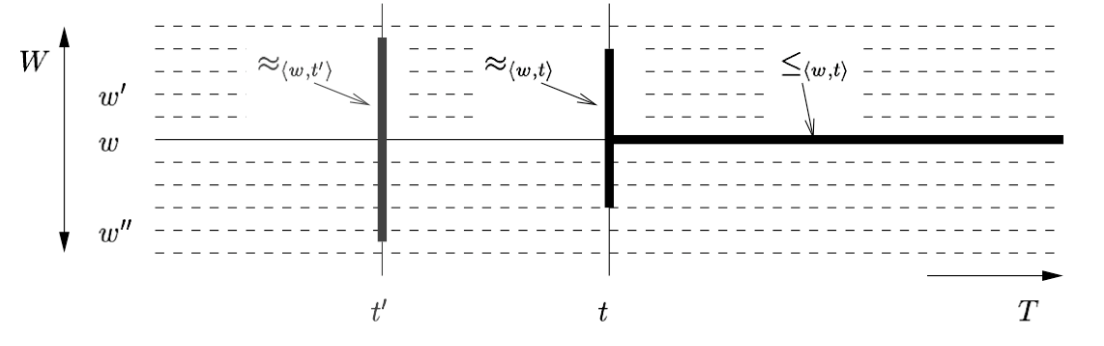
\includegraphics[width=0.8\linewidth]{KCH06-95-WTframe}
	
\end{figure}



At any given index $ i\in\mathcal I $, there is a single past and an infinity of branching futures. Left-linearity (\textit{i.e.}, the tree's trunk) is meant to depict the intuitive fixity (``settledness'') of the past versus the right-branching property, depicting the indeterminacy and openness of the future.
The framework is diagrammed in Figure \ref{BT-dia} below.


\begin{figure}[h]
	\caption[$ \mathfrak T :$ The Branching Times model]{A branching times frame $ \mathfrak T=\langle\mathcal I,\prec\rangle $ following von Prince \citeyearpar[\textit{e.g.},][591]{VonPrince2019}. Time ``flows'' rightwards and vertically aligned indices are taken to be ``copresent''. $\boldsymbol{i*} $ represents the \textit{evaluation index} (present time \& actual world.)}\label{BT-dia}\centering
	\begin{tikzpicture}
		[scale=2,level distance=9mm,
		every node/.style={fill=black,circle,inner sep=1.5pt},
		level 1/.style={sibling distance=10mm},
		level 2/.style={sibling distance=8mm},
		level 3/.style={sibling distance=4mm},
		level 4/.style={sibling distance=2mm},
		edge from parent/.style={draw}]
		\node {} [grow=right]
		child {node {} edge from parent[densely dotted]
			child {node {}
				child {node {}
					child {node {}}
					child {node {}}}
				child {node {}
					child {node {}}
					child {node {}}}}
			child {node {}
				child {node {}
					child {node {}}
					child {node {}}}
				child {node {}
					child {node {}}
					child {node {}}}}}
		child[missing]
		child {node {}
			child {node {} edge from parent[densely dotted]
				child {node {}
					child {node {}}
					child {node {}}}
				child {node {}
					child {node {}}
					child {node {}}}}
			child {node {} edge from parent[densely dotted]
				child {node {}
					child {node {}}
					child {node {}}}
				child {node {}
					child {node {}}
					child {node {}}}}
			child {node [style={fill=red},label=above:$ \boldsymbol{i*} $] {}
				child {node {} edge from parent[densely dashed]
					child {node {}}
					child {node {}}}
				child {node {} edge from parent[densely dashed]
					child {node {}}
					child {node {}}}}};
\end{tikzpicture}\end{figure}

%$ \risingdotseq $
\paragraph{Branches} A branch $b $ which runs through any $ i\in\mathcal I $ is a (maximal) linearly $ \prec $-ordered subset (\textit{sc.} \textit{chain}) of $ \mathcal I $. In this sense, a branch can be taken to correspond to a possible world/a complete possible course of events charting ``an entire possible temporal development of the world'' \citep[148]{Rumberg2019}. If all indices $ i$ are analogous to world-time pairs $\langle w,t\rangle $, then some $ b$ which contains $ i\, (\text{notated }b\ni i)$ is formally a chain of indices, effectively modelling a timeline/set of possible developments of a given world through time --- analogous to a chain over $ \mathcal{W\times T}:\big\langle\langle w,t\rangle,\langle w,t'\rangle,\langle w,t''\rangle,\allowbreak\hdots,\langle w,t_n\rangle\big\rangle$. Note that these frameworks normally appear to assume that indices correspond to the state of a world at a moment of time. I assume that this model can be extended relatively straightforwardly to capture interval semantic notions (\citealp[\textit{e.g.},][]{Landman1991,Dowty1982,Bennett} a.o.). \footnote{This extensibility is also suggested by \citet{Dowty1977} and \citet{Tedeschi1981}, who propose an interval semantic formalism for branching futures. Dowty gives a branching time (re)definition of an interval $ \boldsymbol\imath $ as a connected proper subset ($ \sqsubset $) of a history \citeyearpar[64]{Dowty1977} --- \textit{i.e.}, a ``sub-branch.'' Formally, an interval $ \boldsymbol\imath $ is a subset of $ \mathcal I $ such that: $\exists b\big[\boldsymbol\imath\sqsubset b\wedge\forall i,i',i''\in b[i,i''\in b\wedge i\prec i'\prec i''\to i'\in\boldsymbol\imath]\big] $\label{fn:intervals}}

I will refer to these indices, which constitute the elements of a given branch as \textbf{branchmates}. Given that branches are linearly ordered by $ \prec $, pairs of branchmates are necessarily related by $ \prec $ (and equally by the related linear orders: the weak counterpart $\boldsymbol\preccurlyeq$ and the complements of these two orders $\succ,\succcurlyeq $ respectively.)


\pex Two indices $ i,i' $ are branchmates iff $ i\prec i'\boldsymbol\vee i=i'\boldsymbol\vee i\succ i' $

\xe
And Priorian-type tense operators can be reformulated as asserting relations between pairs of branchmates $ i,i' $( along a given branch $ b $):
\pex
\a$\denote{\textsc{past} \varphi }=\lambda i.\exists i'[i'\prec i\wedge\varphi (i')]$
\a$\denote{\textsc{future} \varphi }=\lambda i.\exists i'[i'\succ i\wedge\varphi (i')]$

\xe


Given that there are, in-principle, infinite logically possible futures for a given index,  $ \mathtt{B}_i $ will be taken to represent the set of all possible branches $ b $ that run through (that is, contain) a given index $ i $ $(\bigcup\limits_{b\scriptstyle\ni i}b)$. This is closely related to the notion of a \textbf{metaphysical modal base}, notated throughout as $ \boldsymbol{\cap{\approx_i}} $, which should be conceived of as comprising the set of branches that represent all the metaphysical/historical alternatives to a given index $ i $ (see (\getref{histaltdef}) for further explication of this important phenomenon.)\footnote{See also \citet{Rumberg2016a} for a discussion of the differences between logical, metaphysical and physical definitions of \textit{possibility} (the alethic modalities.)}

 I'll sometimes also use the notation $ {}^bi $ in quantified expressions as a shorthand restricting the domain of $ \mathcal I $ to a specified branch --- \textit{i.e.}, that subset of $ \mathcal I $ : $ \{i\in\mathcal I\mid i\in b\} $.\footnote{\textit{E.g.}, $ \exists^bi\varphi=\exists i[i\in b\wedge\varphi]$ reads `there exists some index $ i $ along $ b $ s.t. $ \varphi $.'}



\paragraph{The ``co-present''} \citet{Øhrstrøm2020} additionally point out that, for Kripke, these points are ranked with respect to one another --- where each rank (or, diagrammatically, layer) of the tree constitutes an equivalence class of ``co-present'' indices (modally accessible in a $ \mathcal{W\times T }$-model, see \citealp*[95]{Kaufmann2006}).\footnote{Similarly, \citet[194\textit{ff}]{Belnap2001a} distinguish between \textit{moments} (=indices) and \textit{instants}, where the latter are partitions of a tree structure that represent ``[a] horizontal counterpart of histories (=branches).'' ``Rank'' is attributed to Kripke in a 1958 letter to Arthur Prior \citep[published in][373\textit{ff}]{Ploug2012}.} 
That is, indices that are neither successors nor predecessors of one another -- \textit{i.e.}, those are not ordered by $ \prec $ with respect to one another -- can still be temporally compared. In developing a branching-time semantics for conditionals,\footnote{A crucial desideratum of their account is that it formalise Stalnaker's notion of maximal ``similarity'' between the evaluation world and the antecedent proposition, following \citealp{Stalnaker1968,Stalnaker1970}.}$ ^, $\footnote{This formalism, related to the alternativeness relation $ (\approx )$ of \citet[149]{Thomason1984}, has a similar outcome/motivation to the ``Clock'' invoked in \citet{Dowty1977,Thomason1981} and, in later work, the ``instant'' or ``time (value) function'' of \citet[27]{Rumberg2016a}, \citet[195]{Belnap2001a} and \citet[592]{VonPrince2019}, where $ \mathit{\mathsf{time}}$ maps an index to a set of ``clock times'' ordered by $ \prec $ (isomorphic to branches).
	
	Similarly \citet[102]{Landman1991} provides a number of ways of establishing equivalence classes of co-present indices. \textit{E.g.}, in what turns out to be an operationalisation of the Kripke's observation referenced above, ``rank'' can be measured using a function $ d:\mathcal I\to\mathbb N $ that returns the how many ``nodes'' a given index is from $ \mathfrak T $'s defined ``origin'' node (\textit{viz.} $ \bigcirc $ --- the $ \prec $-minimal element of $ \mathcal I $, \textit{cf.} Zorn's lemma). Equivalence classes can then be defined as sets of indices the same number of nodes from the origin, \textit{sc. }$ \approx\underset{\text{def}}{=}\lambda i\lambda i'.d(i)=d(i') $.} 
\cite{Thomason1980} propose an additional ``co-present'' relation $( \boldsymbol\simeq\ \subseteq\mathcal I^2) $ which defines an equivalence class of co-present indices. With the relation $ \simeq $ over $ \mathcal I $, an index can be compared across, \textit{e.g.}, all possible futures. As \citet[101]{Landman1991} points out, in counterfactuals like: \textit{if she hadn't left me a week ago, I wouldn't be so miserable now}, the indexical adverb \textit{now} appears to pick out an index co-present with the time of speech, but crucially on a different ``branch.'' %\footnote{And a ``future choice function'' $ \mathcal F\in\Omega$ which maps individual indices onto a unique history through....}


Armed with this relation then, \citeauthor{Thomason1980} define an (anti)posteriority relation that holds between indices that aren't branchmates:
\pex (Anti)posteriority \citep[311]{Thomason1980}
\a $ i $ is \textbf{posterior} $ (\boldsymbol\succsim )$ to $ j $ iff there is some copresent index of $ j $ (say, $ j' $) that is a successor to $ i $ \hfill
$i \boldsymbol\succsim j\Leftrightarrow\exists j'[j'\simeq j\wedge i\succcurlyeq j'] )$
\a $ i $ is \textbf{antiposterior} to $ j $ iff $ i $ is not posterior to $ j $ or is copresent with $ j $ \\
%$i \precsim j\Leftrightarrow\exists j'[j'\simeq j\wedge i\succcurlyeq j] )$
\xe

\paragraph{Settledness} As suggested above, models of branching time seek to formalise intuitions about asymmetries between past and future predications. We have seen above how the truth of future contingents can be modelled using ``forking paths'' (i.e. branches of linearly ordered subsets of $ \mathcal I $). Conversely, the model is ``left-linear'', depicting `our notion of necessity \textit{given} the past, [where] only one past, the actual one, is possible' \citep[159]{Burgess1978}. That is, for any index there is only one unique sub-branch representing its history/set of predecessors.\label{par:settledness}

\ex \deftagex{ll-def} \textbf{Left linearity }--- \textit{i.e.}, $ \mathfrak T $ is not branching to the past iff --- where $ a,b,b'\in\mathcal I: $\\
$ \forall a.b,b'[(b\prec a\wedge b'\prec a)\to(b\prec b'\vee b=b'\vee b\succ b')] $\trailingcitation{\citep[105]{Landman1991}}\xe

Settledness/historical necessity is normally expressed in terms of \textbf{historical alternatives}. This refers to the notion of equivalence classes of possible worlds $\boldsymbol{(\approx_{t}}\subseteq\mathcal{W\times W})$ : those worlds which have identical `histories' up to and including a reference time $t$. 

The properties of the \textit{historical alternative} relation (in a $ \mathcal{T\times W} $ model) are given in (\nextx) which will permit for a formal definition of settledness as in (\anextx).
	\pex \textbf{Historical alternatives} $\boldsymbol\approx\,\subset\mathcal{T\times W\times W}$\deftagex{histaltdef}
	\a $\forall t[\approx_t\text{ is an equivalence relation}]$\\
	All world-pairs in $\approx_t$ (at an arbitrary time) have identical pasts up to that time.\\Their futures may diverge.\\
	The relation is symmetric, transitive and reflexive (\textit{i.e.}, an equivalence relation).
	\a \textbf{monotonicity}
	
	 $ \forall w,w',t,t'\big[(w\approx_t w'\wedge t'\prec t)\to w\approx_{t'} w'\big]$\\
	Two worlds that are historical alternatives at $t$ are historical alternatives at all preceding times $t'$.\\That is, they can only differ with respect to their futures.\trailingcitation{\citep[146]{Thomason1984}}
	\xe

The monotonicity property (\lastx{b}) captures the intuition that the metaphysical alternatives that are available at given world-time pair change (monotonically) through time: that is, there is a unique possible state of the worlds at all times in the past.  Given that branching-time models are definitionally taken to be left-linear, this additional equivalence relation isn't needed for them: it is a theorem of the system that $ \preccurlyeq $ is monotonic (compare \lastx{b′} below.)

\pex[exno=\getref{histaltdef}]
\a[label=b′] \textbf{monotonicity of $ \boldsymbol\preccurlyeq $}\\$ \forall i,i',i''\big[[i'\preccurlyeq i\wedge i''\preccurlyeq i]\to [i'\preccurlyeq i'' \vee i'' \preccurlyeq i' \vee i=i'']\big] $
\xe


Importantly, the notion of historical alternativeness/necessity is deployed in linguistic semantics to capture a number of natural language phenomena \citep[e.g.,][]{Thomason1984,Condoravdi2002,Kaufmann2002}.

Settledness, a related property, is satisfied if the instantiation of a given predicate is \textbf{identically determined} at all historical alternatives to a given world-time pair $\langle w*,t_0\rangle $ is adapted in (\getref{HistNec}) below).\footnote{That is \textit{settledness} is effectively the union of historical necessity and ``historical impossibility.''}

\pex \textbf{Settledness for\textbf{\textit{\ P}} in $ \boldsymbol{w*}$}\deftagex{HistNec}


$\forall w^{\prime}:w*\approx_{t_0}w^{\prime}:\\\mathit{AT}\big([t_0,\_),w^\prime, \mathit P\big)\leftrightarrow \mathit{AT}\big([t_0,\_),w^{\prime\prime},\mathit{\!P}\big)$%\hspace*{\fill}\citep[82]{Condoravdi2002}\vspace{.25cm}


A property $P$ (\textit{e.g.}, an eventuality) is settled in a reference world $w^\prime$ iff $\mathit P$ holds at a reference time $t_0$ in all of $w^\prime$'s historical alternatives $w^{\prime\prime}$ as calculated at $t_0$.\footnote{The $AT$ relation holds between a time, world and an eventive property iff $\exists e[\mathit P(w)(e)\&\tau(e,w)\subseteq t]$ --- \textit{i.e.} if the event's runtime is a subinterval of $t$ in $w$ (Condoravdi 2002:70). This can accomodate stative and temporal properties with minor adjustments (see \textit{ibid.}). For the sake of perpescuity, I abstract away from (davidsonian) event variables in this section.}
\xe

\noindent Further developing this notion, \citet[82]{Condoravdi2002} gives a definition of ``presumed settledness'' --- a property of predicates \citep[see also][]{Kaufmann2002,Kaufmann2005}. In effect, $ P $ is presumed settled in a given discourse context iff `the instantiation of the property it applies to is presupposed to be historically necessary if true (or equivalently, impossible if false.) This is formalised in (\getref{CondoravdiSett}).\footnote{As a property holding between sentences (rather than properties) and doxastic agents, \citeauthor{Kaufmann2005} similarly defines this condition (`presumption of decidedness') as:
	\exdisplay$\varphi $ is \textbf{presumed decided} by agent $ \alpha $ at $ i $ iff $\underset{\sim\alpha}{\square}(\varphi\to\underset{\approx}{\square}\varphi) $ is true at $ i $.\trailingcitation{\citep[240]{Kaufmann2005}}\\
	That is, iff: in all of $ \alpha$'s doxastic alternatives, if $ \varphi $ holds at $ i $, then it holds at all of $ i $'s historical alternatives.\xe\label{K05-presump}
}


\pex[nopreamble]\deftagex{CondoravdiSett}\a \textbf{The common ground}\deftaglabel{cg}

\textsc{Common beliefs} (somewhat heuristically) are the set of propositions that are taken to be believed by all discourse participants (doxastic agents) $ \alpha $ in the discourse context $ (c) $.

\textit{\textsc{cb}}$ _c(\varphi) \underset{\texttt{def}}{=} \varphi\in \underset{\alpha\in c}{\bigcap} \textsc{dox}_\alpha (w*) $

\textsc{The common ground}  $ \mathit{cg_c} $, then, is the transitive closure of the common belief relation (that is, an ancestral relation, \citealp[compare][]{Stalnaker2002,Kaufmann2010,Fagin}.)

$ \mathit{cg_c}(\varphi)=\varphi\in\bigcup\limits_{i=1}^\infty\textit{\textsc{cb}}_c^i\text{, where }\textsc{\textit{cb}}^{i+1}_c\varphi=\textsc{\textit{cb}}_c\textsc{\textit{cb}}^{i}_c\varphi $ 

That is, a proposition $ \varphi $ is in the common ground iff it is a common belief of all participants that it is a common belief of all participants \textit{etc.} that $ \varphi $.


\a \textbf{The presumption of settledness for $\boldsymbol P$}\deftaglabel{pres}


$\forall w^\prime:w^\prime\in\cap cg,\forall w^{\prime\prime}:w^\prime\approx_{t_0}w^{\prime\prime}:\\\mathit{AT}\big([t*,\_),w^\prime, P\big)\leftrightarrow \mathit{AT}\big([t*,\_),w^{\prime\prime},\!P\big)$\hspace*{\fill}\citep[82]{Condoravdi2002}\vspace{.25cm}

%todo edit
A property $P$ (\textit{e.g.} an eventuality) is presumed settled in a common ground $cg$ iff $P$ is settled at all historical alternatives $ w'' $ to all worlds $ w' $ compatible with $ cg $.

Here, a common ground is taken to be to be equivalent to a context set \citep[$ \cap\textit{cg} $, \textit{cf.}][321\textit{ff}]{Stalnaker1978} --- \textit{sc. }the set of worlds that the speaker takes to be epistemically accessible for participants in the discourse context/the set of worlds where all propositions known by the discourse participants are true (compare also \citeauthor{Kaufmann2005}'s definition of settledness (``decidedness'') in fn.~\ref{K05-presump}).
\xe

Once again, and drawing on the relations described above, this relation between context set and property (\getref{HistNec}) can be recast in a branching-time model as in (\getref{HistNec}′); again $ i*\in\mathcal I $ represents the evaluation/reference index (analogous to $ \langle w_0,t_0\rangle $ above).

\pex[exno=\getref{HistNec}′]\textbf{Settledness-at-$ \boldsymbol{i*} $ for $ \boldsymbol{\mathit P} $} (branching times)\deftagex{SettBT}\deftagpage{SettBTp}


%$ \forall i'\big[i'\preccurlyeq i\to\exists i''[i''\succ i'\wedge\mathit{AT}(P,i'')]\big] $A property $ P $ is settled at a reference index $ i $ iff, at all predecessor indices $ i' $, all indices $ i'' $ that succeed $ i' $, $ P $ is instantiated.

%$\forall i^\prime:i^\prime\preccurlyeq i*,\exists i''\succcurlyeq i':\\
%\mathit{AT}\big(i', P\big)\leftrightarrow \mathit{AT}\big(i'',\!P\big)$

%%%%%defense version
%\nobreak$\forall b\bigg[b\in\texttt{B}_{i*}\to\exists i'\Big[i'\in b\wedge\forall j\big[i'\simeq j\wedge[\mathit{AT}\big(i', \mathit{P}\big)\leftrightarrow \mathit{AT}\big(j,\mathit{P}\big)]\big]\Big]\bigg]$

\nobreak$\forall b_1,b_2\in\cap{\approx_{i*}}:\exists^{b_1}i'\exists^{b_2}i''\big[i'\simeq i''\wedge [P(i')\leftrightarrow P(i'')]\big]$

\nobreak A property $ P $ is settled at an evaluation index $ i* $ \textbf{iff} for any arbitrary pair of branches $ b_1,b_2 $ that represent metaphysical alternatives to $ i* $, there is a pair of copresent indices $ i',i'' $ such that \textit{P} holds at $ i' $ iff it also holds at $ i'' $ (that is, \textit{P} is identically determined at co-present alternative indices.)

%%DEFENSE VERSION%all branches running through evaluation time $ i* $ contain a co-present index $ j\in\cup\simeq i' $ such that $ P $ is instantiated at $ i' $ iff it's also instantiated at $ j $. (\textit{I.e.}, $ P $ is settled at $i* $ iff it's instantated at all or none of the indices that are copresent with $ i' $ (a branchmate of $ i* $.))
\xe

\noindent Similarly, in a branching time framework, we would stipulate that $ P $ is \textbf{presumed settled} iff, for any possible branch $ b $ that is compatible with a given common ground, $ P $ is identically determined at $ b $ and all of $ b $'s historic alternatives.



\paragraph{A modal trichotomy}\label{vP-trich} As a consequence of this,  \citeauthor{VonPrince2017a} (\citeyear{VonPrince2017a,VonPrince2019}; \citealp{VonPrincea} forthcoming) establishes a neat formal trichotomy between the \textsc{actual, potential} and \textsc{counterfactual} domains by appealing to this framework \citetext{\citealp[see also][41]{Rumberg2016a}, \citeyear{Rumberg2019}}. This is modelled as having $ \boldsymbol{\prec} $ induce a partition of $ \mathcal I $: that is, all $ i\in\mathcal I $ can be sorted into (exactly) one of these three sets. This partition is reproduced in (\getref{trichot}).

\pex Given a contextually defined \textsc{actual present} $( i*\doteqdot\langle w*,t*\rangle )$, $ \mathcal I $ can be partitioned into three subdomains:
\a The \textsc{actual} (past/present) = $\boldsymbol{ \{i\mid i\preccurlyeq i*\} }$

The utterance index $ i* $ and its predecessors are the realm of the \textsc{actual}.
Compare this notion to the equivalent one of \textit{historical alternatives to $ w $ at $ t $}. These indices will be shown to be associated with the (notional semantic category of) \textsc{realis}.
\a The \textsc{potential} = $ \boldsymbol{\{i\mid i\succ i*\} }$

Successors to the index of utterance $ i* $ are the realm of the \textsc{potential}: the full set of metaphysically possible futures to $ i* $.

\a The \textsc{counterfactual} = $\boldsymbol{ \{i\mid i \textbf{ is unordered by $ \boldsymbol\prec $ w/r/t } i* \}}$

Those $ i\in\mathcal I $ which neither precede nor succeed the utterance index $ i* $: i.e., indices that are not (possible) branchmates of $ i* $.

\deftagex{trichot}\deftagpage{vP-bt0}
\xe

 Each cell of this partition is represented in Figure \ref{BT-dia} above: solid lines join those indices that are \textsc{$ i* $-actual}, whereas dashed and dotted lines represent \textsc{$ i* $-potential} and \textsc{-counterfactual} branches respectively. This trichotomy is shown to have significant linguistic import (which will be explored throughout the dissertation.)

\subsection[Modal auxiliaries as quantifiers]{Modal auxiliaries as quantifiers: \citealt{Kratzer1977} \textit{et seq.}}\label{sec:kratzer}
 Building on the tense logics introduced above, following (Kratzer \citeyear{Kratzer1977,Kratzer1981,Kratzer1991} a.o.), modal expressions are taken to denote \textbf{quantifiers over possible worlds}. Crucially, like other natural language quantifiers, modal auxiliaries are taken to contain (implicit) restrictions over their quantificational domain. For Kratzer the distinction between so-called \textit{epistemic} and \textit{deontic} readings of modal auxiliaries is a function of this restriction. This distinction is shown in the sentence pair in (\getref{K77-mod}) below.

\pex Two readings of English modal auxiliary \textit{must} from \citet[338]{Kratzer1977}\deftagex{K77-mod}
\a\textit{All Māori children \textbf{must} learn the names of their ancestors}\deftaglabel{de}
\a\textit{The ancestors of the Māori \textbf{must} have arrived from Tahiti}\deftaglabel{ep}
\xe

In effect, the different readings (``flavours'') of \textit{must} in (\getfullref{K77-mod.de}-\getref{K77-mod.ep}) arise as a consequence of different \textbf{restrictions} that are made over the set of possible worlds. In effect, the deontic reading (\getfullref{K77-mod.de}) makes a claim about only (and all) those worlds/possible states-of-affairs in which Māori children adhere to some set of societally-given rules, laws and expectations. Conversely (\getfullref{K77-mod.ep}) makes a claim about only (and all) those possible worlds that are compatible with everything that the speaker knows. These subsets of $ \mathcal W$ are referred to as \textbf{conversational backgrounds} (\textit{sc.} an \textit{epistemic} vs. \textit{deontic} conversational background). By assuming that conversational backgrounds are supplied by broader lingusitic context, a major advantage of the Kratzerian program is that modal auxiliaries like \textit{must} and \textit{can} can be taken to be semantically unambiguous. The accessibility relations against which modal propositions were verified in earlier modal logics (sc. modals as unary operators) are reconceptualised as contextually-retrieved functions from worlds to (sets of) propositions \citep*[see][]{Kaufmann2006}. 


 A sentence of the form \textit{must} $ \varphi $ asserts that $ \varphi $ is true in all relevant worlds (universally quantifying over a subset of $ \mathcal W $, returned by a \textbf{modal base} (\textit{i.e.}, a conversational background $ f $) whereas one of the form \textit{can $ \varphi $} makes a weaker claim, namely that the truth of $ \varphi $ is \textit{compatible} with those worlds. That is, \textit{must} is a universal quantifier and \textit{can} is an existential quantifier over possible worlds (\nextx). %Consequently, on formal accounts, modal operators are analysed as 

\pex\textbf{ The semantics of necessity/possibility modal auxiliaries }\trailingcitation{\citep[adapting from][346]{Kratzer1977}}\deftagex{K-modals}
\a $ \denote{\textit{must~}}=\lambda f\lambda p\lambda w.\forall w'[w'\in\cap f(w)\to w'\in p] $

\textit{must $ p $} is true given a modal base $ f(w) $ if $ p $ follows from $ f(w) $


\a $ \denote{\textit{~can~}}=\lambda f\lambda p\lambda w.\exists w'[w'\in\cap f(w)\wedge w'\in p] $

\textit{can $ p $} is true given a modal base $ f(w) $ if $ p $ is compatible with $ f(w) $

\xe

A second type of conversational background, the \textbf{ordering source}, is formally similar to the modal bases invoked above insofar as it comprises a set of propositions $ o(w) $. This set can induce an \textit{ordering} over the worlds in the modal base in terms of how well each world conforms with $ o(w) $. Appealing to multiple interacting conversational backgrounds has allowed for successful modelling of linguistic expressions that denote/appeal to graded possibilities and probability and subtle differences in modal ``flavours.'' That more than one conversational background is required is well illustrated in (\nextx) (adapted from \citealp*{Kaufmann2006}).

\pex \textit{Randi must pay a fine for drink-driving}\\ $ \boldsymbol{\not\Rightarrow }$ `In all those worlds where the rules are best followed, Randi must drink-drive.'\label{ex:randi}\xe

\noindent(\lastx) shows that a deontic conversational background can't serve as the modal base for \textit{must} (as this would require that all law-abiding worlds be characterised by Randi's drink-driving.) Instead, we appeal to a ``circumstantial'' modal base $ m(w) $: that is, we consider worlds where relevant circumstances (including Randi's drink-driving) obtain, and universally quantify into a subset of those, namely the ones that best conform to whichever set of rules/laws govern drink-driving (\textit{sc.} those propositions in the deontic ordering source $ o(w) $.) Generally this is operationalised by appealing to a function $ \underset{o(w)}{\textsc{best}}$ which takes a set of worlds and returns the ``best'' worlds as determined by an ordering source $ o $ (\textit{i.e.}, those worlds in $ m $ best conforming to the ideal contained in $ o $ as in (\nextx) adapted from \citealp[61]{VonFintel2011}.)\footnote{This same function is sometimes also given as \textbf{\textit{max}} (\citealp[\textit{e.g.},][]{Hacquard2006,VonFintel2008,VonFintel2011}, a.o.) or \textbf{\textit{O(pt)}} \citep[247]{Schwager2006}.} Armed with this function, we can implement an ordering semantics for modal auxiliaries, as in (\getref{must.mo}).

\ex \textbf{The best worlds in a modal base $ m $ according to an ordering} $\boldsymbol{\underset{o(w)}{\prec}}$

$ \underset{o(w)}{\textsc{best}}\big((\cap m(w)\big)=\{w\in\cap m(w)\mid \neg\exists w'[w'\underset{o(w)}{\prec}w]\}$\label{ord-source}\xe
\pex \textbf{\textit{must} relativised to two conversational backgrounds} (modal base $ m $ and ordering source $ o $)\deftagex{must.mo}

$\denote[o,m]{\textit{must}}=\lambda p\lambda w.\forall w'[w'\in\underset{o(w)}{\textsc{best}}(\cap m(w))\to w'\in p] $

\textit{must $ p $} is true in $ w $, given conversational backgrounds $ \langle{m,o}\rangle $ if $ p $ is in true in all the worlds that are best conforming to $ o(w) $ in $ \cap m(w) $
\xe





The formal implementation of orderings and comparisons of sets of worlds (or branches) will be further discussed in the main part of this dissertation.

\paragraph{Quantifying over $ \mathfrak{T} $}

Once again, we can recast the contribution of modal expressions within a branching-times type ontology (suggested in \citealp[594, note 9]{VonPrince2019}). In such a system, modals will be taken to quantify over branches $ (\mathcal{B\subseteq\wp(I)})$ --- again, maximal chains within $ \mathcal I $ or sets of indices that are linearly ordered by $ \prec $. Given that each unique branch represents a possible course of events, modal operators can be taken to quantify over $ \mathcal B $, much as they do over $ \mathcal W $ in possible world semantics.

This involves recasting conversational backgrounds --- sets of propositions --- as functions from indices to sets of possible branches of $ \mathcal I $. A deontic conversational background $ \textsc{deont}(i) $, for example, is a set of propositions which represent the body of laws at a given index $ i $. As in possible worlds analyses, these conversational backgrounds restrict the domain of quantification to some contextually relevant subset of  $ \texttt{B}_i $ --- i.e. a subset of those branches that run through $ i $.

Below, I propose a basic Branching-theoretic modification to the  lexical entries for the English modal auxiliaries that was provided in (\getref{K-modals}).\footnote{Ordering sources can be added back in straightforwardly (\textit{i.e.}, again as sets of propositions which induce an order over a modal base.) They are not given in these entries for the sake of exposition.}

\pex[exno=\getref{K-modals}′⁣] \textbf{A proposed modification to semantics for modal auxiliaries (\getref{K-modals}) for $ \mathfrak T $-frames.}
\a$ \denote[m]{\textit{must}}=\lambda p\lambda i.\forall b\ni i[b\in\cap m(i)\to \exists i':i'\in b\wedge p(i')] $\\
%\textit{must $ p $} is true given a modal base $ f(i) $ is $ p $ follows from $ f(i) $...?
\textit{must} $ p $ is true if, along all the branches through $ i $ that are selected by the modal base $ m(i) $, there is a branchmate $ i' $ such that $ p $ holds at $ i' $.

\a$ \denote[m]{\textit{can}}=\lambda p\lambda i.\exists b\ni i[b\in\cap m(i)\wedge \exists i':i'\in b\wedge p(i')] $\\
%\textit{must $ p $} is true given a modal base $ f(i) $ is $ p $ follows from $ f(i) $...?
\textit{ can } $ p $ is true if, there is some branch running through $ i $, which is selected by the modal base $ m(i) $ and along that branch there is an index $ i' $ such that $ p $ holds at $ i' $.


\xe


\fancybreak 
As mentioned above, the vast majority of work in the formal semantic program has taken European languages as its object of study. If model-theoretic approaches to semantics are to provide a complete theory of natural language phenomena, it is incumbent upon the field to demonstrate the applicability of these tools and principles to all possible human languages. This enterprise includes modelling and precisely describing the diversity of temporal and modal systems cross-linguistically.

For example, recent work on cross-linguistic semantics has shown how the semantics for English modals -- where quantificational force is lexically encoded and conversational backgrounds are provided by context -- does not provide the correct semantics for other languages' modal systems. \citet{Rullmann2008}, for example show that, in St̓át̓imcets (\gls{lil} Salish: British Columbia), deontic and epistemic modal clitics are separately lexified whereas quantificational force is contextually determined (\textit{viz.} \textit{ka}~`\textsc{irr}', \textit{kˀa}~`\textsc{epist}' and \textit{kelh}~\textsc{fut}') \citep[see also][]{Peterson2010,Matthewson2010}. They model this with a choice function $ f_{\mathfrak c}$, pragmatically provided that restricts the size of the set (\textit{sc.} modal base) which is being universally quantified over (\nextx).\footnote{\citet{Deal2011} shows that a similar phenomenon in Niimiipuutímt [\gls{nez}] suggests an analysis of a variable-force modal as an existential quantifier. She claims that, because there is no ``stronger'' circumstantial modal competitor to \textit{-o'qa} `\gls{mod}', the variable force phenomenon (her ``quantificationally variable modal[ity]'') is a result of a single lexical item performing all modal functions.}

\pex Semantics for \textit{kˀa} `\gls{epist}' (St̓át̓imcets epistemic variable-force modal, from \citealp[340]{Rullmann2008})

\denote[c,w]{\textit{kˀa}} presupposes an epistemic modal base $ m $ \&\\
$ \denote[c,w]{\textit{kˀa}}=\lambda f_{\mathfrak c}\lambda p.\forall w'[w'\in f_{\mathfrak c}(m(w))\to p(w')]$
\xe

Building on other insight on usage of possibility modals \citep[notably][]{Klinedinst2007}, for \citet{Rullmann2008} the ``appearance'' of force variability in St̓át̓imcets modals is a result of the relative size of the subset of the modal base picked out by $ f_{\mathfrak c} $ (that is, quantifying over a smaller subset makes a commensurately weaker modal claim.) Numerous authors have since pointed out that this appeal to $ f_{\mathfrak c} $ seems to be actually equivalent to deploying an ordering source as described above (and similarly to \citeauthor{VonFintel2008}'s 2008 treatment of \textit{ought} ``strong necessity'' --- \citealp[see][]{Portner2009,Matthewson2010,Peterson2008}.)
 A similar phenomenon (\textit{viz.} force variability) is exhibited in Western Dhuwal(a); see Part \textbf{\ref{yolŋu}}, which will deploy components of this analysis. As we will see through this dissertation, additional elaborations and assumptions will permit us to capture facts about the grammars of these Australian languages.

\section{A note on the ``amphichronic program''}\label{amph}

Due to Kiparsky (\citeyear{Kiparsky2006} \textit{et seq.}), \textit{amphichronic} linguistics is an approach to linguistic theory that assumes that synchronic and diachronic levels of explanation ``feed each other'' \citep[see also][]{Bermudez-Otero2013}. This research program is motivated by the necessity to dissociate \textit{typological generalisations} from \textit{language universals}. Are the phenomena that we see (or don't see) expressed in natural language a function of universal design features and constraints on the human language faculty? Or are they derivable ``by-products'' from tendencies of language change? \citep[see also][]{Anderson2008,Anderson2016a}.%\marginnote{further elaboration; explanation of ``diachronic level of explanation''}

In the semantic domain, for Kiparsky, ``[grammaticalisation] reveals the langauge faculty at work. Formal renewal engenders new categories that conform to cross-linguistic generalisations regardless of their source'' \citep[73]{Kiparsky2015}. Over past decades, research on meaning change has led to the discovery of regular grammaticalisation ``clines/pathways/trajectories'': that is, a given lexical expression with meaning $ \alpha $ comes to denote $ \beta $, then $ \gamma $ \textit{etc.} as an independent development across languages separated in space and time \citep[see][]{Deo2015,Eckardt2011}. From the identification of these robust cross-linguistic tendencies emerges the question of what is driving this change and \textbf{\textit{why}}.

As an example, \citet{Bybee1994} present a hypothesis that grammaticalisation pathways ought to be derivable from the meanings of the lexical items involved in them; frequently these changes involve the ``generalisation'' of a given item. As \citet[7]{Leow2020} points out, this idea has been taken seriously by diachronic semanticists, where \textit{generalisation} has been modelled as the expansion in the functional domain of a given expression \citep[\textit{e.g.},][]{Deo2015a,Condoravdi2014}.\footnote{Also James Leow's recent \citeyearpar{Leow2020} dissertation which conceives of variation and change in (semi)modal expressions in Cuban Spanish (viz. \textit{\textsc{iba} a, tener que}) as reflexes of grammaticalisation.

A concise history of formal diachronic semantics as a research program is provided in \citet{Yanovich2020}.} 
 Hypotheses involving the apparent \textit{unidirectionality} of grammaticalisation trajectories are taken to be a reflex of a cross-linguistic tendency for meanings to ``generalise.''

 In this dissertation, I apply a methodology where the precise synchronic meaning of particular linguistic expressions is analysed while simultaneously attending to changes in the interpretive conventions associated with these expressions.
 
 It is a goal of the current research, then, to contribute insights into the ætiology of these changes and to consider what light, if any, they may shed on the universal ``structure'' of the semantic domains that are investigated here.

\section{The linguistic ecology of Arnhem Land}\label{sec:ecol}

%Initial human inhabitation of the Australian landmass is generally estimated at roughly 50,000 years ago (50Kya).
The past few decades have seen mounting interest in the deployment of historical\slash{}comparative linguistic methods for uncovering linguistic and anthropological prehistory of the continent \citetext{\citealp[see][]{McConvell2011} for an overview.} Some three hundred Australian languages have been reconstructed to a single family, Pama-Nyungan, spoken across mainland Australia (approx. 90\% of its area) except for some regions in the north of the continent \citep{Dixon1980,Bowern2021}. The most recent common ancestor of these languages (\textit{sc. proto-Pama-Nyungan}) is estimated to have been spoken roughly five to seven thousand years before present (5--7Kya, during the mid-Holocene/Northgrippian age: a comparable timedepth to Indo-European), originating in the ``Gulf Plains'' bioregion around the Gulf of Carpentaria \citetext{\citealp{Bouckaert2018}, supporting earlier work, incl. \citealp{Hale1964} a.o.}. Many of these languages remain underdescribed (extinct, or recorded in ``salvage''-oriented documentatary work.) As a consequence, they are by and large poorly integrated into (model-)theoretic treatments of cross-linguistic semantics (as suggested in \S~\ref{sec:overview} above, see also \citealp{Nordlinger2021} for an overview of the impact of theoretical treatments of Australian language data.)

%\begin{figure}[h]\caption[Australian language maps]{Map of Australian linguistic areas, including detail of Northern Australia and Arnhem Land}\label{maps}
%	\begin{subfigure}[t]{\textwidth}
\begin{figure}
		\caption[\textsc{map.} Australia \& the top end]{Australian language families: Pama-Nyungan is shaded yellow, with detail of diverse Northern Australia \citep[adapted from][]{Dixon2002a}}\label{pn}\centering
		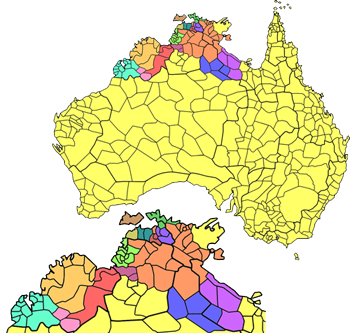
\includegraphics[width=.6\linewidth]{ALs.png}
	\end{figure}
%\clearpage
%\begin{subfigure}[t]{\textwidth}
\begin{figure}
	\caption[\textsc{map.} Languages of Arnhem Land]{Languages of Arnhem Land. \textit{Yolŋu}-speaking area is shaded. Primary data in this dissertation was elicited in Ramingining \& Ngukurr (highlighted). Map adapted from \citet[2]{Wilkinson1991}.}\label{arn}\centering
		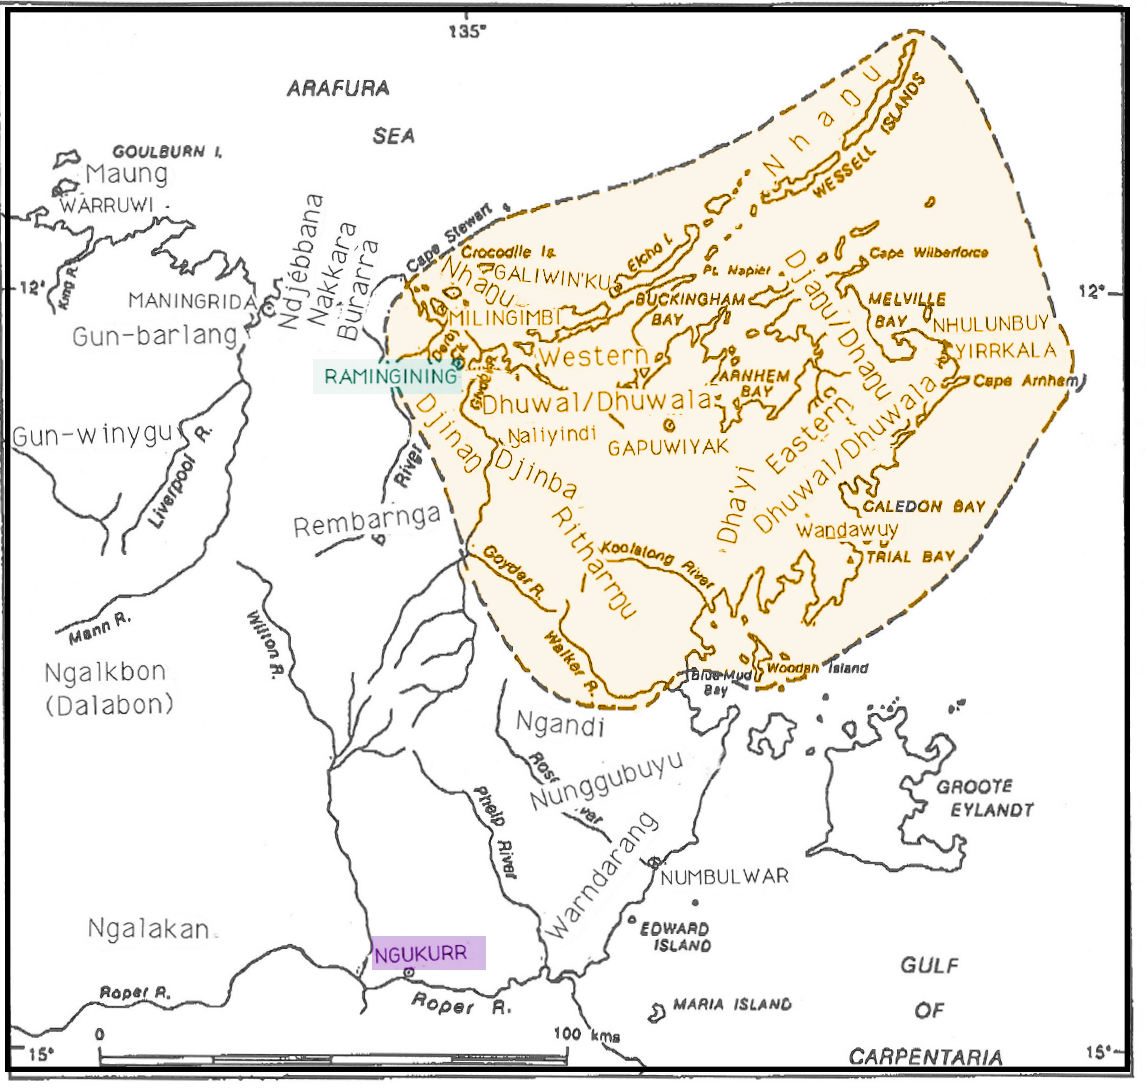
\includegraphics[width=.85\linewidth]{arnhem-mw2.png}
%\end{subfigure}
\end{figure}

\paragraph*{Multilingualism}

Arnhem land --- detail provided in figure \ref{arn} --- is a linguistically diverse region of Australia's ``Top End.'' Relatively isolated (several hundred kilometers east of Darwin), the population is roughly 85\% indigenous, home to a number of ethnolinguistic groups. Owing to the relative isolation of northern Australian communities, 12 of the 20 aboriginal languages judged as ``strong'' are spoken in the Northern Territory \citep[3]{Schmidt1990}. Language families spoken in Arnhem Land include Yolŋu (Pama-Nyungan) in the northeast, surrounded by a number of non-Pama-Nyungan isolates as well as the Iwaidjan, Maningrida/Burarran, Gunwinyguan, Rembarngic, Marran and SE Arnhem families; the constituency of these groupings and the relations between them are still uncertain \citetext{see \textit{e.g.}, \citealp{Green2003} for the proto-Arnhem proposal.} Assessing these relations is complicated by the especially high degree of language contact and endemic ``personal multilingualism'' that characterise Arnhem Land speech communities, patterns reinforced by universal moiety/clan exogamy \citetext{\citealp{McConvell2011,Evans2001}, see also \citealp[Ch. 1]{Williams1986,Wilkinson1991} for a discussion of clan exogamy in Yolŋu society}. Children are raised in multilingual settings and continue acquiring new languages throughout their life. 

\paragraph*{Endangerment \& displacement}

As suggested above, the effects of European invasion of the Australian continent in the eighteenth century were catastrophic for Aboriginal Australia; one consequence of this being the fragmentation of traditional language ecologies. According to \citet[1]{Schmidt1990}, two-thirds of Australian languages spoken at the time of contact (which she, perhaps conservatively, numbers as 250) are no longer spoken. She estimates that only one in every ten Aboriginal people speaks their indigenous language. Westward frontier expansion had the effect of bringing Aboriginal pidgin varieties into Arnhem Land, which subsequently developed into a creole language. With varieties estimated to be spoken by more than 30,000 people across Northern Australia, Australian Kriol is understood to have first emerged as a community language in the Roper Gulf region (SE Arnhem), close to the contemporary community of Ngukurr \citetext{\textit{e.g.}, \citealp{Harris1986a}, see also \citealp{Phillips2011} for an overview.} Kriol continues to be the first language of the vast majority of Ngukurr's indigenous population; with a couple of exceptions, most of the traditional Australian languages of the area are now critically endangered (see also chapter \ref{bambai.desc}.)


Additional background information on the sociolinguistic context of the language varieties under investigation is provided in each chapter.


\section{Data \& glossing conventions}

Each subpart of this dissertation makes use of (novel and published) data from different sources. Example sentences are glossed following (modified) Leipzig conventions (all adopted abbreviations listed on \textit{pg.} \pageref{glossing}).

 I adopt standard orthographic conventions for Yolŋu Matha (including the standardisation of other sources written in IPA or other Australian language transcription conventions to Yolŋu spelling conventions.) These writing systems are derived from English orthography; digraphs and diacritics which may be unfamiliar or otherwise ambiguous to the reader and their IPA (International Phonetic Alphabet) correspondences are tabulated below \citetext{Table \ref{tab:orthogr}. See also, \textit{e.g.}, \citealt[549]{Dixon2002a} for an overview of ``canonical'' phoneme inventories in Australian Language and \citealp{Wilkinson1991} for the Yolŋu orthography (\textit{pp.} 41--4), due to Beulah Lowe and a general discussion of the Djambarrpuyŋu phoneme inventory.}

\begin{table}[h]
\caption[Orthographic conventions]{Correspondences between \textbf{\texttt{[IPA]}}, \textcolor{DarkOrchid}{\textbf{\textit{Australianist}}} and \textcolor{BrickRed}{\textbf{\textit{Yol\kern -0.2pt ŋu}}} orthographic conventions adopted in the dissertation}	\label{tab:orthogr}\centering
	\begin{tabular}{>{[~}l<{~]}>{\it\color{DarkOrchid}}c>{\it\color{BrickRed}}c@{\hskip 1.5em}>{[~}l<{~]}>{\it\color{DarkOrchid}}c>{\it\color{BrickRed}}c@{\hskip 1.5em}>{[~}l<{~]}>{\it\color{DarkOrchid}}c>{\it\color{BrickRed}}c}

\multicolumn{3}{c}{\textcolor{Gray}{\textsc{obstruents}}} & \multicolumn{3}{c}{\textcolor{Gray}{\textsc{sonorants}}} & \multicolumn{3}{c}{\textcolor{Gray}{\textsc{vowels}}}\\
		 b & \multicolumn{2}{c}{\textit{b}}& m &\multicolumn{2}{c}{\textit{m}}&	ɐ&a&a\\
	 p & \multicolumn{2}{c}{\textit{p}}&\multicolumn{3}{c}{}&	ɐː&aa&ä\\
	d̪&\multicolumn{2}{c}{\textit{dh}}&n̪&\multicolumn{2}{c}{\textit{nh}}&ɪ&i&i \\	
	t̪&\multicolumn{2}{c}{\textit{th}}&\multicolumn{3}{c}{}&	ɪː&i&e\\
		d&\multicolumn{2}{c}{\textit{d}}& n &\multicolumn{2}{c}{\textit{n}}&	ʊ&u&u\\	
	t&\multicolumn{2}{c}{\textit{t}}&l&\multicolumn{2}{c}{\textit{l}}&	ʊː&uu&o\\	
 ɖ&rd&ḏ& 	ɳ&rn&ṉ&\multicolumn{3}{c}{\textcolor{Gray}{\textsc{rhotics/glides}}} \\
	ʈ&rt&ṯ&ɭ&rl&ḻ&	ɻ&\multicolumn{2}{c}{r}\\
ɟ&j/dy&dj&	ɲ&ny & ny&ɾ&\multicolumn{2}{c}{\textit{rr}}\\
	c&ch/ty&tj&\multicolumn{3}{c}{}&j&\multicolumn{2}{c}{\textit{y}}\\
	g&\multicolumn{2}{c}{\textit{g}}&ŋ&ng&ŋ	& w&\multicolumn{2}{c}{\textit{w}}\\
		k&\multicolumn{2}{c}{\textit{k}}\\
	ʔ&---&ˀ\\
	\end{tabular}
\end{table}

% Please add the following required packages to your document preamble:
% \usepackage{multirow}
% \usepackage[table,xcdraw]{xcolor}
% If you use beamer only pass "xcolor=table" option, i.e. \documentclass[xcolor=table]{beamer}
	%\begin{table}[]
	%	\begin{tabular}{llllllll}
	%		\cellcolor[HTML]{FFFFFF}{\color[HTML]{333333} } &                                                                                 &                                                                                   & \multicolumn{2}{l}{apico}                                                                                                                                                                                                                                                                                                                                                                      &                                                                                                                                                                                                   &                                                                                                                                                                                                &                                                                                                                                                                                              \\
	%		\cellcolor[HTML]{FFFFFF}                        & \multirow{-2}{*}{labial}                                                        & \multirow{-2}{*}{dental (lamino)}                                                 & alveolar                                                                                                                                                                                       & retroflex                                                                                                                                                                                     & \multirow{-2}{*}{palatal (lamino)}                                                                                                                                                                & \multirow{-2}{*}{velar}                                                                                                                                                                        & \multirow{-2}{*}{glottal}                                                                                                                                                                    \\
	%		lenis                                           & \begin{tabular}[c]{@{}l@{}}{[}p{]}\\ \textbackslash{}textit\{⟨p⟩\}\end{tabular} & \begin{tabular}[c]{@{}l@{}}{[}t̪{]}\\ \textbackslash{}textit\{⟨th⟩\}\end{tabular} & \begin{tabular}[c]{@{}l@{}}{[}t{]}\\ \textbackslash{}textit\{⟨t⟩\}\end{tabular}                                                                                                                & \begin{tabular}[c]{@{}l@{}}{[}ʈ{]}\\ \textbackslash{}textcolor\{violet\}\{\textbackslash{}textit\{⟨rt⟩\}\}\\ \textbackslash{}textcolor\{ochre\}\{\textbackslash{}textit\{⟨ṯ⟩\}\}\end{tabular} & \begin{tabular}[c]{@{}l@{}}{[}c{]}\\ \textbackslash{}textcolor\{violet\}\{\textbackslash{}textit\{⟨ch/ty⟩\}\}\\ \textbackslash{}textcolor\{ochre\}\{\textbackslash{}textit\{⟨tj⟩\}\}\end{tabular} & \begin{tabular}[c]{@{}l@{}}{[}k{]}\\ \textbackslash{}textit\{⟨k⟩\}\end{tabular}                                                                                                                & \begin{tabular}[c]{@{}l@{}}{[}ʔ{]}\\ \textbackslash{}textcolor\{violet\}\{\textbackslash{}textit\{---\}\}\\ \textbackslash{}textcolor\{ochre\}\{\textbackslash{}textit\{⟨ˀ⟩\}\}\end{tabular} \\
	%		fortis                                          & \begin{tabular}[c]{@{}l@{}}{[}b{]}\\ \textbackslash{}textit\{⟨b⟩\}\end{tabular} & \begin{tabular}[c]{@{}l@{}}{[}d̪{]}\\ \textbackslash{}textit\{⟨dh⟩\}\end{tabular} & \begin{tabular}[c]{@{}l@{}}{[}d{]}\\ \textbackslash{}textit\{⟨d⟩\}\end{tabular}                                                                                                                & \begin{tabular}[c]{@{}l@{}}{[}ɖ{]}\\ \textbackslash{}textcolor\{violet\}\{\textbackslash{}textit\{⟨rd⟩\}\}\\ \textbackslash{}textcolor\{ochre\}\{\textbackslash{}textit\{⟨ḏ⟩\}\}\end{tabular} & \begin{tabular}[c]{@{}l@{}}{[}ɟ{]}\\ \textbackslash{}textcolor\{violet\}\{\textbackslash{}textit\{⟨j/dy⟩\}\}\\ \textbackslash{}textcolor\{ochre\}\{\textbackslash{}textit\{⟨dj⟩\}\}\end{tabular}  & \begin{tabular}[c]{@{}l@{}}{[}g{]}\\ \textbackslash{}textit\{⟨g⟩\}\end{tabular}                                                                                                                &                                                                                                                                                                                              \\
	%		nasal                                           & \begin{tabular}[c]{@{}l@{}}{[}m{]}\\ \textbackslash{}textit\{⟨m⟩\}\end{tabular} & \begin{tabular}[c]{@{}l@{}}{[}n̪{]}\\ \textbackslash{}textit\{⟨nh⟩\}\end{tabular} & \begin{tabular}[c]{@{}l@{}}{[}n{]}\\ \textbackslash{}textit\{⟨n⟩\}\end{tabular}                                                                                                                & \begin{tabular}[c]{@{}l@{}}{[}ɳ{]}\\ \textbackslash{}textcolor\{violet\}\{\textbackslash{}textit\{⟨rn⟩\}\}\\ \textbackslash{}textcolor\{ochre\}\{\textbackslash{}textit\{⟨ṉ⟩\}\}\end{tabular} & \begin{tabular}[c]{@{}l@{}}{[}ɲ{]}\\ \textbackslash{}textit\{⟨ny⟩\}\end{tabular}                                                                                                                  & \begin{tabular}[c]{@{}l@{}}{[}ŋ{]}\\ \textbackslash{}textcolor\{violet\}\{\textbackslash{}textit\{⟨ng⟩\}\}\\ \textbackslash{}textcolor\{ochre\}\{\textbackslash{}textit\{⟨ŋ⟩\}\}\end{tabular}  &                                                                                                                                                                                              \\
	%		lateral                                         &                                                                                 &                                                                                   & \begin{tabular}[c]{@{}l@{}}{[}l{]}\\ \textbackslash{}textit\{⟨l⟩\}\end{tabular}                                                                                                                & \begin{tabular}[c]{@{}l@{}}{[}ɭ{]}\\ \textbackslash{}textcolor\{violet\}\{\textbackslash{}textit\{⟨rl⟩\}\}\\ \textbackslash{}textcolor\{ochre\}\{\textbackslash{}textit\{⟨ḻ⟩\}\}\end{tabular} &                                                                                                                                                                                                   &                                                                                                                                                                                                &                                                                                                                                                                                              \\
	%		rhotic                                          &                                                                                 &                                                                                   & \begin{tabular}[c]{@{}l@{}}{[}ɾ{]}\\ \textbackslash{}textit\{⟨rr⟩\}\end{tabular}                                                                                                               & \begin{tabular}[c]{@{}l@{}}{[}ɻ{]}\\ \textbackslash{}textit\{⟨r⟩\}\end{tabular}                                                                                                               &                                                                                                                                                                                                   &                                                                                                                                                                                                &                                                                                                                                                                                              \\
	%		glide                                           & \begin{tabular}[c]{@{}l@{}}{[}w{]}\\ \textbackslash{}textit\{⟨w⟩\}\end{tabular} &                                                                                   &                                                                                                                                                                                             &                                                                                                                                                                                               & \begin{tabular}[c]{@{}l@{}}{[}{]}\\ \textbackslash{}textit\{⟨⟩\}\end{tabular}                                                                                                                     &                                                                                                                                                                                                &                                                                                                                                                                                              \\
	%		vowel                                           &                                                                                 &                                                                                   & \begin{tabular}[c]{@{}l@{}}{[}aː{]}\\ \textbackslash{}textcolor\{violet\}\{\textbackslash{}textit\{⟨aa⟩\}\}\\ \textbackslash{}textcolor\{ochre\}\{\textbackslash{}textit\{⟨ä⟩\}\}\end{tabular} &                                                                                                                                                                                               & \begin{tabular}[c]{@{}l@{}}{[}iː{]}\\ \textbackslash{}textcolor\{violet\}\{\textbackslash{}textit\{⟨ii⟩\}\}\\ \textbackslash{}textcolor\{ochre\}\{\textbackslash{}textit\{⟨e⟩\}\}\end{tabular}    & \begin{tabular}[c]{@{}l@{}}{[}uː{]}\\ \textbackslash{}textcolor\{violet\}\{\textbackslash{}textit\{⟨uu⟩\}\}\\ \textbackslash{}textcolor\{ochre\}\{\textbackslash{}textit\{⟨o⟩\}\}\end{tabular} &                                                                                                                                                                                             
	%	\end{tabular}
	%\end{table}


\defcitealias{KB}{KB}
\defcitealias{DB}{DjB}

Much of the Australian Kriol and Yolŋu Matha dataset was elicited between 2016 and 2019 from native speakers in Arnhem Land (in particular the Ngukurr and Ramingining communities) and Darwin. Where data are sourced from published material, a numbered bibliographic citation is provided. An exception to this is the Djambarrpuyŋu and Kriol bible translations, abbreviated as \citetalias{DB} and \citetalias{KB} respectively and accompanied by a cross-reference to the name of the \textsc{book} as well as the chapter and verse numbers (\textit{e.g.} [\citetalias{KB}~\textit{Jen.} 1:3]). Access to each of these texts is available online at \href{https://aboriginalbibles.org.au/}{\tt aboriginalbibles.org.au}, made publicly available by \citeauthor{KB}.

  Where data is sourced from original fieldwork, the consultant's initials  (compare table \ref{tab:consultants}) and the date associated with the source recording are provided in square brackets --- \textit{e.g.}, [JP~20201216]. \acrlong{wd} data was elicited from speakers in Ramingining and Kriol data in Ngukurr. \acrlong{RW} data was collected speakers in Ngukurr by Salome Harris (Ngukurr Language Centre) on the basis of a questionnaire translated into Kriol by her and Anthony Daniels (Ngukurr Language Centre, a Kriol native speaker and resident of Ngukurr.) %\marginnote{field methods}
  
  
  
  \begin{table}\caption[List of consultants]{Consultant initials}\label{tab:consultants}
  	\centering	\begin{tabular}{ll|ll}
  		\multicolumn{2}{c}{\textbf{Ramingiṉiŋ}} &	\multicolumn{2}{c}{\textbf{Ngukurr}}\\\midrule
  		AW& Albert Waninymarr	& AJ & Angelina Joshua\\
  		DB & Daphne Banyawarra	& GT & Grant Thompson\\
  		DhG & Dhuḻumburrk Gaykamaŋu † & RN & Roy Natilma Guyula\\
  		MG & Mätjarra Garrawurra& DW & David Wilfred \\
  		&& PW & Peter Djudja Wilfred\\
  		&&AL & Andy Lukuman
  	\end{tabular}
  \end{table}

\part{The emergence of apprehensionality in Australian Kriol}\label{bambai}


%	\begin{abstract}
%
%	\end{abstract}
\chapter{\textit{bambai} as an apprehensional}\label{bambai.desc}



	`Apprehensional' markers are a nuanced, cross-linguistically attested grammatical category, reported to encode epistemic possibility in addition to information about speakers' attitudes with respect to the (un)desirability of some eventuality. Taking the meaning of Australian Kriol particle \textit{bambai} as an empirical testing ground, this paper provides a first semantic treatment of apprehensionality, informed by a diachronic observation (due to \citealp{Angelo2016}) in which apprehensional readings emerge from erstwhile temporal frame adverbials that encode a relation of temporal {\sc subsequentiality} between a discourse context and the eventuality described by the prejacent predicate.

To illustrate the issue, consider the contributions of \textit{bambai} in the Kriol sentence pair in (\ref{minpair}):

\pex\label{minpair}\textbf{\textsc{Context.}} \textup{I've invited a friend around to join for dinner. They reply:}
	\a\label{minpair.ssq}\begingl\glpreamble\textsc{Subsequential} reading of \textit{bambai}//
		\gla yuwai! \textbf{bambai} ai gaman jeya!//
		\glb yes! \textbf{\textit{bambai}} 1s come there//
		\glft ‘Yeah! I’ll be right there!’//\endgl
		
	\a\begingl\glpreamble \label{minpair.appr}\textsc{Apprehensional} reading of \textit{bambai}//
		\gla najing, im rait! \textbf{bambai} ai gaan binijim main wek!//
		\glb no 3s okay \textbf{\textit{bambai}} 1s {\sc neg.mod} finish 1s work//
		\glft ‘No, that’s okay! (If I did,) I mightn’t (be able to) finish my work!'\trailingcitation{[GT~20170316]}//\endgl
\xe


While the reading of \textit{bambai} in (\ref{minpair.ssq}) roughly translates to `soon, in a minute', this reading is infelicitous in (\ref{minpair.appr}), where \textit{bambai} is a discourse anaphor which contributes a shade of apprehensional meaning (\textit{i.e.}, indicates that the Speaker's hypothetically joining for dinner may have the undesirable possible outcome of him not finishing his work.) 

\section{Background}\label{bambai.intro}

Having entered into their lexicons predominantly via the contact pidgin established in colonial New South Wales (NSW) in the late eighteenth century \citep{Troy1994}, cognates of the English archaism \textit{by-and-by} are found across the English-lexified contact languages of the South Pacific.\footnote{\citeauthor{Troy1994} collates a corpus of texts, predominantly from settler journals (her data is described in \S~1.3 of her \citeyear{Troy1994} thesis). (\getref{Troy-pidg}a,c) are taken from \citet{Dawson1831} (Port Stephens) and (b) is taken from James Dredge's diary (Melbourne, 1839). Page numbers given in the example index Troy's (re)publication in the appendices to (and/or orthographically standardised in the body of) her doctoral thesis.} 


\pex[aboveglftskip=0ex]\textbf{\textit{baimbai}, translated as `soon, eventually, (in the) \textsc{future}'} in \citet{Troy1994}\footnote{\textit{baimbai} (sic) is described as a `future tense marker' by \citet[112,418,711]{Troy1994} and \citet[268]{Harris1986a}. Indeed it appears to be a general marker of futurity in the textual recordings of NSW pidgin that these authors collate, although still retains a clear syntactic function as a frame adverbial. Their description of \textit{bambai} (along with \textit{sun, dairekli, etc}) as a tense marker is possibly due to the apparent lack of stable tense marking in the pidgins, although is likely used pretheoretically to refer to an operator that is associated with future temporal reference. This is discussed further in §~\ref{dataStfa} below.}\deftagex{Troy-pidg}
\a\begingl\gla stopabit massa \textbf{baimbai} mi paiala dat agen aibliv//
%\glb
\glft`Wait, master, soon I'll speak to them again, I think.'\trailingcitation{(252, 571)}//\endgl
\a\begingl\gla \textbf{Baimbai} Potfilip blakfela Waworong blakfela kwambi ded olgon//
%\glb \textsl{\textbf{bambai}} \textsc{place} aboriginal Waworrong aboriginal quiet dead gone//
\glft`Soon Port Phillip ($ \approx $ Melbourne) Aboriginal people, the Waworrong, will be ``asleep'': dead and completely gone.'\trailingcitation{(697)}//\endgl
\a\begingl\gla Wool~Bill been choot him kangaroo; \textbf{by~and~bye} roast him//
\glft`Old Bill shot a kangaroo, then cooked it.'\trailingcitation{(575)}//\endgl
\xe
%\marginnote{cite source for Troy \& promote footnotes?}

Additionally, \citet{Clark1979} describes \textit{by-and-by} as a particularly broadly diffused feature of the \textit{South Seas Jargon} that served as a predominantly English-lexified auxiliary means of communication between mariners of diverse ethnolinguistic backgrounds and South-Pacific islanders (21, cited in \citealt[262\textit{ff}]{Harris1986a} a.o.). The cognates across these contact languages have preserved the function of \textit{by-and-by} as encoding some relationship of temporal subsequentiality between multiple eventualities.\footnote{\citet[10-11]{Clark1979} lists cognates of \textit{bambai} (transcribed as \textit{baymbay} for Roper Kriol) in the contact languages of New Guinea, Solomon Islands, Vanuatu, Cape York, Norfolk Island and Hawai`i. According to \citet{Romaine1995}, in Tok Pisin \textit{baimbai} grammaticalised into a general future tense marker. On the basis of a corpus oof Pacific Jargon English, she also hypothesises emergent irrealis-type readings in admonitory contexts. (this claim is discussed further in Ch. \ref{bambai.prag}.) See also \citealt{Angelo2016} for further review of cognates of \textit{bambai} across other Pacific contact varieties.} Clark takes this shared feature (along with other cognates) to be a retention, evincing a shared history between these varieties (see also fn \ref{PN footnote} below.) 

As shown above in (\ref{minpair}), Australian Kriol (hereafter Kriol \textit{simpliciter}) has retained this function: below, in (\getref{ssq0}), \textit{bambai} serves to encode a temporal relation between the two clauses: the lunch-making event occurs at some point in the (near) future of the speaker's father's trip to the shop: \textit{bambai }might well be translated as `then' or `soon after'.

\pex\deftagex{ssq0}\begingl\glpreamble \textbf{\textit{bambai} as a temporal operator}//
\gla main dedi imin go la det shop ailibala \textbf{bambai} imin kambek bla gugum dina bla melabat//
\glb my father 3s\textdblhyphen{}{\sc pst} go {\sc loc} the shop morning \textit{\textbf{bambai}} 3s\textdblhyphen{}{\sc pst} come.back {\sc purp} cook dinner {\sc purp} 1p{\sc.excl}//
\glft`My dad went to the shop this morning, \textbf{then} he came back to make lunch for us.' \hspace*{\fill}[AJ~23022017]//
\endgl\xe
In addition to the familiar `subsequential' use provided in (\getref{ssq0}), \textit{bambai} appears to have an additional, ostensibly distinct function as shown in (\getref{app0}) below.\footnote{
	Note though that \citeauthor{Clark1979} also observes that the Pitkern cognate appears to have developed \textsc{lest/in~case}-type readings (\textit{i.e.}, an \gls{appr} reading) as in (\getref{clark-PN}′). Pitkern -- the variety spoken by \textit{Bounty} mutineers -- is generally described as an outlier among other Pacific contact varieties (\textit{i.e.}, not a descendant of the South Seas Jargon, see \citealp[48]{Clark1979}); this is likely to be an entirely independent innovation.\label{PN footnote}

\pex[aboveglftskip=0ex,exno=\getref{app0}′]\begingl\glpreamble\textsb{Apprehensional-like cognate in Pitkern-Norfolk [\gls{pih}]}\trailingcitation{\citep[15]{Clark1979}}//
\gla kʌm dʌʊn \textbf{bɛmbɛǝ} ju  fɔl\deftagex{clark-PN}//
\glft`Come down, lest you fall.'//\endgl
\xe

}
\pex
\begingl\glpreamble \textit{bambai}'s \textsc{apprehensional} function\deftagex{app0}//
\glpreamble\textsc{context.}  It's noon and I have six hours of work after this phonecall. I tell my colleague://
\gla ai\textdblhyphen{}rra dringgi kofi \textbf{bambai} mi gurrumuk la desk iya gin//
\glb 1s\textdblhyphen{\sc irr} drink coffee \textit{\textbf{bambai}} 1s fall.asleep {\sc loc} desk here {\sc emph}//
\glft `I'd better have a coffee \textbf{otherwise} I might pass out right here on the desk.'\trailingcitation{[GT~28052016]}//
\endgl
\xe
In (\getref{app0}), the speaker asserts that if he doesn't consume coffee then he may subsequently fall asleep at his workplace. In view of this available reading, \citeauthor{Angelo2016} describe an `apprehensive' use for Kriol \textit{bambai} --- a category that is encoded as a verbal inflection in many Australian languages and is taken to mark an `undesirable possibility' \citeyearpar[256]{Angelo2016}. In this case, \textit{bambai} is plainly not translatable as an adverbial of the `soon'-type shown in (\getref{ssq0}). Rather, it fulfills the function of a discourse anaphor like `otherwise', `or else' or `lest' \citep[see also][]{Webber2001,PhilKotek}.

This chapter proposes a diachronically-informed and unified semantics for Australian Kriol \textit{bambai}, concerned especially with the apparent emergence of \textsc{apprehensional} readings in this (erstwhile) temporal frame adverbial. 
The current chapter reviews and motivates the grammatical category of `apprehensional epistemics' as described in typological literatures (\S\thinspace\ref{typS}). Section \ref{dataS} describes the function and distribution of Kriol \textit{bambai}, both in its capacity as a subsequential temporal frame adverbial (§\thinspace\ref{dataStfa}) and its apparent apprehensional functions (§\thinspace\ref{dataSapp}). 

In the data we have seen so far, \textit{bambai} appears to connect two propositions. In Chapter \ref{bambai.prag}, we consider how \textit{bambai} is interpreted in view of the relationship between these two propositions: specifically how the prejacent of \textit{bambai} is \textbf{modally subordinate} to material accommodated in a discourse context. In view of these facts, we develop an account of the diachronic emergence of apprehensionality and the status of the expressive component of these items' meaning.

Finally, Chapter \ref{bambai.semx} comprises a proposal for a unified semantics for \textit{bambai}.% and discusses the grammaticalisation of apprehensional meaning while section \ref{conclS} concludes.



%T Beginning with a brief overview of ``apprehensionality'' as a linguistic category (§3.2), it: describes the distribution of these two readings (synchronically, when do apprehensional readings ``emerge'' in context, (§ \ref{dataS}), considers how apprehensionality emerges out of so-called ``subsequentiality'' markers diachronically (§ \ref{diaS}), and proposes a unified meaning component for the two readings (§ \ref{semS}).


\section{Apprehensionality cross-linguistically}\label{typS}
While descriptive literatures have described the appearance of morphology that encodes ``apprehensional'' meaning, very little work has approached the question of their semantics from a comparative perspective. Particles that encode negative speaker attitude with respect to some possible eventuality are attested widely across Australian, as well as Austronesian and Amazonian languages \citep[258]{Angelo2016}. While descriptive grammars of these languages amply make use of these and similar categories,\footnote{The terms \textsc{Timitive} and particularly \textsc{evitative}, a.o. are also used in these descriptive literatures.} \citet{Lichtenberk1995}, \citet{Angelo2016,Angelo2018} and \cite{Vuillermet2018} represent the few attempts to describe these markers as a grammatical category).\footnote{An edited collection on  \textit{Apprehensional constructions}, edited by Marine Vuillermet, Eva Schultze-Berndt and Martina Faller, is forthcoming via Language Sciences Press. The papers collected in that volume similarly seek to address this gap in the literature.}

\subsection{Apprehensionality as a semantic domain}\label{typ.appr}

In the first piece of published work dedicated to the properties of apprehensional marking (``apprehensional-epistemic modality''), \citet{Lichtenberk1995} claims that the To'abaita (\gls{mlu} Solomonic: Malaita) particle \textit{ada} has a number of functions, though generally speaking, serves to modalise (``epistemically downtone'') its prejacent while dually expressing a warning or otherwise some negative attitude about its prejacent. The symbol $ \blacklozenge $ is used throughout to signify these two `\textsc{apprehensional}' properties. Shown here in (\getref{mlu}), Lichtenberk distinguishes: (\getref{mlu.bare}) \textbf{apprehensive-epistemic} function, (\getref{mlu.fear}) a \textbf{fear} function and (\getref{mlu.aver}-\getref{mlu.link}) \textbf{precautioning} functions.

	\pex \textbf{Apprehensional marking in To'abaita [\gls{mlu}]: four uses of \textit{ada} `\gls{appr}'}\deftagex{mlu}
	\a\deftaglabel{bare}%% Begins a new example
	\begingl %% Begins a gloss
	%% IMPORTANT: use forward slashes WITHIN the gloss environment!
	\glpreamble \textsb{\textit{Apprehensive modal $\qquad \blacklozenge p $}}\\\ \textbf{\textsc{Context}.} Dinner's cooking in the clay oven; opening the oven is a laborious process.//
	\gla \textbf{ada} bii na'i ka a'i si `ako ba-na // 
	\glb \glem{appr} oven\_food this it:{\sc seq} {\sc neg} it{\sc:neg} be.cooked {\sc lim-}its//
	\glft `The food in the oven may not be done yet.'\hfill(295)//%\hfill(To'abaita {\tt[mlu]}: Solomonic, Lichtenberk: 295)//
	\endgl %% Ends a gloss
	\a\deftaglabel{fear}\begingl
	\glpreamble \textsb{\textit{Embedding under predicate of fearing $ \qquad \textsf{fear}(\blacklozenge p) $}}//
	\gla nau ku ma'u `asia~na'a \textbf{ada} to'an na'i ki keka lae mai keka thaungi kulu//
	\glb 1s \gls{fact} be.afraid very \textbf{\gls{appr}} people this \gls{pl} they:\gls{seq} go hither they:\gls{seq} kill 1p.\gls{incl}//
	\glft`I'm scared the people may have come to kill us.'\trailingcitation{(297)}//
	\endgl
	\a\deftaglabel{aver}\begingl\glpreamble\textsb{\textit{Precautioning} (``\textsc{avertive}'' reading)}$ \qquad \neg p\to\blacklozenge q $//
	\gla riki-a \textbf{ada} `oko dekwe-a kwade'e kuki `ena//
	\glb see-it \gls{appr} 2s:\gls{seq} break-it empty pot that//
	\glft`Look out; \textbf{otherwise} you may break the empty pot.'\trailingcitation{(305)}//\endgl
	\a\deftaglabel{link}\begingl\glpreamble \textsb{\textit{Precautioning} (``in-case'' reading)}$ \qquad \neg p\to\blacklozenge(\mathfrak{r}(q)) $//
	\gla kulu ngali-a kaufa \textbf{ada} dani ka `arungi kulu//
	\glb 1p{\sc.incl} take{\sc-pl} umbrella \glem{appr} rain it:{\sc seq} fall.on 1p{\sc.incl}//
	\glft `Let's take umbrellas \textbf{in case} we get caught in the rain'\hfill(298) //\endgl
	\xe


(\getfullref{mlu.bare}) functions as a possibility modal encoding negative speaker attitude vis-à-vis the eventuality described in its prejacent (e.g., opening the oven in vain). This reading also obtains under the scope of a predicate \textit{ma'u} `fear' in (\getfullref{mlu.fear}). Lichtenberk analyses this use of \textit{ada} as a complementizer, introducing a subordinate clause \citeyearpar[296]{Lichtenberk1995}. 

In each of (\getref{mlu.aver}-\getref{mlu.link}), meanwhile, \textit{ada} appears to link two clauses. In both cases it expresses negative speaker attitude with respect to its prejacent (the following clause), which is interpreted as a possible future eventuality, similarly to the English archaism \textit{lest}. On the \textit{avertive} reading $ p \textit{ ada } q$--- translated as `$ p $ otherwise/or else $ q $' --- a condi\-tional-like interpretation obtains: if $ p $ doesn't obtain, then $ q $ may $ (\neg p \to\blacklozenge q) $. On ``in-case'' readings, while $ q $ is interpreted as a justification for the utterance of $ p $, there is no reasonably inferrable causal relation between the two clauses --- \citeauthor{Lichtenberk1995} is somewhat ambivalent about whether these two uses constitute a single or multiple readings \citeyearpar[298-302]{Lichtenberk1995}. For \citet{AnderBois2020}, ``in-case'' uses involve some distinct ``contextually inferrable'' proposition $ r $ from which $ q $ follows $ (\mathfrak{r}(q)) $. Effectively, if $ p$  doesn't obtain, then some $ r $ (a consequence of $ q $) may. In (\getfullref{mlu.link}), the failure to take umbrellas $( \neg p) $ might result in getting wet $ (r) $ (should we get caught in the rain -- $ (q) $). They appeal to a number of pragmatic factors (reasoning about the plausibility of relations between $ p $ and $ q $) in adjudicating between these two readings. This treatment is discussed in some further detail below.

 Of particular interest for present purposes is the categorical co-occurrence of {\sc seq}-marking \textit{ka} in the prejacent to \textit{ada}. Lichtenberk notes that the sequential subject-tense portmanteau \textit{appears categorically in these predicates}, independent of their `temporal status.' He claims that this marking indicates that the encoded proposition `\textit{follows the situation in the preceding clause}' (296, emphasis my own). Relatedly, Vuillermet tentatively suggests that the Ese Ejja (\gls{ese} Tanakan: SW Amazon) \textsc{avertive} marker (\textit{kwajejje}) may derive from a non-past-marked auxiliary with ``temporal subordinate'' marking \citeyearpar[281]{Vuillermet2018}. The analysis appraised in this chapter proposes a basic semantical link between the expression of the \textbf{temporal sequentiality} of a predicate and \textbf{apprehensional} semantics.



Subsequent typological work has concentrated on fine-tuning and subcategorising apprehensional markers. Notably, \citet{Vuillermet2018} identifies three distinct apprehensional items in Ese Ejja, which she refers to as realising an \textsc{apprehensive} \textit{(-chana)}, \textsc{avertive} \textit{(kwajejje)} and \textsc{timitive} \textit{(\textdblhyphen yajjajo)} function. These three apprehensionals respectively scope over: entire clauses (as a verbal inflection), subordinate clauses (as a specialised complementiser) and noun phrases (as a nominal enclitic). Similarly to Lichtenberk, Vuillermet suggests that these data provide evidence for a ``morphosemantic apprehensional domain'' (287).

Adopting this taxonomy, \cite{AnderBois2020} focus their attention on the ``adjunct'' uses of the A'ingae (\gls{con} NW Amazon) apprehensional enclitic \textit{\textdblhyphen sa'ne}. That is, they model the contribution of \textit{\textdblhyphen sa'ne} in its functions as • a \textit{precautioning}/avertive marker, analysed as encliticising to (subordinate) clauses (\getfullref{con.aver}-b), compare To'abaita (\getfullref{mlu.aver}-d), in addition to • a \textsc{timitive} function, where the \textsc{appr} functions as a DP enclitic (\textit{e.g.}, \getref{con.tim}). Adapting treatments of the semantics of rationale/purposive clauses, they propose the core meaning given in (\getfullref{sa'ne}).


\pex \textsb{Adjunct uses of apprehensional \textit{\textdblhyphen sa'ne} in A'ingae [\gls{con}]}\deftagex{con}\trailingcitation{\citep{AnderBois2020}}
\a\begingl[glstyle=nlevel] 
\glpreamble \textsc{Avertive} use\deftaglabel{aver}\endpreamble
sema-’je\textdblhyphen{}ngi [work-\gls{ipfv}\textdblhyphen1]
dû’shû\textdblhyphen{}ndekhû [child\textdblhyphen \gls{pl}]
khiphue’sû\textbf{\textdblhyphen{}sa’ne }[starve\textdblhyphen{\textbf{\gls{appr}}}]
\glft‘I'm working \ul{lest} my children starve.'\trailingcitation{(381)}
\endgl
\a\begingl\glpreamble \textsc{in-case} use\deftaglabel{incase}//
\gla tsa’khû\textdblhyphen{}ma\textdblhyphen{}ngi guathian-’jen [ña yaya khuvi\textdblhyphen{}ma i\textbf{\textdblhyphen{}sa’ne}]//
\glb water\textdblhyphen{}\gls{acc}\textdblhyphen{}1 boil-\gls{ipfv} 1SG father tapir\textdblhyphen\gls{acc} bring\textdblhyphen\textbf{\gls{appr}}//
\glft‘I am boiling water \ul{in case} my father brings home a tapir.’\trailingcitation{(383)}//\endgl
\a\begingl\glpreamble \textsc{Timitive} use//
\gla anae'ma\textdblhyphen{ni}\textdblhyphen{ngi} phi [thesi\textbf{\textdblhyphen{sa'ne}}]//
\glb hammock\textdblhyphen{\gls{loc}}\textdblhyphen{1} sit jaguar\textdblhyphen{\textbf{\gls{appr}}}//
\glft`I'm in the hammock \ul{for fear of} the jaguar.'\trailingcitation{(374)}\deftaglabel{tim}//
\endgl
\xe

\pex \textsb{\citeauthor{AnderBois2020}'s (2020:382) semantics for A'inge apprehensional adjunct uses of \textit{\textdblhyphen sa'ne}} (on its avertive/\textit{lest}-like reading)\deftagex{sa'ne}


$ \llbracket \textit{\textdblhyphen sa'ne}\rrbracket=\lambda q.\lambda p.\lambda w:\exists i[\textsc{resp}(i,p)]	.p(w)\wedge \forall w'\in\textsc{goal}_{i,p}(w):\neg q(w')  $


Supposing that some entity $ i $ is the agent of $ p $, \textit{\textdblhyphen sa'ne} takes a proposition $ q $ as its input and outputs a propositional modifier, asserting that, in $ w $, both $ p $ holds and the (relevant) \textsc{goal} worlds of the agent $ i $ are those where $ q $ doesn't hold. 
\xe

\noindent For \citeauthor{AnderBois2020}, the semantics for this \textit{lest}-type usage can be extended to other precautioning (``in-case'') uses and timitive uses by appealing to an third, ``inferrable'' proposition $ r $. That is, on the \textsc{in-case} reading, all $ \textsc{goal}_{i,p}$-worlds are such that $\neg r(w') $ --- as they point out, on this analysis, \textsc{avertive} is a special case of the precautioning use where $ r\Leftrightarrow q $. On the \textsc{timitive} reading, \textit{\textdblhyphen sa'ne} takes an argument $ x\in\mathfrak D_e $ (instead of $ q\in \mathfrak D_{\langle s,t\rangle}$
%^{\mathfrak D_t} $
), now asserting that • $ x $ ``is involved in'' $ r(w') $ and that • $ \neg r(w') $. As a consequence, they retain a lexical entry for $ \underset{\textsc{timitive}}{\textit{\textdblhyphen sa'ne}} $, distinct from the precautioning uses --- that is, on this account, \textit{\textdblhyphen{sa'ne}} is polysemous, with related precautioning and timitive meanings \citeyearpar[15]{AnderBois2020}.\footnote{\citet[15]{AnderBois2020} do suggest that an alternative to avoid this polysemy would be to adopt a ``coercion'' style analysis or (less plausibly) an ellipsis one.
		
	A fourth possibility which they do not address would be to reanalyse the timitive DP as a (verbless) existential proposition (see Part \ref{NEC} of the current dissertation.) It is unclear whether this accords with available strategies of existential predication in A'ingae, although there is a reserved negative existential predicate (\textit{i.e.}, one not derived from a (positive) existential one) \textit{me'i} `\textsc{neg~pred}' \citep[according to][]{Hengeveld2018}. In this case, $ \textsc{exist}(x) = r$. Typological support for such a strategy might be found in Pitjantjatjara \gls{pjt}, where again, a single formative \textit{-tawara} `\gls{appr}' attaches to nouns and verbs. When functioning as a nominal suffix, \textit{-tawara} selects for a \gls{loc} marked noun. Pintjupi [\gls{piu}] deploys similar strategies \citep[16-9]{Zester2010}. Locative-marking of NPs is a strategy related to/often used in existential predication.
	}


 On the basis of the apparent loosening of morphosyntactic restrictions between each of these three uses, the authors additionally predict that an implicational hierarchy of the form \textsc{avertive $\gg$ in-case $ \gg $ timitive} holds \citeyearpar[386-87]{AnderBois2020}, and provide some cross-linguistic data in support of this conjecture.\footnote{Beyond the adjunct uses (\getref{con}) analysed in \citealt{AnderBois2020}, A'inge \textit{\textdblhyphen sa'ne}, \citet{Dabkowski} additionally report uses corresponding to the \textsc{apprehensive} and \textsc{complementizer} uses described above. Examples are replicated below (\getref{con}′). It is not immediately clear what alterations to the semantics in (\getref{sa'ne}) would be needed to account for these uses.
	
The analysis of Kriol \textit{bambai} that follows shares a number of properties with this treatment of A'ingae apprehensive \textdblhyphen\textit{sa'ne} --- notably the (possibly) indirect relation between clauses connected by apprehensional morphology. As we will see, however, the numerous distributional and morphosyntactic differences between these two items (in addition to a number of diachronic concerns) will lead us down a somwhat different path.

\pex[glstyle=nlevel,aboveglftskip=.2ex,belowglpreambleskip=0ex,belowexskip=0ex,aboveexskip=1ex,exno=\getref{con}′] \textsb{\textbf{Non}-adjunct uses of \textit{\textdblhyphen sa'ne}} \deftagex{con.nadj} \trailingcitation{(\citealp[3]{Dabkowski})}
\a[label=d]\begingl\glpreamble\textsc{complementiser} use \endpreamble
tsai−ye\textdblhyphen\textbf{sa’ne} [bite−pass\textdblhyphen\textbf{\gls{appr}}]
\glft`You might get bitten.'
\endgl
\a[label=e]\begingl\glpreamble \textsc{apprehensive} use \endpreamble
tsama [but]
ña [1s]
dañu\textdblhyphen\textbf{sa'ne}\textdblhyphen khe [be hurt\textdblhyphen\textbf{\gls{appr}}\textdblhyphen thus]
dyuju−je\textdblhyphen ya [be afraid−\gls{ipfv}\textdblhyphen\textsc{verid}]
\glft`I was afraid I'd get hurt.'%\trailingcitation{()}
\endgl
\xe}



Finally, on the basis of a comparison with the neighboring Lau language [\gls{llu}] and other SE Solomonic languages, Lichtenberk argues that the apprehensional functions of To'abaita \textit{ada} are a result of the grammaticalisation of an erstwhile lexical verb with meanings ranging a domain `see, look at, wake, anticipate' that came to be associated with warning and imprecation for care on the part of the addressee, before further developing the set of readings associated with the present day {\sc appr} marker \citeyearpar[303-4]{Lichtenberk1995}. According to Lichtenberk, Lau \textit{ada} admits of an \textsl{appr} reading while also functioning as a a fullly-inflected predicate. Its To'abaita cognate has lost this function, recruiting a new verb \textit{riki} `see, look', which apparently has shown signs of being recruited into apprehensional space (evincing a possible grammaticalisation cycle from perception verbs to apprehensionals.)




\subsection{Apprehensionality in the context of Australian Kriol}



\citet[171]{Dixon2002a} refers to the presence of nominal case morphology that marks the \textsc{aversive} as well as the functionally (and sometimes formally, see \citealp[44]{Blake1993}) related verbal category of apprehensionals as a ``pervasive feature of Australian languages'' and one that has widely diffused through the continent.%\footnote{Dixon in fact attributes the paucity of work/recognition of this linguistic category to `grammarians' eurocentric biases' (171).}$ ^, $
\footnote{Aversive case is taken to indicate that the aversive-marked noun is ``to be avoided.'' This corresponds to the \textsc{timitive} for other authors \citep[\textit{e.g.},][]{Vuillermet2018,AnderBois2020}.} \citet[306]{Lichtenberk1995} marshalls evidence from Diyari (\gls{dif} Karnic: South Australia) to support his claim about a nuanced apprehensional category, drawing from Austin's 1981 grammar. The Diyari examples in (\nextx) below are all adapted from \citet{Austin2011}, labelled for the apprehensional uses described in the previous section.

\pex \textsb{Apprehensional marking in Diyari} [\gls{dif}] \a\begingl\glpreamble Avertive (precautioning)//
\gla \textbf{wata} yarra wapa\textbf{-mayi}, nhulu yinha parda-\textbf{yathi}, nhulu yinha nhayi-rna//
\glb {\sc \textbf{neg}} that~way go.\textbf{\gls{imp}}.\gls{emph} 3s{\sc.erg} 2s{\sc.acc} catch-\bfseries{{\footnotesize APPR}} 3s{\sc.erg} 2s{\sc.acc} see-{\sc ipfv$_{\gls{SS}}$}//
\glft `Don't go that~way or else he'll catch you when he sees you!'\hfill(230)//
\endgl
\a\begingl\glpreamble In-case (precautioning) //
\gla \textbf{wata} nganhi wapa-yi, karna-li nganha nhayi-\textbf{yathi}//
\glb {\sc \textbf{neg}} 1s\textsc{.nom} go\textsc{-pres} person-\textsc{erg} 1s\textsc{.acc} see-{\glem{appr}}//
\glft ‘I’m not going in case someone sees me.’\hfill(228)//
\endgl
\a\begingl\glpreamble Fear complementizer//
\gla nganhi \textbf{yapa}-li ngana-yi, nganha thutyu-yali matha\textasciitilde{}matha-thari-\textbf{yathi}//
\glb 1s{\sc.nom} \textbf{fear}{\sc-erg} be{\sc-pres} 1s{\sc.acc} reptile{\sc.erg} \gls{iter}\textasciitilde{}bite-\gls{dur}-\glem{appr}//
\glft `I'm afraid some reptile may bite me.'\hfill(228)//\endgl
\a\begingl\glpreamble Apprehensive use//
\gla nhulu-ka kinthala-li yinanha matha-\textbf{yathi}//
\glb 3s.\gls{erg}-\gls{deic} dog{\sc-erg} 2s{\sc.acc} bite\glem{-appr}//
\glft `This dog may bite you.'\hfill(230)//
\endgl
\xe

The sentences in (\lastx) shows a range of syntactic contexts in which Diyari apprehensional \textit{-yathi} `{\sc appr}' appears. The \textit{-yathi}-marked clause appears to be evaluated relative to a prohibitive in (a), a negative-irrealis predicate in (b) and predicate of fearing in (c), or alternatively occurs without any overt linguistic antecedent in (d).\footnote{Austin claims that these clauses are invariably `structually dependent' (230) on a `main clause' (\textit{viz.} the antecendent.) We will see in what follows a series of arguments (to some degree foreshadowed by Lichtenberk (1995: 307)) to eschew such a description.} In all cases, the predicate over which \textit{-yathi} scopes is \textbf{modalised} and expresses a proposition that the speaker identifies as `unpleasant or harmful' \citep[227]{Austin2011}. Little work has been undertaken on the grammaticalisation of apprehensionality.\footnote{\citet[171]{Dixon2002a} and \citet[44]{Blake1993} are partial exceptions although these both focus on syncretism in case marking rather than dealing explicitly with the diachronic emergence of the apprehensional reading.}

As we will see in the following sections, apprehensional uses of preposed \textit{bambai} in Kriol have a strikingly similar distribution and semantic import to the apprehensional category described in the Australianist and other typological literatures. \citet{Angelo2016} focus their attention on demonstrating the cross-linguistic attestation of a grammaticalisation path from (sub)sequential temporal adverbial to innovative apprehensional marking. They suggest that, for Kriol, this innovation has potentially been supported by the presence of like semantic categories in Kriol's Australian substrata. Note that for (almost all of) these languages, there are attested examples of the apprehensional marker appearing in both biclausal structures -- the \textbf{precautioning}-type uses described in the previous section $ (p \textsc{ lest } q) $, as well as ``apprehensive'' (monoclausal) ones (\textit{$\blacklozenge p$}). Data from virtually all attested languages of the Roper Gulf are shown in (\nextx).

\pex \textbf{Apprehensional/aversive marking in Roper Gulf languages}\deftagex{ropa}



\a\begingl\glpreamble\textsb{Wubuy}\deftaglabel{wub}//
\gla numba:-'=da-ya:::-ŋ gada, nama:='ru\textbf{-ngun-magi}//
\glb 2s$\scriptscriptstyle>$1s\textdblhyphen{}spear.for-go-\gls{npst} oops 1d$.\gls{incl}\scriptscriptstyle>\gls{anim}$\textdblhyphen{leave}-\textbf{\gls{appr}}-\textbf{\gls{appr}}//
\glft`Spear it! Ey! Or it will get away from us!'\trailingcitation{(\citealp[86]{Heath1980-nmet}, interlinearised)}//
\endgl



\a\begingl\glpreamble \textsb{Ngandi}\deftaglabel{nga}//
\gla a-d̪aŋgu-yuŋ ŋaṛa-wat̪i-ji, a-waṭu-d̪u aguṛa-\textbf{miliʔ}-ŋu-\textbf{yi}//
\glb \gls{ncl}-meat-\gls{abs} 1s$\scriptscriptstyle>$3s-leave-\gls{neg}:\gls{fut} \gls{ncl}-dog-\gls{erg} 3s$\scriptscriptstyle>$3s-\textbf{\gls{appr}}-eat-\textbf{\gls{appr}}//
\glft`I won't leave the meat (here), lest the dog eat it.'\trailingcitation{(\citealp[106]{Heath1978}, interlinearised)}//
\endgl




\a \begingl\glpreamble \textsb{Ngalakan}\deftaglabel{ngl}//
\gla garku buru-ye \textbf{mele}-ŋun waṛŋʼwaṛŋˀ-yiˀ//
\glb high 3ns-put \textbf{\gls{appr}}-eat.\gls{pres} crow-\gls{erg}//
\glft`They put it up high lest the crows eat it.'\trailingcitation{\citep[102]{Merlan1983}}//
\endgl

\a \begingl\glpreamble \textsb{Rembarrnga}\deftaglabel{rem}//
\gla ŋaran-\textbf{mǝʔ}-ɲamʔ ŋa-na laŋǝ ṛalk//
\glb 3s$\scriptscriptstyle>$1p.\gls{incl}-\textbf{\gls{appr}}-bite.\gls{pres} 1s$\scriptscriptstyle>$3-see.\gls{pst} claw big//
\glft`He might bite us! I saw his big claws.'\trailingcitation{\citep[182]{McKay2011}}//
\endgl



\a\begingl\glpreamble\textsb{Ritharrŋu}\deftaglabel{rit}//
\gla gurrupulu rranha nhe, \textbf{wanga} nhuna rra buŋu//
\glb give.\gls{fut} 1s.\gls{acc} 2s \textbf{\textit{or else}} 2s.\gls{acc} 1s hit.\gls{fut}//
\glft`Give it to me, or else I'll hit you.'\trailingcitation{(\citealp{Heath1980a}, interlinearised \& standardised to Yolŋu orthography)}//\endgl



\a\begingl\glpreamble \textsb{Marra}\deftaglabel{mar}//
\gla wu-ḷa ṇariya-yur, \textbf{wuniŋgi} ŋula ṉiŋgu-way//
\glb go-\gls{imp} 3s-\gls{all} \textit{\textbf{lest}} \gls{neg} 3s$\scriptscriptstyle>$2s-give.\gls{fut}//
\glft`Go to him, or else he won't give it to you.'\trailingcitation{(\citealp[187]{Heath1981}, cited also in A\&SB:284)}//\endgl
 
\a\begingl\glpreamble \textsb{Mangarayi}\deftaglabel{mang}//
\gla bargji $\varnothing$-ṇama \textbf{baḷaga} ña-way-(y)i-n//
\glb hard 2s-hold \textsl{\textbf{lest}} 2s-fall-\textsc{mood}-\gls{pres}.//
\glft`Hold on tight lest you  fall!'\trailingcitation{(\citealp[147]{Merlan1989}, cited also in  A\&SB:284)}//
\endgl


\xe



As shown in (\lastx), there is a diversity of formal strategies deployed (or combined) in these languages to realise apprehensional meaning: suffixation inside the verbal paradigm (\getfullref{ropa.wub}-\getref{ropa.nga}), prefixation to the verb stem (\getfullref{ropa.nga}-\getref{ropa.rem}) and a separate apprehensional particle (\getfullref{ropa.rit}-\getref{ropa.mang}).\footnote{Nominal suffixes are also reported in Australian languages, often described as \textsc{evitatives}, \textsc{aversives, adversatives} in the Australian descriptive literature (\citealp[9]{Zester2010}, \citealp[][]{Browne}).} While detailed work on the expression of apprehensionality in these languages (including the syntactic status of apprehensional clauses) is not currently available,\footnote{Although see \citet{Zester2010} for a typology and \citet{Browne} for an overview of apprehensional morphosyntax in Australian languages. The latter includes a detailed description of the variety of strategies deployed across the Ngumpin-Yapa family --- \textit{viz.} nominal marking, specialised complementisers and apprehensional auxiliaries. They argue that the precautioning-type apprehensional constructions in these languages are syntactically coordinate.} a number of generalisations can be made on the basis of the data in (\lastx). In all cases, the apprehensional appears to modify a fully-inflected (finite) clause, in most cases, ostensibly linking two (the $ p $ \textsc{lest} $ q $-type usage, see discussion above) predicates, each completely inflected for agreement/TMA information. Conversely, the Rembarrnga datum in (\getref{ropa.rem}) provides an example of an apprehensive (monoclausal/$ \blacklozenge p $) type use. It is unclear at this stage whether/for which languages the apprehensional-marked clauses invite an analysis as syntactically subordinate, althouogh in all cases, the prejacent to \textsc{appr} can be shown to be modally subordinate to information in the discourse context (often constrained by $ p $, see Ch. \ref{bambai.prag}). 

 In view of better understanding the semantical unity of these categories and the mechanisms of reanalysis which effect semantic change in \textit{bambai} and its TFA counterparts in other languages, the distribution and meaning of the `subsequential' and apprehensional usages of \textit{bambai} are described below.
%  This chapter proposes an account of this polysemy.
 
\subsection{Temporal frame adverbs and apprehensionality}\label{dataS}

\citet{Angelo2016,Angelo2018} provide convincing cross-linguistic evidence of the apparent lexical relationships between temporal frame adverbs and apprehensional markers. This can be taken, prima facie, to provide evidence of markers of temporal relations for recruitment as lexicalised modal operators. Table \ref{etyma} (partially adapted from \citet{Angelo2016,Angelo2018}) summarises examples from a number of languages where temporal frame adverbials also appear to display a robust apprehensional reading. Further, \citet[288]{Angelo2016} additionally suggest that there is some evidence of apprehensional function emerging in the \textit{bambai} cognates reported in Torres Strait Brokan,	 \texttt{[tcs]}, Hawai'ian Creole \texttt{[hwc]} and Norf'k (see fn \ref{PN footnote}).

\begin{table}[h!]\centering
	\caption{Etyma and polysemy for apprehensional modals} \label{etyma}
	\begin{tabular}{llll}
		Language & Adverbial & Gloss\footnotemark & Author (grammar)\\\midrule
		Std Dutch \texttt{[nld]} & \textit{straks} & soon & \citet{Boogaart2009,Boogaart2020}\\
		Std German \texttt{[deu]} & \textit{nachher} & shortly, afterwards&A\&SB (2018)\\
		Marra \texttt{[mec]}& \textit{wuniŋgi} & further & \citet{Heath1981}\\
		Mangarayi \texttt{[mpc]} & \textit{baḷaga} & right now/today & \citet{Merlan1989}\\ 
		Kriol \texttt{[rop]} &  \textit{bambai} & soon, later, then& \\\bottomrule
	\end{tabular}\end{table}
	\vspace{.25cm}
\footnotetext{This isn't to suggest that the semantics of those words provided in the `{\sc gloss}' column in the table above ought to be treated as identical: the definitions seek to capture a generalisation about sequentiality. A prediction that falls out of this generalisation is that TFAs like `later, soon, afterwards, then' might be best interpretable interpretable as subsets of this category.}


% Additionally, as \citet{Angelo2018} show, apparent lexical relationships between markers of subsequentiality and apprehensionality hold in some of these languages. Examples of a single formative apparently encoding readings are given in (\nextx). 
 

% Compare, for example, the uses of Marra \textit{wuninggi} and Mangarrayi \textit{barlaga} in  (\nextx) to those in (\getref{ropa.mar},\getfullref{ropa.mang}) above. Here, the availability of apprehensional and subsequential readings appears to echo that of Kriol.
  
 Compare these uses of Mangarrayi \textit{baḷaḷaga\textasciitilde{baḷaga}} in (\getref{mang}) to (\getfullref{ropa.mang}) above. In (\getfullref{mang.a}), \citet[138]{Merlan1989} notes that the temporal frame uses of \textit{baḷaḷaga}---while often translated as `today'---appears to correspond to `right now' (she also notes that ``Pidgin English informants use [...the reduplicated form] \textit{today-today} to mean `now' as well as `today' in the English sense''). In all of these Mangarayi data, \textit{baḷaga} appears to indicate that the event described in the clause that it introduces obtains (or may obtain) subsequently to some time established in the previous clause.\footnote{Note that \textit{baḷaga} is glossed by Merlan as `before' in the imperative sentences (\getfullref{mang.imp1}-\getref{mang.imp2}). In both cases, the speaker appears to indicate that event described in the following clause is imminent (note that in declarative contexts this might be translated as `then').} %Additionally, another subsequentiality marker \textit{wuṛay} -- glossed as `later' -- also appears to function apprehensionally in (\getfullref{mang.wuray}).
 
 
\pex\textbf{Mangarayi}\deftagex{mang}
\a\begingl\gla ḏayi ŋa-yirri-wa-ya-b gurrji, \textbf{baḷaḷaga} ga-ŋa-wa-n\deftaglabel{a}//
\glb \gls{neg} 1s$\scriptscriptstyle>$3s-see-\gls{aug}-\gls{pneg} long.ago \textbf{today} 3-1s$\scriptscriptstyle>$3s-go.to.see-\gls{pres}//
\glft`I hadn't seen it before, today I'm seeing it.'\trailingcitation{(\citealp[138]{Merlan1989}, cited also in  A\&SB 2018:13)}//\endgl
\a\begingl\gla galaji ŋanʔ-ma \textbf{baḷaga} yag//
\glb quickly ask-\gls{imp} \textbf{before} go//
\glft`Ask him quick before he goes.'\trailingcitation{(\citealp[147]{Merlan1989}, cited also in  A\&SB: 284)}\deftaglabel{imp1}//\endgl
\a\begingl\gla a-ŋaḷa-yag \textbf{baḷaga} miḷiḷitma//
\glb \gls{hort}-1p.\gls{incl}-go \textbf{before} sunset//
\glft`Let's go before the sun sets.'\trailingcitation{\citep[147]{Merlan1989}}\deftaglabel{imp2}//\endgl


\a\begingl\gla bargji nama \textbf{balaga} iia-way-(y)i-n//
\glb hard 2s.hold.\gls{imp} \textbf{\textsl{lest}} 2sf all-\gls{mod}-\gls{pres}//
\glft`Hold on tight lest you fall!'\trailingcitation{\citep[147]{Merlan1989}}//\deftaglabel{imp3}\endgl


\a\begingl\gla ŋiñjag ŋaḷa-bu-n guṛuugguṛug-bayi, \textbf{wuṛay} ḍoʔ a-ŋayan-ma//
\glb \gls{proh} 1p.\gls{incl}-kill-\gls{pres} white.people-\gls{foc} \textbf{later} shoot \gls{irr}-3s$\scriptscriptstyle>$1p.\gls{incl}-\gls{aux}//
\glft`We can't kill white people. Later on they might shoot us.'\trailingcitation{\citep[147]{Merlan1989}}\deftaglabel{wuray}//\endgl
\xe



\citet[147]{Merlan1989} glosses \textit{baḷaga} as `\textsc{evitative/anticipatory}', commenting  that these two notions are ``sometimes indistinguishable.'' She also notes the formal (reduplicative) relation to frame adverbial \textit{baḷaḷaga} `right now, today', commenting on the shared property of ``immediacy'' that links all these readings.\footnote{A common derivational process in Australian languages \citetext{\citealp[113,209]{Dineen1990}; \citealp[201]{Dixon2002}}, Mangarayi reduplication frequently functions as an property intensifier \citep[166-7]{Merlan1989}. In this sense, \textit{baḷaḷaga} `imminently/right now' can be read as an intensified form of \textit{baḷaga} `soon, later.'} 
Note additionally the apparently apprehensional use of \textit{wuṛay} `later' in a prohibitive context in (\getfullref{mang.wuray}). While Merlan makes no mention of any conventionalised ``evitative/anticipatory'' uses of this adverb, this type of use context is a likely source for the type of apprehensional and causal/elaboratory inferences invited by temporal frame adverbials. A similar patter in attested in Marra (\getref{mar}):



\pex \textbf{Marra \textit{wuniŋgi}}\trailingcitation{(\citealp[360]{Heath1981}, interlinearised)}\deftagex{mar}
\a\begingl\glpreamble Subsequential use//
\gla wayburi jaj-gu-yi \textbf{wuniŋgi}: gaya bayi gal-u-jingi//
\glb southward chase-3s$\scriptscriptstyle>$3s.\gls{pst} \textbf{more} there in.south bite-3s$\scriptscriptstyle>$3s-did//
\glft`Then [the dingo] chased [the emu] a bit more in the south.'\deftaglabel{ssq}//\endgl
\a\begingl\glpreamble Apprehensional use (see also \getfullref{ropa.mar} above)//
\gla ŋa-naŋgu-wa, \textbf{wuniŋgi} ṛag-ṇiŋg-anjiyi//
\glb  2s$\scriptscriptstyle>$1s-give.\gls{imp} \textbf{\textsl{lest}} hit-1s$\scriptscriptstyle>$2s-\gls{aux}(\textsc{evit})//
\glft `Give it to me, otherwise I'll hit you!'\deftaglabel{appr}//
\endgl
\xe

Per \citeauthor{Heath1981}'s analysis (1981:308), Marra has an inflectional apprehensional category (his `\textsc{evitative}') which is realised only in positive \textit{lest}-type clauses (\getfullref{mar.appr}). These frequently co-occur (in elicitation) with the adverbial \textit{wuniŋgi} `farther along, furthermore, in addition' (common in text translations.) Heath suggests that negative \textit{lest}-clauses are ``conveyed by the future negative along with \textit{wuniŋgi}'' (187). He explicitly notes the similarity between this strategy/apparent polysemy between subsequential-type TFAs and apprehensionals in neighbouring languages, incuding Kriol \textit{bambay} (\textit{sic}; 187, 308). Further discussion and a diachronic account of this apparent polysemy is given in \S~\ref{bambai.dia}.

\section{The distribution of Kriol \textit{bambai}}\reversemarginpar
This section (informally) describes the distribution and meaning of both temporal-frame and apprehensional readings of \textit{bambai} in the data.  The Kriol data cited here draws from \citeauthor{Angelo2016} ([\textit{A\&SB}], 2016) and the Kriol Bible ([\textit{KB}], \citealp{TheBibleSocietyinAustralia2007}) in addition to elicitations from, and conversations with, native speakers of Kriol recorded in Ngukurr predominantly in 2016 and 2017 (see Ch. \ref{IntroCh}). Figure \ref{bb-dist} represents a coarse taxonomy of the readings available to \textit{bambai}, cross-referenced for the subsection in which each is discussed:\footnote{As we will see, uses corresponding to Lichtenberk's \textsc{fear} function (discussed above) and co-occurrences of \textit{bambai} with \textit{if}-clauses are taken to be subsumed under the \textit{bambai}'s \textsc{\textit{apprehensive}} function.}

\begin{figure}[h]\caption{Range of functions for \textit{bambai}}\centering\label{bb-dist}
\begin{tikzpicture}[align=center]
	\tikzset{level distance=75pt}
	\Tree [.\textit{\textbf{bambai}} [.{\textsc{subsequential}~(\S~1)\\`then'} ] [.{\textsc{apprehensional}~(\S~2)\\$ \blacklozenge $} {\textit{\textsc{Precautioning}}~(\S~2.1)\\`lest, otherwise'} {\textit{\textsc{Apprehensive}}~(\S~2.2)\\`possibly'} ] ]
\end{tikzpicture}\end{figure}


	\subsection{Temporal frame reading}\label{dataStfa}
\textit{Temporal frame adverbials} (TFAs) are linguistic expressions that are used to refer a particular interval of time, serving to precise the \textit{location} of a given eventuality on a timeline. As an example, TFAs include expressions like \textit{this morning} or \textit{tomorrow}, which temporally situate the eventuality that they modify within the morning of the day of utterance or the day subsequent to the day of utterance respectively \citep[see][307]{Binnick1991}. 

As shown in Chapter \ref{IntroCh}, formally, we can model the contribution of temporal expression by assuming a set (chain) $\mathcal T$  of points in time which are all strictly ordered with respect to each other chronologically. This is represented by a \textsc{precedence relation} $ \boldsymbol\prec $ (where $t_1\prec t_2\leftrightarrow$ $t_1$ precedes $t_2$). A TFA like \textit{today}, then, is a predicate of times: it picks out a temporal \textit{frame} for the predicate --- that is, all the points in time between the beginning and the end of the day of utterance. In the sentence \textit{Mel ate today}, the TFA restricts the instantiation time of the eating event $(t_e)$ to this interval. That is, \textit{Mel ate today} is true iff Mel ate at $t_e$ and $\underset{\text{start-of-day}}{t_1}\prec t_e\prec\underset{\text{end-of-day}}{t_2}$. This can be represented using an interval notation as $ t_e\in[t_1,t_2] $. %\footnote{This }
%A Dowtyan treatment of the semantic contribution of \textit{today}, then takes the contribution of \textit{today} as in \nextx:\pex 
	
	
As mentioned in §~\ref{bambai.intro}, Kriol \textit{bambai} is derived from an archaic English temporal frame adverbial, \textit{by-and-by} `soon', a lexical item with some currency in the nautical jargon used by multiethnic sailing crews in the South Pacific in the nineteenth century. The general function of \textit{by-and-by} has been retained in contemporary Kriol, namely to temporally advance a discourse, much as Standard Australian English uses expressions of the type `soon/a little while later/shortly after(wards)' or `then.' These expressions represent a subset of `temporal frame adverbials': clause modifiers that delimit the temporal domain in which some predicate is instantiated. In this work, I refer to the relevant set of TFAs as \textit{subsequentiality} ({\sc`subseq'}) adverbials. The motivation for describing this as a semantic subcategory (a special case of the prospective) is the robust intuition that, in addition to temporally advancing the discourse (\textit{i.e.}, marking the instantiation of the prejacent predicate posterior to a given reference time), {\sc subseq} TFAs give rise to a salient, truth-conditional expectation that the predicate which they modify obtain in non-immediate sequence with, but in the \textbf{near future} of a time provided by the context of utterance. This general function of \textit{by-and-by} is attested in the contact varieties (\textit{i.e.}, pidgins) spoken in the nineteenth century in Australia; this is shown in (\ref{ntpidgin}).

\ex\label{ntpidgin}\begingl\glpreamble \textup{An excerpt from a (diagrammatic) explanation of betrothal customs and the genealogy of one couple as given to T A Parkhouse by speakers of a Northern Territory pidgin variety from the Larrakia nation in the late nineteenth century. \trailingcitation{(\citealt[4]{Parkhouse1895}, also cited in \citealp[299]{Harris1986a}.}\trailingcitation{My translation, incl. subscript indexation)}}\vspace{.3em}//
	\gla ... that fellow lubra him have em nimm. +	\textbf{by-and-by} him catch him lubra, him have em nimm. +	Him lubra have em bun-ngilla.
	\textbf{By-and-by} girl big fellow, him nao`wa catch him, him méloa have em bun-ngilla. +	\textbf{By-and-by} nimm big fellow, by-and-by bun-ngilla big fellow, him catch him.//
	\glb ~ that {\sc attr} woman 3s have {\sc tr} boy
	\textit{\textbf{bambai}} 3s catch \textsc{tr} woman 3s have \textsc{tr} boy 3s woman have \textsc{tr} girl \textit{\textbf{bambai}} girl big \textsc{attr} 3s husband catch 3s 3s pregnant have \textsc{tr} girl \textit{\textbf{bambai}} boy big \textsc{attr} \textit{\textbf{bambai}} girl big \textsc{attr} 3s catch 3s//
	\glft `...That woman$_h$ had a son$_i$. Later, he$_i$ got a wife and had a son$_j$. This woman$_k$ had a daughter$_\ell$. Then, when the girl$_\ell$ had grown up, her husband got her$_\ell$ pregnant, she$_\ell$ had a daughter$_m$. Then, when the boy$_j$ was grown and the girl$_m$ was grown, he$_j$ got her$_m$.'//\endgl
\xe

Note that, according to Parkhouse, (\ref{ntpidgin}) constitutes a description of the relationship history of one couple; each sentence is past-referring. There is no tense marking in the Pidgin narrative.  In each of the \textit{by-and-by} clauses in (\ref{ntpidgin}), the speaker asserts that the event being modified is \textit{subsequent} to a reference time set by the previous event description. In this respect, \textit{by-and-by} imposes a temporal frame on the event description that it modifies. 

As we have seen above (\textit{e.g.}, \getref{ssq0}), the {\sc subseq}-denoting function of \textit{bambai} shown here has been retained in Kriol. This reading is shown again in the two sentences in (\getref{ssq}). The schema in (\getfullref{ssq.schema}) provides an informal representation of this context-dependent, ``subsequential'' temporal contribution.

\pex\a\deftagex{ssq}\deftaglabel{fladwoda}	\begingl	\glpreamble \textbf{Context:} During a flood a group of people including the speaker have moved to a dry place up the road//
	\gla mela bin ol mub deya na, jidan deya na, \textbf{bambai} elikopta bin kam deya na, detlot deya na garra kemra//
	\glb 1p{\sc.excl} {\sc pst} all move there now sit there now \textbf{\textit{bambai}} helicopter {\sc pst} come there now {\sc det:pl} there now have camera//
	\glft `We all moved there, \textbf{then} a helicopter came, the people there had cameras'\\\hspace*{\fill}[A\&SB: 271]//
	\endgl

\a\begingl	\deftaglabel{ib}\glpreamble\textbf{Context:} Eve has conceived a child.//
	\gla \textbf{Bambai} imbin abum lilboi//
	\glb \textit{bambai} 3s.{\sc pst} have boy//
	\glft `Subsequently, she had (gave birth to) a boy'\hfill[KB:~Jen~4.1]//
	\endgl
	\a\deftaglabel{schema}\textbf{Instantiation  for subsequential reading}\hfill\textit{(to be revised)}\\\begin{tikzpicture}[grow=right]\large
	\tikzset{level distance=100pt,sibling distance=18pt}
	\tikzset{execute at begin node=\strut}
	\Tree [.$t_r$ [.$\boldsymbol{t_e}$ \edge[dotted]; $t^+$ ] ]
	\end{tikzpicture}
	
	%In the reference world $w_0$:
	 The eventuality described by the predicate is instantiated at some time $ t_e $ in the future of a reference time $t_r$. $ t_r $ is contextually determined---by an antecedent proposition if present---or otherwise established by the discourse context. Further, \textit{subsequential} TFAs impose a requirement that $ t_e $ obtain within some constrained interval subsequent to $ t_r $ (that is, before $ t^+ $).
			\xe

As shown in (\getfullref{ssq.fladwoda}) above, the arrival of the helicopter (and its associated camera crew) is modified by \textit{bambai qua} TFA. This has the effect of displacing the instantiation time forward with respect to the reference time provided by the first clause. 	\textit{Bambai} has the effect of displacing the instantiation of helicopter-arrival forward in time with respect to the reference time provided by the first clause (\textit{sc.} the time that the group had moved to a dry place up the road).

 Similarly, (\getref{ssq.ib}) asserts that the eventuality described by the prejacent to \textit{bambai} (namely the birth of Cain) is instantiated in the near future of some reference time $t_r$ provided contextually, albeit not by a linguistically overt antecedent clause. That is, Eve gave birth at some $ t_e \in \{t'_e:t_r\prec t'_e\prec t^+\}$.\footnote{This is not to suggest the referability of some `latest bound' reference time $t^+_r$. The latter merely represents a (vague) contextual expectation by which the event described by the prejacent had better have obtained for the whole sentence to be judged true. This device is described in more detail in \S~\ref{bambai.subseq}.}  The subsequent verse: \textit{Bambai na Ib bin abum najawan lilboi} (KB Jen 4:2) `Soon after \textit{that}, Eve had another boy' further forward-displaces the birth event of Abel.  Subsequential TFAs are distinguished by this `near future' restriction, underpinned by a set of conversational expectations over reasonable degrees of ``soonness.''
 
 \paragraph{Narrative cohesion} \textit{bambai} additionally occurs with an undoubtedly related endo\-phoric use (along with the apparently phatic discourse particle \textit{na} < `now').\footnote{There are 455 tokens of clause-intial \textit{Bambai na} in the Kriol Bible.} This function is particularly frequent in the Kriol Bible and can be taken to rely on a metonymic relationship between the structure of time and the structure of a text/discourse (compare English \textit{now then} or \textit{so next}).
 
 
 \pex \textbf{Discourse cohesion uses of \textsc{subsequential} \textit{bambai}}
 \a\begingl\gla Wal deya na deibin jidan longtaim. \textbf{Bambai na} wen imbin brabli olmen, Tera bin dai.//
 \glft`So they lived there for a long time. And then, when he was very old, Terah died.'\trailingcitation{[KB~Jen.~11.32]}//\endgl
 \a\begingl\gla Longtaim God bin meigim det pramis garram Eibrahem, en imbin tok im garra kipum det pramis. \textbf{En bambai na} 430 yiyastaim God bin gibit det lowa langa Mosis.//
 \glft`Long ago, God made a covenant with Abraham and said that he would keep the promise.\textbf{ Now then,} 430 years later, God gave Moses the laws...'\trailingcitation[{KB~Gal.~3:17]}//\endgl
 
 \xe
 
 

In this subsection, we have seen an overview of the semantic contribution of \textit{bambai} in its capacity as a `subsequential' TFA. A discussion of apprehensional uses follows. %Additionally, sentences linked by these adverbials appear to invite an inference of an additional nontemporal (etiological) dimension to the relation between the two clauses.


	\subsection{Apprehensional reading}\label{dataSapp}



In his survey of `apprehensional epistemics' (reviewed in \S \ref{typ.appr} above), \citeauthor{Lichtenberk1995} describes apprehensionals like To'abaita \textit{ada} as having a dual effect on their prejacents (``mixed modality''):
\begin{itemize}\item  \textit{epistemic downtoning} --- \textit{i.e.}, `signal[ling] the [speaker's] relative uncertainty [...] about the factual status of the proposition' --- and \item  (a shade of) \textit{volitive modality} --- `the fear that an undesirable state of affairs may obtain.' \trailingcitation{\citep[295-6]{Lichtenberk1995}}\end{itemize} While we are not at this stage committed to Lichtenberk's metalinguistic labels, a modal semantics for Kriol \textit{bambai} is suggested on the basis of the data below. We will see how this use diverges from the subsequential/temporal frame readings described above, broadly dividing \textit{bambai}'s apprehensional contribution into two main subtypes that align with the \textit{avertive} (§ \ref{lest}) and \textit{apprehensive} (§ \ref{ep.adv}) functions identified in previous literature \citep{Lichtenberk1995,Vuillermet2018} and described above.




\subsubsection[Precautioning uses]{$ \boldsymbol{p \textit{ bambai } q}$ : the precautioning/conditional use}\label{lest}

The ``precautioning'' uses of apprehensional morphology are characterised by serving to ``connect a clause encoding an apprehension-causing situation to a preceding clause encoding a precautionary situation'' \citep[298]{Lichtenberk1995}. The data provided below show \textit{bambai}'s function in conditional-like constructions, where it precedes both indicative and counterfactual consequent clauses.\footnote{Given the availability of these counterfactual \textsc{lest}-type uses of \textit{bambai}, Lichtenberk's ``precautioning'' label may be less appropriate. Lichtenberk doesn't provide evidence of counterfactual uses for To'abaita \textit{ada}, although his discussion of colloquial Czech \textit{aby} `\gls{appr}' shows that this item is apparently compatible in counterfactual contexts \citeyearpar[309]{Lichtenberk1995}. In any case, I continue to describe all \textsc{lest}-type uses as \textit{precautioning} given this term has been adopted by other authors \citep{Vuillermet2018,AnderBois2020}.}\label{lests}

\paragraph{Indicative `nonimplicationals.'}

Apprehensional \textit{bambai} occurs in situations where the speaker identifies some undesirable eventuality as a potential outcome of the discourse situation. \citet[272\textit{ff}]{Angelo2016} observe that these readings may or may not constitute ``admonitory'' speech acts --- \textit{i.e.}, can serve as direct warnings or threats (directive illocutionary force in \getfullref{appr1.motika}-\getref{appr1.chase}), or merely as predictions of a negative outcome for the subject  (\textit{e.g.}, \getfullref{appr1.meds}).

The sentence data in (\getref{appr1}) demonstrate how \textit{bambai}-sentences are used to talk about undesirable possible future eventualities. Extending the model introduced above to modelling this (following the ``possible worlds'' semantic framework introduced in chapter \ref{IntroCh}), we postulate a set $\mathcal W$ of \textit{possible worlds}. On standard assumptions, a ``proposition'' $(p\in\mathcal W\times\{\mathbb{T,F}\})$ is a set of possible worlds, namely those in which it is true (\citealp[\textit{e.g.},][]{Stalnaker1976,Kripke1963,Kratzer1977}, a.o.) 

Generally speaking, the ``precautioning'' construction --- \textit{i.e.}, \textit{p bambai q} on its apprehensional reading --- appears to convey converse nonimplication between $ p $ and $ q $: `if some situation described in $p$ doesn't obtain in $w$, then the (unfortunate) situation described in $q$ might' --- \textit{i.e.}, $\neg p(w)\to\blacklozenge q(w)$.
% That is, it functions similarly to \textit{otherwise} as discussed in Ch. \ref{otherwise} above, in addition to apparently implying that the speaker is negatively disposed to the eventuality described by the prejacent. 
% Additional data showing these uses is shown in (\getref{appr1}) below.

\pex[interpartskip=1ex]
\a\deftagex{appr1}\deftaglabel{motika}\begingl
\glpreamble \textbf{Context:} Two children are playing on a car. They are warned to stop.//
\gla Ey! \textbf{bambai$_1$} yundubala breikim thet motika, livim. \textbf{bambai$_2$} dedi graul la yu//
\glb Hey! \textbf{\textit{bambai}} 2d break {\sc dem} car leave \textbf{\textit{bambai}} Dad scold {\sc loc} 2s//
\glft `Hey! You two might break the car; leave it alone. Otherwise Dad will tell you off!'\trailingcitation[A\&SB: 273]//
\endgl
\a
\begingl\deftaglabel{chase}
\gla yu stap ritjimbat mi na \textbf{bambai} ai kili yu ded en mi nomo leigi meigi yu braja jeikab nogudbinji//
\glb 2s stop chase.\gls{ipfv} 1s {\sc emp} {\bf bambai} 1s kill 2s dead and 1s \gls{neg} like make 2s brother jacob unhappy//
\glft`Stop chasing me or I'll kill you and I don't want to upset your brother Jacob (\textit{sic})'\trailingcitation{[GT 22062016-21', retelling KB 2Sem~2.22]}//
\endgl
\a\deftaglabel{meds}\begingl\gla ai garra go la shop ba baiyim daga, \textbf{\textit{bambai}} ai (mait) abu no daga ba dringgi main medisin//
\glb 1s {\sc irr} go {\sc loc} shop {\sc purp} buy food \textit{\textbf{bambai}} 1s (\gls{mod}) have no food \gls{purp} drink my medicine//
\glft `I have to go to the shop to buy food \textbf{otherwise} I may not have food to take with my medicine.'\hspace*{\fill}[AJ 23022017]//
\endgl
\a\begingl\gla ai\textdblhyphen{rra} gu la det \textup{airport} ailibala, \textbf{bambai} mi mis det erapein//
\glb 1s\textdblhyphen\gls{irr} go \gls{loc} the airport early \textit{\textbf{bambai}} 1s miss the æroplane//
\glft`I'll go to the airport early, \textbf{otherwise} I could miss my flight.'\trailingcitation{[GT~16032017-21']}//\endgl
\xe

In (\getfullref{appr1.motika}), there are two tokens of apprehensional \textit{bambai}. The second \textit{(bambai$_2$)} appears to be anaphoric on imperative \textit{livim!} `leave [it] alone!' Notably, it appears that the Speaker is warning the children she addresses that a failure to observe her advice may result in their being told off: $\neg \textit{ (livim) }\to\blacklozenge \textit{ (dedi graul)}$. Unlike the uses of \textit{bambai} presented in the previous subsection, \textit{bambai} here is translatable as `lest/otherwise/or~else.' \textit{bambai$_1$}, the first token in (\getfullref{appr1.motika}), appears to have a similar function, although has no overt sentential antecedent.\footnote{In reconstructing this sentence context, a consultant unprompted introduced an explicit antecent: \textit{gita burru det mutika, bambai yu breigim im} `get off the car! Otherwise you might break it!' [GT~20170316]} In this case, the Speaker is issuing a general warning/admonition about the children's behaviour at speech time. In uttering the \textit{bambai$_1$} clause, she asserts that, should they fail to heed this warning, an event of their breaking the car is a possible outcome. (\getfullref{appr1.chase}) shows a similar use.

(\getfullref{appr1.meds}) provides an example of an apprehensional/{\sc lest}-type reading occurring in a narrative context (that is a representational/predictive-type illocutionary act). Here, the Speaker identifies a possible unfortunate future situation in which she has no food with which to take her medicine. Here, in uttering the \textit{bambai} clause, she asserts that such an eventuality is a possible outcome should she fail to go to the shop to purchase food: $ \neg(\textit{go.shop})\to\blacklozenge(\textit{foodless}) $. This reading is robustly attested in contexts where the antecendent is modified by some irrealis operator. For example, in (\getref{app0rp}) -- repeated here from (\getfullref{app0}) above -- \textit{bambai} makes a similarly modal claim: if $\kappa$ is a set of worlds in which I drink coffee at $t^\prime$ (and $\overline{\kappa}$ is its complement), then an utterance of (\getref{app0rp}) asserts that $\exists w\in\overline{\kappa}:\text{I sleep by }t^+\text{ in }w.$

\pex\a\deftagex{app0rp}\deftagpage{app0rppage}\deftaglabel{kofi}\begingl
\glpreamble\textbf{Context:}  It's noon and I have six hours of work after this phonecall. I tell my colleague://
\gla ai\textdblhyphen{}rra dringgi kofi \textbf{bambai} mi gurrumuk la desk iya gin//
\glb 1s\textdblhyphen{\sc irr} drink coffee \textit{bambai} 1s fall.asleep {\sc loc} desk here {\sc emph}//
\glft `I'd better have a coffee otherwise I might pass out right here on the desk'\trailingcitation{[GT~28052016]}//
\endgl\vspace{.5cm}
\a \textup{\textbf{Instantiation schema for \textit{apprehensional} reading in (\getref{app0rp.kofi})}}


$\boldsymbol{\hspace{10pt}t\!*\hspace{40pt}  t^\prime \hspace{40pt}  t^+ }$\vspace{.3cm}

\leavevmode\vadjust{\vspace{-\baselineskip}}\newline\begin{tikzpicture}[grow=right]
%\node(appr) at (-9:-5) {$t_0$};
%\node(appr) at (-5:1.2) {$t^\prime$};
%\node(appr) at (-5:2.5) {$t^+$};

\tikzset{level distance=50pt,sibling distance=8pt,edge from parent/.append style={dashed}}
{\large\Tree [.$w*$ [.${\kappa}$ [.$w_{\kappa_4}$ ] [.$w_{\kappa_3}$ ] ] [.$\bar{\kappa}$ [.$w_{\bar{\kappa_2}}$ ] [.$w_{\bar{\kappa_1}}$ ] ] ]
}
\end{tikzpicture}

In the reference world $w*$ at speech time $t*$, the Speaker establishes a partition over possible futures: they are separated into those in which, at time $ t' $, he drinks coffee $ \{w'\mid w'\in\kappa \} $ and those in which he doesn't $ \{w'\mid w'\in\overline\kappa \} $. In those worlds where he fails to drink coffee, there exist possible futures ($w_{\bar\kappa_1}\vee w_{\bar\kappa_2}$) by which he's fallen asleep by some future time $t^+$.
\xe

Of particular note is this behaviour where \textit{bambai} appears to be anaphoric on \textbf{the negation} of a proposition that is calculated on the basis of a linguistically represented antecedent (that is, the preceding clause.) Demonstrated in (\getref{muvi}), This appears to be categorical where a {\sc subseq} reading of \textit{bambai} --- \textit{viz.} $^\# \textit{watch.movie}(t_2) \wedge \textit{sleep}(t_3) $ --- is infelicitous. That is: only an \textsc{apprehensional} reading is available: watching a film is a measure taken to avert asleep $ \boldsymbol\neg\textit{(watch.movie)}\to\blacklozenge \textit{(sleep)} $.
%the prejacent \textit{mi gurrumuk} `I fall asleep' is interpreted as a possible outcome of \textbf{not} watching a film.

\pex
\begingl\glpreamble\textbf{Context:} The Speaker is experiencing a bout of insomnia\deftagex{muvi}//
\gla\ljudge{$^\#$}airra wotji muvi bambai mi gurrumuk//
\glb 1s\textdblhyphen{\sc irr} watch film \textit{bambai} 1s fall.asleep//
\glft $ ^\# $\textbf{Intended:} `I'll watch a film, then I'll (be able to) fall asleep.'\\
\textbf{Available reading:} `I'll watch a film, otherwise I may fall asleep.'\trailingcitation{[AJ~23022017]}//
\endgl\xe

The relationship between the antecedent clause and the context on which (apprehensional) readings of \textit{bambai} is anaphoric is further discussed below in chapter \ref{bambai.prag}.
\paragraph{Counterfactual `nonimplicationals'}

\textit{bambai} similarly receives an apprehensional reading in subjunctive/counterfactual contexts: those where an alternative historical reality is considered.\footnote{See \citealp{VonFintel2012} for a general overview of counterfactual conditionals.} The occurrence of apprehensionals in these contexts is little-reported cross-linguistically (described as ``rare'' in \citealp{Angelo2018} for German \textit{nachher}).



In (\nextx), the Speaker identifies that in some alternative world (say $w^\prime$) in which he behaved differently to the way in which he did in the evaluation world (${w'\not\approx_{t*} w*}$)\footnote{A definition and further discussion the $ \boldsymbol{\approx}$-relation (``historical alternative to'') is given in (\getref{histaltdef}). A formal account is further developed below.} --- namely one in which the event described in the antecedent failed to obtain --- there is a (significant) possibility that he would have slept at work. Consequently, and comparably to the example (\lastx) above, \textit{bambai} modalises its prejacent: it asserts that $\exists w'[w'\notin\kappa\wedge\text{ I sleep by }t^+\text{ in }w^\prime$].

\pex
\a\deftagex{sjv}\deftaglabel{A}\deftagpage{sjvApg}\begingl
\gla ai\textdblhyphen{}bin dringgi kofi nairram \textbf{bambai} ai bina silip\textasciitilde silip-bat la wek//
\glb 1s\textdblhyphen{\sc pst} drink coffee night \textit{\textbf{bambai}} 1s {\sc pst:irr} sleep{\sc\textasciitilde dur-ipfv} {\sc loc} work//
\glft`I had coffee last night \textbf{otherwise} I might have slept at work' \trailingcitation{[AJ~23022017]}//\endgl


\vbox{\a \textbf{Instantiation schema for apprehensional reading in (\getref{app0rp.kofi})}


$\boldsymbol{\hspace{10pt}t_0\hspace{40pt}  t^\prime  \hspace{50pt} t^+ }$\vspace{.3cm}


\begin{tikzpicture}[grow=right]

	\tikzset{level distance=50pt,sibling distance=8pt}
	\large\Tree [.$w*$ \edge[thick]; [.$w*$ \edge[thick]; [.$w*$ ] ] \edge[dotted]; [.$\bar\kappa$ \edge[dotted]; [.$w_{\bar\kappa}^{\prime\prime}$ ] \edge[dotted]; [.$w_{\bar\kappa}^{\prime}$ ] ] ]
\end{tikzpicture}}

Here, the Speaker considers a set of worlds that historically diverge from the evaluation world $w*$, namely the set of worlds where, unlike the evaluation world, the Speaker did not drink coffee at $t^\prime$ --- $\{w'\mid w'\in\overline{\kappa}\}$. The Speaker asserts that there are some possible near futures to $\langle t^\prime,w_{\bar\kappa}\rangle$ in which he falls asleep by some time $t^+$, posterior to $t^\prime$.

\xe

The Kriol apprehensional data described so far is intuitively unifiable insofar as it bears some resemblance to more familiar conditional constructions --- \textit{(i.e.}, that of an ``infixed'' two-place relation between two propositions.) Unlike \textit{if... then}-conditionals, in all the apprehensional data, we have seen so far, \textit{bambai} introduces a predicate describing some eventuality which construes as undesirable for the speaker. It appears that this eventuality is a \textit{possible, foreseeable} future consequence of some other contextually provided proposition --- in the examples discussed so far, this proposition is often interpreted as that of the non-instantiation of $ q $ (see Ch. \ref{bambai.prag}). 

The `indicative' and `counterfactual' uses presented here can be unified by appealing to the notion of ``settledness'' presuppositions \citep[\textit{e.g.,}][82, \textit{passim}]{Condoravdi2002}. In all sentences of the form $ p \textit{ bambai }q$, a reference world and time are provided by some (perhaps modalised) antecedent proposition. In those contexts where $ q $ is understood to be being asserted of a future time ($t_e\succ t*$) or a different world ($w^\prime\not\approx_{t*} w*$); 
%--- those where the Speaker could not possibly have access to a determinate set of facts --- the Speaker \textbf{\textit{R}}-implicates \citep[see][]{Horn1984} that they are making a prediction;
 the entire proposition construes as modalised. This intuition will be spelled out in detail in Ch~\ref{bambai.semx}).  %Of additional interest is the fact that, in the examples we have seen so far, $ p $ --- the proposition modiified by \textit{bambai} --- appears to be a potential consequence of the non-instantiation of $ q $ (the antecedent.) 

In effect, the contribution and distributional properties of \textit{bambai} examined in this subsection --- the conditional-like or so-called \textit{precautioning} uses, in \citeauthor{Lichtenberk1995}'s typology --- resembles that of English \textit{otherwise} (and parallels that of \textit{lest}.)
All of these observations are further spelled out in chapters \ref{bambai.prag} and \ref{bambai.semx} below. 

We turn first, however, to a description of additional ``apprehensive'' uses of \textit{bambai}.

\subsubsection[Apprehensive uses]{\textit{Bambai} as a modal adverbial: the \textsc{apprehensive} use}
%\paragraph{Epistemic adverbial}
\label{ep.adv}

In contrast to the `nonimplicational' or \textsc{precautioning} (\textit{i.e. }{\sc lest}/`in case'-type) readings presented above (\S~\ref{lests}), \textit{bambai} also functions as an epistemic adverbial with apprehensional use conditions; a usage corresponding to  \citeauthor{Lichtenberk1995}'s \textit{`apprehensional-epistemic'} function and to \citeauthor{Vuillermet2018}'s \textit{apprehensive} (proper).\footnote{The first token of \textit{bambai} in (\getfullref{appr1.motika}) also represents an apprehensive use like this.} As we will see, this function of \textit{bambai} arises in monoclausal contexts in addition to within conditional constructions. Note that this distributional fact can be taken as evidence that \textit{bambai} is \textbf{not} a (syntactic) subordinator: that is, it doesn't introduce a dependent clause (unlike other purposive/apprehensional expressions cross-linguistically.)\footnote{See, \citealp[\textit{e.g.},][]{Bluhdorn2008,Cristofaro2005} for overviews of subordination.} Consider first an elaboration of (\getref{app0rp}), provided as (\getref{kofi2}) below. Here there is no explicit linguistic antecedent for \textit{bambai}, whereas its prejacent encodes an unfortunate future possibility.


\pex[everylabel=\sc]\textbf{Context:} Grant's heading to bed. Josh offers him a cuppa.\deftagex{kofi2}
\a[label=j]\begingl \gla yu wandi kofi muliri?//
\glb 2s want coffee \textsc{kinship.term}//
\glft`Did you want a coffee, \textit{muliri}?'//\endgl
\a[label=g]\begingl \gla	najing, im rait muliri! \textbf{bambai} ai kaan silip bobala! Ai mait weik ol nait... garram red ai...//
\glb no 3s okay \textsc{kinship.term} \textit{\textbf{bambai}} 1s \textsc{neg:irr} sleep poor 1s might awake all night \textsc{poss} red eye//
\glft`No it's fine \textit{muliri}! \textit{bambai} I might not sleep, I could be awake all night... be red-eyed (in the morning)...'\trailingcitation{[GT~16032017~17']}//\endgl\xe

\noindent Similarly, in the exchange in (\getref{hanting}) below, \textsc{\textbf{b}} deploys \textit{bambai} to the same effect in two single-clause utterances; each encoding an unfortunate future possibility --- namely an unsuccessful trip ($ \blacklozenge \textit{no.meat} $) in the event that the two \textit{gajin}s permit their young relative to join in.


\pex[everylabel=\sc]\textbf{Context:} Two relatives \textsc{(a, b)} are planning a hunting trip; a younger relative wants to join.\deftagex{hanting}
\a\begingl\gla im rait, yu digi im then gajin.//
\glb 3s okay 2s take 3s then \textsc{kinship}  bambai 3s \textsc{neg.irr} give \textsc{loc} 1d.\textsc{incl}//
\glft`It's fine, bring him along poison-cousin'//
\endgl
\a\begingl\gla  \textbf{Bambai} yunmi gaan faindi bip//
\glb \textbf{\textit{\textit{bambai}}} 1d\textsc{.incl} \textsc{neg.irr} find meat //
\glft`But then we may not be able to find meat'//
\endgl
\a[label=a]\begingl\gla Yunmi garra digi im//
\glb 1d\textsc{.incl} \textsc{irr} take 3s//
\glft`We'll take him'//
\endgl
\a[label=b]\begingl\gla \textbf{bambai} im gaan gibi la yunmi.//
\glb \textit{\textbf{bambai}} 3s \textsc{neg.irr} give \textsc{loc} 1s\textsc{.incl}//
\glft `But then [the country] may not provide for us.'\trailingcitation{[DW 20170712]}//\endgl
\xe


Finally, (\ref{bos}) below provides a clear example of Lichtenberk's \citeyearpar{Lichtenberk1995} ``epistemic downtoning'' function for apprehensionals. Here, \textit{bambai} clearly behaves as an epistemic possibility modal $ (\textit{bambai }q=\underset{\textsc{epist}}{\blacklozenge} q) $. In this case, where the speaker doesn't \textit{know} who's at the door, she makes a claim about how---in view of what she \textit{does} know and might expect to be happening---the (present-tensed) situation described in the prejacent is a distinct possibility (and a distinctly undesirable one at that.)



	\ex\label{bos}\begingl\glpreamble\textup{\textbf{Context:} Speaker is at home to avoid running into her boss. There's a knock at the door; she says to her sister:}//
	\gla Gardi! \textbf{Bambai} im main bos iya la det dowa rait~na//
	\glb Agh \textit{\textbf{bambai}} 3s my boss here \textsc{loc} the door right~now//
	\glft`Oh no! That could be my boss at the door.'\hfill[AJ 02052020]//\endgl
\xe



%\pex\begingl\gla Maitbi bushfaia kamin. Bambai ollot get ben, big bushfaia kamin//
%\glb Maybe a bushfire is coming. Then everything might get burned, big bushfire coming.//
%\glft`A bushfire may be coming. Then everything might get burned, a big bushfire's coming'[ESB p.c.	]//
%\xe


\noindent In these apprehensional-epistemic occurrences, \textit{bambai} has entered into the functional domain of other epistemic adverbials (notably \textit{marri\textasciitilde{maitbi}} `perhaps, maybe'.) Note that the availability of apparently epistemic readings to linguistic expressions with future-orientation is well-attested in English cross-linguistically (e.g., \textit{the bell just rang, it'll be Hanna/that's gonna be Hanna}, \citealp[see also][]{Condoravdi2003,Winans2016,Werner2006}). \citet{Giannakidou2018}, for example, defend an analysis of that unifies future tense morphology with epistemic modality, appealing to data like the English epistemic future and its corollaries in Greek and Italian, to argue that future markers in these languages in fact always encode epistemic necessity (\textit{sc.} that its \textit{epistemic modals} that perform the work of signalling predictive illocutionary force.) We will have further observations to make on these facts in the chapters that follow (ch. \ref{bambai.prag} for a discussion of pragmatic competition with \textit{marri} and ch. \ref{bambai.semx} for presentation of an analysis that unifies these uses.)

\paragraph[Counterfactual]{Apprehensive counterfactual}

The relation between the counterfactual prejacent to \textit{bambai} and the content of the preceding clause appears to diverge from the patterns of data described in the previous subsection. As with the epistemic adverb uses above, in (\getref{cfact.adv}), \textit{bambai} appears to introduce a modalised assertion and expresses negative speaker affect. Its interpretation doesn't appear to be restricted by the preceding question. Similarly to the uses shown above, \textit{bambai} appears to behave here as an apprehensive modal insofar as it encodes an unfortunate possible eventuality. Unlike the above examples, however, the prejacent (\textit{viz.} one of the Philistines committing adultery with Rebekah) is taken to describe a counterfactual event in view of Isaac's deception.

\pex\begingl\deftagex{cfact.adv}\glpreamble\textbf{Context.} Abimelek (king of the Philistines) chides Isaac for having earlier identified his wife Rebekah as his sister.//
 \gla Wotfo yu nomo bin jinggabat basdam, \textbf{bambai} ola men bina silipbat garram yu waif? Yu bina meigim loda trabul blanga melabat//
\glb why 2s \gls{neg} \gls{pst} think before, \textbf{\gls{appr}} all man \gls{pst}:\gls{irr} sleep.\gls{ipfv} with 2s wife 2s \textsc{pst:irr} make much trouble \gls{dat} 1p.\gls{excl}//
\glft`Why didn't you think [to say something] earlier? The men might have slept with your wife! You could have caused many problems for us!'\trailingcitation{[KB~Jen 26.10]}//\endgl
\xe


\paragraph[cond]{Apprehensives with \textit{if-}restrictors}\label{ifs}
Contrasting with the `nonimplicational' (\textit{i.e.}, {precautioning/\sc lest}-type) readings in \S~\ref{lests} above, Kriol also forms conditional sentences using an English-like \textit{if...(then)} construction. The two sentences in (\nextx) give examples of an indicative and subjunctive \textit{if-}conditional, where \textit{bambai} modifies the consequent clause (the ``apodosis.'') 


\pex\a\deftagex{if1}\deftaglabel{ind}\begingl %\glpreamble \textbf{and in if construction w neg consq}//
\gla if ai dringgi kofi \textbf{bambai} mi $^\#$(nomo) gurrumuk//
\glb if 1s drink coffee \textit{\textbf{bambai}} 1s $^\#$({\sc neg}) sleep//
\glft `If I drink coffee then I might not sleep'\trailingcitation{[AJ~23022017]}//
\endgl
\a\deftaglabel{sjv}\begingl\gla if ai\textdblhyphen{}ni\textdblhyphen{}min-a dringgi det kofi \textbf{bambai} ai($^\#$\textdblhyphen{}ni)\textdblhyphen{}bin-a gurrumuk jeya//
\glb if 1s{\sc\textdblhyphen{}neg\textdblhyphen{}pst-irr} drink the coffee \textit{\textbf{bambai}} 1s{\sc($^\#$\textdblhyphen{}neg)\textdblhyphen{}pst-irr} be.asleep there//
\glft\textbf{Intended:} `If I hadn't drunk coffee then I may well have fallen asleep there'\\(This reading is available if \textit{\textdblhyphen no(m)o} `\textsc{neg}' is omitted) \trailingcitation{[GT~16032017]}//
\endgl\xe




The contrast between (\getfullref{if1.ind},\getref{if1.sjv}) and their \textit{if-}less counterparts in (\getfullref{app0rp.kofi} and \getfullref{sjv.A}) respectively (\textit{pp.} \getref{app0rppage}-\getref{sjvApg}), evinces some restriction that \textit{if}-clauses apparently force on the interpretation of \textit{bambai}. Whereas the \textit{if}-less sentences presented previously assert that a particular eventuality may obtain/have obtained just in case the antecedent predicate \textbf{fails}/failed to instantiate (\textit{i.e.}, the {\sc lest} readings), the sentences in (\getref{if1}) diverge sharply from this interpretation. That is, each of the \textit{if $ p $, bambai $ q $} sentences in (\getref{if1}) asserts a straightforward conditional $p\to\blacklozenge q$: should the antecedent proposition hold (have held), then $q$ may (have) obtain(ed). 

In this respect, \textit{bambai} appears to be behaving truth conditionally as a modal expression encoding possibility --- \textit{sc.} a modal adverbial --- similarly to the monoclausal uses presented above in this subsection. The \textsc{modal base} (\textit{i.e.}, those worlds over which bambai quantifies) is explicitly restricted by the (syntactically subordinate) \textit{if}-clause, whose sole function can be taken to involve the restriction of a domain of quantification \citep[cf.][]{Kratzer1979,Lewis1975,VonFintel1994,Roberts1989,Roberts1995}. Additional argumentation to this effect is included in ch. \ref{bambai.prag}.



\subsection{Summary}

In the preceding sections, we have seen clear evidence that \textit{bambai} has a number of distinct readings. Nevertheless, we can draw a series of descriptive generalisations about the linguistic contexts in which these readings emerge. These are summarised in (\nextx).%able (\ref{readingstable}).

%	\begin{table}[h]
%	\caption{
		\pex[everylabel=\bf\it]\textbf{Semantic conditions licensing readings of \textit{bambai}.}
			\a	\textit{bambai} is interpreted as a \textbf{subsequential temporal frame} when the state-of-affairs being spoken about is \textbf{settled}/the same as the actual world $(w'\approx_{t*} w*)$  (\textit{i.e.}, in \textbf{factual}, \textbf{nonfuture}  contexts).
			
			Consequently, \textit{bambai}'s prejacent generally contains past marking \textit{(bin)} in subsequential contexts
				
			\a	In other (\textbf{nonfactual/future}) contexts (that is, in predications that fail to satisfy \textsc{settledness}) apprehensional readings ``emerge''. 
				
			\a	In apprehensional contexts, precautioning (\textsc{lest}-type) readings occur in a $p \textit{ bambai } q$ construction. That is, in a sentence of the form $p, \textit{ bambai } q$ is interpreted as an admonition that $ \boldsymbol\neg p\to\blacklozenge q $ \xe%}\label{readingstable}\centering
%	\begin{tabular}{llrccc}\toprule
%		&  \denote[w*]{\textit{ bambai } q} && $w^\prime\simeq w*$ & $p,\textit{ bambai }q$      \\\midrule\midrule
%		\multicolumn{2}{c}{\textsc{subseq}}  &       & \checkmark      & \xmark        \\\midrule
%		\multirow{2}{*}{\textsc{appr}} & {\footnotesize\textit{LEST}} &$\neg p\to\blacklozenge q$ & \xmark           & \checkmark     \\
%		& \textsc{epist} &$(p\to)\blacklozenge q$& \xmark            &\xmark\\\bottomrule
%	\end{tabular}
	
%\end{table}


As discussed in the preceding sections, \textbf{nonfactual} utterances are those in which  (a) a predicate is understood to obtain in the future of evaluation time $t*$/\textbf{\textit{now}} or (b) the predicate is understood as describing some $w^\prime$ which is not a historic alternative to the evaluation world $w*$. It is in exactly these contexts that \textit{bambai} gives rise to a modalised reading. In Kriol, a number of linguistic operators (which we have seen in the data presented above) appear to ``trigger'' predication into an unsettled timeline. A selection of these is summarised in Table \ref{triggers} below.\footnote{This is not intended to suggest that these operators are in any way semantic primitives, Table \ref{triggers} is to be read as a non-exhaustive list of linguistic devices that appear to associate with nonfactual mood.}

\begin{table}[H]\caption[Semantic operators]{Semantic operators co-occurring with modal (apprehensional) readings of \textit{bambai}}\label{triggers}\centering\small
	\begin{tabular}{lll}\toprule
		\textsc{\textbf{Gloss}} & \textbf{Form} & \textbf{\textit{Example}} \\\midrule\midrule
		\textsc{irrealis} & \textit{garra} &\specialcell[l@]{\textit{ai\textbf{rra} dringgi kofi \textbf{bambai} mi gurrumuk}\\`I'll have a coffee or I might fall asleep'}\\\midrule
		
		\textsc{\gls{neg} irrealis} & \textit{kaan} &\specialcell[l@]{\textit{ai \textbf{kaan} dringgi kofi \textbf{bambai} mi nomo silip}\\`I won't have a coffee or I mightn't sleep'}\\\midrule
		
		\textsc{c'factual} & $\underset{\textsc{pst:irr}}{\textit{bina}}$ &\specialcell[l@]{\textit{aibin dringgi kofi nairram \textbf{bambai} ai\textbf{bina} gurrumuk}\\`I had a coffee last night or I might've passed out'}\\\midrule
		
		\textsc{imperative} & $\varnothing$ & \specialcell[l@]{\textit{yumo jidan wanpleis \textbf{bambai} mela nogud\footnotemark}\\`Youse sit still or we might get cross'}\\\midrule
		\textsc{prohibitive} &  $\underset{\textsc{impr}}{\varnothing}$[\textit{nomo}] & \specialcell[l@]{\textit{\textbf{nomo} krosim det riba, \textbf{bambai} yu flodawei}\\`Don't cross the river or you could be swept away!'}\\\midrule
		
		\textsc{generic} & $\varnothing$ &\specialcell{\textit{im gud ba stap wen yu confyus, \textbf{bambai} yu ardim yu hed}\\`It's best to stop when you're confused; you could get a headache'}\\\midrule
		
		\textsc{\gls{neg} generic} & $\underset{\textsc{gen}}{\varnothing}$[\textit{nomo}] & \specialcell{\textit{ai \textbf{nomo} dringgi kofi enimo, \textbf{bambai} mi fil nogud}\\`I don't drink coffee anymore or I'd feel unwell'}\\\midrule\midrule
		{\sc conditional}&\textit{if}&\specialcell[]{\textit{\textbf{if} ai dringgi kofi, \textbf{bambai} ai kaan silip}\\`If I have coffee, then I mightn't sleep'}\\\bottomrule
		
		
	\end{tabular}
\end{table}
\footnotetext{This example due to Dickson (\citeyear[168]{Dickson2015} [KM~20130508]).}



\chapter{An apprehensional pragmatics}\label{bambai.prag}



Chapter \ref{bambai.desc} provided a detailed account of the distribution of the Kriol adverb \textit{bambai}, the numerous syntactic environments in which it surfaces and the numerous interpretations that it appears to license. The current chapter proposes a way of understanding the synchronic relationship that holds between these different uses and readings of \textit{bambai}, crucially interrogating the relationship between clauses of the type \textit{bambai $ q $} and the context in which they're embedded/their ``matrix discourse'' (\S~\ref{bambai.subord}).

In developing this understanding of the crucial role of context in the interpretation of \textit{bambai}, \S~\ref{bambai.dia} proposes an account of the diachronic emergence of apprehensional expressions from temporal frame adverbials (\textit{sc.} devices that encode \textsc{subsequentiality}.) Deploying insights from the diachronic semantics literature, we will see that this apparent meaning change arises from the conventionalisation of a (subtype) of \textit{post hoc ergo propter hoc}-type conversational implicatures.



In contemporary Roper Kriol --- due to the developments described in this chapter (and the distribution described in ch. \ref{bambai.desc}) --- \textit{bambai}, the erstwhile TFA, can be shown to function as a modal adverb. Consequently, it has entered into the functional domain of other possibility adverbials, notably \textit{marri} `perhaps.' Incidentally, the competition between \textit{marri} and apprehensive \textit{bambai} provides a frame to investigate the attitudinal component of apprehensionality, the key distinguishing feature of this category. \S~\ref{bambai.expr} compares Kriol data with that of other apprehensionals and proposes a treatment of the ``undesirability'' component of apprehensional meaning as \textit{use-conditional} or \textit{expressive} content.


%We have seen throughout that \textit{bambai} can give rise to readings of implicational relations between the two propositions. §\ref{modSems} defended an analysis of \textit{bambai} that claims that the TFA and modal uses emerge follow from reasoning about the speaker's information state with respect to the realisation (\textit{sc}. settledness) of the predicate it modifies. The following discussion sketches a way to reconcile these observations.\marginnote{in the diaichronic aection talk about romaine 1995' claims about Pac. Jargon, app appr uses}


\section{A modal subordination account}\label{bambai.subord}


The first examples presented in Chapter \ref{bambai.desc} are repeated below in (\nextx):

\pex\deftagex{minpair}\textbf{\textsc{Context}.} \textup{I've invited a friend around to join for dinner. They reply:}
\a\deftaglabel{seq}\begingl\glpreamble\textsc{Subsequential} reading of \textit{bambai}//
\gla yuwai! \textbf{bambai} ai gaman jeya!//
\glb yes! \textbf{\textit{bambai}} 1s come there//
\glft ‘Yeah! I’ll be right there!’//\endgl

\a\begingl\glpreamble \deftaglabel{appr}\textsc{Apprehensional} reading of \textit{bambai}//
\gla najing, im rait! \textbf{bambai} ai gaan binijim main wek!//
\glb no 3s okay \textbf{\textit{bambai}} 1s {\sc neg.mod} finish 1s work//
\glft ‘No, that’s okay! (If I did,) I mightn’t (be able to) finish my work!'\trailingcitation{[GT~20170316]}//\endgl
\xe

As we have seen, an important way in which the range of uses of \textit{bambai} are united is in the fact that they appear to modify the proposition that they precede (the \textsc{prejacent}), crucially relating it to some component of the discourse context. For clarity, paraphrases and schemata for (\getfullref{minpair.seq}-\getref{minpair.appr}) are provided below. 



\pex[exno=\getref{minpair}]
\a[label=a′]  The prejacent (that the subject comes to dinner) is taken to hold at $ i_e $, \textsc{subsequently} to (\textit{i.e.}, in the near future of) some contextually-specified reference time ($ i_r $= speech time $ i* $ in this case.)\deftaglabel{sec.para}

{\centering
\begin{tikzpicture}[grow=right]\large
	\tikzset{level distance=100pt,sibling distance=18pt}
	\tikzset{execute at begin node=\strut}
	\Tree [.$i_r$ [.$\boldsymbol{i_e}$ \edge[dashed]; $\succ$ ] ]
\end{tikzpicture}
}

\a[label=b′] In (\getfullref{minpair.appr}), the prejacent (the subject's failure to complete his work) is taken to represent a possible outcome (\textit{e.g.}, at $ i_e $) of (the negation of) some contextually-supplied proposition (\textit{e.g.}, the subject's not declining their addressee's dinner invitation at $ i_r $.)\deftaglabel{appr.parar}

{\centering\begin{tikzpicture}\tikzset{level distance=100pt,sibling distance=5pt,edge from parent/.append style={dashed},grow=right}
{\large\Tree [.$i$ [.$i*$ [.$i_3$ ] [.$i_2$ ] ] [.${i_r}$ [.$i_1$ ] [.$\boldsymbol{i_e}$ ] ] ]}\end{tikzpicture}}


\xe






 Craige \citet[663]{Roberts1995} draws an explicit connection between the retrieval of a ``Reichenbachian reference time'' and the retrieval of a reference ``situation'', both of which she identifies as ``species of domain restriction on an operator'' (over intervals/possible worlds respectively.) She therefore analogises the logical structure of temporal and modal (incl. conditional) operators to other types of quantifiers (\ref{rob-domrest}).
 
 \pex\label{rob-domrest}\textsb{ The logical structure of quantificational expressions in natural language:}\\ \texttt{[Operator,~Restriction, Nuclear Scope]} as in \citet[665]{Roberts1995}\footnote{This terminology likely due (in part) to \citeauthor{Heim} (1982: \textit{e.g.} 89) although the idea of quantifiers as second-order relations appears to stem from Aristotle's syllogistic logic \citep[see][]{Westerstahl2019}.}
 	  $$ \lambda \mathit{Q}[\textsc{Operator}\ \mathcal R\ \mathit{Q}]$$
 	  $ \mathit{Q} $ represents the nuclear scope of some quantificational \textsc{Operator}. The first argument $ \mathcal R$ represents a ``restrictor clause'' -- a free variable that is furnished by context and restricts the domain of the quantificational operator.
\xe



We have clear evidence, then, that the interpretation of \textit{bambai} is constrained by and dependent on elements of the foregoing discourse that, crucially, \textbf{need not be linguistically explicit}/overt. The phenomenon of interest is that of \textit{discourse anaphora} and the observation that particular linguistic expressions (incl. lexical items) ``specify entities in an evolving model of discourse'' \citep[see][]{Webber1988}. The uses of \textit{bambai} in (\ref{minpair}) exhibit this property: this lexical item apparently an intensional operator whose domain is restricted by entities (prima facie of different types) in its \textsc{subsequential} (temporal entities) and \textsc{apprehensional} uses (eventive entities).


In order to account for these types of anaphor phenomena (particularly in the modal domain), \citet{Roberts1989,Roberts1990,Roberts2020} develops the notion of \textsc{modal subordination}, defined in (\ref{modsub-def}):

\pex\label{modsub-def}\textsc{modal subordination} is a phenomenon wherein the interpretation of a clause $ \alpha $ is taken to involve a modal operator whose force is relativized to some set $ \beta $ of contextually given propositions.\hfill\citep[718]{Roberts1989}


\xe





%Alluded to in the previous chapter, a fruitful way of conceiving of conditionals is as a type of modality, where the quantificational domain of the modal is explictly restricted. This is achieved by intersecting a (contextually-retrieved) modal base with a proposition (\textit{viz.} that proposition denoted by the conditional antecedent) (\citealp{VonFintel1994,Kratzer2012}).


In \textit{bambai}'s `\textsc{avertive'}-type uses (\textit{sc.} those of the form \textit{$ p $ bambai $ q $}, described in \S~\ref{lest}), \textit{bambai $ q $} often functions to introduce an eventuality which is interpreted as a possible consequence of the antecedent subject's failure to attend to some situation which is described in the antecedent clause --- what we had above represented as $ \neg p(w)\to\blacklozenge q(w)$. In other words, these uses of \textit{bambai} have usually been translated as, and strongly resemble, uses of the English adverb \textit{otherwise} (albeit with possible differences in modal force and the conventionalised expressive (apprehensional) content described in \S \ref{bambai.expr}). \citet{PhilKotek} provide an account of the interpretation (and meaning contribution) of utterances of the form $ p  $ \textit{otherwise} $ q $, where \textit{otherwise} is analysed as a discourse anaphor that triggers modal subordination. In the subsections below, their (our) analysis of \textit{otherwise} as (1) invoking modal subordination and (2) sensitive to information structure is adapted to account for analogous components of the behaviour of \textit{bambai}.


\subsection{Accommodation and restriction}\label{modsub}

As introduced above (and informally defined in (\lastx)), the notion of \textsc{modal subordination} captures the idea that a modal operator scoping over a clause has visibility of elements of the foregoing discourse.\footnote{Much of the content of this subsection draws on the presentation of a similar analysis for \textit{otherwise} in \citealt{PhilKotek}, available at \href{https://ling.auf.net/lingbuzz/004800}{\texttt{lingbuzz/004800}}. The arguments in this analysis are summarised and modified in view of accounting for \textit{bambai}'s different properties. The introduction to Discourse Representation Theory and modal subordination are particularly close to the text in \citeyear[§4]{PhilKotek}.} Roberts's schematisation of this type of relation is reproduced in (\getref{modsub-schem}) and a classic operationalisation is given in (\getref{wolf}).

\pex[labeltype=numeric,everylabel=\small] \textbf{The general logical form of a modal subordination relation} --- given two (syntactically independent) clauses $ \mathit{K_1,K_2} $ --- where the prejacent to a modal operator (\textsc{mod}$ _2 $) is ``modally subordinate'' to the content in the scope of \textsc{op}$ _1 $, another (intensional) operator \citep{Roberts2020}.
\deftagex{modsub-schem} $$ \big[_{\mathit{K_1}}\hdots \textsc{op}_1[\hdots \mathtt{X}\hdots]\hdots\big]\hdots\big[_{\mathit{K_2}}\hdots\textsc{mod}_2[\hdots\mathtt{Y}\hdots]\hdots\big] $$
\a\texttt{Y} is a presupposition trigger and only the content \texttt{X} (under the scope of~\textsc{op}$ _1 $) would satisfy this presupposition.
\a \textsc{mod}$ _{2} $ is a modal operator scoping over \texttt{Y}.
\a The constituent in $\mathit{K_2} $, headed by \textsc{mod}$ _2 $, has an interpretation wherein part of its restriction consists of $ \mathtt{X} $.
\xe


\pex[everylabel=\bf\sc]\textbf{ An example of modal subordination in discourse.}\trailingcitation{\citep[1]{Roberts2020}}\\
\textbf{\textsc{context.}} Hansel \& Gretel are arguing about whether to lock the door.\deftagex{wolf}

\a[label=g] \begingl\gla A wolf \textbf{might} come in. It \textbf{would/will} eat you first!//
%\glb ~ ~ $ \lozenge $ ~ ~ ~ $ \square $//
\glft $ \boldsymbol{\underset{\,\textsc{op}_1}{\lozenge}}\exists x\big[\text{Wolf}(x)\wedge\text{Come.in}(x)\big]\ \&\ \boldsymbol{\underset{\,\textsc{mod}_2}{\square}}\ \text{Eat.you}(y) $//\endgl
\xe


\noindent This schema is straightforwardly reflected in Gretel's two sentence utterance in (\getref{wolf}), where crucially:\begin{itemize} \item the domain of \textsc{mod}$ _2 $ is somehow restricted to those worlds in which `a wolf come[s] in' (\textit{sc.} the proposition in the scope of $ \mathit{K_1} $'s possibility modal---\textsc{op}$ _{1} $) and \item the presuppositions associated with the pronoun \textit{it} in $ \mathit{K_2} $ are satisfied by the (hypothetical) wolf bound, existentially bound in $ \mathit{K_1} $ (\textit{i.e.}, $ y=x $).\end{itemize}

\noindent That is, in (\getref{wolf}), $ \mathit{K_2} $ is \textbf{modally subordinate} to $ \mathit{K_1} $ (and material in $ \mathit{K_1} $ is consequently accessible to $ \mathit{K_2} $.) According to \citet{PhilKotek}, the English adverb \textit{otherwise} is a discourse anaphor and sentences containing this lexical item are taken to rely on a similar logic. Given that the \textsc{avertive} uses of \textit{bambai} are taken to have a similar meaning contribution to \textit{otherwise}, pertinent details of \citet{PhilKotek}'s analysis are adapted here (which in themselves are an implementation of Craige Roberts's extended DRL for modal subordination.) An overview of the basic assumptions of this version of Discourse Representation Theory (DRT) are given in \S~\ref{sec-MDRL}, which are then used to model the contribution of \textit{bambai} in the subsequent sections.


\subsubsection{A modal discourse representation language}\label{sec-MDRL}

Discourse Representation Theory \citetext{originating simultaneously with \citealt{Kamp1981} and the related system of \citealt{Heim}} is a framework for modelling the development of participants' ``mental representations'' of a given situation as a discourse unfolds \citep[see][]{Geurts}.\footnote{While these frameworks are often described as empirically equivalent, Heim's \textit{File Change Semantics} differs crucially insofar as it denies or makes no claim about mental representation and or the ``procedural aspects'' of interpretation \citetext{\citealp[102]{Kamp1988}, this property also addressed in \citealp[\S~6]{Geurts}.} Nothing in the current work hinges on commitment to a particular dynamic semantics/pragmatic framework.} 
Because it models the accretion of information over the course of a discourse, \textsc{discourse representations} --- effectively ``pictures of the world [$ \approx $ partial models] described by sentences that determine them'' --- are the basic meaning-bearing units in a discourse, mediating between syntactic units (\textit{i.e.}, sentences) and the determination of truth.


For a given \acrfull{drs} $ \boldsymbol K $, $ K $ denotes a pair $ \langle X_K,C_K\rangle $, where $ X $ represents a \textit{local domain} -- a finite set of variables that represent discourse objects relevant in the context (including participants, eventualities, and times etc.); and $ C $ is a finite set of `satisfaction conditions' that eventually determine the truth value of a given proposition. For diagrams where a DRS $ K $ is represented as a box, the top of the box lists the variables $ X_K $ and the bottom represents the satisfaction conditions $ C_K $. 

For a simple discourse as in (\nextx), we provide a DRS below. Notice that the indefinite is treated as a variable here, and is eventually existentially closed \citep{Heim}: any variable that is not locally bound by another operator is assumed to be existentially bound by a global operator that applies to variables that remain free by the end of the derivation. DRT allows us to model continued reference to a variable introduced earlier in a discourse as long as it is still accessible. The first sentence of (\getref{quack}) introduces a discourse referent and condition set, represented as (a), expanded in the second (b).\footnote{These representations are somewhat abbreviated in subsequent diagrams. See \citet{Kamp1993} for further detail.}


	\pex A duck entered the room. It quacked.\deftagex{quack}\\
		a. \drs{x}{duck(x)\\entered-room(x)} \hspace*{1in}	b. \drs{x\quad y}{duck(x)\\entered-room(x)\\ x=y\\quacked(y)}

	\xe
	

\vspace{1em}

A given \acrshort{drs} $ K $ contains atomic conditions of the form $ P(x_{i_1}...x_{i_n}) $ (where $ P $ is an $ n $-place predicate). In a given model $ \mathcal M $, if a world/variable-assignment pair $ \langle w,f\rangle $ \textbf{satisfies} $ (\underset{\scriptscriptstyle{\mathcal M}}{\boldsymbol{\Vdash}}) $ all of the conditions in $ K $, then that pair \textbf{verifies} $(\underset{\scriptscriptstyle{\mathcal M}}{\boldsymbol{\vDash}}) \;K$. Additionally, DRSs are recursively closed under the operations $ \neg,\bigvee,\Rightarrow,\square,\lozenge $. That is, if $ K_i,K_j $ are DRSs and $ \circ $ is one of these (2-place) operators, then $ K_i\circ K_j $ can represent a \textit{complex condition} in $ K $. This complex condition needs to be satisfied by $ w $, if $ K $ is to be verified in $ w $.\footnote{The semantics and interpretation of these operators is further discussed below, though \citet[714]{Roberts1989} provides formal satisfaction conditions for all condition types that she defines. See also the appendix to \citeauthor{PhilKotek} for some additional detail.} (\ref{donkey}) is an example containing a possibility modal, illustrating that the variable $x$, which is introduced in the box to the left of the operator, remains accessible in the box on the right: 


\ex \label{donkey} \deftagex{drs-if} If a duck is hungry, Hanna may feed it. \\
\drs{~}{
	\drs{x}{duck(x)\\hungry(x)}~{\Large$\lozenge$}~\drs{y}{Hanna(y)\\
		feed(y, x)}
}\xe

Crucial to the theory is the notion of an ``accessible domain'' $ A_{K_i} $ -- a superset of the local domain $ (X_{K_i}) $ for any given $ K_i $. As a discourse proceeds, the set of objects that can be referred to expands. The notion of `accessibility', then, allows us to predict which objects can be referred to at a given stage in a discourse. 

\pex The accessible domain $ A_{K_i} $ contains all the variables that occur: 
\a In $ K_i $'s local domain $ (X_{K_i}) $
\a In the domains of all DRSs that graphically \textit{contain} $ K_i $
\a If $ K_i $ is the right element of a (binary) modal condition $(\Rightarrow,\square,\lozenge)$, $ A_K $ also contains all the elements of the antecedent's (the DRS on the left's) local domain.\\\textit{I.e.} $ K_\ell\,\square\,K_i\, \longrightarrow K_\ell\leqslant K_i$ where `$ \leqslant $' reads ``is accessible from.''\xe

In (\blastx), the consequent box of the conditional makes reference to a variable introduced in the antecedent. Furthermore, the entire conditional statement is embedded inside a larger discourse, so that we are not committed to the existence of any duck in the context: the \textit{feeding}-worlds are a subset of \textit{hungry-duck}-worlds.

Based on the assumptions introduced in (\lastx), a given DRS $ K $ that is interpreted in the scope of a modal operator can be \textit{modally subordinate} to those DRSs whose domains it has access to. Example (\ref{john}) illustrates such a case, from \citet[701]{Roberts1989}. Here, the consequent clause is \textit{modally subordinate} to the antecedent \textit{in a given conversational background}. That is, the entire conditional is taken to assert that the speaker predicts that `John will be at home reading a book' in those worlds \textit{(that best conform with the speaker's expectations)} in which he bought a book. Similarly to (\getref{drs-if}), we need not be committed to the fact that John bought a book in the actual world; in other words, the entire statement is not a part of the matrix DRS $ K $; it is further embedded.


%\needspace{3\baselineskip}
\ex \textit{A \textsc{drs} illustration of modal subordination in a conditional sentence:} \label{john}\\
If John bought a book, he'll be at home reading it by now.\\
\hspace*{.25\textwidth}$\scriptstyle K $\\
\drs{}
{\hspace{1em}{\footnotesize$ K_i $\hspace{10em}$ K_j $}\\		\drs{x y}
	{
		john(x)\\
		book(y)\\
		bought(x,y)
	}
	~$ \boldsymbol{\LARGE\square} $		 \drs{~}{reading(x,y)}
}\xe

\noindent In (\ref{john}), the DRS representing the consequent clause $ (K_j) $ is \textit{modally subordinate} to its antecedent $ K_i $ and, as a result, can access the discourse entities introduced in $ K_i $ (\textit{i.e.}, $ K_i\leqslant K_j $). Moreover, both $K_i$ and $K_j$ are subordinate to the matrix DRS $K$ (\textit{i.e.}, $ K\leqslant K_i\leqslant K_j $); had any variables been introduced in $K$, they would have been accessible to both $K_i$ and $K_j$. 

\subsubsection[Discourse representation of the precautioning construction]{\textit{\textbf{p} bambai \textbf{q}} and discourse representation}



On the basis of this framework, we can propose an account for the apparent clause-linking (avertive/precautioning) uses of \textit{bambai}, representing each clause as a discourse representation structure (\textsc{drs}) --- \textit{sc.} $ \mathit{K_1} \textit{ bambai } \mathit{K_2} $. On the basis of the description given in chapter \ref{bambai.desc}, (\nextx) enumerates some key properties of these uses.

\pex[labelformat=\bf\it A]\deftagex{precaut-conds}\textbf{In sentences of the form $ \boldsymbol{\mathit{K_1} \textbf{ bambai }\mathit{K_2} } $ :}
\a \textit{bambai} functions as an intensional operator encoding a type of conditional modality; it asserts that -- in a set of worlds (according to some criterion), some condition holds $ (q) $. 
\a The (modal) domain of \textit{bambai} is restricted to some nonfactal proposition derived from $ \mathit{K_1}  $: that is, the \textbf{negation} of a ``basic proposition'' (which may be in the scope of another other modal operator.)\footnote{Operationalised in the discussion of (\getref{modsub}) below, where some sentence $ \mathit{K_1} $ is of the form \textsc{op}$_1 \varphi $ (\textit{i.e.}, headed by a modal operator), the corresponding \textit{basic proposition} (prejacent) is $ \varphi $.} 
\a The speaker asserts $ \mathit{K_1} $.% is asserted.% as true in the evaluation world.% We believe that these properties lend themselves to a dynamic account; one concerned with the development of participants' information states across the discourse.%, which naturally explains the non-commutative aspect of \textit{otherwise}. % (although, as discussed, the process we called ``modal weakening'' allows for consideration of what happens if it were not.)
\xe


\noindent For clarity, the three sentences in (\getref{modsub}) illustrate these interpretation conventions for precautioning uses of \textit{bambai} and different relations between the syntactic antecedent $ \mathit{K_1} $ and the prejacent to \textit{bambai} $ \mathit{K_2} $, recalling (\getref{modsub-schem}), the modal subordination schema from \citet{Roberts2020}.

\pex[interpartskip=2ex,nopreamble=false]\deftagex{modsub}\textbf{Modal subordination with \textit{bambai}}
\a\begingl\glpreamble The negation of $ \mathit{K_1} $ restricts the domain of \textit{bambai}\deftaglabel{kofi.cfact}//
\gla \nogloss{{[$ _\mathit{{K_1}} $}} ai\textasciitilde{}bin dringgi kofi nairram \nogloss{]} \textbf{bambai} ai \textbf{bina} silip\textasciitilde{}silip-bat la wek//
\glb 1s\textdblhyphen{\sc pst} drink coffee night \textit{bambai} 1s {\sc pst:irr} sleep\textasciitilde\gls{ipfv} {\sc loc} work//
\glft`I drank coffee last night otherwise I would have fallen asleep at work'\\
$ \approx $ `If I hadn't had coffee, I might've fallen asleep'\trailingcitation[AJ 23022017]//
\endgl
%\glpreamble\textbf{Context:}  It's noon and I have six hours of work after this phonecall. I tell my colleague://
\a\begingl\glpreamble The negation of the proposition in the scope of \textit{garra} `must, will' restricts the domain of \textit{bambai}\deftaglabel{kofi.pot}//
\gla \nogloss{{[$ _\mathit{{K_1}} $}} ai\textbf{\textdblhyphen{}rra} dringgi kofi  \nogloss{]} \textbf{bambai} mi gurrumuk la desk iya gin//
\glb 1s\textdblhyphen{\sc irr} drink coffee \textit{bambai} 1s fall.asleep {\sc loc} desk here {\sc emph}//
\glft `I'll/ought to have a coffee; otherwise I might pass out right here on the desk'\trailingcitation{[GT~28052016]}\\
$ \approx $ `If I don't have coffee, I might fall asleep'\\
$ \not\approx\ ^\#\!{} $ `If I need not have a coffee, I might fall asleep'//\endgl

\a\begingl\glpreamble \textit{kaan} $ \varphi $ `won't/can't/mustn't $ \upvarphi $' has the logical form $ \square\big[\neg[\varphi]\big] $. The negation of the proposition in the scope of $ \square $ restricts the modal.\deftaglabel{shop}//
 \gla \nogloss{{[$ _\mathit{{K_1}} $}} yu \textbf{kaan} gu la shop  \nogloss{]}  \textbf{bambai} yu spendim yu manima//
\glb 3s \gls{irr}.\gls{neg} go \gls{loc} shop \textsl{bambai} 2s spend 2s money//
\glft `You mustn't go to the shop; (otherwise) you could end up spending all your money.'\trailingcitation{[AJ~23022017]}\\
$ \approx $ `If you don't not go to the shop, you might spend all your money.'\\
$ \not\approx\ ^\#\!{} $ `If it's not the case that you mustn't  go to the shop...'//
\endgl
\a\begingl\deftaglabel{konfyus}\glpreamble The negation of the (generic) complement of a propositional attitude\\\textit{\textsc{bi} gud} `be good to' restricts the domain of \textit{bambai}//
\gla \nogloss{[$ _\mathit{K_1} $} im gud ba stap wen yu konfyus \nogloss] \textbf{bambai} yu ardim yu hed//
\glb 3s good {\sc purp} stop when 2s confused \textsl {bambai} 2s hurt your head//
\glft`It's best to stop when you're confused, (otherwise) you'll get a headache!'\\
$ \approx $If you don't stop when you're confused, you might get a headache!.'\\
$ \not\approx\ ^\#\!{}$If it's not best to stop when you're confused, then you might get a headache!.'//%\trailingcitation{[AJ~\textcolor{red}{find elicitation!}]}//
\endgl



\xe




As the infelicitous paraphrases in (\getfullref{modsub.kofi.pot}-\getref{modsub.konfyus}) make clear, $ \mathit{K_1}\textit{ bambai }\mathit{K_2}$ doesn't have a straightforward conditional semantics. It is \textbf{not} the negation of $ \mathit{K_1} $, but rather material under the scope of some modal (or otherwise intensional) operator within $ \mathit{K_1} $ (\textit{viz.} \textsc{op$ _1 $}) whose negation ends up being accommodated.



Again, following the analysis laid out in \citet{PhilKotek}, the possible sets of propositions that are available to constrain the interpretation of \textit{``bambai $ K_2 $''} are calculated on the basis of those discourse representations which \textbf{have access to} (\textit{i.e.}, are contained within) the pronounced antecedent to \textit{otherwise}, which will refer to throughout as $ \boldsymbol{K_1} $.
A new operator over DRSs $ \boldsymbol\circleddash$ (and hence the complex condition $ K_i\circleddash K_j$) will represent the (truth-conditional) contribution of \textit{bambai}:%\footnote{Again, a formal treatment of this proposal (\textit{sc.} an extension of the DRL to include conditions of the type $ K_i\boldsymbol\ominus K_j $) is spelled out in the appendix.}

\ex \label{bb-complex}\textbf{\textsc{Proposal.} A dynamic semantics for \emph{bambai}}\\
$ K_i\circleddash K_j\iff (K_i) \wedge (\neg K_{i_{\text{sub}}}\,\lozenge\,K_j) $\nobreak\\
\uline{In words}: $ K_{i}\circleddash K_j$ is satisfiable iff both $ C_{K_i} $ and $ (\neg K_{i_{\text{sub}}}\lozenge K_j)$ are satisfiable, where $K_{i_{\text{sub}}}$ is some DRS that is contained within $K_{i}$.\footnote{More precisely, these  conditions will be satisfied by the same set of world-assignment pairs $ \langle w,g\rangle $. See below for more discussion of the determination of $K_{i_{\text{sub}}} $.\label{caveat-type}}\xe

\noindent This proposal can be paraphrased as the claim that: ``the conditions of $K_i$ hold; however, in case (some of) these conditions --- those of $K_{i_{\text{sub}}}$ --- do not hold, the conditions in $K_j$ may then hold.'' Notice that this treatment takes precautioning apprehensionals to be akin in their (logical) structure to a conditional. 

Notice additionally that we employ the possibility operator $ (\lozenge) $ from Roberts' DRL \citeyearpar[695, 715]{Roberts1989}, building on the observation throughout that apprehensionals (incl. \textit{bambai}) involve a modal (possibility) component. A primary contribution of \citealt{Roberts1989} is an expansion of the ontology of the discourse representation theory of \citealt{Kamp1981} to include possible worlds, in view of modeling modality. In effect, $ \lozenge$ is an existential quantifier which also builds in ``conversational backgrounds''---sets of propositions: a modal base $ m $ and ordering source $ o $---in order to capture the observations made by \citet[\S2.7]{Kratzer1981} regarding different ``flavors'' of modality. 

A complex condition of the form $K_i\,\underset{m,o}{\lozenge}\,K_j$  then, is satisfiable iff $ K_j $ can be verified in some worlds in the conversational background (as determined by $ m,o $) in which $ K_i $ can be verified. Consequently a DRS containing the condition $ K_i\underset{m,o}{\lozenge}K_j $ can be instructively rewritten as in (\nextx):\footnote{See Chapter \ref{IntroCh} for a definition of \textsc{best} and a brief overview of ordering semantics.}$ ^, $\footnote{\citet{Roberts1989} in fact equivalently defines the satisfaction conditions for `possibility (in view of)' $ K_i\underset{m,o}{\lozenge}K_j$ as the dual of `necessity (in view of)' $ \neg(K_i\underset{m,o}{\square}\neg K_j)$. Relevant adjustments are made here. Mentioned in the previous section, satisfaction (verification) is a property that holds between a 4-tuple: a model, world, assignment and set of conditions (DRS). This is simplified here for perspicuity.}

\ex\deftagex{poss-sat}\textbf{Satisfaction conditions for Roberts' possibility operator $ \boldsymbol\lozenge $ as an existential quantifier, given a world $\boldsymbol w $:\\} 
$K_i\,\underset{m,o}{\lozenge}\,K_j \Longleftrightarrow\exists w'\big[w'\in\underset{o(w)}{\textsc{best}}\big(\bigcap[m(w)\cup\{w''\vDash K_i\}]\big) \wedge w'\vDash K_j\big]$\\[6pt]
\underline{In words}: The condition $K_i\,\underset{m,o}{\lozenge}\,K_j$ is satisfied in \textit{w} if there's some world $ w' $ in the ``best worlds'' (according to $ o $) within $ m $ and verifying $ K_i $ which also satisfies the conditions of $ K_j $.\xe

%Parsing out the components of (\getref{poss-sat}), note that each of the three expressions on the right-hand side can be understood as representing a set of worlds which verify a given condition set: (a) $w'$ is among the `best' worlds according to some contextually-determined criteria, (b) the conditions in $K_i$ are satisfied in $w'$, and (c) the conditions in $K_j$ are satisfied in $w'$. 
\subsubsection{Modal subordination in action}

Described above, the second (\textit{bambai}) clause of (\getfullref{modsub.kofi.pot}) is interpreted as \textit{modally subordinate} to antecedent material. Following the discussion of the previous subsection, its discourse representation structure can be diagrammed as in (\nextx). In (a), $ K_1 $ is asserted. In (b), the content \ul{in the scope of \textsc{op}$ _1 $} (\textit{viz.} $ \mathit{K_{1_{\text{sub}}}} $) is accommodated; its negation restricts the domain of the possibility modal encoded in \textit{bambai}.

\pex[labeltype=numeric,labelformat=$\mathit K_A.$]{} \textbf{Discourse representation structure for (\getfullref{modsub.kofi.pot})}\\
\begingl\gla{} \textup{[$ _\mathit{K_1} $}airra dringgi kofi \textup{]} bambai mi gurrumuk//
\glft`I'll have a coffee, otherwise I may (fall a-)sleep.'//\endgl\deftagex{appr.drs}\\
\a \begin{minipage}[t]{.3\textwidth}\textsc{drs} for first clause\\


\xdrs{$ \square $\xdrs{{\footnotesize I drink coffee}}}
\end{minipage}$ \mathit{K_2} $.\quad\begin{minipage}[t]{.3\textwidth}\textsc{drs} for full sentence\\
	 	
	 	 \xdrs{$ \square $\xdrs{{\footnotesize I drink coffee}}\\\rule{0pt}{.1em}~\\
	 	\xdrs{$ \neg $\xdrs{{\footnotesize I drink coffee}}}$ \lozenge $\xdrs{\footnotesize{I~\textsc{be}~asleep}}}
	 \end{minipage}


\xe


\noindent Crucially, when \textit{airra dringgi kofi} `I'll have a coffee' is asserted, its prejacent is presumed unsettled at speech time (that is, the sentence presupposes that at the relevant (future) time, the subject's drinking coffee (or failure to do so) is not a settled fact of the world (Roberts's \textsc{nonfactual} mood.) Because of this, \textsc{neg}(`I drink coffee') is
available as a restrictor to \textit{bambai} --- in other words $ \mathit{K_2} $ is \textbf{modally subordinate} to $ \mathit{K_1} $. Similarly, in (\getref{modsub.shop}), it is presumed unsettled that the addressee go to the shop (again at some future time, retrieved from context). The negation of the prejacent of the modal --- \textsc{neg}(`You don't go to the shop') --- restricts the domain of \textit{bambai}.


The second clause of (\getfullref{modsub.kofi.cfact}) is interpreted as a counterfactual (while it has past temporal reference, \textit{bina} explicitly marks its nonfactual status). Consequently, \textit{bambai} needs a nonfactual antecedent and the negation of the foregoing proposition is accommodated to restrict its domain. Reminiscent of standard treaments of counterfactuals \citetext{\textit{i.e.}, where worlds in a nonrealistic proposition are ranked by their ``similarity'' to the actual world, see \citealp{Lewis1973,Kratzer1981,VonFintel2001,VonFintel2012}}. This is represented in (\getref{cfact.drs}) below: the first clause (coffee-drinking) is asserted as actual, the second a nonrealised possible outcome had the coffee-drinking not obtained.


\pex[labeltype=numeric,labelformat=$\mathit K_A.$] \textbf{Discourse representation structure for (\getfullref{modsub.kofi.cfact})}\\
\begingl\gla{} \textup{[$ _{\mathit{K_1}} $} aibin dringgi kofi \textup{]} bambai aibina silip//
\glft`I had a coffee, otherwise I might've slept.'//\endgl\deftagex{cfact.drs}\\
\a \begin{minipage}[t]{.25\textwidth}\textsc{drs} first clause\\
	
	
	\xdrs{{\footnotesize I drank coffee}}
\end{minipage}$ \mathit{K_2} $.\quad\begin{minipage}[t]{.3\textwidth}\textsc{drs} full sentence\\
	
	\xdrs{{\footnotesize I drank coffee}\\\rule{0pt}{.1em}~\\
		\xdrs{$ \neg $\xdrs{{\footnotesize I drank coffee}}}$ \lozenge $\xdrs{\footnotesize{I~\textsc{pst}~asleep}}}
\end{minipage}


\xe



%While $ K_1 $ is asserted as factual, $ K_2 $ is under the scope of both \textit{bambai} \gls{appr} and \textit{bina} \gls{pst}:\gls{irr} ($ \doteqdot $\gls{cfact}). This clause is marked for nonfactuality and needs a nonfactual antecedent. The negation of $ K_i$ \textsc{neg}(`I had coffee last night') is false in $ w* $ and can therefore restrict the domain of \textit{bambai}.


Unlike \textit{otherwise} (as examined in \citealp{PhilKotek}), possible antecedents appear to be predictably constrained by the form of the foregoing linguistic material. The \textit{``Red Light''} sentence pair described in that work is translated in (\nextx); accommodation of the entire conditional as an antecedent appears to be infelicitous (that is \textit{bambai} is not available to translate \textit{otherwise} on the reading presented in (\getfullref{redlight.kipgon}) \citealp[\textit{cf.}][]{PhilKotek,Webber2003,Kruijff-Korbayova2001}.)\footnote{These judgments have only been tested on a single speaker and bear confirmation of a negative judgment/further investigation. Of course the felicity of (\getfullref{redlight.kipgon}) would also be predicted to be independently degraded without establishing negative speaker attitude vis-à-vis the prejacent.} A DRS for (\getfullref{redlight.ticket}) is additionally provided in (\getref{redlight.DRS}).


	\pex \textbf{\textit{bambai} accommodates the smallest antecedent: the \textit{Red Light} examples }\deftagex{redlight}
\a\begingl
\gla If det lait im redwan, stap; \textbf{bambai} yu gaji tiket.\deftaglabel{ticket}//
\glb if the light 3s red stop \textit{\textbf{bambai}} 2s catch ticket//
\glft`If the light's red, stop; \textbf{otherwise} you might get a ticket.'//
\endgl
\a\begingl\gla	If det lait im redwan, stap; \textbf{if najing}, kipgon.//
\glb if the light 3s red stop \textbf{if no} {\sc cont}//
\glft`If the light's red, stop; \textbf{otherwise} continue.'\deftaglabel{kipgon}\trailingcitation{[GT~19032017]}//
\endgl\xe
%\marginnote{need to introduce RL sentences}

In both Red Light sentences, the \textit{bambai}-clause is modally subordinate to a conditional imperative `If the light's red, stop!' As with the other precautioning uses analysed above, the ``simple'' satisfaction conditions (\textit{i.e.}, the conditions of $ K_i $ \ul{stripped of its own modal restrictions} (\textit{viz.} the conditional modality)
%$ \underset{\mathit{road rules}(w)}{\textsc{best}}(\cap\{m(w)\cup\{w'\mid w'\vDash\textit{red light}\}) $) 
 are accommodated as the restrictor to \textit{bambai}.% \textit{viz.} $ \langle w,f\rangle\Vdash K\leftrightarrow \textsc{stop}(\mathit{Addressee}) $) 

\ex \textbf{DRS for (\getfullref{redlight.ticket})}\hfill $\mathit{K_i\circleddash K_j\Leftrightarrow K_i\wedge K_{i_\text{sub}}\lozenge\ K_j}$\deftagex{redlight.DRS}\par\nobreak


\footnotesize\it\xdrs{\xdrs{red.light}$ \square $\xdrs{stop}\\\rule{0pt}{.1em}~\\
\xdrs{$ \neg $\xdrs{\textit{stop}}}$ \lozenge $\xdrs{ticket}
}
\hfill\begin{minipage}[t]{.25\textwidth}
	\textbf{summary.}\\
	$ K_i =\mathit{red\ light\ \square\ stop}$\\
	$ K_{i_{\text{sub}}} = \textit{stop}$\\
	$ K_j = \textit{get ticket}$
\end{minipage}
\xe


\fancybreak
In this subsection, we have considered the relation between the two clauses involved in ``precautioning'' uses of \textit{bambai} --- that is, those uses occurring in \textit{p bambai q} `$ p $, otherwise $ q $' contexts. Crucially, we have considered evidence that $ q $ --- \textit{bambai}'s prejacent --- is \textbf{modally subordinate} to material in the foregoing discourse. As shown in \citet[\S~2.2]{Roberts1989}, this operation involves a process which she calls ``accommodation (of the missing antecedent)'', that is, given a non factual assertion (\textit{i.e.}, $ [_{\mathit{S_2}}\ \textsc{mod}_2 \hdots\mathtt Y\hdots ] $), an antecedent $ \mathtt{(X)} $ that determines the modal domain must be found among accessible discourse referents (\textit{i.e.}, $ [_\mathit{S_1}\ \textsc{op}_1\hdots\mathtt{X}\hdots] $). 

In this chapter, I defend an analysis that treats all \textsc{apprehensional} uses of \textit{bambai} invariably as a modal operator that takes a single, nonfactual propositional argument $ (q) $.\footnote{Additionally, a proposal for unifying \textit{bambai}'s range of apprehensional uses with its subsequential use is detailed in Ch. \ref{bambai.semx}.} When (as in \textit{precautioning} contexts) \textit{bambai $ q $} immediately follows a (conjunct) sentence $ p $, it accommodates the negation of the basic proposition associated with that sentence (that is, the prejacent of an imperative or modal operator/the content of $ p $, stripped of any mood/modal information.)


The next subsection (\S~\ref{infstr}) contains a discussion of the pragmatic mechanisms by which an antecedent is selected.



\subsection{Information structure}\label{infstr}



In the previous subsection, we saw how (when it is interpreted as nonfactual), $ p $ --- the prejacent to \textit{bambai} --- is obligatorily modally subordinate to some antecedent proposition. Again following the proposal of \cite{PhilKotek}, and modulo the constraints in precautioning uses described above, ``accommodation of the missing antecedent'' operates on a pragmatic basis with reference to prior discourse  and the content of the prejacent.\footnote{This claim bears some similarity to the notion of an ``anaphorically-derived contextual parameter'' that features in the analysis of \citet[14]{Webber2001}.}$ ^, $\footnote{Relatedly, \citet{Corblin2002} notes the possibility of \textit{negative accommodation} without \textit{otherwise} in \textit{I didn't buy the car. I wouldn't have known where to put it (otherwise)} and \textit{I should have accepted. I wouldn't have been fired.} (author's translation: 256, 258).\label{corblin-modsub-note}}

By deploying information-structural notions developed in \citet{Carlson1983} and \citeauthor{Roberts1996a} (\citeyear{Roberts1996a}/\citeyear{Roberts2012}), we can conceptualize of \textit{otherwise} as representing a \textsc{discourse move} ($ m_n $ : in effect, a temporally-ordered stage in a given discourse), which adds to the \textsc{Question under Discussion (QuD)} in a given discourse context $ \mathcal D $.

\pex \textbf{An information structure for $ \mathcal D $ (\textsc{InfoStr}$ _\mathcal D $) includes:}
\a The \textbf{common ground} is a set of mutually assumed background information. The $cg$ is often modeled as a set of propositions, \textit{i.e.},  a set of sets of possible worlds (\textit{e.g.}, \citealt{Stalnaker1978} \textit{a.o.}, also introduced in \S~\ref{BT-review}). \label{common-ground}
\a A totally ordered set of discourse moves $ m\in\mathbf{M} $, partitioned into questions (setup moves) and answers (payoff moves). A subset of \textbf{M} is \textbf{Acc}epted in $ \mathcal D $.
\a The \textbf{\textsc{QuD}} is a partially structured set of questions which discourse participants are mutually committed to resolving at a given point in time. It is often modeled as a stack, consisting of ordered subsets of accepted question moves, the answers to which are not entailed by the $cg$ (\textit{i.e.}, the \textsc{QuD} is a set of ``open'' questions at a given stage $ m $ in $ \mathcal D $)\xe 


\noindent An important consequence of the conceit of a \textit{\textsc{QuD} stack} is that its structure and management are governed by \textit{strategies of inquiry} \citep{Roberts1998,Roberts2004,Roberts2012}. A (segment) of $ \mathcal D $ is associated with a \textit{discourse question} \textsc{(dq)} (or ``Big Question.'') Subsequent discourse moves (including additional questions) are appropriate iff they are taken to ``constitute a reasonable strategy of inquiry'' for answering the \textsc{dq} \citep*{Simons2017}.

These concepts provide a way of representing the `flow' of information and changes in the interlocutors' information states over time. Again beginning with \textit{bambai}'s \textit{precautioning} uses, take an utterance $ p $ \textit{bambai} $ q $ to consist of (at least) three discourse moves. A discourse anaphor, \textit{bambai} represents a ``setup'' move with the effect of adding to the \textsc{QuD}. 

\ex \textbf{Proposal: the pragmatics of \emph{bambai}}

\textit{bambai} represents a discourse ``setup'' move with the effect of adding to the \textsc{QuD} stack a question about the \textsc{complement} of a set of worlds calculated on the basis of the discourse in which a \textit{bambai} sentence is uttered	.\deftagex{bambai-prag}\xe

\noindent The role of this information-structural aspect to the interpretation of \textit{bambai} is shown in (\getref{is-kofi}). Crucially, this treatment takes the role of \textit{bambai} to be the ``introduction of a question'' into the discourse (\getref{is-kofi}-$m_j$): an approach that converges with observations of formal and conceptual links between conditionals, interrogatives and ``topichood.'' That is: an utterance $\boldsymbol{ q\textit{ \textbf{if} }p }$ links the assertion of $ \denote{q} $ to the raising of a question $\denote{ ?p} $' \citep[36]{Starr2010}. This fact is especially clear when considering ``advertising conditionals'': \textit{e.g.}, \textit{Single? You haven't visited Match.com}, where an affirmative answer to the question is ``supposed'', much as a conditional antecedent would be \citep[4]{Starr2014a}.\footnote{For discussion of these links, see especially \citet{Starr2010,Starr2011,Starr2014a}, containing a proposal for a unified (dynamic/inquistive) semantics for conditional and interrogative-embedding uses of \textit{if}. Relatedly, the ``conditional question under discussion (\textsc{cQuD})'' in \citealp{Ippolito2013a}, following insights from \citeauthor{Isaacs2008}' 2008 dynamic treatment of conditional questions. These accounts similarly take a conditional antecedent/\textit{if}-clause to induce a temporary restriction over the common ground---``the answer to the question is an answer to the modally subordinated question'' \citep[200]{Ippolito2013a}. These observations are picked up again in \S~\ref{bambai.dia}}

The information-structural analysis of $ \boldsymbol{p \textit{ \textbf{bambai }}q} $ in (\getref{is-kofi}) provides a heuristic to capture some of these insights on functional similarities between conditionals and questions.


\pex[labelformat=$\boldsymbol m_A$,pexcnt=105] \deftagex{is-kofi} \textbf{\textsc{InformationStructure}$ _\mathcal D $ and precautioning \emph{bambai}}

[\textit{airra dringgi kofi}]$_{m_i}$, \textbf{bambai}$ _{m_j} $ [\textit{mi silip!}]$_{m_k}$


%\begin{itemize}%[label={\textit m}{\tiny\arabic*}.]
	\a This is the pronounced antecedent. It represents a modalized assertion: the addressee has a coffee in all worlds in some unspecified conversational background (here, potentially some teleological ordering source containing the subject's work goals / expected office behaviour at the Ngukurr Language Centre --- \textit{e.g.}, $ \underset{\textit{tel(w)}}{\textsc{best}}\big(\cap\underset{\textsc{circ}}{m(w)}\big)  $
	$$\forall w'\big[w'\in\underset{\textit{tel(w)}}{\textsc{best}}\big(\cap\underset{\textsc{circ}}{m(w)}\big) \to \textsc{have.coffee}(w')\big]$$
	\a \deftaglabel{bb} Per (\getref{bambai-prag}) and the discussion that follows, \textit{bambai} can be understood to encode an instruction to consider the \textsc{complement} of some set of worlds $ \boldsymbol p $ that has been made contextually discourse-salient. This set-up move can be thought of as signalling the addition of a question to the \textsc{QuD} stack of the form:\footnote{As in the previous chapter, I use the $ \overline{\text{overline notation}} $ to denote a function that maps a set of worlds to its complement.}
	
	 $$\text{what could (unfortunately) happen next in } w\in\overline{\boldsymbol p}\text{?}$$
	
	 In this case, a plausible candidate is: what if we are in a world s.t. the speaker doesn't have a coffee in that world? 
	
	\a The second clause -- \textit{bambai}'s \textbf{prejacent} -- is necessarily interpreted as proffering a (partial) answer to the \textsc{cq} (current \textsc{QuD}, a reflex of the maxim of \textsc{relevance}.)\footnote{For Craige Roberts, the notion of \textit{Relevance} --- a derivative of the Gricean maxim --- she defines it as follows (boldface added):
	
\begin{quote}
	A [discourse] move $\boldsymbol m $ \textbf{is \textsc{relevant} to the question under discussion} $ \boldsymbol q $ (\textit{i.e.}, to the last $ \textsc{QuD}(m) $), \textit{iff} $ m $ either \textbf{introduces a partial answer to $ \boldsymbol q $ ($\boldsymbol m $ is an assertion)} or is part of a strategy to answer $ q $ ($ m $ is a question).\trailingcitation{\citep[216]{Roberts2004}}
\end{quote}


\label{rob-rel}} Here, the speaker predicts that he may pass out as his desk in $ \overline{p} $: the set of worlds made available to \textit{bambai}. In this case, $ \overline p $ is the complement of the set of worlds in which he has a cup of coffee.
	%todo -- old formalism $${\forall w^{\prime\prime}\!\big[w''\!\in\textbf{\textsc{compl}}\big(\textsc{eat(\textit{Addressee})\big)}\to\neg\textsc{grow}(Addressee)(w^{\prime\prime})}\big]$$
$$\exists w^{\prime\prime}\big[w''\!\in\ \underset{\mathit{s'typ}(w)}{\textsc{best}}\big(\cap\{ \underset{\textsc{circ}}{m(w)}\cup\overline{\textsc{drink.coffee}(w^{\prime\prime})}\}\big)\ \wedge\ \textsc{sleep}(w^{\prime\prime})\big]$$
	
	

	
	%		Pragmatically, as Inkova-Manzotti observes (2001), the \textit{otherwise} clause canonically (\textit{``l'emploi prototypique''}) appears to encode a situation that is undesirable for the interlocutor. Indeed, the retrieval of a bouletically ordered conversational background to the modal in $p$ appears to be informed by the probable implication of the undesirability of the prejacent.
\xe


\subsection{Apprehensive domain restriction}

So far, this section has focussed on theorising the relationship between the two clauses in \textit{precautioning} uses of \textit{bambai} --- utterances of the form $ p\textit{ bambai }q $ are interpreted as $ p\wedge\blacklozenge q $. § \ref{modsub} showed that the assertion of $ \blacklozenge q $ (in utterances of the form is interpreted relative to (\textit{sc.} modally subordinate) to some antecedent derived from $ p $. \S\thinspace\ref{infstr} has shown how appeal to information-structural notions (\textit{viz.} the \textsc{QuD}) is helpful in understanding how this antecedent is accommodated. Here, the accommodation analysis is extended to other apprehensional uses described in Chapter \ref{bambai.desc} (\textit{e.g.}, Figure \ref{bb-dist}), again by appealing to pragmatic notions.


%The description of the information structure of an utterance of the form 

%The framework outlined above spells out the contribution and the information structure of these precautioning uses of \textit{bambai}. Described in the preceding subsection, an utterance of the form \textit{$ p $ bambai $ q $} asserts both $ p $ and $ \blacklozenge q $ (where $ q $ is modally subordinate to a proposition derived from $ p $.) 


In describing her notion of relevance -- introduced in (\lastx-$ m_k $) \& fn \ref{rob-rel} above -- \citeauthor{Roberts2012} additionally notes that, just as assertion moves are felicitous iff they constitute a (partial) ``answer'' to the \textsc{QuD}: ``a question can only be accepted \textbf{if it furthers answering those [questions] to which the interlocutors are already committed}'' \citetext{\citeyear[21]{Roberts2012}, emphasis added}. The \textit{apprehensive} uses of \textit{bambai}, are distinguished insofar as there need not be an explicit, pronounced $ p $ to constrain the option space for an antecedent to $ \blacklozenge q $.\footnote{The Robertsian model permits for ``[q]uestions [to be] raised explicitly, with interrogatives; implicitly, by question-introducing assertions; or by real world goals'' \citep[200]{Simons2017}.\label{adding}}
 Consider again, for example, (\getref{hanting}) from \S~\ref{ep.adv}, repeated here as (\getref{hanting.rpt}).


\pex[everylabel=\bf\sc]\textbf{Context:} Two relatives \textbf{\textsc{(a, b)}} are planning a hunting trip; a younger relative (say, \textsc{\textbf{c}}) wants to join.\deftagex{hanting.rpt}
\a\begingl\gla im rait, yu digi im then gajin.//
\glb 3s okay 2s take 3s then \textsc{kinship}  bambai 3s \textsc{neg.irr} give \textsc{loc} 1d.\textsc{incl}//
\glft`It's fine, bring him along poison-cousin'//
\endgl
\a\begingl\gla  \textbf{Bambai} yunmi gaan faindi bip//
\glb \textbf{\textit{\textit{bambai}}} 1d\textsc{.incl} \textsc{neg.irr} find meat //
\glft`But then we may not be able to find meat'//
\endgl
\a[label=a]\begingl\gla Yunmi garra digi im//
\glb 1d\textsc{.incl} \textsc{irr} take 3s//
\glft`We'll take him'//
\endgl
\a[label=b]\begingl\gla \textbf{bambai} im gaan gibi la yunmi.//
\glb \textit{\textbf{bambai}} 3s \textsc{neg.irr} give \textsc{loc} 1s\textsc{.incl}//
\glft `But then [the country] may not provide for us.'\trailingcitation{[DW 20170712]}//\endgl
\xe

In each of \textsc{\textbf{b}}'s utterances in (\getref{hanting.rpt}), there is no ``pronounced antecedent.'' In view of our account of \textit{bambai} as adding to the \textsc{QuD} stack and the (relevance) constraints on felicitous question moves (\textit{i.e.}, any additional questions must form part of a strategy of inquiry for a given \textit{discourse question}), accommodation is guided by pragmatic principles in concert with salient extralingusitic context.

\pex\textbf{Context.} The speaker is looking at a high-end stereo in an electronics store.\\
\textit{My neighbors \textbf{would} kill me}\trailingcitation{\citep[5-6]{Stone1997}}
\xe

\noindent While likely uninterpretable in an ``out of the blue''-type context, note that the modal proposition in (\lastx) is felicitous on a reading where the speaker's neighbours would be furious in the event that the speaker bought an expensive stereo and played it sufficiently loudly (compare fn \ref{adding}).


Similarly, the uses of \textit{bambai} are interpretable in (\getref{hanting.rpt}) in view of pragmatic calculations on the basis of the development of each speakers' information state through this dispute ($ \mathcal D_{(\getref{hanting.rpt})} $). In this context, the \textsc{dq} is $ \langle $ Should \textbf{\textsc{c}} accompany \textbf{\textsc{a \& b}} on their hunting trip? $ \rangle $. Additionally, the perspective of each speaker has been established --- \textit{i.e.}, \textbf{\textsc{a}} favours a situation where their younger relative accompanies them on the hunt, \textbf{\textsc{b}} disfavours this eventuality and both are arguing in favour of these domain goals \citep[compare][215]{Roberts2004}. As a consequence of this, both of \textbf{\textsc{b}}'s utterances are likely to be interpreted as justifications for his perspective: that is, in both instances \textit{bambai $ q $} is modally subordinate to a sentence similar in content to: `we shouldn't permit \textbf{\textsc{c}} to accompany us.' This is spelled out in (\nextx).

\pex[labelformat=$\boldsymbol m_A$,pexcnt=106] \deftagex{is-kofi} \textbf{\textsc{InformationStructure}$ _{\mathcal D_{(\getref{hanting.rpt})}} $ and apprehensive \emph{bambai}}

\textbf{bambai}$ _{m_j} $ [\textit{im gaan gibi la yunmi!}]$_{m_k}$

\a\textit{bambai} signals the addition of a question: \textit{what could (unfortunately) happen next in $ w\in\overline p $?} to the \textsc{QuD} stack. Per Roberts' felicity condition on questions, admissible questions have to contribute to a ``strategy'' to answering the questions to which the speakers are already committed'' --- viz. \textit{Should \textbf{\textsc{c}} come hunting?}

That \textbf{\textsc{b}} is opposed to this idea (\textit{sc.} the proposition \textit{\textbf{\textsc{b}} believes that \textbf{\textsc{c}} should not come hunting}) is in the common ground.

\a The prejacent is interpreted as a response to the current \textsc{QuD} (\textsc{cq}). Here the speaker predicts that a unsuccessful hunting trip (`the country may not provide') in $ \overline p $. In this case $ \overline p $ is the complement of the set of worlds in which \textbf{\textsc{c}} \ul{does not} join the hunting expedition.
$$\exists w^{\prime\prime}\big[w''\!\in\ \underset{\mathit{s'typ}(w)}{\textsc{best}}\big(\cap\{ \underset{\textsc{circ}}{m(w)}\cup\overline{\neg\textbf{\textsc{c}}.\textsc{comes.hunting}}(w^{\prime\prime})\}\big)\ \wedge\ \textsc{hunting.failure}(w^{\prime\prime})\big]$$
\xe

Ultimately, this section has sought to demonstrate that an appeal to modal subordination (particularly the accommodation of an antecedent) and information structural notions (the relevance of the \textsc{QuD}) allows for a unified account of the pragmatics of apprehensional uses of \textit{bambai} -- that is, in all cases, \textit{bambai $ q $} represents a modal claim --- $ \blacklozenge q $ --- against a predictive conversational background restricted by (the negation of) some salient proposition accommodated from the (explicit or implicit) discourse context. 

The following section provides a diachronic perspective on the relationship between $ p $ and $ q $ in view of better understanding the relationship between these apprehensional uses and the subsequential (temporal frame) meaning from which they are understood to have arisen.
%A possible implication of the discussion in §\ref{diaS} is that a sentence of the form $ p $ \textit{bambai} $ q $ is understood as introducing a negative eventuality which is a possible consequence of a failure of the antecedent subject to attend to some situation described in the antecedent clause \textit{i.e.} $\neg p(w)\to\lozenge q(w)$ (\textit{i.e.} if $p$ is false in $w$ then $q$ is possibly true) --- a truth condition very similar to that which is frequently given for \textit{if...(then)}-type clauses in English. In this case, the modal's premise set (\textit{i.e.} cogetnversational background) is restricted to a subset of the worlds in the modal base, \textit{viz.} those worlds in which an antecedent proposition does not hold true.






\section[Apprehensionality emerging]{Apprehensional readings emerge in subsequential \acrshortpl{TFA}}\label{bambai.dia}



\begin{quote}\small
	Of course borderline cases can arise because language changes. Something	that was not originally employed as a means of expressing a thought may eventually come to do this because it has constantly been used in cases of the same kind. A thought which to begin with was only suggested by an expression may come to be explicitly asserted by it.\trailingcitation{\citetext{\citealp{Frege1897}/1979, cited in \citealp[241]{Horn2013}}%\footnote{Thanks to Larry Horn for this reference.}
	}
\end{quote}


\noindent Here I consider a number of linguistic factors that appear to have contributed to the emergence of apprehensional readings of TFAs. As shown in \S~	\ref{dataS}, this meaning change pathway (and the apparent synchronic polysemy between temporal and apprehensional uses) has been observed by a handful of other authors \citep{Angelo2016,Angelo2018,Boogaart2020} on the basis of data including analyses of German \textit{nachher} and Dutch \textit{straks}, in addition to Kriol \textit{bambai} \citep[see also ][427-8]{Kuteva2019}. Parallels between \textit{bambai} and \textit{straks} are shown in (\getref{straks1}) below for example, where the contrast between a subsequential (\getref{straks1.ssq}) and apprehensional (\getref{straks1.appr}) reading is apparent.

\pex \textbf{Subsequential and apprehensive readings of the \textit{straksconstructie} in Dutch} %\citep[see also][]{Boogaart2020}
\deftagex{straks1}\a\begingl\glpreamble\textbf{Context.} It's 3.30, the shop closes at 4. I tell my friend:\deftaglabel{ssq}//
\gla de winkel is straks gesloten//
\glb the shop is \textit{straks} closed//
\glft `The shop will be closed soon.'//\endgl
\a\begingl\glpreamble\textbf{Context.} It's 4.10, the shop closes at either 4 or midnight, I'm unsure which. I say to my friend:\deftaglabel{appr}//
\gla straks is de winkel gesloten!//
\glb \textit{straks} is the shop closed//
\glft`The shop may (already) be closed!'\trailingcitation{[Mireille L'Amie,\textit{ p.c.} 20200130]}//\endgl\xe


\subsection{Temporal sequence \& conditional modality}
Many authors (\citealp[\textit{e.g.},][]{Stukker2012,Schmerling1975,Harder1995,Culicover1997,Klinedinst2012,Bluhdorn2008} a.o.) have investigated the semantic dependencies that often obtain between clauses that are \textit{syntactically coordinate}. These include the ``conditional readings'' of \textit{and} and \textit{or}, in addition to asyndetic constructions of the type: \textit{Matt comes, I leave.} In these cases, although there is no explicit conditional morphology, it is \textsc{r}-implicated that the second sentence should be interpreted as modally subordinated to the first: that is, my departure is a consequence of John's arrival. As mentioned above in fn \ref{corblin-modsub-note}, \citet[256-258]{Corblin2002} additionally notes the possibility of \textit{negative accommodation} in coordinate sentences:

\pex[aboveglftskip=0pt]\textbf{Negative accommodation of a modal antecedent}\deftagex{corblin}\a\begingl\gla Je n'ai pas achetée la voiture. Je ne~\textbf{saurais} pas où la mettre.//
\glb I \textsc{}have \gls{neg} bought the car I \textsc{neg}~\textbf{know.\gls{cond}} \textsc{neg} where it put//
\glft`I didn't buy the car. I wouldn't have known where to put it.'//\endgl
\a\begingl\gla J'aurais dû accepté. On ne~m'\textbf{aurait} pas viré.//
\glb I.have.\gls{cond} ought accepted one \gls{neg}~me.\textbf{have.\gls{cond}} \gls{neg} fired//
\glft`I should have accepted. I wouldn't have been fired.'//\endgl\xe

\noindent Crucially, the second sentence in each of (\getfullref{corblin}a-b) contains a modal operator (realised as a conditional inflection, \textsc{cond$ _2 $}). The (nonfactual) \textbf{negation} of a proposition contained in the previous clause is accommodated as the restrictor for \textsc{cond$ _2 $}.\footnote{Note that while the first sentence is not under the scope of a modal operator, its \textbf{negation}---which is accommodated to restrict the domain of \textit{saurais}---is interpreted as nonfactual making available a modal subordination reading.}

In \S\thinspace\ref{infstr}, we considered the formal and conceptual links between conditional and interrogative clauses. It was claimed that a functional motivation for these appears to be that conditional apodoses (consequent clauses) can be understood as answering a ``question'' posed by the antecedent/protasis. The illocutionary effect of both interrogatives and conditionals is often taken to be the ``supposition'' of a proposition: that is, adding a proposition to the common ground (or partitioning contextual possibilities, \citealp[see][]{Starr2010}).
These conceptual parallels have clear linguistic reflexes, shown clearly for Danish, \textit{e.g.} by \citet[100-2]{Harder1995}, replicated in (\getref{harder}) below.

\pex[aboveglftskip=0pt]\textbf{Conditionals as ``telescoped'' discourse}\trailingcitation{\citep{Harder1995}}\a\textup{ A two-participant discourse}\trailingcitation{(101)}\deftagex{harder}\beginsubsub\b{\textsc{\textbf{a.}}}\begingl\gla Kommer du i aften?//
\glft Are you coming tonight?//\endgl
\b{\textbf{\textsc{b.}}}\begingl\gla \textit{ja}//
\glft Yes//\endgl
\b{\textbf{\textsc{a.}}}\begingl\gla\textit{ Så laver jeg en lækker middag}//
\glft Then I'll cook a nice dinner.//\endgl\endsubsub
\a\begingl\deftaglabel{harder.cond}\gla Kommer du i aften, (så) laver jeg en lækker middag//
\glft `If you're coming tonight, (then) I'll cook a nice dinner.'\trailingcitation{(101)}//\endgl
\xe

\noindent\citet[101]{Harder1995} suggests that ``the conditional can be seen as a way of \textit{telescoping a discourse sequence into one utterance} so that \textbf{\textsc{b}} has to respond not only on the basis of the present situation, but also on the basis of a possible future.''






In view of the data presented in (\getref{corblin}-\getfullref{harder}), consider the discourses in (\getref{car}-\getref{sinek}) below.


\pex[everylabel=\bf\sc,aboveexskip=1pt]\textbf{Context:} A child is playing on a car and is told to stop.\deftagex{car}
\a	\begingl 	\gla \rightcomment{[compare (\getfullref{appr1.motika})]}gita la jeya!//
\glb get~off {\sc loc} there!//
\endgl
\a[label=\textcolor{gray}{b}]\begingl\gla \textcolor{gray}{ba~wani?}//
\glb \textcolor{gray}{why?}//
\endgl
\a[label=\textbf{\textsc{a}}]\begingl
\gla bambai yu breigim motika//
\glb \textbf{\textit{bambai}} 2s break car//
\glft `Get off of there [...why?...] You're \textbf{about to} break the car!'\trailingcitation{[GT~16032017]}//
\endgl\xe
\pex[everylabel=\bf\sc,aboveexskip=1pt]\deftagex{flodawei} \textbf{Context:} It's the wet season and the Wilton River crossing has flooded.
\a\begingl
\gla nomo krosim det riba!//
\glb {\sc neg} cross.{\sc tr} the river//
\endgl
\a 	\begingl\gla \textcolor{gray}{ba wani?}//
\glb \textcolor{gray}{why?}//
\endgl
\a[label=\textbf{\textsc{a}}]\begingl\gla bambai yu flodawei!//
\glb \textbf{\textit{bambai}} 2s float~away//
\glft`Don't cross the river [...why not?...] You're \textbf{about to} be swept away!'\trailingcitation{[GT~16032017]}//\endgl\xe
\pex[everylabel=\bf\sc,aboveexskip=1pt]\deftagex{sinek}
\textbf{Context:} A snake slithered past \textit{A}'s leg.
\a\begingl
\gla det sineik bin bratinim mi!//
\glb the snake \gls{pst} frighten{\sc.tr} me//
\endgl
\a \begingl\gla \textcolor{gray}{ba wani?}//
\glb \textcolor{gray}{why?}//
\endgl
\a[label=\textbf{\textsc{a}}]\deftagex{bambai}\begingl\gla \textbf{bambai} imina baitim mi!//
\glb \textbf{\textit{bambai}} 3s.\gls{irr}:\gls{pst} bite\textsc{.tr} 1s//
\glft`The snake scared me [...why?...] It might've been \textbf{about to} bite me!'\trailingcitation{[GT~01052017]}//\endgl\xe



In each of the short discourses above, the translation provided elucidates: \textbf{(a)} that each of these dialogues can be ``telescoped'' onto a single utterance, and that \textbf{(b)} the capacity of the temporal properties of \textit{bambai} \textit{qua} sequential TFA to implicate additional nontemporal properties of the relation between the clauses it links --- that is, the \textit{bambai} clause is modally subordinate to the content of \textbf{\textsc{a}}'s first utterance. In each of the examples, \textsc{\textbf{a}}'s response identifies an eventuality that might obtain in the near future (of the speech-time for (\getref{car}-\getref{flodawei}) and of the slithering\slash frightening-time for (\getref{sinek}). 

Further, in all three cases, this \textit{bambai} clause is obligatorily interpreted as nonfactual. In the first two cases it describes an eventuality that is posterior to a possible future event (the one described by the previous imperative and one that is therefore only felicitous if it is presumed unsettled.) In (\getfullref{sinek}), the \textit{bambai} clause has explicit irrealis marking, indicating its coounterfactual status: it expresses that \textbf{\textsc{a}}'s psychological state at the event time was such that biting was an unsettled, possible future.

Via pragmatic strengthening \textit{(viz.} an inference of the form \textit{post hoc ergo propter hoc)}, \textit{bambai} can be understood to assert that there exists some type of logical (\textit{e.g.}, etiological) relation between the predicate contained in the first proposition and the  eventuality described in \textit{bambai}'s prejacent: the second clause. In (\getref{car}), for example, the child's failure to comply with \textsc{\textbf{a}}'s (precautioning) instruction could contribute causally to the car's breaking. Inferencing-based theories of meaning change will hold that, while there is no lexical item that encodes causality, in many contexts, reasoning about informativity and relevance ``invite'' the \textit{propter hoc} inference \citep[\textit{e.g.},][564]{Geis1971}.

This type of implicature is well-documented in cross-linguistic studies of meaning change \citep[see also][403]{Kuteva2019}; the extension of English \textit{since} (\textit{siþþan}) from encoding subsequentiality (they report ostensibly similar shifts in numerous other language) to causality (particularly when talking about past events) is discussed by \citet{Traugott1991}:

\pex\a I have done quite a bit of writing \textbf{since} we last met\hfill (temporal)\deftagex{TK-since} \a \textbf{Since} Susan left him, John has been very miserable\hfill (temporal, causal) \a \textbf{Since} you are not coming with me, I will have to go alone \hfill(causal)
\a \textbf{Since} you are so angry, there is no point in talking with you\hfill(causal)
\xe

\noindent Traugott \& König go on to say

\begin{quote}
	{\small With \textit{since}, when both clauses refer to events, especially events in the past, the reading is typically temporal, as in [\getref{TK-since}a] When one clause refers to a non- past event or to a state, the reading is typically causal, as in [\getref{TK-since}c] and [\getref{TK-since}d], but the causal reading is not required, as [\getref{TK-since}b] indicates. The contrastive readings in [\getref{TK-since}b] signal polysemy, i.e. \textbf{conventionalized meanings, not just conversational}.\trailingcitation{\citetext{\citealp[195]{Traugott1991}, emphasis added}}}
\end{quote}

%\footnote{There is an extensive, contemporary literature investigating the pragamatics of clausal connection/concatenation e.g. Schmerling 1979, Stukker \& Sanders 2012 a.o.}

It appears, then, that precautioning type uses of \textit{bambai} arise from a related inference, namely the conventionalisation of an inference that emerges on the basis of reasoning about relevance: ``if \textsc{\textbf{a}} is alerting me that a possible event $ e_1 $ may be followed by another possible event $ e_2 $, it's likely that they're drawing a causal connection between these two possible events'' ($ e_1 $ causes $ e_2 $). \S~\ref{bambai.expr} below further investigates this process in view of the expressive/speaker attitude component of \textit{bambai}'s conventional meaning.

\subsection{\textit{Conventionalized...not just conversational}}

\textit{Subjectification} --- associated especially with related concepts from the work of Elizabeth Traugott (\citeyear[\textit{e.g.},][]{Traugott1989}; \citealp{Traugott2002}) and Ronald Langacker \citeyearpar[\textit{e.g.},][]{Langacker1989} --- refers to an observed meaning change tendency whereby linguistic expressions diachronically come to encode increasingly ``subjective'' meanings --- those concerning the private beliefs and attitudes of the speaker in a given context. Subjectivity as a relevant linguistic notion has been construed in a number of ways (\nextx).

\pex[labeltype=numeric] \textbf{The loci of \textsc{subjectivity} in according to \citet[4]{Finegan1995}} are

\textsc{a locutionary agent's:}
\a \textsc{perspective} as shaping linguistic expression;
\a expression of \textsc{affect} towards the propositions contained in utterances;
\a expression of the \textsc{modality} or epistemic status of the propositions contained in utterances.
\deftagex{def.sbjn}
\xe

\noindent To my knowledge, at the time of writing, no work has explicitly interrogated the role of (inter)subjectification as a force in meaning change from a formal perspective \citetext{\citeauthor{Eckardt2006} acknowledges this in her \citeyear{Eckardt2006} monograph (239).}\footnote{\citet{Jucker2012} (cited in \citealt[562]{Traugott2012}) expresses skepticism that a ``cognitive-inferential conceptualization'' (what he refers to as the ``Anglo-American'' approach, apparently including (neo)-Gricean theories) is capable of accounting for these types of phenomena, which apparently invite a ``performance-based''/``socio-interactional'' pragmatics (which he associates with European research programs.) It is not clear that this is a thoroughly fair assessment (see \textit{e.g.}, discussions of the social motivations for \textbf{R}-based implicata in \citealp{Horn1984,Horn1984a,Horn1993,Horn2007a} a.o.) \citet[43]{Eckardt2006} does also suggest a role for semanticisation of implicatures in apparently subjectivisation-driven changes.} As a driver of meaning change, \textit{subjectification} has been evoked especially in view of explaining the development of modal readings of verbal and adverbial elements, where these expressions come to encode the epistemic status of a speaker vis-à-vis a given proposition \citep{Finegan1995,Traugott1989,Traugott1995,Traugott2006,Traugott2003}.%\marginnote{more? lexicalisation/grammaticalisation of social knowledge}
 Apparent connections between ``non-challengeability''/\textsc{not-at-issue}ness and \textit{subjectivity}, however, are implicit in recent formal work, particularly as this relates to the \textsc{evidential} and \textsc{expressive} domains (\citealp[\textit{e.g.},][]{Korotkova2016,Faller2002,Murray2014,Korotkova2020} a.o.)\footnote{\citeauthor{Korotkova-ms} (\texttt{ms}) explicitly suggests links between ``nonchallangeability'' and subjectivity on the basis of linguistic reflexes of `first-person authority' (that is the ``immunity'' of ascriptions of self-knowledge to correction.)}


 The meaning change pathway that \textit{bambai} has traced --- \textit{i.e.}, the trajectory from temporal frame adverbial to (multifunctional) apprehensional modal --- clearly can be characterised as conforming with generalisations about subjectification in meaning change in each of the criteria in (\getref{def.sbjn}).

  In chapter \ref{bambai.semx}, a unified lexical entry for \textit{bambai}'s temporal and apprehensional uses is proposed. This proposal relies on the ``emergence'' of modal readings in \textbf{nonfactual contexts} as a function of reasoning about discourse context, a reflex of what I've called the ``omniscience restriction'' (a component of the asymmetry of past and future/the ``problem'' of future contingents: outlined in \S~\ref{BT-review}.) This condition is described in  (\getref{omni1}) and resembles the epistemic constraints identified in \citet{Kaufmann2002}, to be further discussed in Ch. \ref{bambai.semx}.
  
  \ex\textbf{The omniscience restriction}\deftagex{omni1}
  
Predications of subsequentiality (near-future instantiation, see ch. \ref{bambai.semx}) are interpreted as carrying predictive illocutionary force (\textit{i.e.}, modalised or ``epistemically downtoned'') when they are presumed unsettled.
  \xe
  
In view of this general pragmatic principle, when a \textit{bambai} clause is interpreted as making an unsettled claim --- that is, some future-oriented claim that the discourse participants know that the speaker cannot possibly know the truth of --- a modal (predicted possibility) interpretation is invited. This implicature can be understood as resulting from reasoning on the part of language users: discourse participants mutually understand that the \textit{bambai} predication is unsettled and therefore must represent a prediction.\footnote{A related account might appeal to \citeauthor{Eckardt2009}'s \textsc{Avoid Pragmatic Overload} principle \citeyearpar{Eckardt2009}, where, faced with an utterance that carries an unaccommodable presupposition (\textit{pragmatic overload}), a (charitable) hearer/reader surmises that the speaker has ``used words or phrases in a sense that were formerly unknown to the hearer'' (22) and ``hypothesize[s] a new meaning...for the item that gave rise to the problematic presupposition'' (35). In the present case, \textit{bambai $ q $} asserts $ q $ in the future of some presupposed reference index (see ch. \ref{bambai.semx}). Given the infelicity of making non-modal assertions about nonactual events, the domain accessible to \textit{bambai}, pragmatic overload is ``avoided'' by expanding the modal domain of \textit{bambai}.}%\marginnote{i feel like i'm missing sth here... the future orientation thing being ripe for modal reanalysis "that's gonna be south of crockett'' (Trau 95:35)}


 More specifically, given the apparently frequent use of \textit{bambai $ q_{\text{nonreal}} $} in directive contexts and under fear predicates, encoding an ``apprehension-causing situation'' \citep[298]{Lichtenberk1995} and the justification for an utterandce of $ p $ \textit{bambai} has come to be associated with \textit{admonitory} predictions. Similarly, \citet[285]{Angelo2016} propose that:
 \begin{quote}
 	{\small
 		The conventionalisation of the implicature of undesirability may come about through frequent use of a clausal sequence in which the first clause has the illocutionary force of a directive and the second is introduced by the temporal marker.}\end{quote} 
 
\noindent The status and emergence of this ``undesirability implicature'' is further investigated directly below, in \S~\ref{bambai.expr}.


In this section, I have proposed that the apparent subjectification of \textit{bambai} is unifiable with observations about the diachronic conventionalisation of conversational implicature \citetext{\citealp[\textit{e.g.},][273\textit{ff}]{Cole1975} and especially Traugott's invited inferencing theory of semantic change (\citeyear{Traugott1980} \textit{et seq.})} The frequent occurrence of \textit{bambai} in admonitory contexts and consequent generalisation and conventionalisation of these \textbf{R}-implicatures\footnote{That is, implicatures following from conversational principles of relevance and avoidance of ``overinformativeness'' \citetext{\citealp{Horn1984} \textit{et seq.}}} is the source of \textit{bambai}'s apparent (epiphenomenal) subjectification trajectory and present day ``lexically denoted information.''

\section[Use conditions]{\textit{Bambai} and apprehensional expressive content} \label{bambai.expr}


Of course, a crucial, characterising meaning component for apprehensionals is that they express information about the Speaker's attitude vis-à-vis their prejacent. This contrast is demonstrated by the minimal pair in (\getref{expr}), where the utterance in (\getref{expr.pos}) is not ``expressively correct'' \citep[\textit{cf.}][]{Kaplan1999} because the conditions on speaker attitude are not satisfied --- that is, \textit{bambai} is felicitous in negative-purposive (apprehensional) contexts, not positive purposive ones.



\pex \textbf{Apprehensional use conditions for \textit{bambai}}\deftagex{expr}
\a\begingl%\glpreamble\textbf{\textit{but under negation...}}//
\gla mi \textbf{nomo} wandi gu la mataranka \textbf{bambai} mi luk la main banjimob.//
\glb 1s \textbf{\textsc{neg}} want go \textsc{loc} Mataranka \textbf{bambai} 1s look \textsc{loc} my cousin.\gls{assoc}//
\glft`I \textbf{don't} want to go to Mataranka, \textbf{(because) then }I might see my cousins.'//\endgl
\a\begingl\gla\ljudge{$^{??}$}mi wandi gu la mataranka \textbf{bambai} mi luk la main banjimob.//
\glb 1s want go {\sc loc} mataranka \textbf{bambai} 1s look \textsc{loc} my cousin.\gls{assoc}	//
\glft\textbf{Intended:} `I want to go to Mataranka so/then I'll see my cousins.'\trailingcitation{[AJ~072017]}\deftaglabel{pos}//\endgl\xe





 

As suggested above \citep[see also][]{Angelo2016}, the apprehensional reading frequently occurs embedded under a predicate of fearing or in conjunction with a directive (prohibitive) antecedent: corresponding to Lichtenberk's \textsc{fear} and \textit{precautioning} uses respectively (shown in exx. \getref{car}-\getref{sinek} above).

Relatedly, \citet[192\textit{ff}]{Boogaart2020} suggests (of Dutch) that it is the ``sense of immediacy'' of this class of adverbials that associates with notions of ``urgency'' and that this is the source of the ``expressive nature'' of subsequential TFAs. Consequently, we might hypothesise that the frequent association of sequential TFAs with these discourse contexts (situations of urgent warning) has resulted in the \textbf{conventionalisation} of apprehensional use-conditions for $\textit{bambai}\,q.$ 

In contemporary Kriol, then, the selection of an erstwhile subsequential TFA when making some unsettled predication (instead of a different epistemic adverbial)  conventionally implicates that the Speaker is negatively disposed to the event described in the prejacent.

\subsection{The status of apprehensional ``attitude conditions''}
%todo existing Dutch judgments/elicitatitons to be added?? 
Marshalling cross-linguistic evidence of this path of change for German and Dutch respectively, an utterance \textit{nicht jetzt, nachher!}/\textit{niet nu, straks!} `not now, later' is reported to involve a higher degree of intentionality and immediacy than the less specialised \textit{nicht jetzt, später!}/\textit{niet nu, later!} `not now, later.'\footnote{See also \citealt{Angelo2018} for these observations and insightful comments about the properties of these adverbials in Kriol and German. Related observations are made for Dutch by \citet{Boogaart2020}.} What's more, tracking the facts for \textit{bambai} presented above, these TFAs appear to have encroached into the semantic domain of epistemic/modal adverbials, where they are reported to encode negative speaker affect with respect to their prejacents (relative to the other members of these semantic domains.)\footnote{Compare also the colloquial English expression \textit{(and) next thing you know, $q$} As with the other subsequential TFAs we have seen, it appears that this adverbial tends reads less felicitously (or indeed invites an ironic reading) when $q$ is not construed as an undesirable proposition.)% This is shown in \ref{stew} below, attributed to Jon Stewart.) %is given by     as an example of a comedic \textit{reverse}: ``a device that adds a contradictory tagline to to the opening line of a standard expression or cliché''(\begin{exe}
	\ex~[exno=i,belowexskip=1pt]\label{field}\textit{The fields dried up, \textbf{and the next thing you know} our fleet dropped from 68 drivers to six in the matter of a few months.\hfill[Google result]}\xe
	\ex~[belowexskip=0pt,exno=ii]\label{stew}\textit{The Supreme Court ruled that disabled golfer Casey Martin has a legal right to ride in a golf cart between shots at PGA Tour events. Man, \textbf{the next thing you know,} they're going to have some guy carry his clubs around for him.}\trailingcitation{[Jon Stewart]}\xe}

As with \textit{straks} (\textit{e.g.}, \getref{straks1}), \textit{nachher} appears to have a similar distribution to \textit{bambai},\footnote{Although see \citet[30]{Angelo2018} for a discussion of distributional differences between these two items.} shown by its felicity in the discourse in (\getref{nachher}) where it represents an alternative to \textit{vielleicht} `perhaps.'
% below, where, tracking $\langle$\textit{marri, bambai}$\rangle$, \textit{nachher} appears to have encroached into the semantic domain of \textit{vielleicht} `perhaps.' 
 In these contexts, \textit{nachher} asserts negative speaker attitude with respect to its prejacent.\footnote{Thanks to Hanna Weckler and Mireille L'Amie for discussion of German and Dutch intuitions respectively.}

\pex[everylabel=\bf\sc,labelformat=A,interpartskip=0pt,*=$^\#$]\deftagex{nachher} 
\textbf{German apprehensional \textit{nachher} and the not-at-issueness of speaker attitude}\trailingcitation{[H. Weckler, \textit{pers. comm.}]}

\textbf{Context.} A two-participant discourse in German
\a\begingl
\gla ich hoffe, dass es heute nicht regnet//
\glb I hope {\sc comp} it today {\sc neg} rain//
\endgl
\a 	\begingl\gla \textcolor{gray}{warum?}//
\glb \textcolor{gray}{why?}//
\endgl
\a[label=a$_2$]\begingl\gla nachher wird die Party noch abgesagt!//
\glb \textbf{\textit{nachher}} {\sc inch} the party \textit{noch} cancelled\deftaglabel{nachher}//
\glft`I hope it doesn't rain today [...why?...] Then the party might be \mbox{cancelled}!'//\endgl
\a[label=b$_2$]\begingl\gla nein, das ist nicht möglich//
\glb no, that is not possible\deftaglabel{infel}//
\endgl
\a[label=b$^{\prime}_2$]\begingl\gla\ljudge{$^\#$}nein, das wäre gut!\deftaglabel{infel}//
\glb no, that would.be good//
\endgl
\a[label=b$^{\prime\prime}_2$]\begingl\gla ja, das ist möglich aber das wäre nicht so schlimm!//
\glb yes, that is possible but that would.be {\sc neg} so bad!//
\endgl\xe


Similarly to the Kriol data, German \textit{nachher}, a TFA encoding imminence or ``subsequentiality'', has developed the characteristics of an apprehensional epistemic, a likely consequence of frequent embedding in the discourse contexts discussed above (\S~\ref{bambai.dia}). Crucially, the contrast between the possible responses (in particular the infelicity of \getfullref{nachher.infel}) illustrates that, while the use of \textit{nachher} in \getref{nachher.nachher} does commit the speaker to the proposition `I am negatively disposed to the possibility of rain today', this commitment has the status of a conventional implicatum (not-at-issue).\footnote{\textit{I.e.,} ``there is no simple way to indicate just the rejection of something that is conventionally implicated \citep[14]{Karttunen1979}.}


Following insights from the the literature on expressive content and use-conditional semantics \citetext{\citealp[\textit{e.g.},][]{McCready2010,Kaplan1999,Potts2007,Gutzmann2015}, ostensibly developing \citeauthor{Karttunen1979}'s \citeyear{Karttunen1979} proposed extension to PTQ}, it is fruitful to model the `negative speaker attitude' component of the meaning of apprehensionals as a conventional implicature, inhabiting a second semantic ``dimension''---connected to but distinct from the truth conditional contribution (see ch. \ref{bambai.semx}). The infelicity of (\getfullref{nachher.infel})'s utterance shows that negation cannot target this component of Speaker meaning: an argument for the treatment of this component of its semantics as non-truth-conditional/not-at-issue component. These proposals (variants of a ``logic of conventional implicature'' $ \mathcal L_{CI} $) develop a formalism that conceives of the semantic information contained in a given linguistic expression as a pair of truth- and use-conditional content.




\citet{Gutzmann2015} proposes a compositional ``hybrid semantics'' that is capable of handling these ``two dimensions'' of meaning --- \textit{viz.} distinct truth- and use-conditional content. On this type of account, the semantics of a lexical item like \textit{bambai} might be modelled as a ``mixed use-conditional item'' --- a lexical item whose meaning can be represented as a pair of metalinguistic formulæ.
The previous section discussed the truth-conditional contribution of \textit{bambai}, providing the lexical entry in (\getref{bb-semx}) above. Following the proposal in \citet{Kaplan1999} where a ``use-conditonal proposition'' is understood to denote a set of contexts, Gutzmann \citeyearpar{Gutzmann2015}, appeals to a model with parallel types, interpretation functions (\textit{i.e.}, $ \denote[t]{•} $ and $ \denote[u]{•} $) and composition rules for both truth- and use-conditions that allow for the interaction of these condition types while distinguishing these two ``dimensions'' of meaning.\footnote{This system closely resembles the proposal of \citet{Karttunen1979}, which these authors attribute (their fn 17) to the ``two-dimensional logic'' apparently discovered by \citet{Herzberger1973}.}


 Borrowing the informal ``fraction notation'' deployed by some of these authors, we can tease apart the implicated and asserted meaning components of the \textit{bambai} clause in (\getref{sinek}) -- this is given in (\nextx).%\mcom{this is the wrong place for this, I don't know exactly where the UC part should go if it sticks around, but at the moment it's formulated in such a way that it presupposes the TC semantic analysis}


\pex\a\begingl
\gla \textbf{Bambai} imina {baitim} mi!//
\glb \textsl{\textbf{bambai}} 3s.\gls{pst}:\gls{irr} bite 1s//
\glft`...It might've bitten me!'\trailingcitation{[GT~01052017]}//\endgl
\a$\dfrac{\mathsf S\text{ is worried about/negatively disposed to snake bites}}{\mathsf S\text{ might have been about to be bitten by a snake}}$
%{S \text{ gets bitten by a snake in $w^\prime\in\textbf{best}(f,g,t*,w*)$ at $t^\prime:\mu(t*,t^\prime)<c_s$}}$
\xe

If this mode of thinking about the speaker attitude implications of \textit{bambai $q$} is on the right track, then, in addition to asserting $ \lozenge q $, a speaker's utterance of \textit{bambai $ q $} at $ t $ in $ w $ can be thought of as creating an updated context in which `it registers that [they regard $q$] negatively somehow' \citep[175]{Potts2007}.
The use-conditional contribution of \textit{bambai} can then be informally stated as (\nextx).\footnote{This use condition is comparable to the condition proposed by \citet{AnderBois2020}: $ \forall w'\in\textsc{goal}_{i,p}(w):\neg q(w') $ (I.e. that some proposition $ p $ is performed/caused by $ i $ in order to achieve the speaker's goals (in which $ \neg q $ holds))}

\pex \textbf{A use-condition for \textit{bambai}}

$ \denote[u]{\textit{bambai }q}=\{c:c_s\text{ is negatively disposed to $ q $ in }c_W\} $\\
\textit{bambai} $ q$ is expressively correct in a context where the speaker $ c_s $ is negatively disposed to $ q $ in $ w* $
\xe


\noindent In this sense, \textit{bambai} $ p $ can be taken to conventionally implicate a proposition of the form given in (\lastx).





 I propose a formal analysis of both of these components of \textit{bambai}'s semantics (\textit{sc.} the asserted and the conventionally implicated content) in the following section.




\subsection{Competition in the modal-adverb domain}

A predicted consequence of this meaning change --- that is the ``encroachment'' of \textit{bambai} into the modal adverbial domain --- is that \textit{bambai} enters into competition with other modal adverbs. 

One arena in which this is made particuarly clear is in \textit{bambai}'s \textit{apprehensive function} (\S~\ref{ep.adv}) --- that is, where it realises a possibility modal whose domain can be restricted by the presence of an \textit{if}-clause. In these contexts \textit{bambai} has entered into the semantic domain of other Kriol lexical items including \textit{marri/maitbi} `maybe'.  The examples in (\getref{smok}-\getref{doda}) below show the perseverance of apprehensional expressive content in these syntactic frames. In (\getfullref{smok.B}), consultants reported that apprehensive \textit{bambai} gives rise to an implication that the speaker may not go on holiday, where the minimally different (\getref{smok.M}) fails to give rise to this implication.

\pex<smok>\textbf{Context.} I'm planning a trip out to country but Sumoki has taken ill...
\a\deftaglabel{B}\begingl\gla if ai gu la holiday, \textbf{bambai} main dog dai//
\glb if 1s go {\sc loc} holiday \textit{\textbf{bambai}} 1s dog die //
\glft `If I go on holiday, my dog may die'\hfill$\boldsymbol\leadsto$\hfill I'm likely to cancel my holiday//
\endgl
\a\deftaglabel{M}\begingl
\gla if ai gu la holiday, \textbf{marri} main dog (garra) dai//
\glb if 1s go {\sc loc} holiday \textbf{perhaps} 1s dog {\sc(irr)} die//
\glft `If I go on holiday, my dog may die'\hfill$\boldsymbol{\not\leadsto}\hfill$ I'm likely to cancel my holiday\\[.2em]
\textsc{\textbf{speaker comment.}} \textit{Tharran jeya im min yu garra gu la holiday}\\`That one means you'll go on your holiday.'\trailingcitation{[AJ 04082017]}//
\endgl
\xe

\noindent Here, the contrast between (\getref{smok.B}) and (\getref{smok.M}) is attributable to the expressive content of \textit{bambai}. That \textit{bambai} licenses an implicature that the Speaker is considering cancelling her holiday to tend to her sick pet, an inference that isn't invited by neutral epistemic counterpart \textit{marri} provides strong evidence of the semanticisation of \textit{bambai}'s expressive content (similar to `sincerity'- or `use-conditions' for a given lexical item.) The extent of this process is further evinced in (\nextx) below, where the selection of \textit{marri} instead of \textit{bambai} gives rise to a conventional implicature that the Speaker's utterance of (\nextx) ought not be interpreted as the expression of a desire to prevent her daughter's participation in the football game.

\pex\begingl
\glpreamble\textbf{\textsc{Context}.} I am cognizant of the possibility that my daughter injures herself playing football.\\\textbf{$^\#$\textsc{Context.}} I am uncomfortable with the likelihood of my daughter injuring herself playing football.//
\deftagex{doda}
\gla if im pleiplei fudi, marri main doda breigi im leig//
\glb  if 3s play footy \textsl{perhaps} my daughter break her leg//
\glft `If she plays footy my daughter may break her leg'\hfill$\not\leadsto$\hfill[so she shouldn't play]\trailingcitation{[AJ 04082017]}//
\endgl\xe

Based on this evidence, we may conclude that the ostensible encroachment of \textit{bambai} into the domain of modal/epistemic adverbials has given rise to a dyad (\textit{i.e.}, ``Horn scale'', \citealp{Horn1984}) with the form $\langle\textit{marri~p, bambai~p}\rangle$ --- selection of the ``weaker'' expression \textit{marri~p} \textbf{\textit{Q}}-implicates that the Speaker was not in a position to utter its stronger (more specific) scalemate, \textit{bambai p}. That is, the meaning of the `weaker' expression comes to represent the relative complement of the stronger in a given semantic domain. In this case, use of the neutral modal adverb \textit{marri} comes to conversationally implicate \textbf{non-apprehensional} readings/modalities.


\pex \textbf{Competition in the modal adverbial domain} $$\denote{\textit{marri}}\approx\lozenge\setminus\denote{\textit{bambai}}$$

Situations in which \textit{marri} is felicitous are those in modal possibility claims in which \textit{bambai} is inappropriate/expressively incorrect.

\xe

\section{Summary}


This chapter has considered a number of crucial issues relating to the interpretation of apprehensional \textit{bambai}, particularly as it relates to the role of context in the synchronic interpretation and the diachronic reanalysis of this lexical item. In view of the emergence of \textit{bambai}'s modal readings, \S~\ref{bambai.subord} developed an account of the interpretation of \textit{bambai} clauses as involving modal subordination to some accommodated antecedent. Appealing to basic principles of communication (\textsc{relevance} and the implementation of this notion as the \textsc{question under discussion}), \textit{bambai}'s prejacent is taken to encode a response (specifically a prediction) to a question about a salient eventuality.


In §~\ref{bambai.dia}, we saw how the development of apprehensional readings of \textit{bambai} (both its modal and expressive content) appears to be a result of its (as with subseq\-uential-TFAs in other languages) frequent occurrence in contexts of ``preacautioning'' and fearing. These contexts gave rise to inferences creating the conditions for the renalysis of \textit{bambai} as conventionally encoding apprehensional meaning. The reanalysis of \textit{bambai} as a modal adverb permits for the set of uses that correspond to its \textit{\textsc{apprehensive}} function.

Further developing these observations, the final section --- \S~\ref{bambai.expr} --- considered data from other two other languages in which a subsequential TFA appears to have undergone similar functional change, developing apprehensional expressive content (\textit{viz.} Dutch \textit{straks} and German \textit{nachher}). These data support an analysis of the distinctive negative attitude reading that is associated with apprehensionals as \textsc{not-at-issue content}. As with the diachronic emergence of modal readings of erstwhile TFAs, this expressive content/use condition is understood to have arisen as a result of the conventionalisation of an implicature arising under certain frequent (\textit{sc. }future-oriented + admonitory) discourse contexts.

This chapter has shown that the interpretation of \textit{bambai} is highly context-dependent. Where $ q $ isn't presumed settled in a discourse context $ \mathcal D $, an utterance of the form \textit{bambai $ q $}  asserts that $ q $ could happen (in a $ \mathcal D $-provided modal base and as a consequence of the non-obtention of some $ \mathcal D $-salient eventuality) and conventionally implicates that $ q $ would undesirable. Drawing on these observations, chapter \ref{bambai.semx} proposes a lexical entry for \textit{bambai} which unifies its two distinct readings --- \textit{viz.} \textsc{subsequentiality} and \textsc{apprehensionality}.
%In (\getref{nachher}), we saw how the expressive content of \textit{nachher} appears to be not-at-issue: Pott's ``nondisplaceability'' criterion for identifying use-conditional semantic content.






\chapter{A semantics for \textit{bambai}}\label{bambai.semx}
This section seeks to provide a semantics for Kriol \textit{bambai} that unifies the available \textsc{subsequential} and \textsc{apprehenensional} readings discussed above and explains how a given reading is privileged in particular linguistic contexts. Figure \ref{bb-dist} is repeated here for reference.


\begin{figure}[h]\caption{Possible readings of \textit{bambai}}\centering
	\begin{tikzpicture}[align=center]
		\tikzset{level distance=75pt}
		\Tree [.\textit{\textbf{bambai}} [.{\textsc{subsequential}\\`then'} ] [.{\textsc{apprehensional}\\$ \blacklozenge $} {\textit{\textsc{Precautioning}}\\`lest, otherwise'} [.{\textit{\textsc{Apprehensive}}\\`possibly'} ] ] ]
\end{tikzpicture}\end{figure}



 In order to settle on a unified semantics, we assume a version of a Kratzerian treatment of modal operators  (\textit{e.g.}, \citet{Kratzer1977,Kratzer1981} \textit{et seq.}, an overview provided in \S~\ref{LitRev} above.) The primary insight of Kratzer's treatment is that modal expressions are lexically underspecified for modal ``flavour''; different readings emerging as a consequence of a contextually-provided conversational background \citetext{see also \citealp[1490\textit{ff}]{Hacquard2011} for an overview.}

	\section{Subsequentiality}\label{bambai.subseq}
	
	In §~\ref{dataStfa}, we saw how Kriol has retained the temporal frame uses of \textit{bambai} derived from archaism `by-and-by.' For \citet{Dowty1979,Dowty1982}, time adverbials are taken to denote predicates of times/sets of temporal intervals --- that is, the set of all those intervals that intersect with the interval specified by the adverb (\nextx).
	
	\pex \textsb{A lexical entry for the (indexical) TFA \textit{today} (adapted from \citealt[328]{Dowty1979}, cited in \citealp[43]{Ogihara1996})}
	
$ 	\denote[c]{\textit{today}}=\lambda \mathit P_{\langle\imath,t\rangle}\exists t_\imath[t\subseteq\text{today}'\wedge \mathit P(t)] $	

\textit{today} holds of some property of times \textit{P} $ \in\mathcal D_{\langle\imath,t\rangle} $ if there there is some time $ t $ at which \textit{P} holds which is a subinterval of the day-of-utterance ($ \mathrm{today}' $ is an interval supplied by context --- \textit{viz.} the timespan of the day in which utterance time ($ t* $) is located.)

	\xe
	
	 A frame adverbial, then, takes a predicate and says that its instantiation is contained within a given temporal interval.\footnote{The term ``temporal frame adverbial'' due to \citealp{Bennett}, and  equivalent to \citeauthor{Kamp1993}'s ``locating adverbial'' \citeyearpar[613]{Kamp1993}.} Following assumptions made by \citet[238\textit{ff}]{Kamp1971} and \citet[115]{Johnson1977}, \citet[29\textit{ff}]{Dowty1982} sees fit to appeal to a notion of truth which is relativised to an index containing two intervals of time. These roughly correspond to the notions of \textit{reference time} and \textit{speech time} familiar from \citet{Reichenbach1947}. I will use $ t* $ and $ t_r $ to refer to each of these.
	
	
	 As we saw, the function of (what I have referred to as) the {\sc subsequentiality} class of frame adverbials is to effect the constrained forward-displacement of the reference time of their prejacents with respect to some contextually-provided reference time. (\getref{ssqIsem}) represents a proposal to capture this relation.
	
	
	\pex \deftagex{ssqIsem}\textbf{\textsc{Subsequential instantiation}} \\$\text{{\sc subseq}}(p,t_r,w)\underset{\text{def}}=\exists t^\prime:t_r\prec t'\wedge P(t^\prime)(w)\wedge\mu(t_r,t^\prime)\leq s_c$
	
	A subsequentiality relation {\sc subseq} holds between a predicate $P$, reference time $t_r$ and reference world $w$ iff $P$ holds in $w$ at some time $t^\prime$ that follows $t_r$.\\Additionally, it constrains the temporal distance $\mu(t_r,t^\prime)$ between reference and event time to some value below a contextually-provided standard of `soon-ness' $s_c$.\xe
	

The relation between a contextually-provided standard and measure function $\mu(t_1,t_2)$ analysis builds in a truth-condition that captures variable intuitions about the falsity of subsequential claims in context (\nextx-\anextx).\footnote{Given that $\mathcal T$ is isomorphic with $ \mathbb R $, formally $\boldsymbol\mu:\mathcal T^2\to \mathbb  R$ represents a Lebesgue measure function that maps any interval $ [t_1,t_2] $ to its length $t_2-t_1$.}

\pex\a The birth of Cain succeeded Eve's pregnancy by some contextually inappropriate length of time (\textit{e.g.,} ninety years.)\\
$ ^{\mathbb F} $\textit{Eve fell pregnant then shortly afterwards gave birth to a son}
\a\begingl\glpreamble\textbf{Context.} Dad went to the shop on Monday and returned to make lunch the following week.//
\gla \ljudge{$ ^{\mathbb F} $}main dedi bin go la det shop, \textbf{bambai} im\textdblhyphen{in} gugum dina//
\glb my father {\sc pst} go {\sc loc} the shop \textit{\textbf{bambai}} 3s\textdblhyphen{}{\sc pst} cook dinner {\sc purp} 1p{\sc.excl}//
\glft`My dad went to the shop, \textbf{then} he made lunch' \hspace*{\fill}[AJ~23022017]//
\endgl\xe


\noindent That is, the category of ``subsequential'' TFAs makes explicit reference to a time provided by the discourse context (e.g., identified with the instantiation time of a previous clause.) The assertion of a relation between this reference time and the instantiation of the prejacent is a component of these items' semantics.

 An additional advantage is that, in appealing to a pragmatically retrieved standard for subsequentials, we allow for faultless disagreement between interlocutors, in case speaker and addressee retrieve divergent standards of soonness from the discourse context (as in (\getfullref{futurama}) below).\footnote{The term \textit{faultless disagreement} due to \citet[53-4]{Kolbel2004}, where the nature of the disagreement does not concern a matter of fact. That is, two participants \textsc{a,b} are in a situation where \textsc{a} believes (judges) $ p $ and \textsc{b} believes $ \neg p $ yet neither has made a mistake (is ``at fault''.)}

\pex[labelwidth=3.5em] \textbf{\textsc{context.}} Glurmo is leading the Planet Express Crew on a tour of the Slurm (a popular beverage) factory. Fry is thirsty and inquires about when he'll be able to get a drink.
\a[label=\textbf{Fry}] When will that be?\deftagex{futurama}
\a[label=\textbf{Glurmo}] Soon enough.
\a[label=\textbf{Fry}] That's not soon enough.\trailingcitation{(\href{https://youtu.be/tTQn0OwlAgA}{`Fry and the Slurm Factory', \textit{Futurama 1e}13})}
\xe

In (\getref{futurama}), Fry's utterance is compatible with a situation in which he and Glurmo agree on the event time (\textit{e.g.}, $ t_e  =$ \textsc{that evening at 8pm}, at which the party with Slurms McKenzie will begin). The source of their disagreement appears to be the value of the contextual standard $ (s_c) $ that each of them retrieves, and whether the distance between utterance time and $ t_e $ gets to count as `soon'.
	
	In its capacity as a TFA then, \textit{bambai} can be thought of as realising a subsequential instantiation relation, as shown in (\nextx) below.
	
\pex \textbf{Lexical entry for \textit{bambai} (\gls{TFA})}

	$\denote[c]{\textit{bambai}}\underset{\text{def}}{=}\lambda P.\text{{\sc subseq}}(P,t_r,w)$

\textit{bambai} asserts that the property described by its prejacent $ (P) $ stands in a {\sc subseq} relation with a time and world provided by the discourse context.
\xe
	
	
	\section{`Settledness' \& intensionalisation}\label{modSems}
	
A primary motivation for the current work is to better understand the linguistic reflex that underpins the availability of apprehensional/apprehensive-modality readings of \textit{bambai}. The TFA treatment formalised in the subsection above fails to capture this readings, although, as I will show, provides an essential condition for understanding \textit{bambai}'s synchronic semantics and diachronic trajectory.

In §~\ref{LitRev} above, the notion of \textbf{settledness} was introduced, as deployed by \citet{Condoravdi2002} (and \citealp{Kaufmann2005}) using $ \mathcal{W\times T} $ frames, where it is cast as derived from the concept of \textit{historical necessity} \citep{Thomason1970}. 

%a timeline --- formally a world-time pair $\langle w,t\rangle\in\mathcal{W\times T}$ -- is settled just in case it is a fact in the evaluation world that a particular inquiry resolves at a given time. As was shown in §\ref{dataS}, for present purposes this is when \textit{bambai} is making a claim about the instantiation of its prejacent in either (a) the future of speech time ($t_e\succ$ \textbf{now}) or (b) an alternative history ($w_p\not\simeq w*$).

Settledness/historical necessity is normally expressed in terms of \textbf{historical alternatives}. This refers to the notion of equivalence classes $\boldsymbol{(\approx_{t}}\subseteq\mathcal{W\times W}$ of possible worlds: those worlds which have identical `histories' up to and including a reference time $t$. The properties of the \textit{historical alternative} relation are given in (\nextx) and, on the basis of this, a formal definition of settledness is given as (\anextx).

\pex\textbf{Historical alternatives }$\boldsymbol\approx\,\subset\mathcal{T\times W\times W}$\deftagex{histaltdef.bb}\trailingcitation(\getref{histaltdef} rpt'd)
\a $\forall t\in\mathcal T[\approx_t\text{ is an equivalence relation}]$\\
All world-pairs in $\approx_t$ (where $ t $ is an arbitrary time) have identical pasts up to that time.\\Their futures may diverge.\\
The relation is symmetric, transitive and reflexive (\textit{i.e.}, an equivalence relation).
\a\textbf{monotonicity}\deftaglabel{mono}

$ \forall w,w',t,t'\big[(w\approx_t w'\wedge t'\prec t)\to w\simeq_{t'} w'\big]$\\
Two worlds that are historical alternatives at $t$ are historical alternatives at all preceding times $t'$.\\That is, they can only differ with respect to their futures.\trailingcitation{\citep[146]{Thomason1984}}
\xe

Formally then, the truth value of proposition $ p $ is settled at $ t $ iff it is uniformly true or false at all historical alternatives to $ w $ at $ t $. Also shown in \S~\ref{BT-review}, Condoravdi and Kaufmann \textit{i.a.} additionally derive a related property, \textit{viz.} \textsc{presumed settledness\slash decided\-ness} repeated here as (\getref{presumption-bambai}). The presumption of settled is effectively understood to be a relation between a discourse context and a predicate (or proposition). Following standard pragmatic assumptions, the \textit{common ground} (\textbf{\textit{cg}}) represents the set of propositions taken to be mutually understood by participants in a discourse context (see \getfullref{CondoravdiSett.cg}). The intersection of these propositions $ (\cap cg )$ --- the \textit{context set} --- is modelled as the set of worlds that are compatible with the \textit{cg} (those worlds in which all propositions in the common ground are true.)

\ex \textbf{Presumption of settledness for \textit{P}}\deftagex{presumption-bambai}.


$\forall w^\prime:w^\prime\in\cap cg,\forall w^{\prime\prime}:w^\prime\approx_{t*}w^{\prime\prime}:\\
\textsc{at}\big([t*,\_),w',\mathit{P}\big)\leftrightarrow \textsc{at}\big([t*,\_),w'',\mathit{P}\big)$
\trailingcitation{\citep[82]{Condoravdi2002}}


A property \textit{P} is presumed settled if it uniformly holds or does not hold in all historic alternatives to worlds compatible with the discourse participants' beliefs.%\footnote{The $AT$ relation holds between a time, world and an eventive property iff $\exists e[P(w)(e)\&\tau(e,w)\subseteq t]$ --- \textit{i.e.}, if the event's runtime is a subinterval of $t$ in $w$ (Condoravdi 2002:70). This can accomodate stative and temporal properties with minor adjustments (see \textit{ibid.}). For the sake of perpescuity, I abstract away from (davidsonian) event variables in this section.}

\xe

As indicated in \S~\ref{bambai.dia}, in this dissertation I defend a claim that the modalised meaning component of apprehensional \textit{bambai} arises as a consequence of a dia\-chronically-conventionalised implicature where \textbf{a claim that \textsc{subseq} holds of a predicate} encodes a \textbf{prediction} when that predicate is interpreted as nonfactual (compare \S~\ref{subseq-sync}). This explains the \textit{``epistemic downtoning''} function which characterises apprehensionals on \citeauthor{Lichtenberk1995}'s description \citeyearpar{Lichtenberk1995}.

Specifically, given notions of \textsc{relevance} (\textit{e.g.}, Horn's $ \mathcal R $-principle \textsc{``Say no more than you must''} \citeyearpar[13]{Horn1984}, an utterance of \textit{bambai $P$} licenses the (speaker-based) implicature that the Speaker is basing a predication (specifically an premonitory one, \textit{cf.} §~\ref{bambai.dia}) about some unsettled eventuality on its possible truth in view of (perceived compatibility with) a the set of facts that they know of the world. The locus of this implicature is that the Speaker can rely on her hearer's knowledge of the world to reason that an unsettled subsequentiality predication has the valence of a prediction.


Appealing to a Kratzerian framework, we can modalise our entry for \textit{bambai} in order to capture the ``epistemic downtoning'' effect associated with apprehensionals. A principal component (and advantage) of Kratzer's treatment of modals \citeyearpar{Kratzer1977,Kratzer1981,Kratzer2012} lies in the claim that the interpretation of modalised propositions relies on `conversational backgrounds': that they quantify over sets of worlds retrieved by an `accessibility relation' which is \textit{contextually} made available. The entry in (\nextx) gives an intensionalised (modal) semantics for \textit{bambai}.%todoo \marginnote{dregli, streidaway}

\pex \textbf{\textit{bambai} includes a modal expression}

$\denote[c]{\textit{bambai}}=\lambda P.\exists w\,^\prime\big[w'\in\underset{o(w)}{\textsc{best}}(\cap m(w))\wedge\text{{\sc subseq}}(P,t_r,w\,^\prime)\big]$

\textit{bambai} asserts that there exists some world $w^\prime$ in a set of worlds that are optimal with respect to a contextually-determined modal base $m$ and ordering source $o$ in the reference context $c=\langle t*,t_r,w*\rangle$. It additionally asserts that the {\sc subsequential instantiation} relation (as defined in (\getref{ssqIsem}) above) holds between that world $w^\prime$, the prejacent $P$, and a reference time provided by the utterance context $t_r$.\deftagex{bb-semx}

\xe


With the entry in (\lastx), we can formalise the intuition that, when (and only when) \textit{bambai $p$} is understood as making a nonfactual predication, it constitutes a prediction of a possible --- but unverified/unverifiable --- subsequential state-of-affairs; that is, one that is presumed unsettled. 


As a consequence, the apparent subsequential/apprehensional polysemy exhibited by \textit{bambai} is modelled as deriving form a single core meaning, where different contexts make different conversational backgrounds available \citep[\textit{cf.}][55\textit{ff}]{Kratzer2012}. We can conceive of this in terms of a pragmatically-enforced \textsc{omniscience restriction} (\S~sec:omni).
%We model this by claiming that, \textit{bambai} is compatible with a range of conversational backgrounds.


\section[The omniscience restriction]{A pragmatic ambiguity:\\\it The omniscience restriction}\label{sec:omni}


 Crucially, in the apprehensional cases we've seen, \textit{bambai}'s prejacent is understood to encode a predication about an unsettled state of affairs. That is, it involves reference (by means of existential quantification) to either • some time  succeeding utterance time $ t'\notin\cap{\preccurlyeq_{t*}} $ (the indicative cases) \textsc{or} • some world that is not a historic alternative of the actual world $w'\notin\cap{\approx_{t*}}w* $ (the subjunctive cases.) These two types of contexts can be unified as involving a \textsc{non-actual}/\textsc{nonfactual} predication --- one without the presumption of settledness. Recalling the discussion of branching-time models in \S~\ref{BT-review}, the non-actual property can be easily stated over indices as $ \{i'\mid i'\not\preccurlyeq i*\} $.\footnote{See also the \citeauthor{Rumberg2016a}/\citeauthor{VonPrince2019} partition in (\getref{trichot}).} In Kriol, the prejacent of \textit{bambai} is interpreted as actual if{f} \textit{bin}/past marking is present (and \textit{bina}/explicit counterfactual marking is absent.) These contexts were summarised in Table \ref{triggers} (\textit{p.}~\pageref{triggers} above.)
 
% (perhaps by one of the operators presented in Table \ref{triggers} (\textit{p.}\pageref{triggers} above)
 

The \textit{omniscience restriction}, also described in (\getref{omni1}) is a pragmatic principle implementing the \textsc{actual/nonactual} distinction to explain the distribution of \textsc{subsequential} vs. \textsc{apprehensional} \textit{bambai}.
\pex \textbf{The omniscience restriction.}\deftagex{omni2}
Predications of subsequentiality (posterior instantiation) are interpreted as carrying predictive illocutionary force (\textit{i.e.}, modalised or ``epistemically downtoned'') when they are presumed unsettled.
\xe

The idea here is that a speaker who makes a predication about the temporal properties of a non-settled eventuality cannot reasonably make an assertion that appears to presume its settledness.
Such an operation would require the participants to be able to retrieve all propositions that are true in and characteristic of worlds with respect to a vantage point in the future or to be able to calculate all the ramifying consequences of eventualities that might have obtained in the past (in the case of counterfactual uses.)


This restriction reflects a pragmatic reflex of Condoravdi's \citeyearpar[83]{Condoravdi2002}  diversity condition\footnote{That is, a property holding between properties \textit{P} and modal bases $ m:\mathcal{W\times T\to\wp(\mathcal W)} $ that they be unsettled w/r/t the instantiation of \textit{P} \citep[83]{Condoravdi2002}:
$$\exists w\big[w\in\textit{cg}\wedge\exists w',w''[w',w''\in m(w,t)\wedge\textsc{at}\big([t,\infty),w',P\big)\wedge\neg \textsc{at}\big([t,\infty),w',P\big)]\big]$$} and the twin epistemic constraints on the relations between doxa and settledness given in \citealt{Kaufmann2002,Kaufmann2005,Kaufmann2006} (\textit{viz.} historicity/lack of foreknowledge), axioms which guarantee that ``only what is settled can already be known'' \citep[101]{Kaufmann2006}. Consider again the truth conditions of \textit{bambai} in (\getref{bambai.bt}) with the \textsc{subseq} relation spelled out. The entry in (\getref{bambai.bt}) is translated into a branching-times formalism in order to draw the parallel treatment of ``indicative'' and ``subjunctive'' uses of \textit{bambai}. The relevant modelling assumptions were introduced in \S~\ref{BT-review}.

\pex\deftagex{bambai.bt}
$ \denote[c]{\textit{bambai}}=\lambda\textit{P}.\exists b
\big[b\in\underset{o(i)}{\textsc{best}}(\cap\!\approx_i^+)\wedge \exists i'_b[i'\succsim i_r\wedge P(i')\wedge\mu(i_r,i')\leq s_c]\big] $
\textit{bambai} asserts that $ \mathit P $ is instantiated at some index $ i' $ which is \textbf{posterior} (temporally subsequent) to some contextually-retrieved reference index $ i_r $ according to some branch that is metaphysically accessible from $ i $.\footnote{There may be contextually-derived additional restrictions on the modal base, hence $ \boldsymbol{\approx^+} $, following the notational convention ($ f^+(w) $) introduced by \citet{Kratzer1981} in modelling conditionals.}

\xe

\begin{table}\centering		\def\arraystretch{1.15}
	\caption[Readings of \textit{bambai} \& the relation between speech, reference and event time]{\textit{bambai} clauses relate three semantical indices: the instantation time of the prejacent $ (i') $, the utterance index $ (i*) $ and a contextually-retrieved reference index $ (i_r) $. \textit{bambai} requires that $ i_r\prec i' $}\label{indices}%\marginnote{something's up here right, r can't really be a branchmate of i', it's just some salient anterior index}
	\begin{tabular}{ll>{$}l<{$}>{\small}ll}
		\hline
		\multicolumn{2}{c}{\textsc{\textbf{function}}} & \textit{\textbf{relations}} & \multicolumn{1}{c}{Text} \\
		\hline\rowcolor{gray!10}
		\multicolumn{2}{c}{a.~\textsc{subseq}} &i_r\prec\color{Green}\boldsymbol{i'\preccurlyeq i*}&`I had coffee$ _{i_r} $ \textbf{then} fell asleep'$ _{i'\prec i*} $&\\
		\parbox[t]{2mm}{\multirow{2}{*}[-1em]{\rotatebox[origin=c]{90}{\textsc{a  p  p  r}}}}& \multirow{1}{*}{b.~\textsc{indic}} &i*\prec i_r\prec i'&`I'll have coffee$ _{i_r} $ \textbf{otherwise} may fall asleep'$ _{i'\succ i*} $&\\\\
		& \multirow{1}{*}[1em]{c.~\textsc{sbjv}} &\setmainfont{Cambria}\begin{tikzpicture}
			\path [decorate,decoration={text along path,
				text={≺ {$ i' $} }}]
			(.25,.2) sin (1,.4) ;
			\path [decorate,decoration={text along path,
				text={≺ {$i* $}}}]
			(.25,-.25) sin (1,-.4) ;
			\node (0,0) {{$i_r$}} ;
		\end{tikzpicture}&\setmainfont{Linux Libertine O}\multirow{1}{*}[1em]{`I had coffee$ _{i_r} $ \textbf{otherwise} may've fallen asleep'$ _{i'\nprec i*} $}&\\
		\hline
	\end{tabular}
\end{table}



  





This condition allows us to unify the modalised and non-modalised readings of \textit{bambai} --- in view of the constraints discussed above, retrieval of a proper reading for \textit{bambai} in a given context is a function of the relation between evaluation indices. Summarised in table \ref{indices}, a subsequential reading obtains \textit{only if} the instantiation of the prejacent is \textsc{actual} w/r/t the utterance index --- that is \textit{bambai} receives its \textit{subsequential} reading/\textit{apprehensionality} ``fails to emerge'' when $ i'\preccurlyeq i* $.

Conversely, if the prejacent's instantiation index $( i' )$ is understood to be \textbf{\textit{posterior }}to $ i* $, a subsequentiality claim is subject to the omniscience restriction.

%todo\marginnote{worth giving a version of (\getref{histaltdef.bb}) recast for BTs here? A version is given in ch.1}
This can be modelled by assuming that context provides a species of \textit{metaphysical} (circumstantial) modal base. Recall, among the ontological metaphysical assumptions reflected in branching-times structures is \textit{left linearity} (\getref{ll-def}) --- representing historical necessity --- and \textit{right branching}, reflecting the problem of future contingency. It will be a property, then, of all metaphysical conversational backgrounds, that all branches undivided at $ i_n $ will also be undivided at $ i_{n-1} $ ${(\therefore\mathtt{B_\mathnormal{i_n}\subseteq B_{\mathnormal{i_{n-1}}}})}$.\footnote{See \citet[79-80]{Rumberg2016a} for a proof of this theorem.}

\pex \textbf{The structure of the modal base}
\a \textit{Undividedness-at-$ \boldsymbol i $} \trailingcitation{\citep{Rumberg2016a,Muller2014}}

$\boldsymbol{ b \equiv_i b' }\triangleq \exists i'[i'\succ i\wedge i'\in b\cap b']$\\
\ul{That is:} two branches are undivided at some index $ i $ iff they both run through some successor index $ i' $.
\a A metaphysical modal base ($ \boldsymbol{\approx} $) contains all metaphysically possible propositions at an evaluation index $ i $.
\a Metaphysical modal bases therefore assume actualness/fixity of the past. 

$ \forall i,j\big[i\succcurlyeq j\to\forall b,b'[b\underset{i}{\approx} b'\to b\underset{j}{\equiv} b']\big] $\trailingcitation{(compare \getref{histaltdef}/\getfullref{histaltdef.bb.mono})}

\ul{That is:} metaphysically-accessible branches are undivided at any evaluation index $ i $ and at all indices preceding that evaluation index.
\xe

Shown above (\textit{e.g.}, table \ref{indices}), subsequential readings of \textit{bambai} are limited to contexts where instantiation time is taken to precede utterance time. Against a metaphysical modal base then, the instantiation of the prejacent is presumed settled at utterance time (\nextx).

\pex Assuming that the past morphology restricts instantiation of \textit{P} (\textit{e.g.}, that property described in \textit{bambai}'s prejacent) to $ \{i'\mid i'\prec i*\} $:

$ \forall b\in\cap\textit{cg}_{i*}\Big[\big[ i'\in b\wedge\textit{P}(i')\big]\to\forall b'\big[b'\underset{i*}{\approx} b\to[i'\in b'\wedge\textit{P}(i')]\big]\Big]$

All branches $ b $ that are compatible with the common ground are such that if \textit{P} at $ i' $ is true, then it is metaphysically necessary (\textit{i.e.}, holds at all historical alternatives to $ b $.)
\xe

Conversely, in the absence of past morphology, no such restriction is made on the instantiation index of \textit{P}: the modal base can therefore be \textit{diverse}: the truth (or falsity) of \textit{P$ (i) $} is contingent/unsettled with respect to $ P(i) $ --- that is, the common ground is compatible with branches at which \textit{P} is settled differently (\textit{i.e.}, (\lastx) is not valid if $ i'\not\preccurlyeq i* $).%s-- \textit{i.e.}, $ \neg(\cap\!\approx\to\textit{P}(i') $.

%\marginnote{table summarising the effects of $ i $ orientation on the modal base? Or a BT figure?}

This is implemented more precisely in the following sections.

\section{Deriving the subsequential reading}
What we've called the \textit{subsequential} (TFA) use of \textit{bambai} follows from general norms of assertion: given that the speaker is making a predication about a property that is presumed settled, her context set is understood as veridical and the assertion is taken to be factual --- \textit{cf.} Grice's (super)maxim of quality: ``try to make your contribution one that is true'' \citeyearpar[27]{Grice1991}.


As shown above, given the notion of historical necessity/the left-linearity of branching models of time, an evaluation index is associated with a unique past.

%In these cases the intensional contribution of \textit{bambai} can be captured by claiming that it quantifies (trivially) over a \textit{metaphysical} modal base and an empty ordering source \citep[see ][]{Kratzer2012}.)\footnote{In her treatment of Marathi present tense marking, \citet{Deo2017} makes similar appeal to veridical vs. nonveridical conversational backgrounds to capture ostensible polysemy associated with these (present-tense) forms.}

\pex \textbf{A veridical conversational background:\\ \textit{bambai}'s subsequential reading}
\a \textit{A metaphysical modal base} $ \boldsymbol{\underset{\text{meta}}{m}/\approx }$

A metaphysical modal base $ \approx$ is a function from indices to a set of propositions that are \textbf{consistent} with metaphysical assumptions about the state of the world at a given index $ i $.

Consequently, the intersection of these propositions: $ \cap\!\approx_i$ returns the set of \textbf{historical branching alternatives} to $ i $ --- a set of branches that share $ i $'s history and branch into its future (while according with metaphysical notions of possibility.)
\a %The empt
$ o_{\text{empty}}(w)=\varnothing$\\
An empty ordering source $ o_\text{empty}$ contains no content (propositions) and hence induces no ordering over the modal base.
%\{p\mid w\in p\}$\\
%A totally realistic ordering source $ g_{\text{real}_{\text{total}}} $ is a set of propositions that uniquely characterise $ w $.

%$ g_{\text{real}_{\text{total}}}$ then induces an ordering $\leqslant_{g(w)}$ on the modal base:\mcom{it could just be empty right? this doesn't really add anything in particular?}

%\hspace{-.45cm}$\small\forall w^\prime,w^{\prime\prime}\in\bigcap f_\text{meta}(w)(t)\mid w^\prime\boldsymbol{\leqslant_{g(w)}}w^{\prime\prime}\leftrightarrow\big\{p:p\in\{w\}\wedge w''\in p\big\}\subseteq\big\{p\mid p\in\{w\}\wedge w^\prime\in p\big\}$

%A world $ w' $ is ``better than'' $ w'' $ according to $ g_{\text{real}_\text{total}}(w) $ is more of the propositions that characterise $ w $ are true in $ w' $ than in $ w'' $.


\a Because the ordering source is empty, the function \textbf{\textsc{best}}$_{\varnothing}\big(\cap\!\approx_i\big)$ simply returns $ \cap\!\approx_i $: the set of historic/branching alternatives to $ i $.
\xe

By the (\acrlong{BT}-adaptation of \citeauthor{Thomason1970}'s) definition in (\getref{histaltdef.bb}), historical alternatives have ``identical pasts'' to one another and to the evaluation index $ i* $. In the relevant sense, then, the quantification is trivial. With/respect to some $ i':i'\prec i* $, all branches in the modal base are undivided-at-$ i' $. This is shown in the shaded portion of the \acrshort{BT} diagram of $ \cap\!\approx_{i*} $ in fig. \ref{ssq-BT}.


\begin{figure}[h]\centering
	\caption[$ \cap{\approx_{i*}} $ and the past of $ i* $]{A possible representation of $ \cap\!\approx_{i*} $: a ``subtree'' of $ \mathfrak T $.\\[.25em]\textit{\textbf{shaded portion. }}All metaphysically accessible branches are undivided at indices preceding $ i* $.}\label{ssq-BT}
		
	\begin{tikzpicture}
	[scale=2,level distance=9mm,
	every node/.style={fill=black,circle,inner sep=1.5pt},
	level 1/.style={sibling distance=10mm},
	level 2/.style={sibling distance=8mm},
	level 3/.style={sibling distance=4mm},
	level 4/.style={sibling distance=2mm},
	edge from parent/.style={draw}]
	\node[label=above:$ i_r $] {} [grow=right]
	child {node[label=above:$ i' $] {} edge from parent[thick, double]
		child {node [style={fill=red},label=above:$ \boldsymbol{i*} $] {}  edge from parent[thick, double]
			child {node {} edge from parent[densely dashed]
				child {node[label=right:{\scriptsize$ b_1 $}] {} edge from parent[thin, tips ,->] }
				child {node[label=right:{\scriptsize$ b_2 $}] {} edge from parent[thin, tips ,->] } }
			child {node {} edge from parent[densely dashed]
				child {node[label=right:{\scriptsize$ b_3 $}] {} edge from parent[thin, tips ,->]}
				child {node[label=right:{\scriptsize$ b_4 $}] {} edge from parent[thin, tips ,->] }}}};
	\fill[very nearly transparent] (-.2,-.5) rectangle (2,.5);
\end{tikzpicture}\end{figure}




\noindent This is derived for (\nextx) below (the sentence simplified from (\getfullref{ssq0}) above). The derivation is further explicated below.

\pex\textbf{Deriving the subsequential reading}\\
\deftagex{ssq-deriv}\begingl
\gla main dedi bin go la det shop, \textbf{bambai} im\textdblhyphen{in} gugum dina//
\glb my father {\sc pst} go {\sc loc} the shop \textit{\textbf{bambai}} 3s\textdblhyphen{}{\sc pst} cook lunch {\sc purp} 1p{\sc.excl}//
\glft`My dad went to the shop, \textbf{then} he made lunch' \hspace*{\fill}[AJ~23022017]//
\endgl
\deftagex{meta}
%\a\textsc{pst}(\denote[c]{\textit{main dedi go la det shop}})$\leftrightarrow \exists t'\prec t\!*\wedge \textsc{go.shopping}(t')(w) $\\
\a \textbf{Taking \textit{bin }\textsc{`past'} to restrict $\boldsymbol i $ to before speech time $\boldsymbol{ i\!*}$}\deftaglabel{pst}

 $\denote[c]{\textit{bin}}= \lambda\textit{P}\lambda i.i\prec i*\wedge\textit{P}(i)$\\
 %\textsc{pst}=\lambda i:i\prec i\!*.i$\\
 \textit{bin} realises `\textsc{pst}' --- a past tense operator which restricts the instantation time to some index $ i $ that precedes the speech index $ i* $.
%A partial identity function over indices, valued only for indices anterior to $ i $. 
 

\a \textbf{Meaning of the first clause}\deftaglabel{p}

\begin{align*}
\denote[c]{\textit{bin}}(\denote[c]{\textit{main dedi go la det shop}})=&\lambda\textit{P}\lambda i.i\prec i*\wedge\textit{P}(i)\big(\lambda i'.\textsc{dad.go.shopping}(i')\big)\\
\denote[c]{\textit{main dedi bin go la det shop}}=&\lambda i.i\prec i\!*\wedge \textsc{dad.go.shopping}(i)%\lambda i.\textsc{go.shopping}(i) \\
\end{align*}
%Defined only if $ i\prec i*  $, the first clause asserts that the event of Dad's trip to the shop occurs at some contextually-retrieved index $ i $.
$ i $ is then existentially bound \citep{Dowty1979,Stump1985,Ogihara1996}. The first clause, then, asserts that the event of Dad's trip to the shop occurs at some index that precedes the utterance index --- I'll call this index $ j $.
$$ \denote[c]{\textit{main dedi bin go la det shop}}=\exists j[j\prec i\!*\wedge \textsc{dad.go.shopping}(j)] $$




\a \textbf{Meaning of \textit{bambai} \& assignment of $ \boldsymbol{i_r} $}\deftaglabel{r}
$$	\denote{\textit{bambai}}=\lambda\textit{P}.\exists b
	\big[b\in\underset{o(w)}{\textsc{best}}\big(\cap m(i*)\big)\wedge \exists^b i'[i'\succ i_r\wedge P(i')\wedge\mu(i_r,i')\leq s_c]\big]$$
	$ j $ is assigned to $ i_r $, per standard assumptions about temporal anaphora \citetext{\textit{e.g.}, \citealt{Hinrihcs1986,Partee}, these insights have been implemented in DRT frameworks \S~\ref{bambai.subord}, see chapter 5 of \citealt{Kamp1993}.}
$$	\denote[c]{\textit{bambai}}=\lambda\textit{P}.\exists b
	\big[b\in\underset{o(w)}{\textsc{best}}\big(\cap m(i*)\big)\wedge \exists^b i'[i'\succ j\wedge P(i')\wedge\mu(j,i')\leq s_c]\big]$$
\a\deftaglabel{q} \textbf{Meaning of the second clause (\textit{bambai}'s prejacent)}

%\begin{align*}\denote[c]{\textit{im gugum dina}}(\textsc{pst})=&\lambda i.\textsc{make.lunch}(i') \\	
$\denote[c]{\textit{imin gugum dina}}=\lambda i.i'\prec i\!*\wedge\ \textsc{dad.make.lunch}(i')$
%\end{align*}
% \a\deftaglabel{q} 
% $\textsc{pst}(\denote[c]{\textit{im gugum dina}})\leftrightarrow\exists t''\prec t\!*\wedge \textsc{make.lunch}(t'')(w) $
\a \textbf{Substitution of prejacent (\getref{meta.q})}\deftaglabel{bbq}
\begin{align*}
 	\denote[c]{\textit{bambai \textup{(\getref{meta.q})}}}=&\exists b\big[b\in\underset{\varnothing}{\textsc{best}}(\cap\!\approx_{i*})\wedge \exists^b i'[i'\succ j\wedge \lambda i'.i'\prec i*\wedge\textsc{make.lunch}(i')\wedge\mu(j,i')\leq s_c]\big]\\
	=&\exists b\big[b\in\underset{\varnothing}{\textsc{best}}(\cap\!\approx_{i*})\wedge \exists^b i'[i'\succ i_r\wedge \textsc{subseq}\Big(\lambda i.i'\prec i*\wedge\textsc{dad.make.lunch}(i'),j\Big)]
\end{align*}%todo\marginnote{the binding is not working here, moving on. i probably need to substitute something in, maybe bambai should still be a relation bw indices and \textbf{propositions} instead of temp abstracts.} --- see HK notes on 5may21 version

%\a \textbf{substitution of conversational backgrounds $\boldsymbol{m,o}$}
%\begin{align*}
%\denote[c]{\textit{bambai imin gugum dina}}&=:t''\prec t*.\exists w'\big[w'\in\textbf{best}_\varnothing(m_{\text{meta}},t_r,w\!*)\\&\wedge\textsc{subseq}\Big(\big(\textsc{make.lunch}(t'')(w)\big),t_r,w  \Big)\big]
%\end{align*}
%
%
%\textsc{make.lunch} is in the \textsc{subseq} relation with $ t_r $ in $ w' $ in a historical alternative$ _{t*} $ to $ w* $.
%\mcom{I really don't know what to put in an index and what to lambda-bind and what if any diff preds this makes. what's clear is that $ \box\lozenge t\neq t_r $}


%\a \textbf{Spelling out the \textsc{subsequential instantiation} relation (cf. \getref{ssqIsem})}\deftaglabel{inst}
%\begin{multline*}\denote[c]{\textit{bambai imin gugum dina}}=:t''\prec t_r.\exists w'\big[w'\in\textbf{best}_{\varnothing}(m_{\text{meta}},t\!*,w\!*)\\\wedge\exists t''[t_r\prec t''\wedge\textsc{make.lunch}(t'')(w')\wedge\mu(t_r,t'')\leq s_c]\big]\end{multline*}
%
%The \textsc{subseq} component of \textit{bambai}'s meaning further restricts the instantiation time $ (t'') $ of \textsc{make.lunch}: it asserts • that a contextually-retrieved reference time $ t_r $ precedes $ t'' $ and • that the temporal distance between those two times is below some contextual standard (``soonness'').


\xe


\noindent In (\getref{meta.p}-\getref{meta.r}), the mechanism responsible for establishing the interclausal anaphoric relation between \textit{im} and \textit{main dedi} is similar to that which equates of $ i_r $ with the index at which Dad's \textsc{shopping} trip was instantiated: \textit{viz.} $ j $. As described in \S~\ref{bambai.subord}, in the Kampian/DRT terms \citep[\textit{e.g.},][Ch. 5]{Kamp1993} -- also adopted in, \textit{e.g.} \citealp{Partee} -- this relies on the notion of an expanding universe of discourse: modelled as sets of assignments.


Shown in (\getref{meta.bbq}), \textsc{make.lunch} is instantiated prior to the utterance index $ i* $; the modal component of \textit{bambai} involves quantification over a totally realistic conversational background. That is, given that the prejacent is predicated of a preceding index $ i'\prec i* $, all branches in the metaphysical modal base are undivided at $ \{i\mid i\preccurlyeq i*\} $ (fig. \ref{ssq-BT}). Because the \textsc{subseq} predication involves branchmates of $ i* $, it is interpreted as factual.


\section{Deriving the apprehensional reading}

In unsettled contexts, \textit{bambai}'s metaphysical modal base gives rise to a nonfactual\slash{}non\-veri\-dical conversational background. In view of pragmatic principles (the ``omniscience restriction''), the metaphysical alternatives are sorted by a ``stereotypical ordering source'' \citetext{\citealp[\textit{e.g.},][37\textit{ff}]{Kratzer2012} \textit{i.a.}.} 




%\mcom{It is essential to find some way of intersecting the (negation of???) the antecedent with the modal base otherwise this is literally just $\lozenge$. What we have here however does give \denote{bambai $P$}, we also need $\denote{Q bambai P}$}



\begin{figure}[h]\centering
	\caption[$ \cap{\approx_{i*}} $ and the future of $ i* $]{A possible representation of $ \cap\!\approx{i*} $: a ``subtree'' of $ \mathfrak T $.\\[.25em]\textit{\textbf{shaded portion. }}Multiple accessible branches (metaphysically ``possible futures'') succeeding $ i* $.}\label{ind-BT}
	
	\begin{tikzpicture}
		[scale=2,level distance=9mm,
		every node/.style={fill=black,circle,inner sep=1.5pt},
		level 1/.style={sibling distance=10mm},
		level 2/.style={sibling distance=8mm},
		level 3/.style={sibling distance=4mm},
		level 4/.style={sibling distance=2mm},
		edge from parent/.style={draw}]
		\node {} [grow=right]
		child {node {} edge from parent[thick, double]
			child {node [style={fill=red},label=above:$ \boldsymbol{i*} $] {}  edge from parent[thick, double]
				child {node {} edge from parent[densely dashed]
					child {node[label=right:{\scriptsize$ b_1 $}] {} edge from parent[thin, tips ,->] }
					child {node[label=right:{\scriptsize$ b_2 $}] {} edge from parent[thin, tips ,->] } }
				child {node[label=above:{$ i_r $}] {} edge from parent[densely dashed]
					child {node[label=right:{\scriptsize$ b_3 $}] {} edge from parent[thin, tips ,->]}
					child {node[label=right:{\scriptsize$ b_4 $},label=above:{$ i' $}] {} edge from parent[thin, tips ,->] }}}};
		\fill[very nearly transparent] (2,.65) rectangle (4,-.5);
\end{tikzpicture}\end{figure}



\pex\textbf{conversational background: \textit{bambai}'s modal-apprehensional reading}

%\a $f_\text{epist}(w)(t)=\{w^\prime\mid w^\prime\text{ is compatible with what S knows in $w$ at $t$\}}$
\a% $\bigcap \underset{\text{meta}}{m}(i)=\{i^\prime\mid i^\prime\approx i\}$
(As above) a metaphysical modal base $ \approx $ is a function that retrieves the of metaphysically possible branches from a given index.

\a $\mathfrak s(i)=\{p\mid p\text{ will hold in the `normal' course of events at }i\}$.

A sterotypical ordering source is a set of propositions that are ``normally true'' in $ w $/can be taken to hold in the ``normal course of events'' in $ w $ \citetext{\citealp[295]{Kratzer1981}, see \citealt{Yalcin2010} for discussion.}

\a A set of propositions $\mathfrak s(w)$ then induces an ordering $\leqslant_{{\mathfrak s}(w)}$ on the modal base:

%{\color{gray}\hspace{-.45cm}$\forall w^\prime,w^{\prime\prime}\in\bigcap f_\text{epist}(w)(t):w^\prime\boldsymbol{\leqslant_{g(w)}}w^{\prime\prime}\leftrightarrow\{p:p\in g(w)\wedge w^{\prime\prime}\in p\}\subseteq\{p:p\in g(w)\wedge w^\prime\in p\}$
%\hspace{.35cm}}

\begin{multline*}
\forall b',b''\in\cap{\approx_i}:b'\leqslant_{\mathfrak s(i)}b''\longleftrightarrow\\
\{p'\mid p'\in\mathfrak s(i)\wedge i'[i'\in b'\wedge p'(i')]\}\\
\text{\rotatebox{310}{$ \supseteq $}}\\
\{p''\mid p''\in\mathfrak s(i)\wedge i''[i''\in b''\wedge p''(i'')]\}
\end{multline*}

That is, $ b' $ is more normal (stereotypical) than $ b'' $ iff $ \mathfrak s(w) $ -- the propositions ``normally true given $ i $'' that are true of indices along  $ b' $ are a superset of those true of indices along $ b'' $.

%{\color{gray}For any worlds $w^\prime$ and $w^{\prime\prime}$, $w^\prime$ is `at least as close to an ideal' than $w^{\prime\prime}$ with respect to $_\text{s'typ}(w)$ (\textit{i.e.} it is at least as close `normal course of events') if all the propositions of $o(w)$ true in $w^{\prime\prime}$ are also true in $w^\prime$.}
\a $\underset{\mathfrak s(i)}{\textbf{\textsc{best}}}(\cap\!\approx_i)$ then returns just that subset of metaphysical alternative branches that are closest to what is judged to be a ``normally-unfolding course of events'' at $i$.
\xe


%\marginnote{I've written to cleo and have a number of things to work out/add on the choice of epistemic modal base, especially given the apparent problems this wi	ll pose for counterfactuals. This draws largely from \cite{Giannakidou2018}, while trying to harmonise this with observations made at the end of \citet{Condoravdi2002} (21feb email exch.)}


%\footnote{\textit{I.e.} \textit{`Do not say that for which you lack adequate evidence'} (Grice 1991: 27, a.o.)}. 
\noindent Armed with these assumptions, we can now derive the proper semantics for a ``precautioning'' use of \textit{bambai}, as in (\getref{app0}), repeated here as (\getref{app-deriv}).

\pex\deftagex{app-deriv}\textbf{Deriving the apprehensional reading}\\
\begingl
\gla ai\textdblhyphen{}rra dringgi kofi \textbf{bambai} mi gurrumuk (la desk iya gin)//
\glb 1s\textdblhyphen{\sc irr} drink coffee \textit{bambai} 1s fall.asleep {\sc loc} desk here {\sc emph}//
\glft `I'd better have a coffee otherwise I might pass out (right here on the desk)'\trailingcitation{[GT~28052016]}//\endgl

\a \textbf{\textit{(ga)rra} as a necessity modal}

Let's take \textit{garra} to instantiate the abstract (untensed) modal particle \textsc{woll}.\footnote{Semantics for \textsc{woll} adapted from \citet[71]{Condoravdi2002}.
	
	A satisfactory analysis of the semantics of \textit{garra} (glossed here as `\gls{irr}') is beyond the scope of this work. It is treated by \cite{Schultze-Berndt} as polysemous between a future and ``obligation'' marker, although I have also elicited tentative evidence of epistemic necessity readings. Abstracting away from these questions of modal flavour, it is treated here as a species of necessity modal and glossed as \gls{irr}.}

$ \denote{\textit{garra}} =\lambda\mathit P\lambda i\forall b\big[b\in\underset{o(i)}{\textsc{best}}\big(\cap\!m(i)\big)\to\exists ^bi'[i\succ i\wedge\mathit P(i')])$

\textit{garra} takes a predicate $ \textit{P} $ and an evaluation index $ i $ and asserts that $ \textit{P} $ holds at some successor of $ i $ in all of the best-according-to-\textit{o} worlds in the modal base.



\a \textbf{Meaning of the first clause}\deftaglabel{p} 

Without explicit tense marking, the (evaluation) index variable for $ i $ is identfied as the utterance index (this is represented as a covert \gls{npst} morpheme below, the alternative to \textit{bin} in \getfullref{meta.pst})


\begin{align*}
&\begin{aligned}\denote[c]{\textit{garra}}(\denote[c]{\textit{ai dringgi kofi}}) =&\lambda\mathit P\lambda i.\forall b'\big[b'\in\underset{o(i)}{\textsc{best}}\big(\cap\!m(i)\big)\\&\to\exists i'[i'\in b'\wedge i'\succ i\wedge\mathit P(i')]\big]~~\big(\lambda i'.\textsc{i.drink.coffee}(i')\big)\end{aligned}\\
&\begin{aligned}\textsc{npst}(\denote[c]{\textit{airra dringgi kofi}})=\lambda\textit{P}\lambda i.i=i\!*\wedge\textit{P}(i)\\
	\big(\lambda i.\forall b'\big[\underset{o(i)}{\textsc{best}}\big(\cap\!m(i)\big)&\to\exists i'[i'\in b'\wedge i'\succ i\wedge\textsc{i.drink.coffee}(i')]\big]\big) \end{aligned}\\
&\begin{aligned}	\denote[c]{\textit{airra dringgi kofi}}=\forall b'\big[\underset{\textit{tel}(i*)}{\textsc{best}}\big(\cap\underset{\textsc{circ}}{m(i*)}\big)&\to\exists i'[i'\in b'\wedge i'\succ i*\wedge\textsc{i.drink.coffee}(i')]\big]\end{aligned}
%\denote{\textit{garra}} =&\lambda\mathit P\lambda i\forall b'\big[b'\in\underset{o(i)}{\textsc{best}}\big(\cap\!m(i)\big)\to\exists i'[i'\in b'\wedge i\succ i\wedge\mathit P(i')])
\end{align*}

\textit{airra dringgi kofi} is true in a context $ c $ iff all branches in the modal base that conform best with some ordering source (in $ c $, likely a teleological background, consisting of the speaker's goals) contain some index in the future of utterance time at which the speaker drinks coffee.%todo\marginnote{maybe an issue here: $ i' $ isn't a successor of the coffee index, rather a posterior non-successor...}

\a \textbf{Meaning of \textit{bambai} \& substitution of  (\getfullref{app-deriv.p}-$\boldsymbol{i'\ (=i_\kappa)}$ for $ \boldsymbol{i_r} $}
$$\begin{multlined}
	\denote{\textit{bambai}}=\lambda\textit{P}.\exists b
	\big[b\in\underset{o(w)}{\textsc{best}}\big(\cap m(i*)\big)\wedge \exists ^bi'[i'\succ i_r\wedge P(i')\wedge\mu(i_r,i')\leq s_c]\big]\end{multlined}$$
$$\begin{multlined}	\denote[c]{\textit{bambai}}=\lambda\textit{P}.\exists b
	\big[b\in\underset{o(w)}{\textsc{best}}\big(\cap m(i*)\big)\wedge \exists ^bi'[i'\succ i_\kappa\wedge P(i')\wedge\mu(i_\kappa,i')\leq s_c]\big]
%	\denote[c]{\textit{bambai mi gurrumuk}}=&\lambda m\lambda o.\exists w'[w'\in\textbf{best}_o(m,t,w)\\&\wedge\textsc{subseq}(\textsc{pass.out},t_r,w')]	
\end{multlined}$$
As in (\getfullref{meta.r}), the ``reference time'' $i_r$ is assigned to the existentially-bound index $ i' $ from (\getref{app-deriv.p}) --- here notated as $ i_\kappa $ (coffee-drinking time).
\a\textbf{Meaning of the second clause}\deftaglabel{q}

$ \denote[c]{\textit{mi gurrumuk}} = \lambda i.\textsc{pass.out}(i)$%mcom{is it kosher just to say that these variables get existentially closed at the end of the derivation (that is what the SSQ condition is meant to assert. Or would it be better to not lambda-bind those variables)}

Temporal abstract \textit{mi gurrumuk} denotes a set of indices at which the speaker passes out.



\a \textbf{ (\getref{app-deriv.q}) saturates \textit{bambai}'s \textit{P} argument; temporal abstract is existentially bound}
\begin{align*}
	&\begin{aligned}
	\denote[c]{\textit{bambai}}(\mathrm{\getref{app-deriv.q}}^c )&=\lambda\textit{P}.\exists b	\big[b\in\underset{o(w)}{\textsc{best}}\big(\cap m(i*)\big)\\&\wedge \exists^bi'[i'\succ i_\kappa\wedge P(i')\wedge\mu(i_\kappa,i')\leq s_c]\big]\big(\lambda i.\textsc{i.pass.out}(i)\big)\end{aligned}\\
&\begin{aligned}\denote[c]{\textit{bambai \textup{(\getref{app-deriv.q})}}}&=\exists b\big[b\in\underset{\mathfrak s(w)}{\textsc{best}}(\cap\!\approx^+_{i*})\wedge \exists^bi'[i'\succ i_\kappa\wedge\textsc{i.pass.out}(i')\wedge\mu(i_\kappa,i')\leq s_c]\big]\\
	&=\exists b\big[b\in\underset{\mathfrak s(w)}{\textsc{best}}(\cap\!\approx^+_{i*})\wedge \exists^bi'[i'\succ i_\kappa\wedge \textsc{subseq}\big(\textsc{i.pass.out}(i'),i_\kappa\big)\big]\end{aligned}
\end{align*}




%\a \textbf{Spelling out the \textsc{subsequential instantiation} relation (cf. \getref{ssqIsem})}
%\begin{multline*}\denote[c]{\textit{bambai mi gurrumuk}}=
%	\exists w'\big[w'\in\textbf{best}_{\mathcal S}(m_{\text{meta}},t\!*,w\!*)\\\wedge\exists t'[\textsc{pass.out}(t')(w')\wedge\mu(t_r,t')\leq s_c]\big]\end{multline*}
%\reversemarginpar
The \textsc{subseq} component of \textit{bambai}'s meaning asserts that • the speaker's \textsc{passing out} obtains at some index $ (i') $ preceded by a contextually-retrieved reference time $ i_\kappa $ \textsc{drink.coffee} and • the temporal distance between those two times is below some contextual standard (``soonness'').%todo\marginnote{ what to put in an index and what to lambda-bind and what if any diff preds this makes. what's clear is that $ \box\lozenge t\neq t_r $}[-1in]


\xe


In the context of (\getref{app-deriv}), $ i*\prec i_\kappa\prec i' $. Given that $ i_\kappa $ (and therefore $ i' $) is in the \textbf{future of speech time}, the modal base $ \approx_{i*} $ is \textbf{diverse with respect to the \textsc{subseq} property} --- that is:\linebreak$ \textsc{subseq}\big([\lambda i'.\textsc{pass.out}(i')],t_\kappa\big) $ is \textbf{not presumed settled at $ \boldsymbol{i*} $} (compare fig. \ref{ind-BT}.)


On this analysis, then, the crucial property that distinguishes the pure (actualised) subsequential reading from the apprehensional one is that the property described by the prejacent is presumed \textbf{settled at $ \boldsymbol{i*}$} (or alternatively, by $ t* $ in $ w* $.) In all historical alternatives to the evaluation world, the event described by \textsc{make.lunch} in $ c_{(\getref{ssq-deriv})}$ holds at $ i' $. Conversely, in (\getref{app-deriv}), the context ($ c_{(\getref{app-deriv})} $) \textbf{fails to satisfy} settledness for \textsc{pass.out} because the relation between modal base and predicate here satisfies the \textit{diversity condition} --- that is, there are metaphysical alternatives branching from $ i* $ which booth verify and falsify \textsc{pass.out}$ (i') $ \citep[\textit{cf.}][83]{Condoravdi2002}:

\pex \textbf{Diversity of the common ground at $ i* $ w/r/t prejacent in (\getref{app-deriv})}\deftagex{divcon}

%$ \exists w',w''\in\cup\simeq_{t*} w*:\textsc{at}\big((t*,\infty],w',\textsc{pass.out})\wedge\neg \textsc{at}\big((t*,\infty],w'',\textsc{pass.out}) $

$$ \begin{multlined}\exists b\in\cap\textit{cg}\wedge\exists b',b''[b,b''\in\underset{\mathfrak s(^bi*)}{\textsc{best}}(\cap\!\approx^+_{^bi*})\\\wedge\textsc{subseq}\big(\textsc{i.pass.out}(^{b'}i'),{}^{b'}i_\kappa\big)\wedge\neg\textsc{subseq}\big(\textsc{pass.out}(^{b''}i''),{}^{b''}i_\kappa\big)]\end{multlined}$$ 

%todo\marginnote{are the types here ok/is that a licit intersection?}
There are metaphysical alternatives branching from $ i $ where the event described by the prejacent to \textit{bambai} in (\getref{app-deriv}) holds and others where it doesn't hold.
\xe

\noindent Finally, following the discussion and interpretation conventions discussed in \S~\ref{bambai.subord}, the accommodation of an antecedent (the ``apprehension-causing situation'') is intersected with the modal base --- that is, it is from that subset of metaphysical branching futures to $ i* $ \ul{in which the speaker doesn't have coffee} that $ \underset{\mathfrak s(i*)}{\textsc{best}} $ selects a domain to be quantified over.% (and diverse w/r/t the speaker's passing out at $ i' $).

\pex[exno=\getref{app-deriv}]\a[label=f]\textbf{Modal subordination}\deftaglabel{ms}


$$\begin{multlined} \denote[c]{\textit{bambai mi gurrumuk}} = \exists b\big[b\in\underset{\mathfrak s(w)}{\textsc{best}}(\cap\llparenthesis\approx_{i*}\cup\overline{\denote{\textit{ai dringgi kofi}}(i_\kappa)}\rrparenthesis)\\\wedge \exists^bi'[i'\succ i_\kappa\wedge \textsc{subseq}\big(\textsc{i.pass.out}(i'),i_\kappa\big)\big]\end{multlined}$$


The modal base is intersected with a (negated) proposition derived from the discourse context. \textit{bambai} signals that \textit{mi gurrumuk} is \textbf{modally subordinate} to the proposition \textit{ai dringgi kofi} `I drink coffee (at $ i_\kappa $).
\xe

\noindent The meaning of the sentence (\getref{app-deriv}), then, is the conjunction of (\getfullref{app-deriv.p}) and (\getref{app-deriv}f). The ``dynamic'' interpretive conventions (\textit{i.e.}, the update of $ c $) are clearly vital in terms of retrieving the relevant parameters of interpretation and the subordinative relation between the propositions in a precautioning-apprehensional (\textit{p bambai q}) usage of \textit{bambai}.

\subsection{The semantics of a counterfactual apprehensional}

Subjunctive/counterfactual uses (\textit{e.g.}, ex. (\getref{sjv}) or table \ref{indices}) are assumed to be derivable in much the same way as above. That is, the modal reading emerges as a consequence of a (conventional) implicature that the relation between the common ground and the \textsc{subseq} relation meets the diversity condition/is presumed \textbf{un}settled.\footnote{A precondition for diversity to be satsfied is that ``the common ground must be compatible with their being some past time at which [the truth of the prejacent is unsettled]'' \citep[85]{Condoravdi2002}.} A complete derivation is not provided, although truth conditions can be composed for (\getref{sjv}, repeated below as \getref{sjv-deriv}) drawing on standard treatments of counterfactuals. That is a nonrealistic modal base where alternative branches are ordered by their similarity to $ i* $---\textit{i.e.}, a \textit{totally realistic ordering source} --- \citealp[\textit{cf.}][]{Kratzer1981a,Kratzer2012,Lewis1973,Lewis1981} a.o.)

Described previously, in these ``subjunctive'' uses, \textit{bambai} marks a counterfactual apprehensional proposition. In (\getref{sjv-deriv}), the subject may have fallen asleep subseqently to a (nonrealistic\slash counterfactual) \textbf{non}instantiation of the coffee-drinking event.

The \textit{counterfactual} \textit{bambai} construction is similar to the \textit{subsequential} use insofar as the reference time and antecedent upon which \textit{bambai} is anaphoric are past marked $ (i_r\prec i*) $. Crucially though, as in other apprehensional uses, the common ground is nonveridical/\textbf{diverse} with respect to \textit{bambai}'s prejacent. \textit{Bambai}'s diverse quantificational domain is represented by the shaded region in Figure \ref{sbjv-BT}.





%\pex \textbf{Settledness of the prejacent.}
%\a The prejacent to \textit{bambai} in \getref{ssq-deriv} is settled fact of $ w* $ by $ t_r $ --- that is, it holds at all historical alternantiv
%%\begin{multline*}\forall w^\prime\Big[w^\prime\in cg,\forall w^{\prime\prime}\big[w^\prime\simeq_{t_r}w^{\prime\prime}\to\\ AT\big([t_r,\infty),w^\prime,\textsc{make.lunch}\big)\leftrightarrow AT\big([t_r,\infty),w^{\prime\prime},\textsc{make.lunch}\big)\big]\Big]\end{multline*}
%
%\a 
%
%\xe




%-- diversity condition as informing the omniscience one? hist alts retrieved at some t?

%()-- insubordination and the adverbial uses? MAybe in the antecedent section)

%\section{Use conditions}
%\marginnote{Verstr06 for a ref on why only in modal contexts att. UCs ``emerge''}


\begin{figure}[h]\centering
	\caption[$ \cap{\approx_{i_0}} $:  $ i* $ and its counterfactual histories]{A possible representation of $ \cap{\approx_{i_0}} \supsetneq \cap{\approx_{i*}}$: a ``subtree'' of $ \mathfrak T $.\\[.25em]\textit{\textbf{shaded portion. }}$\underset{\{p\mid i*\in p\}}{\textsc{best}}(\cap\neg\kappa)$\\
		Multiple accessible branches (possible developing counterfactuals) succeeding $ i_0$ (the greatest lower $ \prec $-bound of $ i* $ and $ i' $.)}
		\label{sbjv-BT}
	
	\begin{tikzpicture}
		[scale=2,level distance=9mm,
		every node/.style={fill=black,circle,inner sep=1.5pt},
		level 1/.style={sibling distance=16mm},
		level 2/.style={sibling distance=4mm},
		level 3/.style={sibling distance=3mm},
		level 4/.style={sibling distance=1.5mm},
		edge from parent/.style={draw}]
		\node[label=above:{$ i_0 $}] at (0,0) {} [grow=right]
		child {node[label=below:$ i_r' $] {} edge from parent[double,thick,dotted] 
				child {node[label=below:$ i' $] {} edge from parent[thick,dotted] 
					child {node[label=right:{\scriptsize$ b_1 $}] {} edge from parent[thin, tips ,->] }
					child[sibling distance=2mm] {node[label=right:{\scriptsize$ b_2 $}] {} edge from parent[thin, tips ,->] } }
				child {node {} edge from parent[thick,dotted] 
					child[sibling distance=2mm] {node[label=right:{\scriptsize$ b_3 $}] {} edge from parent[thin, tips ,->]}
					child {node[label=right:{\scriptsize$ b_4 $}] {} edge from parent[thin, tips ,->] }}}
		child {node[yshift=-16mm,label=above:$ i_r $] {} edge from parent[thick, double]
			child {node [style={fill=red},label=above:$ \boldsymbol{i*} $] {}  edge from parent[thick, double]	
				child[sibling distance=4mm] {node {} edge from parent[densely dashed] 
					child[sibling distance=3mm] {node[label=right:{\scriptsize$ b_1' $}] {} edge from parent[thin, tips ,->] }
					child[sibling distance=2mm] {node[label=right:{\scriptsize$ b_2' $}] {} edge from parent[thin, tips ,->] } }
				child {node {} edge from parent[densely dashed]
					child[sibling distance=2mm] {node[label=right:{\scriptsize$ b_3' $}] {} edge from parent[thin, tips ,->]}
					child[sibling distance=3mm] {node[label=right:{\scriptsize$ b'_4 $}] {} edge from parent[thin, tips ,->] }}}};
		\fill[very nearly transparent,rounded corners=2ex] (1,-1.35) -- (.3,-.7) -- (.4,-.4) -- (3,-.3) -- (3,-1.4) ;
\end{tikzpicture}\end{figure}
 
\pex\deftagex{sjv-deriv}\begingl
\gla ai\textdblhyphen{}bin dringgi kofi nairram \textbf{bambai} ai bina silip\textasciitilde silip-bat//
\glb 1s\textdblhyphen{\sc pst} drink coffee night \textit{\textbf{bambai}} 1s {\sc pst:irr} sleep{\sc\textasciitilde dur-ipfv} {\sc loc} work//
\glft`I had coffee last night \textbf{otherwise} I might have slept [at work.]' \trailingcitation{[AJ~23022017]}//\endgl
\a \textbf{The syntactic antecedent} ($ \kappa $ stands for the predicate `\textsc{i drink coffee}')

$ \denote[c]{\textit{aibin dringgi kofi nairram}}=\exists i'[i'\prec i\!*\wedge i'\in\mathit{last~night^c}\wedge\kappa(i')] $


\ul{That is}, \textsc{i drink coffee} holds some index $ i' $ preceding speech time and contained within the interval denoted by \textsl{last night}.

\a \textbf{The prejacent}\deftaglabel{q}

\textit{bina} `\gls{pst}:\gls{irr}' is taken to be a composite auxiliary: in effect a modal with back-shifted temporal perspective (compare treatments of English \textit{would}.)\footnote{This observation, supported by a number of synchronic distributional facts about the Kriol IP has diachronic origins, see \citet[45]{Phillips2011} for a discussion of evidence that \textit{bina} is the result of fusion of \textit{bin} and \textit{wandi} `\textsc{desiderative'} $ < $ \texttt{\textit{AEng}}. semimodal `wanna.' According to \citeauthor{Verstraete2006}, ``formally composite'' counterfactuals are frequently occurring in Australian languages \citeyearpar[72]{Verstraete2006}.} Compare with the present (\gls{npst}) perspective reading derived in (\getfullref{app-deriv.p}).

Let \textit{\textsc{s}} stands for the predicate `\textsc{i be sleeping (at work)}.'

$$\begin{multlined} \denote[c]{\textit{ai bina silipsilipbat}}=\lambda i'.i'\prec i\!*\wedge\forall b\big[b\in\underset{\mathfrak{s}(i')}{\textsc{best}}(\cap \underset{\textsc{circ}}{m(i')})\\\to\exists{}^bi''[i''\succ i'\wedge\textit{\textsc{s}}(i'')]\big] \end{multlined}$$

\ul{That is}, along all branches best conforming with circumstances/expectations at some past index $ i' $, \textsc{i be sleeping} holds at some index $ i'' $ that is a successor of $ i' $.

\a \textbf{Application to \textit{bambai}}\par\nobreak

Here, $ \underset{i'}{\mathrel\square}\textit{\textsc{s}}(i'') $ will be used to abbreviate the truth translation of the prejacent given in (\getref{sjv-deriv.q}) above.

$\begin{multlined} \denote[c]{\textit{bambai ai bina silipsilipbat}}=\exists b\big[b\in\underset{\mathfrak s(i_0)}{\textsc{best}}(\cap\llparenthesis\approx_{i_0}\cup\{b'\mid \kappa(i_\kappa)\notin b\}\rrparenthesis)\\\wedge\exists^bi'[i'\succsim i_\kappa
	\wedge \textsc{subseq}\big(\underset{i'}{\mathrel\square}\textit{\textsc{s}}(i'') ,i_\kappa\big)\big]\end{multlined}$

\ul{That is}, there's some branch $ b $ which was a metaphysical alternative of $ i_0 $ along which the speaker didn't have coffee at $ i_\kappa $ ($ \kappa(i_\kappa) $). In $ b $, there's an index $ i' $, posterior to $ i_\kappa $ at which $ \square\textsc{s}(i'') $ holds.
%todo\marginnote{serious composition problems here. probably subseq can harmlessly be changed to specify that $ i'\succsim i_r $ rather than $ \succ $ though.}
\xe

\subsection{The ``epistemic apprehensive'' use}

The discussion above has shown how the core meaning of \textit{bambai} involves a predication of a \textsc{subseq} relation between a predicate and a reference interval, where predictive force/apprehensionality emerge iff the predicate's instantiation is presumed unsettled. From this standpoint, apparently epistemic uses like (\ref{bos}, \textit{p.~\pageref{bos}}), repeated here as (\getref{bos.rpt}) are perhaps surprising.


\ex\deftagex{bos.rpt}\begingl\glpreamble\textup{\textbf{Context:} Speaker is at home to avoid running into her boss. There's a knock at the door; she says to her sister:}//
\gla Gardi! \textbf{Bambai} im main bos iya la det dowa rait~na//
\glb Agh \textit{\textbf{bambai}} 3s my boss here \textsc{loc} the door right~now//
\glft`Oh no! That could be my boss at the door.'\hfill[AJ~02052020]//\endgl
\xe

This type of use is not reported elsewhere and its acceptability status remains to be confirmed, however the emergence of an apprehensive reading even in a context where the predicate (\textit{i.e.}, the speaker's boss's arrival at the door) is \textit{presumed settled} is perhaps compatible with approaches to future meaning suggested by \citeauthor{Bennett} (\citeyear[100]{Bennett}/1978), \textit{sc.} that it could be(come) known (in the future) that AJ's boss is at the door (now).

This proposal, which represents a plausible way of extending the analysis presented here, to ostensibly epistemic uses of \textit{bambai} is not further examined here.



\subsection{Possibly pessimistic}

A surprising consequence of the above proposal is the bifurcation of uses of \textit{bambai} into subsequential (interpreted as purely temporal) and apprehensional readings. This section has predominantly been concerned with the emergence of modal (possibility) readings from a temporal frame adverbial. In \S\S~\ref{bambai.dia}--\ref{bambai.expr}, we investigated the diachronic emergence and synchronic status of \textit{bambai}'s speaker-attitude/expressive character. This component (\textit{viz.} that \textit{bambai} expresses that the Speaker is apprehensive about or somehow disfavours the instantiation of the prejacent) is modelled as a conventional implicature.

We have seen how a branching-time semantics provides insights into how a single meaning can capture \textit{bambai}'s modal behaviour in contexts where the instantiation of the prejacent is presumed unsettled --- \textit{sc.} by modelling \textit{bambai} as a quantifier over metaphysical alternatives. But we have had nothing to say about why the use-conditional component ``emerges'' only (and exactly) in this set of contexts.

Here, there are again clues from the diachronic account provided above. As discussed in \S~\ref{bambai.dia}, both characterising components \textit{apprehensionality} (its modal and its expressive character) are taken to have developed simultaneously in view of the conventionalisation of implicatures emerging in admonitory contexts. Given that these admonitions obligatorily concern eventualities which are presumed unsettled, the associated expressive content is attached to these ``irrealis'' uses of \textit{bambai}, presumably extending into counterfactual uses via this abductive meaning change process. In a perhaps related observation, \citeauthor{Verstraete2006} suggests that subordinate purposive and apprehensional clauses can be conceived of as unsettled given that the doxastic state of the \textit{subject} (rather than speaker) is diverse with respect to the states of affairs they describe (``non-actualized and inherently unknowable from the agent's perspective'' \citeyear[71]{Verstraete2006}).


 From a functionalist perspective, this association in unsurprising, given that speaker (or other agent's) attitude is likely to be more discourse relevant when discussing a potential or a hypothetical state of affairs (\textit{i.e.}, describing an eventuality without committing to its truth, \citealp[see also][74-76]{Verstraete2006}.)

\subsection{Apprehensionalisation and the synchronic system}\label{subseq-sync}

In this chapter, I have claimed that the emergence of \textsc{apprehensional} readings of \textit{bambai} is predictable in context: \textit{i.e}, apprehensionality ``emerges'' when \textit{bambai}'s prejacent is not presumed settled.

\citet{Angelo2016} present a number of examples of \textit{bambai} used to modify predications about unsettled states of affairs. Notably, these uses are virtually always constrained to clause-final occurrences of \textit{bambai} and with distinct prosodic properties.\footnote{Recalling the mention of TFA \textit{baimbai}'s grammaticalisation in Tok Pisin, \citet{Romaine1995} distinguishes clause-initial/connectiv4e uses of \textit{baimbai} from preverbal \textit{bai} `\gls{fut}'
\citep[see also][271]{Bybee1994}.} In these cases, \textit{bambai} likely performs a related narrative cohesion function rather than behaving a (discourse anaphoric) modifier function as described here. Dutch \textit{straks} displays similar restrictions (\getref{straks1}). Negative judgments in (\getfullref{modsub.kofi.pot}) and elsewhere furnish further evidence of this complementary distribution. Otherwise, unsettled predications of (mere temporal) subsequentiality are encoded with other TFAs, including \textit{dregli} $ < $ `directly' or \textit{streidaway} $ < $ `straightaway.' An example is given in (\nextx).

\pex\begingl\gla  Wal deibin larramgo wi braja Timathi fri brom det jeil, en if im kaman langa mi \textbf{dregli}, wal minbala garra kaman en luk yumob.//
\glft `So they've let our brother Timothy out of jail. If he comes to me in time, then we'll come to see youse.'\trailingcitation{[KB~Hibrus 13:20]}//\endgl
%\a\begingl\gla Bat if Jisas Krais det Bos blanga wi wandim mi blanga kaman deya, wal ai garra kaman deya dregli. En ai garra faindat wanim detlot praudbala pipul toktok...//\xe
\xe

Above, apprehensionality is effectively understood as an epiphenomenon of a implicature that subsequential predications have predictive force iff they represent an unsettled property. Whereas this implicature is short-circuited ($ \doteqdot $ conventionalised) in the case of \textit{bambai}, it is suspended in the context of other (less frequent) subsequential TFAs (compare the similar, well-documented phenomenon in the (indirect) speech act literature, \textit{e.g.}, \citealt[29-31]{Horn1984} and \citealt{Morgan1978}.)


%\marginnote{no account given of apparently epistemic readings like (\getref{bos}) -- \textit{p.}44}
\section{Conclusion}\label{bambai.concl}
%%%%%%%%% REWRITE CONCLUSION

Part \textbf{\ref{bambai}} of this dissertation has proposed a formal account for the emergence of apprehensional epistemic markers from temporal frame adverbs, based on the central descriptive observation of Australian Kriol \textit{bambai} made in \cite{Angelo2016}. A meaning change trajectory documented in other literature \citep{Kuteva2019a,Kuteva2019,Angelo2018}, this analysis shows the potential of formal semantic machinery for better understanding the conceptual mechansims that underpin  meaning change (in the spirit of much the emergent tradition appraised in \citealt{Deo2015}) as applied to the modal domain. %Further work may additionally extend the formal treatment of the expressive component of apprehensional (and other apparently use-conditional) items.


These three chapters have attempted to elucidate the mechanisms through which temporal frame adverbs that originally encoded a relation of temporal sequency come to encode causality, possibility and speaker apprehension by way of semantic reanalysis performed by language users, driven by the generalisation, conventionalisation and semanticisation of conversational implicatures. The existence of this ``pathway'' of grammaticalisation provides further evidence of the conceptual unity of these linguistic categories and sheds light on the encoding of (and relationship between) temporal and modal expression in human language. Of particular note is the salient role played by (presumptions of) ``settledness'' (\textit{cf.} \citealp{Condoravdi2002,Kaufmann2005} a.o.) in adjudicating the available readings of relative temporal operators (here exemplified in subsequential TFAs.) That is, the apparent polysemy of \textit{bambai} reported by \citet{Angelo2016} can be unified by assuming that this item uniformly quantifies over accessible metaphysical  alternatives and asserts the instantiation of its prejacent in one such alternative.

As shown, the apprehensional reading of \textit{bambai q} ``emerges'' when that set of metaphysical alternatives is understood to be diverse with respect to the instantiation of the eventuality described by \textit{q}. A \textsc{branching time} semantics for temporal and modal operators perspicuously captures this property of metaphysical alternatives: namely the presumed settledness of a given index's unique past in contradistinction to branching future and counterfactual possibilities. Reasoning about settledness -- and the proper interpretation of \textit{bambai} sentences -- crucially involves the retrieval of particular referents (temporal/propositional) from the broader discourse context, whether or not these are syntactically overt. On the basis of this, \textit{bambai} is understood uniformly as a temporomodal operator, triggering modal (but \textit{not} syntactic) subordination of its prejacent: a finding that can likely be applied to related devices in other languages (\textit{e.g.}, apprehensionals and purposives in addition to other discourse anaphors.)

Further, the apparent cross-linguistic relationship between subsequentiality  and the semanticisation of apprehensional use-conditions (\textit{i.e.}, the generalisation of implicatures about speaker attitude previously associated with ``admonitory'' discourse contexts) likely has implications for our understanding of the development of linguistic markers which express speaker affect and the relation of these \textsc{subjective} experiences to predication about non-actual states of affairs.

%An open issue that demands further consideration is that of better understanding the relation between the proposition on which the \textit{bambai} clause is anaphoric and which is interpreted as the restrictor of the modal base in apprehensional contexts and the antecedent clause to which it is syntactically linked. A satisfying answer to this question likely lies at the semantics-pragmatics interface. A successful analysis may have ranging implications for understanding the interplay of factors that contribute to the proper interpretation of discourse anaphors.


 



%\chapter{Discourse anaphora and dynamic interpretation: the case of \textit{otherwise}}\label{otherwise}

%\subimport{otherwise/}{otherwise-paper-diss.tex}
%
The work presented here develops an analysis of English \textit{otherwise}, drawing on tools from the dynamic semantics and information structural literatures.\footnote{This chapter represents a (very lightly modified) version of a manuscript emerging out of joint work with Dr Hadas Kotek. As of \today, that manuscript is under review for \textit{Journal of Semantics} (ID \texttt{JS-19-09-088.R1}).} A simple example is given in (\nextx): 

\pex  \textit{A simple \emph{`otherwise'} sentence and a paraphrase of its meaning}:
\a  Mary wears a yellow vest when she cycles.\\\-\hfill \textit{Otherwise}, drivers might not see her on the road.
\a  \color{violet}$\approx$ \uline{If} Mary does \uline{not} wear a yellow vest, drivers might not see her. \xe
\color{black}

As (\lastx) illustrates, \textit{otherwise} can be paraphrased as a conditional: its antecedent is the \textit{negation} of the sentence preceding it, and its consequent is the sentence following it. A first approximation of this intuition can be spelled out as in (\nextx): 
%


\pex  \textit{A first attempt at the meaning of \emph{otherwise}:}\hfill (to be revised)
$$\llbracket  \textit{otherwise} \rrbracket=\lambda p_{ \langle s,t\rangle}\lambda q_{\langle s,t\rangle}\lambda w_s.\neg p(w)\to q(w)$$
Given two propositions $ p,q $ and some world $ w $, \textit{otherwise} states that, if $ p $ doesn't hold in $ w $, then $ q $ holds in $ w $.\xe


In this paper, we focus on \textit{otherwise}'s use as a discourse `connective' or `anaphor' \citep[e.g.][]{Webber2001, Kruijff-Korbayova2001}, so named because of its apparent interpretive reliance on foregoing elements of discourse.\footnote{For the purposes of this current paper, we restrict our attention to these ``inter-clausal'' adverbial uses. As we will discuss in \S\ref{sec:conclusion}, however, we anticipate that our account could be expanded to account for other uses as well.}  This is demonstrated by the sentence pair (\nextx), from \citet[7]{Webber2001}. Each sentence is accompanied by a paraphrase that spells out its intended meaning.


\pex \label{redlightR} \textit{``Red  Light sentences'' with the discourse anaphor \emph{`otherwise'}}:\footnotemark{}
\a  If the light is red, stop. \textit{Otherwise} go straight on.\\
\color{violet}\phantom{If the light is } $\approx$ If the light is \ul{not} red\ldots \label{redlighta}
\color{black}
\vspace{.5\baselineskip}
\a  If the light is red, stop. \textit{Otherwise} you'll get a ticket.\\
\color{violet}\phantom{If the light is } $\approx$ If the light is red and you \ul{don't} stop\ldots \label{redlightb}
\color{black}\xe

\footnotetext{In section \ref{sec:red-light-analysis}, we identify a \textit{third}, previously unnoticed reading of this sentence: 
	\pex  If the light is red, stop. \textit{Otherwise} there'll be chaos on the roads.\\
	\color{violet}\phantom{If the light} $\approx$ If the rules of traffic \ul{aren't} obeyed\ldots 
	\color{black}\xe
	
	At this point in the paper, however, our points can be made by concentrating on the two cited variants in \ref{redlightR} which have been recognized in previous literature.} %fn

As example \ref{redlightR} makes clear, the question of how to determine the antecedent to \textit{otherwise} is quite subtle. While the pronounced utterance preceding \textit{otherwise} is identical in both \ref{redlighta} and \ref{redlightb}, it is clear that the proposition that is interpreted as the antecedent of \textit{otherwise} in each case is different. How, then, is this antecedent determined? It is clear that some pragmatic means must be in play.

In a nutshell, we develop an analysis of \textit{otherwise} which draws on existing dynamic semantic analyses of conditionals. We'll argue that \textit{otherwise} contributes a discourse move whose content is to predicate a subsequent proposition of the \textit{complement} of some	set of worlds computed based on the clause preceding \textit{otherwise}. This will allow us to predict the set of possible antecedents to \textit{otherwise} in a given sentence, how a particular antecedent is chosen out of this set, and how it is constrained. 

At this point, it is important to be clear about the terminology and assumptions that we will adopt in this paper. As example \ref{redlightR} demonstrates, the \textit{antecedent utterance} preceding \textit{otherwise} need not be identical to the \textit{antecedent proposition} used in the interpretation of \textit{otherwise}, although, as we will show, the former informs and constrains the latter. In fact, the antecedent utterance need not be a proposition at all: it can be a conditional or a question, as well: 

\pex  \label{antecedent-type}\textit{\emph{Otherwise}'s antecedent utterance may be a declarative, imperative, or (certain) interrogatives:}
\a  Jake's asleep, \textit{otherwise} he would have come.
\a  Stop. \textit{Otherwise} you'll get a ticket.
\a  Do you have your car? \textit{Otherwise} I'll give you a lift.
\a  Do you want to get a beer at Three Sheets or Counterweight tonight? \textit{Otherwise} you make a bloody suggestion.\xe
\footnote{To our ears, (d) can be read with either polar question or alternative question intonation. In both cases, a proposition of the form `you don't want to get a beer at either place' seems to be accommodated.} %fn 

A (declarative) \textit{otherwise} statement, then, includes three components: (a) An \textit{antecedent utterance} is put on the table as accurate to the best of the speaker's knowledge.\footnote{That is, \textit{asserted}, cf. \citealt{Stalnaker1979}.} (b) An \textit{antecedent proposition} is accommodated, representing the complement of a set of worlds introduced by this antecedent utterance.\footnote{We focus predominantly on declarative antecedents in this paper, but we believe that future work should lead to interesting discoveries about the shape of possible non-declarative antecedents and the accommodation step we describe here.} %fn 
(c) The \textit{consequent} of \textit{otherwise} provides a description of what happens in such worlds.\footnote{Syntactically, we believe that only the \textit{consequent} clause is an argument of \textit{otherwise}. The \textit{antecedent} that \textit{otherwise} operates on is an accommodated pragmatic object, and we do not make a claim about its syntactic form. This might suggest that the term \textit{prejacent} is more appropriate here. However, since we build heavily on the semantics of conditionals, and believe that \textit{otherwise} relates two propositions to one another, we choose terminology that aligns with these theoretical choices.} %fn 
We spell this out below for examples \ref{redlighta} and \ref{redlightb}:

\pex \textit{Components of the \emph{otherwise} sentence in \ref{redlighta}:}
\a  Antecedent utterance: \textit{If the light is red, stop.} \label{components1-a}
\a  Antecedent proposition: \textit{The light is not red.} \label{components1-b}
\a  Consequent: \textit{(You) go straight on.} \label{components1-c}\xe

\pex \textit{Components of the \emph{otherwise} sentence in \ref{redlightb}:}
\a  Antecedent utterance: \textit{If the light is red, stop.} \label{components2-a}
\a  Antecedent proposition: \textit{The light is red and you don't stop.} \label{components2-b}
\a  Consequent: \textit{You get a ticket.} \label{components2-c}\xe

%Pragmatically speaking, the consequent is often taken to represent a \textit{justification} for the antecedent proposition, providing a discourse link between these two components. Here: if the light is \uline{not} red \ref{components-b}, go straight on \ref{components-c}.
%
%HK: commented out because this comes up again in section 2 and disrupts the flow here.

The \textit{antecedent propositions} in \ref{components1-b} and \ref{components2-b} are different, but we see that they are both derived from the same \textit{antecedent utterance}, \ref{components1-a} = \ref{components2-a}. More specifically, we will argue in section \ref{sec:analysis} that the set of candidate propositions that can be accommodated from the antecedent utterance is any of the propositions that serve to restrict the context set of this utterance. We will compute this set appealing to \citeauthor{Roberts1989}' modal subordination framework. We will show how this proposal makes correct predictions about the distribution of possible antecedents to \textit{otherwise} in cases such as \ref{redlightR} and, in addition, that it correctly predicts a previously unnoted interaction of \textit{otherwise} with possibility modals as well as other restrictions on the choice of antecedent.

In order to identify the antecedent proposition that \textit{otherwise} actually operates on in a given sentence, we take a view that emphasizes the \textit{flow of information} in a discourse (\citealp[see also][]{Roberts2012}), and make reference to the Question under Discussion (QuD) and the current Information Structure. 


In what follows, we first discuss in a bit more detail the previous analyses and additional properties of \textit{otherwise}, which our analysis builds on (sections \ref{sec:background}-\ref{sec:desiderata}). We then develop our analysis of the semantics and pragmatics of \textit{otherwise} in section \ref{sec:analysis}. In section \ref{sec:predictions}, we present several novel observations about \textit{otherwise} that follow from our analysis. We conclude the paper by briefly discussing connections between our proposal and the phenomena of donkey anaphora and complement anaphora, in addition to an expansion of our proposal to nonclausal uses of \textit{otherwise} (section \ref{sec:bonus}).  Two such examples are given in (\nextx):

\pex \label{internal-intro} \emph{Intra-sentential uses of \emph{otherwise}: }
\a  The income they earn from it is likely to be the only source of cash to supplement their \textit{otherwise} subsistence economy.\hfill(\textsc{oed})
\a  \label{amelia} Amelia behaved well \textit{otherwise}.\hspace*{\fill}(\citealt{Flament-Boistrancourt2011}\footnotemark{})\xe

\footnotetext{Here, and throughout, examples from both \citealt{Flament-Boistrancourt2011} and \citealp{Inkova-Manzotti2002} have been translated from the original French by the authors.}


%\clearpage


\section{Background: The meaning of \textit{otherwise}}
\label{sec:background}

As we have seen, \textit{otherwise} acts as a discourse connective or anaphor, relating an antecedent utterance with a second utterance, by way of an accommodated proposition computed from the pronounced antecedent. A key example which we will concentrate on in this paper is the \textit{Red Light} example, repeated here from \ref{redlightR}. This example illustrates a key property of \textit{otherwise}: that the continuation following \textit{otherwise} appears to be discourse-dependent, and can't be strictly calculated based on the syntactic material preceding \textit{otherwise}. In (\nextx), the same material appears before \textit{otherwise}, but with different consequents. The nature of the consequent allows us to calculate what \textit{otherwise} is operating on, as we spelled out in \ref{redlighta}--\ref{redlightb}.

\pex  \textit{The Red Light example:} \hfill = \ref{redlightR}
\a  If the light is red, stop, \textit{otherwise} go straight on.
\a  If the light is red, stop, \textit{otherwise} you'll get a ticket.\xe


A satisfactory approach to \textit{otherwise}, then, requires a consideration of the structure and ``flow'' of information in a given discourse context. Intuitively, the \textit{otherwise} clauses in ((\lastx)) have the semantics of conditionals: \textit{Otherwise} targets a set of worlds in which some anaphoric proposition does \ul{not} hold (\textit{i.e.}, converse nonimplication). 

Two prior accounts of \textit{otherwise} by \citet{Webber2001} and \citet{Kruijff-Korbayova2001} adopt information-structural analyses of \textit{otherwise}, which will inform our analysis in section \ref{sec:analysis}. In particular, \citeauthor{Webber2001} argue for the existence of a ``discourse anaphor'' class (comprising lexical items including \textit{then, nevertheless, otherwise}), and a distinct class of ``structural connectives'' (\textit{or, and, but, because}). These authors appeal to an `anaphorically-derived contextual (eventive) parameter' $ e_i $ and an \textit{inferrable relation} between two event descriptions (in the absence of an explicit structural connective). An example of these notions is given in (\nextx): 

\pex \label{WebConn} \textit{Two types of `inferrable relations':}
\a \label{WebConn-cont} If the light is red, stop, (\textbf{but}) \textit{otherwise} go straight on.
\a \label{WebConn-ticket} If the light is red, stop, (\textbf{because}) \textit{otherwise} you'll get a ticket.\xe


\textit{Otherwise} not only operates on different accommodated propositions, as we have already seen, but can also encode different relations between two event descriptions (\textit{contrast} in \ref{WebConn-cont}, and \textit{explanation} in \ref{WebConn-ticket}). For \citet[17]{Webber2001}, these effects are pragmatically derived, and are crucially unavailable to ``structural connectives'' which are restricted in the relations they can encode and the antecedents they can retrieve.\footnote{A similar observation is made in  \citet{Corblin1994,Corblin2002}. Additionally, recent work on discourse particles has shown that these lexical items crucially rely on the information structure of embedding discourses and imply specific types of relations between discourse moves/information states. See for example \citealp{Biezma2014} on \textit{then} and \citealp{Viesel2015} on German \textit{ja}.\label{fn:discourse-particles}}

This observation about the limited distribution of structural connectives has been independently made in the literature on  conditional uses of \textit{or} (`pseudocoordination', see \citealp{Culicover1997, Klinedinst2012, Biezma2016}, a.o.). As examples \ref{WebStr-cont}--\ref{WebStr-ticket} show, the distribution of these uses is narrower than the equivalent use of \textit{otherwise}. Although a conditional \textit{otherwise}-like reading is available in \ref{WebStr-ticket}, in \ref{WebStr-cont}, the conjoined imperatives \textit{stop or go straight on} must be interpreted as two options of what the addressee ought to do when the light is red. The \textit{otherwise}-like reading that was available in \ref{redlighta}/\ref{WebConn-cont} is infelicitious here.%\footnote{We thank \Anon{Kyle Rawlins} for pointing out this literature to us.}

\pex \label{WebStr} \textit{Conditional \emph{or} has a more limited distribution:}
\a \label{WebStr-cont}$ ^{\#} $If the light is red, stop, \textit{or}  go straight on.
\a \label{WebStr-ticket} If the light is red, stop, \textit{or} you'll get a ticket.\xe

%\pex \a. \textit{otherwise} $ :e_i\to\lambda x.\text{if}(e_{\textsc{compl}(i)},x) $\xe

Additional evidence that an adequate account of \textit{otherwise} requires reference to a level of discourse representation comes from intra-sentential uses of \textit{otherwise}, in cases such as (\nextx). For \citet[7]{Webber2001}, these examples necessitate an E-type anaphor.\footnote{Although see our analysis below, in particular section \ref{sec:etype}; for us, this move will not be required.} As these authors point out, this `suggests that discourse adverbials are accessing discourse entities (in particular, eventualities) rather than signaling a structural connection between clauses.'


\pex \label{Etype-intro} \textit{Intra-sentential \emph{otherwise}:}
\a \label{bigissue} Every person selling ``The Big Issue'' might \textit{otherwise} be asking for spare change. \hfill \citep[7]{Webber2001}
\a  These moments give emotional ballast to what would \textit{otherwise} be an exercise in wackiness. \xe%$ ^{\Gamma} $
%\a. The income they earn from it is likely to be the only source of cash to supplement their \textit{otherwise} subsistence economy.\hfill(\textsc{oed})

On the basis of data similar to the \textit{Red Light} example (\textit{i.e.}, \textit{otherwise} sentences with complex-clause antecedents), \citet{Kruijff-Korbayova2001} model \textit{otherwise} as a discourse connective that is sensitive to information structure in its retrieval of an antecedent. They assume that Logical Forms are partitioned into theme ($ \theta_{is} $) and rheme ($ \rho_{is} $) ``phases'', which have the effect of updating a given discourse context. Following \citet{Steedman2000}, \citet{Kruijff-Korbayova2001} assume that both $ \theta_{is}\text{ and }\rho_{is} $ presuppose an alternative set \citep[cf.][]{Rooth1985}. \textit{Otherwise} then updates the context with the complement of (a subpart of) either $ \rho_{is} $ or $ \theta_{is} $ with respect to the relevant alternative set. 

Along similar lines, \citet{Inkova-Manzotti2002} and \citet{Flament-Boistrancourt2011} provide descriptions of the broad range of uses of French \textit{autrement} `otherwise.' Like English \textit{otherwise}, the French particle requires use of context and pragmatics.\footnote{\citet{Flament-Boistrancourt2011} explicitly deals with distributional differences of French \textit{sinon} and \textit{autrement} (both are frequently translated as `otherwise.') Francis \citet[252; pers. comm]
	% todo re-add pers.comm ref here.
	{Corblin2002} points out that \textit{sinon} (lit. `if \textsc{neg}') admits of a compositional analysis and an identical distribution/use to \textit{si ce(la) n'est pas le cas...} `if it is not the case that $ X $...'}
Some examples are provided below.


%\citet{Inkova-Manzotti2002} contrasts two major uses of \textit{otherwise}: the \textit{hypothèse négative} and the \textit{descriptif} uses \ref{blonde}, which she suggests are unified in their expression of \textit{complementarité}. Inkova-Manzotti further investigates the pragmatic function of \textit{hypothèse négative} uses of \textit{autrement}, including their roles as justifications for requests (imperatives), assertions and questions. Consequently she observes the asymmetry in \ref{pierre}, which she attributes to the fact that the epistemic force of \textit{probably} favours a ``justificative'' reading as opposed to the factive \textit{thankfully}.

\pex\begingl\gla On peut se voir mardi. \emph{Autrement} vendredi.//
\glb one can \textsc{refl} see Tuesday otherwise Friday//
\glft We'll see each other Tuesday. Otherwise Friday. \trailingcitation{\citep[114]{Inkova-Manzotti2002}}//\endgl\xe
%
%\exg. Elle ne le sait pas encore; autrement tous les autres sont au courant//
%She \textsc{neg} it know \textsc{neg} still \textit{otherwise} all the others are at.the run //
% She doesn't know about it. Otherwise everyone's up to date \citep[111]{Inkova-Manzotti2002}//

\pex\begingl\gla \label{tart}Je pourrais faire une tarte. Je n'ai pas de farine. \emph{Autrement} j'ai tout ce qu'il faut//
\glb I could make a quiche  I  \textsc{neg}.have \textsc{neg} \textsc{part} flour \textit{otherwise} I.have all \textsc{dem} \textsc{rel}.it necessary//
\glft`I could make a quiche. I'm out of flour. Otherwise I've got everything needed.'\footnotemark \hfill \citep[122]{Inkova-Manzotti2002}//\endgl\xe
\footnotetext{Note that in \ref{tart}, \textit{otherwise} intuitively might still be taken to be anaphoric on the proposition \textit{Je n'ai pas de farine} `I'm out of flour'. The speaker has everything they need for a quiche if the fact of their flourlessness is excluded from consideration (see \S\ref{sec:intra})\label{flourless}.}


In the analysis proposed below, we likewise acknowledge the importance of context and pragmatic computation in the use of \textit{otherwise}. The existing analyses surveyed here suffer from the limitation that there are no constraints on the `range of things that can serve as antecedents' (see \citealp{Kruijff-Korbayova2001} for an explicit discussion of this issue). Likewise, \citet{Webber2001}, must make reference to complex event structures, and to yet another complex mechanism of E-type anaphora for examples such as \ref{Etype-intro}. We will show in section \ref{sec:etype} that these examples are naturally unified under our analysis, so that no additional assumptions must be made for intra-sentential cases as compared to inter-sentential cases. 

In the section that follows, we introduce several new observations regarding the distribution and use of \textit{otherwise}, before spelling out a proposal which aims to capture these facts in section \ref{sec:analysis}. 



\section{Other key properties of \textit{otherwise}}
\label{sec:desiderata}


We begin by laying out the key properties of \textit{otherwise} that we set out to capture with our account. As we have seen in section \ref{sec:background}, \textit{otherwise} has a connective-like use. Example \ref{antecedent-type} showed that the antecedent of an \textit{otherwise} sentence may be a declarative, an imperative, or an interrogative. Here we will concentrate on sentential cases, where \textit{otherwise} connects two sentences, as in the \textit{Red Light} examples in \ref{redlightR}. % See section \ref{sec:etype} for a brief discussion of intra-sentential cases such as \ref{Etype-intro}. 

We have also established that the content of the continuation which follows \textit{otherwise} is discourse-sensitive, and cannot be computed solely based on the pronounced content of the antecedent. This has been an important guiding observation in prior work on \textit{otherwise}, and one that we take up in our analysis as well. We highlight here several additional properties of \textit{otherwise} that will become important for our analysis.


\subsection{\textit{Otherwise} is an intensional operator} \label{sec:intensional}

First, we argue that the notion of modality is crucial to the analysis of \textit{otherwise}. Recall that \citet{Kruijff-Korbayova2001} notice that the two components related by \textit{otherwise} rely on an `inferrable relation'. We claim this relation follows from a view of \textit{otherwise} as containing a modal operator, admitting of different modal flavors/conversational backgrounds. We illustrate this in (\nextx): 



\pex  \label{modal-flavors}\textit{Observation: \emph{otherwise} admits different `modal flavors':}
\a  \label{epistemic}Hanna is home, \textit{otherwise} I don't know where she could be.  %<-- epistemic 
\a  \label{deontic}Hanna is home, \textit{otherwise} she's breaking curfew.  %<-- deontic 
%\c. \label{teleological}Jan does her homework, \textit{otherwise} she doesn't learn. %  <--- teleological? %%% in view of her goals, jan does all the readings
%\d. \label{bouletic} Jan does her homework, \textit{otherwise} she fails the class. %<--  deontic? 
\a  You must stop at the red light, \textit{otherwise} you get a ticket.
\a  You must stop at the red light, \textit{otherwise} you continue straight.
\a  You must stop at the red light, \textit{otherwise} there'd be chaos on the roads.\xe

The instance of \textit{otherwise} in \ref{epistemic} requires an epistemic modal base for interpretation, whereas the minimally different \ref{deontic} is  interpreted under a circumstantial modal base. Similarly, the \textit{otherwise} clauses in (c), (d) and (e) seem to invite a deontic, teleological and a type of counterfactual reading respectively. % Examples \ref{teleological} and \ref{bouletic} are likely to be interpreted with respect to circumstantial and deontic conversational backgrounds, respectively. 
Our analysis below builds in this interpretive flexibility of \textit{otherwise} (a feature of conditionals, see \citealp[65\textit{ff}]{Kratzer2012}), unlike prior accounts. 

In section \ref{sec:DRT}, we additionally defend the claim that \textit{otherwise} makes crucial use of \textit{modal subordination} (\citealt{Roberts1989} \textit{et seq.}) This allows for a description of the fact that the \textit{otherwise} statements in the two sentences in \ref{lecture} appear to have different antecedents---here, including or excluding the modal: 

\pex \label{lecture}  Students are required to attend the lecture, \textit{otherwise}...
\a  \makebox[0.5\textwidth][l]{\textcolor{violet}{$\approx$ If $\neg\Box$ (they \textsc{attend})...}}...it'll be empty.
\a  \makebox[0.5\textwidth][l]{\textcolor{violet}{$\approx$ If %$ \Box $ they \textsc{attend }$\wedge
		$\neg$ (they \textsc{attend})...}}...they'll fail the class. \xe
%		\vspace{-1em}

%they won't know what's going to be on the final? 


\subsection{Non-emptiness} \label{sec:non-emptiness}

As our paraphrases above illustrate, \textit{otherwise} asks us to consider what would be the case in the \textit{complement} set of worlds to those introduced in its antecedent. That is, \textit{otherwise} induces a partition over worlds, separating them into those that satisfy the conditions in the antecedent, and those that don't. A crucial requirement on this partition is that both cells are non-empty. To illustrate this, consider the contrast in (\nextx):


\pex \label{school}\a. \label{school-nec} I must go to school, \textit{otherwise} I'll get in trouble.
%\hspace*{1em}$\alpha= \{w\in m_{\text{deontic}}\mid\text{I go to school in }w\} $\\
%\hspace*{1em}$\overline\alpha= \{w\in m_{\text{deontic}}\mid\text{I don't go to school in }w\} $
\a  \label{school-poss} $ ^{\#} $I can/am allowed go to school,  \textit{otherwise} I'll get in trouble.\xe


This judgment contrast emerges because the prejacent of necessity modal \textit{must} in \ref{school-nec} eliminates a set of worlds $ X $ from the context set (\textit{viz.} those in which I don't go to school $ \overline{X} $); \textit{otherwise} is thus able to make a claim about those eliminated worlds (namely: in all the worlds in the context set where I don't go to school, I get into trouble.)\footnote{Notice that, like in \ref{lecture}, an alternative pragmatic reasoning could have led us to choose as antecedent the set of worlds in which I \textit{must} go to school. A felicitous \textit{otherwise} statement in such a case might be: ``...\textit{otherwise} ($ \approx $ if I didn't have to go to school), I'd skip class and go to the park.'' This reasoning is the focus of \S\ref{sec:analysis}.}
Conversely, the possibility modal \textit{can} asserts the \ul{existence} of an accessible world in which I go to school, but fails to exclude any worlds from consideration in \ref{school-poss}. As a consequence, a relevant complement set is unavailable to \textit{otherwise}; we correctly predict the infelicity of \ref{school-poss} in this case.

Compare this with the minimally different (\nextx), which speakers judge as acceptable (on a counterfactual reading):  

\pex  I can go to school, \textit{otherwise} I wouldn't be able to get an education.\xe%\\
%\hspace*{1em}$ \alpha=\{w\in f_{\text{circ}}\mid\text{I am able to go to school in }w\} $\\
%\hspace*{1em}$ \overline\alpha=\{w\in f_{\text{circ}}\mid\text{I am unable to go to school in }w\} $

Here, again following \citet{Kratzer1981}, the modal auxiliary \textit{can} makes available a set of relevant propositions, including the fact that `I am able to go to school.' This set of facts (a ``circumstantial conversational background'') restricts the context set.
The resulting assertion is that --- in those possible worlds where the relevant circumstances do not hold (\textit{i.e.,} where it is\textit{ not the case} that I am able to go to school) --- I don't receive an education. As a consequence, there is a non-empty complement set of worlds in which to evaluate the \textit{otherwise} sentence. In (\lastx), despite the presence of a possibility modal, we are still universally quantifying into the antecedent proposition. 

%\footnote{This informal description abstracts away from a number of issues in the semantics of counterfactuals. A more detailed description of Kratzerian modal semantics is provided in the next section.}  

Our account in section \ref{sec:analysis} will be able to explain the felicitous use of \textit{otherwise} in such sentences. We return to this non-emptiness constraint on the distribution of \textit{otherwise} and its consequences in section \ref{sec:predictions}.


\subsection{An \textit{otherwise} sentence is  non-commutative} 

Another observation that will inform our analysis is that \textit{otherwise} is not a symmetric operator: $p$ \textit{otherwise} $q$ is different from $q$ \textit{otherwise} $p$, even in cases where the two propositions related by \textit{otherwise} are logically independent of one another --- so that an `inferrable relation' is difficult to establish.  

\pex  \textit{Word order is important in an \emph{otherwise} sentence:}
\a  She's in the living room. \textit{Otherwise}, she's in the bathroom. 
\a  She's in the bathroom. \textit{Otherwise}, she's in the living room. \xe

%\pex  \a. She's sick. \textit{Otherwise}, she'd be here. 
%todo hadas i switched this out for the one below because of R2's point about how the infelicity of (b) may be because of diff getting an antecedent for the modal.
%	 \b.$ ^{\#} $She'd be here. \textit{Otherwise}, she's sick.  

\pex \label{trouble}\a. She'll be here. \textit{Otherwise} she's in big trouble.
\a  $ ^{?\#} $She's in big trouble. \textit{Otherwise} she'll be here.\xe

Example (\blastx) shows that even when the two utterances related by \textit{otherwise} appear to be independent, speakers perceive a difference in the felicity conditions and contexts in which the two variants of the \textit{otherwise} sentence will be appropriate. Roughly: `my first guess is that she's in the \{living room/kitchen\}; if it turns out that she's not there, then she'll be in the \{bathroom, living room\}.'\footnote{See section \ref{weakening} for more relevant discussion. Additionally, \citealt{Ford1997} provides a discussion of some discourse pragmatic effects of conditionals which is consonant with these observations about speaker commitment.} Predictably, then, the contrast between the two sentences in \ref{trouble} shows when an `inferrable relation' (here: causality) \textit{is} introduced, changing the order of the two propositions connected by \textit{otherwise} may lead to infelicity. 

%todo more discussion of modal flavors ... but not really terribly coherent, and I'm not sure it adds anything. Leaving out.  
%% 
%%\mcom{Maybe this belongs at the top of \S 4?}
%%Throughout, we have modelled \textit{otherwise} as a modal operator whose domain is restricted by some set accommodated from the foregoing discourse. Here we provide additional support for such an approach by showing how \textit{otherwise} sentences admit of different ``flavours'' of modality. 
%%
%%\pex \label{modal1}\a.\label{amelia-rpt} Amelia behaved well \textit{otherwise}.\hspace*{\fill}(\citealt{Flament-Boistrancourt2011}$ ^{\tau} $)
%%\b. \label{blonde} She's blonde. \textit{Otherwise} she totally looks like her dad. (\citealp[124]{Inkova-Manzotti2002}$^\tau $)
%%\b. These moments give emotional ballast to what would \textit{otherwise} be an exercise in wackiness.$ ^{\Gamma} $
%%
%%
%%In \ref{modal1}, \textit{otherwise $ q $} intuitively functions as a ``qualified proposition'': where an accommodated proposition explicates how the truth conditions of the prejacent were not completely met (note that the satisfaction conditions for \ref{amelia-rpt} cannot be evaluated without access to the foregoing discourse; $ \lambda p $ is unsaturated). On further inspection, this function is very similar to the examples we have have already investigated: ``if we imagine a situation in which some accommodated proposition doesn't hold, then the prejacent would be true.'' We can model \textit{otherwise} in these uses to introduce a counterfactual: its prejacent is relativised to a metaphysical modal base which includes the negation of the accommodated proposition $ (f_\text{meta}(w)\cup\{w'\mid\neg p(w')\}) $. 
%%
%%%$ \lambda w.\Sem[w]{$m$} = \lambda w.\text{Mary totally looks like her dad in }w  $\\
%%%$ \lambda w.\Sem[w]{otherwise $m$} = \lambda p.\lambda w.\forall w'(f(w)(w')\wedge \neg p(w)\to q(w'))$
%%
%%\mcom{I don't know what i'm saying anymore take a look at this and see whether it's interesting...}
% todo re-add this subsection???
\subsection{An \textit{otherwise} sentence is conjunctive}

An additional crucial component of our analysis is the behavior of an \textit{otherwise} sentence as a kind of asymmetric conjunction, as evident from the paraphrases we have been providing, as well as the fact that it is non-commutative: the speaker puts the antecedent on the table for adoption, but also includes an explicit claim about how the world must be in case that antecedent is rejected or denied. Very broadly, in words, we might then say that \textit{otherwise} asserts: $p$; and if not $p$, then $q$ will hold:\footnote{Throughout, we adopt (and provide additional support for) a view of conditionals as a flavour of modality where a restriction on the modal base is syntactically explicit, as in \citealt{Lewis1975, Kratzer1981, Kratzer2012, Heim}, among others. Crucially, note that this restriction ($ p' $) is calculated from, but need not be identical, to the syntactic antecedent ($ p $), hence the \textit{Red Light} examples \ref{redlightR}. The nature of this calculation is discussed in detail in \S \ref{sec:analysis} below.}$^, $\footnote{Note also the similarity of this treatment to `information parameter change' readings of structural connective \textit{or} as formalized by \citet[155-6]{Klinedinst2012}. On their dynamic (update semantic) account, an utterance of the form `$ \alpha $ or $ \beta $' corresponds to $ \llbracket\beta\rrbracket^{c,s_{\neg\alpha},w} $ (\textit{i.e.}, an utterance of $ \beta $ where the ``information parameter'' $ s $ is updated with $ \neg\alpha $ (the negation of the first disjunct)).	}%fn

\pex  \label{informal} \textit{An informal description of the meaning of a $ p $ \emph{otherwise} $ q $ sentence:}\hfill(to be revised)
$$p\wedge (\text{if } \neg p',\text{ then }\square q)$$\xe


If a sentence of the form \textit{$ p $ otherwise $ q $} has conjunctive semantics (as proposed in (\lastx)), this ought to predict that its negation could be achieved by falsifying the first conjunct, the second conjunct, or the entire assertion. We show that this is the case in (\nextx): 

\pex  \label{conjunction}\textit{Negating an \emph{otherwise}-sentence shows its conjunction-like behavior}
\a[label=A:]  $\underbrace{\text{Sam is always home by 6pm}}_{\textstyle p\footnotemark{}}$, \textit{otherwise} $\underbrace{\text{little Susie has a tantrum.}}_{\textstyle \text{if } \neg p \text{, then } \square q}$ \\
\a[label=B:] That's not true\ldots	
\a  He often gets home late, and Susie's just fine. 
\a  Susie would be just fine if he did ever get home later, although it's true that Sam always get home on time.
\a  He often gets home late, although it \textit{is} true that little Susie indeed has a tantrum whenever that happens.\xe

\footnotetext{As with other examples we have seen, there are (at least) two possible antecedents to \textit{otherwise} in this example: the sentence with the frequency adverbial \textit{always} and the sentence embedded under \textit{always} (i.e.\ its prejacent). We have kept the antecedent constant (sc.\ $ p=p' $) across these examples for consistency.}

In (i), the speaker is negating both conjuncts: Sam isn't always home on time ($\neg p$), but Susie doesn't have a tantrum because of that ($\neg p \wedge \neg q$).\footnote{Recall that material implication is false just in case that its antecedent is true and its consequent is false. In (\blastx), the implication under consideration is if $\neg p$, then $\square q$. So, it is false just in case  $\neg p \wedge \neg \square q$. Recall further that $\neg p \rightarrow \neg \square p$. (If $p$ doesn't hold, then \textit{must} $p$ doesn't hold.)} In (ii), only the second conjunct is negated: we assert that the first conjunct is true (Sam is always home on time), but that the implication nevertheless doesn't hold (Susie wouldn't have a tantrum if Sam were late). In (iii) only the first conjunct is negated: we assert that Sam is late ($\neg p$); but the implication in the second conjunct holds: if Sam is late, Susie has a tantrum.\footnote{Some speakers we have consulted find our example with `always' difficult to process, and prefer a variant with `often'. The same point could be made with such an alteration, but we find our variant in the text even more striking. See section \ref{weakening} for a relevant discussion.} 

%
\subsection{Weakening the antecedent}
\label{weakening}

We have proposed that \textit{otherwise} can be understood as encoding a type of asymmetric conjunction: the speaker puts the antecedent on the table for adoption, but also includes an explicit claim about how the world must be in case that antecedent is denied. As a consequence, we might predict the redundancy of \textit{otherwise-}sentences with non-modalized antecedents like those in (\nextx), contrary to fact:


\pex  \label{declarative-ant} \textit{Non-modalized antecedents should lead to infelicitous \textit{otherwise}  statements but they are acceptable:} %, given \ref{informal},
\a  \label{weakA} Hanna is home, \textit{otherwise} she's breaking curfew. \hfill= \ref{deontic}
\a  \label{weakB} {\small Sam is always home by 6pm, \textit{otherwise }little Susie has a tantrum.} \hfill= \ref{conjunction}\xe

On the surface, both of these cases ought to be infelicitous: if I assert that, in the actual world, Hanna is home, then asserting the conjoined proposition that \textit{If Hanna isn't home }(in the actual world) \textit{then she's breaking curfew} ought to be judged as redundant. Similarly, if I'm willing to assert that \textit{Sam is always home by 6pm}, then the claim that Susie has a tantrum shouldn't be verifiable in the actual world.\footnote{This follows from a Stalnakerian view, where, by asserting $p$, we are proposing to eliminate all non-$p$ worlds from the Common Ground (e.g. \citealt{Stalnaker1979}).}

In both of these cases, the felicity of the \textit{otherwise} clause appears to function as a type of hedge that requires the accommodation of a ``weakened'' $ p $. For \ref{weakA}, notice that in contexts where the speaker has direct perceptual access to the subject, the sentence is severely degraded. (\lastx)[a$ ^\prime $] is infelicitous unless the speaker can be interpreted to have incomplete knowledge of where they are.\footnote{Compare \citeauthor{VonFintel2010}' 2010 treatment of epistemic \textit{must}, the (evidential) use conditions of which are met in this scenario (\textit{viz.} \textsc{indirect inference}.) Given the (conditional) modal component of \textit{otherwise}, their analysis might be taken to extend to the use of \textit{otherwise} in these hedged contexts.}

\pex[exno=\ref{declarative-ant}]\a $ ^{??} $I'm home right now, \textit{otherwise} I'm breaking curfew\label{curfew}.\xe


Consequently, we take it that while the speaker of a sentence like \ref{weakA} is willing to confidently assert $ p $, their addressee accommodates information about their evidence base for this assumption on the basis of their willingness to admit of an alternative.

By virtue of a similar pragmatic mechanism, the interpretation of \ref{weakB} involves accommodating a weakened assertion of $ p $. The speakers we have consulted appear to go about this in two different ways, paraphrased below:


\pex\a[label=b$'$] Sam is \textbf{normally/usually} home by 6pm, \textit{otherwise} \textbf{(when he's not) }little Susie has a tantrum.
\a[label=b$''$] \textbf{These days,} Sam is always home by 6pm, \textit{otherwise} \textbf{(in the past, when he was sometimes late)} little Susie \textbf{would have} a tantrum\xe

By weakening the quantificational force of the adverbial (\lastx)[b$ ' $] or restricting the domain to stage-level predication (\lastx)[b$ ^{\prime\prime} $], real-world alternatives to `Sam  \textsc{be} home by 6pm' are made available. Both repairs allow for a non-empty complement set of worlds for \textit{otherwise} to refer to, satisfying the \textit{non-emptiness requirement} we discussed above. 

Conversely, weakening is not necessary when we have an imperative or an interrogative antecedent, as both types of clauses by their nature always allow for a non-empty complement set of worlds: an addressee may fail to act on a command, admitting both worlds that satisfy the command and those that don't; likewise, polar and alternative questions presuppose more than one possible answer, requiring a partition with non-empty cells.\footnote{\label{whQ}A prediction that follows from this discussion here is that \textit{wh}-questions will not serve as felicitous antecedents for \textit{otherwise}. Although constituent questions have been argued to impose a partition over the possible worlds in the context (e.g. \citealt{groenendijk1984}), there will not be a \textit{complement} set for \textit{otherwise} to refer to:
	
	\pex  
	\a $ ^{??} $Who wants to present first in the seminar? \textit{Otherwise} Max will.   
	\a $ ^{??} $Where do you want to go? \textit{Otherwise} we can stay home?\xe
	
	Unlike in the case of declaratives, we are not able to offer a repair such as modal weakening, and instead the examples are judged as marginal. For some speakers, the negations of these questions' presuppositions --- \textit{viz.} `if there is noone who wants to present' and `if there is nowhere that you want to go' --- are retrieved (sc.\ accommodated) with a long pause (and some amount of effort.) We discuss other cases of infelicity due to a lack of a non-empty complement set in section \ref{sec:predictions}. 
}%fn 
Along similar lines, when the consequent of \textit{otherwise} is counterfactual, the non-emptiness requirement can be satisfied without weakening the antecedent:

\pex  I'm home right now, \textit{otherwise} I'd be breaking curfew. \xe


In the next section, we build on these observations about the nature of \textit{otherwise} to develop an analysis rooted in dynamic semantics, and making use of the information structural notions of the Question under Discussion. 


\section{Analysis} \label{sec:analysis}


Our analysis draws on tools from the dynamic semantics and information structural literatures to model \textit{otherwise}'s semantic contribution to a sentence. Section \ref{sec:DRT} introduces Discourse Representation Theory \citep{Kamp1981, Heim}, and in particular the notion of ``modal subordination''	 \citep{Roberts1989, Roberts1995,Roberts1990, Roberts2004, Roberts2012}. Section \ref{sec:proposal} lays out our proposal for the semantics of \textit{otherwise}. It discusses previously unremarked limitations on the distribution of \textit{otherwise}, and shows that they naturally follow from the modal subordination analysis we lay out. Finally, section \ref{sec:qud} illustrates our proposal for the pragmatics of \textit{otherwise}, and in particular how information structural notions (notably, the \textit{Question under Discussion}) can be recruited to provide a treatment of \textit{otherwise} as a discourse anaphor (in the sense of \citealt{Webber2001} a.o.). An appendix to the paper provides a more detailed formal definition of modal subordination, in particular as it relates to a formal treatment of the ``satisfaction conditions'' of \textit{otherwise}.


\subsection{Background: Discourse representation \& modal subordination}
\label{sec:DRT}


As we have seen, a key property of \textit{otherwise} is its interpretational flexibility, which we have characterized as going beyond what is strictly contributed by the pronounced utterance it is contained in. A number of authors have proposed dissociated syntactic and semantic notions of ``subordination'' \citep[e.g.][]{Yuasa2002, DeVos2007, Culicover1997}, noting the ostensible independence of these modules. In particular, Craige Roberts' \citeyearpar{Roberts1989} ``modal subordination'' formalism provides a way of capturing this dissociation, and consequently of explaining the different interpretations of \textit{otherwise} that appear to be available in the \textit{Red Light} sentences \ref{redlightR}. 

\citet{Roberts1989} adapts  \textit{Discourse Representation Theory} (DRT), developed in \citealt{Kamp1981}/\citealt{Heim}, in order to formally implement a notion of subordination which operates independently of the syntax (i.e. where even in the absence of a conventional trigger, the interpretation of some quantificational operator is restricted.) Her definition of this is given in (\nextx).

\pex \label{modsub-def}\textsc{modal subordination} is a phenomenon wherein the interpretation of a clause $ \alpha $ is taken to involve a modal operator whose force is relativized to some set $ \beta $ of contextually given propositions.\hfill\citep[718]{Roberts1989}\xe


In effect, modal subordination provides a way of understanding the relationship between sentence mood and the nature of an assertion in context. It operationalizes the insights of work on the structure of natural language quantification (\textit{i.e.}, the conception of modalized sentences as generalized quantifiers that relate `restrictor' and `scope'). An illustrative example is provided in (\nextx).

\pex  \label{birds} \textit{An example of modal subordination in discourse:}
\a  If Edna forgets to fill the birdfeeder, she will feel very bad.
\a  The birds will get hungry.\hfill\citep[683]{Roberts1989}\xe

Notice that the birds need not get hungry (an entailment of (\lastx)[b], if it were to act as a standalone assertion) for the entire discourse to be true. Instead, (\lastx)[b] is \textit{modally subordinate} to (\textit{i.e.}, its interpretation is dependent on) the conditional antecedent in (\lastx)[a]. 
Because the modal operator \textit{will} is restricted by the antecedent of (\lastx)[a], only in a context in which the antecedent conditions in (\lastx)[a] are met must the consequent condition in (\lastx)[b] also be satisfied.

We take statements involving \textit{otherwise} to rely on a similar logic. As we have seen, the pronounced form of \textit{otherwise} sentences underdetermines their interpretation. Appealing to {modal subordination} allows us to identify the relationship between the linguistic signal and its likely interpretation.  \citet[712--5]{Roberts1989} provides a formal syntax and semantics for modal interpretations of DRSs. The pertinent details are presented here.\footnote{An appendix to this paper provides some additional technical detail. The interested reader is referred to \citet{Roberts1989,Roberts1990} for a closer reading about the formal apparatus of modal subordination. See also \citet[47--58]{Kamp2017} for a detailed formal presentation of a Discourse Representation Language (DRL) that handles temporal relations.}


Next we provide a basic overview of how to interpret the ``box diagrammatization'' of Discourse Representation Structures (DRSs), familiar from \citealt{Roberts1989,Roberts1990, Kamp1981, Partee}, a.o. These visualization conventions are associated with a formal language (the Discourse Representation Language, DRL), releevant components of which are sketched in the appendix to this paper.

For a given DRS $ K $, $ K $ denotes a pair $ \langle X_K,C_K\rangle $, where $ X $ represents the \textit{local domain} -- a finite set of variables that represent discourse objects relevant in the context (including participants, eventualities, and times etc.); and $ C $ is a finite set of `satisfaction conditions' that eventually determine the truth value of a given proposition. For diagrams where a DRS $ K $ is represented as a box, the top of the box lists the variables $ X_K $ and the bottom represents the satisfaction conditions $ C_K $. For a simple discourse as in (\nextx--\anextx), we provide a DRS below. Notice that the indefinite is treated as a variable here, and is eventually existentially closed \citep{Heim}: any variable that is not locally bound by another operator is assumed to be existentially bound by a global operator that applies to variables that remain free by the end of the derivation. %TODO - R1 requests that existential closure be spelled out -- can you do add a sentence HK?  --- added. 
DRT allows us to continue to refer to a variable introduced in the prior discourse as long as it is still accessible, as illustrated for the simple example here:\\

\begin{minipage}{2.5in}
	
	\pex  A dog entered the room. 
	
	\begin{flushleft}
		\hspace{3em}	
		\drs{x}{dog(x)\\entered-room(x)\\}
	\end{flushleft}	\xe
\end{minipage}
\begin{minipage}{2in}
	\pex  It barked.
	
	\begin{flushleft}
		\hspace{3em}
		\drs{x}{dog(x)\\entered-room(x)\\barked(x)}
	\end{flushleft}	\xe
	
\end{minipage}
\vspace{1em}

A given DRS $ K $ contains atomic conditions of the form $ P(x_{i_1}...x_{i_n}) $ (where $ P $ is an $ n $-place predicate). If a world-assignment pair \textbf{satisfies} $ (\boldsymbol\Vdash) $ all of the conditions in $ K $, then that pair can be said to \textbf{verify} $ (\boldsymbol\vDash)\;K$. Additionally, DRSs are recursively closed under the operations $ \neg,\bigvee,\Rightarrow,\square,\lozenge $. That is, if $ K_i,K_j $ are DRSs and $ \circ $ is one these (2-place) operators, then $ K_i\circ K_j $ can represent a \textit{complex condition} in $ K $. This complex condition needs to be satisfied by $ w $, if $ K $ is to be verified in $ w $.\footnote{The semantics and interpretation of these operators is further discussed below, though \citet[714]{Roberts1989} provides formal satisfaction conditions for all condition types that she defines. See the appendix to this paper for some additional detail.} Here is an example using the possibility modal, illustrating that the variable $x$, which is introduced in the box to the left of the operator, remains accessible in the box on the right: 


\pex  \label{donkey} \label{drs-if} If a dog is hungry, Pedro might feed it. \\
\drs{~}{
	\drs{x}{dog(x)\\hungry(x)}~{\Large$\lozenge$}~\drs{y}{Pedro(y)\\
		feed(y, x)}
}\xe

Crucial to the theory is the notion of an ``accessible domain'' $ A_{K_i} $ -- a superset of the local domain $ (X_{K_i}) $ for any given $ K_i $. As a discourse proceeds, the set of objects that can be referred to expands. The notion of `accessibility', then, allows us to predict which objects can be referred to at a given stage in a discourse. 

\pex  The accessible domain $ A_{K_i} $ contains all the variables that occur: 
\a  In $ K_i $'s local domain $ (X_{K_i}) $
\a  In the domains of all DRSs that graphically \textit{contain} $ K_i $
\a  If $ K_i $ is the right element of a (binary) modal condition $(\Rightarrow,\square,\lozenge)$, $ A_K $ also contains all the elements of the antecedent's (the DRS on the left's) local domain.\\\textit{I.e.} $ K_\ell\,\square\,K_i\, \longrightarrow K_\ell\leqslant K_i$ where `$ \leqslant $' reads ``is accessible from.''\xe

In (\blastx), observe that the consequent box of the conditional makes reference to a variable introduced in the antecedent. Furthermore, note that the entire conditional statement is embedded inside a larger discourse, so that we are not committed to the existence of any dog in the context: the \textit{feeding}-worlds are a subset of \textit{hungry-dog}-worlds.

Based on the assumptions introduced in (\lastx), a given DRS $ K $ that is interpreted in the scope of a modal operator can be \textit{modally subordinate} to those DRSs whose domains it has access to. Example \ref{john} illustrates such a case, from \citet[701]{Roberts1989} . Here, the consequent clause is \textit{modally subordinate} to the antecedent \textit{in a given conversational background}. That is, the entire conditional is taken to assert that the speaker predicts that `John will be at home reading a book' in those worlds \textit{(that best conform with the speaker's expectations)} in which he bought a book. Like in (\lastx), we need not be committed to the fact that John bought a book in the actual world; in other words, the entire statement is not a part of the matrix DRS $ K $; it is further embedded.


\pex\deftagex{jake}  \textit{A \textsc{drs} illustration of modal subordination in a conditional sentence:} \\
If Jake bought a book, he'll be at home reading it by now.\\
\hspace*{.25\textwidth}$\scriptstyle K $\\
\drs{}
{\hspace{1em}{\footnotesize$ K_i $\hspace{10em}$ K_j $}\\		\drs{x y}
	{
		john(x)\\
		book(y)\\
		bought(x,y)
	}
	~$ \boldsymbol{\LARGE\square} $		 \drs{~}{reading(x,y)}
}\xe

\noindent In (\getref{jake}), the DRS representing the consequent clause $ (K_j) $ is \textit{modally subordinate} to its antecedent $ K_i $ and, as a result, can access the discourse entities introduced in $ K_i $ (i.e. $ K_i\leqslant K_j $). Moreover, both $K_i$ and $K_j$ are subordinate to the matrix DRS $K$ (i.e. $ K\leqslant K_i\leqslant K_j $); had any variables been introduced in $K$, they would have been accessible to both $K_i$ and $K_j$. 


\subsection{A dynamic semantics for \textit{otherwise} and the role of discourse}
\label{sec:proposal}


We are now ready to propose a semantics for \textit{otherwise}. At this juncture, recall again the key properties of an \textit{otherwise} sentence described in section \ref{sec:desiderata}. \textit{Otherwise} is an intensional operator that encodes a type of conditional modality; it asserts that -- in the complement of a set of worlds introduced by its antecedent -- some condition holds. This antecedent need not be identical to the pronounced utterance preceding \textit{otherwise}, but is somehow related to it. Moreover, the operator is non-commutative: there appears to be an ordering component, whereby only the antecedent is asserted as true in the evaluation world (although, as discussed, the process we called ``modal weakening'' allows for consideration of what happens if it were not.) We believe that these properties lend themselves to a dynamic account; one concerned with the development of participants' information states across the discourse.%, which naturally explains the non-commutative aspect of \textit{otherwise}.


We argue here that the possible sets of propositions that are available to constrain the interpretation of \textit{``otherwise $ K_j $''} are calculated on the basis of those discourse representations which \textbf{have access to} (\textit{i.e.}, are contained within) the pronounced antecedent to \textit{otherwise}, which will refer to throughout as $ \boldsymbol{K_i} $.
We will illustrate that this is so in the next two sections. Before doing so, we first define an operator over DRSs: $ \ominus $ (and hence the condition $ K_i\ominus K_j$) will represent the contribution of \textit{otherwise}:\footnote{Again, a formal treatment of this proposal (\textit{sc.} an extension of the DRL to include conditions of the type $ K_i\boldsymbol\ominus K_j $) is spelled out in the appendix.}

\pex   \label{otherwise-complex} \textit{Proposal: A dynamic semantics for \emph{otherwise}}\\
$ K_i\ominus K_j\iff (K_i) \wedge (\neg K_{i_{\text{sub}}}\,\square\,K_j) $\\
\uline{In words}: $ K_{i}\ominus K_j$ is satisfiable iff both $ K_i $ and $ (\neg K_{i_{\text{sub}}}\square K_j)$ are satisfiable, where $K_{i_{\text{sub}}}$ is some DRS that is contained within $K_{i}$.\footnote{More precisely, these  conditions will be satisfied by the same set of world-assignment pairs $ \langle w,g\rangle $. See below for more discussion of the determination of $K_{i_{\text{sub}}} $.\label{caveat-type}}\xe

This proposal can be paraphrased as the claim that: ``the conditions in $K_i$ (should)\footnote{Recall our discussion of ``modal weakening'' in \ref{weakening}.} hold; however, just in case that (some of) these conditions --- those of $K_{i_{\text{sub}}}$ --- do not hold, the conditions in $K_j$ must then hold.'' Notice that this treatment takes \textit{otherwise} to be akin in its structure to a conditional, referencing our informal description in \ref{informal} and elsewhere. Moreover, this brings an asymmetric conjunctive element into the analysis, building on the observations in section \ref{sec:desiderata} and recalling elements from previous analyses discussed in section \ref{sec:background}.%, especially surrounding example \ref{conjunction}. 

Notice additionally that we employ the necessity operator $ (\square) $ from Roberts' DRL \citeyearpar[695, 715]{Roberts1989}, building on our observation in \ref{modal-flavors} that \textit{otherwise} comprises a modal operator. A primary contribution of \citealt{Roberts1989} is an expansion of the ontology of the discourse representation theory of \citealt{Kamp1981} to include worlds, in view of modeling modality. In effect, $ \square$ is a universal quantifier which also builds in ``conversational backgrounds''---sets of propositions: a modal base $ m $ and ordering source $ o $---in order to capture the observations made by \citet[\S2.7]{Kratzer1981} regarding different ``flavors'' of modality. 

In effect, $K_i\,\underset{m,o}{\square}\,K_j$ is satisfiable iff $ K_j $ can be verified in all the worlds in the conversational background (as determined by $ m,o $) in which $ K_i $ can be verified. Consequently a DRS containing the condition $ K_i\underset{m,o}{\square}K_j $ can be instructively rewritten as in (\nextx):\footnote{Where $ \underset{o(w)}{\textsc{best}}$ is a function that takes a set of worlds and returns the ``best'' worlds as determined by an ordering source $ o $ (i.e. those worlds in $ m $ best conforming to the ideal contained in $ o $.) Adapting from \citet{VonFintel2011}, $ \underset{o(w)}{\textsc{best}}(\cap m(w))=\{w'\in\cap m(w)\mid \neg\exists w''[w''\underset{o(w)}{\prec}w]\}$.\\This same function is sometimes also given as \textbf{\textit{max}} (\citealp[e.g.][]{Hacquard2006,VonFintel2008,VonFintel2011}, a.o.) or \textbf{\textit{O(pt)}} \citep[247]{Schwager2006}.\label{ord-source}}

\pex \label{modal-quant}\emph{Roberts' necessity operator $ \square $ as a universal quantifier:\\} 
$K_i\,\underset{m,o}{\square}\,K_j \Longleftrightarrow\forall w'\in\underset{o(w)}{\textsc{best}}\big(\cap m(w)\big):w'\vDash K_i \rightarrow w'\vDash K_j$\\[6pt]
\underline{In words}: The condition $K_i\,\underset{m,o}{\square}\,K_j$ is satisfied in \textit{w} for all the best worlds $w'$ (according to $ o $) in a given modal base $ m $, if it holds that if $w'$ satisfies the conditions of (\textit{i.e.,} verifies) $ K_i $, then it also satisfies the conditions of $ K_j $.\xe


Simplifying the statement in (\lastx) somewhat for current purposes, each of the three expressions on the right of the arrow can be understood as representing a set of worlds which verify a given condition set: (a) $w'$ is among the `best' worlds according to some contextually-determined criteria, (b) the conditions in $K_i$ are satisfied in $w'$, and (c) the conditions in $K_j$ are satisfied in $w'$. We will see how this plays out below.

%The relevance of this will become clear in the discussion below, especially in section \ref{sec:scope}.
%TODO: Do we want to further spell this out?  (Does R1 call for this??)
%\footnote{For the sake of exposition, we abstract away from appeal to the ordering source, although this can easily be added back in following the semantics in \citet[714]{Roberts1989}, see also the appendix to this paper. In effect, Roberts treats the material conditional as a modal with a singleton (i.e. ``totally realistic'') modal base.See also \citealt{kratzer1986} for another modalized analysis of conditionals, and e.g. \citealt{cantwell2008, Fintel2011, Yalcin2012} for arguments for preferring such an analysis to a material implication theory of conditionals.} 


%\textcolor{red}{Here too we need a way to have the `assert' component at least in the prose. Cite someone? It seems like in the dynamic literature the assert part is sort of baked into the formalism. }\textcolor{violet}{I'm not certain that we want to spell out the \textsc{assert} part too much; it's going to mean that the non-declarative ones will require a bit of additional handwaving or building in a whole force/speech act component right? Also the paraphrase above seems to take epistemic modality as basic??}


%The satisfaction conditions (including the role to be played by a contextually-retrieved modal base) for the condition in \ref{otherwise-complex} are made explicit in the appendix. 
Although, as \ref{otherwise-complex}--\ref{modal-quant} makes clear, $ \ominus $ is expressible in terms of other defined operators over conditions (viz. $ \neg\text{ and }\square/\Rightarrow $), we use the notation $ \ominus $ for both convenience as well as to define an \textit{otherwise} condition in the DRL, thus showing how the language can deal with phenomena like the \textit{Red Light} sentences. 

Notice further that the definition in (\lastx) leads to the following accessibility relations: 

\pex  \textit{The accessibility relations determined by \emph{otherwise}:}\\
($ K_i\,\ominus\,K_j\in C_K$) $\to$ ($K\leqslant K_i\leqslant K_j$) \xe

It follows from (\lastx) that the condition $ K_i\ominus K_j $ entails that the information contained in $ K_i $ is accessible to $ K_j $ (and both have access to some broader discourse context $ K $ that they are embedded in). 

%In section \ref{sec:illustration} immediately below, we show how our proposal for \textit{otherwise} can model sentences like the \textit{Red Light} example, and how the notion of modal subordination gives us a way of constraining the set of possible accommodated antecedents. Throughout, we will be referring to relations between $ K_i,\,K_{i_{\text{sub}}}\text{ and }K_j $ as they are defined in the previous subsection.\footnote{That is: $ \boldsymbol{K_i} $ --- the asserted material preceding \textit{otherwise}; $ \boldsymbol{K_{i_{\text{sub}}}} $--- the accommodated antecedent to \textit{otherwise}, which we argue can be any set of worlds introduced by a DRS subordinate to $K_i$; and $\boldsymbol{K_j} $ --- the prejacent of \textit{otherwise}/consequent of the \textit{otherwise}-conditional.}
%%TODO:The status of §4.2.2 is now unclear, this paragraph may bear reethought
%%\textcolor{violet}{In section \ref{sec:con} we then show that adopting Roberts' notion of the accessible domain into our proposal successfully predicts the range of possible antecedents for \textit{otherwise}, and in particular previously unnoted limitations on its distribution: observations which further underscore the utility of a dynamic approach to these data.}
%In section \ref{sec:qud} we then discuss the role of discourse and pragmatics in calculating the antecedent to \textit{otherwise}, and in the process introduce the notion of the Question under Discussion.  


\subsubsection{Representing modality in DRL}\label{sec:illustration} %How is accommodation constrained by $\boldsymbol{K_i} $?

We return now to the notion of modality and its importance to the ambiguity that arises in \textit{otherwise} sentences. Consider again the \textit{Lecture sentence} data in \ref{lecture}, repeated as \ref{lecture-again}. Once again, there are two distinct interpretations of \textit{otherwise}: 

\pex  \label{lecture-again}  Students are required to attend the lecture, \textit{otherwise}...
\a  \makebox[0.5\textwidth][l]{\textcolor{violet}{$\approx$ If $\neg\Box$ (they \textsc{attend})...}}...the room will be empty. \label{lecture-a}
\a  \makebox[0.5\textwidth][l]{\textcolor{violet}{$\approx$ If $\neg$ (they \textsc{attend})...}}...they'll fail the class. \label{lecture-b}\xe


\Citet[700]{Roberts1989} notes that ``[for] sentences which are not conditional in form, modal subordination involves the pragmatic accommodation of a contextually salient [set of propositions] to serve as the antecedent for the nonfactual clause.'' For \ref{lecture-again}, this means the necessity operator is taken to be restricted by some accommodated set of propositions---Kratzer's \textit{conversational backgrounds} (marked $\beta$ in (\nextx), recalling the definition of modal subordination given in \ref{modsub-def}).\footnote{\citet{Roberts1989} doesn't represent an ``antecedent'' box for non-conditionals. This is taken to be a shorthand for a situation in which the modal operator retrieves conversational backgrounds that directly restrict the (realistic) context set $ (\cap \textsl{cg}) $. For our purposes, however, it will become important to explicitly spell this set out.} %fn 

\pex  \textit{The components of a necessity modal under a Kratzer-Roberts framework:}\\ 
$\underset{m,o}{\square}K_c  \Longleftrightarrow \underbrace{K_m}_{\text{conversational} \atop{\text{background}\,(\beta)}}  \;\Rightarrow  \underbrace{K_c}_{\text{prejacent }(\alpha)}$\\
In a sentence with the modal operator $ \square $, the prejacent clause $ (\alpha) $ is interpreted as being modally subordinate to a (pragmatically-determined) set of propositions $ \beta$, called conversational backgrounds.\\ In DRS terms, this means that necessity modals claim that for all embeddings of $ K_m $ (a DRS whose satisfaction conditions are determined by the conversational backgrounds), there is an embedding for $ K_c $.\xe%For possibility modals, there is some embedding for $ K_m $ such that there's also one for $ K_c $.
%\mcom{\textcolor{red}{$\beta$, $m^+$, or $f^+$? this definition has had all three. Pick one, use it both in the definition AND in the text.}} Cool -- yeah i've been trying to change all the f+ to m+ (the issue was when i was directly quoting kratzer) and then \beta is a preformal term that is used in our quotes from roberts on the def of mod subord

In \ref{lecture-again}, then, the prejacent \textit{students attend the lecture} is interpreted in view of those worlds in which ``the school rules in $w$ are best followed.'' That is, $ \forall w'[w'\in\underset{deo(w)}{\textsc{best}}\big(\cap\underset{\textsc{circ}}{m(w)}\big)\to\textsc{attend}(w')].$ This is illustrated by DRS structure in (\nextx):

\pex \label{antecedent-drs-lecture}\textit{A \textsc{drs} representation for $ K_i $: the pronounced antecedent in \ref{lecture-again}} \\
\emph{Students are required to attend the lecture.}\\
$K_i =$ \hspace*{0.5em}$ K_m\Rightarrow K_c = $ \hspace*{1.5em}\drs{}{{\xdrs{\textit{{\scriptsize\color{magenta}\begin{center}\vspace{-2em} school rules are followed \vspace{-2em}\end{center}}}}$ \boldsymbol\Rightarrow$}\drs{x, y}{\,\,students(x)\\\,\,lecture(y)\\\,\,attend(x, y)\,\,} }\label{lecture-Ki}\xe

The first \textit{otherwise}-consequent in \ref{lecture-a} leads to the accommodation of \uline{the conversational background} of the modal antecedent (represented in (\lastx) as $ K_m $) as the antecedent proposition to \textit{otherwise}, $K_{i_{\text{sub}}}$.

\pex \label{lectureDRSa}\textit{A \textsc{drs} structure for the \textit{otherwise} clause in \ref{lecture-a}}:	\\
%\begin{flushleft}
{\it Otherwise \color{violet}(if school rules aren't followed) \color{black} the classroom will be empty.}\\
\hspace*{-3em} $\neg K_{i_{\text{sub}}}\,\square\,K_j =$ \drs{~}{$ \boldsymbol\neg $\xdrs{\textcolor{magenta}{~~~$ K_m $}}$ \boldsymbol\square$\drs{z}{empty(z)\\classroom(z)}}
%\hspace{0.5em}
\begin{minipage}{.2\textwidth}
	\hspace{0.5em}
	\textsc{summary:} \\[6pt]
	\begin{tabular}{lc l}
		$K_i$ &:&  \textit{\scriptsize\textcolor{magenta}{school rules}} $ \Rightarrow $ \textit{attend}\\
		$K_{i_{\text{sub}}}$ &:& \textit{\scriptsize\textcolor{magenta}{school rules are followed}}\\
		$K_j$ &:& \textit{empty}\\
	\end{tabular}
\end{minipage}\xe


Conversely, in \ref{lecture-b}, \textit{otherwise} quantifies over the complement of the set of worlds in which students attend lectures \textit{relative to} worlds in which they are required to do so. That is, \textit{otherwise}'s contribution is to assert that \textit{failing}-worlds include all those worlds where students' attendance \textit{is} a requirement $ (K_m) $ that they do \textit{not} observe $ (\neg K_c) $. In \ref{lectureDRSb} we provide a DRS representation of this denotation, where we accommodate the entire \uline{pronounced antecedent} (represented in (\blastx) as $K_i$) as the antecedent proposition to \textit{otherwise}, $K_{i_{\text{sub}}}$.\footnote{Notice that $ \neg K_i=\neg(K_m\Rightarrow K_c)=K_m\wedge\neg K_c $. That is, the negation of $K_i$ is verified in precisely that set of worlds in which students are required to attend lecture and yet they do not do so.}


\pex \label{lectureDRSb}\textit{A \textsc{drs} structure for the consequent of \ref{lecture-b}}:\footnote{In \ref{antecedent-drs-lecture}, which shows the denotation of the pronounced antecedent proposition to \textit{otherwise}, $K_i$, the variable $x$ is used to represent the set of students. The consequent clause of \textit{otherwise} will be subordinate to its antecedent, and hence we used the same variable $x$ to denote the same set of students introduced there.}	\\
\textit{Students are required to attend the lecture. 
	Otherwise \color{violet}(if they don't attend despite school rules requiring it) \color{black} they will fail.}\\
\hspace*{-3em} $\neg K_{i_{\text{sub}}}\,\square\,K_j =$ \drs{~}{$ \boldsymbol\neg $\xdrs{{~~~$ K_i $}}$ \boldsymbol\square $\drs{}{fail(x)}}
\begin{minipage}{.2\textwidth}
	\hspace{0.5em}
	\textsc{summary:} \\[6pt]
	\begin{tabular}{lc l}
		$K_i$ &:& \hspace{-0.2em}\textit{\scriptsize\textcolor{magenta}{school rules}} $\Rightarrow\textit{attend}$\\
		$K_{i_{\text{sub}}}$ &:& \hspace{-0.2em}\textit{\scriptsize\textcolor{magenta}{school rules}} $\Rightarrow\textit{attend}$\\
		$K_j$ &:& \textit{fail}\\
	\end{tabular}
\end{minipage}\xe


\subsubsection{Representing conditionals in modality-sensitive DRL}
\label{sec:red-light-analysis}

We adopt a representation of conditionals as a species of modality --- conditionals differ from modals insofar as the syntax of a conditional proposition permits for a (partially) \textit{explicit} restrictor. That is, the conditional antecedent constitutes a temporary restriction on the common ground, and the consequent only holds in worlds which satisfy the conditions in the antecedent. Like with modals, however, we assume that conditionals always additionally encode a (usually \textit{implicit}) modal base. In concert with the conversational backgrounds discussed above (an ordering source $ o(w) $ which induces an ordering over $ m^+(w) $) \citep{Lewis1975}, we can model different subtypes of conditionals (deontic, counterfactual, etc., \citealp[see][39, 66\textit{ff}]{Kratzer2012}), as shown in (\nextx). 

\pex  \textit{Definition: a conditional modal base (following \citealt[65, 94]{Kratzer2012})} \label{cond.modality}\\
A conditional modal base $ m^+(w) =\bigcap\big(m(w)\cup \{p\}\big)$ is given by intersecting some modal base $ m(w) $ with an antecedent proposition $ p $. This conditional modal base along with the same ordering source are then inherited by the consequent $q$. \xe

Because it is important to the current analysis to separately discuss and access each of these two sets of propositions --- the one introduced (explicitly) by the antecedent and the one introduced (implicitly) by the modal base --- we draw on this insight to decompose $K_a\,\underset{m,o}{\square}\,K_c$ as given in \ref{decomp}.\footnote{We use the notation $ \Cap $ to illustrate an operator that takes a DRS $ K_m $ representing (a possibly implicit) set of conversational backgrounds and intersects the modal base with those worlds that satisfy the conditions in the antecedent $ K_a $. As alluded to in fn \ref{caveat-type}, technically these definitions treat DRSs and the sets of worlds in which their conditions are satisfied as the same type. This is a heuristic decision that best facilitates the discussion in the text. We do not spell out an alternative formalization using $ \langle w,g\rangle $ here as it will take us too far afield into the formal definitions of modal dynamic semantics, although see the appendix, especially \ref{continueDRS-formal} for more explanation and a partial operationalization (\textit{i.e.}, a description of the possible condition sets for $ K_m/K_{m^+} $.)}

%which is satisfied by the worlds $ \underset{o(w)}{\textsc{best}}(\cap m(w)) $ and returns one that 
%
%\footnote{Note that $ \textsc{best(\cap(m(w)))} $ technically, $ K_m = \{K_m\mid\langle\{w'\mid w'\in\underset{o(w)}{\textsc{best}},g\rangle\vDash K_m\}\}$}

\pex \label{decomp} \textit{Decomposition of the complex $ \square $ condition:} 
\begin{align*} K_a\,\underset{m,o}{\square}\,K_c
	&\Longleftrightarrow \underbrace{K_m\Cap K_a}_{K_{m^+}}\Rightarrow K_c\\
	&\Longleftrightarrow \big(\underset{o(w)}{\textsc{best}}(\cap(m(w)\cup K_a\big)\Rightarrow K_c
\end{align*}\\
\underline{In words:} The condition $K_a\,\underset{m,o}{\square}\,K_c$ is satisfied in a world $ w $ if $ K_c $ is satisfied in all the best worlds (according to $ o(w) $) in a modal base $ m(w) $ that have been updated with the conditions in $ K_a $.\xe

As we will show next, this approach, where conditionals and modals are given parallel analyses (specifically, where conditionals are viewed as a species of modality), permits for an analysis of the \textit{Red Light} examples that is parallel to the \textit{Lecture} examples from above. 


\subsubsection{Analysis: A third \textit{Red Light} sentence}
\label{sec:con}

We return now to the famous \textit{Red Light} examples. Recall that the prior literature identifies two possible readings for the \textit{Red Light} examples, which we spell in set terms in our paraphrases below:  

\pex \label{redlightR-rpt} \textit{The Red Light examples, repeated:} \hfill (= \ref{redlightR})
\a  \label{redlighta-rpt0}If the light is red, stop. \textit{Otherwise} go straight on.\\\color{violet}\phantom{If the light} $\approx$ in worlds in which the light \ul{isn't} red\ldots \vspace{.5\baselineskip}
\color{black}\b. \label{redlightb-rpt0}If the light is red, stop. \textit{Otherwise} you'll get a ticket.\\\color{violet}\phantom{If the light} $\approx$ in worlds in which the light is red but you \ul{don't} stop\ldots\xe

In (\nextx), we provide a DRS structure for the pronounced antecedent in these examples, $K_i$. As in the \textit{Lecture} examples, we explicitly spell out the contribution of the modal base; here we use the shorthand ``road rules followed'':

\pex \label{redlight-Ki}\emph{A \textsc{drs} structure for the pronounced antecedent in the \emph{Red Light} examples:}\\
\emph{If the light is red, stop.}

\begin{center}
	$K_i=K_a\,\underset{m,o}{\square}\, K_c$ = \drs{~}{\drs{~}{\xdrs{{\footnotesize \textcolor{magenta}{road rules followed}}}$ \Cap $\drs{x}{light(x)\\red(x)} } $\Rightarrow $\drs{y}{Addr(y)\\stop(y)}}
\end{center}
\xe

This pronounced antecedent in (\lastx) serves as the DRS $K_i$ in our proposal for \textit{otherwise} in \ref{otherwise-complex}: $ K_i\ominus K_j\iff (K_i) \wedge (\neg K_{i_{\text{sub}}}\,\square\,K_j) $. Next, the consequents of the \textit{Red Light} examples will have the same DRS structure, the skeleton of which is shown below:

\pex \label{antec-skel}\emph{A skeleton \textsc{drs} structure for the consequents of the \emph{Red Light} examples:}\\
$\neg K_{i_{\text{sub}}}\,\underset{m,o}{\square}\,K_j = $ \drs{~}{$\boldsymbol\neg$\xdrs{~~$K_{i_{\text{sub}}}$} $\boldsymbol{\underset{m,o}{\square}}$ \drs{~}{continue(y) \\ 
		\hspace{1.75em}\textup{or} \\
		ticket(y)}}
\xe


The usefulness of the explicit representation of the modal base in the \textit{Red Light} examples becomes clear at this point: before turning to the identification of $K_{i_{\text{sub}}}$ in each example above, we first identify a third, as of yet unnoticed reading of the \textit{Red Light} sentence, illustrated in (\nextx):

\pex \label{redlightR-new-reading} \textit{A third reading of the Red Light example:}\\
If the light is red, stop. \textit{Otherwise} there'll be chaos on the roads.\\{\color{violet}\phantom{If the light} $\approx$ in worlds in which the rules of traffic \ul{aren't} obeyed\ldots}\xe

\noindent Although it may seem similar to the paraphrase in \ref{redlightb-rpt0}, we argue that it is different. In (\lastx), the relevant situation is not simply one in which \textit{you} don't stop, but rather where \textit{no one} stops --- or at least where it's impossible to predict if anyone does: \textit{no one} obeys the rules of traffic.\footnote{Note that it is not clear how previous information structural approaches to \textit{otherwise} would handle this different reading.} 

Here the importance of our dynamic approach to \textit{otherwise} comes into play. We can view the pronounced antecedent to \textit{otherwise} in the \textit{Red Light} example as a series of updates to the common ground, each of which serves to (monotonically further) restrict the set of worlds under consideration in the sentence. We illustrate this in words in (\nextx), and diagramatically, in Figure 1.


\pex  \textit{The pronounced antecedent in \ref{redlightR-new-reading} as a series of contextual updates:}\\
Pronounced antecedent: \textit{If the light is red, (you) stop.}
\a  In worlds in which the rules of traffic are followed, \ldots \hfill {\scriptsize $\textsc{best}\Big(\cap m(w)\Big)$}
\a  In worlds in which the light is red, \ldots \hfill {\small $p$}
\a  You stop. \hfill {\small $q$}\xe


\begin{figure}[h]\label{cg-updates-fig}\caption{Updates to the common ground as monotonic restrictions on the set of worlds under consideration. \textit{Otherwise} can ``target'' the complement set of one of these restrictions (\textit{i.e.}, any of the three disjoint, shaded regions).}\centering
	\begin{tikzpicture}[scale=2.2]
		\draw[line width=1pt,fill=red!5] (0,0) -- (5,0) -- (5,3) -- (0,3) -- (0,0);
		\node[align=center] at (.45,2.75) {\small $\cap cg$};
		\node[align=center] at (4.75,2.75) {\circled{\footnotesize 1}};
		%\draw[->] (5,2.35) -- node[above] {\footnotesize 1} (4.55,2.2) ;
		
		\draw[rotate=2,rounded corners,fill=blue!10] (.5,.25) rectangle (4.6,2.5);
		\node[align=center, rotate=2] at (1.25,2.25) {\scriptsize $\pmb{\textsc{best}\Big(\cap m(w)\Big)}$};
		\node[align=center] at (4.30,2.45) {\circled{\footnotesize 2}};
		%\draw[->] (4.55,2.15) .. controls (3.9,2.4) and (3.5,2.4) ..  node[above] {\footnotesize 2} (3.6,2);
		
		\draw[rotate=-3, fill=green!15] (2.55,1.5) ellipse [x radius=50pt, y radius=22pt]; %[postaction={decoration={text along path,		text={${best(\cap(m(w))}${}}}, decorate}] ;
		\node[align=center, rotate=2] at (2,1.85) {{\scriptsize $\textsc{best}\Big(\cap\big(m(w)\cup \{\pmb{p}\}\big)\Big)$}};
		\node[align=center] at (3.8,1.7) {\circled{\footnotesize 3}};
		%\draw[->] (3.6,1.925) .. controls (4,1.45) and (3.95,1.5)  .. node[above] {\footnotesize 3} (3.8,1.4) ; 
		
		\draw[rotate=3,fill=white] (2.65,1.1) ellipse [x radius=35pt, y radius=14pt];
		\node[align=center, rotate=2] at (2.4,1.2) {{\scriptsize $\textsc{best}\Big(\cap\big( m(w)\cup \{p\} \cup \{\pmb{q}\}\big)\Big)$}};
		\node[align=center] at (3.6,1.35) {\circled{\footnotesize 4}};
		
	\end{tikzpicture}
\end{figure}



We propose that the antecedent proposition to \textit{otherwise} --- namely, that set of worlds whose complement the consequent of \textit{otherwise} applies in, $K_{i_{\text{sub}}}$ --- can be any one of these updates in Figure 1. We spell out the resulting denotations of the three readings of the \textit{Red Light} examples in (\nextx), where $\overline{X}$ denotes the complement of the set $X$. 

\pex  \emph{Accommodated antecedent sets available in the \emph{Red Light} sentences:}
\a  \textit{If the light is red, (you) stop.} \hfill \textit{\small The pronounced antecedent}\\
(i.e. in those worlds $w'$ in which the road rules are followed and the light is red, you stop)
$$ \{ w'\in\underset{deo(w)}{\textsc{best}}(\cap\underset{\textsc{circ}}{m(w)})\mid \textsc{red.light}(w')\to\textsc{stop}(w')\} $$
%
\a  \textit{...otherwise there'd be chaos on the roads.} \hfill $=$\ref{redlightR-new-reading}\\
(i.e. in those worlds $ w_1 $ where the road rules aren't followed)\\[6pt]
\- \hfill $\{w_1\mid w_1\in\overline{\underset{deo(w)}{\textsc{best}}\big(\cap\underset{\textsc{circ}}{m(w)}\big)}\}$ 
\hfill $= \circled{1} - \circled{2} $ \\[6pt]
%
\a  \textit{...otherwise you can continue.} \hfill =\ref{redlighta-rpt0}\\
(i.e. in those worlds $ w_2 $ where the road rules are followed, but the light isn't red)\\[6pt]
\- \hfill $\{w_2\mid w_2\in\underset{deo(w)}{\textsc{best}}\Big(\cap\big(\underset{\textsc{circ}}{m(w)}\cup \overline{\textsc{red.light}}\big)\Big)\} $ \hfill $= \circled{2} - \circled{3} $ \\[6pt]
%
\a  \textit{...otherwise you'll get a ticket.} \hfill =\ref{redlightb-rpt0}\\
(i.e. in those worlds $ w_3 $ where the road rules are followed and the light is red, but you don't stop)\\[6pt]
\- \hfill $\{w_3\mid w_3\in\underset{deo(w)}{\textsc{best}}\Big(\cap\big(\underset{\textsc{circ}}{m(w)}\cup\textsc{red.light}\cup\overline{\textsc{stop}}\big)\Big)\} $ \hfill $= \circled{3} - \circled{4} $\xe


The three denotations in (b--d) correspond to the three DRSs that are modally subordinate to $K_i$, which we have argued represent the set of possible accommodated antecedents in the \textit{Red Light} examples: 

\pex  \emph{\textsc{Drs}s subordinate to $ K_i $ which can serve as the accommodated antecedent $ (K_{i_{\textup{sub}}}) $ to \emph{otherwise}:}
\a  \textbf{The modal base ($K_{m}$)}:\\ \hspace{2.5em} Road rules are followed
\a  \textbf{The conditional antecedent ($K_{m^+}$)}:\\\hspace{2.7em} Road rules are followed and the light is red. 
\a  \textbf{The entire conditional ($K_i$)}:\\ If road rules are followed and the light is red, (then you) stop. \xe


To see that other choices of antecedent are unavailable, we consider next another possible variant of the \textit{Red Light} example which, all things being equal, we might have expected to be felicitous. However, example \ref{crash-bad}, adapted from \citet[76]{Kruijff-Korbayova2001}, appears to encounter interpretation problems: it is judged by speakers as either infelicitous or false.\footnote{\citeauthor{Kruijff-Korbayova2001} do not consider explicitly the infelicity of \ref{crash-bad} (although see their discussion on p. 78).}  

\pex $ ^{\#} $If the light is red, stop; \textit{otherwise} you'll get rear-ended.\label{crash-bad}\\
\phantom{If gjdisf}\textcolor{violet}{\textsc{intended} $ \approx $ If the light is \ul{not} red and you do stop...}\xe


The intended interpretation of \textit{otherwise} in \ref{crash-bad} relies on the accommodation of a set of worlds in which the addressee stops while the light is not red. Crucially, such a set is not made available by the foregoing discourse. The discourse-salient \textit{stopping worlds} are modally subordinate to (a subset of) the \textit{red light} worlds. That is, we predict that all \textit{stopping} worlds are \textit{red light} worlds in this discourse. We correctly predict then, that $\{w'\mid w'\in\textit{\textsc{stop}}\setminus\textit{\textsc{red.light}}\}$ cannot serve as an antecedent proposition to \textit{otherwise}, explaining the infelicity of \ref{crash-bad}.\footnote{Compare \ref{crash-bad} with the vastly improved \ref{crash}, where the relevant \textit{if}-clause receives focus and associates with \textit{only}.
	
	\pex \label{crash} (Only) if the light is RED, stop; \textit{otherwise} you'll get rear-ended.\xe
	
	The felicity of \ref{crash} follows naturally from a standard semantics for \textit{only}, where \textit{only} is taken to assert the negation of alternatives to its prejacent \citep[see][99]{Horn1969}. As shown by \citet{McCawley1974, Barker1993} and \citet{VonFintel1994, VonFintel1997}, the truth-conditional content of \textit{only if} can be derived compositionally (\textit{i.e.} as a function of the standard semantics of \textit{only} and \textit{if}), where the assertive content of $ q, $\textit{ only if} $ p $ is modeled as $ \neg p(w) \to \neg q(w)$ (that is, $ q $ holds in no worlds other than those in which $ p $ does). 
	
	\pex \textit{Presuppositional and assertive components of \ref{crash}:}\\
	Only if the light is RED, stop; \textit{otherwise} you'll get rear-ended.\\ 
	\uline{Presupposes}: If the light is red, you stop.\\
	\uline{Asserts}: If the light is \{yellow | green\}, you don't stop. If you do stop, you get rear-ended. \xe
	
}

Finally, consider an example with several conjoined clauses. In (\nextx), either all three conjoined clauses or the \textit{final} conjunct can be  accommodated as an antecedent proposition to \textit{otherwise}. The other conjuncts are not accessible antecedents for \textit{otherwise} in this context on their own. Again, this is precisely what is predicted from a modal subordination account.


\pex  You should have a snack, chill out for a bit, and then you should go to the gym, \textit{otherwise} you'll feel bad later on.\xe


In sum, we have shown that each of the three \textit{Red Light} sentences investigated here can be represented by the \textit{otherwise} condition (i.e. $ K_i\ominus K_j $) given in \ref{otherwise-complex} (formalized in DRL terms in the appendix as \ref{satcon}). %Their truth relative to a model is verified iff there is some way of embedding them \citep[\textit{cf}][693]{Roberts1989}.  
As discussed at length, the choice of antecedent for \textit{otherwise} varies between the examples, and cannot be determined from the preceding syntax alone. Instead, we have argued that the proposition which is accommodated as the antecedent to \textit{otherwise} is selected from {a set of propositions made salient by the pronounced antecedent $ K_i $: those that are accessible from $ K_i $ and which monotonically restrict the context set/the domain of a modal operator.}\footnote{\label{biscuit}An anonymous reviewer queries the applicability of this proposal to relevance/biscuit-type conditionals such as (a) below. We believe that the analysis defended here can be reconciled with previous accounts of biscuit conditionals (\citealp[e.g.][]{Siegel2006, Franke2007} a.o.). Very roughly, a sentence of the type (a) below can be paraphrased as (b) --- that is, the negation of the entire biscuit conditional furnishes an antecedent to \textit{otherwise}.
	\pex\a \textit{If you're hungry, there's pizza in the fridge. \emph{Otherwise}, there are biscuits on the sideboard.}
	\a (You are hungry $ \wedge \neg$ \textsc{relevant} (Pizza in fridge)) $ \Rightarrow $ \textsc{relevant}(biscuits on sideboard)\xe
}

% biscuit fn

%
%The prejacent to \textit{otherwise} $ K_j $, is modally subordinate on a set of propositions which that are made salient in a given discourse context --- those which montonically restrict the context set. 
%
%In the modalized examples analyzed here, we saw that this was a contextually determined modal base $\boldsymbol{ K_m} $, that modal base restricted by a conditional antecedent $ K_m\Cap K_a=\boldsymbol{K_{m^+}} $ and the entire conditional $K_{m^+}\Rightarrow K_c=\boldsymbol{K_i} $. Shown in \ref{subord-tree}. This is the set of DRSes accessible from $ K_i $ that aren't modally subordinate to other propositions (i.e. that have no sister on their left).\mcom{this gen isn't quite right cos Km$ \leq $Km+}
%
%Different options are available, which, we have proposed, amount to the set of modally subordinate propositions to the pronounced antecedent to \textit{otherwise}. 

The consequent clause plays a crucial role in the reasoning about which proposition among this set represents the set of worlds under consideration in the evaluation of an \textit{otherwise}-sentence. We discuss this reasoning in detail in section \ref{sec:qud}. %\mcom{still a bit of an issue with the generalisation: something like: ``chosen out of a set of accessible propositions that restrict the domain of a modal operator??'' \textcolor{red}{tweaked, take a look}\textcolor{forest}{ slightly more tweaked, take a re-look}}


%\clearpage
\subsection{\emph{Otherwise} as a discourse anaphor}\label{sec:qud}

As the preceding sections make clear, there is often more than one possible choice for the antecedent proposition of \textit{otherwise}. How is this antecedent chosen, then? We propose that the antecedent proposition which \textit{otherwise} operates on is calculated pragmatically from the prior discourse and the nature of the consequent clause.\footnote{This claim bears some similarity to the notion of an ``anaphorically-derived contextual parameter'' that features in the analysis of \citet[14]{Webber2001}.}$ ^, $\footnote{Relatedly, \citet{Corblin2002} notes the possibility of \textit{negative accommodation} without \textit{otherwise} in \textit{I didn't buy the car. I wouldn't have known where to put it (otherwise)} and \textit{I should have accepted. I wouldn't have been fired.} (our translations: 256, 258).}

By deploying the information structure notions developed in \citet{Carlson1983} and \citeauthor{Roberts1996} (\citeyear{Roberts1996}/\citeyear{Roberts2012}), we can conceptualize of \textit{otherwise} as representing a \textsc{discourse move} (in effect, a stage in a given discourse), which adds to the \textsc{Question under Discussion} in a given discourse context $ \mathcal D $.

\pex  \textit{Two useful definitions:}
\a  The \textbf{common ground} is a set of mutually assumed background information. The $cg$ is often modeled as a set of propositions, i.e.  a set of sets of possible worlds (e.g. \citealt{Stalnaker1979} \textit{et seq.}). \label{common-ground}
\a  The \textbf{QuD} is a partially structured set of questions which discourse participants are mutually committed to resolving at a given point in time. It is often modeled as a stack, consisting of ordered subsets of accepted question moves, the answers to which are not entailed by the $cg$ (\textit{i.e.}, a set of ``open'' questions in the discourse at a given time.) \xe

With these concepts, we have a means of representing the `flow' of information and changes in the interlocutors' information states over time. We take a sentence of the form $ p $ \textit{otherwise} $ q $ to consist of (at least) three discourse moves. We propose that \textit{otherwise} represents a discourse ``setup'' move with the effect of adding to the \textsc{QuD}. 

\pex  \emph{Proposal: the pragmatics of \emph{otherwise}}\\
\textit{Otherwise} represents a discourse ``setup'' move with the effect of adding to the \textsc{QuD} stack a question about the \textsc{complement} of a set of worlds calculated on the basis of the utterance preceding \textit{otherwise}.\xe

The importance of this pragmatic aspect of our analysis is illustrated for example (\nextx) below. 


\pex  \label{eat} [\textit{You must eat}]$_{m_i}$, \textbf{otherwise}$ _{m_j} $ [\textit{you won't grow!}]$_{m_k}$\xe


\begin{itemize}%[label={\textit m}{\tiny\arabic*}.]
	\item[ {\makebox[2.5em][r]{$ m_i $}} ] This is the pronounced antecedent. It represents a modalized assertion: the addressee eats in all worlds in some unspecified conversational background (here, likely some teleological ordering source containing the subject's goals or some set of nutritional standards --- e.g. $ \underset{\textit{tel(w)}}{\textsc{best}}\big(\cap\underset{\textsc{circ}}{m(w)}\big)  $
	$$\forall w'\big[w'\in\underset{\textit{tel(w)}}{\textsc{best}}\big(\cap\underset{\textsc{circ}}{m(w)}\big) \to \textsc{eat}(\textit{Addressee})(w')\big]$$
	\item[ {  \makebox[2.5em][r]{$ m_j $}} ]\textit{otherwise} represents an instruction to consider the \textsc{complement} of some set of worlds accessible from the pronounced antecedent. This can be thought of as signaling the addition of a question to the \textsc{QuD} stack of the form: $$
	\lambda p\,.\,\text{ what if we are in some } w\in\overline{\boldsymbol p}\text{ ?}$$
	
	(As above, the $ \overline{\text{overline notation}} $ denotes a function that maps a set of worlds to its complement.) In this case, a plausible candidate is: what if we are in a world in which the addressee doesn't eat?
	
	\item[ {  \makebox[2.5em][r]{$ m_k $}} ] The consequent clause to \textit{otherwise} is interpreted as proffering a (partial) answer to the current \textsc{QuD} by asserting  that -- as far as the speaker is concerned -- the addressee won't grow in the set of worlds made available to \textit{otherwise} --- here, the complement of the set of worlds that best adhere to some set of goals/nutritional standards in $ w $.
	%todo, note that i've changed the analysis of this sentence so it conforms with the previous discussion: we can /should discuss whether or not this makes sense
	%todo -- old formalism $${\forall w^{\prime\prime}\!\big[w''\!\in\textbf{\textsc{compl}}\big(\textsc{eat(\textit{Addressee})\big)}\to\neg\textsc{grow}(Addressee)(w^{\prime\prime})}\big]$$
	$$\forall w^{\prime\prime}\big[w''\!\in\underset{o(w)}{\textsc{best}}\big(\cap \underset{\textsc{circ}}{m(w)}\cup\overline{\textsc{eat}(w^{\prime\prime})}\big)\;\square\;\neg\textsc{grow}(w^{\prime\prime})\big]$$
	
	%		Pragmatically, as Inkova-Manzotti observes (2001), the \textit{otherwise} clause canonically (\textit{``l'emploi prototypique''}) appears to encode a situation that is undesirable for the interlocutor. Indeed, the retrieval of a bouletically ordered conversational background to the modal in $p$ appears to be informed by the probable implication of the undesirability of the prejacent.
\end{itemize}

As we know, the process of establishing the context set for a given \textit{otherwise} sentence is underdetermined by the syntax of the sentence.\footnote{In our example in (\lastx), an alternative \textsc{QuD} raised by \textit{otherwise} could be ``what if we are in a world in which the addressee doesn't have to eat?'' However, this potential question can be dismissed on the grounds that the consequent ``you won't grow'' isn't a plausible answer to this question. We discuss this issue at length next.} In the context of the \textit{Red Light} sentences, the discourse moves $ m_i,m_j,m_k $ in the pronounced antecedent are identical. However, the consequent clauses of \ref{redpuzzle-0}, \ref{red-puzzlea} and \ref{red-puzzleb} contribute the moves $m_a$, $m_b$, and $m_c$, respectively. The fact that these moves are different suggests that a different question move can be raised (added to the \textsc{QuD)} by \textit{otherwise} in each case.

\pex \textit{Three different discourse moves based on the same antecedent:}\label{red-puzzle} 
\a \label{redpuzzle-0} [\textit{If the light is red},]$_{m_i}$[ \textit{stop};]$_{m_{j}}$ \textit{otherwise}$ _{m_k} $ [\textit{there will be chaos.}]$_{m_{a}}$ 
\a  \label{red-puzzlea}[\textit{If the light is red},]$_{m_i}$[ \textit{stop};]$_{m_{j}}$ \textit{otherwise}$ _{m_k} $ [\textit{keep going.}]$_{m_{b}}$ 
\a  \label{red-puzzleb}[\textit{If the light is red},]$_{m_i}$[ \textit{stop};]$_{m_{j}}$ \textit{otherwise}$ _{m_k} $ [\textit{you'll get a ticket.}]$_{m_{c}}$ \xe

We provide an Information-Structure based analysis for this state of affairs. We spell this out in \ref{is-puzzle}--\ref{is-jeopardy} below:  

\pex \textbf{An information-structural approach to the \textit{Red Light }puzzle}\label{is-puzzle}
\begin{enumerate}
	\item[ {  \makebox[2em][l]{$ m_i $}} ] The \textit{if}-antecedent temporarily constrains the context set \citep[687]{Roberts1989}. This might be thought of as adding a question to the \textsc{QuD} stack of the form: $$ \text{what if we are in} \{w'\mid w'\in\underset{o(w)}{\textsc{best}}\Big(\bigcap\big(m(w)\cup\textsc{red.light}\big)\Big)\}? $$
	%	
	\item[ {  \makebox[2em][l]{$ m_j $}} ] Imperative \textit{stop} represents an answer to $ \textsc{QuD}(m_i)$. As with the antecedent in \ref{eat}, we treat it as a modalized proposition (again with some conversational background \textit{f})\footnote{See \citet{Portner2007} a.o.\ for a modal treatment of imperative sentences.} which further restricts the domain established by $ m_i $.\\
	$$\forall w''\big[\hspace{3pt} w''\in\underset{deo(w)}{\textsc{best}}\big(\bigcap\underset{\textsc{circ}}{m(w)}\cup\textsc{red.light}\big)\to w''\in\textsc{stop}(\textit{Addressee})\big]$$
\end{enumerate}\xe
%todo for completeness the modal base should be here (and probably in m_i also, but maybe it's just all a bit much.)


Per our proposal, \textit{otherwise} marks the addition of a question to the \textsc{QuD} stack which considers what would happen if we were in the \textit{complement} to a proposition accessible from the pronounced antecedent: 

\pex  \label{is-otherwise} \emph{The \emph{otherwise} discourse move:}
\begin{itemize}
	\item [ { \makebox[2em][l]{$ m_k $}} ] \textit{Otherwise} represents an instruction to consider the \textbf{complement} of some set of worlds accessible from the pronounced antecedent. 
	$$\lambda p\,.\,\text{what if we are in some }w\in\overline{\boldsymbol p}\text{ ?}$$
\end{itemize}\xe

$m_i$ and $m_j$ have both introduced sets of worlds constraining the context set: each of these sets of worlds represents a candidate that \textit{otherwise} can be anaphoric upon. Moreover, as we have seen in previous sections, the \textit{modal base} of a modalized proposition is also an accessible set of worlds that can be questioned.
The Addressee is thus required to \textit{infer} which of these multiple restrictions \textit{otherwise} is anaphoric upon (\textit{i.e.}, its antecedent), based on the content of the consequent. We dub this the \textit{jeopardy! effect}: the addressee is provided with the consequent (=the answer) and must compute (\textit{sc.} accommodate) the correct antecedent (=question) based on it:\footnote{This bears some similarity to the account of discourse-anaphoric uses of \textit{then} laid out in \citealt{Biezma2014}: ``\textit{then} is a discourse marker that signals that the utterance of the embedded clause is in some sense motivated by [and therefore is \textbf{anaphoric upon}] the preceding discourse move'' (380, 383).} 

\pex \textit{The \textsc{Jeopardy!} effect} \label{is-jeopardy}
\begin{itemize}
	\item [ { \makebox[2em][l]{$ m_a $}} ] \textit{there will be chaos} is interpreted as an answer to \textit{what if we are in} \textbf{the complement} of the modal base? (those worlds in which the road rules of in $ w $ don't hold) %\\[.3em]Here the propositional variable is saturated by a partition evoked in $ m_i $.%\\[.15em]
	$$ \forall w''\big[w''\in\overline{\textsc{best}(\cap m(w)})\,\square\, \textsc{keep.going}(w'')\big] $$ 
	%  
	\item [ { \makebox[2em][l]{$ m_b $}} ] \textit{keep going} is interpreted as an answer to \textit{what if we are in} \textbf{the complement} of \textsc{red.light} (relative to the modal base)?
	$$ \forall w''\big[w''\in\textsc{best}(\cap(m(w)\cup\overline{\textsc{red.light}}))\,\square\, \textsc{keep.going}(w'')\big] $$
	%
	\item [ { \makebox[2em][l]{$ m_c $}} ] \textit{get a ticket} is interpreted as an answer to \textit{what if we are in}\\ ${\textsc{red.light} \setminus\textsc{stop}}$? (more accurately, the complement of \textsc{stop} \textit{relative} to the conditional modal base $ m^+(w) $) %\\[.3em]Here a sub-partition (within the set of ``red light worlds'') evoked in $ m_j$ saturates the propositional variable (the mechanisms predicting the availablity of these sets were spelled out in \S\ref{sec:illustration}).
	\begin{flalign*}
		\forall w''\big[w''\in\textsc{best}(\cap(m(w)\cup\textsc{red.light}\cup\overline{\textsc{stop}}))\,\square\, \textsc{get.ticket}(w'')\big] 
		%=\forall w''\big[w''\in\{\textsc{red.light}  \cap  \textbf{compl}(\textsc{stop})\}\to \textsc{get.ticket}(w'')\big] 
	\end{flalign*} 
\end{itemize}\xe
%\mcom{\textcolor{red}{$m^+$ makes an appearance again, but only here and not in the other readings. Intended? choose and stick with one notation.}} 

\noindent Our claim, then, is that computing the antecedent of \textit{otherwise} is a pragmatic process, subject to reasoning by the addressee and depending on the given context in which the sentence is uttered.\footnote{This makes predictions for online sentence processing --- for example, that a given reading could be primed or ruled out by supporting contexts. We leave this for future work.} This follows from the pragmatic stipulation that, in a discourse, assertions represent `at least partial answers [...] to the question under discussion at the time of utterance' (\citealp[20--21]{Roberts2012}, see also \citealp{Roberts2004} on the ``domain goals'' of discourse participants and how these can direct participants' ``strategies of inquiry.'')\footnote{In fact, this effectively serves as a reformulation and elaboration of Grice's maxim of Relation, adapted for an information-structural framework.} Broadly, the discourse contribution of \textit{otherwise} can be understood as representing a ``set-up move'': it signals to the addressee that its consequent is to be understood as a modal claim, relativized to the complement of a set of worlds accessible from the pronounced antecedent. 



\section{\textsc{Non-emptiness} and possibility modals}
\label{sec:predictions}

%todo: note also discussions (summ in HAc 11) that epistemics make no truth conditional contribution
Given that, on the analysis presented in the foregoing section, \textit{otherwise} requires reference to a set of ``eliminated worlds''---the complement of some set of worlds introduced by the antecedent clause---it follows that a sentence of the form $ p \textit{ otherwise } q$ will be uninterpretable in discourses in which \textbf{no} worlds have been eliminated (i.e. where $ \overline{p'}=\varnothing $). This principle is formulated in \ref{felcon}, and reflects the \textit{non-emptiness} requirement we observed in section \ref{sec:non-emptiness}.

\pex \label{felcon}\textit{\textsc{Exclusion}: a felicity condition for \emph{otherwise}}\\
The interpretation of \textit{otherwise $ \alpha $} depends on the retrieval of some discourse move whose function was to eliminate a (nonempty) set of worlds $ \beta $ from consideration (i.e., from the context set).\\$ \textit{Otherwise}\,\alpha $ predicates $ \alpha $ of $ \overline\beta $.\xe

In this section we show two consequences of this criterion for the interpretation of \textit{otherwise} in modalized sentences. 


\subsection{Unambiguous scope} \label{sec:scope}

A sentence like \textit{Sam may not be a doctor} is ambiguous between circumstantial and epistemic readings for the modal. With this in mind, observe the contrast between \ref{sam-circ}/\ref{sam-nec} and \ref{sam-pos} below, which we argue further demonstrates the interpretive constraints that \textit{otherwise} is subject to --- namely, that it must be able to refer to a non-empty complement set of worlds, computed on the basis of its antecedent and other components of the context. To illustrate this, consider the three contexts provided for these examples. These are designed to support a circumstantial possibility reading \ref{sam-circ}, and epistemic necessity and possibility readings \ref{sam-nec}--\ref{sam-pos}, in the context of an \textit{otherwise} statement:

\pex  \textsc{context.} Sam got horrible grades in school and is very clumsy\label{sam-circ}
\a   She may not be a doctor, \textit{otherwise}...\hfill$ \neg\gg\lozenge_\text{circ} $
\a  \makebox[0.45\textwidth][l]{\textcolor{violet}{$ \approx $ If she were (to become) a doctor...}} ...she might kill someone.\xe


\pex  \textsc{context.} Sam works in a hospital and wears a white coat; I'm unsure exactly what it is that she does, but upon soliciting her opinion on my shoulder pain, she shrugs and walks away.\label{sam-nec}
\a   She must not be a doctor, \textit{otherwise}...\hfill $ \square_\text{epist}\gg\neg $
\a  \textcolor{violet}{$ \approx $ If she \uline{were} a doctor...} \,\,\,\,...she'd know what to do about my pain.\xe

\pex  \textsc{context.} Sam works in a hospital and wears a white coat; I'm unsure what exactly it is that she does.\label{sam-pos}
\a   She may not be a doctor, \textit{otherwise}...\hfill $ 	*\lozenge_\text{epist}\gg\neg $
\a  {\textcolor{violet}{\textsc{intended $ \approx $} If she \uline{is} a doctor...}} \hspace{2em}$ ^{??}$...she's probably a surgeon.
\xe

Observe that, while examples \ref{sam-circ} and \ref{sam-nec} are acceptable, \ref{sam-pos} is not. A crucial difference between the circumstantial \ref{sam-circ} and epistemic \ref{sam-pos} readings of the antecedent is the scope relation between the possibility modal and the negative operator. Just as for example \ref{school} discussed in section \ref{sec:non-emptiness} above, \textit{otherwise} is only licit if it can predicate into a non-empty set of worlds. In the $ \neg\gg\lozenge $ case (as in the $ \square\gg\neg $ case) we can successfully achieve this result. But in the  $ \lozenge\gg\neg $ case, where there is no set of worlds eliminated, \textit{otherwise} is unavailable. That is, whether or not Sam is a doctor \ul{is not determined} by the antecedent clause in \ref{sam-pos}. As a result of the infelicity of \textit{otherwise} in these $ \lozenge\gg\neg $ contexts (owing to the \textsc{exclusion} criterion), epistemic readings of \textit{may} are ruled out; only the (narrow scoping) circumstantial reading---as in \ref{sam-circ}---is available. Finally, example \ref{sam-nec} as a control, to show us that, in general, an epistemic modal is able to scope above negation and hence that cannot be the source of the infelicity of \ref{sam-pos}.

%Given \textit{otherwise}'s observed infelicity with possibility readings of \textit{may}, the epistemic reading is ruled out, leaving only a circumstantial one available.%Here, this result correlates with the possible reading of \textit{may}, ruling out the epistemic reading and leaving only the circumstantial one available.


\subsection{Epistemic strengthening} \label{sec:epistemic}


A second, related result concerns so-called `weak necessity' readings of possibility modals \citep{Rubinstein2012, VonFintel2008}.

The modals \textit{ought} and \textit{should} have been described as encoding ``weak'' necessity, distinguishing them from other modal necessity expressions (e.g. \textit{have to} and \textit{must}.) Two examples demonstrating the relation between weak and strong necessities from \citet[117]{VonFintel2008} are provided below.

\pex  \textit{Weak and strong necessity:}
\a  You \textit{ought to} do the dishes but you don't \textit{have to}.
\a  \hspace{-.35em}$ ^{\#} $You \textit{must} do the dishes but you don't \textit{have to}\xe
\pex  \a You \textit{ought to} wash your hands -- in fact, you \textit{have to}.
\a  \hspace{-.35em}$ ^{?} $You \textit{have to} wash your hands -- in fact, you \textit{ought to}.\xe
%	\textcolor{red}{JP: I think b might actually be okay with a reading like, ``scrap that, it's not the case that I actually \textit{need to}, but i \textit{should}. Is this a problem?}\xe

Additionally, as with other modals, \textit{ought} appears to admit of ambiguity between epistemic and circumstantial (e.g. deontic) readings, as shown in \ref{ought}.\footnote{Cf. \citet{Yalcin2016} for a dissenting view, namely the claim that epistemic modality cannot be `sensitive to normality orderings' (239) and that \textit{ought} and \textit{should} don't actually admit of a true epistemic reading.}

\pex \label{ought} \textit{Weak necessity and modal flavors:}\\
Morris \textit{ought to} be in his office.\hfill\citep[116]{VonFintel2008}\xe


In view of the co-occurence constraints on epistemic possibility modals with \textit{otherwise}, compare the two sentences (both judged as acceptable) in \ref{sick}: %Example \ref{sick-might} shows that the possibility modal \textit{might} can likewise receive a strengthened interpretation in the context of \textit{otherwise}: 


\pex \label{sick} \textit{A felicitous epistemic possibility modal with \emph{otherwise}:}
\a  She \textit{must} be sick, otherwise she'd be here. \label{sick-must}%\\
%			\hspace*{1em}$=\forall w'[w'\in\textsc{best}(\cap( \underset{\textsc{epist}}{m(w)}\cup\overline{\textsc{sick}})\to w'\in \textsc{here}]$\\
%			\hspace*{1em}$ \overline\alpha=\{w\in f_{\text{epist}}\mid \text{She is not sick in }w\} $
\a  She \textit{might} be sick, otherwise she'd be here. \label{sick-might}\xe

%\begin{figure}[h]\label{cg-updates-fig}\caption{Updates to the common ground as monotonic restrictions on the set of worlds under consideration. \textit{Otherwise} can ``target'' the complement set of one of these restrictions (i.e. any of the three disjoint, shaded regions).}\centering
%	\begin{tikzpicture}[scale=1.9]
%		\draw[line width=1pt,fill=red!5] (0,0) -- (5,0) -- (5,3) -- (0,3) -- (0,0);
%		\node[align=center] at (.45,2.75) {\small $\cap cg$};
%		\node[align=center] at (4.75,2.75) {\circled{\footnotesize 1}};
%		%\draw[->] (5,2.35) -- node[above] {\footnotesize 1} (4.55,2.2) ;
%		
%		\draw[rotate=2,rounded corners,fill=blue!10] (.5,.25) rectangle (4.6,2.5);
%		\node[align=center, rotate=2] at (1.25,2.25) {\scriptsize $\pmb{\textsc{best}\Big(\cap\underset{\textsc{epist}}{m(w)}\Big)}$};
%		\node[align=center] at (4.30,2.45) {\circled{\footnotesize 2}};
%		%\draw[->] (4.55,2.15) .. controls (3.9,2.4) and (3.5,2.4) ..  node[above] {\footnotesize 2} (3.6,2);
%		
%%		\draw[rotate=-3, fill=green!15] (2.525,1.5) ellipse [x radius=50pt, y radius=22pt]; %[postaction={decoration={text along path,		text={${best(\cap(m(w))}${}}}, decorate}] ;
%%		\node[align=center, rotate=2] at (2.1,1.85) {{\scriptsize $\textsc{best}\Big(\cap\big(\underset{\textsc{epist}}{m(w)}\cup \{\textsc{sick}\}\big)\Big)$}};
%%		\node[align=center] at (3.8,1.7) {\circled{\footnotesize 3}};
%		%\draw[->] (3.6,1.925) .. controls (4,1.45) and (3.95,1.5)  .. node[above] {\footnotesize 3} (3.8,1.4) ; 
%		
%%		\draw[rotate=3,fill=white] (2.65,1.1) ellipse [x radius=35pt, y radius=14pt];
%%		\node[align=center, rotate=2] at (2.4,1.2) {{\scriptsize $\textsc{best}\Big(\cap\big( m(w)\cup \{p\} \cup \{\pmb{q}\}\big)\Big)$}};
%%		\node[align=center] at (3.6,1.35) {\circled{\footnotesize 4}};
%		
%	\end{tikzpicture}
%\end{figure}

The domain restriction in \ref{sick-must} proceeds similarly to the examples described in the previous section. %(that is, the prejacent to \textit{otherwise} is predicated of those worlds $ \{w'\mid\textsc{best}(\cap(m(w)\cup\overline{\textsc{sick}}))\}$). The first clause of \ref{sick-might}, uttered in isolation, asserts the existence of epistemically-accessible worlds in which the subject is sick (i.e. $ \exists w'\in \cap f_\text{epist}.\text{ She is sick in } w'$). 
That is, the antecedent has eliminated \textsc{non-sick} worlds from the epistemic context set. The \textit{otherwise} clause is then predicated of these \textsc{non-sick} worlds that best conform to the speaker's knowledge state.

However, example \ref{sick-might} presents a puzzle: the use of a possibility modal suggests that as far as the speaker is concerned, the subject may or may not be sick. That is, \textsc{non-sick} worlds are \textit{not} eliminated from the context set. 
%an epistemic possibility reading %\footnote{That is where the entire antecedent $ \lozenge(\textit{she \textsc{be} sick)}$ is accommodated and its negation restricts the domain of \textit{otherwise.}}
% is not available because no possible worlds have been excluded from the context set (that is, as far as the speaker is concerned, the world may or may not be sick).
Consequently, the felicity condition for \textit{otherwise} as laid out in \ref{felcon} is not met: unlike in \ref{sick-must}, the \textsc{non-sick} worlds cannot be accommodated as a restrictor to \textit{otherwise}. We would therefore predict \ref{sick-might} to be ungrammatical, contrary to the facts.

This problem is repaired here by \textit{strengthening} the meaning of \textit{might}, so that it is interpreted as excluding a set of possible worlds (that is, requiring that it function as a universal quantifier: a hallmark of necessity modals). While the intended interpretation of \ref{sick-might} is weaker than that of its counterpart in \ref{sick-must}, it can still be understood as quantifying \ul{universally} over possible worlds, albeit over a more restricted set. 
Following \citet[116, fn. 11]{VonFintel2008}, `while strong necessity modals say the prejacent is true in all of the favored worlds, weak necessity says that it is true in all the very best (by some additional measure) among the favored worlds.' With respect to the epistemic domain specifically, the difference could be understood as the difference between relativizing the prejacent to ``hard and fast evidence'' and ``unreliable assumptions about the normal course of events.''\footnote{\Citet{VonFintel2008} and \citet{Rubinstein2012} model weak necessity by appealing to at least one additional (``secondary'') ordering source which ``refines the ranking of worlds'' --- weak necessity modals predicate their prejacent of ``all the very best'' (according to some set of criteria) of the worlds in the modal base that are already ranked best.  In the current case, the secondary ordering source might be described as some species of \textit{stereotypical} conversational background $ o_2 $ that includes propositions about the speaker's perception of the subject's disposition/general conduct. Adopting this analysis, the accommodated antecedent for \ref{sick-might} is:
	
	\pex  $\overline{\alpha}=\Big\{w'\mid w'\in\underset{o_2(w)}{\textsc{best}}\Big(\underset{o_1(w)}{\textsc{best}}\big(\cap (\underset{\textsc{epist}}{m(w)}\cup\overline{\textsc{sick}})\big)\Big)\Big\} $
	%\b. $ \overline\alpha=\{w\in\textsc{best}_{g_{st}}(f_{\text{epist}})\mid \text{She is not sick in }w\} $\xe
	
	\xe} %fn 
Consequently, we propose the paraphrases below:

\pex  \textit{With \emph{otherwise} the possibility modal is strengthened to weak necessity:}
\a  She \textit{must} be sick, otherwise she'd be here.\\
$\approx$ \textit{In all worlds consistent with what I know,}\\ \hspace*{0.7em} if she is not sick, she'd be here. 
\a  She \textit{might} be sick, otherwise she'd be here.\\
$\approx$ \textit{In all worlds consistent with my perception of her general behavior},\\ \hspace*{0.7em} if she is not sick, she'd be here.\xe

The finding that \textit{might/may} --- generally understood as encoding modal possibility --- are in these contexts apparently encoding weak necessity suggests that the felicity conditions of \textit{otherwise} \textit{coerce} a non-canonical interpretation of these modals.\footnote{We leave a proper analysis of the mechanism by which this ``strengthening'' occurs to future research, although, %by hypothesis, a universal-type reading of \textit{might} is coerced here by the semantics of \textit{otherwise}. 
	given that \textit{might} is a ``weak'' scalemate of \textit{must}, it follows that---in contexts which require a necessity interpretation---the interpretation of \textit{might} would be ``weak'' relative to \textit{must}.} This result follows from our proposal in section \ref{sec:proposal} (and the exclusion criterion in \ref{felcon}), that some non-empty set of worlds must be available for \textit{otherwise} to predicate of. %In this section we observed two ways in which this requirement is enforced: through the elimination of an otherwise available scope reading in section \ref{sec:scope}, and through epistemic strengthening in section \ref{sec:epistemic}.

%
%todo can't find a place for this, and there's not much of an analysis. Leaving out.  
%
%The value of building an accessibility relation into a proper treatment of \textit{otherwise} is shown by the minimal pair in \ref{pierre} below. \citet[125$ ^\tau $]{Inkova-Manzotti2002} notes the where epistemic adverbials (e.g. \textit{probably}) favour what she refers to as a ``justificatory'' reading, this reading is blocked in contexts that `presuppose the truth of [their prejacent]' (e.g. (un)fortunately) 
%
%\pex \label{pierre}\a.\label{pierre-epist} Peter's probably left. \textit{Otherwise} his car would be in the lot.\\
%\b.\label{pierre-fact} $ ^\# $Peter's left, thankfully. \textit{Otherwise} his car would be in the lot.\\\xe
%
%In each example above, while \textit{otherwise} retrieves a different the same antecedent --- $ \lambda w.\text{Peter has left in }w$ ---, however the adverbial in the first sentence influences the ``modal flavour'' of \textit{otherwise}. The analysis defended here captures this distinction by requiring that \textit{otherwise} contextually retrieve a premise set.
%
% In \ref{pierre-epist}, the epistemic adverb \textit{probably} leads to the likely retrieval of an epistemic modal base whereas in \ref{pierre-fact} the factive adverb \textit{thankfully} effects the retrieval of a metaphysical one, realistically ordered.
%
%



\section{Intra-sentential \textit{otherwise} and complement anaphora}
\label{sec:bonus}
%{\color{gray}\mcom{Unsure if this recap is necessary here, I'm not sure where it came from actually...}So far, we have proposed an analysis of \textit{otherwise} as a discourse-sensitive conditional: \textit{otherwise} adds to the QuD a question of the form: \textit{what if the antecedent doesn't hold?}, where the nature of the antecedent must be computed from the preceding discourse context. We showed that this pragmatic account is able to naturally explain cases of ambiguity in the choice of antecedent, as well as how it is constrained. In particular, the notion of modal subordination from \citealt{Roberts1989} \textit{et seq} played a crucial role in this regard. We claim that the syntax on its own cannot on its own furnish the right antecedent for \textit{otherwise} in all the cases we considered.}
%
%

So far, the data we have focused on in this paper have comprised uses of \textit{otherwise} that appear to signal a relation between clauses. We have claimed that, in these cases, \textit{otherwise} adds a question of the form \textit{what if the antecedent proposition doesn't hold?} to the \textsc{QuD} stack. Nevertheless, as shown in section \ref{intro}, intra-sentential uses of \textit{otherwise} --- namely, those which coordinate smaller structures --- are also available. In this section, we briefly show how our analysis might be extended to account for such uses. We then relate our analysis to the phenomenon of \textit{complement anaphora}, which has also benefited from an analysis within a dynamic semantic framework.

%\pex  \label{intrasent}
%\a. The income they earn from it is likely to be the only source of cash to supplement their \textit{otherwise} subsistence economy.\hfill(\textsc{oed})
%\b. \label{amelia} Amelia behaved well \textit{otherwise}. \hfill (\citealt{Flament-Boistrancourt2011})
%\c. \label{bigissue} Every person selling ``The Big Issue'' might \textit{otherwise} be asking for spare change. \hfill \citep{Webber2001}\xe




\subsection{\textit{Otherwise} with donkey anaphors} 
\label{sec:etype}


A key advantage of DRT is in providing an analysis of so-called Donkey Sentences, such as in (\nextx): 

\pex  \textit{Donkey anaphora:}
\a  If a woman is rich, she owns a donkey. 
\a  If a dog is hungry, Pedro might feed it.  \hfill =\ref{donkey}\xe

Such sentences were famously used as a counter-examples to Montague's formal analysis of quantification in natural language \citeyearpar{montague1973}, as they defy an analysis in first-order predicate logic.\footnote{A formula can be given, but only if the indefinite is translated using a universal quantifier --- an arguably undesirable result.} As we saw in section \ref{sec:DRT}, DRT is able to provide a natural account, treating indefinites as variables rather than existential quantifiers (see \citealt{Kamp1981}, \citealt{Heim}). This is exemplified again in (\nextx): 

\pex  \drs{~}{
	\drs{x}{woman(x)\\rich(x)\,\,}~{\Large$\Rightarrow$}\drs{y}{
		donkey(y)\\owns(x, y)}}
\xe


One payoff of the approaches espoused by these authors is the conception of universal expressions as complex conditions of the form $K_i \rightarrow K_j$, where $K_i$ and $K_j$ are sub-DRSs representing the restriction and the scope of the quantified statement, respectively \citep[693-4]{Roberts1989}. 

Appealing to these same notions, we are able to naturally account for some intra-sentential uses of \textit{otherwise}, as in (\nextx) from \citealp[7]{Webber2001}, repeated here for convenience:


%\clearpage
\pex  \label{bigissue-rpt} \textit{Intra-sentential \emph{otherwise}:}\label{intra-adv}
\a  Every person selling ``The Big Issue'' might \textit{otherwise} be asking for spare change. \trailingcitation{=(\ref{bigissue})}
%
%%Let $ S_{\langle s,\langle e,t\rangle\rangle} $ represent the property of being a seller of \textit{The Big Issue} and $ A_{\langle s,\langle e,t\rangle\rangle} $ represent the property of asking for spare change. The DRT representation in (\nextx) will then schematize the meaning of (\lastx): 
%
\a  \drs{X}{X = $\sum x$ \\ person(x)\\
	\drs{~}{sell.the.Big.Issue(x)}~{\Large$\ominus$}\drs{~}{
		{\Large$\lozenge$}\drs{~}{
			ask.for.spare.change(x)}
}}
\a  $\approx$ In all worlds in which a person $x$ isn't selling the Big Issue, it's possible that the person $x$ is asking for spare change. \xe
%
%
%\pex \label{bigissue-DRS}\begin{tikzpicture}[baseline=(current bounding box.north)]
%\draw (0.5,0) -- (8,0) -- (8,4) -- (0.5,4) -- (0.5,0);
%\draw (1,.5) -- (3.5,.5) -- (3.5,3.5) -- (1,3.5) -- (1,.5);
%%\draw[thick] (.25,.25) -- (3.75,.25) -- (3.75,3.75) -- (.25,3.75) -- (.25,.25);%%outerbox of antec
%\node[align=center] at (2.25,2) {$x$\\\\\\ $S(x)$};
%\draw (7.5,.5) -- (5,.5) -- (5,3.5) -- (7.5,3.5) -- (7.5,.5);
%\node[align=center] at (6.25,2) { $u$\\\\ $ A(u)$\\  $u=x$};		
%\node[align=center] at (4.25,2) {{\LARGE$\boldsymbol\ominus$}}; %otherwise op
%%\node[align=center] at (.625,2) {{$\boldsymbol\square$}}; %cons op
%\end{tikzpicture}\\
%	\c. $\llbracket\ref{bigissue-rpt}\rrbracket=\lambda w.\forall x\big[S(x)(w)\,\wedge 
%		\big(\neg S(x)(w)\to A(x)(w)\big)\big] $%\\
%		$\llbracket\ref{bigissue-rpt}\rrbracket=\lambda w.\forall x\big[S(x)(w)\,\wedge 
%		\forall w' \big(\neg S(x)(w')\to A(x)(w')\big)\big] $
%		
%todo this still feels like it's missing something; needs to be modalized? 



For \citealt{Webber2001}, example (\lastx) requires the use of E-type pronouns. It thus receives a different analysis than inter-sentential uses such as the \textit{Red Light} sentences. Our account, on the hand, doesn't resort to any additional assumptions, and does not predict any distinction between such examples. We take this to be another advantage of our approach here.


\subsection{``Intrapredicative'' \textit{otherwise}}
\label{sec:intra}

Expanding on examples such as (\lastx), in this section we investigate intra-sentential uses of \textit{otherwise} (termed \textit{intra-prédicative} by \citealt{Flament-Boistrancourt2011}). We show how such cases can be united with the analysis presented above. The examples in (\nextx) illustrate several relevant cases:

\pex \label{intra-adj}\textit{``Intrapredicative'' \emph{otherwise}:}
\a  I started meditating to find a bit of stillness in an \textit{otherwise} hectic life. 
\a  The income they earn from [tea production] is likely to be the only source of cash to supplement their \textit{otherwise} subsistence economy.\\\-\hfill(\textsc{oed})
%\\\-\hfill \textcolor{red}{Josh --- where is this from? it doesn't have a citation}\textcolor{violet}{ It was a google result i thiiink?}
\a  Amelia behaved well \textit{otherwise}.\hspace*{\fill}(\citealt{Flament-Boistrancourt2011})
\a  She's blonde. \textit{Otherwise} she totally looks like her dad.\\\-\hfill (\citealp[124]{Inkova-Manzotti2002})\xe



Observe that all of these uses are united insofar as they rely on processes of \textbf{association} (contextual retrieval of some domain set) and the \textbf{exclusion} of the complement of the prejacent from that set \citep[see][]{Webber2001}.

For the intrapredicative uses shown here, then, \textit{otherwise} can be understood to denote a relation that holds between \textsc{properties} $ (P,Q\in\mathcal D_{\langle s,\langle e,t\rangle\rangle}) $. Namely, where $ P $ is some accommodated property, \textit{otherwise $ Q $} can be understood as a property where if $ P $ didn't hold of $ x $ in $ w $, then $ Q $ would. Building on our proposal in section \ref{sec:analysis}, then, we would allow the (complement) set of worlds predicated of by \textit{otherwise} to be constructed not only by considering a proposition (or set of propositions) and its negation, but also by considering a property (or set of properties) and \textit{its} negation. In both cases, \textit{otherwise} is to be understood to \textbf{quantify over intensions}. We leave the precise formulation of this extension to our analysis to future research.%Paraphrases for the first two examples in \ref{intra-adj} are given below. 
%
%\pex  \textit{Paraphrases for ``Interpredicative'' \emph{otherwise}:}
%\a. The income they earn from [tea production] is likely to be the only source of cash to supplement their \textit{otherwise} subsistence economy.\\
%	$\approx$
%
%\b. I started meditating to find a bit of stillness in an \textit{otherwise} hectic life. \\\-\hfill \textcolor{red}{Josh --- where is this from? it doesn't have a citation}
% 
%\pex \a.\label{subsist} \Sem{otherwise subsistence}$ = \lambda P_{\langle s,et\rangle}\lambda x_e \lambda w_s.\forall w'\big(\neg P(x)(w')\to\text{Subsistence}(x)(w')\big)$
%%\b.\label{hectic} \Sem{otherwise hectic}$ = \lambda P_{\langle s,et\rangle}\lambda x_e \lambda w_s.\forall w'\big(\neg P(x)(w')\to\text{Hectic}(x)(w')\big)$

%For these, the $ P $-variable is saturated by accommodation of the variety examined in the previous sections (i.e. the property of `being supplemented by [income from tea production]' for \ref{subsist} and the property of `having found stillness'). These predicative uses of \textit{otherwise} can then be represented as in (\nextx) below.
%
%\mcom{ok i'm leaving this behind for now, not sure what we wanna do with it but effectively the type of the p,q in p otherwise q is gonna be $ \langle s,\sigma \rangle$ where $ \sigma $ is either $ t $ or $ \langle e,t\rangle $ Unless we wanna have \textit{predicative otherwise} s,et,et,et \textit{instead of } set,set,set ? AGHHHH}
%
%\pex  $ \Sem{otherwise$^\text{pred}$}=\lambda P_{\langle s,et\rangle}\lambda Q_{\langle s,et\rangle}\lambda w_s.\lambda x_e.\forall w'\big(\neg Pxw'\to Qxw'\big)  $
%
%
% We tentatively propose a generalized semantics for \textit{otherwise} as in (\nextx). 
%
%
%\pex \textit{A generalized semantics for \emph{otherwise}}\\[.2em]
%\Sem{otherwise}$=\lambda\mathcal R\iffalse_{\langle\langle s,t\rangle\langle s,t\rangle\rangle}\fi\lambda p_{\Bracket{s, \sigma}}$ $\lambda q_{\Bracket{s,\sigma}}\lambda w_s.\forall w'\big(w\mathcal R w'\wedge\neg p(w') \rightarrow q(w')\big)$\\
%Some intensional discourse object $ q $ holds in those worlds $ w' $ (related to $ w $ by $\mathcal R $) where $ p $ doesn't hold.
%
%
%
%\mcom{(also does the french use as a superlative (archaic in Eng?) fall out with some additional reasoning?)}

\subsection{Complement anaphora}


Finally, we point out similarities between our analysis of \textit{otherwise} and the phenomenon of complement anaphora, exemplified in (\nextx) (\citealt{evans1977, evans1980, nouwen2003}).\footnote{Some speakers struggle with the complement anaphora reading. The existence of complement anaphora was first extensively studied in a series of psycholinguistic experiments (\citealt{Moxey1986, sanford1994}). These authors  identify a small set of proportional determiners, including \textit{few, few, very few, not many}, and \textit{hardly any}, as allowing reference to the \textit{complement} of a set of individuals introduced earlier in the discourse.} Complement anaphora occurs in sentences where an anaphor appears to refer to the \textit{complement} of a set of individuals introduced earlier in the discourse: 

\pex  \textit{Complement anaphora:}\\
Few congressmen admire Kennedy. 
\a  \textit{They} are (all) very junior. \hfill  $A\cap B$
\a  \label{complement-anaphora}\textit{They} think he's incompetent. \hfill $A\cap \overline{B}$\xe

\noindent Moreover, while this has not (to our knowledge) been previously noted in the literature, we find similar effects in the temporal domain:\footnote{Such effects may be predicted by the discussion of `generalized discourse subordination' effects of temporal quantifiers (\citealp[716ff]{Roberts1989}, \citealp[8]{Corblin1994}).}

\pex  \textit{Complement anaphora in the temporal domain:}\\
Senators \textit{rarely} vote their conscience. They do what the Party tells them to.\xe
%\b. John rarely goes to the beach. He swims when there's a lifeguard.\citep[adapting from][8]{Corblin1994}
%\textcolor{red}{Add Corblin 94:8, ex 17 }
%\mcom{Corblin 94:8, ex 17 may be an example  of this actually}


Building on \citealt{Kibble1997}, \citet{nouwen2003} develops a dynamic semantic analysis of complement anaphora, where reference to a complement set of \uline{individuals} arises out of pragmatic constraints, key among them is the Non-Emptiness constraint.\footnote{See \citealt{Corblin1986} and \citealt{geurts1997} for an alternative account whereby sentences described as involving complement anaphora in fact make reference to the \textit{maximal set}, and not truly to the complement set. \citealt{nouwen2003} provides several arguments against this \textit{pseudo-reference} view.} 

\pex  \textsc{Non-Emptiness}:\\ As the antecedent of an expression do not choose a set which is potentially empty, except when this set is the reference set of a quantificational sentence.\xe


Parallel to this proposal, we have argued that \textit{otherwise} picks out a complement set of \uline{worlds}, and is subject to the exclusion felicity condition, \ref{felcon}. We take \textit{otherwise} to lexically specify complement set reference, which is therefore not subject to the same pragmatic constraints as complement anaphora. We take (\nextx) to be a felicitous paraphrase of a sentence such as \ref{complement-anaphora}: 

\pex  \textit{Complement anaphora with \emph{otherwise}:}\\
Very few congressmen admire Kennedy. \textit{Otherwise} they (all) think he's incompetent. \xe


\textit{Otherwise} encodes the instruction to consider a complement set of worlds as part of its semantics. As a consequence, \textit{otherwise} sentences are not marginal and are not subject to the same distributional restrictions as complement anaphora. This observation is similar to an observation \citet[109ff]{nouwen2003} makes about the phrase `the others': 

\pex  \textit{Complement anaphora with \emph{`the others'}:}\\
Very few congressmen admire Kennedy. \textit{The others} (all) think he's incompetent.\xe

As Nouwen notes, \textit{the others} refers to the \textit{maximal set} of individuals which forms the complement to the set introduced in the antecedent sentence. This use is felicitous is cases where this complement set is necessarily non-empty. Again, the resulting sentence, like in our \textit{otherwise} examples, is then predicated of \textit{all} individuals in this set.\footnote{Ezra Keshet (pers. comm.) points out a related similarity between \textit{the others} and \textit{otherwise}. \textit{The others} can pick up the members of the restrictor set \textit{not} including the current individuals being quantified over:
	
	\pex  Few/Most boys ganged up on the others.\\ (cf. $ ^\# $Few/Most boys ganged up on them)\xe
	
	In such configurations, \textit{otherwise} is also available. In the examples below, \textit{otherwise} picks up the worlds other than the winning or cheating worlds.
	
	\pex  \a If you win, you'll be happier than (you would have been) \textit{otherwise}.
	\a If you cheat, you'll always wonder if you could have succeeded \textit{otherwise}.\xe
	
	This point is also addressed by \citet[8]{Webber2001}.} %fn
See also \citet{Corblin1994,Corblin2002} for a discussion of \textit{relativisations négatives} (``negative accommodation'') in a modal subordination framework, which he takes as clear evidence of the need to appeal to some pragamtic phenomenon.\footnote{For \citet[260]{Corblin2002} the solution is found in relations from Rhetorical Structure Theory like \textsc{evidence} and \textsc{justify} \citep[apud][]{Mann1988}.} %`recours aux relations de discours qui s'établisse entre les phrases', namely 

%
%This fact may help explain examples like \ref{amelia}, repeated here, which similarly make an assertion about a complement set of times. 
%
%\pex Amelia behaved well \textit{otherwise}. \hfill (\citealt{Flament-Boistrancourt2011})


%of a class with these. lexically specifies the complement restriction, like the others in 55

\section{Conclusion \& further work}
\label{sec:conclusion}


In this paper, we developed a formal semantic/pragmatic analysis of the interpretation and meaning contribution of the English discourse anaphor \textit{otherwise}. The analysis was couched within the theory of dynamic semantics, and in particular relied on the notion of modal subordination for predicting the distribution of \textit{otherwise} in English sentences. 

We proposed that \textit{otherwise} introduces a discourse move (in the sense of \citealt{Roberts2012}) into the conversation, which encodes an instruction to consider the \textit{complement} of a set of worlds introduced in the clause preceding \textit{otherwise}. That is, \textit{$ p $ otherwise $ q $} asserts that proposition $p$ holds (modulo assertoric norms), and that in the case that $ p' $ --- some component proposition of $ p $ --- doesn't hold, then some alternative proposition $q$ must be true: ($p)$ $\wedge$ ($\neg p'\,\square\,q$). We detailed the intensional/modal-dependent property of \textit{otherwise}, its asymmetric conjunctive behavior, and the \textit{weakening} process affecting declarative antecedents in section \ref{sec:desiderata}. 

Following \citet{Webber2001} and other authors, we took as key the observation that the identity of the antecedent clause to \textit{otherwise} --- $p'$ in the paraphrase in the preceding paragraph ---  cannot be determined by the syntax alone, although it is informed and restricted by it. An analysis that makes use of the notion of {modal subordination} \citep{Roberts1989,Roberts1990,Roberts2020} captures these facts; the sets of propositions that can be accommodated to restrict the quantificational domain of \textit{otherwise} are those which monotonically restrict the context set in the pronounced antecedent $p$.

Additionally, we argued that we must make crucial reference to the current information structure, in particular to the current Question under Discussion, in determining which of these accessible sets will be accommodated and serve as the antecedent proposition to \textit{otherwise}, $ p' $. We dubbed this phenomenon \textit{the Jeopardy effect}: the nature of the \textit{consequent} to \textit{otherwise} plays a crucial role in determining its antecedent.

An interesting consequence of our analysis is that \textit{otherwise} imposes a restriction on the nature of its arguments; namely the \textsc{non-emptiness} of that complement set into which it predicates. In section \ref{sec:non-emptiness}, we empirically motivated this felicity condition; section \ref{sec:predictions} detailed a number of its consequences.

%
%This proposal allowed us to model both \textit{otherwise}'s flexibility  and previously unobserved limitations on its distribution. 
%Moreover, emerging out of this analysis is the \textit{exclusion criterion:} \textit{otherwise} must refer to a non-empty set of worlds; in contexts where the antecedent does not eliminate some set of worlds from consideration, an \textit{otherwise} continuation is infelicitous. 

Finally, we briefly showed how this dynamic account can be extended to cases of reference to individuals, and in particular how it can be related to the phenomenon of \textit{complement anaphora}. 


\section{\textsc{Appendix}\\Modal subordination with \textit{otherwise} -- the formal mechanics}
In this appendix, we provide further detail about the ``discourse representation language'' that formalizes the structures (and the satisfaction conditions for $ \ominus $) presented in the paper. Further, we show a complete derivation for an ``\textit{otherwise}-sentence'' as a ``proof-of-concept'' for our analysis.

As described in \S\ref{sec:DRT}, formally a DRS $ K $ is a pair $ \langle X_K,C_K\rangle $. $ X_K $ represents $ K $'s \textit{local domain} -- a finite set of variables that are assigned to discourse objects at a given discourse stage. Consequently, each DRS can be thought of as introducing participants (represented by variables over the domain of individuals) as well as variables over eventualities and times (per Kamp's \citeyearpar{Kamp1979, Kamp2017} treatment of temporal/aspectual phenomena, \citealp[see also][]{Partee}). 

$ C $ is a finite set of conditions that eventually determine the truth value of a given proposition. An atomic condition is of the form $ P(x_{i_1}...x_{i_n}) $ (where $ P $ is an $ n $-place predicate). Conditions are closed under the operations $ \neg,\bigvee,\Rightarrow,\square,\lozenge $. 

Crucially, \citet[713]{Roberts1989} also defines the notion of an ``accessible domain'' $ A_K $ -- a superset of the local domain for any given $ K $. Accessibility is a partial order that obtains over DRSs such that for any $ K $:

\pex \textit{Accessibility relations for operators and DRSs in DRT:}\\
	\hspace*{2pt}$\enspace K_i\vee K_j\in C_K\quad \hspace{0.95em}\to K\leqslant K_i\,;\,K_j\\
	\hspace*{2em}\neg K_i\in C_K\quad\qquad \hspace{-1em}\to K\leqslant K_i\\
	\left.\begin{aligned}%{r}
	K_i\Rightarrow K_j\in C_K\quad\\
	K_i\,\square\,K_j\in C_K\quad\\
	K_i\,\lozenge\,K_j\in C_K\quad
	\end{aligned}
	\right\rbrace \hspace{0.4em}\to K\leqslant K_i\leqslant K_j $ \xe

\noindent The \textbf{accessible domain} of a given DRS, then, is given by the set union of all accessible DRSs' local domains: $ A_{K_i}=\underset{K\leqslant K_i}{\bigcup}X_K$. As pointed out in \S\ref{sec:DRT}, this relation is graphically represented in the box diagrams. 

One primary payoff of this conceptualization is an epiphenomenal notion of \textsc{modal subordination} (\citealt{Roberts1989} \textit{et seq.}), where the interpretation of subordinate DRSs is dependent on access to objects introduced by (\textit{sc.}, in the local domains of) those DRSs to which they are subordinate:

\pex\textsc{modal subordination} is a phenomenon wherein the interpretation of a clause $ \alpha $ is taken to involve a modal operator whose force is relativized to some set $ \beta $ of contextually given propositions.\hfill\citep[718]{Roberts1989}\xe



%represents a proposition (\textit{i.e.} a set of worlds), and their arrangement represents the scopal and modal relationships that exist between DRSs. 

In \ref{otherwise-complex}, we defined the \textit{otherwise} operator $ \ominus $ (and hence the condition $ K_i\ominus K_j$) to represent the contribution of \textit{otherwise}. In effect, $ \ominus $ can be expressed in terms of other operators (i.e. $ \wedge,\neg,\square $). %\footnote{Further, in \ref{decomp} we proposed a ``decomposition'' of Roberts' $ \square $ into $ \Rightarrow $ and a $ \Cap $ operator, allowing for the explicit representation of the conversational backgrounds which ``nonfactual'' propositions (including conditionals) are modally subordinate to.} 
  We repeat this proposal in \nextx.

\pex\label{otherwise-complex-again} \textit{Proposal: A dynamic semantics for \emph{otherwise}}\\
$ K_i\ominus K_j\iff (K_i) \wedge ((\neg K_{i_{\text{sub}}}) \square K_j) $\\
\uline{In words:} $ K_i\ominus K_j$ is satisfiable iff both the conditions in $ K_i $ and the condition $ ((\neg K_{i_{\text{sub}}}) \,\square\, K_j)$ are satisfiable.\xe

Consequently, $ K_i\,\ominus\,K_j\in C_K\to K\leqslant K_i\leqslant K_j $. As shown in \S\ref{sec:con}, Roberts' accessibility relation between DRSs can successfully predict the range of possible antecedents for \textit{otherwise}. The DRSs that are available to (be accommodated to) serve as $ K_{i_{\text{sub}}} $ are those that are embedded within $ K_i $ but \textit{not} modally subordinate to other DRSs for their interpretation.

In her extension to the discourse representation language, \citet[714-5]{Roberts1989} provides a recursive definition of truth (\textit{i.e.} verification in a model $ \mathcal  M $) for DRSs. Given in \nextx, effectively, truth in a model is defined for a DRS $ K $ with respect to a world if there is some assignment function that satisfies all of the conditions in $ K $ in that world (recalling that $ K $ itself is a pair including a condition set $ C_K $.)
\ex $ \langle w,f\rangle \vDash_\mathcal M K\leftrightarrow \forall c\in C_K\big(\langle w,f\rangle\mid\Vdash_\mathcal M c\big)$\\
A DRS $ K $ is verified (or ``embedded'') in a model $( \vDash_\mathcal M )$ relative to a world $ w $ and assignment $ f $ iff all the conditions in $ K $ are satisfied $( \Vdash) $ by $ w $ and $ f $.
\xe%\footnotemark


Roberts spells out a semantics for the satisfaction of all (atomic and non-atomic) conditions in  $ C_K $. Extending this, we can define a semantics for the $ \ominus $ operator. The satisfaction conditions for $ K_i\ominus K_j\in C_K $ are given in \nextx, where monotonically-growing assignment functions formally model the accessibility relation $ \leqslant $ described above. Effectively, they ensure that any modally subordinate DRS will be able to refer to (``access'') superordinate structures. 

The formalism in \ref{satcon} spells out the satisfaction conditions laid out in \ref{otherwise-complex-again}, assuming the notational conventions and adapting the proposals in \citet[714]{Roberts1989}. It makes use of a function $ \textsc{best} $ which returns those worlds in a given set $ m\subseteq\mathcal W $ (the \textit{modal base}) which best conform to a given ordering source $ o $ (\textit{i.e.}, contextually provided set of propositions inducing an order over $ m $).\footnote{Described in fn \ref{ord-source}, the deployment of a function \textsc{best} (given by authors elsewhere as \textbf{\textit{max}} or \textbf{\textit{O(pt)}}) significantly compresses the formalism given in \citeauthor{Roberts1989} (1989: 714, which follows \citealp{Kratzer1981}). Given that an ordering source $ o $ is modeled as a set of propositions which can induce an ordering $ \leq_o $ `relative to $ o, $ at least as good as' over a given set of worlds. Consequently, $ \underset{o(w)}{\textsc{best}}\big(m(w)\big) $ returns $ \{w'\in\bigcap m(w)\mid \forall u\in\bigcap m(w).w'\leq_{o(w)} u \} $ \citep[see][]{Hacquard2006, Schwager2006}.}
Note that the notation $ f'\!{\scriptscriptstyle\langle X\rangle}f$ reads: ``$ f' $ is exactly the same as $ f $ except perhaps for the values it assigns to $ X $'' (implying that $ f' \supseteq f$).\footnote{In Roberts' formalism, $ f\!{\scriptscriptstyle\langle X\rangle}g\leftrightarrow \forall y\big(\neg(y\in X)\to f(y)=g(y)\big) $ \citeyearpar[714]{Roberts1989}.}

 %For the sake of exposition, we abstract away from ordering sources in \ref{satcon}, although as we will see below, they can be build in reasonably easily.

\pex\textit{DRL formalization of $\ominus  $ satisfaction conditions:}\label{satcon}\\ 
%$ \langle w,f\rangle\Vdash_\mathcal M K_i\,\ominus_m\,K_j\leftrightarrow \exists g[g{\scriptscriptstyle\langle X_{K_i}\rangle}f\wedge\langle w,g\rangle\vDash_\mathcal M K_i]\wedge\\~\qquad
%\forall w',g'\Big[g'{\scriptscriptstyle\langle X_{K_i}\rangle}f\wedge w'\in\bigcap\big[m(w)\cup\{w''\mid\langle w'',g'\rangle\vDash_\mathcal M \neg K_i\}\big]\to\\~\qquad\qquad\exists h(h{\scriptscriptstyle\langle X_{K_j}\rangle}g \wedge \langle w',h\rangle \vDash_\mathcal M K_j)\Big]$\\
$\langle w,f\rangle \Vdash(K_i\underset{m,o}{\ominus} K_j)\leftrightarrow\exists g[g{\scriptscriptstyle\langle X_{K_i}\rangle}f\wedge\langle w,g\rangle\vDash K_i 
\;\wedge\\  
\forall w',g'\big[g'{\scriptscriptstyle\langle X_{K_{i_\text{sub}}}\rangle}g\wedge w'\in\underset{o(w)}{\textsc{best}}\Big(\bigcap\big(m(w)\cup\{w''\mid\langle w'',g'\rangle\vDash(\neg K_{i_{\text{sub}}})\}\big)\Big)\\
\to\exists g''[g''{\scriptscriptstyle\langle X_{K_j}\rangle}g'\wedge \langle w',g''\rangle\vDash K_j]\big]$

\ul{In words}: A world $ w $ and assignment $ f $ satisfy the condition $ K_{i}\underset{m,o}{\ominus} K_j $ iff: \vspace*{-0.75em}
\begin{itemize}
	\item There is some assignment $g$ (identical to $f$ except perhaps in the values it assigns to $ K_{i} $) that satisfies $ K_i $; \vspace*{-0.45em}
	\item If there is an assignment $g'$ (identical to $g$ except perhaps in the values it assigns to $ \neg K_{i_{sub}}) $ that verifies the  \textbf{negation of} $ \boldsymbol{K_{i_{\textbf{sub}}}} $ in world $ w' $ --- a world in the modal base $ m(w) $ best conforming to some ordering source $ o(w) $ --- then there will be an assignment $g''$ (identical to $ g' $ except perhaps in the values it assigns to $ K_{j} $) that \textbf{verifies} $ \boldsymbol{K_j} $ in $ w' $.
\end{itemize}
\xe

%\mcom{may be able to compress the formalism by introducing \textbf{max/best} from whomever introduced them. I have used this notation in the derivation below (and some fn from the weak necessity section))}

%\textcolor{red}{Josh, I don't know what to do with your comment here. Either add a citation+reference to this, or delete.}



%\ex.[(61$ ' $)] $ \ominus $ relativised to ordering source

\noindent A DRT representation for an adaptation of a (by now familiar) red light sentence is spelled out in \nextx. Alongside this representation, we list the set of satisfaction conditions introduced by the sentence. 



\pex\label{continueDRS-formal}\textit{A formal DRT analysis of an \emph{otherwise} sentence:}\\
If the light is red, Randi will stop. \textit{Otherwise} she'll continue straight.
%
\a DRS making use of the $ \ominus $-condition:\\
\begin{tikzpicture}\footnotesize
\draw (0,0) -- (10,0) -- (10,4) -- (0,4) -- (0,0);%Kbox
\draw (.5,.375) -- (6.5,.375) -- (6.5,3.5) -- (.5,3.5) -- (.5,.375);%Ki box
\draw (.75,.625) -- (4,.625) -- (4,3.125) -- (.75,3.125) -- (.75,.625);%Km+ box
\draw (1,.875) -- (1.875,.875) -- (1.875,2.75) -- (1,2.75) -- (1,.875);%Km box
\node[align=center,rotate=45] at (1.4375,1.5) {$m(w)$};%Kmtext
\draw[fill=gray!20] (2.375,.875) -- (3.75,.875) -- (3.75,2.75) -- (2.375,2.75) -- (2.375,.875);%Kj box
\node[align=center] at (3.125,1.875) {$x$\\\\ light($x$)\\red($x$)};%Kjtext
\draw[fill=gray!20] (4.5,.8) -- (6.25,.8) -- (6.25,3) -- (4.5,3) -- (4.5,.8);%Kk box
\node[align=center] at (5.3875,2) {$y$\\\\ Randi($y$)\\stop($y$)};%Kk txt
\draw (7.25,.375) -- (9.5,0.375) -- (9.5,3.5) -- (7.25,3.5) -- (7.25,0.375);%KL
\node[align=center] at (8.375,2) {\\ continue($y$)}; %\\$ z=y $		
\node[align=center] at (2.125,1.875) {{$\Cap$}}; %conditional op
\node[align=center] at (6.875,2) {{\large$\ominus$}}; %otherwise op
\node[align=center] at (4.25,2) {{$\boldsymbol\Rightarrow$}}; %cons op
%%
\node[align=center] at (5,4.25) {$ K $}	;
\node[align=center] at (2.75,3.75) {$\boldsymbol{K_i} $};
\node[align=center] at (2.25,3.3125) {{\tiny$\boldsymbol{ K_{m^+}} $}};
\node[align=center] at (1.5,2.95) {{\scriptsize$ \boldsymbol{K_m} $}};
\node[align=center] at (3.125,2.95) {{\scriptsize$ K_{j} $}};
\node[align=center] at (5.5,3.2) {$ K_k $};
\node[align=center] at (8,3.75) {$ K_\ell $};\\
\end{tikzpicture}
\-\\\vspace{1pt}
Where the following satisfaction conditions hold:
\begin{itemize}
  	\item \, $C_K = \{K_i\underset{m,o}{\ominus} K_\ell\}$
	\item \, $C_{K_i} =\{ K_j\, \underset{m,o}{\square}\, K_k\} = \{K_{m^+}\Rightarrow K_k	\}$
	%&C_{K_{m^+}}=\{\}\\
	\item  $C_{K_j} = \{\text{light}(x),\,\text{red}(x)\}$
	\item  $C_{K_k} = \{\text{Randi}(y), \text{stop}(y)\}$
	\item  $C_{K_\ell} = \{\text{continue}(y)\}$
	\item  $C_{K_m} = \{c\mid\langle w',f\rangle\Vdash c\} \text{ where } w'\in\underset{deo(w)}{\textsc{best}}\big(\cap\underset{\textsc{circ}}{m(w)}\big)$
	\item  $C_{K_{m^+}} = \{K_m\Cap K_j\} = \{c\mid\langle w''\!,f\rangle\Vdash c\} $
%where $w''\in\underset{deo(w)}{\textsc{best}}\big(\cap\big(\underset{\textsc{circ}}{m(w)}\cup\{w'''\mid\langle w'''\!\!,f\rangle\vDash K_j\}\big)\big) $
\end{itemize}
\a DRS illustration spelling out accommodation of the antecedent proposition $ (K_{i_{\text{sub}}}) $ (compare to \S \ref{sec:proposal}, esp. exx. \ref{redlight-Ki} \& \ref{antec-skel}):\\
\drs{~}{\hfill\xdrs{~~~$K_i$}\\$ \neg $\xdrs{~~~$ K_{m^+} $}$\square$\xdrs{~~~$ K_\ell $}}
\xe%

%\textcolor{red}{Josh: I changed a couple of the satisfaction conditions from what you had originally. Do you notice any issues there? }\textcolor{violet}{i don't thiiiink i do? do you remember what they were?}

With the satisfaction conditions we introduced above, we can construct the truth-conditions that will verify the matrix DRS $ K $: 

\pex \textit{Satisfaction conditions for \blastx:}
\a\uline{Simplex conditions:}\\ 
The DRSs $ K_j,K_k,K_\ell $ all contain only atomic conditions.\\ Each of these DRSs is verified iff there is some world-assignment pair $ \langle w,f\rangle $ which satisfies all of their respective conditions.\\
\begin{itemize}
	\item  $\langle w,f\rangle \vDash K_j \leftrightarrow \langle w,f\rangle \Vdash \text{red.light}(y) \leftrightarrow f(y)\in\Sem[w]{red.light}$\\
	\item   $\langle w,f\rangle \vDash K_k \leftrightarrow \langle w,f\rangle \Vdash \text{Randi}(y)\wedge \text{stop}(y) \leftrightarrow f(y)\in\Sem[w]{Randi}\cap\Sem[w]{stop}$\\
	\item   $\langle w,f\rangle \vDash K_\ell \leftrightarrow \langle w,f\rangle \Vdash \text{continue}(y) \leftrightarrow f(y)\in\Sem[w]{continue}$
\end{itemize}
\a \uline{The antecedent to \textit{otherwise} $ C_{K_i} $:}\\
The antecedent $ K_i $ is verified iff some world-assignment pair $ \langle w,f\rangle $ satisfies the (complex) condition $ K_j\,\square\,K_k $ :\\ 
%
$\langle w,f\rangle\Vdash (K_j\underset{m,o}{\square} K_k )\leftrightarrow \\
  	\forall w',g\big[g{\scriptscriptstyle\langle X_{K_j}\rangle}f \wedge w'\in\underset{tel(w)}{\textsc{best}}\big(\bigcap\big(\underset{\textsc{circ}}{m(w)}\cup\{w''\mid\langle w'',g\rangle\vDash K_j\}\big)\big) \to\\
	\hspace*{2.7em} \exists g''[g''{\scriptscriptstyle\langle X_{K_k}\rangle}g \wedge \langle w',g''\rangle\vDash K_k]\big]$\\[1em]
%
That is: $ \langle w,f\rangle\vDash K_i $ iff for all $ w' $ in a circumstantial modal base $ \underset{\textsc{circ}}{m(w)} $ that best conform to a teleological ordering source $ o_{tel}(w) $: if there is some assignment $g'$ that verifies $ K_j $ in $w'$, then there is some assignment $ g'' $ that verifies $ K_k $  in $w'$.
\a \uline{The matrix condition $ C_K $:}\\
A world-assignment pair $\langle  w,f \rangle$ verifies the entire DRS $ K $ iff it satisfies the (complex) condition $ K_i\ominus K_\ell $ : 
\label{Ck}\\
%
$\langle w,f\rangle \Vdash(K_i\underset{m',o'}{\ominus} K_\ell)\leftrightarrow\exists g[g{\scriptscriptstyle\langle X_{K_i}\rangle}f\wedge\langle w,g\rangle\vDash K_i] 
\;\wedge\\
\forall w',g'[g'{\scriptscriptstyle\langle X_{K_i}\rangle}f\wedge w'\in\underset{tel(w)}{\textsc{best}}\Big(\bigcap\big(\underset{\textsc{circ}}{m'(w)}\cup\{w''\mid\langle w'',g'\rangle\vDash(\neg K_{i_{\text{sub}}})\}\big)\Big) \to\\
	\hspace*{2.85em} \exists g''(g''{\scriptscriptstyle\langle X_{K_\ell}\rangle}g'\wedge \langle w',g''\rangle\vDash K_\ell)]$\\[1em]
%\end{multline*}
That is: $ \langle w,f\rangle\vDash K $ iff:
\begin{itemize}
	\item \; There is some assignment $ g $ that verifies $ K_i $ and
	\item \; If those worlds $ w' $ in a circumstantial modal base $\underset{\textsc{circ}}{m(w)}$ that best conform to a teleological ordering source (likely one that contains Randi's desires to both get where she needs to be and to be an upstanding road user) \textbf{verify the negation of} $ \boldsymbol{ K_{m^+}} $ (the antecedent to \textit{otherwise}, accommodated due to the processes described in \S\ref{sec:qud}), then there'll be some assignment $ g'' $ that verifies $ K_\ell $ in $w'$.
\end{itemize}
%
\xe
%\textcolor{red}{Josh, please add descriptions of these formulas (at least in a and b) in words. This is really hard to follow. Specifically, define $O_{tel}$, $m_{circ}$. What does this complex condition require?}

Notably, $ y $ is an unbound variable in its local DRS --- however, because $ K_i\leqslant K_\ell $, $ K_\ell $  has access to the local domain of this DRS $ (A_{K_\ell}\supseteq X_{K_{i}}) $. As a result, the assignment function ($ g'' $ in \ref{Ck} above) is able to assign to $ y $ an individual introduced earlier in the discourse (namely `Randi').
 We see, then, that our analysis is able to correctly model an \textit{otherwise} statement, making crucial use of the notion of modal subordination and other tools that foreground discourse dynamics to provide the truth conditions for the sentence. 
 
 
 
 
 




%\section*{Contact information}
%\vfill\noindent Josh Phillips, Hadas Kotek \\
%\noindent \texttt{josh.phillips@yale.edu}, \texttt{hkotek@alum.mit.edu}







\part{Semantics of the Negative Existential Cycle}\label{NEC}

%todo  Ga wiripuny ŋayi yolŋu nhakun djäl-ḏumurra wiripuŋuw ga wiripuŋuw yätjkurruw romgu, ga wiripuny ŋayi yolŋu dhäruk-märranhamiriwnha ŋäṉḏi'mirriŋuw ga bäpa'mirriŋuw, djäl-gänaŋumirra ŋayi ŋunhi balanya. 
\addcontentsline{chapter}{toc}{Introduction}
\chapter*{Introduction}

\reversemarginpar
This essay brings observations about the \acrlong{NEC} (see \citealt{Croft1991}, \citealt{Veselinova2013,Veselinova2016}, \citealt{Hamari} (eds.))to bear in the context of the Aboriginal languages of Australia. The Australian language ecology is a fertile area for comparative typological work, given its striking linguistic diversity and small, non-sedentary, frequently exogamous populations \citep{Bowern2010}. Some 90\% ($\mathnormal{N\approx290}$) of the languages spoken on the Australian mainland have been reconstructed to the Pama-Nyungan family \citep[see also ][]{OVV1966,Wurm1972,Bowern2012b}, with a common ancestor spoken in Northern Australia almost 6,000 years before present \citep{Bouckaert2018}.

%In view of this linguistic diversity and recent advancements in understanding subgrouping and speciation relations in the family, Pama-Nyungan provides an opportunity to better understand patterns of typological change. 
Taking the negative domains of three Pama-Nyungan subgroups as an empirical testing ground, this chapter describes the relationship between so-called `standard' (\acrshort{sn}) and `existential' negation in an investigation of predictions made by a postulated cyclic change: \acrfull{NEC}.


Represented in figure \ref{fig:croftcycle} below, the \acrshort{NEC} involves the emergence of explicit markers of existential negation\footnote{
	For the purposes of this paper, similarly to others in the current volume, ``existential negation'' is understood as a linguistic strategy for predicating the \textit{absence} of some entity at a certain location (adapting from Criessels' \citeyearpar[2]{Creissels2014} typology of existential constructions and consonant with the approach taken in \citealp[139]{Veselinova2013}.) Defining `existential predication', McNally also points out the relevance of ``noncanonical sentence types'', distinguished syntactically or lexically, which serve to `introduce the presence or existence of some individual(s)' \citeyearpar[210]{McNally2016}. See also \citealt{Freeze1992} for an analysis that explicitly relates existential to \textsc{locative} and \textsc{possessive} predications.}
  (stage $\mathbb{A\to B}$), which subsequently encroach into the semantic domain of an erstwhile general negative marker (stage $\mathbb{B\to C}$), and finally displace the latter, becoming a standard negation marker without the formal or functional features of an existential negator (stage $\mathbb{C\to A}$). Examples of each of the \acrshort{NEC}'s stages are reproduced in (\nextx) below (these data cited in \citealp[7--12]{Croft1991})
  


%\begin{wrapfigure}{r}{.595\textwidth}
\begin{figure}[h]	\centering
	\begin{tikzpicture}[scale=0.25]\footnotesize
		\tikzstyle{every node}+=[inner sep=0pt]
		\draw [black] (23.6,-7.9) circle (3);
		\draw (23.6,-7.9) node[rectangle split,rectangle split parts=2] {$ \boldsymbol{\mathbb{A}} $\nodepart{second} $\neg\phi/\neg\exists x$};
		\draw [black] (13.2,-24) circle (3);
		\draw (13.2,-24) node[rectangle split,rectangle split parts=2] {$ \boldsymbol{\mathbb{C}} $\nodepart{second} $\nexists\phi/\nexists x$};
		\draw [black] (33.6,-24) circle (3);
		\draw (33.6,-24) node[rectangle split,rectangle split parts=2] {$ \boldsymbol{\mathbb{B}} $\nodepart{second} $\neg\phi/\nexists x$};
		\draw [black] (26.574,-8.22) arc (76.02264:-12.33232:10.957);
		\fill [black] (34.63,-21.19) -- (35.29,-20.52) -- (34.31,-20.3);
		\draw [black] (12.391,-21.12) arc (-171.74775:-253.97416:11.563);
		\fill [black] (20.64,-8.35) -- (19.74,-8.09) -- (20.01,-9.05);
		\draw [black] (31.586,-26.214) arc (-49.16439:-130.83561:12.519);
		\fill [black] (15.21,-26.21) -- (15.49,-27.12) -- (16.15,-26.36);
	\end{tikzpicture}
	
	\caption[The Negative Existential Cycle]{The `Negative Existential cycle' --- a typology (and proposed grammaticalisation trajectory) of standard \& existential negation according to the analyticity of these markers (\citealt{Croft1991}, see also \citealt{Veselinova2016}.) Standard negators $\boldsymbol\neg$ are used to negate both verbal $\phi$ and existential $\boldsymbol{\exists x}$ predicates in stage $ \mathbb{A} $, a suppletive `negative existential' $\nexists$ arises in stage $ \mathbb{B} $ and this marker comes to mark standard negation in stage $ \mathbb{C}$. `Transitional' stages are assumed to occur between each of the labelled stages.}\label{fig:croftcycle}
\end{figure}


\pex\rightcomment{\textbf{Lahu} [\gls{lhu}]} \textsb{Stage $ \mathbb A$: analytic negative existential predication}
\a\begingl\gla šɔ̀-pɔ̄ \textbf{mâ} qay//
\glb tomorrow \textsc{\textbf{neg}} go//
\glft`I'm not going tomorrow'\trailingcitation{\citep[269]{Matisoff1973}}//\endgl
\a\begingl\gla ɔ̀-yâ \textbf{mâ} \textbf{cɔ̀} sɔ̄//
\glb time \textsc{\textbf{neg}} \textsc{\textbf{ex}} \textsc{dur}//
\glft`There's still no time.'\trailingcitation{\citep[339]{Matisoff1973}}//\endgl
\xe

\pex~\rightcomment{\textbf{Amharic} [\gls{amh}]} \textsb{Stage $ \mathbb B $: negative existential predicate (\textit{yälläm} `\gls{negex}')}
\a\begingl\gla \textbf{a}-ysǝbr-\textbf{ɨm}//
\glb\textbf{\gls{neg}}-pass.3ms.\gls{impf}-\gls{neg}//
\glft`He doesn't/won't break.'\trailingcitation{\citep[303]{Leslau1995}}//\endgl
\a\begingl%\gla እንጀራ የለም//
\gla ɨnjǝra \textbf{yǝllǝmm}//
\glc bread \textsc{\textbf{negex}}.3s//
\glft`There's no bread.'\trailingcitation{\citep[715]{Leslau1995}}//\endgl
\xe

\pex~\rightcomment{\textbf{Manam} [\gls{mva}]} \textsb{Stage $ \mathbb C $: homonymous \acrshort{sn} and \gls{negex} (\textit{tágo})}
\a\begingl\gla \textbf{tágo} u-lóŋo//
\glb \textsc{\textbf{neg}(ex)} 1s.\textsc{rl}-hear//
\glft`I did not hear.'\trailingcitation{\citep[385]{Lichtenberk1983}}//\endgl
\a\begingl\gla anúa-lo tamóata \textbf{tágo} (*i-sóaˀi)//
\glb village-in person \textsc{\textbf{negex}} (*3s.\textsc{rl\textbf{-ex}})//
\glft`There's noone in the village.'  \trailingcitation{\citep[499]{Lichtenberk1983}}//\endgl
\xe

\pex~\begingl\glpreamble\textsb{Stage $ \mathbb{A'} $: emergence of an existential predicate \textit{āhe} optionally disambiguates standard and existential negation}//
\gla \rightcomment{\textbf{Marathi} [\gls{mar}]}tithǝ koṇi nāhi (āhe)//
\glb there anyone \gls{neg} (\gls{ex})//
\glft`There isn't anyone there'\trailingcitation{\citep[12]{Croft1991}}//\endgl
\xe




The Pama-Nyungan data provided here give further evidence for the cross-linguistic validity of the \acrshort{NEC}, although, we will also see evidence of contact-induced change in the negative domains of some languages which are not clearly captured by the Cycle as previously formulated.


\fancybreak
This essay is organised as follows:  section \ref{typ-sec} provides an overview of typological generalisations that can be made of negation marking in Australian languages. Paticular attention is paid to the semantics of the category of the so-called ``privative case'' (\gls{priv}) -- for which I propose a semantics. In effect, \gls{priv} will be modelled as a negative existential predicate. I draw on the proposals of Itamar \citet{Francez2007} and Louise \citet{McNally2016,McNally1998} for the semantics of existential propositions in developing this analysis. As we will see, this formalism provides a way of understanding the diachrony of the \acrshort{NEC}.

 Section \ref{empirical} describes synchronic variation and apparent semantic change within the negative domains of three subgroups of Pama-Nyungan; as we will see, nominal and clausal negation in each these subgroups is realised quite differently. \S~\ref{TY} investigates evidence of change, replacement and renewal of negative markers in the Thura-Yura language group of South Australia. \S~\ref{NEC-yolŋu} compares the negative domains of three Yolŋu languages, highlighting evidence of expansion in the domain of privative marking in a number of varieties. \S~\ref{ar} describes standard negation in Upper Arrernte, situating arguments made elsewhere in the literature \citep[particularly][]{Henderson2013} that, in this language (in addition to related Arandic varieties), synchronic \acrshort{sn} strategies are a result of reanalysis of an erstwhile nominal suffix, a set of changes that also appears to be playing out in a number of varieties of the neighbouring Western Desert dialect chain.

Ultimately, Chapter \ref{disc} shows that a primary upshot of this comparative work trades on an insight---only briefly discussed in work on the \acrshort{NEC} (\textit{e.g.}, \citealt[17]{Croft1991})---that this process (at least insofar as it is actualised in these Australian languages) can largely be understood and predicted with reference to existing work on semantic change (\textit{sc.} diachronic developments in the meaning of a given lexical item) and work that formally seeks to generalise over grammaticalisation pathways and cycles, particularly in terms of the apparent loss of indexical content inherent to the Cycle (\textit{e.g.}, \citealt{Deo2015,Deo2015a,Deo2017a}).\footnote{See also the distinction drawn between ``functional'' and ``formal'' cycles as applied to the Jespersen's cycle in \citet{Ahern}.}  Comparing these language families' negative domains suggests a unified, quantificational treatment of sentential and existential (nominal) negative expressions. Further, I spell out this analysis and propose a formalisation of the diachronic semantics of the \acrshort{NEC}.

\chapter{The landscape of negation in Australia}\label{NEC1}

\section{The Australian negative domain \& a semantics for the privative case}\label{typ-sec}
\begin{figure}\centering
	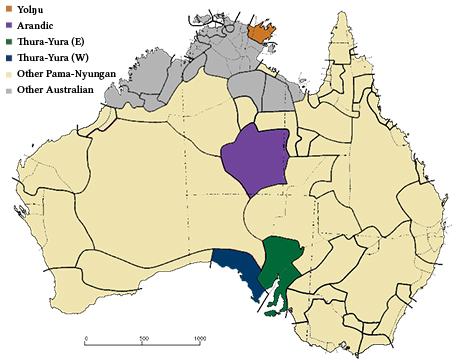
\includegraphics[scale=.7]{YolTYAr-leg.jpg}
	\caption[\textsc{map.} Pama-Nyungan subgroups investigated in Part \ref{NEC}]{Subgrouping of Australian languages. Pama-Nyungan family in tan, with Yolŋu subgroup given in ochre, Arandic in purple and Thura-Yura divided into green (Eastern varieties) and blue (Western/Nangga varieties.)}\label{Map}
\end{figure}

 Strategies that natural languages deploy to mark negation have long attracted the attention of philosophers and linguists \citep[see][]{Horn1989,Horn2010}. In a comprehensive piece of work on the subject, \citet[xiii--xiv]{Horn1989} observes that the ‘simplicity and transparency’ of logical negation (\textit{i.e.}, that function which ``reverses'' the truth value of a given proposition) is not recapitulated in ordinary language, where the complex behaviour of markers of negation and their interaction with other linguistic categories have long been investigated.\footnote{For \citet[1]{Horn2017}, \textit{negation} is basically the phenomenon of ``semantical opposition'' -- we are interested in that function which ``relates an expression $ e $ to another expression with a meaning that is in some way opposed to the meaning of $ e $.''}


 Recent work in the functionalist tradition (\citealp[\textit{e.g.},][]{Miestamo2005} a.o.) has sought to propose a typology for the behavior of `standard negation' marking strategies across a sample of world languages (including 40 Australian varieties.) \textit{\Acrfull{sn}} is understood as those language-specific mechanisms whose function is the inversion of the truth value of a proposition associated with a given (declarative) clause. Drawing a distinction between \acrshort{sn} and `special negation' is warranted in view of the empirical fact that many languages have distinct formal mechanisms for the negation of nonverbal (\textit{e.g.}, copular, existential) predications, imperatives and other types of `subclausal' negation \citep{Miestamo2007,Horn2017,Veselinova2013,VanderAuwera2005}.
\subsection{Negation \& Australia: a typological snapshot}

Mentioned above, roughly 300 Australian languages have been reconstructed to a single family, Pama-Nyungan, spoken across Australia except for some regions in the north of the continent. The most recent common ancestor of these languages is esimated to have been spoken roughly five to six thousand years \textsc{BP} (a similar timedepth to Indo-European, see \citealt[742]{Bouckaert2018}). Many of these languages remain underdescribed, and consequently, typological and comparative work detailing the expression of negation across Australian languages is underdeveloped. Exceptions to this include \citealp{Dixon2002a} and \citealt{Phillips2021b}, surveys that have turned up some generalisations about the formal and functional expression of negation in these languages. Based on the insights of these works, we might divide the `negative semantic space' so to distinguish four macro-categories of negator: (1) negative imperatives/prohibitives, (2) clausal/standard negators and (3) nominal negators, including specialised negative existentials and a commonly occurring `privative' category, and (4) negative interjections. There is a substantial amount of variation in the formal exponence of each of these functions, some varieties distinguishing all four categories  (\textit{e.g.}, Bidjara [\gls{bym}]), some with a single syncretic marker for all four (e.g. Dyirbal [\gls{dbl}], according to \citealp[84--table 3.3]{Dixon2002a}). 

An exceptionful (but otherwise fairly robust) formal tendency across Australian languages is for clausal negation to be marked with a particle pre-verbally and for privative case to be encoded as a nominal suffix. We will explore the implications of this generalisation and its exceptions below, in a general overview of negation strategies in Australia, in addition to a deeper discussion of the meaning contribution of the so-called ``privative case'' markers in Australian languages. %The remainder of this section constitutes a brief survey the exponence of negation strategies in Australian languages, partially summarising insights from \citeauthor{PhillipsFCb} (forthcoming).
\subsection{``Standard'' negation}
This subection briefly provides some generalisations about clausal negation strategies in Australian languages. For a more comprehensive discussion of exceptions and significant interactions between \acrshort{sn} and other aspects of the verbal complex in Australian languages, the reader is referred to \citealt{Phillips2021b}.

\citet[82]{Dixon2002a} claims that ``almost every Australian language marks `not' by a non-inflecting particle which goes before the verb.'' He notes explicitly that this generalisation extends also to the most morphologically synthetic non-Pama-Nyungan languages spoken in the north of the continent. Negation in the Arandic subgroup of Pama-Nyungan, which provides a major exception (one of few) to this formal generalisation, and is particularly relevant for current purposes, is discussed in more detail in §\ref{ar}. The data from Nakkara ([\gls{nck}] Arnhem, Maningrida, \citealt[191]{Eather2011}) and Ngiyambaa ([\gls{wyb}] Pama-Nyungan: Wiradhuric) below clearly demonstrate this generalisation. In Nakkara (\getref{sn-nck}), a preverbal negative marker \textit{korla} takes scope over a fully inflected verbal predicate (also affecting the inflectional suffix licensed by the verb, see also Ch. \ref{yolŋu} below.)
Further, in Ngiyambaa (\getfullref{sn-wyb.wyb1}), the preverbal SN particle \textit{waŋaːy} takes scope over the entire sentence (crucially including the discourse anaphor \textit{yingalaːdhi-} `because of that'), whereas it scopes underneath this item, over only the second predicate in (b), yielding two distinct propositions. 

\pex\begingl\glpreamble \textsb{Preverbal standard negation in Nakkara}\trailingcitation{\citep[191]{Eather2011}} \deftagex{sn-nck}//
\gla \textbf{Korla} nga-y-bburda-ma.//
\glb \textsc{\textbf{neg}} 1s.\gls{erg}-\gls{irr}-hit-\gls{infl}.\textsc{neg}//
\glft`I didn't hit him.'//\endgl\xe
\pex\deftagex{sn-wyb}\textsb{ Preverbal standard negation in Ngiyambaa}\trailingcitation{\citep[239]{Donaldson1980}}
\a\deftaglabel{wyb1}\begingl\gla \textbf{Waŋaːy} yiŋgalaː-dhi\textdblhyphen dju\textdblhyphen na girimiyi-la.//
\glb \textsc{\textbf{neg}} same-\textsc{circ}\textdblhyphen 1.\textsc{nom}\textdblhyphen3.\textsc{abs} wake\textsc{.pst-then}//
\glft`It wasn't because of that I woke her then.'//\endgl

\a\label{wyb2}\begingl\gla Yiŋgalaː-dhi\textdblhyphen dju\textdblhyphen na \textbf{waŋaːy} girimiyi-la.//
\glb same-\textsc{circ}\textdblhyphen 1.\gls{nom}\textdblhyphen3.\gls{abs} \textbf{\gls{neg}} wake.\gls{pst}-then//
\glft`Because of that I didn't wake her then.'//\endgl
\xe
\subsection{The ``privative case'' and existential predications}\label{priv-sems}

The privative case (\gls{priv}) is a very robustly attested category in Australian languages \citep[84]{Dixon2002a}.\footnote{Morphological cases with similar semantics are referred to as \textit{abessive} and/or \textit{caritive} in other literatures \citep[\textit{e.g.} for Uralic in][]{Hamari2011,Hamari2015,Tamm2015}. `Privative' is ubiquitous in Australian language description and will be used here throughout.} Broadly speaking, it predicates the absence of some property denoted by the noun that it associates with, although the precise semantic domain of this category varies considerably across languages \citep[\textit{cf.} arguments for the predicative status of negative existential markers in ][139]{Veselinova2013}. In Nyangumarta (\gls{nna} Pama-Nyungan: Marrngu), for example, \textit{-majirri} `\gls{priv}' can be used to predicate absence (\textit{i.e.} as a negative existential, see (\getref{nna-privEx}). Muruwari (\gls{zmu} Pama-Nyungan: SE) similarly makes use of a form \textit{-kil\textasciitilde-til\textasciitilde-tjil}, shown in (\getfullref{zmu-privEx}{a-b}).\footnote{Incidentally, \citet[77]{Oates1988} describes this suffix as the \textsc{abessive}: ``the opposite of the comitative in that it signifies `lacking' or `being without' some person of thing.' She glosses it throughout as `lacking.'}
\gls{priv} case markers are frequently antonymous to another case suffix --- also often-occurring in Australian languages --- usually glossed as the comitative (\gls{comit}), proprietive (\gls{prop}) or `\textit{having}' case. Uses of this marker are given in (\getref{ComEx}). The apparent synonymy of (\getref{zmu-privEx}b) and (\getref{ComEx}b) demonstrate the antonymous relation between comitative and privative predications.\footnote{The appendix to \citet{Singerman2018} comments on the instantiation of a very similar distribution in Tuparí ([\gls{tpr}] Tupian: NW Brazil), where the suffix \textit{-psiro} \textsc{`have'} is antonymous to \gls{priv} uses of the suffix \textit{-'om} `\gls{neg}'. }
%This function is clarified when contrasted against the `comitative/proprietive', another frequently occurring morpheme.


\pex Function of \textit{-majirri} `\gls{priv}' in Nyangumarta\deftagex{nna-privEx}\trailingcitation{\citep[140]{Sharp2004}}
\a\begingl\gla mungka-\textbf{majirri} karru-\textbf{majirri}-pa paru-\textbf{majirri} jungka jakun\deftaglabel{jungka}//
\glb tree\textbf{-\gls{priv}} stream\textbf{-\gls{priv}}-\gls{conj} spinifex\textsc{-\textbf{priv}} ground only//
\glft`There were no trees, creeks, or spinifex; only the ground (in that country.)'//\endgl
\a\begingl\gla mirtawa mayi-\textbf{majirri}\deftaglabel{mirtawa}//
\glb woman vegetable-\textbf{\gls{priv}}//
\glft`The woman is without food'//\endgl\xe
\pex~Function of \textit{-kil} `\gls{priv}' in Muruwarii\trailingcitation{\citep[77-8]{Oates1988} }
\a\begingl\gla palanj mathan\textbf{-kil}//
\glb nothing stick\textbf{-\gls{priv}}//
\glft`(There are no) sticks [...nothing]'//\endgl
\deftagex{zmu-privEx}
\a\begingl\gla ngapa\textbf{-kil}-pu-n//
\glb water-\textbf{\gls{priv}}-3\gls{s}-\gls{nmlzr}//
\glft`He has no water.' (lit. `he-waterless')// \endgl
 \xe
\pex~Existential function of Muruwari \textit{-piɾa, -yita `\gls{comit}'} \trailingcitation{\citep[73-4]{Oates1988}}
	\deftagex{ComEx}
\a\begingl%\glpreamble }//
	\gla thuu kuya-\textbf{yita} wartu//
	\glb much fish-\textsc{\textbf{comit}} hole.\gls{abs}//
	\glft`The river has a lot of fish in it.' (= `There's a lot of fish in the river')//\endgl
	\a\begingl\gla wala mathan-\textbf{piɾa}//
	\glb \gls{neg} limb-\textbf{\gls{comit}}//
	\glft`(There are) no sticks.'//\endgl
\xe




Australian languages have a number of strategies to express existential and non-exis\-tence (absence) predications. (\getfullref{nna-privEx}) shows the Nyangumarta privative marker functioning as an existential negator: it predicates the absence of trees, streams and spinifex (a culturally important tussock grass) of a particular location. Additionally, \textit{contra} a prediction made by \citet[19]{Croft1991}, it is the case in many Australian languages that ``an existential sentence [can] consist solely of the noun phrase whose existence is predicated.'' Additionally, (\getfullref{nna-privEx}) includes an example of bare NP existential predication; the presence of \textit{jungka} `[bare] ground' (in the relevant location) is predicated.\footnote{Such constructions have also been reported elsewhere in the literature, \textit{e.g.}, for Māori [\gls{mao}] where ```existence'' statements have no copula or existence verbs' (\citealp[78]{Bauer1993}, cited by \citealp{Chung2004} a.o). Similarly, sign languages tend to allow bare-NP existential predication (see \citealt[26ff]{deWeert2016} on Flemish and Finnish sign languages.). Even Marra [\gls{mec}] (a language cited in \citealt[14]{Croft1991}) appears to permit bare NP existentials, if Heath's \citeyearpar[364]{Heath1981} translations are to be trusted.}
 These facts immediately present a challenge to the (formal) negative existential cycle as formulated: if existence predicates are frequently verbless, there is no way to formally distinguish between NEC stages $ \boldsymbol{\mathbb{A}} $ and $ \boldsymbol{\mathbb{C}} $ on the basis of synchronic data. I know of no Australian language with a \textit{reserved} existential verb; like copular clauses, existence predications appear to frequently make use of a stance or motion verb (most frequently one that primarily means `sit' or `lie' and often polysemous with `stay, live'), or are otherwise verbless.\footnote{Notable, however, is the fact that these stance/motion verbs often lend particular semantic nuances to the copular and existential predications in which they participate \citep[see e.g. ][610-611]{Wilkinson1991}.}

Relevantly for current purposes, then, the semantics of the privative suffix in this nonexistential use can be instructively captured by adapting existing analyses of existential propositions \citep[\textit{e.g.},][]{Francez2007,McNally2016}. These analyses generally characterise existential predication as comprising \textbf{obligatorily} some (type of) entity whose existence is being predicated (known as the \textsc{pivot)} and some \textbf{optional} restriction (perhaps locative) on its existence \citep[the \textsc{coda}; see][]{Francez2007}. Adapting Francez's analysis would mean treating privative noun phrases as generalised quantifiers of nonexistence. This is consonant with Croft's \citeyearpar[18]{Croft1991} observation about the privileged status of existential predication: representable as a logical quantifier as opposed to the one-place predicates of other stative verbs. For Croft, the relevant semantic distinction is that, where statives predicate a \textit{property} of a given individual, existentials are taken to ``[indicate] the presence or absence of the object itself.''  This observation --- an apparent conceptual distinction between the negation of a property versus the negation of existence --- forms the basis of functionalist explanation of the ``constant renewal'' of negative existentials at stage $\mathbb{B}$ of the NEC (see also \citealt[173]{Veselinova2016}).


In (\getref{Qdet}), I adapt Francez's quantificational treatment of existential predication in order to give a semantics for \textsc{priv} \citep{Francez2007,McNally2011}. Effectively, privative forms are taken to instantiate a negative quantificational determiner; they assert that the intersection of the two sets of individuals $ (P,\,Q\in\mathfrak D_{\langle e,t\rangle} )$ represented by their arguments is empty (\citealp[169]{Barwise1981}).

\pex \textbf{\gls{priv} realises a negative quantifier}
\deftagex{Qdet}\a$\textbf{no}=\lambda P_{\langle e,t\rangle}\lambda Q_{\langle e,t\rangle}.P\cap Q=\varnothing$%\hfill{\citep[i.e.,][169]{Barwise1981}}
\a $\llbracket\textsc{priv}\rrbracket=\lambda P_{\langle e,t\rangle}\lambda Q_{\langle e,t\rangle}.\textbf{no}(P,Q)$\xe


$ P $ and $ Q $ respectively represent those properties that can serve as the ``pivot'' and ``coda'' of an existential predication. Crucially $ Q $ need not have any syntactic representation, but is rather derived from context indexically (see \getfullref{nna-privEx.jungka}). This process, --- Francez's ``contextual closure'' \citeyearpar[72]{Francez2007}) --- is spelled out in (\getref{mungka}) below. Effectively, the variable $ Q $ over sets of individuals is saturated by a contextually given relation and discourse entity/set of parameters (\getref{francez-cc}).

\pex \textbf{Contextual domains of entities} \citep[from][71]{Francez2007}\deftagex{francez-cc}

For any element $ \alpha\in\mathfrak D_\tau$, $ \alpha $'s contextual domain is given as:
$$ d_\alpha\underset{\text{def}}{=} \lambda y_{\tau'}[\mathcal R_{\langle\tau,\langle\tau',t\rangle\rangle}(\alpha,y)]$$
That is, the set of individuals $ y\in\mathfrak D_{\tau'} $ that are related to $ \alpha_\tau $ by some pragmatically-inferred relation $ \mathcal R\subseteq \mathfrak{D_\tau\times\wp{(D_{\tau'})}} $

\xe

\noindent $ \mathcal R $ might be associated, for example with some relation \textbf{loc} which takes a set of salient spatiotemporal parameters (Francez suggests that this might be represented as a tuple $ st=\langle t,\ell\rangle $ and maps these to some set of entites \textbf{loc}ated within $ st $ (at that place, at that time.))

For Francez, the \textsc{coda}, then, plays the role of a ``contextual modifier'', the same type as a frame adverbial. In effect, it serves to explicitly provide that entity whose contextual domain satisfies $ Q $ (78). For example, in (\getfullref{nna-privEx.mirtawa}), the privative phrase is contextually ``closed'' by $ d_{\textit{mirtawa}} $ --- some set of things related (perhaps possessed) by \textit{mirtawa} `the woman.'


A truth-conditional analysis of one privative-marked noun (\textit{mungka} `tree') from (\getfullref{nna-privEx.jungka}) is provided in (\getref{mungka}) below; each step is spelled out in prose.

\pex \textbf{`There were no trees (in that country)': deriving (\getfullref{nna-privEx.jungka})}
\a\begingl\gla mungka-majirri//
\glb tree-\textsc{priv}//
\endgl
\a $\denote{\textit{mungka}}_{\langle e,t\rangle} =\lambda x_e.\textsf{Tree}(x) $
\a $\denote{\textit{mungka-majirri}}_{\langle\langle e,t\rangle,t\rangle}=\lambda Q_{\langle e,t\rangle}\big[\textbf{no}(\lambda x[\mathsf{Tree}(x)],Q)\big]$\label{privsemsF}\\
The privative-marked NP \textit{mungka-majirri} `tree-\gls{priv}' is a generalised quantifier: it states that there exists nothing in the domain in the intersection of the set of trees $(\lambda x.\textsf{Tree}(x))$ and some other property $ Q $ (which will be provided by the context of utterance, \textit{sc.} Francez's \textit{contextual domain} $d_\alpha$ \citeyearpar[71]{Francez2007}).
\a\textsb{Contextual closure}\par\nobreak

$\begin{aligned}\denote[c]{\textit{mungka-majirri}}&=\textbf{no}\big(\lambda x[\textsf{Tree}(x)],d_\alpha\big)\\
%&=\textbf{no}(\lambda x[\textbf{Tree}(x)],\lambda y[\textbf{loc}(st_c,y)])\\
&=\textbf{no}\big(\lambda x[\textsf{Tree}(x)],\lambda y[\textbf{loc}(st_c,y)]\big)\\\end{aligned}$\\
$ \boldsymbol Q $ is then saturated by $ d_{st_c} $: the ``set of things related [...] to the spatiotemporal parameters'' being predicated of (\textit{viz.} those things related to a particular patch of \textit{warrarn} `country' in the past, per Sharp's translation in (\getfullref{nna-privEx.jungka})) \hfill $ d_{st_{c}}=\lambda y_e.\mathcal R(\textsf{`that country'},y)$\deftagex{mungka}\deftaglabel{closure}

\xe

As (\getfullref{mungka.closure}) makes clear, in the absence of an explicit/linguistically-encoded ``coda'' to serve as a locus/restrictor for the privative predication, the \textbf{context} of utterance has made available an additional restriction ($ d_\alpha $) as the second argument to \textbf{no}. This restriction may take the form of a function \textbf{loc}, which returns that set of things that are taken to be related to whichever salient spatiotemporal parameters the context provides.


\subsection{Privatives and the \acrshort{NEC}}

If we treat the privative marking on NPs as a type of negative existential predicate, a consequence of the \acrshort{NEC} is the prediction that these markers ought to eventually generalise, displacing an erstwhile standard negator (\textit{i.e.}, \gls{priv}  markers will participate in the \acrshort{NEC}.) Phonological identity between privatives and SN is indeed well-attested in Australia (\textit{e.g.}, in Bardi [\gls{bcj}] \citep{Bowern2012} and Warrongo [\gls{wrg}] \citep{Tsunoda2011}). In these languages, negative existential/privative predication may be syntactically distinguished from standard clausal negation by placing the general \gls{neg} particle post-nominally instead of preverbally (shown in (\ref{wrg-exx}), in addition to 3456(\ref{wgu-exx}a--b) below.)

\pex \textbf{Negation in Warrongo} (\texttt{[wgu]} Pama-Nyungan: Maric)\label{wrg-exx}
\a\begingl\glpreamble Senential negation with initial \textit{nyawa} `\textsc{neg}'//
\gla \textbf{nyawa} ngaya balga-lgo banjo-lgo.//
\glb \textsc{\textbf{neg}} 1\gls{s}.\gls{erg} hit-\gls{purp} ask\textsc{-purp}//
\glft`I will not hit [him]. [I] will ask [him].'\trailingcitation{\citep[363]{Tsunoda2011}}//\endgl

\a\begingl\glpreamble Existential negation with postnominal \textit{nyawa} `\gls{neg}'//
\gla nyawa, yarro walwa yamba. + yori \textbf{nyawa}, gajarra \textit{\textbf{nyawa}} worriba \textbf{nyawa}, barrbira \textbf{\textit{nyawa}}, jagay \textbf{\textit{nyawa}}.//
\glb \textsc{neg} this bad country. kangaroo \textsc{\textbf{neg}}, possum \textbf{\gls{neg}} sugarbag.bee \textbf{\gls{neg}} echinda \textbf{\gls{neg}} sand.goanna \textbf{\gls{neg}}//
\glft`No, this country is no good. There are no kangaroos, no possums, no bees, no echidnas, no sand goannas [in my country].'\trailingcitation{\citep[661]{Tsunoda2011}}//\endgl
\xe

 A possible example of a postnominal existential negator acquiring the function of clause-initial standard negator is found in Wirangu (\texttt{[wgu]} Pama-Nyungan: Thura-Yura). This scenario is described in \S~\ref{TY} below, along with a discussion of its potential import for theories of the \acrshort{NEC}.

\section{Negative domains \& the \acrshort{NEC} in three Pama-Nyungan subgroups}\label{empirical}

In this section, comparative and langauge-internal data from three subgroups of Pama-Nyungan, as they relate to the \acrlong{NEC}, are investigated.

§~\ref{TY} comprises a discussion of Thura-Yura --- a family spoken along the South Australian coast. In Thura-Yura, we observe a likely trajectory where a suffixal privative form appears to have developed into a preverbal standard negator \textit{maga}. In Wirangu, this has change created the conditions for the recruitment-by-borrowing of lexical material from an unrelated neighbouring language as a new privative.

§~\ref{NEC-yolŋu} consideres data from Yolŋu Matha, a family spoken in Eastern Arnhem Land. This section considers the competition and structured variation between two markers, \textit{yaka} and \textit{bäyŋu} --- the latter previously having been restricted to `negative quantifier' functions. In addition to this, we consider comparative evidence which suggests that in Djambarrpuyŋu privative marker \textit{-miriw} has expanded out of its traditional domain, to the extent that it is now showing signs of also being in competition with the preverbal negative particles. Conversely, the Ritharrŋu data show how a distinct sentential negative suffix \textit{-ˀmayˀ} appears to have been borrowed from a neighbouring language; a finding not predicted by (unidirectional) accounts of the NƎC.

Finally, §~\ref{ar} examines \acrlong{sn} as realised by negative suffixation in Arrernte; a typologically unusual feature for Australian languages. It is shown that negated clauses in Arrernte are actually derived (de-verbal) nominal predicates. This fact of Arrernte appears to provide strong evidence in favour of a trajectory where the standard negation strategy in this language is an erstwhile privative (negative existential) marker \textit{-tye\textdblhyphen kenhe} that has completely displaced an older form (and then triggered the recruitment of a new special negator for negative existential predications \textit{-kwenye}).




\subsection{Thura-Yura: change \& renewal in the negative domain}\label{TY}

Thura-Yura is a Pama-Nyungan language family, with nine documented varieties historically centered on and around the South Australian coast. The Western varieties of these languages abut the Wati (Western Desert) family. Figure \ref{TY-tree} describes the familial relations of the described Thura-Yura languages whereas Table \ref{TYdata} compares their negative lexica (including a possible reconstruction.) Examples of Wirangu negative predications are given in (\ref{wgu-exx}) below.\footnote{Note that \citep[57]{Hercus1999} describes a number of other markers with negative import in her Thura-Yura grammar (including two other lesser-used privatives, which she regards as older. \textit{Cf.} Veselinova's \citeyearpar[173]{Veselinova2016} ``constant renewal of the negative existentials.''}



	\begin{figure}[h]\centering
		\caption[\textsc{phylogeny.} Subgrouping in Thura-Yura]{A selection of the internal structure of the Thura-Yura family (spoken in South Australia) following \citealt[183]{Simpson2004}. \textit{Nangga} is the name given to the Western subgroup whereas core-ThuraYura refers to the Eastern varieties (see Figure \ref{Map} above for the approximate geographic distribution.)}\label{TY-tree}\small
	\begin{tikzpicture}
	\tikzset{edge from parent/.style=
{draw,
edge from parent path={(\tikzparentnode.south)
-- +(0,-8pt)
-| (\tikzchildnode)}}}
\tikzset{frontier/.style={distance from root=130pt}}

	 \Tree [.\textbf{\textit{\textsc{Thura-Yura}}} [.\textit{{\color{Blue}\textbf{Nangga}}} Wirangu Nauo ] [.\textit{{\color{OliveGreen}\textbf{core~TY}}} Nukunu  [.\textit{Yura} [Adnyamathanha Kuyani ] Bangarla ] [.\textit{Kadli} ] ] ] 
	\end{tikzpicture}\end{figure}
%\renewcommand{\arraystretch}{1}


Table \ref{TYdata} shows (colour-coded for cognacy) four of the negative-associated lexical items in the Thura-Yura family, each of which will be discussed here. It allows for a probable reconstruction of a standard negator (or nominal negator) \textit{*maka} and/or \acrshort{sn} \textit{*guda} in the ancestral language. Of Wirangu \texttt{[wgu]}, \citet[57]{Hercus1999} claims that privative morpheme \textit{-yudu} has entered the language as a borrowing from the Kokata language, a Western Desert dialect spoken in neighbouring territories to the North ([\gls{ktd}] Pama-Nyungan: Wati). \textit{-yudu} has largely displaced \textit{-maga} as the form of the privative. The recruitment of a distinctive privative form (from lexical resources of a neighbouring, unrelated language) may well be taken as evidence of pressure for the privileged marking of negative existentials that is taken to motivate the beginning of the NƎC (\textit{sc.} stage transition $\mathbb{A\to B}$).

\begin{table}[H]\centering
	\caption[Lexicalisation of the negative domain in Thura-Yura]{Reported partitions in the negative semantic space (data adapted from \citealt{Hercus1999,Hercus1992,Schurmann1844,Hercus1996,Black1917}.) Colouring reflects hypothesised cognacy of lexical items across Thura-Yura. Dashed arrows represent borrowings from neighbouring languages, solid arrows semantic (functional) change.} \label{TYdata}
\begin{tabular}{r|c|c|c}\toprule
\textit{\textsc{\scriptsize(Wa}}\tikzmark{o}{\centering\scriptsize\textit{\textsc{t}}}\textit{\textsc{\scriptsize i)}}	& \gls{negq}/\gls{priv} & \acrshort{sn} & {\small`cannot'/`not yet'} \\ \toprule
Wirangu [\gls{wgu}] & \begin{tabular}[c]{@{}l@{}}\tikzmark{c}{\textit{\textcolor{teal}{-yudu}}}\\ \textcolor{violet}{\textit{-maga}}\tikzmark{d}\end{tabular}   & \tikzmark{b}\textcolor{violet}{\textit{maga}}   & \textcolor{brown}{\textit{guda}}   \\ \midrule
Nauo [\gls{nwo}] & ? & \textcolor{violet}{\textit{makka}} & \\\midrule
Bangarla [\gls{bjb}] & \textcolor{violet}{\textit{-maga}}  & \textcolor{violet}{\textit{makka}}  & \tikzmark{a} \textcolor{brown}{\textit{kutta}}\\ \midrule
\begin{tabular}[c]{@{}r@{}}Adnyamathanha [\gls{adt}]\\Kuyani  [\gls{gvy}]\end{tabular} & \tikzmark{pari}{\textit{pari- }}  & \textcolor{brown}{\textit{(g)uda}}   & \tikzmark{e}--\tikzmark{ee}   \\\midrule
Nukunu [\gls{nnv}] & \textcolor{violet}{\textit{-wakanha}$ ^? $} & & \\\midrule
\textit{proto-TY} & \multicolumn{3}{c}{\textit{\textcolor{violet}{\textbf{*maka}}/\textcolor{brown}{\textbf{*guda}}}} \\\bottomrule
{\scriptsize{\textcolor{gray}{\textit{\textsc{Diyari?}} ([\gls{dif}] Karnic)}}}\tikzmark{dif}
\end{tabular}

\begin{tikzpicture}[overlay,remember picture, shorten >=1pt]
\draw[->,yshift=3ex,xshift=1ex, color=teal,dashed] (pic cs:o) to[bend right] (pic cs:c) ;
\draw[->,xshift=-3ex,yshift=.5ex, color=violet] (pic cs:d) -- (pic cs:b);
%\draw[->,xshift=0.7ex] (pic cs:ee) -- (pic cs:b);
\draw[->,color=gray,dashed,out=0,in=180] (pic cs:dif) to[] (pic cs:pari);
\end{tikzpicture}\end{table}

%%%% THIS IS THE ORIGINAL SUBFIGURE FORMAT THAT REVIEWER X HAS SOME PROBLEM WITH.
%\begin{figure}[h]
%	\caption{Change in the negation domain across Thura-Yura languages}\label{TY-data}
%	\begin{subfigure}{.4\textwidth}
%		\caption{A selection of the internal structure of the Thura-Yura family (spoken in South Australia) following \citealt[183]{Simpson2004}}.\small
%		\Tree [.\textbf{\textit{Thura-Yura}} [.\textit{Nangga} \gls{wgu} \gls{nwo} ] [.\textit{core~TY} [.\gls{nnv} ] [.\textit{Yura} [\gls{adt} \gls{gvy} ] \gls{bjb} ] [.\textit{Kadli} ] ] ] 
%	\end{subfigure}
%	%\renewcommand{\arraystretch}{1}
%	\begin{subfigure}{.5\textwidth}
%		\caption{Reported partitions in the negative semantic space (data adapted from \citealt{Hercus1999,Hercus1992,Schurmann1844,Hercus1996,Black1817}.) Colouring to reflect hypothesised cognacy of lexical items across Thura-Yura.} \label{TYdata}
%		\begin{tabular}{r|c|c|c}\toprule
%			\tikzmark{o}	& \textsc{negq/priv} & SN & {\small`cannot'/`not yet'} \\ \toprule
%			Wirangu [\gls{wgu}] & \tikzmark{c}\begin{tabular}[c]{@{}l@{}}\textit{\textcolor{teal}{-yudu}}\\ \textcolor{violet}{\textit{-maga}}\tikzmark{d}\end{tabular}   & \tikzmark{b}\textcolor{violet}{\textit{-maga}}   & \textcolor{brown}{\textit{guda}}   \\ \midrule
%			Nauo [\gls{nwo}] & ? & \textcolor{violet}{\textit{makka}} & \\\midrule
%			Bangarla [\gls{bjb}] & \textcolor{violet}{\textit{-maga}}  & \textcolor{violet}{\textit{makka}}  & \tikzmark{a} \textcolor{brown}{\textit{kutta}}\\ \midrule
%			\begin{tabular}[c]{@{}r@{}}Adnyamathanha [\gls{adt}]\\Kuyani  [\gls{gvy}]\end{tabular} & \textit{pari- }  & \textcolor{brown}{\textit{(g)uda}}   & \tikzmark{e}--\tikzmark{ee}   \\\midrule
%			Nukunu [\gls{nnv}] & \textcolor{violet}{\textit{-wakanha}} & & \\\midrule
%			\textit{proto-TY} & \multicolumn{3}{c}{\textit{\textcolor{violet}{\textbf{*maka}}/\textcolor{brown}{\textbf{*guda}}}} \\\bottomrule
%		\end{tabular}
%		
%		\begin{tikzpicture}[overlay,remember picture, shorten >=1pt]
%		\draw[->,yshift=2ex,xshift=-1.5ex] (pic cs:o) -- (pic cs:c) ;
%		\draw[->,xshift=0ex,yshift=.5ex] (pic cs:d) -- (pic cs:b);
%		%\draw[->,xshift=0.7ex] (pic cs:ee) -- (pic cs:b);
%		\end{tikzpicture}\end{subfigure}\end{figure}





\pex \textbf{Examples of Wirangu negation strategies (from \citealt{Hercus1999})}\label{wgu-exx}
\a\begingl\glpreamble \textit{maga} SN//
\gla Warlba marnaardu-nga \textbf{maga} wina-rn!//
\glb wind big\textsc{-loc} \textsc{\textbf{neg}} go\textsc{-pres}//
\glft `(I am) not going out in a gale!'\trailingcitation{(142)}//\endgl

\a\begingl\glpreamble \textit{-maga} privative//
\gla Nganha gidya\textbf{-maga}//
\glb 1\gls{s} child-\textsc{\textbf{priv}}//
\glft`I haven't got any children.'\trailingcitation{(57)}//\endgl

\a\begingl
\glpreamble \textit{-yudu} privative (``most commonly used'')//
\gla Nganha barnda-\textbf{yudu}//
\glb 1\gls{s} money-\textsc{\textbf{priv}}//
\glft`I haven't got any money.'\trailingcitation{(57)}//\endgl

\a\begingl\glpreamble \textit{guda} SN (modalised)//
\gla Ngadhu \textbf{guda} wangga-rn//
\glb 1\gls{s}.\textsc{erg} \textsc{\textbf{neg.}irr} speak\textsc{-pres}//
\glft`I can't talk (about this; it's too embarassing.)'\trailingcitation{(143)}//\endgl
\xe


 Similarly, Adnyamathanha [\gls{adt}] and Kuyani [\gls{gvy}] have recruited \textit{pari-} as a negative existential/predicator of absence \citep[141]{Hercus1999}. This may also be a borrowing from the Karnic lanugages that abut Eastern Thura-Yura (e.g. Diyari [\gls{dif}] \textit{pani} \textsc{`priv'}, (\citealt{Austin2011}, {C. Bowern \textit{p.c.}).\footnote{This remains to be demonstrated, but \textit{pari-} may otherwise be cognate with Wirangu \textit{bal-} `die,' elsewhere described as a lexical source for negators (\citealt{Veselinova2013}, van Gelderen this volume). An argument potentially in favour of this is found in a possibility of an example of lexical renewal likely born of euphemism; Adnyamanthana \textit{inta-} `die' appears to be cognate with Wirangu \textit{inda-} `spill.'}
\textit{maga} retains its function as the primary standard negator particle in Wirangu (and Bangarla [\gls{bjb}]),  whereas \textit{guda} (the standard negator in Adnyamathanha and Kuyani), is restricted to a subset of negative meanings: `cannot' and `not yet' (note that, particularly in northern Australia, the form of negative marking is often conditioned by speaker mood/reality status (see Part \ref{yolŋu}, esp. \S~\ref{sec:yol-mood} for an example of a related phenomenon.)

A potential cognate in the southern Thura-Yura (Kadli) language, Kaurna [\gls{zku}] (not represented in Figure \ref{TY} for a lack of available data) \textit{wakka-} is found (possibly fossilised) in lexical items \textit{wakkarendi} `err, stray, be lost', \textit{wakkariapendi}, `forget, not think of, leave behind', \textit{wakkariburka} `ignorant person, simpleton' \citep[II-52]{Schurmann1840}.\footnote{Note attested stems in \textit{pia\textbf{-rendi}} `scattered, stray', \textit{pia\textbf{-riappendi}} `scatter, disperse', \textit{\textbf{burka}} `adult, man' \citep[II-4,38]{Schurmann1840}.} All three of these words appear to be analysable; \textit{wakka-} contributing some notion of emptiness, characteristic of an erstwhile nominal negator/privative category. Apparently, \citeauthor{Teichelmann1840} (1840, cited in \citealt{Amery1996a}) give \textit{mukandariappendi} as the form for `forget' --- support for potential \textit{m\textasciitilde{w}} alternation and the cognacy of these forms.\footnote{Data for Kaurna (and other extinct varieties) is scarce, effectively limited to the lexica published by nineteenth-century missionaries, \citet{Schurmann1840}. A possible reflex of \textit{*guda} is found in items like \textit{kudmunna} `ignorant, not knowing' (II-12). Additionally, Narungga \textit{-gu} (potentially a ``compound form'') appears in a number of words with a meaning akin to `blocked', according to \citet[82]{Eira2010}. Notably, compare \textit{mina-gu} `blind' (lit. `eye-blocked') where the semantic connection to an inability/impossibility reading is clear.
	
	Other negative lexical items reported here are \textit{yakko} which appears to function as a SN marker and \textit{-tinna} which is given as the most frequent form of `without' (i.e. the privative.)}

 There are insufficient available data to adjudicate between competing hypotheses that (a) \textit{*guda} has been largely displaced by erstwhile nominal negator \textit{maga} in Wirangu or (b) \textit{guda} has replaced \textit{*maka} in Adnyamathana/Kuyani. Nevertheless, an analysis informed by the insights of the \acrshort{NEC} favours and supports (a).
 
Under such an analysis, Wirangu -- the Thura-Yura outlier -- provides a particularly clear example of a language, the negator forms of which are transitioning through the NEC. The erstwhile negative existential \textit{-maga} has entered the domain of standard, clausal negation, adopting the morphosyntactic properties of a preverbal negative (stage $\mathbb{B\to C}$),\footnote{Note that, while this change is consonant with functional grammaticalisation ``generalisation'', the transition from bound- to free-form is perhaps surprising in view of the (controversial) claim that grammaticalisation clines involve processes of phonetic reduction and syntactic ``rigidification'' (e.g. \citealp{Geurts2000}). If the account described here is on the right track, the trajectory of \textit{maga} in Wirangu constitutes a counterexample of these grammaticalization ``form'' paths (see \citealp[40]{vanderAuwera2008,Ahern} for the dissociation of ``formal'' and ``functional/semantic'' grammaticalisation processes).} and triggering the recruitment of a new privative marker from the lexical resources of a neighbouring language \textit{-yudu} which is now in competition with the old marker (stage $\mathbb{A\to B}$). The ostensible simultaneity of these changes also provides further evidence for competition between functional and formal pressures for generalisation and recruitment (\textit{sc.} Veselinova's ``constant renewal of the negative existential'' \citeyearpar[173]{Veselinova2016}).
\citealt[225]{Miestamo2005}, \citealt{Phillips2021b}.)%todo\marginnote{there's sth strange going on w the T\&S sourcing here, i'm not totally sure who says what \& may need to go back to archives to find out.}

Additionally, if the directionality of change described here is indeed on the right track, Wirangu can be shown to resist classification into any unique \acrshort{NEC} `stage', transitional or ``cardinal'' (in which case the \acrshort{NEC} as described in previous work does not represent a complete linguistic typology for negative existential marking strategies.)\footnote{The issues of ``assigning'' the entire negative domain of a given language to a unique stage in the \acrshort{NEC} have been explored in some detail by \citep{Veselinova2016}, who observes similar classificatory issues for a number of languages (\textit{e.g.}, East Futunan [\texttt{fud}]: Polynesian).}










\subsection{The Yolŋu negative domain}\label{NEC-yolŋu}

The Yolŋu languages, a Pama-Nyungan grouping of at least six dialect clusters (roughly coterminous with sociocultural groupings) are spoken through Eastern Arnhem Land (in the far north of the continent) by some 12,000 Aboriginal inhabitants (see Part \ref{yolŋu} of the current dissertation, also \citealt[18\textit{ff}]{Wilkinson1991}). Yolŋu are strictly exogamous -- each cultural group (clan) being associated with a distinct dialect, a situation that has led to a significant amount of stable linguistic variation (and, consequently, undetermined internal classification; see \S~\ref{sec:yol-bkgrd}, also  \citealt{Schebeck2001}, \citealt[836]{Bowern2012b}).
%todo intro ch for more ym

This section compares the negation systems of three distinct Yolŋu varieties: Djambarrpuyŋu [\gls{djr}], Ritharrŋu [\gls{rit}] and Wangurri [\gls{dhg}] in view of making inferences about change in marking strategies over time. A pattern similar to that observed in Thura-Yura is shown. The key findings are tabulated in Table \ref{compYol} below. The final subsection (§\thinspace\ref{yolpriv}) comprises a discussion of privative case semantics with particular reference to Yolŋu.

\begin{table}[h]
	\centering
	\caption[Lexicalisation of the negative domain in three Yolŋu Matha varieties]{Partitioning of the negative space in three Yolŋu languages.\\`\gls{proh}' negates imperatives, \gls{sn} represents `standard negation'. `\gls{priv}' is taken to denote a suffix of the type described above. `\gls{negq}' (Wilkinson's ``negative quantifier'') are independent words that appear to quantify over the NP which they modify (\textit{i.e.}, perform (minimally) the same work as a \gls{priv} suffix.)}
	\label{compYol}
	\begin{tabular}{lrllll}
		&& {\sc proh}                                                     & {\sc sn}                                                         & {\sc negq}                                             & {\sc priv} \\\toprule\toprule
		\textbf{Djambarrpuyŋu} & \gls{djr} & \textit{yaka}                                                             & \begin{tabular}[c]{@{}l@{}}\textit{yaka}\\ \textit{bäyŋu}\end{tabular}               & \textit{bäyŋu}                                                     & \textit{-miriw}       \\\midrule
		\textbf{Ritharrŋu} &\gls{rit} & \textit{yaka}                                                             & -\textit{ˀmayˀ}                                                             & \textit{yakaŋu}                                                    & \textit{-miriw}       \\\midrule
		\textbf{Wangurri} &\gls{dhg} & \begin{tabular}[c]{@{}l@{}}\textit{yaka}\\ \textit{ŋangawul}\\ \textit{bayaŋu}\end{tabular} & \begin{tabular}[c]{@{}l@{}}?\textit{yaka}\\\textit{ŋangawul}\\ ?\textit{bayaŋu}\end{tabular} & \begin{tabular}[c]{@{}l@{}}\textit{ŋangawul}\\ \textit{\textit{bayaŋu}}\end{tabular} & \textit{-nharra}  \\\bottomrule   
	\end{tabular}
\end{table}


\subsubsection{Djambarrpuyŋu}\label{sec:nec-djr} \textbf{Djambarrpuyŋu} [\gls{djr}] appears to provide an example of Croft's $\mathbb{B\sim C}$ transitional-stage language. \citet[356]{Wilkinson1991} describes the coexistence of two markers: \textit{yaka} `\gls{neg}' and \textit{bäyŋu} `\gls{negq}' (negative quantifier): claiming that `both occur as propositional negators,' demonstrated in the data in (\nextx) below, from \citet{Wilkinson1991}.

\pex\textbf{\Acrlong{sn} in Djambarrpuyŋu}
\a\begingl\glpreamble \textit{{\em yaka} as (full) clausal negator}//
\gla \textbf{yaka} ŋayi dhu ga ŋutha-n ŋaṉḏi-wal bäpa-wal//
\glb \textsc{\textbf{neg}} 3\gls{s} \textsc{fut} \gls{ipfv}.\gls{I} grow-\textsc{I} mother\textsc{-obl} father\textsc{-obl}//
\glft `They don't grow up with (their) mother and father.'\trailingcitation{\citep[691]{Wilkinson1991}}//
\endgl
\a\begingl\glpreamble \textit{{\em yaka} as negator in attributive (nonverbal) predication}//
\gla \textbf{yaka} dhuwali ŋatha, dhuwali ŋula nhä-n dhuwali botjin//
\glb \textsc{\textbf{neg}} \gls{med} food \gls{med} \textsc{indef} what-\textsc{seq} that poison//
\glft`That isn't food, that's something else, that's poisonous.'\trailingcitation{\citep[560]{Wilkinson1991}}//\endgl
\a\begingl\glpreamble yaka \textit{as negator in possessive construction}//
\gla warrakan limurruŋ \textbf{yaka} dhuwal//
\glb animal 1\gls{p}.\textsc{incl.dat} \textbf{\gls{neg}} \gls{prox}//
\glft`This meat isn't ours/for us.'\trailingcitation{[AW~20190505]}//\deftagex{yaka}\deftaglabel{meat}
\endgl
\a\begingl
\glpreamble\textit{ {\em bäyŋu} as clausal negator}//
\gla \textbf{bäyŋu} ŋarra gäthur ŋorranha manymak-kunha munhawu//
\glb \textsc{\textbf{negq}} 1\gls{s} today lie.\gls{IV} good-\gls{tr}.\gls{IV} night//
\glft `I didn't sleep well last night.'\hfill\citep[357]{Wilkinson1991}//
\endgl\deftagex{djr-yaka}\xe

The distributional difference between these two markers is twofold. According to Wilkinson, \textit{yaka} is ungrammatical in quantificational contexts and \textit{bäyŋu} does not appear in imperative (\textit{i.e.} prohibitive) contexts. It seems, then, likely, that in Djambarrpuyŋu, \textit{bäyŋu}, an erstwhile negative existential has begun to encroach further into the negation space, entering into competition with \textit{yaka}. \textit{bäyŋu}, with reflexes in other Yolŋu languages, derives from (fairly productive) verbal root \textit{bäy-} `leave.'\footnote{Note also that \textit{-\textsc{th}i} `\gls{inch}' derives absence-associated change-of-state readings: \textit{bäy-thi} `be left over/behind'; \textit{bäyŋu-thi} `be/have none, pass~away, die' \citep[378]{Wilkinson1991}. The semantics of this suffix is investigated in \S~\ref{sec:djr-prs}.} Examples of negative existential uses of \textit{bäyŋu} are given in (\nextx) and prohibitive uses of \textit{yaka} in (\anextx).


\pex\deftagex{bayŋu-negq} \textbf{Djambarrpuyŋu negative quantification}
\a\begingl\gla dhipuŋur-nydja \textbf{bäyŋu} guku//
\glb \gls{med}.\gls{abl}-\gls{prom} \textbf{\gls{negq}} honey//
\glft`From this (tree) there's no honey.'\trailingcitation{\citep[554]{Wilkinson1991}}//\endgl

\a\begingl
	\gla (*yaka/)\textbf{bäyŋu} ŋarra-ku gi ŋorri ŋula dhiyal wäŋa-ŋur-nydja//
	\glb \textsc{*neg/\textbf{negq}} 1\gls{s}\textsc{-dat} \gls{ipfv}.\gls{II} lie:\gls{II} \gls{indef} \gls{prox}.\gls{loc} place-\textsc{loc-foc}//
	\glft`I don't have any here' (lit. `at this place lie (are) none of mine')\trailingcitation{\citep[691]{Wilkinson1991}}//
	\endgl
\a\begingl\gla bili ($^\#$yaka/)\textbf{bäyŋu} limurruŋ dhuwal bäwarraṉ//
\glb because \textsc{$^\#$neg/\textbf{negq}} 1\gls{d}.\textsc{incl.dat} \textsc{prox} animal//
\glft\textbf{Intended reading:} `Because there's no meat for us.'\trailingcitation{(\citealp[560]{Wilkinson1991}, infelicity judgment \textsc{aw20190505}, cf. \lastx c)}//\endgl\deftagex{djr-bayŋu}\deftaglabel{meat}
\xe

\noindent Note in particular the (obligatory) contrast in the interpretation of (\getfullref{djr-bayŋu.meat}) as against (\getfullref{yaka.meat}) where the semantics of \textit{bäyŋu} and \textit{yaka} come apart. Only the former is available as a negative quantifier (that is, on the negative existential reading.)


\pex\deftagex{yaka}\begingl\glpreamble\textbf{Djambarrpuyŋu imperative negation (prohibitive, see also §\ref{yolpriv})}//
\gla \textbf{yaka(/*bäyŋu)} waŋi!//
\glb \textsc{\textbf{neg}(/*negq)} talk.\gls{II}//
\glft`Don't talk!'\trailingcitation{\citep[360]{Wilkinson1991}}//\endgl\xe


There are multiple arguments for a reconstruction of \textit{*yaka} `\gls{neg}' to proto-Yolŋu. First is the fact that it is reported as a negative particle in all Yolŋu varieties \citep[31]{Schebeck2001}.

 Secondly, possible lexical cognates are reported in likely sisters to Yolŋu in the Western Pama-Nyungan subfamily (a monophyletic branch reconstructed in \citealt[838]{Bowern2012}). \citet[226]{Sharp2004} and \citet[67]{Ogrady1963} both report a Nyangumarta ([\gls{nna}] W. Pama-Nyungan: Marrngu) verb \textit{-yaka-} meaning `leave, quit.' \citet[35]{Mckelson1974} additionally gives \textit{yaga} as an alternative (potentially emphatic) negative particle in Mangala ([\gls{mem}] Marrngu). It is very possible that these Marrngu verbs are cognate with the Yolŋu negator, despite Marrngu and Yolŋu having been distantly separated for centuries. Further, \citet[85]{Dixon2002a} lists other potential cognates to negative \textit{yaka} from a number of other dispersed Pama-Nyungan languages.
 
 Thirdly, the generalisations of the \acrshort{NEC} as formulated by \citet{Croft1991} and \citeauthor{Veselinova2016} (\citeyear{Veselinova2016} a.o.) provide a principled typological basis through which an erstwhile negative existential construction arises in a language and begins to encroach upon the functional domain of a standard (clausal) negator (transitional stage $\mathbb{B\sim C}$.) If this diachronic analysis is on track it may have implications for our understanding of the characteristics of stage $\mathbb{B\sim C}$: negative imperatives (prohibitives) being one of the last `holdouts' for an erstwhile \acrshort{sn} marker that is threatened by competition from a negative existential or quantifier. %\footnote{Although such an account would require further nuance given data like (\getfullref{miriw}i) \textit{infra}.}
 Dixon's typology \citeyearpar[84]{Dixon2002a} indeed entails an implicational relationship: if there is formal syncretism between privative and prohibitive marking, then these will be syncretic with the \gls{sn} marker as well. Gumbaynggir ([\gls{kgs}] Pama-Nyungan: Southeast; \citealt{Eades1979}) and Nyawaygi ([\gls{nyt}] Pama-Nyungan: Dyirbalic; \citealt{Dixon1983}) are given as examples of a languages for which the prohibitive patterns distinctly from all other negative functions (a datum which is a potential indicator of a language in \acrshort{NEC} stage $\mathbb{B\sim C}$). The Ritharrŋu data presented in §\ref{secrit} below raise a potential counterexample.
\label{secdjr}

\subsubsection{Ritharrŋu}\label{secrit}


The facts outlined in Heath's description of {\bf Ritharrŋu} (\gls{rit}, \citeyear{Heath1980}) diverge in a number of significant ways from the Djambarrpuyŋu situation described above. Further, they appear to pose a potential problem for the generality/predictive power of the \acrshort{NEC} as formulated.\footnote{Data provided from \citet{Heath1980} has been standardised to an Australianist (Yolŋu) orthography from his original IPA transcription.} While a form \textit{bayŋu} has been retained in the language (glossed as `nothing'), there is an additional suffixal form \textit{-ˀmayˀ} used as the ``basic'' \citep[101]{Heath1980} general negator alongside \textit{yaka} (the latter form is the standard means of forming prohibitives in Ritharrŋu, shown in \ref{ritproh}).

\pex\textbf{Standard and copular negative suffixation of {\em -ˀmayˀ} in Ritharrŋu}
\a\begingl\gla wäni-na\textbf{-ˀmayˀ} napu//
\glb go-\textsc{pst-\textbf{neg}} 1\gls{p}.\gls{excl}//
\glft `We didn't go.'//\endgl
\a\begingl\gla munaŋa-\textbf{ˀmayˀ} rra//
\glb white.fellow\textsc{\textbf{-neg}} 1s//
\glft`I'm not white'\trailingcitation{\citep[101]{Heath1980}}//\endgl\xe 
\pex~\label{ritproh}\begingl\glpreamble{Prohibitive formation with {\em yaka} in Ritharrŋu}//
\gla \textbf{yaka} nhe baŋgurlˀ-yu-ru//
\glb \textsc{\textbf{neg}} 2\gls{s} return-\textit{them}-\textsc{fut}//
\glft`Don't come back!'\trailingcitation{\citep[76]{Heath1980}}//\endgl\xe

Existential negation, however, is introduced by the complex form \textit{yaka-ŋu} (shown in \nextx{} below). This form is clearly related to the Djambarrpuyŋu SN particle described above, with archaic Yolŋu suffix {\textit{-ŋu}} (described as an `adjective $\Rightarrow$ substantive' derivation by \citet[34]{Schebeck2001}, see also \citealt[174ff]{Wilkinson1991}, \citealt[24]{Heath1980}.) Heath glosses \textit{yakaŋu} as a particle meaning `absent' \citeyearpar[102]{Heath1980}.\footnote{Note that Heath also points out that stance predicates with copular/existential readings can also receive negative marking as in (\nextx{b}$^\prime$) below. 
	\pex[exno=\ref{ritnegxb}′,numoffset=3em]~\begingl\gla nhiena-\textbf{ˀmayˀ} ŋay yaŋˀ-ŋarṛa//
	\glb sit\textsc{.pres\textbf{-neg}} 3\gls{s} here//
	\glft`He isn't (sitting) there'\trailingcitation{\citep[102]{Heath1980}}//\endgl \xe
}
Recalling the possible lexical sources of pan-Yolŋu form (Table \ref{compYol} \textit{supra}) \textit{*yaka} discussed in the foregoing section, this is an appropriate translation.

%It is notable additionally, however, that Heath points out that the neighbouring (but genetically unrelated) language, Ngandi, shares this form \citeyearpar[101]{Heath1980}. Heath asserts that \textit{-ˀmayˀ} has been borrowed into Ritharrnu from Ngandi, but in view of this discussion, this claim may be worthy of reassessment.} Such an analysis finds support in the fact that (1) \textit{-bay'} persists in the language as a question tag particle and additionally (2) \textit{-ŋu} is present across multiple Yolŋu languages and may be related to a formerly productive nominal/adjectival suffix.\footnote{This is like the same \textit{*-ŋu} that is no longer analysable in \textit{yolŋu} (p.c. Claire Bowern.)}
\pex\textbf{Existential negation with {\em yakaŋu} in Ritharrŋu}
\a\begingl\gla \textbf{yakaŋu} ŋay dhäŋgu//
\glb\textsc{\textbf{negq}} 3\gls{s} meat//
\glft`There's no meat.'\trailingcitation{\citep[102]{Heath1980}}//
\endgl
\a\label{ritnegxb}\begingl\gla \textbf{yakaŋu} ŋay (yaŋˀŋara)//
\glb \textsc{\textbf{negq}} 3\gls{s} (here)//
\glft`He isn't here'\trailingcitation{\citep[102]{Heath1980}}//\endgl
\xe

While it may be tempting to relate \textit{bäyŋu}, as found in other Yolŋu languages, to a possibly lenited form \textit{-ˀmayˀ}, as \citet[102]{Heath1980} points out, it is much more likely to be a borrowing from the geographically neighbouring language Ngandi [\gls{nid}], an unrelated, non-Pama-Nyungan language also spoken in southeastern Arnhem for which \textit{-ˀmay} is a fusional negative-cum-present tense suffix. The structure of the negative domain in Ritharrŋu (\textit{i.e.}, the use of \textit{‑ˀmayˀ} in (zero-)copular} clauses (\bblastx{a}) and the apparent unavailability of \textit{‑ˀmayˀ} in quantificational/existential predications) provides support for the borrowing account, which is considerably more parsimonious than an account by which the syntax, semantics, phonology and perhaps morphology  of \textit{bäyŋu} were radically reorganised into a SN suffix.
%\footnote{The structure of the Ritharrŋu negative domain (\textit{i.e.} the use of \textit{-ˀmayˀ} in (zero-)copular clauses and ostensible unavailability in quantificational/existential predications) provides support for the borrowing account, which is consequently considerably more parsimonious than an account by which the syntax, semantics, phonology, and perhaps morphology of \textit{bäy(ŋu)} were radically reorganised.}
If this is indeed the case, the trajectory runs counter to hypotheses of a unidirectional \acrshort{NEC} (\textit{e.g.}, \citealt[146]{Veselinova2016}): an innovative \textit{standard negator} has been recruited into Ritharrŋu's negative space, whereas the so-called ``special negators'' have retained an older form (Figure \ref{RitNEC}).


\begin{wrapfigure}{r}{.25\textwidth}
	\caption[Innovative standard negation in Ritharrŋu]{\footnotesize Not predicted by the \acrshort{NEC}, Ritharrŋu appears to have recruited an innovative clausal negator $\neg^\prime$  into negative space. This is likely to be an effect of extended contact with an unrelated non-PN language (Ngandi [\gls{nid}]).}\label{RitNEC}
	\footnotesize\centering\begin{tikzpicture}[scale=0.2]
	\tikzstyle{every node}+=[inner sep=0pt]
	\draw [black] (23.6,-7.9) circle (3);
	\draw (23.6,-7.9) node[rectangle split,rectangle split parts=2] {$\mathbb A $\nodepart{second} $\neg\phi/\neg\exists x$};
	\draw [black] (23.6,-22.1) circle (3);
	\draw (23.6,-22.1) node[rectangle split,rectangle split parts=2] {{$\mathbb B^\prime$}\nodepart{second} $\neg^\prime\phi/\nexists x$};
	\draw [-{Latex[length=2.8mm,width=2.5mm,black]},white, snake it] (23.6,-10.9) -- (23.6,-19.15);
	\draw [black, snake it] (23.6,-10.9) -- (23.6,-17.6);
	%\fill [black] (23.85,-19.1) -- (24.35,-18.3) -- (23.35,-18.3);
	\end{tikzpicture}	
\end{wrapfigure}



 Whatever the providence of \textit{-ˀmayˀ}, this is the marker of standard clausal negation whereas existential negation appears to be obligatorily marked by \textit{yakaŋu.} Incidentally, on the basis of the limited data presented here, Ritharrŋgu, a language closely related to Djambarrpuyŋu, might \textit{synchronically} be described as a stage $\mathbb B$ language \textit{per} the negative existential typology described in this volume, although such a description plasters over the likely diachronic trajectory of Ritharrŋu negative marking.



\subsubsection{Wangurri}

Finally, negation in \textbf{Wangurri} {\tt[dhg]}, a northern Yolŋu dialect, appears to make use an additional particle with the semantics of a general negator, \textit{ŋangawul} in addition to \textit{yaka} and \textit{bayaŋu}. \citet[195]{McLellan1992} claims that \textit{ŋangawul} and \textit{bayaŋu} can be used in all negative contexts and that \textit{yaka} cannot be used as a ``negative quantifier.'' These data are exemplified in (\nextx) below, all adapted from \citet{McLellan1992}.

\pex\a\begingl\glpreamble \textit{Negative existential use of {\em ŋangawul}}//
\gla gulitj-ma \textbf{ŋangawul}-nha ŋanapiliŋgura ŋapa-ŋa gayŋa nyena//
\glb true-\textsc{dp} \textsc{\textbf{neg}-dp} 1\gls{p}.\gls{excl}{:loc} back\textsc{-loc} \gls{ipfv}.\textsc{infl} sit.\textsc{infl}//
\glft`No true ones at our backs are living (\textit{i.e.} descendants.)'\trailingcitation{(246)}//
\endgl
\a\begingl\glpreamble\textit{Clausal negation use of {\em ŋangawul}}//
\gla ga \textbf{ŋangawul} ŋaya barpuru nhawun ŋunhuŋ yolŋu-wuŋ ŋäku dhäwu//
\glb and \textsc{\textbf{neg}} \gls{1}\gls{s} recently like that.\textsc{abl} person\textsc{-abl} hear\textsc{.infl} story//
\glft `I didn't recently hear the story about that person.'\trailingcitation(136)//
\endgl
\a\begingl\glpreamble\textit{Negative imperative with {\em yaka}}//
\gla \textbf{Yaka} dhaŋu ŋäpikiˀ-murru garruwa//
\glb \textsc{\textbf{neg}} this white.person-\gls{perl} speak\textsc{.imp}//
\glft`Don't talk through white (language)!'\trailingcitation{(195)}//
\endgl
\a\begingl\glpreamble\textit{Negative imperative with \emph{ŋangawul/bayaŋu}}//
\gla \textbf{Ŋangawul/bayaŋu} ŋäpakiˀ-murru-m garrun, bayaŋu/ŋangawul!//
\glb \textsc{\textbf{neg/neg}} white.person-\gls{perl}-\gls{dm} speak\textsc{.neu}\footnote{blablabal} \textsc{neg/neg}//
\glft `Don't talk through white (language), no!'\trailingcitation(195)//\endgl
\a\label{dhg-ambig}\begingl\glpreamble\textit{Potential ambiguity between standard and negative existential readings with \emph{ŋangawul}}//
\gla \textbf{Ŋangawul}-nha ŋaya rakaran nhangul//
\glb \textsc{\textbf{neg}}-\gls{dm} \gls{3}\gls{s} tell.\textsc{pfv} 3s.\textsc{all}//
\glft(i)\quad`I told him nothing.' ($\approx$ `There is no thing such that I told him that thing.')\\
(ii)\quad `I didn't tell him'($\approx$ `It's not the case that I told him [that thing.]')\trailingcitation(196)//\endgl
\xe
\footnotetext{It is unclear whether the difference in verb inflection between \textit{yaka-} and \textit{ŋangawul-/bayaŋu-}prohibitive is categorical. If it is, this may be construed as additional evidence that the use of \textit{ŋangawul/bayaŋu} for prohibitive formation is a more recent innovation (and consequently does not trigger the relatively infrequent imperative inflection.)}
%Given the multidirectional competition in negative marking strategies, Wangurri at present eludes classification into a `stage' in the proposed negative existential cycle. It is hoped that further comparative work will illuminate paths of change in this language family.
%\subsection*{Wati}
%Western Desert dialect continuum.
The Wangurri data show competition between three separate markers and provide a series of interesting insights and questions in view of predictions the \acrshort{NEC} would make. The domain of \textit{bayaŋu} (cognate with \textit{bäyŋu} as described above) has further expanded into the prohibitive domain, behaviour that, taken in isolation, may suggest that this marker has moved further along the cycle drawing Wangurri further towards a $\mathbb C$-type system (characterised by the availability of ambiguous readings shown in \ref{dhg-ambig}).

\textit{Nangawul} appears to be an innovation. It has an unclear etymology and stands in no obvious relation to a potential cognate in any related or borrowing from any neighbouring language. Given its wholesale entry into the negative domain -- that is, this lexical item's ability to negate verbal clauses, existential clauses and imperatives, it is unlikely that the grammaticalisation of this item taken in isolation can be marshalled as evidence of the \acrshort{NEC}. Further research on Northern Yolŋu has the potential to shed light on the change in available readings associated with \textit{ŋangawul}, but until that point, our best hypothesis may be one of lexical replacement, where \textit{ŋangawul} analogistically replicates the domain of the (likely older) negator \textit{bayaŋu}, whose emergence in Yolŋu was described in §\ref{secdjr}.

The manifestation of the \acrshort{NEC} in Yolŋu is further nuanced below, when we consider additional competition from privative morphology in these languages.

\subsubsection{The \gls{priv}ative in Yolŋu}\label{yolpriv}


All Yolŋu languages make regular use of a \textit{privative} suffix \textsc{`priv'} (see Table \ref{compYol} above). For most languages, the phonological form of this marker is \textit{-miriw}. The only exceptions to this are found in Dhaŋu-Djaŋu ([\gls{dhg}], including Wangurri), for which the form is \textit{-nharra} \citep[34]{Schebeck2001} and Yan-nhaŋu [\gls{jay}] \textit{-nharraŋu} \citetext{C. Bowern, p.c.}. This latter form may be cognate with the Warluwarra [\gls{wrb}] and Bularnu [\gls{yil}] (Pama-Nyungan: Warluwaric) privative \textit{-nharra(ŋu)} \citep[\textit{e.g.},]{Breen1970,Brammall1991}. Warluwaric is given by \citet{Bowern2012b} as the most likely closest sister node to Yolŋu in Western Pama-Nyungan. If this is the case, then \textit{**nha-} can be reconstructed as a \textsc{wh-}particle to these subgroups' most recent common ancestor \citep[cf.][576]{Breen1976}. It is used as the basic root \textsc{wh-}words and indefinites (e.g. \textit{nhä}$_{[\gls{dhg}]}$; \textit{nhangarli}$_{[\gls{yil}]}$ `what, something') in Yolŋu and Warluwaric. \textit{yarraba} shows up in Bularnu in some contexts as a word for `nothing' \citep[626, 690]{Breen1976} -- the univerbation of \textit{**nha} and \textit{**(y)arra} into some type of negative indefinite is therefore a possible source for the \textit{-nhärra} privative.\footnote{Further support for this etymology comes from Wakaya ([\gls{wga}] Warluwaric) \textit{-nhawerru} `\gls{priv}' \citep[36]{Brammall1991}. \textit{-werru} is the Wakaya proprietive marker (<Proto-Warluwaric \textit{*-warra} \textsc{`prop'}); consequently, \textit{-nha-} seems to have acquired some type of negative semantics.
		} 

The etymology for \textit{-miriw} is unclear (although it possibly stands in some relation to \textit{miḏiku(ʔ)} `bad'$_{[\gls{rit}]}$, `rubbish (incl. a sororal kinship relation)'$_{[\gls{djr}]/[\gls{guf}]}$ and appearing in words like \textit{miḏik-uma} `make.badly' \textit{miḏik-irri} `go.badly', \textit{noy-miḏiku'ŋu} `feel-sad' \textit{etc.}) In view of the facts above, we have reason to reconstruct a proto-Yolŋu privative \textit{*-nharra}, replaced by innovative \textit{-miriw} in the bulk of contemporary (viz. non-Northern) varieties.

In §~\ref{priv-sems} above, we saw a potential semantics for canonical uses of privative marking. This semantics, which understands the privative as a quantifier that predicates nonexistence of the NP in its scope, restricted to a domain that is provided elsewhere in the discourse, suitably captures nonexistence, absence, and non-possession readings of privative \acrshort{np}s. This semantics for the ``canonical privative'', however, papers over the significant degree of semantic variation in markers described as `privatives' in the Australianist descriptive tradition. Djambarrpuyŋu \textit{-miriw} appears felicitous in the broad range of contexts shown in (\nextx) below.

\pex \textbf{A broad range of meanings available to Djambarrpuyŋu [\gls{djr}] \textit{-miriw} `\gls{priv}'} \deftagex{miriw}

\a\begingl\glpreamble \textit{\emph{-miriw} predicating non-possession}//
\gla weyin muka ŋarra dhuwal nhinana-ny yothu\textbf{-miriw}//
\glb long okay 1\gls{s} \gls{prox} sit.III-\textsc{foc} child\textsc{\textbf{-priv}}//
\glft`for a long time I lived here without children'\trailingcitation{\citep[445]{Wilkinson1991}}//\endgl

\a\begingl\glpreamble \textit{Privative use of \emph{-miriw}; synonymous with \em{bäyŋu} `\gls{negq}'}//
\gla yolŋu-ny gan nhinan warraŋul bala'\textbf{-miriw}, \textbf{bäyŋu} bala'//
\glb people-\textsc{prom} \textsc{ipfv.infl} sit.\gls{infl} outside house\textsc{-\textbf{priv}} \textsc{\textbf{negq}} house//
\glft `People used to live outside without houses, there were no houses'\trailingcitation{\citep[443]{Wilkinson1991}}//
\endgl

\a\begingl\glpreamble \textit{Negative existential use of \emph{-miriw}}//
\gla bili yätjkurr ŋunha wäŋa warralŋur-nydja gapu\textbf{-miriw}//
\glb because bad \gls{dist} land \textsc{name-foc} water\textsc{\textbf{-priv}}//
\glft `...because the place is bad. (It's) without water.' (= there's no water) 		\trailingcitation{\citep[443]{Wilkinson1991}}//
\endgl

\a\begingl\glpreamble\textit{\emph{-miriw} predicating the absence of a de-verbal property}//
\gla maŋutji ŋorra-nha\textbf{-miriw} ŋunhayi wäŋa//
\glb eye lie-IV\textsc{-\textbf{priv}} \gls{dist}.\gls{loc} place//
\glft`It's impossible to sleep at that place.'\trailingcitation{\citep[448]{Wilkinson1991}}//\endgl


\a\begingl\glpreamble \textit{Privation of a de-verbal relation}\deftaglabel{lukanhamiriw}// %%%purposive type (cf.)]
\gla ḻuka-nha-\textbf{miriw} ŋayi nunhi dharpa-ny//
\glb eat-IV-\textsc{\textbf{priv}} 3s \gls{texd} tree-\textsc{prom}//
\glft`That tree is not edible.'\trailingcitation{\citep[446]{Wilkinson1991}}//\endgl


\a\begingl\glpreamble \textit{Privation of an eventive de-verbal relation}//
\gla djamarrkuḻi-y' marrtji lakaram baḏatju-na\textbf{-miriw}//
\glb children-\textsc{erg} go.I speak.I make.mistake-IV\textsc{\textbf{-priv}}	//
\glft `The children were speaking without making mistakes'\trailingcitation{\citep[449]{Wilkinson1991}}//\endgl


\a\begingl\glpreamble \textit{\emph{-miriw} in a subordinate clause: privation of a de-verbal property/disposition}//
\gla ...ga yolŋu-wal-nha ŋuri-kal-nha wäŋa nhä-nha\textbf{-miriw}-wal-nha miltjiri-wal-a   //
\glb and person\textsc{-\gls{obl}-seq} \textsc{ana-obl-seq} place see-IV\textbf{-\gls{priv}}-\textsc{obl-seq} blind\textsc{-obl-seq}	//
\glft`...and to the person who cannot see the place, the blind.' 			\trailingcitation{\citep[448]{Wilkinson1991}}//\endgl

\a\begingl\glpreamble\textit{Negative predication (locative)}\\ \textbf{Context:} A response to the question `is it inside?'//
\gla yaka, djinawa'\textbf{-miriw}//
\glb \textsc{neg}, inside\textsc{\textbf{-priv}}//
\glft`No, it isn't inside.'\trailingcitation{\citep[445]{Wilkinson1991}}//\endgl

\a\begingl\glpreamble\textit{ Prohibitive use}\deftaglabel{proh}//
\gla ḻuka-nha-\textbf{miriw}-nha dhuwali-yi-ny dhulŋuŋu-n ŋatha//
\glb eat-IV-\textsc{\textbf{priv}}-\gls{seq} there-\textsc{ana}-\gls{prom} assigned-\textsc{seq} food//
\glft`Don't eat it, that food is for someone else.'\trailingcitation{\citep[446]{Wilkinson1991}}//\endgl

\a\begingl\glpreamble\textit{Sentence fragment (likely restricted to informal use)}\\ \textbf{Context:} Playing a game where the researcher's pencil is grabbed off the table//
\gla \nogloss{Is this your pencil?} \textbf{Miriw!}//
\glb \textsc{priv}//
\glft `Is this your pencil? (There's) none!'\trailingcitation{[AW~20180731]}//\endgl


\xe


The data in (\lastx) are extremely relevant for current purposes. They show how the semantic domain of the \gls{priv}, a lexical item with the semantics of canonical negative existential, has expanded (such uses of \textsc{priv} are reportedly ungrammatical in other varieties, including Yan-nhangu [\gls{jay}], Claire Bowern, \textsl{pers. comm.}). Whereas these markers are generally thought of as quantifying over a domain of individuals (a-c) above, the remaining examples (d-i) all show \textit{-miriw} ranging over a domain of \textit{eventualities}. Morphologically, \mbox{\textit{-miriw}} is suffixed to a verbal root in the fourth inflection \textit{-$\varnothing$\textasciitilde-na\textasciitilde-nya\textasciitilde-nha} `\gls{nmlzr}/\gls{IV}', ostensibly the strategy for deriving eventive nominals from verbal predicates (\textit{sc.} nominalisation, see \citealt[103]{Lowe1996}).\footnote{See \citet[630]{Wilkinson1991} for discussion on whether the nominalising suffix (``complementiser case'') is in fact synchronically/formally identical to \gls{IV}.} In (g), for example, \textit{-miriw} seems to actually scope over an eventive nominal whose semantics derive from an entire VP: `the person such that that person engages in no event of `seeing places.' Similarly, (h) appears to mark the absence of a co-location relation between two objects. This verbless sentence gets its negative force from the privative suffix. Our common conceptions of privative marking certainly do not predict this function.\footnote{Note however, that \citet{Tamm2009,Tamm2015} reports the parallel use of abessive suffixes and a preverbal negator in Estonian. She suggests a difference between the two strategies that is anchored in some shade of modal meaning (i.e. ``a presupposition about a plan, a standard or an expectation considering a normal state of affairs''). See §\ref{disc} (note \ref{TammABE}) for more.} This phenomenon and its implications for privative semantics and theories of the \acrshort{NEC} are further discussed in chapter \ref{NEC2}, where we consider how the semantics for \gls{priv} can be simply extended to account for this (ostensibly innovative) usage.

Also notable is the use of privative constructions in forming prohibitives, shown in (\lastx{i}). \citet[446]{Wilkinson1991} notes that, here, privative-marked eventive NPs express ``a complete negative predication...stronger, less polite than regular imperatives.'' This strategy indeed seems analogous to English utterances of the type `no smoking' and `no eating', which indeed do carry imperative force and are constructed in a manner that appears to quantify over `smoking' and `eating' events in the utterance context.

This subsection has marshalled data about an evident expansion in the semantic domain of the privative marker in Djambarrpuyŋu; from predicating\textit{ absence of ``things''} to predicating the \textit{nonactualisation of }\textit{events} in a given context. This consequently points to the apparent generalisation of a lexical item out of the semantic space of traditional `negative existentials' into functions that are normally asociated with standard (or other special types of) negation. The following section on Arrernte negation will investigate an ostensibly similar phenomenon further along the cycle; one that has rendered these languages outliers with respect to typological generalisations about negation strategies in Australian languages. This section should shed further light on the `bleaching/generalisation' pathways of special negators.


\subsection{Arandic: the nominal status of negated verbals}\label{ar}

%According to \citet[70]{Wilkins1989}, in Mparntwe (Alice Springs) Arrernte ([\gls{aer}] Pama-Nyungan: Arandic), the negation suffix \textit{-tyekenhe\textasciitilde-tyanga} `replace[s] tense [marking].'


Along with a number of other Arandic varieties, Mparntwe (Alice Springs) Arrernte ([\gls{aer}] Pama-Nyungan: Arandic) is spoken in the Central Australian desert. It is one of several of Australian languages that marks negation with a verbal suffix, fused into the verbal complex and diverging from the broad characterisation of Australian languages deploying preverbal SN marking made at the beginning of this chapter.  According to \citet[71]{Wilkins1989}, this negation suffix \textit{-(t)yekenhe\textasciitilde-tyange}\footnote{The form of this suffix is given as \textit{-ety(e)\textdblhyphen akenhe\textasciitilde-etayng} in \citealt{Henderson2013}. I have not changed the orthography in example sentences cited here, rather opting to replicate the orthographic forms and glossing decisions of each author. The sole exception to this is standardisation to Leipzig glossing conventions and Henderson's VNeg$_{(1/2)} $ to \textsc{neg}.} `replace[s] tense [marking]' in this language; that is, the main verb of a negated clause carries none of the tense/mood/aspect information that it does in a positive Arrernte clause --- effectively an instantiation of Miestamo's negative asymmetry with respect to \textit{finiteness} \citeyearpar[\texttt{A/Fin}][73ff]{Miestamo2005}.

In Arrernte, an inflection-bearing auxiliary from the \textit{``existential-positional'' class} (predicates with stance or motion semantics which are grammaticalised in copular and existential constructions), is then optionally introduced to encode this information as shown in (\nextx{a}). (\nextx{b}) gives an example of temporal information (\textit{viz.} pastness) being (presumably) supplied by the nonlinguistic context.

\pex\label{sn-aec} \textbf{Upper Arrernte (\gls{aer} Pama-Nyungan: Arandic)}

\a\begingl \gla Anwerne-k-artweye mape-le pmere kurn-ile-\textbf{tyekenhe} ne-\textbf{ke}.//
\glb 1p\textsc{-dat-}custodian \textsc{pl-erg} country bad\textsc{-caus-\textbf{neg}} be-\textsc{\textbf{pst}}//
\glft`Our ancestors didn't (ever) hurt the country.'\trailingcitation{\citep[235]{Wilkins1989}} //\endgl



\a\begingl\gla Kweye, the ng-enhe aw-\textbf{etye\textdblhyphen{akenhe}}//
\glb oops 1s.\gls{erg} 2s.\textsc{acc} hear-\textbf{\textsc{neg}}//
\glft`Sorry, I didn't hear you'\trailingcitation{\citep[412]{Henderson2013}}//\endgl

\xe

\iffalse\ex
\a\begingl Anwerne itele\textdblhyphen{ar}-etye\textdblhyphen{kwenye}

\xe\fi

\citet[235, fn 17]{Wilkins1989} suggests that the negative suffix is historically derivable from `the nominalising suffix \textit{-(n)tye}', to which a possibly erstwhile negative form \textit{kenhe},\footnote{A particle \textit{kenhe} is also reported by \citet[372]{Wilkins1989} which is glossed as \textsc{but} and indeed appears to have the syntax of a coordinator. While the semantics may contain some element of negative/subtractive meaning, it is unclear what relation this particle bears to the verbal negator (including questions about possible directionality of semantic change or whether this is merely an example of homonymy.) In related Arandic language Kaytetye [\gls{gbb}], this form is translated as `might' \citep[424]{KaytetyeDict}} with reflexes in other Arandic varieties, attaches (see also \citealt[275]{Yallop1977}). Support for this semi-complete univerbation is found in the fact that a number of formatives can be inserted at the boundary between the negative inflections two postulated components (see \citealt[378\textit{ff}]{Wilkins1989}), shown in (\nextx{a}). Seizing on this argumentation, \citet[411-26]{Henderson2013} goes to some lengths to demonstrate the nominal status of verbal roots inflected with \textit{-etye\textdblhyphen akenhe}; some of these arguments are rehearsed here in view of better understanding the diachrony of Arrernte negation, although the reader is referred to his work for more evidence in favour of this analysis.

\pex \textbf{The status of negative inflection in Eastern/Central varieties of Arrernte}
	\a\begingl\glpreamble En(do)cliticisation of adverbial particles in the verbal negator//
	\gla Re\textdblhyphen atherre untyem-eke\textasciitilde untyeme an-err-eme angk-err-\textbf{etye}\guillemotleft arlke\guillemotright \textbf{akenhe}//
		\glb 3\gls{d}.\gls{nom} facing.away-\gls{dat}\textdblhyphen\gls{red} sit-\gls{d}-\gls{pres} speak-\gls{recip}-\textbf{\gls{neg}}\guillemotleft also\guillemotright//
		\glft`The two of them are sitting down and not talking to each other.'\trailingcitation{\citep[417]{Henderson2013}}//
		\endgl
	\a\begingl\glpreamble Apparent ergative suffixation in cases of secondary predication\\(obligatory \textsl{iff} the main predicate is transitive)//
		\gla Re il-eke arlkw\textbf{-etye\textdblhyphen akenhe}-ele//
		\glb 3\gls{s}.\gls{erg} cook-\gls{pst} eat\textbf{-\gls{neg}}-\gls{erg}//
		\glft`S/he cooked without eating.'\trailingcitation{\citep[418]{Henderson2013}}//\endgl
		\a\begingl\glpreamble Negated verb form taking nominal negator//
		\gla Angk\textbf{-etye\textdblhyphen akenhe}-kwenye; irnterre anthurre angk-eke//
		\glb speak-\gls{neg}-Nom\textsc{neg} intensely \gls{intens} speak-\gls{pst}//
		\glft`(She) wasn't \textit{not} talking; she was talking a lot.'\trailingcitation{\citep[416]{Henderson2013}}//\endgl
\xe

The sentences in (\lastx) all suggest the emergence of a standard negation strategy out of an erstwhile special nominal negator:
\begin{enumerate}[(a)]

\item provides formal evidence of the complex status of \textit{-tyekenhe}: a set of adverbial particles (including \textit{\textdblhyphen arlke} `also', \textit{\textdblhyphen nthurre} `really', \textit{\textdblhyphen ante} `only' \textit{etc.}) appear to be able to intervene between the `nominalising formative' \textit{-etye} and the `negating formative' \textit{\textdblhyphen akenhe}. It should be noted that cross-linguistically, this appears to be a set of (adverbial) operators that associate with focus \citep[e.g][]{Jackendoff1972,Rooth1985}. And as might be expecting, according to \citet[381]{Wilkins1989}, the locus of insertion of these particles indeed has scopal implications, compare \textit{(ayenge) arlkwe-\textbf{tyekenhe}\textdblhyphen ante} `(I) \ul{only} didn't eat' and \textit{(ayenge) arlkwe-\textbf{tye}\guillemotleft ante\guillemotright\textbf{kenhe}} `(I) didn't \ul{only} eat.'\footnote{A complete analysis of this phenomenon is outside the scope of this paper, although assuming a standard semantics for \textit{only} (e.g. \citealt{Horn1969}), the correct truth conditions can be derived by understanding \textit{\textdblhyphen ante} as taking wider scope over the negated predicate in the first case (`not eating' is the only thing I did), whereas it scopes narrowly in the second case (`eating' is the only thing I didn't do').}
 
\item shows the negated verb receiving ergative marking when participating in secondary predicamtion alongside a transitive verb. In this sense, the negated verb again behaves morphosyntactically identically to nominals (and unlike positive verb forms).

\item shows a verb form with negative marking occurring with the privative\footnote{\textit{-kwenye} is glossed by both \citet{Henderson2013,Wilkins1989} as a ``Nominal Negator'' `\textsc{NNeg}', although at least \citet[158]{Wilkins1989} treats this term as synonymous with `\gls{priv}'.} \textit{-kwenye} in what is likely an example of metalinguistic negation (see e.g. \citealt[19]{Horn2017} for an discussion of this phenomenon). Further work remains to be done on this topic, but this provides striking evidence for both the (semi-)nominal status of the negated verb and the renewal of a special nominal negator in Arrernte. Additionally, \citet[171]{Veselinova2016} points out that nominalisation of lexical verbs is a component of the most common cross-linguistic `pathway whereby negative existentials break into the domain of \acrshort{sn} (\textit{i.e.}, $\mathbb{B\to C}$, see also ch.~\ref{disc} for further discussion).\end{enumerate}

\fancybreak
Data for related Arandic languages is sparse, it is therefore not possible at this time to reliably reconstruct the trajectory of negative marking in the the Eastern and Central dialects reported on here. Nevertheless, Katetye, the sole Arandic outlier \citep[see][]{Hale1962,Koch2004}, is also reported to make use of a suffix \textit{-wanenye} to negate `actions' and to mark privative relations (Kaytetye \citeyear[826]{Kaytetye2012}). That verbal suffixation, a standard negation strategy otherwise atypical of Australian languages,\footnote{A sole exception to this is found in the neighbouring Western Desert varieties (including Pitjantjatjara [\gls{pjt}]) express standard negation by way of a nominalised verbal predicate (note that the nominaliser \textit{-nytja} is also phonologically very similar to the Arandic nominaliser described above) and postverbal negator \textit{wiya}, pointing to a similar trajectory (\citealt{Wilmoth2020}, \textit{pers. comm.}) This negator \textit{wiya} is also used in privative constructions. 


\pex~[exno=i,labeloffset=.4em,belowpreambleskip=.2ex,textoffset=.4em,belowexskip=0ex]\a\begingl\glpreamble \textit{wiya} + nominalisation for sentential negation in Yangunytjatjara [\gls{kdd}]//
\gla ngayulu kati-nytja wiya, Anti-lu kati-ngu//
\glb 1s.\gls{erg} take-\gls{nmlzr} \gls{neg} Andy-\gls{erg} take-\gls{pres}//
\glft`I didn't take it. Andy took it.'\trailingcitation{\citep[244]{Goddard1983}}//\endgl
\a\begingl\glpreamble \textit{wiya} + noun for negative existential in Yangunytjatjara//
\gla mitjini wiya-ngka panya, iriti...//
\glb medicine \gls{neg}-\gls{loc} \gls{ana} long~ago//
\glft`(That was) in the old days, you know, when there was no medicine.'\trailingcitation{\citep[39]{Goddard1983}}//\endgl \xe

} is found at both ends of this subgroup, suggests a scenario in which privative markers came to displace other strategies of standard negation relatively early in its history. If this analysis is on track, then we can infer that the Arandic languages have undergone a full cycle of the \acrshort{NEC}, and that, in view of the renewal of the privative form (\textit{-kwenye}) described in various Upper Arrernte varieties above (a likely characteristic of stage $\mathbb B$), we can further postulate the recommencement of the cycle.\footnote{Note that a possible implication of this is the instantiation of a direct $\mathbb{C\to B^\prime}$ stage where a language with homophonous standard and existential negation directly recruits a new existential negator into the system. Given the tendency in Australian languages towards existential predication by bare NP (contra \citealt{Croft1991}) or stance verb, discussed in §~\ref{NEC1} \textit{supra}, this may be expected.
	
	An alternative analysis, informed by the \acrshort{NEC}, may involve treating the `nominalising element' in Arandic negative suffixes as a (further) grammaticalised existential. Note for example the plausible phonological similarity between ``existential-positional'' verbs \textit{-ne-} `sit', \textit{-nte-} `lie' and the Kaytetye and Mpwarnte Arrernte nominalising elements \textit{-nge, -tye}. Far from determined, such an analysis bears further research: a full diachronic account of Arandic verbal derivation is out of the scope of the current work.} This diachronic trajectory is summarised in Figure \ref{arandic}. %Nevertheless, and contrasting with the discussions of other instantiations of change in the negative domain in Pama-Nyungan languges, 
Consequently, it appears that the generalisation of a nominal negator in Arandic seems to have effected a wholesale restructuring of standard negation strategies and, consequently, the negative domain in these languages.\footnote{I make no particular claim about the form of these markers, although by hypothesis, the form of the privative in some common pre-proto-Arandic ancestor is a reflex of present day Arandic \textit{\textdblhyphen kenhe}.}
%suffixes \textit{-tyekenhe\textasciitilde-tyanga} to the verb form to form negatives. According to \citet[70]{Wilkins1989}, this negation suffix `replace[s] tense [marking]' in this language (see below for further discussion of the interactions between negation and TMA morphology). Negative suffixation appears to be a common negation strategy in various Arandic dialects (see also \citet[58]{Yallop1977} for Alyawarra \texttt{[aly]} and various others). On the basis of comparative Arandic data (in which cognates of \textit{-kenhe} and \textit{-tyekenhe} alternate), \citet[381]{Wilkins1989} suggests that this suffix is in fact the concatenation of a nominaliser \textit{-tye} and an an older negative particle \textit{kenhe.} He points to a particularly striking phenomenon of apparent cliticisation, definitely wanting of further research; this is shown in (\nextx{c}). Here, a number of formatives with apparent adverbial meanings can occur inside \textit{-tyekenhe} at this (fossilised) boundary in a case of apparent endocliticisation. This phenomenon may then suggest that Upper Arrernte verbal be thought of as a complex process that includes nominalisation.
\begin{figure}[H]
	\caption[Hypothesised reconstruction of the Arandic negative domain]{Summary of reconstructed changes in the Arandic negative domain in terms of NEC stages $ (\mathbb{A,B,C}) $}\label{arandic}
	\begin{subfigure}{.4\textwidth}
\begin{tikzpicture}[scale=1.1,level distance=60pt,sibling distance=14pt]
\Tree [.**pre-p-Arandic \edge node[auto=left]{\footnotesize**$\mathbb{B\to C}$}; [.*p-Arandic
\textit{Kaytetye} \edge node[auto=left]{\footnotesize*$\mathbb{C\to B^\prime}$};
[.core~Arrente ] ] ]
\end{tikzpicture}\end{subfigure}
\begin{subfigure}{.55\textwidth}
	\begin{enumerate}[\bf i]
		\item By hypothesis, pre-proto-Arandic conforms with `standard average Australian' preverbal SN strategies with a distinct post-nominal privative (\textit{**kenhe})\trailingcitation{$\boldsymbol{\mathbb B}$ }
		\item In proto-Arandic (most recent ancestor to documented varieties), nominalisation plus privative suffix is repurposed as a productive negative strategy\hfill$\boldsymbol{\mathbb C}$
		\begin{itemize}
			\item This strategy has likely been retained in Kaytetye \texttt{[gbb]}
		\end{itemize}
		\item A new nominal negator (\textit{-kwenye}) emerges in core Arrernte varieties\hfill$\boldsymbol{\mathbb{B^\prime}}$
		\begin{itemize}
			\item Currently, there is insufficient evidence for an intervening $\boldsymbol{\mathbb{A^\prime}}$ stage in Arrernte.
		\end{itemize}	
	\end{enumerate}
\end{subfigure}
\end{figure}

\iffalse{\color{violet}\begin{itemize}
			\item Arandic: obligatory nominalisation of negated clauses in paradigm
		\item Karnic: ?
		\item Wati: ?? check onenote for any interesting observations.
	\end{itemize}}\fi

\chapter{The \acrshort{NEC} and a unified semantics}\label{disc}\label{NEC2}



The data presented in \S~\ref{empirical} above demonstrate a robust, grammaticalised sensitivity to a distinction between `standard' clausal negation and the negative existential predication (\textit{i.e.}, predications of absence) in three distinct subgroups of Pama-Nyungan. That is, Arandic, Yolŋu and Thura-Yura languages all deploy discrete lexical and morphosyntactic devices to perform these two functions. We have also seen evidence of an ostensible diachronic tendency to flatten this distinction, as the conditions of use for negative existentials appear to relax, at which point they encroach into the domain of an erstwhile verbal negator (clearly demonstrated in the Djambarrpuyŋu data -- \S~\ref{sec:nec-djr}). By hypothesis, it is this process --- the generalisation of an erstwhile \gls{priv} marker and the concomitant competition and displacement of the functional domain of a sentential negator ---  that underpins the NƎC as described. 

Here, I show how --- on the basis of the analysis of privative proposed in \S~\ref{priv-sems} --- we can give a semantics that unifies \gls{priv} and \gls{neg}. Consequently, this chapter seeks to situate the NƎC --- as it appears to have been instantiated in these Australian languages --- in the context of broader work on the cyclic nature of meaning change.

\section{Semantic change and grammaticalisation pathways}\label{disc-gram}


 


The notion of `grammaticalisation' -- that process whereby grammatical categories arise in languages by way of the recruitment and reanalysis of  lexical content -- is one that has attracted a good deal of functional typological work (\textit{e.g.}, \citealt{Bybee1994,Bybee1989,Traugott1980,Dahl1985,Heine2003} a.o.). Of particular importance is the finding that, cross-linguistically, these grammatical categories evolve along diachronic pathways that appear to be constrained and unidirectional. This observation is the explicandum at the heart of much contemporary work on meaning change and one that is of significant importance for our understanding of semantics and language change. In recent years, bringing formal tools for describing the `interpretation of functional expressions' to bear on these questions has been fruitful (see \citealt{Deo2015} for a detailed overview of this enterprise). %AHERN AND CLARK ON FORMAL/FUNCTIONAL CYCLES: THIS IS A COMBINED FORMAL/FUNCTIONAL CYCLE PROBABLY. 


\begin{figure}[h]
	\caption[The nature of cyclic change \citep{Deo2015a}]{The structural properties of cyclical meaning change as formulated by Deo (\citeyear{Deo2015a} a.o.) A marker (form) \textbf{X} is ambiguous between two readings $\alpha,\beta$ at the context-dependent stage (\textsc{cd}), a marker \textbf{Y} is recruited to encode $\beta$ at the partially context-dependent stage (\textsc{pcd}), whereupon it categoricalises, such that \textbf{X} can no longer be used to encode $\beta$: now the distinction between the two meanings is explicitly marked (\textsc{em}). Eventually, the domain of use for \textbf{Y} generalises at which point \textbf{Y} is now ambiguous between $\alpha,\beta$ (\textsc{cd$^\prime$}).}\label{DeoGramCyc}	\centering
	\begin{tikzpicture}[scale=0.24]\footnotesize
	\tikzstyle{every node}+=[inner sep=0pt]
	\draw [black] (23.6,-7.9) circle (3);
	\draw (23.6,-7.9) node[rectangle split,rectangle split parts=3] {\textbf{X}\nodepart{second} $\alpha/\beta$\nodepart{third}\textsc{cd}};
	
	\draw [black] (33.6,-24) circle (3);
	\draw (33.6,-24) node[rectangle split,rectangle split parts=3] {\textbf{X\qquad Y}\nodepart{second} $\alpha/\beta\quad\beta$\nodepart{third}\textsc{pcd}};
	
	\draw [black] (13.2,-24) circle (3);
	\draw (13.2,-24) node[rectangle split,rectangle split parts=3] {\textbf{X\quad Y}\nodepart{second} $\alpha\quad\beta$\nodepart{third}\textsc{em}};
	
	\draw[-latex,postaction={decorate},decoration={raise=2.5pt, text along path,
		text={recruitment},text align=center}] (26.574,-8.22) arc (76.02264:-12.33232:10.957);
	
	
	
	
	\draw[-latex,postaction={decorate},decoration={raise=2.75pt, text along path,
		text={categoricalisation},text align=center}] (31.586,-26.214) arc (-49.16439:-130.83561:12.519);
	
	
	
	\draw[-latex,postaction={decorate},decoration={raise=2.5pt, text along path,
		text={generalisation},text align=center}] (12.391,-21.12) arc (-171.74775:-253.97416:11.563);
	
	
	
	\end{tikzpicture}

\end{figure}


%Investigating the imperfective cycle as instantiated in Spanish,
 \citet{Deo2015a} provides a framework to understand the general structure of -- and motivating forces behind -- a cyclical change. This is shown in Figure \ref{DeoGramCyc} (as will be discussed below, note that this diagram is not isomorphorhic to the one in NEC diagrammatisation in Figure \ref{fig:croftcycle}).%FIGURE FIVE SCHEMATISES/INTERPRETS DEO'S ARGUMENTS. TALK ABOUT WHY IT'S NOT ISOMORPHIC TO FIG-1 . MOVE BULK OF CAPTION ABOVE DIAGRAM

Insofar as the \acrshort{NEC} is concerned, \citeauthor{Deo2015a}'s `context dependent' (\textsc{cd}) stage corresponds to Croft's ``relatively unstable'' stage $ \mathbb C $ (\textit{i.e.}, that state of a language where negative existential markers have generalised into the domain of sentential negation.) \citet[19]{Croft1991} claims that the motivation for this stage is the idea that `[for] predication in general, existential predication is analogous to a verbal predication.' His suggestion that `the analogy is strengthened if there is formal parallelism' underpins formal pressure to innovate an existential predicate, returning the system to stage $ \mathbb A $. Additionally, as has been shown elsewhere (\textit{e.g.}, \nextx, also \ref{dhg-ambig} above), stage $ \mathbb C $ negative predications can be ambiguous between the two readings; another likely source of functional pressure for the recruitment of new strategies.

The discussions of Yolŋu and Arandic above have provided some evidence for the trajectory of negative existential/privative marking as they generalise, encroaching into the functional domain of an erstwhile standard negator (transitions from $\mathbb{A/B}$ into stage $\mathbb C$). For example, as shown, while privative marking initially appears to be restricted to absence predications of individuals, diachronically, they seem to become available to eventive nominals. Strong evidence of this was provided from Arrernte, where all negative predicates have the syntax of non-derived nominal predications (at the expense of inflection of tense, mood and aspect categories.) Additionally, on the basis of comparative evidence, we saw that Djambarrpuyŋu \textit{bäyŋu} appears to have had the range of negative quantifier before acquiring the general semantics of a verbal negator. In the contemporary language, \textit{yaka} and \textit{bäyŋu} overlap in their distribution only if this does not create an ambiguity between a standard and existential negative reading (\nextx). The following subsection further motivates this generalisation phenomenon. 


\pex \textbf{Incomplete generalisation of \textit{bäyŋu} \gls{negex} in Djambarrpuyŋu} \deftagex{yaka-bayŋu})\trailingcitation{[AW~20190505, (repeated from \getref{djr-yaka}-\getref{djr-bayŋu})]}
\a\begingl\glpreamble\textit{Yaka} is incompatible with a negative existential/absence reading//
\gla bäyŋu/\textsuperscript{$ ^\# $}yaka  limurruŋ dhuwal bäwarraṉ//
\glb \gls{negex}/\gls{neg} 1p.\gls{incl}.\gls{dat} \gls{prox} meat//
\glft `We have no meat.' (lit. `there's no meat for us here')//\endgl
\a\begingl\glpreamble \textit{Bäyŋu} is unavailable for sentential negation when this would generate ambiguity between existential and standard negation readings//
\gla yaka/\textsuperscript{$ ^\# $}bäyŋu limurruŋ dhuwal bäwarraṉ//
\glb  \gls{neg}/\gls{negex}  1p.\gls{incl}.\gls{dat} \gls{prox} meat//
\glft`This meat isn't ours.'//\endgl
\xe

\section{Unifying \gls{priv} and \gls{neg}}

In this section, I propose a unified semantic treatment for both standard and existential negation; this proposal takes both of these types of negation to involve an operation over two sets (\textit{i.e.}, negation as a two-place operator.) The semantic component of the changes to existential negators that are described in the \acrshort{NEC} are modeled as \textit{gradual relaxation in their quantificational domains.} A generalised lexical entry for negative markers---both ``nominal'' (existential) and sentential---is given as (\nextx) below.

\ex \textbf{A generalised semantics for negation}


 $\llbracket{\textbf{\textsc{neg}}\star}\rrbracket=\mathrm{\lambda P}_{\langle\sigma,t\rangle}\lambda\mathrm{ Q}_{\langle\sigma,t\rangle}.\mathrm{P\cap Q=}\varnothing$\label{semx}\xe


On this analysis, the distributional differences between privatives/nominal negators and sentential negators is simply due to differences in the \textit{types} of the sets $ \mathrm{P,Q} $ over which they quantify. Canonical uses of the privative (\textit{e.g.}, those presented for Nyangumarta \textit{-majirri} in \S \ref{priv-sems} above) quantify over the domain of properties of individuals---$ \mathfrak D_{\langle e,t\rangle} $. Those ``expanded'' uses of the privative, as affixed to deverbal predicates (\textit{e.g.}, Djambarrpuyŋu \textit{-miriw} in \ref{yolpriv} above) quantify over properties of events ---$ \mathfrak D_{\langle\epsilon,t\rangle} $. This is further discussed in \S~\ref{sec:evpriv} below.

Finally, sentential negators (including Arrernte \textit{-(e)tyekenhe}) can be thought of as quantifying over \textit{propositions} (sc. sets/properties of possible worlds)---$ \mathfrak D_{\langle s,t\rangle} $.

\section{Event-privation}\label{sec:evpriv}

%\marginnote{The idea is to put in relevant data to that intermediate stage here. This is copied from a footnote}

We can adapt the formalism for privatives (\S~\ref{priv-sems}, \textit{p.}~\pageref{priv-sems}) such that \textit{-miriw} is able to range over $\mathfrak D_{\langle\varepsilon,t\rangle}$, the domain of properties of events.\footnote{Here I assume a primitive set $ \mathcal E $ containing \citeauthor{Davidson1967}-style event variables $ e,e',e''\hdots $. These form the `domain of eventualities': $ \mathfrak D_\varepsilon $.} I take Djambarrpuyŋu verb stems to denote properties of events (this assumption is motivated in \S~\ref{sec:djr-stems}), which can be nominalised using the \gls{IV}~marker.\footnote{\gls{IV} is a polyfunctional suffix that encodes tense and mood information as well as forming nominal stems. The tense-mood semantics of \gls{IV} are investigated in some detail in Part \ref{yolŋu} below (particularly chapter \ref{sec:yol-mood}), although the account offered (at this stage) offers no insight that unifies the nominalising and the temporomodal usage.} 

Shown in the examples below (and further in \S~\ref{codas}), while still functioning as a nominal suffix, \textit{-miriw} appears to scope over entire predicates with the same argument structure as their finite clausal counterparts. In (\getref{dhawu}), an injunction to not repeat a given story is ungrammatical when an intransitive root \textit{\textsc{wäŋa-}} `speak' occurs with an object argument. Conversley, \textit{dhäwu} `story$ _{(\gls{abs})} $' functions as the object of a (derived) transitive verb stem \textit{\textsc{marŋgiku-}} `teach' (where the recipient of the knowledge would receive \gls{dat}-marking). We might conclude from this that, as with verb roots, nominalised predicates are taken to denote properties of events.\footnote{The idea that deverbal nominals maintain their underlying argument structure is well-suppoted: ``[t]he semantic interpretation of a gerundive nominalization is straightforward in terms of the grammatical relations of the underlying proposition in deep structure'' \citep[187]{Chomsky1970}.} 

\pex\begingl\glpreamble \textbf{Argument-structure of verbal roots is maintained in (nominalised) privative forms suggesting (eventive) \textdblhyphen\textit{miriw} scopes over an entire phras}e\deftagex{dhawu}//
\gla dhäwu marŋgi-ku-nha\textdblhyphen{miriw}/*waŋa-nha\textdblhyphen{miriw}//
\glb story know-\gls{caus}-\IV\textdblhyphen\gls{priv}/*speak-\IV\textdblhyphen\gls{priv}//
\glft`Don't let anyone know/No repeating the story!'\trailingcitation{[AW~20190502]}//\endgl
\xe

In view of this assumption, these uses of \textit{miriw} can be understood as its development into something of a phrase-level affix/``derivational clitic'' \citep{Anderson1992,Anderson2005}. On these ``eventive privative'' uses, \textit{miriw} can be analysed as combining with an event description. In (\nextx), the privative phrase \textit{wäŋa nhänhamiriw} `see.places-\gls{priv}' predicated of (some) \textit{yolŋu} `person.'


\pex 
\a\begingl\gla yolŋu wäŋa nhänha\textdblhyphen{miriw}\deftagex{see}\deftaglabel{gl}//
\glb person place see.\IV\textdblhyphen\gls{priv} //
\glft`(the) person who doesn't see places'//\endgl
\a$\begin{aligned}[t]\denote{\textit{
			wäŋa nhänhamiriw }}&=\textbf{no}(\lambda e.\textbf{see}(e,\textsf{place}),d_\alpha)\\
	&=\textbf{no}(\lambda e.\textbf{see}(\textsf{place})(e),\lambda e^\prime.\textbf{char}(\delta_{\textsf{person}},e^\prime))\end{aligned}$
\a 	That is, the intersection between the set of \textit{eventualities of seeing places} and \textit{the contextual domain of eventualities} $\textbf{char}(\delta_{\textsf{person}},e^\prime)$ -- perhaps those that might be predicated of/taken to be \textbf{char}acteristic of the disposition of a (blind) person ($\delta_\textsf{person}$) -- is empty.
\xe

Similarly, the negative existential proposition in (\nextx) asserts that the set of `sleeping events' and the set of events which obtain the place in question (Bali) are disjoint. Deploying \citeauthor{Francez2007}'s definition of \textit{contextual closure} (\getref{francez-cc}), $ \mathcal Q $ (\textdblhyphen\textit{miriw}'s second argument) is saturated by the contextual domain (here the set of events somehow related (by $ \mathcal R $) to `Bali') --- $ d_{\ell_{\textsf{bali}}}=\lambda y_\varepsilon[\mathcal R_{\langle\tau,\langle\varepsilon,t\rangle\rangle}(\ell_{\textsf{bali}},y)]$


\pex \a\begingl\glpreamble \textsc{context.} The speaker is talking about having been busy all day while visiting Bali.//
\gla maŋutji ŋorranha\textdblhyphen{miriw} ŋunha-yi wäŋa\deftagex{sleep}\deftaglabel{gl}//
\glb eye lie.\IV\textdblhyphen\gls{priv} \gls{dist}-\gls{ana} place //
\glft`It's impossible to sleep at that place'\\(lit. that place has no eye-lying)\trailingcitation{\citep[448]{Wilkinson1991}}//\endgl
\a $\denote[c]{\textit{maŋutji ŋorranhamiriw}}=\lambda\mathcal Q_{\langle\varepsilon,t\rangle}.\textbf{no}(\lambda e.\textbf{lie}(\textsf{eye})(e),\mathcal Q)$
\a$ \begin{aligned}[t]
	\denote[c]{\textup{(\getfullref{sleep.gl})}}&=\textbf{no}\big(\lambda e.\textbf{lie}(\textsf{eye})(e),d_{\denote[c]{\textit{ŋunhayi~wäŋa}}}\big)\\
	&=\textbf{no}\big(\lambda e.\textbf{lie}(\textsf{eye})(e),\lambda e'.\textbf{char}(\ell_\textsf{bali},e')\big)
\end{aligned} $
%	&=\textbf{no}(\lambda e.\textbf{lie}(\text{eye})(e),\lambda e^\prime.\textbf{char}(st_{\text{place}},e^\prime))\end{aligned}$
\a The intersection between the set of \textit{sleeping eventualities} $ e $ and the events $ e' $ taken to best characterise that place indicated by the speaker/invoked earlier in the discourse (\textit{ŋunhayi wäŋa}: Bali), is empty.
	\xe


	
	An additional virtue of this analysis is that the apparent introduction of a modal component in these eventive privative examples can be accommodated by Francez's \citeyearpar{Francez2007} ``contextually-determined relation'' $ (\mathcal R) $: for example, \textbf{char} can be taken to relate a given individual $ \alpha $ to information about its disposition, or relatedly some other relation, perhaps \textbf{endorse} can be taken to relate a given entity to the set of events that are taken to be \textbf{perm}issible or \textbf{pref}erred by some agent at that place.\footnote{Compare \citet{Condoravdi2017}. \textit{Endorsement} or ``preferential commitment'' is taken to be `the main content of imperatives' (195).} This captures the ``abrupt imperative'' and related prohibitive uses (\textit{e.g.}, (\getfullref{dhawu}) and (\getfullref{miriw.proh}); both repeated below, see also \citealt[448]{Wilkinson1991}).
	

\pex\a\begingl\gla \rightcomment{(\getref{dhawu}), rpt'd)}dhäwu marŋgikunha\textdblhyphen{miriw}!//
\glb story know.\gls{caus}.\IV\textdblhyphen\gls{priv}//
\glft`Don't let anyone know!' (lit. `no story teaching!')\trailingcitation{[AW~20190502]}//\endgl\deftagex{miriw-proh0}
	\a $\begin{aligned}[t]
		\denote{\textit{dhäwu marŋgikunhamiriw}\,}&=\lambda\mathcal Q.\textbf{no}(\lambda e.\textbf{teach}\mathsf{(story)}(e),\mathcal Q)(d_\alpha)\\
		&=\textbf{no}\big(\lambda e.\textbf{teach}\mathsf{(story)}(e),\textbf{endorse}(\mathrm{st}_u,e')\big)
\end{aligned} $
\xe
	\pex
	 \a\begingl\gla \rightcomment{(\getfullref{miriw-proh0}), rpt'd)}ḻukanha\textdblhyphen{miriw} ŋayi ŋunhi dharpa-ny\deftagex{tree}\deftaglabel{gl}//
	\glb eat.\IV\textdblhyphen\gls{priv}  3s \gls{texd} tree-\gls{prom}//
	\glft`That tree is inedible' (lit. that tree has no eating)\trailingcitation{\citep[448]{Wilkinson1991}}//\endgl
	\a $\denote{\textit{ḻukanhamiriw}\,}=\lambda\mathcal Q.\textbf{no}(\lambda e.\textbf{eat}(e),d_\alpha)$
	\a$ \begin{aligned}[t]
		\denote{\textup{(\getfullref{sleep.gl})}}&=\textbf{no}\big(\lambda e.\textbf{eat}(e),d_{\denote{\textit{ŋunhi~dharpa}}}\big)\\
		&=\textbf{no}\big(\lambda e.\textbf{eat}(e),\lambda e'.\textbf{perm}(\mu_\mathsf{tree},e')\big)
	\end{aligned} $
	%	&=\textbf{no}(\lambda e.\textbf{lie}(\text{eye})(e),\lambda e^\prime.\textbf{char}(st_{\text{place}},e^\prime))\end{aligned}$
	\a The intersection between the set of \textit{eating eventualities} $ e $ and the events $ e' $ that relate to some indicated `tree' ($ \mu: $ its subparts/its kind \textit{etc.}) that are taken to be permissible (or perhaps advisable) is empty.
	\xe
	
\noindent Dependence on context for the retrieval of $ d_\alpha $ is further illustrated by the fact that a sentence like that in (\lastx) could be verified in situations where eating of the relevant tree is impermissable (if it's culturally important), inedible (if it's poisonous) or impractical to eat from (if it's not in fruit or is too small etc.) Equally, the same tree might be described as \textit{djatthunhamiriw} `chop.\gls{IV}.\gls{priv}', for example, if it's too hard for a specific axe or \textit{dhuḻyunhamiriw} `hammer.\gls{IV}.\gls{priv}' if it's inappropriate for construction  [AW~20190502/05]. In all of these cases, the retrieval of a contextual domain involves retrieving different ``flavours'' of $ \mathcal R $ that relate some entity $ \alpha $ to a relevant set of events.
	
	
Further, as (\nextx) shows, the \acrshort{GQ}-based analysis presented here correctly predicts the unavailability of a reading where the apparent modal operator is outscoped. In (\getref{bathi.bay}), where the negative meaning is encoded by \textit{bäyŋu}, the sentence exhibits scopal ambiguity. Conversely, when the negative meaning is provided by \textit{\textdblhyphen miriw}, a reading where the modal component (as supplied by $ \mathcal R $) outscopes negation is unavailable.\footnote{See \citet[Ch. 5]{Horn2001} for a discussion of the properties of affixal/incorporated negative elements} 
	
	
	\pex \textbf{Scope relations in negative existential sentences}\deftagex{bathi} \trailingcitation{[AW~20190501]}
	\a\begingl\gla bathi dhuwal \textbf{bäyŋu} biyak bili gi guḻguḻyurr//
	\glb basket \gls{prox} \gls{negq} thusly.\II{} \gls{cplv} \gls{ipfv}.\II{} sink.\II{}//
	\glft`This basket doesn't always sink.'\deftaglabel{bay}//\endgl
	\a\begingl\gla bathi gulguḻyunha-miriw//
	\glb  basket sink.\IV-\gls{priv}//
	\glft `The basket is unsinkable.'\trailingcitation{$ \neg\gg\lozenge$} \\
	\ljudge{$ ^\# $}`It's possible for the basket to not sink'\trailingcitation{$ *\lozenge\gg\neg $}//\endgl\deftaglabel{priv}
	
	$ \denote{\textup{\getfullref{bathi.priv}}}=\textbf{no}\big(\lambda e.\textbf{sink}(e),\lambda e'.\textbf{char}(\mathsf{bathi},e')\big) $
	
	\xe%\marginnote{I manipulated the (a) example here, bringing two judgments together. Is this unkosher? I can split them back up again.}
	
In (\getfullref{bathi.priv}), the contextual domain is, informally, `the set of events that characterise the basket' (or perhaps `those events that the basket is capable of.') In view of the \acrshort{GQ} analysis of \gls{priv} presented here --- that is, \gls{priv} claims that two sets are disjoint --- there is no way for the negative operator to scope ``under'' the modal relation (\textbf{char}).


A few additional observations about apparent morphosemantic constraints on eventive \textit{-miriw}, with particular reference to the relation between the existential ``coda'' and the subject of a \gls{priv} predication are given in \S~\ref{codas}.

\section{Negation as an impossibility operator}\label{sec:nec-modalneg}
%todo larry's discussion of un-semantics in 6/april IPT notes
An outcome of this quantificational analysis (which seeks to unify existential and sentential negation as $ \mathnormal2 $-place operators) is a treatment of sentential negation as a quantificational operator (as opposed to a truth functional operator over sentences, as is normally assumed.) The idea that negations can be revealingly analysed in terms of modal logics has been proposed in other literatures (\citealp[see, \textit{e.g.},][]{Wansing2001,Restall1999,Horn2017,Dosen1986,Dunn1993} a.o.). In effect, logicians have traditionally treated modal operators ($ \square $ \& $\lozenge $) as one-place operators, similar to negation $ \boldsymbol\neg $. Semantic treatments of modal operators in natural language enrich this analysis (in the Kratzerian tradtion), in effect modelling modals as quantifiers, asserting a relation between sets of possible worlds. In this section, I assess the plausibility of extending the two-place analysis of modal operators to negative operators.\footnote{Notably, Kratzer herself makes a similar proposal in `Lumps of thought' \citeyearpar[\S~6]{Kratzer1989} (\textit{i.e.}, a quantificational semantics for negation.) The motivation for this treatment, a rationale for situation semantics, intersects with that which is reviewed in \citet[60\textit{ff}]{Restall1999}.}




 This idea is advantageous insofar as it captures observed distributional similarities between negation and (irrealis) modalities (see also Ch. \ref{sec:yol-mood}). Assuming a standard Kripke model for current purposes---\textit{sc.} a set of worlds, an accessibility relation and a verification function, $ \mathcal M=\langle\mathcal{W\!},\mathbb{R,}\mathfrak{v} \rangle $---a modal semantics for negation is given in (\nextx) below. Crucially, the binary accessibility relation $ \big(\mathbb R\subset\mathcal W\times\mathcal W\big) $ is modelled as the \textit{compatibility relation} $ \mathbf{C}  $ which relates a possible state (of a world) to those that comport with the facts in that world.
 

\pex	Negation $ \boldsymbol\neg $ as impossibility
\a$\mathcal M\!,w\vDash\neg A\iff \forall u.w\mathbf C u\to\mathcal M\!,u\not\vDash A$\\
Relative to some model $ \mathcal{M} $, the negation of $ A $ holds in $ w $ iff $ A $ fails to hold in any world $ u $ that is ``compatible'' with $ w $.
\a$ \denote{\textsc{neg}}_{\langle\langle s,t\rangle,\langle\langle s,t\rangle,t\rangle\rangle\rangle}=\lambda p_{\langle s,t\rangle}\lambda q_{\langle s,t\rangle}.\textbf{no}(p,q) $\xe


On this view, in its \acrshort{sn} the truth conditional content of \gls{neg} is that two sets of worlds are disjoint. The first set of worlds ($ p $) is given by \gls{neg}'s prejacent (\textit{i.e.} the proposition over which \gls{neg} takes scope.) The second set $ (q) $ is again provided by contextual closure ($ d_{w*} $: \textit{i.e.}, a set of worlds related to the reference world.)\footnote{By hypothesis, the identity of $ \alpha $ could be modified by some explicit ``shifter'' in coda position --- that is expressions of the type ``in the world of Sherlock Holmes'' or ``in the Dreaming.''}

In \citeauthor{Kratzer1981}ian terms, the compatibility relation described here should be understood, effectively, to correspond to a totally realistic modal base. That is, \textbf{C} maps any world ``to the set of propositions which characterize it in a unique way'' : $ \forall w[\cap\mathbf C=\{w\}] $ \citeyearpar[296]{Kratzer1981}. In effect, then, the modal base is the singleton set that contains only the reference world. $ p $ and $ q $ will be disjoint (satisfying \gls{neg}) iff $ p $ is false in $ w* $.


In \S\ref{sec:nec-djr} (some key data repeated in \getref{yaka-bayŋu}, \S\ref{disc-gram}), I provided evidence that Djambarrpuyŋu sentential negator \textit{bäyŋu} started life as a negative quantifier/negative existential predicate. In (\nextx), we see additional examples of (a) an apparently retained negative existential use and (b) a sentential negation use. The truth of either sentence can be stated as conditional on a quantificational relation between two sets (the explicit ``pivot'' and some contextually-provided domain.)


\pex\a\begingl\gla bäyŋu ŋarali'\deftagex{bayneg}//
\glb \gls{negq} tobacco//
\glft`There's no tobacco.'\trailingcitation{[AW~20180731]}//\endgl

\denote[c]{\textit{bäyŋu ŋarali'}}=$ \mathbf{no}(\lambda x.\mathsf{tobacco}(x),\lambda y.\textbf{loc}(\mathrm{st_u},y)]) $%wilkinson ex.97,291 also good negex example for bay̵nu
\a\deftaglabel{sleep} \begingl\gla \rightcomment{(compare to \getfullref{sleep} above)}bäyŋu ŋuli ŋorra-nhara-w ŋunha wäŋa//
\glb\gls{neg} \gls{hab} lie-\gls{IV}.\gls{aug}-\gls{dat} \gls{dist} place//
\glft`There's no sleeping at that place.'\trailingcitation{[AW~20190501]}


$ \denote[c]{\text{\nextx{b}}}=\textbf{no}\big(\lambda w.\denote{\textit{ŋuli ŋorranharaw ŋunha wäŋa}}(w),\lambda w'.\textbf{C}(w*,w')\big) $//\endgl
\xe



Likewise, \S{ \ref{ar}} showed how, as in other Arandic varieties, Mpwarnte Arrernte realises propositional negation by means of a (complex) formative \textit{-(e)tyekenhe} which is affixed to verb stems. This is shown again in (\nextx) below:

\pex\a\begingl\gla Kweye, the ng-enhe aw-\textbf{etye{kenhe}}//
\glb oops 1s.\textsc{erg} 2s.\textsc{acc} hear-\textbf{\textsc{neg}}//
\glft`Sorry, I didn't hear you'\hfill\citep[412]{Henderson2013}//\endgl
\a$\begin{aligned}[t] \denote[c]{\textit{the ngenhe awetyekenhe}}&=\lambda q_{\langle s,t\rangle}.\textbf{no}\big(\lambda w_s.\textsf{I.heard.you}(w),q\big)\big(d_{w*}\big)\\
&=\textbf{no}(\lambda w.\textsf{I.heard.you}(w),\lambda w'.\mathbf C(w\!*, w')) \end{aligned}$

\xe

\textit{-(e)tyekenhe} is taken to scope over the entire clause.  On the analysis presented here, then, this is taken to assert that the intersection of the proposition `I \textsc{hear} you' (viz. $ \lambda w.\textit{I \textsc{hear} you\textup{ in} }w$) and the set of worlds compatible with the reference world/for which all that is the case in $ w* $ is true (the \textsc{contextual  domain, }\textit{viz.} $ \lambda w.w\,\mathbf C\,w*$) is empty. It obviously follows from this then that, if $ p $ is not in $ \cap{\textbf{C}(w*)} $, then it is not the case that $ p $ in $ w* $.



\section{Domain expansion}


\begin{quotation}
	`Negation relates an expression $e$ to another expression with a meaning that is somehow opposed to the meaning of $e$'\trailingcitation{\citealp{Horn2017}}
\end{quotation}

The denotation for generalised negation \textsc{\textbf{neg}}$ \star $ given in (\ref{semx}) above (repeated below) captures a semantics for both existential and ``standard'' negators; the central concern of the \acrshort{NEC}. 



\pex[exno=\ref{semx}\, rpt'd] A generalised semantics for the negative operator\\
$\llbracket{\textbf{\textsc{neg}}\star}\rrbracket=\lambda \mathit P_{\langle\sigma,t\rangle}\lambda\mathit Q_{\langle\sigma,t\rangle}.\textbf{no}(\mathit{P,Q)}$\xe

A consequence of this treatment is that the usage changes in relevant lexical material are modelled as generalisations --- changes to the restrictions on the domains of operators with negative semantics. This is spelled out below; recall from the discussion above (\S~\ref{priv-sems}), the adoption of terminology commonly used to describe existential predication \citep[\textit{e.g.},][]{Francez2007,McNally2016}:
\begin{description}
	\item[\textsc{pivot}] --- represented as the set $ \mathit P $ --- that obligatorily encoded element `whose existence or location is under discussion' \citep[212]{McNally2016}
	\item[\textsc{domain}] --- represented as the set $ \mathit Q $  --- represents the contextual domain $ d_\alpha $.  $ \alpha $ is related to $ Q $ by some contextually-determined relation $ \mathcal R $.
	\item[\textsc{coda}] The optional \textit{coda} phrase explicitly restricts the locus $ (\alpha) $ of the contextual domain. \citep[see][]{Francez2007,Francez2009}.
	
\end{description}

Throughout this essay, I have assumed that---in the case of privative constructions of the type \textit{subject} + \textit{pivot-\textsc{priv}}---the subject NP fulfils the function of a coda, providing optional, explicit information about the domain of the privative predication.\footnote{Here I have abstracted away from the syntactic differences between this type of construction and the English-like existential predications that form the primary source of data in Francez and McNally's work. I contend that these syntactic differences are harmless to the semantic analysis described here.}

Table \ref{neg*domains} spells out how this formalism can deal with each of these three stages in the meaning of a negative element in view of clarifying how we can understand this change as a species of \textit{domain generalisation}.



\begin{table}[h]
	\caption[The domains of negative quantifiers]{Domain expansion from existential (\textsc{priv}) to standard negation (\textsc{neg})\\Negative elements are analysed as quantifiers asserting that the intersection between two sets $ \mathbf{\cap(P,Q}) $ is empty.
		
		\textbf{P} is the obligatory expression (pivot) in the scope of \gls{neg}$ \star $, \textbf{Q} is a contextually retrieved domain $ (d_\alpha) $ optionally modified by a coda phrase. This table provides examples for each function of some possible relations that specify $ d_\alpha $}\centering
	\label{neg*domains}
	\begin{tabular}{m{.5in}m{1.5in}m{2.5in}}
		\multirow{1}{*}{\textsc{\textbf{neg}$ \star $}}&				$ \mathbf{\lambda P} $ -- {pivot} $ \langle\sigma,t \rangle$ & $ \mathbf{\lambda Q} $ -- contextual domain $\langle \sigma,t\rangle $\\\midrule\midrule
		\textsc{priv}&$ \lambda x_e.P(x) $	\newline
		set of entities $ \langle e,t\rangle $	& 
		$ \lambda y.\textbf{loc}(st_c,y) $\newline
		entities in some location\\\midrule
		\textsc{priv$ _{\mathcal E} $}&				$ \lambda e_\varepsilon.\mathcal P(e) $\newline
		set of events $ \langle\varepsilon,t\rangle  $& $ \lambda e'.\textbf{loc}_\mathcal E(st_c,e') $\newline
		events instantiated at some location\\\midrule
		\textsc{neg} & $ \lambda w_s.p(w) $	\newline
		set of worlds $ \langle s,t\rangle $&$ \lambda w'.\boldsymbol{\mathbf C}(w\!*,  w') $\newline worlds compatible with eval. world\\\bottomrule
	\end{tabular}\linebreak
\end{table}

In this section, I've sought to show that a generalised quantifier-type of analysis (\ref{semx}) can handle both existential and sentential negation. As discussed above, these uses differ in terms of the domains over which they quantify. The next section discusses the implications of this variation and the associated diachronic trajectory for theories of grammaticalization and semantic change.


\section{Grammaticalization and indexicality}

The ``types'' of negation summarised in Table \ref{neg*domains} can be thought of as corresponding to various stages of the \acrshort{NEC}: a reserved \textsc{priv} marker that realises nominal (``existential'') negation as distinct from sentential negators might be construed as instantiating stage $ \mathbb B  $ of the Cycle (this is the strict distinction between the nominal suffix \textit{-majirri} `\textsc{priv}' and the preverbal sentential negator (\textit{munu} `\gls{neg}') in Nyangumarta.) Conversely, a language in which a privative marker has \textit{displaced} a sentential negator and is responsible for both nominal/existential and sentential negation evinces stage $ \mathbb C $. This is, by hypothesis, the case for proto-Arandic and potentially the current case in Kaytetye.\footnote{\citet[19]{Croft1991} points out that stage $ \mathcal{C} $ is ``relatively unstable'' given potential ambiguity between existential and propositional negations (again, compare constraints on non-existential readings of Djambarrpuyŋu \textit{bäyŋu} in ambiguous contexts: (\getref{yaka-bayŋu}) above.) This potential ambiguity is the source of functional pressure to distinguish these two possible readings by the ``recruitment'' of a new existential marker $ (\mathcal A) $.}
	
One outcome of this research is the observation that privatives which tolerate ``eventive'' arguments (\textsc{priv$ _{\mathcal E} $} in Table \ref{neg*domains}) represent a likely bridge between \acrshort{NEC} stages $ \mathbb{B\text{ and }C} $. Morphosyntactically, \textsc{priv}, a noun marker, comes to modify event descriptions with nominal morphosyntax. Eventually, as in Arrernte, this strategy can become the main way of realizing sentential negation: the erstwhile privative scoping over entire propositions.

\subsection{A loss of indexical content}


In recent work, \citet{Deo2017a} has suggested that grammaticalisation trajectories in general are characterisable by the loss of \textit{(discretionary) indexical content} \citep[\textit{e.g.,}][]{Perry2012,Perry2017}. That is, reanalysed forms tend to lose their dependence on context for retrieving discourse reference.\footnote{Perry's \citeyearpar[68ff, a.o.]{Perry2012} $2\times 2${} typology of indexicals contrast those that: (A) depend on notions of (i) ``wide'' vs. (ii) ``narrow'' context to designate and (B) on the basis of context, either designate (i) ``automatically'' or otherwise (ii) require appeal to ``speaker intentions''.\label{perry1} Those indexical items that require appeal to speaker intention are `discretionary' indexicals (compare Kaplan's `true demonstratives', see \citealt	{Braun2017} for a general discussion of this literature.)} Deo appeals to this notion in describing a number of cross-linguistically reported grammaticalisation pathways, including: where (distal) demonstratives gradually lose their indexical force to become markers of definiteness, specificity and eventually noun class markers \citep[see also][61]{Greenberg1978,deMulder2011,Stevens2007}. In a different domain, the progressive-to-imperfective aspect shift can also be fruitfully understood as the relaxation of a requirement, peculiar to the progressive aspect, for a specific, discourse-salient reference interval (``temporal frame'', \citealt{Kearns1991}) that relies on pragmatics ($\approx$ discretionary content provided by some construal of `speaker demonstration') for evaluation. The newly emergent (general) \textsc{imperfective}  lacks this indexical/context-dependent content \citep[see][]{Deo2015a,Fuchs2020}.

Crucial to the current proposal, at the core of Francez's analysis of existential propositions is their ``radical context dependence'' \citeyearpar[2]{Francez2007}. That is, the interpretation of an existential predication involves explicit appeal to a contextual domain/parameter (formally represented above as $ d_\alpha $). In a (bare/codaless\footnote{...\textit{acaudate?}}) negative existential proposition like \textit{There's no water} (\textit{bäyŋu gapu} or \textit{gapu-miriw} in Djambarrpuyŋu), $ d_\alpha $ is a discretionary indexical, which \textit{may but need not} be identified with that set of things that is somehow related to [e.g	., \textbf{loc}ated at] the spatiotemporal parameters of the utterance context $ \langle\ell_u,t_u\rangle =st_u$ \citep[72]{Francez2007}---that is, $ \lambda y.\textbf{loc}(st_u,y) $. The identity of the set is therefore dependent on the contextual retrieval of some relation $\mathcal R $ (\textit{e.g.}, \textbf{loc}) that picks out a set of entities that relate to some pragmatically determined set of parameters.\footnote{Following from fn \ref{perry1}, note that these are the characteristics of discretionality: ``narrow'' discretionality iff $ \alpha $ is identified with the utterance parameters, otherwise ``wide'' in Perry's taxonomy.)}

The meaning change described by the NEC seems, then, to be associated with a concomitant loss in \textit{discretionary indexicality}. On the quantificational (modal) analysis of negation described in the previous section, the meaning contribution of a sentential negator is that its prejacent --- $ p\in\wp(\mathcal W) $) --- \textit{does not intersect} with the set of worlds which are \textit{compatible} with the actual world $ \lambda w'.\mathbb C(w\!*,w') $. That is, the establishment of reference is automatic and speaker meaning (the hallmark of discretionary indexicality) isn't factored in.


\label{disc-nec}
\subsection{A note on existential codas and the NƎC}
%\addcontentsline{subsection}{toc}{Existential codas and the \acrshort{NEC}}

\label{codas}

%todo LOGICAL JOLT: TRANSITION BETWEEN PARAGRAPHS
An interesting parallel in terms of thinking about the recruitment of formal mechanisms for existential predication is the observation that existential \textit{there} in English is homonymous with deictic \textit{there} (a discretional indexical par excellence.) This is suggestive of some functional connection between existential propositions and notions of indexicality, referenced above. Indeed, formal similarities between locative/existential predications have been observed elsewhere, \citeauthor[\textit{e.g.,}][]{Freeze1992}, who suggests that ``froms like English existential \textit{there} are locative'' \citeyearpar[554]{Freeze1992}.

Relatedly, \citealt{Francez2007}-style treatments of existential predications (like that adopted here), crucially make reference to their context dependence (formally represented as a contextual parameter $d_\alpha$). This captures the intuition that the utterance of an existential proposition relies on \textbf{wide, discretionary} construals of context for domain restriction and evaluation: a bare-existential proposition \textit{there are no sticks} cannot be evaluated without reference to speaker's intentions: most likely, but not necessarily,  to be identified with the contextual parameters of the utterance (perhaps the spatiotemporal conditions under which it was uttered: $ \alpha=\mathit{st_u} $.)

As shown above however, explicit restrictions on $d_\alpha$ can also be supplied by way of a ``coda.'' Examples are given for Djambarrpuyŋu in (\nextx), where the `coda' is underlined.

\pex\textbf{Absence predications in Djambarrpuyŋu: \textsc{coda} underlined}\par\nobreak
\a\begingl\gla \ul{Gapuwiyak} guya-miriw//
\glb \textsc{place} fish-\gls{priv}//
\glft`There are no fish in Gapuwiyak. / Gapuwiyak is fishless.'//\endgl
\a\begingl\gla Bäyŋu guya \ul{Gapuwiyak (guḻun-ŋur)}//
\glb  \gls{negq} fish \textsc{place}~~~(stomach-\textsc{loc})//
\glft`There are no fish in Gapuwiyak (in the waterholes).'//\endgl\xe

\noindent The availability of coda phrases additionally provides a syntactic location for the subject in the ``eventive-privative'' sentences that have been described above. In (\nextx), the privative phrase predicates that \textit{events} of a particular type (\textit{viz.} that event described by the privative-marked verb form) are not \textbf{char}acteristic of whichever entity or location is specified in the coda position.


\pex \textbf{``Eventive-privatives'' in Djambarrpuyŋu: \textsc{coda} underlined}
\a \begingl\gla ḻukanha-(mirr/\textbf{miriw}) \ul{maranydjalk}//
\glb eat.\gls{IV}-\gls{prop}/\gls{priv} stingray//
\glft`The stingray is edible/inedible.'\trailingcitation{[AW~20190502]}//\endgl
\a\begingl\gla\textbf{bäyŋu}n \ul{dhaḻakarr} marrtjinyara-w//
\glb \gls{negq}.\gls{foc} space move.\gls{IV}-\gls{dat}//
\glft  `There's no space to move$\approx$there's no moving in the space'//\endgl
\a \begingl \gla \ul{dhuwali mulmu} \textbf{bäyŋu} ŋuli nhärranha //
\glb \gls{med}~grass \textbf{\gls{neg}} \gls{hab} burn.\IV//
\glft`That grass would never burn.'//\endgl
\a \begingl\gla nhärranha-\textbf{miriw} \ul{dhuwal mulmu}//
\glb burn.\IV-\textbf{\gls{priv}} \gls{prox}~grass//
\glft`(Even in a fire) That grass is unburnable.'\trailingcitation[{AW~20190501/02]}//\endgl
\xe

As shown in the discussion of the Yolŋu privative (\S~\ref{sec:evpriv}) \textit{-miriw} appears to attach to an entire nominalised (event-denoting) verb phrase, suggesting the reanalysis of this form as ``phrasal morphology'' (\textit{i.e.}, a special clitic, \citealp[see][]{Anderson2005}.) Events of the type described by the privative phrase then are then taken to be related (by $ \mathcal R $) to some set of events associated with the coda (which is realised as grammatical subject).

Importantly, the nature of this association is underspecified: while the absence (non-obtention) of the type of event denoted in the privative phrase is predicated of the subject, the type of relation that actually obtains between the subject and this set of events is variable. Contextually-retrieived $ \mathcal R $ is locus of the (pragmatically ambiguous) modal reading of propositions containing an eventive-privative. As shown above, it can be interpreted as a relation of co-location, permission, speaker preference \textit{etc.}

At the ``eventive-privative'' stage, however, there appear to be a number of interpretive constraints (for example, on the relation between the subject (coda) and a privative property.) Developing a better understanding of these constraints remains a topic for further investigation, although ought to provide insights into the apparently concomitant expansion in the domain of erstwhile privatives/nominal negators as they develop into \acrshort{sn} operators. 
(\nextx), for example, provides tentative evidence that a transitive/unergative subject argument is not in the scope of \textdblhyphen\textit{miriw}: potentially additional evidence that \textdblhyphen\textit{miriw} ought to be modelled as merging before agent arguments.


\pex\textbf{Agents/transitive subjects are apparently not in the scope of eventive privative \textdblhyphen\textit{miriw}}
\a\begingl\gla \ljudge{$ ^\# $}ŋarra ḻukanh-\textbf{miriw}//
\glb 1s eat.\IV-\gls{priv}//
\glft \textbf{\textsc{intended.}} `I'm not eating.'\\
\textbf{\textsc{available.}} `I'm poisonous/inedible.'\trailingcitation{[AW~20190502]}//
\endgl
\a\begingl\gla \ljudge{*}ŋunha weṯi djumurr'yunha-\textbf{miriw}//
\glb \gls{dist} wallaby hop.\gls{IV}-\textbf{\gls{priv}}//
\glft\textbf{\textsc{intended.}} `That wallaby (is injured and) can't jump.'//\endgl
\xe
%\xe\marginnote{constraints on permissible coda-pivot relations/thematic roles obviously aren't worked out here. Can keep trying or drop this.}

Conversely, compare the trajectory of Djambarrpuyŋu's erstwhile negative quantifier \textit{bäyŋu}, where such constraints don't exist: \textit{bäyŋu} taking scope over an entire inflected proposition. Similarly, in Arrernte, we saw data suggesting that \textit{-tye\textdblhyphen{kenhe}} has completed the \gls{priv} $ \to $ \gls{neg} cycle; remaining morphosemantic constraints on the syntactic unit to which it attaches appear to be removed. 


\iffalse Table \ref{domainGen} spells out this hypothesised trajectory, where the transition from NEC stage $ B $ to $ C $ can be understood as a generalisation in the domain over which the relevant marker is able to quantify.

\begin{table}[h]\centering
	\caption{Generalisation in the quantificational domain of a negative marker\\$(\mathcal P_{\langle\sigma,t\rangle}\cap\mathcal Q_{\langle\sigma,t\rangle}=\varnothing )$}\label{domainGen}\centering
\begin{tabular}{clll}
\textbf{NEC Stage} &	\textbf{Function} & \textbf{Domain} & \textbf{Type}\\\midrule
$ \boldsymbol{B} $ &	\textsc{privative}	& Properties of individuals&$ \langle e,t\rangle $\\
 $ \boldsymbol{B\!\sim\!C} $&	\textsc{eventive privative}& Properties of events&$ \langle\varepsilon,t\rangle $ \\
 $ \boldsymbol{C} $ &	\textsc{(standard) negator}& Propositions & $ \langle s,t\rangle $\\\bottomrule
\end{tabular}
\end{table}

 \pex\a \begingl\gla...ga wiripuny mala bäyŋu (marŋgi-mirr ḻatjin-gu ḻuka-nhara-w)//
\glb and certain group \gls{negq} knowledge-\gls{prop} mangrove.worm-\gls{dat} eat-IV-\gls{dat}//
\glft`and other (Europeans) don't know about eating mangrove worms'\trailingcitation{\citep[adapted from ][414]{Wilkinson1991}}//\endgl
\a \fi


\section{Conclusion}

In view of providing a formal perspective on the\acrlong{NEC}, this chapter has comprised a diachronically- and comparatively-informed discussion of change and variation in the negative domain informed by three geographically distant and temporally deep subgroups of the Pama-Nyungan family of Australian languages. Each of these case studies suggests nuances and provides further insights into the formulation of the \acrshort{NEC} as discussed in the work of \citet{Croft1991} and Veselinova (\citeyear{Veselinova2016} a.o). Of particular interest is the relationship between the privative case---which I have argued represents the morphologisation of a negative existential predicate---and standard negation.


We have seen that the expansion of the domain of the negative existential construction predicted by the NƎC $(\mathbb{B\to C})$ can be understood as a diachronic \textit{generalisation} in its semantics. Generalisation refers to that stage in a grammaticalisation cycle where `[a functional expression] is diachronically reanalyzed as instantiating a broader, more general functional expression at a later stage...involv[ing] a systematic expansion in the domain of application [for that expression]' \citep[187]{Deo2015}. The treatment of the privative given above, for example, has shown how, in multiple language groups, the domain of this marker has expanded. Broadly speaking, whereas at an initial state, \gls{priv} seems to quantify over a domain of properties of individuals $\mathfrak D_{\langle\langle e,t\rangle ,\langle\langle e,t\rangle,t\rangle\rangle\rangle}$, it comes to quantify over properties of eventualities \iffalse$\langle\langle \mathcal\varepsilon ,t\rangle ,\langle\langle \varepsilon,t\rangle,t\rangle\rangle$\fi and, in some instances, further generalises to quantify over propositions  (\textit{sc.} properties of worlds; the domain of modals, and possibly, negative operators, see \citealt[34\textit{ff}]{Horn2017}.) Importantly, even if restrictions on the type of the sets is relaxed, the \textit{relation} $(\boldsymbol{\mathfrak{n\!o}})$ that is taken to hold between the sets being quantified over is identical (\textit{i.e.}~$\mathbf{no}=_{\text{def}}\lambda \mathcal P_{\langle\sigma,t\rangle}\lambda \mathcal Q_{\langle\sigma,t\rangle}.\mathcal P\cap \mathcal Q=\varnothing$).\footnote{
%	\citet{Hamari2011} gives evidence of a possible similar expansion of the functions available to Uralic abessive suffixes. It is hoped that beginnings of a treatment proposed here may provide momentum towards reconsidering the ``differences...in semantics [between the nominal and verbal abessives.]'' (79).
	\citet[609]{Kiefer2015} observes that the Hungarian cognate does attach to verbal bases but is restricted to transitive stems with eventive semantics. This is an observation with potential implications for future work on the grammaticalisation pathway for privative marking.}$^,$\footnote{\label{TammABE}Similarly, \citet[416]{Tamm2015} observes that `abessive negation' in Estonian is a strategy that (unlike the distribution of cognates elsewhere in Uralic) also permits of clausal-type negative (SN-like) uses and carries a `presupposition of an intention [to instantiate the abessive-marked predicate.]' In view of potential modal analyses of negators mentioned here, the emergence of this reading is extremely interesting.}%

%
%The discussion of Thura-Yura (§\ref{TY}) shows a likely trajectory where a privative suffix appears to have become a preverbal standard negator \textit{maga}. In Wirangu, this appears to have created the conditions for the recruitment-by-borrowing of lexical material from an unrelated neighbouring language as a new privative.
%
%The section on Yolŋu (§\ref{NEC-yolŋu}) shows competition and structured variation between two markers, \textit{yaka} and \textit{bäyŋu} --- the latter previously having been restricted to `negative quantifier' functions. Additionally, we have seen comparative evidence that suggests that the privative marker \textit{-miriw} has expanded out of its traditional domain, to the extent that it is now showing signs of also being in competition with preverbal negative particles. Conversely, the Ritharrŋu data show how a distinct sentential negative suffix \textit{-ˀmayˀ} appears to have been borrowed from a neighbouring language; a finding not predicted by (unidirectional) accounts of the NEC.
%
%Finally, §\ref{ar} provided a discussion of SN strategy of negative suffixation in Arrernte verbs, typologically unusual for Australian languages. We recapitulated several morphosyntactic arguments that negated clauses in Arrernte are actually derived (de-verbal) nominal predicates. In view of the peculiarity of this system, this fact of Arrernte appears to provide strong evidence in favour of a trajectory where the standard negation strategy in this language is an erstwhile privative (negative existential) marker \textit{-tye\textdblhyphen kenhe} that has completely displaced an older form (and then triggered the recruitment of a new special negator for negative existential predications \textit{-kwenye}).


The negative domains of Australian languages provide an opportunity to nuance our understanding of the \acrshort{NEC}, and perhaps grammaticalisation paths more generally. In view of how robustly Australian languages draw a formal distinction between clausal negation (overwhelmingly with a pre-verbal particle) and absence predications (overwhelmingly with a nominal suffix), deviations from this tendency are likely indicators of systemic formal and functional change in the negative domain. To the extent that a diachronic relationship can be drawn between the lexical material used to encode each of these categories, semantic change can likely be inferred from deviations from this pattern. Furthermore, in view of the strikingly distinct morphosyntactic properties of pre-verbal particles and nominal suffixes, the displacement of standard negation markers by negative existentials (\textit{esp.} privatives) calls for an account of this `functional' cycle, one that foregrounds the possibility of semantic reanalysis and meaning similarity between these categories: indeed as has been suggested in the foregoing discussion, there is good reason to conceive of a subset relation between existential and standard negation. 


Here I have argued that: 
\begin{enumerate}[\bf 1 ]
	\item Sentential negation can be assigned a single lexical entry, accounting for apparent poly\-semy emerging as nominal negators encroach into the domain of sentential negation. \item This change can be characterised as a generalisation in the quantificational domain over which negative quantifiers range if permit for an analysis of sentential negators as two-place operators. 
\end{enumerate}
Finally, I have suggested that:\par\nobreak
\begin{enumerate}[\bf 3 ]
	\item This treatment unites the \acrshort{NEC} with independent observations about the trajectories of semantic change: namely that they are associated with a \textit{loss of discretionary indexicality} (a decreased reliance on the pragmatics for reference establishment).
\end{enumerate}





\iffalse
%	\part{Yolŋu Matha intensionality}\label{yolngu}
	{\sf\begin{center}
	Abstract\\
	
	\mbox{}\\
	
	{\Large At the Intersection of Temporal \& Modal Interpretation:}\\
	
	{\large Essays on Irreality}\\
	
	\mbox{}\\
	
	Josh Phillips
	
	2021
\end{center}\doublespacing
\pagenumbering{gobble}
\noindent This work is chiefly concerned with the semantics of linguistic categories including tense, modality and negation and the relationships between them. In particular, how do they interact in order to ``displace'' discourse and to talk about situations remote from the time \& place where they're produced? What gets conventionally encoded in linguistic expressions (semantics)? And what's the role of discourse context and extralinguistic factors (pragmatics) in performing these operations?

The current thesis contains three connected (but independent) components; each explores different sets of data in view of understanding particular types of displacement phenomena --- that is, how, in a given discourse context, reference is established to different possible worlds and different times. In other words, we are concerned with the interactions between temporal reference, modal reference and negation/polarity, and the linguistic phenomena that these give rise to. Methodologically, these projects also engage with diachronic considerations in view of explaining variation and change across spatially and temporally separate language varieties. This is motivated by the desiderata formulated by the \textsc{amphichronic program} --- that is, I assume that studying changes in language use over time has something to teach us about synchronic systems and \textit{vice versa}, all in the service of developing an understanding of human language as a cognitive system.


Each of these three component ``essays'' considers data from a number of languages spoken in Aboriginal Australia --- particularly Yolŋu Matha and Australian Kriol --- on the basis of both published and original data, collected on-site in the \textit{Top End} and in consultation with native speakers. While there is a rich tradition of Australian language description, little Australian language data has been brought to bear on the development of formal theories of meaning. 

Data from these languages promise to challenge and enrich the methodological and theoretical toolbox of formal semantics. Equally, it is a general contention throughout this work that formal perspectives hold exceptional promise in terms of better understanding the range of linguistic diversity exhibited across Australian languages and developing cross-linguistic typologies of the expression of grammatical categories.

\textbf{‘The emergence of apprehensionality in Australian Kriol’} considers the semantics of the adverb \textit{bambai} in Australian Kriol, a creole language spoken by indigenous populations across northern Australia. Derived from English archaism \textit{by-and-by}, % cognates of \textit{bambai} are found across contact varieties in the south Pacific. 
Kriol has retained the ``temporal frame'' use that is found in other South Pacific contact varieties (roughly `soon afterward'), while  also having developed an identifiable ``apprehensional'' use. Apprehensionals---an understudied, if cross-linguistically well-documented category---are taken to modalize their prejacent while implicating their speaker's negative attitude vis-à-vis the possibility described in the prejacent. This essay proposes an unified analysis of the meaning contribution of \textit{bambai}, analyzing the item as unambiguous and claiming that, synchronically, the apprehensional reading ``emerges'' reliably in discourse contexts where the truth of its prejacent is \textit{not presumed settled} as a result of standard assumptions about pragmatic reasoning. Diachronically, it is shown that a similar set of processes led to the generalisation and conventionalization of \textit{bambai}'s meaning components.

\textbf{‘The semantics of the Negative Existential Cycle’} represents a semantic treatment of another little-theorized but cross-linguistically attested cyclic change as it is instantiated in a number of Australian (Pama-Nyungan) language (sub)families. The \textit{Cycle} involves the recruitment of a ``special'' nominal negative element which diachronically displaces an older sentential negator. In this essay, the \textsc{privative}---a nominal case marking described in many Australian languages---is analysed as a negative quantifier. The \textit{Cycle}, then, is understood as the progressive generalisation in the quantificational domain of a negative quantifier: privatives scope over nominalized event descriptions and ultimately over full sentences, at which stage they have encroached into the domain of ``standard'' negation.

\textbf{‘Reality status \& the Yolŋu verbal paradigm’} contains a description of and formal proposal for strategies of expressing temporal and modal categories in Western Dhuwal(a), a Yolŋu language of northern Arnhem Land. Crucially, this language exhibits a number of puzzling phenomena --- in particular, \textit{cyclic tense} and the \textit{neutralization of reality status marking in negative sentences}. As a consequence of these phenomena, the four inflectional categories that constitute \textsc{wd}'s verbal paradigm have been treated as unanalyzable from a compositional perspective. Further, neither of these phenomena has received attention in the formal semantic literature. Consequently, this essay represents the first formal proposal for the semantics \textsc{wd} inflectional paradigm (as instantiating a cyclic \textsc{tense} system and an \textsc{irrealis} mood which is licensed by negation) as well as the first formal analysis of these two typological phenomena.


}

\pagebreak
	%	\vspace*{\fill}
		\noindent\sl Drawing on data from Yolŋu~Matha, a subfamily of Pama-Nyungan spoken in central- and eastern Arnhem Land, this part of the Dissertation provides an amphichronic description and analysis of the Yolŋu~Matha verbal paradigm and a discussion of the linguistic devices that speakers use for displacement: temporal and modal displacement.
		
		Yolŋu Matha is a language family spoken in north-central and -eastern Arnhem Land. \mcom{Xref here to introductory chapter/s}. As explained in Chapter \ref{ecology}, subgrouping of the family remains somewhat controversial, but most treatments understand the it as containing six languages with thirty or so `clan-lects' distributed between them. For the purposes of this prospectus, I will make reference to the closely related Western varieties of Djambarrpuyŋu (\texttt{[djr]} Dhuwal) and Gupapuyŋu (\texttt{[guf]} Dhuwala), slightly further afield Wangurri (\texttt{[dhg]} Dhaŋu) and Southern variety Ritharrŋu \texttt{[rit]}; the varieties for which there is the most significant amount of presently available documentation.
		
		\textbf{Chapter \ref{descY}} contains a general description of the language ecology of Yolŋu Matha and patterns of verbal inflection in Yolŋu varieties, paying particular attention to Djambarrpuyŋu, how it diverges to Djinba, Ritharrŋu and Wangurri, and the puzzles that these paradigms pose for theories of tense and modality.
		
		\textbf{Chapter \ref{anY}} proposes a formal treatment and analysis of temporal and modal expression in synchronic Yolŋu varieties.
		
		\textbf{Chapter \ref{diaY} }foregrounds `diachronic thinking' about the comparative Yolŋu data presented here and considers: {\em What might the paths of change and synchronic variation in Yolŋu Matha suggest about the cognitive implementation of displacement operators?}
		\vfill
		
		\upshape 
%	\chapter{The Yolŋu~Matha verbal paradigm}\label{descY}
	%\mcom{On inspection this isn't the most appropriate ch title if i'm speaking about nonparadigmatic things (auxiliaries, adverbials etc.) Also the fact that the demonstrative system is gonna get a treatment... should this be i this chapter? Do we wanna make the title much more inclusive? ughhhh}
	%
The verbal inflectional paradigms of contemporary Yolŋu languages can be reconstructed to proto-Yolŋu (\textit{e.g.} Bowern 2009). Notwithstanding this demonstrated cognacy, there is significant cross-linguistic variation reported in the distributions and `meanings' associated with the varieties' cognate inflectional categories. Where eastern and southern language varieties are described as having `basic tense categories' that are `semantically straightforward' (\textit{e.g.} \citealt{Heath1980} on Ritharrŋu:74\textit{ff}), an adequate treatment of the morphosemantics of tense marking in the related Yolŋu languages spoken in western Arnhem Land appears to be much more elusive, notwithstanding the nuanced and detailed descriptions in \citealt{Wilkinson1991} and \citealt{McLellan1992}.


\mcom{Do I want to talk at this point about adopting a particular (probably realizational) morphological theory? \texttt{cb: no}} In this chapter, I provide description of verbal inflection across a number of Yolŋu varieties on the basis of data from existing descriptive works (published grammars and related publications) in addition to novel field data collected by the author. For reasons that will become clear, I pay particular attention to the \textit{Dhawu} variety Djambarrpuyŋu (Dhuwal) and the mutually intelligible \textit{Yirritja} variety Gupapuyŋu (Dhuwala). The TMA system for this language is described in §\ref{djr}. Subsequent sections provide information on the semantics of neighbouring languages' verbal inflectional systems, particularly as these appear to differ to Dhuwal-Dhuwala.


\mcom{Will work on acquiring a nicer-looking map. Also it may/probably will turn out this this is better placed in Chapter 1 (the  basic introduction to Arnhem Land.)}\begin{figure}[h]
	\centering\caption{Traditional language communities in Northern Australia \citep{Horton1996}.\\\textbf{Inset. }Northeast Arnhem land (colourised from \citealt[2]{Wilkinson1991}. Yellow shading indicates the \textit{Yolŋu Wäŋa} (homeland). Brown and green circles indicate the contemporary distribution of Yolŋu languages investigated. Purple circling indicates the neighbouring (but genetically unrelated) Maningrida language family.}	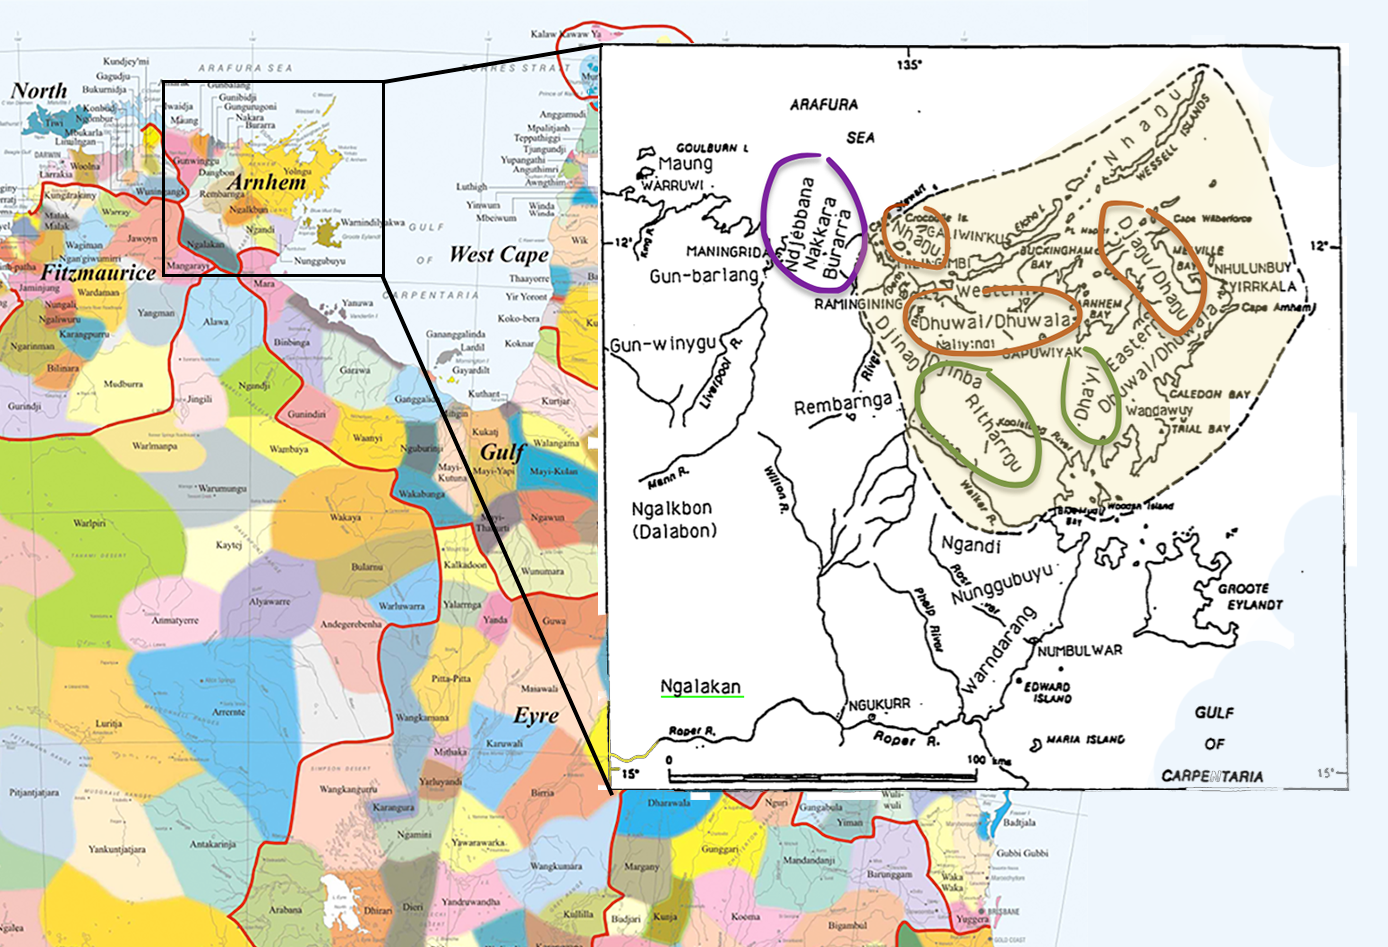
\includegraphics[width=0.7\textwidth]{AustralianLangsCropped.png}\label{map}
\end{figure}




%\section{Dhuwal-Dhuwala: Djambarrpuyŋu \& Gupapuyŋu}\label{djr}

TMA distinctions in Dhuwal(a) are encoded in a paradigm that disinguishes four `inflections', which are cognate with a number proto-Yolŋu inflections according to the reconstructions provided by \citet{Bowern2009}. Work on Dhuwal and Dhuwala varieties (notably \citealt{Wilkinson1991,Lowe1996}) has eschewed a metalinguistic gloss for these inflections, given the ostensible non-unifiability of their semantics. Both authors appeal to an arbitrary numbering system for the four ``inflections'', which I follow in this section. In addition to these inflections, the expressive burden of encoding TMA relations is shared by a (closed) class of auxiliaries, which appear to interact with the verbal paradigm. 

Further complicating the exposition of this, is the fact that there are a number of \textit{conjugation (sub)classes}: 9 according to \citet{Lowe1996} for Gupapuyŋu, 3 larger classes each with a number of subclasses in addition to ``non-inflecting'' and (semi-)irregular categories for the closer description in \citet{Wilkinson1991}.

In this section, I draw predominantly from existing and novel resources on the Djambarrpuyŋu (comprehensively documented by Melanie Wilkinson \citeyearpar{Wilkinson1991}) and Gupapuyŋu (especially with reference to Beulah Lowe's grammar notes and Anita van der Wal's \citeyear{VanderWal1992} doctoralthesis). These two central Arnhem varieties are closely related. Additional references are made to the eastern varieties Djapu \citep{Heath1980b,Morphy1983} and Gumatj. Wilkinson's proposed  phylogeny of Southern Yolŋu is provided (slightly simplified \& modified) as Figure \ref{DDvars} below. See Chapter \ref{ecology} for more background.

\begin{figure}[h]\centering
\begin{tikzpicture}[every node/.append style={align=left},every tree node/.style={anchor=north}]
\Tree [.\textsc{\textbf{Southern~Yolŋu}} [.\textbf{Ritharrŋu} $\vdots$ ] [ [.\textbf{Dhay'yi} $\vdots$ ] [.\textbf{Dhuwal-Dhuwala} [.\textsc{western} \node[text=teal,font=\itshape]{\bf\it Djambarrpuyŋu\\Ḻiyagalawumirr\\Ḻiyagawumirr\\Marraŋu}; \node[font=\itshape,text=ochre]{\bf\it Gupapuyŋu\\Wubulkarra}; ]   [.\textsc{eastern} \node[font=\itshape,text=teal] {Djapu\\Marrakulu\\Ḏäṯiwuy}; \node[font=\itshape,text=ochre]{Gumatj\\Maŋgalili\\Munyuku\\Maḏarrpa}; ] ] ] ]
\end{tikzpicture}
\caption{Varieties (dialects) of \textcolor{teal}{Dhuwal}-\textcolor{ochre}{Dhuwala} in the context of the Southern Yolŋu languages \citep[following][13]{Wilkinson1991}.}\label{DDvars}
\end{figure}

\section{The verbal inflections \& their functional domains}\label{infls}

As mentioned above, Dhuwal(a) varieties make use of a verbal paradigm with four inflectional distinctions. As discussed in Chapter \ref{ecology}, varieties of Dhuwal-Dhuwala are mutually intelligible, the primary distinction resulting from a productive apocope rule (\citealp[51]{Morphy1977}, \citealp[see also][94\textit{ff}]{Wilkinson1991} for further details.). The formal consequences of Dhuwal apocope on the verbal paradigm are shown in Table \ref{djr-pdm-exx} below. The table gives examples of the verb paradigm for each of the major Djambarrpuyŋu conjugation classes as described by \citet[306ff]{Wilkinson1991} (parentheses give the corresponding verb group number assigned by \citet{Lowe1996} for Gupapuyŋu.)

\mcom{Of course I can provide more detailed information (the subclasses) but that feels like it'd be better appended? The comparative spreadsheet i've made/Claire's 2009 stuff has most of this formative data... \\\textbf{note: Andrea Simms strongly suggests more exposition of the formal paradigm} }\begin{table}[h]\centering
	\begin{tabular}{ll|llll}
		\textbf{Class} & \textbf{\textit{Example}} & \textbf{I} & \textbf{II} & \textbf{III} & \textbf{IV}\\\midrule
		$\boldsymbol\emptyset$  (2)& \textit{marrtji} `go' & \textit{marrtji}& \textit{marrtji} & \textit{marrtji\textbf{n(a)}} & \textit{marrtji\textbf{nya}}\\
		
		$\boldsymbol\emptyset_{rr}$  (?)& \textit{waṉḏirr(i)} `run' & \textit{waṉḏi\textbf{rr(i)}}& \textit{waṉḏi} & \textit{waṉḏi\textbf{n(a)}} & \textit{waṉḏi\textbf{nya}}\\
		
		
		
		\textbf{N} (5) & \textit{ḻupthun} `wash' &\textit{ḻuphtu\textbf{n}} & \textit{ḻupthu\textbf{rr(u)}} & \textit{ḻupthu\textbf{rr(una)}} & \textit{ḻupthu\textbf{na}}\\
		 \textbf{Ŋ} (7)  & \textit{nhäma} `see' & \textit{nhä\textbf{ma}} & \textit{nhä\textbf{ŋu}} & \textit{nhä\textbf{ŋal(a)}} & \textit{nhä\textbf{nha}}\\
				\end{tabular}
			\caption{Examples of the paradigm of four morphological TMA inflections in Djambarrpuyŋu [\gls{djr}] and (Gupapuyŋu [\gls{guf}] resyllabification in parentheses).\\{}[\gls{djr}] data from \citet{Wilkinson1991}; [\gls{guf}] data from \textit{Gupapuyŋu} \citeyearpar{Gupapuyngu2016}.} \label{djr-pdm-exx}
\end{table}

In the first paragraph of this section, I alluded to Beulah Lowe's eschewal of a ``semantic description'' for each of the four inflectional classes. Melanie Wilkinson follows this system in her 1991 grammar and I will follow them here. Below I provide examples of the functional domains of each of the four inflections in Dhuwal-Dhuwala. Inflections are glossed with the bold-faced Roman numerals given in Table \ref{djr-pdm-exx}. This section focuses on the interpretation received by inflections in simple sentences (\textit{sc.} matrix clauses) -- complex sentences and predications are investigated in further detail in §\ref{djr-subord}.

Table \ref{Infl-Comparisons-Wilk}, adapted from \citet[336]{Wilkinson1991} summarises the metalanguage decisions made by other authors in their attempts to describe Dhuwal(a) varieties.

\begin{table}[h]
\begin{tabular}{l|llll}
	&	\textbf{I}	& \textbf{II}	&	\textbf{III}	&	\textbf{IV}\\\midrule
\citealt{Wilkinson1991} (Djambarrpuyŋu)&\textsc{First}&\textsc{Second}&\textsc{Third}&\textsc{Fourth}\\
\citealt{Lowe1996} (Gupapuyŋu) &Primary&Secondary&Tertiary&Quartenary\\
\citealt{Tchekhoff1983} (Djambarrpuyŋu)&\textsc{Bas}e&\textsc{Fut}ure&Past\textsubscript1&Past\textsubscript2\\
\citealt{Heath1980} (Dhuwal) & Pres/Fut & Fut/Imp & Past & Past Remote\\
\citealt{Morphy1983} (Djapu) & Unmarked & Potential & Perfective & Past Non-indicative\\
\end{tabular}
\caption{Summary of metalinguistic descriptors for the four inflectional classes in a number of Dhuwal/Dhuwala varities, adapted from \citet[336]{Wilkinson1991}.}\label{Infl-Comparisons-Wilk}
\end{table}

\subsection{The Primary inflection}

The `primary' inflection (\textbf{I}), cognate with inflections in other Yolŋu languages which have been described as ``unmarked'' or ``base'', surfaces in predications about the present, past and future. Here I provide examples of \textbf{I}-inflected clauses receiving each of these temporal interpretations.

\mcom{Now for both of these (and i suspect all sentences in this sssection) context ought to be modulable s.t. a non-present reading is available. This can/should/will be tested in the field}\pex\textit{ Present-reference encoded with \textbf{I}}

\a\begingl\deftagex{IPres}\deftaglabel{nhina}
\gla Ŋunhi-y ŋunhi ḏirramu \textbf{nhina} ga//
\glb \gls{texd}\textsc{-erg} \textsc{texd} man sit.\textbf{I} \textsc{ipfv.\textbf{I}}//
\glft`There that man is sitting.'\trailingcitation{\citep[856]{Tchekhoff1983}}// 
\endgl
%\a\begingl \gla ŋarra \textbf{marrtji}-n dhiyaŋu-n bala//
%\glb 1s go\textbf{.I}-\gls{seq} \gls{prox}.\gls{erg}-\textsc{seq} then//
%\glft`I am going now.'\trailingcitation{\citep[256]{Wilkinson1991}}//\endgl
\a\begingl\gla Ŋarra ga \textbf{ḻuka} gapu (dhiyaŋu bala)//
\glb 1s \textsc{ipfv.\textbf{I}} consume.\textbf{I} water \gls{texd}.\gls{erg} then//
\glft`I'm drinking water at the moment.'\trailingcitation{[DhG 20190405]}//\endgl
\xe

The sentences given in (\getref{IPres}) show the compatibility between present temporal reference and the \textbf{I} inflection: in both cases, the event described by the predicate (\textit{nhina} `sit.\textbf{I}' and \textit{marrtji} `go.\textbf{I}') is understood as being contemporaneous with speech time. Both sentences receive event-in-progress readings (also co-occurring with explicit aspectual marking, see §\ref{djr-asp} for more.)

\mcom{Is it a shitty idea to use colour coding for more formatting/highlighting options? I want to resolve bold for the verbforms themselves but would like to be able to second-order emphasise non-paradigmatic things like TFAs, aspectual ops...}
\pex \textit{Past-reference encoded with \textbf{I}}\deftagex{pstI}

%\a\deftaglabel{nhama}\begingl\gla barpuru linyu \textbf{nhäma} dirramu-ny//
%\glb yesterday 2d see.\textbf{I} boy-\gls{acc}//
%\glft`Yesterday we saw a boy'\trailingcitation{\citep[569]{Tchekhoff1985}}//\endgl


\a\deftaglabel{ŋayatham}\begingl\gla ga \textbf{ŋayatham} ŋunha baṉ'thula-wuy ŋayambalk//
\glb and reach.\textbf{I} \gls{dist} \textsc{place}-\gls{assoc} place//
\glft`And (then we) reached the place (associated with) Baṉthula.'\trailingcitation{\citep[461]{Wilkinson1991}}//\endgl



\a\deftaglabel{rrupiya}\begingl\gla ḏirramu-wal yothu-wal bäpa-'mirriŋu-y rrupiya barpuru djuy'yu-\textbf{n} märr barpuru ga barpuru \textbf{buna}-ny dhiyal-nydja//
\glb man-\gls{obl} kid-\gls{obl} father-\gls{kinprop}-\textsc{erg} money yesterday send.\textbf{I} somewhat yesterday and yesterday arrive.\textbf{I}-\textsc{prom} \gls{prox}.\gls{erg}-\gls{prom}//
\glft`The father sent money to the boy recently and it arrived here yesterday'\trailingcitation{\citep[343]{Wilkinson1991}}//\endgl

\xe

Additionally, the sentences given in (\getfullref{pstI}) show compatibility between \textbf{I} and past time reference. For both examples the events described by the predicates (e.g. the seeing event described by \textit{nhäma} in (\getref{pstI.ŋayatham})) \textit{precede} speech time. Similarly, the two past events in (\getref{pstI.rrupiya}) both receive \textbf{I} inflection. The instantiation times of both of these events are restricted by with \textit{barpuru} $\approx$ `yesterday. -- frame adverbials of this type are discussed in some detail in §\ref{TFA}.

\pex \deftagex{futI} \textit{Future-reference encoded with \textbf{I}}
\a\deftaglabel{lakaram}\begingl\gla yalala ŋarra dhu nhokal lakara-\textbf{m}//
\glb later 1s \textsc{fut} 2s\textsc{.obl} tell-\textbf{I}//
\glft `Later (today) I'll tell you.' \trailingcitation{\citep[373]{Wilkinson1991}}//\endgl

\a\deftaglabel{buna}\begingl \gla dhiyaŋ~bala walal dhu \textbf{buna}, yalala//
\glb now 3p \textsc{fut} arrive.\textbf{I} later//
\glft`They are coming later today.'\trailingcitation{\citep[256]{Wilkinson1991}}//\endgl


\a\begingl\glpreamble Deontic force with \textit{dhu}+\textbf{I} (see §\ref{dhu})//
\gla Way! Nhe dhu gurruka-\textbf{m} helmet! Rom ga \textbf{waŋa}.//
\glb Hey! 2s \gls{fut} wear-\textbf{I} \textit{helmet} law \textsc{ipfv.\textbf{I}}  say.\textbf{I}//
\glft`Oy! You wear a helmet! The law says so!\trailingcitation{[AW~20170730]}//\endgl

\a\deftaglabel{marrtji}\mcom{Actually, W claims this is ``imminent action'' so we really just have a futurate use of \textbf{I} without \textit{dhu} (interesting data point in itself) This can probably move to the section on future marking (either \textbf{I} or \textbf{\textit{dhu}})}\begingl\glpreamble `Imminent action' without \textit{dhu}//
\gla \ljudge{$ ^{\%*} $}ŋarra marrtji-n \textbf{dhiyaŋu}-n \textbf{bala}//
\glb 1s go-\gls{seq} \textbf{\gls{prox}.\gls{erg}}-\gls{seq} \textbf{\gls{mvtawy}}//
\glft`I'm going now.'\trailingcitation{\citep[256]{Wilkinson1991}}//\endgl

\xe


Finally, the examples in (\getref{futI}) above, show the compatibility of \textbf{I}-inflected verb forms and future temporal reference. In both sentences, the event described by the predicate is understood to obtain in the \underline{future} of speech time (modulo additional constraints on imminence/immediacy described below). \mcom{Evidence of infelicity of \textit{dhu}-less future readings? I actually kinda doubt on the basis of Tonnhauser, Bohnemeyer's work that this is going to be a hard constraint} In these sentences the presence of \textsc{fut} marker \textit{dhu} is apparently obligatory in order to establish future reference. (Although according to \citet[256]{Wilkinson1991} (\getfullref{futI.marrtji}), a futurate interpretation is ostensibly available. This use is unavailable to Ramingining speakers.

\subsection{The Secondary inflection}

Like \textbf{I}, the Secondary inflection (\textbf{II}) has a range of uses. It is notably obligatory when predicating of future times \underline{beyond the current day} and is the main strategy for forming \underline{imperative sentences}.

\pex\deftagex{futII} \textit{Future-reference encoded with \textbf{II}}
\a\deftaglabel{lakaraŋ}\begingl\glpreamble Co-occurring with \textit{dhu} `\gls{fut}'//
\gla yalala-ŋu-mirri-y ŋula~nhätha ŋarra dhu nhokal lakara\textbf{-ŋ}//
\glb later-\textit{ŋu}-\gls{prop}-\gls{erg} sometime 1s \textsc{fut} 2s-\gls{obl} tell-\textbf{II}//
\glft`I'll tell you sometime later on'\trailingcitation{\citep[346]{Wilkinson1991}}//
\endgl
\a\deftaglabel{nhini}\begingl\glpreamble Future interpretation independent of \textit{dhu} `\gls{fut}'//
\gla ŋayi boŋguŋ \textbf{nhini} \textbf{ŋäku} ŋarra-ny ŋunhal yirrkala//
\glb 3s tomorrow sit.\textbf{II} hear.\textbf{II} 1s-\gls{prom} \gls{dist}-\gls{loc} \textsc{placename}//
\glft`She'll be there at Yirrkala tomorrow, listening to me'\trailingcitation{\citep[340]{Wilkinson1991}}//\endgl

\a\begingl\glpreamble Infelicity of \textbf{I} with non-today future//
\gla Barpuru goḏarr ŋarra dhu nhä(\textbf{-ŋu/$^*$-ma})//
\glb funeral tomorrow 1s \gls{fut} see(-\textbf{II}/$^*$-\textbf{I})//
\glft `I'll see the funeral tomorrow'\trailingcitation{[AW~20180730]}//\endgl

\xe

The two sentences in (\getref{futII}) show how \textbf{II} is used to establish future temporal reference. The conditions on the (non-)appearance of \textsc{fut}-marker \textit{dhu} are unclear at the present time (see §\ref{dhu} for more), but future-readings with \textbf{II} do not appear to be reliant on this auxiliary (cf. the data in (\getref{futI}) above). A notable contrast between (\getfullref{futI.lakaram}) and (\getfullref{futII.lakaraŋ}) is the apparently obligatory retrieval of a \textsc{today}-reference time for \textbf{I}-inflected futures, as against a (probable) \textsc{beyond-today}-reference time for \textbf{II}-inflected futures.\footnote{\citet[347]{Wilkinson1991} gives an example of a speaker using a \textit{dhu}-\textbf{II} structure in the context of a narrative she is telling, signalling that she `will (return to the time of the old people).' Wilkinson takes this as evidence of an association between \textbf{II} and the irrealis. This generalisation is pursued in detail in the next chapter of this dissertation.} Effectively, this distinction seems to be one place where the grammar of Dhuwal(a) grammaticalises ``temporal remoteness'' (\citet{Comrie1985,Dahl1985} referred to elsewhere in the literature as `metrical tense' \citealp[e.g.][204]{Chung}).\footnote{Although \citet[39]{Heath1980} suggests of the \textbf{II} future in Dhuwal Proper (his \textsc{Fut/Imp}) that this form encodes a type of ``normative nuance'' (a clear extention of imperative flavour into future assertions.)}


\mcom{It would be good to get sentences with richer context (i.e. an established time of instantiation for the prejacent (tomorrow, imminently etc...)) This said we can probably assume that the we're talking about immediate future here... Is \textbf{I} incompatible with this? There's not much more to say here until I have speaker judgments on this question.}\pex\deftagex{irrII}\begingl\gla Ŋarra ŋuli bäynha \textbf{dhiŋgun} ŋawulul-yu//
\glb 1s \textsc{hyp?} \textsc{mod?} die.\textbf{II?} smoke-\textsc{erg?}//
\glft`I might die from the smoke.'\trailingcitation{\citep[164]{Buchanan1978}}//\endgl\xe


(\getref{irrII}) shows the compatibility of \textbf{II} with a future-oriented possibility reading. The modal particles \textit{ŋuli} and \textit{bäynha} are responsible for the `weakening' or `downtowning' of the speaker's commitment to the prejacent proposition. Modal operators are described in §\ref{modals}.


\pex\textit{Imperative force with \textbf{II}}\deftagex{impII}
%\a\begingl\gla g...y, ḻupmara-\textbf{ŋu}-n ŋarra-ny//
%\glb \textsc{name} wash-\textbf{II}-\gls{seq} 1s-\gls{prom}//
%\glft`G...y, wash me!'\trailingcitation{\citep[360]{Wilkinson1991}}//\endgl

\a\begingl\gla wäy! gurtha ŋunha, nhawi, ḏutji män-\textbf{ŋu}, bakmara-\textbf{ŋu}//
\glb hey! fire(wood) \gls{dist} what's.it firesticks get-\textbf{II} break\textbf{-II}//
\glft`Hey! Get that firewood, what's it, those firesticks, and break them.'\trailingcitation{\cite[114]{VanderWal1992}}//\endgl




\a\deftaglabel{proh}\begingl\gla yaka walala-ŋ buku-bakamara-\textbf{ŋ}//
\glb \gls{neg} 3p-\gls{dat} head-break-\textbf{II}//
\glft `Don't answer them!'\trailingcitation{\citep[360]{Wilkinson1991}}//\endgl


\a\begingl\gla nhä\textbf{-ŋu} nhanŋu dhurrwara!//
\glb look-\textbf{II} 2s.\gls{dat} door//
\glft`Look at her mouth!'\trailingcitation[AW 20180731]//\endgl

\xe


The sentences in (\getref{impII}) show the imperative function of \textbf{II}-inflected clauses. Shown in (\getfullref{impII.proh}), negative imperatives (probibitives) are treated identically.\footnote{Although the use of privative-marked nominals is another common strategy, se.e \citet{Phillips2018a,Phillips2019} for more.}

\subsection{The Tertiary inflection}

The Tertiary inflection (\textbf{III}) is generally associated with predications about the \textsc{past}. An important caveat, however, is that this inflection is \ul{infelicitous when describing \textsc{recent} events instantiated \textsc{before the current day}.} The examples in (\nextx) below show the compatibility between \textbf{III} and a reference time that is `earlier today.'\mcom{Show the compatibility of \textbf{III} with \gls{ipfv} by adding some examples with \textit{gana}. (Perhaps a minimal pair, though this might be better placed below.)}

\pex \textit{\textsc{Today past} and the \textbf{III} inflection}\deftagex{pstIII}
\a\deftaglabel{gathur}\begingl\gla Gäthur ŋayi \textbf{marrtjin} räli Galiwin'ku-ŋur//
\glb today 3s go.\textbf{III} hither \textsc{place}-\gls{abl}//
\glft`[Earlier] today he came from Galiwin'ku.'\trailingcitation{\citep[150]{Buchanan1978}}//\endgl

\a\deftaglabel{bili}\begingl\gla Bili ŋayi \textbf{marrtjin} dhipuŋur natha-ŋur nyan'thuna-ŋur//
\glb \textsc{compl} 3s go.\textbf{III} \textsc{prox.abl} food-\gls{abl} eat.\textbf{IV}-\textsc{abl}//
\glft`He has already gone from having lunch here.'\trailingcitation{\citep[150]{Buchanan1978}}//\endgl


\a\begingl\glpreamble Infelicity of \textbf{III} with \textsc{recent past}//
\gla barpuru ŋarra nhä\textbf{(-ma/*-ŋala)} ḏetuŋ//
\glb yesterday 1s see\textbf{(-I/$^\#$-III)} buffalo//
\glft`I saw a buffalo yesterday.'\trailingcitation[MD 20180802]//\endgl

\a\begingl\glpreamble Infelctity of \textbf{I} with \textsc{today past}//
\gla gathura ŋarra nhä\textbf{($^\#$-ma/-ŋala)} ḏetuŋ dhukarra-ŋura//
\glb today 1s see\textbf{$ ^\# $-I/III} buffalo road-\gls{loc}//
\glft `I saw a buffalo today'\trailingcitation{[MD 20180802]}\\\textsc{comment.} Event could have happened this morning or ten minutes before speech time.//\endgl
\xe

\mcom{Potentially look for a ref for this or provide data that makes this unambiguous...}(\getfullref{pstIII.gathur}) shows the compatibility between temporal frame adverbial (TFA) \textit{gäthur(a)} `today' and \textbf{III} in \gls{djr}, which leads to an temporal interpretation of `earlier today.'\footnote{Note however that the reckoning of \gls{tfa} \textit{gäthur(a)} differs to that of English and other familiar languages as shown in (\getfullref{neg-pst.munha}), where \textit{gäthur munhawa} `today nighttime' is interpreted as ``last night'' and still triggers \textbf{III} marking on the verb.} However even in the absence of a \gls{TFA}, the event described in (\getref{pstIII.bili}) is interpreted as having been instantiated \textsc{earlier.today}/in the immediate past of speech time. \textbf{III} cannot, however, be conveniently described as a `hodiernal past' (cf. Mwera?, also \citealt[86]{Comrie1985}), as the data in (\nextx) make clear.


\pex\textit{\textsc{Remote past} and the \textbf{III} inflection}\deftagex{remIII}

\a\deftaglabel{wawa}\begingl\gla nhä nho-kiyin-gal wäwa-'mirriŋu-y warkthu-rr ŋäthil rarrandharr-yu//
\glb what 2s-\textsc{emph}-\gls{obl} bro-\gls{kinprop}-\gls{erg} work-\textbf{III} before dry~season-\gls{erg}//
\glft`What did your brother do last summer?'\trailingcitation{\citep[343]{Wilkinson1991}}//\endgl

\a\deftaglabel{malwan}\begingl\glpreamble\textsc{context.} The speaker is describing a locality as it was in her youth.//
\gla märrma' ga-\textbf{n} malwan-dja dhärra-\textbf{n} yindi maṉḍa-ny//
\glb two \textsc{ipfv}-\textbf{III} hibiscus-\gls{prom} stand-\textbf{III} big 3d-\gls{prom}//
\glft`Two big hibiscus flowers were (growing).'\trailingcitation{\citep[339]{Wilkinson1991}}//\endgl

\a\deftaglabel{wuŋgan}\begingl\glpreamble\textsc{context.} A man is telling a story from long ago . His friend's dog has spotted a water goanna.//
\gla ...ŋunhi wurkaḏi-y nhä-ŋal-{na} ŋinya dharpa-lil-a ŋal'yu-na nhäwi wan'kawu-ya//
\glb \gls{texd} \textsc{name}-\gls{erg} see-\textbf{III} 3s.\gls{acc} tree-\gls{all}-\gls{seq} ascend-\textbf{III} whatsit water.goanna-\gls{ana}//
\glft`\textit{Wukaḏi} watched it scramble up into a tree, the water goanna.'\trailingcitation{\citep[193]{Heath1980b}}//\endgl\mcom{I've taken some liberties with the glossing here, Heath has the second verb \textit{ŋal'yuna} as \textbf{I} with a \textsc{seq} marker... to investigate further perhaps}



\xe


Unlike the \textsc{hodiernal} temporal interpretations that the sentences in (\blastx) receive, the two sentences in (\lastx) are evaluated to obtain in the `\textsc{remote past}.' In (\getfullref{remIII.wawa}),\mcom{may be easier just to get a similar non-interrogative sentence to do what \lastx b does} the instantiation time of the predicate is restricted by two frame adverbials: \textit{ŋäthil(i)}, which picks out a time `in the distant past; prior to/earlier than (some other predicate)' \citep[158]{Wilkinson1991} and \textit{rarrandharryu} `dry season':\footnote{The suffix \textit{-Thu} (\textit{-yu} as a postsonorant allomorph), glossed here as \gls{erg} is used to mark ergative NPs as well as instrumental (\gls{instr}) NPs and to form TFAs out of nominals \gls{temp}.} The cooccurrence of these expressions restricts the predicate being questioned to \textit{a prior dry season}. Conversely, the declarative sentence in (\getfullref{remIII.malwan}) requires no adverbial specification. A \textsc{remote past} interpretation arises as a result of the \textbf{III} inflection alone, which is precised pragmatically by the discourse context (\textit{sc.} a narrative that the speaker is telling about her childhood.)\mcom{Provide some negative felicity judgments} In principle, \getfullref{remIII.malwan} ought to be able to retrieve a same-day past interpretation as well, with sufficient contextual support.

\mcom{This discussion of the Maningrida treatments of `frame' and `tense' may be better placed • entirely in the lit. review, • after the general data discussion of inflections, or • in the following chapter.} The ostensible `discontinuity' of the times predicates receiving \textbf{I} and \textbf{III} inflection can refer to has been described in preceding literature as \textbf{\textsc{cyclic time reference}} \citep[88]{Comrie1983}. In her influential treatment of Burarra [\gls{bvr}], \citet{Glasgow1964} draws a distinction between `tense' and `frame of reference' (`timescale' for \citealt[48]{Green1987}). The interaction between these is taken to give rise to a reference interval. This analysis has been adopted and developed by others working on Maningrida languages (\citet[165]{Eather2011} for Nakkara [\gls{nck}], \citet{Green1995} for Gurr-goni [\gls{gge}] and \citet{McKay2000}.) This is schematised in Table \ref{GlaswegianTR}. The following chapter further treats and formalises this analysis.


% Please add the following required packages to your document preamble:
% \usepackage{booktabs}
% \usepackage{multirow}
\begin{table}[h]\centering\onehalfspacing
	\begin{tabular}{@{}llll@{}}\toprule

		&                 & \multicolumn{2}{c}{\textsc{frame}}          \\ 
		&                 & \multicolumn{1}{c}{\textbf{today}}         & \multicolumn{1}{c}{\textbf{before today}}      \\\midrule
		\multirow{2}{*}{\textsc{\rotatebox[origin=c]{90}{infl}}} & \textbf{\phantom{I}I}    & now           & yesterday/recently \\
		& \textbf{III} & earlier today & long ago           \\ \bottomrule%(l){2-4} 
	\end{tabular}
\caption{A \citet{Glasgow1964}-style analysis of \textbf{past-time restrictions} introduced by the verbal inflections, adapted for the Dhuwal(a) data. \textbf{I} and \textbf{III} inflections correspond to Eather's \textbf{contemporary} and \textbf{precontemporary} ``tenses'' (``precontemporary'' is Eather's \citeyearpar[166]{Eather2011} relabelling of Glasgow's ``remote'' tense.)}\label{GlaswegianTR}
\end{table}
\mcom{Also the get sick/psych/phys condition verbs, some examples also in Buchanan:168}


Additionally, a set of psychological predicates that are frequently translated into English as present-tensed stative verbs appear with \textbf{III}. Examples are given in (\nextx).


\pex\deftagex{psychPreds}\a\begingl\gla ŋarra dhuwal/dhika djawaryu-\textbf{rr}/rerrikthu-\textbf{rr}/djanŋarrthi-\textbf{n}//
\glb 1s \textsc{prox/indefp} be.tired-\textbf{III}/be.sick-\textbf{III}/be.hungry-\textbf{III}//
\glft`I'm (a bit) tired/sick/hungry'\trailingcitation{\citep[278]{Wilkinson1991}}//\endgl
\a\begingl\gla bili djawar'yu-\textbf{rr}-a//
\glb \gls{cplv} be.tired-\textbf{III}//
\glft`They're already tired'\trailingcitation{\citep[365]{Wilkinson1991}}//\endgl
\mcom{Needs elicitation work, appears to be a today-past thing? Are these predicates available with TFAs \textit{barpuru?}, with \textit{ga}? And the other inflections??\\
Test entailments also: \textit{??I was tired this morning but i'm not now??}}
\a\deftaglabel{nhaŋal}\begingl\gla ŋarra dhu dhuwal lakara-m ƞunhi nhä ŋarra nhä-\textbf{ŋal} dhiyaŋ bala//
\glb 1s \gls{fut} \gls{prox} tell-\textbf{I} \gls{texd} what 1s see-\textbf{III} \gls{prox}.\gls{erg} \gls{mvtawy}//
\glft`I'll tell you what I see right now.'\trailingcitation{\citep{Wilkinson1991}}//\endgl
\xe

\citet[365-6]{Wilkinson1991}, in effect, suggests that the frequent exponence of \textbf{III} in these predicates of ``emotional and bodily states'' is a function of their lexical semantics. Unlike their English translations, with \textbf{III}, these predicates can be understood as `achievements' (to borrow from Vendler's Aktionsart taxonomy). In these cases then, \textbf{III} is licensed because \textit{djarwaryu\textbf{rr(u)}} refers to a state-change before speech time. Consequently, the licensing of \textbf{III} in (\getfullref{psychPreds.nhaŋal}) above is a consequence of a completed \textit{seeing} eventuality immediately prior to the \textit{telling}-event described in the matrix clause. This phenomenon is investigated in detail in §\ref{anY}\texttt{.1?} below.


\subsection{The Quaternary inflection}


\mcom{Is this XLinguistic note worth anything? If so a couple more examples would be nice.}The Quartenary inflection (\textbf{IV}) has a broad range of uses in Dhuwal(a) varieties that correspond in part to categories described in Australian languages including \textit{past potentialis} \citep{Heath1980a}, \textit{past counterfactual} \cite{McKay2011}, \textit{[past] irrealis} \citep[159]{Austin1998} \textit{etc.} It is used primarily with modal auxiliaries in order to describe past habituals (\getref{habIV}) with \textit{ŋuli} and past irrealis event description (with \textit{balaŋ} a.o.) as in (\getref{hypIV}) including counterfactuals.


\pex\a\deftagex{habIV}\begingl\gla Ŋayi ŋuli märra-\textbf{nha} ŋunhi meṉḏuŋ-nha//
\glb 3s \gls{hab} get-\textbf{IV} \gls{texd} snail-\gls{acc}//
\glft`She would (used to) get (collect) snails'\trailingcitation{\citep[147]{Buchanan1978}}//\endgl

\mcom{check ft for (b)}\a\begingl\gla ...ŋorra-\textbf{nha} walal ŋuli marrtji-\textbf{nya} ŋunhi-li-yi, galku-\textbf{na} walal ŋuli ga-\textbf{nha} gapuw wirwiryu-\textbf{na}+ra-w//
\glb lie-\textbf{IV} 3p \textsc{hab} go-\textbf{IV} \textsc{texd}-\gls{loc}-\gls{ana} wait-\textbf{IV} 3p \textsc{hab} \textsc{ipfv}-\textbf{IV} water-\gls{dat} turn-\gls{nmlzr}-\gls{dat}//
\glft`They would be lying there, they would be waiting for the water to stir.'\trailingcitation{(DB Djon 5:4)}//\endgl

\xe


\pex\a\begingl\glpreamble\deftagex{hypIV}\textsc{context.} Speaker had a toothache.//
\gla barpuru balaŋ ŋarra bala dentist-kal marrtji-\textbf{nya} dhiyak//
\glb yesterday \textsc{irr} 1s \gls{mvtawy} dentist-\gls{obl} go-\textbf{IV} \gls{prox}-\gls{dat}//
\glft`Yesterday I should have gone to the dentist for a filling'\trailingcitation{\citep[353]{Wilkinson1991}}//\endgl

\a\begingl\gla Yaka balaŋ nhe marrtji-\textbf{nya} Darwin-lil//
\glb \gls{neg} \textsc{irr} 2s go.\textbf{IV} Darwin-\gls{all}//
\glft`You should not go to Darwin.'\trailingcitation{\citep[164]{Buchanan1978}}//\endgl\xe


These data demonstrate the relationship between the \textbf{IV} inflection and combinations of past temporal reference and various modal and aspectual operators. These categories are treated in more detail in §\ref{modals} below. Furthermore, the data presented so for in this section are predominantly positive sentences. §\ref{negs} describes striking interactions between negation operators and verbal inflectional categories in some Dhuwal(a) varieties.

\section{Sentential negation: \textit{yaka} \& \textit{bäyŋu}}\label{negs}

Djambarrpuyŋu has two negative particles, \textit{yaka} and \textit{bäyŋu}, which are deployed for standard negation (i.e. those particles whose effect is to reverse the truth value of a given proposition.) The particles differ in that only \textit{yaka} is used to generate negative imperatives (prohibitives) and only \textit{bäyŋu} is found in negative existential/quantificational contexts (see \citet{Phillips2019b} for further discussion of semantic change in the Yolŋu negative domain.) Remarkable, however, is the complex interaction between sentential negation and verbal inflection.

Descriptively, negation appears to trigger a ``switch'' from the `realis-aligned inflections' (\textbf{I}~and~\textbf{III}) to their `irrealis counterparts' (\textbf{II}~and~\textbf{IV}), effectively evincing a mood-based distinction that is neutralised in negated sentences \citep[following ][356]{Wilkinson1991}. This is schematised below in Table \ref{negneut}.

\begin{table}[h]\centering
	\begin{tabular}{ccc}
		&\multicolumn{2}{c}{\textsc{\textbf{polarity}}} \\
		& \textsc{--neg} & \textsc{+neg}\\\midrule
	&	\textbf{I} & \multirow{2}{*}{\textbf{II}}\\
	& \textbf{II} \\\midrule
	&	\textbf{III} & \multirow{2}{*}{\textbf{IV}}\\
	& \textbf{IV} \\\bottomrule
	\end{tabular}
\caption{Neutralisation of \textbf{I} and \textbf{III} inflections under negation.}\label{negneut}
\end{table}


\pex\textit{Present/recent.past \textbf{I} expones as \textbf{II} under negation}\label{neg-pres}


\a\begingl\glpreamble  Negated present-tense sentence receives \textbf{II} marking\\\textsc{context.} Speaker is trying to read from a computer screen.//
\gla bäyŋu ŋarra \textbf{gi} nhä-\textbf{ŋu}//
\glb \gls{negq} 1s \gls{ipfv}.\textbf{II} see-\textbf{II}//
\glft`I can't see (it).'\trailingcitation{[AW 2018030]}\\\textsc{comment.} \textit{nhäŋu} (`see.\textbf{II}') could also mean yesterday, in past.//\endgl

\a\begingl%\glpreamble Negated present-tense sentence receives \textbf{II} marking//
\gla yaka \textbf{gi} \textbf{biyak} rom waŋ-\textbf{i}//
\glb \gls{neg} \gls{ipfv}.\textbf{II} do.thusly.\textbf{II} law say-\textbf{II}//
\glft`That's not how the law is/what the law says.'\trailingcitation{\citep[357]{Wilkinson1991}}//\endgl


\a\begingl\glpreamble Present-tensed sentence with \textbf{I}//
\gla Nhaltja-\textbf{n} \textbf{ga} limurru-ŋgu-ny rom waŋ-\textbf{a}?//
\glb do.how-\textbf{I} \gls{ipfv}.\textbf{I} 1p.\gls{incl}-\gls{dat}-\gls{prom} law say-\textbf{I}//
\glft`What does our law say?'\trailingcitation{(DB~Luk~14.3)}//\endgl


\a\begingl\glpreamble Negated (recent) past-tensed sentence receives \textbf{II} marking.\\
\textsc{context.} A recent hunting trip, narrated in \textbf{I} for corresponding positive descriptions.//
\gla ga yaka ŋayi ŋunhi dharyu-rr biyak djin'tjiŋdhu-rr//
\glb and \gls{neg} 3s \gls{texd} rain-\textbf{II} do.thusly.\textbf{II} rain~lightly.\textbf{II}//
\glft`...and it did not rain lightly'\trailingcitation{\citep[357]{Wilkinson1991}}//
\endgl

\xe


\pex Past-tensed sentences exponing with \textbf{IV} under negation\deftagex{neg-pst}
\a\deftaglabel{munha}\begingl\gla bäyŋu ŋarra gäthur ŋorra-\textbf{nha} manymak-ku-\textbf{nha} munhawu//
\glb \gls{negq} 1s today lie-\textbf{IV} good-\gls{tr}-\textbf{IV} nighttime//
\glft`I didn't sleep well last ni	ght'\trailingcitation{\citep[357]{Wilkinson1991}}//\endgl

%\mcom{Though the second clause in (b) also has ŋuli so maybe this is not quite so nice an ex. as originally thought}\a\begingl\gla ŋäthil-nydja ŋarra ga-n dhuwal, ga miltjiri marrtji-n \ bäyŋu ŋarra ŋuli ga-\textbf{nha} nhä-\textbf{nha}//
%\glb earlier-\gls{prom} 1s \gls{ipfv}-\textbf{III} \gls{prox} and blind go-\textbf{III} \textbackslash \gls{negq} 1s \gls{hab} \gls{ipfv} see-\textbf{IV}//
%\glft`I was blind before; I was unable to see'\trailingcitation{\citep[358]{Wilkinson1991}}//\endgl


\a\begingl\gla gathur munhagumirr ŋarra nhä-\textbf{ŋal} warrakan//
\glb today morning 1s see-\textbf{III} bird//
\glft`I saw a bird this morning'\trailingcitation{[FW 20180802]}//\endgl


\a\begingl\gla gathur munhagumirr bäyŋu ŋarra nhä-\textbf{nha} warrakan//
\glb today morning \gls{neg} 1s see-\textbf{III} bird//
\glft`I didn't see a bird this morning'\trailingcitation{[FW 20180802]}//\endgl

\a\begingl\glpreamble \textsc{context.} Speaker has dropped a coin.//
\gla Way! Bäyŋu ŋarra nhä-nha?//
\glb Hey! \gls{negq} 1s see-\textbf{IV}//
\glft`Ah! Did you see (it)?'\trailingcitation{[AW 20180830]}//\endgl

\a\begingl\glpreamble Negated (distant) past receives \textbf{IV} marking.\\
\textsc{context.} The text describes remote past events, narrated in \textbf{III} for corresponding positive descriptions//
\gla ŋayi-ny muka bäyŋu yan yolŋu-ny yurrumdhu-\textbf{na}//
\glb 3s-\gls{prom} okay \gls{negq} \gls{emph}  person-\gls{prom} gather-\textbf{IV}//
\glft`Not all the people had gathered together'\trailingcitation{\citep[357]{Wilkinson1991}}//\endgl


\xe

\mcom{It's not clear how I can easily get a the status of this alternation via elicitation (esp. if its intraspeaker..?) or whether I should just abstract away from it. My informants so far seem to have consistently respected this alternation.}Notwithstanding this generalisation, \citet[358\textit{ff}]{Wilkinson1991} notes that there exists a considerable amount of synchronic variation in the formal (neutralising) relation between negation and inflection. \Citet[110]{VanderWal1992} in fact reports no asymmetry in her study of Gupapuyŋu, noting that it is just as valid to predict the affirmation of a proposition with future temporal reference as it is to predict the negation of such a proposition.' (\nextx) gives examples of `unexpected' realis-aligned inflections appearing under negation.

\pex Exponence of \textbf{I} and \textbf{III} under negation.


\a\begingl\gla ga yaka-na ŋarra yurru bulu roŋiyi-\textbf{rri}//
\glb and \gls{neg}-\gls{prom} 1s \gls{mod} again return-\textbf{I}//
\glft`And I will not come back again.'\trailingcitation{\citep[110]{VanderWal1992}}//
\endgl


\a\begingl \gla bäyŋu ŋayi ga dhuwal nhina dhiyaŋu-ny bala//
\glb \gls{negq} 3s \gls{ipfv}.\textbf{I} \gls{prox} sit.\textbf{I} \gls{prox}.\gls{dat}-\gls{prom} \gls{mvtawy}//
\glft`She isn't living here now'\trailingcitation{\citep[358]{Wilkinson1991}}//\endgl
\mcom{I suspect a good way of excluding this data will be to test its acceptability with my consultants. I expect Albert, Faith will reject all of these.\\If so is this whole discussion something that should be in fn or Ch.\ref{diaY} rather than in body here?}
\a\begingl \gla gurrupa-\textbf{r} muka ŋarra ga-\textbf{n}, yurr bäyŋu-n ŋayi ga-\textbf{n} ḻuka-\textbf{n}, ŋatha-ny//
\glb give-\textbf{III} \textsc{ok} 1s \gls{ipfv}-\textbf{III} but \gls{negq} 3s \gls{ipfv}-\textbf{III} eat-\textbf{III} food-\gls{prom}//
\glft`I was giving (him) the food but he wasn't eating it'\trailingcitation{\citep[358]{Wilkinson1991}}//\endgl

\xe

Generally, there seems to be a perception (Melanie Wilkinson \textit{pers. comm.}, independently supported by consultant AW [20180830]) that the maintenance of \textbf{I} and \textbf{III} (the `\textsc{realis}-aligned' inflections) under negation is a characteristic of \textit{Miwatj} varieties of Dhuwal-Dhuwala (i.e. those spoken in towards the East.) This is suggestive of an areal/contact phenomenon, a siutation to be further discussed in Chapter \ref{diaY}.

\mcom{There's a great comment from my consultant in her translation of a negative sentence. When asked why \textbf{\textit{gi+}II} was used instead of \textbf{\textit{ga+}I} she claims `not happening yet' (20180802-8min)}\citet[356]{Wilkinson1991} notes that ``[she has] not been able to determine a functional basis for this alternation.'' Nevertheless, in his typological survey of standard negation, \citet[558]{Miestamo2005} identifies a cross-linguistically attested mood-based asymmetry where negative marking triggers the appearance of the irrealis or other ``nonrealised''-type modal markings. This phenomenon seems to be particularly well-represented in the languages of the Top End, functional explanations generally emphasising the fact that negated predicates `[belong] to the realm of the non-realized', a domain associated with irrealis marking (\citealt[225]{Miestamo2005}, cf. \citealt[195]{McLellan1992}, \citealp[see also][]{Phillips2019}). These ideas are explored in further detail in Chapter \ref{anY} below.

\citet{Wilkinson1991} also suggests that there is insufficient cross-linguistic data to assess a the diachrony (and potential areal diffusion) of this asymmetry (356), although provides a concise review of other authors' observations of Yolŋu varieties (359-60). Data about the interactions between polarity and verbal inflection are provided in the following sections and the question of the development of these asymmetries is treated in Chapter \ref{diaY} below.


\section{\textit{dhu}}\label{dhu}

\textit{dhu} (and apparent synonym/dialectal variant \textit{yurru}) is treated as a \gls{fut}-particle by \citet[346]{Wilkinson1991}, Lowe and \citet[39,46]{Heath1980b}. Also available are deontic and epistemic modal readings (such that \citet[110]{VanderWal1992} glosses this particle as \gls{mod}.) These uses of \textit{dhu} are shown in (\getref{dhuT}-\getref{dhuM}) below.

\pex\deftagex{dhuT}\begingl\glpreamble Future reading of \textit{\textbf{dhu}}//
\gla yaka-na \textbf{dhu} limurru roŋiyi-\textbf{rri} Yirrkala-lili//
\glb \textsc{neg-foc} \textsc{\textbf{mod}} 1p\textsc{.inc} return-\textbf{I} Yirrkala\textsc{-all}//
\glft`We won't return to Yirrkala'\trailingcitation{\Citep[125]{VanderWal1992}}//\endgl\xe



\pex\deftagex{dhuM}\textit{Modal readings of \textbf{dhu}}




\a\begingl\glpreamble\textit{Deontic necessity reading of \textbf{dhu}}\\\textsc{context.} Speaker's 16 year-old \textit{waku} has just got his driver's license.//
\gla gaŋga nhe \textbf{dhu} ga gäma mutika-y//
\glb slowly 2s \textbf{\gls{fut}} \gls{ipfv} carry.\textbf{I} car-\gls{erg}//
\glft `You should/must drive slowly.'\trailingcitation{[FW?~20180802]}//\endgl
\mcom{elicit ''you should but you don't have to''\\A future deontic presumbaly takes \textbf{\textit{dhu}+II}}


\a\mcom{The ambiguity between circ nec and fut readings here is super interesting because it really throws the polysemy of \textit{bala} into relief as picking up either $ t* $ or $ w* $}\begingl\glpreamble \textit{Circumstantial necessity reading of \textbf{dhu}}\\\textsc{context.} Child drank a lot of water before boarding a now mid-flight aeroplane.//
\gla Bäpa, gupa ŋarra dhu (bala) waryu-n!//
\glb \textsc{Fa} water 1s \gls{fut} (\gls{mvtawy}) urinate-\textbf{I}//
\glft`Dad, I need to wee now!'\trailingcitation{[AW 20180830}//\endgl

\a\begingl\glpreamble \textit{Deontic impossibility reading of \textsc{neg+}\textbf{dhu}}//
\gla ga yaka-dhi walala \textbf{dhu} \textbf{ga} yatjun-\textbf{dhi}//
\glb and \textsc{neg-ana} 3p \textsc{\textbf{mod}} \textsc{cont.\textbf{I}} bad-\textbf{I}//
\glft`And they must not be disobedient'\trailingcitation{\Citep[125]{VanderWal1992}}//\endgl

\a\begingl\glpreamble\textit{Circumstantial impossibility reading of \textsc{neg}+\textbf{dhu}}\\\textsc{context.} \textit{Waku} has broken his leg and can't go dancing with his friends.//
\gla bäyŋu ŋarra \textbf{dhu} marrtji disco-lil... bili bäyŋu ŋarra gi marrtji//
\glb \gls{negq} 1s \textbf{\gls{fut}} go.\textbf{I|II} disco-\gls{all} because \gls{negq} 1s \gls{ipfv}.\textbf{II} go.\textbf{II}//
\glft`I can't go to the disco because I can't walk.'\trailingcitation{[FW?~20180802]}//\endgl

\xe 


\mcom{this makes sense from a functional perspective but i suspect heath's constraint is too strong and the Mel gets us what we need. Given the relative temporal unambiguity of \textbf{II}, it's probably just that explicit \textsc{fut}s are more helpful in \textbf{I} contexts.} Unlike the Djambarrpuyŋu data in (\getref{futII}) above that inspire Wilkinson's descption, \citet[39]{Heath1980b} claims that these particles do not co-occur with \textbf{II} in the Dhuwal varieties he describes.

\textit{Dhu} has an additional modal/aspectual component. Wilkinson claims that it is used in conjunction with \textbf{I} to describe `situations which pertain...to current lifestyles or activities... that hold in the present.'\footnote{Note the possibility of a felicitous translation of these sentences with \textit{will} in English as well.} An example of this use is given in (\nextx).

\pex\a\begingl\gla dharpa-y ŋayi \textbf{dhu} marrtji...//
\glb tree-\gls{erg} 3s \gls{fut} walk-\textbf{I}//
\glft`They walk with a stick...'//\endgl%\trailingcitation{\citep[411]{Wilkinson1991}}//\endgl

\a\begingl\gla dharpa-mirr napurr \textbf{dhu} lakara-m yolŋu-ny, ŋayi \textbf{dhu} ga marrtji bitja-n gä-nha-mi-rr//
\glb tree-\gls{prop} 1p.\gls{excl} \gls{fut} tell-\textbf{I} person-\gls{prom} 3s \gls{fut} \gls{ipfv}.\textbf{I} go.\textbf{I} do.thusly-\textbf{I} bear-\textbf{IV}-\gls{refl}-\textbf{I}//
\glft`We call a person ``stick-having'', who goes around bearing themself with a stick'\trailingcitation{\citep[411]{Wilkinson1991}} //\endgl\xe

\citet[346]{Wilkinson1991} suggests that this use of the \textsc{today future} (\textit{sc. dhu}+\textbf{I}) to describe potential contemporary specific situations', can be accommodated by extending the relevant ``time domain'' of \textbf{I} (i.e. ``today nonpast'') to \textbf{\textsc{nowadays}}. This notion is crucial to the analysis that I lay out in Chapter \ref{anY} below.

\mcom{The big question to answer in this sssection is what the actual status of \textit{dhu} is -- does it pick out an absolute future interval? or one relative to a higher $t$? Is it a prospective aspect marker? The Heath disagreement should be easy to deal with (if it's even the right characterisation.)}



\textcolor{violet}{I suspect that \textit{dhu} isn't an absolute future marker:}

\pex \begingl \gla Bala ŋayi marrtji-nya-mara-ŋala lakara-ŋal-nydja dhäwu-ny birrŋ'mara-ŋala [ŋunhi-ŋu-wuy-yi yothu-walaŋu-wuy-nydja] yolŋu'-yulŋu-wal-nydja bukmak-kal-nha, [ŋunhi walal ŋuli ga-nha gatjpu'yu-na ga dhukarr-nhäma ŋuriki-yi], ŋunhi \textbf{dhu} God-thu dhawaṯmarama-n ŋunhi-yi wäŋa-ny garrpi-na-mirri-ŋur-nydja rom-ŋur mala-ŋu-ŋur//
\glb then 3s go-\textbf{IV}-\gls{tr}-\textbf{III} tell-\textbf{III}-\gls{prom} story-\textsc{prom} spread-\textbf{III} [\gls{texd}-\textit{ŋu}-\textsc{obl}-\textsc{ana} child-\gls{obl}-\textsc{dat}-\textsc{prom}] people-\textsc{dat-prom} all-\textsc{dat-acc} [\textsc{texd} 3p \textsc{hab} \textsc{ipfv}-\textbf{IV} hope-\textbf{III?} \textsc{ipfv} road-see.\textbf{I} \textsc{texd.dat-assoc}] \textsc{texd} \textsc{\textbf{fut}} God-\textsc{erg} expel-\textbf{I?} \textsc{texd-ana} land-\textsc{prom} bind-\textbf{IV}=\gls{prop}-\gls{abl}-\gls{prom} law-\textsc{abl} group-\textit{ŋu}-\textsc{abl}//
\glft`Then she went about spreading the news [of that child] to all the people [that were hoping and looking out for it], that God would free the place from the laws that bound it'\trailingcitation{Godku dharuk p20}//\endgl\xe

\textcolor{violet}{\mcom{Other big question is how obligatory \textit{dhu} is in matrix clauses to get the future readings.} So \textit{dhu} in (\lastx) is picking out a time in the absolute past, but the future of a reference time established in the matrix clause. This suggests that \textit{dhu} relates event time (here the \textsc{free} predicate) and a ref (or top) time set by the embedding predicate. Note that it also seems to have coupled with a \textbf{I} inflection (although this isn't super clear.)}




\section{Aspectual auxiliaries}\label{djr-asp}

Overt aspectual marking is grammaticalised in a number of ways. This subsection is further divided; I discuss Djambarrpuyŋu grammatical strategies for marking the two major `inclusion' aspects -- the imperfective $\big(i\sqsubseteq \tau(e)\big)$ and perfective $\big(i\sqsupseteq \tau(e)\big)$ --- seperately below.

\subsection{Imperfectivity}\label{ipfvty}

 The most commonly occurring strategy for explicitly indicating imperfectivity is the auxiliary \textit{ga} `\gls{ipfv}', which ``agrees'' with the inflection of the verb that it modifies (\textit{i.e. } \textit{ga/gi/gan(a)/ganha}.) \citet[46]{Heath1980b} claims of the Dhuwal varieties he investigates that for \textbf{I}-inflected utterances, `\textit{[ga]} specifies present tense and \textit{[dhu]} specifies future tense.'\footnote{\citet[46]{Heath1980b} notes that [\textit{gan}] occurs ``usually with [\textbf{III} or \textbf{IV}] inflection, indicating durative'' but he makes no reference to compatibility of this auxiliary with future and does not go so far as give a completely aspectual analysis.} Given the close association between present-tensed utterances and imperfectivity (see \citealp[141]{Bybee1994},\texttt{ ref, ref, Deo}), there does seem to be a strong tendency for present-reference to associate with \textit{ga} as in (\getfullref{IPres.nhina}), although the presence of an imperfective auxiliary is neither a necessary nor sufficient condition for the emergence of present-readings.


\pex\begingl\gla yo, ŋarra yawungu ŋanya nhäma, ŋayi \textbf{ga} djäma ḏo'ŋur ŋunha Baṉ'thula//
\glb yes 1w yesterday 3s.\textsc{acc} see\textbf{.I} 3s \textsc{\textbf{ipfv}.I} work store \gls{dist} \textsc{place}//
\glft`Yes I saw him yesterday, he was working at the store in Baṉ'thula.'\trailingcitation{\citep[363]{Wilkinson1991}}//\endgl\xe


\citet[363-7]{Wilkinson1991} carefully shows the compatibility of \textit{ga} with all four inflectional categories and receiving past, present and future interpretations. I take this (parallel) distributional data as a clear demonstration that this auxiliary \ul{does not} directly encode tense.\footnote{In fact \citet[367]{Wilkinson1991} suggests that when a predicate receives past temporal reference (e.g. in the \textbf{I} and \textbf{III} inflections), a perfective reading is ``assumed'' in the absence of \textit{ga/gan}.}

Similarly, \textit{marrtji+\textsc{infl}} `go' alternates with auxiliary \textit{ga} `\textsc{ipfv'} \mcom{How would serialisation really be distinguished from auxiliarisation?}(perhaps in a variety of serial verb construction?) to encode another shade of imperfective meaning. \citet[369]{Wilkinson1991} suggests that this points to a possible link between describing a motion event and describing other events with internal composition (a possible definition for imperfective viewpoint aspect, see \citealt[24]{Comrie1976}). Predicates of motion are cited as a potential lexical source for progressive grams by \citet[128]{Bybee1994}. Examples of \textit{marrtji} functioning as a type of imperfective marker are given in (\nextx) below: (a) with eventive predicates and (b) with a stative predicate.


\pex\a\begingl\gla walal \textbf{marrtji-n} lakara-ŋal ŋanapurru-ŋ, ŋunhi ŋanapurru-ny walal \textbf{ marrtji-n} malawuma-r biṯthu-rr ŋanapurr \textbf{marrtji-n} ŋuliwitja-rr-yi-n dhäwu-wurr-a...//
\glb 3p \textbf{go}-\textbf{III} tell-\textbf{III} 1p.\gls{excl}-\gls{dat} \gls{texd} 1p.\gls{excl} 3p \textbf{go}-\textbf{III} have.children-\textbf{III} rear-\textbf{III} 1p.\gls{excl} \textbf{go}-\textbf{III} \gls{texd}.\gls{perl}-\textbf{III}-\gls{ana}-\gls{seq} story-\gls{perl}-\gls{seq}//
\glft`They spoke to us, those that bore us and we grew up through those stories...'\trailingcitation{\citet[369-70]{Wilkinson1991}}//\endgl
\a\begingl\gla ŋunha dhuḏupuŋur ŋunhi mayaŋ \textbf{marrtji} ŋorra nyumukuṉiny//
\glb \gls{dist} \textsc{place} \gls{texd} throat \textbf{go.I} lie.\textbf{I} little//
\glft`There at Dhuḏupuŋur, there lies a small creek'\trailingcitation{\citet[370]{Wilkinson1991}}//\endgl
\xe

Along with \textit{marrtji}, other positional verbs including \textit{ŋorra} `lie', \textit{nhina} `sit', \textit{dhärra} `stand', \textit{gorrum} `be.high' find similar usage, collocated with other verbs ostensibly in the same clause; \citet[370]{Wilkinson1991} analyses these as having a coordinative-type semantics. In fact, there are examples of these occurring in an apparantly aspectual-auxiliary usage (e.g. \getfullref{asp-nhina})

\mcom{check for 2nd pos phenomenon, replace \textit{limurr} with \textit{bukmak} or \textit{yolŋu'yulŋu} and see what happens to \textit{ga}}\pex\deftagex{asp-nhina}\begingl\gla Limurr \textbf{nhi-na} ga buḻ'yu-n rrambaŋi ga guŋga'yun-mirr//
\glb 1p.\gls{incl} \textbf{sit-I} \gls{ipfv}.\textbf{I} play-\textbf{I} \gls{recip} and help--\gls{prop}//
\glft`We need to play together and help each other.'\trailingcitation{\citep[14]{Campbell2011}}//\endgl

\xe


%\subsubsection{\textit{ga}}
%\subsubsection{\textit{marrtji}}
\subsection{Perfectivity}\label{PFV}

\mcom{I'm actually pretty confident that \textit{bili} is \textsc{not} an aspect marker. A preliminary analysis would be that it's maybe modal (vdW ex 99) but more likely a \textsc{force} marker (which is closer to vdW's analysis than W's.\\It seems available in all sorts of contexts (see p127) for the speaker to insist on the relative precision of some operator. I think this ought to get all the uses from \textsc{completive} (vdW p204) to because to the temporal and modal uses on vdW\\vdW:51 claims that it `receives stress', `reinforces prominence of a clause' (except when `occurs as a subordinate clause marker' ?\\She also notes connections bw modality and aspect reported in Merlan 1981 (Mangarayi)} Perfective aspect/s are generally characterised as those which \textit{do not make reference to the internal constituency of a predicated situation} (see also \citealp[§1.1]{Comrie1976} for more.) While a general `perfective aspect' is not explicitly marked in Dhuwal(a), there are a number of adverbial devices that appear to encode shades of perfective meaning. Most notably is \textit{bili},\footnote{\textit{ḻinygu/ḻiŋgu} seem to be treated as less-frequent synonyms of \textit{bili} by Wilkinson (although glossed as ``same'' (e.g. 293) and with other translations by other authors. Its function in these expressions will not be contrasted to \textit{bili} in this work.} glossed by \citet[367]{Wilkinson1991}, \citet[145]{Morphy1983} and \citeauthor{Lowe1996}  as \textsc{completive} (\gls{cplv}), with a meaning normally translatable as `already' -- suggesting that this particle is at least compatible with perfect (\gls{perf}) meaning. Conversely, \textit{bili} is described by \citet[127]{VanderWal1992} as a variety of modal necessity operator, \ul{an interesting generalisation which informs that I present below}.

Wilkinson describes \gls{cplv}-marked predicates as attending to the `termination of a situation', indicating that the eventuality described in their prejacent `has ended' as well as having a discourse-level function, signaling the end of some phase in a text.

\pex \textbf{The apparent aspectual contribution of \textit{bili} `\gls{cplv}'}
\a\begingl\gla yo \textbf{bili} linyu gumurr-buna-na-mi-na-ny buku-ḻurrkun'-mirr//
\glb yes \textbf{\gls{cplv}} 1d.\gls{incl} chest-strike-\textbf{IV}-\gls{refl}-\textbf{III}-\gls{prom} face-few-\gls{prop}//
\glft`Yes, we'd met a few times.'//\endgl
\a\begingl\gla \textbf{bili}-n ŋayi buna-na-n buŋgawa-ny//
\glb \textbf{\gls{cplv}}-\gls{seq} 3s arrive-\textbf{III}-\gls{seq} boss-\gls{prom}//
\glft`The boss has already arrived.'\trailingcitation{\citep[367]{Wilkinson1991}}//\endgl\xe


While \textit{bili} frequently gives rise to these perfective readings discussed here, it is likely that this emerges out of a more general function. In §\ref{bili} below, I attempt to characterise and unify intuitions about the range of aspectual and non-aspectual meaning contribution of this particle.\mcom{In an elicitation (2Aug'18) session ``must be because" was translated with just \textit{bili}. This could be being sloppy but alternatively could point to the fact that any claim of causality is necessarily inferential on the speaker's part? i.e. \textit{bc }and \textit{must be bc} would be synonymous under this analysis.}



\section{Modal particles}\label{modals}
\mcom{is auxiliary the right characterisation of these particles?}
\subsection*{\textit{ŋuli}}\label{ŋuli}

\textit{ŋuli} is described by \citet[347]{Wilkinson1991} as a \textsc{habitual} and \textsc{hypothetical} particle, capturing its ``wide range of functions''. Wilkinson claims that \textit{ŋuli} associates with ``non-specific'' and ``non-actual'' eventualities (\textit{sc.}  ``those that recur, are customary...generic'' and ``hypothetical specific events'' (including conditional protases.))\footnote{Formally, \citet[348]{Wilkinson1991} notes that in its habitual functions, \textit{ŋuli} frequently is phonologically reduced to \textit{li} (and indeed can fuse with the imperfective marker yielding a form \textit{ga\textdblhyphen li}), a process not evidently not available to it in its \gls{hyp} functions.}$^,$\footnote{Notably, in her treatment of Wangurri, \citet[156]{McLellan1992} suggests that `[r]ather than an aspect in Wangurri, the Habitual is an intermediate modality, encompassing both realis and irrealis.' While this claim doesn't cohere with contemporary semantic thinking on these categories in an obvious way, it raises an interesting observation about perceptions of the reality status of habitual-marked predicates and the grammaticalisation of these categories in Yolŋu Matha. This is discussed in further detail below.}

Importantly, \textit{ŋuli} is also reported to be incompatible with \textbf{III}-inflected clauses. Wilkinson further suggests that this provides \textit{prima facie} evidence of the particles alignment with the \textsc{irrealis} category. Habitual readings that hold in the present associate with \textbf{I} (e.g. \getfullref{ŋulihab.rur}-\getref{ŋulihab.djanda}), whereas those which are past- and future-tensed receive \textbf{IV} and \textbf{II} inflections respectively (\getfullref{ŋulihab.pst},\getref{ŋulihab.fut}). Wilkinson suggests that occasionally ``customary practices'' are infelcted with \textit{ŋuli}+\textbf{II}, although suggests optionality between these forms. This observation is consistent with the observation in §\ref{infls} above that \textbf{II} associates with imperative force and associated root modalities.

\pex \textbf{Habitual readings of \textit{ŋuli} across three inflectional categories}\mcom{Worth getting negative judgment with \textbf{III} for completeness?}

\a\deftagex{ŋulihab}\deftaglabel{rur}\begingl\glpreamble \textit{\textbf{ŋuli} cooccurring with \textbf{I} for present habitual reading}//
\gla ŋarra \textbf{ŋuli} ga rur'yun munhawumirri yan jan bili//
\glb 1s \textbf{\gls{hab}} \gls{ipfv}.\textbf{I} get.up.\textbf{I} early~morning \gls{emph} thusly.\textbf{I} \gls{cplv}//
\glft`I always get up early in the morning.'\trailingcitation{\citep[348]{Wilkinson1991}}//\endgl
\a\deftaglabel{djanda}\begingl\glpreamble\textit{\textbf{ŋuli} cooccurring with \textbf{I} for kind-level predication}//
\gla... mapu-ŋur rumbal-nha djanda \textbf{ŋuli} dhawaṯthu-n//
\glb {} egg-\gls{abl} body-\gls{seq} goanna \textbf{\gls{hab}} exit-\textbf{I}//
\glft`...goanna (bodies) come out of the eggs.'\trailingcitation{\citep[349]{Wilkinson1991}}//\endgl

 \a\deftaglabel{pst}\begingl\glpreamble\textit{\textbf{ŋuli} cooccurring with \textbf{IV} for past habitual reading}//
\gla yurr ŋanapurr ŋuli ga-nha ŋunhi djäma-ny ŋuriŋi-wurru-y miyalk-kurru-y, buku-djuḻkmara-nha-mi-nya//
\glb and 1p.\gls{excl} \gls{hab} \gls{ipfv}.\textbf{IV} \gls{texd} work-\gls{prom} \gls{texd}.\gls{erg}-\gls{pl}-\gls{erg} woman-\gls{pl}-\gls{erg} face-pass-\textbf{IV}-\gls{refl}-\textbf{IV}//
\glft`We, those women, were working, swapping with each other.'\trailingcitation{\citep[350]{Wilkinson1991}}//\endgl\mcom{(c) actually isn't an unambiguous past habitual as translated, may be worth trying to find a clearer example elsewhere.}

\a\deftaglabel{fut}\begingl\glpreamble\textit{\textbf{ŋuli} cooccurring with \textbf{II} for future habitual reading}//
\gla nhä-mirr balaŋ ŋayi gi ŋirrimbu-ŋ ŋarra-kal milmitjpa-ny, ga goḏarr'-tja ŋayi \textbf{ŋuli} gi dhiyal warkthu-rr//
\glb what-\gls{prop} \gls{irr} 3s \gls{ipfv}.\textbf{II} come-\textbf{II} 1s-\gls{obl} afternoon-\gls{prom} and morning-\gls{prom} 3s \textbf{\gls{hab}} \gls{ipfv}.\textbf{II} \gls{prox}.\gls{loc} work.\textbf{II}//
\glft`Hows about she come to me in the afternoon(s) and work here in the morning(s)?'\trailingcitation{\citep[351]{Wilkinson1991}}//\endgl
\xe

What \citet{Wilkinson1991} refers to as the \textsc{hypothetical} use of \textit{ŋuli} is used to mark a conditional protasis (antecedent clause), where it alternates (ostensibly freely) with \textit{ŋunhi} `\gls{texd}' (further discussed in §\ref{djr-subord}, \citealp[see also][667]{Wilkinson1991}.) She claims that it occurs with \textbf{I} for \textsc{nonpast} antecendents (also sometimes with \textbf{II} in unclear environments)\mcom{The distinction between \textbf{\textit{ŋuli}} with \textbf{I} v. w̄ \textbf{II} is a possible research questino. It's likely that whatever semantics I model for these inflections just won't clash with \textit{ŋuli} and that they'll just do something similar. Maybe restrictions on the ordering source?\\This said a prediction is that if you have some sort of root force on the antecedent then \textbf{II} ought to naturally emerge. Think of tests.} and with \textbf{IV} for past-tensed antecedents (351, see exx. \getfullref{ŋulihyp.prs}-\getref{ŋulihyp.pst}).

\pex \textbf{\textit{ŋuli} as the marker for the antecedent of a conditional}
\a\deftagex{ŋulihyp}\deftaglabel{prs}\begingl\gla \textbf{ŋuli} nhe dhu warku'yu-n wuŋgan-nha, ŋayi dhu läwu-m//
\glb \textbf{\gls{hyp}} 2s \gls{fut} annoy-\textbf{I} dog-\gls{acc} 3s \gls{fut} bite-\textbf{I}//
\glft`If you tease the dog, it'll bite.'\trailingcitation{\citep[351]{Wilkinson1991}}//
\endgl


\a\deftaglabel{pst}\begingl \gla ŋäthil ŋarra \textbf{ŋuli} balaŋ ḻiya-ŋamaŋamayun-mi-nya bala ŋarra balaŋ waŋa-nha-n//
\glb earlier 1sg \textbf{\gls{hyp}} \gls{irr} head-make-\gls{refl}-\textbf{IV} then 1s \gls{irr} speak-\textbf{IV}-\gls{seq}//
\glft`Had I thought of it before, I would have spoken.'\trailingcitation{\citep[352]{Wilkinson1991}}//\endgl
\xe


This subsection has described the two major uses of \textit{ŋuli} as it appears in the verbal complex. \citet[353]{Wilkinson1991} also provides the following example (\nextx) where this particle occurs twice, ostensibly each instance providing exactly one of these readings.

\pex\begingl\glpreamble\deftagex{ŋuli-dbl}\textbf{\textit{ŋuli} doubly occurring as a habitual marker (\gls{hab}) and a conditional modal (\gls{hyp})}//
\gla ga \textbf{ŋuli} balaŋ \textbf{ŋuli} nhä-nha wäyin waŋgany'-thu yolŋu-y, bala marrtji-nya wap-wapthu-na//
\glb and \textbf{\gls{hyp}} \gls{irr} \textbf{\gls{hab}} see-\textbf{IV} animal one-\gls{erg} person-\gls{erg} then go-\textbf{IV} \gls{red}\textasciitilde{hop}-\textbf{IV}//
\glft`And if a person sees an animal, then (he) creeps up...'\trailingcitation{\citep[353]{Wilkinson1991}}//
\endgl
\mcom{Mel's FT seems a little bit off here, otherwise the \textbf{IV} is presumably unexpected? \textbf{Verify}\\This is a great example for an underspecification-based analysis.\\Note also the distribution of \textit{ŋuli} readings: can \gls{hyp} ever occur in simple sentences?}\xe

\subsection*{\textit{ŋula}} 

\citet[710]{Wilkinson1991} provides a brief discussion of function of `problematic particle' \textit{ŋula} (her \textsc{indef2}). As with \textit{ŋuli}, described above, there is evidence that this particle is related to the distal demonstrative stem. It occurs with various pronouns to generate indefinite meanings and in irrealis contexts (sometimes in conjunction with other modal particles), ostensibly to generate a type of downtowned possibility reading.

\mcom{Mel compares \textit{ŋula, balaŋ, ŋula balaŋ, mak}. It'd be good to see to what degree her paraphrases are shared judgments. first blush looks like ŋula is some kind of circ. possibility}\pex\begingl\gla yaka warku'yu-rr wuŋgan-nha, ŋayi \textbf{ŋula} ḏarrkthu-rr nhuna//
\glb \gls{neg} tease-\textbf{II} dog-\gls{seq} 3s \gls{indef} bite-\textbf{II} 2s.\gls{acc}//
\glft`Don't tease the dog, it might bite you' (warning)\trailingcitation{\citep[710]{Wilkinson1991}}//\endgl\xe


\subsection*{\textit{balaŋ(u})}


\textit{balaŋ} is glossed by \cite[353]{Wilkinson1991} as an `irrealis' (\gls{irr} marker, `since it codes situations which have not (yet) occurred.' This is consonant with Lowe's treatment of the expression of `\textsc{might/should/would/must}' in Gupapuyŋu (her \textsc{l}.63). Lowe notes that ``[c]ontext and intonation...usually indicate whether `should have' or `would have' is meant'', suggesting that \textit{balaŋu} (and \textit{ŋuli}) are underspecified for modal force. As described for \textit{ŋuli} above, \textit{balaŋ(u)} appears to be unattested in clauses with \textbf{III} inflection. Possible future eventualities are coded with \textit{balaŋ(u)}+\textbf{II} (or sometimes \textbf{I}, especially if co-coccurring with \textit{dhu}) whereas past possibility readings are coded with \textit{balaŋ(u)}+\textbf{IV} (as in \getref{balaŋ-past}).

\pex \textbf{Counterfactual readings with \textit{balaŋ(u)+IV}}\deftagex{balaŋ-past}
\a\deftaglabel{ḏiltji}\begingl\gla\textbf{Balaŋu} walala ḏiltji-lili marrtji-nya(ra)//
\glb \textbf{\gls{irr}} 3p bush-\gls{all} go-\textbf{IV}// 
\glft`They should have gone to the bush'\trailingcitation{(Lowe~§63)}//\endgl

\a\deftaglabel{filling}\begingl\glpreamble \textsc{context.} Speaker had a toothache//
\gla barpuru \textbf{balaŋ} ŋarra bala dentist-kal marrtji-nya dhiyak filling-gu//
\glb yesterday \textbf{\gls{irr}} 1s \gls{mvtawy} dentist-\gls{obl} go-\textbf{IV} \gls{prox}.\gls{dat} filling-\gls{dat}//
\glft`Yesterday I should have gone to the dentist for a filling.'\trailingcitation{\citep[353]{Wilkinson1991}}//\endgl


\a\deftaglabel{raku}\begingl\gla ga bulu-ny maṉḏa ŋunhi \textbf{balaŋ} roŋiyi-nya bala-yi räku-nha-lil; + yän ŋayi walu warray nyumukuṉiny'-thi-I, bala ŋanapurr yän marrtji-n räli, roŋiyi-rr-a wäŋa-lil-a//
\glb and again-\gls{prom} 3d \gls{texd} \gls{irr} return-\textbf{IV} \gls{mvtawy}-\gls{ana} fish-\textbf{IV}-\gls{all} \gls{emph} 3s sun \gls{dp} little-\gls{inch}-\textbf{I} then 1p.\gls{excl} \gls{emph} go.\textbf{I}-\gls{seq} \gls{mvttwd} return-\textbf{I}-\gls{seq} place-\gls{all}-\gls{seq}//
\glft`...and they might have gone back off fishing again; but the time was getting short, so we came back home.'\trailingcitation{\citep[354]{Wilkinson1991}}//
\endgl

\a\deftaglabel{game}\begingl\gla walal \textbf{balaŋ} djuḻk'mara-nha wakal-nydja, (yurru bäyŋu-n)//
\glb 3p \textbf{\gls{irr}} win-\textbf{IV} game-\gls{prom} (but \gls{negq}-\gls{prom})//
\glft`They could have won the game(, but didn't)'\trailingcitation{[FW? 20180802]}//\endgl
\mcom{To re-elicit with richer context (to verify cfact reading)}


\xe

\mcom{Mel makes an errant observation of \textbf{balaŋ+IV} receiving a possible \textsc{nonpast} interpretation, see p355, her ex. 245. It may be worth getting judgments of the felicity of this in the field.}There are a number of observations to make on the basis of the data in (\lastx). Note that in (\getref{balaŋ-past.filling},\getref{balaŋ-past.raku}), \textbf{IV} is used in to make predications of past possibilities where \textbf{I} would be used in corresponding (\textsc{non-today past}) realis assertions. In  effect, this indicates that the metricality and cyclicity encoded in the inflectional paradigm (described in §\ref{infls} above) is neutralised in the presence of \textit{balaŋ(u)} (\textit{cf.} the discussion of negation in §\ref{negs} above, where these distinctions were preserved in the correspondences between \textbf{I\textasciitilde II} and \textbf{III\textasciitilde IV}.)

\mcom{This claim needs to be verified with further data. Assuming its relevant and actuall \textit{is} taken up again in Chapter \ref{anY}...\\i.e. show that noneffectedness is truth conditional ($\leftarrow$ that this is unavailable with a pst epist reading)}In (\getfullref{balaŋ-past.game}), only a non-effected, counterfactual reading is available. Unlike its English translation, \textit{balaŋ} appears to be infelicitous in a past epistemic context (cf. \getfullref{mak.game} below.) This observation is further considered below in Chapter \ref{anY}.

\pex\textbf{Modalised claims with \textit{balaŋ(u)}+II}\deftagex{balaŋ-prs}
\a\deftaglabel{angry}\begingl
\gla ŋayi \textbf{balaŋ} limurruŋ maḏakarritj-thi//
\glb3s \textbf{\textsc{irr}} 1d\textsc{.incl-dat} angry\textsc{-inch.\textbf{II}}//
\glft`she may be angry with us (today)'\trailingcitation{\citep[354]{Wilkinson1991}}//
\endgl
\xe

\subsection*{\textit{mak(u)}}

\textit{Mak(u)} is treated as an modal adverbial. It is associated with an epistemic modal flavour an appears to be very underspecified for force, translatable as `may/might/could' as well as `must' \textit{etc.} in their epistemic uses. \mcom{While Mel's observation is most likely going to come out correct, it would be good to double check the felicity of occurrences of \textit{mak} taking high scope over \textbf{III} clauses given how good a finding infelicity would be in these cases \& that only examples of \textbf{I,II} are given on 688-9.}\citet[688]{Wilkinson1991} notes that, unlike the modal particles discussed above, \textit{mak} `is not confined to any particular TMA combinations' and can take scope over `a single nominal or a clause.' Additionally, \textit{mak} (with an optional indefinite pronoun/wh-word) can be used pragmatically to concatenate disjunctive possibilities (692-3).\footnote{\citet[692]{Wilkinson1991} points out that this polysemy is reported in a number of Australian languages (including Diyari and Dyirbal.) This is perhaps expected given the modal contribution of disjunction \citet[\textit{e.g.}][]{Roberts1989}. In effect, English permits a similar construction: \textit{`Maybe I'll go, maybe I won't...'}} An example of this use is given in (\getfullref{mak-prs.concat})



\pex[nopreamble]\mcom{What would the effect of changing \textit{mak} to \textit{bili} be here? (in cases that look like epist. nec.?) See vdW p.127. It may be that the interaction between \textit{bili} and the inflections is worth talking about earlier}\a\deftagex{mak-prs}\begingl[glhangstyle=none]\glpreamble\textsc{context.} Speaker is asking his son where his daughter is.//
\gla \nogloss{---} Way! Wanha nhuŋu yapa? + \nogloss{---} \textbf{Mak} momu bala'? + \nogloss{---} Yaka bäyŋu, \textbf{mak} school-ŋur! \textnormal{Doing} \textnormal{that} \textnormal{homework}!//
\glb Hey where 2s.\gls{dat} sister maybe \textsc{FaMo} house \gls{neg} \gls{negq} \textbf{maybe} school-\gls{loc}//
\glft`Hey! Where's your sister? --- Maybe at grandma's? --- Ah no, she must be at the school: doing her homework.'\trailingcitation{[AW 20180730]}//

\endgl

\a\begingl\gla \textbf{mak} ŋarra dhu bawala-mirri-y bäyŋu-thi//
\glb maybe 1s \gls{fut} random-\gls{prop}-\gls{erg} \gls{negq}-\gls{inch}.\textbf{II}//
\glft`I might die at any time.'\trailingcitation{\citep[437]{Wilkinson1991}}//\endgl

\a\mcom{long ex. is this to worry about?}\deftaglabel{concat}\begingl
\gla wiriny'tju+n+a nhe dhu ŋaraka+y ŋula~nhaliy minaŋara+y \textbf{mak} ŋäṉ'ka+y, \textbf{mak} buthuru-wuŋgan+dhu, mak garrwili+y, \textbf{nhä mak} yiki+y//
\glb scratch-\textbf{I}-\gls{seq} 2s \gls{fut} bone-\gls{erg} something-\gls{erg} shellfish-\gls{erg} maybe shellfish-\gls{erg} maybe ear-dog-\gls{erg} maybe shellfish-\gls{erg} what~maybe knife-\gls{erg}//
\glft`You'll scrape it with the some shell: either \textit{minaraŋa} or \textit{ŋäṉ'ka} or \textit{buthuru-wuŋgan} or \textit{garrwili} or a knife.'\trailingcitation{\citep[693]{Wilkinson1991}}//
\endgl\xe




\mcom{needs to be re-elicited with a native djr verb form (for the purposes of getting a clear inflectional cat.\\\st{Find a second example also}.}
\pex\a\deftagex{mak}\deftaglabel{game}\begingl\glpreamble Past-epistemic reading available with \textit{mak} (cf. \getfullref{balaŋ-past.game})//
\gla 8.30 dhuwan-dja, \textbf{mak} wal win-na game-nydja//
\glb 8.30 \gls{prox}-\gls{prom} \textbf{maybe} 3p win-\textbf{?} game-\gls{prom}//
\glft`(It's 8.30), they may have won the game (by now)'\trailingcitation{[F~20180802]}//\endgl

\a\mcom{granted i still don't really know what \textit{ŋula} is: is this okay/synonymous without \textit{ŋula}?Her translation seems off.}\begingl\gla ŋula \textbf{maku} nhä dhu maṉḏa batha-na//
\glb \gls{mod} \textbf{maybe} what \gls{fut} 3d cook-\textbf{IV}//
\glft`Maybe they wanted to cook something.'//\endgl\xe




\citet[688-9]{Wilkinson1991} also notes an additional (pragmatic) function where \textit{mak} is used with a declarative statement to form a polite request (a feature it shares with the (perhaps more deferrent) \textit{balaŋ(u)}.' An example of this use is given in (\nextx).

\pex\begingl\gla Way, ŋali \textbf{mak} bilmara-m ŋini//
\glb hey 1d.\gls{incl} \textbf{maybe} turn-\textbf{I} eh//
\glft`Hey, let's change (what we're doing) shall we?'\trailingcitation{\citep[689]{Wilkinson1991}}//\endgl\xe
\subsection*{\textit{yanbi}}

\mcom{On the basis of tokens of \textit{yanbi} in the bible this might not be sufficient qua account of the possible uses of \textit{yanbi}. It may be that it's just a kind of discourse particle that is antonymous to \textit{warray} or soemthing like that?}\citet[686]{Wilkinson1991} glossed the particle \textit{yanbi} as a \textsc{counterfactual}. It appears to indicate that, despite appearances or the potential belief state of the addressee, its prejacent \textit{does not hold in the real world.} Wilkinson reports that the prejacent to \textit{yanbi} always receives \textbf{II} or \textbf{IV} inflection; this result is expected in view of the fact that the prejacent is obligatorily \textsc{irrealis} aligned. An example is given in (\nextx).
\mcom{This result (irrealis alignment) actually isn't clearly holding for the Ramo varieties}
\pex\begingl\gla ga ŋanapurr+nydja ŋuli birrka'yu+n [\textbf{yanbi} ŋuli märr galki, wäŋa yan barrku warray]//
\glb and 1p.\gls{excl}-\gls{prom} \gls{hab} think-\textbf{I} \textbf{\gls{cfact}} \gls{hab} so close place \gls{emph} far \gls{dp}//
\glft`We thought incorrectly that it was quite close, where in fact the place was far away.'\trailingcitation{\citep[686]{Wilkinson1991}}//\endgl\xe





\mcom{Maybe TFAs should actually be a subsection underneath ``the demonstrative system''....??\\Additionally while it's probably important to mention TFAs here as thery're part of the means for temporal expression etc, it's also a v fine line between here and the analytic part most likeyl}
\section{Adverbial temporal expression}

As discussed in Chapter \ref{LitRev}, cross-linguistically, temporal reference is established by reference to a number of mechanisms, of which grammaticalised items (\textit{viz.} tense marking) is only one (see \citealp{Tonhauser2015}, \citealp{Klein2009b} a.o.). Temporal adverbials in particular are lexical devices which `constitute an extremely rich and varied class of expressions...allow[ing] the speaker to encode more subtle shades of temporality than [grammatical] tense and aspect' \citep[158]{Klein1994}. In a typological survey of devices that Australian languages make use of for temporal expression, Austin claims: 



\begin{quote}
	In all Australian languages there is a single term for the temporal deictic centre, however its reference is always imprecise and it shows great polysemy depending on the contrastive context (ranging over ‘now, today, nowadays (in contrast to the past’)).\\\hspace*{\fill}\citeyearpar[147]{Austin1998}
\end{quote}


In this subsection, I outline the lexical resources used for encoding temporal meaning, which as we will see below (Ch. \ref{anY}) intersect in a number of revealing ways with the quirky Dhuwal-Dhuwala inflectional paradigm described above. Dhuwal-Dhuwala makes use of an inventory of temporal adverbials, and additionally inflect nominal elements (including demonstratives) with \gls{erg} (Wilkinson's \textsc{ergative-instrumental-temporal} case, see \citeyear[131,157\textit{ff}]{Wilkinson1991}).\footnote{This polysemy, where a single caase suffix marks transitive subjects, instrumental NPs and temporal/spatial location or duration is attested elsewhere in Pama-Nyungan as well, e.g. \citet[§2.3.3]{Breen1974} for the Wakaya [\gls{wga}] \textsc{operative}.} §\ref{dempara} discusses the important contribution of the demonstrative system to temporal (and other forms of deixis), §\ref{tfa} describes temporal frame adverbials proper.


\subsection{The demonstrative system}\label{dempara}

As with other Yolŋu languages, Dhuwal and Dhuwala varieties have a rich demonstrative pattern. As shown in Table \ref{demparadigm}, four relational classes are distinguished and these are each inflected across all nominal cases. 



\begin{table}[h]\centering
	\begin{tabular}{l|lllll}
		$\mathcal R$& \gls{abs} & \textsc{erg} & \textsc{dat} & \textsc{loc} & \textsc{abl}	\\\midrule
		\gls{prox} &\textit{dhuwal(a)}	& \textit{dhiyaŋ(u)}	&	\textit{dhiyak(u)} & \textit{dhiyal(a)}	&\multirow[c]{2}{*}{\textit{dhipuŋur(u)}\footnotemark}\\
		\gls{med}	&	\textit{dhuwali}	& \textit{dhiyaŋi}	&	\textit{dhiyaki}& \textit{dhiyali} \\
		\gls{dist}	&	\textit{ŋunha}	& \textit{ŋuruŋ(u)}	&	\textit{ŋuruk(u)}	& \textit{ŋunhal(a)} & \textit{ŋunhaŋur(u)}\\
		\gls{texd}	&	\textit{ŋunhi}	& \textit{ŋuriŋi}	&	\textit{ŋuriki} & \textit{ŋunhili} & \textit{ŋuliŋuru} \\
		\textcolor{gray}{\gls{indef}~\textit{be-}} &&&&\textcolor{gray}{\textit{beŋumi}}&\textcolor{gray}{\textit{beŋur(u)}}\\
	\end{tabular}
	\caption{A partial tabulation of the demonstrative paradigm in Dhuwal-Dhuwala (see also discussion at \citet[255\textit{ff}]{Wilkinson1991} and \citet[170\textit{ff}]{VanderWal1992})}\label{demparadigm}
\end{table}\mcom{\textit{be-} \textsc{`indef'}-stem may bear inclusion in the table as well? (see Wilk p280ff)}
\footnotetext{According to \citet[223]{Wilkinson1991}, the Djambarrpuyŋu paradigm is deficient insofar the distinction between proximate subcategories (\gls{prox} and \gls{med}) is neutralised in the \gls{abl} and some other oblique categories. See also \citet[170, note 12]{VanderWal1992} for further discussion.}

\mcom{Do i want/need to give examples of this to demonstrate the distance parameter in spatial deixis?}Familiar categories \textsc{proximal, medial} and \textsc{distal} reflect the (subjective, contextually determined) \textit{distance} of a given locus from the Speaker. This spatial deictic function can appear to modify a noun being indicated or can equally appear bare, indicating either a spatial location or some individual at that location. Consequently \texttt{djr} \textit{dhuwal(a)} (\gls{prox}) translates into English as `this' or `here' where \textit{dhuwali/ŋunha} (\gls{med}/\gls{dist}) translates as `that' or `there.' The example in (\nextx) shows a number of these uses.

\pex \textbf{Use of demonstratives to differentially indicate spatial location of places and objects}

%\textbf{Spatial demonstration of \textsc{prox} location}
%\a\begingl\glpreamble \textit{dhuwal} indicating \gls{prox} location//
%\gla maralkur, guku dhuwal//
%\glb \textsc{MoMoBS} honey \gls{prox}//
%\glft`\textit{Maralkur}, there's honey here!'\trailingcitation{\citep[253]{Wilkinson1991}}//\endgl
%
%\a\begingl\glpreamble \textit{Spatial demonstration of \textsc{med} individual (implicit)}//
%\gla ŋayi balaŋ ḻäwu-ŋ maḏakarritj dhuwali//
%\glb 3s \gls{irr} bite angry \gls{med}//
%\glft`It might bite, that's a poisonous one (snake)'\trailingcitation{\citep[253]{Wilkinson1991}}//\endgl

%\a
\begingl
%\glpreamble \textit{Spatial demonstration of \textsc{dist} individual (explicit)}//
\glpreamble\textsc{context.} The bed is out of sight, while the chair is in sight of both Speaker and Addressee//
\gla \textbf{ŋunha} ŋayi ŋorra-nha-mirr, \textbf{ŋunha} ga girri-y' \textbf{ŋuruŋ} dhurrpara-m; + \textbf{dhuwal} ga girri-y' \textbf{dhiya}-ŋ nhina-nha-mirri-ny dhurrpara-m//
\glb \textbf{\gls{dist}} 3s lie-\textbf{IV}-\gls{prop} \textbf{\gls{dist}} \gls{ipfv}.\textbf{I} thing-\gls{erg} \gls{dist}.\gls{erg} cover-\textbf{I} \textbf{\gls{prox}} \gls{ipfv}.\textbf{I} thing-\gls{erg} \textbf{\gls{prox}}-\gls{erg} sit-\textbf{IV}-\gls{prop}-\gls{prom} cover-\textbf{I}//
\glft`There's a bed, that's covered by those clothes; here the chair is covered by these clothes.'\trailingcitation{\citep[254]{Wilkinson1991}}//\endgl
\xe

\mcom{note: I don't intend on keeping this terminology, it doesn't seem like the best characterisation}\textit{ŋunhi}, Wilkinson's \textsc{textual deictic}, on the other hand, participates in a number of related discourse cohesion constructions (\citealp[254]{Wilkinson1991}, the terminology originally due to \citealp[667]{Lyons1977})\footnote{In his general series on semantics, \citet[667\textit{ff}]{Lyons1977} describes the range of phenomena that might be classified as `deixis.' For him, \textsl{textual deixis} is the use of a linguistic expression `to refer to linguistic entities of various kinds.' He contrasts this explicitly with anaphora, given that these expressions are `not coreferent with any antecedent expression.' \citet[266]{Wilkinson1991} provides examples of \gls{texd} (and \gls{prox}) performing these functions, although certainly neither stem is restricted to just `\textsc{textual deictic}' function.}. She describes its uses for tracking reference to specific individuals,\footnote{\Citet[175\textit{ff}]{VanderWal1992} takes a somewhat different (although likely compatible) tack on the meaning of \textit{ŋunhi}, which she appears to claim has a predominantly information structural (and discourse-cohesive) function, reactivating the salience of some individual referred to earlier in a discourse. Van der Wal glosses both \textit{ŋunha} and \textit{ŋunhi} as \textsc{relative deictic}s.} as a subordinator (along with \textit{ŋuli}), and also for referring to nonpresent temporal situations. For current purposes, we are particularly interested in this latter use which will be investigated below.\footnote{For more detail on the apparent range of semantic oppositions encoded in the demonstrative paradigm, the reader is referred to \citealp[288]{Wilkinson1991}. The semantics of each `stem' will also be further explicated in Chapter \ref{anY}.} While `textual deixis' is indeed an important function played by this stem, it is perhaps more appropriately described as an \textsc{\textit{endophoric}} demonstrative following the terminology proposed by \citet{Halliday1976}. This term (contrasted against \textsc{exophoric} demonstrative uses, which refer `to entities in the surrounding [discourse] situation') comprises ``anaphoric'' and ``recognitional'' in addition to ``discourse deictic'' functions \citep[6\textit{ff}]{Diessel1999}. Understanding \textit{ŋunhi} as a general endophoric demonstrative is enlightening in view of relativising, temporal and modal functions (where it appears to have assumed the role of a ``general subordinator' (\citealp[i.e.][656]{Wilkinson1991}, see §\ref{djr-subord})).

\subsubsection{Temporal uses of demonstratives}

\citet[255\textit{ff}]{Wilkinson1991} notes a `two-way-distinction coded by demonstratives over the time dimension.' Inflected forms of the \textsc{prox} and \gls{texd} participate in this distinction. As with other nominals, these demonstratives frequently occur with ergative inflection, used in its temporal function (`\gls{temp}', as discussed in \citealp[131]{Wilkinson1991}) and in phrasal expressions (\textit{sc.} collocated with \textit{bala} (\gls{mvtawy}) and \textit{bili} (\gls{cplv}), \citealt[289\textit{ff}]{Wilkinson1991}). Here I discuss the participation of these lexical items in the encoding of temporal deixis -- their uses are summarised in table \ref{tempdems} below.

\paragraph{Participation of \gls{prox} in temporal frame expressions}
The Dhuwal-Dhuwala expression \textit{dhiyaŋ(u) bala} picks out the ``temporal deictic centre'' described by \citet{Austin1998} (\textit{i.e.} utterance time; this expression is translated as `now' in all grammars).\footnote{Note that, given that their reference is established automatically by the context of utterance, expressions including `now, here' etc., both of which are translatable into Yolŋu Matha using \gls{prox}, are, for some authors \textsc{non-demonstrative} indexical expressions \citep[e.g.][3]{Perry2012}. In view of the fact that there are clear examples of \gls{prox} relying on speaker demonstration/intention, I refer to them as demonstratives throughout. This issues is further investigated in Chapter \ref{anY} below. This observation has clear implications for our theory of indexical/context-dependent linguistic expression.} Notably, it is composed of \textit{dhiyaŋ(u)} the \gls{erg}-inflected proximal demonstrative and \textit{bala}, a frequently-occurring particle that, in isolation, is normally translated as either `then', functioning to advance the reference time in a discourse, or a adverbial denoting `movement away' (\gls{mvtawy}) from speaker. Three examples of \textit{dhiyaŋ bala} `now' are provided in (\nextx). These three sentences show the compatibility of \textit{dhiyaŋ bala} with both present and non-present temporal reference; demonstrating that this expression must be capable of `picking out' a temporal interval that is broader than actual \textit{time of speech}.\footnote{\citet[147]{Austin1998} suggests that this class of lexical expressions (\textit{viz.} ``point time words'') receiving ``interval reference rather than strict point or punctual specification'' is a feature of all Australian languages.}



\mcom{Get judgments and backtranslations for this esp in view of the lex semantics of \textit{nhäma} as discussed in the section on \textbf{III}}\pex\deftagex{dhiyaŋbala} \textbf{\textit{dhiyaŋ(u) bala} `now' occurring with with diverse temporal interpretations}

\a\deftaglabel{bäpi}\begingl\glpreamble \textsc{today past} with \textbf{III}//
\gla \textbf{dhiyaŋ} \textbf{bala} napurr bäpi nhä-ŋal gäthur//
\glb \textbf{\gls{prox}.\gls{erg}} \textbf{\gls{mvtawy}} 1p.\gls{excl} snake see-\textbf{III} today//
\glft`We saw a snake today'\trailingcitation{\citep[256]{Wilkinson1991}}//\endgl



\a\begingl\glpreamble \textsc{present} reference with \textbf{I} (\textsc{event-in-progress} reading)//
\gla \textbf{dhiyaŋ} \textbf{bala} ŋali ga waŋ-a//
\glb \textbf{\gls{prox}.\gls{erg}} \textbf{\gls{mvtawy}} 1d.\gls{incl} \gls{ipfv}.\textbf{I} speak-\textbf{I}//
\glft`We're speaking now'\trailingcitation{[AW~20180730]}//\endgl


\a\begingl\glpreamble \textsc{present} reference with \textbf{I} (\textsc{characterising} reading)//
\gla ga \textbf{dhiyaŋu}-ny \textbf{bala} ŋunhi-yi ŋanpurr-nha ga bäki gäthur-nydja//
\glb and \textbf{\gls{prox}.\gls{erg}}-\gls{prom} \textbf{\gls{mvtawy}} \gls{texd}-\gls{ana} 1p.\gls{excl}-\gls{seq} \gls{ipfv}.\textbf{I} use today-\gls{prom}//
\glft`And now we are using that (law) today (\textit{i.e.} these days)'\trailingcitation{\citep[256]{Wilkinson1991}}//\endgl

\a\begingl\glpreamble \textsc{today future} reference with \textit{dhu}+\textbf{I}//
\gla \textbf{dhiyaŋ} \textbf{bala} walal dhu buna, yalala//
\glb \textbf{\gls{prox}.\gls{erg}} \textbf{\gls{mvtawy}} 3p \gls{fut} arrive.\textbf{I} later//
\glft`They're coming later today.'\trailingcitation{(\getfullref{futI.buna}, rep'd, \citealp[256]{Wilkinson1991})}//\endgl

\xe



\textit{dhiyaŋ(u)}, the \gls{erg}-inflected \gls{prox} demonstrative, also composes with \textbf{\textit{bili}} (identical in form to the `\gls{cplv}' particle, aspectual function of which is outlined in §\ref{PFV} above.) According to \citet[295]{Wilkinson1991}, \textit{dhiyaŋ bili} can be glossed `just now' or `a little while ago' -- picking out a narrower interval than \textit{dhiyaŋ(u) bala}, usually immediately preceding speech time (although topic times other than utterance are also reported as available, shown in e.g. (\getfullref{dhiyaŋbili}, \textsl{note that Wilkinson marks her translation in (\getref{dhiyaŋbili.complex}) as tentative}.) These examples are further discussed below.

\pex\mcom{are futur(at)e readings available?\\}\deftagex{dhiyaŋbili}\textbf{Uses of \textit{dhiyaŋ(u) bili} `just now'}\mcom{Would bear checking (backtranslation, eliciting new examples...) I can just feel the analytic problems this is gonna pose (I'm pretty sure I would have expected \textit{ŋuriŋi bili} here.)\\Either way there's probably a translation that preserves the original's info structure more faithfully.}

\a\deftaglabel{bäpi}\begingl\glpreamble\textsc{today past} (immediate) with \textbf{III} (compare \getfullref{dhiyaŋbala.bäpi})//
\gla dhiyali napurr dhiyaŋ bili nhä-ŋal//
\glb \gls{med}.\gls{loc} 1o.\gls{excl} \gls{prox}.\gls{erg} \gls{cplv} see-\textbf{III}//
\glft`We just saw a snake there.'\trailingcitation{\citep[295]{Wilkinson1991}}//\endgl

\mcom{So the grammarians all say that same-day reference is necessary, and an apparent limit on the otherwise subjectivity of the interval picked out by \textit{dhiyaŋ bili} (and \textbf{III}!). I wonder if this is really true in view of the king's desire to refer to the recency of his daughter's death.}\a\deftaglabel{wirrkul}\begingl\glpreamble \textsc{today past} with \textbf{III}//
\gla Ŋunha ŋarraku \textbf{dhiyaŋ} \textbf{bili} wirrkuḻ gäthu'mirriŋu dhiŋgaŋal//
\glb \gls{dist} 1s.\gls{dat} \gls{prox}.\gls{erg} \gls{cplv} young.girl child.\textsc{sm}-\gls{kinprop} die-\textbf{III}//
\glft`My daughter has just died.'\trailingcitation{[DB Mathuyu 9:18]}//\endgl

\a\deftaglabel{futurate}\begingl\glpreamble \textsc{Today past} and (potential) futurate usage of \textit{dhiyaŋ bili} with \textbf{III} and \textbf{I}//
\gla dhuwa-ndja dhiyaŋ bili ḏo'yu-rr ŋayi, ŋunha-n bala dhiyaŋ bili marrtji ga//
\glb \gls{prox}-\gls{prom} \gls{prox}-\gls{erg} \gls{cplv} arrive-\textbf{III} 3s \gls{dist}-\gls{seq} \gls{mvtawy} \gls{prox}.\gls{erg} \gls{cplv} go.\textbf{I} \gls{ipfv}.\textbf{I}//
\glft`He just arrived here, he's going over there now.'\trailingcitation{\citep[295]{Wilkinson1991}}//\endgl

\a\deftaglabel{complex}\begingl\glpreamble Anaphoric interpretation of \textit{dhiyaŋ bili}//
\gla baḏak napurr galku-n ga ŋayi-ny gapu-ny marrtji \textbf{dhiyaŋ} \textbf{bili} nyimdhu-n//
\glb still 1p.\gls{excl} wait-\textbf{I} and 3s-\gls{prom} water-\gls{prom} go.\textbf{I} \textbf{\gls{prox}.\gls{erg}} \textbf{\gls{cplv}} go.down-\textbf{I}//
\glft`We kept waiting as the (flood)water went down.'\trailingcitation{\citep[295]{Wilkinson1991}}//
\endgl\mcom{Check this out with speakers, for a coherent theory of this i suspect \textit{dhiyaŋ bili} in an anaphoric use like this is probably a stylistic narrative technique ``and right at this time, the water went down"...}



\xe


The co-occurrence of \textit{dhiyaŋ bili} and the \textbf{III} inflection in (\getfullref{dhiyaŋbili.bäpi}-\getref{dhiyaŋbili.wirrkul}) is notable in considering the meaning contribution of \textit{bili}. Given that \textit{bili} has, in earlier work, been analysed as a \textsc{completive} aspect marker and given its participation in this indexical expression. The use of \textit{dhiyaŋ bili} is used here to establish a type of \textsc{perfect} meaning, emphasising the temporal immediacy (i.e. recency) of the snake-sighting event in (\getref{dhiyaŋbili.bäpi}) (as compared to the minimal pair with \textit{dhiyaŋ bala} above) or death event in (\getref{dhiyaŋbili.wirrkul}).

The (subjective) immediacy of both predicates in (\getfullref{dhiyaŋbili.futurate}) seems to license both uses of \textit{dhiyaŋ bili}. Of course, the event time of these cannot be identical; the temporal interpretation of the subject's arrival- and departure- events is a function of the verbal inflection and the lexical aspect (\textit{Aktions\-art}) of each predicate, in both cases constrained by \textit{dhiyaŋ bili}.

\mcom{This is an elicitation topic.}In (\getfullref{dhiyaŋbili.complex}), note that \textit{dhiyaŋ bili} appears to pick out a reference time that is contemporaneous with the past-shifted topic time of the first clause (whereas it is unclear whether the \textbf{I} inflection on \textit{nyimdhun} `go.down.\textbf{I} is functioning as a recent past marker or a present marker, anaphoric on a topic time established by the preceding clause.) 

\paragraph{Participation of \gls{texd} in temporal frame expressions}

In contrast to the  \textit{dhiyaŋ(u)} (\gls{prox}) series of temporal demonstratives phrases, \textit{ŋuriŋi} (\gls{texd}) appears to be compatible with \textsc{\textbf{non-}present} temporal frames. The interpretation of this expression, therefore is completely reliant on elements of the linguistic or non-linguistic context. As with \textit{dhiyaŋ(u)}, the ergative inflected \gls{texd}---\textit{ŋuriŋi}---is found collocated with \textit{bala} (\gls{mvtawy}). Examples of these uses in both past and future contexts are provided in (\nextx).


\pex\deftagex{ŋurbala}\textbf{Temporal interpretations of \textit{ŋuriŋi bala} `at that (non-present) time'}


\mcom{Is same day future out? In fact negative judgments for hodiernal and/or present readings would be great}\a\deftaglabel{I}\begingl Compatibility of \textsc{recent past} \textbf{I} with \textit{ŋuriŋi bala}\glpreamble//
\gla ga (yawungu) \textbf{ŋuriŋi-ny} \textbf{bala} ga dhuwal ḏumurru'-ŋu-y, + bäyŋu-n yolŋu walal wukirri waŋara-n ga dhärra//
\glb and (yesterday) \textbf{\gls{texd}.\gls{erg}}-\gls{prom} \gls{mvtawy} \gls{ipfv}.\textbf{I} \gls{prox} big-\textit{ŋu}-\gls{erg} \gls{negq}-\gls{seq} people 3p school empty-\gls{seq} \gls{ipfv}.\textbf{I} stand.\textbf{I}//
\glft`Last week there was nobody at school.'\trailingcitation{\citep[256]{Wilkinson1991}}//\endgl

\a\deftaglabel{II}\begingl Compatibility of \textsc{future} \textbf{II} with \textit{ŋuriŋi bala}\glpreamble//
\gla ga \textbf{ŋuriŋi-n} \textbf{bala} dhu boŋguŋ, bäyŋu-n goḻ, + waŋara-n dhu gi dhärri//
\glb and \textbf{\gls{texd}.\gls{erg}}-\gls{seq} \gls{mvtawy} \gls{fut} tomorrow  \gls{negq}-\gls{seq} school empty-\gls{seq} \gls{fut} \gls{ipfv}.\textbf{II} stand.\textbf{II}//
\glft`And next (week), there'll be nobody at school, it'll be empty.'\trailingcitation{\citep[256]{Wilkinson1991}}//\endgl


\a\deftaglabel{III}\begingl\glpreamble (!!) Compatibility of \textsc{remote?? past} \textbf{III} with \textit{ŋuriŋi bala}//
\gla dharrwa muka  walal gan ḏäpthurr-nydja yurr waŋgany yolŋu marrtji-na-ny \textbf{ŋuriŋi} \textbf{bala} munhawu//
\glb many \gls{dp} 3p \gls{ipfv}.\textbf{III} sit.together.\textbf{III}-\gls{prom} but one-\gls{prom} person go-\textbf{III}-\gls{prom} \textbf{ \gls{texd}.\gls{erg}} \textbf{\gls{mvtawy}} night//
\glft`Many were sitting around, but only a single person went at that time, at nighttime.'\trailingcitation{\citep[57]{Rudder1983}}//
\endgl\mcom{Need to know if this is compatible with \textsc{same day} readings or just a remote past one.}
\xe

These examples (\lastx) show the compatibility of \textit{ŋuriŋi bala} across inflectional categories.\mcom{Maybe a scalar/\ conventio\-nalised implicature or \textsc{MaxPresupp} sort of account is what we'll end up wanting for this.} Notable \textcolor{purple}{\textsc{(to check!)}} is -- in the presence of \textit{ŋuriŋi bala} -- the unavailability of present interpretations with \textbf{I} and \textsc{today future/past} interpretations with \textbf{III}.

Also parallel to its \gls{prox} counterpart, \textit{ŋuriŋi bili} picks out a \textsc{non-present} interval and emphasises the contemporaneity of that interval and the eventuality described by the predicate, such that an adequate translation may be `right then.' Examples of this phrase in usage with both past and future interpretations are given in (\nextx) below.





\pex\deftagex{ŋurbili}\textbf{Uses of \textit{ŋuriŋi bili} `right then'}


\a\mcom{What is this even? it looks like the Vbº is being relativised. This may not be the best example given how strange the syntax is, so the RT of \textit{ŋuriŋi bili} isn't super clear (is it \textit{marrtji}?)}\deftaglabel{preaching}\begingl\glpreamble Compatibility of \textsc{future} interpretation with \textit{ŋuriŋi bili}//
\gla Yurr maṉḏa dhu marrtji ŋunhi dhäwuny' lakara-m \textbf{ŋuriŋi} \textbf{bili} walu-y-nydja, ḻurrkun'-thu dhuŋgarra-y-nydja ga bulu 6-thu ŋaḻindi-y-nydja.//
\glb but 3d \gls{fut} go.\textbf{I|II} \gls{texd} story-\gls{prom}~(or~acc?) tell.\textbf{I} \textbf{\gls{texd}.\gls{erg}} \gls{cplv} sun-\gls{erg}-\gls{prom} three-\gls{erg} year-\gls{erg}-\gls{prom} and \gls{add} 6-\gls{erg} moon-\gls{erg}-\gls{prom}//
\glft`And meanwhile, they (two) will go around preaching for three years and six months.'\trailingcitation{(DB~Ribalaytjin 11.3)}//\endgl


\a\deftaglabel{healed}\begingl\glpreamble Compatibility of \textsc{past} \textbf{III} with \textit{ŋuriŋi bala}//
\gla Ga dhunupa-n ŋayi ŋunhi miyalk-tja ḏukthu-rra \textbf{ŋuriŋi} \textbf{bili} yan walu-y-nydja//
\glb And correct-\gls{seq}? 3s \gls{texd} woman-\gls{prom} heal-\textbf{III} \textbf{\gls{texd}.\gls{erg}} \textbf{\gls{cplv}} only sun-\gls{erg}-\gls{prom}//
\glft`And just like that, the woman was instantly healed.'\trailingcitation{(DB~Methuyu~9:22)}//\endgl

\xe



\mcom{Note also that the matrix verb is probably \textbf{II} inflected whereas the embedded one is \textbf{I} while it ought to be understood as simultaneous.}In (\getfullref{ŋurbili.preaching}), \textit{ŋuriŋi bili} appears to emphasise the contemporaneity of the two witnesses' story-telling and wandering. Both of these events are taken to be future-oriented with respect to speech-time in this portion of dialogue. In (\getref{ŋurbili.healed}), the woman's healing event is intended to be understood as being instantaneous, and occuring at the exact (narrative past) moment that Jesus speaks to her (note that the expression \textit{yan walaluyndja} `just at that time' likely serves to emphasise the instantaneousness of these two simultaneous eventualities.)



\begin{table}[h]\centering
	\begin{tabular}{lc|ll}
		&&	\textit{bala}	&	\textit{bili}\\\midrule
		\textit{dhiyaŋ(u)} &`\gls{prox}'&	`at this time'&`right at this time'\\
		\textit{ŋuriŋi} & `\gls{texd}'&		`at that time' & `right at that time'\\
	\end{tabular}
	\caption{Summary of deictic temporal frame expressions in Dhuwal-Dhuwala}\label{tempdems}
\end{table}


\subsubsection{Other (non-frame) uses of temporal demonstratives}\mcom{May/probably will promote to a §4.7.3}

In addition to the \gls{erg}-inflected, temporal frame uses of the \gls{prox} and \gls{texd} demonstratives, \citet[255]{Wilkinson1991} notes other temporal uses for unmarked (\gls{abs}?), \gls{abl}- and \gls{dat}-inflected forms of both of these stems, in addition to a third stem \textit{be-}, glossed as \gls{indef}. 

The sentences in (\getref{abl-dem}) below show the use of the \gls{abl} in referring to start times of particular eventualities (this spatio-temporal parallel is grammaticalised in the ablative markings of many languages cross-linguistically.)\footnote{Note also the same (ab)temporal usage of the \gls{dist} demonstrative in (\getfullref{absdem.baman}). The status of any semantic opposition between the \gls{dist} and \gls{texd} stems in these temporal uses is not reported and unknown (and indeed they are both used apparently indicating the same interval in this example.)}$^,$\footnote{\textit{E.g.}, Hopi [\gls{hop}] which makes use of this apparent spatiotemporal metaphor in demonstratives also. Its four demonstrative stems are all attested with both spatial reference (apparently basic) and temporal reference \citep[see][§1.2]{Malotki1983}. An example of Hopi temporal deictics receiving motion (ablative) marking is given below (i).

\pex[exno=i,aboveexskip=0.25em,numoffset=4em]\begingl\gla \textbf{yang-qw} itàa-totokya-y \textbf{a-qw} qa wuuya-\textbf{vo} pee-ti\rightcomment{[\gls{hop}]}//
\glb \textbf{\gls{prox}-\gls{abl}} 1p-\textit{totokya}-\gls{acc} \textbf{\gls{med}-\gls{all}} \gls{neg} large\textbf{-\gls{all}} some-\textsc{rea}//
\glft`There is not much time left from now 'til our Totokya [the day before the dance].'\trailingcitation{\citep[27]{Malotki1983}}//\endgl
\xe


} \citet[257]{Wilkinson1991} notes that the metaphorical usage of \textit{dhurra\-war\-ŋur(u)/dhäƞur(u) ŋuliŋur(u)} `mouth/door.\gls{abl} \gls{texd}.\gls{abl}' can be used to translate `after(wards).' An example of this usage is given in (\getfullref{abl-dem.ŋur})

\pex\deftagex{abl-dem}\textbf{\gls{abl}-inflected temporal deixis}\a\begingl\gla \textbf{dhipuŋur}-nydja dhuŋgarra-ŋur ŋarra-ny dhu marrtji ga djäma Gäwa//
\glb \textbf{\gls{prox}.\gls{abl}}-\gls{prom} year-\gls{loc}|\gls{abl} 1s-\gls{prom} \gls{fut} go.\textbf{I} \gls{ipfv}.\textbf{I} work.\textbf{I} \textsc{placename}//
\glft`After this year, I will go work at \textit{Gäwa}.'\trailingcitation{\citep[257]{Wilkinson1991}}//\endgl

\a\deftaglabel{ŋur}\begingl\gla dhurrwara-ŋur \textbf{ŋuliŋur}-yi-ny dhawar'yu-na-ŋur-a bala nhe-ny dhu ḻuka-n//
\glb door-\textsc{loc|abl} \textbf{\gls{texd}.\gls{abl}}-\gls{ana}-\gls{prom} finish-\textbf{IV}-\textsc{loc|abl}-\gls{seq} \gls{mvtawy} 2s-\gls{prom} \gls{fut} eat.\textbf{I}-\gls{seq}//
\glft`After that's finished, then you'll eat.'\trailingcitation{\citep[257]{Wilkinson1991}}//\endgl

\a\begingl\gla \textbf{beŋur} \textbf{bili} goḏarr-ŋur ŋunhi nhe marrtji-n bala maranhu-gä-nha-lil//
\glb \gls{indef}.\gls{abl} \gls{cplv} morning-\gls{abl} \gls{texd} 2s go-\textbf{III} \gls{mvtawy} food-carry-\textbf{IV}-\gls{all}//
\glft`(it rained) from the morning when you went off hunting.'\trailingcitation{\citep[257]{Wilkinson1991}}//\endgl
\xe



\citet[258]{Wilkinson1991} notes the `unmarked' (\textit{sc. }\gls{abs}) form of demonstrative stems, which, in her terms, `appears tom be confined to a determiner function with S nominals.' These uses, which attribute temporal properties, appear to be capable of contrasting different stages of individuals in subject position.

\pex\deftagex{absdem}\textbf{Unmarked demonstratives participating in temporal deixis}
\a\deftaglabel{baman}\begingl\gla ŋula-ŋur linygu baman'-ŋu-ŋur, ŋunhi bala yolŋu'\textasciitilde{yulŋu}, baman', ga gäthur, \textbf{dhuwal} \textbf{bala}//
\glb \gls{dist}-\gls{abl} \gls{cplv} long.ago-\textit{ŋu}-\gls{abl} \textbf{\gls{texd}} \textbf{\gls{mvtawy}} person-\gls{red} long.ago and today \textbf{\gls{prox}} \textbf{\gls{mvtawy}}//
\glft`from long ago, people of that time, long ago, and today (in) recent times (also kept the
Wukuṉḏi law).'\trailingcitation{\citep[258]{Wilkinson1991}}//\endgl


\a\deftaglabel{ŋorra}\begingl\gla ŋunhi nhe ŋäthil ŋorra ga dhuwal nhe gäthur ŋorra-n yawungu//
\glb \gls{texd} 2s before lie.\textbf{I} and \gls{prox} today lie.\textbf{I}-\gls{seq} yesterday//
\glft`You slept before and you slept now this time.'\trailingcitation{\citep[258]{Wilkinson1991}}\\(lit. `that-you slept and nowadays this-you slept.')//\endgl
\xe


Finally, an example of a \gls{dat}-inflected demonstrative/temporal adverbial is given in (\nextx). Here \textit{dhiyak bala dhuŋgarraw} -- a calendrical nominal collocated with a proximal demonstrative -- picks out the calendar year that is contemporaneous with the speech time, attributed to the subject.

\pex\begingl\glpreamble\textbf{\gls{dat}-inflected temporal deixis}//
\gla dhuwa-ndja dhäwu-mirr djorra, \textbf{dhiyak} \textbf{bala} dhuŋgarra-w//
\glb \gls{prox}-\gls{prom} story-\gls{prop} paper \textbf{\gls{prox}.\gls{dat}} \textbf{\gls{mvtawy}} year-\gls{dat}//
\glft`This is a newspaper for this year.'\trailingcitation{\citep[257]{Wilkinson1991}}//\endgl\xe





\subsection{Temporal frame adverbials}\label{tfa}


\mcom{This intro-y part may x-ref the literature chapter or be generally unnecessary.} The complementary notions of `cyclicity' and `linearity' permeate the human experience of time -- experiences that consist in recurring cycles (e.g. the passing of the seasons) and ostensible unidirectionality (e.g. monotonic aging \& the human lifecycle). Cross-linguistically, inventories of adverbials allow for establishment of reference to temporal intervals relativised to both speechtime and repeating calendrical events.

\citet[147]{Austin1998} claims that  `the reference of temporal lexical items in [all languages surveyed] is rather vague and imprecise, rather than them being used to refer to fixed intervals or points of time.' On the basis of observations in a number of Yolŋu Matha descriptions, this typological generalisation seems to be borne out in these languages. \citet[158]{Wilkinson1991} notes the following set of absolute TFAs (those that encode a relation between speech and reference times:


\begin{tabular}{ll}
	\textit{gäthur(a)}	&	today, nowadays 	\\
	\textit{barpuru/yawungu}	&	yesterday, \textsc{recent/non-today past}	\\
	\textit{boŋguŋ/goḏarr\footnotemark}	& tomorrow, \textsc{non-today future}
\end{tabular}
\footnotetext{\textit{goḏarr} seems to be ambiguous between an absolute temporal frame reference (`the day/s following speech time') and a relative one `(in the) morning.' A number of familiar European languages also exhibit this polysemy.}


The fact that \textit{yawungu} `yesterday' and \textit{boŋguŋ} `tomorrow' do not pick out day-length intervals (\textit{cf.} their English glosses)  is shown clearly in (\getfullref{ŋurbala.I},\getref{ŋurbala.II}), where \textit{yawungu} and \textit{boŋguŋ} appear to establish frames in the recent past and near future respectively. The reference time is further restricted to the previous/subsequent week by the expression \textit{ḏumurru'ŋuy} `week.\gls{erg}'. The consequence of the composition of these adverbials is the establishment of a `last week' and `next week' temporal frame by \textit{(yawungu) ḏumurru'ŋuy} and \textit{boŋguŋ (ḏumurru'ŋuy)} respectively (coreferential with \textit{ŋuriŋi bala} `at that time' in both instances.)\mcom{Is it still sensible to say that the basic meaning of \textit{yawungu} and \textit{boŋguŋ} are `yesterday' and `tomorrow' (rather than \textsc{hesternal/crastinal}, a meaning like `yester-' that is underspecified for temporal distance (yesterweek, yesteryear...)?}

There similarities between the semantics of these TFAs and the licensing properties of the cyclic tense phenomena described in §\ref{infls} above should be immediately apparent. The consequences of this observation, summarised in table \ref{tfa/infl} and crucial for understanding ``cyclic tense'' in Yolŋu Matha, are explored in greater detail in Chapter \ref{anY} below.


\begin{table}\centering
	\begin{tabular}{llccc}
		&& \textbf{I} & \textbf{II} & \textbf{III}\\\midrule
	\textit{ŋäthil(i) baman'}& `long ago' & * & * & \gls{pst} \\
	\textit{barpuru}& `yesterday'	& \gls{pst} & * & *	\\
	\textit{gäthur(a)}& `today'	& \gls{pres}/\gls{fut} & * & \gls{pst}	\\
	\textit{boŋguŋ}& `tomorrow'		& * & \gls{fut} & * \\\bottomrule			
	\end{tabular}
\caption{Licensing conditions and temporal interpretations of inflectional categories co-occurring with temporal frame adverbials}\label{tfa/infl}
\end{table}

A selection of other frequently-occurring lexical TFAs are provided in Table \ref{tfa-invent} below (see also \citealt[158-9]{Wilkinson1991} for examples of many of these in use).
\begin{table}[h]\centering
	\begin{tabular}{ll}
		\textit{ŋäthil(i)}	&	before/prior\\
		\textit{yalala}	&	later\\
		\textit{baman'}	&	long (ago)\\
		\textit{goḏarr}	&	(in the) morning\\
		\textit{milmitjpa/ripurru}	&	(in the) afternoon\\
		\textit{djeḏa/rangu}	& (in the) middle of the night\\
		\textit{walupuy}	& (in the) daytime (`sun+\gls{assoc})\\
		\textit{munhawu}	& (at) nighttime (`night+\gls{dat})\\
	\end{tabular}
	\caption{Selection of TFAs (temporal frames relatived to discourse context)}\label{tfa-invent}
\end{table}

In addition to these lexicalised temporals (and as suggested at the beginning of this section), one of the functions \gls{erg} case marking on nominals is the establishment of a temporal frame for the event described by the predicate. This frame is derived from the semantics of the noun. This usage is shown in (\getref{ḏaŋgay}) below.\footnote{\citet[585]{Wilkinson1991} notes that generic nominals \textit{walu} `sun, time' and \textit{wäŋa} `home, place' often appear in these expressions. The occurrence of \textit{wäŋay} in these contexts (e.g. \getref{ḏaŋgay}) suggests a further extension of the spatiotemporal metaphor pervading the grammar (where `place' is used to signify some temporal stage.)}

\pex\deftagex{ḏaŋgay}\begingl\glpreamble\textbf{Productive derivation of temporal frame from nominal}//
\gla bala ŋayi yaryu'\textasciitilde{yaryu}-n \textbf{ḏaŋga-y} \textbf{wäŋa-y}//
\glb \gls{mvtawy} 3s wade\textasciitilde{\gls{red}}-\textbf{I} \textbf{fine-\gls{erg}} \textbf{place-\gls{erg}}//
	\glft`Then he went along the water's edge (hunting) while it was fine out (not raining).'\trailingcitation{\citep[159]{Wilkinson1991}}//\endgl\xe

%\begin{itemize}
%\item Wilk 296
%\item vdW
%\item dems: lowe 65
%\item (\getfullref{ŋurbala}a,b)
%\end{itemize}

\section{Subordination}\label{djr-subord}

In this section, I outline the formal strategies used to introduce subordinate clauses. This is relevant for current purposes given that, among their functions, is subordinate clauses' ability to restrict temporal and modal quantificational domains (\textit{i.e.} they can be used to explicitly establish the `reference time' or `modal base' of a given semantic operator, see \citealp{Roberts1995}).

In an unpublished manuscript, \citet{Wilkinson-ms} discusses three `complementation strategies' used in Djambarrpuyŋu, examples of each are provided in (\getref{nom}-\getref{sub}). 

\pex\deftagex{nom}\textbf{Nominalised complement}\a\begingl
\gla djamarrkuḻi' ga galkun mälu-w gondha-nhara-w//
\glb children \gls{ipfv}.\textbf{I} wait-\textbf{I} father-\gls{dat} fetch-\textbf{IV}-\gls{dat}//
\glft`The children are waiting for their father to fetch them.'\trailingcitation{\citep[5]{Wilkinson-ms}}\\(lit. The children are waiting for father-fetching (them))//\endgl

\a\begingl\gla ŋayi rirrikthu-rr nyaŋ'thu-nara-y maypal-yu dharrwa-y//
\glb 3s sick-\textbf{III} eat-\textbf{IV}-\gls{erg} shellfish-\gls{erg} many-\gls{erg}//
\glft`They're sick from eating too many shellfish'\trailingcitation{\citep[629]{Wilkinson1991}}\\(lit. (Her) much-shellfish-eating sickened her.)//\endgl
\xe


\pex\deftagex{serial}\begingl\glpreamble\textbf{Serialisation}//
\gla Ŋarra dhu birrka'yu-n guŋga mak warkthu-n//
\glb 1s \gls{fut} try-\textbf{I} pandanus maybe work-\textbf{I}//
\glft`Maybe I'll try to work the pandanus (prepare it for weaving).'\trailingcitation{\citep[30]{Wilkinson-ms}}//\endgl\xe

\pex\deftagex{sub}\begingl\glpreamble\textbf{Subordinate clausal complement}//
\gla Ŋarra marŋgi ŋunhi ŋayi Wämut-thu yaka ŋatha gi nyaŋ'thu-rr//
\glb 1s know \gls{texd} 3s \gls{malk}-\gls{erg} \gls{neg} food \gls{ipfv}.\textbf{II} eat-\textbf{II}//
\glft`I know \textit{Wämut} won't eat the food.'\trailingcitation{\citep[21]{Wilkinson-ms}}//\endgl
\xe

The first strategy (\textit{e.g.} \getref{nom}) involves the insertion of a nominalised verb (i.e. one that is inflected with the ``long-form'' of the \textbf{IV} inflection)\footnote{The \textbf{IV} inflections have a disyllabic variant (with the addition of \textit{-ra}, a formative that \cite[4]{Wilkinson-ms}) refers to as a `thematic affix.' The long form appeats only to surface in nominalised verb forms with unimoraic suffixes, i.e. \textit{marrtjinyaraw} `go.\textbf{IV}.\gls{dat}' but \textit{marrtjinyalil} `go.\textbf{IV}.\gls{all}'.} that is inflected for nominal case (\gls{dat} in this instance), giving rise to a \textsc{purposive} reading). In (a), the nominalised verb \textit{gondhanaraw} `fetch' appears to enter into a constituent with its agent argument \textit{mäluw}, both items receiving \gls{dat} (purposive) marking. Similarly, in (b), the entire event description `many-shellfish-eating' is ergatively marked (although the 3s \gls{nom} subject is understood as the subject of both eating and `being.sick' eventualities.)

The second case (\getref{serial}) involves the cooccurrence of two fully- (and identically-)inflected verb forms, ostensibly in a single clause. The range of verbs that are available to participate in serialisation (and the division of semantic labour between the verbs in these constructions) is at present poorly understood \citep[see][27ff]{Wilkinson-ms}. Aspectual verbs (of the \textit{ŋurruyirr'yun} `begin', \textit{dhawar'yun} `finish'-type) tend to occur in these constructions (see also discussion of potential serialisation in §\ref{ipfvty}). Importantly, Wilkinson's ``serialised predicates'' appear to describe a single event between them (sc. `mono-eventive.') Consequently the reference time of the events described by serialised predicates is taken to be identical.

Most importantly for current purposes is the ``embedding''\footnote{Note that Wilkinson comments \citeyearpar[656]{Wilkinson1991} that Djambarrpuyŋu appears to evince Hale's \citeyearpar{Hale1976} analysis of `apposed/adjoined' subordinate constructions (as opposed to ``embedded'' ones) in Australian languages.} of finite (subordinate) clauses. Syntactically subordinate structures are used in Djambarrpuyŋu to introduce relative clauses (describing NPs), to establish temporal frames and to introduce conditionals. Subordinate clauses predominantly are introduced with \textit{ŋunhi} -- a form discussed above in its function as a distal demonstrative (\gls{texd}), although as seen in §\ref{modals}, \textit{ŋuli} (\gls{hab}/\gls{hyp}) alternates with \textit{ŋunhi} to introduce conditional antecedents.\footnote{Note that, as shown in table \ref{demparadigm} and discussed by \citet[254??]{Wilkinson1991}, \textit{ŋunh-} and \textit{ŋul-} appear to vary as distal demonstrative stems. This may point to a common/similar source.} \textit{wh}-words are also deployed in a relativising function. A number of these subordination functions are briefly described below.  %\textit{Ŋunhi} or \textit{ŋuli}, forms discussed above in their capacities as a distal demonstrative (\gls{texd}) and an apparent habitual marker (\gls{hab}). The semantic implications of the selection of one of these forms over the other are very unclear 

\subsection{Nominal relativisation}


Relative clauses are generally introduced with \textit{ŋunhi} `\gls{texd}'.\footnote{Note that demonstrative (pronouns) are frequently cited as the most common lexical source of relativisers (\citealp[e.g.][]{Hendery2012,Diessel1999} a.o.). This diachronic trajectory is attested in English (\textit{viz.} for \textit{that}) and is a phenomenon documented in other Australian languages (\citealp[e.g.][]{McConvell2006} for Ngumpin-Yapa.)} Examples of relative clauses are given in (\nextx) below. Note the ambiguous syntax of (\getfullref{nrel.luka}), where \textit{ŋunhi} appears to fulfil a demonstrative function for \textit{weṯi} (the object of the matrix and subject of the relative clause.)


\mcom{Maybe check for wh-island-type constraints to demonstrate the relpro status of \textit{ŋunhi}}\pex\textbf{Relative clauses}
\a\begingl\gla Way, marŋgi nhe (ŋarra-kalaŋa-w bäpa-'mirriŋu-w-nydja [\textbf{ŋunhi} [ŋayi dhiŋga\textbf{-ma}-ny ŋuriŋi bala dhuŋgara-y]])//
\glb hey know 2s 1s-\gls{obl}-\gls{dat} father-\gls{kinprop}-\gls{dat}-\gls{prom} \textbf{\gls{texd}} 3s die-\textbf{I}-\gls{prom} \gls{texd}-\gls{erg} then year-\gls{erg}//
\glft`Hey, did you know my father, who died last year?'\trailingcitation{\citep[343]{Wilkinson1991}}//\endgl

\a\begingl\gla ŋurik ŋarra djäl \nogloss{(} guya-w \nogloss{[} \textbf{ŋunhi} \nogloss{[} (ŋayi) ḏarrkthu-rr wämut-nha \nogloss{]])}//
\glb \gls{texd}.\gls{dat} 1s want fish-\gls{dat} \gls{texd} (3s) bite-\textbf{III} \gls{malk}-\gls{acc}//
\glft`I want that fish such that (it) bit \textit{Wämut}.'\trailingcitation{\citep[22]{Wilkinson-ms}}//\endgl


\a\begingl\gla Ḏirramu-y dharpu-\textbf{ŋal} (weṯi' [\textbf{ŋunhi} [barpuru \textbf{ga} dhiyal \textbf{nhina}]])//
\glb man-\gls{erg} spear-\textbf{III} wallaby \textbf{\gls{texd}} yesterday \gls{ipfv}.\textbf{I} \gls{prox}.\gls{loc} sit.\textbf{I}//
\glft`The man speared the wallaby which was sitting here yesterday.'\trailingcitation{\citep[575]{Tchekhoff1985}}//\endgl

\a\deftagex{nrel}\deftaglabel{luka}\begingl\gla Bili ŋarra buma-\textbf{r} (ŋunhi weṯi' ŋatha li ga ḻuka)//
\glb \gls{cplv} 1s kill-\textbf{III} \gls{texd} wallaby food \textsc{hab} \textsc{ipfv} eat.\textbf{I}//
\glft`I killed the wallaby which was eating the food.'\trailingcitation{\citep[576]{Tchekhoff1985}}//\endgl


\a\begingl\gla ...yaka nhuma marŋgi waluwnydja ŋunhi nhätha dhu dhuwal mala-ny rom maḻŋ'thun//
\glb \gls{neg} 2p know time-\gls{dat}-\gls{prom} \gls{texd} when \gls{fut} \gls{prox} group law appear-\textbf{I}//
\glft`...you don't know of the time such when the law people will appear.'\trailingcitation{[Mathuyu~25.13]}//\endgl

\xe

\mcom{This is speculative and needs to be checked. Also the function of \textit{ŋuli} in this sentence is unclear and may suggest that my interpretation isn't the right one (although would still point to a RelTns analysis i think) -- T's translation is pretty ambiguous. }Interesting for current purposes is the temporal relation that obtains between the matrix and the subordinate predicate. In (\getfullref{nrel.luka}), the matrix verb \textit{bumar} `kill.\textbf{III}' is interpreted as \textsc{today past}. It is understood that the wallaby's food-eating event was in-progress at its time-of-death. Consequently, the primary inflection on \textit{ḻuka} `eat.\textbf{I}' is evaluated as a present-tensed event \textit{relative to a reference time set by the matrix clause.} This is further discussed below in Chapter \ref{anY}.

\subsection{Temporal relativisation}

\textit{ŋunhi} also introduces temporal adjuncts, which function to set a reference time for a predicate. Example of this function are given in (\nextx) below. In all cases the instantiation time of the event described in the matrix clause is understood to obtain at that time set by the \textit{ŋunhi}-clause.

\pex \textbf{Temporal binding}
\a\begingl\gla Ŋunhi ŋarra dhu roŋiyi, ŋarra dhu nhuna nhä-ŋu//
\glb \gls{texd} 1s \gls{fut} return.\textbf{II} 1s \gls{fut} 2s.\gls{acc} see-\textbf{II}//
\glft`When I come back, I'll see you'\trailingcitation{[MD 20180802]}//\endgl

\a\begingl\gla \textbf{Ŋunhi} ŋayi ga nhakun mar'yu-n-a, ŋayi dhu lakara-ma-n, wo dharpu-ma-n//
\glb \gls{texd} 3s \gls{ipfv}\textbf{I} like be.ready-\textbf{I}-\gls{seq} 3s \gls{fut} tell-\textbf{I}-\gls{seq} or spear-\textbf{I}-\gls{seq}//
\glft `When they are are ready, they will speak or spear.'\trailingcitation{\citep[658]{Wilkinson1991}}//\endgl

\a\begingl\gla \textbf{Ŋunhi} dhu walal bawalamirri+ŋur+nydja dhärra wuthaŋiny+ŋur, ŋayi+ny dhu warrpuru+n walalany nhuma+n bäwarraṉ'+thu+ny//
\glb \gls{texd} \gls{fut} 3p wherever-\gls{loc}-\gls{prom} stand.\textbf{I} wind-\gls{loc} 3s-\gls{prom} \gls{fut} scent-\gls{seq} 3p-\gls{acc} smell-\textbf{I} animal-\gls{erg}-\gls{prom}//
\glft`When(/if) they stand anywhere in the wind, the animal will smell their scent.'\trailingcitation{\citep[658]{Wilkinson1991}}//\endgl


\xe




\subsection{Conditionals}

In a manner similar to that described for temporal clauses above, \textit{ŋunhi} (and \textit{ŋuli})\footnote{Following \cite{Wilkinson1991}, \textit{ŋuli} is described in §\ref{ŋuli} above as having a \textsc{hypothetical} function, which can mark conditional antecedents. \citeauthor{Wilkinson1991} claims that \textit{ŋuli} and \textit{ŋunhi} are probably in free variation in these cases (or at least that it is unclear whether any semantic distinction is encoded in the choice of one of these subordinators over the other \citeyearpar[667]{Wilkinson1991}). Note that both \textit{ŋunh-} and \textit{ŋul-} appear as alternant stems for distal demonstratives (see Table \ref{demparadigm} above.)} can be used to introduce the antecedent clause (\textit{i.e.} protasis) of a conditional. Examples of these uses are given in (\nextx) below.


\pex\textbf{\textit{ŋuli} as the marker for the antecedent of a conditional}

\a
\begingl\gla \textbf{ŋuli} nhe dhu warku'yu-n wuŋgan-nha, ŋayi dhu läwu-m//
\glb \textbf{\gls{hyp}} 2s \gls{fut} annoy-\textbf{I} dog-\gls{acc} 3s \gls{fut} bite-\textbf{I}//
\glft`If you tease the dog, it'll bite.'\trailingcitation{(\getfullref{ŋulihyp.prs} rep'd, \citealp[351]{Wilkinson1991})}//
\endgl

%\a
%\begingl\gla \textbf{ŋunhi} dhu ḻuka-ny?, nhe-ny dhu ŋutha-na//
%\glb\gls{texd} \gls{fut} eat.\textbf{I?}-\gls{prom} 2s-\gls{prom} \gls{fut} grow\textbf{.I}-\gls{seq}?//
%\glft`If you eat, you will grow'\trailingcitation{[FW 20180802]}//\endgl

\a\begingl\gla Ŋuli nhe dhu gurrupan ŋatha butjigit-na, ŋayi dhu ŋutha-n//
\glb \gls{hyp} 2s \gls{fut} give-\textbf{I} food cat-\gls{seq} 3s \gls{fut} grow-\textbf{I}//
\glft`If you feed the cat, it will grow.'\trailingcitation[DG 20190405]//\endgl


\a
\begingl \gla ŋäthil ŋarra \textbf{ŋuli} balaŋ ḻiya-ŋamaŋamayun-mi-nya bala ŋarra balaŋ waŋa-nha-n//
\glb earlier 1s \textbf{\gls{hyp}} \gls{irr} head-make-\gls{refl}-\textbf{IV} then 1s \gls{irr} speak-\textbf{IV}-\gls{seq}//
\glft`Had I thought of it before, I would have spoken.'\trailingcitation{(\getfullref{ŋulihyp.pst} rep'd, \citealp[351]{Wilkinson1991})}//
\endgl

\a\begingl\glpreamble\textbf{Counterfactual}//
\gla Ŋuli balaŋu nhe gurrupana ŋatha butjigitna, ŋayi balaŋu ŋutha-nha//
\glb \gls{hyp} \gls{irr} 2s give-\textbf{IV} food cat-\gls{seq}  3s \gls{irr} grow-\textbf{IV}//
\glft`If you had fed the cat, it would have grown.'\trailingcitation{[DG 20190405]}//\endgl

%\a\begingl\glpreamble \textbf{basic cfact (to confirm in March)}//
%\gla ?? bala nhe gurrupa-nha nhanŋu ŋath'... nhawi... butjikit na... ŋath' pa'aŋ??? balaŋ nutha-nha-n//
%\glb ?? then 2s give-\textbf{IV} 3s.\gls{dat} food \textsc{hes} cat ~  food ?? \gls{irr} grow-\textbf{IV}-\gls{seq}//
%\glft`If you had fed the cat, it would have grown.'\trailingcitation{[FM 20180802]}//\endgl

\xe

\subsection{Propositional attitudes}

\textit{Ŋunhi} is also frequently used to introduce a complement clause for a propositional attitude. Examples are given in (\nextx-\getref{PAboul}). Note that, similarly to other instances shown above, the boundary between demonstrative and complementiser uses of this lexical item is fuzzy. In (\nextx{b}) \textit{ŋunhi} appears to be the object argument of \textit{märr-yuwalkthin} `believe.\textbf{I}.' On this analysis \textit{ŋunhi} can be understood to be, in effect, coreferential with the entire embedded proposition.

\mcom{Ofc investigating different combinations of time and the relationship between the time of the embedded prop and and the attitude pred is an elicitation goal. It seems lke it'll be a bit of a task to set up contexts to establsh this.}\pex \textbf{Belief (doxastic) predicates}\deftagex{PAdox}

\a\deftaglabel{baylakaram}\begingl\gla \textbf{märr-ṉiṉ'thu+rr} ŋarra nhanukal \nogloss{[} \textbf{ŋunhi} mak ŋayi dhu rraku ŋunhi bäyŋu-n bäy-lakara-ma-ny ]//
\glb so-ponder-\textbf{III} 1s 3s.\gls{obl} \gls{texd} maybe 3s \gls{fut} 1s.\gls{dat} \gls{texd} \gls{negq}-\gls{seq} until-tell-\textbf{I}-\gls{prom}//
\glft`I believed (of her) that she mightn't forgive me.''\trailingcitation{\citep[662]{Wilkinson1991}}//\endgl

\a\deftaglabel{nyal}\begingl\gla ŋarra-pi-ny ga-n ŋunhi \textbf{märr-yuwalk-thi-n} \nogloss{[} nyäl'yu-rr-a ŋayi ga-n ŋunhi dhäwu-ny lakara-ŋal \nogloss{]}//
\glb 1s-\gls{emph}-\gls{prom} \gls{ipfv}-\textbf{III} \gls{texd} so-true-\gls{inch}-\textbf{III} lie-\textbf{III}-\gls{seq} 3s  \gls{ipfv}-\textbf{III} \gls{texd} story-\gls{prom} tell-\textbf{III}//
\glft`I believed that the story he told was untrue.'\trailingcitation{\citep[662]{Wilkinson1991}}//\endgl

\a\deftagex{guyaŋa}\begingl\gla wämut-thu ga ŋunhi \textbf{guyaŋa} \nogloss{[} \textbf{(ŋunhi)} gutjuk-thu bili märra-ŋal mutika \nogloss{]}//
\glb \gls{malk}-\gls{erg} \gls{ipfv}.\textbf{I} \gls{texd} think.\textbf{I} \gls{texd} \gls{malk}-\gls{erg} \gls{cplv} get-\textbf{III} car//
\glft`\textit{Wämut} thought (that) \textit{Gutjuk} had got the car.'\trailingcitation{\citep[21]{Wilkinson-ms}}//\endgl

\a \begingl\gla ŋarra-ny ga-n ŋunhi birrka'yu-rr \nogloss{[} yanbi balaŋ ŋayi yaka-n ḏo'yu-na\nogloss{]}//
\glb 1s-\gls{prom} \gls{ipfv}-\textbf{III} \gls{texd} try-\textbf{III} \gls{cfact} \gls{irr} 3s \gls{neg}-\gls{seq} arrive-\textbf{IV}//
\glft`I'd been thinking that she wasn't going to come (but she did).'\trailingcitation{\citep[663]{Wilkinson1991}}//\endgl
\xe

\pex\deftagex{PAepist}\textbf{Knowledge (epistemic) predicates}
\a\begingl\gla ŋarra \textbf{marŋgi} Wämut-ku \nogloss{[} \textbf{ŋunhi} ŋayi dhu gi bäyŋu-n ŋatha \nogloss{]}//
\glb 1s \textbf{know} \gls{malk}-\gls{dat} \textbf{\gls{texd}} 3s \gls{fut} \gls{ipfv}.\textbf{II} \gls{negq}-\gls{seq} food//
\glft`I know of \textit{Wämut} that he won't finish the food.'\trailingcitation{\citep[22]{Wilkinson-ms}}//\endgl

\a\begingl\gla yaka marŋgi dhuway nhaltja-n walal dhu ga djäma ŋanya//
\glb \gls{neg} know \textsc{FaSiCou} do.what-\textbf{I} 3p \gls{fut} \gls{ipfv}.\textbf{I} work 3s.\gls{acc}//
\glft`\textit{Dhuway}$_\imath$ doesn't know what they'll do to him/her$_\jmath$.'\trailingcitation{\citep[661]{Wilkinson1991}}//\endgl\mcom{embedded Q: maybe not gr8 example}\mcom{predicts that whatever they're doing is same-day as Dhuway's knowledge state. Presumbaly \textit{marnɣi} forcibly receives a present interp.}



\xe

\pex\deftagex{PAboul}\textbf{Desire (bouletic) predicates}
\a\begingl\gla ŋuriki waḻu-w ŋarra ga djälthi-rr \nogloss{[} ŋayi dhu ḏarrkthu-n nhuna-ny \nogloss{]}//
\glb \gls{texd}.\gls{dat} dog-\gls{dat} 1s \gls{ipfv}.\textbf{I} want-\gls{inch}-\textbf{I} 3s \gls{fut} bite-\textbf{I} 2s-\gls{acc}//
\glft`Of that dog, I want that it bite you.'\trailingcitation{\citep[23]{Wilkinson-ms}}//\endgl\xe


\subsection{Other complementisers}

In addition to (or in conjunction with) \textit{ŋunhi}, a number of other expressions (including interrogative pronouns \textit{wanha} `when', \textit{nhätha} `who' etc. ) introduce subordinate clauses. These are surveyed in chapter 12 of \citet{Wilkinson1991} --- expressions of particular relevance for current purposes are briefly described below.

\subsubsection*{Indefinite spatio-(temporal?) location}

In a set of constructions related to relative clauses, noun phrases with indefinite reference can be introduced by interrogative pronouns, optionally in conjunction to \textit{ŋunhi}. These intensional clauses can denote a description of an indefinite spatial (\getref{wanha}) or temporal (\getref{nhatha}) location. Consequently they invoke a temporal ordering between the two clauses.


\mcom{Question is to what degree the same construction (prob w \textit{nhätha}) can describe times? Wilkinson (659) doesn't make any reference to this possibility...}
\pex\deftagex{wanha}\textbf{Indefinite spatial location}\a\begingl\gla dhika ŋarra gapu meṉgul-ŋal \textbf{wanha} ŋarra nhirrpa-r//
\glb \gls{indef} 1s water forget-\textbf{III} \textbf{where} 1s put-\textbf{III}//
\glft`I forgot where I put the water.'\trailingcitation{\citep[663]{Wilkinson1991}}//\endgl

\mcom{This sentence seems to suggest an answer my question but can be clarified in the field}\a\begingl\gla dhika ŋarra yothu-ny meṉgu-ŋal \textbf{wanhawal}-a ŋarra yorrku-ŋal-nydja ŋanya//
\glb \gls{indef} 1s child-\gls{prom} forget-\textbf{III} \textbf{to.where}-\gls{seq} 1s lay.down-\textbf{III}-\gls{prom} 3s.\gls{acc}//
\glft`I've forgotten where I've lain the child down.'\trailingcitation{\citep[663]{Wilkinson1991}}//\endgl\xe

\pex\deftagex{nhatha}\textbf{Indefinite temporal location}\\\begingl\gla ...yaka-n nhuma marŋgi ŋuriki-yi-ny walu-w \textbf{ŋunhi} \textbf{nhätha} ŋarra dhu buna.//
\glb \gls{neg}-\gls{seq} 2p know \gls{texd}.\gls{dat}-\gls{ana}-\gls{prom} sun-\gls{dat} \textbf{\gls{texd}} \textbf{when} 1s \gls{fut} strike.\textbf{I}//
\glft`...And you won't know the time when I will strike.'\trailingcitation{[DB Rev 3.3]}//\endgl
\xe
\subsubsection*{Causal and sequential complements}

A number of other constructions appear to encode logical relations between two clauses. Examples of these clause-linkers are shown below and include \textit{märr ga} `so that' (\getref{marrga}), \textit{bili} `because' (\getref{bili}) and \textit{bäy} `since, until' (\getref{bay}).

\pex\deftagex{marrga}\begingl\glpreamble \textbf{\textit{märr ga} `so that'}//
 \gla bäpa-mirriŋu-y märra-ŋal ŋändi-mirriŋu-ny, \textbf{märr~ga} ŋayi-n dhu dhägir'yun djamarrkuli'-nha-ny//
\glb father-\gls{kinprop}-\textsc{erg} get-\textbf{III} mother-\gls{kinprop}-\textsc{acc} \textbf{so~that} 3s-\textsc{seq} \textsc{fut} punish.\textbf{I} children-\textsc{acc-foc}//
\glft`Father fetched Mother so she would punish the children.'\trailingcitation{\citep[574]{Tchekhoff1985}}//\endgl\xe


\textit{bili}, described in other functions in §§\ref{PFV},\ref{dempara} above, also appears as a type of clause linker, encoding a causal/implicational relation between two propositions.\footnote{A proposal for a unified semantics for \textit{bili} is provided below in Chapter \ref{anY} \textbf{(maybe)}. This analysis understands \textit{bili} not as a clause-linker but a marker of speaker mood/illociutionary force from which `because' readings emerge pragmatically.}

\pex\deftagex{bili} \textbf{\textit{bili} `because, \gls{cplv}'}
\a\begingl\gla bala-n limurr dhu marrtji märi-wal + \textbf{bili} ŋalinyu ga djäl-thi-rr märi-w walala-ŋ nhä-nhara-w//
\glb \gls{mvtawy}-\gls{seq} 1p.\gls{incl} \gls{fut} go.\textbf{I|II} MoMo-\gls{obl} \gls{cplv} 1d.\gls{incl} \gls{ipfv}.\textbf{I} want-\gls{inch}-\textbf{I} MoMo-\gls{dat} 3p-\gls{dat} see-\textbf{IV}-\gls{dat}//
\glft`We will go to \textit{märi}'s because we (2) want to see the \textit{märi} clan.'\trailingcitation{\citep[669]{Wilkinson1991}}//
\endgl

\a\begingl\gla ŋunhi-yi-n ŋayi-ny \textsc{name}-y-ny'tja märra-ŋal ḻurrkun' yan, yaka dharrwa + \textbf{bili} nhakun galki-thi-n nhanŋu walu rerri-w//
\glb \gls{texd}-\gls{ana}-\gls{seq} 3s-\gls{prom} \textsc{name}-\gls{erg}-\gls{prom} get-\textbf{III} few \gls{emph} \gls{neg} many \gls{cplv} like close-\gls{inch}-\textbf{III} 3s.\gls{dat} time sick-\gls{dat}//
\glft`G...a only took a few (wives), not many; because his time was getting close due to sickness.'\trailingcitation{\citep[669]{Wilkinson1991}}//\endgl
\xe

\citet[670-1]{Wilkinson1991} additionally identifies the particle \textit{bäy} as a ``clausal connective'' with a meaning like `until.' It occurs in collocations with modals, giving rise to apprehensional-like meanings (\getfullref{bay.appr}) and with \textit{bala} to mean `at the same time' (\getfullref{bay.sim}).

\pex \textbf{\textit{bäy(-nha)} `since'}\deftagex{bay}
\mcom{i think vdW has examples where she glosses \textit{baynha} as a modal. i may actually have typeset these early in the chapter}\a\deftaglabel{appr}\begingl\gla Nhä-ŋu bulu ŋamatha-ŋ ŋunhi-yi mala-ny djimiṉḏi-ny' ḻirra nhuŋu balaŋ \textbf{bäy-nha} gara yätj-thi wo yalŋi-thi ḻirra mala.//
\glb see-\textbf{II} again do.well-\textbf{II} \gls{texd}-\gls{ana} group-\gls{prom} fish~spear-\gls{prom} teeth 2s.\gls{dat} \gls{irr} \textbf{until-\gls{seq}} spear bad-\gls{inch}.\textbf{II} or weak-\gls{inch}.II teeth group//
\glft`Look at your fish-spear prongs properly in case the spear has gone bad or the prongs have loosened.'\trailingcitation{\citep[670]{Wilkinson1991}}//\endgl

\a\deftaglabel{sim}\begingl\gla \textbf{bäy-nha} \textbf{bala} ŋayi dhu marrtji ŋarra dhu dhiyala nhokal-a ga waŋa//
\glb \textbf{until-\gls{seq}} \textbf{\gls{mvtawy}} 3s \gls{fut} go.\textbf{I|II} 1s \gls{fut} \gls{prox}.\gls{loc} 2s.\gls{obl}-\gls{seq} \gls{ipfv} speak.\textbf{I}//
\glft`While she's going about, I will talk with you here.'\trailingcitation{\citep[671]{Wilkinson1991}}//\endgl

\xe


\section{Interim summary?}

This Chapter has provided a compact description of the lexical devices that Dhuwal speakers use to express concepts associated with the traditional grammatical categories of \textsc{tense, mood, modality, aspect, polarity} and \textsc{evidentiality} (?). As has been shown, the ``labour'' of encoding these meaning concepts is shared between the four verbal inflectional classes in addition to a number of auxiliaries, particles and adverbial expressions. A summary of the interpretation of various combinations of the paradigmatic inflections (\textbf{I} through \textbf{IV}) with a number of frequently-occurring grammatical items that encode related categories is given in Table \ref{formdesc}. Taking \textsc{compositionality} as a methodological principle, the goal of the following Chapter is to make sense of the semantic contributions of each of these forms and to understand how Dhuwal speakers encode these semantic categories (\textit{viz.} intensionalisation).


\mcom{Anticipate some amount of revision of this table...}\begin{table}[h!]
	\centering
	\caption{Preliminary summary of distribution of verbal inflectional forms and their interaction with auxiliaries \mbox{(adapting from \citet{Wilkinson1991} and \citet{Lowe1996} on Dhuwal)}. Data demonstrating all of these uses is appended to this prospectus.\\Starred ($\boldsymbol{*}$) cells denote that the relevant auxiliary-inflection combination is ungrammatical.\\Note that in negative clauses, distinctions between \textbf{III/IV} and (for most speakers) \textbf{I/II} are neutralised. Consequently, the distribution for \textbf{IV} is a superset of \textbf{III}'s when the clause is negated.}
	\label{formdesc}\small\centering
	\begin{tabular}{@{}clllllcc@{}}\toprule
		\textbf{}    & $\varnothing$                                                                                  & \textit{ŋuli} \textsc{`hab/hyp'}                                                                   & \textit{dhu} \textsc{`fut'}                                                                    & \textit{yaka/bäyŋu} `\textsc{neg}'             & \textit{balaŋ} \textsc{`irr'}   &  \\\midrule\midrule
		\textbf{I}   & \begin{tabular}[c]{@{}l@{}}•\textsc{pres}\\•\textsc{pst} (*today)\end{tabular}                                  & \textsc{pres.hab}                                                                & \begin{tabular}[c]{@{}l@{}}•\textsc{fut} today\\ •\textsc{fut} indefinite\end{tabular}         & $\%$                  & ?           &  \\\midrule
		\textbf{II}  & \begin{tabular}[c]{@{}l@{}}•\textsc{imper}\\•\textsc{fut} definite\end{tabular}                                                                                        &                                                                                & \begin{tabular}[c]{@{}l@{}}\textsc{fut} definite\\ (\textit{incl}. tomorrow)\end{tabular} & $\supset$\denote{I}    &             &  \\\midrule
		\textbf{III} & \begin{tabular}[c]{@{}l@{}}•\textsc{pst} today\\•\textsc{pst} unspecific\\•$\psi$ states\end{tabular} &  \textbf{*}                                                                              & \textbf{*}                                                                          & \textbf{*}                           & \textbf{*}           &  \\\midrule
		\textbf{IV}  &                                                                                                 & \begin{tabular}[c]{@{}l@{}}•distant \textsc{pst.hab}\\•counterfactual\end{tabular} & *?                                                                         & $\supset$\denote{III} & \textsc{pst.irr}\\ \bottomrule
	\end{tabular}
\end{table}
\fi


\part{Reality status \& the Yolŋu verbal paradigm}\label{yolŋu}
%\synctex=1

\documentclass[11pt,dvipsnames]{report}
%\usepackage{import}
%\usepackage[subpreambles=true]{standalone}
\usepackage[lmargin=1.5in,rmargin=1in,tmargin=1in,bmargin=1in,marginparwidth=110pt,marginparsep=5pt,a4paper]{geometry}
\usepackage{marginnote}
\renewcommand*{\marginfont}{\color{gray!80}\sffamily\small}
\xdef\marginnotetextwidth{\the\textwidth}
\usepackage{amssymb,amsthm}
\usepackage{IEEEtrantools}
\usepackage{hyperref}
%\usepackage[tiny,compact]{titlesec}
\usepackage{graphicx}
\graphicspath{ {figs/} }
\renewcommand{\baselinestretch}{1.1}

\usepackage{Sanremo,lettrine}
\usepackage{booktabs}

\usepackage{ulem}
\usepackage{amsmath,nccmath} 
\let\nr\relax%
\usepackage{wrapfig}
\usepackage{textcomp}
\usepackage{bold-extra}
\usepackage{tikz}
%\usepackage{qtree}
\usepackage{tikz-qtree}
%\usepackage{pdfcomment}
\usepackage{covington}
\providecommand{\xdrs}[1]
{
	{
		\em\begin{centering}
			\begin{tabular}{|m{2.5em}|}
				\hline
				\\
				#1
				\\ \\% can't vspace here or the line will come out wrong
				\hline
		\end{tabular}\end{centering}
	}
}
\usepackage{expex}
\def\beginsubsub{%
	\par
	\begingroup
	\advance\leftskip by 2em
	\def\b##1{\par\leavevmode\llap{\hbox to 2em{##1\hfil}}\ignorespaces}}
\def\endsubsub{\par\endgroup}




\usetikzlibrary{positioning,decorations.pathmorphing,arrows.meta,decorations.text,decorations.pathreplacing,decorations.markings}
\tikzset{snake it/.style={decorate, decoration=snake}}
\usetikzlibrary{calc, shapes, backgrounds,angles,quotes,tikzmark}
\newcommand*\circled[1]{\tikz[baseline=(C.base)]\node[draw,circle,inner sep=1.2pt,line width=0.2mm,](C) {\small #1};}
\usepackage{afterpage}
\usepackage{verbatim}
\usepackage{array}
\usepackage{multirow}
%\usepackage{hanging}
\usepackage{supertabular}
\newcommand{\specialcell}[2][l]{%
	\begin{tabular}[#1]{@{}l@{}}#2\end{tabular}}
\usepackage{array}
\newcolumntype{$}{>{\global\let\currentrowstyle\relax}}
\newcolumntype{^}{>{\currentrowstyle}}
\newcommand{\rowstyle}[1]{\gdef\currentrowstyle{#1}%
	#1\ignorespaces}
\usepackage{mathtools}
\newtagform{roman}[\renewcommand{\theequation}{\roman{equation}}]()
\usepackage[all]{xy}

\usepackage{ot-tableau}

\usepackage{paralist} 
\usepackage[labelsep=period,labelfont=bf]{caption}
\usepackage{subcaption}
\usepackage{fancyhdr} 
\usepackage{sectsty}
%\allsectionsfont{\sffamily\mdseries\upshape} 
\usepackage{float}
\usepackage[nottoc,notlof,notlot]{tocbibind} 
\usepackage[titles,subfigure]{tocloft} 
\usepackage{setspace}
%\usepackage[colorinlistoftodos]{todonotes}
\usepackage{xcolor}

\definecolor{blech}{rgb}{.78,.78.,.62}
\definecolor{ochre}{cmyk}{0, .42, .83, .20}
\definecolor{forest}{cmyk}{.57, .13, .57, .08}
\definecolor{shadecolor}{cmyk}{.08,.08,.1,.12}
%\usepackage[explicit]{titlesec}
%\usepackage{type1cm}
%\usepackage{xcolor}

\usepackage{xltxtra} % Loads fontspec, xunicode, metalogo, fxltx2e, and some extra customizations for XeLaTeX
%\defaultfontfeatures{Mapping=tex-text} % to support TeX conventions like ``---''
\usepackage{pifont}
\defaultfontfeatures{Mapping=tex-text}
\setmainfont{Cambria}
\usepackage{soul}

\usepackage[sort]{natbib}
\bibliographystyle{apa}
\bibpunct[:]{(}{)}{,}{a}{}{,}


\pagestyle{fancy}
\fancyhf{}
\rhead{\footnotesize %Josh Phillips
	\hspace{2cm}\textbf{\thepage}}
\rfoot{}


%\RequirePackage{expex}
%\makeatletter
%\def\everyfootnote{%
%	\keepexcntlocal
%	\excnt=1
%	\lingset{exskip=1ex,exnotype=roman,sampleexno=,
%		labeltype=alpha,labelanchor=numright,labeloffset=.6em,
%		textoffset=.6em}
%}
%\renewcommand{\@makefntext}[1]{%
%	\everyfootnote
%	\parindent=1em
%	\noindent
%	\footnotemark\enspace #1%
%}
%\resetatcatcode
%	
%	\makeatletter
\newcommand{\Sem}[2][]{\ensuremath{\left\llbracket \mbox{#2}\right\rrbracket^{#1}}}
\def\@xfootnote[#1]{%
	
	\protected@xdef\@thefnmark{#1}%
	\@footnotemark\@footnotetext
	\makeatother
}
\resetatcatcode





\renewcommand{\headrulewidth}{0pt} 
\newcommand{\rowgroup}[1]{\hspace{-1em}#1}
\usepackage{stmaryrd}
%\providecommand{\denote}[1]{\ensuremath{\llbracket{#1}\rrbracket}}
\providecommand{\denote}[2][]{\ensuremath{\llbracket{#2}\rrbracket^{#1}}}

\newcommand{\mcom}[1]
{\marginpar{\color{black}\raggedleft\raggedright\hspace{0pt}\linespread{0.9}\footnotesize{#1}}}
\newcommand{\cb}[1]
{\marginpar{\color{orange}\raggedleft\raggedright\hspace{0pt}\linespread{0.9}\footnotesize{#1}}}
\newcommand{\hk}[1]
{\marginpar{\color{purple}\raggedleft\raggedright\hspace{0pt}\linespread{0.9}\footnotesize{#1}}}
\newcommand{\note}[1]{{ }\mcom{Note}\textbf{#1}}


\newcommand{\glem}[1]
{\MakeUppercase{\scriptsize{\textbf{#1}}}}

\newcommand{\exem}[1]
{\textit{\textbf{#1}}}

\newcommand{\xmark}{\ding{55}}

\usepackage{framed}
\usepackage{wrapfig}





%%%%%%GLOSSARIES
\usepackage[nonumberlist]{glossaries}
\newglossary*{lang}{Language index}
\newglossary*{gloss}{List of metalinguistic abbreviations}
\newglossary*{kinship}{List of kinship abbreviations}
\newglossary*{text}{General (textual) abbreviations}
%		\newglossary*{lang}{Language index}
%		\newglossary*{gloss}{List of abbreviations}
\makeglossaries
%			\newglossaryentry{rit}{
	name = \texttt{rit} ,
	description = Ritharrŋu (Pama-Nyungan: Yolŋu (Yaku)),
	type=lang,	}
\newglossaryentry{jay}{
	name = \texttt{jay} ,
	description = Yan-nhaŋu (Pama-Nyungan: Yolŋu (Nhaŋu)),
	type=lang,	}
\newglossaryentry{djr}{
	name = \texttt{djr} ,
	description = Djambarrpuyŋu (Pama-Nyungan: Yolŋu (Dhuwal)),
	type=lang,	}
\newglossaryentry{guf}{
	name = \texttt{guf} ,
	description = Gupapuyŋu (Pama-Nyungan: Yolŋu (Dhuwala)),
	type=lang,	}


\newglossaryentry{yil}{
	name = \texttt{yil} ,
	description =  Bularnu (Pama-Nyungan: Warluwaric),
	type=lang,	}

\newglossaryentry{wrb}{
	name = \texttt{wrb} ,
	description =  Warluwarra (Pama-Nyungan: Warluwaric),
	type=lang,	}

\newglossaryentry{fud}{
	name = \texttt{fud} ,
	description =  East Futunan (Polynesian),
	type=lang,	}


\newglossaryentry{dhg}{
	name = \texttt{dhg} ,
	description = Wangurri (Pama-Nyungan: Yolŋu (Dhaŋu)),
	type=lang,	}

\newglossaryentry{nna}{
	name = \texttt{nna} ,
	description = Nyangumarta (Pama-Nyungan: Marrngu),
	type=lang,	}


\newglossaryentry{dif}{
	name = \texttt{dif} ,
	description = Diyari (Pama-Nyungan: Karnic),
	type=lang,	}

\newglossaryentry{mem}{
	name = \texttt{mem} ,
	description = Mangala (Pama-Nyungan: Marrngu),
	type=lang,	}

\newglossaryentry{aer}{
	name = \texttt{aer} ,
	description = Upper Arrernte (Pama-Nyungan: Arandic),
	type=lang,	}

\newglossaryentry{mao}{
	name = \texttt{mao} ,
	description = Maori (Polynesian; New Zealand),
	type=lang,	}


\newglossaryentry{mec}{
	name = \texttt{mec} ,
	description = Marra (?Arnhem: Marran),
	type=lang,	}

\newglossaryentry{nid}{
	name = \texttt{nid} ,
	description = Marra (?Arnhem: East),
	type=lang,	}

\newglossaryentry{wgu}{
	name = \texttt{wgu} ,
	description = Wirangu (Pama-Nyungan: Thura-Yura),
	type=lang,	}

\newglossaryentry{wga}{
	name = \texttt{wga} ,
	description = Wakaya (Pama-Nyungan: Warluwaric),
	type=lang,	}


\newglossaryentry{bcj}{
	name = \texttt{bcj} ,
	description = Bardi (Pama-Nyungan: Nyulnyulan),
	type=lang,	}


\newglossaryentry{wyb}{
	name = \texttt{wyb} ,
	description = Ngiyambaa (Pama-Nyungan: Wiradhuric),
	type=lang,	}
\newglossaryentry{pjt}{
	name = \texttt{pjt} ,
	description = Pitjantjatjara (Pama-Nyungan: Wati),
	type=lang,	}
\newglossaryentry{kdd}{
	name = \texttt{kdd} ,
	description = Yankunytjatjara (Pama-Nyungan: Wati),
	type=lang,	}

\newglossaryentry{wrg}{
	name = \texttt{wrg} ,
	description = Warrongo (Pama-Nyungan: Maric),
	type=lang,	}


\newglossaryentry{bym}{
	name = \texttt{bym} ,
	description = Bidjara (Pama-Nyungan: Maric),
	type=lang,	}
\newglossaryentry{dbl}{
	name = \texttt{dbl} ,
	description = Dyirbal (Pama-Nyungan: Dyirbalic),
	type=lang,	}


\newglossaryentry{gbb}{
	name = \texttt{gbb} ,
	description = Kaytetye (Pama-Nyungan: Arandic),
	type=lang,	}

\newglossaryentry{bjb}{
	name = \texttt{bjb} ,
	description = Barngarla (Pama-Nyungan: Thura-Yura),
	type=lang,	}
\newglossaryentry{adt}{
	name = \texttt{adt} ,
	description = Adnyamathanha (Pama-Nyungan: Thura-Yura),
	type=lang,	}
\newglossaryentry{gvy}{
	name = \texttt{gvy} ,
	description = Kuyani (Pama-Nyungan: Thura-Yura),
	type=lang,	}
\newglossaryentry{nnv}{
	name = \texttt{nnv} ,
	description = Nukunu (Pama-Nyungan: Thura-Yura),
	type=lang,	}
\newglossaryentry{nwo}{
	name = \texttt{nwo} ,
	description = Nauo (Pama-Nyungan: Thura-Yura),
	type=lang,	}
\newglossaryentry{zku}{
	name = \texttt{zku} ,
	description = Kaurna (Pama-Nyungan: Thura-Yura),
	type=lang,	}


\newglossaryentry{nyt}{
	name = \texttt{nyt} ,
	description = Nyawaygi (Pama-Nyungan: Dyirbalic),
	type=lang,	}


\newglossaryentry{kgs}{
	name = \texttt{kgs} ,
	description = Gumbaynggir (Pama-Nyungan: Southeast NSW),
	type=lang,	}
\newglossaryentry{zmu}{
	name = \texttt{zmu} ,
	description = Muruwari (Pama-Nyungan: Southeast NSW),
	type=lang,	}

\newglossaryentry{ktd}{
	name = \texttt{ktd} ,
	description = Kokata (Pama-Nyungan: Wati),
	type=lang,	}



\newglossaryentry{priv}{
	name = \textsc{priv} ,
	description = privative case , 
	type = gloss , }

\newglossaryentry{sn}{
	name = \textsc{sn} ,
	description = standard negation/negator, 
	type = gloss , }

\newglossaryentry{NEC}{
	name = \textsc{NEC} ,
	description = Negative Existential Cycle,
	type = gloss , }

\newglossaryentry{np}{
	name = \textsc{NP} ,
	description = noun phrase,
	type = gloss , }


\newglossaryentry{proh}{
	name = \textsc{proh} ,
	description = prohibitive,
	type = gloss , }
\newglossaryentry{recip}{
	name = \textsc{recip} ,
	description = reciprocal,
	type = gloss , }
\newglossaryentry{neg}{
	name = \textsc{neg} ,
	description = negator,
	type = gloss , }
\newglossaryentry{all}{
	name = \textsc{all} ,
	description = allative case,
	type = gloss , }
\newglossaryentry{abl}{
	name = \textsc{abl} ,
	description = ablative case,
	type = gloss , }
\newglossaryentry{acc}{
	name = \textsc{acc} ,
	description = accusative case,
	type = gloss , }
\newglossaryentry{nom}{
	name = \textsc{nom} ,
	description = nominative case,
	type = gloss , }
\newglossaryentry{pres}{
	name = \textsc{pres} ,
	description = present tense,
	type = gloss , }
\newglossaryentry{erg}{
	name = \textsc{erg} ,
	description = ergative case,
	type = gloss , }
\newglossaryentry{dm}{
	name = \textsc{dm} ,
	description = ``discourse clitic'' \citep{McLellan1992},
	type = gloss , }
\newglossaryentry{intens}{
	name = \textsc{intens} ,
	description = intensifier,
	type = gloss , }
\newglossaryentry{red}{
	name = \textsc{redup} ,
	description = reduplicant,
	type = gloss , }
\newglossaryentry{negq}{
	name = \textsc{negq} ,
	description = negative quantifier (existential) $\nexists$,
	type = gloss , }

\newglossaryentry{comit}{
	name = \textsc{comit} ,
	description = comitative case,
	type = gloss , }

\newglossaryentry{prop}{
	name = \textsc{prop} ,
	description = proprietive case,
	type = gloss , }

\newglossaryentry{perl}{
	name = \textsc{perl} ,
	description = perlative case,
	type = gloss , }

\newglossaryentry{inch}{
	name = \textsc{inch} ,
	description = inchoative,
	type = gloss , }
\newglossaryentry{seq}{
	name = \textsc{seq} ,
	description = sequential,
	type = gloss , }
\newglossaryentry{abs}{
	name = \textsc{abs} ,
	description = absolutive case,
	type = gloss , }

\newglossaryentry{prom}{
	name = \textsc{prom} ,
	description = prominence marker ($\approx$ focus),
	type = gloss , }
\newglossaryentry{nmlzr}{
	name = \textsc{nmlzr} ,
	description = nominaliser (derivation),
	type = gloss , }

\newglossaryentry{ana}{
	name = \textsc{ana} ,
	description = ``anaphoric reference'' \citep{McLellan1992},
	type = gloss , }

\newglossaryentry{foc}{
	name = \textsc{foc} ,
	description = focus marker,
	type = gloss , }
\newglossaryentry{loc}{
	name = \textsc{loc} ,
	description = locative case,
	type = gloss , }
\newglossaryentry{per}{
	name = \textsc{per} ,
	description = pergressive case,
	type = gloss , }
\newglossaryentry{excl}{
	name = \textsc{excl} ,
	description = exclusive (1ns-pronoun),
	type = gloss , }
\newglossaryentry{pst}{
	name = \textsc{pst} ,
	description = past tense,
	type = gloss , }
\newglossaryentry{incl}{
	name = \textsc{incl} ,
	description = inclusive (1ns-pronoun),
	type = gloss , }
\newglossaryentry{dist}{
	name = \textsc{dist} ,
	description = distal (demonstrative),
	type = gloss , }
\newglossaryentry{prox}{
	name = \textsc{prox} ,
	description = proximal (demonstrative),
	type = gloss , }
\newglossaryentry{med}{
	name = \textsc{med} ,
	description = medial (demonstrative),
	type = gloss , }
\newglossaryentry{texd}{
	name = \textsc{texd} ,
	description = a type of endophoric demonstrative \citep[``textual deictic'' for ][]{Wilkinson1991},
	type = gloss , }
\newglossaryentry{obl}{
	name = \textsc{obl} ,
	description = oblique case,
	type = gloss , }
\newglossaryentry{dat}{
	name = \textsc{dat} ,
	description = dative case,
	type = gloss , }
\newglossaryentry{ds}{
	name = \textsc{ds} ,
	description = different subject (subordinate clause),
	type = gloss , }

\newglossaryentry{ipfv}{
	name = \textsc{ipfv} ,
	description = imperfective (aspect),
	type = gloss , }
\newglossaryentry{imp}{
	name = \textsc{imp} ,
	description = imperative,
	type = gloss , }

\newglossaryentry{pfv}{
	name = \textsc{pfv} ,
	description = perfective (aspect),
	type = gloss , }

\newglossaryentry{fut}{
	name = \textsc{fut} ,
	description = future (tense),
	type = gloss , }

\newglossaryentry{indef}{
	name = \textsc{indef} ,
	description = indefinite,
	type = gloss , }

\newglossaryentry{s}{
	name = \textsc{.sg} ,
	description = singular (number),
	type = gloss , }
\newglossaryentry{d}{
	name = \textsc{.dl} ,
	description = dual (number),
	type = gloss , }
\newglossaryentry{p}{
	name = \textsc{.pl} ,
	description = plural (number),
	type = gloss , }

\newglossaryentry{1}{
	name = 1,
	description = first-person,
	type = gloss , }
\newglossaryentry{3}{
	name = 3,
	description = third-person,
	type = gloss , }
\newglossaryentry{2}{
	name = 2,
	description = second-person,
	type = gloss , }

\newglossaryentry{infl}{
	name = \textsc{infl} ,
	description = verbal inflection (TMA),
	type = gloss , }
% textual
\newglossaryentry{xnow}{
	name = \textsc{xnow} ,
	description = Extended Now,
	type=text,	}
% abbreviations:
\newglossaryentry{rit}{
	name = \texttt{rit} ,
	description = Ritharrŋu (Pama-Nyungan: Yolŋu (Yaku)),
	type=lang,	}
\newglossaryentry{aux}{
	name = \textsc{aux} ,
	description = auxiliary,
	type=gloss,	}
\newglossaryentry{jay}{
	name = \texttt{jay} ,
	description = Yan-nhaŋu (Pama-Nyungan: Yolŋu (Nhaŋu)),
	type=lang,	}

\newglossaryentry{djr}{
	name = \texttt{djr} ,
	description = Djambarrpuyŋu (Pama-Nyungan: Yolŋu (Dhuwal)),
	type=lang,	}
\newglossaryentry{guf}{
	name = \texttt{guf} ,
	description = Gupapuyŋu (Pama-Nyungan: Yolŋu (Dhuwala)),
	type=lang,	}




\newglossaryentry{dwu}{
	name = \texttt{dwu} ,
	description = Dhuwal (proper) (Pama-Nyungan: Yolŋu (Dhuwal)),
	type=lang,	}

\newglossaryentry{dji}{
	name = \texttt{dji} ,
	description = Djinaŋ (Pama-Nyungan: Yolŋu),
	type=lang,	}

\newglossaryentry{djb}{
	name = \texttt{guf} ,
	description = Djinba (Pama-Nyungan: Yolŋu),
	type=lang,	}

\newglossaryentry{lja}{
	name = \texttt{lja} ,
	description = Golpa (Pama-Nyungan: Yolŋu (Nhaŋu)),
	type=lang,	}

\newglossaryentry{bvr}{
	name = \texttt{bvr} ,
	description = Burarra (Maningrida),
	type=lang,	}

\newglossaryentry{djj}{
	name = \texttt{djj} ,
	description = Ndjébanna (Maningrida),
	type=lang,	}
\newglossaryentry{wga}{
	name = \texttt{wga} ,
	description = Wakaya (Pama-Nyungan: Ngarna),
	type=lang,	}


\newglossaryentry{gge}{
	name = \texttt{gge} ,
	description = Gurr-goni (Maningrida),
	type=lang,	}

\newglossaryentry{yua}{
	name = \texttt{yua} ,
	description = Yucatec Maya (Mayan -- Central America),
	type=lang,	}

\newglossaryentry{nck}{
	name = \texttt{nck} ,
	description = Nakkara (Maningrida),
	type=lang,	}

%%%
\newglossaryentry{hop}{
	name = \texttt{hop} ,
	description = Hopi (N. Uto-Aztecan\, Arizona),
	type=lang,	}

%%%%GLOSSING	

\newglossaryentry{mod}{
	name = \textsc{mod} ,
	description = modal operator,
	type=gloss,	} 
\newglossaryentry{refl}{
	name = \textsc{r/r} ,
	description = reflexive-reciprocal marker,
	type=gloss,	} 
\newglossaryentry{pl}{
	name = \textsc{pl} ,
	description = plural,
	type=gloss,	} 


\newglossaryentry{irr}{
	name = \textsc{irr} ,
	description = irrealis (modality)marker,
	type=gloss,	} 
\newglossaryentry{comp}{
	name = \textsc{comp} ,
	description = complementiser,
	type=gloss,	} 
\newglossaryentry{malk}{
	name = \textsc{\textit{mälk}} ,
	description = Skin name (cultural `subsection'),
	type=gloss,	} 
\newglossaryentry{cplv}{
	name = \textsc{cplv} ,
	description = completive aspect,
	type=gloss,	} 
\newglossaryentry{priv}{
	name = \textsc{priv} ,
	description = privative case , 
	type = gloss , }

\newglossaryentry{sn}{
	name = SN ,
	description = standard negation/negator, 
	type = gloss , }

\newglossaryentry{indef}{
	name = \textsc{indef} ,
	description = indefinite indexical \citet[280]{Wilkinson1991}, 
	type = gloss , }



\newglossaryentry{appr}{
	name = \textsc{appr} ,
	description = apprehensional,
	type = gloss , }

\newglossaryentry{anim}{
	name = \textsc{anim} ,
	description = animate (3rd-person discourse participant), 
	type = gloss , }

\newglossaryentry{inan}{
	name = \textsc{inan} ,
	description = inanimate (3rd-person discourse participant), 
	type = gloss , }
\newglossaryentry{prog}{
	name = \textsc{prog} ,
	description = progressive aspect,
	type = gloss , }
\newglossaryentry{iter}{
	name = \textsc{iter} ,
	description = iterative aspect,
	type = gloss , }
\newglossaryentry{dur}{
	name = \textsc{dur} ,
	description = durative aspect,
	type = gloss , }
\newglossaryentry{hort}{
	name = \textsc{hort} ,
	description = hortative (mood),
	type = gloss , }
\newglossaryentry{npst}{
	name = \textsc{npst} ,
	description = nonpast tense,
	type = gloss , }
\newglossaryentry{aug}{
	name = \textsc{aug} ,
	description = augment,
	type = gloss , }

\newglossaryentry{pneg}{
	name = \textsc{pneg} ,
	description = past negative,
	type = gloss , }
\newglossaryentry{deic}{
	name = \textsc{deic} ,
	description = deictic,
	type = gloss , }

%		\newglossaryentry{obls}{
%		name = \textsc{obls} ,
%		description = standard negation/negator, 
%		type = gloss , }



\newglossaryentry{NP}{
	name = \textsc{NP} ,
	description = noun phrase,
	type = gloss , }

\newglossaryentry{TFA}{
	name = \textsc{tfa} ,
	description = temporal frame adverbial,
	type = gloss , }

\newglossaryentry{proh}{
	name = \textsc{proh} ,
	description = prohibitive,
	type = gloss , }
\newglossaryentry{recip}{
	name = \textsc{recip} ,
	description = reciprocal,
	type = gloss , }

\newglossaryentry{perf}{
	name = \textsc{perf} ,
	description = perfect aspect,
	type = gloss , }
\newglossaryentry{neg}{
	name = \textsc{neg} ,
	description = negator,
	type = gloss , }
\newglossaryentry{all}{
	name = \textsc{all} ,
	description = allative case,
	type = gloss , }
\newglossaryentry{abl}{
	name = \textsc{abl} ,
	description = ablative case,
	type = gloss , }


\newglossaryentry{dp}{
	name = \textsc{dp} ,
	description = discourse particle,
	type = gloss , }

\newglossaryentry{acc}{
	name = \textsc{acc} ,
	description = accusative case,
	type = gloss , }
\newglossaryentry{nom}{
	name = \textsc{nom} ,
	description = nominative case,
	type = gloss , }
\newglossaryentry{mvtawy}{
	name = \textsc{mvtawy} ,
	description = `movement away' \citep{Wilkinson1991} -- perhaps \textsc{vend} or sth?,
	type = gloss , }

\newglossaryentry{add}{
	name = \textsc{add} ,
	description = additive particle,
	type = gloss , }

\newglossaryentry{neu}{
	name = \textsc{neu} ,
	description = ``neutral'' verbal inflection \citep{Kabisch-Lindenlaub2017,McLellan1992},
	type = gloss , }

\newglossaryentry{mvttwd}{
	name = \textsc{mvttwd} ,
	description = `movement toward' \citep{Wilkinson1991} -- perhaps \textsc{itv} or sth?,
	type = gloss , }

\newglossaryentry{cfact}{
	name = \textsc{cfact} ,
	description = counterfactual,
	type = gloss , }
\newglossaryentry{pres}{
	name = \textsc{pres} ,
	description = present tense,
	type = gloss , }
\newglossaryentry{erg}{
	name = \textsc{erg} ,
	description = ergative case,
	type = gloss , }
\newglossaryentry{dm}{
	name = \textsc{dm} ,
	description = ``discourse clitic'' \citep{McLellan1992},
	type = gloss , }
\newglossaryentry{intens}{
	name = \textsc{intens} ,
	description = intensifier,
	type = gloss , }
\newglossaryentry{negex}{
	name = \textsc{negex} ,
	description = negative existential/quantifier,
	type = gloss , }
\newglossaryentry{red}{
	name = \textsc{redup} ,
	description = reduplicant,
	type = gloss , }
\newglossaryentry{negq}{
	name = \textsc{negq} ,
	description = negative quantifier (existential) $\nexists$,
	type = gloss , }

\newglossaryentry{comit}{
	name = \textsc{comit} ,
	description = comitative case,
	type = gloss , }

\newglossaryentry{vblzr}{
	name = \textsc{vblzr} ,
	description = `\textit{-Thu-} verbalizer' (derivational suffix),
	type = gloss , }
\newglossaryentry{dim}{
	name = \textsc{dim} ,
	description = diminuitive,
	type = gloss , }
\newglossaryentry{instr}{
	name = \textsc{instr} ,
	description = instrumental case,
	type = gloss , }
\newglossaryentry{temp}{
	name = \textsc{temp} ,
	description = temporal case (see \citealt[585]{Wilkinson1991}),
	type = gloss , }
\newglossaryentry{prop}{
	name = \textsc{prop} ,
	description = proprietive case,
	type = gloss , }
\newglossaryentry{SS}{
	name = \textup{SS} ,
	description = Signals identity between the subjects of a subordinate clause and its matrix,
	type = gloss , }

\newglossaryentry{kinprop}{
	name = \textsc{prop} ,
	description = proprietive case -- kinship augment,
	type = gloss , }

\newglossaryentry{perl}{
	name = \textsc{perl} ,
	description = perlative case,
	type = gloss , }

\newglossaryentry{inch}{
	name = \textsc{inch} ,
	description = inchoative,
	type = gloss , }
\newglossaryentry{seq}{
	name = \textsc{seq} ,
	description = sequential,
	type = gloss , }
\newglossaryentry{abs}{
	name = \textsc{abs} ,
	description = absolutive case,
	type = gloss , }

\newglossaryentry{prom}{
	name = \textsc{prom} ,
	description = prominence marker ($\approx$ focus),
	type = gloss , }
\newglossaryentry{nmlzr}{
	name = \textsc{nmlzr} ,
	description = nominaliser (derivation),
	type = gloss , }

\newglossaryentry{tr}{
	name = \textsc{tr} ,
	description = transitiviser (derivation),
	type = gloss , }

\newglossaryentry{tfa}{
	name = \textsc{tfa} ,
	description = temporal frame adverbial,
	type = gloss , }


\newglossaryentry{emph}{
	name = \textsc{emph} ,
	description = (em)phatic particle \textcolor{red}{Wilk91},
	type = gloss , }

\newglossaryentry{ana}{
	name = \textsc{ana} ,
	description = ``anaphoric reference'' \citet{McLellan1992};\citet[248]{Wilkinson1991},
	type = gloss , }

\newglossaryentry{hab}{
	name = \textsc{hab} ,
	description = ``habitual (aspect)'',
	type = gloss , }

\newglossaryentry{caus}{
	name = \textsc{caus} ,
	description = causative,
	type = gloss , }

\newglossaryentry{foc}{
	name = \textsc{foc} ,
	description = focus marker
	type = gloss , }
\newglossaryentry{loc}{
	name = \textsc{loc} ,
	description = locative case,
	type = gloss , }
\newglossaryentry{per}{
	name = \textsc{per} ,
	description = pergressive case,
	type = gloss , }
\newglossaryentry{excl}{
	name = \textsc{excl} ,
	description = exclusive (1ns-pronoun),
	type = gloss , }
\newglossaryentry{pst}{
	name = \textsc{pst} ,
	description = past tense,
	type = gloss , }
\newglossaryentry{incl}{
	name = \textsc{incl} ,
	description = inclusive (1ns-pronoun),
	type = gloss , }
\newglossaryentry{dist}{
	name = \textsc{dist} ,
	description = distal (demonstrative),
	type = gloss , }
\newglossaryentry{prox}{
	name = \textsc{prox} ,
	description = proximal (demonstrative),
	type = gloss , }
\newglossaryentry{med}{
	name = \textsc{med} ,
	description = medial (demonstrative),
	type = gloss , }
\newglossaryentry{texd}{
	name = \textsc{endo} ,
	description = endophoric  demonstrative (Wilkinson's ``textual deictic'' \citeyear[e.g. 254]{Wilkinson1991}),
	type = gloss , }
\newglossaryentry{obl}{
	name = \textsc{obl} ,
	description = oblique case,
	type = gloss , }
\newglossaryentry{dat}{
	name = \textsc{dat} ,
	description = dative case,
	type = gloss , }
\newglossaryentry{ds}{
	name = \textsc{ds} ,
	description = different subject (subordinate clause),
	type = gloss , }
\newglossaryentry{fact}{
	name = \textsc{fact} ,
	description = factative (mood),
	type = gloss , }

\newglossaryentry{ipfv}{
	name = \textsc{ipfv} ,
	description = imperfective (aspect),
	type = gloss , }
\newglossaryentry{imp}{
	name = \textsc{imp} ,
	description = imperative,
	type = gloss , }

\newglossaryentry{pfv}{
	name = \textsc{pfv} ,
	description = perfective (aspect),
	type = gloss , }

\newglossaryentry{fut}{
	name = \textsc{fut} ,
	description = future (tense),
	type = gloss , }

\newglossaryentry{assoc}{
	name = \textsc{assoc} ,
	description = associative,
	type = gloss , }

\newglossaryentry{ncl}{
	name = \textsc{ncl} ,
	description = noun (class) marker,
	type = gloss , }

\newglossaryentry{hyp}{
	name = \textsc{hyp} ,
	description = hypothetical (modality),
	type = gloss , }



\newglossaryentry{mo}{
	name = \textsc{Mo} ,
	description = mother,
	type = kinship, }

\newglossaryentry{ch}{
	name = \textsc{Ch} ,
	description = child,
	type = kinship, }
\newglossaryentry{da}{
	name = \textsc{Da} ,
	description = daughter,
	type = kinship, }
\newglossaryentry{so}{
	name = \textsc{son} ,
	description = son,
	type = kinship, }	

\newglossaryentry{fa}{
	name = \textsc{Fa} ,
	description = father,
	type = kinship, }

\newglossaryentry{si}{
	name = \textsc{Si} ,
	description = sister,
	type = kinship, }
\newglossaryentry{bro}{
	name = \textsc{Bro} ,
	description = brother,
	type = kinship, }

%from NEC paper
\newglossaryentry{yil}{
	name = \texttt{yil} ,
	description =  Bularnu (Pama-Nyungan: Warluwaric),
	type=lang,	}

\newglossaryentry{wrb}{
	name = \texttt{wrb} ,
	description =  Warluwarra (Pama-Nyungan: Warluwaric),
	type=lang,	}

\newglossaryentry{fud}{
	name = \texttt{fud} ,
	description =  East Futunan (Polynesian),
	type=lang,	}


\newglossaryentry{dhg}{
	name = \texttt{dhg} ,
	description = Wangurri (Pama-Nyungan: Yolŋu (Dhaŋu)),
	type=lang,	}

\newglossaryentry{nna}{
	name = \texttt{nna} ,
	description = Nyangumarta (Pama-Nyungan: Marrngu),
	type=lang,	}


\newglossaryentry{dif}{
	name = \texttt{dif} ,
	description = Diyari (Pama-Nyungan: Karnic),
	type=lang,	}

\newglossaryentry{mem}{
	name = \texttt{mem} ,
	description = Mangala (Pama-Nyungan: Marrngu),
	type=lang,	}

\newglossaryentry{ptv}{
	name = \texttt{ptv} ,
	description = Daakie (C. Vanuatu: Ambrym),
	type=lang,	}

\newglossaryentry{aer}{
	name = \texttt{aer} ,
	description = Upper Arrernte (Pama-Nyungan: Arandic),
	type=lang,	}

\newglossaryentry{mao}{
	name = \texttt{mao} ,
	description = Maori (Polynesian; New Zealand),
	type=lang,	}


\newglossaryentry{mec}{
	name = \texttt{mec} ,
	description = Marra (?Arnhem: Marran),
	type=lang,	}

\newglossaryentry{nid}{
	name = \texttt{nid} ,
	description = Marra (?Arnhem: East),
	type=lang,	}

\newglossaryentry{wgu}{
	name = \texttt{wgu} ,
	description = Wirangu (Pama-Nyungan: Thura-Yura),
	type=lang,	}


\newglossaryentry{bcj}{
	name = \texttt{bcj} ,
	description = Bardi (Pama-Nyungan: Nyulnyulan),
	type=lang,	}


\newglossaryentry{wyb}{
	name = \texttt{wyb} ,
	description = Ngiyambaa (Pama-Nyungan: Wiradhuric),
	type=lang,	}
\newglossaryentry{pjt}{
	name = \texttt{pjt} ,
	description = Pitjantjatjara (Pama-Nyungan: Wati),
	type=lang,	}
\newglossaryentry{kdd}{
	name = \texttt{kdd} ,
	description = Yankunytjatjara (Pama-Nyungan: Wati),
	type=lang,	}

\newglossaryentry{wrg}{
	name = \texttt{wrg} ,
	description = Warrongo (Pama-Nyungan: Maric),
	type=lang,	}


\newglossaryentry{bym}{
	name = \texttt{bym} ,
	description = Bidjara (Pama-Nyungan: Maric),
	type=lang,	}
\newglossaryentry{dbl}{
	name = \texttt{dbl} ,
	description = Dyirbal (Pama-Nyungan: Dyirbalic),
	type=lang,	}


\newglossaryentry{gbb}{
	name = \texttt{gbb} ,
	description = Kaytetye (Pama-Nyungan: Arandic),
	type=lang,	}

\newglossaryentry{bjb}{
	name = \texttt{bjb} ,
	description = Barngarla (Pama-Nyungan: Thura-Yura),
	type=lang,	}
\newglossaryentry{adt}{
	name = \texttt{adt} ,
	description = Adnyamathanha (Pama-Nyungan: Thura-Yura),
	type=lang,	}
\newglossaryentry{gvy}{
	name = \texttt{gvy} ,
	description = Kuyani (Pama-Nyungan: Thura-Yura),
	type=lang,	}
\newglossaryentry{nnv}{
	name = \texttt{nnv} ,
	description = Nukunu (Pama-Nyungan: Thura-Yura),
	type=lang,	}
\newglossaryentry{nwo}{
	name = \texttt{nwo} ,
	description = Nauo (Pama-Nyungan: Thura-Yura),
	type=lang,	}
\newglossaryentry{zku}{
	name = \texttt{zku} ,
	description = Kaurna (Pama-Nyungan: Thura-Yura),
	type=lang,	}


\newglossaryentry{nyt}{
	name = \texttt{nyt} ,
	description = Nyawaygi (Pama-Nyungan: Dyirbalic),
	type=lang,	}


\newglossaryentry{kgs}{
	name = \texttt{kgs} ,
	description = Gumbaynggir (Pama-Nyungan: Southeast NSW),
	type=lang,	}
\newglossaryentry{zmu}{
	name = \texttt{zmu} ,
	description = Muruwari (Pama-Nyungan: Southeast NSW),
	type=lang,	}

\newglossaryentry{ktd}{
	name = \texttt{ktd} ,
	description = Kokata (Pama-Nyungan: Wati),
	type=lang,	}






\newglossaryentry{np}{
	name = \textsc{NP} ,
	description = noun phrase,
	type = gloss , }


\newglossaryentry{s}{
	name = \textsc{.sg} ,
	description = singular (number),
	type = gloss , }
\newglossaryentry{d}{
	name = \textsc{.dl} ,
	description = dual (number),
	type = gloss , }
\newglossaryentry{p}{
	name = \textsc{.pl} ,
	description = plural (number),
	type = gloss , }

\newglossaryentry{1}{
	name = 1,
	description = first-person,
	type = gloss , }
\newglossaryentry{3}{
	name = 3,
	description = third-person,
	type = gloss , }
\newglossaryentry{2}{
	name = 2,
	description = second-person,
	type = gloss , }

\newglossaryentry{infl}{
	name = \textsc{infl} ,
	description = verbal inflection (TMA),
	type = gloss , }


\date{}
\newcommand{\HRule}{\rule{\linewidth}{0.5mm}}
\setcounter{secnumdepth}{3}
\begin{document}\pagenumbering{roman}
	
	The previous chapter (Ch. \ref{descY}) introduces a number of challenges for our theories of natural language semantics. Here, I provide an analysis of these phenomena, in an effort to demonstrate the utility of formal approaches to semantics and pragmatics in understanding the linguistic strategies deployed by Yolŋu Matha speakers to displace and intensionalise discourse. The analysis that follows is based on the Dhuwal language variety described above. The following chapter considers the substantial linguistic variation that occurs across the Yolŋusphere and proposes a diachronic account of the emergence of these phenomena.

The goal of this chapter (and a central aim of the dissertation) is to shed light on the meaning contributions of verbal inflections and other particles that are used in Yolŋu Matha to instantiate grammatical categories including tense, modality, polarity, aspect and evidentiality. The diagram in Figure \ref{wilk} represents an attempted schematisation of the Djambarrpuyŋu `TMA system' from Wilkinson's detailed description of the language \citeyearpar[362]{Wilkinson1991}. This diagram makes manifest the ways in which the conventional meanings associated with this language's verbal inflection diverge from those of more familiar languages and underscores the difficulty of proposing a unified semantics, compositional for Yolŋu inflectional categories.

In §\ref{cycTns}, I explore the notions of ``cyclic'' and ``metrical'' tense that are manifested in a number of Yolŋu Matha varieties (as well as the unrelated non-Pama-Nyungan languages spoken elsewhere in Arnhem Land) and in §\ref{MOOD}, I consider interactions between speaker mood and felicity conditions for the verbal inflections.


	




%
%\begin{figure}[h]\centering
%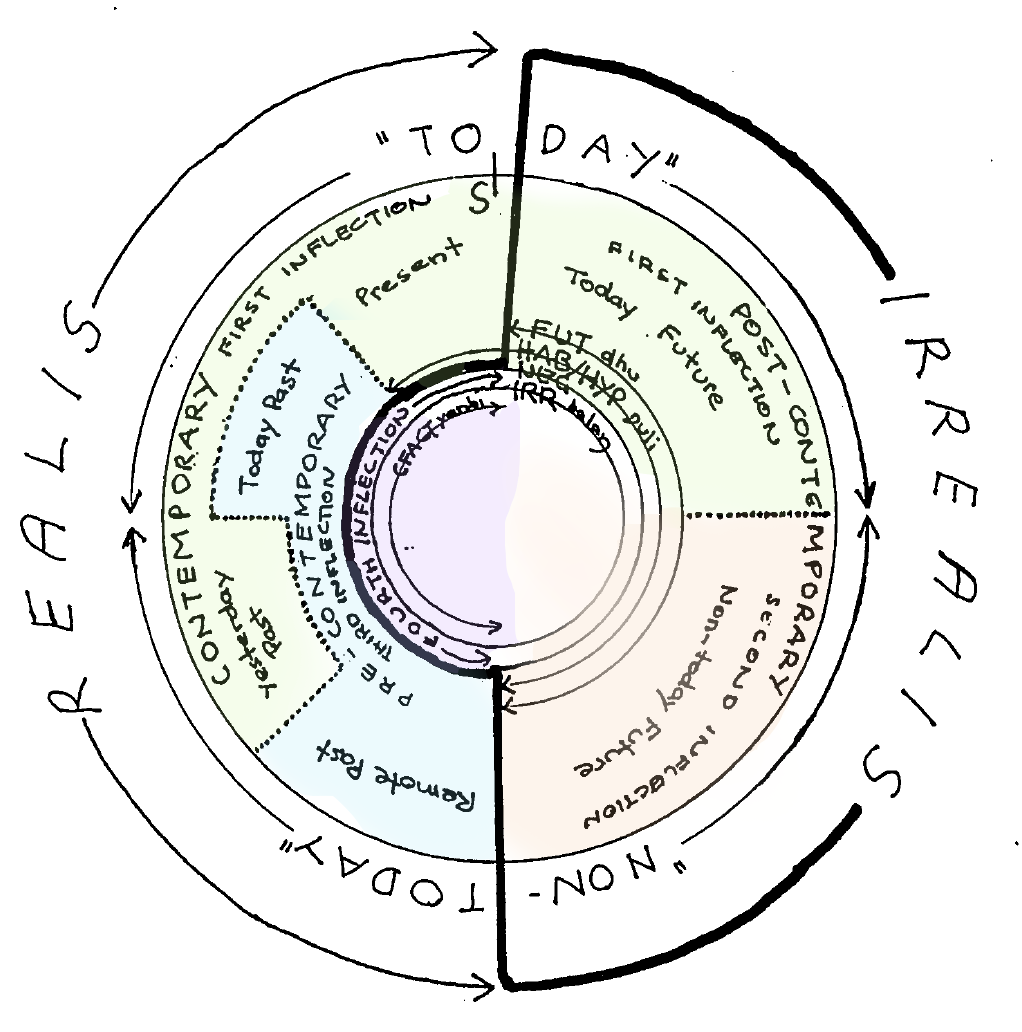
\includegraphics[width=0.8\textwidth]{WilkinsonDiagram362Col}
%	\caption{Melanie Wilkinson's diagrammatic treatment of the distributional properties of Djambarrpuyŋu's four verbal inflections \citeyearpar[362]{Wilkinson1991}. Colourised by author for facilitated presentation of the `domains' of the four inflections.} \label{wilk}
%\end{figure}

\section{Temporal expression in Western Dhuwal(a)}\label{cycTns}
\mcom{similarly, probably too specific a heading --- need either temporal expression above this or cyclicity below this? the section atm includes a discussion of lexical and grammatical aspect.}
\noindent In §\ref{infls}, I provided a description of the distributional facts of the four `inflectional classes' of Dhuwal(a). As we saw, these inflections are in a paradigmatic relation; all finite verbs receive exactly one inflection (caveat the formal identity of some of these inflections in particular verb classes (\textit{sc. }`conjugations.')) In the Western Dhuwal(a) varieties (as in other Yolŋu languages) verbal inflections play a central role in temporal expression. The basic function of inflections \textbf{I} and \textbf{III} in determining the temporal location of a predicate, for example, is shown in (\nextx).

\mcom{These examples are constructed: need to be checked}
\pex\deftagex{minpair}\textbf{Temporal contributions of \textbf{I} and \textbf{III}}\a\deftaglabel{minpair}\begingl\glpreamble \textsc{Present temporal reference} with \textbf{I}//
\gla gäthura ŋarra ga nhina-$\boldsymbol\varnothing$ wäŋaŋura//
\glb today 1s \gls{ipfv}.\textbf{I} sit.\textbf{I} home.\gls{loc}//
\glft`I am staying at home today.'//
\endgl
\a\deftaglabel{pst}\begingl\glpreamble\textsc{Past temporal reference} with \textbf{III}//
\gla gäthura ŋarra ga-na nhina-\textbf{na} wäŋaŋura//
\glb today 1s \gls{ipfv}-\textbf{III} sit.\textbf{III} home.\gls{loc}//
\glft`I was sitting at home (earlier) today.'//
\endgl
\xe

The data in (\getref{minpair}) suggest a present-past distinction encoded by \textbf{I} and \textbf{III} respectively (which is a reasonable analysis for the cognate paradigm in other varieties, see Ch \ref{diaY}). However, as discussed in Ch. \ref{descY}, data of the type shown in (\nextx) quickly throw up problems for a straightforward tense-marking account of these inflections.

\pex \textbf{Temporal contributions of I and III (non-today frame)}
\a\deftagex{MetPst}\deftaglabel{I}\begingl\glpreamble\textsc{Recent past} with \textbf{I}//
%\gla yo barpuru-ny ŋarra \textbf{marrtji}(*-na) shop-lil//
%\glb yes, yesterday{\sc-prom} 1s go-\textbf{I/*III} shop-{\sc all}//
%\glft`Yes, I went to the store yesterday.'//\endgl
\gla Ŋarra ḻuka mänha barpuru//
\glb 1s drink.\textbf{I} water yesterday//
\glft`I drank water yesterday.'\trailingcitation{[BM~20190405]}//\endgl
\a\deftaglabel{III}\begingl\glpreamble\textsc{Remote past} with \textbf{III}//
%\gla yo ŋarra marrtji-\textbf{na} ŋunhawala ŋäthil baman'//
%\glb yes 1s go-\textbf{III} \gls{dist}.\gls{all} before long.ago//
%\glft`Yes, I went there long ago.'//
\gla Ŋunhi ŋarra yothu yäna, ŋarra marrtji-\textbf{na} Sydney-lili//
\glb \gls{texd} 1s child only, 1s go-\textbf{III} Sydney.-\gls{all}//
\glft`When I was a kid, I went to Sydney.'\trailingcitation{[BM~20190405]}//
\endgl
\xe



Represented in Figure \ref{wilk}, A major consequence of these data is that, assuming a model where times are naturally, linearly ordered, the intervals to which \textbf{I}- and \textbf{III}-inflected predicates can refer are \textsc{discontinuous.} Figure \ref{TempSchem} schematises this discontinuity.

\begin{figure}[h]\centering\caption{Past-time temporal expression in the Yolŋu Matha varieties of Central Arnhem, demonstrating two descriptive phenomena: (a) cyclicity --- the interspersion/discontinuity of \textbf{I} and \textbf{III} forms and (b) metricality --- the (subjective) division of the past domain between these two forms.\\$\lfloor{\sl today}\rfloor$ indicates the boundaries of the privileged interval {\sl today}. $\boldsymbol{t*}$ is utterance time.}\label{TempSchem}
	
	
	\begin{tikzpicture}[scale=1]
	% draw horizontal line   
%	\draw[<->, line width=.5mm] (0,0) -- (12,0);
	\draw[<-, line width=.5mm] (0,0) -- (9.5,0);	
	%draw rex
	\shade[left color=blue!15!white, right color=green!15!white] (0,0.02) rectangle (4.8,1.5);
	%	\fill[green!10!white] (2.5,0.02) rectangle (4.8,1.5);
	\fill[blue!10!white] (4.8,0.02) rectangle (6.8,1.5);
	\fill[green!10!white] (6.8,0.02) rectangle (9.5,1.5);
%	\fill[orange!10!white] (9.5,0.02) rectangle (12,1.5);
	
	% draw nodes
	\draw (1.25,0) node[below=3pt] {\textbf{}} node[above=10pt] {\textsc{\textbf{III}}};
	\draw (3.675,0) node[below=3pt] {\textbf{}} node[above=10pt] {\textbf{I}};
	\draw (5,0)   node[circle,fill,label=below:$\big\lfloor{\sl today}$] {} node[below=3pt] {\textbf{}} node[above=3pt] {};
	\draw (6.8,0) node[diamond,shade,outer color=black, inner color  = ochre,label=below:$\boldsymbol{t*}$] {} node[below=3pt] {\textbf{}} node[above=3pt] {\textsc{}};
	\draw (5.8,0) node[below=3pt] {\textbf{}} node[above=10pt] {\textsc{\textbf{III}}};	
	\draw (8.15,0) node[below=3pt] {\textbf{}} node[above=10pt] {\textsc{\textbf{I}}};	
%	\draw (10.75,0) node[below=3pt] {\textbf{}} node[above=10pt] {\textsc{\textbf{II}}};	
	\draw (9.5,0)   node[circle,fill,label=below:${\sl today}\big\rfloor$] {} node[below=3pt] {\textbf{}} node[above=3pt] {};
	
	
	%%%braces
	
	\draw [decorate,decoration={brace,amplitude=4pt},xshift=-0pt,yshift=35pt]
	(0.5,0.5) -- (4.5,0.5) node [black,midway,yshift=0.35cm] 
	{\footnotesize metricality};
	
	\draw [decorate,decoration={brace,amplitude=4pt},xshift=-0pt,yshift=40pt]
	(3.5,0.5) -- (9,0.5) node [black,midway,yshift=0.35cm] 
	{\footnotesize cyclicity};
	
	\end{tikzpicture}\end{figure}




Previous accounts of this phenomenon have described the data in terms of the oppositions between two binary categories: ``contemporary'' (\textbf{I}) vs. ``precontemporary'' (\textbf{III}) tense marking and a contextually provided ``today'' and ``non-today'' reference frame. This interaction was shown in Table  \ref{GlaswegianTR} (\textit{p.} \pageref{GlaswegianTR}), each cell of which is represented by one of the datapoints in (\getref{minpair}-\getref{MetPst}). This schema introduced by \citet{Glasgow1964} for Burarra data [\gls{bvr}], terminology adopted and adapted by numerous other authors for languages of Arnhem Land \citep[see][]{Eather2011,Green1987,Green1995}.


While, as cited above, \citet[89]{Comrie1985} recommends `appeal to its rarity as an excuse for according it [cyclic tense] marginal status in the theory', the current work contends that we should be desirous of a ``unified'' semantics for each of the verbal inflections. The following sections consider the status of the WD verbal inflections and the relation they bear to temporal expression.



\subsection{Talking about the present}\mcom{This section needs to go somewhere --- specific arguments against an ``aspect-based system'' being at the core of the temporal expression in djr. It's less clear that this is the place.}




\begin{quotation}
	[T]he present is like the window of a railway carriage in which we are sitting. If it were an infinitesimal slit we could not see out properly, and we could not see the countryside laid out with its features in their proper relations; but since it has a width light can enter and we can see each thing in relation to the next and so form for ourselves a picture of the whole...\hfill{\citep[325]{Hamblin1972}}
\end{quotation}



The obligatory occurrence of \textit{ga} `\gls{ipfv}.\textbf{I}' with present-tensed event descriptions has led some authors \citep[e.g.][46]{Heath1980}\footnote{Compare with Table \ref{Infl-Comparisons-Wilk}. Note that Heath suggests that `the [temporal] value of [\textbf{I} and \textbf{II}] depends on context, including the presence of particles. He does not attempt a compositional analysis of the verbal inflections \citeyearpar[38,46]{Heath1980}. Additionally, in various texts \textit{ga} (similarly to \textit{gan}) is glossed as a \textsc{dur}ative marker. He does, however, suggest that in various dialects of Dhuwal (particularly Djapu', the variety that seems to diverge more from the Western Dhuwal(a)) that marking this category is uncommon (and in fact the auxiliary may be inflection-invariant.)} to describe this item as a present-tense marker. As we will see here, this is not the most parsimonious analysis of the Dhuwal(a) inflectional system. The categorical appearance of \textit{ga} (or, in fact, other aspect morphology) is, I will argue, an epiphenomenon of to the well-understood incompatibility between \textsc{present} and \textsc{perfective} (\citealp[66\textit{ff}]{Comrie1976}, \citealp[110]{Smith1997}, \citealp{Malchukov2009} a.o.) in addition to a \textsc{lexical constraint} on the situation aspect (Aktionsart) of verbal predicates in W Dhuwal(a). An analysis that treats \textit{ga} as encoding a present tense presupposition, in fact can be dismissed by data such as those in (\nextx) where the reference time for each sentence is clearly located in the past of utterance time.

\pex \textbf{\textit{ga} `\textsc{ipfv.I}' in past-referring sentences}
\a\begingl\gla barpuru ŋali \textbf{ga} waŋanha-mi-rr//
\glb yesterday 1d.\textsc{incl} \textbf{\gls{ipfv}}.\textbf{I} speak.IV-\gls{recip}-\textbf{I}//
\glft`We were speaking to each other yesterday.'\trailingcitation{[AW~20190426]}//\endgl
\a\begingl\gla nhä nhe \textbf{ga} djäma barpuru?//
\glb what 2s \textsc{\textbf{ipfv}}.\textbf{I} work yesterday//
\glft`What were you doing yesterday?'\trailingcitation{[DhG 20190413]}//\endgl
\a\begingl\gla ŋäthili dhuŋgarra-y djäma ŋarra \textbf{ga} shopŋura//
\glb previous year-\textsc{erg} work 1s \textsc{\textbf{ipfv.I}} shop.\gls{loc}//
\glft`Last year I was working at the shop.'\trailingcitation{[BM~20190416]}//\endgl
\xe

In fact, there is significant evidence that all verbal predicates in Dhuwal(a) (or at least those varieties spoken in Ramingining) are lexically event-denoting. This has already been suggested by the data in (\getref{psychPreds}), where stative concepts like \textsc{be sick} and \textsc{be tired} appear to be implicated by (de-nominal) \textbf{III}-inflected verb forms (literally \textit{rirrikthurruna} ``I became sick''$ \rightsquigarrow $ `I am (currently) sick'). This is shown in (\getfullref{sick.III}). Explicit predications about current states may require periphrasis (e.g. the nominal predication in \getfullref{sick.dhaka}). Meanwhile, the \textit{ga}-marked \textbf{I} form (\getref{sick.I}) results in a state-change reading. Relatedly, in (\getref{hungry}), \textit{gutharra} is understood to be in the process of asking for food in view of her current `hunger' state. That her hunger holds in the present is an implicature of a past-tensed eventuality of `becoming hungry.'

\pex\textbf{\textit{rirrikthun} `sick': state or state-change denoting?}
\a\deftagex{sick}\deftaglabel{III}\begingl\gla Ŋarra rirrik-thu-\textbf{rruna}//
\glb 1s sick-\gls{vblzr}-\textbf{III}//
\glft`I'm sick.'\trailingcitation[BM~20190405]//\endgl

\a\begingl\gla Ŋarra dhäkay-ŋänha-mirri rirrikthu-\textbf{n}\deftaglabel{dhaka}//
\glb 1s feeling.\gls{erg}-hear.\textbf{IV}-\gls{prop} sick-\textsc{incl}-\textbf{I}//
\glft`I'm feeling sick.'\trailingcitation[BM~20190405]//\endgl


\a\begingl\gla Dhuwala ŋarra ga rirrikthu-\textbf{n}
\deftaglabel{I} //
\glb  \gls{prox} 1s \textsc{ipfv.\textbf{I}} sick-\gls{inch}-\textbf{I}//
\glft`I'm getting sick.'\trailingcitation[BM~20190405]//\endgl

\xe

\mcom{this example is the guf title from Waymamba Gaykamaŋu's 20171208 translation of a djr text composed by Galathi Dhurrkay from 20141015}\ex\begingl\glpreamble\textbf{\textit{djaṉŋarrthin} `hungry': post-state \& present-predication}\deftagex{hungry}//
\gla Gutharra-y ga waŋa märi-nha ŋatha-wa bili ŋayi djaṉŋarr-thi-na//
\glb \gls{da}\gls{ch}-\gls{erg} \gls{ipfv}.\textbf{I} speak.\textbf{I} \gls{mo}\gls{mo}-\gls{acc} food-\gls{dat} because 3s hunger-\gls{inch}-\textbf{III}//
\glft`\textit{Gutharra} asks \textit{märi} for food because she's hungry.'\trailingcitation{[]}//\endgl\xe


As well as derived (de-nominal) verbs, simplex verbal stems with psychological (incl. perception) semantics --- e.g. \textit{nhäma} `see', \textit{dharaŋan} `understand', \textit{guyaŋa} `think' --- seem to lexically encode \textit{events}. When predicating of a presently-holding state, these verbs require imperfective marking. Otherwise, a \textbf{III}-inflected form appears to implicate that the post-state of the event described by the predicate still holds. This is shown for \textit{nhäma} `see' in (\nextx) below. In these cases an (eventive) predicate denotes a bounded, telic type of situation: an \textsc{achievement} in the sense of \citet{Vendler1957} or \textsc{happening} per \citet{Bach1986}. %all require explicit imperfective marking when predicating of a present state. 

\pex\textbf{\textit{nhäma} `see': perception as a telic event}
\a\begingl\gla Ŋarra nhä-\textbf{ŋala} wuŋgan//
\glb 1s see-\textbf{III} dog//
\glft`I see the dog.'\trailingcitation{[BM~20190405]}//\endgl
\a\begingl\gla Ŋarra \#(\textbf{ga}) nhä-\textbf{ma} wuŋgan dhiyaŋu bala//
\glb 1s \#(\textsc{\textbf{ipfv.I}}) see-\textbf{I} dog \gls{texd}.\gls{erg} \gls{mvtawy}//
\glft\textbf{Intended. }`I'm watching the dog currently.'\trailingcitation{[BM~20190405]}//\endgl\xe


%Consequently, futurate readings emerge when context provides a `today frame' to a \textbf{I} inflection, as was shown in (\getfullref{futI.marrtji}) -- here repeated as (\nextx).
%
%\pex\deftagex{plan}\begingl\gla ŋarra marrtji-n dhiyaŋu-n bala//
%\glb 1s go-\gls{seq} \textbf{\gls{prox}.\gls{erg}}-\gls{seq} \textbf{\gls{mvtawy}}//
%\glft`I'm going now.'\trailingcitation{\citep[256]{Wilkinson1991}}//\endgl
%\xe
%
%In (\getref{plan}), the cooccurrence of an eventive predicate \textit{marrtji} `go' without imperfective marking appears to lead to a futurate reading. If eventive predicates receive default perfective interpretations in Dhuwal(a), a present-inflected event is likely to license a \textsc{plan} type reading (following \citealt{Copley2009}.)

Additionally, \citet[557]{Wilkinson1991} describes a `minor [word] class' : the ``adjectival''-predicates. These three commonly-occurring predicates are all lexical statives (whose semantics correspond to those for the category of \textit{psych verbs} cross-linguistically): \textit{djäl} `want, like', \textit{marŋgi} `know' and \textit{dhuŋa} `not.know.'\footnote{These verbs also have a range of circumstantial modal readings (ability, bouletic, preferential), perhaps predictable given their propositional attitude-type semantics. Examples of these readings are given in \getref{dhuŋa}, and additionally in Wilkinson 1991:648.} Morphosyntactically, each takes an intransitive frame (selecting for a \textsc{nom} experiencer and \textsc{dat} theme) and resists co-occurrence with verbal particles (\textit{i.e.} aspect marking). Like other nominal elements, productive suffixation (notably \textit{-thirr(i)} `\gls{inch}.\textbf{I}', \textit{-kum(a)} `\gls{caus}.\textbf{I}' and \textit{-thun/-'yun} \gls{vblzr}.\textbf{I}) is available to derive verbal forms (intransitive and transitive, respectively). The contrast between the two continuations in (\getfullref{latjin}) below shows incompatibility between stative predicate \textit{djäl} `like' and aspect marking (\getref{latjin.bare}), which, conversely, is obligatory for the derived verbal predicate in (\getref{latjin.inch}). A similar effect is shown for the predicate \textit{marŋgi} `know' (\getref{marŋgi}), where the eventive (``change of state'') semantics of the verbal predicate \textit{marŋgithirr(i)} `learn $ \approx $ come to know' are transparent.


\pex\deftagex{latjin}\textbf{Stative \textit{djäl} `like, want': incompatible with \textit{ga }`\gls{ipfv}' marking}\\
\begingl\gla Ŋäthili ŋarra bäyŋu \textbf{djäl} ḻatjin'-gu...//
\glb previously 1s \gls{negq} like mangrove.worm-\gls{dat}//
\glft`I didn't used to like \emph{ḻatjin}... //\endgl
\a\deftaglabel{bare}\begingl\gla \nogloss{...} dhiyaŋunydja~bala ŋarra (*ga) \textbf{djäl} ḻatjin'-gu//
\glb now 1s (*\textsc{ipfv}) like \textit{ḻatjin}-\gls{dat}//
\endgl
\a\deftaglabel{inch}\begingl\gla \nogloss{...} dhiyaŋunydja~bala ŋarra *(ga) \textbf{djäl-thi-rri} ḻatjin'-gu.//
\glb now 1s *(\textsc{ipfv}) like-\gls{inch}-\textbf{I} \textit{ḻatjin}-\gls{dat}//
\glft`...now I do like them.'\trailingcitation{[DhG~20190417]}//\endgl
%\a\begingl\gla ŋarra djäl ḻatjin'-gu yurru ŋarra yaka djälthina//
%\glb 1s like mangrove.worm-\gls{dat} but 1s \gls{neg} like-\gls{inch}-\textbf{IV}//
%\glft`I like \textit{ḻatjin}, but I didn't want (any).'\trailingcitation{[AW~20190422]}//\endgl
\xe





\pex\deftagex{marŋgi}\textbf{Stative \textit{marŋgi} `know' incompatible with \textit{ga }`\textsc{ipfv}' marking}
\a\begingl\gla Ŋarritjan (*ga) \textbf{marŋgi} Baŋaḏi-wa//
\glb \gls{malk} (*\gls{ipfv}.\textbf{I}) know \gls{malk}-\gls{dat}//
\glft`\textit{Ŋarritjan} knows \textit{Baŋaḏi}.'\trailingcitation{[DhG~20190417]}//\endgl
\a\begingl\gla Dhiyaŋu~bala Wamuttjan \textbf{ga} \textbf{marŋgi-thi-rri} Bäŋaḏi-wa//
\glb now \gls{malk} \gls{ipfv}.\textbf{I} know-\gls{inch}-\textbf{I} \gls{malk}-\gls{dat}//
\glft`\textit{Wamuttjan} is getting to know (learning about) \textit{Baŋaḏi}.'\trailingcitation{[DhG~20190417]}//\endgl\xe

Similarly, the stative predicate \textit{dhuŋa} resists aspectual marking. (\getfullref{dhuŋa.swim}) shows the establishment of a (remote past) reference time with a subordinate temporal clause while (\getref{dhuŋa.dance}) shows how the corresponding verb form (as with its counterparts in the examples above) requires explicit imperfective marking for a present stative predication.


\pex\deftagex{dhuŋa}\textbf{Stative \textit{dhuŋa} `ignorant'}
\a\deftaglabel{swim}\begingl\gla Ŋunhi ŋarra yothu yän, ŋarra \textbf{dhuŋa} ḻupḻupthunara-w//
\glb\gls{texd} 1s child only, 1s ignorant swim.\textbf{IV}-\gls{dat}//
\glft`When I was a kid, I couldn't swim.'\trailingcitation{[AW~20190429]}//\endgl
\a \deftaglabel{dance}\textsc{context.} I decline an invitation to dance at a forthcoming ceremony.\beginsubsub\b{i.}\begingl \gla \nogloss{---} Ŋarra \textbf{dhuŋa} girritjinara-w //
\glb 1s ignorant dance.\textbf{IV}-\gls{dat}//
\endgl
\b{ii.}\begingl\gla \nogloss{---} Bili nhe \textbf{*(ga)} \textbf{dhumbal'yu-n} \upshape{for the step/the beat}.//
\glb because 2s *(\gls{ipfv}.\textbf{I}) not.know-\textbf{I}//
\glft --- `I don't know how to dance (at the \textit{buŋguḻ}).'\\
--- `Because you don't know the steps, the beat.'\trailingcitation{[AW~20190429]}//\endgl
\endsubsub\xe


The behaviour of these nonverbal predicates (i.e. their resistance to explicit aspect marking) is consistent with cross-linguistic behaviour of stative predicates.\footnote{By way of examples:\begin{itemize}\item The infelicity on progressive-marking of stative verbs in English (\citealp[e.g.][55]{Dowty1979}, \citealp[205]{Taylor1977} a.o.)
		\item Whereas dynamic verbs in Russian all appear with imperfective and (inflected) perfective stems, the latter is unavailable for stative verbs \citep[227]{Smith1997}.
		\item In Navajo, `overt viewpoint [aspectual] marking' only occurs in non-stative sentences\citep[297]{Smith1997}.\end{itemize}}
	
%\citeauthor{Dowty1986}'s (1986) analysis of the 


So far in this section, we have seen evidence of an organising principle in W. Dhuwal(a) where all verbal (inflecting) predicates lexically encode eventive (dynamic) situations which are temporally bound (i.e. have endpoints). This principle is formulated in (\nextx).



\ex \textbf{\textsc{verbal stems as inherently eventive in W. Dhuwal(a)}}\deftagex{IEC}\\
W. Dhuwal(a) verbal predicates denote properties of events.
\xe


As mentioned above, situations that obtain in the present `must be open and unbounded, without endpoints... ongoing events; particular states and general states' \citet[230]{Smith2008}. This is formulated as a basic pragmatic principle as the constraint in (\nextx).

\ex  \textsc{\textbf{the \textit{Bounded Event} constraint}}\deftagex{BEC}\\
Bounded situations may not be located in the present.\hfill\citep[231]{Smith2008}
\xe


A consequence of the interaction of the two contraints in (\getref{IEC}) and (\getref{BEC}) is that\textbf{ unmodified verbal stems} (which denote bounded, eventive situations) \textbf{are} \textbf{infelicitous with present temporal reference}. As we have seen here, W. Dhuwal(a) encodes stative situation types by way of three strategies:
\pex[nopreamble]\deftagex{stat-predn}\a nominal predications,
	\a post-state implicatures (through both derived and simplex past-denoting predicates) or 
	\a the explicit marking of imperfectivity (normally with inflecting auxiliary \textit{ga} or stance/motion verbs (see §~\ref{ipfvty}) or with the habitual marker \textit{ŋuli}.)\xe

In fact, \citet{Dowty1979,Dowty1986} --- along with \citet{Taylor1977} --- defines criteria for progressive marking and stative sentences which theorise that ``no matter what the aspectual class of the lexical verb'' any progressive-marked sentence will be stative. These conditions as laid out in \citet[42-4]{Dowty1986} are recapitulated in (\getref{AspClForm}) below:\mcom{It's not super clear that this doesn't belong in a lit reviewy section which then gets cross-referenced here. Also the semantics for the \textsc{prog} is fine for current purposes (may not as we continue forward but it gets the imperfective-stative theorem)}
\pex\a \deftagex{AspClForm}\textbf{\textsc{stative criterion} (the `subinterval property')}\\
$ \textsc{stative}(\varphi) \leftrightarrow \varphi(i)\to\forall i'\big(i'\sqsubseteq i\to\varphi(i')\big)$\\
A sentence $ \varphi $ is stative iff it follows from the truth of $ \varphi $ at $ i $ that $ \varphi $ is true at all of $ i $'s possible subintervals $ i' $\deftaglabel{stat}

\a\textbf{\textsc{A semantics for the progressive}}\\
$  \textsc{prog}(\varphi)(i)\leftrightarrow\exists i'\big(i'\sqsupset i \wedge\varphi(i')\big)$
The progressive form of $ \varphi(i) $ is true iff there is some proper superinterval $ i' $ at which $ \varphi $ is tue.\deftaglabel{prog}
\xe

That progressive-marked sentences necessarily meet the stative criterion is deduced in (\nextx) below.


\pex[exno=68]\a[label=c.]\textbf{\textit{Theorem.}} \textit{Progressive-marked sentences entail stativity (the subinterval property holds.)}\\
\begin{tikzpicture}[baseline,node distance=.1ex]
\node (1) {$\textsc{prog}\varphi (i) $};
\node (2) [below=of 1] {$\exists i'\sqsupset i \wedge\textsc{prog}\varphi(i')$};
\node (3) [below=of 2] {$\forall i''(i''\sqsubseteq i\to i''\sqsubseteq i')$};
\node (4) [below= of 3] {$\textsc{prog}\varphi(i'')$};
\node (5) [below=of 4] {$\textsc{prog}\varphi(i)\to\forall i''\big(i''\sqsubseteq i\to\textsc{prog}\varphi(i'')\big)$};
\node (6) [below=of 5] {$\textsc{stat\big(prog}\varphi(i)\big) $};
%\path (BvC) edge[-] (B);
%\path (BvC) edge[-] (C);
\node (1n) [left=3cm of 1] {i.};
\node (2n) at (1n |- 2) {ii.};
\node (3n) at (1n |- 3) {iii.};
\node (4n) at (1n |- 4) {iv.};
\node (5n) at (1n |- 5) {v.};
\node (5n) at (1n |- 6) {vi.};
\node (r1) [right=3cm of 1, label=right:{\textit{\textsc{premise}}}] {};
\node (r2) at (r1 |- 2) [label=right:{(\getfullref{AspClForm.prog}), i.}] {};
\node (r3) at (r1 |- 3) [label=right:{def. $\sqsubseteq$, ii.}] {};
\node (r4) at (r1 |- 4) [label=right:{(\getfullref{AspClForm.prog}), i,ii i.}] {};
\node (r5) at (r1 |- 5) [label=right:{i,iii,iv}] {};
\node (r6) at (r1 |- 6) [label=right:(\getfullref{AspClForm.stat}) $ \qed $]	{};
\end{tikzpicture}
\xe

All this is to suggest that all W. Dhuwal(a) verbal predicates denote properties of bounded events, a class of situations that are incompatible with present temporal reference. Nominal predication (including the adjectival and locative predicates) and sentences with imperfective marking denote states. Consequently, all verbal predicates obligatorily cooccur with \textit{ga} `\gls{ipfv}.\textbf{I}' when referring to a presently-holding state. 


\subsection{Modelling present predication}\mcom{Unsure about the implications of this direction rather than (the prima facie perhaps more intuitive/standard claim) that verb stems select for inflection i.e. are\\In fact this doesn't make sense really if the inflections are just going to quantify over intensions..... it would have to be the stem...hnnngggg} This apparent lexical constraint can be modelled in the semantics for the W. Dhuwal(a) verbal inflections. %Under such an analysis, each inflection can be interpreted only with respect to \textit{eventive predicates.} As we will see, this can be modelled by having c	{\color{gray!90}This is modelled by treating each inflection as presupposing an event variable which it situates with respect to time/modality.} 
Consequently, our ontology will contain a \textit{domain of eventualities} $ D_\varepsilon $ partitioned into stative and eventive subtypes. Variables over events will be notated $ e $, over states $ s $, summarised in (\nextx)

\ex $ D_\varepsilon \begin{cases}
\mathcal E_\epsilon	& \text{eventive situations}\hspace{.5in} e,e',e'',e'''\\
\mathcal E_s	& \text{stative situations}\hspace{.6in} s,s',s'',s'''...
\end{cases} $\xe


Verbal (inflecting) predicates are then understood to denote properties of events $ \langle \varepsilon_e,t\rangle $. These obligatorily combine with an aspectual operator (e.g. \textit{ga} `\gls{ipfv}' or $ \varnothing $ `\gls{pfv}') %\footnote{Other aspectual operators discussed in Chapter 4, notably \textit{ŋuli} `\gls{hab}'} may also introduce a time variable. } 
to yield a predicate of intervals $ \langle\imath,t\rangle $. Following the neo-davidsonian approach assumed in \citealt{Deo2015}, these operators ``map properties of [events] to sets of intervals relative to which these predicates are instantiated via existential quantification over the Davidsonian event variable'' (11).


The differential contributions of each inflection are investigated in detail in the remainder of this chapter, although the basic structure of each is taken to
% \textbf{relate an eventive situation} to \textbf{the context of evaluation}. 
The denotation in (\nextx) is intended to capture these shared elements (although will be significantly revised through this chapter.)

\ex \textbf{Meaning kernel for the inflectional categories} (\ul{temporal contribution}: to be revised)\\
\denote[i*]{\textsc{infl}}$ =\lambda P:\exists e\in\mathcal E_\epsilon[P(e)]\,.\,\tau(e)\,\mathcal{R}\,i* $\\
The category of \textsc{inflectional suffixes} in W Dhuwal(a) presupposes that the situation described by the predicate $ P $ is eventive $ e $ and (depending on the nature of the inflection) relates the runtime of that event $ \tau(e) $ to the evaluation time $ i* $.
\xe
\mcom{No this is changed now based on the fact that the inflections are gonna be taken to compose with properties of intervals (i.e. the semantic domain of \textbf{AspP})}


%A consequence of this denotation is that the four verbal inflections in Djambarrpuyŋu are to be modelled as properties of events $\langle\varepsilon_e,t\rangle $. 

Above, we saw examples of derived (de-nominal) verbs with change-of-state semantics. Whereas we have seen that nominal predicates are often used to encode stative situation types productive suffixation --- \textit{-ˀThu-} `\gls{vblzr}', \textit{-Thi-} `\gls{inch}', \textit{-ku-/-Thi-} `\gls{tr}' and \textit{-mara-} `\gls{caus}'\footnote{The forms of these  suffixes are subject to significant allomorphy. I generalise over each category following the proposals of \citet[§ 7.5]{Wilkinson1991}.} --- derives inflecting verbal predicates with accordingly eventive semantics.\footnote{According to \citet{Dowty1972,Dowty1979}, statives are in fact the ``basic'' predicate type which composes with a finite number of [situation] aspectual operators/connectives to yield predicates of events.} \citet{Wilkinson1991} demonstrates the paradigmatic relation between these predicates. Some examples are given in Table \ref{sit-deriv} below (predominantly from her description) and formal proposals for the contributions of a number of these operators are given in (\nextx) below.


\begin{table}[h]
\centering	\caption{Morphological derivation of inflecting eventive predicates}\label{sit-deriv}
	\begin{tabular}{>{\em}ll>{\em}ll}
\toprule
	\multicolumn{2}{c}{\textbf{\textsc{stative predicate}}} & \multicolumn{2}{c}{\textbf{\textit{-Thi }`\gls{inch}'}}        \\
		baṉḏany         & `shallow'           & baṉḏany-dhin  & `dry up.\textbf{I}'              \\
		gorrmur         & `hot'               & gorrmur-'yin  & `get hot, have fever.\textbf{I}' \\
		buthalak        & yellow              & buthalak-thin & `be(come).yellow.\textbf{I}'       \\\midrule
		\multicolumn{2}{c}{\textbf{\textsc{stative predicate}}} & \multicolumn{2}{c}{\textbf{\textit{-Thu} `\gls{vblzr}'}}       \\
		warwu           & `sorrow'            & warwu-'yun    & `worry, feel.upset.\textbf{I}'     \\
		bilma           & clapstick           & bilma-'yun    & `use.clapstick.\textbf{I}'       \\
		ŋaḏi            & `discontent'        & ŋaḏi-'yun     & `sulk.\textbf{I}'                \\\midrule
		\multicolumn{2}{c}{\textbf{\textsc{stative predicate}}} & \multicolumn{2}{c}{\textbf{\textit{-ku/-Tha }`\gls{tr}'}}    \\
		baṉḏany         & `shallow'           & baṉḏany-kuma & `dry.\textbf{I}'                 \\
		dhunupa         & `straight'          & dhunuka-kuma & `put.right.\textbf{I}'           \\
		galki           & `close'             & galki-kuma   & `bring.close.\textbf{I}'        \\\bottomrule
	\end{tabular}
\end{table}

\pex\deftagex{sit-deriv}\textbf{The functions of verbal derivation}\a \textbf{A semantics for \textit{-Thi} `\gls{inch}oative' }\beginsubsub
\b{i.} % \textbf{The operator \textsc{become} (adapted from \citealt{Dowty1972,Dowty1979})}
$ \textsc{become}\,\varphi(i)\underset{\text{def}}{=}\exists j[j\underset{\text{init}}{\sqsubseteq}i\wedge\neg \varphi(i)]\wedge\exists k[k\underset{\text{fin}}{\sqsubseteq}i\wedge \varphi(i)]$\\
A formula  \textsc{become} $ \varphi $ is true at $i$ if $\varphi $ is both: true at a final subinterval $k$ and false at an initial subinterval$ (j) $. \hfill \citep[Adapting liberally from][]{Dowty1979}\\This is diagrammatised in Figure \ref{become-dia}. 
 \footnote{This predicate, labelled \textsc{come about} in Dowty's \citeyear[45ff]{Dowty1972} dissertation appeals to a dense series of moments in time before being updated to an interval semantics in \citeyear[139ff]{Dowty1979}, following \citet{Bennett}. Where Dowty appeals to an initial/final overlap relation ($ \circ $), here I replace that with notions of initial/final subintervals which seems to partially avoid some of the problems he discusses (140-2). Nevertheless, as formulated here the definition is still too weak and does permit for $ i $'s theoretically unbounded length. Dowty partially solves this by stipulating that $ i $ is the largest interval for which these properties hold.}
\b{ii.} \denote{\textit{ -Thi }}$_{\langle\langle\varepsilon_s,t\rangle,\langle\varepsilon_\epsilon,t\rangle\rangle}=\lambda P^s.\lambda e[\textsc{become}(P^s)(e)]  $

\textit{-Thi} `\gls{inch}' is a situation operator which takes a property of states $ P^s \subseteq \mathcal E$ and returns the set of events \textsc{become} $ P^s\subseteq\mathcal E_\epsilon$.
\endsubsub
\a\textbf{A semantics for  \textit{-Thu} `\gls{tr}ansitiviser'}\\%\beginsubsub
	\denote{\text{-Thu}}$_{\langle\langle\varepsilon_s,t\rangle,\langle e,\langle\varepsilon_e,t\rangle\rangle\rangle}=\lambda y\lambda P^s.\exists e[\textsc{cause}(y,\textsc{become}(P^s)(e))]$
	
	\textit{-Thu} `\gls{tr}' is a situation operator which takes a property of states  $ P^s $ and returns a function from individuals (agents/causers) to events $ (\lambda y. y\,\textsc{cause}\,\textsc{become}\,P^s\subseteq E\times\mathcal E_\epsilon)$ %\endsubsub
	
\xe\mcom{need to revise \textit{-Thu} at least}

Relevantly for current purposes, the nominal predicates in the first column of table \ref{sit-deriv} are all state-denoting and, consequently, are incompatible with verbal inflections and imperfective marking (sc. \textit{ga}). As (\getref{sit-deriv}) shows, on a neo-Dowtian treatment, when verbs are derived from these stative predicates, an eventive interpretation is generated. This captures the intuition that \textbf{predicates of events, in effect, denote changes in state over time} (``dynamicity''). 

\begin{figure}[h]
\caption{Truth conditions for state change operator \textsc{become} (adapted from \citealp{Dowty1979})}\label{become-dia}\centering
\begin{tikzpicture}
\draw[<->, line width=.5mm] (0,0) -- (6,0);
\draw (3,.25) node[color=forest] {$ \boldsymbol i $};
\filldraw[nearly transparent,cyan](3,0)		ellipse [x radius=2cm,y radius=.8cm];
\draw (2,.17) node[color=blue,yshift=.1cm] {$j$};
\filldraw[nearly transparent,yellow,xshift=0.2cm](1.6,0)		ellipse [x radius=.8cm,y radius=.5cm];
\draw (4.25,.2) node[color=red] {\textbf{$k$}};
\filldraw[nearly transparent,yellow,xshift=-0.2cm](4.4,0)		ellipse [x radius=.8cm,y radius=.5cm];


\draw [decorate,decoration={brace,amplitude=6pt},xshift=-0pt,yshift=40pt] %%%BECOME BRACE
(1.2,0) -- (4.8,0) node [black,midway,yshift=0.375cm] 
{\footnotesize \textsc{become} $P^s$};

\draw [decorate,decoration={brace,amplitude=4pt},xshift=-0pt,yshift=25pt] %%%% HOLD BRACE
(3.5,-0.0) -- (4.8,-0.0) node [black,midway,yshift=0.35cm] 
{\footnotesize $ P^s $};

\draw [decorate,decoration={brace,amplitude=4pt},xshift=-0pt,yshift=25pt] %%%%NOT HOLD BRACE
(1.2,-0.0) -- (2.5,-0.0) node [black,midway,yshift=0.35cm] 
{\footnotesize  $ \neg P^s $};

\end{tikzpicture}
\end{figure}

This treatment further evinces the infelicity of present-tensed eventive predication with which we have been concerned so far in this section. Given that eventive predicates of the \textsc{become}-type assert a \textbf{state-change} over time, reference to an entire, bounded eventuality of this type must be located within an extended interval in which both $ P $ and $ \neg P $ hold.

In this subsection we have made the following observations:
\begin{itemize}
	\item Dhuwal(a) verbal predicates denote properties of events;
	\item Eventive predication is incompatible with present-reference;
	\item Properties of states (which are present-tense compatible) are predicated by the three strategies given in (\getref{stat-predn}), spelled out in (\nextx) below. 
\end{itemize}

\mcom{of course at this stage i haven't included semantics for \textbf{I}/\textbf{III}}
\ex[glwidth=.35\linewidth]\textbf{Strategies for achieving present temporal reference in W Dhuwal(a)}\deftagex{pres-schemata}\\\vtop{\halign{%
#\hfil&& \qquad #\hfil\cr\toprule
\textbf{\textsc{type}}& \textbf{\textsc{example}} & \textsl{\textsc{schema}}\cr\midrule
\textbf{nominal}& \begingl\gla baŋaḏi djawar-mirr//
\glb \gls{malk} tired-\gls{prop}//
\glft $ \lambda s.Jb(s) $//
\endgl& \begin{tikzpicture}[baseline=(current bounding box.north)]
\draw[<->, line width=.5mm] (0,0) -- (6,0);
\draw (3,.25) node[color=forest] {$ \boldsymbol i $};
\filldraw[nearly transparent,cyan](3,0)		ellipse [x radius=2cm,y radius=.8cm];



\draw [decorate,decoration={brace,amplitude=6pt},xshift=-0pt,yshift=30pt] %%%BECOME BRACE
(1.2,0) -- (4.8,0) node [black,midway,yshift=0.375cm] 
{\footnotesize $J(b)$};



\end{tikzpicture}\cr
\textbf{post-state}&\begingl\gla baŋaḏi djawar-yu-rr(una)//
\glb \gls{malk} tired-\gls{vblzr}-\textbf{III}//
\glft $ \lambda s.\exists e[\textsc{become}(Jb)(e)\wedge\tau(e)\prec\textbf{now}](s) $//
\endgl& \begin{tikzpicture}[baseline=(current bounding box.north)]
\draw[<->, line width=.5mm] (0,0) -- (6,0);
\draw (3,.25) node[color=forest] {$ \boldsymbol i $};
\filldraw[nearly transparent,cyan](3,0)		ellipse [x radius=2cm,y radius=.8cm];
\draw (2,.17) node[color=blue,yshift=.1cm] {$j$};
\filldraw[nearly transparent,yellow,xshift=0.2cm](1.6,0)		ellipse [x radius=.8cm,y radius=.5cm];
\draw (4.25,.2) node[color=red] {\textbf{$k$}};
\filldraw[nearly transparent,yellow,xshift=-0.2cm](4.4,0)		ellipse [x radius=.8cm,y radius=.5cm];


\draw [decorate,decoration={brace,amplitude=6pt},xshift=-0pt,yshift=40pt] %%%BECOME BRACE
(1.2,0) -- (4.8,0) node [black,midway,yshift=0.375cm] 
{\footnotesize \textsc{become} $J$};

\begin{scope}
\clip (3,0.0) rectangle(4.7,2);
\draw [decorate,decoration={brace,amplitude=3.975pt},xshift=-0pt,yshift=25pt] (3.5,0) -- (4.8,0) node [black,midway,yshift=0.35cm] 
{\footnotesize  $ J $};
\end{scope};
\draw[-{stealth},yshift=27pt,decorate,decoration={zigzag,amplitude=1pt,segment length=4.75}] (4.67,0) -- (5.3,0) ;
%\path[postaction=decorate,decoration={markings,mark=at position 0.9 with {\arrow{>}}}] decorate[decoration={brace,amplitude=4pt}] { (0,0.7) to (5,0.7)};


\draw [decorate,decoration={brace,amplitude=4pt},xshift=-0pt,yshift=25pt] %%%%NOT HOLD BRACE
(1.2,-0.0) -- (2.5,-0.0) node [black,midway,yshift=0.35cm] 
{\footnotesize  $ \neg J $};

\draw[line width=2mm,nearly transparent] (5.35,1.25) -- (5.3,-.8) node [at end,yshift=-2mm] {\textit{\textsc{now}}};

\end{tikzpicture}\cr
\textbf{imperfective}& \begingl\gla baŋaḏi ga djawar-yu-n//
\glb \gls{malk} \gls{ipfv}.\textbf{I} tired-\gls{vblzr}-\textbf{I}//
\glft $ \lambda s.\exists e[\textsc{become}(Jb)(e)\wedge\tau(e)\sqsupset\textbf{now}](s) $//
\endgl& \begin{tikzpicture}[baseline=(current bounding box.north)]
\draw[<->, line width=.5mm] (0,0) -- (6,0);
\draw (3,.25) node[color=forest] {$ \boldsymbol i $};
\filldraw[nearly transparent,cyan](3,0)		ellipse [x radius=2cm,y radius=.8cm];
\draw (2,.17) node[color=blue,yshift=.1cm] {$j$};
\filldraw[nearly transparent,yellow,xshift=0.2cm](1.6,0)		ellipse [x radius=.8cm,y radius=.5cm];
\draw (4.25,.2) node[color=red] {\textbf{$k$}};
\filldraw[nearly transparent,yellow,xshift=-0.2cm](4.4,0)		ellipse [x radius=.8cm,y radius=.5cm];


\draw [decorate,decoration={brace,amplitude=6pt},xshift=-0pt,yshift=40pt] %%%BECOME BRACE
(1.2,0) -- (4.8,0) node [black,midway,yshift=0.375cm] 
{\footnotesize \textsc{become} $J$};

\draw [decorate,decoration={brace,amplitude=4pt},xshift=-0pt,yshift=25pt] %%%% HOLD BRACE
(3.5,-0.0) -- (4.8,-0.0) node [black,midway,yshift=0.35cm] 
{\footnotesize $ J $};

\draw [decorate,decoration={brace,amplitude=4pt},xshift=-0pt,yshift=25pt] %%%%NOT HOLD BRACE
(1.2,-0.0) -- (2.5,-0.0) node [black,midway,yshift=0.35cm] 
{\footnotesize  $ \neg J $};

\draw[line width=2mm,nearly transparent] (3.35,1.25) -- (3.3,-.8) node [at end,yshift=-2mm] {\textit{\textsc{now}}};

\end{tikzpicture}\cr\bottomrule
}}

\xe

Note that, in the formal and schematic presentation of the sentences in (\lastx), for the sake of exposition, we are abstracting away from a number of important details, including more sophisticated treatments of properties of \gls{ipfv} (e.g. the intensional interpretive component of the \textsc{progressive} as first proposed in \citet{Dowty1977})\footnote{\textit{Viz.} what has been referred to in subsequent literature as quantification over `inertia futures/worlds.'} but crucially also a proper account of the contribution of the verbal inflections \textbf{I} and \textbf{III} in determining temporal reference. We turn to this in the below subsections (§\ref{past-pred}). The derivation in (\nextx) below spells out a number of assumptions about the composition of an eventive predication in Gupapuyŋu.


\mcom{As we've seen, I have the bones of a derivation ready to go on this (assuming I've got the data right). I need to know what existential closure in order to get it to come out. Is it a composition rule distinct from fn appl?}


\pex\textbf{ A compositional derivation of \textit{Baŋaḏi ga djaṉŋarthina}\\`Baŋaḏi is hungry' (lit.~`Baŋaḏi~got~hungry')}

%\begin{tikzpicture}[scale=.9]\tikzset{baseline=(current bounding box.north),every tree node/.style={align=center},level distance=50pt,sibling distance=0pt}
%\Tree [.{\textbf{IP$ _{t} $}\\$ \exists i'\Big[\textbf{III}(i*,i')\wedge\exists i''[i''\sqsupset i' \wedge\exists e\big[\textsc{become-}Jb(e)\circ\tau(e)\circ i'']\big]\Big] $} [.{\textbf{\textit{-na$ _{\langle\langle i,t\rangle,t\rangle} $}}\\$\lambda P.\exists i'[\textbf{III}(i*,i')\wedge P(i')]$} ] [.{$\textbf{AspP}_{\langle i,t\rangle}$\\ $\lambda i\exists i'\big[i'\sqsupset i\wedge\exists e[\textsc{become-}Jb(e)\wedge\tau(e)\circ i']\big] $} [.{\textbf{\textit{ga$_{\langle\langle i,\langle\varepsilon,t\rangle\rangle,\langle i,\langle\varepsilon,t\rangle\rangle\rangle}$}}\\$ \lambda P^\epsilon\lambda i.\exists i'\big[i'\sqsupset i\wedge\exists e[P(e)\wedge\tau(e)\circ i']\big] $} ] [.{$\boldsymbol{\mathcal E}\textbf{P}_{\langle i,\langle\varepsilon_e,t\rangle\rangle}$\\$ \lambda i\lambda e[\lambda s.\textsc{become-}Jb(e)(i)] $} [.{\textbf{PredP}$_{\langle \varepsilon_s,t\rangle}$\\$ \lambda s.J(b)(s)$} [.{\textbf{\textit{baŋaḏi$ _{e} $}}\\$ b $} ] [.{\textbf{\textit{djaṉŋar}}$ _{\langle e,\langle\varepsilon_s,t\rangle\rangle} $\\$\lambda x\lambda s.J(x)(s)  $} ] ] [.{\textbf{\textit{-thi}}$_{\langle\langle\varepsilon_s,t\rangle,\langle i,\langle\varepsilon_\epsilon,t\rangle\rangle\rangle}$\\$ \lambda P^s\lambda i\lambda e.\textsc{become-}P^s(e)(i)  $} ] ] ] ]  
%\end{tikzpicture}
%

\begin{tikzpicture}[scale=.9]\tikzset{baseline=(current bounding box.north),every tree node/.style={align=center},level distance=50pt,sibling distance=0pt}
\Tree [.{\textbf{IP$ _{t} $}\\$ \exists i'\Big[\textbf{III}(i*,i')\wedge\exists i''[i''\sqsupset i' \wedge\exists e\big[\textsc{become-}Jb(e)\circ\tau(e)\circ i'']\big]\Big] $} [.{\textbf{\textit{-na$ _{\langle\langle i,t\rangle,t\rangle} $}}\\$\lambda P.\exists i'[\textbf{III}(i*,i')\wedge P(i')]$} ] [.{$\textbf{AspP}_{\langle i,t\rangle}$\\ $\lambda i\exists i'\big[i'\sqsupset i\wedge\exists e[\textsc{become-}Jb(e)\wedge\tau(e)\circ i']\big] $} [.{\textbf{\textit{ga$_{\langle\langle \varepsilon_\epsilon,t\rangle,\langle i,t\rangle\rangle}$}}\\$ \lambda P^\epsilon\lambda i.\exists i'\big[i'\sqsupset i\wedge\exists e[P(e)\wedge\tau(e)\circ i']\big] $} ] [.{VP$ _{\langle\varepsilon{_e},t\rangle} $\\$ \lambda e.\textsc{become}(\lambda s.Js)(e)\sqcap\vartheta(b,e) $} [.{\textbf{NP}$ _{\langle\varepsilon,t\rangle} $\\$ \lambda e.\vartheta(b,e) $} [.{\textbf{\textit{baŋaḏi}}$ _e $\\$ b $} ] [.{$ \boldsymbol{\underset{nom}{\varnothing}}_{\langle e,\langle\varepsilon,t\rangle\rangle} $\\$ \lambda x\lambda e.\vartheta(x,e) $} ] ] [.{V$ _{\langle\varepsilon_e,t\rangle} $\\$ \lambda e.\textsc{become}(\lambda s.Js)(e)$} [.{\textit{djaṉŋar}$ _{\langle\varepsilon_s,t\rangle}$\\$ \lambda s.Js $} ] [.{\textbf{\textit{-thi}}$_{\langle\langle \varepsilon_s,t\rangle,\langle \varepsilon_e,t\rangle\rangle}$\\$ \lambda P^s\lambda e.\textsc{become}(P^s)(e) $} ] ] ] ] ]     
\end{tikzpicture}


\xe


A number of observations to prosify once this analysis has firmed up a bit:
\begin{itemize}
	\item A nominal predication (PredP) is taken to be a set of states saturated by its theme (absolutive marked argument)
	\begin{itemize}
		\item This has been kind of modified now s.t. the stative property first composes with a verbalising suffix to derive an eventive property.  This probably makes more sense. In a neodavidsonian sort of way I'm kind of abstracting away from how the nominal arguments compose (assuming there's a intersective composition rule $ \boldsymbol\sqcap $ that modifies the event description (Champollion for a summary). I have absolutely zero-commitment to anything beyond events.)
		\item Though this is quite nice in transitive cases where the ergative can be seen as instantiating $ \lambda x\lambda e.\textsc{ag}(x,e) $ and the accusative $ \lambda x\lambda e.\textsc{pat}(x,e) $. For nominative though, we'd probably need two denotations? maybe not. maybe it'd just be typed more generally... let's see.
	\end{itemize}
	\item the verbalising suffix \textit{-thi} as shown in (71) above maps a set of states to events of becoming that state. Given that these require inflection ultimately, this is currently modified as a function from sets of states to functions to time-relativised events.
	\item Viewpoint aspect (\textsc{ipfv}) is a predicate modifier: it takes a set of events and maps it to a predicate of intervals (this meshes with Deo 2015:11)
	\begin{itemize}
		\item consequence of Aspº introducting $ i $ is that i'm gonna need to say that there's a silent \textsc{pfv} operator in complementary distribution with \textit{ga} that introduces a variable over times.
	\end{itemize}
	\item The verbal inflection then maps a predicate (of intervals?) to a proposition, `instantiating these properties at reference time' (ibid.)
	\item {\color{orange}There is a typing problem at the AspP level where maybe there's some existential binding of the event variable. Can we just say that this is one of the things that \textsc{asp} is doing? Or do we need an $ \exists $-closure operator in the syntax (with a Champollion-like semantics, i.e $ \lambda\mathcal E.\exists e[\mathcal E(e)] $)?} I'm still so confused by what the meaning of this could be? It must just be a theory-internal sleight-of-hand right?
	\item {\color{forest} One thing that is likely to simplify the representation here a wee bit (especially when we move up type-wise and start thinking about modality) is using a \textsc{coin} relation (kinda Dowty's \textbf{AT}). This \textbf{does} do the exisntial closure work (acc. Ashwini)}
	\item $ i $  presumably needs to be in the syntax somewhere
\end{itemize}


\pex\mcom{from memory the following verse also had a nice example of nhäŋal}
\begingl\glpreamble \textbf{Dynamic \textit{nhina}}//
\gla walal marrtji-n dhaŋal-ku-ŋal-nha gurtha-n ḻithan-mara-nha-mi-nyara-w-nha walala-ŋgu-wuy walal. Bala ŋayiny Betany dhunupan marrtjin, dhutnha nhinan walala-ŋgal.//
\glb 3p go-\textbf{III} stoke-\gls{caus}-\textbf{III}-\textsc{seq} fire-\gls{prom} dry-\gls{caus}-\gls{nmlzr}-\gls{recip}-\gls{nmlzr}-\gls{dat}-\gls{seq} 3p-\gls{dat}-\gls{assoc} 3p then 3s.\gls{prom} Peter.\gls{prom} straght.\gls{seq} go-\textbf{III} sit.\gls{seq} sit.\textbf{III} 3p-\gls{obl}//
\glft`They were stoking the fire in order to dry each other off. Then Peter came straight in, he sat down with them.'//\endgl
\xe

\pex \begingl\glpreamble \textbf{Continuous reading with \textit{ga} \gls{ipfv}.\textbf{I}}//
\gla \nogloss{...} bili ŋuriŋiyiny ga maŋutji-lakaram ŋunhi God-Waŋarrwuny djeŋarra'mirrnydja Birrimbirr ga nhina-n nhokala.//
\glb because \gls{texd}.\gls{erg}.\gls{ana}.\gls{prom} \gls{ipfv}.\textbf{I} eye-tell.\textbf{I} \gls{texd} God-holy.\gls{prom} bright.\gls{prop}.\gls{prom} spirit \gls{ipfv}.\textbf{I} sit-\gls{seq} 2s.\gls{obl}//
\glft`...because that shows ($ ^{??} $is showing) that the bright spirit of God rests ($ ^{??} $is resting) on you.'\trailingcitation{[\textit{1 Betawuŋ Dhäwu}/1Pet 4:14]}//\endgl\xe

\pex\begingl\glpreamble\textbf{A ḻatjin example from MW (648)}//
\gla wiripu+ny balanda mala marŋgi+mirr ḻatjin+gu ḻuka+nhara+w, ga wiripu+ny mala bäyŋu\ ḻurrkun' marŋgi+ny ḻuka+nhara+w, ga djäl+nydja ḻuka+nhara+w\ ga dharrwa+ny bäyŋu//
\glb certain+PROM white person PL know+PROP mangrove worm+DAT eat+4th+DAT and certain+PROM PL NEGQ few/three know+PROM eat+4th+DAT and want+PROM eat+4th+DAT and many+PROM NEGQ//
\glft`There are some white people who know about eating mangrove worms and others
that do not. A few have eaten (them) and like eating (them) but many don't.'//\endgl

\xe
%In both examples in (\lastx) above, the contribution of \textit{ga} `\textsc{ipfv.\textbf{I}}' is clearly one of viewpoint aspect.


\subsection{Talking about the past}\label{past-pred}



Perhaps the most important distinction between \textbf{I} and \textbf{III} is that events that are predicated as \textbf{including the time of speech} ($\boldsymbol{t*} $) are felicitious only with \textbf{I}, modulo the caveats about post-state predication discussed above.)


At the beginning of this section (in addition to various points in Chapter \ref{descY}), we that past temporal reference for W. Dhuwal(a) eventive predicates can b e established with either \textbf{I} or \textbf{III} inflection. This is clearly demonstrated again by the conjoined sentences in (\ref{coord-pst}) below.

\pex\glpreamble \textbf{Past reference with I and III (conjunction)}\label{coord-pst}//
\a\begingl\gla \nogloss{[} ŋarra ḻuk-\textbf{a} mänha barpuru \nogloss{]} ga \nogloss{[} ŋarra ḻuk-\textbf{ana} mänha dhiyaŋu bili \nogloss{]}//
\glb 1s drink-\textbf{I} water yesterday and 1s drink-\textbf{III} water \gls{prox}.\gls{erg} \gls{cplv} //
\glft`I drank water yesterday and I drank water just before (earlier today).'\trailingcitation{[BM~20190405]}//\endgl


\a\begingl\gla ŋarra barpuru munhagu ŋarra \textbf{ḻuka} djinydjalma ga \textcolor{red}{\textbf{raŋunhaŋala}} bäpawa märr ŋayi dhu \textbf{ḻuka} dhiyaŋu bala goḏarrmirri//
\glb 1s yesterday night 1s eat.\textbf{I} crab and return-\textbf{III} father-\gls{dat} so 3s \gls{fut} eat \gls{prox}.\gls{erg} \gls{mvtawy} morning//
 \glft`I ate some crab last night and this morning brought some back for Dad so that he can eat (some).'\trailingcitation{[BM~20190416]}//\endgl

\xe




Ultimately, we can think of the temporal interval (i.e. range of possible times) that are made available by each inflection can be described as follows (this is schematised in Figure \ref{TempSchem-pst} below.) 
\begin{description}
	\item[\phantom{I}I\phantom{I}]$ \tau(e) \circ$ \textbf{[}\textsc{recent past} \textbf{,} \textsc{end}.day-of-speech\textbf{)}
	\item[III]$ \tau(e) \circ$ \textbf{(}\textsc{remote past} \textbf{,} time-of speech\textbf{]} 
\end{description}

Below, we consider various options for theorising the distributional differences between (and meaning contribution of) \textbf{I} and \textbf{III}.
\subsubsection{\textbf{I} as a present tense marker}


Given that: • \textbf{I} is most clearly distinguished from \textbf{III} by its compatibility with present temporal reference, and also that • cognates of \textbf{I} in closely related Yolŋu varieties clearly realise present tense (see Chapter \ref{diaY}), a possible model of the distribution of \textbf{I} and \textbf{III}, then, analyse \textbf{I} a \ul{\textsc{present-}tense marker}.

Of course, a semantics where the semantic contribution of \textbf{I} restricts the event to overlap with speech-time is untenable in view of \textbf{I}'s compatibility with past-reference. Consequently, an analysis of \textbf{I}-as-\textsc{present} would need to invoke the notion of an \textsc{extended now} (\gls{xnow}, \textit{sc.} ``a time interval reaching back from the time of utterance'' \citep[49]{Cover2010}).\footnote{Note that this definition of \gls{xnow} differs from (i.e. is a subset of) that which is formalised in \citealt[225]{Stump1985}, for whom it is a relation between \textsl{any} arbitary interval $ i $ such that $ \textsc{xnow}(i) = \{i'\mid i'\underset{\text{final}}{\sqsupseteq} i\}$.}  A consequence of an analysis of this type would be that, past-referring utterances with \textbf{I}-morphology must be understood ``not [as locating] a situation at some definite point in the past, but only to offer it as \ul{relevant to the current situation}'', a semantic domain traditionally associated with the \textsc{anterior} or \textsc{perfect} aspect (\citealp[62]{Bybee1994}, underlining added).



%This present-reference for \textbf{I} is then compared against a general past-tense semantics for \textbf{III}.


  Appeal to the notion \gls{xnow} has been deployed in a number of influential accounts of the English present perfect (\citealp[notably][]{McCoard1978, Portner2003} a.o.) to explain both • intuitions about the `current relevance' of present perfect predications and, importantly • ``the present perfect puzzle'' \citep[see][]{Klein1992,Schaden2009}, \textit{sc.} the incompatibility of the present perfect with TFAs for the past (e.g. \textit{*I have eaten a few hours ago}.)

Of course, as we have seen, this reasoning fails to account for the WD data. \textbf{I}, in fact, frequently co-occurs with TFAs for the past (e.g. \textit{barpuru} `yesterday', which does \textit{not }cooccur with \textbf{III} in these varieties.) This is shown again in (\getref{barpuru}):
\pex\deftagex{barpuru}Interactions between \textbf{I} and \textbf{III} and recent past-denoting TFA \textit{barpuru}\a\begingl\deftaglabel{I}\gla ḏirramuwal yothuwal bäpa'mirriŋuy rrupiya barpuru \textbf{djuy'yu-n}, \textbf{märr} \textbf{barpuru} + ga \textbf{barpuru} \textbf{buna}-ny dhiyal-nydja.//
\glb man.\gls{obl} child.\gls{obl} father.\gls{kinprop}.\gls{erg} money yesterday send-\textbf{I} kinda yesterday and yesterday arrive.\textbf{I}-\gls{prom} \gls{prox}.\gls{loc}-\gls{prom}//
\glft`The father sent money to the boy recently and it arrived here yesterday.'\trailingcitation{\citep[343]{Wilkinson1991}}//
\endgl

\a\deftaglabel{III}\begingl\gla ŋarra ga-na \textbf{ḻuka-na} barpuru//
\glb 1s \gls{ipfv}-\textbf{III} consume-\textbf{III} yesterday//
\glft\textsc{Intended.} `I was drinking water yesterday.'\trailingcitation{[DhG~20190405]}//\endgl


\xe

Given that TFAs for the past ought to be compatible with past-tense marking and incompatible present-tense marking, the \textsc{pres/pst} analysis of these inflectional categories makes false predictions of infelicity with \textbf{I}  (\getfullref{barpuru.I}) and felicity with \textbf{III} (\getfullref{barpuru.III}). On the basis of this data we can dismiss a treatment that treats \textbf{I} as \textsc{pres}-denoting and accounts for the \textit{recent past} uses as emerging out of a \textsc{perfect/anterior} reading of the present.

Relatedly, the relationship between (erstwhile) present perfect constructions and past temporal reference. in Peninsular Spanish varieties, ``perfective uses of the [present] perfect are restricted to certain temporal contexts, such as describing events that happened during the `today' or `yesterday' intervals... [whereas the \textit{préterito} is] found in virtually any type of context when past reference is made'' (\citealp[72]{Howe2006}, also \citealp[115ff]{CurelliGotor1990} for Catalan.) This is argued to be an instantiation of a grammaticalisation pathway where the distribution of a particular grammatical marker acquires \textsc{perfect} meaning before further developing into a \textsc{perfective} or \textsc{past} tense operator.\footnote{The ``pathway'' \textsc{perf $ \to $ pfv} has been referred to as the ``Aoristic drift'' \citep{Schaden2009,Schaden2012}. See \citep{Schwenter1994} for the Alicante variety of Peninsular Spanish, \citep{Condoravdi2014} for the instantiation of this pathway in Indo-Aryan.} This phenomenon and its relevance for an analysis of the Yolŋu data presented here is treated below (§ \ref{hod}).





\subsubsection{Disjunctive presuppositions}
A consequence of these data for theories of tense is that, if we assume an ``off-the-shelf'' account of tense marking as encoding a presupposition about the relation between a contextually-provided reference time and the time of speech, we are left with the disjunctive presuppositions in (\nextx).


\pex\textbf{A polysemy treatment of the temporal contribution of \textbf{I} and \textbf{III}}\a$\llbracket\textbf{\phantom{I}I\phantom{I}}\rrbracket^{c}=\lambda t:\begin{cases}t\in today\leftrightarrow t\circ t_0&.\,t\qquad\textsc{[nonpast]}\\
t\notin today \leftrightarrow t\prec t_0\wedge\mu(t,t_0)<s_c&.\,t\qquad\textsc{[recent past]}
\end{cases}$

\textbf{I} enforces a presupposition that: the reference time $ t $ coincides with speechtime $ t_0 $, \textbf{\textsc{or}}\\ if $ t $ does \textsc{not} fall within the interval `$ today $', then the temporal distance by which $ t $ precedes $ t_0 $ is \textit{\textbf{below} some contextually provided standard} $ s_c $

\a$\llbracket\textbf{III}\rrbracket^{c}=\lambda t:\begin{cases}t\in today\leftrightarrow t\prec t_0&.\,t\qquad\textsc{[today past]}\\
t\notin today \leftrightarrow t\prec t_0\wedge\mu(t,t_0)>s_c&.\,t\qquad\textsc{[remote past]}
\end{cases}$

\textbf{III} enforces a presupposition that: for a reference time $ t $ that falls within the interval `$ today $', then it precedes speechtime $ t_0 $, \textbf{\textsc{or}}\\ if $ t $ does \textsc{not} fall within the interval `$ today $', then the temporal distance by which $ t $ precedes $ t_0 $ is \textit{\textbf{above} some contextually provided standard} $ s_c $

\xe

In effect, the ``disjunctive presupposition'' account captures the descriptive facts of the ``cyclic'' tense systems that characterise western Arnhem languages and the \textsc{tense-frame} interactions of \citealt{Glasgow1964} \textit{et seq.} (see \ref{GlaswegianTR}) It treats each of \textbf{I} and \textbf{III} as having two possible denotations which are adjudicated by the contextual retrieval of a topic time $ t $ and a process of ``checking'' whether $ t $ falls within a privileged interval, \textit{viz.} \textit{today} \textsc{(day-of-speech)}.

As described above, typologically, there appears to be evidence in favour of a \textsc{day-of-speech} interval with linguistic consequences. For example, for a number of Romance languages, ``present perfect'' constructions have generalised into simple \textsc{perfective} or \textsc{past} tense markers (the so-called ``Aoristic drift'' \citealp[cf.][]{Schaden2012}). In an ostensible transition stage, the use of the present perfect with past temporal reference is restricted to the day of speech (\textit{hodiernal} temporal reference;\label{hod} \citealp{Comrie1985,Dahl1985}). This phenomenon is shown for Alicante Spanish in (\nextx) below where, according to \cite{Schwenter1994}, there are very few recorded utterances of the type given in (\getref{alicante.pret}), particularly among younger speakers.\footnote{As suggested above, a similar distinction appears to be drawn in Catalan according to \citet{CurelliGotor1990}. This may point to an areal diffusion of the innovation/grammaticalisation of perfective/hodiernal past readings of the perfect construction through the \textit{Països Catalans.}} Schwenter's data points to the loss of a grammaticalised \textsc{perfect}, the two past tenses now rather encoding differential temporal remoteness (\textit{sc.} metricality.)

\pex\textbf{In Alicante Spanish, the (erstwhile) present perfect assumes a \textsc{pfv} reading (restricted to same day utterances)}\deftagex{alicante}
\a\begingl\gla Hoy me he~levantado a las siete//
\glb today me have.1s~arisen at the seven//
\glft`Today I have got up at 7 o'clock.'\deftaglabel{pp}//\endgl
\a\begingl\gla\nogloss{\ljudge{$ ^{*\%} $}} Hoy me levanté a las siete\deftaglabel{pret}//
\glb today me arose.3s at the seven//
\glft`Today I got up at 7 o'clock.'\trailingcitation{\citep[91]{Schwenter1994}}//\endgl\xe


%Additionally, recent work on


As mentioned above, two major issues for an analysis of temporal reference in this language are \textsc{metricality} and \textsc{cyclicity}. These will be treated in turn.

\subsubsection{Metricality (temporal remoteness) in the past}\label{metr-sec}

In the past number of years, formal semanticists have paid attention to the tense systems of languages that appear to subdivide the \textsc{past} and \textsc{future} tenses according to (perceived) remoteness from speech time (\citealp[e.g.][]{Cable2013,Klecha2016} in addition to \citealp{Bohnemeyer2018} on `temporal remoteness marking in [Yucatec Maya, \gls{yua}] a tenseless language').

For \cite{Cable2013}, Gikũyũ's system of `temporal remoteness morphemes' (4 for the past, 2 for the future) constrain the event (instantiation) time of the predicate they modify. Cable's TRMs are analysed as identity functions over sets of events that enforce a presupposition of temporal remoteness (\nextx).

\pex\denote[g,t*]{\textsc{cur}}$ =\lambda e:\tau(e)\,\infty\,\text{day surrounding }t*.e $\\
\textsc{cur} denotes an identity function on events, one whose domain is restricted to events whose runtime $ \tau(e) $ overlaps with the day surrounding the utterance time $ t* $\trailingcitation{\citep[253]{Cable2013}}
\xe

Similarly, Cable's \textsc{imm} `immediate past' and \textsc{nrpst} `near past' make presuppositions that the runtime of the described event overlaps with intervals related to $ t* $ (\textsc{impst} and \textsc{rec} $ :\mathcal I\to\mathcal I $ respectively).

\begin{figure}[H]\centering\caption{W. Dhuwal(a) predicates inflected with \textbf{I} and \textbf{III} make overlapping reference intervals available. They are both felicitous with past predications.}\label{TempSchem-pst}
	
	
	\begin{tikzpicture}[scale=1]
	% draw horizontal line   
	%	\draw[<->, line width=.5mm] (0,0) -- (12,0);
	\draw[<-, line width=.5mm] (0,0) -- (9.5,0);	
	%draw rex
	\shade[left color=blue!15] (0,0.02) rectangle (6.8,1.5);
	%	\fill[green!10!white] (2.5,0.02) rectangle (4.8,1.5);
	\shade[left color=white,right color=green!20] (0,1.5) rectangle (6.8,1.75);
	\fill[green!15!white] (4.8,0.02) rectangle (9.5,1.75);
		\fill[blue!15!white] (4.8,0.02) rectangle (6.8,1.5);
	%	\fill[orange!10!white] (9.5,0.02) rectangle (12,1.5);
	
	% draw nodes
	\draw (1.25,0) node[below=3pt] {\textbf{}} node[above=10pt] {\textsc{\textbf{}}};
	\draw (3.675,0) node[below=3pt] {\textbf{}} node[above=10pt] {\textbf{}};
	\draw (5,0)   node[circle,fill,label=below:$\big\lfloor{\sl today}$] {} node[below=3pt] {\textbf{}} node[above=3pt] {};
	\draw (6.8,0) node[diamond,shade,outer color=black, inner color  = forest,label=below:$\boldsymbol{t*}$] {} node[below=3pt] {\textbf{}} node[above=3pt] {\textsc{}};
	\draw (5.8,0) node[below=3pt] {\textbf{}} node[above=10pt] {\textsc{\textbf{}}};	
	\draw (8.15,0) node[below=3pt] {\textbf{}} node[above=10pt] {\textsc{\textbf{}}};	
	%	\draw (10.75,0) node[below=3pt] {\textbf{}} node[above=10pt] {\textsc{\textbf{II}}};	
	\draw (9.5,0)   node[circle,fill,label=below:${\sl today}\big\rfloor$] {} node[below=3pt] {\textbf{}} node[above=3pt] {};
	
	
	%%%braces
	
	\draw [decorate,decoration={brace,amplitude=4pt},xshift=-0pt,yshift=40pt]
	(0,0.5) -- (4.5,0.5) node [black,midway,yshift=0.35cm] 
	{\footnotesize \textbf{III}};
	
	\draw [decorate,decoration={brace,amplitude=4pt},xshift=-0pt,yshift=50pt]
	(2.5	,0.5) -- (9,0.5) node [black,midway,yshift=0.35cm] 
	{\footnotesize \textbf{I}};
	
	\end{tikzpicture}\end{figure}



The contrast between the two sentences in (\getref{metr1}) excerpts from \citet[343]{Wilkinson1991} provide interesting insights about the subjectivity and context-dependence of temporal remoteness.
\pex\deftagex{metr1}\textbf{\textsc{last year} temporal frames licensing \textbf{I} and \textbf{III}}\a\begingl\gla way marŋgi nhe ŋarra-kalaŋa-w bäpa-'mirriŋu-w-nydja ŋunhi ŋayi dhiŋga-\textbf{ma}-ny ŋuriŋi bala dhuŋgarra-y//
\glb hey know 2s 1s-\gls{obl}-\gls{dat} father-\gls{kinprop}-\gls{dat}-\gls{prom} \gls{texd} 3s die-\textbf{I}-\gls{prom} \gls{texd}.\gls{erg} \gls{mvtawy} year-\gls{erg}//
\glft`Hey, did you know my father who died last year?'//\endgl
\a\begingl\gla nhä nhokiyin-gal wäwa-'mirriŋu-y warkthu-\textbf{rr} ŋäthil rarranhdharr-yu//
\glb what 2s.\gls{emph}-\gls{obl} brother-\gls{kinprop}-\gls{erg} work-\textbf{III} before summer-\gls{erg}//
\glft`What did your brother do last summer?'\trailingcitation{\citep[343]{Wilkinson1991}}//\endgl
\xe




\pex\textbf{\textsc{Context.}} Wamut has been living in Sydney for a long time. Visiting Ramingining, he's speaking to his \textit{gathu} about \textit{ḻatjin}.
\a\begingl\gla \nogloss{last}~week, baman'nha ŋarra nhä-\textbf{ma} ḻatjin bili ŋarra ga-\textbf{n} barrku nhina-\textbf{n}.//
\glb prior-\gls{seq} 1s see-\textbf{I} \textsl{teredo} because 1s \gls{ipfv}-\textbf{III} far sit-\textbf{III}//
\glft`Last week I saw \textit{ḻatjin}, I had been living far away.'//\endgl
\a\begingl\gla ŋäthil/baman' ŋarra ga-\textbf{l} nhä-\textbf{ŋal}//
\glb previously 1s \gls{ipfv}-\textbf{III} see-\textbf{III}//
\glft`I saw one long ago.'//\endgl
\a\begingl\gla nhä-\textbf{nha} yan ŋarra li ganha ŋunhi ŋarra yothu yan//
\glb see-\textbf{IV} just 1s \gls{hab} \gls{ipfv}-\textbf{IV} \gls{texd} 1s child just//
\glft`I used to see them when I was a kid.'\trailingcitation{[AW~20190422]}//\endgl\xe

\clearpage\subsubsection{A \textsc{MaxPresupp} account}

Previous descriptions have seized on the demonstrably broad distribution of \textbf{I} to assign it metalinguistic labels including \textsc{base} and \textsc{neutral} (these were summarised in \ref{Infl-Comparisons-Wilk}). Drawing on this, I propose a lexical entry for the meaning contribution of \textbf{I} and \textbf{III}, which draws on principles of pragmatic blocking in order to derive the distribution exhibited in WD.


In their 2014 interval-semantic treatment of the Indo-Aryan \textsc{perfect}, \citeauthor{Condoravdi2014} develop a set of formal tools for relating a property (formally a set of eventualities or times) to a reference interval. As shown in (\nextx), for predicates of eventualities, $ \textsc{Inst}(P,i) $ holds whenever the runtime of a $ P $-event is contained within $ i $.

\pex\textbf{Property instantiation}\hfill\citep[278]{Condoravdi2014}

$\textsc{Inst}(P,i)=\begin{cases}
\exists e[(P(e)\wedge\tau(e)\sqsubseteq i]&\leftarrow P\subseteq\mathcal E\\
P(i)&\leftarrow P\subseteq\mathcal T\footnotemark
\end{cases}
$
\xe
\footnotetext{Consequently, for predicates of times the equivalence $ \textsc{Inst}(t,p)\leftrightarrow\textbf{AT}(t,p) $ holds (a 2-place \textbf{AT} relation familiar since \citealt{Dowty1979} \textit{et seq.}) Note however that for \citet[68,78]{Deo2006}, \textsc{at}$\subseteq$\textsc{Inst}}

A maximally underspecified lexical entry for \textbf{I} is given in (\nextx) below. Here, \textbf{I} is taken simply to realise an \textsc{Inst} relation between its prejacent (a predicate of events $ P_{\langle\varepsilon_e,t\rangle} $) and a contextually given reference interval $ (i) $. It notably makes no restrictions on the nature of the relation between $ i $ and utterance time $ i* $. This is motivated by the data shown above, where \textbf{I} is felicitous with \textsc{past, present} and \textsc{future} reference (modulo a number of distributional restrictions).

\pex\textbf{A first attempt at a general denotation for the \textsc{first} inflection}
\label{denoteI}
$ \denote[g,c]{\textbf{I}}=\lambda P\lambda i.\textsc{Inst}(P,i) $
\xe

\mcom{where is $ i $ going to be represented in the obj lang?}


A derivation for a transitive \textbf{I}-sentence is given in (\nextx). This sentence is incompatible with present reference given the constraints described in the previous section: namely that \textit{nhäma} `see' denotes an property of events. Seeing as eventive properties are inherently bounded, they are incompatible with present reference. The event time can be further constrained by past-denoting TFAs (e.g. \textit{barpuru} `yesterday')

\pex\begingl\gla Gotjan-dhu nhäma Buḻany-nha//
\glb \gls{malk}-\gls{erg} see.\textbf{I} \gls{malk}-\gls{acc}//
\glft`Gotjan saw Buḻany.'//\endgl

\begin{tikzpicture}[scale=.9]\tikzset{baseline=(current bounding box.north),every tree node/.style={align=center},level distance=50pt,sibling distance=0pt}

\Tree [.{IP\\$ \lambda i.\textsc{Inst}\big(\textsc{See}(g,b),i\big)$} [.{I\\$ \lambda P\lambda i.\textsc{Inst}(P,i)$\\\textbf{I}} ] [.{vP\\$ \lambda e.\textsc{see}(e,b,g) $} [.{NP\\$ \textsc{ag}(g) $\\\textbf{Gotjandhu}} ] [.VP [.{V\\$\lambda x\lambda y\lambda e.\textsc{see}(e,x,y)$\\$\surd\textbf{nhä-}$} ] [.{NP\\\textsc{pat}(b)\\\textbf{Buḻanynha} } ] ] ] ] 
\end{tikzpicture}
\xe


Of course, as shown, \textbf{I} is incompatible with both \textsc{today past} and \textsc{remote past} situations. I model this incompatibility as emerging from a blocking effect associated with the relative assertoric strength of \textbf{III} (which is a \textit{bona fide} past tense albeit with additional use restrictions.) \textsc{Nonfinal Instantiation} is a subcase of the \textsc{Property Instantiation} relation which holds only if the $ P $-event \textbf{does not overlap} with the end of the reference interval $ i $.


\pex\textbf{Non-final instantiation}\hfill\citep[279]{Condoravdi2014}

\a Defined iff $ j\underset{\textsc{final}}{\sqsubset}i $;\\ \phantom{Defined iff $ j\underset{\textsc{final}}{\sqsubset}i $}$\textsc{NfInst}(P,i,j)\leftrightarrow\exists k(\textsc{Inst}(P,k)\wedge k\sqsubseteq i\wedge k\prec j) $

\centering\begin{tikzpicture}[scale=1.2]
\draw[<->, line width=.5mm] (0,0) -- (6,0);



\filldraw[nearly transparent,gray!60](3,0)		ellipse [x radius=2cm,y radius=.9cm];
\draw (2.75,.5) node[color=blue] {\textbf{$ i $}};
\filldraw[nearly transparent,gray!80,xshift=0.52cm](3.5,0)		ellipse [x radius=1cm,y radius=.6cm];
\draw (4.45,.25) node[color=forest] {\textbf{$ j $}};
\filldraw[semitransparent,gray!80,xshift=0.45cm](1.8,0)		ellipse [x radius=.7cm,y radius=.4cm];
\draw (1.86,.2) node[color=red] {\footnotesize\textbf{$ k $}};
\filldraw[semitransparent,gray!90,xshift=0.47cm](1.8,0)		ellipse [x radius=.35cm,y radius=.3cm];
%\filldraw[nearly transparent,green,xshift=.28cm](6,0)		ellipse [x radius=1.2cm,y radius=.8cm];
%\draw (7.3,.25) node[color=black] {\textbf{$ i $}};
%\filldraw[nearly transparent,blue,xshift=.15cm](6,0)		ellipse [x radius=1.05cm,y radius=.5cm];
%\draw (6,.25) node[color=blue] {\textbf{$ j $}};
\end{tikzpicture}

\mcom{maybe this doesn't work? It ought to come out as false if there is an event of P type that occurs as a final subinterval... as long as P-instantiation doesn't PROPERLY occur in a final subinterval maybe\\\textbf{i.e. does this predict (for me? for C\&D?) that \textit{i have eaten before and i'm eating now} ought to be bad?}}
%\a The definition above is equivalent to one that makes use of a relation `non-final subinterval' $ (\underset{\text{nonfin}}{\sqsubset}\subset\mathcal I\times\mathcal I )$. It can be reformulated as:
%
%$ \textsc{NfInst}(P,i)=\exists k[k\underset{\text{nonfin}}{\sqsubset}i\wedge\,\textsc{Inst}(P,k)\big] $

\textsc{NfInst} holds between a property $ P $, some interval $ i $ and one of its \textbf{final subintervals} $ j $ iff $ P $ is \textsc{instantiated} at some other subinterval $ k $ that wholly precedes the final subinterval $ j $.

\xe

Armed with these two relations, we can stipulate that WD makes available two possible candidates for the ``reference interval'' $ i_c $ : namely \textsl{today} and \textsl{before today}. This permits for a treatment of \textbf{III} as predicating a \textsc{nonfinal instantiation} relation between a property and one of these two reference intervals. This is given in (\nextx).

\pex\textbf{A first attempt at a lexical entry for the \textsc{third} inflection}

$ \denote[g,c]{\textbf{III}} = \lambda P\lambda i_c.\exists j[j\underset{\textsc{final}}{\sqsubseteq} i_c\wedge\textsc{NfInst}(P,i_c,j)]$\\
The \textsc{third} inflection asserts that, for $ i $, there is a final subinterval $ j $ and $ P $ is instantiated at some subinterval of $ i $ that wholly precedes $ j $ (i.e. that \textsc{NfInst}($ P,i_c,j $) holds.)
\xe\mcom{\lastx\textbf{\textit{ is}} just the denotation for \textsc{Perf} for C\&D though}
Having stipulated that $ i_c $ is saturated by either \textsl{today} or \textsl{before today}, \textsc{NfInst} makes salient two sets of intervals which correspond to the \textsc{contemporary/precontemporary} distinction described for the inflectional systems of the Maningrida languages \citep{Glasgow1964,Eather2011,Green1995}. \textsc{Contemporary} eventualities are those that are situated in a \textsc{final} subinterval of the reference interval $ \{j\mid j\underset{\textsc{final}}\sqsubseteq i\} $. \textsc{Precontemporary} eventualies are situated in a \textsc{nonfinal} subinterval of $ i_c $, i.e. $ \{k\mid k\underset{\textsc{nonfin}}{\sqsubset}i_c\}$. These intervals are summarised in Table \ref{InstInts} below.





\begin{table}[h]
	\caption{Instantiation intervals $ j,k $ made available by different flavours of $ i_c $}\centering\label{InstInts}
	\begin{tabular}{cc|ll}\toprule
		\multicolumn{2}{c}{\textsc{interval type}} & \textsc{today} frame & \textsc{fore-today} frame\\\midrule
		\textbf{reference} &$ \boldsymbol{i_c} $ & $\boldsymbol{\big(\textit{\textbf{today}},i\!*\,\big] }$ & $ \boldsymbol{\big(\,\_\_,\textit{\textbf{today}}\,\big]} $	\\[1ex]%\midrule
		\textbf{\textsc{contemporary}} &$\boldsymbol j\underset{\textsc{final}}{\sqsubseteq}i_c $ & \textit{dhiyaŋ bala} `now' & \textit{barpuru} `recently'	\\
		\textbf{\textsc{precontemporary}} &$ \boldsymbol k\underset{\textsc{nonfin}}{\sqsubset}i_c $	& \textit{dhiyaŋ bili} `now' & \textit{baman'} `previously'	\\\bottomrule
	\end{tabular}
\end{table}

As shown above the semantic contribution of \textbf{III} is taken to situate the runtime of an event in a non-final interval of $ i_c $. The consequences of this treatment for each of these temporal frames are explicated below.

\paragraph{The \textsc{today} frame} Any arbitrary final subinterval $ j $ of $ (\textsl{today},i*) $ necessarily overlaps with speech time.\footnote{
$ j \underset{\textsc{final}}{\sqsubseteq}(\text{today},i*]\leftrightarrow j\circ i*$\\
Simply, all final subintervals of the interval $ (\text{today},i*] $ contain $ i* $ (by def $ \underset{\textsc{final}}{\sqsubseteq} $)
}
From this, we can simply derive the incompatibility of \textbf{III} with \textsc{present}-referring event descriptions: all non-final subintervals of $ (\textit{today}, i*] $ forcibly exclude $ i* $.\mcom{I can prove this as a theorem of $ \mathcal L $ if necessary but it's pretty intuitive right?} As a result, \textsc{NfInst}$ (P,{\small [\textsl{today},i*)},j) $ yields the \textsc{today past }distribution for \textbf{III}.

\paragraph{The \textsc{nontoday} frame} Further, the ``subjective'' nature of the \textsc{recent} v. \textsc{remote} distinction (shown in §\ref{metr-sec}) also falls out of this treatment. In principle, given that the \textsc{before-today} frame has no left boundary, \textsc{NfInst} makes available any subinterval of $ i_c $ that does not include its right edge. As a result, the duration of final subinterval $ j $ is contextually determined, presumably adjudicated by what the Speaker considers to count as \textsc{contemporary} in a given discourse context. 

The infelicity of \textbf{III} with a class of temporal frame adverbials, most clearly \textit{barpuru, yawungu} `yesterday' and points to a conventionalised principle of ``minimum duration'' for $ j $ in these contexts. While these adverbials are glossed as `yesterday', it can be demonstrated that they are compatible with a wider range of \textsc{recent past} interpretations. This was discussed in §\ref{tfa} above. See also the variable interpretations of \textit{barpuru} (and its composition with \textit{märr} `somewhat' in ex. \getref{barpuru} above).



\begin{figure}[h]
	\centering	\caption{Appealing to `nonfinal instantiation' to provide a unified entry for the temporal reference of \textbf{III}}\label{NFI}
	
	\begin{tikzpicture}
	\draw[<->, line width=.5mm] (0,0) -- (12,0);
	\draw[line width=.8mm,densely dotted] (5,1.8) -- (5,-1.8); 
	\draw[line width=.8mm,densely dotted] (9,1.8) -- (9,-1.8);
	\draw[line width=2mm,nearly transparent] (7.35,1.8) -- (7.3,-1.8) node [at end,yshift=-2mm] {\textit{\textsc{now}}};
	
	
	\filldraw[nearly transparent,green](3,0)		ellipse [x radius=2cm,y radius=1cm];
	\draw (2.25,.25) node[color=blue] {\textbf{$ k $}};
	\filldraw[nearly transparent,blue,xshift=0.2cm](2,0)		ellipse [x radius=1.2cm,y radius=.6cm];
	\draw (4.25,.25) node[color=forest] {\textbf{$ i $}};
	\filldraw[nearly transparent,green,xshift=.28cm](6,0)		ellipse [x radius=1.2cm,y radius=.8cm];
	\draw (7.3,.25) node[color=black] {\textbf{$ i $}};
	\filldraw[nearly transparent,blue,xshift=.15cm](6,0)		ellipse [x radius=1.05cm,y radius=.5cm];
	\draw (6,.25) node[color=blue] {\textbf{$ k $}};
	
	
	\fill[very nearly transparent,ochre] (9.5,1) -- (9.5,-1) -- (11.5,-1) -- (11.5,1); 
	
	
	
	\draw [decorate,decoration={brace,amplitude=6pt},xshift=-0pt,yshift=40pt]
	(5.1,0.5) -- (9,0.5) node [black,midway,yshift=0.35cm] 
	{\footnotesize \textsc{today}};
	
	\draw [decorate,decoration={brace,amplitude=6pt},xshift=-0pt,yshift=40pt]
	(0,0.5) -- (4.9,0.5) node [black,midway,yshift=0.35cm] 
	{\footnotesize \textsc{before}};
	
	\draw [decorate,decoration={brace,amplitude=4pt},xshift=-0pt,yshift=20pt]
	(3.5,0.5) -- (4.8,0.5) node [black,midway,yshift=0.35cm] 
	{\footnotesize \textit{barpuru}};
	
	\draw [decorate,decoration={brace,amplitude=4pt},xshift=-0pt,yshift=20pt]
	(0.5,0.5) -- (3,0.5) node [black,midway,yshift=0.35cm] 
	{\footnotesize \textit{baman'}};
	
	\draw [decorate,decoration={brace,amplitude=4pt},xshift=-0pt,yshift=20pt]
	(9.25,0.5) -- (11.8,0.5) node [black,midway,yshift=0.35cm] 
	{\footnotesize \textit{goḏarr'}};
	
	\end{tikzpicture}
	
\end{figure}

The infelicity of \textbf{I}-inflected predicates with \textsc{remote} and \textsc{today past} instantiation times then emerges as a result of pragmatic blocking. It is well demonstrated that oppositions between specific and general meanings give rise to a division of pragmatic labour in which the general form is conventionally restricted to the complement of the domain of the specific form (\citealp{Deo2015}, citing \citealp{Horn1984} \& \citealp{Horn2012a}).


 Given that $ \denote{\textbf{I}} \supsetneq \denote{\textbf{III}}$,\footnote{
 	Given that \textsc{Inst} is a relation between a property $ P $ and interval $ i $, whereas \textsc{NfInst} is a relation between a property $ P $ and a proper subinterval of $ i $, \textsc{NfInst} $ \subsetneq $ \textsc{Inst}.
 	\begin{fleqn}
 		\begin{equation*}
 		\begin{split}
 		& \textsc{NfInst}(P,i,j) & =\,  \textsc{Inst}\big(P,\underset{\textsc{nfin}}{\sqsubset}\!(i)\big)\\
 		\therefore\quad &\textsc{Inst}(P,i)&\supsetneq\, \textsc{Inst}\big(P,\underset{\textsc{nfin}}{\sqsubset}\!(i)\big)
 		\end{split} \end{equation*} \end{fleqn}
 }
 a scalar implicature $ \langle \textbf{I},\textbf{III}\rangle$ obtains between these two inflections.
 


That is, a sentence of the form \textbf{I}$ (\varphi) $ conventionally implicates $ \neg\big(\textbf{III}(\varphi)\big) $. As a consequence, while the lexical entry for \textbf{I} provided in (\ref{denoteI}) provides for the property instantiation in \textit{any} subinterval of $ i_c $, in competition with the truth-conditionally stronger \textbf{III}, its distribution is restricted to \textsc{final subintervals} of $ i_c $ (i.e. those green areas $ (i-k) $ in Figure \ref{NFI} above). The blocking of \textbf{I}'s realisation of the \textsc{nonfinal instantiation} relation by \textbf{III} is derived in (\nextx) below.

\pex\textbf{Pragmatic strengthening of I}

%\begin{fleqn}
%\begin{equation*}
%\begin{split}


\usetagform{roman}\begin{align}
\denote{\textbf{I}}(P)(i_c)&\rightsquigarrow \textsc{Inst}(P,i_c)\setminus\denote{\textbf{III}} \\
&\rightsquigarrow \textsc{Inst}(P,i_c)\setminus \exists j\underset{\textsc{fin}}{\sqsubset}i_c\wedge\exists k\big[\textsc{Inst}(P,k)\wedge k\sqsubseteq i_c\wedge k\prec j\big]\\
&\rightsquigarrow  \exists j\big[j\underset{\textsc{fin}}{\sqsubseteq}i_c\wedge\textsc{Inst}(P,i_c)\wedge\nexists k[k\sqsubset i_c\wedge k\prec j\wedge\textsc{Inst}(P,k)]\big]\\
&\rightsquigarrow\exists j\big[j\underset{\textsc{fin}}{\sqsubseteq} i\wedge\forall k[k\sqsubset i_c\wedge k\prec j\to\textsc{Inst}(P,\{i_c-k\})]\big] \\
&\rightsquigarrow \exists j\big[j\underset{\textsc{fin}}{\sqsubseteq}i\wedge\textsc{Inst}(P,j)\big]
\end{align}
%\lambda P\lambda i.\textsc{Inst}(P,(i-k))
%\end{split}
%\end{equation*}
% \end{fleqn}

\small\textbf{I} realises property instantiation but, via competition with the more specific form--\textbf{III}--its use is conventionally restricted to the relative complement of \textbf{III}'s domain \textbf{\textit{(i)}}. That is, the relative complement of \textsc{nonfinal instantiation} \textbf{\textit{(ii)}}. Therefore \textbf{I} is felicitously uttered when there is no subinterval $ k $ that wholly precedes the final subinterval $ j $ at which $ P $ is instantiated \textbf{\textit{(iii)}}. \textbf{I} is therefore felicitous when predicating instantiation of $ P $ at the complement of $ i $ relative to any its nonfinal subintervals $ k $---sc $ i-k $ \textbf{\textit{(iv)}}. Consequently, \textbf{I} is felicitous when predicating instantiation of some property $ P $ only at a \textbf{final subinterval} $( i-k=\boldsymbol j )$ of the reference interval \textbf{\textit{(v)}}.
\xe

Given the blocking and strengthening effects described here, \textbf{I} and \textbf{III} are in complementary distribution. Where \textbf{III} realises \textsc{nonfinal instantiation} (the domain of the `Precontemporary' tense), \textbf{I} realises \textsc{final instantiation} (the domain of the `Contemporary', cf. Table \ref{InstInts} above.) The discontinuous timespans that license the use of \textbf{I} are spelled out below.

\paragraph{The \textsc{today} frame}

\paragraph{The \textsc{nontoday} frame}

\subsection{}




$ \denote{\textsc{woll}}=\lambda P\lambda w\lambda t.\forall w'\big[w\in\textbf{MB}(w,t)\to\textsc{at}\big([t,\_),w,P\big)\big] $
\begin{itemize}
	\item Unlike Cleo's \textsc{woll} here there's prob no way of getting away from relativising this to an ordering source
\end{itemize}

\clearpage\section{mood, reality status \& the speech act}\label{mood}
%
%\mcom{I think the presence of \gls{I} here is probably just noise: speaker variation w/r/t sensitivity to the negation effect. To be confirmed. \textbf{update:} it isn't noise.}
\setcounter{chapter}{0}%todo remove once Part II is reintroduced
\addcontentsline{toc}{section}{Introduction}
\section*{Introduction}\marginnote{perhaps to move this section laterally to \S\ref{yol-bkgd}.0}
\noindent\textsc{Yolŋu Matha} is a Pama-Nyungan language family spoken in northeast Arnhem Land, in northern Australia. Varieties exhibit a range of significant functional and formal variation in verbal inflectional paradigms, notably with respect to temporal phenomena  (notably “cyclic” tense) and interactions between the semantic domains of temporality, modality, aspect and polarity which point a history of contact-induced change. This essay (part \textbf{\ref{yolŋu}} of the present dissertation) addresses the semantics of the inflectional paradigm and the expression of temporality and modality, particularly in the Western Dhuwal-Dhuwala (\gls{wd}) language --- a Yolŋu Matha dialect cluster. Temporomodal expression in \gls{wd} is characterised by a number of phenomena that, as we will see, have significant import for semantic and pragmatic theory, touching on the meaning contribution of tense, modality, aspect and negation. The WD verbal paradigm consists of four inflectional classes, a semantic treatment of which is eschewed in existing descriptions \citetext{\textit{i.e.}, \citealp{Wilkinson1991,Lowe1996,VanderWal1992}, \textit{see also} \citealt{Waters1989}.} Of particular interest are \textbf{\textsc{cyclic tense}} and \textbf{\textsc{asymmetric negation}}, each of which receives a treatment here. Data that exemplify these basic phenomenal patterns in Djambarrpuyŋu [\gls{djr}] --- a Western Dhuwal variety as spoken in the community of Ramingining --- are given below.

In (\getref{pos}), the \textsc{first} (\gls{I}) inflection (shown in \textit{\getref{pos.prs}} \& \textit{\getref{pos.yp}}) is compatible with present and pre-today past reference. It is, however, incompatible with same-day past temporal reference, which is categorically associated with the \textsc{third} (\gls{III}) inflection. That is, the time spans/temporal frames that are compatible with \I\ (and \III) are \textit{discontinuous}. This is taken to represent an instantiation of \textsc{cyclic tense}.


\pex \textbf{Temporal reference and verbal inflection in Western Dhuwal (\gls{djr})}\deftagex{pos}
\a\begingl
\gla \rightcomment{[\textsc{future}]}goḏarr ŋarra dhu nhä\textbf{-ŋu} mukulnha\deftaglabel{fut}//
\glb tomorrow 1s \textsc{fut} see-\gls{II} aunt.\textsc{acc}//
\glft`I'll see my aunt tomorrow.'//\endgl

\a\begingl\gla \rightcomment{[\textsc{present}]}ŋarra ga nhä\textbf{-ma} mukulnha (dhiyaŋ~bala)//
\glb  1s \textsc{ipfv.\gls{I}} see-\gls{I} aunt-\textsc{acc} now\deftaglabel{djr-prs} now//
\glft`I see/am looking my aunt (right now).'\deftaglabel{prs}//\endgl


\a\begingl\gla  \rightcomment{[\textsc{same day past}]}ŋarra nhä\textbf{-ŋal} mukulnha gäthur\deftaglabel{djr-pst}//
\glb 1s see-\gls{III} aunt-\textsc{acc} today//
\glft`I saw my aunt this morning.'\deftaglabel{sdp}//\endgl 

\a\begingl\gla \rightcomment{[\textsc{pre-today past}]}ŋarra nhä\textbf{-ma} mukulnha barpuru\deftaglabel{djr-pst}//
\glb 1s see-\gls{I} aunt-\textsc{acc} yesterday//
\glft`I didn't see my aunt yesterday.'\deftaglabel{yp}//\endgl\xe


(\getref{neg}) shows the effects of sentential negation (\textit{bäyŋu} `\gls{neg}') on the licensing conditions for each of the inflections: that is, in negative contexts \II\ (available in positive future contexts, \textit{e.g.}, \getref{pos}\textit{\getref{pos.fut}}) and \IV\ (available in positive modalised utterances --- \textit{e.g.}, counterfactual predications --- not shown in \getref{pos}) correspond to \I\ and \III\ respectively. In most situations, \I~and \III~are \textbf{incompatible} with negative polarity. This is taken to reflect an \textsc{asymmetry} in the marking of reality status with respect to negation (``asymmetric negation'', following \citealp{Miestamo2005}).

\pex \textbf{Negation interacting with temporal reference in Western Dhuwal (\gls{djr})}\deftagex{neg}
\a\begingl
\gla \rightcomment{[\textsc{future}]}bäyŋu ŋarra dhu nhä\textbf{-ŋu} mukulnha (goḏarr)//
\glb \textsc{neg} 1s \gls{fut} see.\gls{II} aunt.\gls{acc} tomorrow//
\glft`I won't see my aunt (tomorrow).'//\endgl
\a \rightcomment{[\textsc{present}]}\begingl\gla bäyŋu ŋarra gi nhä\textbf{-ŋu} mukulnha dhiyaŋ~bala//
\glb \textsc{neg} 1s \gls{ipfv}.\gls{II} see.\gls{II} aunt.\gls{acc} now//
\glft`I don't see my aunt (right now).'//\endgl
\a\begingl\gla \rightcomment{[\textsc{same-day past}]}bäyŋu ŋarra nhä\textbf{-nha} mukulnha gäthur\deftaglabel{sdp}//
\glb \textsc{neg} 1s see-\gls{IV} aunt.\textsc{acc} today//
\glft`I didn't see my aunt this morning.'//\endgl
\a\begingl\gla\rightcomment{[\textsc{pre-today past}]}bäyŋu ŋarra nhä\textbf{-ŋu} mukulnha barpuru//
\glb \textsc{neg} 1s see-\gls{II} aunt.\textsc{acc} yesterday//
\glft`I saw my aunt yesterday.\deftaglabel{yp}'//\endgl
\xe 





 Figure \ref{WilkDia} comprises a (colourised) reproduction of \citeauthor{Wilkinson1991}'s schematisation of the functional domain (and collocation features) of each Djambarrpuyŋu inflection \citeyearpar[326]{Wilkinson1991}. This diagram bespeaks the nontriviality of the distribution (and, therefore, the semantic value) of each inflectional category. Discussion of the phenomena characterising the \gls{wd} verbal paradigm (\textit{viz.} asymmetric negation and (particularly) ``cyclic'' tense) are all-but-absent from the linguistics literature: as mentioned, the inflections have eluded anything resembling a unified (compositional) analysis. This essay, then, seeks to marshal relevant data in view of developing a proper treatment of these phenomena and enriching theories of temporal and modal displacement in natural language. 
 

\begin{figure}[b!]\caption{Melanie Wilkinson's \citeyearpar[326]{Wilkinson1991} schematisation of the complex semantic space associated with each of the four inflectional categories in Djambarrpuyŋu. My colourisation.
}\label{WilkDia}

Corresponding to the discussion above, \I\ and \III\ represent subintervals covering the past domain, instantiating \textsc{cyclic and metrical tense} whereas the set of inflections available to negative (\gls{neg}) clauses is a subset of that for positive clauses (\textsc{negative asymmetry}.)

\centering
	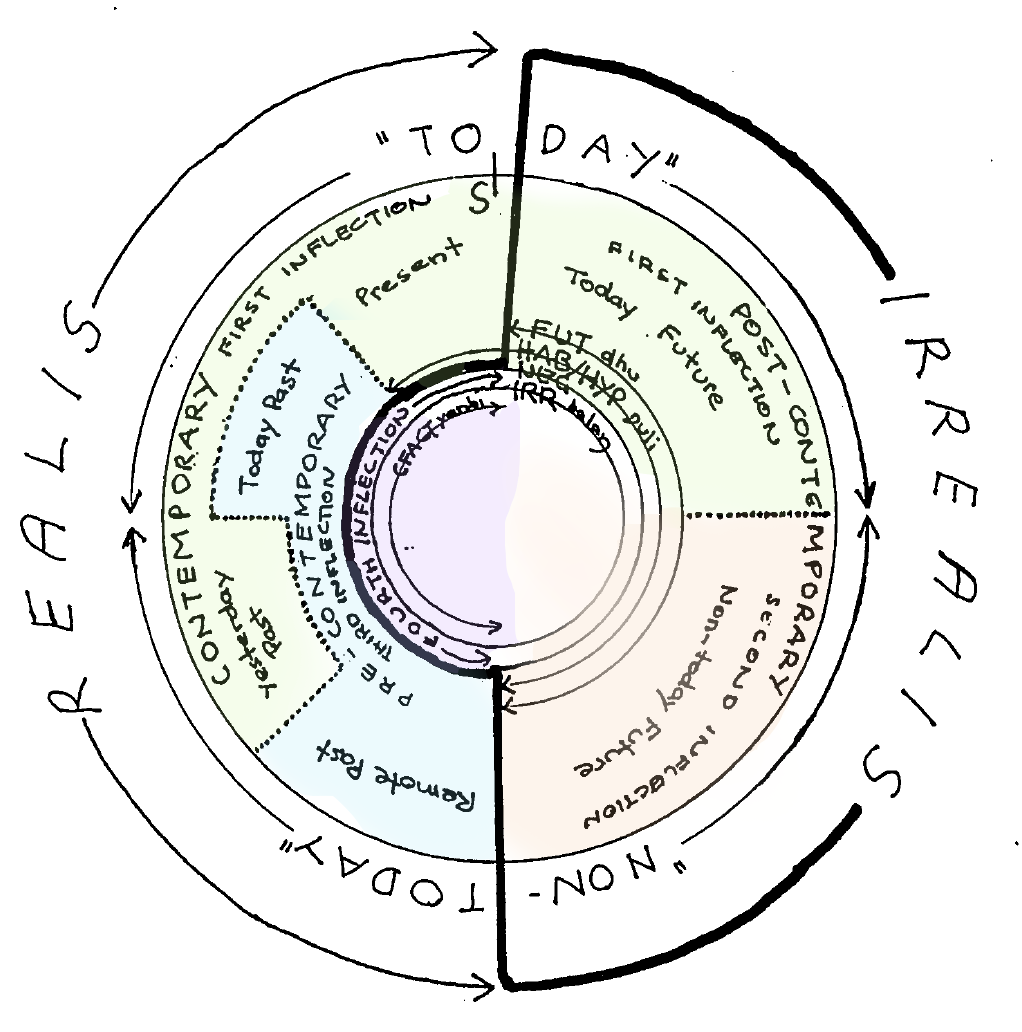
\includegraphics[width=0.85\textwidth]{WilkinsonDiagram362Col}
\end{figure}

Chapter \ref{yol-bkgd} provides background on Yolŋu Matha and the morphology of these languages' verbal paradigms, orienting the discussion around connections between temporal and modal concepts (particularly intention, prediction and futurity) and notions of relative grammatical ``prominence'' of tense, mood and aspect \citep[\textit{cf.}][]{Bhat1999}. %Subsequent chapter(s) focus on a number of morphosemantic phenomena (namely ``cyclic tense'' and ``asymmetric negation'') in the ``Western Dhuwal'' varieties of Yolŋu Matha, in view of providing an account of the semantics of the inflectional categories.



Subsequently, data further demonstrating the the expression of temporomodal distinctions and the interpretive intricacies of WD's paradigm semantics, focussing on a number of morphosemantic phenomena in Western Dhuwal(a) are provided in chapters \ref{sec:djr-temp} and \ref{sec:yol-mood} below. 

In light of these data, in chapter \ref{anY}, I propose a formal treatment of the paradigm on the basis of two semantic features: a temporal one -- \textsc{\textit{non-final instantiation}} -- and a modal one -- \textsc{\textit{metaphysical nonveridicality}}. As we will see, the notion of \textbf{branching times} ---introduced in chapter \ref{IntroCh} and deployed in the analysis of \textit{bambai} (ch. \ref{bambai.semx}) --- permits for a motivated, unified account of the ostensibly disparate sets of usage contexts that license each of \gls{wd}'s four inflectional categories. The essay concludes by considering the landscape of semantic variation across varieties of Yolŋu Matha, suggesting that the \gls{wd} system has arisen as a consequence of reanalysis and contact-induced meaning change.

\chapter{Background}\label{yol-bkgd}

\section{Grammars of TMA: the notion of ``prominence''}

In a \citeyear{Bhat1999} monograph, \citeauthor{Bhat1999} posits a typological parameter along which languages variably assign prominence to \textsc{tense, aspect \textup{or} mood}. For Bhat, determining which of these grammatical macrocategories a given language appears to assign ``prominence'' gives rise to a number of generalisations about characteristics of that language's grammar (``correlatable characteristics''). In particular, he suggests that, in a language where $ \mathcal C $ is given grammatical prominence, notions belonging to the other two categories tend to be ``viewed in terms of $ \mathcal C $'' (7).


An important consequence of this typology, in which languages can be classified and differentiated on the basis of these three broad types, is the implication that languages can ``move between them'' --- that is observable, synchronic variation across this parameter points to a history of reanalysis of, for example, temporal categories as modal ones. While Bhat does not explore this consequence of his typology in detail, he does point to observations in the grammaticalisation literature that have demonstrated ``cross-categorial change'' --- that is, situations where lexical material denoting some temporal, modal or aspectual category come to be reanalysed conveying meaning about a category in another semantic domain. Bhat suggest, for example, that the well-attested alternative grammaticalisation trajectories described by \cite{Bybee1994} (among others) and represented in Figure \ref{ta-gram} are determined by the ``prominence'' that a given language accords to either temporal or aspectual distinctions \citeyearpar[182]{Bhat1999}. Of course, this treatment to some degree begs the question. In a given pair of related languages, what is it that underpins the change from, \textit{e.g.}, perfect marking to perfective marking for $ \mathcal L_1 $ versus past-tense marking in $ \mathcal{L}_2 $?

\begin{figure}[h] \caption{Two examples of attested meaning change between the aspectual and temporal domains}\centering\label{ta-gram}

\begin{subfigure}[t]{.45\textwidth}\centering
		\begin{tikzpicture}[baseline=5pt]
		\draw  (0,0) node(pf)  {\textcolor{forest}{\textsc{perf}}};
		\draw (1.75,.5) node(pv) {\textsc{pfv}};
		\draw (1.75,-.5) node(ps)  {\textcolor{red}{\textsc{pst}}};
		\draw[thick,->] (pf) -- (ps);
		\draw[->] (pf) -- (pv);
	\end{tikzpicture}

\caption{\gls{perf} grams develop into \gls{pfv} markers (\citealp[e.g.][]{Condoravdi2014} for Indo-Aryan) or \gls{pst} markers (\citealp[e.g.][]{Schaden2012} a.o.)}
		\end{subfigure}\hfill
\begin{subfigure}[t]{.45\textwidth}\centering
		\begin{tikzpicture}[baseline=5pt]
		\draw  (0,0) node(pg)  {\textcolor{forest}{\textsc{prog}}};
		\draw (1.75,.5) node(ip) {\textsc{ipfv}};
		\draw (1.75,-.5) node(pr)  {\textcolor{red}{\textsc{pres}}};
		\draw[->] (pg) -- (ip);
		\draw[thick, ->] (pg) -- (pr);
	\end{tikzpicture}\caption{\gls{prog} grams develop into \gls{ipfv} markers (\citealp[see][]{Deo2015a}) or \gls{pres} markers (\citealp[e.g.][]{Heinrichs2002} for Neo-Aramaic)}
		\end{subfigure}
%\begin{tikzpicture}
%	content...
%\end{tikzpicture}
\end{figure}

\subsection{Futurity and mood-prominence}
Bhat marshalls data from Tibeto-Burman to show that ``mood-prominent'' languages have a tendency to grammaticalise a \textsc{future/nonfuture} distinction. He points in particularly to Manipuri ([\gls{mni}] Tibeto-Burman: Manipur), where this tense distinction appears to have ``developed from an earlier realis-irrealis modal distinction'' \citeyearpar[19]{Bhat1999}. Semantic connections between modal and future concepts are further suggested by frequently-attested semantic change pathways between, for example, expressions of intention and obligation (\textit{sc.} bouletic/deontic necessity) and futurity \citep[and then to epistemic modality, \textit{e.g.},][]{Bybee1978,Bybee1991,Bybee1994,Kuteva2019}.\footnote{\citet*{Bybee1991} hypothesise that the ``age'' of a future marker (\textsc{FutAge}) can be assessed in view of its semantic domain. In effect this amounts to a ``pathway'': $\textsc{deontic}\to\textsc{circumstantial}\to\textsc{future}\to\textsc{epistemic}$ \textit{etc.}} In her account of the diachrony (and ``instability'') of future expression in Romance, for example, \citet[31, 75, 106]{Fleischman1982} claims that as future markers become ``more temporalized'' (which she connects to their agglutination), functional pressure to recruit novel modal constructions emerges --- an early conceptualisation of a grammaticalisation cycle/``spiral.''
	%
	%The verbal suffix \textit{-le} is a future tense marker in Manipuri [\gls{mni}], whereas \citet[67ff]{Bhat1999} shows that in related Mao Naga [\gls{nbi}], it encodes irrealis modality, occurring in a number of modal, counterfactual and evidential constructions.
	%
	%\pex\a\begingl\gla \rightcomment{[Mao Naga]}alemono ovo hrü \textbf{le}-\textsc{t}i-e//
	%\glb Alemo pig buy \textbf{\gls{irr}}-\textsc{relevant}//
	%\glft`Alemo wanted to buy a pig (but couldn't as there was no money).'//\endgl
	%\a\begingl\gla pfo ico avuo bu \textbf{le}//
	%\glb he now meal take \textbf{\gls{irr}}//
	%\glft`He must be taking his meal now.'//\endgl
	%\xe


As suggested in \S~\ref{BT-review}, going back to Aristotle, it is well understood that the future has a dually temporal and modal character. That is, the truth of a future predication has frequently been analysed as changing with the passage of time --- that is ```future contingent'' statements can be neither true nor false' \citep[265]{Thomason1970}. Consequently, utterances about the future are often associated with predictive illocutionary force (this was a major theme guiding the analysis in part \textbf{\ref{bambai}}).

Consequently, contemporary formal treatments often embrace a modal semantics for ``future'' operators: one that departs from the earlier, priorian tense logic type approaches where truth is defined relative to time and --- the mirror image of \textsc{past} --- \textsc{future} is a sentential operator that serves to locate their prejacent subsequent to evaluation time.\footnote{Of course, as discussed in \S~\ref{BT-review}, Arthur Prior was crucially concerned about this asymmetry between the future and the past, over the course of his career he departing from an earlier belief in determinism and developing branching time models concerned with the indeterminate nature of the future. (\citealp[see][]{Copeland2020} and also \citealp[13]{Copley2009}).
	
	Generally speaking, on a deterministic view of the future, future morphemes can be unuderstood to universally quantify over an epistemic modal base (``possible candidates for the (preordained) future as far as I'm concerned'', \citealp[\textit{cf.}][]{Giannakidou2018}), whereas on non-deterministic views they quantify over a metaphysical modal base (``possible futures consistent with assumptions about metaphysical facts governing the world.'')} Modal accounts of future, then, often tend to take future-oriented morphology to universally quantify over a modal base. \citet[274]{Thomason1970} proposes a ``supervaluation''-based semantics for future-tensed predication as follows:\footnote{This following Copley's \citeyearpar[14]{Copley2009} conversion of \citeauthor{Thomason1970}'s account based on ``histories'' (which effectively imply sets of historical alternatives) into an equivalent one that speaks in terms of possible worlds. Thomason himself develops $ \mathcal{T\times W} $ frames in a \citeyear{Thomason1984} paper. See also \S\ref{BT-review} and \citep{Stojanovic2014} for discussion and an overview of different semantic approaches to the ``future contingents'' problem.}
\pex $ \denote[w,t]{\textsc{fut }p}=\left\{\begin{gathered}\begin{aligned} 1&\leftrightarrow &&\forall w'\big[w'\approx_t w \to\exists t' [t\prec t' \wedge p(w')(t')]\big]\\
0&\leftrightarrow &&\forall w'\big[w'\approx_t w \to\nexists t' [t\prec t' \wedge p(w')(t')]\big]
\end{aligned}\\
\text{undefined otherwise}\end{gathered}\right.
$\\[.5em]
\textsc{fut} $p$ is true if there's a time $ t' $ in the future of all metaphysical alternatives to $ w $ at $ t $ which $ p $ holds and false if there is no such time.\xe

\noindent As described earlier in this dissertation, $\cap\!\approx_t\!w $ represents the ``historical alternatives to $ w $ at $ t $'' (an equivalence class of worlds with identical histories to $ w $ up to $ t $) --- in effect equivalent to a \textit{metaphysical conversational background} (see \S~\ref{BT-review}.)


 Given how central this metaphysical assumption will be to the analysis, the approach taken by this chapter recasts this possible worlds formalism in terms of branching futures/times models. As in chapter \ref{bambai.semx}'s treatment of the distribution of \textit{bambai}, this will hopefully allow us to perspicaciously cash out the distinctions between the domains of \textsc{real} and \textsc{nonreal} eventualities. That is, a metaphysical conversational background $ \cap\!\approx_i $ will be representable by an equivalence class of branches, undivided until $ i $, that represent metaphysically possible developments of the world from $ i $.

\subsection{Negation and mood}\label{sec:asymneg}

Developing a broad cross-linguistic typology of sentential negation, \citet[208]{Miestamo2005} proposes a class of languages (\textsc{a/nonreal}) which have `grammaticalized the fact that negation belongs to the realm of the non-realized' --- that is, negative and modal operators are shown to interact formally in a number of ways. According to Miestamo, ``asymmetric negation'' phenomena are notably overrepresented in the languages of Australia (and to a lesser extinct New Guinea, driving him to describe \textsc{a/nonreal} as a ``circumpacific phenomenon'' (192, 411)). \citet[\S2.2]{Phillips2021b} provides an overview of a number of mood-based asymmetry phenomena in Australian languages.


For many languages, \textsc{a/nonreal} is manifested as the \textbf{neutralisation} of a grammatical distinction between \textsc{realis} and \textsc{irrealis} modalities in negative clauses. That is, ±\textsc{realised} is associated with a a morphosyntactic distinction in positive clauses that is not available in negative ones. Shown in the Gurrgoni (\gls{gge}, Maningrida: Arnhem) data in (\getref{sn-gvg}), a reality status distinction is morphologically realised in positive clauses (\getref{sn-gvg.rea}-\getref{sn-gvg.irr}) which is not available to its negative counterpart (\getfullref{sn-gvg.neg}), which is obligatorily irrealis-marked and ambiguous between a modal and non-modal reading. As we will see below, a similar phenomenon is exhibited in some varieties of Yolŋu Matha (notably those varieties closer to Maningrida.)


	\pex\deftagex{sn-gvg}
\textbf{Interactions between negation and mood marking in Gurrgoni} 
\iffalse	\a\begingl\glpreamble present-tensed //
\gla dji-na-ni wurrparn//
\glb 3s/3o-see-\textsc{precontemp} emu//
\glft `They didn't see an emu'//\endgl b.\quad\begingl\glpreamble neg present-tensed //
\gla galu dji-na-djirni djit-bolupu nuyu//
\glb \textsc{neg} 3s/3o-see-\textsc{irr} 3s-mother  //
\glft text//\endgl \fi

\a\begingl\glpreamble Past-tensed (nonmodal)\deftaglabel{rea}//
\gla nji-weki-\textbf{ni}//
\glb 2s-talk-\textsc{precontemp}//
\glft `You talked.'//\endgl \a\begingl\glpreamble Past-tensed (modalised)\deftaglabel{irr}//
\gla nji-weki-\textbf{yarni}//
\glb 2s-talk-\textsc{\textbf{irr1}}  //
\glft `You might have talked.'//\endgl	\a\begingl\glpreamble Negative past-tensed\deftaglabel{neg}//
\gla galu nji-weki-\textbf{yarni}//
\glb \textsc{neg} 2s-talk-\textsc{\textbf{irr1}}  //
\glft `You didn't/mightn't have talked.'\trailingcitation{(adapted from \citealp[307]{Green1995})}//\endgl


\xe



Irrealis markers are broadly taken to realise semantic operators which displace the instantiation of a given eventuality into the realm of the nonrealised. Relatedly, negative operators indicate the \textsc{nonrealised} status of some predicate.

Consequently, for languages exhibiting \textsc{a/nonreal}, irrealis and negative operators can be thought of as performing conceptually-related functions. \citep[see also][208]{Miestamo2005}.

 It is on these functional grounds that negation and mood interact; predicting parametric variation across languages.

%todo asymmetry. Muna participates (Bhat 67)


%\subsection{The semantics of a mood-based inflectional system}

\section{Yolŋu Matha}

%Class of YM was discussed in Ch..... 
%To reorient the reader.....
%Djr, Wag are related....
%could move post-defense
Yolŋu Matha is a small language family spoken in North-Eastern Arnhem Land, in the Northern Territory of Australia (map provided in \ref{map}, see also discussion in \S~\ref{sec:ecol}). The family is a subgroup of the larger Pama-Nyungan family, representing something of an enclave in Northern Australia; surrounded by a diversity of unrelated languages.

\begin{figure}[h]
	\centering\caption{Traditional language communities in Northern Australia \citep{Horton1996}.Yolŋu Matha is the gold coloured area within the square in the primary map.\\\textbf{Inset. }Northeast Arnhem land (colourised from \citealt[2]{Wilkinson1991}. Yellow shading indicates the \textit{Yolŋu Wäŋa} (homeland). Brown and green circles indicate the contemporary distribution of Yolŋu languages investigated. Purple circling indicates the neighbouring (but genetically unrelated) Maningrida language family.}	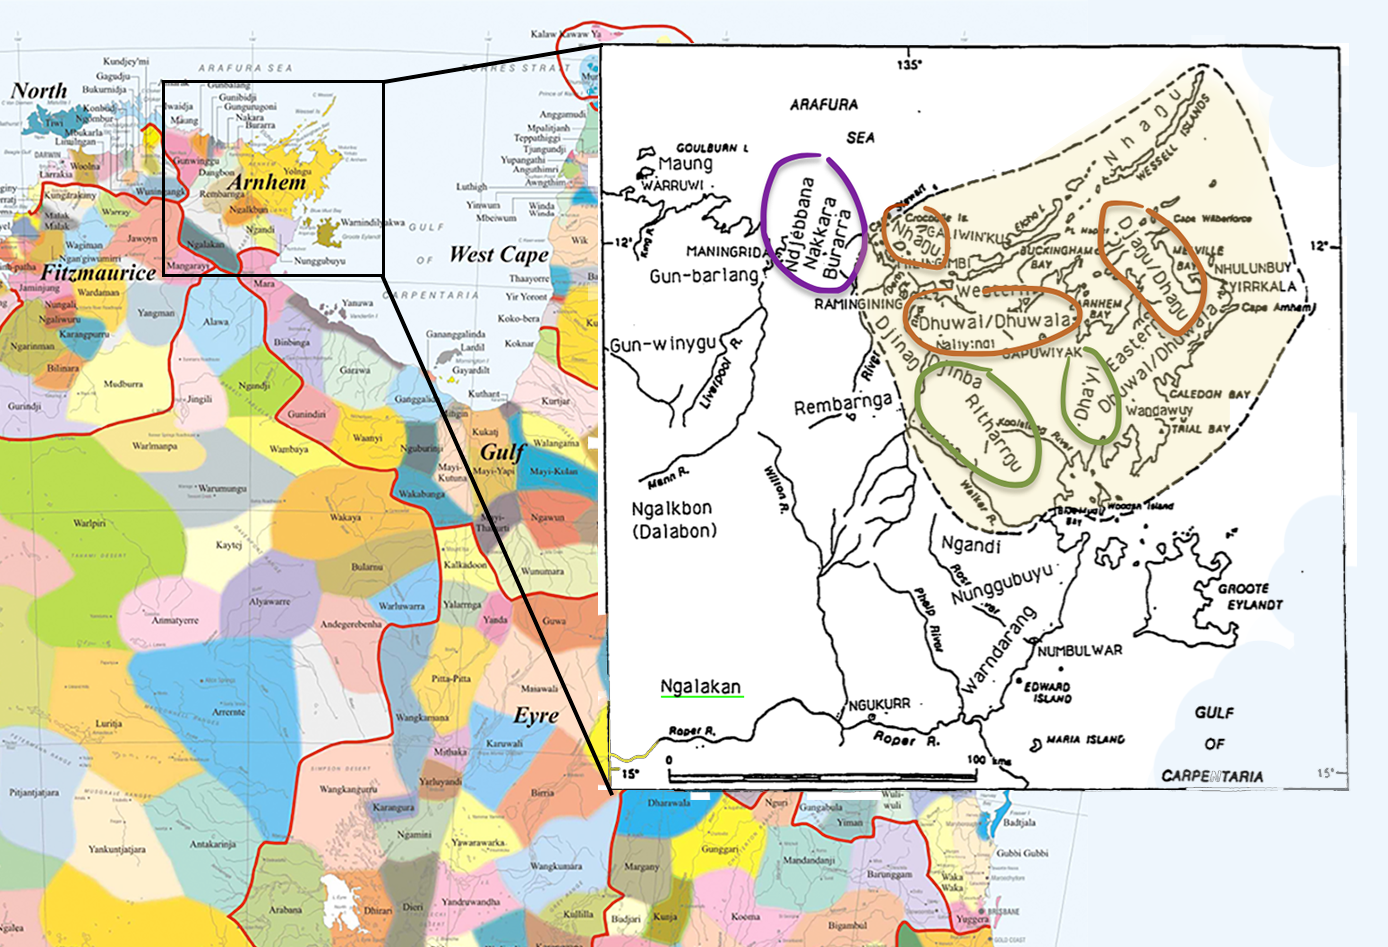
\includegraphics[width=0.9\textwidth]{AustralianLangsCropped.png}\label{map}
\end{figure}


Most Yolŋu linguistic phylogenies posit a high-level split between Western, Northern and Southern subgroups. This is schematised in Figure \ref{YM-phylo}. Yolŋu society is traditionally organised according to a moiety system --- that is, the Yolŋu universe is organised into two ranging sets, \textit{Yirritja} and \textit{Dhuwa} --- and continues to be strictly exogamous with respect to moiety. Given that each Yolŋu clan is associated with a single patrilineal moiety and corresponding language variety, households are necessarily multidialectal, one member of a couple speaking a \textit{Yirritja} lect, the other speaking a \textit{Dhuwa} lect. Children inherit their father's moiety (and language), and marry into their mother's moiety \citep[see also][62\textit{ff}]{Williams1986}. This chapter focuses primarily on a number of Southern Yolŋu varieties (see Fig \ref{DDvars}). 


\begin{figure}
\caption{A broad phylogenetic classification of Yolŋu subgroups, following \citealt{Wilkinson1991,Schebeck2001,Waters1989} a.o.}\centering\label{YM-phylo}
	\begin{tikzpicture}\tikzset{edge from parent/.style=
{draw,
edge from parent path={(\tikzparentnode.south)
-- +(0,-8pt)
-| (\tikzchildnode)}}}
		\Tree  [.\textbf{Yolngu~Matha} [.\textsc{Western} [.Djinang ] Djinba ] [.\textsc{Northern} Nhaŋu Dhaŋu-Djaŋu ] [.\textsc{Southern} \textit{Fig~\ref{DDvars}} ] ]
	\end{tikzpicture}
\end{figure}

\begin{figure}[h]\centering	\caption{Varieties (`clanlects'/dialects) of \textcolor{teal}{Dhuwal}-\textcolor{ochre}{Dhuwala} in the context of the Southern Yolŋu languages \citep[following][13]{Wilkinson1991} with some adaptation following \citet[15]{Schebeck2001}.}\label{DDvars}
	\begin{tikzpicture}[every node/.append style={align=right},every tree node/.style={anchor=north}]
		\Tree [.\textsc{\textbf{Southern~Yolŋu}} [.\textbf{\textcolor{ochre}{Ritharrŋu}-\textcolor{teal}{Wägilak}} $\vdots$ ] [ [.\textbf{Dhay'yi} $\vdots$ ] [.\textbf{Dhuwal-Dhuwala} [.\textsc{western} \node[text=teal,font=\itshape]{\bf\it Djambarrpuyŋu\\Ḻiyagalawumirr\\Ḻiyagawumirr\\Marraŋu\\$ \vdots $}; \node[font=\itshape,text=ochre]{\bf\it Gupapuyŋu\\Wubulkarra\\$ \vdots $}; ]   [.\textsc{eastern} \node[font=\itshape,text=teal] {\textbf{Djapuˀ}\\Marrakulu\\Ḏäṯiwuy\\$ \vdots $}; \node[font=\itshape,text=ochre]{\textbf{Gumatj}\\Maŋgalili\\Munyuku\\Maḏarrpa\\$ \vdots $}; ] ] ] ]
	\end{tikzpicture}
	
\end{figure}\marginnote{right this is the classification in Wilk 91 which follows Dixon 80 presumably? Claire's phylogeny is different in a number of ways. how to handle?}

As indicated in the diagram, the \textit{Dhuwal} and \textit{Dhuwala} groupings effectively represent the distinct clan-lects of a single speech community --- associated with \textit{Dhuwa} and \textit{Yirritja} moieties respectively. Incidentally, \citet{Wilkinson1991} points out that the degree of similarity between Western Dhuwal and Dhuwala are more closely related to one another than either is to Eastern Dhuwal and Dhuwala (I assume that this fact is representable phylogenetically and has been represented in Figure \ref{DDvars}). A (the?) primary distinction between Dhuwal and Dhuwala varieties cross-cutting the language area results from a productive apocope rule (investigated in \citealp{Morphy1977}, \citealp[see also][94\textit{ff}]{Wilkinson1991} for further details.). The formal consequences of Dhuwal apocope on the verbal paradigm are partially indicated in parentheses in Table \ref{djr-pdm-exx} below. The table gives examples of the verb paradigm for each of the major Djambarrpuyŋu conjugation classes as described by \citet[306\textit{ff}]{Wilkinson1991} (parentheses give the corresponding verb group number assigned by \citealt{Lowe1996} for Gupapuyŋu.)


%\section{Dhuwal-Dhuwala: Djambarrpuyŋu \& Gupapuyŋu}\label{djr}
\section{The Yolŋu verb: Typology \& morphosemantics}\label{yol-paradigms}

With the exception of the Western Yolŋu varieties \citetext{\textit{i.e.}, Djinaŋ \& Djinba, see \citealp{Schebeck2001,Waters1989}}, Yolŋu varieties are largely mutually intelligible \citep{Heath1981b,Morphy1983}. Yolŋu languages have a verbal paradigms which are at least partially cognate and likely reconstructable to a proto-system \citetext{\citealp{Schebeck2001}, \citealp[see comparative reconstruction pilot work by ][]{Bowern2009}.} All varieties have between three and six different inflectional classes; each inflection is responsible for encoding (combinations of) temporal (tense/aspect) and modal information --- as described above, it is the semantics of these inflections with which we will be primarily concerned in this dissertation. The forms of each inflection additionally varies depending on the conjugation class associated with a given verb stem (or derivational suffix) --- authors of descriptions of various Yolŋu varieties having identified between three \citetext{\citealp[\textit{e.g.},][]{Waters1989} on Djinba \& Djinba} and nine \citetext{\citealp[\textit{e.g.},][]{Lowe1996} on Gupapuyŋu} distinct conjugation classes.

In view of demonstrating the structure of a Yolŋu verbal paradigm, in this section, I present a brief overview of the morphosemantics of the range of inflectional classes in Wägilak --- the southernmost variety of Yolŋu Matha and a close relative of Dhuwal --- on the basis of new data elicited in the field, in addition to \citeauthor{Heath1980r}'s \citeyearpar{Heath1980r} description of Ritharrŋu.\footnote{Many thanks to Salome Harris for collecting questionnaire-data from Wägilak and Ritharrŋu in Ngukurr, mid-2019.}

\subsection{The Ritharrŋu-Wägilak paradigm}\label{sec:rit.paradigm}

According to \citet[60--75]{Heath1980r}, the Ritharrŋu (Wägilak) verbal paradigm distinguishes six main conjugation classes which, each of which marks four inflectional categories. These inflections establish a three-way tense distinction between the \textcolor{blue}{\textsc{past}}, \textcolor{forest}{\textsc{present}} and \textcolor{ochre}{\textsc{future}}. He describes the fourth category as the \textcolor{purple}{\textsc{past potential}}, supplying data of the latter's use in counterfactual situations. The paradigm is represented by table \ref{rit.paradigm}, while the data in (\ref{wag-infls}) demonstrates the (straightforward) temporal semantics of each of these inflectional categories.


\begin{table}[h]\caption{Examples of conjugation patterns for the Ritharrŋu-Wägilak verbal paradigm \citep[adapted from][63--6]{Heath1980r}}\label{rit.paradigm}\small
	\begin{tabular}{>{\bf}l>{\sc}l>{\it}l>{\it}l>{\it}l>{\it}l}\toprule
		\textsc{class} & \textsc{stem} & \textcolor{forest}{\gls{pres}} & \textcolor{ochre}{\gls{fut}} & \textcolor{blue}{\gls{pst}}\footnotemark & \textcolor{purple}{\gls{cfact}}\\\midrule
		1 & `go' &	wäni & wäni & wäni-\textbf{na}/-\textbf{nya} & wäni-\textbf{ya}\\
 2& `eat' & ḻuka & ḻuk-\gls{I} & ḻuka-\textbf{nha}& ḻuk\textbf{-iya}\\
 3& `chase'& ŋupa& ŋupa-\textbf{ru}&ŋupa-\textbf{na} &ŋupa-\textbf{ra} \\
 4&`hold' & gatha-\textbf{ŋ} &gaṯu-\textbf{lu} &gatha-\textbf{(la)ra} & gatha-\textbf{la} \\
 5&`push' &djaranydju\textbf{-n} &djaranydju\textbf{-ru} &djaranydju\textbf{-na} &djaranydju\textbf{-ra} \\
 6\textsc{b}&`protect' &gunga\textbf{-ma} & gungu\textbf{-ŋu}& gunga\textbf{-wala/-nha} & gunga\textbf{-wa}\\\bottomrule
	\end{tabular}
\end{table}
\footnotetext{Where there are two forms given for the \textcolor{blue}{\gls{pst}} marker, \citet{Heath} is ambivalent about the semantic characteristics of each form --- i.e., whether they are synonymous or whether they represent a defective distinction. We will provide further evidence for the latter persepctive in \S\ref{yol-change}.}



\pex \textbf{The temporal interpretation of each inflectional class in Wägilak}\label{wag-infls}
\a\begingl\gla \rightcomment{\textcolor{forest}{\textbf{[\textsc{present}]}}}\textbf{nhäma} rra yakuthi mukulnha//
\glb see.\textbf{{\I}} 1s now aunt.\textsc{acc}//
\glft`I'm (not) looking at my aunt currently.'\trailingcitation{[RN~20190520]}//\endgl\deftagex{wag-pres}\
\a\begingl\gla \rightcomment{\textcolor{ochre}{\textbf{[\textsc{future}]}}}goḏarrpuy ŋarra \textbf{nhäŋu} mukulnha//
\glb tomorrow 1s see.\II{} aunt.\textsc{acc}//
\glft`I will (not) see my aunt tomorrow.'\trailingcitation{[DW~20190522]}//\deftagex{wag-fut}\endgl
\a\begingl\gla \rightcomment{\textcolor{blue}{\textbf{[\textsc{yesterday past}]}}}ripurru-mirri ŋarra \textbf{nhäwala} mukulnha//
\glb yesterday 1s see.\textbf{\III} aunt.\textsc{acc}//
\glft`I saw (didn't see) my aunt yesterday.'\trailingcitation{[RŊ~20190522]}//\endgl\deftagex{wag-pst}
\xe

\noindent Further, (\getref{rit.mods}) shows the modal uses of \gls{fut} and \gls{cfact} inflections. In (\getfullref{rit.mods.a}-\getref{rit.mods.imp}), \II~is compatible with a number of modal (\textit{e.g.}, deontic, conditional) readings, including in imperative utterances. Similarly, \gls{cfact} is compatible with a range of ``modal-for-the-past''/counterfactual readings, as shown by Heath's translation in (\getfullref{rit.mods.cf}).


\pex \textbf{The \textsc{future} and \textsc{past potential/counterfactual} in modalised contexts in Ritharrŋu-Wägilak}\deftagex{rit.mods}
\a \begingl\gla blijiman ŋay waŋa-na: ``gulu-\textbf{rru} nhe yiŋ'-ŋiri\textdblhyphen{dhi} wäŋa-ya. Yakaŋu nhe \textbf{wäni}-'may garra nhe git lokdap-\textbf{urru}"//
\glb policeman 3s say-\III~ stay-\II~ 2s \gls{dist}-\gls{loc}\textdblhyphen\gls{foc} home-\gls{prom} \gls{neg} 2s go.\II-\gls{neg} \textit{garra} 2s \textit{get} locked.up-\II//
\glft`The policeman said you must stay here at home. Don't go (anywhere) or you'll be locked up.'\trailingcitation{[RŊ~20190520~18']}\deftaglabel{a}//\deftagex{wag-pot}\endgl
\a\begingl\gla \textbf{wäni} nhe//
\glb go.\II~ 2s//
\glft `You can/should/will go.' (or `Go!')\trailingcitation{\citep[104]{Heath1980r}}\deftaglabel{imp}//\endgl
\a\begingl\gla wäni\textbf{-ya} nhe//
\glb go-\V~ 2s//
\glft`You could/should/would/were about to go.'\trailingcitation{\citep[104]{Heath1980r}}\deftaglabel{cf}//\endgl
\xe

This distribution can be straightforwardly represented by appealing to the ``modal trichtomy'' \citetext{\textit{cf.} \citet{VonPrince2019,VonPrincea} --- introduced in \S \ref{vP-trich}, compare (\getref{trichot}), \textit{p.}~\getref{vP-bt0}.} Effectively, Ritharrŋu-Wägilak's four inflections can be thought of as a partition of a branching-time. This is shown in (\nextx) and schematised in Figure \ref{rit-BT}.


\pex \textbf{Domains of the four inflections in Ritharrŋu-Wägilak, given a branching time frame $ \mathfrak U =\langle\mathcal I,\prec\rangle$ and an evaluation index $ i* $}


\denote[i*]{\gls{pres}}  : \textsc{actual present} $ \{i\mid i = i*\} $\\
\denote[i*]{\gls{fut}}  : \textsc{potential} $ \{i\mid i \succ i*\} $\\
\denote[i*]{\gls{pst}}  : \textsc{actual past} $ \{i\mid i \prec i*\} $\\
\denote[i*]{\gls{cfact}}  : \textsc{counterfactual} $ \{i\mid \langle i,i*\rangle\text{ is unordered by }\prec\} $
\xe

\begin{figure}[h]
	\caption{Ritharrŋu-Wägilak's verbal paradigm partitions the branching frame/modal domain (modelled as a set of partially-ordered indices.)}\label{rit-BT}\centering
	\begin{tikzpicture}
		[scale=2.5,level distance=9mm,
		every node/.style={fill=purple,circle,inner sep=1.5pt},
		level 1/.style={nodes=purple,sibling distance=10mm},
		level 2/.style={sibling distance=8mm},
		level 3/.style={sibling distance=4mm},
		level 4/.style={sibling distance=2mm},
		edge from parent/.style={draw,thick}]
		\node[color=blue,minimum size=2mm] {} [grow=right]
		child {node {} edge from parent[densely dotted,color=purple]
			child {node {}
				child {node {}
					child {node {}}
					child {node {}}}
				child {node {}
					child {node {}}
					child {node {}}}}
			child {node {}
				child {node {}
					child {node {}}
					child {node {}}}
				child {node {}
					child {node {}}
					child {node {}}}}}
		child[missing]
		child {node[color=blue,minimum size=2mm] {}
			child {node {} edge from parent[densely dotted,color=purple]
				child {node {}
					child {node {}}
					child {node {}}}
				child {node {}
					child {node {}}
					child {node {}}}}
			child {node[color=purple] {} edge from parent[densely dotted,color=purple]
				child {node {}
					child {node {}}
					child {node {}}}
				child {node {}
					child {node {}}
					child {node {}}}}
			child {node [style={fill=forest,minimum size=4mm},label=above:$ \boldsymbol{{\color{gray!95}i*}} $] {} []
				child {node[fill=ochre] {} edge from parent[densely dashed,color=ochre,every child=every node\.style={fill=ochre,circle,inner sep=1.5pt}]
					child {node[fill=ochre] {}}
					child {node[fill=ochre] {}}} 
				child {node[fill=ochre] {} edge from parent[densely dashed,color=ochre]
					child {node[fill=ochre] {}}
					child {node[fill=ochre] {}}}} };
	\end{tikzpicture}
\end{figure}


As an example then, the contribution of \textcolor{forest}{\gls{pres}} (following standard assumptions about tense) is taken to be the restriction of a given predicate (\textit{P})'s instantiation to actual indices that overlap with the present: \textit{i.e.}, \gls{pres}(\textit{P}) is true iff \textit{P} is instantiated at $ i* $.

\subsection{The central Arnhem linguistic area}
This section has so far sought to familiarise the reader with the basic structure of a Yolŋu Matha verbal paradigm, taking the example of the Ritharrŋu-Wägilak (Southern Yolŋu) variety. 

In the sections that follow, we turn to a description of the distribution of the inflectional categories in Western Dhuwal-Dhuwala (\gls{wd}). As we will see (and as shown in the introduction to this part of the dissertation), there are a number of phenomena that complicate a unified treatment of the semantics of the \textsc{wd} paradigm. Introduced above, these phenomena include a \textsc{cyclic tense} system and \textsc{asymmetric negation}.


Importantly, these phenomena are not exhibited in most Yolŋu lanuages, including those varieties phyletically closest to \textsc{wd}, \textit{viz.} Ritharrŋu-Wägilak as well as the Eastern (\textit{``Miwatj''}) varieties of Dhuwal-Dhuwala centered around Yirrkala (compare figures \ref{YM-phylo} \& \ref{DDvars}.) Similar patterns are, however, characteristic of the languages of Maningrida --- Burarra, Gurrgoni, Nakkara and Ndjébanna. Varieties of Djinaŋ (a Western Yolŋu outlier) are spoken in the Maningrida community and its outstations. The Ramingining community --- traditionally the land of the Ganalbingu tribe (a \textit{Yirritja} Djinba moiety) --- is approximately 100km east of Maningrida. Djinaŋ, Djinba and \gls{wd} (the westernmost varieties of Dhuwal-Dhuwala) all exhibit the cyclicity and asymmetric negation that is characteristic of the grammars of the Maningrida languages.

In view of the sustained contact between the non-Pama-Nyungan Maningrida languages and the (geographically) western varieties of Yolŋu Matha, it is assumed here that these two properties are examples of areal phenomena that characterise the languages of central Arnhem Land \citetext{see appendix 2 of \citealt{Waters1989} for a short investigation of this perspective.}


\begin{center}
	
\huge\sf	 ※
	
\end{center}


\noindent I will argue that these two phenomena --- \textit{cyclic tense} and \textit{asymmetric negation} (w/r/t reality status marking) --- are undergirded by the grammaticalisation of two semantical properties---\textsc{\textbf{non-final instantiation}} and \textsc{\textbf{nonveridicality}} respectively. These properties will be further precised and couched in a more detailed discussion of the expression of temporal and modal categories in \gls{wd} (chh.~\ref{sec:djr-temp}--\ref{sec:yol-mood}). A formal proposal (in terms of branching times) for the semantics of the \gls{wd} verbal paradigm is presented in chapter \ref{anY}.


%todo §§4.1-4 to migrate directly in as descriptive background chapters
\section{Verbal inflection in Western Dhuwal(a)}\label{djr-infl}

%\subsection{\gls{wd} Paradigm structure \& distribution of the inflections}\label{infls}

TMA distinctions in Western Dhuwal(a) are partially encoded in a paradigm that distinguishes four `inflections', which are cognate with a number proto-Yolŋu inflections according to the reconstructions provided by \citet{Bowern2009}. Unlike for Ritharrŋu-Wägilak, summarised above (\S~\ref{yol-paradigms}), work on Dhuwal-Dhuwala varieties---most notably Beulah \citeauthor{Lowe1996}'s notes and lessons on Gupapuyŋu (first published in 1960) and Melanie \citeauthor{Wilkinson1991}'s 1991 Djambarrpuyŋu reference grammar [republished \& cited here as \citealp{Lowe1996,Wilkinson1991} respectively]---has tended to eschew a metalinguistic gloss for these inflections, given the ostensible non-unifiability of their semantics:\footnote{Relatedly, in his treatment of Djinaŋ and Djinba, \citet{Waters1980,Waters1989} glosses the function-in-context of each inflection, perhaps implying a polysemy treatment of each inflection in these languages: ``[In Djinaŋ, t]here are twelve semantic categories for every verb, which are coded by seven suffixal forms. Consequently, five of the forms each code two different semantic categories...'' \citeyear[142]{Waters1980}} the distribution of each of these inflectional categories is discussed in greater detail in this section. In addition to these inflections, the labour of encoding temporal and modal relations in \gls{wd} is shared by a (closed) class of auxiliaries, which appear to interact with the verbal paradigm. 




Further complicating the exposition of this (and a feature across Yolŋu Matha varieties, see \S~\ref{yol-paradigms}), is the fact that there are a number of \textit{conjugation (sub)classes}: \citet{Lowe1996} enumerates nine classes. The (more detailed) description by \citet{Wilkinson1991} shows that these correspond to three larger conjugation classes --- the \textit{Ø-}, \textit{N}- and \textit{Ŋ-}classes --- each associated with a number of subclasses,\footnote{\citeauthor{Wilkinson1991} identifies 14 distinct inflectional patterns in addition to a ``non-inflecting'' class \citeyearpar[307]{Wilkinson1991}.} in addition to ``non-inflecting'' and (semi-)irregular categories \citep{Wilkinson1991}. The paradigm for six \gls{wd} verbs, taken to be representative of distinct different conjugation patterns is given in Table \ref{djr-pdm-exx}.

%todo\mcom{Of course I can provide more detailed information (the subclasses) but that feels like it'd be better appended? The comparative spreadsheet i've made/Claire's 2009 stuff has most of this formative data... \\\textbf{note: Andrea Simms strongly suggests more exposition of the formal paradigm} }
\begin{table}[h]
	\caption{Examples of the paradigm of four morphological TMA inflections in Djambarrpuyŋu [\gls{djr}] and (Gupapuyŋu [\gls{guf}] resyllabification in parentheses).\\{}[\gls{djr}] data and classification from \citet{Wilkinson1991}; [\gls{guf}] data and classification from \textit{Gupapuyŋu} \citeyearpar{Lowe1996}.} \label{djr-pdm-exx}
	\centering
	\begin{tabular}{rl|>{\it}l>{\it}l>{\it}l>{\it}l}
		\textbf{Class} & \textbf{\textit{Example}} & \textup{\I} & \textup{\II} & \textup{\III} & \textup{\IV}\\\midrule
		$\boldsymbol\emptyset_{i}$\hfill(2)& \textit{marrtji} `go' & \textit{marrtji}& \textit{marrtji} & \textit{marrtji\textbf{n(a)}} & \textit{marrtji\textbf{nya}}\\
		
		$ \boldsymbol\emptyset_{\textit{a}} $\hfill (3) & \textit{ḻuka} `consume' & \textit{ḻuk\textbf{a}} & \textit{ḻuk\textbf{i}} & ḻuka\textbf{n(a)} & ḻuka\textbf{nha}\\

		$\boldsymbol\emptyset_{\textit{rr}}$ \hfill (4)& \textit{waṉḏirr(i)} `run' & \textit{waṉḏi\textbf{rr(i)}}& \textit{waṉḏi} & \textit{waṉḏi\textbf{n(a)}} & \textit{waṉḏi\textbf{nya}}\\
		
		
		
		\textbf{N}\hfill(5)& \textit{ḻupthun} `wash' &\textit{ḻuphtu\textbf{n}} & \textit{ḻupthu\textbf{rr(u)}} & \textit{ḻupthu\textbf{rr(una)}} & \textit{ḻupthu\textbf{na}}\\
		
		\textbf{N$ _{L} $}\hfill(6)& \textit{gurrupan} `give' & \textit{gurrup\textbf{an}} & gurrupu\textbf{l(u)}&gurrupa\textbf{ra}& gurrupa\textbf{na} \\
		
		\textbf{Ŋ}\hfill(7)& \textit{nhäma} `see' & \textit{nhä\textbf{ma}} & \textit{nhä\textbf{ŋu}} & \textit{nhä\textbf{ŋal(a)}} & \textit{nhä\textbf{nha}}\\
	\end{tabular}
	
\end{table}


Above, I alluded to Beulah Lowe's eschewal of a ``semantic description'' for each of the four inflectional classes, also followed by Melanie Wilkinson. Throughout, these categories will be glossed with bold-faced Roman numerals, following the conventions established by Lowe (see also Table \ref{Infl-Comparisons-Wilk}, which adapts Wilkinson's summary of glossing decisions made by other grammarians.)% -- complex sentences and predications are investigated in further detail in §\ref{djr-subord}.

%Table \ref{Infl-Comparisons-Wilk}, adapted from \citet[336]{Wilkinson1991} summarises the metalanguage decisions made by other authors in their attempts to describe Dhuwal(a) varieties.

\begin{table}[h]
	\caption{Summary of metalinguistic descriptors deployed by a number of grammarians for the four inflectional classes in a number of Dhuwal/Dhuwala varities, adapted from \citet[336]{Wilkinson1991}.}\label{Infl-Comparisons-Wilk}\small
	\begin{tabular}{lr|llll}
		&&	\textbf{\I}	& \textbf{\II}	&	\textbf{\III}	&	\textbf{\IV}\\\midrule
		\citealt{Wilkinson1991}& \gls{djr} &\textsc{First}&\textsc{Second}&\textsc{Third}&\textsc{Fourth}\\
		\citealt{Lowe1996}\footnotemark &\gls{guf} &Primary&Secondary&Tertiary&Quartenary\\
		\citealt{Tchekhoff1983}& \gls{djr}&\textsc{Bas}e&\textsc{Fut}ure&Past\textsubscript1&Past\textsubscript2\\
		\citealt{Heath1980}& \gls{dwu} & Pres/Fut & Fut/Imp & Past & Past Remote\\
		\citealt{Morphy1983}& \footnotesize Djapuˀ & Unmarked & Potential & Perfective & Past Non-indicative\\
	\end{tabular}
	
\end{table}	\footnotetext{\Citealt{VanderWal1992} adopts the same labelling scheme as \citet{Lowe1996} although her analysis of the distribution of each of Gupapuyŋu's inflectional classes seems to diverge somewhat from \citeauthor{Lowe1996}'s.}

 In the following subsections, I provide examples of the functional domains of each of the four inflections in Western Dhuwal-Dhuwala and other lexical material relevant to encoding TMA relations in this language.

%todo MW diagram is now in the intro to this subpart
% Figure \ref{WilkDia} comprises a (colourised) reproduction of \citeauthor{Wilkinson1991}'s schematisation of the functional domain and collocation features of each Djambarrpuyŋu inflection. Data exemplifying the distribution of WD's four inflectional categories is provided in the subsections below in conjunction with a discussion of the approximate range of each.
%
%\begin{figure}[h]\caption{Melanie Wilkinson's \citeyearpar[326]{Wilkinson1991} schematisation of the complex semantic space associated with each of the four inflectional categories in Djambarrpuyŋu. My colourisation.}\label{WilkDia}\centering
%	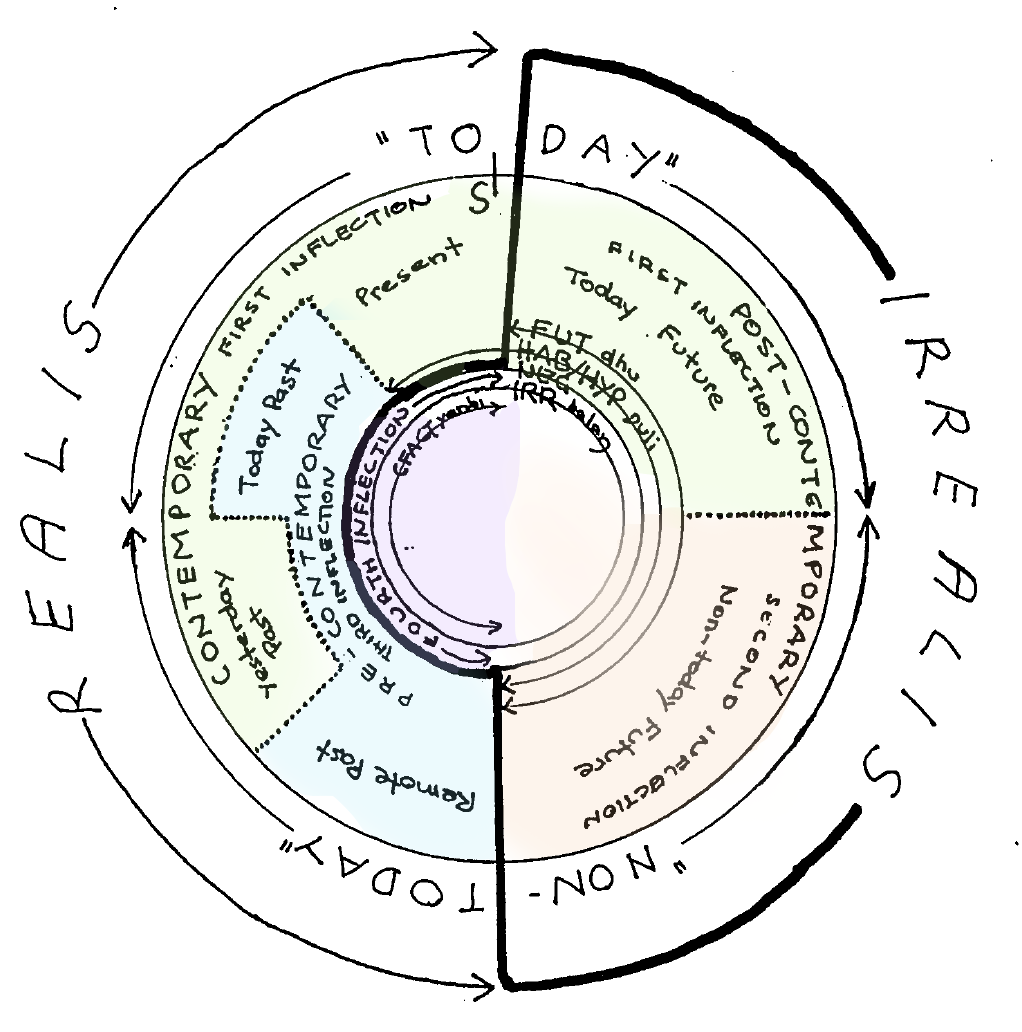
\includegraphics[width=0.8\textwidth]{WilkinsonDiagram362Col}
%\end{figure}

\subsection{The Primary inflection}\label{desc-i}

The `primary' inflection (\I), cognate with inflections in other Yolŋu languages which have been described as ``unmarked'' or ``base'', surfaces in predications that are interpreted with any of \textsc{present}, \textsc{past} or \textsc{future} reference. Here I provide examples of \I-inflected clauses receiving each of these temporal interpretations.

%\mcom{Now for both of these (and i suspect all sentences in this sssection) context ought to be modulable s.t. a non-present reading is available. This can/should/will be tested in the field}
\pex\textit{\textbf{ Present-reference encoded with \gls{I}}}

\a\begingl\deftagex{IPres}\deftaglabel{nhina}
\gla Ŋunhi-y ŋunhi ḏirramu \textbf{nhina} ga//
\glb \gls{texd}\textsc{-erg} \textsc{texd} man sit.\I{} \textsc{ipfv.\I}//
\glft`There that man is sitting.'\trailingcitation{\citep[856]{Tchekhoff1983}}// 
\endgl
%\a\begingl \gla ŋarra \textbf{marrtji}-n dhiyaŋu-n bala//
%\glb 1s go\textbf{.I}-\gls{seq} \gls{prox}.\gls{erg}-\textsc{seq} then//
%\glft`I am going now.'\trailingcitation{\citep[256]{Wilkinson1991}}//\endgl
\a\begingl\gla Ŋarra ga \textbf{ḻuka} gapu (dhiyaŋu bala)//
\glb 1s \textsc{ipfv.\gls{I}} consume.\gls{I} water \gls{texd}.\gls{erg} then//
\glft`I'm drinking water at the moment.'\trailingcitation{[DhG 20190405]}//\endgl
\xe

The sentences given in (\getref{IPres}) show the compatibility between present temporal reference and the \gls{I} inflection: in both cases, the event described by the predicate --- \textit{nhina} `sit.\gls{I}' and \textit{marrtji} `go.\gls{I}' --- is understood as contemporaneous with speech time. In each sentence, imperfective marking (\textit{ga} `\gls{ipfv}') is obligatory in order to establish present reference (see \S \ref{sec:djr-temp}).



In addition to those present-referring sentences in (\getref{IPres}), the data in (\getfullref{pstI}) show compatibility between \gls{I} and past time reference. In each of these examples, the events described by the predicates---\textit{e.g.}, the arrival event described by \textit{ŋayatham} in (\getfullref{pstI.ŋayatham})---\textit{precede} speech time. Similarly, the two past events in (\getref{pstI.rrupiya}) both receive \gls{I} inflection. The instantiation times of both of these events are further restricted (to the recent past) by temporal frame adverbs \textit{barpuru} $\approx$ `yesterday'. % -- frame adverbials of this type are discussed in some detail in §\ref{TFA}.

%\mcom{Is it a shitty idea to use colour coding for more formatting/highlighting options? I want to reserve bold for the verbforms themselves but would like to be able to second-order emphasise non-paradigmatic things like TFAs, aspectual ops...}
\pex\textbf{Past-reference encoded with \gls{I}}\deftagex{pstI}

%\a\deftaglabel{nhama}\begingl\gla barpuru linyu \textbf{nhäma} dirramu-ny//
%\glb yesterday 2d see.\gls{I} boy-\gls{acc}//
%\glft`Yesterday we saw a boy'\trailingcitation{\citep[569]{Tchekhoff1985}}//\endgl

\a\begingl\gla bäru-yi-\textbf{rri} \textbf{barpuru} nhuma-laŋgu rra ŋunhi-li-yi ga ŋäṉḏi-w ŋarra \textbf{barpuru} ḻarr-\textbf{uma} ga nhuma rraku ḻakara-\textbf{ma}\deftaglabel{baru}//
\glb crocodile-\gls{inch}-\gls{I} \textbf{yesterday} 2p-\gls{dat} 1s \gls{texd}-\gls{loc}-\gls{ana} and \gls{mo}-\gls{dat} 1s \textbf{yesterday} search.for-\gls{I} and 2p 1s.\gls{dat} tell-\gls{I}//
\glft`Yesterday, I (appeared) to you as a crocodile there. And I was looking for my mum and you told me (where she was.)'\trailingcitation{\citep[107]{VanderWal1992}}//\endgl

\a\deftaglabel{ŋayatham}\begingl\gla ga \textbf{ŋayatham} ŋunha baṉ'thula-wuy ŋayambalk//
\glb and reach.\gls{I} \gls{dist} \textsc{place}-\gls{assoc} place//
\glft`And (then we) reached the place (associated with) Baṉthula.'\trailingcitation{\citep[461]{Wilkinson1991}}//\endgl



\a\deftaglabel{rrupiya}\begingl\gla ḏirramu-wal yothu-wal bäpa-'mirriŋu-y rrupiya \textbf{barpuru} djuy'yu-\textbf{n} märr \textbf{barpuru} ga \textbf{barpuru} \textbf{buna}-ny dhiyal-nydja//
\glb man-\gls{obl} kid-\gls{obl} father-\gls{kinprop}-\textsc{erg} money \textbf{yesterday} send-\gls{I} \textbf{somewhat} \textbf{yesterday} and \textbf{yesterday} arrive.\gls{I}-\textsc{prom} \gls{prox}.\gls{erg}-\gls{prom}//
\glft`The father sent money to the boy recently and it arrived here yesterday'\trailingcitation{\citep[343]{Wilkinson1991}}//\endgl

\xe


Finally, the examples in (\getref{futI}) below, show the compatibility of \gls{I}-inflected verb forms and \textsc{future} temporal reference.  In these contexts, the presence of \textit{dhu} --- the \textsc{future} marker (to receive a modal semantics) --- is obligatory in order to establish future reference. 

\pex \deftagex{futI} \textit{\textbf{Future-reference encoded with \gls{I}}}
\a\deftaglabel{lakaram}\begingl\gla yalala ŋarra dhu nhokal lakara-\textbf{m}//
\glb later 1s \textsc{fut} 2s\textsc{.obl} tell-\gls{I}//
\glft `Later (today) I'll tell you.' \trailingcitation{\citep[373]{Wilkinson1991}}//\endgl

\a\deftaglabel{buna}\begingl \gla dhiyaŋ~bala walal dhu \textbf{buna}, yalala//
\glb now 3p \textsc{fut} arrive.\gls{I} later//
\glft`They are coming later today.'\trailingcitation{\citep[256]{Wilkinson1991}}//\endgl


\a\begingl\glpreamble \textbf{Deontic force with \textit{dhu}+\gls{I}}//
\gla Way! Nhe dhu gurruka-\textbf{m} helmet! Rom ga \textbf{waŋa}.//
\glb Hey! 2s \gls{fut} wear-\gls{I} \textit{helmet} law \textsc{ipfv.\gls{I}}  say.\gls{I}//
\glft`Oy! You wear a helmet! The law says so!\trailingcitation{[AW~20170730]}//\endgl

%\a\deftaglabel{marrtji}\mcom{Actually, W claims this is ``imminent action'' so we really just have a futurate use of \gls{I} without \textit{dhu} (interesting data point in itself) This can probably move to the section on future marking (either \gls{I} or \textbf{\textit{dhu}})}\begingl\glpreamble `Imminent action' without \textit{dhu}//
%\gla \ljudge{$ ^{\%*} $}ŋarra marrtji-n \textbf{dhiyaŋu}-n \textbf{bala}//
%\glb 1s go-\gls{seq} \textbf{\gls{prox}.\gls{erg}}-\gls{seq} \textbf{\gls{mvtawy}}//
%\glft`I'm going now.'\trailingcitation{\citep[256]{Wilkinson1991}}//\endgl

\xe


\noindent In each of these three sentences, the event described by the predicate is understood to obtain in the \underline{future} of speech time (modulo additional constraints on imminence/immediacy, to be described in the next subsection.)

What we have seen here, then, is that \gls{I} is compatible with temporal reference at, prior to, and subsequent to the moment of speech: on the basis of this evidence, we might conjecture that it has no temporal semantics. %\mcom{Evidence of infelicity of \textit{dhu}-less future readings? I actually kinda doubt on the basis of Tonnhauser, Bohnemeyer's work that this is going to be a hard constraint}
%(Although according to \citet[256]{Wilkinson1991} (\getfullref{futI.marrtji}), a futurate interpretation is ostensibly available. This use is unavailable to Ramingining speakers.

\subsection{The Secondary inflection}\label{desc-ii}

Like \gls{I}, the Secondary inflection (\gls{II}) has a range of uses. It is notably obligatory when predicating of future times \underline{beyond the current day} and is the main strategy for forming \underline{imperative sentences}.

\pex\deftagex{futII} \textbf{\textit{Future-reference encoded with \gls{II}}}
\a\deftaglabel{lakaraŋ}\begingl\glpreamble \textbf{Co-occurring with \textit{dhu} `\gls{fut}'}//
\gla yalala-ŋu-mirri-y ŋula~nhätha ŋarra *(dhu) nhokal lakara\textbf{-ŋ}//
\glb later-\textit{ŋu}-\gls{prop}-\gls{erg} sometime 1s \textsc{fut} 2s-\gls{obl} tell-\gls{II}//
\glft`I'll tell you sometime later on'\trailingcitation{(\citealp[346]{Wilkinson1991}; neg. judg. -- DhG~20190405)}//
\endgl

\a\begingl\glpreamble\textbf{ Infelicity of \gls{I} with non-today future}//
\gla Barpuru goḏarr ŋarra dhu nhä(\textbf{-ŋu/$^\#$-ma})//
\glb funeral tomorrow 1s \gls{fut} see(-\gls{II}/$^\#$-\gls{I})//
\glft `I'll see the funeral tomorrow'\trailingcitation{[AW~20180730]}//\endgl

\a\begingl\glpreamble\textbf{\textit{dhu}+\gls{I} implies same-day future}//
\gla walal $^\#$(dhu) \textbf{buna} yalala//
\glb 3p $^\#$(\gls{fut}) arrive.\gls{I} later//
\glft`They'll arrive later.'\\
\textsc{\textbf{speaker comment:}} You're talking about \textit{yalala}; not tomorrow, sometime today.//\endgl


\xe

\noindent The two sentences in (\getref{futII}) show how \gls{II} is used in concert with the particle \textit{dhu} to establish future temporal reference.
% The conditions on the (non-)appearance of \textsc{fut}-marker \textit{dhu} are unclear at the present time (see §\ref{dhu} for more), but future-readings with \gls{II} do not appear to be reliant on this auxiliary (cf. the data in (\getref{futI}) above).
  A notable contrast between (\getfullref{futI.lakaram}) and (\getfullref{futII.lakaraŋ}) is the apparently obligatory retrieval of a \textsc{today}-reference time for \gls{I}-inflected futures, as against a  \textsc{beyond-today}-reference time for \gls{II}-inflected futures.\footnote{\citet[347]{Wilkinson1991} gives an example of a speaker using a \textit{dhu}-\gls{II} structure in the context of a narrative she is telling, signalling that she `will (return to the time of the old people).' Wilkinson takes this as evidence of an association between \gls{II} and the irrealis. This generalisation is pursued in detail in this chapter.} Effectively, this distinction seems to be one place where the grammar of Dhuwal(a) grammaticalises ``temporal remoteness'' (\citealt{Comrie1985,Dahl1985} referred to elsewhere in the literature as ``metrical tense'' \citealp[\textit{e.g.},][204]{Chung}).\footnote{Although \citet[39]{Heath1980} suggests of the \gls{II} future in Dhuwal Proper (his \textsc{Fut/Imp}) that this form encodes a type of ``normative nuance'' (a clear extention of imperative flavour into future assertions.)}


(\getref{irrII}) shows the compatibility of \gls{II} with a (future-oriented) possibility reading. Modal particles including \textit{balaŋ(u), ŋuli} and \textit{bäynha} are responsible for the `weakening' or `downtowning' of the speaker's commitment to the prejacent proposition. 
%Modal operators are described in §\ref{modals}.

%\mcom{It would be good to get sentences with richer context (i.e. an established time of instantiation for the prejacent (tomorrow, imminently etc...)) 
%	This said we can probably assume that the we're talking about immediate future here... Is \gls{I} incompatible with this? There's not much more to say here until I have speaker judgments on this question.}
\pex\textbf{Future possibilities marked with \gls{II}}
\a\deftagex{irrII}\begingl\gla Ŋarra ŋuli \textbf{bäynha} dhiŋgu-\textbf{ŋ} ŋawulul-yu//
\glb 1s \textsc{hyp} \gls{mod} die-\gls{II} smoke-\textsc{erg}//
\glft`I might die from the smoke.'\trailingcitation{\citep[164]{Buchanan1978}}//\endgl
\a\begingl\gla ŋayi bala \textbf{balaŋu} bukthu-\textbf{rru}//
\glb 3s \gls{mvtawy} \gls{mod} break-\gls{II}//
\glft`It (the recorder) might break.'\trailingcitation{[DhG~20190417]}//\endgl
\xe



\gls{II} is additionally used to encode imperative clauses (\getref{impII}). Shown in (\getfullref{impII.proh}), negative imperatives (probibitives) are treated identically.\footnote{Although, as discussed in Ch. \ref{NEC} (see also \citeauthor{Phillips2021b} ms. `Negation (in Australian Languages)'), the use of privative-marked nominals is another common, more ``indirect'' directive convention.}

\pex\textit{\textbf{Imperative force with \gls{II}}}\deftagex{impII}
%\a\begingl\gla g...y, ḻupmara-\textbf{ŋu}-n ŋarra-ny//
%\glb \textsc{name} wash-\gls{II}-\gls{seq} 1s-\gls{prom}//
%\glft`G...y, wash me!'\trailingcitation{\citep[360]{Wilkinson1991}}//\endgl

\a\begingl\gla wäy! gurtha ŋunha, nhawi, ḏutji män-\textbf{ŋu}, bakmara-\textbf{ŋu}//
\glb hey! fire(wood) \gls{dist} what's.it firesticks get-\gls{II} break\textbf{-II}//
\glft`Hey! Get that firewood, what's it, those firesticks, and break them.'\trailingcitation{\cite[114]{VanderWal1992}}//\endgl

\a\deftaglabel{proh}\begingl\gla yaka walala-ŋ buku-bakamara-\textbf{ŋ}//
\glb \gls{neg} 3p-\gls{dat} head-break-\gls{II}//
\glft `Don't answer them!'\trailingcitation{\citep[360]{Wilkinson1991}}//\endgl


\a\begingl\gla nhä\textbf{-ŋu} nhanŋu dhurrwara!//
\glb look-\gls{II} 2s.\gls{dat} door//
\glft`Look at her mouth!'\trailingcitation[AW 20180731]//\endgl

\xe

Here, \II-marked predicates have been shown to be compatible with \textbf{future} temporal reference. They co-occur with \textit{dhu} (which we analyse as a \textsc{future} particle) to establish instantiation of the predicate subsequently to the day of utterance. \II~also occurs in imperative utterances and in (future-oriented) modal constructions with present perspective (\getref{irrII}).


\subsection{The Tertiary inflection}\label{desc-iii}

The Tertiary inflection (\gls{III}) is generally associated with predications about the \textsc{past}. An important caveat, however, is that this inflection is \ul{infelicitous when describing \textsc{recent} events instantiated \textsc{before the current day}.} The examples in (\nextx) below show the compatibility between \gls{III} and a reference time that is `earlier today. In (\getfullref{pstIII.rp}-\getref{pstIII.sdp}), apparent complementary distribution between \gls{I} and \gls{III} provides evidence of the categoricity of this distribuitional constraint.

\pex \textbf{\textsc{Today past} and the \gls{III} inflection}\deftagex{pstIII}


\a\deftaglabel{gathur}\begingl\gla Gäthur ŋayi \textbf{marrtjin} räli Galiwin'ku-ŋur//
\glb today 3s go.\gls{III} hither \textsc{place}-\gls{abl}//
\glft`[Earlier] today he came from Galiwin'ku.'\trailingcitation{\citep[150]{Buchanan1978}}//\endgl

\a\deftaglabel{bili}\begingl\gla Bili ŋayi \textbf{marrtjin} dhipuŋur natha-ŋur nyan'thuna-ŋur//
\glb \textsc{compl} 3s go.\gls{III} \textsc{prox.abl} food-\gls{abl} eat.\gls{IV}-\textsc{abl}//
\glft`He's already gone from having lunch here.'\trailingcitation{\citep[150]{Buchanan1978}}//\endgl

\a\begingl\gla dhiyaŋu~bili goḏarr'mirri ga-\textbf{na} dhärra-\textbf{na} märrma' malwan, bala ŋayi Ŋarritjnydja wurrth-\textbf{urruna}.//
\glb \gls{prox}.\gls{erg}~\gls{cplv} morning.\gls{prop} \gls{ipfv}-\gls{III} stand-\gls{III} two \textit{sp.~Malvaceae} \gls{mvtawy} 3s \gls{malk}.\gls{prom} pull-\gls{III}//
\glft`Earlier this morning, there were two trees standing [there], then Ŋarritj pulled them up.'\trailingcitation{[DB~20190405]}//\endgl

\a\begingl\glpreamble \textbf{Infelicity of \gls{III} with \textsc{recent past}\deftaglabel{rp}}//
\gla barpuru ŋarra nhä\textbf{(-ma/*-ŋala)} ḏetuŋ//
\glb yesterday 1s see\textbf{(-\gls{I}/$^\#$-\gls{III})} buffalo//
\glft`I saw a buffalo yesterday.'\trailingcitation[MD 20180802]//\endgl

\a\begingl\glpreamble\textbf{ Infelctity of \gls{I} with \textsc{today past}}\deftaglabel{sdp}//
\gla gathura ŋarra nhä\textbf{($^\#$-ma/-ŋala)} ḏetuŋ dhukarra-ŋura//
\glb today 1s see\textbf{$ ^\# $-\gls{I}/\gls{III}} buffalo road-\gls{loc}//
\glft `I saw a buffalo down the road today'\trailingcitation{[MD 20180802]}//
%\textsc{comment.} Event could have happened this morning or ten minutes before speech time.//\
\endgl
\xe

%todo ??unsure what this means?? \mcom{Potentially look for a ref for this or provide data that makes this unambiguous...}
\noindent(\getfullref{pstIII.gathur}) shows the compatibility between temporal frame adverbial (TFA) \textit{gäthur(a)} `today' and \gls{III} in \gls{djr}, which leads to an temporal interpretation of `earlier today.'\footnote{Note however that the reckoning of \gls{tfa} \textit{gäthur(a)} differs to that of English and other familiar languages as shown in (\getfullref{neg-pst.munha}), where \textit{gäthur munhawa} `today nighttime' is interpreted as ``last night'' and still triggers \gls{III} marking on the verb.} However even in the absence of a \gls{TFA}, the event described in (\getref{pstIII.bili}) is interpreted as having been instantiated \textsc{earlier.today}/in the immediate past of speech time. Nonetheless, as the data in (\nextx) show, a description of \gls{III} as `hodiernal/same-day past' tense marker is inadequate.


\pex\textbf{\textsc{Remote past} and the \gls{III} inflection}\deftagex{remIII}

%\a\deftaglabel{wawa}\begingl\gla nhä nho-kiyin-gal wäwa-'mirriŋu-y warkthu-\textbf{rr} ŋäthil rarrandharr-yu//
%\glb what 2s-\textsc{emph}-\gls{obl} bro-\gls{kinprop}-\gls{erg} work-\gls{III} before dry~season-\gls{erg}//
%\glft`What did your brother do last summer?'\trailingcitation{\citep[343]{Wilkinson1991}}//\endgl

\a\begingl\glpreamble\textsc{context.} A dreamtime myth.\deftaglabel{baru}//
\gla bäru ga-\textbf{na} marrtji-\textbf{na} beŋuru Ḏulkarri'garri-ŋuru//
\glb crocodile \gls{ipfv}-\gls{III} go-\gls{III} \gls{indef}.\gls{abl} \textsc{place}-\gls{abl}//
\glft`The crocodiles came from Ḏulkarri'garri.'\trailingcitation{\Citep[111]{VanderWal1992}}//\endgl

\a\deftaglabel{sydney}\begingl\gla (Ŋathili) ŋarra marrtji-\textbf{na} Sydney-lili//
\glb before 1s go-\gls{III} Sydney-\gls{all}//
\glft`I went to Sydney long ago.'\trailingcitation{[DhG~20190504]}//\endgl

\a\deftaglabel{malwan}\begingl\glpreamble\textsc{context.} The speaker is describing a locality as it was in her youth.//
\gla märrma' ga-\textbf{n} malwan-dja dhärra-\textbf{n} yindi maṉḍa-ny//
\glb two \textsc{ipfv}-\gls{III} hibiscus-\gls{prom} stand-\gls{III} big 3d-\gls{prom}//
\glft`Two big hibiscus flowers were (growing).'\trailingcitation{\citep[339]{Wilkinson1991}}//\endgl



%todo heath  dhuwal -- unexpected I --- this is a nice datapoint, but it's unclear and it's also on whatever variety H was working on.

%\a\deftaglabel{wuŋgan}\begingl\glpreamble\textsc{context.} A man is telling a story from long ago . His friend's dog has spotted a water goanna.//
%\gla ...ŋunhi wurkaḏi-y nhä-\textbf{ŋal}-{na} ŋinya dharpa-lil-a ŋal'yu-\textbf{na} nhäwi wan'kawu-ya//
%\glb \gls{texd} \textsc{name}-\gls{erg} see-\gls{III}-\gls{seq} 3s.\gls{acc} tree-\gls{all}-\gls{seq} ascend-\gls{III} whatsit water.goanna-\gls{ana}//
%\glft`\textit{Wukaḏi} watched it scramble up into a tree, the water goanna.'\trailingcitation{\citep[193]{Heath1980}}//\endgl
%todo >>>>> \marginnote{I've taken some liberties with the glossing here, Heath has the second verb \textit{ŋal'yuna} as \gls{I} with a \textsc{seq} marker... to investigate further perhaps}



\xe


Unlike the \textsc{hodiernal} temporal interpretations that the sentences in (\blastx) receive, the sentences in (\lastx) involve reference to the `\textsc{remote past}.' In (\getfullref{remIII.baru}-\getref{remIII.sydney}),%\mcom{may be easier just to get a similar non-interrogative sentence to do what \lastx b does}
 the instantiation time of the predicate is restricted by frame adverbials: \textit{ŋäthil(i)}, which picks out a time `in the distant past; prior to/earlier than (some other time)' \citep[158]{Wilkinson1991}, in addition to and \textit{rarrandharryu} `dry season':\footnote{The suffix \textit{-Thu} (\textit{-yu} as a postsonorant allomorph), glossed here as \gls{erg} is used to mark ergative NPs as well as instrumental (\gls{instr}) NPs and to form TFAs out of nominals \gls{temp}.} The cooccurrence of these expressions restricts the predicate being questioned to \textit{a prior dry season}. Conversely, the declarative sentence in (\getfullref{remIII.malwan}) requires no adverbial specification. A \textsc{remote past} interpretation arises as a result of the \gls{III} inflection alone, which is precised pragmatically by the discourse context (\textit{sc.} a narrative that the speaker is telling about her childhood.) (\getref{remIII.malwan}) will be able to retrieve a same-day past interpretation as well, with sufficient contextual support.

%\mcom{This discussion of the Maningrida treatments of ``frame'' and ``tense'' may be better placed • entirely in the lit. review, • after the general data discussion of inflections, or • in the following chapter.} 
The ostensible `discontinuity' of the times that predicates receiving \gls{I} and \gls{III} inflection can refer to has been described in preceding literature as \textbf{\textsc{cyclic time reference}} \citep[88]{Comrie1983}. In her treatment of Burarra [\gls{bvr}], \citet{Glasgow1964} draws a distinction between `tense' and `frame of reference' (`timescale' for \citealt[48]{Green1987}). These, in effect, amount to categorical interpretive interactions between morphological marking and sets of contexts. The interaction between these can be understood as giving rise to a reference interval. This style of analysis has been adopted and developed by others working on Maningrida languages \citetext{\citealt[165]{Eather2011} for Nakkara [\gls{nck}], \citet{Green1995} for Gurr-goni [\gls{gge}] and \citet{McKay2000} for Ndjébanna [\gls{djj}].} The interpretation of interacting ``tense'' morphology and reference frames is schematised in Table \ref{GlaswegianTR}. 
%todo The following chapter further treats and formalises this analysis.



\begin{table}[h]\centering\onehalfspacing
		\caption{A \citealt{Glasgow1964}-style analysis of \textbf{past-time restrictions} introduced by the verbal inflections, adapted for the Dhuwal(a) data. \gls{I} and \gls{III} inflections correspond to Eather's \textbf{contemporary} and \textbf{precontemporary} ``tenses'' (``precontemporary'' is Eather's \citeyearpar[166]{Eather2011} relabelling of Glasgow's ``remote'' tense.)}\label{GlaswegianTR}
	\begin{tabular}{@{}llll@{}}\toprule
		
		&                 & \multicolumn{2}{c}{\textsc{frame}}          \\ 
		&                 & \multicolumn{1}{c}{\textbf{today}}         & \multicolumn{1}{c}{\textbf{before today}}      \\\midrule
		\multirow{2}{*}{\textsc{\rotatebox[origin=c]{90}{infl}}} & \textbf{\phantom{\gls{I}}\gls{I}}    & now           & yesterday/recently \\
		& \gls{III} & earlier today & long ago           \\ \bottomrule%(l){2-4} 
	\end{tabular}
\end{table}


Additionally, there exists a set of psychological predicates that are frequently translated into English as present-tensed stative verbs which also (obligatorily) appear with \textbf{III}. Examples are given in (\nextx).


\pex\deftagex{psychPreds}\textbf{Apparent present reference with \gls{III}}\a\begingl\gla ŋarra dhuwal/dhika djawaryu-\textbf{rr}/rerrikthu-\textbf{rr}/djanŋarrthi-\textbf{n}//
\glb 1s \textsc{prox/indefp} be.tired-\gls{III}/be.sick-\gls{III}/be.hungry-\gls{III}//
\glft`I'm (a bit) tired/sick/hungry'\trailingcitation{\citep[278]{Wilkinson1991}}//\endgl
\a\begingl\gla bili djawar'yu-\textbf{rr}-a//
\glb \gls{cplv} be.tired-\gls{III}//
\glft`They're already tired'\trailingcitation{\citep[365]{Wilkinson1991}}//\endgl
%todo \mcom{Needs elicitation work, appears to be a today-past thing? Are these predicates available with TFAs \textit{barpuru?}, with \textit{ga}? And the other inflections??\\	Test entailments also: \textit{??I was tired this morning but i'm not now??}}
\a\deftaglabel{nhaŋal}\begingl\gla ŋarra dhu dhuwal lakara-m ƞunhi nhä ŋarra nhä-\textbf{ŋal} dhiyaŋ bala//
\glb 1s \gls{fut} \gls{prox} tell-\gls{I} \gls{texd} what 1s see-\gls{III} \gls{prox}.\gls{erg} \gls{mvtawy}//
\glft`I'll tell you what I see right now.'\trailingcitation{\citep[366]{Wilkinson1991}}//\endgl
\xe


\noindent \citet[365--6]{Wilkinson1991} observes that the use of \gls{III} here ``appears to invoke a general temporariness to the state'', noting that the state is ````achieved'' and current relative to the moment of speech.'' That is, the (ostensibly stative) predicates themselves in fact denote state \textit{changes.} This observation is cashed out in \S~\ref{sec:djr-prs}.

%\mcom{Also the get sick/psych/phys condition verbs, some examples also in Buchanan:168}

%todo %%%%%% this is on psych verbs / stative verbs and lexical aspect.
%Additionally, a set of psychological predicates that are frequently translated into English as present-tensed stative verbs appear with \gls{III}. Examples are given in (\nextx).
%
%
%\pex\deftagex{psychPreds}\a\begingl\gla ŋarra dhuwal/dhika djawaryu-\textbf{rr}/rerrikthu-\textbf{rr}/djanŋarrthi-\textbf{n}//
%\glb 1s \textsc{prox/indefp} be.tired-\gls{III}/be.sick-\gls{III}/be.hungry-\gls{III}//
%\glft`I'm (a bit) tired/sick/hungry'\trailingcitation{\citep[278]{Wilkinson1991}}//\endgl
%\a\begingl\gla bili djawar'yu-\textbf{rr}-a//
%\glb \gls{cplv} be.tired-\gls{III}//
%\glft`They're already tired'\trailingcitation{\citep[365]{Wilkinson1991}}//\endgl
%\mcom{Needs elicitation work, appears to be a today-past thing? Are these predicates available with TFAs \textit{barpuru?}, with \textit{ga}? And the other inflections??\\
%	Test entailments also: \textit{??I was tired this morning but i'm not now??}}
%\a\deftaglabel{nhaŋal}\begingl\gla ŋarra dhu dhuwal lakara-m ƞunhi nhä ŋarra nhä-\textbf{ŋal} dhiyaŋ bala//
%\glb 1s \gls{fut} \gls{prox} tell-\gls{I} \gls{texd} what 1s see-\gls{III} \gls{prox}.\gls{erg} \gls{mvtawy}//
%\glft`I'll tell you what I see right now.'\trailingcitation{\citep{Wilkinson1991}}//\endgl
%\xe
%
%\citet[365-6]{Wilkinson1991}, in effect, suggests that the frequent exponence of \gls{III} in these predicates of ``emotional and bodily states'' is a function of their lexical semantics. Unlike their English translations, with \gls{III}, these predicates can be understood as `achievements' (to borrow from Vendler's Aktionsart taxonomy). In these cases then, \gls{III} is licensed because \textit{djarwaryu\textbf{rr(u)}} refers to a state-change before speech time. Consequently, the licensing of \gls{III} in (\getfullref{psychPreds.nhaŋal}) above is a consequence of a completed \textit{seeing} eventuality immediately prior to the \textit{telling}-event described in the matrix clause. This phenomenon is investigated in detail in §\ref{anY}\texttt{.1?} below.


\subsection{The Quaternary inflection}\label{desc-iv}


%\mcom{Is this XLinguistic note worth anything? If so a couple more examples would be nice.}
The Quaternary inflection (\gls{IV}) has a broad range of uses in Dhuwal(a) varieties that correspond in part to categories described in Australian languages including \textit{past potentialis} \citep{Heath1980a}, \textit{past counterfactual} \cite{McKay2011}, \textit{[past] irrealis} \citep[159]{Austin1998} \textit{etc.} It co-occurs with modal auxiliaries (especially \textit{ŋuli} `\gls{hab}' and \textit{balaŋ(u)} `\gls{irr}') in order to describe past habituals (\getref{habIV}) and hypothetical/counterfactual descriptions as in (\getref{hypIV}).


\pex\textbf{\gls{IV} in \textsc{past habitual} predications}\a\deftagex{habIV}\begingl\gla Ŋayi \textbf{ŋuli} märra-\textbf{nha} ŋunhi meṉḏuŋ-nha//
\glb 3s \gls{hab} get-\gls{IV} \gls{texd} snail-\gls{acc}//
\glft`She would (used to) get (collect) snails'\trailingcitation{\citep[147]{Buchanan1978}}//\endgl

%todo \mcom{check ft for (b)} <<<<——— nusure what this note wouldve been about.
\a\begingl\gla ...ŋorra-\textbf{nha} walal \textbf{ŋuli} marrtji-\textbf{nya} ŋunhi-li-yi, + galku-\textbf{na} walal \textbf{ŋuli} ga-\textbf{nha} gapuw wirwiryu-\textbf{na}+ra-w//
\glb lie-\gls{IV} 3p \textsc{hab} go-\gls{IV} \textsc{texd}-\gls{loc}-\gls{ana} wait-\gls{IV} 3p \textsc{hab} \textsc{ipfv}-\gls{IV} water-\gls{dat} turn-\gls{nmlzr}-\gls{dat}//
\glft`They would be lying there, they would be waiting for the water to stir.'\trailingcitation{\citepalias[Djon 5:4]{DB}}//\endgl
\a\begingl\gla waṯuy \textbf{balaŋu} ḻuka-\textbf{nha} chocolate//
\glb dog.\gls{erg} \gls{mod} eat-\gls{IV} chocolate//
\glft`The dog could've/must've eaten the chocolate.'\trailingcitation{[DhG~20190413]}//\endgl

\xe

\pex\textbf{Past modal (counterfactual) predications with \gls{IV} marking}\a\begingl\glpreamble\deftagex{hypIV}\textsc{context.} Speaker had a toothache.//
\gla barpuru balaŋ ŋarra bala dentist-kal marrtji-\textbf{nya} dhiyak//
\glb yesterday \textsc{mod} 1s \gls{mvtawy} dentist-\gls{obl} go-\gls{IV} \gls{prox}-\gls{dat}//
\glft`Yesterday I should have gone to the dentist for a filling'\trailingcitation{\citep[353]{Wilkinson1991}}//\endgl

\a\begingl\gla Yaka balaŋ nhe marrtji-\textbf{nya} Darwin-lil//
\glb \gls{neg} \textsc{mod} 2s go-\gls{IV} Darwin-\gls{all}//
\glft`You should not go to Darwin.'\trailingcitation{\citep[164]{Buchanan1978}}//\endgl


\a\begingl\gla Walanydja balaŋ ŋarraku ḻukuny gulk'mara-\textbf{nha}...//
\glb 3p.\gls{prom} \gls{mod} 1s.\gls{dat} foot.\gls{prom} cut.\gls{caus}-\gls{IV}//
\glft `They were going to/would have cut off his foot...'\trailingcitation{[AW~20190422]}//
\endgl\xe


These data demonstrate the relationship between the \gls{IV} inflection and combinations of past temporal reference and various modal/aspectual operators which encode varieties of ``non-actual'' reality status.\footnote{\textit{N.b.} that, in addition to these inflectional functions, \gls{IV} (and related forms) are additionally used in to derive nominals from verbal predicates (\textit{i.e.}, `\gls{nmlzr}'.) Throughout this part of the dissertation, both inflectional and nominaliser functions of this suffix will be invariably glossed as \gls{IV} (although I am not necessarily committed at this stage to a monosemy account of \textit{these} distributions and a precise semantics for derivational uses of \gls{IV} is not further considered here.)}

So far, we have only considered ``positive'' clauses. Below---in \S\ref{sec:yol-mood}---we see how the picture of WD inflection we have developed here complexifies significantly under negation.


\subsection{Summary}

As mentioned above, a number of authors have eschewed assigning a metalinguistic label to the four inflectional categories that are realised on Western Dhuwal verbs. This is due to the data's apparent resistance to an analysis where each marker realises some unified semantic category (\textit{i.e.}, \textsc{past, present} etc.) It is a contention of the current work that: • this difficulty is due to the interplay of \textsc{cyclic tense} and the \textsc{negative asymmetry} in reality status marking, and • each inflection class can be understood as encoding the status of a predicate with respect to two semantic properties. More detail about these phenomena and their implications for WD verbal semantics are provided below --- \S~\ref{sec:djr-temp} describing temporal expression and \S~\ref{sec:yol-mood} describing modal expression. 

\citeauthor{Wilkinson1991}'s diagramatic representation \citeyearpar[326]{Wilkinson1991} of the relevant distributional features and how they are partitioned by the inflectional system is reproduced as Figure \ref{WilkDia} (\textit{p. \pageref{WilkDia}} above). A compositional analysis for the inflectional classes is proposed in Ch. \ref{anY}.


\chapter{Temporal interpretation \& \textsc{cyclic tense\\{\large distinguishing \I~from \III}}}\label{sec:djr-temp}

\noindent In §~\ref{djr-infl}, I provided a description of the distributional facts of the four `inflectional classes' of Dhuwal(a). As we saw, these inflections are in a paradigmatic relation; all finite verbs receive exactly one inflection.\footnote{The formal identity of some inflections in particular conjugation classes notwithstanding. \textit{marrtji} for example is taken to be formally ambiguous between `go.\gls{I}' and `go.\gls{II}'. Similarly, the ``non-inflecting'' class consisting of 15 borrowed items (\textit{e.g.} \textit{djäma} `work', \textit{riŋimap} `ring up', see \citealp[308]{Wilkinson1991}) will be taken to be defective verb stems, ambiguous between all four inflected forms.} In the Western Dhuwal(a) varieties (as in other Yolŋu languages) verbal inflections play a central role in temporal expression. This chapter will be primarily concerned with understanding the expression of temporal categories in WD, and in particular the semantic properties that distinguish between the licensing of \gls{I} and \gls{III}.

The basic function of inflections \gls{I} and \gls{III} in determining the temporal location of a predicate, for example, is shown in (\nextx).

%todo \mcom{These examples are constructed: need to be checked}
\pex\deftagex{minpair}\textbf{Temporal contributions of \gls{I} and \gls{III}}\a\deftaglabel{minpair}\begingl\glpreamble \textsc{Present temporal reference} with \gls{I}//
\gla gäthura ŋarra \textbf{ga} nhina-$\boldsymbol\varnothing$ wäŋaŋura//
\glb today 1s \gls{ipfv}-\gls{I} sit.\gls{I} home.\gls{loc}//
\glft`I am staying at home today.'//
\endgl
\a\deftaglabel{pst}\begingl\glpreamble\textsc{Past temporal reference} with \gls{III}//
\gla gäthura ŋarra ga-\textbf{na} nhina-\textbf{na} wäŋaŋura//
\glb today 1s \gls{ipfv}-\gls{III} sit-\gls{III} home.\gls{loc}//
\glft`I was sitting at home (earlier) today.'//
\endgl
\xe

The data in (\getref{minpair}) suggest \textit{prima facie} a \textsc{present-past} distinction encoded by \gls{I} and \gls{III} respectively (which, as we saw in the discussion of Ritharrŋu-Wägilak in \S~\ref{yol-paradigms}, is a reasonable analysis for the cognate paradigm in Yolŋu varieties.) However, as discussed in \S~\ref{djr-infl}, data of the type shown in (\nextx) quickly throw up problems for a straightforward account of these inflections as tense markers.

\pex \textbf{Temporal contributions of \gls{I} and \gls{III} (non-today frame)}
\a\deftagex{MetPst}\deftaglabel{I}\begingl\glpreamble\textsc{Recent past} with \gls{I}//
%\gla yo barpuru-ny ŋarra \textbf{marrtji}(*-na) shop-lil//
%\glb yes, yesterday{\sc-prom} 1s go-\textbf{I/*III} shop-{\sc all}//
%\glft`Yes, I went to the store yesterday.'//\endgl
\gla Ŋarra ḻuk-\textbf{a} mänha barpuru//
\glb 1s drink-\gls{I} water yesterday//
\glft`I drank water yesterday.'\trailingcitation{[BM~20190405]}//\endgl
\a\deftaglabel{III}\begingl\glpreamble\textsc{Remote past} with \gls{III}//
%\gla yo ŋarra marrtji-\textbf{na} ŋunhawala ŋäthil baman'//
%\glb yes 1s go-\gls{III} \gls{dist}.\gls{all} before long.ago//
%\glft`Yes, I went there long ago.'//
\gla Ŋunhi ŋarra yothu yäna, ŋarra marrtji-\textbf{na} Sydney-lili//
\glb \gls{texd} 1s child only, 1s go-\gls{III} Sydney-\gls{all}//
\glft`When I was a kid, I went to Sydney.'\trailingcitation{[BM~20190405]}//
\endgl
\xe


The data in (\getref{MetPst}) show that a \textit{temporal remoteness} (or a \textit{``metrical/graded tense''}) distinction is manifested in WD.\footnote{See \citet[Ch. 4]{Comrie1985} for an overview of temporal remoteness systems. Cross-linguistic data on temporal remoteness mechanisms are the subject of recent work including \citealt{Klecha2016,Cable2013,Bohnemeyer2018,Martin2010,Hayashi2015} a.o.} Inflection of predicates with \gls{III} encodes some notion of ``remoteness'', grammatically partitioning the past domain by locating the relevant eventuality at some point in the (subjectively) distant/remote past.


When integrating the data in (\getref{minpair}) and (\getref{MetPst}), and on the (natural) assumption of a model where moments/intervals of time are linearly ordered (\textit{cf.} \S~\ref{LitRev}), the intervals to which \gls{I}- and \gls{III}-inflected predicates can refer are \textsc{discontinuous.} Figure \ref{TempSchem} schematises this discontinuity.


\begin{figure}[h]\caption{Past-time temporal expression in the Yolŋu Matha varieties of Central Arnhem, demonstrating two descriptive phenomena: (a) cyclicity --- the interspersion/discontinuity of \gls{I} and \gls{III} forms and (b) metricality --- the (subjective) division of the past domain between these two forms.\\$\lfloor{\sl today}\rfloor$ indicates the boundaries of the day of utterance. $\boldsymbol{t*}$ is utterance time.}\label{TempSchem}\centering
	\begin{tikzpicture}[scale=1.1]
		% draw horizontal line   
		\draw[<->, line width=.5mm] (0,0) -- (12,0);
		%		\draw[<-, line width=.5mm] (0,0) -- (9.5,0);	
		%draw rex
		\shade[left color=blue!15!white, right color=green!15!white] (0,0.02) rectangle (4.8,1.5);
		%	\fill[green!10!white] (2.5,0.02) rectangle (4.8,1.5);
		\fill[blue!10!white] (4.8,0.02) rectangle (6.8,1.5);
		\fill[green!10!white] (6.8,0.02) rectangle (9.5,1.5);
		\fill[orange!10!white] (9.5,0.02) rectangle (12,1.5);
		
		% draw nodes
		\draw (1.25,0) node[below=3pt] {\textbf{}} node[above=10pt] {\textsc{\gls{III}}};
		\draw (3.675,0) node[below=3pt] {\textbf{}} node[above=10pt] {\gls{I}};
		\draw (5,0)   node[circle,fill,label={below,align=left}:$\big\lfloor{\sl today}$] {} node[below=3pt] {\textbf{}} node[above=3pt] {};
		\draw (6.8,0) node[diamond,shade,outer color=black, inner color  = ochre,label=below:$\boldsymbol{t*}$] {} node[below=3pt] {\textbf{}} node[above=3pt] {\textsc{}};
		\draw (5.8,0) node[below=3pt] {\textbf{}} node[above=10pt] {\textsc{\gls{III}}};	
		\draw (8.15,0) node[below=3pt] {\textbf{}} node[above=10pt] {\textsc{\gls{I}}};	
		\draw (10.75,0) node[below=3pt] {\textbf{}} node[above=10pt] {\textsc{\gls{II}}};	
		\draw (9.5,0)   node[circle,fill,label=below:${\sl today}\big\rfloor$] {} node[below=3pt] {\textbf{}} node[above=3pt] {};
		
		
		%%%braces
		
		\draw [decorate,decoration={brace,amplitude=4pt},xshift=-0pt,yshift=35pt]
		(0.5,0.5) -- (4.5,0.5) node [black,midway,yshift=0.35cm] 
		{\footnotesize metricality};
		
		\draw [decorate,decoration={brace,amplitude=4pt},xshift=-0pt,yshift=40pt]
		(3.5,0.5) -- (9,0.5) node [black,midway,yshift=0.35cm] 
		{\footnotesize cyclicity};
		
	\end{tikzpicture}
\end{figure} 


As described in \S \ref{desc-iii}, previous accounts of this phenomenon have described the data in terms of the oppositions between two binary categories: \textbf{(a)} ``contemporary'' (\gls{I}) vs. ``precontemporary'' (\gls{III}) \textit{tense} marking and \textbf{(b)} a contextually-provided \textsc{today}'' and \textsc{non-today} reference frame. This inflection-reference~frame interaction was shown in Table  \ref{GlaswegianTR} (\textit{p.} \pageref{GlaswegianTR}); each cell of which is represented by one of the datapoints in (\getref{minpair}--\getref{MetPst}). This schema---originally due to  \citet{Glasgow1964} for Burarra data [\gls{bvr}]---has been adopted and adapted by numerous other authors for describing the distribution of verbal inflections in Maningrida languages \citetext{see \citep{Eather2011,Green1987,Green1995} for Nakkara [\gls{nck}], Burarra [\gls{bvr}] and Gurrgoni [\gls{gge}] respectively.}


While \citet[89]{Comrie1985} recommends `appeal to its rarity as an excuse for according it [cyclic tense] marginal status in the theory', the current work contends that we should be desirous of a ``unified'' semantics for each of the verbal inflections.


The following sections consider the status of the \gls{wd} verbal inflections and the relation that they bear to temporal expression. In \S~\ref{sec:djr-prs}, I consider the expression of present reference and imperfectivity in \gls{wd} and how these properties interact with a number of features of the lexical semantics of \gls{wd} verbal predicates (\textit{Aktionsart}). In \S~\ref{sec:djr-pst}, we discuss past predication as it relates to temporal remoteness. Both of these sections provide details relevant to motivating a cyclic tense analysis of the \gls{wd} verbal paradigm.

 \S~\ref{sec:cyc} comprises a discussion of cyclic tense and proposes the relevance of \textsc{nonfinal instantiation} in establishing temporal reference in \gls{wd}.



\section{Aspectuality \& the \gls{wd} verb stem}%\mcom{This section needs to go somewhere --- specific arguments against an ``aspect-based system'' being at the core of the temporal expression in djr. It's less clear that this is the place.}
\label{sec:djr-prs}




\begin{quote}\small
	[T]he present is like the window of a railway carriage in which we are sitting. If it were an infinitesimal slit we could not see out properly, and we could not see the countryside laid out with its features in their proper relations; but since it has a width light can enter and we can see each thing in relation to the next and so form for ourselves a picture of the whole...\hfill{\citep[325]{Hamblin1972}}
\end{quote}



\noindent The obligatory occurrence of \textit{ga} `\gls{ipfv}.\gls{I}' with present-tensed event descriptions has led some authors \citep[\textit{e.g.},][46]{Heath1980} to describe this item as a present-tense marker.\footnote{Compare with Table \ref{Infl-Comparisons-Wilk}. Note that Heath suggests that `the [temporal] value of [\gls{I} and \gls{II}] depends on context, including the presence of particles. He does not attempt a compositional analysis of the verbal inflections \citeyearpar[38,46]{Heath1980}. Additionally, in various texts \textit{ga} (similarly to \textit{gan}) is glossed as a \textsc{dur}ative marker. He does, however, suggest that in various dialects of Dhuwal (particularly Djapu', the variety that seems to diverge more from the Western Dhuwal(a)) that marking this category is uncommon (and in fact the auxiliary may be inflection-invariant.)
	
	While in this Dhuwal sketch, Heath reports working with Djambarrpuyŋu and Djapu' speakers, he also indicates having conducted this work in communities including Ngukurr and Numbulwar (the far south-eastern extent of \textit{Yolŋu wäŋa}.) Consequently, it is plausible that his description is more representative of Eastern Dhuwal (\textit{Miwatj}) varieties than of \gls{wd}.} As we will see here, this is not the most parsimonious analysis of the Dhuwal-Dhuwala inflectional system. The categorical appearance of \textit{ga} (or, in fact, other aspect morphology) is, I will argue, an epiphenomenon of to the well-understood incompatibility between \textsc{present} and \textsc{perfective} (\textit{e.g.}, \citealp[66\textit{ff}]{Comrie1976}, \citealp[110]{Smith1997}, \citealp{Malchukov2009,Schaden2011,DeWit2016} a.o.) in concert with a \textsc{lexical constraint} on the situation aspect (\textit{Aktionsart}) of verbal predicates in W Dhuwal(a).

\subsection{The \textsc{wd} verb as a property of events}

An analysis that treats \textit{ga} as encoding present tense, can be promptly dismissed by data such as those in (\nextx) where the reference time for each sentence is clearly located in the past of utterance time (hence compatibility with past-referring temporal frame adverbials.)

\pex \textbf{\textit{ga} `\textsc{ipfv}.\gls{I}' in past-referring sentences}
\a\begingl\gla \textbf{barpuru} ŋali \textbf{ga} waŋanha-mi-\textbf{rr}//
\glb \textbf{yesterday} 1d.\textsc{incl} \textbf{\gls{ipfv}}.\gls{I} speak.\gls{IV}-\gls{recip}-\gls{I}//
\glft`We were speaking to each other yesterday.'\trailingcitation{[AW~20190426]}//\endgl
\a\begingl\gla nhä nhe \textbf{ga} djäma \textbf{barpuru}?//
\glb what 2s \textsc{\textbf{ipfv}}.\gls{I} work \textbf{yesterday}//
\glft`What were you doing yesterday?'\trailingcitation{[DhG 20190413]}//\endgl
\a\begingl\gla \textbf{ŋäthili} \textbf{dhuŋgarra-y} djäma ŋarra \textbf{ga} shopŋura//
\glb \textbf{previous} \textbf{year-\textsc{erg}} work 1s \textsc{\textbf{ipfv.\gls{I}}} shop.\gls{loc}//
\glft`Last year I was working at the shop.'\trailingcitation{[DB~20190416]}//\endgl
\xe

In fact, there is significant evidence that all verbal predicates in \gls{wd} (or at least those varieties spoken in Ramingining) are lexically event-denoting. This has already been suggested by the data in (\getref{psychPreds}), where stative concepts like \textsc{be sick} and \textsc{be tired} appear to in fact be \textit{implicated} by (de-nominal) \gls{III}-inflected verb forms (\textit{rirrikthurruna} literally `I became sick'$ \rightsquigarrow $ `I am (currently) sick'). This phenomenon is shown again in (\getfullref{sick.III}). Explicit predications about current states may require periphrasis (\textit{e.g.}, the nominal predication in \getfullref{sick.dhaka}). Meanwhile, the \textit{ga}-marked \gls{I} form (\getref{sick.I}) results in a state-change reading.

\pex\textbf{\textit{rirrikthun} `sick': state or state-change denoting?}
\a\deftagex{sick}\deftaglabel{III}\begingl\gla Ŋarra rirrik-thu-\textbf{rruna}//
\glb 1s sick-\gls{vblzr}-\gls{III}//
\glft`I'm sick.'\trailingcitation[DB~20190405]//\endgl

\a\begingl\gla Ŋarra dhäkay-ŋänha-mirri rirrikthu-\textbf{n}\deftaglabel{dhaka}//
\glb 1s feeling.\gls{erg}-hear.\gls{IV}-\gls{prop} sick-\textsc{inch}-\gls{I}//
\glft`I'm feeling sick.'\trailingcitation[DB~20190405]//\endgl


\a\begingl\gla Dhuwala ŋarra ga rirrikthu-\textbf{n}
\deftaglabel{I} //
\glb  \gls{prox} 1s \textsc{ipfv.\gls{I}} sick-\gls{inch}-\gls{I}//
\glft`I'm getting sick.'\trailingcitation[DB~20190405]//\endgl

\xe
Relatedly, in (\getref{hungry}), \textit{gutharra} is understood to be in the process of asking for food in view of her current `hunger' state. That her hunger holds in the present is an implicature of a past-tensed eventuality (state-change) of `becoming hungry.'
\ex\begingl\glpreamble\textbf{\textit{djaṉŋarrthin} `hungry': post-state \& present-predication}\deftagex{hungry}//
\gla Gutharra-y \textbf{ga} waŋ-\textbf{a} märi-nha ŋatha-wa bili ŋayi djaṉŋarr\textbf{-thi-na}//
\glb \gls{da}\gls{ch}-\gls{erg} \gls{ipfv}.\gls{I} speak.\gls{I} \gls{mo}\gls{mo}-\gls{acc} food-\gls{dat} because 3s hunger-\gls{inch}-\gls{III}//
\glft`\textit{Gutharra} asks \textit{märi} for food because she's hungry.'\trailingcitation{[WG~20171208]\footnotemark}//\endgl\xe
\footnotetext{This example is the title of Waymamba Gaykamaŋu's [WG] Gupapuyŋu translation of a Djambarrpuyŋu text composed by Galathi Dhurrkay (15 Oct. 2014) for CDU's Yolŋu Studies program.}


As well as derived (de-nominal) verbs, simplex verbal stems with psychological/perception semantics --- \textit{e.g.}, \textit{nhäma} `see', \textit{dharaŋan} `understand', \textit{guyaŋa} `think' --- seem to lexically encode \textit{events}. When predicating of a presently-holding eventuality/state, these verbs require imperfective marking. Otherwise, a \gls{III}-inflected form appears to implicate that the post-state of the event described by the predicate still holds. This is shown for \textit{nhäma} `see' in (\nextx) below. In these cases an (eventive) predicate denotes a bounded, telic type of situation: an \textsc{achievement} in the sense of \citet{Vendler1957} or \textsc{happening} per \citet{Bach1986}. %all require explicit imperfective marking when predicating of a present state. 

\pex\textbf{\textit{nhäma} `see': perception as a telic event}
\a\begingl\gla Ŋarra nhä-\textbf{ŋala} wuŋgan//
\glb 1s see-\gls{III} dog//
\glft`I see the dog.'\trailingcitation{[DB~20190405]}//\endgl
\a\begingl\gla Ŋarra $~^\#$(ga) nhä-\textbf{ma} wuŋgan dhiyaŋu bala//
\glb 1s $~^\#$(\gls{ipfv}.\gls{I}) see-\gls{I} dog \gls{texd}.\gls{erg} \gls{mvtawy}//
\glft\textbf{Intended. }`I'm watching the dog currently.'\trailingcitation{[DB~20190405]}//\endgl\xe


%Consequently, futurate readings emerge when context provides a `today frame' to a \gls{I} inflection, as was shown in (\getfullref{futI.marrtji}) -- here repeated as (\nextx).
%
%\pex\deftagex{plan}\begingl\gla ŋarra marrtji-n dhiyaŋu-n bala//
%\glb 1s go-\gls{seq} \textbf{\gls{prox}.\gls{erg}}-\gls{seq} \textbf{\gls{mvtawy}}//
%\glft`I'm going now.'\trailingcitation{\citep[256]{Wilkinson1991}}//\endgl
%\xe
%
%In (\getref{plan}), the cooccurrence of an eventive predicate \textit{marrtji} `go' without imperfective marking appears to lead to a futurate reading. If eventive predicates receive default perfective interpretations in Dhuwal(a), a present-inflected event is likely to license a \textsc{plan} type reading (following \citealt{Copley2009}.)

Relatedly, \citet[557]{Wilkinson1991} describes a `minor' lexical category that she refers to as ``adjectival''-predicates. This is a closed class of three commonly-occurring predicates which all denote stative properties (translating as lexical statives whose semantics correspond to a species of \textit{psych verb} cross-linguistically): \textit{djäl} `want, like', \textit{marŋgi} `know' and \textit{dhuŋa} `not.know.'\footnote{These verbs also have a range of circumstantial modal readings (ability, bouletic, preferential), perhaps predictable given their propositional attitude-type semantics. Examples of these readings are given in (\getref{dhuŋa}), and additionally in \citet[648]{Wilkinson1991}.} Morphosyntactically, each takes an intransitive frame (selecting for a \textsc{nom} experiencer and \textsc{dat} theme) and resists aspect marking. As with other nominal elements, productive suffixation (notably \textit{-thirr(i)} `\gls{inch}.\gls{I}', \textit{-kum(a)} `\gls{caus}.\gls{I}' and \textit{-thun/-'yun} \gls{vblzr}.\gls{I}) is available to derive verbal forms (intransitive and transitive, respectively.) The contrast between the two continuations in (\getfullref{latjin}) below shows the incompatibility between stative predicate \textit{djäl} `like' and aspect marking (\getref{latjin.bare}), which, conversely, is obligatory for the derived verbal predicate in (\getref{latjin.inch}), corresponding to the observations made above about state change predicates.

A similar effect is shown for the predicate \textit{marŋgi} `know' (\getref{marŋgi}), where the eventive (``change of state'') semantics of the verbal predicate \textit{marŋgithirr(i)} `learn $ \approx $ come to know' are transparent.


\pex\deftagex{latjin}\textbf{Stative \textit{djäl} `like, want': incompatible with \textit{ga }`\gls{ipfv}' marking}\\
\begingl\gla Ŋäthili ŋarra bäyŋu \textbf{djäl} ḻatjin'-gu...//
\glb previously 1s \gls{negq} like mangrove.worm-\gls{dat}//
\glft`I didn't used to like \emph{ḻatjin}... //\endgl
\a\deftaglabel{bare}\begingl\gla \nogloss{...} dhiyaŋunydja~bala ŋarra (*ga) \textbf{djäl} ḻatjin'-gu//
\glb now 1s (*\textsc{ipfv}) like \textit{ḻatjin}-\gls{dat}//
\endgl
\a\deftaglabel{inch}\begingl\gla \nogloss{...} dhiyaŋunydja~bala ŋarra *(ga) \textbf{djäl-thi-rri} ḻatjin'-gu.//
\glb now 1s *(\textsc{ipfv}) like-\gls{inch}-\gls{I} \textit{ḻatjin}-\gls{dat}//
\glft`...now I do like them.'\trailingcitation{[DhG~20190417]}//\endgl
%\a\begingl\gla ŋarra djäl ḻatjin'-gu yurru ŋarra yaka djälthina//
%\glb 1s like mangrove.worm-\gls{dat} but 1s \gls{neg} like-\gls{inch}-\textbf{IV}//
%\glft`I like \textit{ḻatjin}, but I didn't want (any).'\trailingcitation{[AW~20190422]}//\endgl
\xe





\pex\deftagex{marŋgi}\textbf{Stative \textit{marŋgi} `know': incompatible with \textit{ga }`\gls{ipfv}' marking}
\a\begingl\gla Ŋarritjan (*ga) \textbf{marŋgi} Baŋaḏi-wa//
\glb \gls{malk} (*\gls{ipfv}.\gls{I}) know \gls{malk}-\gls{dat}//
\glft`\textit{Ŋarritjan} knows \textit{Baŋaḏi}.'\trailingcitation{[DhG~20190417]}//\endgl
\a\begingl\gla Dhiyaŋu~bala Wamuttjan \textbf{ga} \textbf{marŋgi-thi-rri} Bäŋaḏi-wa//
\glb now \gls{malk} \gls{ipfv}.\gls{I} know-\gls{inch}-\gls{I} \gls{malk}-\gls{dat}//
\glft`\textit{Wamuttjan} is getting to know (learning about) \textit{Baŋaḏi}.'\trailingcitation{[DhG~20190417]}//\endgl\xe

Similarly, the stative predicate \textit{dhuŋa} resists aspectual marking. (\getfullref{dhuŋa.swim}) shows the establishment of a (remote past) reference time with a subordinate temporal clause while (\getref{dhuŋa.dance}) shows how the corresponding verb form (as with its counterparts in the examples above) requires explicit imperfective marking for a present stative predication.


\pex\deftagex{dhuŋa}\textbf{Stative \textit{dhuŋa} `ignorant'}
\a\deftaglabel{swim}\begingl\gla Ŋunhi ŋarra yothu yän, ŋarra \textbf{dhuŋa} ḻupḻupthunara-w//
\glb\gls{texd} 1s child only, 1s ignorant swim.\gls{IV}-\gls{dat}//
\glft`When I was a kid, I couldn't swim.'\trailingcitation{[AW~20190429]}//\endgl
\a \deftaglabel{dance}\textbf{\textsc{context.}} I decline an invitation to dance at a forthcoming ceremony.\beginsubsub\b{i.}\begingl \gla \nogloss{---} Ŋarra \textbf{dhuŋa} girritjinara-w //
\glb 1s ignorant dance.\gls{IV}-\gls{dat}//
\endgl
\b{ii.}\begingl\gla \nogloss{---} Bili nhe \textbf{*(ga)} \textbf{dhumbal'yu-n} \upshape{for the step/the beat}.//
\glb because 2s *(\gls{ipfv}.\gls{I}) not.know-\gls{I} \gls{dat}//
\glft --- `I don't know how to dance (at the \textit{buŋguḻ}).'\\
--- `Because you don't know the steps, the beat.'\trailingcitation{[AW~20190429]}//\endgl
\endsubsub\xe


The behaviour of these nonverbal predicates (\textit{i.e.}, their resistance to explicit aspect marking) is consistent with cross-linguistic behaviour of stative predicates.\footnote{By way of examples (of incompatibilities between stative predicates and explicit marking of viewpoint aspect distinctions):\begin{itemize}\item The infelicity on progressive-marking of stative verbs in English (\citealp[e.g.][55]{Dowty1979}, \citealp[205]{Taylor1977} a.o.)
		\item Whereas dynamic verbs in Russian all appear with imperfective and (inflected) perfective stems, the latter is unavailable for stative verbs \citep[227]{Smith1997}.
		\item In Navajo, `overt viewpoint [aspectual] marking' only occurs in non-stative sentences \citep[297]{Smith1997}.\end{itemize}
	

See also \citet{Bohnemeyer2004} for a typological consideration of the relation between viewpoint aspect and the inherent aspectual properties of verbs (or, the ``sensitivity'' of aspect marking to verb class.)
}

%\citeauthor{Dowty1986}'s (1986) analysis of the 


So far in this section, we have seen evidence of an organising principle in W. Dhuwal(a) where all verbal (inflecting) predicates lexically encode eventive (dynamic) situations which are temporally bound (\textit{i.e.}, have endpoints). This principle is formulated in (\nextx).



\ex \textbf{\textsc{verbal stems as inherently eventive in W. Dhuwal(a)}}\deftagex{IEC}\\
W. Dhuwal(a) verbal predicates denote properties of events.
\xe


\noindent As mentioned above (compare the Hamblin quote, \textit{p.} \pageref{sec:djr-prs} above), situations that obtain in the present `must be open and unbounded, without endpoints... ongoing events; particular states and general states' \citet[230]{Smith2008}. This is formulated as a basic pragmatic principle as the constraint in (\nextx).

\ex  \textsc{\textbf{the \textit{Bounded Event} constraint}}\deftagex{BEC}\\
Bounded situations may not be located in the present.\hfill\citep[231]{Smith2008}
\xe


\noindent A consequence of the interaction of the two contraints in (\getref{IEC}) and (\getref{BEC}) is that\textbf{ unmodified verbal stems} (which, in \gls{wd}, obligatorily denote bounded, eventive situations) \textbf{are} \textbf{infelicitous with present temporal reference}. As we have seen in the above examples, W. Dhuwal(a) encodes stative eventualities/situation types by way of three strategies:
\pex[nopreamble]\deftagex{stat-predn}\a nominal predications,
\a post-state implicatures (through both derived and simplex past-denoting predicates) or 
\a the explicit marking of imperfectivity (normally with inflecting auxiliary \textit{\textsc{ga}} `\gls{ipfv}' (or stance/motion verbs, see \citealp[369]{Wilkinson1991}) or with the habitual marker \textit{ŋuli} `\gls{hab}'.)\xe

In fact, \citet{Dowty1979,Dowty1986} --- along with \citet{Taylor1977} --- defines criteria for progressive marking and stative sentences which theorise that ``no matter what the aspectual class of the lexical verb'', any progressive-marked sentence will be stative. These conditions, laid out in \citet[42-4]{Dowty1986}, are recapitulated in (\getref{AspClForm}) below:
%\mcom{It's not super clear that this doesn't belong in a lit reviewy section which then gets cross-referenced here. Also the semantics for the \textsc{prog} is fine for current purposes (may not as we continue forward but it gets the imperfective-stative theorem)}
\pex\a \deftagex{AspClForm}\textbf{\textsc{stative criterion} (the `subinterval property')}\\
$ \textsc{stative}(\varphi) \leftrightarrow \varphi(i)\to\forall i'\big(i'\sqsubseteq i\to\varphi(i')\big)$\\
A sentence $ \varphi $ is stative iff it follows from the truth of $ \varphi $ at $ i $ that $ \varphi $ is true at all of $ i $'s possible subintervals $ i' $\deftaglabel{stat}

\a\textbf{\textsc{A semantics for the progressive}}\\
$  \textsc{prog}(\varphi)(i)\leftrightarrow\exists i'\big(i'\sqsupset i \wedge\varphi(i')\big)$
The progressive form of $ \varphi(i) $ is true iff there is some proper superinterval $ i' $ at which $ \varphi $ is tue.\deftaglabel{prog}
\xe

\noindent That progressive-marked sentences necessarily meet the stative criterion is deduced in (\getfullref{AspClForm}c) below.


\pex[exno=\getref{AspClForm}]\a[label=c.]\textbf{\textit{Theorem.}} \textit{Progressive-marked sentences entail stativity (the subinterval property holds.)}\\
\begin{tikzpicture}[baseline,node distance=.1ex]
	\node (1) {$\textsc{prog}\varphi (i) $};
	\node (2) [below=of 1] {$\exists i'\sqsupset i \wedge\textsc{prog}\varphi(i')$};
	\node (3) [below=of 2] {$\forall i''(i''\sqsubseteq i\to i''\sqsubseteq i')$};
	\node (4) [below= of 3] {$\textsc{prog}\varphi(i'')$};
	\node (5) [below=of 4] {$\textsc{prog}\varphi(i)\to\forall i''\big(i''\sqsubseteq i\to\textsc{prog}\varphi(i'')\big)$};
	\node (6) [below=of 5] {$\textsc{stat\big(prog}\varphi(i)\big) $};
	%\path (BvC) edge[-] (B);
	%\path (BvC) edge[-] (C);
	\node (1n) [left=3cm of 1] {i.};
	\node (2n) at (1n |- 2) {ii.};
	\node (3n) at (1n |- 3) {iii.};
	\node (4n) at (1n |- 4) {iv.};
	\node (5n) at (1n |- 5) {v.};
	\node (5n) at (1n |- 6) {vi.};
	\node (r1) [right=3cm of 1, label=right:{\textit{\textsc{premise}}}] {};
	\node (r2) at (r1 |- 2) [label=right:{(\getfullref{AspClForm.prog}), i.}] {};
	\node (r3) at (r1 |- 3) [label=right:{def. $\sqsubseteq$, ii.}] {};
	\node (r4) at (r1 |- 4) [label=right:{(\getfullref{AspClForm.prog}), i,ii i.}] {};
	\node (r5) at (r1 |- 5) [label=right:{i,iii,iv}] {};
	\node (r6) at (r1 |- 6) [label=right:(\getfullref{AspClForm.stat}) $ \qed $]	{};
\end{tikzpicture}
\xe

All this is to suggest that all W. Dhuwal(a) verbal predicates denote properties of bounded events, a class of situations that are incompatible with present temporal reference. Nominal predication (including the adjectival and locative predicates) and sentences with imperfective marking denote states. Consequently, in \gls{wd}, all verbal predicates obligatorily cooccur with \textit{ga} `\gls{ipfv}.\gls{I}' when referring to a presently-holding state. 


\subsection{Modelling predication in \gls{wd}}
%\mcom{Unsure about the implications of this direction rather than (the prima facie perhaps more intuitive/standard claim) that verb stems select for inflection i.e. are\\In fact this doesn't make sense really if the inflections are just going to quantify over intensions..... it would have to be the stem...hnnngggg} This apparent lexical constraint can be modelled in the semantics for the W. Dhuwal(a) verbal inflections.
%Under such an analysis, each inflection can be interpreted only with respect to \textit{eventive predicates.} As we will see, this can be modelled by having c	{\color{gray!90}This is modelled by treating each inflection as presupposing an event variable which it situates with respect to time/modality.} 
Consequently, our ontology will contain a \textit{domain of eventualities} $ D_\varepsilon $ partitioned into stative and eventive subtypes. Variables over events will be notated $ e $, over states $ s $, summarised in (\nextx).

\ex $ \mathfrak D_\varepsilon \begin{cases}
	\mathcal E_\epsilon	& \text{eventive situations}\hspace{.5in} e,e',e'',e'''\\
	\mathcal E_s	& \text{stative situations}\hspace{.6in} s,s',s'',s'''...
\end{cases} $\xe


Verb stems are then understood to denote sets of events $ \langle \varepsilon_e,t\rangle $. These obligatorily combine with an aspectual operator (\textit{e.g.}, \textit{\textsc{ga}} `\gls{ipfv}' or $ \varnothing $ `\gls{pfv}') %\footnote{Other aspectual operators discussed in Chapter 4, notably \textit{ŋuli} `\gls{hab}'} may also introduce a time variable. } 
to yield a property of intervals $ \langle\imath,t\rangle $. Following the neo-davidsonian approach assumed in \citet{Deo2015}, these operators ``map properties of [events] to sets of intervals relative to which these predicates are instantiated via existential quantification over the Davidsonian event variable'' (11).


%The differential contributions of each inflection are investigated in detail in the remainder of this chapter, although the basic structure of each is taken to
%% \textbf{relate an eventive situation} to \textbf{the context of evaluation}. 
%The denotation in (\nextx) is intended to capture these shared elements (although will be significantly revised through this chapter.)

%\ex \textbf{Meaning kernel for the inflectional categories} (\ul{temporal contribution}: to be revised)\\
%\denote[i*]{\textsc{infl}}$ =\lambda P:\exists e\in\mathcal E_\epsilon[P(e)]\,.\,\tau(e)\,\mathcal{R}\,i* $\\
%The category of \textsc{inflectional suffixes} in W Dhuwal(a) presupposes that the situation described by the predicate $ P $ is eventive $ e $ and (depending on the nature of the inflection) relates the runtime of that event $ \tau(e) $ to the evaluation time $ i* $.
%\xe
%\mcom{No this is changed now based on the fact that the inflections are gonna be taken to compose with properties of intervals (i.e. the semantic domain of \textbf{AspP})}


%A consequence of this denotation is that the four verbal inflections in Djambarrpuyŋu are to be modelled as properties of events $\langle\varepsilon_e,t\rangle $. 

Above, we saw examples of derived (de-nominal) verbs with change-of-state semantics. Whereas we have seen that nominal predicates are often used to encode stative situation types, productive suffixation --- \textit{-’\textsc{th}u-} `\gls{vblzr}', \textit{-\textsc{th}i-} `\gls{inch}', \textit{-ku-/-\textsc{th}a-} `\gls{tr}' and \textit{-mara-} `\gls{caus}'\footnote{The forms of these  suffixes are subject to significant allomorphy. I generalise over each category following the proposals of \citet[§ 7.5]{Wilkinson1991}.} --- derives inflecting verbal predicates with accordingly eventive semantics.\footnote{According to \citet{Dowty1972,Dowty1979}, statives are in fact the ``basic'' predicate type which composes with a finite number of [situation] aspectual operators/connectives to yield predicates of events.} \citet{Wilkinson1991} demonstrates the paradigmatic relation between these predicates. A number of examples of these verbal derivations are given in Table \ref{sit-deriv} below (predominantly from Wilkinson's description) and formal proposals for the contributions of a number of these operators are given in (\nextx) below.\footnote{The semantics for -\textit{\textsc{'th}u} `\gls{vblzr}' is less transparent. Discussed in \citet[375--9]{Wilkinson1991}, this less productive suffix involves deriving ``delocutive'' uses in addition to a number of other apparently metonymic denominal constructions. \citeauthor{Wilkinson1991} also describes \textsc{-mara-} as a \textsc{causative} suffix (383--7). In this respect, how its semantics differ to \textit{-ku\textasciitilde-\textsc{th}a} `\gls{tr}' is unclear.}


\begin{table}[h]
	\centering	\caption{Morphological derivation of inflecting eventive predicates}\label{sit-deriv}
	\begin{tabular}{>{\em}ll>{\em}ll}
		\toprule
		\multicolumn{2}{c}{\textbf{\textsc{stative predicate}}} & \multicolumn{2}{c}{\textbf{\textit{-\textsc{th}i }`\gls{inch}'}}        \\
		baṉḏany         & `shallow'           & baṉḏany-dhin  & `dry up.\gls{I}'              \\
		gorrmur         & `hot'               & gorrmur-'yin  & `get hot, have fever.\gls{I}' \\
		buthalak        & yellow              & buthalak-thin & `be(come).yellow.\gls{I}'       \\
		biyaṉi & `fear' & biyaṉi-thin & `be.frightened.\gls{I}'\\\midrule
		\multicolumn{2}{c}{\textbf{\textsc{stative predicate}}} & \multicolumn{2}{c}{\textbf{\textit{-\textsc{th}u} `\gls{vblzr}'}}       \\
		warwu           & `sorrow'            & warwu-'yun    & `worry, feel.upset.\gls{I}'     \\
		bilma           & clapstick           & bilma-'yun    & `use.clapstick.\gls{I}'       \\
		ŋaḏi            & `discontent'        & ŋaḏi-'yun     & `sulk.\gls{I}'                \\\midrule
		\multicolumn{2}{c}{\textbf{\textsc{stative predicate}}} & \multicolumn{2}{c}{\textbf{\textit{-ku/-\textsc{th}a }`\gls{tr}'}}    \\
		baṉḏany         & `shallow'           & baṉḏany-kuma & `dry.\gls{I}'                 \\
		dhunupa         & `straight'          & dhunupa-kuma & `put.right.\gls{I}'           \\
		galki           & `close'             & galki-kuma   & `bring.close.\gls{I}'        \\\bottomrule
	\end{tabular}
\end{table}

\pex\deftagex{sit-deriv}\textbf{The functions of verbal derivation}\a \textbf{A semantics for \textit{-\textsc{th}i} `\gls{inch}oative' }\beginsubsub
\b{i.} % \textbf{The operator \textsc{become} (adapted from \citealt{Dowty1972,Dowty1979})}
$ \textsc{become}\,\varphi(i)\underset{\text{def}}{=}\exists j[j\underset{\text{init}}{\sqsubseteq}i\wedge\neg \varphi(i)]\wedge\exists k[k\underset{\text{fin}}{\sqsubseteq}i\wedge \varphi(i)]$\\
A formula  \textsc{become} $ \varphi $ is true at $i$ if $\varphi $ is both: true at a final subinterval $k$ and false at an initial subinterval$ (j) $. \hfill \citep[Adapting liberally from][]{Dowty1979}\\This is diagrammatised in Figure \ref{become-dia}. 
\footnote{This predicate, labelled \textsc{come about} in Dowty's \citeyear[45ff]{Dowty1972} dissertation appeals to a dense series of moments in time before being updated to an interval semantics in \citeyear[139ff]{Dowty1979}, following \citet{Bennett}. Where Dowty appeals to an initial/final overlap relation ($ \circ $), here I replace that with notions of initial/final subintervals which seems to partially avoid some of the problems he discusses (140-2). Nevertheless, as formulated here the definition is still too weak and does permit for $ i $'s theoretically unbounded length. Dowty partially solves this by stipulating that $ i $ is the largest interval for which these properties hold.}
\b{ii.} \denote{\textit{ -\textsc{th}i }}$_{\langle\langle\varepsilon_s,t\rangle,\langle\varepsilon_\epsilon,t\rangle\rangle}=\lambda P^s.\lambda e[\textsc{become}(P^s)(e)]  $

\textit{-\textsc{th}i} `\gls{inch}' is a situation operator which takes a property of states $ P^s \subseteq \mathcal E$ and returns the set of events \textsc{become} $ P^s\subseteq\mathcal E_\epsilon$.
\endsubsub
\a\textbf{A semantics for  \textit{-ku\textasciitilde-\textsc{th}a} `\gls{tr}ansitiviser'}\\%\beginsubsub
\denote{\text{-\textsc{th}u}}$_{\langle\langle\varepsilon_s,t\rangle,\langle e,\langle\varepsilon_e,t\rangle\rangle\rangle}=\lambda y\lambda P^s.\exists e[\textsc{cause}(y,\textsc{become}(P^s)(e))]$

\textit{-\textsc{th}u} `\gls{tr}' is a situation operator which takes a property of states  $ P^s $ and returns a function from individuals (agents/causers) to events\\$ (\lambda y. y\,\textsc{cause}\,\textsc{become}\,P^s\subseteq \textit{A}\times\mathcal E_\epsilon)$ %\endsubsub
\xe
%todo need to revise \textit{-Thu} at least

Relevantly for current purposes, the nominal predicates in the first column of table \ref{sit-deriv} are all state-denoting and, consequently, are incompatible with verbal inflections and imperfective marking (sc. \textit{\textsc{ga}}). As (\getref{sit-deriv}) shows, on a neo-Dowtian treatment, when verbs are derived from these stative predicates, an eventive interpretation is generated. This captures the intuition that \textbf{predicates of events, in effect, denote changes in state over time} (``dynamicity''). 

\begin{figure}[h]
	\caption{Truth conditions for state change operator \textsc{become} (adapted from \citealp{Dowty1979})}\label{become-dia}\centering
	\begin{tikzpicture}[scale=1.5]
		\draw[<->, line width=.5mm] (0,0) -- (6,0);
		\draw (3,.25) node[color=forest] {$ \boldsymbol i $};
		\filldraw[nearly transparent,cyan](3,0)		ellipse [x radius=2cm,y radius=.8cm];
		\draw (2,.17) node[color=blue,yshift=.1cm] {$j$};
		\filldraw[nearly transparent,yellow,xshift=0.2cm](1.6,0)		ellipse [x radius=.8cm,y radius=.5cm];
		\draw (4.25,.2) node[color=red] {\textbf{$k$}};
		\filldraw[nearly transparent,yellow,xshift=-0.2cm](4.4,0)		ellipse [x radius=.8cm,y radius=.5cm];
		
		
		\draw [decorate,decoration={brace,amplitude=6pt},xshift=-0pt,yshift=40pt] %%%BECOME BRACE
		(1.2,0) -- (4.8,0) node [black,midway,yshift=0.375cm] 
		{\footnotesize \textsc{become} $P^s$};
		
		\draw [decorate,decoration={brace,amplitude=4pt},xshift=-0pt,yshift=25pt] %%%% HOLD BRACE
		(3.5,-0.0) -- (4.8,-0.0) node [black,midway,yshift=0.35cm] 
		{\footnotesize $ P^s $};
		
		\draw [decorate,decoration={brace,amplitude=4pt},xshift=-0pt,yshift=25pt] %%%%NOT HOLD BRACE
		(1.2,-0.0) -- (2.5,-0.0) node [black,midway,yshift=0.35cm] 
		{\footnotesize  $ \neg P^s $};
		
	\end{tikzpicture}
\end{figure}

This treatment further evinces the infelicity of present-tensed eventive predication with which we have been concerned so far in this section. Given that eventive predicates of the \textsc{become}-type assert the achievement of a \textbf{state-change} over time, reference to an entire, bounded eventuality of this type must be located within an extended interval in which both $ P $ and $ \neg P $ hold.

\noindent In this section, then, so far we've made the following observations:
\begin{enumerate}[\bf\sf i.]
	\item Dhuwal(a) verbal predicates denote properties of events;
	\item Eventive predication is incompatible with present-reference;
	\item Stative predications (which are present-tense compatible and resist aspectual modification) involve one of the three strategies given in (\getref{stat-predn}), spelled out in Table \ref{table:pres-schemata} below. 
\end{enumerate}





\exdisplay[glwidth=.35\linewidth]\captionof{table}{Strategies for achieving present temporal reference in W Dhuwal(a)\\$ J $ denotes \textit{djawar-} `tiredness', $ b $ denotes the individual \textit{Baŋaḏi}.\\Note that the ordering relation between speech time and event time is taken to be encoded by the inflection. This is not completely represented in this table.}\label{table:pres-schemata}\deftagex{pres-schemata}
\vtop{\halign{%
		#\hfil&& \qquad #\hfil\cr\toprule
		\textbf{\textsc{type}}& \textbf{\textsc{example}} & \hwit{\textbf{\textsc{schema}}}\cr\midrule
		\textbf{nominal}& \begingl\gla baŋaḏi djawar-mirr//
		\glb \gls{malk} tired-\gls{prop}//
		\glft $ \lambda s.Jb(s) $//
		\endgl& \begin{tikzpicture}[baseline=(current bounding box.north)]
			\draw[<->, line width=.5mm] (0,0) -- (6,0);
			\draw (3,.25) node[color=forest] {$ \boldsymbol i $};
			\filldraw[nearly transparent,cyan](3,0)		ellipse [x radius=2cm,y radius=.8cm];
			
			
			
			\draw [decorate,decoration={brace,amplitude=6pt},xshift=-0pt,yshift=30pt] %%%BECOME BRACE
			(1.2,0) -- (4.8,0) node [black,midway,yshift=0.375cm] 
			{\footnotesize $J(b)$};
			
			
			
		\end{tikzpicture}\cr
		\textbf{post-state}&\begingl\gla baŋaḏi djawar-yu-rr(una)//
		\glb \gls{malk} tired-\gls{vblzr}-\gls{III}//
		\glft $ \lambda s.\exists e[\textsc{become}(Jb)(e)\wedge\tau(e)\prec\textbf{now}](s) $//
		\endgl& \begin{tikzpicture}[baseline=(current bounding box.north)]
			\draw[<->, line width=.5mm] (0,0) -- (6,0);
			\draw (3,.25) node[color=forest] {$ \boldsymbol i $};
			\filldraw[nearly transparent,cyan](3,0)		ellipse [x radius=2cm,y radius=.8cm];
			\draw (2,.17) node[color=blue,yshift=.1cm] {$j$};
			\filldraw[nearly transparent,yellow,xshift=0.2cm](1.6,0)		ellipse [x radius=.8cm,y radius=.5cm];
			\draw (4.25,.2) node[color=red] {\textbf{$k$}};
			\filldraw[nearly transparent,yellow,xshift=-0.2cm](4.4,0)		ellipse [x radius=.8cm,y radius=.5cm];
			
			
			\draw [decorate,decoration={brace,amplitude=6pt},xshift=-0pt,yshift=40pt] %%%BECOME BRACE
			(1.2,0) -- (4.8,0) node [black,midway,yshift=0.375cm] 
			{\footnotesize \textsc{become} $J$};
			
			\begin{scope}
				\clip (3,0.0) rectangle(4.7,2);
				\draw [decorate,decoration={brace,amplitude=3.975pt},xshift=-0pt,yshift=25pt] (3.5,0) -- (4.8,0) node [black,midway,yshift=0.35cm] 
				{\footnotesize  $ J $};
			\end{scope};
			\draw[-{stealth},yshift=27pt,decorate,decoration={zigzag,amplitude=1pt,segment length=4.75}] (4.67,0) -- (5.3,0) ;
			%\path[postaction=decorate,decoration={markings,mark=at position 0.9 with {\arrow{>}}}] decorate[decoration={brace,amplitude=4pt}] { (0,0.7) to (5,0.7)};
			
			
			\draw [decorate,decoration={brace,amplitude=4pt},xshift=-0pt,yshift=25pt] %%%%NOT HOLD BRACE
			(1.2,-0.0) -- (2.5,-0.0) node [black,midway,yshift=0.35cm] 
			{\footnotesize  $ \neg J $};
			
			\draw[line width=2mm,nearly transparent] (5.35,1.25) -- (5.3,-.8) node [at end,yshift=-2mm] {\textit{\textsc{now}}};
			
		\end{tikzpicture}\cr
		\textbf{imperfective}& \begingl\gla baŋaḏi ga djawar-yu-n//
		\glb \gls{malk} \gls{ipfv}.\gls{I} tired-\gls{vblzr}-\gls{I}//
		\glft $ \lambda s.\exists e[\textsc{become}(Jb)(e)\wedge\tau(e)\sqsupset\textbf{now}](s) $//
		\endgl& \begin{tikzpicture}[baseline=(current bounding box.north)]
			\draw[<->, line width=.5mm] (0,0) -- (6,0);
			\draw (3,.25) node[color=forest] {$ \boldsymbol i $};
			\filldraw[nearly transparent,cyan](3,0)		ellipse [x radius=2cm,y radius=.8cm];
			\draw (2,.17) node[color=blue,yshift=.1cm] {$j$};
			\filldraw[nearly transparent,yellow,xshift=0.2cm](1.6,0)		ellipse [x radius=.8cm,y radius=.5cm];
			\draw (4.25,.2) node[color=red] {\textbf{$k$}};
			\filldraw[nearly transparent,yellow,xshift=-0.2cm](4.4,0)		ellipse [x radius=.8cm,y radius=.5cm];
			
			
			\draw [decorate,decoration={brace,amplitude=6pt},xshift=-0pt,yshift=40pt] %%%BECOME BRACE
			(1.2,0) -- (4.8,0) node [black,midway,yshift=0.375cm] 
			{\footnotesize \textsc{become} $J$};
			
			\draw [decorate,decoration={brace,amplitude=4pt},xshift=-0pt,yshift=25pt] %%%% HOLD BRACE
			(3.5,-0.0) -- (4.8,-0.0) node [black,midway,yshift=0.35cm] 
			{\footnotesize $ J $};
			
			\draw [decorate,decoration={brace,amplitude=4pt},xshift=-0pt,yshift=25pt] %%%%NOT HOLD BRACE
			(1.2,-0.0) -- (2.5,-0.0) node [black,midway,yshift=0.35cm] 
			{\footnotesize  $ \neg J $};
			
			\draw[line width=2mm,nearly transparent] (3.35,1.25) -- (3.3,-.8) node [at end,yshift=-2mm] {\textit{\textsc{now}}};
			
		\end{tikzpicture}\cr\bottomrule
}}

\xe
\iffalse
 The derivation in (\nextx) below spells out a number of assumptions about the composition of an eventive predication in Gupapuyŋu.


\mcom{As we've seen, I have the bones of a derivation ready to go on this (assuming I've got the data right). I need to know what existential closure in order to get it to come out. Is it a composition rule distinct from fn appl?}


%\pex\textbf{ A compositional derivation of \textit{Baŋaḏi ga djaṉŋarthina}\\`Baŋaḏi is hungry' (lit.~`Baŋaḏi~got~hungry')}
%
%%\begin{tikzpicture}[scale=.9]\tikzset{baseline=(current bounding box.north),every tree node/.style={align=center},level distance=50pt,sibling distance=0pt}
%%\Tree [.{\textbf{IP$ _{t} $}\\$ \exists i'\Big[\gls{III}(i*,i')\wedge\exists i''[i''\sqsupset i' \wedge\exists e\big[\textsc{become-}Jb(e)\circ\tau(e)\circ i'']\big]\Big] $} [.{\textbf{\textit{-na$ _{\langle\langle i,t\rangle,t\rangle} $}}\\$\lambda P.\exists i'[\gls{III}(i*,i')\wedge P(i')]$} ] [.{$\textbf{AspP}_{\langle i,t\rangle}$\\ $\lambda i\exists i'\big[i'\sqsupset i\wedge\exists e[\textsc{become-}Jb(e)\wedge\tau(e)\circ i']\big] $} [.{\textbf{\textit{ga$_{\langle\langle i,\langle\varepsilon,t\rangle\rangle,\langle i,\langle\varepsilon,t\rangle\rangle\rangle}$}}\\$ \lambda P^\epsilon\lambda i.\exists i'\big[i'\sqsupset i\wedge\exists e[P(e)\wedge\tau(e)\circ i']\big] $} ] [.{$\boldsymbol{\mathcal E}\textbf{P}_{\langle i,\langle\varepsilon_e,t\rangle\rangle}$\\$ \lambda i\lambda e[\lambda s.\textsc{become-}Jb(e)(i)] $} [.{\textbf{PredP}$_{\langle \varepsilon_s,t\rangle}$\\$ \lambda s.J(b)(s)$} [.{\textbf{\textit{baŋaḏi$ _{e} $}}\\$ b $} ] [.{\textbf{\textit{djaṉŋar}}$ _{\langle e,\langle\varepsilon_s,t\rangle\rangle} $\\$\lambda x\lambda s.J(x)(s)  $} ] ] [.{\textbf{\textit{-thi}}$_{\langle\langle\varepsilon_s,t\rangle,\langle i,\langle\varepsilon_\epsilon,t\rangle\rangle\rangle}$\\$ \lambda P^s\lambda i\lambda e.\textsc{become-}P^s(e)(i)  $} ] ] ] ]  
%%\end{tikzpicture}
%%
%
%\begin{tikzpicture}[scale=.9]\tikzset{baseline=(current bounding box.north),every tree node/.style={align=center},level distance=50pt,sibling distance=0pt}
%	\Tree [.{\textbf{IP$ _{t} $}\\$ \exists i'\Big[\gls{III}(i*,i')\wedge\exists i''[i''\sqsupset i' \wedge\exists e\big[\textsc{become-}Jb(e)\circ\tau(e)\circ i'']\big]\Big] $} [.{\textbf{\textit{-na$ _{\langle\langle i,t\rangle,t\rangle} $}}\\$\lambda P.\exists i'[\gls{III}(i*,i')\wedge P(i')]$} ] [.{$\textbf{AspP}_{\langle i,t\rangle}$\\ $\lambda i\exists i'\big[i'\sqsupset i\wedge\exists e[\textsc{become-}Jb(e)\wedge\tau(e)\circ i']\big] $} [.{\textbf{\textit{ga$_{\langle\langle \varepsilon_\epsilon,t\rangle,\langle i,t\rangle\rangle}$}}\\$ \lambda P^\epsilon\lambda i.\exists i'\big[i'\sqsupset i\wedge\exists e[P(e)\wedge\tau(e)\circ i']\big] $} ] [.{VP$ _{\langle\varepsilon{_e},t\rangle} $\\$ \lambda e.\textsc{become}(\lambda s.Js)(e)\sqcap\vartheta(b,e) $} [.{\textbf{NP}$ _{\langle\varepsilon,t\rangle} $\\$ \lambda e.\vartheta(b,e) $} [.{\textbf{\textit{baŋaḏi}}$ _e $\\$ b $} ] [.{$ \boldsymbol{\underset{nom}{\varnothing}}_{\langle e,\langle\varepsilon,t\rangle\rangle} $\\$ \lambda x\lambda e.\vartheta(x,e) $} ] ] [.{V$ _{\langle\varepsilon_e,t\rangle} $\\$ \lambda e.\textsc{become}(\lambda s.Js)(e)$} [.{\textit{djaṉŋar}$ _{\langle\varepsilon_s,t\rangle}$\\$ \lambda s.Js $} ] [.{\textbf{\textit{-thi}}$_{\langle\langle \varepsilon_s,t\rangle,\langle \varepsilon_e,t\rangle\rangle}$\\$ \lambda P^s\lambda e.\textsc{become}(P^s)(e) $} ] ] ] ] ]     
%\end{tikzpicture}
%
%
%\xe


A number of observations to prosify once this analysis has firmed up a bit:
\begin{itemize}
	\item A nominal predication (PredP) is taken to be a set of states saturated by its theme (absolutive marked argument)
	\begin{itemize}
		\item This has been kind of modified now s.t. the stative property first composes with a verbalising suffix to derive an eventive property.  This probably makes more sense. In a neodavidsonian sort of way I'm kind of abstracting away from how the nominal arguments compose (assuming there's a intersective composition rule $ \boldsymbol\sqcap $ that modifies the event description (Champollion for a summary). I have absolutely zero-commitment to anything beyond events.)
		\item Though this is quite nice in transitive cases where the ergative can be seen as instantiating $ \lambda x\lambda e.\textsc{ag}(x,e) $ and the accusative $ \lambda x\lambda e.\textsc{pat}(x,e) $. For nominative though, we'd probably need two denotations? maybe not. maybe it'd just be typed more generally... let's see.
	\end{itemize}
	\item the verbalising suffix \textit{-thi} as shown in (71) above maps a set of states to events of becoming that state. Given that these require inflection ultimately, this is currently modified as a function from sets of states to functions to time-relativised events.
	\item Viewpoint aspect (\textsc{ipfv}) is a predicate modifier: it takes a set of events and maps it to a predicate of intervals (this meshes with Deo 2015:11)
	\begin{itemize}
		\item consequence of Aspº introducting $ i $ is that i'm gonna need to say that there's a silent \textsc{pfv} operator in complementary distribution with \textit{ga} that introduces a variable over times.
	\end{itemize}
	\item The verbal inflection then maps a predicate (of intervals?) to a proposition, `instantiating these properties at reference time' (ibid.)
	\item {\color{orange}There is a typing problem at the AspP level where maybe there's some existential binding of the event variable. Can we just say that this is one of the things that \textsc{asp} is doing? Or do we need an $ \exists $-closure operator in the syntax (with a Champollion-like semantics, i.e $ \lambda\mathcal E.\exists e[\mathcal E(e)] $)?} I'm still so confused by what the meaning of this could be? It must just be a theory-internal sleight-of-hand right?
	\item {\color{forest} One thing that is likely to simplify the representation here a wee bit (especially when we move up type-wise and start thinking about modality) is using a \textsc{coin} relation (kinda Dowty's \textbf{AT}). This \textbf{does} do the exisntial closure work (acc. Ashwini)}
	\item $ i $  presumably needs to be in the syntax somewhere
\end{itemize}\fi

%
%\pex\mcom{from memory the following verse also had a nice example of nhäŋal}
%\begingl\glpreamble \textbf{Dynamic \textit{nhina}}//
%\gla walal marrtji-n dhaŋal-ku-ŋal-nha gurtha-n ḻithan-mara-nha-mi-nyara-w-nha walala-ŋgu-wuy walal. Bala ŋayiny Betany dhunupan marrtjin, dhutnha nhinan walala-ŋgal.//
%\glb 3p go-\gls{III} stoke-\gls{caus}-\gls{III}-\textsc{seq} fire-\gls{prom} dry-\gls{caus}-\gls{nmlzr}-\gls{recip}-\gls{nmlzr}-\gls{dat}-\gls{seq} 3p-\gls{dat}-\gls{assoc} 3p then 3s.\gls{prom} Peter.\gls{prom} straght.\gls{seq} go-\gls{III} sit.\gls{seq} sit.\gls{III} 3p-\gls{obl}//
%\glft`They were stoking the fire in order to dry each other off. Then Peter came straight in, he sat down with them.'//\endgl
%\xe
%
%\pex \begingl\glpreamble \textbf{Continuous reading with \textit{ga} \gls{ipfv}.\gls{I}}//
%\gla \nogloss{...} bili ŋuriŋiyiny ga maŋutji-lakaram ŋunhi God-Waŋarrwuny djeŋarra'mirrnydja Birrimbirr ga nhina-n nhokala.//
%\glb because \gls{texd}.\gls{erg}.\gls{ana}.\gls{prom} \gls{ipfv}.\gls{I} eye-tell.\gls{I} \gls{texd} God-holy.\gls{prom} bright.\gls{prop}.\gls{prom} spirit \gls{ipfv}.\gls{I} sit-\gls{seq} 2s.\gls{obl}//
%\glft`...because that shows ($ ^{??} $is showing) that the bright spirit of God rests ($ ^{??} $is resting) on you.'\trailingcitation{[\textit{1 Betawuŋ Dhäwu}/1Pet 4:14]}//\endgl\xe
%
%\pex\begingl\glpreamble\textbf{A ḻatjin example from MW (648)}//
%\gla wiripu+ny balanda mala marŋgi+mirr ḻatjin+gu ḻuka+nhara+w, ga wiripu+ny mala bäyŋu\ ḻurrkun' marŋgi+ny ḻuka+nhara+w, ga djäl+nydja ḻuka+nhara+w\ ga dharrwa+ny bäyŋu//
%\glb certain+PROM white person PL know+PROP mangrove worm+DAT eat+4th+DAT and certain+PROM PL NEGQ few/three know+PROM eat+4th+DAT and want+PROM eat+4th+DAT and many+PROM NEGQ//
%\glft`There are some white people who know about eating mangrove worms and others
%that do not. A few have eaten (them) and like eating (them) but many don't.'//\endgl
%
%\xe
%In both examples in (\lastx) above, the contribution of \textit{ga} `\textsc{ipfv.\gls{I}}' is clearly one of viewpoint aspect.


\section{Talking about the past}\label{sec:djr-pst}



Perhaps the most important distinction between \gls{I} and \gls{III} is that events that are predicated as \textbf{including the time of speech} ($\boldsymbol{t*} $) are felicitious only with \gls{I}, modulo the caveats about post-state predication discussed in the section above.)


Conversely, in this chapter we've also seen that \textit{past} temporal reference for eventive predicates in \gls{wd} is compatible with \textit{either} \gls{I} or \gls{III} inflection. This is clearly demonstrated again by the conjoined, past-referring sentences in (\ref{coord-pst}a--b) below.

\pex\glpreamble \textbf{Past reference with \gls{I} and \gls{III} (conjunction)}\label{coord-pst}//
\a\begingl\gla \nogloss{[} ŋarra ḻuk-\textbf{a} mänha barpuru \nogloss{]} ga \nogloss{[} ŋarra ḻuk-\textbf{ana} mänha dhiyaŋu bili \nogloss{]}//
\glb 1s drink-\gls{I} water yesterday and 1s drink-\gls{III} water \gls{prox}.\gls{erg} \gls{cplv} //
\glft`I drank water yesterday and I drank water just before (earlier today).'\trailingcitation{[DB~20190405]}//\endgl


\a\begingl\gla ŋarra barpuru munhagu ŋarra \textbf{ḻuka} djinydjalma' ga roŋanmara-\textbf{ŋala} bäpawa märr ŋayi dhu \textbf{ḻuka} dhiyaŋu bala goḏarrmirri//
\glb 1s yesterday night 1s eat.\gls{I} crab and return.\gls{caus}-\gls{III} father-\gls{dat} so 3s \gls{fut} eat.\gls{I} \gls{prox}.\gls{erg} \gls{mvtawy} morning//
\glft`I ate some crab last night and this morning brought some back for Dad so that he can eat (some).'\trailingcitation{[DB~20190416]}//\endgl

\xe


%todo number; ``to be revised''

Ultimately, we can think of the temporal interval (\textit{i.e.}, range of possible times) that are made available by each inflection can be described as follows (this is unpacked in greater detail in the following subsection \& including schematically in Figure \ref{TempSchem-pst}, \textit{pg.} \pageref{TempSchem-pst} below.) 
\pex[labelformat=A] \textbf{Reference intervals compatible with \gls{I} and \gls{III}}
	\a[label=\textbf{\phantom{I}\gls{I}\phantom{I}}]$ \tau(e) \circ$ \textbf{[}\textsc{recent past} \textbf{,} \textsc{end}.day-of-speech\textbf{)}\\
	\gls{I} is compatible with event descriptions temporal reference from the \textsc{recent past} through the end of the day of utterance
	
	\a[label=\gls{III}]$ \tau(e) \circ$ \textbf{(}\textsc{remote past} \textbf{,} time-of speech\textbf{]} 
	\gls{III} is compatible with event descriptions with past temporal reference (up until, but not including speech-time.)
	
\xe

Below, we consider various options for theorising the distributional differences between (and meaning contribution of) \gls{I} and \gls{III}.

%todo possible (shitty) hypotheses (bring newly numbered temporal range thing down here)

\subsection{An attempt at an aspect-based analysis}

\gls{I} is most clearly distinguished from \gls{III} by its compatibility with present temporal reference. Additionally, as shown in the discussion of Wägilak in \S\ref{yol-paradigms}, cognates of \gls{I} in closely related Yolŋu varieties clearly realise present tense. In view of these facts, a possible model of the distribution of \gls{I} and \gls{III}, might take the basic meaning of \gls{I} to be that of a present tense marker.

Shown throughout, an ``off-the-shelf'' lexical entry, where the semantic contribution of \gls{I} is to restrict the instantiation time of the event to\textit{ intervals overlapping with speech-time} is untenable in view of \gls{I}'s compatibility with past-reference. Consequently, an analysis of \gls{I}-as-\textsc{present} would need to invoke some notion akin to the \textsc{extended now} (\gls{xnow}, \textit{sc.} ``a time interval reaching back from the time of utterance'' \citealp[49]{Cover2010}).\footnote{Note that this definition of \gls{xnow} differs somewhat from (is a subset of) the \gls{xnow} formalised in \citealt[225]{Stump1985}, for whom it is taken to be a relation between \textsl{any} arbitary interval $ i $ such that $ \textsc{xnow}(i) = \{i'\mid i'\underset{\text{final}}{\sqsupseteq} i\}$.}

A consequence of an analysis of this type would be that, past-referring utterances with \gls{I}-morphology must be understood ``not [as locating] a situation at some definite point in the past, but only to offer it as \ul{relevant to the current situation}'', a semantic domain traditionally associated with the \textsc{anterior} or \textsc{perfect} aspect (\citealp[62]{Bybee1994}, underlining added).



%This present-reference for \gls{I} is then compared against a general past-tense semantics for \gls{III}.


Appeal to the notion \gls{xnow} has been deployed in a number of influential accounts of the English present perfect (\citealp[notably][]{McCoard1978, Portner2003} a.o.) to explain both: • intuitions about the `current relevance' of present perfect predications and, importantly • ``the present perfect puzzle'' \citep[see][]{Klein1992,Schaden2009}, \textit{sc.} the incompatibility of the present perfect with TFAs for the past (\textit{e.g.}, \textit{*I have eaten a few hours ago}.)

Of course, as we have seen, this account struggles with the WD data. \gls{I} frequently co-occurs with TFAs-for-the-past. \textit{E.g.}, \textit{barpuru/yawungu} `yesterday.') \textsc{yesterday-}reference, meanwhile does \textit{not} cooccur with \gls{III} in the varieties under investigation. This is shown again in (\getref{barpuru}):
\pex\deftagex{barpuru}\textbf{Interactions between \gls{I} and \gls{III} and recent past-denoting TFA \textit{barpuru}}
\a\begingl\deftaglabel{I}\gla ḏirramuwal yothuwal bäpa'mirriŋuy rrupiya barpuru \textbf{djuy'yu-n}, \textbf{märr} \textbf{barpuru} + ga \textbf{barpuru} \textbf{buna}-ny dhiyal-nydja.//
\glb man.\gls{obl} child.\gls{obl} father.\gls{kinprop}.\gls{erg} money yesterday send-\gls{I} kinda yesterday and yesterday arrive.\gls{I}-\gls{prom} \gls{prox}.\gls{loc}-\gls{prom}//
\glft`The father sent money to the boy recently and it arrived here yesterday.'\trailingcitation{\citep[343]{Wilkinson1991}}//
\endgl

\a\deftaglabel{III}\begingl\gla \ljudge{*}ŋarra ga-na \textbf{ḻuka-na} barpuru//
\glb 1s \gls{ipfv}-\gls{III} consume-\gls{III} yesterday//
\glft\textsc{\textbf{intended}.} `I was drinking water yesterday.'\trailingcitation{[DhG~20190405]}//\endgl


\xe

Given that TFAs for the past ought to be compatible with past-tense marking and incompatible with present-tense marking, the \textsc{pres/pst} analysis of these inflectional categories makes counterfactual predictions (infelicity with \gls{I} and felicity with \gls{III}, \textit{cf. \getfullref{barpuru.I}--\getref{barpuru.III})}.

 On the basis of this data we can dismiss a treatment that treats \gls{I} as \textsc{pres}-denoting and accounts for the \textit{recent past} uses as emerging out of a \textsc{perfect/anterior} reading of the present.


On the other hand, the compatibility of \gls{III} with \textsc{same-day past} reference and with the change-of-state readings described above are evocative of the ``recent past'' and ``persistent situation'' readings that are often taken to characterise perfect constructions \citep[Ch. 3]{Comrie1976}. Given that \gls{III}'s cognates in other Yolŋu varieties are associated with past tense, it is worth briefly contemplating whether \gls{III}'s current distribution might have arisen due to some variety of a \textsc{perfect}-to-\textsc{perfective/past} type grammaticalisation trajectory.\footnote{The ``pathway'' \textsc{perf $ \to $ pfv} has been referred to as the ``Aoristic drift'' \citep{Schaden2009,Schaden2012}. See \citep{Schwenter1994} for the Alicante variety of Peninsular Spanish, \citep{Condoravdi2014} for the instantiation of this pathway in Indo-Aryan.} For example, the data are evocative of the distribution of (erstwhile) perfect constructions in varieties of Peninsular Spanish apparently undergoing the ``aoristic drift'' --- where the perfect is compatible with certain recent past (\textit{e.g.}, \textsc{same day}) contexts and competes with the older preterite form in these contexts \citetext{\textit{e.g.}, \citep{Howe2006} and \citep[115\textit{ff}]{CurelliGotor1990} for Catalan.}


This phenomenon and its relevance for an analysis of the Yolŋu data presented here is  further considered in the subsection below (§ \ref{hod}).





\subsection{A disjunctive semantics}
A consequence of these data for theories of tense is that, if we assume an ``off-the-shelf'' account of tense marking as encoding a restricted indefinite (or alternatively a temporal pronoun/presupposition regarding the relation between a contextually-provided reference time and the time of speech), we are left with disjunctive lexical entries for each of \gls{I} and \gls{III}, suggested below in (\nextx).


%\pex\textbf{A polysemy treatment of the temporal contribution of \gls{I} and \gls{III}}\deftagex{poly-tns}\a$\llbracket\textbf{\phantom{I}\gls{I}\phantom{I}}\rrbracket^{c}=\lambda t:\begin{cases}t\in \mathit{today'}\leftrightarrow t\circ t_0&.\,t\qquad\textsc{[nonpast]}\\
%	t\notin \mathit{today'} \leftrightarrow t\prec t_0\wedge\mu(t,t_0)<s_c&.\,t\qquad\textsc{[recent past]}
%\end{cases}$
%
%\gls{I} enforces a presupposition that: the reference time $ t $ coincides with speechtime $ t_0 $, \textbf{\textsc{or}}\\ if $ t $ does \textsc{not} fall within the interval $ \mathit{today} $, then the temporal distance by which $ t $ precedes $ t_0 $ is \textit{\textbf{below} some contextually provided standard} $ s_c $
%
%\a$\llbracket\gls{III}\rrbracket^{c}=\lambda t:\begin{cases}t\in \mathit{today'}\leftrightarrow t\prec t_0&.\,t\qquad\textsc{[today past]}\\
%	t\notin \mathit{today'} \leftrightarrow t\prec t_0\wedge\mu(t,t_0)>s_c&.\,t\qquad\textsc{[remote past]}
%\end{cases}$
%
%\gls{III} enforces a presupposition that: for a reference time $ t $ that falls within the interval `$ today $', then it precedes speechtime $ t_0 $, \textbf{\textsc{or}}\\ if $ t $ does \textsc{not} fall within the interval `$ today $', then the temporal distance by which $ t $ precedes $ t_0 $ is \textit{\textbf{above} some contextually provided standard} $ s_c $
%\xe

\pex\deftagex{poly-tns}\textbf{A polysemy treatment of the temporal contribution of \gls{I} and \gls{III} \trailingcitation{\sc(to be rejected)}}\deftagex{disjunct}
\a$\llbracket\textbf{\phantom{I}\gls{I}\phantom{I}}\rrbracket^{c}=\lambda P.\exists t'\begin{cases}t\in \mathit{today'}\leftrightarrow t\succeq t*&.\,P(t')\qquad\textsc{[nonpast]}\\
	t\prec \mathit{today'} \leftrightarrow \mu(t,t*)<s_c&.\,P(t')\qquad\textsc{[recent past]}
\end{cases}$

\gls{I} asserts that $ P $ holds at $ t $ where:

\textbf{\textsc{either}} the reference time $ t$ doesn't precede speech time $ t*$,

\indent \textbf{\textsc{or}} if $ t $ \textsc{precedes}  $ \mathit{today'} $, then the temporal distance by which $ t $ precedes $ t* $ is \textit{\textbf{below} some contextually provided standard} $ s_c $

\a$\llbracket\gls{III}\rrbracket^{c}=\lambda P.\exists t'\begin{cases}t\in \mathit{today'}\leftrightarrow t'\prec t*&.\,P(t')\qquad\textsc{[today past]}\\
	t\prec \mathit{today'} \leftrightarrow\mu(t',t*)>s_c&.\,P(t')\qquad\textsc{[remote past]}
\end{cases}$

\gls{III} asserts that $ P $ holds at $ t $ where: \\
\textbf{\textsc{either}} the reference time $ t $ falls within $ \mathit{today'} $, in which case it precedes speechtime $ t* $,\\ \textbf{\textsc{or}} if $ t $ \textsc{precedes} $ today $, the temporal distance by which $ t $ precedes $ t* $ is \textit{\textbf{above} some contextually provided standard} $ s_c $
\xe

In effect, the ``disjunctive presupposition'' account captures the descriptive facts of the ``cyclic'' tense systems that characterise western Arnhem languages and the \textsc{tense-frame} interactions of \citealt{Glasgow1964} \textit{et seq.} (see Table \ref{GlaswegianTR}, \textit{pg.} \pageref{GlaswegianTR}). It treats each of \gls{I} and \gls{III} as having two possible denotations which are adjudicated by the contextual retrieval of a topic time $ t $ and a process of ``checking'' whether $ t $ falls within a privileged interval, \textit{viz.} \textit{today} \textsc{(day-of-speech)}.

In favour of an approach that directly references the day-of-utterance, typologically, there appears to be some evidence in favour of a \textsc{day-of-speech} interval with linguistic consequences. In a well-known example, for a number of Romance languages, ``present perfect'' constructions have generalised into simple \textsc{perfective} or \textsc{past} tense markers (the so-called ``Aoristic drift'' \citealp[see][]{Schaden2009,Schaden2012}). In an ostensible transition stage, the use of the present perfect with past temporal reference is restricted to the day of speech (\textit{\textsc{hodiernal}} temporal reference ($ < $ Lat. \textit{hōc~diē} `this day');\label{hod} \citealp{Comrie1985,Dahl1985}). This phenomenon is shown for Alicante Spanish in (\nextx) below where, according to \cite{Schwenter1994}, there are very few recorded utterances of the type given in (\getfullref{alicante.pret}), particularly among younger speakers.\footnote{
	As suggested above, a similar distinction appears to be drawn in Catalan, where the majority of \textit{perfect} uses establish hodiernal reference (`narrate[s] events if they have taken place within the last twenty-four hours') according to \citet[236--7]{CurelliGotor1990}. While \citeauthor{CurelliGotor1990} claims that \textit{perfect}s are obligatory if making past reference to the day of speech, she points out that (presumably older) non-hodiernal uses signal current relevance/resultative/persistent situation readings, as would be expected  (198\textit{ff}). 
	
	This may point to an areal diffusion of the innovation/grammaticalisation of perfective/hodiernal past readings of the perfect construction through the \textit{Països Catalans.}} That is, the \textit{perfect construction} (\getfullref{alicante.perf}) competes with/blocks the simple past in predications about the same-day past. Schwenter's data points to the loss of a grammaticalised \textsc{perfect}, the two past tenses now rather encoding differential temporal remoteness (\textit{sc.} metricality.)

\pex\textbf{In Alicante Spanish, the (erstwhile) present perfect assumes a \textsc{pfv} reading (restricted to same day utterances)}\deftagex{alicante}
\a\begingl\glpreamble \textmd{(Erstwhile) \textit{Perfect} construction functioning as same-day past-perfective}//
\gla Hoy me he~levantado a las siete\deftaglabel{perf}//
\glb today me have.1s~arisen at the seven//
\glft`Today I have got up at 7 o'clock.'\deftaglabel{pp}//\endgl
\a\begingl\glpreamble Preterite/simple past is degraded in same-day past predications for Alicante speakers.//
\gla\ljudge{$ ^{*\%} $}Hoy me levanté a las siete\deftaglabel{pret}//
\glb today me arose.3s at the seven//
\glft`Today I got up at 7 o'clock.'\trailingcitation{\citep[91]{Schwenter1994}}//\endgl\xe


%Additionally, recent work on

Specific \textsc{hodiernal} forms are cross-linguistically reasonably robust; additionally attested in African, American and Australian languages according to \citet[87]{Comrie1985}, \textsc{today/before~today} (daily cycles) representing the most common ``cut-off point'' for grammaticalised ``degrees of remoteness'', along with a (more vague) subjective distinction between `\textsc{recent}' and \textsc{`non-recent'} \citep[see also][]{Botne2012}. Both of these thresholds appear to be grammaticalised in \textsc{wd}.

The translation of the Glaswegian semantics for tense systems of this type given in (\getref{poly-tns}), then, appears to be descriptively sound. It is, however, undermotivated and inadequate insofar as it makes no claims or predictions about, \textit{e.g.}, the emergence of these phenomena in \gls{wd} and offers no explanation of the ostensibly implausible fact that a number of abstract morphological categories (\textit{e.g.}, \gls{I}), which are spelled out in a number of different ways across multiple conjugation classes, are consistently ambiguous between two different readings. (Proposing) a denotation that unifies these uses I therefore take to be a desideratum; this is the goal of the remainder of this chapter.

\section{Proposal: A cyclic tense system}\label{sec:cyc}

The beginning of this chapter (see also figure \ref{TempSchem}, \textit{pg.} \pageref{TempSchem}) identified two major issues for an analysis of temporal reference in this language: \textsc{metricality} --- the encoding of a the temporal distance/remoteness of the runtime of an eventuality from speech time  --- and \textsc{cyclicity} --- the discontinuity of available reference intervals. These will be treated in turn.

\begin{figure}[h]\centering\caption{W. Dhuwal(a) predicates inflected with \gls{I} and \gls{III} make overlapping reference intervals available. They are both felicitous with past predications.}\label{TempSchem-pst}
	
	%	\tikzfading[name=fade right,left color=transparent!0,right color=transparent!100]
	%	\tikzfading[name=fade left,left color=transparent!100,right color=transparent!0]
	\begin{tikzpicture}[fill opacity=.75,blend group=normal]
		% draw horizontal line   
		%	\draw[<->, line width=.5mm] (0,0) -- (12,0);
		\draw[<-, line width=.5mm] (0,0) -- (9.5,0);	
		%draw rex
		%		\shade[path fading=fade right] (0,0.02) rectangle (6.8,1.5);
		%		\fill[green!30, path fading=fade left] (0,1.5) rectangle (6.8,1.75);
		\shade[left color=blue!20,right color=green!30] (0,.02) rectangle (4.8,1.5);
		%	\fill[green!10!white] (2.5,0.02) rectangle (4.8,1.5);
		%		\fill[green!30, path fading=fade left] (0,1.5) rectangle (6.8,1.75);
		\shade[left color=blue!20,right color=green!30] (0,1.5) rectangle (4.8,1.75);
		\fill[green!30!white] (4.8,0.02) rectangle (9.5,1.75);
		\fill[blue!25!white] (4.8,0.02) rectangle (6.8,1.5);
		%	\fill[orange!10!white] (9.5,0.02) rectangle (12,1.5);
		
		% draw nodes
		\draw (1.25,0) node[below=3pt] {\textbf{}} node[above=10pt] {\textsc{\textbf{}}};
		\draw (3.675,0) node[below=3pt] {\textbf{}} node[above=10pt] {\textbf{}};
		\draw (5,0)   node[circle,fill,label=below:$\big\lfloor{\sl today}$] {} node[below=3pt] {\textbf{}} node[above=3pt] {};
		\draw (6.8,0) node[diamond,shade,outer color=black, inner color  = forest,label=below:$\boldsymbol{t*}$] {} node[below=3pt] {\textbf{}} node[above=3pt] {\textsc{}};
		\draw (5.8,0) node[below=3pt] {\textbf{}} node[above=10pt] {\textsc{\textbf{}}};	
		\draw (8.15,0) node[below=3pt] {\textbf{}} node[above=10pt] {\textsc{\textbf{}}};	
		%	\draw (10.75,0) node[below=3pt] {\textbf{}} node[above=10pt] {\textsc{\textbf{II}}};	
		\draw (9.5,0)   node[circle,fill,label=below:${\sl today}\big\rfloor$] {} node[below=3pt] {\textbf{}} node[above=3pt] {};
		
		
		%%%braces
		
		\draw [decorate,decoration={brace,amplitude=4pt},xshift=-0pt,yshift=40pt]
		(0,0.5) -- (6.5,0.5) node [black,midway,yshift=0.35cm] 
		{\footnotesize \gls{III}};
		
		\draw [decorate,decoration={brace,amplitude=4pt},xshift=-0pt,yshift=60pt]
		(2.5	,0.5) -- (9,0.5) node [black,midway,yshift=0.35cm] 
		{\footnotesize \gls{I}};
		
\end{tikzpicture}\end{figure}


\subsection{Metricality (temporal remoteness) in the past}\label{metr-sec}

In the past number of years, formal semanticists have paid attention to the tense systems of languages that appear to grammaticalise multiple \textsc{past} and \textsc{future} tenses according to (subjective/perceived) remoteness of reference time from speech time (\citealp[\textit{e.g.},][]{Cable2013,Klecha2016,Hayashi2015}.)\footnote{Also \citealp{Bohnemeyer2018} investigates temporal remoteness marking in Yucatec Maya [\gls{yua}], which he nonetheless takes to represent a ``tenseless'' language.} That is, grammars that pay attention to temporal distinctions that are \textit{more fine-grained}.

Grammaticalised remoteness distinctions, attested across a wide sample of world languages, are particularly well represented in Bantu \citep{Dahl1983,Botne2012}. As an example, Gikũyũ ([\gls{kik}] Bantu: Central Kenya) is described as having a system of `temporal remoteness morphemes' (\gls{trm}s): four for the past and two for the future. For \citet{Cable2013}, a \gls{trm} is taken to constrain the instantiation time of the predicate that it modifies. Cable's \gls{trm}s are analysed as identity functions over sets of events that enforce a presupposition of temporal remoteness (\nextx).

\pex \textbf{Gikũyũ \textsc{\textit{current} trm} according to \citet{Cable2013}}


\denote[g,t*]{\textsc{cur}}$ =\lambda e:\tau(e)\,\infty\,\text{day surrounding }t*.e $\\
\textsc{cur} denotes an identity function on events, one whose domain is restricted to events whose runtime $ \tau(e) $ overlaps $ (\infty) $ with the day surrounding the utterance time $ t* $\trailingcitation{\citep[253]{Cable2013}}
\xe

Similarly, Cable's \textsc{imm} `immediate past' and \textsc{nrpst} `near past' make presuppositions that the runtime of the described event overlaps with intervals that are related to utterance time $ (t*) $ in some lexically-specified way (\textsc{impst} and \textsc{rec} respectively, both modelled as functions from $ t* $ to some interval in the past of $ t* $.)



As is now clear (see also \S~\ref{desc-iii}), there \gls{wd} varieties draw a distinction between the \textsc{remote} and \textsc{recent} past that appears to be at least partially subjective and context-sensitive. The use of \gls{I} and \gls{III} to encde a remoteness distinction is shown in the discourse in (\getref{latjin-dhawu}). \textit{Wämut}'s recent sighting of a \textit{ḻatjin} `teredo, mangrove worm' predictably is encoded with \gls{I}, whereas in (\getfullref{latjin-dhawu.iii}), an earlier sighting is encoded with \gls{III} (which additionally contrasts with the past-habitual  reading in (\getref{latjin-dhawu.4}) which receives \gls{IV}-marking; this is further discussed in Ch. \ref{sec:yol-mood}.)



\pex\textbf{\textsc{context.}} Wämut has been living in Sydney for a long time. Visiting Ramingining, he's speaking to his \textit{gathu} about \textit{ḻatjin}.\deftagex{latjin-dhawu}
\a\begingl\gla \nogloss{last}~week, baman'nha ŋarra nhä-\textbf{ma} ḻatjin bili ŋarra ga-\textbf{n} barrku nhina-\textbf{n}.//
\glb prior-\gls{seq} 1s see-\gls{I} \textsl{teredo} because 1s \gls{ipfv}-\gls{III} far sit-\gls{III}//
\glft`Last week I saw \textit{ḻatjin}, I had been living far away.'//\endgl
\a\begingl\gla ŋäthil/baman' ŋarra ga-\textbf{n} nhä-\textbf{ŋal}//
\glb previously 1s \gls{ipfv}-\gls{III} see-\gls{III}//
\glft`I saw one long ago.'\deftaglabel{iii}//\endgl
\a\begingl\gla nhä-\textbf{nha} yan ŋarra li ga-\textbf{nha} ŋunhi ŋarra yothu yan//
\glb see-\gls{IV} just 1s \gls{hab} \gls{ipfv}-\gls{IV} \gls{texd} 1s child just//
\glft`I used to see them when I was a kid.'\trailingcitation{[AW~20190422]}\deftaglabel{4}//\endgl\xe




 \citet[343]{Wilkinson1991} points out that ``the ``switch-over'' point [from \gls{I} `\textsc{recent}' to \gls{III}~\textsc{`remote'}] is not associated with an absolute time.'' She provides the examples reproduced here in (\getref{metr1}). Notable is the fact that, while both discourses are making reference to events that happened last year, the father-dying event in (\getfullref{metr1.die}) receives \gls{I}-marking, whereas the brother-working one (\getref{metr1.work}) receives \gls{III}.

\pex\deftagex{metr1}\textbf{\textsc{last year} temporal frames licensing \gls{I} and \gls{III}}\a\begingl\gla way marŋgi nhe ŋarra-kalaŋa-w bäpa-'mirriŋu-w-nydja ŋunhi ŋayi dhiŋga-\textbf{ma}-ny ŋuriŋi bala dhuŋgarra-y\deftaglabel{die}//
\glb hey know 2s 1s-\gls{obl}-\gls{dat} father-\gls{kinprop}-\gls{dat}-\gls{prom} \gls{texd} 3s die-\gls{I}-\gls{prom} \gls{texd}.\gls{erg} \gls{mvtawy} year-\gls{erg}//
\glft`Hey, did you know my father who died last year?'//\endgl
\a\begingl\gla nhä nhokiyin-gal wäwa-'mirriŋu-y warkthu-\textbf{rr} ŋäthil rarranhdharr-yu\deftaglabel{work}//
\glb what 2s.\gls{emph}-\gls{obl} brother-\gls{kinprop}-\gls{erg} work-\gls{III} before summer-\gls{erg}//
\glft`What did your brother do last summer?'\trailingcitation{\citep[343]{Wilkinson1991}}//\endgl
\xe


This subsection has considered how \gls{wd} handles predication about events instantiated \textbf{before the day of utterance}. We have seen evidence that a subjective measure of temporal remoteness adjudicates between \gls{I} and \gls{III} inflections, where the latter tends to make reference to more temporally distant/remote past predications. This type of distinction is generally thought to be couched in human experience, indexing ``restrictions of human memory, lifespan, or cultural elements such as myths'' \citep[544]{Botne2012}.

While this explanation is compatible with \gls{III}'s remote past functions, as described, this inflection is also felicitous with hodiernal (including immediate) past reference. 

\subsection{Cyclicity --- discontinuous temporal reference}


A more significant problem for the description of \gls{wd} temporal reference is apparent ``discontinuity'' of the intervals with which \gls{I} and \gls{III} are licensed.

The philosophical literature has interrogated a number of metaphoric conceits of the nature of time: perhaps most relevantly for current purposes \textsc{linear} (unidirectional temporal flow from past into future) and \textsc{cyclic} metaphors. ``Cyclic'' temporal phenomena are exemplified illustrated by the predictable recurrence of natural situations, including circadian (day-night) and annual/seasonal cycles \citetext{\textit{e.g.}, discussion in \citealp{Whitrow1980} and \citealp{Fraser1987}}. The previous section, for example, included a discussion of the apparent relevance of the \textsc{day of utterance} in the metrical tense systems of a selection of natural languages. Having observed that these natural cyclic phenomena provide the basis for remoteness distinctions cross-linguistically, \citet[88]{Comrie1985} hypothesises the existence of grammars that ``recycle'' remoteness distinctions.\footnote{\label{xlingcyc}\citet{Comrie1985} points to Burarra (\gls{bvr} Maningrida) the language analysed in \citet{Glasgow1964} that resembles the \textsc{wd} system under investigation here, compare \S~\ref{sec:cyc-theory}) in addition to Kiksht [\gls{wac}], a Chinook variety with a significantly different tense system \citetext{see \citet[§~7]{Botne2012} for an overview of apparent reflexes of cyclic tense in the Kiksht system and similar systems in Mituku (\gls{zmq} Bantu \textsc{d}: E. DRC)} and Bolia (\gls{bli} Bantu \textsc{c}: W. DRC). \citet[104]{Bybee1994} point to the example of Palantla Chinantec (\gls{cpa} Oto-Mangue: Oaxaca) where the range of one past tense marker \textit{ka-} is felicitous with \textsc{immediate} and \textsc{pre-today} past reference, where \textit{na-} is felicitous only with (earlier) \textsc{today} temporal reference \citep[according to][25]{Merrifield1968}.}

Data in \S~\ref{metr-sec} showed that, in \textsc{prehodiernal} predication, \gls{III} indicates a greater degree of remoteness from the utterance context than \gls{I}. Conversely, in \textsc{hodiernal} (same-day) predications, \gls{I} indicates overlap with speech-time, whereas \gls{III} indicates temporal displacement to the past of utterance time. This provides the seeds of an explanation of the categorical infelicity of \gls{I} with \textsc{same day past} reference (and the epiphenomenal discontinuity in the temporal reference range of \gls{I}.) Data demonstrating this pattern has been presented above (\textit{e.g.}, \ref{coord-pst}), an additional minimal pair given as (\getref{discont}) below.

\pex\textbf{ Temporal discontinuity: Reference times felicitous with \gls{III} do not strictly precede those felicitous with \gls{I}.}\deftagex{discont}
\a\begingl\glpreamble Degraded \gls{I} with \textsc{hodiernal past} reference//
\gla ḻuk-a*(\textbf{na}) ŋarra gapu (gäthura)//
\glb drink-*\gls{I}/\gls{III} 1s drink (today)//
\glft`I drank some water (ten minutes ago).'//\endgl
\a\begingl\glpreamble Degraded \gls{III} with \textsc{yesterday past} reference//
\gla ŋarra ḻuk-\textbf{a}(*na) gapu barpuru//
\glb 1s eat-\gls{I}/*\gls{III} water yesterday//
\glft`I drank water yesterday.'\trailingcitation{[DhG~20190405]}\deftaglabel{III}//\endgl
\xe


\citet{Comrie1985} consequently terms this phenomenon \textit{\textsc{cyclicity}}, given that it emerges as a result of the recapitulation of a similar correspondence between form and function (the range of \gls{III} precedes the range of \gls{I}) in both \textsc{hodiernal} and \textsc{prehodiernal} discourse contexts.


\subsubsection{Property instantiation --- modelling assumptions}%A \textsc{MaxPresupp} account}

Previous descriptions have seized on the demonstrably broad distribution of \gls{I} to assign it metalinguistic labels including \textsc{base} and \textsc{neutral} (these were summarised in Table \ref{Infl-Comparisons-Wilk}). Here I propose a lexical entry for the meaning contribution of \gls{I} and \gls{III}, which draws on principles of pragmatic blocking in order to derive the distribution exhibited in WD.

	%
	%In their \citeyear{Condoravdi2014} interval-semantic treatment of the Indo-Aryan \textsc{perfect}, \citeauthor{Condoravdi2014} develop a set of formal tools for relating a property (formally a set of eventualities or times) to a reference interval. As shown in (\nextx), for predicates of eventualities, $ \textsc{Inst}(\mathit{P},i) $ holds whenever the runtime of a \textit{P}-event is contained within $ i $.
	%
	%\pex\textbf{Property instantiation}\hfill\citep[278]{Condoravdi2014}
	%
	%	$\textsc{Inst}(P,i)=\begin{cases}
	%		\exists e[(\textit{P}(e)\wedge\tau(e)\sqsubseteq i]&\leftarrow P\subseteq\mathcal E\\
	%		P(i)&\leftarrow\textit{P}\subseteq\mathcal T\footnotemark
	%	\end{cases}
	%	$
	%	\xe
	%	\footnotetext{Consequently, for predicates of times the equivalence $ \textsc{Inst}(t,p)\leftrightarrow\textbf{AT}(t,p) $ holds (a 2-place \textbf{AT} relation familiar since \citealt{Dowty1979} \textit{et seq.}) Note however that for \citet[68,78]{Deo2006}, \textsc{at} $\subseteq$\textsc{Inst}.}


In \S~\ref{sec:djr-prs}, I motivated a treatment of  WD verbal predicates (stems) as properties of events --- that is, they'll be taken to denote expressions of type $ \langle \varepsilon,\langle s,t\rangle\rangle $. These are then taken to be the input of aspectual operators, which existentially bind the event variable, outputting a proposition (a characteristic function of indices.) Denotations for aspect operators, including inflecting aspectual auxiliary \textit{\textsc{ga}} `\gls{ipfv}' and a covert neutral/\gls{pfv} operator are given below in (\nextx).\footnote{Of course there are considerably more sophisticated treatments of aspect in the semantics literature (\citealp[e.g.,][]{Deo2009a,Dowty1979} a.o.) Nothing in the forthcoming analysis is reliant on the one provided here, which is similar to that described in \citet{Taylor1977}.}

\pex \textbf{Denotations for WD aspectual operators}
\a$ \denote{\textit{ \textsc{ga} }}= \lambda P_{\langle\varepsilon,st\rangle}\lambda i.
%\exists i'\big[i'\sqsupseteq i \wedge
\exists e[P(e)\wedge \tau(e)\sqsupset i]$
\a$ \textsc{pfv}\underset{\text{df}}{=} \lambda P_{\langle\varepsilon,st\rangle}\lambda i.
%\exists i'\big[i'\sqsupseteq i \wedge
\exists e[P(e)\wedge \tau(e)\sqsubseteq i]$

\xe
\gls{wd} aspect morphology then takes a property of events and maps it to a property of indices. \textit{\textsc{ga}} `\gls{ipfv}' asserts that the reference index $ (i) $ is contained within the event's runtime $ \tau(e) $. Conversely, the absence of an aspect auxiliary in a verbal predication is associated with the inverse relation: that is, `\gls{pfv}' asserts that $ \tau(e) $ is contained within $ i $.\footnote{On \citealt{Bohnemeyer2004}'s \citeyearpar[277]{Bohnemeyer2004} account of ``default aspect'', the perfective reading of dynamic predicates (\textit{i.e.}, all \gls{wd} verbs) emerges as a pragmatic (Q-based) implicature.}



A maximally underspecified lexical entry for \gls{I} is given in (\nextx) below. %todo !!!! very important – i've switched for the nth time between a presupp and a quant treatment of the inflections. Currently there's a mismatch between the description and the formalism.
Here, \gls{I} is taken simply to realise an \textsc{instantiation} relation between its prejacent --- a set of indices related to the event's runtime --- and a contextually provided reference index $ (i) $: note that the interpretation function $ \denote{•} $ is relativised to a contextual parameter $ c $ --- assumed to be an $ n $-tuple comprising relevant contextual information (including the reference index $ i $). 

(\ref{denoteI}) notably makes no restrictions on the nature of the relation between $ i' $ (the instantiation index) and utterance time $ i* $. This is motivated by the data shown above, where \gls{I} is felicitous with \textsc{past, present} and \textsc{future} reference (modulo a number of distributional restrictions to be discussed below.)

\pex\textbf{A general denotation for the \textsc{first} inflection}
\label{denoteI}

$ \denote[c]{~\gls{I}~}=\lambda i\mathbin:i $
\xe

%\mcom{where is $ i $ going to be represented in the obj lang?}


A derivation for a transitive \gls{I}-sentence is given in (\nextx). This sentence is incompatible with present reference given the constraints described in the previous section: namely that \textit{nhäma} `see' denotes an property of events. Seeing as eventive properties (and perfective event descriptions) are inherently bounded, they are incompatible with (inherently non-bounded) present reference (this fact shown in  \ref{sec:djr-prs}). Future reference is also ruled out for pragmatic reasons to be discussed in the following chapters.
The event time can be further constrained by past-denoting TFAs (\textit{e.g.}, \textit{barpuru} `yesterday.')

\pex\begingl\gla Gotjan-dhu nhä-\textbf{ma} Buḻany-nha//
\glb \gls{malk}-\gls{erg} see-\gls{I} \gls{malk}-\gls{acc}//
\glft`Gotjan saw Buḻany.'//\endgl

\begin{tikzpicture}[scale=.9]\tikzset{baseline=(current bounding box.north),every tree node/.style={align=center},level distance=50pt,sibling distance=0pt}
	
	\Tree [.{IP\\$\lambda i\mathbin{.}\exists i'\exists e[\textsc{see}(e,b,g)\wedge \tau(e)\sqsubseteq i']$} [.{{\sf Infl}\\$ \lambda P\lambda i\mathbin{.}\exists i'P(i')$\\\gls{I}} ] [.{AspP\\$\lambda i.\exists e[\textsc{see}(e,b,g)\wedge \tau(e)\sqsubseteq i]$} [.{Asp\\$\lambda P\lambda i.\exists e[P(e)\wedge \tau(e)\sqsubseteq i]$\\\gls{pfv}
	} ] [.{vP\\$ \lambda e.\textsc{see}(e,b,g) $} [.{NP\\$\lambda e.{\textsc{ag}}(e)=g$\\\textbf{Gotjandhu}} ] [.VP [.{V\\$\iffalse\lambda x\lambda y\fi\lambda e.\textsc{see}(e\iffalse,x,y\fi)$\\$\surd\textbf{nhä-}$} ] [.{NP\\$\lambda e.{\textsc{pat}}(e)=b$\\\textbf{Buḻanynha} } ] ] ] ] ]
\end{tikzpicture}
\xe

\noindent In effect, here I have proposed a trivial semantics for \gls{I}: the contribution of \gls{I} being to assert the instantiation of its prejacent at a some reference index $ i' $. Below, we account for its competition with \gls{III} within the past domain.
\subsubsection{Non-final instantiation}

Of course, as shown at length above, \gls{I} does not appear with either \textsc{today past} or \textsc{remote past} situations. I model this incompatibility as emerging from a blocking effect associated with the relative assertoric strength of \gls{III} (which, unlike \gls{I} has \textit{bona fide} past temporal semantics albeit with additional use restrictions.)



Above, the verb inflection (\gls{I}) in effect denotes an \textsc{instantiation relation} between a contextually-supplied reference time and a property of indices (\textit{i.e.}, the output of an aspectual operator.)\footnote{The \textsc{property instantiation} relation is used by \citet{Deo2006,Condoravdi2014} in part to model the divergent behaviours of eventive/stative/temporal properties with temporal operators. Given the data we are concerned with here involves the output of aspectual operators (their temporal properties), \textsc{inst}($ P,i $) holds iff $ P $ holds of $ i $.}

\textsc{Nonfinal instantiation} is a subcase of the \textsc{Property Instantiation} relation which holds only if the $ P $-event \textbf{does not overlap} with the end of the reference interval $ i $. This relation is defined in (\getref{nfi.def}) and schematised in figure \ref{nfi.dia}.

\pex\textbf{Non-final instantiation}\trailingcitation{\citep[279]{Condoravdi2014}}\deftagex{nfi.def}

Defined iff $ j\underset{\textsc{final}}{\sqsubset}i $;\\ \phantom{Defined iff $ j\underset{\textsc{final}}{\sqsubset}i $}$\textsc{NfInst}(P,i,j)\leftrightarrow\exists k(\textsc{Inst}(P,k)\wedge k\sqsubseteq i\wedge k\prec j) $\xe


\begin{figure}[h!]\centering
	\caption{\textsc{NfInst} holds between a property $ P $, some interval $ i $ and one of its \textbf{final subintervals} $ j $ iff $ P $ is \textsc{instantiated} at some other subinterval $ k $ that wholly precedes the final subinterval $ j $.}\label{nfi.dia}
\begin{tikzpicture}[scale=1.2]
	\draw[<->, line width=.5mm] (0,0) -- (6,0);
	
	
	
	\filldraw[nearly transparent,gray!60](3,0)		ellipse [x radius=2cm,y radius=.9cm];
	\draw (2.75,.5) node[color=blue] {\textbf{$ i $}};
	\filldraw[nearly transparent,gray!80,xshift=0.52cm](3.5,0)		ellipse [x radius=1cm,y radius=.6cm];
	\draw (4.45,.25) node[color=forest] {\textbf{$ j $}};
	\filldraw[semitransparent,gray!80,xshift=0.45cm](1.8,0)		ellipse [x radius=.7cm,y radius=.4cm];
	\draw (1.86,.2) node[color=red] {\footnotesize\textbf{$ k $}};
	\filldraw[semitransparent,gray!90,xshift=0.47cm](1.8,0)		ellipse [x radius=.35cm,y radius=.3cm];
	%\filldraw[nearly transparent,green,xshift=.28cm](6,0)		ellipse [x radius=1.2cm,y radius=.8cm];
	%\draw (7.3,.25) node[color=black] {\textbf{$ i $}};
	%\filldraw[nearly transparent,blue,xshift=.15cm](6,0)		ellipse [x radius=1.05cm,y radius=.5cm];
	%\draw (6,.25) node[color=blue] {\textbf{$ j $}};
\end{tikzpicture}

\end{figure}

%\mcom{maybe this doesn't work? It ought to come out as false if there is an event of P type that occurs as a final subinterval... as long as P-instantiation doesn't PROPERLY occur in a final subinterval maybe\\\textbf{i.e. does this predict (for me? for C\&D?) that \textit{i have eaten before and i'm eating now} ought to be bad?}}
%\a The definition above is equivalent to one that makes use of a relation `non-final subinterval' $ (\underset{\text{nonfin}}{\sqsubset}\subset\mathcal I\times\mathcal I )$. It can be reformulated as:
%
%$ \textsc{NfInst}(P,i)=\exists k[k\underset{\text{nonfin}}{\sqsubset}i\wedge\,\textsc{Inst}(P,k)\big] $




%Armed with these two relations, we can stipulate that WD makes available two possible candidates for the ``reference interval'' $ i $ : namely the frames (\texttt{f}) \textsl{today} and \textsl{before today}. In view of this we can define a treatment of \gls{III} --- the \textsc{precontemporary} tense --- as predicating a species of \textsc{nonfinal instantiation} between a property and one of these two reference frames.


Having stipulated that the interval corresponding to $ i $ in the above definition is saturated by either \textsl{today} or \textsl{before today}, a discourse context makes salient two reference intervals (frames, \texttt{F}) which correspond to the \textsc{contemporary/precontemporary} distinction described for the inflectional systems of the Maningrida languages \citep{Glasgow1964,Eather2011,Green1995}. \textsc{Contemporary} eventualities are those that are situated in a \textsc{final} subinterval of the reference frame $ \{j\mid j\underset{\textsc{final}}\sqsubseteq \mathtt{F}_c\} $. \textsc{Precontemporary} eventualies are situated in a \textsc{nonfinal} subinterval of $ i_c $, i.e. $ \{k\mid k\underset{\textsc{nonfin}}{\sqsubset}\mathtt{F}_c\}$. These intervals are summarised in Table \ref{InstInts} below.


\begin{table}[h]
	\caption{Instantiation intervals $ j,k $ made available by different flavours of $ i_c $}\centering\label{InstInts}
\begingroup	\renewcommand{\arraystretch}{1.75} 
	\begin{tabular}{rc|ll}\toprule
		\multicolumn{2}{c}{\textsc{interval type}} & \textsc{today} frame & \textsc{fore-today} frame\\\midrule
		\textbf{frame} &$ \boldsymbol{\mathtt{F}_c} $ & $\{i\mid i\sqsubseteq\mathit{today'}\}$ & $\{i\mid i\prec\mathit{today'}\} $	\\%\midrule
		{\color{forest}\textbf{\textsc{contemporary}}} &$\boldsymbol j\underset{\textsc{final}}{\sqsubseteq}\mathtt{F}_c $ & \textit{dhiyaŋ bala} `now' & \textit{barpuru} `recently'	\\
		{\color{blue}\textbf{\textsc{precontemporary}}} &$ \boldsymbol k\underset{\textsc{nonfin}}{\sqsubset}\mathtt{F}_c $	& \textit{dhiyaŋ bili} `now' & \textit{baman'} `previously'	\\\bottomrule
	\end{tabular}\endgroup
\end{table}


The contemporary interval, then, is associated with speech-time in hodiernal contexts (\textit{i.e.}, when the discourse provides a \texttt{F} within the day-of-utterance) and with relative/subjective recency in prehodiernal contexts (when the discourse context provides values \texttt{F} prior to day-of-utterance). These ``contemporary'' intervals are relevant to \gls{wd} temporal grammar: `overlapping with speechtime' and `recently' corresponding to \textsc{today} and \textsc{before today} respectively:


\paragraph[Hodiernal]{The \textsc{today} frame} Any arbitrary final subinterval $ j $ of $ (\textsl{today},i*) $ necessarily overlaps with speech time.\footnote{
	$ j \underset{\textsc{final}}{\sqsubseteq}(\mathit{today},i*]\leftrightarrow j\circ i*$\\
	Simply, all final subintervals of the interval $ (\textit{today},i*] $ contain $ i* $ (by def. $ \underset{\textsc{final}}{\sqsubseteq} $)
}
From this, we can simply derive the incompatibility of \gls{III} with \textsc{present}-referring event descriptions: all non-final subintervals of $ (\textit{today}, i*] $ forcibly exclude $ i* $. %\marginnote{I can prove this as a theorem of $ \mathcal L $ if necessary but it's pretty intuitive right?}
 As a result, \textsc{NfInst}$ (P,{\small [\textsl{today},i*)},j) $ yields the \textsc{today past }distribution for \gls{III}.

\paragraph[Prehodiernal]{The \textsc{nontoday} frame} Further, the ``subjective'' nature of the \textsc{recent} v. \textsc{remote} distinction (shown in §\ref{metr-sec}) also falls out of this treatment. In principle, given that the \textsc{before-today} frame has no left boundary, \textsc{NfInst} makes available any subinterval of $ i_c $ that does not include its right edge. As a result, the duration of final subinterval $ j $ is contextually determined, presumably adjudicated by what the Speaker considers to count as \textsc{contemporary} in a given discourse context. 


Strong judgments of infelicity for \gls{III} with a class of temporal frame adverbials---most clearly \textit{barpuru\slash yawungu} `yesterday', \textit{e.g.}, (\getref{discont.III}) ---points to a conventionalised principle of ``minimum duration'' for $ j $ in these contexts. While these adverbials are glossed as `yesterday', it can be demonstrated that they are compatible with a wider range of \textsc{recent past} interpretations. See also the variable interpretations of \textit{barpuru} (and its composition with \textit{märr} `somewhat' in ex. \getref{barpuru} above.)



Adapting \citeauthor{Condoravdi2014}'s \textsc{NfInst}, and armed with two pairs of possible reference~frame/final-subinterval, we can then define a \textsc{precontemporary instantiation} relation which --- \textit{cf.} the entry for \gls{I} in (\ref{denoteI}) --- holds between a property of indices and a reference index in order to propose a lexical entry for \gls{III}. This is presented in (\ref{denoteIII}) along with a proposal for the semantic contribution of \gls{III}. The division of the (nonfuture) temporal domain between \gls{I} and \gls{III} is schematised in Figure \ref{NFI}.

\pex\textbf{\gls{III} as encoding precontemporary instantiation}\label{denoteIII}

\a\textbf{Precontemporary instantiation}

$\begin{aligned}\textsc{precontemp}_{c}(P,i)\overset{\text{def}}{=}\iffalse\quad\&\textsc{NfInst}(P,\mathtt{F},j_{\mathtt{F}})\\\fi
P(i)\wedge i\sqsubseteq\mathtt{F_c}\wedge i\prec j_{\mathtt{F}}\end{aligned}$


Given a fixed utterance context ($ c $), \textsc{Precontemporary instantiation} holds of a reference index $ i $ and property of indices $ P $ iff • $ i $ precedes $ j_{\mathtt{F}} $ --- a final subinterval of the utterance's reference frame $ \mathtt{F_{i_c}} $ and • $ P $ holds of $ i $.

\a \textbf{A denotation for the \textsc{third} inflection}

%$\denote[c]{\gls{III}}=\lambda P\lambda i\mathbin{.}\exists i' \textsc{precontemp}_i(P,i')$\\
$\denote[c]{\gls{III}}=\lambda i\mathbin{:}\textsc{precontemp}_c(i).i$
%todo come back to this too of course
%As shown above the semantic contribution of \gls{III} is taken to situate the runtime of an event in a non-final interval of $ i_c $.

\xe







%
% This is given in (\nextx).
%
%\pex\textbf{The \textsc{third} inflection as nonfinal instantiation}
%
%$ \denote[c]{\gls{III}} = \lambda P\lambda i_c.\exists j[j\underset{\textsc{final}}{\sqsubseteq} i_c\wedge\textsc{NfInst}(P,i_c,j)]$\\
%The \textsc{third} inflection asserts that, for $ i $, there is a final subinterval $ j $ and $ P $ is instantiated at some subinterval of $ i $ that wholly precedes $ j $ (i.e. that \textsc{NfInst}($ P,i_c,j $) holds.)
%\xe
%\mcom{\lastx\textbf{\textit{ is}} just the denotation for \textsc{Perf} for C\&D though}


 %The consequences of this treatment for each of these temporal frames are explicated below.



\begin{figure}[h]
	\centering	\caption{Appealing to `precontemporary instantiation' to provide a unified entry for the temporal reference of \gls{III}. \gls{III} is licensed iff the index at which $ P $ holds is contained within either of the intervals labelled ${\color{blue} k} $.\\References to the interval $ j_{\texttt{F}} $ in this section correspond to ${\color{forest}\{\mathtt{F-\mathnormal{k}}\}}$}\label{NFI}
	
	\begin{tikzpicture}
		\draw[<->, line width=.5mm] (0,0) -- (12,0);
		\draw[line width=.8mm,densely dotted] (5,1.8) -- (5,-1.8); 
		\draw[line width=.8mm,densely dotted] (9,1.8) -- (9,-1.8);
		\draw[line width=2mm,nearly transparent] (7.35,1.8) -- (7.3,-1.8) node [at end,yshift=-2mm] {\textit{\textsc{now}}};
		
		
		\filldraw[nearly transparent,green](3,0)		ellipse [x radius=2cm,y radius=1cm];
		\draw (2.25,.25) node[color=blue] {\textbf{$ k $}};
		\filldraw[nearly transparent,blue,xshift=0.2cm](2,0)		ellipse [x radius=1.2cm,y radius=.6cm];
		\draw (4.25,.25) node[color=forest] {\textbf{$ \mathtt{F} $}};
		\filldraw[nearly transparent,green,xshift=.28cm](6,0)		ellipse [x radius=1.2cm,y radius=.8cm];
		\draw (7.3,.25) node[color=black] {\textbf{$\mathtt{F} $}};
		\filldraw[nearly transparent,blue,xshift=.15cm](6,0)		ellipse [x radius=1.05cm,y radius=.5cm];
		\draw (6,.25) node[color=blue] {\textbf{$ k $}};
		
		
		\fill[very nearly transparent,ochre] (9.5,1) -- (9.5,-1) -- (11.5,-1) -- (11.5,1); 
		
		
		
		\draw [decorate,decoration={brace,amplitude=6pt},xshift=-0pt,yshift=40pt]
		(5.1,0.5) -- (9,0.5) node [black,midway,yshift=0.35cm] 
		{\footnotesize \textsc{today}};
		
		\draw [decorate,decoration={brace,amplitude=6pt},xshift=-0pt,yshift=40pt]
		(0,0.5) -- (4.9,0.5) node [black,midway,yshift=0.35cm] 
		{\footnotesize \textsc{before}};
		
		\draw [decorate,decoration={brace,amplitude=4pt},xshift=-0pt,yshift=20pt]
		(3.5,0.5) -- (4.8,0.5) node [black,midway,yshift=0.35cm] 
		{\footnotesize \textit{barpuru}};
		
		\draw [decorate,decoration={brace,amplitude=4pt},xshift=-0pt,yshift=20pt]
		(0.5,0.5) -- (3,0.5) node [black,midway,yshift=0.35cm] 
		{\footnotesize \textit{baman'}};
		
		\draw [decorate,decoration={brace,amplitude=4pt},xshift=-0pt,yshift=20pt]
		(9.25,0.5) -- (11.8,0.5) node [black,midway,yshift=0.35cm] 
		{\footnotesize \textit{goḏarr'}};
		
	\end{tikzpicture}
	
\end{figure}

\subsubsection{A pragmatic blocking/strengthening account}

In view of the lexical entry for \gls{III} proposed above, the infelicity of \gls{I}-inflected predicates with \textsc{remote} and \textsc{today past} instantiation times then emerges as a result of pragmatic blocking. It is well demonstrated that oppositions between specific and general meanings give rise to a division of pragmatic labour in which the general form is conventionally restricted to the complement of the domain of the specific form (\citealp{Deo2015}, citing \citealp{Horn1984} \& \citealp{Horn2012a}).


Given that $ \denote{\gls{I}} \supsetneq \denote{\gls{III}}$,\footnote{
	\gls{I} denotes a relation \textsc{(Inst)} between a property $ P $ and index $ i $, whereas \gls{III} \textsc{(precontemp)} places additional restriction on the temporal location of $ i $ relative to some superinterval \texttt{f}. Therefore $ \subsetneq $ \textsc{Inst}.
%	\begin{fleqn}
%		\begin{equation*}
%			\begin{split}
%				& \textsc{NfInst}(P,i,j) & =\,  \textsc{Inst}\big(P,\underset{\textsc{nfin}}{\sqsubset}\!(i)\big)\\
%				\therefore\quad &\textsc{Inst}(P,i)&\supsetneq\, \textsc{Inst}\big(P,\underset{\textsc{nfin}}{\sqsubset}\!(i)\big)
%	\end{split} \end{equation*} \end{fleqn}
}
a scalar implicature $ \langle \gls{I},\gls{III}\rangle$ obtains between these two inflections.



That is, a sentence of the form \gls{I}$ (\varphi) $ ({\sc q}-)implicates $ \neg\big(\gls{III}(\varphi)\big) $. As a consequence, while the lexical entry for \gls{I} provided in (\ref{denoteI}) provides for the property instantiation at any contextually-specified index $ i_c $; in competition with the truth-conditionally stronger \gls{III}, \gls{I}'s is felicitous only with indices located in a \textsc{final subinterval} of $ \mathtt{F} $ (\textit{i.e.}, those green areas $ (\texttt{F}-k) $, posterior to $ k $, in Figure \ref{NFI} above). The blocking of \gls{I}'s realisation of the \textsc{precontemporary instantiation} relation by \gls{III} is derived in (\nextx) below.
%
%\pex\textbf{Pragmatic strengthening of I}
%
%%\begin{fleqn}
%%\begin{equation*}
%%\begin{split}
%
%
%\usetagform{roman}\begin{align}
%	\denote{\gls{I}}(P)(i_c)&\rightsquigarrow \textsc{Inst}(P,i_c)\setminus\denote{\gls{III}} \\
%	&\rightsquigarrow \textsc{Inst}(P,i_c)\setminus \exists j\underset{\textsc{fin}}{\sqsubset}i_c\wedge\exists k\big[\textsc{Inst}(P,k)\wedge k\sqsubseteq i_c\wedge k\prec j\big]\\
%	&\rightsquigarrow  \exists j\big[j\underset{\textsc{fin}}{\sqsubseteq}i_c\wedge\textsc{Inst}(P,i_c)\wedge\nexists k[k\sqsubset i_c\wedge k\prec j\wedge\textsc{Inst}(P,k)]\big]\\
%	&\rightsquigarrow\exists j\big[j\underset{\textsc{fin}}{\sqsubseteq} i\wedge\forall k[k\sqsubset i_c\wedge k\prec j\to\textsc{Inst}(P,\{i_c-k\})]\big] \\
%	&\rightsquigarrow \exists j\big[j\underset{\textsc{fin}}{\sqsubseteq}i\wedge\textsc{Inst}(P,j)\big]
%\end{align}
%\lambda P\lambda i.\textsc{Inst}(P,(i-k))
%\end{split}
%\end{equation*}
% \end{fleqn}

%\small\gls{I} realises property instantiation but, via competition with the more specific form--\gls{III}--its use is conventionally restricted to the relative complement of \gls{III}'s domain \textbf{\textit{(i)}}. That is, the relative complement of \textsc{nonfinal instantiation} \textbf{\textit{(ii)}}. Therefore \gls{I} is felicitously uttered when there is no subinterval $ k $ that wholly precedes the final subinterval $ j $ at which $ P $ is instantiated \textbf{\textit{(iii)}}. \gls{I} is therefore felicitous when predicating instantiation of $ P $ at the complement of $ i $ relative to any its nonfinal subintervals $ k $---sc $ i-k $ \textbf{\textit{(iv)}}. Consequently, \gls{I} is felicitous when predicating instantiation of some property $ P $ only at a \textbf{final subinterval} $( i-k=\boldsymbol j )$ of the reference interval \textbf{\textit{(v)}}.

\pex\textbf{Pragmatic strengthening of I}

%\begin{fleqn}
%\begin{equation*}
%\begin{split}


\usetagform{roman}\begin{align}
	\denote[c]{\gls{I}}(P)&\rightsquigarrow \textsc{Inst}(P,i_c)\setminus\denote[c]{\gls{III}}(P) \\
	&\rightsquigarrow \textsc{Inst}(P,i_c)\setminus \textsc{Inst}(P,i_c)\wedge i\sqsubseteq\mathtt{F}\wedge i_c\prec j_{\mathtt{F}_c}\\
	&\rightsquigarrow \textsc{Inst}(P,i_c)\wedge\neg(\textsc{inst}(P,i_c)\wedge i\sqsubseteq\texttt{F}_c\wedge i\prec j_{\texttt{F}})\\
	&\rightsquigarrow\textsc{Inst}(P,i_c)\wedge\neg(i\sqsubseteq\texttt{F}\wedge i_c\prec j_{\texttt{F}}) \\
	&\rightsquigarrow\textsc{Inst}(P,i_c)\wedge i_c\nprec j_{\texttt{F}}
\end{align}

\small\gls{I} realises property instantiation but, via competition with the more specific (informative) form--\gls{III}--its use is pragmatically restricted to the relative complement of \gls{III}'s domain \textbf{\textit{(i)}}. That is, the relative complement of \textsc{precontemporary instantiation} \textbf{\textit{(ii)}}. Therefore \gls{I} is felicitously only if when the reference interval provided by context \textbf{does not} precede $ j_{\texttt{F}} $ (a contextually-supplied final subinterval of the reference frame, as described above.) $ P $ is therefore instantiated at some subinterval of $ j_{\texttt{F}} $ \textbf{\textit{(v)}}.\\Negation of the other truth conditions of \gls{III} would lead to contradiction (premise, \textit{iii}; def. \texttt{F}, \textit{iv}).
%is felicitously uttered when there is no subinterval $ k $ that wholly precedes the final subinterval $ j $ at which $ P $ is instantiated \textbf{\textit{(iii)}}. \gls{I} is therefore felicitous when predicating instantiation of $ P $ at the complement of $ i $ relative to any its nonfinal subintervals $ k $---sc $ i-k $ \textbf{\textit{(iv)}}. Consequently, \gls{I} is felicitous when predicating instantiation of some property $ P $ only at a \textbf{final subinterval} $( i-k=\boldsymbol j )$ of the reference interval \textbf{\textit{(v)}}.
\xe

Given the blocking and strengthening effects described here, \gls{I} and \gls{III} are in complementary distribution. Where \gls{III} requires \textsc{precontemporary} instantiation of $ i $ (relative to \texttt{F}), \gls{I} is taken to encode \textsc{final/contemporary instantiation} (compare the domains of the (pre)Contemporary tenses in Table \ref{InstInts}, \textit{p. \pageref{InstInts}} above.) 
%The discontinuous timespans that license the use of \gls{I} are spelled out below.

%\paragraph{The \textsc{today} frame}
%
%\paragraph{The \textsc{nontoday} frame}




%\subsection{Preview from defense draft}
%Ultimately, a consequence of this distribution gives rise to a phenomenon which \citet[83]{Comrie1985} refers to as ``cyclic tense'' : where a given verbal inflectional category appears to be licensed by ``discontinuous intervals.'' These licensing intervals are schematised in Figure \ref{TempSchem}. On the basis of these data, a formalisation of the observations made by \citealt{Glasgow1964} \textit{et seq.} (those summarised in Table \ref{GlaswegianTR}) can be represented as (\nextx) below, where the domains of each of these inflections are discontinuous intervals.\footnote{\textsc{note} that the disjunctive semantics given in (\getref{disjunct}) is not intended to represent a proper treatment of these inflectional categories in Djambarrpuyŋu. This is a topic of current and ongoing work which is sadly out of the scope of the current dissertation.} $ \textit{today}:\mathcal T\to\wp(\mathcal T) $ is that function which returns the interval spanning from the beginning until the end of the day of utterance.\footnote{The basics of this treatment of temporal metricality (or ``remoteness'') converge to some degree with \citeauthor{Cable2013}'s 2013 proposal for Gikũyũ tense and \citeauthor{Klecha2016} on Luganda tense.}








%%%%PRESUPP/REFERENTIAL
%\pex\textbf{A polysemy treatment of the temporal contribution of \gls{I} and \gls{III}}\deftagex{disjunct}
%\a$\llbracket\textbf{\phantom{I}I\phantom{I}}\rrbracket^{c}=\lambda t:\begin{cases}t\in today\leftrightarrow t\succeq t*&.\,t\qquad\textsc{[nonpast]}\\
%	t\prec today \leftrightarrow \mu(t,t*)<s_c&.\,t\qquad\textsc{[recent past]}
%\end{cases}$
%
%\gls{I} enforces a presupposition that:\\
%\textbf{\textsc{either}} the reference time $ t $ doesn't precede speech time $ t*$,\\ \textbf{\textsc{or}} if $ t $ \textsc{precedes}  $ today $, then the temporal distance by which $ t $ precedes $ t* $ is \textit{\textbf{below} some contextually provided standard} $ s_c $
%
%\a$\llbracket\gls{III}\rrbracket^{c}=\lambda t:\begin{cases}t\in today\leftrightarrow t\prec t*&.\,t\qquad\textsc{[today past]}\\
%	t\prec today \leftrightarrow\mu(t,t*)>s_c&.\,t\qquad\textsc{[remote past]}
%\end{cases}$
%
%\gls{III} enforces a presupposition that: \\
%\textbf{\textsc{either}} the reference time $ t $ falls within $ today $, in which case it precedes speechtime $ t* $,\\ \textbf{\textsc{or}} if $ t $ \textsc{precedes} $ today $, the temporal distance by which $ t $ precedes $ t* $ is \textit{\textbf{above} some contextually provided standard} $ s_c $
%\xe



%\subsection{So what about \II~ and \IV?}


\section{Theorising cyclic tense \& the status of $ \mathbf{\mathtt{F}_c} $}\label{sec:cyc-theory}

The sections above have proposed a semantic analysis of temporal operators in \gls{wd}, including an eventive semantics for verbal stems and a treatment of the (actual) nonfuture domain (that is, reference to the \textsc{present} and \textsc{past}) as partitioned by the \textsc{first} and \textsc{third} inflectional categories in the verbal paradigm (\gls{I} and \gls{III}.)

The temporal discontinuity of the reference intervals licensed by each of these inflections (schematised in Figures \ref{TempSchem}/\ref{TempSchem-pst}/\ref{NFI}) is understood in terms of a notion of a \textsc{(pre)contemporary} distinction which operates over either a hodiernal or pre-hodiernal ``reference frame'' (an observation initially due to \citeauthor{Glasgow1964}'s treatment of Burarra and subsequent work on the non-Pama-Nyungan languages of Maningrida/West Arnhem.)

The linguistic relevance of a \textit{day-of-speech}/\textsc{hodiernal} interval (operationalised here as a reference ``frame'' -- \texttt{F} -- in which the reference index $ i $ is located) finds cross-linguistic support in the literature on temporal remoteness/metric tense (examples given in \S~\ref{metr-sec}). Digging deeper, the ``cut-off'' between hodiernal and prehodiernal frames can be shown not to fully align with natural temporal phenomena (that is a moment of switchover --- sunset/midnight/sunrise --- from \gls{III}-marked pasts to \gls{I}-marked pasts can be shown to not be crisply identifiable.)



\pex\textbf{\gls{III} is licensed given an event description whose runtime extends beyond the ``natural'' span of the \textsc{day of utterance} }
\a\begingl
\gla mukul ga-\textbf{na} warkth-\textbf{urruna} yäna beŋuru bili \textbf{barpuru} ga dhiyaŋgu bala ŋayi ŋorra-\textbf{na}-nha//
\glb aunt \gls{ipfv}-\gls{III} work-\gls{III} \gls{emph} \gls{indef}.\gls{abl} \gls{cplv} yesterday and \gls{prox}.\gls{erg} \gls{mvtawy} 3s lie-\gls{III}-\gls{seq}//
\glft`Aunty was working from yesterday right through until now and she's (just) gone to sleep.'\trailingcitation{[DB~20190405]}//\endgl
%\a\begingl\gla\textsc{context.} It's before sunrise and \textit{Bäpa} finds \textit{Dhapi'} awake.
%\begingl\gla nhä ŋathanydja nhe bili ḻuka-\textbf{na}? wo bäyŋu?
%\glb what food.\gls{prom} 2s \gls{cplv} eat-\gls{III} or \gls{neg}//\\
%\glft`Have you eaten yet?'
\a\begingl
\gla märi’mu ga ŋorr-a yän bili ŋayi djaḏaw’-mara-\textbf{ŋal}. + ŋayi ga-\textbf{n} marrtji-\textbf{n} \nogloss{[...]} beŋur dabala'ŋur//
\glb \gls{fa}\gls{fa} \gls{ipfv}.\gls{I} lie-\gls{I} \gls{emph} \gls{cplv} 3s dawn-\gls{caus}-\gls{III} 3s \gls{ipfv}-\gls{III} go-\gls{III} \gls{indef}.\gls{abl} gamble.\gls{abl}//
\glft`Grandpa is still asleep because was up past dawn. He was walking back (because his car had broken) from playing cards.'\trailingcitation{[AW~20190410]}//\endgl
\xe

How and why would a tense system like that analysed in this chapter emerge? Of the Palantla Chinantec system (see fn~\ref{xlingcyc}, \textit{p.} \pageref{xlingcyc}), \citet[104]{Bybee1994} suggest that competition between a ``hodiernal past [\textit{-na}] an an anterior [\textit{-ka}] (with current relevance)'' for control of the same-day past domain may have led to the discontinuity in the span of reference times available to \textit{-ka}. Given the compatibility of \gls{I} with \textsc{nonpast} reference, as well as the fact that the reference intervals with which both \gls{I} and \gls{III} are compatible are temporally discontinuous, an explanation along these lines is untenable for \gls{wd}. Below we consider two possible (and perhaps relatable) approaches to this question.


\subsection{``Cognitive domains''}

\citet[154, \textit{passim}]{Botne2008} argue that the complex temporal remoteness systems exhibited in a number of Bantu languages are reflexes of multidimensional, nonlinear conceptions of the temporal domain. They model this by positing multiple ``cognitive domains'' that differ in terms of the inclusion of exclusion of a \textsc{deictic centre} (\textit{i.e.}, \textsc{p-}domain \textit{v.} \textsc{d-}domain, mnemonics for ``primary'' and ``dissociated'' respectively.) For them, English unmarked verb forms locate an event within the \textsc{p}-domain (accounting for futurate and historical present uses, where Ø-inflection is apparently compatible with non-present time.) That all Ø-marked predicates involve reference to events that occur ``within the timespan of the cognitive world [that includes the deicitc center]'' (152). English tense marker \textsc{-ed} conversely is taken to displace an event into the past, to a cognitive domain excluding the \textsc{deictic centre}. They use this ``cognitive domains'' model in order to supply a motivation for (apparent) temporal remoteness distinctions drawn in Bantu and to explain a number of related effects.

The ``cognitive domains'' approach converges with the one described here insofar as ``seemingly discontinuous tenses are continuous within their domains.'' Taking up the example of Burarra (\gls{bvr}, that Maningrida language on which the system described by \citealt{Glasgow1964} was based with \textit{-ŋa} \textsc{`contemporary'} and \textit{-de} `\textsc{precontemporary}' distinction), \citeauthor{Botne2008} effectively recast the \textsc{today\slash{}non-today} ``frames'' as corresponding to their \textsc{p}- and \textsc{d-}domains respectively \citetext{\citeyear[209]{Botne2008}, see also Figure \ref{fig:botne}.} Presumably they'd make a similar claim \gls{wd}'s \gls{I} and \gls{III}.



\begin{figure}
	\centering
	\caption{Burarra's [\gls{bvr}] tense system as understood in the ``cognitive domain'' approach of \citealp{Botne2008} (209). ``MPast/MFuture'' refer to the authors' proposed ``tenor'' relations (the \textsc{p}-domain's corollary of tense.) \textit{-de} and \textit{-na} correspond respectively to \gls{III} and \gls{I} in \gls{wd}.}
	\label{fig:botne}
	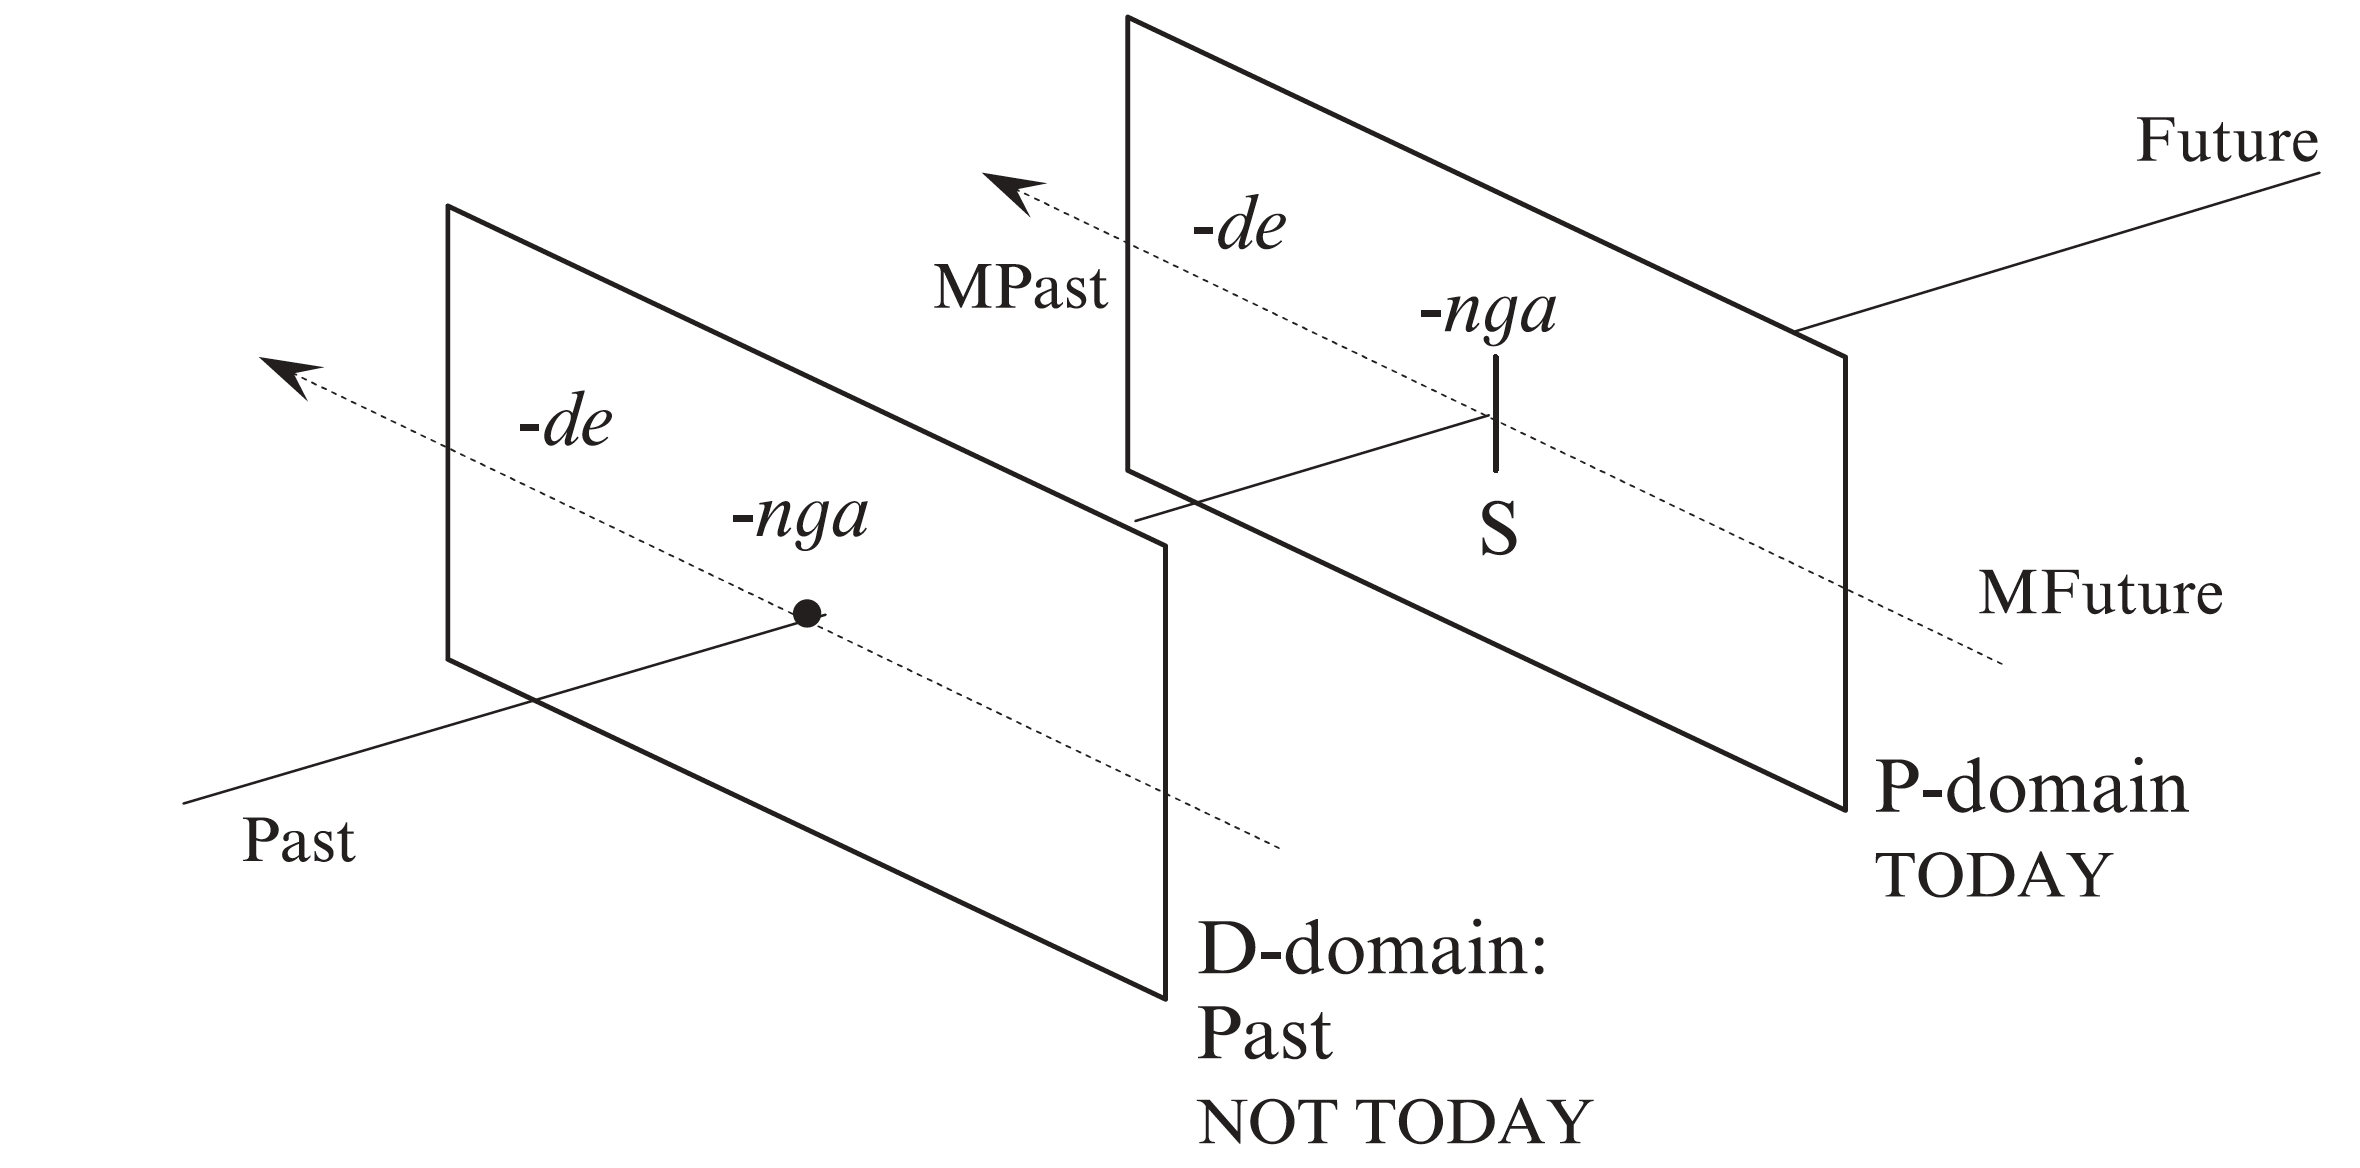
\includegraphics[width=0.9\linewidth]{botnecogdoms}
\end{figure}

\subsection{\textit{Énonciation}, diachrony \& functional unity}

For all the talk of reference frames and cognitive domains, how much closer are we to understanding the motivations for a the encoding of complex temporal remoteness systems of a grammaticalised cyclic tense system?

A number of linguists working on temporal/aspectual distinctions made in Indo\-European languages have drawn \citeauthor{Benveniste1966}'s distinction between ``narrative'' (\textit{récit\slash{}histoire}) and \textit{discours} modes (\textit{plans d'énonciation}).\footnote{Where ``\textit{\textbf{l'énonciation historique} [...] s'agit de la présentation des faits survenus à un certain moment de temps, sans aucune intervention du locuteur dans le récit}'' and \textit{\textbf{discours}} constitutes ``\textit{toute énonciation supposant un locuteur et un auditeur, et chez le premier l'intention d'influencer l'autre en quelque manière}''
	
	(``\textbf{Narrative} comprises the presentation of facts already having occurred at a given moment in time, without any intervention on the part of the speaker'' whereas \textbf{discourse} is understood as ``any utterance that presupposes a speaker and a hearer, where the former intends on influencing their interlocutor in some way.'')\trailingcitation{
	 \citetext{\citealp[238--42]{Benveniste1966}; translation and emphasis mine.}}} To take one example, \citeauthor{Duchet2016}'s \citeyearpar{Duchet2016} study of the usage domains of the Albanian [\gls{sqi}] \textit{\textsc{aorist}} and \textit{\textsc{perfect}},
 \footnote{That is, the synthetic `\textsc{aorist}' (\textit{e kryer e thjeshtë}) and the periphrastic `\textsc{perfect}' \textit{(e kryer)} form `\textsc{have}+past participle' respectively.} suggests the possible utility of this broad \textit{``énonciative''} dichotomy in understanding the distibution of these forms. While past-referring event descriptions in narrative contexts are the \textit{locus classicus} of the \textit{Aorist}, \citeauthor{Duchet2016} show that, in discourse contexts, using this form is also possible in a number of other apparent uses --- including the description of present-holding result states and ``immediate future'' accomplishments. The  \textit{Perfect}, traditionally encoding ``presently relevant result states'' (co-occurring frequently with TFAs that include speech time (`today/this week/this year') and in narratives to encode ``hot news'', also has a range of anterior-type uses: describing states (possibly) occurring prior to (\textsc{aorist-})marked past events.
 
Relatedly, in a survey of remoteness distinctions, \citet[116\textit{ff}]{Dahl1983} identifies a number of languages that appear to treat past differently in ``narrative contexts,'' going on to propose a number of cross-linguistic generalisations that seek to motivate a ``tendency to neutralize distance distinctions in narrative contexts.'' Drawing on a proposed distinction between narrative and discursive contexts, it is conceivable the two reference frames (\textsc{today\slash{}pre-today}) featuring into our analysis of \textsc{wd} temporal reference, in some sense, correspond respectively to \textbf{conversational} and \textbf{narrative} modes. 
 
 That is, in \textbf{conversational} contexts, described events are likely to bear a more immediate relation to the present. Here, a discourse is likely to be concerned with a distinction between {\color{blue}\textsc{past}} and {\color{forest}\textsc{nonpast}}. Conversely, in \textbf{narrative} contexts (accounts of exclusively past events), the distinction between events that held in a {\color{blue}\textsc{remote}}, inaccessible past versus those that held in a relatively \textsc{\color{forest}{recent}} one that more closely resembles the here-and now.\footnote{Compare \citeauthor{Waters1989}'s observation (in his description of Djinaŋ's \textsc{today/remote past}) that ``few stories are set in the time context of the same day as the speech event'' \citeyearpar[188]{Waters1989}.} This usage evokes the phenomenon of the ``narrative/historic present'' --- a commonly attested use cross-linguistically  \citetext{see \citealp{Carruthers2012} for an overview}.\footnote{Cited by \citet[312]{Carruthers2012}, \citeauthor{Facques2007} claims that the historic present ``permet de maintenir l’illusion d’une perspective simultanée du récit, déjà induite par l’emploi du present” (``
 	allows the	illusion to be maintained that the events and the narrative are simultaneous, an illusion already created by use of the present”) \citetext{\citeyear[250--1]{Facques2007}, Carruthers' translation.}} A similar usage of the \textsc{pres} (or \textsc{nonfuture}) is also pointed out by \citet{Stirling2012a}, who shows its extensive use in Kalaw Lagaw Ya [\gls{mwp}], where it functions as a past perfective in narrative contexts.\footnote{This type of usage is apparently widespread in Arnhem Land languages \citetext{\citealt[\textit{e.g.},][]{Bednall2019} for Anindilyakwa [\gls{aoi}]}}
 
On this account, the emergence of \textit{cyclic tense} of the type exhibited in the languages of Maningrida and the westernmost Yolŋu varieties (\textit{viz.} Djinaŋ, Djinba and \gls{wd}) can be explained in terms of a categoricalisation of these two ``reference frames'' that are closely associated with different modes of language use. This corresponds to a hypothetical analysis where: 
\begin{itemize}
	\item Language is used for conversation (pertaining to the eventualities that relate to the here-and-now) and for storytelling (pertaining to events completed prior to the here-and-now)
	\item The function of a \textsc{past}-tense is to signal the settledness and completeness of an event vis-à-vis utterance time. The function of \textsc{present} tenses indicates that the runtime of an event overlaps with utterance time.
	\item The \textsc{past}/\textsc{present} distinction gets reanalysed as \textsc{precontemporary}-{\sc contemporary}: that is \textsc{past/present} relative to a given reference frame (as determined by context (functions) of the utterance.)
\end{itemize}

\subsection{Aspect \& temporal interpreation}
As shown in \S~\ref{sec:djr-prs}, \textsc{wd} verb stems have a strictly dynamic (state change) semantics, a fact that seems to correspond with the recruitment of new strategies for encoding aspectual and modal information (primarily through preverbal auxiliaries and particles.)\footnote{Whereas an explicit aspectual (±\textsc{ipfv}) distinction is actually grammaticalised in the Djinaŋ verbal paradigm, a feature not shared by other Yolŋu languages} The development of this analytic TMA marking system in Dhuwal-Dhuwala is likely to be related to the emergence of a ``cyclic tense'' system where \gls{I} (the erstwhile `\gls{pres}') now obligatorily co-occurs with \textit{ga} `\gls{ipfv}' in order to encode present reference. Compare this fact to the incompatibility between present reference and achievement predicates, where a sentence of the type exemplified in (\nextx) is only available with either a historic present or immediate future reading \citep[an observation following][147]{Vendler1957}.


\pex\textit{Now they find the treasure/win the race/reach the summit}\xe
\pex\a\begingl\gla ŋarra *(ga) \textbf{ḻuka} mänha (dhiyaŋu~bala)\deftagex{wd-contemp}\deftaglabel{prog}//
\glb 1s \gls{ipfv}.\gls{I} drink.\gls{I} water now//
\glft`I'm drinking water (now).'\trailingcitation{[DB~20190405]}//\endgl
\a\begingl\gla ŋarra *(dhu) \textbf{ḻuka} mänha (dhiyaŋu~bala)\deftaglabel{fut}//
\glb 1s \gls{fut} drink.\gls{I} water now//
\glft`I'm going to drink water (now).'\trailingcitation{[DB~20190405]}//\endgl
\a\begingl\gla ŋarra \textbf{ḻuka} mänha (barpuru)//
\glb 1s \gls{ipfv}.\gls{I} drink.\gls{I} water//
\glft`I drank water yesterday.'\trailingcitation{[DB~20190405]}\deftaglabel{pst}//\endgl

\xe

This resembles the situation in \textsc{wd} (\getref{wd-contemp}), where \gls{I} necessarily co-occurs with \textit{ga} `\gls{ipfv}.\gls{I}' or \textit{dhu} `\gls{fut}' to encode present (progressive) or immediate future reference. In the absence of either of these markers, only the \textsc{recent (non-today) past} reading is felicitous.

The relationship between the emergence of cyclic tense in \gls{wd} and evidence for a wholesale restructuring of the language's aspectual system remain a subject for considerable further work and analysis.

\fancybreak

\noindent In view of the semantics for \gls{I} and \gls{III} above, this section has considered possible candidates for functional motivations for the notion of the ``reference frame'' and the ``recycling'' or ``temporal discontinuity'' of tense markers that characterise cyclic tense. On the basis of these considerations, (\nextx) formulates a hypothesis for the emergence of a cyclic tense system of the type described here.

\pex \textbf{\textsc{diachronic hypothesis.}\\Cyclicity as the grammaticalisation of text type}\\
The cyclic tense phenomena exhibited in \textsc{wd} and related languages are a result of the reanalysis of \textsc{present}- and \textsc{past}-tense markers' apparently divergent usage in conversational versus narrative contexts
\xe




 

\section{Conclusion}


This chapter has provided analyses for a number of phenomena related to the temporal interpretation of \textsc{wd} predicates. Of particular importance for developing an analysis of the \textsc{wd} paradigm and \gls{wd}'s tense system is the notion of \textsc{precontemporary instantiation}, a motivation for which was the primary focus of \S~\ref{sec:cyc}.

Drawing on descriptions from \citet{Glasgow1964} and subsequent treatments of the languages of western and central Arnhem Land \citep{Green1987,Green1995,Wilkinson1991,Eather2011,Waters1989}, we proposed a formal treatment of the notion of the ``reference frame'' --- effectively a \textsc{hodiernal/prehodiernal} dichotomy in the \textsc{nonfuture} (``\textsc{realis/actual}'') domain which corresponds to a superinterval of the reference time.

It was argued that the contribution of \gls{III} (the \textsc{precontemporary}) is to constrain reference time to a \textsc{non-final} subinterval of the contextually-supplied reference frame. Via blocking, instantiation of predicates inflected with \gls{I} are felicitous only within the complement of \gls{III}'s range within the realis domain. That is, \gls{I} --- an inflection compatible with present, past and future reference --- is an unmarked form, temporally neutral in its semantics \citetext{compare to treatments of the present, \textit{e.g.}, \citealp{Fleischman1990,Carruthers2012}.\footnote{Also \citeauthor{Dahl1983}'s generalisation that ``[i]t is almost always possible to use the least marked indicative verb form in a narrative past context'' (\citeyear[117]{Dahl1983}, \textit{apud} \citealt{Dahl1980} \textit{n.v}.)}}

 The following chapter extends the account to \gls{II} and \gls{IV} --- the irrealis categories.

%\begin{quote}\small Such meanings probably develop through the interaction of the meaning of the two grams. If a hodiernal past and an anterior (with current relevance) are both developing in the language they would both have a claim to describe situations having just occurred on the same day. If the anterior wins for situations that just occurred but the hodiernal continues to function for situations earlier in the same day, then the result is a discontinuous meaning for the non-hodiernal gram.\trailingcitation{\citep[104]{Bybee1994}}\end{quote}


%\pex
%
%\a \begingl\gla  ŋarra rur'yuna yurruna walu dha-barkthurruna//
%\glft`.'//\endgl
%
%

%
%\xe


\chapter{Modal interpretation \& \textsc{negative asymmetry}\\{\large\sc distinguishing $\boldmath{ \langle \gls{I},\gls{III}\rangle}$ from $\boldmath{ \langle \gls{II},\gls{IV}\rangle}$}}\label{sec:yol-mood}

The basic distributional facts for \gls{II} and \gls{IV} were described in \S~\ref{djr-infl}. As shown there, verb stems receive \gls{II}-marking in future-oriented predications (including imperatives), whereas \gls{IV}-marking is associated most clearly with counterfactual predications and other modal claims with past temporal reference. On the basis of these data, these two inflectional categories appear to be associated with \textit{non-realised} events; and it is this property that distinguishes them from the \gls{I}- and \gls{III}-marked verbs described in the previous chapter (ch.~\ref{sec:djr-temp}).

In this chapter, we interrogate the nature of this apparent ``reality status'' distinction drawn in \gls{wd} (as it is in other Yolŋu Matha varieties) and the expression of mood, modality and modal operators in \gls{wd} more broadly. The distinction between $\langle \gls{I},\gls{III}\rangle$ and $\langle \gls{II},\gls{IV}\rangle$ is ultimately to be understood as one of \textsc{verbal mood}. One phenomenon of particular interest is that of an apparent kinship between negative operators (sentential negators) and modal operators as they are realised in \gls{wd}. It is this kinship that looks to undergird \textit{asymmetric negation} in \textsc{wd} with respect to the marking of reality status; a description of this phenomenon is the goal of \S~\ref{sec:negs}.

\section{Sentential negation and paradigm neutralisation}\label{sec:negs}

As shown in our discussion of the Negative Existential Cycle in Yolŋu Matha (\S~\ref{NEC-yolŋu}, see \textit{p.}~\pageref{sec:nec-djr}), Djambarrpuyŋu has two particles---\textit{yaka} and \textit{bäyŋu}---which both realise standard negation (\textit{i.e.}, that operator whose effect is to reverse the truth value of a given proposition.) The primary distributional distinction between these is that only \textit{yaka} is used to generate negative imperatives (prohibitives) whereas only \textit{bäyŋu} is found in negative existential/quantificational contexts (\getref{bayŋu-negq}--\getref{yaka}). Of interest for current purposes however, is the fact that both of these sentential negators can be shown to directly interact with verbal inflection.


Descriptively, as shown in the data in (\getref{neg-pres}--\getref{neg-pst}), negation appears to trigger a ``switch'' from the `realis-aligned inflections' (\gls{I}~and~\gls{III}) to their `irrealis counterparts' (respectively \gls{II}~and~\gls{IV}). As shown, these latter categories otherwise turn up predominantly in \textit{hypothetical} or \textit{counterfactual} contexts. As we will see, this points to an analysis where the Western Dhuwal(a) inflectional system encodes a \textit{reality status}-based distinction that is neutralised in negated sentences \citep[see also discussion in][356]{Wilkinson1991}. This effect --- which we term a ``negative asymmetry'' \citep[specifically \textsc{\texttt{a/nonreal}}, following][]{Miestamo2005} --- was introduced above (\S~\ref{sec:asymneg}, compare the Gurr-goni \gls{gge} data in \getref{sn-gvg})  and is summarised below in Table \ref{tab:negneut}. Here, we develop a theory of the negative asymmetry as an epiphenomenon of a kinship between \textsc{negative} and (other) \textsc{irrealis} operators.

\begin{table}[h]\centering
	\begin{tabular}{ccc}
		&\multicolumn{2}{c}{\textsc{\textbf{polarity}}} \\
		& \textsc{--neg} & \textsc{+neg}\\\midrule
		&	\gls{I} & \multirow{2}{*}{\gls{II}}\\
		& \gls{II} \\\midrule
		&	\gls{III} & \multirow{2}{*}{\gls{IV}}\\
		& \gls{IV} \\\bottomrule
	\end{tabular}
	\caption{Neutralisation of \gls{I} and \gls{III} inflections under negation.}\label{tab:negneut}
\end{table}


The following examples in (\getref{neg-pres}) show how sentences that receive \gls{I}-marking in positive sentences --- encoding temporal reference to the present or recent past (Ch.~\ref{sec:djr-temp}) --- instead receive \gls{II}-marking under the scope of negation. Each example contains a predication about the present or about the recent past (normally the domain of \gls{I}, as described in the previous chapter.) In thje presence of a negative operator, however, the verb receives \gls{II}-marking. 

(\getref{neg-pres}a-b), for example, presents a near-minimal pair, where the inflection received by a predicate with present reference ``switches'' from \gls{I} to \gls{II} under negation.

\pex\textbf{Exponence of present and recent past reference as \gls{II} under negation}
\deftagex{neg-pres}


\a\begingl%\glpreamble Present-tensed sentence with \gls{I}//
\gla Nhaltja-\textbf{n} \textbf{ga} limurru-ŋgu-ny rom waŋ-\textbf{a}?//
\glb do.how-\gls{I} \gls{ipfv}.\gls{I} 1p.\gls{incl}-\gls{dat}-\gls{prom} law say-\gls{I}//
\glft`What does our law say?'\trailingcitation{\citepalias[~Luk~14.3]{DB}}//\endgl

\a\begingl%\glpreamble Negated present-tense sentence receives \gls{II} marking//
\gla \textbf{yaka} \textbf{gi} \textbf{biyak} rom waŋ-\textbf{i}//
\glb \textbf{\gls{neg}} \gls{ipfv}.\gls{II} do.thusly.\gls{II} law say-\gls{II}//
\glft`That's not how the law is/what the law says.'\trailingcitation{\citep[357]{Wilkinson1991}}//\endgl 




\a\begingl%\glpreamble  Negated present-tense sentence receives \gls{II} marking\\\textsc{context.} Speaker is trying to read from a computer screen.//
\gla \textbf{bäyŋu} ŋarra \textbf{gi} nhä-\textbf{ŋu}//
\glb \textbf{\gls{negq}} 1s \gls{ipfv}.\gls{II} see-\gls{II}//
\glft`I can't see (it).'\\
%\textsc{comment.} \textit{nhäŋu} (`see.\gls{II}') could also mean yesterday in past.
\textsc{\textbf{comment.}} `I didn't see (it) (yesterday)' is also an available reading.\trailingcitation{[AW 2018030]}//\endgl



\a\begingl\gla Ŋarra \textbf{gi} bäyŋu maḻŋ'mara-\textbf{ŋu} waṯu (ŋarraku). + Bili ŋayi \textbf{ga} nhin-\textbf{a} wäŋaŋura//
\glb 1s \textsc{ipfv}.II \gls{neg} appear.\gls{caus}-\gls{II} dog 1s.\gls{dat} \gls{cplv} 3s \gls{ipfv}.\gls{I} sit.\gls{I} house.\gls{loc}//
\glft`I can't find my dog. It lives in the house.'\trailingcitation{[DhG~20190417]}//\endgl



\a\begingl\gla Ŋarra ga djäl-thi-\textbf{rri} giritjirrinyara-wu, + yurru ŋarra bäyŋu-nha \textbf{girritji}//
\glb 1s \gls{ipfv}.\gls{I} want-\gls{vblzr}-\gls{I} dance.\gls{nmlzr}-\gls{dat} but 1s \gls{neg}-\gls{seq} dance-\gls{II}//
\glft`I was wanting to dance (at the \textit{buŋguḻ} yesterday) but I didn't dance (because I'd hurt my leg yesterday.)'\trailingcitation{[DhG~20190417]}//\endgl
%\a\begingl\glpreamble\textsc{context.} A recent hunting trip, narrated in \gls{I} for corresponding positive descriptions.//
%\gla ga \textbf{yaka} ŋayi ŋunhi dharyu-\textbf{rr} \textbf{biyak} djin'tjiŋdhu-\textbf{rr}//
%\glb and \textbf{\gls{neg}} 3s \gls{texd} rain-\gls{II} do.thusly.\gls{II} rain~lightly.\gls{II}//
%\glft`...and it did not rain lightly'\trailingcitation{\citep[357]{Wilkinson1991}}/endgl
\xe


Similarly, in contexts where the temporal reference of the event description predicts that the verb will receive \gls{III}-inflection --- following our description from Ch. \ref{sec:djr-temp}, when referring to the same-day (\textsc{hodiernal}) or the remote past --- when co-occurring with a negative particle (\textit{yaka/bäyŋu}), the verb instead receives \gls{IV}-inflection. This is shown by the data in (\getref{neg-pst}).

 Again, (\getref{neg-pst}a-b) represents a minimal pair where negative marking triggers a ``switch'' from \gls{III} to \gls{IV} inflection. (c) shows the negation of an immediate past event licensing \gls{IV} inflection, (d) shows how a negated, \gls{IV}-inflected predicate can be embedded under a propositional attitude predicate to encode a false belief, and (e) an example of a negated description of the remote past receives \gls{IV} inflection.

\pex \textbf{Exponence of \textsc{today past} and \textsc{remote past} reference as \gls{IV} under negation}\deftagex{neg-pst}
%\a\deftaglabel{munha}\begingl\gla bäyŋu ŋarra gäthur ŋorra-\textbf{nha} manymak-ku-\textbf{nha} munhawu//
%\glb \gls{negq} 1s today lie-\gls{IV} good-\gls{tr}-\gls{IV} nighttime//
%\glft`I didn't sleep well last night'\trailingcitation{\citep[357]{Wilkinson1991}}//\endgl

%\mcom{Though the second clause in (b) also has ŋuli so maybe this is not quite so nice an ex. as originally thought}\a\begingl\gla ŋäthil-nydja ŋarra ga-n dhuwal, ga miltjiri marrtji-n \ bäyŋu ŋarra ŋuli ga-\textbf{nha} nhä-\textbf{nha}//
%\glb earlier-\gls{prom} 1s \gls{ipfv}-\gls{III} \gls{prox} and blind go-\gls{III} \textbackslash \gls{negq} 1s \gls{hab} \gls{ipfv} see-\gls{IV}//
%\glft`I was blind before; I was unable to see'\trailingcitation{\citep[358]{Wilkinson1991}}//\endgl


\a\begingl\gla gathur munhagumirr ŋarra nhä-\textbf{ŋal} warrakan//
\glb today morning 1s see-\gls{III} bird//
\glft`I saw a bird this morning'\trailingcitation{[FW 20180802]}//\endgl


\a\begingl\gla gathur munhagumirr \textbf{bäyŋu} ŋarra nhä-\textbf{nha} warrakan//
\glb today morning \textbf{\gls{negq}} 1s see-\gls{IV} bird//
\glft`I didn't see a bird this morning'\trailingcitation{[FW 20180802]}//\endgl

\a\begingl\glpreamble \textsc{\textbf{context}.} Speaker has dropped a coin.//
\gla Way! \textbf{Bäyŋu} ŋarra nhä-\textbf{nha}?//
\glb Hey! \textbf{\gls{negq}} 1s see-\gls{IV}//
\glft`Ah! Did you see (it)?'\trailingcitation{[AW 20180830]}//\endgl


\a\begingl\glpreamble\textbf{\textsc{context.}} I'm at work explaining to my coworker why my \textit{galay} is angry at me.//
\gla Ŋarraku miyalk maḏakarritj-thi-\textbf{na} bili ŋayi ga \textbf{guyaŋa} ŋarra ga-\textbf{nha} bäyŋu djäma//
\glb 1s.\gls{dat} wife anger-\gls{inch}-\gls{III} \gls{cplv} 3s \gls{ipfv}.\gls{I} think.\gls{I}\footnotemark{} 1s \gls{ipfv}-\gls{IV} \gls{neg} work//
\glft`My wife got angry because she thought I wasn't working today.'\trailingcitation{[DhG~20190417]}//\endgl

\a\begingl\glpreamble \textbf{\textsc{context.}} The speaker grew up in the desert.//
\gla \textbf{bäyŋu} ŋarra ŋuli ga-\textbf{nha} nhä-\textbf{nha} (waltjaṉ) ŋunhi ŋarra yothu yän//
\glb \textbf{\gls{neg}} 1s 	\gls{hab} \gls{ipfv}.\gls{IV} see.\gls{IV} rain \gls{texd} 1s child just//
\glft`When I was young, I hadn't seen [rain]/never saw [rain].'\trailingcitation{[AW~20190501]}//\endgl\xe


%\mcom{It's not clear how I can easily get a the status of this alternation via elicitation (esp. if its intraspeaker..?) or whether I should just abstract away from it. My informants so far seem to have consistently respected this alternation.}
%todo comments about variation across Dhuwal/a
%	Generally, there seems to be a perception (Melanie Wilkinson \textit{pers. comm.}, independently supported by consultant AW [20180830]) that the maintenance of \gls{I} and \gls{III} (the `\textsc{realis}-aligned' inflections) under negation is a characteristic of \textit{Miwatj} varieties of Dhuwal-Dhuwala (\textit{i.e.}, those spoken in towards the East.)
%	
%	\mcom{There's a great comment from my consultant in her translation of a negative sentence. When asked why \textbf{\textit{gi+}II} was used instead of \textbf{\textit{ga+}I} she claims `not happening yet' (20180802-8min)}\citet[356]{Wilkinson1991} notes that ``[she has] not been able to determine a functional basis for this alternation.'' Nevertheless, in his typological survey of standard negation, \citet[558]{Miestamo2005} identifies a cross-linguistically attested mood-based asymmetry where negative marking triggers the appearance of the irrealis or other ``nonrealised''-type modal markings. This phenomenon seems to be particularly well-represented in the languages of the Top End, functional explanations generally emphasising the fact that negated predicates `[belong] to the realm of the non-realized', a domain associated with irrealis marking (\citealt[225]{Miestamo2005}, cf. \citealt[195]{McLellan1992}, \citealp[see also][]{Phillips2019}). These ideas are explored in further detail in Chapter \ref{anY} below.
%	
%	\citet{Wilkinson1991} also suggests that there is insufficient cross-linguistic data to assess a the diachrony (and potential areal diffusion) of this asymmetry (356), although provides a concise review of other authors' observations of Yolŋu varieties (359-60). Data about the interactions between polarity and verbal inflection are provided in the following sections and the question of the development of these asymmetries is treated in Chapter \ref{diaY} below.

The data in (\getref{neg-pres}--\getref{neg-pst}) evince a species of \textsc{negative asymmetry} that is manifested in \gls{wd}. That is, from the four inflections which are availble for encoding temporal and modal information in \gls{wd}, only two (\textit{viz.} \gls{II} and \gls{IV}) are felicitous in sentences that are negated by \textit{yaka} or \textit{bäyŋu}. Figure \ref{NegSchem} schematises the relationship between temporal reference and inflection selection in \textbf{negative clauses} (\textit{cf.} Fig.~\ref{TempSchem}, \textit{p.}~\pageref{TempSchem}.)


\begin{figure}[h]\centering\caption{Apparent interactions between temporal relations and reality status in Djambarrpuyŋu: cyclicty and metricality under negation.}\label{NegSchem}
	\begin{tikzpicture}[scale=1.2]
		% draw horizontal line   
		\draw[<->, line width=.5mm] (0,0) -- (12,0);
		
		%draw rex
		\shade[left color=violet!15!white, right color=orange!15!white] (0,0.02) rectangle (4.8,1.5);
		%	\fill[green!10!white] (2.5,0.02) rectangle (4.8,1.5);
		\fill[violet!10!white] (4.8,0.02) rectangle (6.8,1.5);
		\shade[left color=orange!10!white, right color=green!10!white] (6.8,0.02) rectangle (9.5,1.5);
		\fill[orange!10!white] (9.5,0.02) rectangle (12,1.5);
		
		% draw nodes
		\draw (1.25,0) node[below=3pt] {\textbf{}} node[above=15pt] {\textsc{\gls{IV}}};
		\draw (3.675,0) node[below=3pt] {\textbf{}} node[above=15pt] {\gls{II}};
		\draw (5,0)   node[circle,fill,label=below:$\lfloor{\sl today}$] {} node[below=3pt] {\textbf{}} node[above=3pt] {};
		\draw (7,0) node[diamond,shade,inner color=ochre,outer color=black,label=below:$\boldsymbol{t*}$] {} node[below=3pt] {\textbf{}} node[above=3pt] {\textsc{}};
		\draw (5.8,0) node[below=3pt] {\textbf{}} node[above=15pt] {\textsc{\gls{IV}}};	
		\draw (7.5,0) node[below=3pt] {\textbf{}} node[above=15pt] {\textsc{\gls{II}}};
		\draw (9,0) node[below=3pt] {\textbf{}} node[above=15pt] {\textsc{\gls{I}}};	
		\draw (10.75,0) node[below=3pt] {\textbf{}} node[above=15pt] {\textsc{\gls{II}}};	
		\draw (9.5,0)   node[circle,fill,label=below:${\sl today}\big)$] {} node[below=3pt] {\textbf{}} node[above=3pt] {};
		
		%		%braces
		%		\phantom{	\draw [decorate,decoration={brace,amplitude=4pt},xshift=-0pt,yshift=35pt]
		%			(0.5,0.5) -- (4.5,0.5) node [black,midway,yshift=0.35cm] 
		%			{\footnotesize metricality};
		%
		%			\draw [decorate,decoration={brace,amplitude=4pt},xshift=-0pt,yshift=40pt]
		%			(3.5,0.5) -- (9,0.5) node [black,midway,yshift=0.35cm] 
		%			{\footnotesize cyclicity};}
		
	\end{tikzpicture}
\end{figure}

Further complicating things, while \gls{III} is categorically ruled out in negative sentences, \gls{I} ``survives'' when (and \underline{only when}) the predicate refers to the \textsc{same-day future.} That is, the \gls{I}/\gls{II} distinction is \textit{not} neutralised in negative sentences with reference to events happening later on the day of utterance (whereas the distinction \textit{is} neutralised in all \textsc{nonfuture} contexts.) Examples are provided in (\getref{futneg}-\getref{prsneg}).


\pex \textbf{Future marking is unaffected by polarity/the presence or absence of sentential negation}	\deftagex{futneg}
\a\begingl\glpreamble \gls{I} with \textsc{same-day future} reference ``survives'' negation//
\gla ŋarra (yaka) ŋunha \textbf{dhu} ḻuk-\textbf{a} dhiyaŋ~bala//
\glb 1s (\gls{neg}) \gls{fut} \gls{dist} eat-\gls{I} now//
\glft`I will (not) eat them [\textit{ḻatjin}] right now.'\trailingcitation{[AW~20190422]}//\endgl

\a\begingl\glpreamble \textsc{post-hodiernal} referring predicates receive \gls{II}-inflection//
\gla (bäyŋu) ŋarra \textbf{dhu} buḻ'yu-\textbf{rr} barpuru//
\glb \gls{neg} 1s \gls{fut} play-\gls{II} tomorrow//
\glft`I will (not) play [football] tomorrow.'\trailingcitation{[AW~20190429]}//\endgl
\xe

\pex \textbf{A minimal pair: \gls{I} changes to \gls{II} in present-referring negative sentences}\deftagex{prsneg}
\a\begingl\glpreamble Negative present predication with \gls{II}//
\gla (dhiyaŋ~bala) \textbf{bäyŋu} ŋarra \textbf{gi} nhä-\textbf{ŋu} mukulnha//
\glb now \textbf{\gls{neg}} 1s \gls{ipfv}.\gls{II} see-\gls{II} aunt.\gls{acc}//
\glft`I don't/can't see my aunt (right now).'\trailingcitation{[AW~20190501]}//\endgl
\a\begingl\glpreamble Positive present predication with \gls{I}//
\gla (dhiyaŋ~bala)  ŋarra \textbf{ga} nhä-\textbf{ma} mukulnha//
\glb now 1s \gls{ipfv}.\gls{I} see-\gls{I} aunt.\gls{acc}//
\glft`I'm watching my aunt (right now).'//
\endgl\xe


\section{The meaning of the modal particles}
\label{sec:modals}
%todo label `anY' has been de-defined
%\section{The realm of the nonrealized}\label{anY}
In \S~\ref{djr-infl}, we saw that predicates which receive \gls{II}- and \gls{IV}-inflection co-occur with some operator that encodes some flavour of irrealis-associated meaning --- suggesting what \citet[145]{Palmer2001} labels a ``joint marking system'' (\textit{i.e.}, that reality is multiply indicated, in this case by suffixation in addition to a preverbal particle.) 

For \gls{II}, these are predominantly represented by \textit{dhu} `\gls{fut}' and \textit{balaŋ(u)} `\gls{irr}' in addition to clauses with imperative syntax. \gls{IV} tends to co-occur with \textit{balaŋ} `\gls{irr}' in addition to \textit{ŋuli} `\gls{hab}'.\footnote{I adopt the (metalinguistic) labels \gls{fut} for \textit{dhu} \citep[following][]{Wilkinson1991} and \gls{mod} for \textit{balaŋ(u)}. As we will see, these descriptions aren't necessarily completely semantically adequate, but will be sufficient for current purposes. \citet{Wilkinson1991} glosses \textit{ŋuli} as `\gls{hab}' or `\gls{hyp}' depending on its apparent function in the clause (as a marker of \textsc{habituality} or of a conditional antecedent (``\textsc{hypotheticality}'').)\label{irr-glossing}} Importantly, and as we will see, these expressions all appear to lexicalise strictly \textbf{root} (circumstantial\slash{}non-epistemic) modalities \citep[\textit{contra claims in}][123]{VanderWal1992}.

This section seeks to model the irrealis domain using the ``branching time framework'' introduced in \S~\ref{LitRev} in order to propose a semantics for \gls{wd} modal particles. This will permit for forming a set of generalisations over the distribution of \gls{II} and \gls{IV}.



	%\subsection{The branching time framework}\label{sec:wd-BT-fwk}
	%
	%Authors working in intensional semantics have, in recent work, deployed a ``branching time'' framework in order to model relationships between temporal and modal reference (an overview provided in Chapter \ref{IntroCh} and implemented in the semantic treatment of \textit{bambai} in Chapter \ref{bambai.semx}). Here, I spell out a number of basic assumptions that will ultimately assist in formalising temporal and modal expressions in WD. One of the primary payoffs of the branching time is the formalisation of Prior's observations about the asymmetries of the past and the future \citep[see also][]{Copeland2020,Dowty1977,Thomason1970,Thomason1984}. The version I adopt here follows closely from recent work on the realis-irrealis distinction \citep{VonPrince2019,Krifka2016} and other insights about temporal and modal interaction (\citealp[e.g.][]{Condoravdi2002,Ippolito2013}, a.o.)
	%
	%
	%A branching-time frame $ \mathfrak U=\langle \mathcal I,\prec\rangle $ assumes a partially ordered set of indices $ \mathcal I $ --- in effect world-time pairs $ \langle w,t\rangle  $. A branch (similar to ``history'' for other authors \citep{Thomason1970,Dowty1977}) $ b\ni i $ through any $ i\in\mathcal I $ is a linearly ordered subset of $ \mathcal I $ --- that is, where $ i=\langle w,t\rangle $,\\ $ b\ni i=\{\big\langle\langle w,t\rangle,\langle w,t'\rangle,\langle w,t''\rangle,\hdots,\langle w,t_n\rangle\big\rangle\}$. A branch, then, effectively models the possible development of a given world through time.\footnote{Note that these frameworks normally take indices to represent world-time pairs. I assume that this model can be extended relatively straightforwardly to capture interval semantic notions (\citealp[e.g.][]{Landman1991,Dowty1982,Bennett} a.o.).}
	%\begin{figure}[h]
	%	\caption{A branching times frame following von Prince \citeyearpar[e.g.,][591]{VonPrince2019}. Vertically aligned indices are taken to index the same time.}\centering
	%	\begin{tikzpicture}
	%		[scale=1.5,level distance=9mm,
	%		every node/.style={fill=black,circle,inner sep=1.5pt},
	%		level 1/.style={sibling distance=10mm},
	%		level 2/.style={sibling distance=8mm},
	%		level 3/.style={sibling distance=4mm},
	%		level 4/.style={sibling distance=2mm},
	%		edge from parent/.style={draw}]
	%		\node {} [grow=right]
	%		child {node {} edge from parent[densely dotted]
	%			child {node {}
	%				child {node {}
	%					child {node {}}
	%					child {node {}}}
	%				child {node {}
	%					child {node {}}
	%					child {node {}}}}
	%			child {node {}
	%				child {node {}
	%					child {node {}}
	%					child {node {}}}
	%				child {node {}
	%					child {node {}}
	%					child {node {}}}}}
	%		child[missing]
	%		child {node {}
	%			child {node {} edge from parent[densely dotted]
	%				child {node {}
	%					child {node {}}
	%					child {node {}}}
	%				child {node {}
	%					child {node {}}
	%					child {node {}}}}
	%			child {node {} edge from parent[densely dotted]
	%				child {node {}
	%					child {node {}}
	%					child {node {}}}
	%				child {node {}
	%					child {node {}}
	%					child {node {}}}}
	%			child {node [style={fill=red},label=above:$ \boldsymbol{i*} $] {}
	%				child {node {} edge from parent[densely dashed]
	%					child {node {}}
	%					child {node {}}}
	%				child {node {} edge from parent[densely dashed]
	%					child {node {}}
	%					child {node {}}}}};
	%\end{tikzpicture}\end{figure}
	%
	%
	%
	%
	%
	%
	%
	%\Citet{VonPrince2017a,VonPrince2019} establishes a formal trichotomy between the \textsc{actual, potential} and \textsc{counterfactual} domains by appealing to this framework. This is reproduced in (\nextx).
	%
	%\pex Given a contextually defined \textsc{actual present} $( i*=\langle w*,t*\rangle )$, $ \mathcal I $ can be partitioned into three subdomains:
	%\a The \textsc{actual} (past/present) = $ \{i\mid i\preceq i*\} $\\
	%Compare this notion to the equivalent one of \textit{metaphysical alternatives to $ w $ at $ t $} introduced in Ch. \ref{bambai}: $ \{w'\mid w\approx_t w\} $.
	%\a The \textsc{potential} (future) = $ \{i\mid i\succ i*\} $
	%\a The \textsc{counterfactual} = $ \{i\mid i \text{ is unordered w/r/t } i* \} $\deftagex{trichot}\deftagpage{vP-bt}
	%\xe





\subsection{\textit{dhu}: irreality and the \textsc{future}}

Shown above (predominantly in \S~\ref{desc-ii}),  \textit{dhu} `\gls{fut}' occurs in sentences with future temporal reference -- with either \gls{I} or \gls{II} marking, depending on whether the reference time of the proposition is the same as the day of speech or beyond. This is shown again by the data in \getref{dhu-fut}.

Relatedly, the data in (\getref{dhu-nec}) show that \textit{dhu} appears to also be compatible with other circumstantial modalities; for example, with (\getref{dhu-nec.d}) deontic, (\getref{dhu-nec.b}) bouletic and (\getref{dhu-nec.t}) teleological readings. In all these contexts, we can model \textit{dhu} as universally quantifying over a (subset of) a circumstantial modal base.

\pex \textbf{\textit{dhu} `\gls{fut}' encoding future tense with \gls{I}- and \gls{II}-inflections}
\a\begingl\gla barpuru goḏarr ŋarra \textbf{dhu} nhä-\textbf{ŋu}//
\glb funeral tomorrow 1s \gls{fut} see-\gls{II}//
\glft`I'll watch the funeral tomorrow.'\trailingcitation{}\deftagex{dhu-fut}//
\endgl
\a\begingl\gla mukul \textbf{dhu} \textbf{gi} nhin-\textbf{i} raŋi-ŋur goḏarr//
\glb aunt \textbf{\gls{fut}} \gls{ipfv}.\gls{II} sit-\gls{II} beach-\gls{loc} tomorrow//
\glft`Aunty will be sitting on the beach tomorrow.'\trailingcitation{[AW~20190409]}//\endgl
\a\begingl\gla limurru \textbf{dhu} ḻuk-\textbf{a} maypal yalala milmitjpa//
\glb 1d.\textsc{excl} \textsc{fut} consume-\gls{I} shellfish later evening//
\glft `We're having shellfish this evening.'\trailingcitation{[DhG~20190417]}//
\endgl
\xe
\pex \textbf{\textit{dhu} `\gls{fut}' and other flavours of modal necessity}\deftagex{dhu-nec}
\a\begingl\gla Way! Nhe \textbf{dhu} gurruk-\textbf{ama} djoŋgu'!//
\glb Hey! 2s \gls{fut} carry-\gls{I} hat//
\glft`Hey! You must wear a helmet!'\trailingcitation{[DhG~20190405]}\deftaglabel{d}//\endgl
\a\begingl\gla djamarrkuḻi \textbf{dhu} yaka wurraŋatjarra'\textbf{y-irr}\deftaglabel{b}//
\glb children \gls{fut} \gls{neg} cruel.\gls{inch}-\gls{I}//
\glft`The children mustn't be disobedient.'\trailingcitation{[AW~20190429]}//\endgl
\a\begingl\gla ŋarra \textbf{dhu} plane-dhu marrtji, bili mutika-miriw\deftaglabel{t}//
\glb 1s \gls{fut} plane-\gls{erg} go-\gls{I}|\gls{II} \gls{cplv} car-\gls{priv}//
\glft`I'll have to go by plane because I don't have a car.'\trailingcitation{[AW~20190429]}//\endgl
\xe

\noindent Suggested in \S~\ref{desc-ii}, \textit{dhu} appears exclusively in \textit{future-oriented} predications, apparently \textit{with present perspective} (that is, in predications about the future as calculated at speechtime, \citealp[see][]{Condoravdi2002}.) The relation between temporal reference and inflection in \textit{dhu-}marked sentences is schematised in figure \ref{FutSchem}.

\begin{figure}[h]\centering\caption{(In)compatibility of modal particle \textit{dhu} `\gls{fut}' with temporal reference \& inflectional category.}\label{FutSchem}
	\begin{tikzpicture}[scale=.9]
		% draw horizontal line   
		\draw[<->, line width=.5mm] (0,0) -- (12,0);
		
		%draw rex
		\fill[gray!10!white] (0,0.02) rectangle (4.8,1.5);
		%	\fill[green!10!white] (2.5,0.02) rectangle (4.8,1.5);
		\fill[gray!10!white] (4.8,0.02) rectangle (6.8,1.5);
		\fill[green!10!white] (6.8,0.02) rectangle (9.5,1.5);
		\fill[orange!10!white] (9.5,0.02) rectangle (12,1.5);
		
		% draw nodes
		\draw (1.25,0) node[below=3pt] {\textbf{}} node[above=10pt] {\textsc{\textbf{*}}};
		\draw (3.675,0) node[below=3pt] {\textbf{}} node[above=10pt] {\textbf{*}};
		\draw (5,0)   node[circle,fill,label=below:$\lfloor{\sl today}$] {} node[below=3pt] {\textbf{}} node[above=3pt] {};
		\draw (7,0) node[diamond,shade,inner color=ochre,outer color=black,label=below:$\boldsymbol{t*}$] {} node[below=3pt] {\textbf{}} node[above=3pt] {\textsc{}};
		\draw (5.8,0) node[below=3pt] {\textbf{}} node[above=10pt] {\textsc{\textbf{*}}};	
%		\draw (7.5,0) node[below=3pt] {\textbf{}} node[above=10pt] {\textsc{\gls{II}}};
		\draw (8.25,0) node[below=3pt] {\textbf{}} node[above=10pt] {\textsc{\gls{I}}};	
		\draw (10.75,0) node[below=3pt] {\textbf{}} node[above=10pt] {\textsc{\gls{II}}};	
		\draw (9.5,0)   node[circle,fill,label=below:${\sl today}\big)$] {} node[below=3pt] {\textbf{}} node[above=3pt] {};
		
		%		%braces
		%		\phantom{	\draw [decorate,decoration={brace,amplitude=4pt},xshift=-0pt,yshift=35pt]
		%			(0.5,0.5) -- (4.5,0.5) node [black,midway,yshift=0.35cm] 
		%			{\footnotesize metricality};
		%
		%			\draw [decorate,decoration={brace,amplitude=4pt},xshift=-0pt,yshift=40pt]
		%			(3.5,0.5) -- (9,0.5) node [black,midway,yshift=0.35cm] 
		%			{\footnotesize cyclicity};}
		
	\end{tikzpicture}
\end{figure}


\noindent On the basis of this range of usage, we have reason to treat \textit{dhu} as a modal expression. Here we adopt the quantificational (pragmatic domain restriction) approach to modal semantics introduced in \S~\ref{sec:kratzer} and adapt an analysis in the style of \citeauthor{Condoravdi2003}'s (\citeyear{Condoravdi2002,Condoravdi2003} a.o.) unified treatment of \textit{will} on its `future auxiliary' and modal uses .


The different ``flavours'' of \textit{dhu} can be modelled using a standard ordering semantics (introduced above, \textit{p.}~\pageref{ex:randi}.) The contextual parameter \textit{c} makes available a number of conversational backgrounds against which \textit{dhu} is interpreted --- namely a circumstantial modal base $ \underset{\textsc{circ}}{m} $ and some type of ordering source $ o $. 

The function \textsc{best} selects the ``best'' worlds in a circumstantial modal base, according to how well they conform with whatever set of propositions is returned by $ o $. Depending on which ordering source is provided by context, these conversational backgrounds can be thought of as sets of:
\begin{itemize}
	\item speaker expectations (\textsc{stereotypical} ordering sources, in the case of \textsc{future}/prediction uses), 
	\item relevant rules \& regulations (in the case of \textit{deontic} uses),
	\item  relevant desires (in the case of \textit{bouletic} uses),
	\item  relevant goals/ends (in the case of \textit{teleological} uses) \trailingcitation{\textit{etc.}}
\end{itemize}	
	
\noindent Ultimately, then, \textit{dhu} is ``pragmatically ambiguous'' between (at least) the types of readings described here and depends for its interpretation on the successful retrieval of an ordering source. This is a desirable consequence given, for example, the availability of a future/prediction reading of (\getfullref{dhu-nec.t}) as well as the teleological reading provided in the translation above.
	
	
Despite the range of modal flavours available to \textit{dhu}, it does exhibit an apparent incompatibility between \textsc{wd} modal particles and \textbf{epistemic} conversational backgrounds. Consequently we claim that \textit{dhu} is lexically specified for non-epistemic modal bases (compare \citet{Kratzer1981}; this is modelled by assuming that \textit{dhu} presupposes that context $ c $ makes available an appropriate ordering source in addition to some relevant set of circumstances \citealp[see also][]{Peterson2010,Rullmann2008,Matthewson2016} a.o.)



\pex \textbf{Lexical entry for \textit{dhu} `\gls{fut}'}

\deftagex{dhu-sems}\textit{dhu} is only defined if context makes available a circumstantial modal base~$ m $

$ \denote[c]{\textit{dhu}}=\lambda P\lambda i:\forall b\big[b\in\underset{o}{\textsc{best}}\big(\underset{\textsc{circ}}{\cap m(i)}\big)\to\exists^b i'[i'\succeq i\wedge P(i')]\big] $

%.\forall w'\big[w'\in\underset{o}{\textsc{best}}\big(\cap\textsc{circ}(w),t\big)\to \textsc{Inst}\big(P,w',[t,\infty)\big)\big]$\\
\textit{dhu $ P $} %, uttered in some reference index $ i $,
 asserts that -- in the best branches of the modal base (according to some ordering source $ o $) -- there will be some  index $ i' $ --- a successor to $ i $ --- at which the property $ P $ holds.%\footnote{The relation ``\textsc{Inst}antiation'' (also given as \textsc{at}) is taken to hold between a property of events, a time, and a world when there is some event of a given type that is contained within that time: $$ \textsc{Inst}(P,w,t)=\exists e[P(e)\wedge\tau(e,w)\sqsubseteq t] $$ See also \citet{Condoravdi2003,Condoravdi2014} a.o.}
 %\marginnote{it seems that M16,R+M18 treat the circ. mb as a presupposition: i.e. relevant modals are defined iff $ f $ is circ.}
\xe%todo\marginnote{potentially want to say that \textsc{inst} holds at $ t* $}[-1in]

\subsection{\textit{balaŋ(u)} \& modal claims}

In addition to \textit{dhu}, \gls{wd} deploys a number of other modal particles: \textit{balaŋ/balaŋu} `\gls{mod}' the most frequently occurring among them. \textit{balaŋ(u)} occurs with verbal predicates categorically inflected for either \gls{II} (shown in \getref{balaŋ-ii}) or \gls{IV} (shown in \getref{balaŋ-iv}).

The distinction in interpretation between these two sets of data is the \textit{temporal interpretation} of the modal. In all cases, \textit{balaŋ(u)}, appears to receive a root possibility reading. Similarly to \textit{dhu}, then, we model \textit{balaŋ(u)} as a quantifier over a (subset of a) circumstantial modal base. Whereas \gls{II}-marking induces a future possibility reading, co-occurrence with \gls{IV}-marking tends to encode varieties of past possibility (including counterfactual) readings.

A number of examples of predications about possible (future) events are shown in (\nextx). These examples show that a range of predictive/modal ``strengths'' are available to \textit{balaŋ}-sentences (the speaker's apparent confidence in the instantiation of the predicate.) Modal particles can also co-occur (``stack''): in (\getfullref{balaŋ-ii.smoke}--\getref{balaŋ-ii.cat}), in both cases, the presence of multiple modals appears to decrease the force of the claim.\footnote{The meaning of \textit{bäynha} (glossed here also as \gls{mod}) is unclear. \citet[670]{Wilkinson1991} analyses this item as \textit{bäy-nha} `until-\gls{seq}', although my consultant treats it as virtually synonymous with \textit{balaŋu}.
%\exdisplay\begingl\gla yolŋu dhu nhina wäŋaŋur nhanukiyingal ga yaka marrtji ganarrtham ŋayi \textbf{dhu} \textbf{balaŋ} \textbf{bäynha} mirith-\textbf{irr} ga rirrikthun ga marrtji watjpillil//
%\glb person \gls{fut} sit.\gls{I} home.\gls{loc} 3s.\gls{obl} and \gls{neg} go.\gls{I} leave.\gls{I} 3s \gls{fut} \gls{mod} \gls{mod} \gls{intens}
%\glft`[Another parole condition might be that] the offender must stay in his home community and not leave unless for a medical emergency.'//\endgl\xe
}

%\marginnote{\textit{balaŋ} may be better glossed as just \gls{mod}, where \gls{irr} is reserved to describe verbal mood.}
\pex \textbf{\textit{balaŋ(u)} `\gls{mod}' and \gls{II}-inflection}\deftagex{balaŋ-ii}

\a\begingl\gla ŋarra \textbf{balaŋu} ḻuk-\textbf{i}/(*-a) gapu, ŋanydja monuk ŋayi gapu\deftaglabel{drink}//
\glb 1s \textbf{\gls{mod}} consume-\gls{II}/*\gls{I} water but saline 3s water//
\glft`I would drink some water but this water's salty.'\trailingcitation{[DhG~20190405]}//\endgl
\a\begingl\gla ŋarra ŋuli ga bitjan bili warguyun ŋunhi \textup{recorder} \textbf{balaŋu} bakthu-\textbf{rru}\deftaglabel{break}//
\glb 1s \gls{hab} \gls{ipfv}.\gls{I} thus.\gls{I} \gls{cplv} worry.\gls{I} \gls{texd} recorder \textbf{\gls{mod}} break-\gls{II}// 
\glft`I'm always worried that the recorder will/could break.'\trailingcitation{[DhG~20190417]}//\endgl

\a\begingl\gla ŋarra \textbf{balaŋu} (bäynha) dhiŋg-\textbf{uŋu} ŋawalul'yu\deftaglabel{smoke}//
\glb 1s \textbf{\gls{mod}} (\gls{mod}) die-\gls{II} smoke.\gls{erg}//
\glft`I could die from the smoke.'\trailingcitation{[DhG~20190405]}//\endgl

\a\begingl\gla ŋayi \textbf{balaŋ} \textbf{dhu} djaṉŋar-\textbf{thi}\deftaglabel{cat}//
\glb 3s \gls{mod} \gls{fut} hunger-\gls{inch}.\gls{II}//
\glft`It (the cat) might get hungry.'\trailingcitation{[AW~20190429]}//\endgl



\xe

Predications about ``past possibilities'' are indicated by the co-occurrence of \textit{balaŋ(u)} and \gls{IV} as seen in (\nextx). A counterfactual reading is available to each of the three sentences. In conditionals (i.e., those counterfactual predications with an explicit antecedent) both clauses are inflected with \gls{IV} -- an example is given in (\getfullref{cond.iv}).


\pex \textbf{\textit{balaŋ(u)} `\gls{irr}' and \gls{IV}-inflection}\deftagex{balaŋ-iv}

\a\begingl\gla nhe \textbf{balaŋu} malkthu-\textbf{nha}//
\glb 2s \textbf{\gls{mod}} accompany-\gls{IV}//
\glft `You should/would have gone with (him).'\trailingcitation{[DhG~20190413]}//\endgl


\a\begingl\gla ŋarra gana guyaŋa-na waṯuy \textbf{balaŋu} ḻuka-\textbf{nha} chocolate//
\glb 1s \gls{ipfv}.\gls{III} think-\gls{III} dog.\gls{erg} \textbf{\gls{mod}} eat-\gls{IV} chocolate//
\glft`I'd thought the dog might/would eat the chocolate.'\trailingcitation{[DhG~20190413]}//\endgl

\a\begingl\gla ŋarra-nha \textbf{balaŋu} ḻuku walala mitthu-\textbf{na}... yurru ŋarra manymak-thirri//
\glb 1s-\gls{acc} \textbf{\gls{irr}} foot 3p cut-\gls{IV} but 1s good-\gls{inch}.\gls{I}//
\glft`They would have amputated my foot, but I got better.'\trailingcitation{[DhG~20190417]}\deftaglabel{ḻuku}//\endgl
\xe
%\marginnote{I actually don't currently have any way of specifying that \textit{dhu} is necessarily assumes pres-persp \& future-orientn unlike \textit{balaŋ}.}

In explicit conditional statements, both antecedent and consequent are marked with a modal particle. \textit{Ŋuli} (glossed here as \gls{hyp}, see {\sf fn} \ref{irr-glossing}) normally seems to mark antecedent clauses, although as shown in \getref{cond.sick}, the co-ordination of two \textit{balaŋ(u)}-clauses also seems to give rise conditional interpretation (compare the discussion of \textit{modal subordination} phenomena in Part \ref{bambai} (\S~\ref{bambai.subord}.))


\pex\deftagex{cond} \textbf{Conditional constructions licensing \gls{II} and \gls{IV} inflection (in indicative and counterfactual contexts respectively)} 


\a\begingl\gla ŋarra \textbf{dhu} wargu-\textbf{yurr}, \textbf{ŋuli} ŋarra \textbf{dhu} bäyŋu gurrup-\textbf{ulu} ŋatha butjigitnha. ŋayi \textbf{dhu}/\textbf{balaŋ} djaṉŋar-\textbf{thi}.//
\glb 1s \textbf{\gls{fut}} worry-\gls{vblzr}.\gls{II} \gls{hyp} 1s \textbf{\gls{fut}} \gls{neg} give-\gls{II} food cat.\gls{acc} 3s \textbf{\gls{fut}/\gls{mod}} hunger-\gls{inch}.\gls{II}//
\glft`I'd be worried if I didn't feed the cat. It would/could get hungry (if I didn't.)'\trailingcitation{[AW~20190429]}\deftaglabel{ii}//\endgl

\a\begingl\gla ŋarra \textbf{balaŋu} ḻuk-\textbf{i}, ŋarra \textbf{balaŋu} rirrikth-\textbf{urru}//
\glb 1s \textbf{\gls{mod}} eat-\gls{II} 1s \textbf{\gls{mod}} get.sick-\gls{II}//
\glft`If I eat (it), I might be sick.'\trailingcitation{\citep[\textsc{l}96]{Lowe1996}}\deftaglabel{sick}//\endgl

\a\begingl\glpreamble \textsc{context.} Despite Mum's imprecations to feed the cat, I maintained a poor feeding ethic. The cat is now emaciated and Mum suggests:\deftaglabel{iv}//
\gla \textbf{Ŋuli} \textbf{balaŋu} nhe ŋatha gurrupa-\textbf{nha} butjigit-nha, ŋayi \textbf{balaŋu} ŋutha-\textbf{nha}//
\glb \gls{hyp} \gls{mod} 2s food give-\gls{IV} cat-\gls{acc} 3s \gls{mod} grow-\gls{IV}//
\glft`Had you fed the cat, it would have grown.'\trailingcitation{[DhG~20190405]}//\endgl

\xe


Unlike \textit{dhu} `\gls{fut}', then, \textit{balaŋ} sentences appear to compatible with past temporal reference, which is always indicated by \gls{IV} marking. That is, temporal remoteness distinctions of the type described in chapter \ref{sec:djr-temp} --- which, as shown in \S~\ref{sec:negs} were preserved in negative clauses --- are neutralised in these modal contexts. A clear example is given in (\nextx), where a predicate describing same non-realised event (going out \textsf{yesterday} to collect \textit{maypal}) receives \gls{II} inflection when occurring with a negative marker (\textit{bäyŋu}) but \gls{IV} when occurring with a modal particle (\textit{balaŋ}). Figure \ref{BalSchem} gives another schematic representation of the relations between temporal reference and inflectional suffix, this time in contexts with the root possibility modal \textit{balaŋ(u)}.



\pex
\begingl\gla barpuru ŋarra guyaŋ-\textbf{a} balaŋ limurr bu-\textbf{nha} maypal… + yurru bäyŋu napurru bu-\textbf{ŋu} maypal//
\glb yesterday 1s think-\gls{I} \gls{mod} 1p.\gls{incl} hit-\gls{IV} shellfish but \gls{neg} 1p.\gls{excl} hit-\gls{II} shellfish//
\glft`Yesterday, I \textcolor{forest}{thought} we would \textcolor{violet}{collect} shellfish, but we didn't \textcolor{ochre}{collect} shellfish.'\trailingcitation{[AW~20190429]}//\endgl\xe


\begin{figure}[h]\centering\caption{Compatibility of modal particle \textit{balaŋ} `\gls{mod}' with temporal reference \& inflectional category.}\label{BalSchem}
	\begin{tikzpicture}[scale=1]
		% draw horizontal line   
		\draw[<->, line width=.5mm] (0,0) -- (12,0);
		
		%draw rex
		\fill[violet!10!white] (0,0.02) rectangle (6.8,1.5);
		%	\fill[green!10!white] (2.5,0.02) rectangle (4.8,1.5);
%		\fill[gray!10!white] (4.8,0.02) rectangle (6.8,1.5);
%		\fill[green!10!white] (6.8,0.02) rectangle (9.5,1.5);
		\fill[orange!10!white] (6.8,0.02) rectangle (12,1.5);
		
		% draw nodes
%		\draw (1.25,0) node[below=3pt] {\textbf{}} node[above=10pt] {\textsc{\textbf{*}}};
		\draw (3.675,0) node[below=3pt] {\textbf{}} node[above=15pt] {\gls{IV}};
		\draw (5,0)   node[circle,fill,label=below:$\lfloor{\sl today}$] {} node[below=3pt] {\textbf{}} node[above=3pt] {};
		\draw (7,0) node[diamond,shade,inner color=ochre,outer color=black,label=below:$\boldsymbol{t*}$] {} node[below=3pt] {\textbf{}} node[above=3pt] {\textsc{}};
%		\draw (5.8,0) node[below=3pt] {\textbf{}} node[above=10pt] {\textsc{\textbf{*}}};	
		%		\draw (7.5,0) node[below=3pt] {\textbf{}} node[above=10pt] {\textsc{\gls{II}}};
%		\draw (8.25,0) node[below=3pt] {\textbf{}} node[above=10pt] {\textsc{\gls{I}}};	
		\draw (9.5,0) node[below=3pt] {\textbf{}} node[above=15pt] {\textsc{\gls{II}}};	
		\draw (9.5,0)   node[circle,fill,label=below:${\sl today}\big)$] {} node[below=3pt] {\textbf{}} node[above=3pt] {};
		
		
	\end{tikzpicture}
\end{figure}



The distinction between the temporal interpretations in \gls{II}- and \gls{IV}-inflected clauses then in effect reflects the distinction drawn by \citet{Condoravdi2002} between \textit{present} and \textit{past} \textsc{temporal perspective} respectively. For \citet[62\textit{ff}]{Condoravdi2002}, temporal persepctive is the time at which some modal claim is calculated. A counterfactual predication like (\getfullref{balaŋ-iv.ḻuku}), for example, is taken to communicate that `we are now located in a world whose past included the (unactualized) possibility of a foot amputation. In Condoravdi's terms then, \textit{balaŋ} in the scope of \gls{IV} realises a ``modal for the past'' or a ``modal for the present present'' under the scope of \gls{II}.

On the basis of these data then, (\getref{balaŋ-sems}) represents a proposal for a lexical entry that captures the contribution of \textit{balaŋ(u)} `\gls{mod}'. \textit{balaŋ(u)} is taken to differ from \textit{dhu} `\gls{fut}' in terms of the ``force'' of the modal quantification it realises.\footnote{It is likely that the modal force associated with \textit{balaŋ} is actually somewhat variable (it is with \textit{balaŋ}, for example, that counterfactual necessity is expected to be marked.) There are multiple proposals for how to deal with variable-force modal expressions, treating them as universal quantifiers over modal bases that have been further restricted by either a contextually-retrieved choice function or some additional ordering source(s). While some further discussion of these analyses is given in \S~\ref{sec:epist}, a proper description and treatment of these intricacies of \textit{balaŋ}'s semantics will turn out to be inconsequential for our proposal of \gls{wd}'s inflectional semantics.} 



\pex \textbf{Lexical entry for \textit{balaŋ} `\gls{mod}'}

\deftagex{balaŋ-sems}\textit{balaŋ} is only defined if context makes available a circumstantial modal base~$ m $

$ \denote[c]{\textit{balaŋ}}=\lambda P\lambda i:\exists b\big[b\in\underset{o}{\textsc{best}}\big(\underset{\textsc{circ}}{\cap m(i)}\big)\to\exists^b i'[i'\succcurlyeq i\wedge P(i')]\big] $

%.\forall w'\big[w'\in\underset{o}{\textsc{best}}\big(\cap\textsc{circ}(w),t\big)\to \textsc{Inst}\big(P,w',[t,\infty)\big)\big]$\\
\textit{balaŋ $ P $} %, uttered in some reference index $ i $,
asserts that -- in the best branches of a modal base calculated at $ i $ (according to some ordering source $ o $) -- there will be some  index $ i' $ --- a successor to $ i $ --- at which the property $ P $ holds.
%\lambda o\lambda P\lambda w\lambda t.\exists w'\big[w'\in\underset{o}{\textsc{best}}\big(\cap\textsc{circ}(w),t\big)\wedge \textsc{Inst}\big(P,w',(t,\infty)\big)\big] $

\xe
%todo \marginnote{There's this right edge thing in the instantiation interval acc. C02 which apparently is constrained by past tense, i'm not sure how or whether this needs representing. there's also the nonactuality implicature that comes out at the end of the paper which maybe could do the nec. work?}

 Unlike \textit{dhu}, \textit{balaŋu} is functions as a modal with respect to both present \textit{and} past temporal perspectives (corresponding to ``indicative'' and ``subjunctive'' readings respectively.) Modelling \textit{balaŋ}'s semantic contribution as that of an existential quantifier over a modal base evaluated at a reference time $ i $ captures this lability  (\citealp{Condoravdi2002,Condoravdi2003} a.o.) As we will see in the forthcoming section, \gls{IV} and \gls{II} then guarantee that $ i $ is either past or nonpast relative to utterance time. On this account, the truth conditions for (\getfullref{balaŋ-iv.ḻuku}) are given in (\nextx).


\ex  
\begingl\glpreamble\textbf{\textit{balaŋu} on a counterfactual reading (past temporal perspective contributed by \gls{IV})\trailingcitation{(\getfullref{balaŋ-iv.ḻuku}, repeated)}}//
\gla ŋarra-nha \textbf{balaŋu} ḻuku walala mitthu-\textbf{na}//
\glb 1s-\gls{acc} \textbf{\gls{irr}} foot 3p cut-\gls{IV}//
\glft`They would have amputated my foot.'\trailingcitation{[DhG~20190417]}//\endgl\\

\denote[c]{(\text{\getfullref{balaŋ-iv.ḻuku})}} is defined iff the presuppositions of \gls{IV} are met (these entail that $ c $ assign $ i $ a to a predecessor of evaluation time (that is, utterance time: $ i\prec i* $). $ c $ must also provide a circumstantial modal base $ \underset{\textsc{circ}}{m} $. If defined, (\getfullref{balaŋ-iv.ḻuku}) is true iff:

$$\exists b\big[b\in\underset{o}{\textsc{best}}\big(\cap\underset{\textsc{circ}}{m(i)}\big)\wedge \exists{}^b i'[i'\succcurlyeq i\wedge\textsf{They amputate Speaker's foot at }i']\big] $$

%$ \exists i',i''\big[i'\prec i_c\wedge\exists b\ni i'[b\in\textsc{mb}(i')\wedge i''\succ i'\wedge\denote[i'']{(\getfullref{balaŋ-iv.ḻuku})})]\big] $\\
%$ \exists w',t',t''\big[t'\prec t\wedge\in\textsc{mb}(w,t')\wedge t'\prec t''\wedge\denote[w',t'']{(\getfullref{balaŋ-iv.ḻuku})})\big] $\\
\ul{That is}: iff, given some past index $ i $ (in this case, guaranteed by \gls{IV}, context has provided one before {\sf now}) along one of the most salient branching futures from that time (as determined by conversational backgrounds \textit{m, o}), there is a successor index ($ i' $) at which the speaker had his foot amputated.
%\trailingcitation{[adapted from \citealp[62-3]{Condoravdi2002}]}
\xe
\fancybreak
In this section we have proposed a semantics for \textsc{wd} modal particles in terms of branching times semantics (including a modal semantics for the future marker \textit{dhu}.) Crucial are the following observations about their interpretation:
\begin{itemize}
	\item Modal particles select for a \textsc{circumstantial} (therefore \textbf{realistic}) conversational background (a variety of metaphysical modal base.)\footnote{A modal base $ m:\mathcal{I\to\wp(I)} $ is realistic iff $ \forall i:i\in\cap m(i) $ \citep[following][295]{Kratzer1981}.} 
	\item Following treatments of English modals (\textit{e.g.}, \textit{\textsc{woll}} and \textit{may}, compare \citealp{Condoravdi2002,Condoravdi2003}), \gls{wd} modals are treated as quantifiers over contextually supplied conversational backgrounds that ``uniformly expand the time of evaluation [$ i' $] forward'' \citeyearpar[12]{Condoravdi2003}. \end{itemize}


\section{Semantics of ``\textsc{nonrealised}'' inflections}\label{mood-lit}

\citeauthor{Wilkinson1991} suggests that ``[v]ery generally, one can describe [\gls{II} and \gls{IV}] as essentially \textsc{irrealis}, while [\gls{I} and \gls{III}] are essentially \textsc{realis}'' \citetext{\citeyear[345]{Wilkinson1991}, emphasis added.} In this section, we consider this claim, interrogate the opposition between \textsc{realis} and \textsc{irrealis} and survey the literature on \textit{verbal mood} before proposing a treatment that distinguishes these categories in \gls{wd}.

\subsection{On the status of ``reality status''}
Various authors in the functional-typological tradition have identified a semantic category in \textsc{reality status}, (perhaps) to be distinguished from \textsc{mood} and (perhaps also from) \textsc{modality} (\citealp[see][]{Bowern1998,Elliott2000,Roberts1990a,Michael2014,McGregor2006,Mithun1995,Chafe1995}.) For these authors, significant utility is to be found in drawing a broad dichotomy between \textsc{realis} and \textsc{irrealis}: that is, propositions can be taken as either a description of eventualities that correspond with observed/observable reality versus a description of a hypothetical, imagined, non-actualised eventuality. Consequently, for its defenders, \textsc{irrealis} can be conceived of as whatever semantical concept might be taken to collect: future, modalised and conditional predications and imperatives, in addition (for some languages) to negative and habitual predications and interrogatives \citetext{\citealp[see also][]{Palmer2001,Givon1994,Plungian2005,VonPrincea}~under~revision}.

Conversely, the concept of \textsc{reality status} and the \textit{realis/irrealis} distinction has also been roundly criticised by a number of authors, predominantly due the fact that few languages appear to grammaticalise the realis/irrealis contrast as a ``binary morphological distinction'' as well as the apparent heterogeneity of these categories cross-linguistically. That is, the semantic domain of an \textsc{irrealis} marker on the basis of the analysis of one language tends tends to include and exclude parts of the semantic domain of others (\citealp[see][238]{Bybee1994}, \citealp[\textit{apud}][158\textit{ff}]{Foley1986}. \citealp[See also, \textit{e.g.},][]{Bybee1998,Portner2018a,Haan2012}.) Of course, the actual semantic contribution of any given class of marker can vary radically across languages, whence the difficulty in providing a unified semantics for, \textit{e.g.}, the Romance subjunctive.

On the basis of cross-linguistic data, \citet[138\textit{ff}]{Cristofaro2012} argues that there languages crucially tend to draw a distinction between `as-yet unrealized' and `non-realized (in the past)' -- \textit{i.e.}, these domains are grammaticalized separately. She deploys this observation to argue against an empirical basis for a unified \textsc{irrealis} category --- suggesting that the ``multifunctionality'' for a given form ought to be attributable to ``contextual inference'' or ``generalization'' rather than furnishing evidence of the semantic import a dichotomous reality status category.\footnote{Further, \citeauthor{Cristofaro2012} explicitly takes issue with what she has identified as an inference that linguists have made where the notion of irreality ``plays some role in [the use of irrealis-denoting forms]'' \citeyearpar[132]{Cristofaro2012}, which she attributes to a broader methodological issue in the discipline --- \textit{viz.} that description of observed grammatical patterns should be kept distinct from the formulation of explanatory generalizations about these patterns, including generalizations about particular grammatical categories'' \citeyearpar[145]{Cristofaro2012}.}  In an analytic decision perhaps emblematic of this difficulty, \citet[467]{Portner2012} appeal to a necessity to ``invoke  grammaticalization'' in their analysis of subjunctive-selecting predicates in Romance --- suggesting that in at least some cases (\textit{sc.} for some predicates) the \textsc{indicative/subjunctive} distinction is semantically inert.
	
	
\subsection{Verbal mood}

Despite the apparent definitional difficulties with \textsc{reality status}, the co-occurrence constraints between the ``irrealis-aligned inflections'' \gls{II} and \gls{IV} and modal expressions described above (\textit{e.g.}, \textit{dhu }and\textit{ balaŋ(u)}) suggest a semantic treatment of these inflections that aligns with current analyses of verbal mood. In investigating verbal mood, semanticist have primarily investigated  the ``subjunctive'' paradigms of various European languages; where subjunctivity is taken to be ``obligatory and redundant'' : that is, dependent on a range of irrealis-aligned (modal) operators, predominantly propositional attitudes \citep{Palmer2001}.\footnote{\citet[238]{Chung} explicitly suggest an equivalence between \textsc{realis} and the \textsc{indicative}. See also \citealt{Matthewson2010} on the St̓át̓imcets (\gls{lil} Salish: British Columbia) ``subjunctive'' and for a discussion (following \citealt{Palmer2001}) of a proposed distinction between \textsc{subjunctive} and \textsc{irrealis} as grammatical categories.
	
	In large part, authors seem to treat the distinction as stemming from the fact that \textsc{subjunctive} morphology is often restricted to syntactically subordinate clauses (i.e. the complement of particular verbal predicates) --- likely in addition to established descriptive traditions for European languages (\citealp[see also][169\textit{ff}]{Mauri2016}, \textit{cf. }\citet[13, fn 9]{Matthewson2010} who takes issue with this criterion.)\label{SJVvIRR}}

\citet[§ 2.2]{Portner2018a} identifies two broad sets of intuitions about the semantics of verbal mood (predominantly on the basis of the \textsc{indicative-subjunctive} contrast in a number of European languages) which have driven analytic work. These analyses hinge on either semantics of \textbf{comparison} versus \textbf{truth in a designated set of worlds}. Comparison-based approaches claim that, iff a given predicate involves a non-empty ordering source (\textit{i.e.}, involves comparison \& relative rankings of possible worlds), it will select for a subjunctive complement. Truth-based approaches generally claim that the function  of the \textsc{indicative} is to assert the truth of a given clause in some set of worlds --- in effect, the \textit{realis} domain.\footnote{\citet{Portner2018a} takes comparison-based analyses to be exemplified in \citealt{Portner2012,Anand2013,Giorgi1997,Villalta2008} and truth-based analyses to include \citealt{Giannakidou2011,Farkas1992,Farkas2003,Huntley1984,Quer2001,Portner1997}. Although as noted here, for him the ``current state of the art in mood semantics'' appears to unite/``treat as correct'' both of these observations.} On the basis of this generalisation, \citeauthor{Gian2016} (\textit{e.g.}, \citeyear{Gian2016}; \citealp{Giannakidou2020} \textit{i.a.}) takes the subjunctive to indicate ``nonveridicality'' with respect to a proposition --- that is, it indicates that there exists at least one world in a given set of worlds (a modal base, \textit{M}) in which that proposition is not true (\getref{G-nonverid}).

\pex \deftagex{G-nonverid}$ \mathit{M} $ is \textbf{nonveridical} w/r/t $ p $ iff\\
$ \exists w' [w'\in\mathit{M}\wedge w'\in\neg p]$\trailingcitation{\citep[see][190]{Gian2016}}
\xe

 \citet[71]{Portner2018a} argues, these two intuitions ought to be unifiable (the \textit{``proto-standard theory of mood''}, \citealp[see also][]{Portner2018,Portner2012}) given that ordering semantic approaches effectively designate a ``most relevant'' set of worlds in the modal base which can be taken to be the set of worlds for which truth is being asserted in indicative-marked clauses. Drawing inspiration from a number of these approaches, we can posit a semantics that captures intuitions about the ``irrealis''-alignment of the \gls{II} and \gls{IV} inflections.


In effect, I will take \gls{II} and \gls{IV} to realise the temporal contribution of \gls{I} and \gls{III} respectively (as proposed in Ch. \ref{sec:djr-temp}), while also enforcing a presupposition of \textbf{nonveridicality} with respect to the instantiation of an event introduced by a given predicate. This hypothesis is summarised in (\getref{irr-hyp}) and spelled out in the section below.

\pex\textbf{Licensing conditions for the \gls{irr} inflections}\deftagex{irr-hyp}\trailingcitation{[to be further refined]}
\a \gls{II} and \gls{IV} are the irrealis counterparts of the temporal inflections \gls{I} and \gls{III} (that is, they impose the same set of temporal constraints on the instantiation of their prejacent.)
\a They additionally presuppose (a species of) \textbf{nonveridicality} with respect to the modal frame of the local clause.\footnote{See also the ``locality of binding'' principle (\citealp[201]{Percus2000}, 	\citealp[99]{Hacquard2010}.)}
\xe



\subsection{An \textsc{irrealis} mood}


The discussion above draws on the literature on \textsc{verbal mood}, an enterprise which attempts to capture intuitions about the meaning contrasts between the \textsc{indicative} and \textsc{subjunctive} categories of (almost exclusively) European languages.\footnote{Although, as mentioned \citet{Matthewson2010} argues that mood morphology in St̓át̓imcets [\gls{lil}] is a realisation of a \gls{sbjv} category (mentioned also fn \ref{SJVvIRR}).}

 In his comparison of \textsc{irrealis} and \textsc{subjunctive} as putative grammatical categories, \citet[185]{Palmer2001} in part attributes these distinct metalinguistic conventions to different ``different traditions'': claiming that at their core, they encode ``non-assertion'' (\textit{passim}). \citet{Palmer2001} does note an apparent difference between these terms are uses; namely that, ``[\gls{sbjv}] is generally redundant only in subordinate clauses, where the subordinating [predicate] clearly indicates the notional feature'' (\textit{sc.} \textit{faut} `be.necessary' in \getfullref{sjv.fra}). Conversely, \gls{irr} is frequently found in matrix clauses, co-occurring with other modal (``notionally irrealis'') expressions (\textit{ka-} `\gls{oblig}' in \getfullref{sjv.cad}).

\pex\deftagex{sjv} \textbf{On one treatment of the distinction, \textsc{subjunctive} mood is generally licensed by an \ul{embedding predicate} where \textsc{irrealis} mood can be licensed by a \ul{modal operator} in a matrix clause}
\a\begingl\glpreamble\rightcomment{[French \gls{fra}]}\deftaglabel{fra}\textsc{subjunctive} marking in dependent clause//
\gla Il \ul{faut} qu'\textup{[}~\textdblhyphen{il} se \textbf{taise}~\textup{]}//
\glb 3s be.necessary.\gls{indic} \gls{comp}\textdblhyphen{3s} \gls{refl} be.quiet.\textbf{\gls{sbjv}}//
\glft`It's necessary that he be quiet.'//\endgl
\a\begingl\glpreamble \rightcomment{[Caddo \gls{cad}]}\deftaglabel{cad}  \textsc{irrealis} marking in matrix clause//
\gla \ul{kas}-\textbf{sa}-náyʔaw//
\glb \gls{oblig}-3\textsc{ag}.\textbf{\gls{irr}}-sing//
\glft`He should/is supposed to sing.'\trailingcitation{\citetext{\citealp[356]{Chafe1995}, also cited in \citealt[186]{Palmer2001}}}//\endgl
\xe


Crucially, the (irrealis) semantics of an embedding predicate \textit{does not} license the \textsc{irrealis} categories in \gls{wd}. Attitude predicates with canonically subjunctive-licensing semantics like `want' (\textit{djalthirr(i)}) do not in themselves license an \gls{irr}-aligned inflection (whereas the presence of a modal particle \textit{dhu/balaŋ} in the same clause does.)

\pex \textbf{Desiderative embedding predicate doesn't license mood shift in \gls{wd}}
\a\begingl\gla walal ga \ul{djälthi-rr}~\textup{[} walala-ny dhu \textbf{gäma} hunting-lil wämut-thu\textup{~]}//
\glb 3p \gls{ipfv}.\I{} want-\I{} 3p-\gls{prom} \gls{fut} take.\I{} \textit{hunting}-\gls{all} \gls{malk}-\gls{erg}//
\glft`They want that Wämut take them hunting.'\trailingcitation{(\citeauthor{Wilkinson}~\textit{ms.}:23)}//\endgl
\a\begingl\gla ŋuriki waṯu-w ŋarra ga \ul{djälthi-rr}~\textup{[} ŋayi dhu ḏarrkthu-\textbf{n} nhuna-ny\textup{~]}//
\glb \gls{texd}.\gls{dat} dog-\gls{dat} 1s \gls{ipfv}.\I{} want.\I{} 3s \gls{fut} bite-\I{} 2s.\gls{acc}.\gls{prom}//
\glft`I want of that dog that it bite you.'\trailingcitation{(\citeauthor{Wilkinson}~\textit{ms.}:23)}//\endgl%todo \marginnote{a-b actually don't demonstrate this because they're embedding dhu-sentences anyway (which is in itself notable given the future orient of want predicates x-linguistically)}
%\a\begingl\glpreamble From Djr bible Mäk 6:19.//
%\gla Bala ŋayiny ŋunhi miyalktja ŋoy-dhärra-na-n nhanŋu Djon-gu-ny, ga \ul{djäl-thi-na}-ny ŋayi \textbf{gan} bunharawnha nhanŋu murrkay'kunharawnha yan, yurr bäyŋu.//
%\glb \gls{mvtawy} 3s.\gls{prom} \gls{texd} woman.\gls{prom} soul-stand-\gls{III}-\gls{seq} 3s.\gls{dat} John-\gls{dat}-\gls{prom} and want-\gls{inch}-\gls{III}-\gls{prom} 3s \gls{ipfv}.\gls{III} kill-\IV-\gls{dat}-\gls{seq} 3s.\gls{dat} hard-\gls{caus}.\IV.\gls{dat}.\gls{seq} \gls{emph} but \gls{negq}//
%\glft`So that woman was upset with John and she was desirous of his violent death.'//\endgl
\xe

Similarly, the \textsc{irrealis} categories don't appear to be licensed by other propositional attitudes (\textit{bäyŋu märr-yuwalkthin} `not believe') or in speech reports (FID) where the embedding predicate entails the falsity of its complement (\getfullref{embed2.lieI}-\getref{embed2.lieIII})

\pex \textbf{Other embedding predicates don't license mood shift}\deftagex{embed2}
\a\begingl\gla Ŋayi \ul{bäyŋu} ŋarranha \ul{märr-yuwalkthi-na} \textup[~ŋunhi~\textup[  ŋarra ga-\textbf{na} warkth-\textbf{urruna}\textup{~]]}\deftaglabel{wife}//
\glb 3s \gls{neg} 1s.\gls{acc} faith-true.\textsc{inch}-\gls{III} \gls{texd} 1s \gls{ipfv}-\gls{III} work.\gls{vblzr}-\gls{III}//
\glft`She (my \textit{galay} `wife') doesn't believe me that I was working.'\trailingcitation{[DhG~20190417]}//\endgl

\a\begingl\gla ministay nyäḻ'yu-rruna \textup[~ŋunhi~\textup[ gapmandhu dhu limurrunha \textbf{gunga'yun}\textup{~]]}\deftaglabel{lieI}//
\glb minister.\gls{erg} lie-\gls{III} \gls{texd} government.\gls{erg} \gls{fut} 1p\gls{incl}.\gls{acc} help-\gls{I}//
\glft`The minister lied that the government would help us.'\trailingcitation{[DhG~20190417]}//\endgl

\a\begingl\gla ministay nyäḻ'yu-rruna \textup[~ŋunhi~\textup[ gapmandhu limurrunha gunga'yu-\textbf{rruna}\textup{~]]}\deftaglabel{lieIII}//
\glb minister.\gls{erg} lie-\gls{III} \gls{texd} government.\gls{erg} 1p\gls{incl}.\gls{acc} help-\gls{III}//
\glft`The minister lied that the government had helped us.'\trailingcitation{[DhG~20190417]}//\endgl
\xe

% Ga ŋayiny Betaynydja guyaŋan yanbi ŋunhiyi mäwan', nhä mak wuŋuḻi' ŋayi gan nhäŋal. 


Given that the mood-shift in \gls{wd} inflections appears to be triggered within the clause by root modals (to the exclusion of subordinating attitude predicates), diverging from the canonical distribution of subjunctive morphology in European languages, we have reason \citep[following][]{Palmer2001} to treat the mood category inflected on WD verbs as \textsc{irrealis}.

\section{Objective nonveridicality}



The \gls{wd} (root) modal expressions described in \S~\ref{sec:modals} above (\textit{e.g.}, \textit{dhu} and \textit{balaŋu}) both:
\begin{enumerate}[\bf\sf i]
	\item  Take a predicate $ \mathit P $ in their scope 
	\item  Retrieve a ``restriction'' from context (the modal base --- a subset of the metaphysically possible branching futures relative to the evaluation index $ i $) 
	\item Assert that $ \mathit P $ holds at a successor index to the $ i $.

\end{enumerate} That is, clauses that contain (at least) one of these modal particles represent quantificational propositions over a \textbf{subset} of metaphysical alternatives to an evaluation index.

 The \textit{Branching Times} model introduced in \S~\ref{LitRev} models the ``right-branching'' property of metaphysical possibility. That is, for any given index, there is a settled past and an unsettled future. Shown above, the 

\pex\a\begingl\glpreamble\textbf{\textsc{context}.} It's the middle of the schoolday, I ask Albert where \textit{yapa} is.//
\gla bäyŋu ŋarra nhänha nanya; \textbf{mak} ŋayi ŋunha golŋurnha//
\glb \gls{neg} 1s see.\gls{IV} 3s.\gls{acc} \gls{epist} 3s \gls{dist} school.\gls{loc}.\gls{seq}//
\glft`I haven't seen her; but [it's 2, so] she must be at school.'\trailingcitation{[AW~20190429]}//\endgl
\a\begingl\glpreamble\textbf{\textsc{context.}} I'm trying to find mum.//
\gla Wanha balaŋ ŋäma'? + (balaŋ/)mak golŋur, mak wäŋaŋur...//
\glb where \gls{mod} \gls{mo} \gls{epist} school.\gls{loc} \gls{epist} home.\gls{loc}//
\glft`Whereabouts could mum be? Maybe at school, maybe at home...'//\endgl
\xe




In addition, \textit{mak(u)} `\textsc{epist, }maybe, perhaps', a commonly occurring particle that is responsible for encoding shades of epistemic modality is also completely invisible to the inflectional paradigm, similarly to the embedding predicates described above, but diverging from the class of modal particles. \citet[685]{Wilkinson1991} describes a class of ``propositional particles'' which includes \textit{mak} (as well as \textit{yanbi\slash{}yanapi} `erroneously' and \textit{warray} `indeed.') These particles each apparently serve a variety of modal function, although none \textit{per se} trigger irrealis mood marking.\footnote{According to \citet[686]{Wilkinson1991}, \textit{yanbi} ``occurs only with [\gls{II}] and [\gls{IV}]...'' whereas repeated elicitations with consultants in Ramingining failed to reproduce this. This is likely to represent a dialectal difference within \gls{wd} varieties (or otherwise a reanalysis of \textit{yanbi\slash{}yanapi}.)} Examples are given in (\getfullref{mak}).

\pex\textbf{Epistemic \textit{mak(u)} doesn't license mood shift in \gls{wd}}\deftagex{mak}
\a\begingl
\gla \ul{maku} \textbf{ga} \textbf{nhina} raŋiŋura maku bäyŋu. Yaka marŋgi.//
\glb \gls{epist} \gls{ipfv}.\I{} sit.\I{} beach-\gls{loc} \gls{epist} \gls{neg} \gls{neg} know//
\glft`Maybe she's at the beach, maybe not. Dunno.'\trailingcitation{[DB~20191416]}//\endgl
\a\begingl\gla Dhuwali-yiny ŋayi \ul{mak} bitja-\textbf{rr}-yiny waŋ-\textbf{an}, bili limurr bäyŋu ŋula ŋatha märra-nha.//
\glb \gls{med}-\gls{ana}.\gls{prom} 3s \gls{epist} do.thusly-\gls{III}-\gls{ana}.\gls{prom} speak-\gls{III} \gls{cplv} 1p.\gls{incl} \gls{neg} food take-\gls{IV}//
\glft`Maybe he said that because we didn't bring any food.'\trailingcitation{[\citetalias[Mathyu~16:7]{DB}]}//\endgl
\xe


Additionally, The LF of a simple (unembedded) clause is taken to be headed by a silent \textsc{assert} operator (compare to the assumptions made in \citealt{Hacquard2010,AlonsoBenito2015,Kaufmann2005}) which takes an inflected proposition as its sister.\footnote{A similar strategy (in the spirit of update semantics) is adopted by \citet[570]{Krifka2016}, where \textsc{assert} is taken to perform an operation on a common ground. See also references in \citet[102]{Hacquard2010}.} This approach effectively formalises (some) ideas about the illocutionary force and sets of norms that apply to assertoric speech acts (\citealp[e.g.][]{Williamson1996,Brandom1983} a.o.) by postulating a covert doxastic modal which is anchored by the actual world $ i* $. $ \sim_\alpha $ is a doxastic accessibility relation anchored to some individual $\cap\alpha $.

\pex \textbf{An assertability relation}\\
$ \denote{\textsc{assert}}_{\langle s,\langle s,t\rangle\rangle}
=\lambda i.\cap\sim_\alpha i $

%$\denote{\textsc{assert}} = \lambda p\lambda w.\forall w'[w'\in\mathcal B_{\text{Spkr}_c} (w)\to p(w')]$\\
\textsc{\textsc{Assert}} is an accessibility relation that, given a speech index $ i $ returns all the propositions that are believed/``assertable'' by a given judge $ \alpha $ at that index.
%$ c $ iff $ p $ holds in all of the speaker's belief worlds.
\xe%\marginnote{\cite[238,250ff]{Kaufmann2005} is more %insightful: will probably try to model this on his $ \sim $ instead}

The force of this model can additionally be weakened by epistemic possibility adverb \textit{mak(u)}. Given its apparent variable modal force, \textit{maku} takes an accessibility relation (\textit{e.g.}, \textsc{assert}) as its sister and returns a subset of the modal base it picks out.  Following \citealt{Matthewson2010,Rullmann2008} a.o., force-variable modality is modelled as universal quantification over a a (contextually-determined) subset of the modal base (as determined by a ``contextually given'' choice function $ f_c $.) Modal strength, then, is proportional to the proportion of the modal base that is understood to be quantified over.

%, analysed here as a propositional modifier \citep[\textit{e.g.},][]{Hacquard2010}. Like \textsc{assert}, this modal expression is lexically restricted to quantify over an epistemic modal base (\citealp[cf.][]{Matthewson2016} a.o.). %:\footnote{Diverging from \citet[997\textit{ff}]{Yalcin2007}, \citealt[106]{Hacquard2010} takes epistemic modals to be merged underneath the \textsc{assert} operator in order to maintain a unified lexical entry for root and epistemic modals --- as a result, in view of the fact that it retrieves an identical quantificational domain, the contribution of \textsc{assert} scoping over an epistemic modal is vacuous. Given that \textit{mak(u)} admits only only of epistemic readings}

\pex \textbf{Epistemic possibility}
\a$\denote[]{\textit{mak(u)}}_{\langle\langle s,\langle s,t\rangle,\langle s,\langle s,t\rangle\rangle} = \lambda r_{\langle s,\langle s,t\rangle\rangle}.f_c(r)$
\a$ \denote{\textit{maku}}(\denote{\textsc{assert}}) =\lambda i.f_c(\cap\sim_\alpha i)$
%\lambda p\lambda w.\exists w'[w'\in\mathcal B_{\text{Spkr}_c} (w)\wedge p(w')]$\\
\label{sec:epist}



\xe


With these assumptions in place, we can propose lexical entries for the verbal inflections.


\subsubsection{Nonveridicality as presupposition}

The WD inflections, then, all denote partial functions. 
They provide temporal information about a given proposition by existentially binding the time variable (compare \getref{disjunct}, replicated in \nextx).

Additionally, the nonveridicality constraint is modelled as a presupposition that the truth of the inflected sentence does not follow from (that is, it is unsettled) in the evaluation context: in a simple/matrix clause, the evaluation context is to be understood to be anchored to the speakers belief state in the actual world.




\pex\a$\denote{\textbf{\II}}=\lambda P_{\langle s,t\rangle}\lambda i_s:\exists i'\in\cap\approx_i\wedge\neg P(i').P(i)$

\II~presupposes that there is some metaphysical alternative to the reference index $ i $ at which $ P $ doesn't hold.\\It asserts that $ P $ holds at $ i $.

\a$ \denote{\IV}=\lambda P_{\langle s,t\rangle}\lambda i_s:\exists i'\in\cap\approx_i\wedge\neg P(i')\wedge\exists j\underset{\text{final}}{\sqsubseteq} i.\textsc{nfInst}(P,i,j)$

\IV~presupposes that there is some metaphysical alternative to the reference index $ i $  which $ P $ doesn't hold and asserts that $ P $ is instantiated at some non-final subinterval of $ i $.

\xe\marginnote{This actually doesn't get the temporal stuff to come out right, it seems to require stuff to be instantiated at speech time. Need to add another index (see cyclic tense stuff.)}

\chapter{The \gls{wd} paradigm: Towards a compositional semantics}



%\pex
%\a$\llbracket\gls{II}\rrbracket^{c}=\lambda p_{\langle\imath,\langle s,t\rangle\rangle}\lambda\mathcal{A}_{\langle s,t\rangle}\begin{matrix*}[l]:\exists w'[w'\in\mathcal{A}\wedge w'\notin p]\\.\exists i\begin{cases}i\not\prec today\leftrightarrow i\succeq i*&.\,P(w)(i)\textsc{[nonpast]}\\
%	i\prec today \leftrightarrow \mu(i,i*)<s_c&.\,P(w)(i)\textsc{[recent past]}
%\end{cases}\end{matrix*}$
%
%\gls{II} presupposes that $ p $ doesn't follow from the set of worlds $ \mathcal A $.
%It asserts that $ P $ holds at $ i $ where:\\
%\textbf{\textsc{either}} the reference time $ i$ doesn't precede speech time $ i*$,\\ \textbf{\textsc{or}} if $ i $ \textsc{precedes}  $ today $, then the temporal distance by which $ i $ precedes $ i* $ is \textit{\textbf{below} some contextually provided standard} $ s_c $
%
%\a$\llbracket\gls{IV}\rrbracket^{c}=\lambda p_{\langle\imath,\langle s,t\rangle\rangle}\lambda\mathcal{A}_{\langle s,t\rangle}
%\begin{matrix*}[l]
%:\exists w'[w'\in\mathcal{A}\wedge w'\notin p]\\.\exists i
%
%\begin{cases}i\sqsubseteq today\leftrightarrow i\prec i*&.\,P(w)(i)\qquad\textsc{[today past]}\\
%	i\prec today \leftrightarrow\mu(i,i*)>s_c&.\,P(w)(i)\qquad\textsc{[remote past]}
%\end{cases}\end{matrix*}$
%
%\gls{IV} presupposes that $ p $ doesn't follow from the set of worlds $ \mathcal A $.
%\textbf{\textsc{either}} the reference time $ i $ falls within $ today $, in which case it precedes speechtime $ i* $,\\ \textbf{\textsc{or}} if $ i $ \textsc{precedes} $ today $, the temporal distance by which $ i $ precedes $ i* $ is \textit{\textbf{above} some contextually provided standard} $ s_c $
%\xe

\hrule\hrule\vspace*{.1em}
\small
%As discussed above, in a matrix clause, a proposition is assertable  (!!!!!!!!!!!!) This doesn't work.
\begin{framed}Effectively here are the concerns:
\begin{itemize}
	\item circumstantial modals \textit{dhu, balaŋ} quantify over circ conv bkgd. \textit{dhu} is future oriented. \textit{balaŋ} is force-variable.
	\item negation can be taken to quantify over compatible worlds. 
	\item these operators need to license the irrealis.
	\begin{itemize}
\item 	Confusingly, cyclic tense is neutralised under \textit{balaŋ}. To summarise:
\item \textit{dhu} occurs with \II{} (except SDF-\I)
\item \textit{balaŋ} occurs with \II{} with nonpast persp or \IV{} with past persp
\item \textit{bäyŋu} (\textsc{neg}) occurs with \IV{} when negating a \III-past or \II{} when negating a \I-past (except SDF-\I)
	\end{itemize}
	\item the intuition is that they are nonveridical in some objective way.
	\item epistemic modals (\textit{mak(u)}) \textbf{do not} license the irrealis.
	\item propositional attitudes \textbf{do not} in themselves license the irrealis.
	\item the immediate/today future with \textbf{\textit{dhu}} \textbf{does not} license the irrealis, (including under negation) the intuition is because these future predications are assertable..

\end{itemize}
\textbf{\textit{Conditionals: not sure where these are from}}

\pex~\a\begingl\gla \rightcomment{\textcolor{violet}{\textbf{[\textsc{sbjv}]}}}\textbf{wäniya} ŋay ŋunbalaya bulu, ŋayi \textbf{guyupiya}//
\glb go.IV 3s that~way again 3s die.IV//
\glft`If he had gone that way, he would've died'//\endgl
\a \begingl\gla \rightcomment{\textcolor{ochre}{\textbf{[\textsc{cond}]}}}\textbf{wäni} ŋay ŋunbalaya bulu, ŋayi \textbf{guyupi}//
\glb go.II{} 3s that~way again 3s die.II//
\glft`If he goes that way, he'll die'//\endgl\xe
%\hrule\hrule\vspace*{.1em}
\normalsize\end{framed}




	\iffalse
		The entries i had in the FoDS talk (definitely don't get it right):
		
		
		\gls{II} as modal-for-the-present
		
		
		$$\llbracket \gls{II}(\varphi)\rrbracket^{w,t*,\textbf{\textsc{mb}}}\leftrightarrow\forall w^\prime\in \textsc{\textbf{mb}}(w,t*)[t*\preceq t^\prime\wedge\varphi(w^\prime,t^\prime)] $$
		\textit{$ \varphi $ holds at or after speech time in all worlds that are \textbf{mb-}accessible from $ w $}
		
		\gls{IV} as modal-for-the-past
		
		
		$$\llbracket\gls{IV}(\varphi)\rrbracket^{w,t*,\textbf{\textsc{mb}}}\leftrightarrow\forall w^\prime\in \textsc{\textbf{mb}}(w,t*)[t*\succ t^\prime\wedge\varphi(w^\prime,t^\prime)] $$
		\textit{$ \varphi $ holds before speech time in all worlds that are \textbf{mb-}accessible from $ w $}
	\fi

\subsubsection{The proposal in action}

\pex\begingl\gla maku ŋarra dhu gi nhäŋu mukulnha//
\glb \gls{epist} 1s \gls{fut} \gls{ipfv}.\II{} see.\II{} aunt.\gls{acc}//
\glft `Maybe I'll be seeing aunty'//\endgl\


{\small$$ \pi:\exists i'\in\cap\approx_{i*}\wedge\neg\forall b\ni i'\Big[b\in\underset{o}{\textsc{best}}\big(\cap\textsc{circ}(i)\big)\to\exists i''\in b\big[i''\succeq i'\wedge\exists e[\textsc{see}(e)\wedge\tau(e)\sqsupset i'']\big]\Big] $$}
Presupposes that at some metaphysical alternative to $ i* $, \textit{ŋarra dhu \textsc{nhä-} mukulnha} `I'll be seeing my aunt' doesn't hold.
$$ f_c(\cap\sim_{Spkr}i*)\vDash\forall b\ni i*\Big[b\in\underset{o}{\textsc{best}}\big(\cap\textsc{circ}(i)\big)\to\exists i'\in b\big[i'\succeq i*\wedge\exists e[\textsc{see}(e)\wedge\tau(e)\sqsupset i']\big]\Big] $$
Some subset (as defined by $ f_c $) of the speaker's doxastic alternatives at the speech index $ i* $ verify the (modal) claim: `For all of the best branches (according to $ m,o $) that pass through $ i* $, there is some successor index $ i' $ which is contained by the run time of an event of my seeing my aunt.

\xe\marginnote{\textbf{Infl} maybe needs to introduce variable that wants an acc. relation in order to introduce the assertability stuff in the C-layer. Kaufmann does this with Ø much lower down in the derivation.}[-1in]
\begin{tikzpicture}
	\tikzset{level 1/.style={level distance=60pt,sibling distance=130pt}}
	\tikzset{level 2/.style={level distance=60pt,sibling distance=130pt}}
	\tikzset{level 3/.style={level distance=60pt,sibling distance=130pt}}
	\tikzset{level 4/.style={level distance=60pt,sibling distance=130pt}}
	\tikzset{level 5/.style={level distance=60pt,sibling distance=90pt}}
	\tikzset{every tree node/.style={align=center}}
	\node [font=\bfseries] (cp) {CP}
	child[xshift=.5cm,yshift=1cm] {node (speccp) {$ \boldsymbol{i*} $} edge from parent[]}
	child[font=\bfseries] {node (cbar) {C{$^\prime$}}
		child[yshift=.5cm,sibling distance=145pt] {node (chead) {$\lambda i.f_c(\cap\sim_\alpha i) $} %assert node
			child[level distance=30pt,sibling distance=65pt,font=\bfseries] {node (assert) {\textsc{assert}}}
			child[level distance=30pt,sibling distance=65pt,font=\bfseries] {node (maku) {\textit{maku}}}} %maku node
		child[yshift=-.5cm,text depth=3ex,font=\bfseries] {node (ip) {IP}
			child[xshift=-1cm,font=\bfseries] {node (infl) {Infl}}
			child[yshift=-1cm,text depth=4ex,font=\bfseries] {node (modp) {ModP$ _{\langle s,t\rangle} $}
				child[xshift=-1cm,text depth=3ex,font=\bfseries] {node (dhu) {\textit{dhu}} }
				child[yshift=-1cm,text depth=3ex,font=\bfseries] {node (aspp) {AspP$ _{\langle s,t \rangle} $}
					child[text depth=3ex,font=\bfseries] {node (ipfv) {\textsc{ipfv}$_{\langle\langle\varepsilon,t\rangle,\langle s,t\rangle\rangle}$}}
					child[text depth=3ex,font=\bfseries] {node (vp) {VP}
	}}}}};
	\node at ([xshift=0cm,yshift=-.5cm]assert) [text width=1.75cm] {
		$ \lambda i.\cap\sim_\alpha i $
	};
	\node at ([xshift=0cm,yshift=-.5cm]maku) [text width=2cm] {
		$ \lambda r.f_c(r) $
	};
	\node at ([xshift=2cm,yshift=-.2cm]ip) [text width=9cm] {
		$ \lambda i:\exists i'\in\cap\approx_i\wedge\neg\denote{\textbf{ModP}}(i').\denote{\textbf{ModP}}(i)$%%%ModPnode
	};
	\node at ([xshift=0cm,yshift=-.2cm]infl) [text width=7cm] {
		$ \lambda P\lambda i:\exists i{^\prime}[i{^\prime}\in\cap\approx_{i}\wedge\neg P(i{^\prime})\big].P(i) $
	};
	\node at ([xshift=0cm,yshift=-.2cm]modp) [text width=12cm] {
		$\lambda i.\forall b\ni i[b\in\textsc{best}(\cap m(i))\to\exists i{^\prime}\in b[i{^\prime}\succeq i\wedge\exists e[\textsc{see}(e)\wedge\tau(e)\sqsupset i{^\prime}]]]$
	};
	\node at ([xshift=-.7cm,yshift=-.2cm]dhu) [text width=11cm] {
		$ \lambda P_{\langle s,t\rangle}\lambda i_s.\forall b\ni i[b\in\textsc{best}(\cap m(i))\to\exists i{^\prime}\in b[i{^\prime}\succeq i\wedge\textsc{at}(P,i{^\prime})]] $
	};
	\node at ([xshift=0cm,yshift=-.2cm]aspp) [text width=4.5cm] {
		$\lambda i.\exists e[\textsc{see}(e)\wedge\tau(e)\sqsupset i] $
	};
	\node at ([xshift=-.25cm,yshift=-.2cm]ipfv) [text width=3.95cm] {
		$ \lambda P^\epsilon\lambda i[P(e)\wedge\tau(e)\sqsupset i] $
	};
	\node at ([xshift=0cm,yshift=-.2cm]vp) [text width=1.5cm] {
		$ \lambda e.\textsc{see}(e) $
	};
\end{tikzpicture}



%\begin{tikzpicture}[scale=.7,every node/.style={=center},level distance=40pt]\automath
%\Tree [.CP \edge[dashed];  i* [.C' [.{$ \cap f_c(\cap\sim_\alpha i*) $} {\textsc{assert}\\$ \lambda i.\sim_\alpha i $ } {\textit{maku}\\$ \lambda r.\cap f_c(r) $} ] [.{IP\\$ \lambda R:\exists b[b\in\cap\approx_i \wedge i\notin b ].$} {Infl\\$ \lambda P\lambda i:\exists i'[i'\in\cap\approx_{i}\wedge\neg P(i')\big]$} [.{ModP_{\langle s,t\rangle}\\$\lambda i.\forall b\ni i[b\in\textsc{best}(\cap m(i))\to\exists i'\in b[i'\succeq i\wedge\exists e[\textsc{see}(e)\wedge\tau(e)\sqsupset i']]]$} {\textit{dhu}\\$ \lambda P_{\langle s,t\rangle}\lambda i_s.\forall b\ni i[b\in\textsc{best}(\cap m(i))\to\exists i'\in b[i'\succeq i\wedge\textsc{at}(P,i')]] $} [.{AspP_{\langle s,t \rangle}\\$\lambda i.\exists e[\textsc{see}(e)\wedge\tau(e)\sqsupset i] $} {\textsc{ipfv}_{\langle\langle\varepsilon,t\rangle,\langle s,t\rangle\rangle}\\$ \lambda P^\epsilon\lambda i[P(e)\wedge\tau(e)\sqsupset i] $} [.{VP_{\langle\varepsilon,t\rangle}\\$ \lambda e.\textsc{see}(e) $} ] ] ] ] ] ]
%	
%


%\node {root}
%child {node {left}}
%child {node {right}
%child {node {child}}
%child {node {child}
%child {node {child}}
%child {node {childchildchildchildchildchildchild}
%	child {node {child}}
%	child {node {VP\\$ \lambda e.\textsc{see(e)} $}
%		child {node {child}}
%		child {node {child}
%}}}}};
%\end{tikzpicture}
%• where does $ i* $ enter? At Iº or above?
%• is Infl actually enforcing nonveridicality? : it needs to be able to presuppose what \textit{dhu} is implying: that the φ in \textit{dhu φ} is unsettled/objectively nonveridical/doesn't hold in all metaphysical alts at $ i $.




\subsection{The negators: \textit{yaka} \& \textit{bäyŋu}}

In light of the proposal introduced above, we can model clausal negators \textit{bäyŋu} and \textit{yaka} as scoping over Aspº but below inflection. As shown above, the ``irrealis'' categories, \II~and \IV~presuppose that the instantiation of some event is \textit{unsettled} --- that is, the metaphysical alternatives to the evaluation index $ i $ are \textbf{nonveridical} with respect to \textsc{infl}'s prejacent. 
%These can all stack on top of each other (though \textit{balaŋ yaka dhu} sounds like the best order, though i'm all but certain that this is fungible, probably need to consider how negation and the future will interact.

Given the distributional similarities between (root) modals in and \textit{yaka/bäyŋu} in WD, we have independent support (in addition to that described in Chapter \ref{NEC}) to propose a modal semantics for these negative particles.


As in Ch. \ref{NEC}, on this type of analysis, a modal treatment of \textit{yaka/bäyŋu} involves a compatibility relation $ \mathbb C $. \textit{Bäyŋu $ P $} asserts that no world compatible with the state of affairs at $ i $ is such that $ P$ is instantiated at $ i $.)\footnote{Note that this diverges from \citet{Krifka2015,Krifka2016} where Daakie's \textsc{realis negation} and \textsc{potentialis negation} (\textit{ne} and \textit{\textit{(te)re}}) are both treated as ``modalit[ies] in [their] own right[s].''} This is shown in (\nextx)

\pex
$ \denote[c]{\textsc{neg}} = \lambda P_{\langle s,t\rangle}\lambda i. \nexists w'[w'\in\cap\mathbb C(w)\to\textsc{at}(P,i)] $
\xe

The entry for \gls{neg} given in (\lastx) aligns with those for the other modals both in terms of • its type (that is, the shape of the lex entry) as well as • in terms of the fact that like the other modal particles, \gls{neg} indicates that the speaker/attitude holder fails to assert that $ P $ is instantiated at all metaphysical alternatives to $ i $ --- satisfying the shared presupposition of the irrealis moods \II~and \IV. In terms of the branching times framework negative operators can be interpreted as situating the reference index in the \textsc{counterfactual} domain.
% I've tried to designate what counts as ``a relevant world'' by having a layer above inflection that contains the some of: an \textsc{assert} operator or \citealt{Kaufmann2005}-style accessibility relation/\textit{mak(u)}/a complement clause (which seems kinda of x-linguistically motivated given how people have often claimed that epistemics are higher (Hacquard \textit{et præc}))




%ŋarra gana guyaŋana ŋunhi waṯuy balaŋu bayŋu ḻuki chocolate



\iffalse
	\begin{tikzpicture}
		\tikzset{level 1/.style={level distance=60pt,sibling distance=130pt}}
		\tikzset{level 2/.style={level distance=60pt,sibling distance=130pt}}
		\tikzset{level 3/.style={level distance=60pt,sibling distance=130pt}}
		\tikzset{level 4/.style={level distance=60pt,sibling distance=130pt}}
		\tikzset{level 5/.style={level distance=60pt,sibling distance=90pt}}
		\tikzset{every tree node/.style={align=center}}
		\node [font=\bfseries] (cp) {CP}
		child[xshift=.5cm,yshift=1cm] {node (speccp) {$ \boldsymbol{i*} $} edge from parent[]}
		child[font=\bfseries] {node (cbar) {C{$^\prime$}}
			child[yshift=.5cm,sibling distance=145pt] {node (chead) {$\lambda i.f_c(\cap\sim_\alpha i) $}
				child[level distance=30pt,sibling distance=65pt,font=\bfseries] {node (assert) {\textsc{assert}}}
				child[level distance=30pt,sibling distance=65pt,font=\bfseries] {node (maku) {\textit{maku}}}}
			child[yshift=-.5cm,text depth=3ex,font=\bfseries] {node (ip) {IP}
				child[xshift=-1cm,font=\bfseries] {node (infl) {Infl}}
				child[yshift=-1cm,text depth=4ex,font=\bfseries] {node (modp) {ModP$ _{\langle s,t\rangle} $}
					child[xshift=-1cm,text depth=3ex,font=\bfseries] {node (dhu) {\textit{dhu}}}
					child[yshift=-1cm,text depth=3ex,font=\bfseries] {node (aspp) {AspP$ _{\langle s,t \rangle} $}
						child[text depth=3ex,font=\bfseries] {node (ipfv) {\textsc{ipfv}$_{\langle\langle\varepsilon,t\rangle,\langle s,t\rangle\rangle}$}}
						child[text depth=3ex,font=\bfseries] {node (vp) {VP}
		}}}}};
		\node at ([xshift=0cm,yshift=-.5cm]assert) [text width=1.75cm] {
			$ \lambda i.\cap\sim_\alpha i $
		};
		\node at ([xshift=0cm,yshift=-.5cm]maku) [text width=2cm] {
			$ \lambda r.f_c(r) $
		};
		\node at ([xshift=1cm,yshift=-.2cm]ip) [text width=7cm] {
			$ \lambda i:\exists i'\in\cap\approx_i\wedge\neg\denote{\textbf{ModP}}(i').\denote{\textbf{ModP}}(i)$
		};
		\node at ([xshift=0cm,yshift=-.2cm]infl) [text width=6cm] {
			$ \lambda P\lambda i:\exists i{^\prime}[i{^\prime}\in\cap\approx_{i}\wedge\neg P(i{^\prime})\big].P(i) $
		};
		\node at ([xshift=0cm,yshift=-.2cm]modp) [text width=11cm] {
			$\lambda i.\forall b\ni i[b\in\textsc{best}(\cap m(i))\to\exists i{^\prime}\in b[i{^\prime}\succeq i\wedge\exists e[\textsc{see}(e)\wedge\tau(e)\sqsupset i{^\prime}]]]$
		};
		\node at ([xshift=0cm,yshift=-.2cm]dhu) [text width=11cm] {
			$ \lambda P_{\langle s,t\rangle}\lambda i_s.\forall b\ni i[b\in\textsc{best}(\cap m(i))\to\exists i{^\prime}\in b[i{^\prime}\succeq i\wedge\textsc{at}(P,i{^\prime})]] $
		};
		\node at ([xshift=0cm,yshift=-.2cm]aspp) [text width=4cm] {
			$\lambda i.\exists e[\textsc{see}(e)\wedge\tau(e)\sqsupset i] $
		};
		\node at ([xshift=-.25cm,yshift=-.2cm]ipfv) [text width=3.75cm] {
			$ \lambda P^\epsilon\lambda i[P(e)\wedge\tau(e)\sqsupset i] $
		};
		\node at ([xshift=0cm,yshift=-.2cm]vp) [text width=1.5cm] {
			$ \lambda e.\textsc{see}(e) $
		};
	\end{tikzpicture}
\fi

\subsubsection*{A wrinkle}

While much of this analysis emphasises distributional similarities between negative operators in WD and the modal particles \textit{dhu, balaŋ(u)...} in view of assimilating the former into a ``modal operator'' class, it is also worth considering distributional differences between them, demonstrated in (\nextx) below (compare also Figs \ref{NegSchem}/\ref{BalSchem} above).\marginnote{possible intuition for neutralisation of metricality: vagueness of \textit{balaŋu} relative to \textit{bäyŋu}}

\pex\begingl\glpreamble Neutralisation of temporal remoteness distinctions with \textit{balaŋ(u) `\gls{irr}'}//
\gla barpuru ŋarra guyaŋa... balaŋ limurr bu-\textbf{nha} maypal. + Yurru bäyŋu napurru bu-\textbf{ŋu} maypal//
\glb yesterday 1s think-\I{} \gls{irr} 1d.\gls{excl} hit.\IV{} shellfish but \gls{neg} 1p.\gls{excl} hit-\II{} shellfish//
\glft`Yesterday I'd thought that we might collect shellfish, but we didn't collect shellfish'\trailingcitation{[AW~20190429]}//\endgl
\xe\marginnote{Albert does seem to give the first instance \II{} marking in a rep 64'}


The three predicates in (\lastx) --- each of which receives yesterday past temporal reference --- are each inflected differently. Note in particular that while \textit{buma} `hit, kill, collect (shellfish)' is inflected with \II{}  in a negative context, (\II{} being the ``negative counterpart'' of \I{}), it receives \IV{}-marking in a non-negative modal context (with \textit{balaŋ}). In effect, the temporal remoteness effects in the past are lost in modal contexts, but not in negative predications.



\subsection{The same-day future}\label{yolngu-sdf}


The same day future, both in positive and negative clauses receives \I-inflection --- this is the only place where the neutralisation doesn't happen.

\pex Negated same-day future predications fail to license irrealis-mood shift (unlike negated present predications)\trailingcitation{[AW~20190501]}\deftagex{sdf-ex}
\a\begingl\gla ŋarra (yaka) dhu nhä-\textbf{ma} mukulnha//
\glb 1s (\gls{neg}) \gls{fut} see-\I{} aunt.\gls{acc}//
\glft `I will (won't) see aunty (tonight).'//\deftaglabel{sdf}\endgl
\a \begingl\gla (goḏarr) ŋarra (yaka) dhu nhä-\textbf{ŋu} mukulnha//
\glb toomorrow 1s (\gls{neg}) \gls{fut} see-\II{} aunt.\gls{acc}//
\glft `Tomorrow I will (won't) see aunty.'//\deftaglabel{fut}\endgl
\a\begingl\gla (dhiyaŋ~bala) bäyŋu ŋarra gi nhä-\textbf{ŋu} mukulnha//
\glb now 1s (\gls{neg}) \gls{fut} see-\II{} aunt.\gls{acc}//
\glft `At the moment, I'm not looking at aunty.'//\deftaglabel{pres}\endgl
\xe

\pex
\a\begingl\gla Ŋunhi ŋarra dhu bäyŋu ḻuk-\textbf{a}, ŋarra dhu rirrikthu-\textbf{n}//
\glb \gls{hyp} 1s \gls{fut} \gls{neg} consume-\gls{I} 1s \gls{fut} sick-\gls{inch}-\gls{I}//
\glft`If I don't drink (water) (soon), I'll get sick.'\trailingcitation{[AW~20190409]}//\deftagex{neg-fut}
\endgl
\a\begingl\gla yaka ŋarra dhu ḻuplupthu-\textbf{n} bili bäru ŋuli ga ḻuk-\textbf{a} yolŋu'yulŋu//
\glb \gls{neg} 1s \gls{fut} swim-\gls{I} \gls{cplv} crocoodile \gls{hab} \gls{ipfv}.\gls{I} eat-\gls{I} people//
\glft`I'm not going to swim; crocodiles eat people.'\trailingcitation{[AW~20190428]}//
\endgl\xe

Recent work on futurate constructions (\citealp[see e.g.,][]{Copley2009,Copley2008a} \textit{et seq.}, \citealp{Kaufmann2002,Kaufmann2005}) formalises an intuition that these constructions involve some ``presumption of settledness'' or ``certainty condition''\footnote{\citet{Kaufmann2002} cites commentary including \citet{Dowty1979,Comrie1985} among numerous others on this distinction. See also \citet[note 1]{Copley2008a}} While the WD same-day future construction is not technically a morphosyntactic futurate,\footnote{\citet[261]{Copley2008a} defines \textit{futurates} ``sentence[s] with no obvious means of future reference that nonetheless conveys that a future-oriented eventuality is planned, scheduled or otherwise determined.' Given that same-day futures in WD are obligatorily indicated with \textit{dhu}, they shouldn't be described as futurate.} analysis of these devices can shed potential insight on the (functional) motivation for this phenomenon.

The surprising contrast between (\getfullref{sdf-ex.sdf}) and (\getref{sdf-ex.pres}), then, becomes less surprising when we consider that the latter eventuality is situated at a counterfactual index and consequently licenses an irrealis-aligned inflection (\II). The same-day future, in which \textit{dhu} and \I{} co-occur can in effect be understood as a \textbf{grammaticalised futurate construction}. While \textit{dhu} obligatorily advances the instantiation time of the eventuality, the unexpected occurrence of \I{} implicates the ``presumed settledness'' of its prejacent in context. Given that the instantiation and non-instantiation of a given event are, in principle, equally plannable, they are both asserted to be metaphysically ``actual.''\marginnote{this needs to be foregrounded as support for treating the nonveridicality condition on \II/\IV{} as presuppositional}

Above, we have modelled irrealis mood as a presupposition of unsettledness built into the semantics for \II~and \IV. These inflections are generally obligatory in irrealis contexts (as triggered by modal (incl. negative) operators) in view of general pragmatic principles (\textit{viz.} \textsc{Maximize Presupposition.}\footnote{A operationalisation of scalar implicature (\textit{i.e.}, using a ``weaker'' alternative $ Q $-implicates that the speaker was not in a position to use its ``stronger'' counterpart,\textit{ e.g.}, \citealt{Horn1984}), \textsc{Maximize Presupposition} is a formulation of a pragmatic principle that appears to be originally due to \citet{Heim1991} and further developed by \citet{Sauerland2009,Percus2006} a.o.}) The analysis of the same-day future, then, is based on the hypothesis that the same-day future --- even if it's taken to inflect a property of future (\textsc{potential}) indices --- receives a \textsc{non-irrealis} inflection (\I{}) in view of/\textbf{Q}-implicating plannability and ``presumed settledness.'' 

%The claim will be that there's some notion of \textbf{settledness} that permits for a non-irrealis inflection to show up here --- a grammaticalised futurate effectively where predications about same-day futures count as assertible (key references here are \citealp{Copley2009,Kaufmann2005}) and \citealp[180]{Dowty1979}.)

%Copley's futurate is based on the idea that ``if $ p $ is \textsc{planned} then $ p $ will happen'' --- it's reasonable to think that predications about the immediate future are taken to represent plans and this gave rise to the current situation. Similarly the reality status of \textsc{plan}$ (p) $ and $ \textsc{plan}(\neg p)$ could be identical.

%Conversely, things that \textbf{aren't happening now} --- which receive \II{} marking are --- for all intents and purposes -- counterfactual.

%I don't expect to build in some silent \textsc{plan} operator, but rather take it to be that all times on the day of utterance are historical necessities. --- The issue with \textit{this} is that negative-present receives \gls{II} marking still. (There's gonna be some way of talking about this: a context supports predications about present-plans (including negative plans).)



\section{Semantic change in Southern Yolŋu}
\label{yol-change}

The negative asymmetry described above, exhibited in WD varieties, is not manifested in most other Southern Yolŋu (SY) varieties. As suggested by the glossing decisions summarised in Table \ref{Infl-Comparisons-Wilk} above, existing descriptions of Eastern \textit{(Miwatj)} Dhuwal(a) varieties \citep{Morphy1983,Heath1980} do not appear to exhibit the cyclic tense or mood neutralisation effects described above for WD.\footnote{Though there is an incompatibility between \textit{yaka} `\gls{neg}' and \III{} in Djapu (Eastern Dhuwala), according to \citet[72]{Morphy1983}, possible evidence of an earlier stage in the emergence of the asymmetry.} Additionally, Melanie Wilkinson observes that these effects appear to be variable in the Djambarrpuyŋu varieties spoken further east in Galiwin'ku (Elcho Island) and aren't manifested in \textit{Miwatj} varieties more generally (\citeyear[431, 359\textit{ff}]{Wilkinson1991}; \textit{pers. comm.}) These phenomena \textit{are}, however, exhibited in the westernmost Yolŋu varieties (Djinaŋ and Djinba, see \citealp[192]{Waters1989}) --- strongly evidence of an areal effect. Here we briefly survey the synchronic variation between WD and some neighbouring varieties in view of forming a diachronic account of the Yolŋu Matha inflectional paradigm.

%todo habitual/bound conditional ŋunhi ŋarra ŋuli bäyŋu dharrwa ḻuki gapu, ŋarra ŋuli rirrkthun `whenever I don't drink enough water, I get sick' < DhG 13 apr
 
\subsection{Semantics of the Ritharrŋu-Wägilak verbal paradigm}

Ritharrŋu and Wägilak, the southernmost SY varieties also provide examples of the absence of sensitivity to negation in the inflectional paradigm. The data below demonstrate how, in keeping with the glossing conventions adopted by \citet{Heath1980r}, inflections cognate with WD \I, \II{} and \III{} are robustly associated with present, future and past reference respectively, a fact that survives under negation (generally marked by verbal enclitic \textit{\textdblhyphen'ma'}). Examples of these are given in (\getref{wag-pres}-\getref{wag-pst}). Heath notes that the Ritharrŋu imperatives are formally identical to corresponding future predications \citeyearpar[76]{Heath1980r} --- this is shown in (\getref{wag-fut}).


\ex\begingl\gla \rightcomment{\textcolor{forest}{\textbf{[\textsc{present}]}}}\textbf{nhäma}{\textbf{(-'ma')}} rra yakuthi mukulnha//
\glb see.\textbf{{\I}}{-\textsc{\textbf{neg}}} 1s now aunt.\textsc{acc}//
\glft`I'm (not) looking at my aunt currently.'\trailingcitation{[RN~20190520]}//\endgl\deftagex{wag-pres}\xe

\pex\a\begingl\gla \rightcomment{\textcolor{ochre}{\textbf{[\textsc{future}]}}}goḏarrpuy ŋarra \textbf{nhäŋu(-'ma')} mukulnha//
\glb tomorrow 1s see.\II-\textsc{\textbf{neg}} aunt.\textsc{acc}//
\glft`I will (not) see my aunt tomorrow.'\trailingcitation{[DW~20190522]}//\deftagex{wag-fut}\endgl
\a\begingl\gla \textbf{ḻuki} nhe!//
\glb eat.\II{} 2s//
\glft`Eat it!' (\textsc{or} `you'll eat it')\trailingcitation{\citep[76]{Heath1980r}}//\endgl
\a\begingl\gla yaka nhe baŋguḻ'-yu\textbf{rru}//
\glb \gls{neg} 2s return-\gls{vblzr}.\II//
\glft`Don't come/go back!'\trailingcitation{\citep[76]{Heath1980r}}//\endgl
\xe

\pex\a\begingl\gla \rightcomment{\textcolor{blue}{\textbf{[\textsc{today past}]}}}gätha ŋarra \textbf{nhäwala}\textbf{(-'ma')} mukulnha//
\glb today 1s see.\textbf{\III}{-\textsc{\textbf{neg}}} aunt.\textsc{acc}//
\glft`I saw (didn't see) my aunt this morning.'\trailingcitation{[RN~20190522]}//\endgl
\a\begingl\gla \rightcomment{\textcolor{blue}{\textbf{[\textsc{yesterday past}]}}}ripurru-mirri ŋarra \textbf{nhäwala}{\textbf{(-'ma')}} mukulnha//
\glb yesterday 1s see.\textbf{\III}{-\textsc{\textbf{neg}}} aunt.\textsc{acc}//
\glft`I saw (didn't see) my aunt yesterday.'\trailingcitation{[RN~20190522]}//\endgl\deftagex{wag-pst}
\xe


\citet[74-5]{Heath1980r} glosses Ritharrŋu's fourth inflectional category as \textsc{past potential}. Heath's \textsc{past potential}, is \ul{not cognate} with the ``irrealis past'' marker \IV{} in WD. Conversely, Heath identifies an alternation in the past paradigm that is made in a number of Ritharrŋu conjugation classes. That is, the Ritharrŋu \textsc{past} is cognate with either \III{} or \IV{}, depending on the conjugation class. Further, within this category, when two forms are available (one apparently cognate with \III{} and the other with \IV{}), he suggests tentative evidence of a semantic distinction between these 
 Providing a number of examples, he suggests that:
\begin{quote} \textit{wäni-na} is usual for `went', but \textit{wäni-nya} can be used to indicate habitual or substantially prolonged activity, especially in the distant past ... [but] these semantic distinctions [are limited to a minority of verb stems,] are not rigorous and not all textual examples fit with my remarks above.\trailingcitation{\citep[75]{Heath1980r}}
\end{quote}

Perhaps lending further tentative support to Heath's analysis, in predications about the \textbf{\textit{remote past}} (for verbs that maintain a split), speakers split between the two forms documented by Heath --- \textsc{past$ _{\III} $/past$ _{\IV} $} (\textit{i.e.}, those inflections cognate with WD \III{} and \IV{} respectively.) That is, in elicitation, a distinction between \III{} and \IV{} appears for speaker \texttt{RN} but \textit{not} for \texttt{AL}, pointing to a near-complete merger of \III{} and \IV{} in Ritharrŋu-Wägilak.

\pex\a\begingl\glpreamble Past habituals with \IV-cognate marking//
 \gla ŋarra yothu-ganyaŋ', nhä-\textbf{nha}(-'ma') ŋarra ŋuli mukul-ŋ'nha-ya//
\glb 1s child see-\textbf{\gls{pst}}$_{\IV}$-(\gls{neg}) 1s \gls{hab} aunt.1s.\gls{acc}-\gls{prom}//
\glft`When I was young, I would (n't) see my aunt.'\trailingcitation{[RN~20190522]}//\endgl
\a\begingl\glpreamble Remote past with \textsc{past} (\III) marking//
\gla nhä-\textbf{wala} ŋarra yothu'thaŋ'dja mukulnhaya//
\glb see-\textbf{\gls{pst}}$_{\III}$ 1s child-\gls{temp}-\gls{prom} aunt-\gls{acc}-\gls{prom}//
\glft `When I was young I saw/would see my aunt.'\trailingcitation{[AL~20190522]}//\endgl
\xe




Heath also indicates that that Ritharrŋu's \textsc{future} (cognate with \II) and \textsc{past potential} (no WD cognate: \V)\footnote{For \citet{Bowern2009}, the Ritharrŋu \gls{PstPot} is retained from a distinct inflectional category, reconstructable to Proto-Yolŋu. Relatedly, implied in \citet[20,23,104]{Heath1980r}, the \textsc{PstPot} may be (historically) derived from \II~and an additional suffix. The compatibility of these reconstructions is not further considered in this dissertation.} categories appear to be variable in terms of modal force. This is indicated by the examples in (Heath's translations, \nextx) and (\getref{wag-pot}) below.

\pex \textsc{future} and \textsc{past potential} in modalised contexts in Ritharrŋu\trailingcitation{(adapted from \citealp[104]{Heath1980r})}
\a\begingl\gla \textbf{wäni} nhe//
\glb go.\II~ 2s//
\glft `You can/should/will go.' (or `Go!')//\endgl
\a\begingl\gla wäni\textbf{-ya} nhe//
\glb go-\V~ 2s//
\glft`You could/should/would/were about to go.'//\endgl
\xe
\pex Wägilak \textsc{future} (\II) with variable modal flavour
\a \begingl\gla blijiman ŋay waŋa-na ``gulu-\textbf{rru} nhe yiŋ'-ŋiri\textdblhyphen{dhi} wäŋa-ya. Yakaŋu nhe \textbf{wäni}-'may garra nhe git lokdap-\textbf{urru}"//
\glb policeman 3s say-\III~ stay-\II~ 2s \gls{dist}-\gls{loc}\textdblhyphen\gls{foc} home-\gls{prom} \gls{neg} 2s go.\II-\gls{neg} \textit{garra} 2s \textit{get} locked.up-\II//
\glft`The policeman said you must stay here at home. Don't go (anywhere) or you'll be locked up.'\trailingcitation{[RŊ~20190520~18']}//\deftagex{wag-pot}
\endgl

\a\begingl\gla \textbf{wäni} lima Numbulwar-li'-ya ŋatha lima märra\textbf{-wu}, wo djuḻ-kurru?//
\glb go-\II~ \textsc{place}-\gls{all}-\gls{prom} food 1p.\gls{incl} food get-\II~ or road-\gls{perg}//
\glft`Should we go to Numbulwar and (should we) get food or (continue) along the road?'\trailingcitation{[PW~20190520~25']}//\endgl

\xe

An important difference between the WD varieties described above and the Ritharrŋu-Wägilak data presented here is the absence of TMA particles in the latter. Consequently, the verbal paradigm itself is the primary grammatical device that R-W deploys to encode relevant temporal, modal and aspectual distinctions. \Citeauthor{VonPrince2019}'s branching-time trichotomy provides a neat way of describing the domain of each inflection (described in \getref{trichot}, \textit{p.}\getref{vP-bt} above). This is summarised in (\nextx): the four inflections draw a clear distinction between the present and past, in addition to the `as-yet-unrealised' and `nonrealized' \citep[cf.][]{Cristofaro2012}, discussed above.

\pex \textbf{Domains of the four inflections in Ritharrŋu-Wägilak}


\denote[i*]{\I} `\gls{pres}' : \textsc{actual present} $ \{i\mid i = i*\} $\\
\denote[i*]{\II} `\gls{fut}' : \textsc{potential} $ \{i\mid i \succ i*\} $\\
\denote[i*]{\III} `\gls{pst}' : \textsc{actual past} $ \{i\mid i \prec i*\} $\\
\denote[i*]{\V} `\gls{PstPot}' : \textsc{counterfactual} $ \{i\mid i = i*\} $
\xe

A distinctive difference, of course, central to this chapter, is the observation that sentential negation has no effect on the tense-mood inflection of a given clause in R-W; the type of ``counterfactuality'' introduced by a negative operator --- key to the analysis of the WD irrealis laid out above --- is apparently invisible to mood selection. 
Recall that the cross-linguistic heterogeneity of \textit{irrealis} as a category (exemplified by the fact that for some (nall) languages, the category is said to be licensed by negation.) 

This difference might be modelled as a contrast in the scope-taking behaviour of R‑W \textit{-'may'} as against WD \textit{bäyŋu/yaka} --- \citet[]{Mithun1995} makes a similar suggestion in her discussion of the relationship between ``reality status'' marking and negation in Central Pomo as against Caddo.


\subsection{Morphosemantic change}

On the basis of these data, we can formulate a number of hypotheses about semantic change in the inflectional domains of these closely related Southern Yolŋu varieties. In view of the extended language contact situation between Western Yolŋu varieties and the Arnhem languages spoken around Maningrida (a major West Arnhem indigenous community), the ostensible semantic reorganisation of the Yolŋu inflectional paradigm is likely to be a function of this language contact. Support for this observation is found in the fact that the neutralisation of mood distinctions in negated clauses is a phenomenon that is attested in a number of the non-Pama-Nyungan languages of northern Australia (Arnhem Land in particular).\footnote{Australian Languages in which this type of asymmetry is manifested  in Miestamo's \citeyearpar[411]{Miestamo2005} sample include: Burarra, Laragia, Mangarrayi, Maung, Tiwi, Warndarang, Wubuy, Nyulnyul, Ngarinyin, Wambaya --- 10 of the 15 non-Pama-Nyungan languages he surveys. He claims that Australia is the only geographic region for which this particular asymmetry is particularly well-represented (192). Note that these ten varieties are \textit{all}  non-Pama-Nyungan spoken in the northern part of the continent.} Similarly, with the exception of the Maningrida family (Burarra, Gun-narpta Gurr-goni, Nakkara, Ndjebanna), I am not aware of any languages other than the (geographically) western varieties of Yolŋu Matha (Djinaŋ, Djinba and WD) that exhibit the distinctive cyclic tense phenomenon briefly described earlier.\footnote{\citet[75]{Comrie1985} refers to the description of Burarra tense marking \citep{Glasgow1964} as his sole example of ``cyclic tense.''} The absence of these features in other Pama-Nyungan (genetically related) languages suggests that this paraidgm reorganisation in the western varieties is a function of this stable contact with their Maningrida/Burarran neighbours.\footnote{\citet{Green2003} shows that these languages represent a single subgrouping within a larger ``Arnhem'' family.}$ ^, $\footnote{An alternative hypothesis --- ``western Yolŋu as a relic area'' --- would be that an ancestral form of Yolŋu Matha developed these features as a contact phenomenon that were subsequently/gradually lost in varieties spoken in Eastern \textit{Yolŋuw wäŋa}. Further work is required to satisfactorily distinguish between these alternatives.}



A potential hypothesis underpinning this change is that, with the advent of cyclic temporal reference, \I{} --- the erstwhile \textsc{present} tense --- comes to fail to reliably encode a distinction between past and present temporal reference. Consequently, there is a greater reliance on other lexical material (particularly \textit{ga} `\gls{ipfv}') to disambiguate past and present events (given the well-understood incompatiblity between present reference and perfectivity.) Note the vivid contrast with Ritharrŋu-Wägilak where it's not clear that there is any grammatical device that distinguishes imperfective from imperfective descriptions in the past.

This shift in the division of TMA labour in favour of free preverbal elements results in a decreasing semantical burden for the inflectional paradigm in general. While no root modals are reported in Ritarrŋu-Wägilak, in contemporary WD, \textit{dhu, balaŋ(u)} etc. are responsible for encoding modality. This (partial) redundancy of the inflectional paradigm then leads to an analysis of the irrealis-aligned inflections (\II~and~\IV) as containing an irreality presupposition (which is satisfiable by a root modal operator.) In effect, they \II~and \IV~come to mark the \textbf{nonveridicality}, \textit{sc.} the \textit{unknowability} of their prejacent in a given context.

The distinctive negative asymmetry, then, emerges as a consequence of this semantic reorganisation. Given that negation can be taken to encode a species of \textit{counterfactuality} (insofar as the truth of an assertion of the type $ \neg p(w) $ requires that $ p $ not be a realised (let alone known) fact of $ w $), negative operators also satisfy nonveridicality. In view of these facts of the language, then, sentential negators (\textit{viz. }\textit{yaka, bäyŋu}) are reanalysed as predicate modifiers of the same type as (other) modal operators which license the irrealis mood inflections.
\iffalse
\begin{itemize}
	
	\item Division of labour in WD : tendency towards reliance on explicit aspectual/modal operators
	\item cyclic tense: past and present reference are both marked with \I 
	\item imperfective marking becomes obligatory in WD for present reference (whereas in R-W, there's no aspect morphology --- i'm unsure if there's any way of distinguishing between e.g. pfv/ipfv in past predicatons.
	\item (partial) redundancy of inflections in WD --- presupposition/agreement phenomenon
	\item Unlike in R-W, WD \II/\IV~ are no longer doing modal work. \item They're analysed as containing an irreality presuppositioin
	\item Given that negation marks counterfactuality, it's reanalysed as predicate modifier like the other modal operators that licenses irrealis mood inflection.

\end{itemize}
\fi
\section{Conclusion}


In this chapter, I have proposed a semantics for the four inflectional categories that are obligatorily marked on Western Dhuwal(a) verbs. These are given in (\nextx).

\pex \textbf{Semantics for the inflectional paradigm of WD}\deftagex{final-wd-pdgm}

\a$\denote[i*]{\I} =\lambda P\lambda i.P(i) $ \\
$\denote[i*]{\II} =\lambda P\lambda i:\exists i{^\prime}[i{^\prime}\in\cap\approx_{i}\wedge\neg P(i{^\prime})\big].P(i) $\\
$\denote[i*]{\III} = \lambda P\lambda i:\exists j[j\underset{\textsc{final}}{\sqsubseteq} i.\textsc{NfInst}(P,i,j)]$\\
$\denote[i*]{\IV}  = \lambda P\lambda i:\exists i{^\prime}[i{^\prime}\in\cap\approx_{i}\wedge\neg P(i{^\prime})\big]\wedge\exists j[j\underset{\textsc{final}}{\sqsubseteq} i.\textsc{NfInst}(P,i,j)]$\\
\a \begin{tabular}[t]{>{\columncolor{gray!20}} ccc}
\rowcolor{gray!20}	&	\textminus\textsc{irr} & \textsc{+irr}\\%\midrule
\textminus\textsc{NfInst}& \I&\II \\
\textsc{+NfInst}& \III & \IV
\end{tabular}
\xe


In a nutshell, the proposal laid out in (\getref{final-wd-pdgm}) proposes a $ 2\times 2 $ paradigm where WD's four inflections encode \textsc{±nonfinal instantiation} (capturing \textit{cyclicity}) and \textsc{±irrealis}. I have proposed that the robustly tense-prominent systems of other Yolŋu languages (conserved in, \textit{e.g.}, Ritharrŋu-Wägilak) have been radically restructured under the influence of Western Arnhem languages which also exhibit cyclic tense and asymmetric negation phenomena. The bulk of the chapter has been devoted to showing that the \textsc{irrealis} inflections are licensed when there is a modal operator in their c-command domain (\textit{i.e.}, an operator that indicates that its prejacent is not a settled fact of the evaluation world.)


As a result of these phenomena, the synchronic distribution of verbal inflections in WD seems to suggest that its paradigm expresses modal and reality status distinctions ``more systematically'' than it does temporal ones --- Bhat's \textbf{mood-prominence} \citeyearpar[136]{Bhat1999}. \citet[183]{Bhat1999} makes a number of generalisations which he takes to be ``correlatable'' with mood prominence, including the grammaticalisation of temporal remoteness\footnote{Bhat describes the marking of temporal distance  as ``a ``modal'' tendency in the sense that these distinctions of temporal distance correspond to [certainty...] One can be more certain about a past event that took place today than one that took place yesterday or last year'' \citeyearpar[183]{Bhat1999}.} and the development of a future/nonfuture tense distinction:\footnote{While certainly WD has no obvious 1-to-1 \gls{fut} vs. \textsc{nfut} contrast, we have seen how predications at \textsc{actual} indices are systematically inflected differently to \textsc{potential} ones. Relatedly \I~has been shown to be broadly compatible with \textsc{nonfuture} reference.} features exhibited (to varying degrees) in WD.


\begin{itemize}
%\item prominence of mood as emerging out of one that was ... less mood prominent.

\item Djapu (E Dhuwal) could be like a midpoint bw Wag and the West.

\item modal particles pick up the slack as mood/inflections do less of the lifting (matthewson's comparisons of salish and european)

%\item reinvoke bhat: bhat predicts that this type of asymmetry is a symptom of mood-prominence


\end{itemize}

As discussed in \S~\ref{mood-lit}, the typological literature has entertained a significant amount of debate about the explanatory utility and adequacy of notions of \textsc{reality status} and the \textsc{realis/irrealis} dichotomy. A major reason for this is the hugely heterogenous set of assumptions made by different scholars about the semantic domain and breadth of the irrealis domain (e.g., \citet[380]{Mithun1995} who points out that while, ``negatives are systematically categorized as Irrealis [in Caddo]'', negation has no effect on reality status marking for Central Pomo and Amele.) A compositional treatment of the inflectional/mood systems of irrealis languages has the potential to establish/formalise intuitions about the unifiability (or otherwise) of the \textsc{irrealis} as a cross-linguistic grammatical category.

This chapter, then, has provided one of the first formal treatments of an apparent \textsc{irrealis mood}, joining previous accounts (\citealp[\textit{e.g.},][]{Krifka2016},\citealp{Matthewson2010},\footnote{Though as stated above \citet[13]{Matthewson2010} argues that the relevant mood morphology in  St̓át̓imcets ought to be treated as a \textsc{subjunctive} (As distinct from \textsc{realis}.) \textit{N.b.} also that Matthewson explicitly excludes ``obligatory and redundant'' occurences of the subjunctive from her analysis (26).} \citealp{VonPrince2018}). It also represents the first formal treatment of mood in an Australian language. As we have seen, the distribution and licensing conditions of mood morphology in WD (as with the Vanuatuan languages described by those authors mentioned above) diverge sharply from the more familiar indicative-subjunctive distinctions of European languages; the locus of virtually all existing work on verbal mood. 


%along w matthewson 10 (whose treatment has insights but intentionally excludes a lot of salish data that covers the places where i've been working) and von Prince/Krifka, this is kinda (beginnings) of one of the first formally geared treatments of mood in non-european languages (what has been referred to as \textsc{reality status} in the typological literatures.)

%insights into what an irrealis mood would look like (i think i want to say that reality status = mood). development of tools that ought to be able to capture variation between described reality status markers (Caddo....) that have led typologists to be skeptical about the utility of the dichotomy.


%todo bayngu looking like it licenses a modal reading
% Ŋarra gana djälthina girritjirrinyarawu buŋguḻgu, yurru barpuru ŋarra yaŋara' bakthun/ḏaw'yun, bala, bäyŋu ŋarra girritji 


%todo wagilak material
%\begingl\gla Gurruk-\textbf{uŋu} helmet!//
%\glb carry-\gls{II} helmet//
%\glft`Wear a helmet!'//\endgl

	\end{document}

%\mcom{I think the presence of \gls{I} here is probably just noise: speaker variation w/r/t sensitivity to the negation effect. To be confirmed. \textbf{update:} it isn't noise.}
\setcounter{chapter}{0}%todo remove once Part II is reintroduced
\addcontentsline{toc}{section}{Introduction}
\section*{Introduction}\marginnote{perhaps to move this section laterally to \S\ref{yol-bkgd}.0}
\noindent\textsc{Yolŋu Matha} is a Pama-Nyungan language family spoken in northeast Arnhem Land, in northern Australia. Varieties exhibit a range of significant functional and formal variation in verbal inflectional paradigms, notably with respect to temporal phenomena  (notably “cyclic” tense) and interactions between the semantic domains of temporality, modality, aspect and polarity which point a history of contact-induced change. This essay (part \textbf{\ref{yolŋu}} of the present dissertation) addresses the semantics of the inflectional paradigm and the expression of temporality and modality, particularly in the Western Dhuwal-Dhuwala (\gls{wd}) language --- a Yolŋu Matha dialect cluster. Temporomodal expression in \gls{wd} is characterised by a number of phenomena that, as we will see, have significant import for semantic and pragmatic theory, touching on the meaning contribution of tense, modality, aspect and negation. The WD verbal paradigm consists of four inflectional classes, a semantic treatment of which is eschewed in existing descriptions \citetext{\textit{i.e.}, \citealp{Wilkinson1991,Lowe1996,VanderWal1992}, \textit{see also} \citealt{Waters1989}.} Of particular interest are \textbf{\textsc{cyclic tense}} and \textbf{\textsc{asymmetric negation}}, each of which receives a treatment here. Data that exemplify these basic phenomenal patterns in Djambarrpuyŋu [\gls{djr}] --- a Western Dhuwal variety as spoken in the community of Ramingining --- are given below.

In (\getref{pos}), the \textsc{first} (\gls{I}) inflection (shown in \textit{\getref{pos.prs}} \& \textit{\getref{pos.yp}}) is compatible with present and pre-today past reference. It is, however, incompatible with same-day past temporal reference, which is categorically associated with the \textsc{third} (\gls{III}) inflection. That is, the time spans/temporal frames that are compatible with \I\ (and \III) are \textit{discontinuous}. This is taken to represent an instantiation of \textsc{cyclic tense}.


\pex \textbf{Temporal reference and verbal inflection in Western Dhuwal (\gls{djr})}\deftagex{pos}
\a\begingl
\gla \rightcomment{[\textsc{future}]}goḏarr ŋarra dhu nhä\textbf{-ŋu} mukulnha\deftaglabel{fut}//
\glb tomorrow 1s \textsc{fut} see-\gls{II} aunt.\textsc{acc}//
\glft`I'll see my aunt tomorrow.'//\endgl

\a\begingl\gla \rightcomment{[\textsc{present}]}ŋarra ga nhä\textbf{-ma} mukulnha (dhiyaŋ~bala)//
\glb  1s \textsc{ipfv.\gls{I}} see-\gls{I} aunt-\textsc{acc} now\deftaglabel{djr-prs} now//
\glft`I see/am looking my aunt (right now).'\deftaglabel{prs}//\endgl


\a\begingl\gla  \rightcomment{[\textsc{same day past}]}ŋarra nhä\textbf{-ŋal} mukulnha gäthur\deftaglabel{djr-pst}//
\glb 1s see-\gls{III} aunt-\textsc{acc} today//
\glft`I saw my aunt this morning.'\deftaglabel{sdp}//\endgl 

\a\begingl\gla \rightcomment{[\textsc{pre-today past}]}ŋarra nhä\textbf{-ma} mukulnha barpuru\deftaglabel{djr-pst}//
\glb 1s see-\gls{I} aunt-\textsc{acc} yesterday//
\glft`I didn't see my aunt yesterday.'\deftaglabel{yp}//\endgl\xe


(\getref{neg}) shows the effects of sentential negation (\textit{bäyŋu} `\gls{neg}') on the licensing conditions for each of the inflections: that is, in negative contexts \II\ (available in positive future contexts, \textit{e.g.}, \getref{pos}\textit{\getref{pos.fut}}) and \IV\ (available in positive modalised utterances --- \textit{e.g.}, counterfactual predications --- not shown in \getref{pos}) correspond to \I\ and \III\ respectively. In most situations, \I~and \III~are \textbf{incompatible} with negative polarity. This is taken to reflect an \textsc{asymmetry} in the marking of reality status with respect to negation (``asymmetric negation'', following \citealp{Miestamo2005}).

\pex \textbf{Negation interacting with temporal reference in Western Dhuwal (\gls{djr})}\deftagex{neg}
\a\begingl
\gla \rightcomment{[\textsc{future}]}bäyŋu ŋarra dhu nhä\textbf{-ŋu} mukulnha (goḏarr)//
\glb \textsc{neg} 1s \gls{fut} see.\gls{II} aunt.\gls{acc} tomorrow//
\glft`I won't see my aunt (tomorrow).'//\endgl
\a \rightcomment{[\textsc{present}]}\begingl\gla bäyŋu ŋarra gi nhä\textbf{-ŋu} mukulnha dhiyaŋ~bala//
\glb \textsc{neg} 1s \gls{ipfv}.\gls{II} see.\gls{II} aunt.\gls{acc} now//
\glft`I don't see my aunt (right now).'//\endgl
\a\begingl\gla \rightcomment{[\textsc{same-day past}]}bäyŋu ŋarra nhä\textbf{-nha} mukulnha gäthur\deftaglabel{sdp}//
\glb \textsc{neg} 1s see-\gls{IV} aunt.\textsc{acc} today//
\glft`I didn't see my aunt this morning.'//\endgl
\a\begingl\gla\rightcomment{[\textsc{pre-today past}]}bäyŋu ŋarra nhä\textbf{-ŋu} mukulnha barpuru//
\glb \textsc{neg} 1s see-\gls{II} aunt.\textsc{acc} yesterday//
\glft`I saw my aunt yesterday.\deftaglabel{yp}'//\endgl
\xe 





 Figure \ref{WilkDia} comprises a (colourised) reproduction of \citeauthor{Wilkinson1991}'s schematisation of the functional domain (and collocation features) of each Djambarrpuyŋu inflection \citeyearpar[326]{Wilkinson1991}. This diagram bespeaks the nontriviality of the distribution (and, therefore, the semantic value) of each inflectional category. Discussion of the phenomena characterising the \gls{wd} verbal paradigm (\textit{viz.} asymmetric negation and (particularly) ``cyclic'' tense) are all-but-absent from the linguistics literature: as mentioned, the inflections have eluded anything resembling a unified (compositional) analysis. This essay, then, seeks to marshal relevant data in view of developing a proper treatment of these phenomena and enriching theories of temporal and modal displacement in natural language. 
 

\begin{figure}[b!]\caption{Melanie Wilkinson's \citeyearpar[326]{Wilkinson1991} schematisation of the complex semantic space associated with each of the four inflectional categories in Djambarrpuyŋu. My colourisation.
}\label{WilkDia}

Corresponding to the discussion above, \I\ and \III\ represent subintervals covering the past domain, instantiating \textsc{cyclic and metrical tense} whereas the set of inflections available to negative (\gls{neg}) clauses is a subset of that for positive clauses (\textsc{negative asymmetry}.)

\centering
	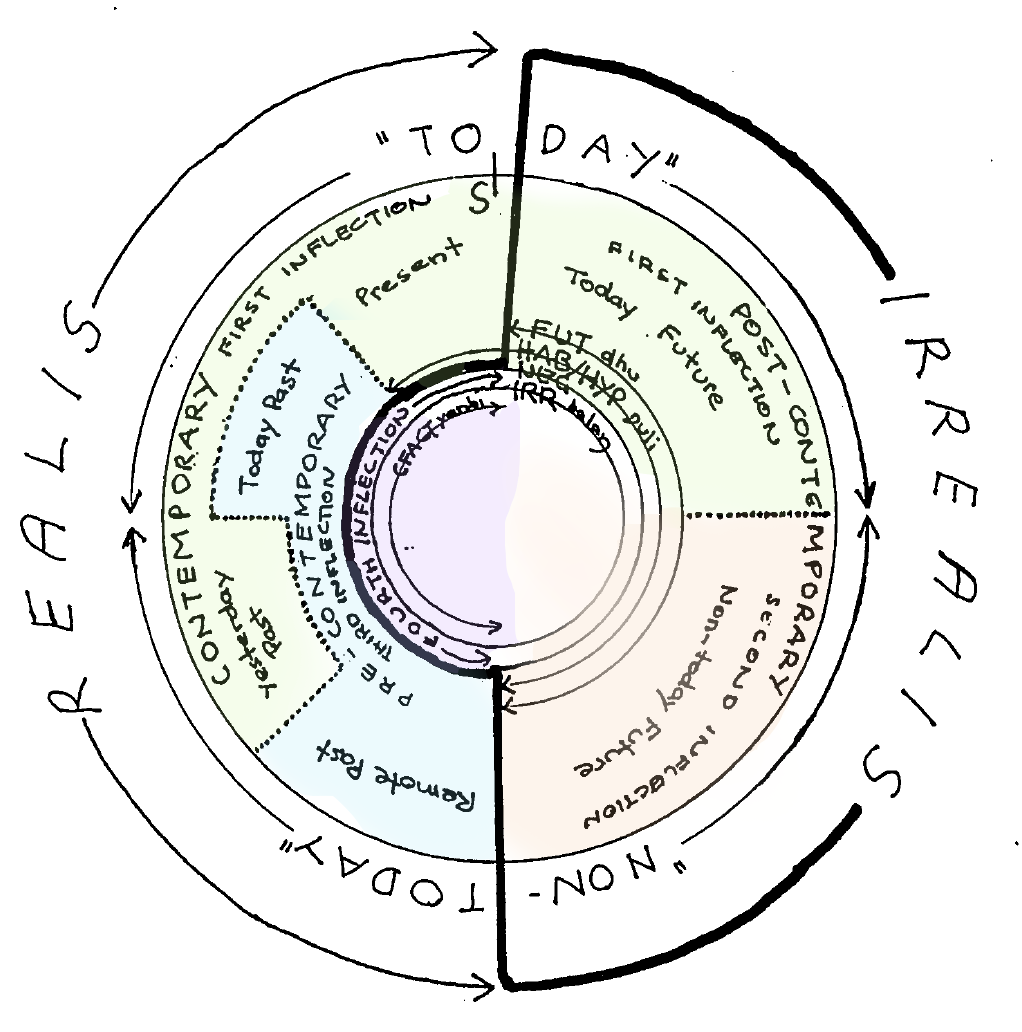
\includegraphics[width=0.85\textwidth]{WilkinsonDiagram362Col}
\end{figure}

Chapter \ref{yol-bkgd} provides background on Yolŋu Matha and the morphology of these languages' verbal paradigms, orienting the discussion around connections between temporal and modal concepts (particularly intention, prediction and futurity) and notions of relative grammatical ``prominence'' of tense, mood and aspect \citep[\textit{cf.}][]{Bhat1999}. %Subsequent chapter(s) focus on a number of morphosemantic phenomena (namely ``cyclic tense'' and ``asymmetric negation'') in the ``Western Dhuwal'' varieties of Yolŋu Matha, in view of providing an account of the semantics of the inflectional categories.



Subsequently, data further demonstrating the the expression of temporomodal distinctions and the interpretive intricacies of WD's paradigm semantics, focussing on a number of morphosemantic phenomena in Western Dhuwal(a) are provided in chapters \ref{sec:djr-temp} and \ref{sec:yol-mood} below. 

In light of these data, in chapter \ref{anY}, I propose a formal treatment of the paradigm on the basis of two semantic features: a temporal one -- \textsc{\textit{non-final instantiation}} -- and a modal one -- \textsc{\textit{metaphysical nonveridicality}}. As we will see, the notion of \textbf{branching times} ---introduced in chapter \ref{IntroCh} and deployed in the analysis of \textit{bambai} (ch. \ref{bambai.semx}) --- permits for a motivated, unified account of the ostensibly disparate sets of usage contexts that license each of \gls{wd}'s four inflectional categories. The essay concludes by considering the landscape of semantic variation across varieties of Yolŋu Matha, suggesting that the \gls{wd} system has arisen as a consequence of reanalysis and contact-induced meaning change.

\chapter{Background}\label{yol-bkgd}

\section{Grammars of TMA: the notion of ``prominence''}

In a \citeyear{Bhat1999} monograph, \citeauthor{Bhat1999} posits a typological parameter along which languages variably assign prominence to \textsc{tense, aspect \textup{or} mood}. For Bhat, determining which of these grammatical macrocategories a given language appears to assign ``prominence'' gives rise to a number of generalisations about characteristics of that language's grammar (``correlatable characteristics''). In particular, he suggests that, in a language where $ \mathcal C $ is given grammatical prominence, notions belonging to the other two categories tend to be ``viewed in terms of $ \mathcal C $'' (7).


An important consequence of this typology, in which languages can be classified and differentiated on the basis of these three broad types, is the implication that languages can ``move between them'' --- that is observable, synchronic variation across this parameter points to a history of reanalysis of, for example, temporal categories as modal ones. While Bhat does not explore this consequence of his typology in detail, he does point to observations in the grammaticalisation literature that have demonstrated ``cross-categorial change'' --- that is, situations where lexical material denoting some temporal, modal or aspectual category come to be reanalysed conveying meaning about a category in another semantic domain. Bhat suggest, for example, that the well-attested alternative grammaticalisation trajectories described by \cite{Bybee1994} (among others) and represented in Figure \ref{ta-gram} are determined by the ``prominence'' that a given language accords to either temporal or aspectual distinctions \citeyearpar[182]{Bhat1999}. Of course, this treatment to some degree begs the question. In a given pair of related languages, what is it that underpins the change from, \textit{e.g.}, perfect marking to perfective marking for $ \mathcal L_1 $ versus past-tense marking in $ \mathcal{L}_2 $?

\begin{figure}[h] \caption{Two examples of attested meaning change between the aspectual and temporal domains}\centering\label{ta-gram}

\begin{subfigure}[t]{.45\textwidth}\centering
		\begin{tikzpicture}[baseline=5pt]
		\draw  (0,0) node(pf)  {\textcolor{forest}{\textsc{perf}}};
		\draw (1.75,.5) node(pv) {\textsc{pfv}};
		\draw (1.75,-.5) node(ps)  {\textcolor{red}{\textsc{pst}}};
		\draw[thick,->] (pf) -- (ps);
		\draw[->] (pf) -- (pv);
	\end{tikzpicture}

\caption{\gls{perf} grams develop into \gls{pfv} markers (\citealp[e.g.][]{Condoravdi2014} for Indo-Aryan) or \gls{pst} markers (\citealp[e.g.][]{Schaden2012} a.o.)}
		\end{subfigure}\hfill
\begin{subfigure}[t]{.45\textwidth}\centering
		\begin{tikzpicture}[baseline=5pt]
		\draw  (0,0) node(pg)  {\textcolor{forest}{\textsc{prog}}};
		\draw (1.75,.5) node(ip) {\textsc{ipfv}};
		\draw (1.75,-.5) node(pr)  {\textcolor{red}{\textsc{pres}}};
		\draw[->] (pg) -- (ip);
		\draw[thick, ->] (pg) -- (pr);
	\end{tikzpicture}\caption{\gls{prog} grams develop into \gls{ipfv} markers (\citealp[see][]{Deo2015a}) or \gls{pres} markers (\citealp[e.g.][]{Heinrichs2002} for Neo-Aramaic)}
		\end{subfigure}
%\begin{tikzpicture}
%	content...
%\end{tikzpicture}
\end{figure}

\subsection{Futurity and mood-prominence}
Bhat marshalls data from Tibeto-Burman to show that ``mood-prominent'' languages have a tendency to grammaticalise a \textsc{future/nonfuture} distinction. He points in particularly to Manipuri ([\gls{mni}] Tibeto-Burman: Manipur), where this tense distinction appears to have ``developed from an earlier realis-irrealis modal distinction'' \citeyearpar[19]{Bhat1999}. Semantic connections between modal and future concepts are further suggested by frequently-attested semantic change pathways between, for example, expressions of intention and obligation (\textit{sc.} bouletic/deontic necessity) and futurity \citep[and then to epistemic modality, \textit{e.g.},][]{Bybee1978,Bybee1991,Bybee1994,Kuteva2019}.\footnote{\citet*{Bybee1991} hypothesise that the ``age'' of a future marker (\textsc{FutAge}) can be assessed in view of its semantic domain. In effect this amounts to a ``pathway'': $\textsc{deontic}\to\textsc{circumstantial}\to\textsc{future}\to\textsc{epistemic}$ \textit{etc.}} In her account of the diachrony (and ``instability'') of future expression in Romance, for example, \citet[31, 75, 106]{Fleischman1982} claims that as future markers become ``more temporalized'' (which she connects to their agglutination), functional pressure to recruit novel modal constructions emerges --- an early conceptualisation of a grammaticalisation cycle/``spiral.''
	%
	%The verbal suffix \textit{-le} is a future tense marker in Manipuri [\gls{mni}], whereas \citet[67ff]{Bhat1999} shows that in related Mao Naga [\gls{nbi}], it encodes irrealis modality, occurring in a number of modal, counterfactual and evidential constructions.
	%
	%\pex\a\begingl\gla \rightcomment{[Mao Naga]}alemono ovo hrü \textbf{le}-\textsc{t}i-e//
	%\glb Alemo pig buy \textbf{\gls{irr}}-\textsc{relevant}//
	%\glft`Alemo wanted to buy a pig (but couldn't as there was no money).'//\endgl
	%\a\begingl\gla pfo ico avuo bu \textbf{le}//
	%\glb he now meal take \textbf{\gls{irr}}//
	%\glft`He must be taking his meal now.'//\endgl
	%\xe


As suggested in \S~\ref{BT-review}, going back to Aristotle, it is well understood that the future has a dually temporal and modal character. That is, the truth of a future predication has frequently been analysed as changing with the passage of time --- that is ```future contingent'' statements can be neither true nor false' \citep[265]{Thomason1970}. Consequently, utterances about the future are often associated with predictive illocutionary force (this was a major theme guiding the analysis in part \textbf{\ref{bambai}}).

Consequently, contemporary formal treatments often embrace a modal semantics for ``future'' operators: one that departs from the earlier, priorian tense logic type approaches where truth is defined relative to time and --- the mirror image of \textsc{past} --- \textsc{future} is a sentential operator that serves to locate their prejacent subsequent to evaluation time.\footnote{Of course, as discussed in \S~\ref{BT-review}, Arthur Prior was crucially concerned about this asymmetry between the future and the past, over the course of his career he departing from an earlier belief in determinism and developing branching time models concerned with the indeterminate nature of the future. (\citealp[see][]{Copeland2020} and also \citealp[13]{Copley2009}).
	
	Generally speaking, on a deterministic view of the future, future morphemes can be unuderstood to universally quantify over an epistemic modal base (``possible candidates for the (preordained) future as far as I'm concerned'', \citealp[\textit{cf.}][]{Giannakidou2018}), whereas on non-deterministic views they quantify over a metaphysical modal base (``possible futures consistent with assumptions about metaphysical facts governing the world.'')} Modal accounts of future, then, often tend to take future-oriented morphology to universally quantify over a modal base. \citet[274]{Thomason1970} proposes a ``supervaluation''-based semantics for future-tensed predication as follows:\footnote{This following Copley's \citeyearpar[14]{Copley2009} conversion of \citeauthor{Thomason1970}'s account based on ``histories'' (which effectively imply sets of historical alternatives) into an equivalent one that speaks in terms of possible worlds. Thomason himself develops $ \mathcal{T\times W} $ frames in a \citeyear{Thomason1984} paper. See also \S\ref{BT-review} and \citep{Stojanovic2014} for discussion and an overview of different semantic approaches to the ``future contingents'' problem.}
\pex $ \denote[w,t]{\textsc{fut }p}=\left\{\begin{gathered}\begin{aligned} 1&\leftrightarrow &&\forall w'\big[w'\approx_t w \to\exists t' [t\prec t' \wedge p(w')(t')]\big]\\
0&\leftrightarrow &&\forall w'\big[w'\approx_t w \to\nexists t' [t\prec t' \wedge p(w')(t')]\big]
\end{aligned}\\
\text{undefined otherwise}\end{gathered}\right.
$\\[.5em]
\textsc{fut} $p$ is true if there's a time $ t' $ in the future of all metaphysical alternatives to $ w $ at $ t $ which $ p $ holds and false if there is no such time.\xe

\noindent As described earlier in this dissertation, $\cap\!\approx_t\!w $ represents the ``historical alternatives to $ w $ at $ t $'' (an equivalence class of worlds with identical histories to $ w $ up to $ t $) --- in effect equivalent to a \textit{metaphysical conversational background} (see \S~\ref{BT-review}.)


 Given how central this metaphysical assumption will be to the analysis, the approach taken by this chapter recasts this possible worlds formalism in terms of branching futures/times models. As in chapter \ref{bambai.semx}'s treatment of the distribution of \textit{bambai}, this will hopefully allow us to perspicaciously cash out the distinctions between the domains of \textsc{real} and \textsc{nonreal} eventualities. That is, a metaphysical conversational background $ \cap\!\approx_i $ will be representable by an equivalence class of branches, undivided until $ i $, that represent metaphysically possible developments of the world from $ i $.

\subsection{Negation and mood}\label{sec:asymneg}

Developing a broad cross-linguistic typology of sentential negation, \citet[208]{Miestamo2005} proposes a class of languages (\textsc{a/nonreal}) which have `grammaticalized the fact that negation belongs to the realm of the non-realized' --- that is, negative and modal operators are shown to interact formally in a number of ways. According to Miestamo, ``asymmetric negation'' phenomena are notably overrepresented in the languages of Australia (and to a lesser extinct New Guinea, driving him to describe \textsc{a/nonreal} as a ``circumpacific phenomenon'' (192, 411)). \citet[\S2.2]{Phillips2021b} provides an overview of a number of mood-based asymmetry phenomena in Australian languages.


For many languages, \textsc{a/nonreal} is manifested as the \textbf{neutralisation} of a grammatical distinction between \textsc{realis} and \textsc{irrealis} modalities in negative clauses. That is, ±\textsc{realised} is associated with a a morphosyntactic distinction in positive clauses that is not available in negative ones. Shown in the Gurrgoni (\gls{gge}, Maningrida: Arnhem) data in (\getref{sn-gvg}), a reality status distinction is morphologically realised in positive clauses (\getref{sn-gvg.rea}-\getref{sn-gvg.irr}) which is not available to its negative counterpart (\getfullref{sn-gvg.neg}), which is obligatorily irrealis-marked and ambiguous between a modal and non-modal reading. As we will see below, a similar phenomenon is exhibited in some varieties of Yolŋu Matha (notably those varieties closer to Maningrida.)


	\pex\deftagex{sn-gvg}
\textbf{Interactions between negation and mood marking in Gurrgoni} 
\iffalse	\a\begingl\glpreamble present-tensed //
\gla dji-na-ni wurrparn//
\glb 3s/3o-see-\textsc{precontemp} emu//
\glft `They didn't see an emu'//\endgl b.\quad\begingl\glpreamble neg present-tensed //
\gla galu dji-na-djirni djit-bolupu nuyu//
\glb \textsc{neg} 3s/3o-see-\textsc{irr} 3s-mother  //
\glft text//\endgl \fi

\a\begingl\glpreamble Past-tensed (nonmodal)\deftaglabel{rea}//
\gla nji-weki-\textbf{ni}//
\glb 2s-talk-\textsc{precontemp}//
\glft `You talked.'//\endgl \a\begingl\glpreamble Past-tensed (modalised)\deftaglabel{irr}//
\gla nji-weki-\textbf{yarni}//
\glb 2s-talk-\textsc{\textbf{irr1}}  //
\glft `You might have talked.'//\endgl	\a\begingl\glpreamble Negative past-tensed\deftaglabel{neg}//
\gla galu nji-weki-\textbf{yarni}//
\glb \textsc{neg} 2s-talk-\textsc{\textbf{irr1}}  //
\glft `You didn't/mightn't have talked.'\trailingcitation{(adapted from \citealp[307]{Green1995})}//\endgl


\xe



Irrealis markers are broadly taken to realise semantic operators which displace the instantiation of a given eventuality into the realm of the nonrealised. Relatedly, negative operators indicate the \textsc{nonrealised} status of some predicate.

Consequently, for languages exhibiting \textsc{a/nonreal}, irrealis and negative operators can be thought of as performing conceptually-related functions. \citep[see also][208]{Miestamo2005}.

 It is on these functional grounds that negation and mood interact; predicting parametric variation across languages.

%todo asymmetry. Muna participates (Bhat 67)


%\subsection{The semantics of a mood-based inflectional system}

\section{Yolŋu Matha}

%Class of YM was discussed in Ch..... 
%To reorient the reader.....
%Djr, Wag are related....
%could move post-defense
Yolŋu Matha is a small language family spoken in North-Eastern Arnhem Land, in the Northern Territory of Australia (map provided in \ref{map}, see also discussion in \S~\ref{sec:ecol}). The family is a subgroup of the larger Pama-Nyungan family, representing something of an enclave in Northern Australia; surrounded by a diversity of unrelated languages.

\begin{figure}[h]
	\centering\caption{Traditional language communities in Northern Australia \citep{Horton1996}.Yolŋu Matha is the gold coloured area within the square in the primary map.\\\textbf{Inset. }Northeast Arnhem land (colourised from \citealt[2]{Wilkinson1991}. Yellow shading indicates the \textit{Yolŋu Wäŋa} (homeland). Brown and green circles indicate the contemporary distribution of Yolŋu languages investigated. Purple circling indicates the neighbouring (but genetically unrelated) Maningrida language family.}	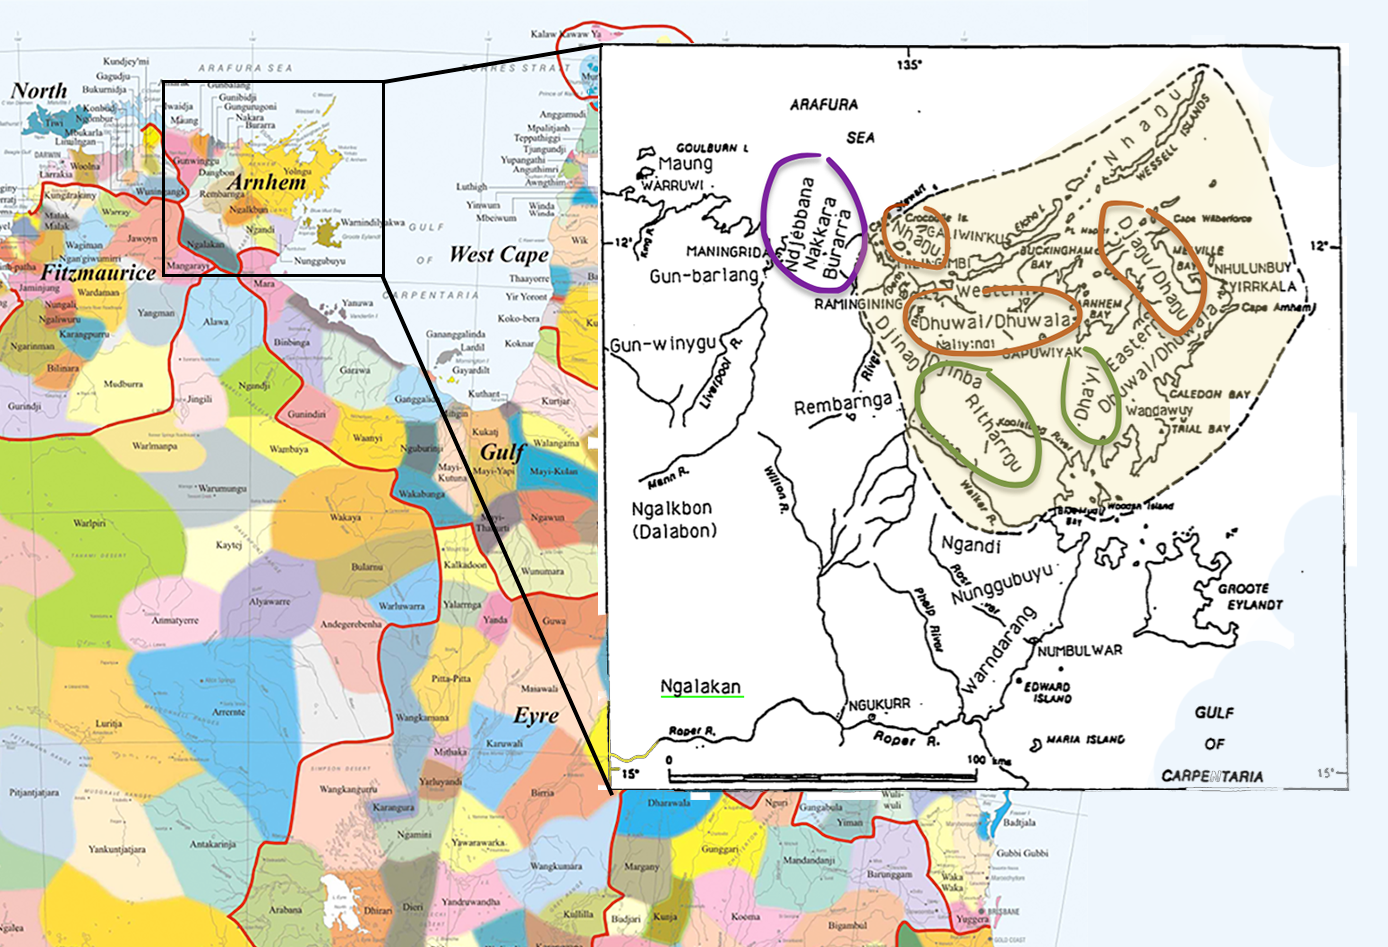
\includegraphics[width=0.9\textwidth]{AustralianLangsCropped.png}\label{map}
\end{figure}


Most Yolŋu linguistic phylogenies posit a high-level split between Western, Northern and Southern subgroups. This is schematised in Figure \ref{YM-phylo}. Yolŋu society is traditionally organised according to a moiety system --- that is, the Yolŋu universe is organised into two ranging sets, \textit{Yirritja} and \textit{Dhuwa} --- and continues to be strictly exogamous with respect to moiety. Given that each Yolŋu clan is associated with a single patrilineal moiety and corresponding language variety, households are necessarily multidialectal, one member of a couple speaking a \textit{Yirritja} lect, the other speaking a \textit{Dhuwa} lect. Children inherit their father's moiety (and language), and marry into their mother's moiety \citep[see also][62\textit{ff}]{Williams1986}. This chapter focuses primarily on a number of Southern Yolŋu varieties (see Fig \ref{DDvars}). 


\begin{figure}
\caption{A broad phylogenetic classification of Yolŋu subgroups, following \citealt{Wilkinson1991,Schebeck2001,Waters1989} a.o.}\centering\label{YM-phylo}
	\begin{tikzpicture}\tikzset{edge from parent/.style=
{draw,
edge from parent path={(\tikzparentnode.south)
-- +(0,-8pt)
-| (\tikzchildnode)}}}
		\Tree  [.\textbf{Yolngu~Matha} [.\textsc{Western} [.Djinang ] Djinba ] [.\textsc{Northern} Nhaŋu Dhaŋu-Djaŋu ] [.\textsc{Southern} \textit{Fig~\ref{DDvars}} ] ]
	\end{tikzpicture}
\end{figure}

\begin{figure}[h]\centering	\caption{Varieties (`clanlects'/dialects) of \textcolor{teal}{Dhuwal}-\textcolor{ochre}{Dhuwala} in the context of the Southern Yolŋu languages \citep[following][13]{Wilkinson1991} with some adaptation following \citet[15]{Schebeck2001}.}\label{DDvars}
	\begin{tikzpicture}[every node/.append style={align=right},every tree node/.style={anchor=north}]
		\Tree [.\textsc{\textbf{Southern~Yolŋu}} [.\textbf{\textcolor{ochre}{Ritharrŋu}-\textcolor{teal}{Wägilak}} $\vdots$ ] [ [.\textbf{Dhay'yi} $\vdots$ ] [.\textbf{Dhuwal-Dhuwala} [.\textsc{western} \node[text=teal,font=\itshape]{\bf\it Djambarrpuyŋu\\Ḻiyagalawumirr\\Ḻiyagawumirr\\Marraŋu\\$ \vdots $}; \node[font=\itshape,text=ochre]{\bf\it Gupapuyŋu\\Wubulkarra\\$ \vdots $}; ]   [.\textsc{eastern} \node[font=\itshape,text=teal] {\textbf{Djapuˀ}\\Marrakulu\\Ḏäṯiwuy\\$ \vdots $}; \node[font=\itshape,text=ochre]{\textbf{Gumatj}\\Maŋgalili\\Munyuku\\Maḏarrpa\\$ \vdots $}; ] ] ] ]
	\end{tikzpicture}
	
\end{figure}\marginnote{right this is the classification in Wilk 91 which follows Dixon 80 presumably? Claire's phylogeny is different in a number of ways. how to handle?}

As indicated in the diagram, the \textit{Dhuwal} and \textit{Dhuwala} groupings effectively represent the distinct clan-lects of a single speech community --- associated with \textit{Dhuwa} and \textit{Yirritja} moieties respectively. Incidentally, \citet{Wilkinson1991} points out that the degree of similarity between Western Dhuwal and Dhuwala are more closely related to one another than either is to Eastern Dhuwal and Dhuwala (I assume that this fact is representable phylogenetically and has been represented in Figure \ref{DDvars}). A (the?) primary distinction between Dhuwal and Dhuwala varieties cross-cutting the language area results from a productive apocope rule (investigated in \citealp{Morphy1977}, \citealp[see also][94\textit{ff}]{Wilkinson1991} for further details.). The formal consequences of Dhuwal apocope on the verbal paradigm are partially indicated in parentheses in Table \ref{djr-pdm-exx} below. The table gives examples of the verb paradigm for each of the major Djambarrpuyŋu conjugation classes as described by \citet[306\textit{ff}]{Wilkinson1991} (parentheses give the corresponding verb group number assigned by \citealt{Lowe1996} for Gupapuyŋu.)


%\section{Dhuwal-Dhuwala: Djambarrpuyŋu \& Gupapuyŋu}\label{djr}
\section{The Yolŋu verb: Typology \& morphosemantics}\label{yol-paradigms}

With the exception of the Western Yolŋu varieties \citetext{\textit{i.e.}, Djinaŋ \& Djinba, see \citealp{Schebeck2001,Waters1989}}, Yolŋu varieties are largely mutually intelligible \citep{Heath1981b,Morphy1983}. Yolŋu languages have a verbal paradigms which are at least partially cognate and likely reconstructable to a proto-system \citetext{\citealp{Schebeck2001}, \citealp[see comparative reconstruction pilot work by ][]{Bowern2009}.} All varieties have between three and six different inflectional classes; each inflection is responsible for encoding (combinations of) temporal (tense/aspect) and modal information --- as described above, it is the semantics of these inflections with which we will be primarily concerned in this dissertation. The forms of each inflection additionally varies depending on the conjugation class associated with a given verb stem (or derivational suffix) --- authors of descriptions of various Yolŋu varieties having identified between three \citetext{\citealp[\textit{e.g.},][]{Waters1989} on Djinba \& Djinba} and nine \citetext{\citealp[\textit{e.g.},][]{Lowe1996} on Gupapuyŋu} distinct conjugation classes.

In view of demonstrating the structure of a Yolŋu verbal paradigm, in this section, I present a brief overview of the morphosemantics of the range of inflectional classes in Wägilak --- the southernmost variety of Yolŋu Matha and a close relative of Dhuwal --- on the basis of new data elicited in the field, in addition to \citeauthor{Heath1980r}'s \citeyearpar{Heath1980r} description of Ritharrŋu.\footnote{Many thanks to Salome Harris for collecting questionnaire-data from Wägilak and Ritharrŋu in Ngukurr, mid-2019.}

\subsection{The Ritharrŋu-Wägilak paradigm}\label{sec:rit.paradigm}

According to \citet[60--75]{Heath1980r}, the Ritharrŋu (Wägilak) verbal paradigm distinguishes six main conjugation classes which, each of which marks four inflectional categories. These inflections establish a three-way tense distinction between the \textcolor{blue}{\textsc{past}}, \textcolor{forest}{\textsc{present}} and \textcolor{ochre}{\textsc{future}}. He describes the fourth category as the \textcolor{purple}{\textsc{past potential}}, supplying data of the latter's use in counterfactual situations. The paradigm is represented by table \ref{rit.paradigm}, while the data in (\ref{wag-infls}) demonstrates the (straightforward) temporal semantics of each of these inflectional categories.


\begin{table}[h]\caption{Examples of conjugation patterns for the Ritharrŋu-Wägilak verbal paradigm \citep[adapted from][63--6]{Heath1980r}}\label{rit.paradigm}\small
	\begin{tabular}{>{\bf}l>{\sc}l>{\it}l>{\it}l>{\it}l>{\it}l}\toprule
		\textsc{class} & \textsc{stem} & \textcolor{forest}{\gls{pres}} & \textcolor{ochre}{\gls{fut}} & \textcolor{blue}{\gls{pst}}\footnotemark & \textcolor{purple}{\gls{cfact}}\\\midrule
		1 & `go' &	wäni & wäni & wäni-\textbf{na}/-\textbf{nya} & wäni-\textbf{ya}\\
 2& `eat' & ḻuka & ḻuk-\gls{I} & ḻuka-\textbf{nha}& ḻuk\textbf{-iya}\\
 3& `chase'& ŋupa& ŋupa-\textbf{ru}&ŋupa-\textbf{na} &ŋupa-\textbf{ra} \\
 4&`hold' & gatha-\textbf{ŋ} &gaṯu-\textbf{lu} &gatha-\textbf{(la)ra} & gatha-\textbf{la} \\
 5&`push' &djaranydju\textbf{-n} &djaranydju\textbf{-ru} &djaranydju\textbf{-na} &djaranydju\textbf{-ra} \\
 6\textsc{b}&`protect' &gunga\textbf{-ma} & gungu\textbf{-ŋu}& gunga\textbf{-wala/-nha} & gunga\textbf{-wa}\\\bottomrule
	\end{tabular}
\end{table}
\footnotetext{Where there are two forms given for the \textcolor{blue}{\gls{pst}} marker, \citet{Heath} is ambivalent about the semantic characteristics of each form --- i.e., whether they are synonymous or whether they represent a defective distinction. We will provide further evidence for the latter persepctive in \S\ref{yol-change}.}



\pex \textbf{The temporal interpretation of each inflectional class in Wägilak}\label{wag-infls}
\a\begingl\gla \rightcomment{\textcolor{forest}{\textbf{[\textsc{present}]}}}\textbf{nhäma} rra yakuthi mukulnha//
\glb see.\textbf{{\I}} 1s now aunt.\textsc{acc}//
\glft`I'm (not) looking at my aunt currently.'\trailingcitation{[RN~20190520]}//\endgl\deftagex{wag-pres}\
\a\begingl\gla \rightcomment{\textcolor{ochre}{\textbf{[\textsc{future}]}}}goḏarrpuy ŋarra \textbf{nhäŋu} mukulnha//
\glb tomorrow 1s see.\II{} aunt.\textsc{acc}//
\glft`I will (not) see my aunt tomorrow.'\trailingcitation{[DW~20190522]}//\deftagex{wag-fut}\endgl
\a\begingl\gla \rightcomment{\textcolor{blue}{\textbf{[\textsc{yesterday past}]}}}ripurru-mirri ŋarra \textbf{nhäwala} mukulnha//
\glb yesterday 1s see.\textbf{\III} aunt.\textsc{acc}//
\glft`I saw (didn't see) my aunt yesterday.'\trailingcitation{[RŊ~20190522]}//\endgl\deftagex{wag-pst}
\xe

\noindent Further, (\getref{rit.mods}) shows the modal uses of \gls{fut} and \gls{cfact} inflections. In (\getfullref{rit.mods.a}-\getref{rit.mods.imp}), \II~is compatible with a number of modal (\textit{e.g.}, deontic, conditional) readings, including in imperative utterances. Similarly, \gls{cfact} is compatible with a range of ``modal-for-the-past''/counterfactual readings, as shown by Heath's translation in (\getfullref{rit.mods.cf}).


\pex \textbf{The \textsc{future} and \textsc{past potential/counterfactual} in modalised contexts in Ritharrŋu-Wägilak}\deftagex{rit.mods}
\a \begingl\gla blijiman ŋay waŋa-na: ``gulu-\textbf{rru} nhe yiŋ'-ŋiri\textdblhyphen{dhi} wäŋa-ya. Yakaŋu nhe \textbf{wäni}-'may garra nhe git lokdap-\textbf{urru}"//
\glb policeman 3s say-\III~ stay-\II~ 2s \gls{dist}-\gls{loc}\textdblhyphen\gls{foc} home-\gls{prom} \gls{neg} 2s go.\II-\gls{neg} \textit{garra} 2s \textit{get} locked.up-\II//
\glft`The policeman said you must stay here at home. Don't go (anywhere) or you'll be locked up.'\trailingcitation{[RŊ~20190520~18']}\deftaglabel{a}//\deftagex{wag-pot}\endgl
\a\begingl\gla \textbf{wäni} nhe//
\glb go.\II~ 2s//
\glft `You can/should/will go.' (or `Go!')\trailingcitation{\citep[104]{Heath1980r}}\deftaglabel{imp}//\endgl
\a\begingl\gla wäni\textbf{-ya} nhe//
\glb go-\V~ 2s//
\glft`You could/should/would/were about to go.'\trailingcitation{\citep[104]{Heath1980r}}\deftaglabel{cf}//\endgl
\xe

This distribution can be straightforwardly represented by appealing to the ``modal trichtomy'' \citetext{\textit{cf.} \citet{VonPrince2019,VonPrincea} --- introduced in \S \ref{vP-trich}, compare (\getref{trichot}), \textit{p.}~\getref{vP-bt0}.} Effectively, Ritharrŋu-Wägilak's four inflections can be thought of as a partition of a branching-time. This is shown in (\nextx) and schematised in Figure \ref{rit-BT}.


\pex \textbf{Domains of the four inflections in Ritharrŋu-Wägilak, given a branching time frame $ \mathfrak U =\langle\mathcal I,\prec\rangle$ and an evaluation index $ i* $}


\denote[i*]{\gls{pres}}  : \textsc{actual present} $ \{i\mid i = i*\} $\\
\denote[i*]{\gls{fut}}  : \textsc{potential} $ \{i\mid i \succ i*\} $\\
\denote[i*]{\gls{pst}}  : \textsc{actual past} $ \{i\mid i \prec i*\} $\\
\denote[i*]{\gls{cfact}}  : \textsc{counterfactual} $ \{i\mid \langle i,i*\rangle\text{ is unordered by }\prec\} $
\xe

\begin{figure}[h]
	\caption{Ritharrŋu-Wägilak's verbal paradigm partitions the branching frame/modal domain (modelled as a set of partially-ordered indices.)}\label{rit-BT}\centering
	\begin{tikzpicture}
		[scale=2.5,level distance=9mm,
		every node/.style={fill=purple,circle,inner sep=1.5pt},
		level 1/.style={nodes=purple,sibling distance=10mm},
		level 2/.style={sibling distance=8mm},
		level 3/.style={sibling distance=4mm},
		level 4/.style={sibling distance=2mm},
		edge from parent/.style={draw,thick}]
		\node[color=blue,minimum size=2mm] {} [grow=right]
		child {node {} edge from parent[densely dotted,color=purple]
			child {node {}
				child {node {}
					child {node {}}
					child {node {}}}
				child {node {}
					child {node {}}
					child {node {}}}}
			child {node {}
				child {node {}
					child {node {}}
					child {node {}}}
				child {node {}
					child {node {}}
					child {node {}}}}}
		child[missing]
		child {node[color=blue,minimum size=2mm] {}
			child {node {} edge from parent[densely dotted,color=purple]
				child {node {}
					child {node {}}
					child {node {}}}
				child {node {}
					child {node {}}
					child {node {}}}}
			child {node[color=purple] {} edge from parent[densely dotted,color=purple]
				child {node {}
					child {node {}}
					child {node {}}}
				child {node {}
					child {node {}}
					child {node {}}}}
			child {node [style={fill=forest,minimum size=4mm},label=above:$ \boldsymbol{{\color{gray!95}i*}} $] {} []
				child {node[fill=ochre] {} edge from parent[densely dashed,color=ochre,every child=every node\.style={fill=ochre,circle,inner sep=1.5pt}]
					child {node[fill=ochre] {}}
					child {node[fill=ochre] {}}} 
				child {node[fill=ochre] {} edge from parent[densely dashed,color=ochre]
					child {node[fill=ochre] {}}
					child {node[fill=ochre] {}}}} };
	\end{tikzpicture}
\end{figure}


As an example then, the contribution of \textcolor{forest}{\gls{pres}} (following standard assumptions about tense) is taken to be the restriction of a given predicate (\textit{P})'s instantiation to actual indices that overlap with the present: \textit{i.e.}, \gls{pres}(\textit{P}) is true iff \textit{P} is instantiated at $ i* $.

\subsection{The central Arnhem linguistic area}
This section has so far sought to familiarise the reader with the basic structure of a Yolŋu Matha verbal paradigm, taking the example of the Ritharrŋu-Wägilak (Southern Yolŋu) variety. 

In the sections that follow, we turn to a description of the distribution of the inflectional categories in Western Dhuwal-Dhuwala (\gls{wd}). As we will see (and as shown in the introduction to this part of the dissertation), there are a number of phenomena that complicate a unified treatment of the semantics of the \textsc{wd} paradigm. Introduced above, these phenomena include a \textsc{cyclic tense} system and \textsc{asymmetric negation}.


Importantly, these phenomena are not exhibited in most Yolŋu lanuages, including those varieties phyletically closest to \textsc{wd}, \textit{viz.} Ritharrŋu-Wägilak as well as the Eastern (\textit{``Miwatj''}) varieties of Dhuwal-Dhuwala centered around Yirrkala (compare figures \ref{YM-phylo} \& \ref{DDvars}.) Similar patterns are, however, characteristic of the languages of Maningrida --- Burarra, Gurrgoni, Nakkara and Ndjébanna. Varieties of Djinaŋ (a Western Yolŋu outlier) are spoken in the Maningrida community and its outstations. The Ramingining community --- traditionally the land of the Ganalbingu tribe (a \textit{Yirritja} Djinba moiety) --- is approximately 100km east of Maningrida. Djinaŋ, Djinba and \gls{wd} (the westernmost varieties of Dhuwal-Dhuwala) all exhibit the cyclicity and asymmetric negation that is characteristic of the grammars of the Maningrida languages.

In view of the sustained contact between the non-Pama-Nyungan Maningrida languages and the (geographically) western varieties of Yolŋu Matha, it is assumed here that these two properties are examples of areal phenomena that characterise the languages of central Arnhem Land \citetext{see appendix 2 of \citealt{Waters1989} for a short investigation of this perspective.}


\begin{center}
	
\huge\sf	 ※
	
\end{center}


\noindent I will argue that these two phenomena --- \textit{cyclic tense} and \textit{asymmetric negation} (w/r/t reality status marking) --- are undergirded by the grammaticalisation of two semantical properties---\textsc{\textbf{non-final instantiation}} and \textsc{\textbf{nonveridicality}} respectively. These properties will be further precised and couched in a more detailed discussion of the expression of temporal and modal categories in \gls{wd} (chh.~\ref{sec:djr-temp}--\ref{sec:yol-mood}). A formal proposal (in terms of branching times) for the semantics of the \gls{wd} verbal paradigm is presented in chapter \ref{anY}.


%todo §§4.1-4 to migrate directly in as descriptive background chapters
\section{Verbal inflection in Western Dhuwal(a)}\label{djr-infl}

%\subsection{\gls{wd} Paradigm structure \& distribution of the inflections}\label{infls}

TMA distinctions in Western Dhuwal(a) are partially encoded in a paradigm that distinguishes four `inflections', which are cognate with a number proto-Yolŋu inflections according to the reconstructions provided by \citet{Bowern2009}. Unlike for Ritharrŋu-Wägilak, summarised above (\S~\ref{yol-paradigms}), work on Dhuwal-Dhuwala varieties---most notably Beulah \citeauthor{Lowe1996}'s notes and lessons on Gupapuyŋu (first published in 1960) and Melanie \citeauthor{Wilkinson1991}'s 1991 Djambarrpuyŋu reference grammar [republished \& cited here as \citealp{Lowe1996,Wilkinson1991} respectively]---has tended to eschew a metalinguistic gloss for these inflections, given the ostensible non-unifiability of their semantics:\footnote{Relatedly, in his treatment of Djinaŋ and Djinba, \citet{Waters1980,Waters1989} glosses the function-in-context of each inflection, perhaps implying a polysemy treatment of each inflection in these languages: ``[In Djinaŋ, t]here are twelve semantic categories for every verb, which are coded by seven suffixal forms. Consequently, five of the forms each code two different semantic categories...'' \citeyear[142]{Waters1980}} the distribution of each of these inflectional categories is discussed in greater detail in this section. In addition to these inflections, the labour of encoding temporal and modal relations in \gls{wd} is shared by a (closed) class of auxiliaries, which appear to interact with the verbal paradigm. 




Further complicating the exposition of this (and a feature across Yolŋu Matha varieties, see \S~\ref{yol-paradigms}), is the fact that there are a number of \textit{conjugation (sub)classes}: \citet{Lowe1996} enumerates nine classes. The (more detailed) description by \citet{Wilkinson1991} shows that these correspond to three larger conjugation classes --- the \textit{Ø-}, \textit{N}- and \textit{Ŋ-}classes --- each associated with a number of subclasses,\footnote{\citeauthor{Wilkinson1991} identifies 14 distinct inflectional patterns in addition to a ``non-inflecting'' class \citeyearpar[307]{Wilkinson1991}.} in addition to ``non-inflecting'' and (semi-)irregular categories \citep{Wilkinson1991}. The paradigm for six \gls{wd} verbs, taken to be representative of distinct different conjugation patterns is given in Table \ref{djr-pdm-exx}.

%todo\mcom{Of course I can provide more detailed information (the subclasses) but that feels like it'd be better appended? The comparative spreadsheet i've made/Claire's 2009 stuff has most of this formative data... \\\textbf{note: Andrea Simms strongly suggests more exposition of the formal paradigm} }
\begin{table}[h]
	\caption{Examples of the paradigm of four morphological TMA inflections in Djambarrpuyŋu [\gls{djr}] and (Gupapuyŋu [\gls{guf}] resyllabification in parentheses).\\{}[\gls{djr}] data and classification from \citet{Wilkinson1991}; [\gls{guf}] data and classification from \textit{Gupapuyŋu} \citeyearpar{Lowe1996}.} \label{djr-pdm-exx}
	\centering
	\begin{tabular}{rl|>{\it}l>{\it}l>{\it}l>{\it}l}
		\textbf{Class} & \textbf{\textit{Example}} & \textup{\I} & \textup{\II} & \textup{\III} & \textup{\IV}\\\midrule
		$\boldsymbol\emptyset_{i}$\hfill(2)& \textit{marrtji} `go' & \textit{marrtji}& \textit{marrtji} & \textit{marrtji\textbf{n(a)}} & \textit{marrtji\textbf{nya}}\\
		
		$ \boldsymbol\emptyset_{\textit{a}} $\hfill (3) & \textit{ḻuka} `consume' & \textit{ḻuk\textbf{a}} & \textit{ḻuk\textbf{i}} & ḻuka\textbf{n(a)} & ḻuka\textbf{nha}\\

		$\boldsymbol\emptyset_{\textit{rr}}$ \hfill (4)& \textit{waṉḏirr(i)} `run' & \textit{waṉḏi\textbf{rr(i)}}& \textit{waṉḏi} & \textit{waṉḏi\textbf{n(a)}} & \textit{waṉḏi\textbf{nya}}\\
		
		
		
		\textbf{N}\hfill(5)& \textit{ḻupthun} `wash' &\textit{ḻuphtu\textbf{n}} & \textit{ḻupthu\textbf{rr(u)}} & \textit{ḻupthu\textbf{rr(una)}} & \textit{ḻupthu\textbf{na}}\\
		
		\textbf{N$ _{L} $}\hfill(6)& \textit{gurrupan} `give' & \textit{gurrup\textbf{an}} & gurrupu\textbf{l(u)}&gurrupa\textbf{ra}& gurrupa\textbf{na} \\
		
		\textbf{Ŋ}\hfill(7)& \textit{nhäma} `see' & \textit{nhä\textbf{ma}} & \textit{nhä\textbf{ŋu}} & \textit{nhä\textbf{ŋal(a)}} & \textit{nhä\textbf{nha}}\\
	\end{tabular}
	
\end{table}


Above, I alluded to Beulah Lowe's eschewal of a ``semantic description'' for each of the four inflectional classes, also followed by Melanie Wilkinson. Throughout, these categories will be glossed with bold-faced Roman numerals, following the conventions established by Lowe (see also Table \ref{Infl-Comparisons-Wilk}, which adapts Wilkinson's summary of glossing decisions made by other grammarians.)% -- complex sentences and predications are investigated in further detail in §\ref{djr-subord}.

%Table \ref{Infl-Comparisons-Wilk}, adapted from \citet[336]{Wilkinson1991} summarises the metalanguage decisions made by other authors in their attempts to describe Dhuwal(a) varieties.

\begin{table}[h]
	\caption{Summary of metalinguistic descriptors deployed by a number of grammarians for the four inflectional classes in a number of Dhuwal/Dhuwala varities, adapted from \citet[336]{Wilkinson1991}.}\label{Infl-Comparisons-Wilk}\small
	\begin{tabular}{lr|llll}
		&&	\textbf{\I}	& \textbf{\II}	&	\textbf{\III}	&	\textbf{\IV}\\\midrule
		\citealt{Wilkinson1991}& \gls{djr} &\textsc{First}&\textsc{Second}&\textsc{Third}&\textsc{Fourth}\\
		\citealt{Lowe1996}\footnotemark &\gls{guf} &Primary&Secondary&Tertiary&Quartenary\\
		\citealt{Tchekhoff1983}& \gls{djr}&\textsc{Bas}e&\textsc{Fut}ure&Past\textsubscript1&Past\textsubscript2\\
		\citealt{Heath1980}& \gls{dwu} & Pres/Fut & Fut/Imp & Past & Past Remote\\
		\citealt{Morphy1983}& \footnotesize Djapuˀ & Unmarked & Potential & Perfective & Past Non-indicative\\
	\end{tabular}
	
\end{table}	\footnotetext{\Citealt{VanderWal1992} adopts the same labelling scheme as \citet{Lowe1996} although her analysis of the distribution of each of Gupapuyŋu's inflectional classes seems to diverge somewhat from \citeauthor{Lowe1996}'s.}

 In the following subsections, I provide examples of the functional domains of each of the four inflections in Western Dhuwal-Dhuwala and other lexical material relevant to encoding TMA relations in this language.

%todo MW diagram is now in the intro to this subpart
% Figure \ref{WilkDia} comprises a (colourised) reproduction of \citeauthor{Wilkinson1991}'s schematisation of the functional domain and collocation features of each Djambarrpuyŋu inflection. Data exemplifying the distribution of WD's four inflectional categories is provided in the subsections below in conjunction with a discussion of the approximate range of each.
%
%\begin{figure}[h]\caption{Melanie Wilkinson's \citeyearpar[326]{Wilkinson1991} schematisation of the complex semantic space associated with each of the four inflectional categories in Djambarrpuyŋu. My colourisation.}\label{WilkDia}\centering
%	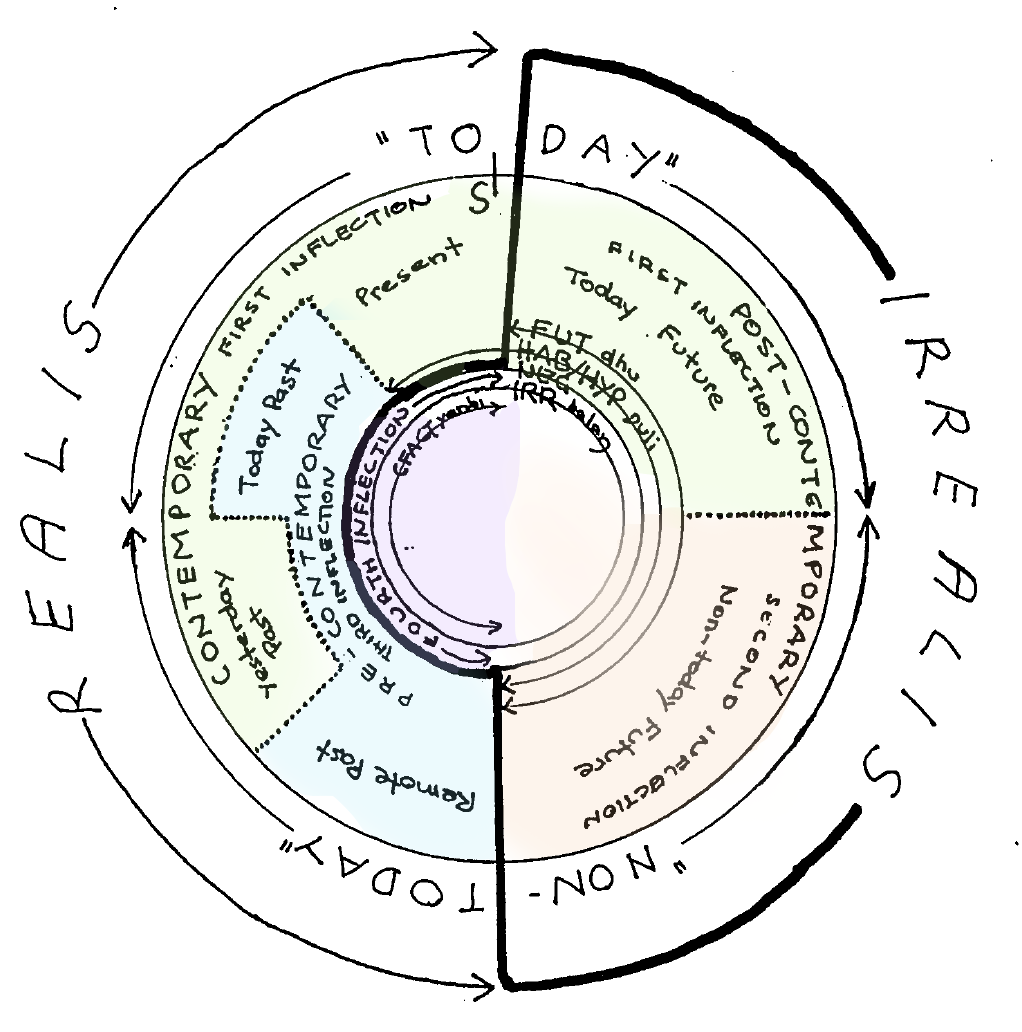
\includegraphics[width=0.8\textwidth]{WilkinsonDiagram362Col}
%\end{figure}

\subsection{The Primary inflection}\label{desc-i}

The `primary' inflection (\I), cognate with inflections in other Yolŋu languages which have been described as ``unmarked'' or ``base'', surfaces in predications that are interpreted with any of \textsc{present}, \textsc{past} or \textsc{future} reference. Here I provide examples of \I-inflected clauses receiving each of these temporal interpretations.

%\mcom{Now for both of these (and i suspect all sentences in this sssection) context ought to be modulable s.t. a non-present reading is available. This can/should/will be tested in the field}
\pex\textit{\textbf{ Present-reference encoded with \gls{I}}}

\a\begingl\deftagex{IPres}\deftaglabel{nhina}
\gla Ŋunhi-y ŋunhi ḏirramu \textbf{nhina} ga//
\glb \gls{texd}\textsc{-erg} \textsc{texd} man sit.\I{} \textsc{ipfv.\I}//
\glft`There that man is sitting.'\trailingcitation{\citep[856]{Tchekhoff1983}}// 
\endgl
%\a\begingl \gla ŋarra \textbf{marrtji}-n dhiyaŋu-n bala//
%\glb 1s go\textbf{.I}-\gls{seq} \gls{prox}.\gls{erg}-\textsc{seq} then//
%\glft`I am going now.'\trailingcitation{\citep[256]{Wilkinson1991}}//\endgl
\a\begingl\gla Ŋarra ga \textbf{ḻuka} gapu (dhiyaŋu bala)//
\glb 1s \textsc{ipfv.\gls{I}} consume.\gls{I} water \gls{texd}.\gls{erg} then//
\glft`I'm drinking water at the moment.'\trailingcitation{[DhG 20190405]}//\endgl
\xe

The sentences given in (\getref{IPres}) show the compatibility between present temporal reference and the \gls{I} inflection: in both cases, the event described by the predicate --- \textit{nhina} `sit.\gls{I}' and \textit{marrtji} `go.\gls{I}' --- is understood as contemporaneous with speech time. In each sentence, imperfective marking (\textit{ga} `\gls{ipfv}') is obligatory in order to establish present reference (see \S \ref{sec:djr-temp}).



In addition to those present-referring sentences in (\getref{IPres}), the data in (\getfullref{pstI}) show compatibility between \gls{I} and past time reference. In each of these examples, the events described by the predicates---\textit{e.g.}, the arrival event described by \textit{ŋayatham} in (\getfullref{pstI.ŋayatham})---\textit{precede} speech time. Similarly, the two past events in (\getref{pstI.rrupiya}) both receive \gls{I} inflection. The instantiation times of both of these events are further restricted (to the recent past) by temporal frame adverbs \textit{barpuru} $\approx$ `yesterday'. % -- frame adverbials of this type are discussed in some detail in §\ref{TFA}.

%\mcom{Is it a shitty idea to use colour coding for more formatting/highlighting options? I want to reserve bold for the verbforms themselves but would like to be able to second-order emphasise non-paradigmatic things like TFAs, aspectual ops...}
\pex\textbf{Past-reference encoded with \gls{I}}\deftagex{pstI}

%\a\deftaglabel{nhama}\begingl\gla barpuru linyu \textbf{nhäma} dirramu-ny//
%\glb yesterday 2d see.\gls{I} boy-\gls{acc}//
%\glft`Yesterday we saw a boy'\trailingcitation{\citep[569]{Tchekhoff1985}}//\endgl

\a\begingl\gla bäru-yi-\textbf{rri} \textbf{barpuru} nhuma-laŋgu rra ŋunhi-li-yi ga ŋäṉḏi-w ŋarra \textbf{barpuru} ḻarr-\textbf{uma} ga nhuma rraku ḻakara-\textbf{ma}\deftaglabel{baru}//
\glb crocodile-\gls{inch}-\gls{I} \textbf{yesterday} 2p-\gls{dat} 1s \gls{texd}-\gls{loc}-\gls{ana} and \gls{mo}-\gls{dat} 1s \textbf{yesterday} search.for-\gls{I} and 2p 1s.\gls{dat} tell-\gls{I}//
\glft`Yesterday, I (appeared) to you as a crocodile there. And I was looking for my mum and you told me (where she was.)'\trailingcitation{\citep[107]{VanderWal1992}}//\endgl

\a\deftaglabel{ŋayatham}\begingl\gla ga \textbf{ŋayatham} ŋunha baṉ'thula-wuy ŋayambalk//
\glb and reach.\gls{I} \gls{dist} \textsc{place}-\gls{assoc} place//
\glft`And (then we) reached the place (associated with) Baṉthula.'\trailingcitation{\citep[461]{Wilkinson1991}}//\endgl



\a\deftaglabel{rrupiya}\begingl\gla ḏirramu-wal yothu-wal bäpa-'mirriŋu-y rrupiya \textbf{barpuru} djuy'yu-\textbf{n} märr \textbf{barpuru} ga \textbf{barpuru} \textbf{buna}-ny dhiyal-nydja//
\glb man-\gls{obl} kid-\gls{obl} father-\gls{kinprop}-\textsc{erg} money \textbf{yesterday} send-\gls{I} \textbf{somewhat} \textbf{yesterday} and \textbf{yesterday} arrive.\gls{I}-\textsc{prom} \gls{prox}.\gls{erg}-\gls{prom}//
\glft`The father sent money to the boy recently and it arrived here yesterday'\trailingcitation{\citep[343]{Wilkinson1991}}//\endgl

\xe


Finally, the examples in (\getref{futI}) below, show the compatibility of \gls{I}-inflected verb forms and \textsc{future} temporal reference.  In these contexts, the presence of \textit{dhu} --- the \textsc{future} marker (to receive a modal semantics) --- is obligatory in order to establish future reference. 

\pex \deftagex{futI} \textit{\textbf{Future-reference encoded with \gls{I}}}
\a\deftaglabel{lakaram}\begingl\gla yalala ŋarra dhu nhokal lakara-\textbf{m}//
\glb later 1s \textsc{fut} 2s\textsc{.obl} tell-\gls{I}//
\glft `Later (today) I'll tell you.' \trailingcitation{\citep[373]{Wilkinson1991}}//\endgl

\a\deftaglabel{buna}\begingl \gla dhiyaŋ~bala walal dhu \textbf{buna}, yalala//
\glb now 3p \textsc{fut} arrive.\gls{I} later//
\glft`They are coming later today.'\trailingcitation{\citep[256]{Wilkinson1991}}//\endgl


\a\begingl\glpreamble \textbf{Deontic force with \textit{dhu}+\gls{I}}//
\gla Way! Nhe dhu gurruka-\textbf{m} helmet! Rom ga \textbf{waŋa}.//
\glb Hey! 2s \gls{fut} wear-\gls{I} \textit{helmet} law \textsc{ipfv.\gls{I}}  say.\gls{I}//
\glft`Oy! You wear a helmet! The law says so!\trailingcitation{[AW~20170730]}//\endgl

%\a\deftaglabel{marrtji}\mcom{Actually, W claims this is ``imminent action'' so we really just have a futurate use of \gls{I} without \textit{dhu} (interesting data point in itself) This can probably move to the section on future marking (either \gls{I} or \textbf{\textit{dhu}})}\begingl\glpreamble `Imminent action' without \textit{dhu}//
%\gla \ljudge{$ ^{\%*} $}ŋarra marrtji-n \textbf{dhiyaŋu}-n \textbf{bala}//
%\glb 1s go-\gls{seq} \textbf{\gls{prox}.\gls{erg}}-\gls{seq} \textbf{\gls{mvtawy}}//
%\glft`I'm going now.'\trailingcitation{\citep[256]{Wilkinson1991}}//\endgl

\xe


\noindent In each of these three sentences, the event described by the predicate is understood to obtain in the \underline{future} of speech time (modulo additional constraints on imminence/immediacy, to be described in the next subsection.)

What we have seen here, then, is that \gls{I} is compatible with temporal reference at, prior to, and subsequent to the moment of speech: on the basis of this evidence, we might conjecture that it has no temporal semantics. %\mcom{Evidence of infelicity of \textit{dhu}-less future readings? I actually kinda doubt on the basis of Tonnhauser, Bohnemeyer's work that this is going to be a hard constraint}
%(Although according to \citet[256]{Wilkinson1991} (\getfullref{futI.marrtji}), a futurate interpretation is ostensibly available. This use is unavailable to Ramingining speakers.

\subsection{The Secondary inflection}\label{desc-ii}

Like \gls{I}, the Secondary inflection (\gls{II}) has a range of uses. It is notably obligatory when predicating of future times \underline{beyond the current day} and is the main strategy for forming \underline{imperative sentences}.

\pex\deftagex{futII} \textbf{\textit{Future-reference encoded with \gls{II}}}
\a\deftaglabel{lakaraŋ}\begingl\glpreamble \textbf{Co-occurring with \textit{dhu} `\gls{fut}'}//
\gla yalala-ŋu-mirri-y ŋula~nhätha ŋarra *(dhu) nhokal lakara\textbf{-ŋ}//
\glb later-\textit{ŋu}-\gls{prop}-\gls{erg} sometime 1s \textsc{fut} 2s-\gls{obl} tell-\gls{II}//
\glft`I'll tell you sometime later on'\trailingcitation{(\citealp[346]{Wilkinson1991}; neg. judg. -- DhG~20190405)}//
\endgl

\a\begingl\glpreamble\textbf{ Infelicity of \gls{I} with non-today future}//
\gla Barpuru goḏarr ŋarra dhu nhä(\textbf{-ŋu/$^\#$-ma})//
\glb funeral tomorrow 1s \gls{fut} see(-\gls{II}/$^\#$-\gls{I})//
\glft `I'll see the funeral tomorrow'\trailingcitation{[AW~20180730]}//\endgl

\a\begingl\glpreamble\textbf{\textit{dhu}+\gls{I} implies same-day future}//
\gla walal $^\#$(dhu) \textbf{buna} yalala//
\glb 3p $^\#$(\gls{fut}) arrive.\gls{I} later//
\glft`They'll arrive later.'\\
\textsc{\textbf{speaker comment:}} You're talking about \textit{yalala}; not tomorrow, sometime today.//\endgl


\xe

\noindent The two sentences in (\getref{futII}) show how \gls{II} is used in concert with the particle \textit{dhu} to establish future temporal reference.
% The conditions on the (non-)appearance of \textsc{fut}-marker \textit{dhu} are unclear at the present time (see §\ref{dhu} for more), but future-readings with \gls{II} do not appear to be reliant on this auxiliary (cf. the data in (\getref{futI}) above).
  A notable contrast between (\getfullref{futI.lakaram}) and (\getfullref{futII.lakaraŋ}) is the apparently obligatory retrieval of a \textsc{today}-reference time for \gls{I}-inflected futures, as against a  \textsc{beyond-today}-reference time for \gls{II}-inflected futures.\footnote{\citet[347]{Wilkinson1991} gives an example of a speaker using a \textit{dhu}-\gls{II} structure in the context of a narrative she is telling, signalling that she `will (return to the time of the old people).' Wilkinson takes this as evidence of an association between \gls{II} and the irrealis. This generalisation is pursued in detail in this chapter.} Effectively, this distinction seems to be one place where the grammar of Dhuwal(a) grammaticalises ``temporal remoteness'' (\citealt{Comrie1985,Dahl1985} referred to elsewhere in the literature as ``metrical tense'' \citealp[\textit{e.g.},][204]{Chung}).\footnote{Although \citet[39]{Heath1980} suggests of the \gls{II} future in Dhuwal Proper (his \textsc{Fut/Imp}) that this form encodes a type of ``normative nuance'' (a clear extention of imperative flavour into future assertions.)}


(\getref{irrII}) shows the compatibility of \gls{II} with a (future-oriented) possibility reading. Modal particles including \textit{balaŋ(u), ŋuli} and \textit{bäynha} are responsible for the `weakening' or `downtowning' of the speaker's commitment to the prejacent proposition. 
%Modal operators are described in §\ref{modals}.

%\mcom{It would be good to get sentences with richer context (i.e. an established time of instantiation for the prejacent (tomorrow, imminently etc...)) 
%	This said we can probably assume that the we're talking about immediate future here... Is \gls{I} incompatible with this? There's not much more to say here until I have speaker judgments on this question.}
\pex\textbf{Future possibilities marked with \gls{II}}
\a\deftagex{irrII}\begingl\gla Ŋarra ŋuli \textbf{bäynha} dhiŋgu-\textbf{ŋ} ŋawulul-yu//
\glb 1s \textsc{hyp} \gls{mod} die-\gls{II} smoke-\textsc{erg}//
\glft`I might die from the smoke.'\trailingcitation{\citep[164]{Buchanan1978}}//\endgl
\a\begingl\gla ŋayi bala \textbf{balaŋu} bukthu-\textbf{rru}//
\glb 3s \gls{mvtawy} \gls{mod} break-\gls{II}//
\glft`It (the recorder) might break.'\trailingcitation{[DhG~20190417]}//\endgl
\xe



\gls{II} is additionally used to encode imperative clauses (\getref{impII}). Shown in (\getfullref{impII.proh}), negative imperatives (probibitives) are treated identically.\footnote{Although, as discussed in Ch. \ref{NEC} (see also \citeauthor{Phillips2021b} ms. `Negation (in Australian Languages)'), the use of privative-marked nominals is another common, more ``indirect'' directive convention.}

\pex\textit{\textbf{Imperative force with \gls{II}}}\deftagex{impII}
%\a\begingl\gla g...y, ḻupmara-\textbf{ŋu}-n ŋarra-ny//
%\glb \textsc{name} wash-\gls{II}-\gls{seq} 1s-\gls{prom}//
%\glft`G...y, wash me!'\trailingcitation{\citep[360]{Wilkinson1991}}//\endgl

\a\begingl\gla wäy! gurtha ŋunha, nhawi, ḏutji män-\textbf{ŋu}, bakmara-\textbf{ŋu}//
\glb hey! fire(wood) \gls{dist} what's.it firesticks get-\gls{II} break\textbf{-II}//
\glft`Hey! Get that firewood, what's it, those firesticks, and break them.'\trailingcitation{\cite[114]{VanderWal1992}}//\endgl

\a\deftaglabel{proh}\begingl\gla yaka walala-ŋ buku-bakamara-\textbf{ŋ}//
\glb \gls{neg} 3p-\gls{dat} head-break-\gls{II}//
\glft `Don't answer them!'\trailingcitation{\citep[360]{Wilkinson1991}}//\endgl


\a\begingl\gla nhä\textbf{-ŋu} nhanŋu dhurrwara!//
\glb look-\gls{II} 2s.\gls{dat} door//
\glft`Look at her mouth!'\trailingcitation[AW 20180731]//\endgl

\xe

Here, \II-marked predicates have been shown to be compatible with \textbf{future} temporal reference. They co-occur with \textit{dhu} (which we analyse as a \textsc{future} particle) to establish instantiation of the predicate subsequently to the day of utterance. \II~also occurs in imperative utterances and in (future-oriented) modal constructions with present perspective (\getref{irrII}).


\subsection{The Tertiary inflection}\label{desc-iii}

The Tertiary inflection (\gls{III}) is generally associated with predications about the \textsc{past}. An important caveat, however, is that this inflection is \ul{infelicitous when describing \textsc{recent} events instantiated \textsc{before the current day}.} The examples in (\nextx) below show the compatibility between \gls{III} and a reference time that is `earlier today. In (\getfullref{pstIII.rp}-\getref{pstIII.sdp}), apparent complementary distribution between \gls{I} and \gls{III} provides evidence of the categoricity of this distribuitional constraint.

\pex \textbf{\textsc{Today past} and the \gls{III} inflection}\deftagex{pstIII}


\a\deftaglabel{gathur}\begingl\gla Gäthur ŋayi \textbf{marrtjin} räli Galiwin'ku-ŋur//
\glb today 3s go.\gls{III} hither \textsc{place}-\gls{abl}//
\glft`[Earlier] today he came from Galiwin'ku.'\trailingcitation{\citep[150]{Buchanan1978}}//\endgl

\a\deftaglabel{bili}\begingl\gla Bili ŋayi \textbf{marrtjin} dhipuŋur natha-ŋur nyan'thuna-ŋur//
\glb \textsc{compl} 3s go.\gls{III} \textsc{prox.abl} food-\gls{abl} eat.\gls{IV}-\textsc{abl}//
\glft`He's already gone from having lunch here.'\trailingcitation{\citep[150]{Buchanan1978}}//\endgl

\a\begingl\gla dhiyaŋu~bili goḏarr'mirri ga-\textbf{na} dhärra-\textbf{na} märrma' malwan, bala ŋayi Ŋarritjnydja wurrth-\textbf{urruna}.//
\glb \gls{prox}.\gls{erg}~\gls{cplv} morning.\gls{prop} \gls{ipfv}-\gls{III} stand-\gls{III} two \textit{sp.~Malvaceae} \gls{mvtawy} 3s \gls{malk}.\gls{prom} pull-\gls{III}//
\glft`Earlier this morning, there were two trees standing [there], then Ŋarritj pulled them up.'\trailingcitation{[DB~20190405]}//\endgl

\a\begingl\glpreamble \textbf{Infelicity of \gls{III} with \textsc{recent past}\deftaglabel{rp}}//
\gla barpuru ŋarra nhä\textbf{(-ma/*-ŋala)} ḏetuŋ//
\glb yesterday 1s see\textbf{(-\gls{I}/$^\#$-\gls{III})} buffalo//
\glft`I saw a buffalo yesterday.'\trailingcitation[MD 20180802]//\endgl

\a\begingl\glpreamble\textbf{ Infelctity of \gls{I} with \textsc{today past}}\deftaglabel{sdp}//
\gla gathura ŋarra nhä\textbf{($^\#$-ma/-ŋala)} ḏetuŋ dhukarra-ŋura//
\glb today 1s see\textbf{$ ^\# $-\gls{I}/\gls{III}} buffalo road-\gls{loc}//
\glft `I saw a buffalo down the road today'\trailingcitation{[MD 20180802]}//
%\textsc{comment.} Event could have happened this morning or ten minutes before speech time.//\
\endgl
\xe

%todo ??unsure what this means?? \mcom{Potentially look for a ref for this or provide data that makes this unambiguous...}
\noindent(\getfullref{pstIII.gathur}) shows the compatibility between temporal frame adverbial (TFA) \textit{gäthur(a)} `today' and \gls{III} in \gls{djr}, which leads to an temporal interpretation of `earlier today.'\footnote{Note however that the reckoning of \gls{tfa} \textit{gäthur(a)} differs to that of English and other familiar languages as shown in (\getfullref{neg-pst.munha}), where \textit{gäthur munhawa} `today nighttime' is interpreted as ``last night'' and still triggers \gls{III} marking on the verb.} However even in the absence of a \gls{TFA}, the event described in (\getref{pstIII.bili}) is interpreted as having been instantiated \textsc{earlier.today}/in the immediate past of speech time. Nonetheless, as the data in (\nextx) show, a description of \gls{III} as `hodiernal/same-day past' tense marker is inadequate.


\pex\textbf{\textsc{Remote past} and the \gls{III} inflection}\deftagex{remIII}

%\a\deftaglabel{wawa}\begingl\gla nhä nho-kiyin-gal wäwa-'mirriŋu-y warkthu-\textbf{rr} ŋäthil rarrandharr-yu//
%\glb what 2s-\textsc{emph}-\gls{obl} bro-\gls{kinprop}-\gls{erg} work-\gls{III} before dry~season-\gls{erg}//
%\glft`What did your brother do last summer?'\trailingcitation{\citep[343]{Wilkinson1991}}//\endgl

\a\begingl\glpreamble\textsc{context.} A dreamtime myth.\deftaglabel{baru}//
\gla bäru ga-\textbf{na} marrtji-\textbf{na} beŋuru Ḏulkarri'garri-ŋuru//
\glb crocodile \gls{ipfv}-\gls{III} go-\gls{III} \gls{indef}.\gls{abl} \textsc{place}-\gls{abl}//
\glft`The crocodiles came from Ḏulkarri'garri.'\trailingcitation{\Citep[111]{VanderWal1992}}//\endgl

\a\deftaglabel{sydney}\begingl\gla (Ŋathili) ŋarra marrtji-\textbf{na} Sydney-lili//
\glb before 1s go-\gls{III} Sydney-\gls{all}//
\glft`I went to Sydney long ago.'\trailingcitation{[DhG~20190504]}//\endgl

\a\deftaglabel{malwan}\begingl\glpreamble\textsc{context.} The speaker is describing a locality as it was in her youth.//
\gla märrma' ga-\textbf{n} malwan-dja dhärra-\textbf{n} yindi maṉḍa-ny//
\glb two \textsc{ipfv}-\gls{III} hibiscus-\gls{prom} stand-\gls{III} big 3d-\gls{prom}//
\glft`Two big hibiscus flowers were (growing).'\trailingcitation{\citep[339]{Wilkinson1991}}//\endgl



%todo heath  dhuwal -- unexpected I --- this is a nice datapoint, but it's unclear and it's also on whatever variety H was working on.

%\a\deftaglabel{wuŋgan}\begingl\glpreamble\textsc{context.} A man is telling a story from long ago . His friend's dog has spotted a water goanna.//
%\gla ...ŋunhi wurkaḏi-y nhä-\textbf{ŋal}-{na} ŋinya dharpa-lil-a ŋal'yu-\textbf{na} nhäwi wan'kawu-ya//
%\glb \gls{texd} \textsc{name}-\gls{erg} see-\gls{III}-\gls{seq} 3s.\gls{acc} tree-\gls{all}-\gls{seq} ascend-\gls{III} whatsit water.goanna-\gls{ana}//
%\glft`\textit{Wukaḏi} watched it scramble up into a tree, the water goanna.'\trailingcitation{\citep[193]{Heath1980}}//\endgl
%todo >>>>> \marginnote{I've taken some liberties with the glossing here, Heath has the second verb \textit{ŋal'yuna} as \gls{I} with a \textsc{seq} marker... to investigate further perhaps}



\xe


Unlike the \textsc{hodiernal} temporal interpretations that the sentences in (\blastx) receive, the sentences in (\lastx) involve reference to the `\textsc{remote past}.' In (\getfullref{remIII.baru}-\getref{remIII.sydney}),%\mcom{may be easier just to get a similar non-interrogative sentence to do what \lastx b does}
 the instantiation time of the predicate is restricted by frame adverbials: \textit{ŋäthil(i)}, which picks out a time `in the distant past; prior to/earlier than (some other time)' \citep[158]{Wilkinson1991}, in addition to and \textit{rarrandharryu} `dry season':\footnote{The suffix \textit{-Thu} (\textit{-yu} as a postsonorant allomorph), glossed here as \gls{erg} is used to mark ergative NPs as well as instrumental (\gls{instr}) NPs and to form TFAs out of nominals \gls{temp}.} The cooccurrence of these expressions restricts the predicate being questioned to \textit{a prior dry season}. Conversely, the declarative sentence in (\getfullref{remIII.malwan}) requires no adverbial specification. A \textsc{remote past} interpretation arises as a result of the \gls{III} inflection alone, which is precised pragmatically by the discourse context (\textit{sc.} a narrative that the speaker is telling about her childhood.) (\getref{remIII.malwan}) will be able to retrieve a same-day past interpretation as well, with sufficient contextual support.

%\mcom{This discussion of the Maningrida treatments of ``frame'' and ``tense'' may be better placed • entirely in the lit. review, • after the general data discussion of inflections, or • in the following chapter.} 
The ostensible `discontinuity' of the times that predicates receiving \gls{I} and \gls{III} inflection can refer to has been described in preceding literature as \textbf{\textsc{cyclic time reference}} \citep[88]{Comrie1983}. In her treatment of Burarra [\gls{bvr}], \citet{Glasgow1964} draws a distinction between `tense' and `frame of reference' (`timescale' for \citealt[48]{Green1987}). These, in effect, amount to categorical interpretive interactions between morphological marking and sets of contexts. The interaction between these can be understood as giving rise to a reference interval. This style of analysis has been adopted and developed by others working on Maningrida languages \citetext{\citealt[165]{Eather2011} for Nakkara [\gls{nck}], \citet{Green1995} for Gurr-goni [\gls{gge}] and \citet{McKay2000} for Ndjébanna [\gls{djj}].} The interpretation of interacting ``tense'' morphology and reference frames is schematised in Table \ref{GlaswegianTR}. 
%todo The following chapter further treats and formalises this analysis.



\begin{table}[h]\centering\onehalfspacing
		\caption{A \citealt{Glasgow1964}-style analysis of \textbf{past-time restrictions} introduced by the verbal inflections, adapted for the Dhuwal(a) data. \gls{I} and \gls{III} inflections correspond to Eather's \textbf{contemporary} and \textbf{precontemporary} ``tenses'' (``precontemporary'' is Eather's \citeyearpar[166]{Eather2011} relabelling of Glasgow's ``remote'' tense.)}\label{GlaswegianTR}
	\begin{tabular}{@{}llll@{}}\toprule
		
		&                 & \multicolumn{2}{c}{\textsc{frame}}          \\ 
		&                 & \multicolumn{1}{c}{\textbf{today}}         & \multicolumn{1}{c}{\textbf{before today}}      \\\midrule
		\multirow{2}{*}{\textsc{\rotatebox[origin=c]{90}{infl}}} & \textbf{\phantom{\gls{I}}\gls{I}}    & now           & yesterday/recently \\
		& \gls{III} & earlier today & long ago           \\ \bottomrule%(l){2-4} 
	\end{tabular}
\end{table}


Additionally, there exists a set of psychological predicates that are frequently translated into English as present-tensed stative verbs which also (obligatorily) appear with \textbf{III}. Examples are given in (\nextx).


\pex\deftagex{psychPreds}\textbf{Apparent present reference with \gls{III}}\a\begingl\gla ŋarra dhuwal/dhika djawaryu-\textbf{rr}/rerrikthu-\textbf{rr}/djanŋarrthi-\textbf{n}//
\glb 1s \textsc{prox/indefp} be.tired-\gls{III}/be.sick-\gls{III}/be.hungry-\gls{III}//
\glft`I'm (a bit) tired/sick/hungry'\trailingcitation{\citep[278]{Wilkinson1991}}//\endgl
\a\begingl\gla bili djawar'yu-\textbf{rr}-a//
\glb \gls{cplv} be.tired-\gls{III}//
\glft`They're already tired'\trailingcitation{\citep[365]{Wilkinson1991}}//\endgl
%todo \mcom{Needs elicitation work, appears to be a today-past thing? Are these predicates available with TFAs \textit{barpuru?}, with \textit{ga}? And the other inflections??\\	Test entailments also: \textit{??I was tired this morning but i'm not now??}}
\a\deftaglabel{nhaŋal}\begingl\gla ŋarra dhu dhuwal lakara-m ƞunhi nhä ŋarra nhä-\textbf{ŋal} dhiyaŋ bala//
\glb 1s \gls{fut} \gls{prox} tell-\gls{I} \gls{texd} what 1s see-\gls{III} \gls{prox}.\gls{erg} \gls{mvtawy}//
\glft`I'll tell you what I see right now.'\trailingcitation{\citep[366]{Wilkinson1991}}//\endgl
\xe


\noindent \citet[365--6]{Wilkinson1991} observes that the use of \gls{III} here ``appears to invoke a general temporariness to the state'', noting that the state is ````achieved'' and current relative to the moment of speech.'' That is, the (ostensibly stative) predicates themselves in fact denote state \textit{changes.} This observation is cashed out in \S~\ref{sec:djr-prs}.

%\mcom{Also the get sick/psych/phys condition verbs, some examples also in Buchanan:168}

%todo %%%%%% this is on psych verbs / stative verbs and lexical aspect.
%Additionally, a set of psychological predicates that are frequently translated into English as present-tensed stative verbs appear with \gls{III}. Examples are given in (\nextx).
%
%
%\pex\deftagex{psychPreds}\a\begingl\gla ŋarra dhuwal/dhika djawaryu-\textbf{rr}/rerrikthu-\textbf{rr}/djanŋarrthi-\textbf{n}//
%\glb 1s \textsc{prox/indefp} be.tired-\gls{III}/be.sick-\gls{III}/be.hungry-\gls{III}//
%\glft`I'm (a bit) tired/sick/hungry'\trailingcitation{\citep[278]{Wilkinson1991}}//\endgl
%\a\begingl\gla bili djawar'yu-\textbf{rr}-a//
%\glb \gls{cplv} be.tired-\gls{III}//
%\glft`They're already tired'\trailingcitation{\citep[365]{Wilkinson1991}}//\endgl
%\mcom{Needs elicitation work, appears to be a today-past thing? Are these predicates available with TFAs \textit{barpuru?}, with \textit{ga}? And the other inflections??\\
%	Test entailments also: \textit{??I was tired this morning but i'm not now??}}
%\a\deftaglabel{nhaŋal}\begingl\gla ŋarra dhu dhuwal lakara-m ƞunhi nhä ŋarra nhä-\textbf{ŋal} dhiyaŋ bala//
%\glb 1s \gls{fut} \gls{prox} tell-\gls{I} \gls{texd} what 1s see-\gls{III} \gls{prox}.\gls{erg} \gls{mvtawy}//
%\glft`I'll tell you what I see right now.'\trailingcitation{\citep{Wilkinson1991}}//\endgl
%\xe
%
%\citet[365-6]{Wilkinson1991}, in effect, suggests that the frequent exponence of \gls{III} in these predicates of ``emotional and bodily states'' is a function of their lexical semantics. Unlike their English translations, with \gls{III}, these predicates can be understood as `achievements' (to borrow from Vendler's Aktionsart taxonomy). In these cases then, \gls{III} is licensed because \textit{djarwaryu\textbf{rr(u)}} refers to a state-change before speech time. Consequently, the licensing of \gls{III} in (\getfullref{psychPreds.nhaŋal}) above is a consequence of a completed \textit{seeing} eventuality immediately prior to the \textit{telling}-event described in the matrix clause. This phenomenon is investigated in detail in §\ref{anY}\texttt{.1?} below.


\subsection{The Quaternary inflection}\label{desc-iv}


%\mcom{Is this XLinguistic note worth anything? If so a couple more examples would be nice.}
The Quaternary inflection (\gls{IV}) has a broad range of uses in Dhuwal(a) varieties that correspond in part to categories described in Australian languages including \textit{past potentialis} \citep{Heath1980a}, \textit{past counterfactual} \cite{McKay2011}, \textit{[past] irrealis} \citep[159]{Austin1998} \textit{etc.} It co-occurs with modal auxiliaries (especially \textit{ŋuli} `\gls{hab}' and \textit{balaŋ(u)} `\gls{irr}') in order to describe past habituals (\getref{habIV}) and hypothetical/counterfactual descriptions as in (\getref{hypIV}).


\pex\textbf{\gls{IV} in \textsc{past habitual} predications}\a\deftagex{habIV}\begingl\gla Ŋayi \textbf{ŋuli} märra-\textbf{nha} ŋunhi meṉḏuŋ-nha//
\glb 3s \gls{hab} get-\gls{IV} \gls{texd} snail-\gls{acc}//
\glft`She would (used to) get (collect) snails'\trailingcitation{\citep[147]{Buchanan1978}}//\endgl

%todo \mcom{check ft for (b)} <<<<——— nusure what this note wouldve been about.
\a\begingl\gla ...ŋorra-\textbf{nha} walal \textbf{ŋuli} marrtji-\textbf{nya} ŋunhi-li-yi, + galku-\textbf{na} walal \textbf{ŋuli} ga-\textbf{nha} gapuw wirwiryu-\textbf{na}+ra-w//
\glb lie-\gls{IV} 3p \textsc{hab} go-\gls{IV} \textsc{texd}-\gls{loc}-\gls{ana} wait-\gls{IV} 3p \textsc{hab} \textsc{ipfv}-\gls{IV} water-\gls{dat} turn-\gls{nmlzr}-\gls{dat}//
\glft`They would be lying there, they would be waiting for the water to stir.'\trailingcitation{\citepalias[Djon 5:4]{DB}}//\endgl
\a\begingl\gla waṯuy \textbf{balaŋu} ḻuka-\textbf{nha} chocolate//
\glb dog.\gls{erg} \gls{mod} eat-\gls{IV} chocolate//
\glft`The dog could've/must've eaten the chocolate.'\trailingcitation{[DhG~20190413]}//\endgl

\xe

\pex\textbf{Past modal (counterfactual) predications with \gls{IV} marking}\a\begingl\glpreamble\deftagex{hypIV}\textsc{context.} Speaker had a toothache.//
\gla barpuru balaŋ ŋarra bala dentist-kal marrtji-\textbf{nya} dhiyak//
\glb yesterday \textsc{mod} 1s \gls{mvtawy} dentist-\gls{obl} go-\gls{IV} \gls{prox}-\gls{dat}//
\glft`Yesterday I should have gone to the dentist for a filling'\trailingcitation{\citep[353]{Wilkinson1991}}//\endgl

\a\begingl\gla Yaka balaŋ nhe marrtji-\textbf{nya} Darwin-lil//
\glb \gls{neg} \textsc{mod} 2s go-\gls{IV} Darwin-\gls{all}//
\glft`You should not go to Darwin.'\trailingcitation{\citep[164]{Buchanan1978}}//\endgl


\a\begingl\gla Walanydja balaŋ ŋarraku ḻukuny gulk'mara-\textbf{nha}...//
\glb 3p.\gls{prom} \gls{mod} 1s.\gls{dat} foot.\gls{prom} cut.\gls{caus}-\gls{IV}//
\glft `They were going to/would have cut off his foot...'\trailingcitation{[AW~20190422]}//
\endgl\xe


These data demonstrate the relationship between the \gls{IV} inflection and combinations of past temporal reference and various modal/aspectual operators which encode varieties of ``non-actual'' reality status.\footnote{\textit{N.b.} that, in addition to these inflectional functions, \gls{IV} (and related forms) are additionally used in to derive nominals from verbal predicates (\textit{i.e.}, `\gls{nmlzr}'.) Throughout this part of the dissertation, both inflectional and nominaliser functions of this suffix will be invariably glossed as \gls{IV} (although I am not necessarily committed at this stage to a monosemy account of \textit{these} distributions and a precise semantics for derivational uses of \gls{IV} is not further considered here.)}

So far, we have only considered ``positive'' clauses. Below---in \S\ref{sec:yol-mood}---we see how the picture of WD inflection we have developed here complexifies significantly under negation.


\subsection{Summary}

As mentioned above, a number of authors have eschewed assigning a metalinguistic label to the four inflectional categories that are realised on Western Dhuwal verbs. This is due to the data's apparent resistance to an analysis where each marker realises some unified semantic category (\textit{i.e.}, \textsc{past, present} etc.) It is a contention of the current work that: • this difficulty is due to the interplay of \textsc{cyclic tense} and the \textsc{negative asymmetry} in reality status marking, and • each inflection class can be understood as encoding the status of a predicate with respect to two semantic properties. More detail about these phenomena and their implications for WD verbal semantics are provided below --- \S~\ref{sec:djr-temp} describing temporal expression and \S~\ref{sec:yol-mood} describing modal expression. 

\citeauthor{Wilkinson1991}'s diagramatic representation \citeyearpar[326]{Wilkinson1991} of the relevant distributional features and how they are partitioned by the inflectional system is reproduced as Figure \ref{WilkDia} (\textit{p. \pageref{WilkDia}} above). A compositional analysis for the inflectional classes is proposed in Ch. \ref{anY}.


\chapter{Temporal interpretation \& \textsc{cyclic tense\\{\large distinguishing \I~from \III}}}\label{sec:djr-temp}

\noindent In §~\ref{djr-infl}, I provided a description of the distributional facts of the four `inflectional classes' of Dhuwal(a). As we saw, these inflections are in a paradigmatic relation; all finite verbs receive exactly one inflection.\footnote{The formal identity of some inflections in particular conjugation classes notwithstanding. \textit{marrtji} for example is taken to be formally ambiguous between `go.\gls{I}' and `go.\gls{II}'. Similarly, the ``non-inflecting'' class consisting of 15 borrowed items (\textit{e.g.} \textit{djäma} `work', \textit{riŋimap} `ring up', see \citealp[308]{Wilkinson1991}) will be taken to be defective verb stems, ambiguous between all four inflected forms.} In the Western Dhuwal(a) varieties (as in other Yolŋu languages) verbal inflections play a central role in temporal expression. This chapter will be primarily concerned with understanding the expression of temporal categories in WD, and in particular the semantic properties that distinguish between the licensing of \gls{I} and \gls{III}.

The basic function of inflections \gls{I} and \gls{III} in determining the temporal location of a predicate, for example, is shown in (\nextx).

%todo \mcom{These examples are constructed: need to be checked}
\pex\deftagex{minpair}\textbf{Temporal contributions of \gls{I} and \gls{III}}\a\deftaglabel{minpair}\begingl\glpreamble \textsc{Present temporal reference} with \gls{I}//
\gla gäthura ŋarra \textbf{ga} nhina-$\boldsymbol\varnothing$ wäŋaŋura//
\glb today 1s \gls{ipfv}-\gls{I} sit.\gls{I} home.\gls{loc}//
\glft`I am staying at home today.'//
\endgl
\a\deftaglabel{pst}\begingl\glpreamble\textsc{Past temporal reference} with \gls{III}//
\gla gäthura ŋarra ga-\textbf{na} nhina-\textbf{na} wäŋaŋura//
\glb today 1s \gls{ipfv}-\gls{III} sit-\gls{III} home.\gls{loc}//
\glft`I was sitting at home (earlier) today.'//
\endgl
\xe

The data in (\getref{minpair}) suggest \textit{prima facie} a \textsc{present-past} distinction encoded by \gls{I} and \gls{III} respectively (which, as we saw in the discussion of Ritharrŋu-Wägilak in \S~\ref{yol-paradigms}, is a reasonable analysis for the cognate paradigm in Yolŋu varieties.) However, as discussed in \S~\ref{djr-infl}, data of the type shown in (\nextx) quickly throw up problems for a straightforward account of these inflections as tense markers.

\pex \textbf{Temporal contributions of \gls{I} and \gls{III} (non-today frame)}
\a\deftagex{MetPst}\deftaglabel{I}\begingl\glpreamble\textsc{Recent past} with \gls{I}//
%\gla yo barpuru-ny ŋarra \textbf{marrtji}(*-na) shop-lil//
%\glb yes, yesterday{\sc-prom} 1s go-\textbf{I/*III} shop-{\sc all}//
%\glft`Yes, I went to the store yesterday.'//\endgl
\gla Ŋarra ḻuk-\textbf{a} mänha barpuru//
\glb 1s drink-\gls{I} water yesterday//
\glft`I drank water yesterday.'\trailingcitation{[BM~20190405]}//\endgl
\a\deftaglabel{III}\begingl\glpreamble\textsc{Remote past} with \gls{III}//
%\gla yo ŋarra marrtji-\textbf{na} ŋunhawala ŋäthil baman'//
%\glb yes 1s go-\gls{III} \gls{dist}.\gls{all} before long.ago//
%\glft`Yes, I went there long ago.'//
\gla Ŋunhi ŋarra yothu yäna, ŋarra marrtji-\textbf{na} Sydney-lili//
\glb \gls{texd} 1s child only, 1s go-\gls{III} Sydney-\gls{all}//
\glft`When I was a kid, I went to Sydney.'\trailingcitation{[BM~20190405]}//
\endgl
\xe


The data in (\getref{MetPst}) show that a \textit{temporal remoteness} (or a \textit{``metrical/graded tense''}) distinction is manifested in WD.\footnote{See \citet[Ch. 4]{Comrie1985} for an overview of temporal remoteness systems. Cross-linguistic data on temporal remoteness mechanisms are the subject of recent work including \citealt{Klecha2016,Cable2013,Bohnemeyer2018,Martin2010,Hayashi2015} a.o.} Inflection of predicates with \gls{III} encodes some notion of ``remoteness'', grammatically partitioning the past domain by locating the relevant eventuality at some point in the (subjectively) distant/remote past.


When integrating the data in (\getref{minpair}) and (\getref{MetPst}), and on the (natural) assumption of a model where moments/intervals of time are linearly ordered (\textit{cf.} \S~\ref{LitRev}), the intervals to which \gls{I}- and \gls{III}-inflected predicates can refer are \textsc{discontinuous.} Figure \ref{TempSchem} schematises this discontinuity.


\begin{figure}[h]\caption{Past-time temporal expression in the Yolŋu Matha varieties of Central Arnhem, demonstrating two descriptive phenomena: (a) cyclicity --- the interspersion/discontinuity of \gls{I} and \gls{III} forms and (b) metricality --- the (subjective) division of the past domain between these two forms.\\$\lfloor{\sl today}\rfloor$ indicates the boundaries of the day of utterance. $\boldsymbol{t*}$ is utterance time.}\label{TempSchem}\centering
	\begin{tikzpicture}[scale=1.1]
		% draw horizontal line   
		\draw[<->, line width=.5mm] (0,0) -- (12,0);
		%		\draw[<-, line width=.5mm] (0,0) -- (9.5,0);	
		%draw rex
		\shade[left color=blue!15!white, right color=green!15!white] (0,0.02) rectangle (4.8,1.5);
		%	\fill[green!10!white] (2.5,0.02) rectangle (4.8,1.5);
		\fill[blue!10!white] (4.8,0.02) rectangle (6.8,1.5);
		\fill[green!10!white] (6.8,0.02) rectangle (9.5,1.5);
		\fill[orange!10!white] (9.5,0.02) rectangle (12,1.5);
		
		% draw nodes
		\draw (1.25,0) node[below=3pt] {\textbf{}} node[above=10pt] {\textsc{\gls{III}}};
		\draw (3.675,0) node[below=3pt] {\textbf{}} node[above=10pt] {\gls{I}};
		\draw (5,0)   node[circle,fill,label={below,align=left}:$\big\lfloor{\sl today}$] {} node[below=3pt] {\textbf{}} node[above=3pt] {};
		\draw (6.8,0) node[diamond,shade,outer color=black, inner color  = ochre,label=below:$\boldsymbol{t*}$] {} node[below=3pt] {\textbf{}} node[above=3pt] {\textsc{}};
		\draw (5.8,0) node[below=3pt] {\textbf{}} node[above=10pt] {\textsc{\gls{III}}};	
		\draw (8.15,0) node[below=3pt] {\textbf{}} node[above=10pt] {\textsc{\gls{I}}};	
		\draw (10.75,0) node[below=3pt] {\textbf{}} node[above=10pt] {\textsc{\gls{II}}};	
		\draw (9.5,0)   node[circle,fill,label=below:${\sl today}\big\rfloor$] {} node[below=3pt] {\textbf{}} node[above=3pt] {};
		
		
		%%%braces
		
		\draw [decorate,decoration={brace,amplitude=4pt},xshift=-0pt,yshift=35pt]
		(0.5,0.5) -- (4.5,0.5) node [black,midway,yshift=0.35cm] 
		{\footnotesize metricality};
		
		\draw [decorate,decoration={brace,amplitude=4pt},xshift=-0pt,yshift=40pt]
		(3.5,0.5) -- (9,0.5) node [black,midway,yshift=0.35cm] 
		{\footnotesize cyclicity};
		
	\end{tikzpicture}
\end{figure} 


As described in \S \ref{desc-iii}, previous accounts of this phenomenon have described the data in terms of the oppositions between two binary categories: \textbf{(a)} ``contemporary'' (\gls{I}) vs. ``precontemporary'' (\gls{III}) \textit{tense} marking and \textbf{(b)} a contextually-provided \textsc{today}'' and \textsc{non-today} reference frame. This inflection-reference~frame interaction was shown in Table  \ref{GlaswegianTR} (\textit{p.} \pageref{GlaswegianTR}); each cell of which is represented by one of the datapoints in (\getref{minpair}--\getref{MetPst}). This schema---originally due to  \citet{Glasgow1964} for Burarra data [\gls{bvr}]---has been adopted and adapted by numerous other authors for describing the distribution of verbal inflections in Maningrida languages \citetext{see \citep{Eather2011,Green1987,Green1995} for Nakkara [\gls{nck}], Burarra [\gls{bvr}] and Gurrgoni [\gls{gge}] respectively.}


While \citet[89]{Comrie1985} recommends `appeal to its rarity as an excuse for according it [cyclic tense] marginal status in the theory', the current work contends that we should be desirous of a ``unified'' semantics for each of the verbal inflections.


The following sections consider the status of the \gls{wd} verbal inflections and the relation that they bear to temporal expression. In \S~\ref{sec:djr-prs}, I consider the expression of present reference and imperfectivity in \gls{wd} and how these properties interact with a number of features of the lexical semantics of \gls{wd} verbal predicates (\textit{Aktionsart}). In \S~\ref{sec:djr-pst}, we discuss past predication as it relates to temporal remoteness. Both of these sections provide details relevant to motivating a cyclic tense analysis of the \gls{wd} verbal paradigm.

 \S~\ref{sec:cyc} comprises a discussion of cyclic tense and proposes the relevance of \textsc{nonfinal instantiation} in establishing temporal reference in \gls{wd}.



\section{Aspectuality \& the \gls{wd} verb stem}%\mcom{This section needs to go somewhere --- specific arguments against an ``aspect-based system'' being at the core of the temporal expression in djr. It's less clear that this is the place.}
\label{sec:djr-prs}




\begin{quote}\small
	[T]he present is like the window of a railway carriage in which we are sitting. If it were an infinitesimal slit we could not see out properly, and we could not see the countryside laid out with its features in their proper relations; but since it has a width light can enter and we can see each thing in relation to the next and so form for ourselves a picture of the whole...\hfill{\citep[325]{Hamblin1972}}
\end{quote}



\noindent The obligatory occurrence of \textit{ga} `\gls{ipfv}.\gls{I}' with present-tensed event descriptions has led some authors \citep[\textit{e.g.},][46]{Heath1980} to describe this item as a present-tense marker.\footnote{Compare with Table \ref{Infl-Comparisons-Wilk}. Note that Heath suggests that `the [temporal] value of [\gls{I} and \gls{II}] depends on context, including the presence of particles. He does not attempt a compositional analysis of the verbal inflections \citeyearpar[38,46]{Heath1980}. Additionally, in various texts \textit{ga} (similarly to \textit{gan}) is glossed as a \textsc{dur}ative marker. He does, however, suggest that in various dialects of Dhuwal (particularly Djapu', the variety that seems to diverge more from the Western Dhuwal(a)) that marking this category is uncommon (and in fact the auxiliary may be inflection-invariant.)
	
	While in this Dhuwal sketch, Heath reports working with Djambarrpuyŋu and Djapu' speakers, he also indicates having conducted this work in communities including Ngukurr and Numbulwar (the far south-eastern extent of \textit{Yolŋu wäŋa}.) Consequently, it is plausible that his description is more representative of Eastern Dhuwal (\textit{Miwatj}) varieties than of \gls{wd}.} As we will see here, this is not the most parsimonious analysis of the Dhuwal-Dhuwala inflectional system. The categorical appearance of \textit{ga} (or, in fact, other aspect morphology) is, I will argue, an epiphenomenon of to the well-understood incompatibility between \textsc{present} and \textsc{perfective} (\textit{e.g.}, \citealp[66\textit{ff}]{Comrie1976}, \citealp[110]{Smith1997}, \citealp{Malchukov2009,Schaden2011,DeWit2016} a.o.) in concert with a \textsc{lexical constraint} on the situation aspect (\textit{Aktionsart}) of verbal predicates in W Dhuwal(a).

\subsection{The \textsc{wd} verb as a property of events}

An analysis that treats \textit{ga} as encoding present tense, can be promptly dismissed by data such as those in (\nextx) where the reference time for each sentence is clearly located in the past of utterance time (hence compatibility with past-referring temporal frame adverbials.)

\pex \textbf{\textit{ga} `\textsc{ipfv}.\gls{I}' in past-referring sentences}
\a\begingl\gla \textbf{barpuru} ŋali \textbf{ga} waŋanha-mi-\textbf{rr}//
\glb \textbf{yesterday} 1d.\textsc{incl} \textbf{\gls{ipfv}}.\gls{I} speak.\gls{IV}-\gls{recip}-\gls{I}//
\glft`We were speaking to each other yesterday.'\trailingcitation{[AW~20190426]}//\endgl
\a\begingl\gla nhä nhe \textbf{ga} djäma \textbf{barpuru}?//
\glb what 2s \textsc{\textbf{ipfv}}.\gls{I} work \textbf{yesterday}//
\glft`What were you doing yesterday?'\trailingcitation{[DhG 20190413]}//\endgl
\a\begingl\gla \textbf{ŋäthili} \textbf{dhuŋgarra-y} djäma ŋarra \textbf{ga} shopŋura//
\glb \textbf{previous} \textbf{year-\textsc{erg}} work 1s \textsc{\textbf{ipfv.\gls{I}}} shop.\gls{loc}//
\glft`Last year I was working at the shop.'\trailingcitation{[DB~20190416]}//\endgl
\xe

In fact, there is significant evidence that all verbal predicates in \gls{wd} (or at least those varieties spoken in Ramingining) are lexically event-denoting. This has already been suggested by the data in (\getref{psychPreds}), where stative concepts like \textsc{be sick} and \textsc{be tired} appear to in fact be \textit{implicated} by (de-nominal) \gls{III}-inflected verb forms (\textit{rirrikthurruna} literally `I became sick'$ \rightsquigarrow $ `I am (currently) sick'). This phenomenon is shown again in (\getfullref{sick.III}). Explicit predications about current states may require periphrasis (\textit{e.g.}, the nominal predication in \getfullref{sick.dhaka}). Meanwhile, the \textit{ga}-marked \gls{I} form (\getref{sick.I}) results in a state-change reading.

\pex\textbf{\textit{rirrikthun} `sick': state or state-change denoting?}
\a\deftagex{sick}\deftaglabel{III}\begingl\gla Ŋarra rirrik-thu-\textbf{rruna}//
\glb 1s sick-\gls{vblzr}-\gls{III}//
\glft`I'm sick.'\trailingcitation[DB~20190405]//\endgl

\a\begingl\gla Ŋarra dhäkay-ŋänha-mirri rirrikthu-\textbf{n}\deftaglabel{dhaka}//
\glb 1s feeling.\gls{erg}-hear.\gls{IV}-\gls{prop} sick-\textsc{inch}-\gls{I}//
\glft`I'm feeling sick.'\trailingcitation[DB~20190405]//\endgl


\a\begingl\gla Dhuwala ŋarra ga rirrikthu-\textbf{n}
\deftaglabel{I} //
\glb  \gls{prox} 1s \textsc{ipfv.\gls{I}} sick-\gls{inch}-\gls{I}//
\glft`I'm getting sick.'\trailingcitation[DB~20190405]//\endgl

\xe
Relatedly, in (\getref{hungry}), \textit{gutharra} is understood to be in the process of asking for food in view of her current `hunger' state. That her hunger holds in the present is an implicature of a past-tensed eventuality (state-change) of `becoming hungry.'
\ex\begingl\glpreamble\textbf{\textit{djaṉŋarrthin} `hungry': post-state \& present-predication}\deftagex{hungry}//
\gla Gutharra-y \textbf{ga} waŋ-\textbf{a} märi-nha ŋatha-wa bili ŋayi djaṉŋarr\textbf{-thi-na}//
\glb \gls{da}\gls{ch}-\gls{erg} \gls{ipfv}.\gls{I} speak.\gls{I} \gls{mo}\gls{mo}-\gls{acc} food-\gls{dat} because 3s hunger-\gls{inch}-\gls{III}//
\glft`\textit{Gutharra} asks \textit{märi} for food because she's hungry.'\trailingcitation{[WG~20171208]\footnotemark}//\endgl\xe
\footnotetext{This example is the title of Waymamba Gaykamaŋu's [WG] Gupapuyŋu translation of a Djambarrpuyŋu text composed by Galathi Dhurrkay (15 Oct. 2014) for CDU's Yolŋu Studies program.}


As well as derived (de-nominal) verbs, simplex verbal stems with psychological/perception semantics --- \textit{e.g.}, \textit{nhäma} `see', \textit{dharaŋan} `understand', \textit{guyaŋa} `think' --- seem to lexically encode \textit{events}. When predicating of a presently-holding eventuality/state, these verbs require imperfective marking. Otherwise, a \gls{III}-inflected form appears to implicate that the post-state of the event described by the predicate still holds. This is shown for \textit{nhäma} `see' in (\nextx) below. In these cases an (eventive) predicate denotes a bounded, telic type of situation: an \textsc{achievement} in the sense of \citet{Vendler1957} or \textsc{happening} per \citet{Bach1986}. %all require explicit imperfective marking when predicating of a present state. 

\pex\textbf{\textit{nhäma} `see': perception as a telic event}
\a\begingl\gla Ŋarra nhä-\textbf{ŋala} wuŋgan//
\glb 1s see-\gls{III} dog//
\glft`I see the dog.'\trailingcitation{[DB~20190405]}//\endgl
\a\begingl\gla Ŋarra $~^\#$(ga) nhä-\textbf{ma} wuŋgan dhiyaŋu bala//
\glb 1s $~^\#$(\gls{ipfv}.\gls{I}) see-\gls{I} dog \gls{texd}.\gls{erg} \gls{mvtawy}//
\glft\textbf{Intended. }`I'm watching the dog currently.'\trailingcitation{[DB~20190405]}//\endgl\xe


%Consequently, futurate readings emerge when context provides a `today frame' to a \gls{I} inflection, as was shown in (\getfullref{futI.marrtji}) -- here repeated as (\nextx).
%
%\pex\deftagex{plan}\begingl\gla ŋarra marrtji-n dhiyaŋu-n bala//
%\glb 1s go-\gls{seq} \textbf{\gls{prox}.\gls{erg}}-\gls{seq} \textbf{\gls{mvtawy}}//
%\glft`I'm going now.'\trailingcitation{\citep[256]{Wilkinson1991}}//\endgl
%\xe
%
%In (\getref{plan}), the cooccurrence of an eventive predicate \textit{marrtji} `go' without imperfective marking appears to lead to a futurate reading. If eventive predicates receive default perfective interpretations in Dhuwal(a), a present-inflected event is likely to license a \textsc{plan} type reading (following \citealt{Copley2009}.)

Relatedly, \citet[557]{Wilkinson1991} describes a `minor' lexical category that she refers to as ``adjectival''-predicates. This is a closed class of three commonly-occurring predicates which all denote stative properties (translating as lexical statives whose semantics correspond to a species of \textit{psych verb} cross-linguistically): \textit{djäl} `want, like', \textit{marŋgi} `know' and \textit{dhuŋa} `not.know.'\footnote{These verbs also have a range of circumstantial modal readings (ability, bouletic, preferential), perhaps predictable given their propositional attitude-type semantics. Examples of these readings are given in (\getref{dhuŋa}), and additionally in \citet[648]{Wilkinson1991}.} Morphosyntactically, each takes an intransitive frame (selecting for a \textsc{nom} experiencer and \textsc{dat} theme) and resists aspect marking. As with other nominal elements, productive suffixation (notably \textit{-thirr(i)} `\gls{inch}.\gls{I}', \textit{-kum(a)} `\gls{caus}.\gls{I}' and \textit{-thun/-'yun} \gls{vblzr}.\gls{I}) is available to derive verbal forms (intransitive and transitive, respectively.) The contrast between the two continuations in (\getfullref{latjin}) below shows the incompatibility between stative predicate \textit{djäl} `like' and aspect marking (\getref{latjin.bare}), which, conversely, is obligatory for the derived verbal predicate in (\getref{latjin.inch}), corresponding to the observations made above about state change predicates.

A similar effect is shown for the predicate \textit{marŋgi} `know' (\getref{marŋgi}), where the eventive (``change of state'') semantics of the verbal predicate \textit{marŋgithirr(i)} `learn $ \approx $ come to know' are transparent.


\pex\deftagex{latjin}\textbf{Stative \textit{djäl} `like, want': incompatible with \textit{ga }`\gls{ipfv}' marking}\\
\begingl\gla Ŋäthili ŋarra bäyŋu \textbf{djäl} ḻatjin'-gu...//
\glb previously 1s \gls{negq} like mangrove.worm-\gls{dat}//
\glft`I didn't used to like \emph{ḻatjin}... //\endgl
\a\deftaglabel{bare}\begingl\gla \nogloss{...} dhiyaŋunydja~bala ŋarra (*ga) \textbf{djäl} ḻatjin'-gu//
\glb now 1s (*\textsc{ipfv}) like \textit{ḻatjin}-\gls{dat}//
\endgl
\a\deftaglabel{inch}\begingl\gla \nogloss{...} dhiyaŋunydja~bala ŋarra *(ga) \textbf{djäl-thi-rri} ḻatjin'-gu.//
\glb now 1s *(\textsc{ipfv}) like-\gls{inch}-\gls{I} \textit{ḻatjin}-\gls{dat}//
\glft`...now I do like them.'\trailingcitation{[DhG~20190417]}//\endgl
%\a\begingl\gla ŋarra djäl ḻatjin'-gu yurru ŋarra yaka djälthina//
%\glb 1s like mangrove.worm-\gls{dat} but 1s \gls{neg} like-\gls{inch}-\textbf{IV}//
%\glft`I like \textit{ḻatjin}, but I didn't want (any).'\trailingcitation{[AW~20190422]}//\endgl
\xe





\pex\deftagex{marŋgi}\textbf{Stative \textit{marŋgi} `know': incompatible with \textit{ga }`\gls{ipfv}' marking}
\a\begingl\gla Ŋarritjan (*ga) \textbf{marŋgi} Baŋaḏi-wa//
\glb \gls{malk} (*\gls{ipfv}.\gls{I}) know \gls{malk}-\gls{dat}//
\glft`\textit{Ŋarritjan} knows \textit{Baŋaḏi}.'\trailingcitation{[DhG~20190417]}//\endgl
\a\begingl\gla Dhiyaŋu~bala Wamuttjan \textbf{ga} \textbf{marŋgi-thi-rri} Bäŋaḏi-wa//
\glb now \gls{malk} \gls{ipfv}.\gls{I} know-\gls{inch}-\gls{I} \gls{malk}-\gls{dat}//
\glft`\textit{Wamuttjan} is getting to know (learning about) \textit{Baŋaḏi}.'\trailingcitation{[DhG~20190417]}//\endgl\xe

Similarly, the stative predicate \textit{dhuŋa} resists aspectual marking. (\getfullref{dhuŋa.swim}) shows the establishment of a (remote past) reference time with a subordinate temporal clause while (\getref{dhuŋa.dance}) shows how the corresponding verb form (as with its counterparts in the examples above) requires explicit imperfective marking for a present stative predication.


\pex\deftagex{dhuŋa}\textbf{Stative \textit{dhuŋa} `ignorant'}
\a\deftaglabel{swim}\begingl\gla Ŋunhi ŋarra yothu yän, ŋarra \textbf{dhuŋa} ḻupḻupthunara-w//
\glb\gls{texd} 1s child only, 1s ignorant swim.\gls{IV}-\gls{dat}//
\glft`When I was a kid, I couldn't swim.'\trailingcitation{[AW~20190429]}//\endgl
\a \deftaglabel{dance}\textbf{\textsc{context.}} I decline an invitation to dance at a forthcoming ceremony.\beginsubsub\b{i.}\begingl \gla \nogloss{---} Ŋarra \textbf{dhuŋa} girritjinara-w //
\glb 1s ignorant dance.\gls{IV}-\gls{dat}//
\endgl
\b{ii.}\begingl\gla \nogloss{---} Bili nhe \textbf{*(ga)} \textbf{dhumbal'yu-n} \upshape{for the step/the beat}.//
\glb because 2s *(\gls{ipfv}.\gls{I}) not.know-\gls{I} \gls{dat}//
\glft --- `I don't know how to dance (at the \textit{buŋguḻ}).'\\
--- `Because you don't know the steps, the beat.'\trailingcitation{[AW~20190429]}//\endgl
\endsubsub\xe


The behaviour of these nonverbal predicates (\textit{i.e.}, their resistance to explicit aspect marking) is consistent with cross-linguistic behaviour of stative predicates.\footnote{By way of examples (of incompatibilities between stative predicates and explicit marking of viewpoint aspect distinctions):\begin{itemize}\item The infelicity on progressive-marking of stative verbs in English (\citealp[e.g.][55]{Dowty1979}, \citealp[205]{Taylor1977} a.o.)
		\item Whereas dynamic verbs in Russian all appear with imperfective and (inflected) perfective stems, the latter is unavailable for stative verbs \citep[227]{Smith1997}.
		\item In Navajo, `overt viewpoint [aspectual] marking' only occurs in non-stative sentences \citep[297]{Smith1997}.\end{itemize}
	

See also \citet{Bohnemeyer2004} for a typological consideration of the relation between viewpoint aspect and the inherent aspectual properties of verbs (or, the ``sensitivity'' of aspect marking to verb class.)
}

%\citeauthor{Dowty1986}'s (1986) analysis of the 


So far in this section, we have seen evidence of an organising principle in W. Dhuwal(a) where all verbal (inflecting) predicates lexically encode eventive (dynamic) situations which are temporally bound (\textit{i.e.}, have endpoints). This principle is formulated in (\nextx).



\ex \textbf{\textsc{verbal stems as inherently eventive in W. Dhuwal(a)}}\deftagex{IEC}\\
W. Dhuwal(a) verbal predicates denote properties of events.
\xe


\noindent As mentioned above (compare the Hamblin quote, \textit{p.} \pageref{sec:djr-prs} above), situations that obtain in the present `must be open and unbounded, without endpoints... ongoing events; particular states and general states' \citet[230]{Smith2008}. This is formulated as a basic pragmatic principle as the constraint in (\nextx).

\ex  \textsc{\textbf{the \textit{Bounded Event} constraint}}\deftagex{BEC}\\
Bounded situations may not be located in the present.\hfill\citep[231]{Smith2008}
\xe


\noindent A consequence of the interaction of the two contraints in (\getref{IEC}) and (\getref{BEC}) is that\textbf{ unmodified verbal stems} (which, in \gls{wd}, obligatorily denote bounded, eventive situations) \textbf{are} \textbf{infelicitous with present temporal reference}. As we have seen in the above examples, W. Dhuwal(a) encodes stative eventualities/situation types by way of three strategies:
\pex[nopreamble]\deftagex{stat-predn}\a nominal predications,
\a post-state implicatures (through both derived and simplex past-denoting predicates) or 
\a the explicit marking of imperfectivity (normally with inflecting auxiliary \textit{\textsc{ga}} `\gls{ipfv}' (or stance/motion verbs, see \citealp[369]{Wilkinson1991}) or with the habitual marker \textit{ŋuli} `\gls{hab}'.)\xe

In fact, \citet{Dowty1979,Dowty1986} --- along with \citet{Taylor1977} --- defines criteria for progressive marking and stative sentences which theorise that ``no matter what the aspectual class of the lexical verb'', any progressive-marked sentence will be stative. These conditions, laid out in \citet[42-4]{Dowty1986}, are recapitulated in (\getref{AspClForm}) below:
%\mcom{It's not super clear that this doesn't belong in a lit reviewy section which then gets cross-referenced here. Also the semantics for the \textsc{prog} is fine for current purposes (may not as we continue forward but it gets the imperfective-stative theorem)}
\pex\a \deftagex{AspClForm}\textbf{\textsc{stative criterion} (the `subinterval property')}\\
$ \textsc{stative}(\varphi) \leftrightarrow \varphi(i)\to\forall i'\big(i'\sqsubseteq i\to\varphi(i')\big)$\\
A sentence $ \varphi $ is stative iff it follows from the truth of $ \varphi $ at $ i $ that $ \varphi $ is true at all of $ i $'s possible subintervals $ i' $\deftaglabel{stat}

\a\textbf{\textsc{A semantics for the progressive}}\\
$  \textsc{prog}(\varphi)(i)\leftrightarrow\exists i'\big(i'\sqsupset i \wedge\varphi(i')\big)$
The progressive form of $ \varphi(i) $ is true iff there is some proper superinterval $ i' $ at which $ \varphi $ is tue.\deftaglabel{prog}
\xe

\noindent That progressive-marked sentences necessarily meet the stative criterion is deduced in (\getfullref{AspClForm}c) below.


\pex[exno=\getref{AspClForm}]\a[label=c.]\textbf{\textit{Theorem.}} \textit{Progressive-marked sentences entail stativity (the subinterval property holds.)}\\
\begin{tikzpicture}[baseline,node distance=.1ex]
	\node (1) {$\textsc{prog}\varphi (i) $};
	\node (2) [below=of 1] {$\exists i'\sqsupset i \wedge\textsc{prog}\varphi(i')$};
	\node (3) [below=of 2] {$\forall i''(i''\sqsubseteq i\to i''\sqsubseteq i')$};
	\node (4) [below= of 3] {$\textsc{prog}\varphi(i'')$};
	\node (5) [below=of 4] {$\textsc{prog}\varphi(i)\to\forall i''\big(i''\sqsubseteq i\to\textsc{prog}\varphi(i'')\big)$};
	\node (6) [below=of 5] {$\textsc{stat\big(prog}\varphi(i)\big) $};
	%\path (BvC) edge[-] (B);
	%\path (BvC) edge[-] (C);
	\node (1n) [left=3cm of 1] {i.};
	\node (2n) at (1n |- 2) {ii.};
	\node (3n) at (1n |- 3) {iii.};
	\node (4n) at (1n |- 4) {iv.};
	\node (5n) at (1n |- 5) {v.};
	\node (5n) at (1n |- 6) {vi.};
	\node (r1) [right=3cm of 1, label=right:{\textit{\textsc{premise}}}] {};
	\node (r2) at (r1 |- 2) [label=right:{(\getfullref{AspClForm.prog}), i.}] {};
	\node (r3) at (r1 |- 3) [label=right:{def. $\sqsubseteq$, ii.}] {};
	\node (r4) at (r1 |- 4) [label=right:{(\getfullref{AspClForm.prog}), i,ii i.}] {};
	\node (r5) at (r1 |- 5) [label=right:{i,iii,iv}] {};
	\node (r6) at (r1 |- 6) [label=right:(\getfullref{AspClForm.stat}) $ \qed $]	{};
\end{tikzpicture}
\xe

All this is to suggest that all W. Dhuwal(a) verbal predicates denote properties of bounded events, a class of situations that are incompatible with present temporal reference. Nominal predication (including the adjectival and locative predicates) and sentences with imperfective marking denote states. Consequently, in \gls{wd}, all verbal predicates obligatorily cooccur with \textit{ga} `\gls{ipfv}.\gls{I}' when referring to a presently-holding state. 


\subsection{Modelling predication in \gls{wd}}
%\mcom{Unsure about the implications of this direction rather than (the prima facie perhaps more intuitive/standard claim) that verb stems select for inflection i.e. are\\In fact this doesn't make sense really if the inflections are just going to quantify over intensions..... it would have to be the stem...hnnngggg} This apparent lexical constraint can be modelled in the semantics for the W. Dhuwal(a) verbal inflections.
%Under such an analysis, each inflection can be interpreted only with respect to \textit{eventive predicates.} As we will see, this can be modelled by having c	{\color{gray!90}This is modelled by treating each inflection as presupposing an event variable which it situates with respect to time/modality.} 
Consequently, our ontology will contain a \textit{domain of eventualities} $ D_\varepsilon $ partitioned into stative and eventive subtypes. Variables over events will be notated $ e $, over states $ s $, summarised in (\nextx).

\ex $ \mathfrak D_\varepsilon \begin{cases}
	\mathcal E_\epsilon	& \text{eventive situations}\hspace{.5in} e,e',e'',e'''\\
	\mathcal E_s	& \text{stative situations}\hspace{.6in} s,s',s'',s'''...
\end{cases} $\xe


Verb stems are then understood to denote sets of events $ \langle \varepsilon_e,t\rangle $. These obligatorily combine with an aspectual operator (\textit{e.g.}, \textit{\textsc{ga}} `\gls{ipfv}' or $ \varnothing $ `\gls{pfv}') %\footnote{Other aspectual operators discussed in Chapter 4, notably \textit{ŋuli} `\gls{hab}'} may also introduce a time variable. } 
to yield a property of intervals $ \langle\imath,t\rangle $. Following the neo-davidsonian approach assumed in \citet{Deo2015}, these operators ``map properties of [events] to sets of intervals relative to which these predicates are instantiated via existential quantification over the Davidsonian event variable'' (11).


%The differential contributions of each inflection are investigated in detail in the remainder of this chapter, although the basic structure of each is taken to
%% \textbf{relate an eventive situation} to \textbf{the context of evaluation}. 
%The denotation in (\nextx) is intended to capture these shared elements (although will be significantly revised through this chapter.)

%\ex \textbf{Meaning kernel for the inflectional categories} (\ul{temporal contribution}: to be revised)\\
%\denote[i*]{\textsc{infl}}$ =\lambda P:\exists e\in\mathcal E_\epsilon[P(e)]\,.\,\tau(e)\,\mathcal{R}\,i* $\\
%The category of \textsc{inflectional suffixes} in W Dhuwal(a) presupposes that the situation described by the predicate $ P $ is eventive $ e $ and (depending on the nature of the inflection) relates the runtime of that event $ \tau(e) $ to the evaluation time $ i* $.
%\xe
%\mcom{No this is changed now based on the fact that the inflections are gonna be taken to compose with properties of intervals (i.e. the semantic domain of \textbf{AspP})}


%A consequence of this denotation is that the four verbal inflections in Djambarrpuyŋu are to be modelled as properties of events $\langle\varepsilon_e,t\rangle $. 

Above, we saw examples of derived (de-nominal) verbs with change-of-state semantics. Whereas we have seen that nominal predicates are often used to encode stative situation types, productive suffixation --- \textit{-’\textsc{th}u-} `\gls{vblzr}', \textit{-\textsc{th}i-} `\gls{inch}', \textit{-ku-/-\textsc{th}a-} `\gls{tr}' and \textit{-mara-} `\gls{caus}'\footnote{The forms of these  suffixes are subject to significant allomorphy. I generalise over each category following the proposals of \citet[§ 7.5]{Wilkinson1991}.} --- derives inflecting verbal predicates with accordingly eventive semantics.\footnote{According to \citet{Dowty1972,Dowty1979}, statives are in fact the ``basic'' predicate type which composes with a finite number of [situation] aspectual operators/connectives to yield predicates of events.} \citet{Wilkinson1991} demonstrates the paradigmatic relation between these predicates. A number of examples of these verbal derivations are given in Table \ref{sit-deriv} below (predominantly from Wilkinson's description) and formal proposals for the contributions of a number of these operators are given in (\nextx) below.\footnote{The semantics for -\textit{\textsc{'th}u} `\gls{vblzr}' is less transparent. Discussed in \citet[375--9]{Wilkinson1991}, this less productive suffix involves deriving ``delocutive'' uses in addition to a number of other apparently metonymic denominal constructions. \citeauthor{Wilkinson1991} also describes \textsc{-mara-} as a \textsc{causative} suffix (383--7). In this respect, how its semantics differ to \textit{-ku\textasciitilde-\textsc{th}a} `\gls{tr}' is unclear.}


\begin{table}[h]
	\centering	\caption{Morphological derivation of inflecting eventive predicates}\label{sit-deriv}
	\begin{tabular}{>{\em}ll>{\em}ll}
		\toprule
		\multicolumn{2}{c}{\textbf{\textsc{stative predicate}}} & \multicolumn{2}{c}{\textbf{\textit{-\textsc{th}i }`\gls{inch}'}}        \\
		baṉḏany         & `shallow'           & baṉḏany-dhin  & `dry up.\gls{I}'              \\
		gorrmur         & `hot'               & gorrmur-'yin  & `get hot, have fever.\gls{I}' \\
		buthalak        & yellow              & buthalak-thin & `be(come).yellow.\gls{I}'       \\
		biyaṉi & `fear' & biyaṉi-thin & `be.frightened.\gls{I}'\\\midrule
		\multicolumn{2}{c}{\textbf{\textsc{stative predicate}}} & \multicolumn{2}{c}{\textbf{\textit{-\textsc{th}u} `\gls{vblzr}'}}       \\
		warwu           & `sorrow'            & warwu-'yun    & `worry, feel.upset.\gls{I}'     \\
		bilma           & clapstick           & bilma-'yun    & `use.clapstick.\gls{I}'       \\
		ŋaḏi            & `discontent'        & ŋaḏi-'yun     & `sulk.\gls{I}'                \\\midrule
		\multicolumn{2}{c}{\textbf{\textsc{stative predicate}}} & \multicolumn{2}{c}{\textbf{\textit{-ku/-\textsc{th}a }`\gls{tr}'}}    \\
		baṉḏany         & `shallow'           & baṉḏany-kuma & `dry.\gls{I}'                 \\
		dhunupa         & `straight'          & dhunupa-kuma & `put.right.\gls{I}'           \\
		galki           & `close'             & galki-kuma   & `bring.close.\gls{I}'        \\\bottomrule
	\end{tabular}
\end{table}

\pex\deftagex{sit-deriv}\textbf{The functions of verbal derivation}\a \textbf{A semantics for \textit{-\textsc{th}i} `\gls{inch}oative' }\beginsubsub
\b{i.} % \textbf{The operator \textsc{become} (adapted from \citealt{Dowty1972,Dowty1979})}
$ \textsc{become}\,\varphi(i)\underset{\text{def}}{=}\exists j[j\underset{\text{init}}{\sqsubseteq}i\wedge\neg \varphi(i)]\wedge\exists k[k\underset{\text{fin}}{\sqsubseteq}i\wedge \varphi(i)]$\\
A formula  \textsc{become} $ \varphi $ is true at $i$ if $\varphi $ is both: true at a final subinterval $k$ and false at an initial subinterval$ (j) $. \hfill \citep[Adapting liberally from][]{Dowty1979}\\This is diagrammatised in Figure \ref{become-dia}. 
\footnote{This predicate, labelled \textsc{come about} in Dowty's \citeyear[45ff]{Dowty1972} dissertation appeals to a dense series of moments in time before being updated to an interval semantics in \citeyear[139ff]{Dowty1979}, following \citet{Bennett}. Where Dowty appeals to an initial/final overlap relation ($ \circ $), here I replace that with notions of initial/final subintervals which seems to partially avoid some of the problems he discusses (140-2). Nevertheless, as formulated here the definition is still too weak and does permit for $ i $'s theoretically unbounded length. Dowty partially solves this by stipulating that $ i $ is the largest interval for which these properties hold.}
\b{ii.} \denote{\textit{ -\textsc{th}i }}$_{\langle\langle\varepsilon_s,t\rangle,\langle\varepsilon_\epsilon,t\rangle\rangle}=\lambda P^s.\lambda e[\textsc{become}(P^s)(e)]  $

\textit{-\textsc{th}i} `\gls{inch}' is a situation operator which takes a property of states $ P^s \subseteq \mathcal E$ and returns the set of events \textsc{become} $ P^s\subseteq\mathcal E_\epsilon$.
\endsubsub
\a\textbf{A semantics for  \textit{-ku\textasciitilde-\textsc{th}a} `\gls{tr}ansitiviser'}\\%\beginsubsub
\denote{\text{-\textsc{th}u}}$_{\langle\langle\varepsilon_s,t\rangle,\langle e,\langle\varepsilon_e,t\rangle\rangle\rangle}=\lambda y\lambda P^s.\exists e[\textsc{cause}(y,\textsc{become}(P^s)(e))]$

\textit{-\textsc{th}u} `\gls{tr}' is a situation operator which takes a property of states  $ P^s $ and returns a function from individuals (agents/causers) to events\\$ (\lambda y. y\,\textsc{cause}\,\textsc{become}\,P^s\subseteq \textit{A}\times\mathcal E_\epsilon)$ %\endsubsub
\xe
%todo need to revise \textit{-Thu} at least

Relevantly for current purposes, the nominal predicates in the first column of table \ref{sit-deriv} are all state-denoting and, consequently, are incompatible with verbal inflections and imperfective marking (sc. \textit{\textsc{ga}}). As (\getref{sit-deriv}) shows, on a neo-Dowtian treatment, when verbs are derived from these stative predicates, an eventive interpretation is generated. This captures the intuition that \textbf{predicates of events, in effect, denote changes in state over time} (``dynamicity''). 

\begin{figure}[h]
	\caption{Truth conditions for state change operator \textsc{become} (adapted from \citealp{Dowty1979})}\label{become-dia}\centering
	\begin{tikzpicture}[scale=1.5]
		\draw[<->, line width=.5mm] (0,0) -- (6,0);
		\draw (3,.25) node[color=forest] {$ \boldsymbol i $};
		\filldraw[nearly transparent,cyan](3,0)		ellipse [x radius=2cm,y radius=.8cm];
		\draw (2,.17) node[color=blue,yshift=.1cm] {$j$};
		\filldraw[nearly transparent,yellow,xshift=0.2cm](1.6,0)		ellipse [x radius=.8cm,y radius=.5cm];
		\draw (4.25,.2) node[color=red] {\textbf{$k$}};
		\filldraw[nearly transparent,yellow,xshift=-0.2cm](4.4,0)		ellipse [x radius=.8cm,y radius=.5cm];
		
		
		\draw [decorate,decoration={brace,amplitude=6pt},xshift=-0pt,yshift=40pt] %%%BECOME BRACE
		(1.2,0) -- (4.8,0) node [black,midway,yshift=0.375cm] 
		{\footnotesize \textsc{become} $P^s$};
		
		\draw [decorate,decoration={brace,amplitude=4pt},xshift=-0pt,yshift=25pt] %%%% HOLD BRACE
		(3.5,-0.0) -- (4.8,-0.0) node [black,midway,yshift=0.35cm] 
		{\footnotesize $ P^s $};
		
		\draw [decorate,decoration={brace,amplitude=4pt},xshift=-0pt,yshift=25pt] %%%%NOT HOLD BRACE
		(1.2,-0.0) -- (2.5,-0.0) node [black,midway,yshift=0.35cm] 
		{\footnotesize  $ \neg P^s $};
		
	\end{tikzpicture}
\end{figure}

This treatment further evinces the infelicity of present-tensed eventive predication with which we have been concerned so far in this section. Given that eventive predicates of the \textsc{become}-type assert the achievement of a \textbf{state-change} over time, reference to an entire, bounded eventuality of this type must be located within an extended interval in which both $ P $ and $ \neg P $ hold.

\noindent In this section, then, so far we've made the following observations:
\begin{enumerate}[\bf\sf i.]
	\item Dhuwal(a) verbal predicates denote properties of events;
	\item Eventive predication is incompatible with present-reference;
	\item Stative predications (which are present-tense compatible and resist aspectual modification) involve one of the three strategies given in (\getref{stat-predn}), spelled out in Table \ref{table:pres-schemata} below. 
\end{enumerate}





\exdisplay[glwidth=.35\linewidth]\captionof{table}{Strategies for achieving present temporal reference in W Dhuwal(a)\\$ J $ denotes \textit{djawar-} `tiredness', $ b $ denotes the individual \textit{Baŋaḏi}.\\Note that the ordering relation between speech time and event time is taken to be encoded by the inflection. This is not completely represented in this table.}\label{table:pres-schemata}\deftagex{pres-schemata}
\vtop{\halign{%
		#\hfil&& \qquad #\hfil\cr\toprule
		\textbf{\textsc{type}}& \textbf{\textsc{example}} & \hwit{\textbf{\textsc{schema}}}\cr\midrule
		\textbf{nominal}& \begingl\gla baŋaḏi djawar-mirr//
		\glb \gls{malk} tired-\gls{prop}//
		\glft $ \lambda s.Jb(s) $//
		\endgl& \begin{tikzpicture}[baseline=(current bounding box.north)]
			\draw[<->, line width=.5mm] (0,0) -- (6,0);
			\draw (3,.25) node[color=forest] {$ \boldsymbol i $};
			\filldraw[nearly transparent,cyan](3,0)		ellipse [x radius=2cm,y radius=.8cm];
			
			
			
			\draw [decorate,decoration={brace,amplitude=6pt},xshift=-0pt,yshift=30pt] %%%BECOME BRACE
			(1.2,0) -- (4.8,0) node [black,midway,yshift=0.375cm] 
			{\footnotesize $J(b)$};
			
			
			
		\end{tikzpicture}\cr
		\textbf{post-state}&\begingl\gla baŋaḏi djawar-yu-rr(una)//
		\glb \gls{malk} tired-\gls{vblzr}-\gls{III}//
		\glft $ \lambda s.\exists e[\textsc{become}(Jb)(e)\wedge\tau(e)\prec\textbf{now}](s) $//
		\endgl& \begin{tikzpicture}[baseline=(current bounding box.north)]
			\draw[<->, line width=.5mm] (0,0) -- (6,0);
			\draw (3,.25) node[color=forest] {$ \boldsymbol i $};
			\filldraw[nearly transparent,cyan](3,0)		ellipse [x radius=2cm,y radius=.8cm];
			\draw (2,.17) node[color=blue,yshift=.1cm] {$j$};
			\filldraw[nearly transparent,yellow,xshift=0.2cm](1.6,0)		ellipse [x radius=.8cm,y radius=.5cm];
			\draw (4.25,.2) node[color=red] {\textbf{$k$}};
			\filldraw[nearly transparent,yellow,xshift=-0.2cm](4.4,0)		ellipse [x radius=.8cm,y radius=.5cm];
			
			
			\draw [decorate,decoration={brace,amplitude=6pt},xshift=-0pt,yshift=40pt] %%%BECOME BRACE
			(1.2,0) -- (4.8,0) node [black,midway,yshift=0.375cm] 
			{\footnotesize \textsc{become} $J$};
			
			\begin{scope}
				\clip (3,0.0) rectangle(4.7,2);
				\draw [decorate,decoration={brace,amplitude=3.975pt},xshift=-0pt,yshift=25pt] (3.5,0) -- (4.8,0) node [black,midway,yshift=0.35cm] 
				{\footnotesize  $ J $};
			\end{scope};
			\draw[-{stealth},yshift=27pt,decorate,decoration={zigzag,amplitude=1pt,segment length=4.75}] (4.67,0) -- (5.3,0) ;
			%\path[postaction=decorate,decoration={markings,mark=at position 0.9 with {\arrow{>}}}] decorate[decoration={brace,amplitude=4pt}] { (0,0.7) to (5,0.7)};
			
			
			\draw [decorate,decoration={brace,amplitude=4pt},xshift=-0pt,yshift=25pt] %%%%NOT HOLD BRACE
			(1.2,-0.0) -- (2.5,-0.0) node [black,midway,yshift=0.35cm] 
			{\footnotesize  $ \neg J $};
			
			\draw[line width=2mm,nearly transparent] (5.35,1.25) -- (5.3,-.8) node [at end,yshift=-2mm] {\textit{\textsc{now}}};
			
		\end{tikzpicture}\cr
		\textbf{imperfective}& \begingl\gla baŋaḏi ga djawar-yu-n//
		\glb \gls{malk} \gls{ipfv}.\gls{I} tired-\gls{vblzr}-\gls{I}//
		\glft $ \lambda s.\exists e[\textsc{become}(Jb)(e)\wedge\tau(e)\sqsupset\textbf{now}](s) $//
		\endgl& \begin{tikzpicture}[baseline=(current bounding box.north)]
			\draw[<->, line width=.5mm] (0,0) -- (6,0);
			\draw (3,.25) node[color=forest] {$ \boldsymbol i $};
			\filldraw[nearly transparent,cyan](3,0)		ellipse [x radius=2cm,y radius=.8cm];
			\draw (2,.17) node[color=blue,yshift=.1cm] {$j$};
			\filldraw[nearly transparent,yellow,xshift=0.2cm](1.6,0)		ellipse [x radius=.8cm,y radius=.5cm];
			\draw (4.25,.2) node[color=red] {\textbf{$k$}};
			\filldraw[nearly transparent,yellow,xshift=-0.2cm](4.4,0)		ellipse [x radius=.8cm,y radius=.5cm];
			
			
			\draw [decorate,decoration={brace,amplitude=6pt},xshift=-0pt,yshift=40pt] %%%BECOME BRACE
			(1.2,0) -- (4.8,0) node [black,midway,yshift=0.375cm] 
			{\footnotesize \textsc{become} $J$};
			
			\draw [decorate,decoration={brace,amplitude=4pt},xshift=-0pt,yshift=25pt] %%%% HOLD BRACE
			(3.5,-0.0) -- (4.8,-0.0) node [black,midway,yshift=0.35cm] 
			{\footnotesize $ J $};
			
			\draw [decorate,decoration={brace,amplitude=4pt},xshift=-0pt,yshift=25pt] %%%%NOT HOLD BRACE
			(1.2,-0.0) -- (2.5,-0.0) node [black,midway,yshift=0.35cm] 
			{\footnotesize  $ \neg J $};
			
			\draw[line width=2mm,nearly transparent] (3.35,1.25) -- (3.3,-.8) node [at end,yshift=-2mm] {\textit{\textsc{now}}};
			
		\end{tikzpicture}\cr\bottomrule
}}

\xe
\iffalse
 The derivation in (\nextx) below spells out a number of assumptions about the composition of an eventive predication in Gupapuyŋu.


\mcom{As we've seen, I have the bones of a derivation ready to go on this (assuming I've got the data right). I need to know what existential closure in order to get it to come out. Is it a composition rule distinct from fn appl?}


%\pex\textbf{ A compositional derivation of \textit{Baŋaḏi ga djaṉŋarthina}\\`Baŋaḏi is hungry' (lit.~`Baŋaḏi~got~hungry')}
%
%%\begin{tikzpicture}[scale=.9]\tikzset{baseline=(current bounding box.north),every tree node/.style={align=center},level distance=50pt,sibling distance=0pt}
%%\Tree [.{\textbf{IP$ _{t} $}\\$ \exists i'\Big[\gls{III}(i*,i')\wedge\exists i''[i''\sqsupset i' \wedge\exists e\big[\textsc{become-}Jb(e)\circ\tau(e)\circ i'']\big]\Big] $} [.{\textbf{\textit{-na$ _{\langle\langle i,t\rangle,t\rangle} $}}\\$\lambda P.\exists i'[\gls{III}(i*,i')\wedge P(i')]$} ] [.{$\textbf{AspP}_{\langle i,t\rangle}$\\ $\lambda i\exists i'\big[i'\sqsupset i\wedge\exists e[\textsc{become-}Jb(e)\wedge\tau(e)\circ i']\big] $} [.{\textbf{\textit{ga$_{\langle\langle i,\langle\varepsilon,t\rangle\rangle,\langle i,\langle\varepsilon,t\rangle\rangle\rangle}$}}\\$ \lambda P^\epsilon\lambda i.\exists i'\big[i'\sqsupset i\wedge\exists e[P(e)\wedge\tau(e)\circ i']\big] $} ] [.{$\boldsymbol{\mathcal E}\textbf{P}_{\langle i,\langle\varepsilon_e,t\rangle\rangle}$\\$ \lambda i\lambda e[\lambda s.\textsc{become-}Jb(e)(i)] $} [.{\textbf{PredP}$_{\langle \varepsilon_s,t\rangle}$\\$ \lambda s.J(b)(s)$} [.{\textbf{\textit{baŋaḏi$ _{e} $}}\\$ b $} ] [.{\textbf{\textit{djaṉŋar}}$ _{\langle e,\langle\varepsilon_s,t\rangle\rangle} $\\$\lambda x\lambda s.J(x)(s)  $} ] ] [.{\textbf{\textit{-thi}}$_{\langle\langle\varepsilon_s,t\rangle,\langle i,\langle\varepsilon_\epsilon,t\rangle\rangle\rangle}$\\$ \lambda P^s\lambda i\lambda e.\textsc{become-}P^s(e)(i)  $} ] ] ] ]  
%%\end{tikzpicture}
%%
%
%\begin{tikzpicture}[scale=.9]\tikzset{baseline=(current bounding box.north),every tree node/.style={align=center},level distance=50pt,sibling distance=0pt}
%	\Tree [.{\textbf{IP$ _{t} $}\\$ \exists i'\Big[\gls{III}(i*,i')\wedge\exists i''[i''\sqsupset i' \wedge\exists e\big[\textsc{become-}Jb(e)\circ\tau(e)\circ i'']\big]\Big] $} [.{\textbf{\textit{-na$ _{\langle\langle i,t\rangle,t\rangle} $}}\\$\lambda P.\exists i'[\gls{III}(i*,i')\wedge P(i')]$} ] [.{$\textbf{AspP}_{\langle i,t\rangle}$\\ $\lambda i\exists i'\big[i'\sqsupset i\wedge\exists e[\textsc{become-}Jb(e)\wedge\tau(e)\circ i']\big] $} [.{\textbf{\textit{ga$_{\langle\langle \varepsilon_\epsilon,t\rangle,\langle i,t\rangle\rangle}$}}\\$ \lambda P^\epsilon\lambda i.\exists i'\big[i'\sqsupset i\wedge\exists e[P(e)\wedge\tau(e)\circ i']\big] $} ] [.{VP$ _{\langle\varepsilon{_e},t\rangle} $\\$ \lambda e.\textsc{become}(\lambda s.Js)(e)\sqcap\vartheta(b,e) $} [.{\textbf{NP}$ _{\langle\varepsilon,t\rangle} $\\$ \lambda e.\vartheta(b,e) $} [.{\textbf{\textit{baŋaḏi}}$ _e $\\$ b $} ] [.{$ \boldsymbol{\underset{nom}{\varnothing}}_{\langle e,\langle\varepsilon,t\rangle\rangle} $\\$ \lambda x\lambda e.\vartheta(x,e) $} ] ] [.{V$ _{\langle\varepsilon_e,t\rangle} $\\$ \lambda e.\textsc{become}(\lambda s.Js)(e)$} [.{\textit{djaṉŋar}$ _{\langle\varepsilon_s,t\rangle}$\\$ \lambda s.Js $} ] [.{\textbf{\textit{-thi}}$_{\langle\langle \varepsilon_s,t\rangle,\langle \varepsilon_e,t\rangle\rangle}$\\$ \lambda P^s\lambda e.\textsc{become}(P^s)(e) $} ] ] ] ] ]     
%\end{tikzpicture}
%
%
%\xe


A number of observations to prosify once this analysis has firmed up a bit:
\begin{itemize}
	\item A nominal predication (PredP) is taken to be a set of states saturated by its theme (absolutive marked argument)
	\begin{itemize}
		\item This has been kind of modified now s.t. the stative property first composes with a verbalising suffix to derive an eventive property.  This probably makes more sense. In a neodavidsonian sort of way I'm kind of abstracting away from how the nominal arguments compose (assuming there's a intersective composition rule $ \boldsymbol\sqcap $ that modifies the event description (Champollion for a summary). I have absolutely zero-commitment to anything beyond events.)
		\item Though this is quite nice in transitive cases where the ergative can be seen as instantiating $ \lambda x\lambda e.\textsc{ag}(x,e) $ and the accusative $ \lambda x\lambda e.\textsc{pat}(x,e) $. For nominative though, we'd probably need two denotations? maybe not. maybe it'd just be typed more generally... let's see.
	\end{itemize}
	\item the verbalising suffix \textit{-thi} as shown in (71) above maps a set of states to events of becoming that state. Given that these require inflection ultimately, this is currently modified as a function from sets of states to functions to time-relativised events.
	\item Viewpoint aspect (\textsc{ipfv}) is a predicate modifier: it takes a set of events and maps it to a predicate of intervals (this meshes with Deo 2015:11)
	\begin{itemize}
		\item consequence of Aspº introducting $ i $ is that i'm gonna need to say that there's a silent \textsc{pfv} operator in complementary distribution with \textit{ga} that introduces a variable over times.
	\end{itemize}
	\item The verbal inflection then maps a predicate (of intervals?) to a proposition, `instantiating these properties at reference time' (ibid.)
	\item {\color{orange}There is a typing problem at the AspP level where maybe there's some existential binding of the event variable. Can we just say that this is one of the things that \textsc{asp} is doing? Or do we need an $ \exists $-closure operator in the syntax (with a Champollion-like semantics, i.e $ \lambda\mathcal E.\exists e[\mathcal E(e)] $)?} I'm still so confused by what the meaning of this could be? It must just be a theory-internal sleight-of-hand right?
	\item {\color{forest} One thing that is likely to simplify the representation here a wee bit (especially when we move up type-wise and start thinking about modality) is using a \textsc{coin} relation (kinda Dowty's \textbf{AT}). This \textbf{does} do the exisntial closure work (acc. Ashwini)}
	\item $ i $  presumably needs to be in the syntax somewhere
\end{itemize}\fi

%
%\pex\mcom{from memory the following verse also had a nice example of nhäŋal}
%\begingl\glpreamble \textbf{Dynamic \textit{nhina}}//
%\gla walal marrtji-n dhaŋal-ku-ŋal-nha gurtha-n ḻithan-mara-nha-mi-nyara-w-nha walala-ŋgu-wuy walal. Bala ŋayiny Betany dhunupan marrtjin, dhutnha nhinan walala-ŋgal.//
%\glb 3p go-\gls{III} stoke-\gls{caus}-\gls{III}-\textsc{seq} fire-\gls{prom} dry-\gls{caus}-\gls{nmlzr}-\gls{recip}-\gls{nmlzr}-\gls{dat}-\gls{seq} 3p-\gls{dat}-\gls{assoc} 3p then 3s.\gls{prom} Peter.\gls{prom} straght.\gls{seq} go-\gls{III} sit.\gls{seq} sit.\gls{III} 3p-\gls{obl}//
%\glft`They were stoking the fire in order to dry each other off. Then Peter came straight in, he sat down with them.'//\endgl
%\xe
%
%\pex \begingl\glpreamble \textbf{Continuous reading with \textit{ga} \gls{ipfv}.\gls{I}}//
%\gla \nogloss{...} bili ŋuriŋiyiny ga maŋutji-lakaram ŋunhi God-Waŋarrwuny djeŋarra'mirrnydja Birrimbirr ga nhina-n nhokala.//
%\glb because \gls{texd}.\gls{erg}.\gls{ana}.\gls{prom} \gls{ipfv}.\gls{I} eye-tell.\gls{I} \gls{texd} God-holy.\gls{prom} bright.\gls{prop}.\gls{prom} spirit \gls{ipfv}.\gls{I} sit-\gls{seq} 2s.\gls{obl}//
%\glft`...because that shows ($ ^{??} $is showing) that the bright spirit of God rests ($ ^{??} $is resting) on you.'\trailingcitation{[\textit{1 Betawuŋ Dhäwu}/1Pet 4:14]}//\endgl\xe
%
%\pex\begingl\glpreamble\textbf{A ḻatjin example from MW (648)}//
%\gla wiripu+ny balanda mala marŋgi+mirr ḻatjin+gu ḻuka+nhara+w, ga wiripu+ny mala bäyŋu\ ḻurrkun' marŋgi+ny ḻuka+nhara+w, ga djäl+nydja ḻuka+nhara+w\ ga dharrwa+ny bäyŋu//
%\glb certain+PROM white person PL know+PROP mangrove worm+DAT eat+4th+DAT and certain+PROM PL NEGQ few/three know+PROM eat+4th+DAT and want+PROM eat+4th+DAT and many+PROM NEGQ//
%\glft`There are some white people who know about eating mangrove worms and others
%that do not. A few have eaten (them) and like eating (them) but many don't.'//\endgl
%
%\xe
%In both examples in (\lastx) above, the contribution of \textit{ga} `\textsc{ipfv.\gls{I}}' is clearly one of viewpoint aspect.


\section{Talking about the past}\label{sec:djr-pst}



Perhaps the most important distinction between \gls{I} and \gls{III} is that events that are predicated as \textbf{including the time of speech} ($\boldsymbol{t*} $) are felicitious only with \gls{I}, modulo the caveats about post-state predication discussed in the section above.)


Conversely, in this chapter we've also seen that \textit{past} temporal reference for eventive predicates in \gls{wd} is compatible with \textit{either} \gls{I} or \gls{III} inflection. This is clearly demonstrated again by the conjoined, past-referring sentences in (\ref{coord-pst}a--b) below.

\pex\glpreamble \textbf{Past reference with \gls{I} and \gls{III} (conjunction)}\label{coord-pst}//
\a\begingl\gla \nogloss{[} ŋarra ḻuk-\textbf{a} mänha barpuru \nogloss{]} ga \nogloss{[} ŋarra ḻuk-\textbf{ana} mänha dhiyaŋu bili \nogloss{]}//
\glb 1s drink-\gls{I} water yesterday and 1s drink-\gls{III} water \gls{prox}.\gls{erg} \gls{cplv} //
\glft`I drank water yesterday and I drank water just before (earlier today).'\trailingcitation{[DB~20190405]}//\endgl


\a\begingl\gla ŋarra barpuru munhagu ŋarra \textbf{ḻuka} djinydjalma' ga roŋanmara-\textbf{ŋala} bäpawa märr ŋayi dhu \textbf{ḻuka} dhiyaŋu bala goḏarrmirri//
\glb 1s yesterday night 1s eat.\gls{I} crab and return.\gls{caus}-\gls{III} father-\gls{dat} so 3s \gls{fut} eat.\gls{I} \gls{prox}.\gls{erg} \gls{mvtawy} morning//
\glft`I ate some crab last night and this morning brought some back for Dad so that he can eat (some).'\trailingcitation{[DB~20190416]}//\endgl

\xe


%todo number; ``to be revised''

Ultimately, we can think of the temporal interval (\textit{i.e.}, range of possible times) that are made available by each inflection can be described as follows (this is unpacked in greater detail in the following subsection \& including schematically in Figure \ref{TempSchem-pst}, \textit{pg.} \pageref{TempSchem-pst} below.) 
\pex[labelformat=A] \textbf{Reference intervals compatible with \gls{I} and \gls{III}}
	\a[label=\textbf{\phantom{I}\gls{I}\phantom{I}}]$ \tau(e) \circ$ \textbf{[}\textsc{recent past} \textbf{,} \textsc{end}.day-of-speech\textbf{)}\\
	\gls{I} is compatible with event descriptions temporal reference from the \textsc{recent past} through the end of the day of utterance
	
	\a[label=\gls{III}]$ \tau(e) \circ$ \textbf{(}\textsc{remote past} \textbf{,} time-of speech\textbf{]} 
	\gls{III} is compatible with event descriptions with past temporal reference (up until, but not including speech-time.)
	
\xe

Below, we consider various options for theorising the distributional differences between (and meaning contribution of) \gls{I} and \gls{III}.

%todo possible (shitty) hypotheses (bring newly numbered temporal range thing down here)

\subsection{An attempt at an aspect-based analysis}

\gls{I} is most clearly distinguished from \gls{III} by its compatibility with present temporal reference. Additionally, as shown in the discussion of Wägilak in \S\ref{yol-paradigms}, cognates of \gls{I} in closely related Yolŋu varieties clearly realise present tense. In view of these facts, a possible model of the distribution of \gls{I} and \gls{III}, might take the basic meaning of \gls{I} to be that of a present tense marker.

Shown throughout, an ``off-the-shelf'' lexical entry, where the semantic contribution of \gls{I} is to restrict the instantiation time of the event to\textit{ intervals overlapping with speech-time} is untenable in view of \gls{I}'s compatibility with past-reference. Consequently, an analysis of \gls{I}-as-\textsc{present} would need to invoke some notion akin to the \textsc{extended now} (\gls{xnow}, \textit{sc.} ``a time interval reaching back from the time of utterance'' \citealp[49]{Cover2010}).\footnote{Note that this definition of \gls{xnow} differs somewhat from (is a subset of) the \gls{xnow} formalised in \citealt[225]{Stump1985}, for whom it is taken to be a relation between \textsl{any} arbitary interval $ i $ such that $ \textsc{xnow}(i) = \{i'\mid i'\underset{\text{final}}{\sqsupseteq} i\}$.}

A consequence of an analysis of this type would be that, past-referring utterances with \gls{I}-morphology must be understood ``not [as locating] a situation at some definite point in the past, but only to offer it as \ul{relevant to the current situation}'', a semantic domain traditionally associated with the \textsc{anterior} or \textsc{perfect} aspect (\citealp[62]{Bybee1994}, underlining added).



%This present-reference for \gls{I} is then compared against a general past-tense semantics for \gls{III}.


Appeal to the notion \gls{xnow} has been deployed in a number of influential accounts of the English present perfect (\citealp[notably][]{McCoard1978, Portner2003} a.o.) to explain both: • intuitions about the `current relevance' of present perfect predications and, importantly • ``the present perfect puzzle'' \citep[see][]{Klein1992,Schaden2009}, \textit{sc.} the incompatibility of the present perfect with TFAs for the past (\textit{e.g.}, \textit{*I have eaten a few hours ago}.)

Of course, as we have seen, this account struggles with the WD data. \gls{I} frequently co-occurs with TFAs-for-the-past. \textit{E.g.}, \textit{barpuru/yawungu} `yesterday.') \textsc{yesterday-}reference, meanwhile does \textit{not} cooccur with \gls{III} in the varieties under investigation. This is shown again in (\getref{barpuru}):
\pex\deftagex{barpuru}\textbf{Interactions between \gls{I} and \gls{III} and recent past-denoting TFA \textit{barpuru}}
\a\begingl\deftaglabel{I}\gla ḏirramuwal yothuwal bäpa'mirriŋuy rrupiya barpuru \textbf{djuy'yu-n}, \textbf{märr} \textbf{barpuru} + ga \textbf{barpuru} \textbf{buna}-ny dhiyal-nydja.//
\glb man.\gls{obl} child.\gls{obl} father.\gls{kinprop}.\gls{erg} money yesterday send-\gls{I} kinda yesterday and yesterday arrive.\gls{I}-\gls{prom} \gls{prox}.\gls{loc}-\gls{prom}//
\glft`The father sent money to the boy recently and it arrived here yesterday.'\trailingcitation{\citep[343]{Wilkinson1991}}//
\endgl

\a\deftaglabel{III}\begingl\gla \ljudge{*}ŋarra ga-na \textbf{ḻuka-na} barpuru//
\glb 1s \gls{ipfv}-\gls{III} consume-\gls{III} yesterday//
\glft\textsc{\textbf{intended}.} `I was drinking water yesterday.'\trailingcitation{[DhG~20190405]}//\endgl


\xe

Given that TFAs for the past ought to be compatible with past-tense marking and incompatible with present-tense marking, the \textsc{pres/pst} analysis of these inflectional categories makes counterfactual predictions (infelicity with \gls{I} and felicity with \gls{III}, \textit{cf. \getfullref{barpuru.I}--\getref{barpuru.III})}.

 On the basis of this data we can dismiss a treatment that treats \gls{I} as \textsc{pres}-denoting and accounts for the \textit{recent past} uses as emerging out of a \textsc{perfect/anterior} reading of the present.


On the other hand, the compatibility of \gls{III} with \textsc{same-day past} reference and with the change-of-state readings described above are evocative of the ``recent past'' and ``persistent situation'' readings that are often taken to characterise perfect constructions \citep[Ch. 3]{Comrie1976}. Given that \gls{III}'s cognates in other Yolŋu varieties are associated with past tense, it is worth briefly contemplating whether \gls{III}'s current distribution might have arisen due to some variety of a \textsc{perfect}-to-\textsc{perfective/past} type grammaticalisation trajectory.\footnote{The ``pathway'' \textsc{perf $ \to $ pfv} has been referred to as the ``Aoristic drift'' \citep{Schaden2009,Schaden2012}. See \citep{Schwenter1994} for the Alicante variety of Peninsular Spanish, \citep{Condoravdi2014} for the instantiation of this pathway in Indo-Aryan.} For example, the data are evocative of the distribution of (erstwhile) perfect constructions in varieties of Peninsular Spanish apparently undergoing the ``aoristic drift'' --- where the perfect is compatible with certain recent past (\textit{e.g.}, \textsc{same day}) contexts and competes with the older preterite form in these contexts \citetext{\textit{e.g.}, \citep{Howe2006} and \citep[115\textit{ff}]{CurelliGotor1990} for Catalan.}


This phenomenon and its relevance for an analysis of the Yolŋu data presented here is  further considered in the subsection below (§ \ref{hod}).





\subsection{A disjunctive semantics}
A consequence of these data for theories of tense is that, if we assume an ``off-the-shelf'' account of tense marking as encoding a restricted indefinite (or alternatively a temporal pronoun/presupposition regarding the relation between a contextually-provided reference time and the time of speech), we are left with disjunctive lexical entries for each of \gls{I} and \gls{III}, suggested below in (\nextx).


%\pex\textbf{A polysemy treatment of the temporal contribution of \gls{I} and \gls{III}}\deftagex{poly-tns}\a$\llbracket\textbf{\phantom{I}\gls{I}\phantom{I}}\rrbracket^{c}=\lambda t:\begin{cases}t\in \mathit{today'}\leftrightarrow t\circ t_0&.\,t\qquad\textsc{[nonpast]}\\
%	t\notin \mathit{today'} \leftrightarrow t\prec t_0\wedge\mu(t,t_0)<s_c&.\,t\qquad\textsc{[recent past]}
%\end{cases}$
%
%\gls{I} enforces a presupposition that: the reference time $ t $ coincides with speechtime $ t_0 $, \textbf{\textsc{or}}\\ if $ t $ does \textsc{not} fall within the interval $ \mathit{today} $, then the temporal distance by which $ t $ precedes $ t_0 $ is \textit{\textbf{below} some contextually provided standard} $ s_c $
%
%\a$\llbracket\gls{III}\rrbracket^{c}=\lambda t:\begin{cases}t\in \mathit{today'}\leftrightarrow t\prec t_0&.\,t\qquad\textsc{[today past]}\\
%	t\notin \mathit{today'} \leftrightarrow t\prec t_0\wedge\mu(t,t_0)>s_c&.\,t\qquad\textsc{[remote past]}
%\end{cases}$
%
%\gls{III} enforces a presupposition that: for a reference time $ t $ that falls within the interval `$ today $', then it precedes speechtime $ t_0 $, \textbf{\textsc{or}}\\ if $ t $ does \textsc{not} fall within the interval `$ today $', then the temporal distance by which $ t $ precedes $ t_0 $ is \textit{\textbf{above} some contextually provided standard} $ s_c $
%\xe

\pex\deftagex{poly-tns}\textbf{A polysemy treatment of the temporal contribution of \gls{I} and \gls{III} \trailingcitation{\sc(to be rejected)}}\deftagex{disjunct}
\a$\llbracket\textbf{\phantom{I}\gls{I}\phantom{I}}\rrbracket^{c}=\lambda P.\exists t'\begin{cases}t\in \mathit{today'}\leftrightarrow t\succeq t*&.\,P(t')\qquad\textsc{[nonpast]}\\
	t\prec \mathit{today'} \leftrightarrow \mu(t,t*)<s_c&.\,P(t')\qquad\textsc{[recent past]}
\end{cases}$

\gls{I} asserts that $ P $ holds at $ t $ where:

\textbf{\textsc{either}} the reference time $ t$ doesn't precede speech time $ t*$,

\indent \textbf{\textsc{or}} if $ t $ \textsc{precedes}  $ \mathit{today'} $, then the temporal distance by which $ t $ precedes $ t* $ is \textit{\textbf{below} some contextually provided standard} $ s_c $

\a$\llbracket\gls{III}\rrbracket^{c}=\lambda P.\exists t'\begin{cases}t\in \mathit{today'}\leftrightarrow t'\prec t*&.\,P(t')\qquad\textsc{[today past]}\\
	t\prec \mathit{today'} \leftrightarrow\mu(t',t*)>s_c&.\,P(t')\qquad\textsc{[remote past]}
\end{cases}$

\gls{III} asserts that $ P $ holds at $ t $ where: \\
\textbf{\textsc{either}} the reference time $ t $ falls within $ \mathit{today'} $, in which case it precedes speechtime $ t* $,\\ \textbf{\textsc{or}} if $ t $ \textsc{precedes} $ today $, the temporal distance by which $ t $ precedes $ t* $ is \textit{\textbf{above} some contextually provided standard} $ s_c $
\xe

In effect, the ``disjunctive presupposition'' account captures the descriptive facts of the ``cyclic'' tense systems that characterise western Arnhem languages and the \textsc{tense-frame} interactions of \citealt{Glasgow1964} \textit{et seq.} (see Table \ref{GlaswegianTR}, \textit{pg.} \pageref{GlaswegianTR}). It treats each of \gls{I} and \gls{III} as having two possible denotations which are adjudicated by the contextual retrieval of a topic time $ t $ and a process of ``checking'' whether $ t $ falls within a privileged interval, \textit{viz.} \textit{today} \textsc{(day-of-speech)}.

In favour of an approach that directly references the day-of-utterance, typologically, there appears to be some evidence in favour of a \textsc{day-of-speech} interval with linguistic consequences. In a well-known example, for a number of Romance languages, ``present perfect'' constructions have generalised into simple \textsc{perfective} or \textsc{past} tense markers (the so-called ``Aoristic drift'' \citealp[see][]{Schaden2009,Schaden2012}). In an ostensible transition stage, the use of the present perfect with past temporal reference is restricted to the day of speech (\textit{\textsc{hodiernal}} temporal reference ($ < $ Lat. \textit{hōc~diē} `this day');\label{hod} \citealp{Comrie1985,Dahl1985}). This phenomenon is shown for Alicante Spanish in (\nextx) below where, according to \cite{Schwenter1994}, there are very few recorded utterances of the type given in (\getfullref{alicante.pret}), particularly among younger speakers.\footnote{
	As suggested above, a similar distinction appears to be drawn in Catalan, where the majority of \textit{perfect} uses establish hodiernal reference (`narrate[s] events if they have taken place within the last twenty-four hours') according to \citet[236--7]{CurelliGotor1990}. While \citeauthor{CurelliGotor1990} claims that \textit{perfect}s are obligatory if making past reference to the day of speech, she points out that (presumably older) non-hodiernal uses signal current relevance/resultative/persistent situation readings, as would be expected  (198\textit{ff}). 
	
	This may point to an areal diffusion of the innovation/grammaticalisation of perfective/hodiernal past readings of the perfect construction through the \textit{Països Catalans.}} That is, the \textit{perfect construction} (\getfullref{alicante.perf}) competes with/blocks the simple past in predications about the same-day past. Schwenter's data points to the loss of a grammaticalised \textsc{perfect}, the two past tenses now rather encoding differential temporal remoteness (\textit{sc.} metricality.)

\pex\textbf{In Alicante Spanish, the (erstwhile) present perfect assumes a \textsc{pfv} reading (restricted to same day utterances)}\deftagex{alicante}
\a\begingl\glpreamble \textmd{(Erstwhile) \textit{Perfect} construction functioning as same-day past-perfective}//
\gla Hoy me he~levantado a las siete\deftaglabel{perf}//
\glb today me have.1s~arisen at the seven//
\glft`Today I have got up at 7 o'clock.'\deftaglabel{pp}//\endgl
\a\begingl\glpreamble Preterite/simple past is degraded in same-day past predications for Alicante speakers.//
\gla\ljudge{$ ^{*\%} $}Hoy me levanté a las siete\deftaglabel{pret}//
\glb today me arose.3s at the seven//
\glft`Today I got up at 7 o'clock.'\trailingcitation{\citep[91]{Schwenter1994}}//\endgl\xe


%Additionally, recent work on

Specific \textsc{hodiernal} forms are cross-linguistically reasonably robust; additionally attested in African, American and Australian languages according to \citet[87]{Comrie1985}, \textsc{today/before~today} (daily cycles) representing the most common ``cut-off point'' for grammaticalised ``degrees of remoteness'', along with a (more vague) subjective distinction between `\textsc{recent}' and \textsc{`non-recent'} \citep[see also][]{Botne2012}. Both of these thresholds appear to be grammaticalised in \textsc{wd}.

The translation of the Glaswegian semantics for tense systems of this type given in (\getref{poly-tns}), then, appears to be descriptively sound. It is, however, undermotivated and inadequate insofar as it makes no claims or predictions about, \textit{e.g.}, the emergence of these phenomena in \gls{wd} and offers no explanation of the ostensibly implausible fact that a number of abstract morphological categories (\textit{e.g.}, \gls{I}), which are spelled out in a number of different ways across multiple conjugation classes, are consistently ambiguous between two different readings. (Proposing) a denotation that unifies these uses I therefore take to be a desideratum; this is the goal of the remainder of this chapter.

\section{Proposal: A cyclic tense system}\label{sec:cyc}

The beginning of this chapter (see also figure \ref{TempSchem}, \textit{pg.} \pageref{TempSchem}) identified two major issues for an analysis of temporal reference in this language: \textsc{metricality} --- the encoding of a the temporal distance/remoteness of the runtime of an eventuality from speech time  --- and \textsc{cyclicity} --- the discontinuity of available reference intervals. These will be treated in turn.

\begin{figure}[h]\centering\caption{W. Dhuwal(a) predicates inflected with \gls{I} and \gls{III} make overlapping reference intervals available. They are both felicitous with past predications.}\label{TempSchem-pst}
	
	%	\tikzfading[name=fade right,left color=transparent!0,right color=transparent!100]
	%	\tikzfading[name=fade left,left color=transparent!100,right color=transparent!0]
	\begin{tikzpicture}[fill opacity=.75,blend group=normal]
		% draw horizontal line   
		%	\draw[<->, line width=.5mm] (0,0) -- (12,0);
		\draw[<-, line width=.5mm] (0,0) -- (9.5,0);	
		%draw rex
		%		\shade[path fading=fade right] (0,0.02) rectangle (6.8,1.5);
		%		\fill[green!30, path fading=fade left] (0,1.5) rectangle (6.8,1.75);
		\shade[left color=blue!20,right color=green!30] (0,.02) rectangle (4.8,1.5);
		%	\fill[green!10!white] (2.5,0.02) rectangle (4.8,1.5);
		%		\fill[green!30, path fading=fade left] (0,1.5) rectangle (6.8,1.75);
		\shade[left color=blue!20,right color=green!30] (0,1.5) rectangle (4.8,1.75);
		\fill[green!30!white] (4.8,0.02) rectangle (9.5,1.75);
		\fill[blue!25!white] (4.8,0.02) rectangle (6.8,1.5);
		%	\fill[orange!10!white] (9.5,0.02) rectangle (12,1.5);
		
		% draw nodes
		\draw (1.25,0) node[below=3pt] {\textbf{}} node[above=10pt] {\textsc{\textbf{}}};
		\draw (3.675,0) node[below=3pt] {\textbf{}} node[above=10pt] {\textbf{}};
		\draw (5,0)   node[circle,fill,label=below:$\big\lfloor{\sl today}$] {} node[below=3pt] {\textbf{}} node[above=3pt] {};
		\draw (6.8,0) node[diamond,shade,outer color=black, inner color  = forest,label=below:$\boldsymbol{t*}$] {} node[below=3pt] {\textbf{}} node[above=3pt] {\textsc{}};
		\draw (5.8,0) node[below=3pt] {\textbf{}} node[above=10pt] {\textsc{\textbf{}}};	
		\draw (8.15,0) node[below=3pt] {\textbf{}} node[above=10pt] {\textsc{\textbf{}}};	
		%	\draw (10.75,0) node[below=3pt] {\textbf{}} node[above=10pt] {\textsc{\textbf{II}}};	
		\draw (9.5,0)   node[circle,fill,label=below:${\sl today}\big\rfloor$] {} node[below=3pt] {\textbf{}} node[above=3pt] {};
		
		
		%%%braces
		
		\draw [decorate,decoration={brace,amplitude=4pt},xshift=-0pt,yshift=40pt]
		(0,0.5) -- (6.5,0.5) node [black,midway,yshift=0.35cm] 
		{\footnotesize \gls{III}};
		
		\draw [decorate,decoration={brace,amplitude=4pt},xshift=-0pt,yshift=60pt]
		(2.5	,0.5) -- (9,0.5) node [black,midway,yshift=0.35cm] 
		{\footnotesize \gls{I}};
		
\end{tikzpicture}\end{figure}


\subsection{Metricality (temporal remoteness) in the past}\label{metr-sec}

In the past number of years, formal semanticists have paid attention to the tense systems of languages that appear to grammaticalise multiple \textsc{past} and \textsc{future} tenses according to (subjective/perceived) remoteness of reference time from speech time (\citealp[\textit{e.g.},][]{Cable2013,Klecha2016,Hayashi2015}.)\footnote{Also \citealp{Bohnemeyer2018} investigates temporal remoteness marking in Yucatec Maya [\gls{yua}], which he nonetheless takes to represent a ``tenseless'' language.} That is, grammars that pay attention to temporal distinctions that are \textit{more fine-grained}.

Grammaticalised remoteness distinctions, attested across a wide sample of world languages, are particularly well represented in Bantu \citep{Dahl1983,Botne2012}. As an example, Gikũyũ ([\gls{kik}] Bantu: Central Kenya) is described as having a system of `temporal remoteness morphemes' (\gls{trm}s): four for the past and two for the future. For \citet{Cable2013}, a \gls{trm} is taken to constrain the instantiation time of the predicate that it modifies. Cable's \gls{trm}s are analysed as identity functions over sets of events that enforce a presupposition of temporal remoteness (\nextx).

\pex \textbf{Gikũyũ \textsc{\textit{current} trm} according to \citet{Cable2013}}


\denote[g,t*]{\textsc{cur}}$ =\lambda e:\tau(e)\,\infty\,\text{day surrounding }t*.e $\\
\textsc{cur} denotes an identity function on events, one whose domain is restricted to events whose runtime $ \tau(e) $ overlaps $ (\infty) $ with the day surrounding the utterance time $ t* $\trailingcitation{\citep[253]{Cable2013}}
\xe

Similarly, Cable's \textsc{imm} `immediate past' and \textsc{nrpst} `near past' make presuppositions that the runtime of the described event overlaps with intervals that are related to utterance time $ (t*) $ in some lexically-specified way (\textsc{impst} and \textsc{rec} respectively, both modelled as functions from $ t* $ to some interval in the past of $ t* $.)



As is now clear (see also \S~\ref{desc-iii}), there \gls{wd} varieties draw a distinction between the \textsc{remote} and \textsc{recent} past that appears to be at least partially subjective and context-sensitive. The use of \gls{I} and \gls{III} to encde a remoteness distinction is shown in the discourse in (\getref{latjin-dhawu}). \textit{Wämut}'s recent sighting of a \textit{ḻatjin} `teredo, mangrove worm' predictably is encoded with \gls{I}, whereas in (\getfullref{latjin-dhawu.iii}), an earlier sighting is encoded with \gls{III} (which additionally contrasts with the past-habitual  reading in (\getref{latjin-dhawu.4}) which receives \gls{IV}-marking; this is further discussed in Ch. \ref{sec:yol-mood}.)



\pex\textbf{\textsc{context.}} Wämut has been living in Sydney for a long time. Visiting Ramingining, he's speaking to his \textit{gathu} about \textit{ḻatjin}.\deftagex{latjin-dhawu}
\a\begingl\gla \nogloss{last}~week, baman'nha ŋarra nhä-\textbf{ma} ḻatjin bili ŋarra ga-\textbf{n} barrku nhina-\textbf{n}.//
\glb prior-\gls{seq} 1s see-\gls{I} \textsl{teredo} because 1s \gls{ipfv}-\gls{III} far sit-\gls{III}//
\glft`Last week I saw \textit{ḻatjin}, I had been living far away.'//\endgl
\a\begingl\gla ŋäthil/baman' ŋarra ga-\textbf{n} nhä-\textbf{ŋal}//
\glb previously 1s \gls{ipfv}-\gls{III} see-\gls{III}//
\glft`I saw one long ago.'\deftaglabel{iii}//\endgl
\a\begingl\gla nhä-\textbf{nha} yan ŋarra li ga-\textbf{nha} ŋunhi ŋarra yothu yan//
\glb see-\gls{IV} just 1s \gls{hab} \gls{ipfv}-\gls{IV} \gls{texd} 1s child just//
\glft`I used to see them when I was a kid.'\trailingcitation{[AW~20190422]}\deftaglabel{4}//\endgl\xe




 \citet[343]{Wilkinson1991} points out that ``the ``switch-over'' point [from \gls{I} `\textsc{recent}' to \gls{III}~\textsc{`remote'}] is not associated with an absolute time.'' She provides the examples reproduced here in (\getref{metr1}). Notable is the fact that, while both discourses are making reference to events that happened last year, the father-dying event in (\getfullref{metr1.die}) receives \gls{I}-marking, whereas the brother-working one (\getref{metr1.work}) receives \gls{III}.

\pex\deftagex{metr1}\textbf{\textsc{last year} temporal frames licensing \gls{I} and \gls{III}}\a\begingl\gla way marŋgi nhe ŋarra-kalaŋa-w bäpa-'mirriŋu-w-nydja ŋunhi ŋayi dhiŋga-\textbf{ma}-ny ŋuriŋi bala dhuŋgarra-y\deftaglabel{die}//
\glb hey know 2s 1s-\gls{obl}-\gls{dat} father-\gls{kinprop}-\gls{dat}-\gls{prom} \gls{texd} 3s die-\gls{I}-\gls{prom} \gls{texd}.\gls{erg} \gls{mvtawy} year-\gls{erg}//
\glft`Hey, did you know my father who died last year?'//\endgl
\a\begingl\gla nhä nhokiyin-gal wäwa-'mirriŋu-y warkthu-\textbf{rr} ŋäthil rarranhdharr-yu\deftaglabel{work}//
\glb what 2s.\gls{emph}-\gls{obl} brother-\gls{kinprop}-\gls{erg} work-\gls{III} before summer-\gls{erg}//
\glft`What did your brother do last summer?'\trailingcitation{\citep[343]{Wilkinson1991}}//\endgl
\xe


This subsection has considered how \gls{wd} handles predication about events instantiated \textbf{before the day of utterance}. We have seen evidence that a subjective measure of temporal remoteness adjudicates between \gls{I} and \gls{III} inflections, where the latter tends to make reference to more temporally distant/remote past predications. This type of distinction is generally thought to be couched in human experience, indexing ``restrictions of human memory, lifespan, or cultural elements such as myths'' \citep[544]{Botne2012}.

While this explanation is compatible with \gls{III}'s remote past functions, as described, this inflection is also felicitous with hodiernal (including immediate) past reference. 

\subsection{Cyclicity --- discontinuous temporal reference}


A more significant problem for the description of \gls{wd} temporal reference is apparent ``discontinuity'' of the intervals with which \gls{I} and \gls{III} are licensed.

The philosophical literature has interrogated a number of metaphoric conceits of the nature of time: perhaps most relevantly for current purposes \textsc{linear} (unidirectional temporal flow from past into future) and \textsc{cyclic} metaphors. ``Cyclic'' temporal phenomena are exemplified illustrated by the predictable recurrence of natural situations, including circadian (day-night) and annual/seasonal cycles \citetext{\textit{e.g.}, discussion in \citealp{Whitrow1980} and \citealp{Fraser1987}}. The previous section, for example, included a discussion of the apparent relevance of the \textsc{day of utterance} in the metrical tense systems of a selection of natural languages. Having observed that these natural cyclic phenomena provide the basis for remoteness distinctions cross-linguistically, \citet[88]{Comrie1985} hypothesises the existence of grammars that ``recycle'' remoteness distinctions.\footnote{\label{xlingcyc}\citet{Comrie1985} points to Burarra (\gls{bvr} Maningrida) the language analysed in \citet{Glasgow1964} that resembles the \textsc{wd} system under investigation here, compare \S~\ref{sec:cyc-theory}) in addition to Kiksht [\gls{wac}], a Chinook variety with a significantly different tense system \citetext{see \citet[§~7]{Botne2012} for an overview of apparent reflexes of cyclic tense in the Kiksht system and similar systems in Mituku (\gls{zmq} Bantu \textsc{d}: E. DRC)} and Bolia (\gls{bli} Bantu \textsc{c}: W. DRC). \citet[104]{Bybee1994} point to the example of Palantla Chinantec (\gls{cpa} Oto-Mangue: Oaxaca) where the range of one past tense marker \textit{ka-} is felicitous with \textsc{immediate} and \textsc{pre-today} past reference, where \textit{na-} is felicitous only with (earlier) \textsc{today} temporal reference \citep[according to][25]{Merrifield1968}.}

Data in \S~\ref{metr-sec} showed that, in \textsc{prehodiernal} predication, \gls{III} indicates a greater degree of remoteness from the utterance context than \gls{I}. Conversely, in \textsc{hodiernal} (same-day) predications, \gls{I} indicates overlap with speech-time, whereas \gls{III} indicates temporal displacement to the past of utterance time. This provides the seeds of an explanation of the categorical infelicity of \gls{I} with \textsc{same day past} reference (and the epiphenomenal discontinuity in the temporal reference range of \gls{I}.) Data demonstrating this pattern has been presented above (\textit{e.g.}, \ref{coord-pst}), an additional minimal pair given as (\getref{discont}) below.

\pex\textbf{ Temporal discontinuity: Reference times felicitous with \gls{III} do not strictly precede those felicitous with \gls{I}.}\deftagex{discont}
\a\begingl\glpreamble Degraded \gls{I} with \textsc{hodiernal past} reference//
\gla ḻuk-a*(\textbf{na}) ŋarra gapu (gäthura)//
\glb drink-*\gls{I}/\gls{III} 1s drink (today)//
\glft`I drank some water (ten minutes ago).'//\endgl
\a\begingl\glpreamble Degraded \gls{III} with \textsc{yesterday past} reference//
\gla ŋarra ḻuk-\textbf{a}(*na) gapu barpuru//
\glb 1s eat-\gls{I}/*\gls{III} water yesterday//
\glft`I drank water yesterday.'\trailingcitation{[DhG~20190405]}\deftaglabel{III}//\endgl
\xe


\citet{Comrie1985} consequently terms this phenomenon \textit{\textsc{cyclicity}}, given that it emerges as a result of the recapitulation of a similar correspondence between form and function (the range of \gls{III} precedes the range of \gls{I}) in both \textsc{hodiernal} and \textsc{prehodiernal} discourse contexts.


\subsubsection{Property instantiation --- modelling assumptions}%A \textsc{MaxPresupp} account}

Previous descriptions have seized on the demonstrably broad distribution of \gls{I} to assign it metalinguistic labels including \textsc{base} and \textsc{neutral} (these were summarised in Table \ref{Infl-Comparisons-Wilk}). Here I propose a lexical entry for the meaning contribution of \gls{I} and \gls{III}, which draws on principles of pragmatic blocking in order to derive the distribution exhibited in WD.

	%
	%In their \citeyear{Condoravdi2014} interval-semantic treatment of the Indo-Aryan \textsc{perfect}, \citeauthor{Condoravdi2014} develop a set of formal tools for relating a property (formally a set of eventualities or times) to a reference interval. As shown in (\nextx), for predicates of eventualities, $ \textsc{Inst}(\mathit{P},i) $ holds whenever the runtime of a \textit{P}-event is contained within $ i $.
	%
	%\pex\textbf{Property instantiation}\hfill\citep[278]{Condoravdi2014}
	%
	%	$\textsc{Inst}(P,i)=\begin{cases}
	%		\exists e[(\textit{P}(e)\wedge\tau(e)\sqsubseteq i]&\leftarrow P\subseteq\mathcal E\\
	%		P(i)&\leftarrow\textit{P}\subseteq\mathcal T\footnotemark
	%	\end{cases}
	%	$
	%	\xe
	%	\footnotetext{Consequently, for predicates of times the equivalence $ \textsc{Inst}(t,p)\leftrightarrow\textbf{AT}(t,p) $ holds (a 2-place \textbf{AT} relation familiar since \citealt{Dowty1979} \textit{et seq.}) Note however that for \citet[68,78]{Deo2006}, \textsc{at} $\subseteq$\textsc{Inst}.}


In \S~\ref{sec:djr-prs}, I motivated a treatment of  WD verbal predicates (stems) as properties of events --- that is, they'll be taken to denote expressions of type $ \langle \varepsilon,\langle s,t\rangle\rangle $. These are then taken to be the input of aspectual operators, which existentially bind the event variable, outputting a proposition (a characteristic function of indices.) Denotations for aspect operators, including inflecting aspectual auxiliary \textit{\textsc{ga}} `\gls{ipfv}' and a covert neutral/\gls{pfv} operator are given below in (\nextx).\footnote{Of course there are considerably more sophisticated treatments of aspect in the semantics literature (\citealp[e.g.,][]{Deo2009a,Dowty1979} a.o.) Nothing in the forthcoming analysis is reliant on the one provided here, which is similar to that described in \citet{Taylor1977}.}

\pex \textbf{Denotations for WD aspectual operators}
\a$ \denote{\textit{ \textsc{ga} }}= \lambda P_{\langle\varepsilon,st\rangle}\lambda i.
%\exists i'\big[i'\sqsupseteq i \wedge
\exists e[P(e)\wedge \tau(e)\sqsupset i]$
\a$ \textsc{pfv}\underset{\text{df}}{=} \lambda P_{\langle\varepsilon,st\rangle}\lambda i.
%\exists i'\big[i'\sqsupseteq i \wedge
\exists e[P(e)\wedge \tau(e)\sqsubseteq i]$

\xe
\gls{wd} aspect morphology then takes a property of events and maps it to a property of indices. \textit{\textsc{ga}} `\gls{ipfv}' asserts that the reference index $ (i) $ is contained within the event's runtime $ \tau(e) $. Conversely, the absence of an aspect auxiliary in a verbal predication is associated with the inverse relation: that is, `\gls{pfv}' asserts that $ \tau(e) $ is contained within $ i $.\footnote{On \citealt{Bohnemeyer2004}'s \citeyearpar[277]{Bohnemeyer2004} account of ``default aspect'', the perfective reading of dynamic predicates (\textit{i.e.}, all \gls{wd} verbs) emerges as a pragmatic (Q-based) implicature.}



A maximally underspecified lexical entry for \gls{I} is given in (\nextx) below. %todo !!!! very important – i've switched for the nth time between a presupp and a quant treatment of the inflections. Currently there's a mismatch between the description and the formalism.
Here, \gls{I} is taken simply to realise an \textsc{instantiation} relation between its prejacent --- a set of indices related to the event's runtime --- and a contextually provided reference index $ (i) $: note that the interpretation function $ \denote{•} $ is relativised to a contextual parameter $ c $ --- assumed to be an $ n $-tuple comprising relevant contextual information (including the reference index $ i $). 

(\ref{denoteI}) notably makes no restrictions on the nature of the relation between $ i' $ (the instantiation index) and utterance time $ i* $. This is motivated by the data shown above, where \gls{I} is felicitous with \textsc{past, present} and \textsc{future} reference (modulo a number of distributional restrictions to be discussed below.)

\pex\textbf{A general denotation for the \textsc{first} inflection}
\label{denoteI}

$ \denote[c]{~\gls{I}~}=\lambda i\mathbin:i $
\xe

%\mcom{where is $ i $ going to be represented in the obj lang?}


A derivation for a transitive \gls{I}-sentence is given in (\nextx). This sentence is incompatible with present reference given the constraints described in the previous section: namely that \textit{nhäma} `see' denotes an property of events. Seeing as eventive properties (and perfective event descriptions) are inherently bounded, they are incompatible with (inherently non-bounded) present reference (this fact shown in  \ref{sec:djr-prs}). Future reference is also ruled out for pragmatic reasons to be discussed in the following chapters.
The event time can be further constrained by past-denoting TFAs (\textit{e.g.}, \textit{barpuru} `yesterday.')

\pex\begingl\gla Gotjan-dhu nhä-\textbf{ma} Buḻany-nha//
\glb \gls{malk}-\gls{erg} see-\gls{I} \gls{malk}-\gls{acc}//
\glft`Gotjan saw Buḻany.'//\endgl

\begin{tikzpicture}[scale=.9]\tikzset{baseline=(current bounding box.north),every tree node/.style={align=center},level distance=50pt,sibling distance=0pt}
	
	\Tree [.{IP\\$\lambda i\mathbin{.}\exists i'\exists e[\textsc{see}(e,b,g)\wedge \tau(e)\sqsubseteq i']$} [.{{\sf Infl}\\$ \lambda P\lambda i\mathbin{.}\exists i'P(i')$\\\gls{I}} ] [.{AspP\\$\lambda i.\exists e[\textsc{see}(e,b,g)\wedge \tau(e)\sqsubseteq i]$} [.{Asp\\$\lambda P\lambda i.\exists e[P(e)\wedge \tau(e)\sqsubseteq i]$\\\gls{pfv}
	} ] [.{vP\\$ \lambda e.\textsc{see}(e,b,g) $} [.{NP\\$\lambda e.{\textsc{ag}}(e)=g$\\\textbf{Gotjandhu}} ] [.VP [.{V\\$\iffalse\lambda x\lambda y\fi\lambda e.\textsc{see}(e\iffalse,x,y\fi)$\\$\surd\textbf{nhä-}$} ] [.{NP\\$\lambda e.{\textsc{pat}}(e)=b$\\\textbf{Buḻanynha} } ] ] ] ] ]
\end{tikzpicture}
\xe

\noindent In effect, here I have proposed a trivial semantics for \gls{I}: the contribution of \gls{I} being to assert the instantiation of its prejacent at a some reference index $ i' $. Below, we account for its competition with \gls{III} within the past domain.
\subsubsection{Non-final instantiation}

Of course, as shown at length above, \gls{I} does not appear with either \textsc{today past} or \textsc{remote past} situations. I model this incompatibility as emerging from a blocking effect associated with the relative assertoric strength of \gls{III} (which, unlike \gls{I} has \textit{bona fide} past temporal semantics albeit with additional use restrictions.)



Above, the verb inflection (\gls{I}) in effect denotes an \textsc{instantiation relation} between a contextually-supplied reference time and a property of indices (\textit{i.e.}, the output of an aspectual operator.)\footnote{The \textsc{property instantiation} relation is used by \citet{Deo2006,Condoravdi2014} in part to model the divergent behaviours of eventive/stative/temporal properties with temporal operators. Given the data we are concerned with here involves the output of aspectual operators (their temporal properties), \textsc{inst}($ P,i $) holds iff $ P $ holds of $ i $.}

\textsc{Nonfinal instantiation} is a subcase of the \textsc{Property Instantiation} relation which holds only if the $ P $-event \textbf{does not overlap} with the end of the reference interval $ i $. This relation is defined in (\getref{nfi.def}) and schematised in figure \ref{nfi.dia}.

\pex\textbf{Non-final instantiation}\trailingcitation{\citep[279]{Condoravdi2014}}\deftagex{nfi.def}

Defined iff $ j\underset{\textsc{final}}{\sqsubset}i $;\\ \phantom{Defined iff $ j\underset{\textsc{final}}{\sqsubset}i $}$\textsc{NfInst}(P,i,j)\leftrightarrow\exists k(\textsc{Inst}(P,k)\wedge k\sqsubseteq i\wedge k\prec j) $\xe


\begin{figure}[h!]\centering
	\caption{\textsc{NfInst} holds between a property $ P $, some interval $ i $ and one of its \textbf{final subintervals} $ j $ iff $ P $ is \textsc{instantiated} at some other subinterval $ k $ that wholly precedes the final subinterval $ j $.}\label{nfi.dia}
\begin{tikzpicture}[scale=1.2]
	\draw[<->, line width=.5mm] (0,0) -- (6,0);
	
	
	
	\filldraw[nearly transparent,gray!60](3,0)		ellipse [x radius=2cm,y radius=.9cm];
	\draw (2.75,.5) node[color=blue] {\textbf{$ i $}};
	\filldraw[nearly transparent,gray!80,xshift=0.52cm](3.5,0)		ellipse [x radius=1cm,y radius=.6cm];
	\draw (4.45,.25) node[color=forest] {\textbf{$ j $}};
	\filldraw[semitransparent,gray!80,xshift=0.45cm](1.8,0)		ellipse [x radius=.7cm,y radius=.4cm];
	\draw (1.86,.2) node[color=red] {\footnotesize\textbf{$ k $}};
	\filldraw[semitransparent,gray!90,xshift=0.47cm](1.8,0)		ellipse [x radius=.35cm,y radius=.3cm];
	%\filldraw[nearly transparent,green,xshift=.28cm](6,0)		ellipse [x radius=1.2cm,y radius=.8cm];
	%\draw (7.3,.25) node[color=black] {\textbf{$ i $}};
	%\filldraw[nearly transparent,blue,xshift=.15cm](6,0)		ellipse [x radius=1.05cm,y radius=.5cm];
	%\draw (6,.25) node[color=blue] {\textbf{$ j $}};
\end{tikzpicture}

\end{figure}

%\mcom{maybe this doesn't work? It ought to come out as false if there is an event of P type that occurs as a final subinterval... as long as P-instantiation doesn't PROPERLY occur in a final subinterval maybe\\\textbf{i.e. does this predict (for me? for C\&D?) that \textit{i have eaten before and i'm eating now} ought to be bad?}}
%\a The definition above is equivalent to one that makes use of a relation `non-final subinterval' $ (\underset{\text{nonfin}}{\sqsubset}\subset\mathcal I\times\mathcal I )$. It can be reformulated as:
%
%$ \textsc{NfInst}(P,i)=\exists k[k\underset{\text{nonfin}}{\sqsubset}i\wedge\,\textsc{Inst}(P,k)\big] $




%Armed with these two relations, we can stipulate that WD makes available two possible candidates for the ``reference interval'' $ i $ : namely the frames (\texttt{f}) \textsl{today} and \textsl{before today}. In view of this we can define a treatment of \gls{III} --- the \textsc{precontemporary} tense --- as predicating a species of \textsc{nonfinal instantiation} between a property and one of these two reference frames.


Having stipulated that the interval corresponding to $ i $ in the above definition is saturated by either \textsl{today} or \textsl{before today}, a discourse context makes salient two reference intervals (frames, \texttt{F}) which correspond to the \textsc{contemporary/precontemporary} distinction described for the inflectional systems of the Maningrida languages \citep{Glasgow1964,Eather2011,Green1995}. \textsc{Contemporary} eventualities are those that are situated in a \textsc{final} subinterval of the reference frame $ \{j\mid j\underset{\textsc{final}}\sqsubseteq \mathtt{F}_c\} $. \textsc{Precontemporary} eventualies are situated in a \textsc{nonfinal} subinterval of $ i_c $, i.e. $ \{k\mid k\underset{\textsc{nonfin}}{\sqsubset}\mathtt{F}_c\}$. These intervals are summarised in Table \ref{InstInts} below.


\begin{table}[h]
	\caption{Instantiation intervals $ j,k $ made available by different flavours of $ i_c $}\centering\label{InstInts}
\begingroup	\renewcommand{\arraystretch}{1.75} 
	\begin{tabular}{rc|ll}\toprule
		\multicolumn{2}{c}{\textsc{interval type}} & \textsc{today} frame & \textsc{fore-today} frame\\\midrule
		\textbf{frame} &$ \boldsymbol{\mathtt{F}_c} $ & $\{i\mid i\sqsubseteq\mathit{today'}\}$ & $\{i\mid i\prec\mathit{today'}\} $	\\%\midrule
		{\color{forest}\textbf{\textsc{contemporary}}} &$\boldsymbol j\underset{\textsc{final}}{\sqsubseteq}\mathtt{F}_c $ & \textit{dhiyaŋ bala} `now' & \textit{barpuru} `recently'	\\
		{\color{blue}\textbf{\textsc{precontemporary}}} &$ \boldsymbol k\underset{\textsc{nonfin}}{\sqsubset}\mathtt{F}_c $	& \textit{dhiyaŋ bili} `now' & \textit{baman'} `previously'	\\\bottomrule
	\end{tabular}\endgroup
\end{table}


The contemporary interval, then, is associated with speech-time in hodiernal contexts (\textit{i.e.}, when the discourse provides a \texttt{F} within the day-of-utterance) and with relative/subjective recency in prehodiernal contexts (when the discourse context provides values \texttt{F} prior to day-of-utterance). These ``contemporary'' intervals are relevant to \gls{wd} temporal grammar: `overlapping with speechtime' and `recently' corresponding to \textsc{today} and \textsc{before today} respectively:


\paragraph[Hodiernal]{The \textsc{today} frame} Any arbitrary final subinterval $ j $ of $ (\textsl{today},i*) $ necessarily overlaps with speech time.\footnote{
	$ j \underset{\textsc{final}}{\sqsubseteq}(\mathit{today},i*]\leftrightarrow j\circ i*$\\
	Simply, all final subintervals of the interval $ (\textit{today},i*] $ contain $ i* $ (by def. $ \underset{\textsc{final}}{\sqsubseteq} $)
}
From this, we can simply derive the incompatibility of \gls{III} with \textsc{present}-referring event descriptions: all non-final subintervals of $ (\textit{today}, i*] $ forcibly exclude $ i* $. %\marginnote{I can prove this as a theorem of $ \mathcal L $ if necessary but it's pretty intuitive right?}
 As a result, \textsc{NfInst}$ (P,{\small [\textsl{today},i*)},j) $ yields the \textsc{today past }distribution for \gls{III}.

\paragraph[Prehodiernal]{The \textsc{nontoday} frame} Further, the ``subjective'' nature of the \textsc{recent} v. \textsc{remote} distinction (shown in §\ref{metr-sec}) also falls out of this treatment. In principle, given that the \textsc{before-today} frame has no left boundary, \textsc{NfInst} makes available any subinterval of $ i_c $ that does not include its right edge. As a result, the duration of final subinterval $ j $ is contextually determined, presumably adjudicated by what the Speaker considers to count as \textsc{contemporary} in a given discourse context. 


Strong judgments of infelicity for \gls{III} with a class of temporal frame adverbials---most clearly \textit{barpuru\slash yawungu} `yesterday', \textit{e.g.}, (\getref{discont.III}) ---points to a conventionalised principle of ``minimum duration'' for $ j $ in these contexts. While these adverbials are glossed as `yesterday', it can be demonstrated that they are compatible with a wider range of \textsc{recent past} interpretations. See also the variable interpretations of \textit{barpuru} (and its composition with \textit{märr} `somewhat' in ex. \getref{barpuru} above.)



Adapting \citeauthor{Condoravdi2014}'s \textsc{NfInst}, and armed with two pairs of possible reference~frame/final-subinterval, we can then define a \textsc{precontemporary instantiation} relation which --- \textit{cf.} the entry for \gls{I} in (\ref{denoteI}) --- holds between a property of indices and a reference index in order to propose a lexical entry for \gls{III}. This is presented in (\ref{denoteIII}) along with a proposal for the semantic contribution of \gls{III}. The division of the (nonfuture) temporal domain between \gls{I} and \gls{III} is schematised in Figure \ref{NFI}.

\pex\textbf{\gls{III} as encoding precontemporary instantiation}\label{denoteIII}

\a\textbf{Precontemporary instantiation}

$\begin{aligned}\textsc{precontemp}_{c}(P,i)\overset{\text{def}}{=}\iffalse\quad\&\textsc{NfInst}(P,\mathtt{F},j_{\mathtt{F}})\\\fi
P(i)\wedge i\sqsubseteq\mathtt{F_c}\wedge i\prec j_{\mathtt{F}}\end{aligned}$


Given a fixed utterance context ($ c $), \textsc{Precontemporary instantiation} holds of a reference index $ i $ and property of indices $ P $ iff • $ i $ precedes $ j_{\mathtt{F}} $ --- a final subinterval of the utterance's reference frame $ \mathtt{F_{i_c}} $ and • $ P $ holds of $ i $.

\a \textbf{A denotation for the \textsc{third} inflection}

%$\denote[c]{\gls{III}}=\lambda P\lambda i\mathbin{.}\exists i' \textsc{precontemp}_i(P,i')$\\
$\denote[c]{\gls{III}}=\lambda i\mathbin{:}\textsc{precontemp}_c(i).i$
%todo come back to this too of course
%As shown above the semantic contribution of \gls{III} is taken to situate the runtime of an event in a non-final interval of $ i_c $.

\xe







%
% This is given in (\nextx).
%
%\pex\textbf{The \textsc{third} inflection as nonfinal instantiation}
%
%$ \denote[c]{\gls{III}} = \lambda P\lambda i_c.\exists j[j\underset{\textsc{final}}{\sqsubseteq} i_c\wedge\textsc{NfInst}(P,i_c,j)]$\\
%The \textsc{third} inflection asserts that, for $ i $, there is a final subinterval $ j $ and $ P $ is instantiated at some subinterval of $ i $ that wholly precedes $ j $ (i.e. that \textsc{NfInst}($ P,i_c,j $) holds.)
%\xe
%\mcom{\lastx\textbf{\textit{ is}} just the denotation for \textsc{Perf} for C\&D though}


 %The consequences of this treatment for each of these temporal frames are explicated below.



\begin{figure}[h]
	\centering	\caption{Appealing to `precontemporary instantiation' to provide a unified entry for the temporal reference of \gls{III}. \gls{III} is licensed iff the index at which $ P $ holds is contained within either of the intervals labelled ${\color{blue} k} $.\\References to the interval $ j_{\texttt{F}} $ in this section correspond to ${\color{forest}\{\mathtt{F-\mathnormal{k}}\}}$}\label{NFI}
	
	\begin{tikzpicture}
		\draw[<->, line width=.5mm] (0,0) -- (12,0);
		\draw[line width=.8mm,densely dotted] (5,1.8) -- (5,-1.8); 
		\draw[line width=.8mm,densely dotted] (9,1.8) -- (9,-1.8);
		\draw[line width=2mm,nearly transparent] (7.35,1.8) -- (7.3,-1.8) node [at end,yshift=-2mm] {\textit{\textsc{now}}};
		
		
		\filldraw[nearly transparent,green](3,0)		ellipse [x radius=2cm,y radius=1cm];
		\draw (2.25,.25) node[color=blue] {\textbf{$ k $}};
		\filldraw[nearly transparent,blue,xshift=0.2cm](2,0)		ellipse [x radius=1.2cm,y radius=.6cm];
		\draw (4.25,.25) node[color=forest] {\textbf{$ \mathtt{F} $}};
		\filldraw[nearly transparent,green,xshift=.28cm](6,0)		ellipse [x radius=1.2cm,y radius=.8cm];
		\draw (7.3,.25) node[color=black] {\textbf{$\mathtt{F} $}};
		\filldraw[nearly transparent,blue,xshift=.15cm](6,0)		ellipse [x radius=1.05cm,y radius=.5cm];
		\draw (6,.25) node[color=blue] {\textbf{$ k $}};
		
		
		\fill[very nearly transparent,ochre] (9.5,1) -- (9.5,-1) -- (11.5,-1) -- (11.5,1); 
		
		
		
		\draw [decorate,decoration={brace,amplitude=6pt},xshift=-0pt,yshift=40pt]
		(5.1,0.5) -- (9,0.5) node [black,midway,yshift=0.35cm] 
		{\footnotesize \textsc{today}};
		
		\draw [decorate,decoration={brace,amplitude=6pt},xshift=-0pt,yshift=40pt]
		(0,0.5) -- (4.9,0.5) node [black,midway,yshift=0.35cm] 
		{\footnotesize \textsc{before}};
		
		\draw [decorate,decoration={brace,amplitude=4pt},xshift=-0pt,yshift=20pt]
		(3.5,0.5) -- (4.8,0.5) node [black,midway,yshift=0.35cm] 
		{\footnotesize \textit{barpuru}};
		
		\draw [decorate,decoration={brace,amplitude=4pt},xshift=-0pt,yshift=20pt]
		(0.5,0.5) -- (3,0.5) node [black,midway,yshift=0.35cm] 
		{\footnotesize \textit{baman'}};
		
		\draw [decorate,decoration={brace,amplitude=4pt},xshift=-0pt,yshift=20pt]
		(9.25,0.5) -- (11.8,0.5) node [black,midway,yshift=0.35cm] 
		{\footnotesize \textit{goḏarr'}};
		
	\end{tikzpicture}
	
\end{figure}

\subsubsection{A pragmatic blocking/strengthening account}

In view of the lexical entry for \gls{III} proposed above, the infelicity of \gls{I}-inflected predicates with \textsc{remote} and \textsc{today past} instantiation times then emerges as a result of pragmatic blocking. It is well demonstrated that oppositions between specific and general meanings give rise to a division of pragmatic labour in which the general form is conventionally restricted to the complement of the domain of the specific form (\citealp{Deo2015}, citing \citealp{Horn1984} \& \citealp{Horn2012a}).


Given that $ \denote{\gls{I}} \supsetneq \denote{\gls{III}}$,\footnote{
	\gls{I} denotes a relation \textsc{(Inst)} between a property $ P $ and index $ i $, whereas \gls{III} \textsc{(precontemp)} places additional restriction on the temporal location of $ i $ relative to some superinterval \texttt{f}. Therefore $ \subsetneq $ \textsc{Inst}.
%	\begin{fleqn}
%		\begin{equation*}
%			\begin{split}
%				& \textsc{NfInst}(P,i,j) & =\,  \textsc{Inst}\big(P,\underset{\textsc{nfin}}{\sqsubset}\!(i)\big)\\
%				\therefore\quad &\textsc{Inst}(P,i)&\supsetneq\, \textsc{Inst}\big(P,\underset{\textsc{nfin}}{\sqsubset}\!(i)\big)
%	\end{split} \end{equation*} \end{fleqn}
}
a scalar implicature $ \langle \gls{I},\gls{III}\rangle$ obtains between these two inflections.



That is, a sentence of the form \gls{I}$ (\varphi) $ ({\sc q}-)implicates $ \neg\big(\gls{III}(\varphi)\big) $. As a consequence, while the lexical entry for \gls{I} provided in (\ref{denoteI}) provides for the property instantiation at any contextually-specified index $ i_c $; in competition with the truth-conditionally stronger \gls{III}, \gls{I}'s is felicitous only with indices located in a \textsc{final subinterval} of $ \mathtt{F} $ (\textit{i.e.}, those green areas $ (\texttt{F}-k) $, posterior to $ k $, in Figure \ref{NFI} above). The blocking of \gls{I}'s realisation of the \textsc{precontemporary instantiation} relation by \gls{III} is derived in (\nextx) below.
%
%\pex\textbf{Pragmatic strengthening of I}
%
%%\begin{fleqn}
%%\begin{equation*}
%%\begin{split}
%
%
%\usetagform{roman}\begin{align}
%	\denote{\gls{I}}(P)(i_c)&\rightsquigarrow \textsc{Inst}(P,i_c)\setminus\denote{\gls{III}} \\
%	&\rightsquigarrow \textsc{Inst}(P,i_c)\setminus \exists j\underset{\textsc{fin}}{\sqsubset}i_c\wedge\exists k\big[\textsc{Inst}(P,k)\wedge k\sqsubseteq i_c\wedge k\prec j\big]\\
%	&\rightsquigarrow  \exists j\big[j\underset{\textsc{fin}}{\sqsubseteq}i_c\wedge\textsc{Inst}(P,i_c)\wedge\nexists k[k\sqsubset i_c\wedge k\prec j\wedge\textsc{Inst}(P,k)]\big]\\
%	&\rightsquigarrow\exists j\big[j\underset{\textsc{fin}}{\sqsubseteq} i\wedge\forall k[k\sqsubset i_c\wedge k\prec j\to\textsc{Inst}(P,\{i_c-k\})]\big] \\
%	&\rightsquigarrow \exists j\big[j\underset{\textsc{fin}}{\sqsubseteq}i\wedge\textsc{Inst}(P,j)\big]
%\end{align}
%\lambda P\lambda i.\textsc{Inst}(P,(i-k))
%\end{split}
%\end{equation*}
% \end{fleqn}

%\small\gls{I} realises property instantiation but, via competition with the more specific form--\gls{III}--its use is conventionally restricted to the relative complement of \gls{III}'s domain \textbf{\textit{(i)}}. That is, the relative complement of \textsc{nonfinal instantiation} \textbf{\textit{(ii)}}. Therefore \gls{I} is felicitously uttered when there is no subinterval $ k $ that wholly precedes the final subinterval $ j $ at which $ P $ is instantiated \textbf{\textit{(iii)}}. \gls{I} is therefore felicitous when predicating instantiation of $ P $ at the complement of $ i $ relative to any its nonfinal subintervals $ k $---sc $ i-k $ \textbf{\textit{(iv)}}. Consequently, \gls{I} is felicitous when predicating instantiation of some property $ P $ only at a \textbf{final subinterval} $( i-k=\boldsymbol j )$ of the reference interval \textbf{\textit{(v)}}.

\pex\textbf{Pragmatic strengthening of I}

%\begin{fleqn}
%\begin{equation*}
%\begin{split}


\usetagform{roman}\begin{align}
	\denote[c]{\gls{I}}(P)&\rightsquigarrow \textsc{Inst}(P,i_c)\setminus\denote[c]{\gls{III}}(P) \\
	&\rightsquigarrow \textsc{Inst}(P,i_c)\setminus \textsc{Inst}(P,i_c)\wedge i\sqsubseteq\mathtt{F}\wedge i_c\prec j_{\mathtt{F}_c}\\
	&\rightsquigarrow \textsc{Inst}(P,i_c)\wedge\neg(\textsc{inst}(P,i_c)\wedge i\sqsubseteq\texttt{F}_c\wedge i\prec j_{\texttt{F}})\\
	&\rightsquigarrow\textsc{Inst}(P,i_c)\wedge\neg(i\sqsubseteq\texttt{F}\wedge i_c\prec j_{\texttt{F}}) \\
	&\rightsquigarrow\textsc{Inst}(P,i_c)\wedge i_c\nprec j_{\texttt{F}}
\end{align}

\small\gls{I} realises property instantiation but, via competition with the more specific (informative) form--\gls{III}--its use is pragmatically restricted to the relative complement of \gls{III}'s domain \textbf{\textit{(i)}}. That is, the relative complement of \textsc{precontemporary instantiation} \textbf{\textit{(ii)}}. Therefore \gls{I} is felicitously only if when the reference interval provided by context \textbf{does not} precede $ j_{\texttt{F}} $ (a contextually-supplied final subinterval of the reference frame, as described above.) $ P $ is therefore instantiated at some subinterval of $ j_{\texttt{F}} $ \textbf{\textit{(v)}}.\\Negation of the other truth conditions of \gls{III} would lead to contradiction (premise, \textit{iii}; def. \texttt{F}, \textit{iv}).
%is felicitously uttered when there is no subinterval $ k $ that wholly precedes the final subinterval $ j $ at which $ P $ is instantiated \textbf{\textit{(iii)}}. \gls{I} is therefore felicitous when predicating instantiation of $ P $ at the complement of $ i $ relative to any its nonfinal subintervals $ k $---sc $ i-k $ \textbf{\textit{(iv)}}. Consequently, \gls{I} is felicitous when predicating instantiation of some property $ P $ only at a \textbf{final subinterval} $( i-k=\boldsymbol j )$ of the reference interval \textbf{\textit{(v)}}.
\xe

Given the blocking and strengthening effects described here, \gls{I} and \gls{III} are in complementary distribution. Where \gls{III} requires \textsc{precontemporary} instantiation of $ i $ (relative to \texttt{F}), \gls{I} is taken to encode \textsc{final/contemporary instantiation} (compare the domains of the (pre)Contemporary tenses in Table \ref{InstInts}, \textit{p. \pageref{InstInts}} above.) 
%The discontinuous timespans that license the use of \gls{I} are spelled out below.

%\paragraph{The \textsc{today} frame}
%
%\paragraph{The \textsc{nontoday} frame}




%\subsection{Preview from defense draft}
%Ultimately, a consequence of this distribution gives rise to a phenomenon which \citet[83]{Comrie1985} refers to as ``cyclic tense'' : where a given verbal inflectional category appears to be licensed by ``discontinuous intervals.'' These licensing intervals are schematised in Figure \ref{TempSchem}. On the basis of these data, a formalisation of the observations made by \citealt{Glasgow1964} \textit{et seq.} (those summarised in Table \ref{GlaswegianTR}) can be represented as (\nextx) below, where the domains of each of these inflections are discontinuous intervals.\footnote{\textsc{note} that the disjunctive semantics given in (\getref{disjunct}) is not intended to represent a proper treatment of these inflectional categories in Djambarrpuyŋu. This is a topic of current and ongoing work which is sadly out of the scope of the current dissertation.} $ \textit{today}:\mathcal T\to\wp(\mathcal T) $ is that function which returns the interval spanning from the beginning until the end of the day of utterance.\footnote{The basics of this treatment of temporal metricality (or ``remoteness'') converge to some degree with \citeauthor{Cable2013}'s 2013 proposal for Gikũyũ tense and \citeauthor{Klecha2016} on Luganda tense.}








%%%%PRESUPP/REFERENTIAL
%\pex\textbf{A polysemy treatment of the temporal contribution of \gls{I} and \gls{III}}\deftagex{disjunct}
%\a$\llbracket\textbf{\phantom{I}I\phantom{I}}\rrbracket^{c}=\lambda t:\begin{cases}t\in today\leftrightarrow t\succeq t*&.\,t\qquad\textsc{[nonpast]}\\
%	t\prec today \leftrightarrow \mu(t,t*)<s_c&.\,t\qquad\textsc{[recent past]}
%\end{cases}$
%
%\gls{I} enforces a presupposition that:\\
%\textbf{\textsc{either}} the reference time $ t $ doesn't precede speech time $ t*$,\\ \textbf{\textsc{or}} if $ t $ \textsc{precedes}  $ today $, then the temporal distance by which $ t $ precedes $ t* $ is \textit{\textbf{below} some contextually provided standard} $ s_c $
%
%\a$\llbracket\gls{III}\rrbracket^{c}=\lambda t:\begin{cases}t\in today\leftrightarrow t\prec t*&.\,t\qquad\textsc{[today past]}\\
%	t\prec today \leftrightarrow\mu(t,t*)>s_c&.\,t\qquad\textsc{[remote past]}
%\end{cases}$
%
%\gls{III} enforces a presupposition that: \\
%\textbf{\textsc{either}} the reference time $ t $ falls within $ today $, in which case it precedes speechtime $ t* $,\\ \textbf{\textsc{or}} if $ t $ \textsc{precedes} $ today $, the temporal distance by which $ t $ precedes $ t* $ is \textit{\textbf{above} some contextually provided standard} $ s_c $
%\xe



%\subsection{So what about \II~ and \IV?}


\section{Theorising cyclic tense \& the status of $ \mathbf{\mathtt{F}_c} $}\label{sec:cyc-theory}

The sections above have proposed a semantic analysis of temporal operators in \gls{wd}, including an eventive semantics for verbal stems and a treatment of the (actual) nonfuture domain (that is, reference to the \textsc{present} and \textsc{past}) as partitioned by the \textsc{first} and \textsc{third} inflectional categories in the verbal paradigm (\gls{I} and \gls{III}.)

The temporal discontinuity of the reference intervals licensed by each of these inflections (schematised in Figures \ref{TempSchem}/\ref{TempSchem-pst}/\ref{NFI}) is understood in terms of a notion of a \textsc{(pre)contemporary} distinction which operates over either a hodiernal or pre-hodiernal ``reference frame'' (an observation initially due to \citeauthor{Glasgow1964}'s treatment of Burarra and subsequent work on the non-Pama-Nyungan languages of Maningrida/West Arnhem.)

The linguistic relevance of a \textit{day-of-speech}/\textsc{hodiernal} interval (operationalised here as a reference ``frame'' -- \texttt{F} -- in which the reference index $ i $ is located) finds cross-linguistic support in the literature on temporal remoteness/metric tense (examples given in \S~\ref{metr-sec}). Digging deeper, the ``cut-off'' between hodiernal and prehodiernal frames can be shown not to fully align with natural temporal phenomena (that is a moment of switchover --- sunset/midnight/sunrise --- from \gls{III}-marked pasts to \gls{I}-marked pasts can be shown to not be crisply identifiable.)



\pex\textbf{\gls{III} is licensed given an event description whose runtime extends beyond the ``natural'' span of the \textsc{day of utterance} }
\a\begingl
\gla mukul ga-\textbf{na} warkth-\textbf{urruna} yäna beŋuru bili \textbf{barpuru} ga dhiyaŋgu bala ŋayi ŋorra-\textbf{na}-nha//
\glb aunt \gls{ipfv}-\gls{III} work-\gls{III} \gls{emph} \gls{indef}.\gls{abl} \gls{cplv} yesterday and \gls{prox}.\gls{erg} \gls{mvtawy} 3s lie-\gls{III}-\gls{seq}//
\glft`Aunty was working from yesterday right through until now and she's (just) gone to sleep.'\trailingcitation{[DB~20190405]}//\endgl
%\a\begingl\gla\textsc{context.} It's before sunrise and \textit{Bäpa} finds \textit{Dhapi'} awake.
%\begingl\gla nhä ŋathanydja nhe bili ḻuka-\textbf{na}? wo bäyŋu?
%\glb what food.\gls{prom} 2s \gls{cplv} eat-\gls{III} or \gls{neg}//\\
%\glft`Have you eaten yet?'
\a\begingl
\gla märi’mu ga ŋorr-a yän bili ŋayi djaḏaw’-mara-\textbf{ŋal}. + ŋayi ga-\textbf{n} marrtji-\textbf{n} \nogloss{[...]} beŋur dabala'ŋur//
\glb \gls{fa}\gls{fa} \gls{ipfv}.\gls{I} lie-\gls{I} \gls{emph} \gls{cplv} 3s dawn-\gls{caus}-\gls{III} 3s \gls{ipfv}-\gls{III} go-\gls{III} \gls{indef}.\gls{abl} gamble.\gls{abl}//
\glft`Grandpa is still asleep because was up past dawn. He was walking back (because his car had broken) from playing cards.'\trailingcitation{[AW~20190410]}//\endgl
\xe

How and why would a tense system like that analysed in this chapter emerge? Of the Palantla Chinantec system (see fn~\ref{xlingcyc}, \textit{p.} \pageref{xlingcyc}), \citet[104]{Bybee1994} suggest that competition between a ``hodiernal past [\textit{-na}] an an anterior [\textit{-ka}] (with current relevance)'' for control of the same-day past domain may have led to the discontinuity in the span of reference times available to \textit{-ka}. Given the compatibility of \gls{I} with \textsc{nonpast} reference, as well as the fact that the reference intervals with which both \gls{I} and \gls{III} are compatible are temporally discontinuous, an explanation along these lines is untenable for \gls{wd}. Below we consider two possible (and perhaps relatable) approaches to this question.


\subsection{``Cognitive domains''}

\citet[154, \textit{passim}]{Botne2008} argue that the complex temporal remoteness systems exhibited in a number of Bantu languages are reflexes of multidimensional, nonlinear conceptions of the temporal domain. They model this by positing multiple ``cognitive domains'' that differ in terms of the inclusion of exclusion of a \textsc{deictic centre} (\textit{i.e.}, \textsc{p-}domain \textit{v.} \textsc{d-}domain, mnemonics for ``primary'' and ``dissociated'' respectively.) For them, English unmarked verb forms locate an event within the \textsc{p}-domain (accounting for futurate and historical present uses, where Ø-inflection is apparently compatible with non-present time.) That all Ø-marked predicates involve reference to events that occur ``within the timespan of the cognitive world [that includes the deicitc center]'' (152). English tense marker \textsc{-ed} conversely is taken to displace an event into the past, to a cognitive domain excluding the \textsc{deictic centre}. They use this ``cognitive domains'' model in order to supply a motivation for (apparent) temporal remoteness distinctions drawn in Bantu and to explain a number of related effects.

The ``cognitive domains'' approach converges with the one described here insofar as ``seemingly discontinuous tenses are continuous within their domains.'' Taking up the example of Burarra (\gls{bvr}, that Maningrida language on which the system described by \citealt{Glasgow1964} was based with \textit{-ŋa} \textsc{`contemporary'} and \textit{-de} `\textsc{precontemporary}' distinction), \citeauthor{Botne2008} effectively recast the \textsc{today\slash{}non-today} ``frames'' as corresponding to their \textsc{p}- and \textsc{d-}domains respectively \citetext{\citeyear[209]{Botne2008}, see also Figure \ref{fig:botne}.} Presumably they'd make a similar claim \gls{wd}'s \gls{I} and \gls{III}.



\begin{figure}
	\centering
	\caption{Burarra's [\gls{bvr}] tense system as understood in the ``cognitive domain'' approach of \citealp{Botne2008} (209). ``MPast/MFuture'' refer to the authors' proposed ``tenor'' relations (the \textsc{p}-domain's corollary of tense.) \textit{-de} and \textit{-na} correspond respectively to \gls{III} and \gls{I} in \gls{wd}.}
	\label{fig:botne}
	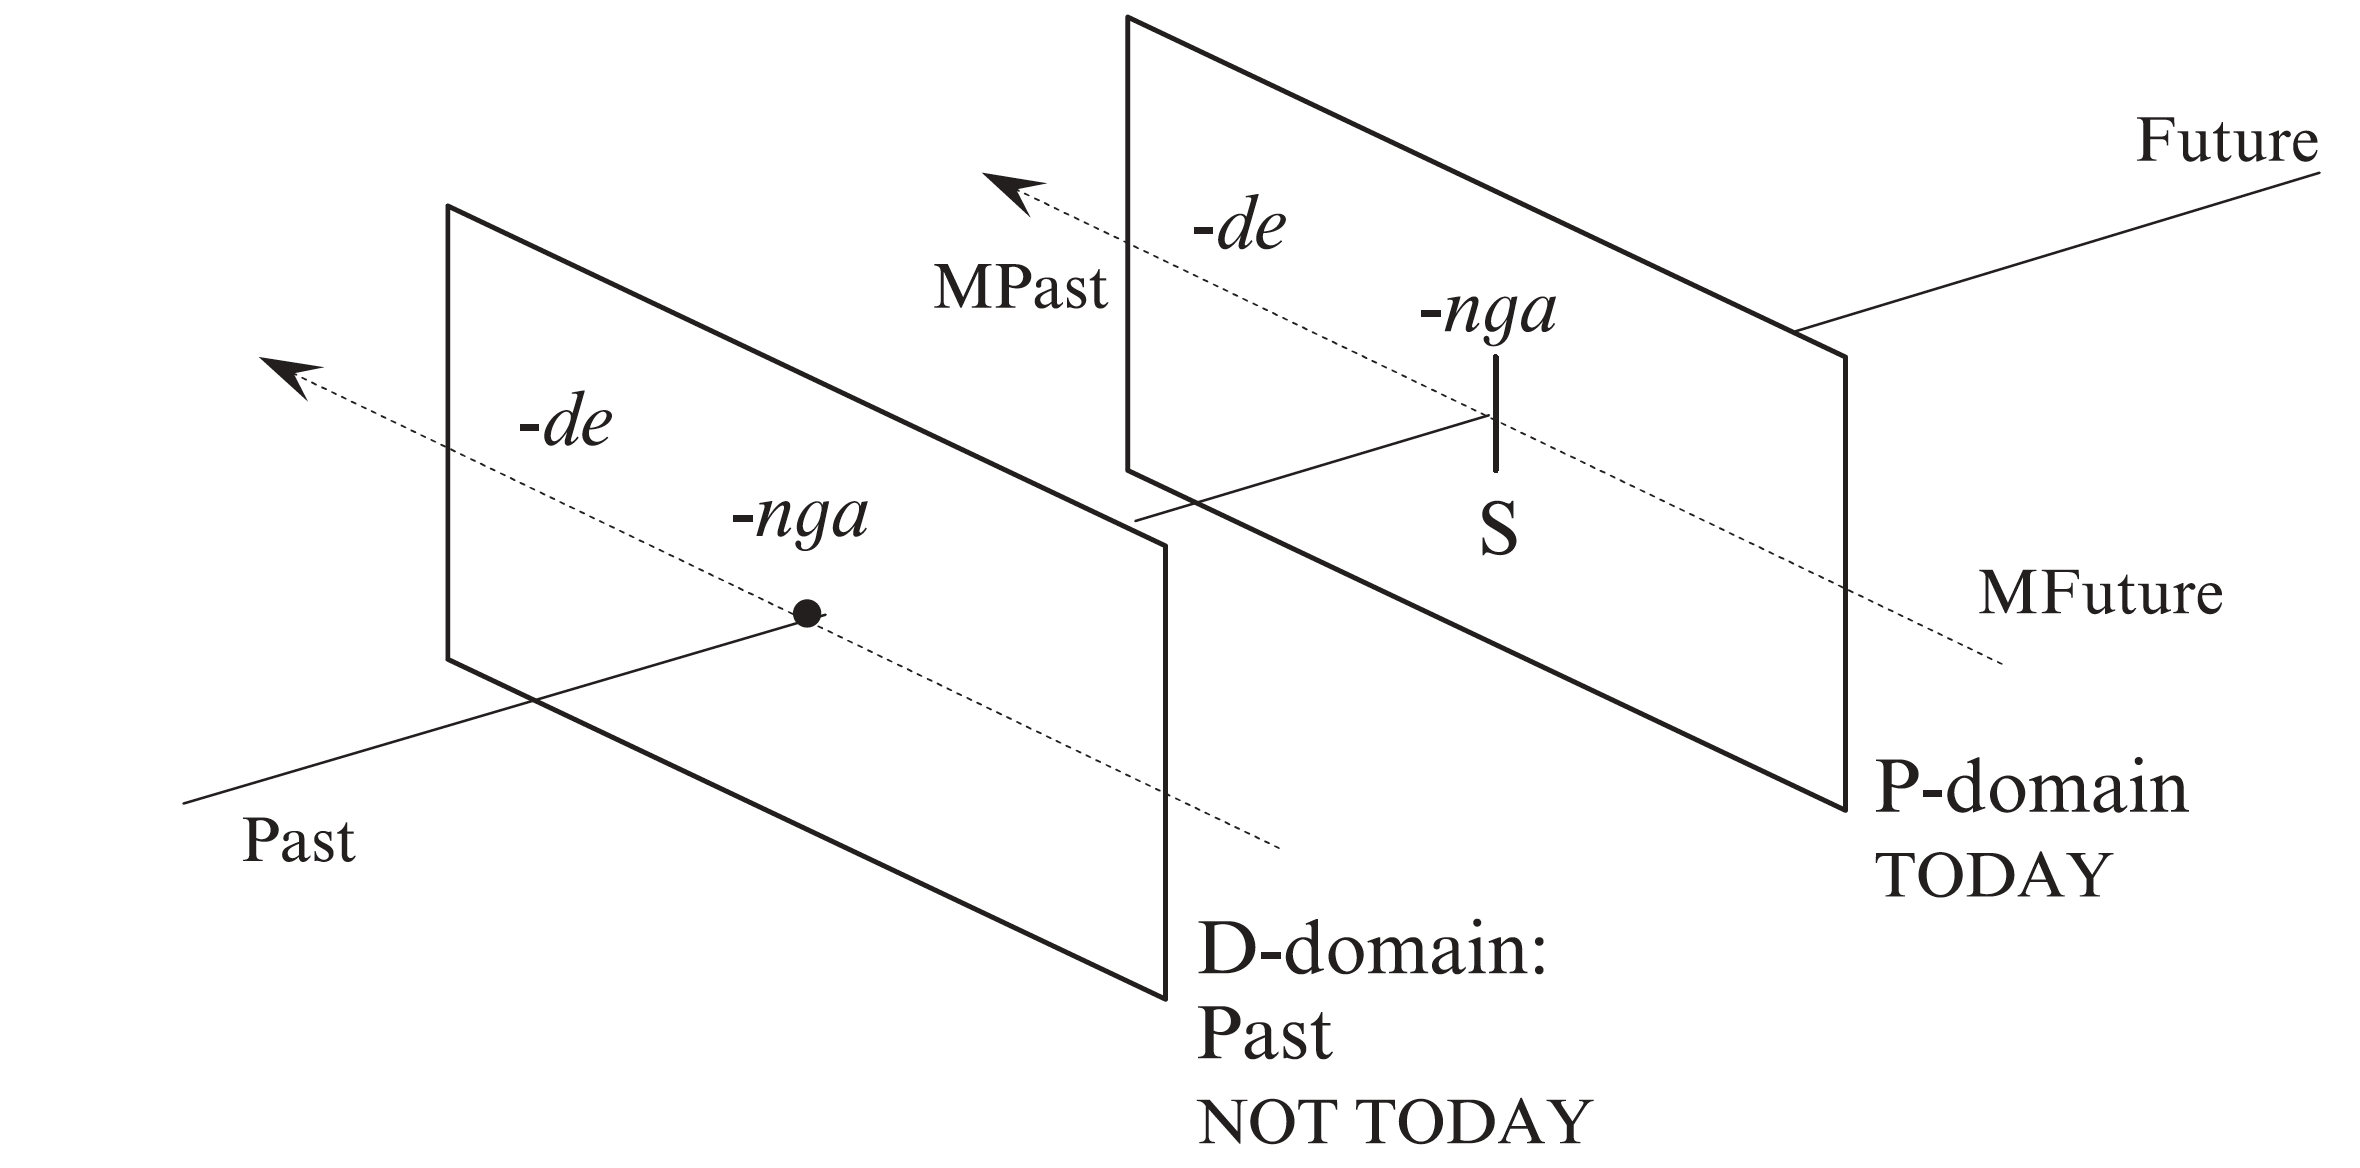
\includegraphics[width=0.9\linewidth]{botnecogdoms}
\end{figure}

\subsection{\textit{Énonciation}, diachrony \& functional unity}

For all the talk of reference frames and cognitive domains, how much closer are we to understanding the motivations for a the encoding of complex temporal remoteness systems of a grammaticalised cyclic tense system?

A number of linguists working on temporal/aspectual distinctions made in Indo\-European languages have drawn \citeauthor{Benveniste1966}'s distinction between ``narrative'' (\textit{récit\slash{}histoire}) and \textit{discours} modes (\textit{plans d'énonciation}).\footnote{Where ``\textit{\textbf{l'énonciation historique} [...] s'agit de la présentation des faits survenus à un certain moment de temps, sans aucune intervention du locuteur dans le récit}'' and \textit{\textbf{discours}} constitutes ``\textit{toute énonciation supposant un locuteur et un auditeur, et chez le premier l'intention d'influencer l'autre en quelque manière}''
	
	(``\textbf{Narrative} comprises the presentation of facts already having occurred at a given moment in time, without any intervention on the part of the speaker'' whereas \textbf{discourse} is understood as ``any utterance that presupposes a speaker and a hearer, where the former intends on influencing their interlocutor in some way.'')\trailingcitation{
	 \citetext{\citealp[238--42]{Benveniste1966}; translation and emphasis mine.}}} To take one example, \citeauthor{Duchet2016}'s \citeyearpar{Duchet2016} study of the usage domains of the Albanian [\gls{sqi}] \textit{\textsc{aorist}} and \textit{\textsc{perfect}},
 \footnote{That is, the synthetic `\textsc{aorist}' (\textit{e kryer e thjeshtë}) and the periphrastic `\textsc{perfect}' \textit{(e kryer)} form `\textsc{have}+past participle' respectively.} suggests the possible utility of this broad \textit{``énonciative''} dichotomy in understanding the distibution of these forms. While past-referring event descriptions in narrative contexts are the \textit{locus classicus} of the \textit{Aorist}, \citeauthor{Duchet2016} show that, in discourse contexts, using this form is also possible in a number of other apparent uses --- including the description of present-holding result states and ``immediate future'' accomplishments. The  \textit{Perfect}, traditionally encoding ``presently relevant result states'' (co-occurring frequently with TFAs that include speech time (`today/this week/this year') and in narratives to encode ``hot news'', also has a range of anterior-type uses: describing states (possibly) occurring prior to (\textsc{aorist-})marked past events.
 
Relatedly, in a survey of remoteness distinctions, \citet[116\textit{ff}]{Dahl1983} identifies a number of languages that appear to treat past differently in ``narrative contexts,'' going on to propose a number of cross-linguistic generalisations that seek to motivate a ``tendency to neutralize distance distinctions in narrative contexts.'' Drawing on a proposed distinction between narrative and discursive contexts, it is conceivable the two reference frames (\textsc{today\slash{}pre-today}) featuring into our analysis of \textsc{wd} temporal reference, in some sense, correspond respectively to \textbf{conversational} and \textbf{narrative} modes. 
 
 That is, in \textbf{conversational} contexts, described events are likely to bear a more immediate relation to the present. Here, a discourse is likely to be concerned with a distinction between {\color{blue}\textsc{past}} and {\color{forest}\textsc{nonpast}}. Conversely, in \textbf{narrative} contexts (accounts of exclusively past events), the distinction between events that held in a {\color{blue}\textsc{remote}}, inaccessible past versus those that held in a relatively \textsc{\color{forest}{recent}} one that more closely resembles the here-and now.\footnote{Compare \citeauthor{Waters1989}'s observation (in his description of Djinaŋ's \textsc{today/remote past}) that ``few stories are set in the time context of the same day as the speech event'' \citeyearpar[188]{Waters1989}.} This usage evokes the phenomenon of the ``narrative/historic present'' --- a commonly attested use cross-linguistically  \citetext{see \citealp{Carruthers2012} for an overview}.\footnote{Cited by \citet[312]{Carruthers2012}, \citeauthor{Facques2007} claims that the historic present ``permet de maintenir l’illusion d’une perspective simultanée du récit, déjà induite par l’emploi du present” (``
 	allows the	illusion to be maintained that the events and the narrative are simultaneous, an illusion already created by use of the present”) \citetext{\citeyear[250--1]{Facques2007}, Carruthers' translation.}} A similar usage of the \textsc{pres} (or \textsc{nonfuture}) is also pointed out by \citet{Stirling2012a}, who shows its extensive use in Kalaw Lagaw Ya [\gls{mwp}], where it functions as a past perfective in narrative contexts.\footnote{This type of usage is apparently widespread in Arnhem Land languages \citetext{\citealt[\textit{e.g.},][]{Bednall2019} for Anindilyakwa [\gls{aoi}]}}
 
On this account, the emergence of \textit{cyclic tense} of the type exhibited in the languages of Maningrida and the westernmost Yolŋu varieties (\textit{viz.} Djinaŋ, Djinba and \gls{wd}) can be explained in terms of a categoricalisation of these two ``reference frames'' that are closely associated with different modes of language use. This corresponds to a hypothetical analysis where: 
\begin{itemize}
	\item Language is used for conversation (pertaining to the eventualities that relate to the here-and-now) and for storytelling (pertaining to events completed prior to the here-and-now)
	\item The function of a \textsc{past}-tense is to signal the settledness and completeness of an event vis-à-vis utterance time. The function of \textsc{present} tenses indicates that the runtime of an event overlaps with utterance time.
	\item The \textsc{past}/\textsc{present} distinction gets reanalysed as \textsc{precontemporary}-{\sc contemporary}: that is \textsc{past/present} relative to a given reference frame (as determined by context (functions) of the utterance.)
\end{itemize}

\subsection{Aspect \& temporal interpreation}
As shown in \S~\ref{sec:djr-prs}, \textsc{wd} verb stems have a strictly dynamic (state change) semantics, a fact that seems to correspond with the recruitment of new strategies for encoding aspectual and modal information (primarily through preverbal auxiliaries and particles.)\footnote{Whereas an explicit aspectual (±\textsc{ipfv}) distinction is actually grammaticalised in the Djinaŋ verbal paradigm, a feature not shared by other Yolŋu languages} The development of this analytic TMA marking system in Dhuwal-Dhuwala is likely to be related to the emergence of a ``cyclic tense'' system where \gls{I} (the erstwhile `\gls{pres}') now obligatorily co-occurs with \textit{ga} `\gls{ipfv}' in order to encode present reference. Compare this fact to the incompatibility between present reference and achievement predicates, where a sentence of the type exemplified in (\nextx) is only available with either a historic present or immediate future reading \citep[an observation following][147]{Vendler1957}.


\pex\textit{Now they find the treasure/win the race/reach the summit}\xe
\pex\a\begingl\gla ŋarra *(ga) \textbf{ḻuka} mänha (dhiyaŋu~bala)\deftagex{wd-contemp}\deftaglabel{prog}//
\glb 1s \gls{ipfv}.\gls{I} drink.\gls{I} water now//
\glft`I'm drinking water (now).'\trailingcitation{[DB~20190405]}//\endgl
\a\begingl\gla ŋarra *(dhu) \textbf{ḻuka} mänha (dhiyaŋu~bala)\deftaglabel{fut}//
\glb 1s \gls{fut} drink.\gls{I} water now//
\glft`I'm going to drink water (now).'\trailingcitation{[DB~20190405]}//\endgl
\a\begingl\gla ŋarra \textbf{ḻuka} mänha (barpuru)//
\glb 1s \gls{ipfv}.\gls{I} drink.\gls{I} water//
\glft`I drank water yesterday.'\trailingcitation{[DB~20190405]}\deftaglabel{pst}//\endgl

\xe

This resembles the situation in \textsc{wd} (\getref{wd-contemp}), where \gls{I} necessarily co-occurs with \textit{ga} `\gls{ipfv}.\gls{I}' or \textit{dhu} `\gls{fut}' to encode present (progressive) or immediate future reference. In the absence of either of these markers, only the \textsc{recent (non-today) past} reading is felicitous.

The relationship between the emergence of cyclic tense in \gls{wd} and evidence for a wholesale restructuring of the language's aspectual system remain a subject for considerable further work and analysis.

\fancybreak

\noindent In view of the semantics for \gls{I} and \gls{III} above, this section has considered possible candidates for functional motivations for the notion of the ``reference frame'' and the ``recycling'' or ``temporal discontinuity'' of tense markers that characterise cyclic tense. On the basis of these considerations, (\nextx) formulates a hypothesis for the emergence of a cyclic tense system of the type described here.

\pex \textbf{\textsc{diachronic hypothesis.}\\Cyclicity as the grammaticalisation of text type}\\
The cyclic tense phenomena exhibited in \textsc{wd} and related languages are a result of the reanalysis of \textsc{present}- and \textsc{past}-tense markers' apparently divergent usage in conversational versus narrative contexts
\xe




 

\section{Conclusion}


This chapter has provided analyses for a number of phenomena related to the temporal interpretation of \textsc{wd} predicates. Of particular importance for developing an analysis of the \textsc{wd} paradigm and \gls{wd}'s tense system is the notion of \textsc{precontemporary instantiation}, a motivation for which was the primary focus of \S~\ref{sec:cyc}.

Drawing on descriptions from \citet{Glasgow1964} and subsequent treatments of the languages of western and central Arnhem Land \citep{Green1987,Green1995,Wilkinson1991,Eather2011,Waters1989}, we proposed a formal treatment of the notion of the ``reference frame'' --- effectively a \textsc{hodiernal/prehodiernal} dichotomy in the \textsc{nonfuture} (``\textsc{realis/actual}'') domain which corresponds to a superinterval of the reference time.

It was argued that the contribution of \gls{III} (the \textsc{precontemporary}) is to constrain reference time to a \textsc{non-final} subinterval of the contextually-supplied reference frame. Via blocking, instantiation of predicates inflected with \gls{I} are felicitous only within the complement of \gls{III}'s range within the realis domain. That is, \gls{I} --- an inflection compatible with present, past and future reference --- is an unmarked form, temporally neutral in its semantics \citetext{compare to treatments of the present, \textit{e.g.}, \citealp{Fleischman1990,Carruthers2012}.\footnote{Also \citeauthor{Dahl1983}'s generalisation that ``[i]t is almost always possible to use the least marked indicative verb form in a narrative past context'' (\citeyear[117]{Dahl1983}, \textit{apud} \citealt{Dahl1980} \textit{n.v}.)}}

 The following chapter extends the account to \gls{II} and \gls{IV} --- the irrealis categories.

%\begin{quote}\small Such meanings probably develop through the interaction of the meaning of the two grams. If a hodiernal past and an anterior (with current relevance) are both developing in the language they would both have a claim to describe situations having just occurred on the same day. If the anterior wins for situations that just occurred but the hodiernal continues to function for situations earlier in the same day, then the result is a discontinuous meaning for the non-hodiernal gram.\trailingcitation{\citep[104]{Bybee1994}}\end{quote}


%\pex
%
%\a \begingl\gla  ŋarra rur'yuna yurruna walu dha-barkthurruna//
%\glft`.'//\endgl
%
%

%
%\xe


\chapter{Modal interpretation \& \textsc{negative asymmetry}\\{\large\sc distinguishing $\boldmath{ \langle \gls{I},\gls{III}\rangle}$ from $\boldmath{ \langle \gls{II},\gls{IV}\rangle}$}}\label{sec:yol-mood}

The basic distributional facts for \gls{II} and \gls{IV} were described in \S~\ref{djr-infl}. As shown there, verb stems receive \gls{II}-marking in future-oriented predications (including imperatives), whereas \gls{IV}-marking is associated most clearly with counterfactual predications and other modal claims with past temporal reference. On the basis of these data, these two inflectional categories appear to be associated with \textit{non-realised} events; and it is this property that distinguishes them from the \gls{I}- and \gls{III}-marked verbs described in the previous chapter (ch.~\ref{sec:djr-temp}).

In this chapter, we interrogate the nature of this apparent ``reality status'' distinction drawn in \gls{wd} (as it is in other Yolŋu Matha varieties) and the expression of mood, modality and modal operators in \gls{wd} more broadly. The distinction between $\langle \gls{I},\gls{III}\rangle$ and $\langle \gls{II},\gls{IV}\rangle$ is ultimately to be understood as one of \textsc{verbal mood}. One phenomenon of particular interest is that of an apparent kinship between negative operators (sentential negators) and modal operators as they are realised in \gls{wd}. It is this kinship that looks to undergird \textit{asymmetric negation} in \textsc{wd} with respect to the marking of reality status; a description of this phenomenon is the goal of \S~\ref{sec:negs}.

\section{Sentential negation and paradigm neutralisation}\label{sec:negs}

As shown in our discussion of the Negative Existential Cycle in Yolŋu Matha (\S~\ref{NEC-yolŋu}, see \textit{p.}~\pageref{sec:nec-djr}), Djambarrpuyŋu has two particles---\textit{yaka} and \textit{bäyŋu}---which both realise standard negation (\textit{i.e.}, that operator whose effect is to reverse the truth value of a given proposition.) The primary distributional distinction between these is that only \textit{yaka} is used to generate negative imperatives (prohibitives) whereas only \textit{bäyŋu} is found in negative existential/quantificational contexts (\getref{bayŋu-negq}--\getref{yaka}). Of interest for current purposes however, is the fact that both of these sentential negators can be shown to directly interact with verbal inflection.


Descriptively, as shown in the data in (\getref{neg-pres}--\getref{neg-pst}), negation appears to trigger a ``switch'' from the `realis-aligned inflections' (\gls{I}~and~\gls{III}) to their `irrealis counterparts' (respectively \gls{II}~and~\gls{IV}). As shown, these latter categories otherwise turn up predominantly in \textit{hypothetical} or \textit{counterfactual} contexts. As we will see, this points to an analysis where the Western Dhuwal(a) inflectional system encodes a \textit{reality status}-based distinction that is neutralised in negated sentences \citep[see also discussion in][356]{Wilkinson1991}. This effect --- which we term a ``negative asymmetry'' \citep[specifically \textsc{\texttt{a/nonreal}}, following][]{Miestamo2005} --- was introduced above (\S~\ref{sec:asymneg}, compare the Gurr-goni \gls{gge} data in \getref{sn-gvg})  and is summarised below in Table \ref{tab:negneut}. Here, we develop a theory of the negative asymmetry as an epiphenomenon of a kinship between \textsc{negative} and (other) \textsc{irrealis} operators.

\begin{table}[h]\centering
	\begin{tabular}{ccc}
		&\multicolumn{2}{c}{\textsc{\textbf{polarity}}} \\
		& \textsc{--neg} & \textsc{+neg}\\\midrule
		&	\gls{I} & \multirow{2}{*}{\gls{II}}\\
		& \gls{II} \\\midrule
		&	\gls{III} & \multirow{2}{*}{\gls{IV}}\\
		& \gls{IV} \\\bottomrule
	\end{tabular}
	\caption{Neutralisation of \gls{I} and \gls{III} inflections under negation.}\label{tab:negneut}
\end{table}


The following examples in (\getref{neg-pres}) show how sentences that receive \gls{I}-marking in positive sentences --- encoding temporal reference to the present or recent past (Ch.~\ref{sec:djr-temp}) --- instead receive \gls{II}-marking under the scope of negation. Each example contains a predication about the present or about the recent past (normally the domain of \gls{I}, as described in the previous chapter.) In thje presence of a negative operator, however, the verb receives \gls{II}-marking. 

(\getref{neg-pres}a-b), for example, presents a near-minimal pair, where the inflection received by a predicate with present reference ``switches'' from \gls{I} to \gls{II} under negation.

\pex\textbf{Exponence of present and recent past reference as \gls{II} under negation}
\deftagex{neg-pres}


\a\begingl%\glpreamble Present-tensed sentence with \gls{I}//
\gla Nhaltja-\textbf{n} \textbf{ga} limurru-ŋgu-ny rom waŋ-\textbf{a}?//
\glb do.how-\gls{I} \gls{ipfv}.\gls{I} 1p.\gls{incl}-\gls{dat}-\gls{prom} law say-\gls{I}//
\glft`What does our law say?'\trailingcitation{\citepalias[~Luk~14.3]{DB}}//\endgl

\a\begingl%\glpreamble Negated present-tense sentence receives \gls{II} marking//
\gla \textbf{yaka} \textbf{gi} \textbf{biyak} rom waŋ-\textbf{i}//
\glb \textbf{\gls{neg}} \gls{ipfv}.\gls{II} do.thusly.\gls{II} law say-\gls{II}//
\glft`That's not how the law is/what the law says.'\trailingcitation{\citep[357]{Wilkinson1991}}//\endgl 




\a\begingl%\glpreamble  Negated present-tense sentence receives \gls{II} marking\\\textsc{context.} Speaker is trying to read from a computer screen.//
\gla \textbf{bäyŋu} ŋarra \textbf{gi} nhä-\textbf{ŋu}//
\glb \textbf{\gls{negq}} 1s \gls{ipfv}.\gls{II} see-\gls{II}//
\glft`I can't see (it).'\\
%\textsc{comment.} \textit{nhäŋu} (`see.\gls{II}') could also mean yesterday in past.
\textsc{\textbf{comment.}} `I didn't see (it) (yesterday)' is also an available reading.\trailingcitation{[AW 2018030]}//\endgl



\a\begingl\gla Ŋarra \textbf{gi} bäyŋu maḻŋ'mara-\textbf{ŋu} waṯu (ŋarraku). + Bili ŋayi \textbf{ga} nhin-\textbf{a} wäŋaŋura//
\glb 1s \textsc{ipfv}.II \gls{neg} appear.\gls{caus}-\gls{II} dog 1s.\gls{dat} \gls{cplv} 3s \gls{ipfv}.\gls{I} sit.\gls{I} house.\gls{loc}//
\glft`I can't find my dog. It lives in the house.'\trailingcitation{[DhG~20190417]}//\endgl



\a\begingl\gla Ŋarra ga djäl-thi-\textbf{rri} giritjirrinyara-wu, + yurru ŋarra bäyŋu-nha \textbf{girritji}//
\glb 1s \gls{ipfv}.\gls{I} want-\gls{vblzr}-\gls{I} dance.\gls{nmlzr}-\gls{dat} but 1s \gls{neg}-\gls{seq} dance-\gls{II}//
\glft`I was wanting to dance (at the \textit{buŋguḻ} yesterday) but I didn't dance (because I'd hurt my leg yesterday.)'\trailingcitation{[DhG~20190417]}//\endgl
%\a\begingl\glpreamble\textsc{context.} A recent hunting trip, narrated in \gls{I} for corresponding positive descriptions.//
%\gla ga \textbf{yaka} ŋayi ŋunhi dharyu-\textbf{rr} \textbf{biyak} djin'tjiŋdhu-\textbf{rr}//
%\glb and \textbf{\gls{neg}} 3s \gls{texd} rain-\gls{II} do.thusly.\gls{II} rain~lightly.\gls{II}//
%\glft`...and it did not rain lightly'\trailingcitation{\citep[357]{Wilkinson1991}}/endgl
\xe


Similarly, in contexts where the temporal reference of the event description predicts that the verb will receive \gls{III}-inflection --- following our description from Ch. \ref{sec:djr-temp}, when referring to the same-day (\textsc{hodiernal}) or the remote past --- when co-occurring with a negative particle (\textit{yaka/bäyŋu}), the verb instead receives \gls{IV}-inflection. This is shown by the data in (\getref{neg-pst}).

 Again, (\getref{neg-pst}a-b) represents a minimal pair where negative marking triggers a ``switch'' from \gls{III} to \gls{IV} inflection. (c) shows the negation of an immediate past event licensing \gls{IV} inflection, (d) shows how a negated, \gls{IV}-inflected predicate can be embedded under a propositional attitude predicate to encode a false belief, and (e) an example of a negated description of the remote past receives \gls{IV} inflection.

\pex \textbf{Exponence of \textsc{today past} and \textsc{remote past} reference as \gls{IV} under negation}\deftagex{neg-pst}
%\a\deftaglabel{munha}\begingl\gla bäyŋu ŋarra gäthur ŋorra-\textbf{nha} manymak-ku-\textbf{nha} munhawu//
%\glb \gls{negq} 1s today lie-\gls{IV} good-\gls{tr}-\gls{IV} nighttime//
%\glft`I didn't sleep well last night'\trailingcitation{\citep[357]{Wilkinson1991}}//\endgl

%\mcom{Though the second clause in (b) also has ŋuli so maybe this is not quite so nice an ex. as originally thought}\a\begingl\gla ŋäthil-nydja ŋarra ga-n dhuwal, ga miltjiri marrtji-n \ bäyŋu ŋarra ŋuli ga-\textbf{nha} nhä-\textbf{nha}//
%\glb earlier-\gls{prom} 1s \gls{ipfv}-\gls{III} \gls{prox} and blind go-\gls{III} \textbackslash \gls{negq} 1s \gls{hab} \gls{ipfv} see-\gls{IV}//
%\glft`I was blind before; I was unable to see'\trailingcitation{\citep[358]{Wilkinson1991}}//\endgl


\a\begingl\gla gathur munhagumirr ŋarra nhä-\textbf{ŋal} warrakan//
\glb today morning 1s see-\gls{III} bird//
\glft`I saw a bird this morning'\trailingcitation{[FW 20180802]}//\endgl


\a\begingl\gla gathur munhagumirr \textbf{bäyŋu} ŋarra nhä-\textbf{nha} warrakan//
\glb today morning \textbf{\gls{negq}} 1s see-\gls{IV} bird//
\glft`I didn't see a bird this morning'\trailingcitation{[FW 20180802]}//\endgl

\a\begingl\glpreamble \textsc{\textbf{context}.} Speaker has dropped a coin.//
\gla Way! \textbf{Bäyŋu} ŋarra nhä-\textbf{nha}?//
\glb Hey! \textbf{\gls{negq}} 1s see-\gls{IV}//
\glft`Ah! Did you see (it)?'\trailingcitation{[AW 20180830]}//\endgl


\a\begingl\glpreamble\textbf{\textsc{context.}} I'm at work explaining to my coworker why my \textit{galay} is angry at me.//
\gla Ŋarraku miyalk maḏakarritj-thi-\textbf{na} bili ŋayi ga \textbf{guyaŋa} ŋarra ga-\textbf{nha} bäyŋu djäma//
\glb 1s.\gls{dat} wife anger-\gls{inch}-\gls{III} \gls{cplv} 3s \gls{ipfv}.\gls{I} think.\gls{I}\footnotemark{} 1s \gls{ipfv}-\gls{IV} \gls{neg} work//
\glft`My wife got angry because she thought I wasn't working today.'\trailingcitation{[DhG~20190417]}//\endgl

\a\begingl\glpreamble \textbf{\textsc{context.}} The speaker grew up in the desert.//
\gla \textbf{bäyŋu} ŋarra ŋuli ga-\textbf{nha} nhä-\textbf{nha} (waltjaṉ) ŋunhi ŋarra yothu yän//
\glb \textbf{\gls{neg}} 1s 	\gls{hab} \gls{ipfv}.\gls{IV} see.\gls{IV} rain \gls{texd} 1s child just//
\glft`When I was young, I hadn't seen [rain]/never saw [rain].'\trailingcitation{[AW~20190501]}//\endgl\xe


%\mcom{It's not clear how I can easily get a the status of this alternation via elicitation (esp. if its intraspeaker..?) or whether I should just abstract away from it. My informants so far seem to have consistently respected this alternation.}
%todo comments about variation across Dhuwal/a
%	Generally, there seems to be a perception (Melanie Wilkinson \textit{pers. comm.}, independently supported by consultant AW [20180830]) that the maintenance of \gls{I} and \gls{III} (the `\textsc{realis}-aligned' inflections) under negation is a characteristic of \textit{Miwatj} varieties of Dhuwal-Dhuwala (\textit{i.e.}, those spoken in towards the East.)
%	
%	\mcom{There's a great comment from my consultant in her translation of a negative sentence. When asked why \textbf{\textit{gi+}II} was used instead of \textbf{\textit{ga+}I} she claims `not happening yet' (20180802-8min)}\citet[356]{Wilkinson1991} notes that ``[she has] not been able to determine a functional basis for this alternation.'' Nevertheless, in his typological survey of standard negation, \citet[558]{Miestamo2005} identifies a cross-linguistically attested mood-based asymmetry where negative marking triggers the appearance of the irrealis or other ``nonrealised''-type modal markings. This phenomenon seems to be particularly well-represented in the languages of the Top End, functional explanations generally emphasising the fact that negated predicates `[belong] to the realm of the non-realized', a domain associated with irrealis marking (\citealt[225]{Miestamo2005}, cf. \citealt[195]{McLellan1992}, \citealp[see also][]{Phillips2019}). These ideas are explored in further detail in Chapter \ref{anY} below.
%	
%	\citet{Wilkinson1991} also suggests that there is insufficient cross-linguistic data to assess a the diachrony (and potential areal diffusion) of this asymmetry (356), although provides a concise review of other authors' observations of Yolŋu varieties (359-60). Data about the interactions between polarity and verbal inflection are provided in the following sections and the question of the development of these asymmetries is treated in Chapter \ref{diaY} below.

The data in (\getref{neg-pres}--\getref{neg-pst}) evince a species of \textsc{negative asymmetry} that is manifested in \gls{wd}. That is, from the four inflections which are availble for encoding temporal and modal information in \gls{wd}, only two (\textit{viz.} \gls{II} and \gls{IV}) are felicitous in sentences that are negated by \textit{yaka} or \textit{bäyŋu}. Figure \ref{NegSchem} schematises the relationship between temporal reference and inflection selection in \textbf{negative clauses} (\textit{cf.} Fig.~\ref{TempSchem}, \textit{p.}~\pageref{TempSchem}.)


\begin{figure}[h]\centering\caption{Apparent interactions between temporal relations and reality status in Djambarrpuyŋu: cyclicty and metricality under negation.}\label{NegSchem}
	\begin{tikzpicture}[scale=1.2]
		% draw horizontal line   
		\draw[<->, line width=.5mm] (0,0) -- (12,0);
		
		%draw rex
		\shade[left color=violet!15!white, right color=orange!15!white] (0,0.02) rectangle (4.8,1.5);
		%	\fill[green!10!white] (2.5,0.02) rectangle (4.8,1.5);
		\fill[violet!10!white] (4.8,0.02) rectangle (6.8,1.5);
		\shade[left color=orange!10!white, right color=green!10!white] (6.8,0.02) rectangle (9.5,1.5);
		\fill[orange!10!white] (9.5,0.02) rectangle (12,1.5);
		
		% draw nodes
		\draw (1.25,0) node[below=3pt] {\textbf{}} node[above=15pt] {\textsc{\gls{IV}}};
		\draw (3.675,0) node[below=3pt] {\textbf{}} node[above=15pt] {\gls{II}};
		\draw (5,0)   node[circle,fill,label=below:$\lfloor{\sl today}$] {} node[below=3pt] {\textbf{}} node[above=3pt] {};
		\draw (7,0) node[diamond,shade,inner color=ochre,outer color=black,label=below:$\boldsymbol{t*}$] {} node[below=3pt] {\textbf{}} node[above=3pt] {\textsc{}};
		\draw (5.8,0) node[below=3pt] {\textbf{}} node[above=15pt] {\textsc{\gls{IV}}};	
		\draw (7.5,0) node[below=3pt] {\textbf{}} node[above=15pt] {\textsc{\gls{II}}};
		\draw (9,0) node[below=3pt] {\textbf{}} node[above=15pt] {\textsc{\gls{I}}};	
		\draw (10.75,0) node[below=3pt] {\textbf{}} node[above=15pt] {\textsc{\gls{II}}};	
		\draw (9.5,0)   node[circle,fill,label=below:${\sl today}\big)$] {} node[below=3pt] {\textbf{}} node[above=3pt] {};
		
		%		%braces
		%		\phantom{	\draw [decorate,decoration={brace,amplitude=4pt},xshift=-0pt,yshift=35pt]
		%			(0.5,0.5) -- (4.5,0.5) node [black,midway,yshift=0.35cm] 
		%			{\footnotesize metricality};
		%
		%			\draw [decorate,decoration={brace,amplitude=4pt},xshift=-0pt,yshift=40pt]
		%			(3.5,0.5) -- (9,0.5) node [black,midway,yshift=0.35cm] 
		%			{\footnotesize cyclicity};}
		
	\end{tikzpicture}
\end{figure}

Further complicating things, while \gls{III} is categorically ruled out in negative sentences, \gls{I} ``survives'' when (and \underline{only when}) the predicate refers to the \textsc{same-day future.} That is, the \gls{I}/\gls{II} distinction is \textit{not} neutralised in negative sentences with reference to events happening later on the day of utterance (whereas the distinction \textit{is} neutralised in all \textsc{nonfuture} contexts.) Examples are provided in (\getref{futneg}-\getref{prsneg}).


\pex \textbf{Future marking is unaffected by polarity/the presence or absence of sentential negation}	\deftagex{futneg}
\a\begingl\glpreamble \gls{I} with \textsc{same-day future} reference ``survives'' negation//
\gla ŋarra (yaka) ŋunha \textbf{dhu} ḻuk-\textbf{a} dhiyaŋ~bala//
\glb 1s (\gls{neg}) \gls{fut} \gls{dist} eat-\gls{I} now//
\glft`I will (not) eat them [\textit{ḻatjin}] right now.'\trailingcitation{[AW~20190422]}//\endgl

\a\begingl\glpreamble \textsc{post-hodiernal} referring predicates receive \gls{II}-inflection//
\gla (bäyŋu) ŋarra \textbf{dhu} buḻ'yu-\textbf{rr} barpuru//
\glb \gls{neg} 1s \gls{fut} play-\gls{II} tomorrow//
\glft`I will (not) play [football] tomorrow.'\trailingcitation{[AW~20190429]}//\endgl
\xe

\pex \textbf{A minimal pair: \gls{I} changes to \gls{II} in present-referring negative sentences}\deftagex{prsneg}
\a\begingl\glpreamble Negative present predication with \gls{II}//
\gla (dhiyaŋ~bala) \textbf{bäyŋu} ŋarra \textbf{gi} nhä-\textbf{ŋu} mukulnha//
\glb now \textbf{\gls{neg}} 1s \gls{ipfv}.\gls{II} see-\gls{II} aunt.\gls{acc}//
\glft`I don't/can't see my aunt (right now).'\trailingcitation{[AW~20190501]}//\endgl
\a\begingl\glpreamble Positive present predication with \gls{I}//
\gla (dhiyaŋ~bala)  ŋarra \textbf{ga} nhä-\textbf{ma} mukulnha//
\glb now 1s \gls{ipfv}.\gls{I} see-\gls{I} aunt.\gls{acc}//
\glft`I'm watching my aunt (right now).'//
\endgl\xe


\section{The meaning of the modal particles}
\label{sec:modals}
%todo label `anY' has been de-defined
%\section{The realm of the nonrealized}\label{anY}
In \S~\ref{djr-infl}, we saw that predicates which receive \gls{II}- and \gls{IV}-inflection co-occur with some operator that encodes some flavour of irrealis-associated meaning --- suggesting what \citet[145]{Palmer2001} labels a ``joint marking system'' (\textit{i.e.}, that reality is multiply indicated, in this case by suffixation in addition to a preverbal particle.) 

For \gls{II}, these are predominantly represented by \textit{dhu} `\gls{fut}' and \textit{balaŋ(u)} `\gls{irr}' in addition to clauses with imperative syntax. \gls{IV} tends to co-occur with \textit{balaŋ} `\gls{irr}' in addition to \textit{ŋuli} `\gls{hab}'.\footnote{I adopt the (metalinguistic) labels \gls{fut} for \textit{dhu} \citep[following][]{Wilkinson1991} and \gls{mod} for \textit{balaŋ(u)}. As we will see, these descriptions aren't necessarily completely semantically adequate, but will be sufficient for current purposes. \citet{Wilkinson1991} glosses \textit{ŋuli} as `\gls{hab}' or `\gls{hyp}' depending on its apparent function in the clause (as a marker of \textsc{habituality} or of a conditional antecedent (``\textsc{hypotheticality}'').)\label{irr-glossing}} Importantly, and as we will see, these expressions all appear to lexicalise strictly \textbf{root} (circumstantial\slash{}non-epistemic) modalities \citep[\textit{contra claims in}][123]{VanderWal1992}.

This section seeks to model the irrealis domain using the ``branching time framework'' introduced in \S~\ref{LitRev} in order to propose a semantics for \gls{wd} modal particles. This will permit for forming a set of generalisations over the distribution of \gls{II} and \gls{IV}.



	%\subsection{The branching time framework}\label{sec:wd-BT-fwk}
	%
	%Authors working in intensional semantics have, in recent work, deployed a ``branching time'' framework in order to model relationships between temporal and modal reference (an overview provided in Chapter \ref{IntroCh} and implemented in the semantic treatment of \textit{bambai} in Chapter \ref{bambai.semx}). Here, I spell out a number of basic assumptions that will ultimately assist in formalising temporal and modal expressions in WD. One of the primary payoffs of the branching time is the formalisation of Prior's observations about the asymmetries of the past and the future \citep[see also][]{Copeland2020,Dowty1977,Thomason1970,Thomason1984}. The version I adopt here follows closely from recent work on the realis-irrealis distinction \citep{VonPrince2019,Krifka2016} and other insights about temporal and modal interaction (\citealp[e.g.][]{Condoravdi2002,Ippolito2013}, a.o.)
	%
	%
	%A branching-time frame $ \mathfrak U=\langle \mathcal I,\prec\rangle $ assumes a partially ordered set of indices $ \mathcal I $ --- in effect world-time pairs $ \langle w,t\rangle  $. A branch (similar to ``history'' for other authors \citep{Thomason1970,Dowty1977}) $ b\ni i $ through any $ i\in\mathcal I $ is a linearly ordered subset of $ \mathcal I $ --- that is, where $ i=\langle w,t\rangle $,\\ $ b\ni i=\{\big\langle\langle w,t\rangle,\langle w,t'\rangle,\langle w,t''\rangle,\hdots,\langle w,t_n\rangle\big\rangle\}$. A branch, then, effectively models the possible development of a given world through time.\footnote{Note that these frameworks normally take indices to represent world-time pairs. I assume that this model can be extended relatively straightforwardly to capture interval semantic notions (\citealp[e.g.][]{Landman1991,Dowty1982,Bennett} a.o.).}
	%\begin{figure}[h]
	%	\caption{A branching times frame following von Prince \citeyearpar[e.g.,][591]{VonPrince2019}. Vertically aligned indices are taken to index the same time.}\centering
	%	\begin{tikzpicture}
	%		[scale=1.5,level distance=9mm,
	%		every node/.style={fill=black,circle,inner sep=1.5pt},
	%		level 1/.style={sibling distance=10mm},
	%		level 2/.style={sibling distance=8mm},
	%		level 3/.style={sibling distance=4mm},
	%		level 4/.style={sibling distance=2mm},
	%		edge from parent/.style={draw}]
	%		\node {} [grow=right]
	%		child {node {} edge from parent[densely dotted]
	%			child {node {}
	%				child {node {}
	%					child {node {}}
	%					child {node {}}}
	%				child {node {}
	%					child {node {}}
	%					child {node {}}}}
	%			child {node {}
	%				child {node {}
	%					child {node {}}
	%					child {node {}}}
	%				child {node {}
	%					child {node {}}
	%					child {node {}}}}}
	%		child[missing]
	%		child {node {}
	%			child {node {} edge from parent[densely dotted]
	%				child {node {}
	%					child {node {}}
	%					child {node {}}}
	%				child {node {}
	%					child {node {}}
	%					child {node {}}}}
	%			child {node {} edge from parent[densely dotted]
	%				child {node {}
	%					child {node {}}
	%					child {node {}}}
	%				child {node {}
	%					child {node {}}
	%					child {node {}}}}
	%			child {node [style={fill=red},label=above:$ \boldsymbol{i*} $] {}
	%				child {node {} edge from parent[densely dashed]
	%					child {node {}}
	%					child {node {}}}
	%				child {node {} edge from parent[densely dashed]
	%					child {node {}}
	%					child {node {}}}}};
	%\end{tikzpicture}\end{figure}
	%
	%
	%
	%
	%
	%
	%
	%\Citet{VonPrince2017a,VonPrince2019} establishes a formal trichotomy between the \textsc{actual, potential} and \textsc{counterfactual} domains by appealing to this framework. This is reproduced in (\nextx).
	%
	%\pex Given a contextually defined \textsc{actual present} $( i*=\langle w*,t*\rangle )$, $ \mathcal I $ can be partitioned into three subdomains:
	%\a The \textsc{actual} (past/present) = $ \{i\mid i\preceq i*\} $\\
	%Compare this notion to the equivalent one of \textit{metaphysical alternatives to $ w $ at $ t $} introduced in Ch. \ref{bambai}: $ \{w'\mid w\approx_t w\} $.
	%\a The \textsc{potential} (future) = $ \{i\mid i\succ i*\} $
	%\a The \textsc{counterfactual} = $ \{i\mid i \text{ is unordered w/r/t } i* \} $\deftagex{trichot}\deftagpage{vP-bt}
	%\xe





\subsection{\textit{dhu}: irreality and the \textsc{future}}

Shown above (predominantly in \S~\ref{desc-ii}),  \textit{dhu} `\gls{fut}' occurs in sentences with future temporal reference -- with either \gls{I} or \gls{II} marking, depending on whether the reference time of the proposition is the same as the day of speech or beyond. This is shown again by the data in \getref{dhu-fut}.

Relatedly, the data in (\getref{dhu-nec}) show that \textit{dhu} appears to also be compatible with other circumstantial modalities; for example, with (\getref{dhu-nec.d}) deontic, (\getref{dhu-nec.b}) bouletic and (\getref{dhu-nec.t}) teleological readings. In all these contexts, we can model \textit{dhu} as universally quantifying over a (subset of) a circumstantial modal base.

\pex \textbf{\textit{dhu} `\gls{fut}' encoding future tense with \gls{I}- and \gls{II}-inflections}
\a\begingl\gla barpuru goḏarr ŋarra \textbf{dhu} nhä-\textbf{ŋu}//
\glb funeral tomorrow 1s \gls{fut} see-\gls{II}//
\glft`I'll watch the funeral tomorrow.'\trailingcitation{}\deftagex{dhu-fut}//
\endgl
\a\begingl\gla mukul \textbf{dhu} \textbf{gi} nhin-\textbf{i} raŋi-ŋur goḏarr//
\glb aunt \textbf{\gls{fut}} \gls{ipfv}.\gls{II} sit-\gls{II} beach-\gls{loc} tomorrow//
\glft`Aunty will be sitting on the beach tomorrow.'\trailingcitation{[AW~20190409]}//\endgl
\a\begingl\gla limurru \textbf{dhu} ḻuk-\textbf{a} maypal yalala milmitjpa//
\glb 1d.\textsc{excl} \textsc{fut} consume-\gls{I} shellfish later evening//
\glft `We're having shellfish this evening.'\trailingcitation{[DhG~20190417]}//
\endgl
\xe
\pex \textbf{\textit{dhu} `\gls{fut}' and other flavours of modal necessity}\deftagex{dhu-nec}
\a\begingl\gla Way! Nhe \textbf{dhu} gurruk-\textbf{ama} djoŋgu'!//
\glb Hey! 2s \gls{fut} carry-\gls{I} hat//
\glft`Hey! You must wear a helmet!'\trailingcitation{[DhG~20190405]}\deftaglabel{d}//\endgl
\a\begingl\gla djamarrkuḻi \textbf{dhu} yaka wurraŋatjarra'\textbf{y-irr}\deftaglabel{b}//
\glb children \gls{fut} \gls{neg} cruel.\gls{inch}-\gls{I}//
\glft`The children mustn't be disobedient.'\trailingcitation{[AW~20190429]}//\endgl
\a\begingl\gla ŋarra \textbf{dhu} plane-dhu marrtji, bili mutika-miriw\deftaglabel{t}//
\glb 1s \gls{fut} plane-\gls{erg} go-\gls{I}|\gls{II} \gls{cplv} car-\gls{priv}//
\glft`I'll have to go by plane because I don't have a car.'\trailingcitation{[AW~20190429]}//\endgl
\xe

\noindent Suggested in \S~\ref{desc-ii}, \textit{dhu} appears exclusively in \textit{future-oriented} predications, apparently \textit{with present perspective} (that is, in predications about the future as calculated at speechtime, \citealp[see][]{Condoravdi2002}.) The relation between temporal reference and inflection in \textit{dhu-}marked sentences is schematised in figure \ref{FutSchem}.

\begin{figure}[h]\centering\caption{(In)compatibility of modal particle \textit{dhu} `\gls{fut}' with temporal reference \& inflectional category.}\label{FutSchem}
	\begin{tikzpicture}[scale=.9]
		% draw horizontal line   
		\draw[<->, line width=.5mm] (0,0) -- (12,0);
		
		%draw rex
		\fill[gray!10!white] (0,0.02) rectangle (4.8,1.5);
		%	\fill[green!10!white] (2.5,0.02) rectangle (4.8,1.5);
		\fill[gray!10!white] (4.8,0.02) rectangle (6.8,1.5);
		\fill[green!10!white] (6.8,0.02) rectangle (9.5,1.5);
		\fill[orange!10!white] (9.5,0.02) rectangle (12,1.5);
		
		% draw nodes
		\draw (1.25,0) node[below=3pt] {\textbf{}} node[above=10pt] {\textsc{\textbf{*}}};
		\draw (3.675,0) node[below=3pt] {\textbf{}} node[above=10pt] {\textbf{*}};
		\draw (5,0)   node[circle,fill,label=below:$\lfloor{\sl today}$] {} node[below=3pt] {\textbf{}} node[above=3pt] {};
		\draw (7,0) node[diamond,shade,inner color=ochre,outer color=black,label=below:$\boldsymbol{t*}$] {} node[below=3pt] {\textbf{}} node[above=3pt] {\textsc{}};
		\draw (5.8,0) node[below=3pt] {\textbf{}} node[above=10pt] {\textsc{\textbf{*}}};	
%		\draw (7.5,0) node[below=3pt] {\textbf{}} node[above=10pt] {\textsc{\gls{II}}};
		\draw (8.25,0) node[below=3pt] {\textbf{}} node[above=10pt] {\textsc{\gls{I}}};	
		\draw (10.75,0) node[below=3pt] {\textbf{}} node[above=10pt] {\textsc{\gls{II}}};	
		\draw (9.5,0)   node[circle,fill,label=below:${\sl today}\big)$] {} node[below=3pt] {\textbf{}} node[above=3pt] {};
		
		%		%braces
		%		\phantom{	\draw [decorate,decoration={brace,amplitude=4pt},xshift=-0pt,yshift=35pt]
		%			(0.5,0.5) -- (4.5,0.5) node [black,midway,yshift=0.35cm] 
		%			{\footnotesize metricality};
		%
		%			\draw [decorate,decoration={brace,amplitude=4pt},xshift=-0pt,yshift=40pt]
		%			(3.5,0.5) -- (9,0.5) node [black,midway,yshift=0.35cm] 
		%			{\footnotesize cyclicity};}
		
	\end{tikzpicture}
\end{figure}


\noindent On the basis of this range of usage, we have reason to treat \textit{dhu} as a modal expression. Here we adopt the quantificational (pragmatic domain restriction) approach to modal semantics introduced in \S~\ref{sec:kratzer} and adapt an analysis in the style of \citeauthor{Condoravdi2003}'s (\citeyear{Condoravdi2002,Condoravdi2003} a.o.) unified treatment of \textit{will} on its `future auxiliary' and modal uses .


The different ``flavours'' of \textit{dhu} can be modelled using a standard ordering semantics (introduced above, \textit{p.}~\pageref{ex:randi}.) The contextual parameter \textit{c} makes available a number of conversational backgrounds against which \textit{dhu} is interpreted --- namely a circumstantial modal base $ \underset{\textsc{circ}}{m} $ and some type of ordering source $ o $. 

The function \textsc{best} selects the ``best'' worlds in a circumstantial modal base, according to how well they conform with whatever set of propositions is returned by $ o $. Depending on which ordering source is provided by context, these conversational backgrounds can be thought of as sets of:
\begin{itemize}
	\item speaker expectations (\textsc{stereotypical} ordering sources, in the case of \textsc{future}/prediction uses), 
	\item relevant rules \& regulations (in the case of \textit{deontic} uses),
	\item  relevant desires (in the case of \textit{bouletic} uses),
	\item  relevant goals/ends (in the case of \textit{teleological} uses) \trailingcitation{\textit{etc.}}
\end{itemize}	
	
\noindent Ultimately, then, \textit{dhu} is ``pragmatically ambiguous'' between (at least) the types of readings described here and depends for its interpretation on the successful retrieval of an ordering source. This is a desirable consequence given, for example, the availability of a future/prediction reading of (\getfullref{dhu-nec.t}) as well as the teleological reading provided in the translation above.
	
	
Despite the range of modal flavours available to \textit{dhu}, it does exhibit an apparent incompatibility between \textsc{wd} modal particles and \textbf{epistemic} conversational backgrounds. Consequently we claim that \textit{dhu} is lexically specified for non-epistemic modal bases (compare \citet{Kratzer1981}; this is modelled by assuming that \textit{dhu} presupposes that context $ c $ makes available an appropriate ordering source in addition to some relevant set of circumstances \citealp[see also][]{Peterson2010,Rullmann2008,Matthewson2016} a.o.)



\pex \textbf{Lexical entry for \textit{dhu} `\gls{fut}'}

\deftagex{dhu-sems}\textit{dhu} is only defined if context makes available a circumstantial modal base~$ m $

$ \denote[c]{\textit{dhu}}=\lambda P\lambda i:\forall b\big[b\in\underset{o}{\textsc{best}}\big(\underset{\textsc{circ}}{\cap m(i)}\big)\to\exists^b i'[i'\succeq i\wedge P(i')]\big] $

%.\forall w'\big[w'\in\underset{o}{\textsc{best}}\big(\cap\textsc{circ}(w),t\big)\to \textsc{Inst}\big(P,w',[t,\infty)\big)\big]$\\
\textit{dhu $ P $} %, uttered in some reference index $ i $,
 asserts that -- in the best branches of the modal base (according to some ordering source $ o $) -- there will be some  index $ i' $ --- a successor to $ i $ --- at which the property $ P $ holds.%\footnote{The relation ``\textsc{Inst}antiation'' (also given as \textsc{at}) is taken to hold between a property of events, a time, and a world when there is some event of a given type that is contained within that time: $$ \textsc{Inst}(P,w,t)=\exists e[P(e)\wedge\tau(e,w)\sqsubseteq t] $$ See also \citet{Condoravdi2003,Condoravdi2014} a.o.}
 %\marginnote{it seems that M16,R+M18 treat the circ. mb as a presupposition: i.e. relevant modals are defined iff $ f $ is circ.}
\xe%todo\marginnote{potentially want to say that \textsc{inst} holds at $ t* $}[-1in]

\subsection{\textit{balaŋ(u)} \& modal claims}

In addition to \textit{dhu}, \gls{wd} deploys a number of other modal particles: \textit{balaŋ/balaŋu} `\gls{mod}' the most frequently occurring among them. \textit{balaŋ(u)} occurs with verbal predicates categorically inflected for either \gls{II} (shown in \getref{balaŋ-ii}) or \gls{IV} (shown in \getref{balaŋ-iv}).

The distinction in interpretation between these two sets of data is the \textit{temporal interpretation} of the modal. In all cases, \textit{balaŋ(u)}, appears to receive a root possibility reading. Similarly to \textit{dhu}, then, we model \textit{balaŋ(u)} as a quantifier over a (subset of a) circumstantial modal base. Whereas \gls{II}-marking induces a future possibility reading, co-occurrence with \gls{IV}-marking tends to encode varieties of past possibility (including counterfactual) readings.

A number of examples of predications about possible (future) events are shown in (\nextx). These examples show that a range of predictive/modal ``strengths'' are available to \textit{balaŋ}-sentences (the speaker's apparent confidence in the instantiation of the predicate.) Modal particles can also co-occur (``stack''): in (\getfullref{balaŋ-ii.smoke}--\getref{balaŋ-ii.cat}), in both cases, the presence of multiple modals appears to decrease the force of the claim.\footnote{The meaning of \textit{bäynha} (glossed here also as \gls{mod}) is unclear. \citet[670]{Wilkinson1991} analyses this item as \textit{bäy-nha} `until-\gls{seq}', although my consultant treats it as virtually synonymous with \textit{balaŋu}.
%\exdisplay\begingl\gla yolŋu dhu nhina wäŋaŋur nhanukiyingal ga yaka marrtji ganarrtham ŋayi \textbf{dhu} \textbf{balaŋ} \textbf{bäynha} mirith-\textbf{irr} ga rirrikthun ga marrtji watjpillil//
%\glb person \gls{fut} sit.\gls{I} home.\gls{loc} 3s.\gls{obl} and \gls{neg} go.\gls{I} leave.\gls{I} 3s \gls{fut} \gls{mod} \gls{mod} \gls{intens}
%\glft`[Another parole condition might be that] the offender must stay in his home community and not leave unless for a medical emergency.'//\endgl\xe
}

%\marginnote{\textit{balaŋ} may be better glossed as just \gls{mod}, where \gls{irr} is reserved to describe verbal mood.}
\pex \textbf{\textit{balaŋ(u)} `\gls{mod}' and \gls{II}-inflection}\deftagex{balaŋ-ii}

\a\begingl\gla ŋarra \textbf{balaŋu} ḻuk-\textbf{i}/(*-a) gapu, ŋanydja monuk ŋayi gapu\deftaglabel{drink}//
\glb 1s \textbf{\gls{mod}} consume-\gls{II}/*\gls{I} water but saline 3s water//
\glft`I would drink some water but this water's salty.'\trailingcitation{[DhG~20190405]}//\endgl
\a\begingl\gla ŋarra ŋuli ga bitjan bili warguyun ŋunhi \textup{recorder} \textbf{balaŋu} bakthu-\textbf{rru}\deftaglabel{break}//
\glb 1s \gls{hab} \gls{ipfv}.\gls{I} thus.\gls{I} \gls{cplv} worry.\gls{I} \gls{texd} recorder \textbf{\gls{mod}} break-\gls{II}// 
\glft`I'm always worried that the recorder will/could break.'\trailingcitation{[DhG~20190417]}//\endgl

\a\begingl\gla ŋarra \textbf{balaŋu} (bäynha) dhiŋg-\textbf{uŋu} ŋawalul'yu\deftaglabel{smoke}//
\glb 1s \textbf{\gls{mod}} (\gls{mod}) die-\gls{II} smoke.\gls{erg}//
\glft`I could die from the smoke.'\trailingcitation{[DhG~20190405]}//\endgl

\a\begingl\gla ŋayi \textbf{balaŋ} \textbf{dhu} djaṉŋar-\textbf{thi}\deftaglabel{cat}//
\glb 3s \gls{mod} \gls{fut} hunger-\gls{inch}.\gls{II}//
\glft`It (the cat) might get hungry.'\trailingcitation{[AW~20190429]}//\endgl



\xe

Predications about ``past possibilities'' are indicated by the co-occurrence of \textit{balaŋ(u)} and \gls{IV} as seen in (\nextx). A counterfactual reading is available to each of the three sentences. In conditionals (i.e., those counterfactual predications with an explicit antecedent) both clauses are inflected with \gls{IV} -- an example is given in (\getfullref{cond.iv}).


\pex \textbf{\textit{balaŋ(u)} `\gls{irr}' and \gls{IV}-inflection}\deftagex{balaŋ-iv}

\a\begingl\gla nhe \textbf{balaŋu} malkthu-\textbf{nha}//
\glb 2s \textbf{\gls{mod}} accompany-\gls{IV}//
\glft `You should/would have gone with (him).'\trailingcitation{[DhG~20190413]}//\endgl


\a\begingl\gla ŋarra gana guyaŋa-na waṯuy \textbf{balaŋu} ḻuka-\textbf{nha} chocolate//
\glb 1s \gls{ipfv}.\gls{III} think-\gls{III} dog.\gls{erg} \textbf{\gls{mod}} eat-\gls{IV} chocolate//
\glft`I'd thought the dog might/would eat the chocolate.'\trailingcitation{[DhG~20190413]}//\endgl

\a\begingl\gla ŋarra-nha \textbf{balaŋu} ḻuku walala mitthu-\textbf{na}... yurru ŋarra manymak-thirri//
\glb 1s-\gls{acc} \textbf{\gls{irr}} foot 3p cut-\gls{IV} but 1s good-\gls{inch}.\gls{I}//
\glft`They would have amputated my foot, but I got better.'\trailingcitation{[DhG~20190417]}\deftaglabel{ḻuku}//\endgl
\xe
%\marginnote{I actually don't currently have any way of specifying that \textit{dhu} is necessarily assumes pres-persp \& future-orientn unlike \textit{balaŋ}.}

In explicit conditional statements, both antecedent and consequent are marked with a modal particle. \textit{Ŋuli} (glossed here as \gls{hyp}, see {\sf fn} \ref{irr-glossing}) normally seems to mark antecedent clauses, although as shown in \getref{cond.sick}, the co-ordination of two \textit{balaŋ(u)}-clauses also seems to give rise conditional interpretation (compare the discussion of \textit{modal subordination} phenomena in Part \ref{bambai} (\S~\ref{bambai.subord}.))


\pex\deftagex{cond} \textbf{Conditional constructions licensing \gls{II} and \gls{IV} inflection (in indicative and counterfactual contexts respectively)} 


\a\begingl\gla ŋarra \textbf{dhu} wargu-\textbf{yurr}, \textbf{ŋuli} ŋarra \textbf{dhu} bäyŋu gurrup-\textbf{ulu} ŋatha butjigitnha. ŋayi \textbf{dhu}/\textbf{balaŋ} djaṉŋar-\textbf{thi}.//
\glb 1s \textbf{\gls{fut}} worry-\gls{vblzr}.\gls{II} \gls{hyp} 1s \textbf{\gls{fut}} \gls{neg} give-\gls{II} food cat.\gls{acc} 3s \textbf{\gls{fut}/\gls{mod}} hunger-\gls{inch}.\gls{II}//
\glft`I'd be worried if I didn't feed the cat. It would/could get hungry (if I didn't.)'\trailingcitation{[AW~20190429]}\deftaglabel{ii}//\endgl

\a\begingl\gla ŋarra \textbf{balaŋu} ḻuk-\textbf{i}, ŋarra \textbf{balaŋu} rirrikth-\textbf{urru}//
\glb 1s \textbf{\gls{mod}} eat-\gls{II} 1s \textbf{\gls{mod}} get.sick-\gls{II}//
\glft`If I eat (it), I might be sick.'\trailingcitation{\citep[\textsc{l}96]{Lowe1996}}\deftaglabel{sick}//\endgl

\a\begingl\glpreamble \textsc{context.} Despite Mum's imprecations to feed the cat, I maintained a poor feeding ethic. The cat is now emaciated and Mum suggests:\deftaglabel{iv}//
\gla \textbf{Ŋuli} \textbf{balaŋu} nhe ŋatha gurrupa-\textbf{nha} butjigit-nha, ŋayi \textbf{balaŋu} ŋutha-\textbf{nha}//
\glb \gls{hyp} \gls{mod} 2s food give-\gls{IV} cat-\gls{acc} 3s \gls{mod} grow-\gls{IV}//
\glft`Had you fed the cat, it would have grown.'\trailingcitation{[DhG~20190405]}//\endgl

\xe


Unlike \textit{dhu} `\gls{fut}', then, \textit{balaŋ} sentences appear to compatible with past temporal reference, which is always indicated by \gls{IV} marking. That is, temporal remoteness distinctions of the type described in chapter \ref{sec:djr-temp} --- which, as shown in \S~\ref{sec:negs} were preserved in negative clauses --- are neutralised in these modal contexts. A clear example is given in (\nextx), where a predicate describing same non-realised event (going out \textsf{yesterday} to collect \textit{maypal}) receives \gls{II} inflection when occurring with a negative marker (\textit{bäyŋu}) but \gls{IV} when occurring with a modal particle (\textit{balaŋ}). Figure \ref{BalSchem} gives another schematic representation of the relations between temporal reference and inflectional suffix, this time in contexts with the root possibility modal \textit{balaŋ(u)}.



\pex
\begingl\gla barpuru ŋarra guyaŋ-\textbf{a} balaŋ limurr bu-\textbf{nha} maypal… + yurru bäyŋu napurru bu-\textbf{ŋu} maypal//
\glb yesterday 1s think-\gls{I} \gls{mod} 1p.\gls{incl} hit-\gls{IV} shellfish but \gls{neg} 1p.\gls{excl} hit-\gls{II} shellfish//
\glft`Yesterday, I \textcolor{forest}{thought} we would \textcolor{violet}{collect} shellfish, but we didn't \textcolor{ochre}{collect} shellfish.'\trailingcitation{[AW~20190429]}//\endgl\xe


\begin{figure}[h]\centering\caption{Compatibility of modal particle \textit{balaŋ} `\gls{mod}' with temporal reference \& inflectional category.}\label{BalSchem}
	\begin{tikzpicture}[scale=1]
		% draw horizontal line   
		\draw[<->, line width=.5mm] (0,0) -- (12,0);
		
		%draw rex
		\fill[violet!10!white] (0,0.02) rectangle (6.8,1.5);
		%	\fill[green!10!white] (2.5,0.02) rectangle (4.8,1.5);
%		\fill[gray!10!white] (4.8,0.02) rectangle (6.8,1.5);
%		\fill[green!10!white] (6.8,0.02) rectangle (9.5,1.5);
		\fill[orange!10!white] (6.8,0.02) rectangle (12,1.5);
		
		% draw nodes
%		\draw (1.25,0) node[below=3pt] {\textbf{}} node[above=10pt] {\textsc{\textbf{*}}};
		\draw (3.675,0) node[below=3pt] {\textbf{}} node[above=15pt] {\gls{IV}};
		\draw (5,0)   node[circle,fill,label=below:$\lfloor{\sl today}$] {} node[below=3pt] {\textbf{}} node[above=3pt] {};
		\draw (7,0) node[diamond,shade,inner color=ochre,outer color=black,label=below:$\boldsymbol{t*}$] {} node[below=3pt] {\textbf{}} node[above=3pt] {\textsc{}};
%		\draw (5.8,0) node[below=3pt] {\textbf{}} node[above=10pt] {\textsc{\textbf{*}}};	
		%		\draw (7.5,0) node[below=3pt] {\textbf{}} node[above=10pt] {\textsc{\gls{II}}};
%		\draw (8.25,0) node[below=3pt] {\textbf{}} node[above=10pt] {\textsc{\gls{I}}};	
		\draw (9.5,0) node[below=3pt] {\textbf{}} node[above=15pt] {\textsc{\gls{II}}};	
		\draw (9.5,0)   node[circle,fill,label=below:${\sl today}\big)$] {} node[below=3pt] {\textbf{}} node[above=3pt] {};
		
		
	\end{tikzpicture}
\end{figure}



The distinction between the temporal interpretations in \gls{II}- and \gls{IV}-inflected clauses then in effect reflects the distinction drawn by \citet{Condoravdi2002} between \textit{present} and \textit{past} \textsc{temporal perspective} respectively. For \citet[62\textit{ff}]{Condoravdi2002}, temporal persepctive is the time at which some modal claim is calculated. A counterfactual predication like (\getfullref{balaŋ-iv.ḻuku}), for example, is taken to communicate that `we are now located in a world whose past included the (unactualized) possibility of a foot amputation. In Condoravdi's terms then, \textit{balaŋ} in the scope of \gls{IV} realises a ``modal for the past'' or a ``modal for the present present'' under the scope of \gls{II}.

On the basis of these data then, (\getref{balaŋ-sems}) represents a proposal for a lexical entry that captures the contribution of \textit{balaŋ(u)} `\gls{mod}'. \textit{balaŋ(u)} is taken to differ from \textit{dhu} `\gls{fut}' in terms of the ``force'' of the modal quantification it realises.\footnote{It is likely that the modal force associated with \textit{balaŋ} is actually somewhat variable (it is with \textit{balaŋ}, for example, that counterfactual necessity is expected to be marked.) There are multiple proposals for how to deal with variable-force modal expressions, treating them as universal quantifiers over modal bases that have been further restricted by either a contextually-retrieved choice function or some additional ordering source(s). While some further discussion of these analyses is given in \S~\ref{sec:epist}, a proper description and treatment of these intricacies of \textit{balaŋ}'s semantics will turn out to be inconsequential for our proposal of \gls{wd}'s inflectional semantics.} 



\pex \textbf{Lexical entry for \textit{balaŋ} `\gls{mod}'}

\deftagex{balaŋ-sems}\textit{balaŋ} is only defined if context makes available a circumstantial modal base~$ m $

$ \denote[c]{\textit{balaŋ}}=\lambda P\lambda i:\exists b\big[b\in\underset{o}{\textsc{best}}\big(\underset{\textsc{circ}}{\cap m(i)}\big)\to\exists^b i'[i'\succcurlyeq i\wedge P(i')]\big] $

%.\forall w'\big[w'\in\underset{o}{\textsc{best}}\big(\cap\textsc{circ}(w),t\big)\to \textsc{Inst}\big(P,w',[t,\infty)\big)\big]$\\
\textit{balaŋ $ P $} %, uttered in some reference index $ i $,
asserts that -- in the best branches of a modal base calculated at $ i $ (according to some ordering source $ o $) -- there will be some  index $ i' $ --- a successor to $ i $ --- at which the property $ P $ holds.
%\lambda o\lambda P\lambda w\lambda t.\exists w'\big[w'\in\underset{o}{\textsc{best}}\big(\cap\textsc{circ}(w),t\big)\wedge \textsc{Inst}\big(P,w',(t,\infty)\big)\big] $

\xe
%todo \marginnote{There's this right edge thing in the instantiation interval acc. C02 which apparently is constrained by past tense, i'm not sure how or whether this needs representing. there's also the nonactuality implicature that comes out at the end of the paper which maybe could do the nec. work?}

 Unlike \textit{dhu}, \textit{balaŋu} is functions as a modal with respect to both present \textit{and} past temporal perspectives (corresponding to ``indicative'' and ``subjunctive'' readings respectively.) Modelling \textit{balaŋ}'s semantic contribution as that of an existential quantifier over a modal base evaluated at a reference time $ i $ captures this lability  (\citealp{Condoravdi2002,Condoravdi2003} a.o.) As we will see in the forthcoming section, \gls{IV} and \gls{II} then guarantee that $ i $ is either past or nonpast relative to utterance time. On this account, the truth conditions for (\getfullref{balaŋ-iv.ḻuku}) are given in (\nextx).


\ex  
\begingl\glpreamble\textbf{\textit{balaŋu} on a counterfactual reading (past temporal perspective contributed by \gls{IV})\trailingcitation{(\getfullref{balaŋ-iv.ḻuku}, repeated)}}//
\gla ŋarra-nha \textbf{balaŋu} ḻuku walala mitthu-\textbf{na}//
\glb 1s-\gls{acc} \textbf{\gls{irr}} foot 3p cut-\gls{IV}//
\glft`They would have amputated my foot.'\trailingcitation{[DhG~20190417]}//\endgl\\

\denote[c]{(\text{\getfullref{balaŋ-iv.ḻuku})}} is defined iff the presuppositions of \gls{IV} are met (these entail that $ c $ assign $ i $ a to a predecessor of evaluation time (that is, utterance time: $ i\prec i* $). $ c $ must also provide a circumstantial modal base $ \underset{\textsc{circ}}{m} $. If defined, (\getfullref{balaŋ-iv.ḻuku}) is true iff:

$$\exists b\big[b\in\underset{o}{\textsc{best}}\big(\cap\underset{\textsc{circ}}{m(i)}\big)\wedge \exists{}^b i'[i'\succcurlyeq i\wedge\textsf{They amputate Speaker's foot at }i']\big] $$

%$ \exists i',i''\big[i'\prec i_c\wedge\exists b\ni i'[b\in\textsc{mb}(i')\wedge i''\succ i'\wedge\denote[i'']{(\getfullref{balaŋ-iv.ḻuku})})]\big] $\\
%$ \exists w',t',t''\big[t'\prec t\wedge\in\textsc{mb}(w,t')\wedge t'\prec t''\wedge\denote[w',t'']{(\getfullref{balaŋ-iv.ḻuku})})\big] $\\
\ul{That is}: iff, given some past index $ i $ (in this case, guaranteed by \gls{IV}, context has provided one before {\sf now}) along one of the most salient branching futures from that time (as determined by conversational backgrounds \textit{m, o}), there is a successor index ($ i' $) at which the speaker had his foot amputated.
%\trailingcitation{[adapted from \citealp[62-3]{Condoravdi2002}]}
\xe
\fancybreak
In this section we have proposed a semantics for \textsc{wd} modal particles in terms of branching times semantics (including a modal semantics for the future marker \textit{dhu}.) Crucial are the following observations about their interpretation:
\begin{itemize}
	\item Modal particles select for a \textsc{circumstantial} (therefore \textbf{realistic}) conversational background (a variety of metaphysical modal base.)\footnote{A modal base $ m:\mathcal{I\to\wp(I)} $ is realistic iff $ \forall i:i\in\cap m(i) $ \citep[following][295]{Kratzer1981}.} 
	\item Following treatments of English modals (\textit{e.g.}, \textit{\textsc{woll}} and \textit{may}, compare \citealp{Condoravdi2002,Condoravdi2003}), \gls{wd} modals are treated as quantifiers over contextually supplied conversational backgrounds that ``uniformly expand the time of evaluation [$ i' $] forward'' \citeyearpar[12]{Condoravdi2003}. \end{itemize}


\section{Semantics of ``\textsc{nonrealised}'' inflections}\label{mood-lit}

\citeauthor{Wilkinson1991} suggests that ``[v]ery generally, one can describe [\gls{II} and \gls{IV}] as essentially \textsc{irrealis}, while [\gls{I} and \gls{III}] are essentially \textsc{realis}'' \citetext{\citeyear[345]{Wilkinson1991}, emphasis added.} In this section, we consider this claim, interrogate the opposition between \textsc{realis} and \textsc{irrealis} and survey the literature on \textit{verbal mood} before proposing a treatment that distinguishes these categories in \gls{wd}.

\subsection{On the status of ``reality status''}
Various authors in the functional-typological tradition have identified a semantic category in \textsc{reality status}, (perhaps) to be distinguished from \textsc{mood} and (perhaps also from) \textsc{modality} (\citealp[see][]{Bowern1998,Elliott2000,Roberts1990a,Michael2014,McGregor2006,Mithun1995,Chafe1995}.) For these authors, significant utility is to be found in drawing a broad dichotomy between \textsc{realis} and \textsc{irrealis}: that is, propositions can be taken as either a description of eventualities that correspond with observed/observable reality versus a description of a hypothetical, imagined, non-actualised eventuality. Consequently, for its defenders, \textsc{irrealis} can be conceived of as whatever semantical concept might be taken to collect: future, modalised and conditional predications and imperatives, in addition (for some languages) to negative and habitual predications and interrogatives \citetext{\citealp[see also][]{Palmer2001,Givon1994,Plungian2005,VonPrincea}~under~revision}.

Conversely, the concept of \textsc{reality status} and the \textit{realis/irrealis} distinction has also been roundly criticised by a number of authors, predominantly due the fact that few languages appear to grammaticalise the realis/irrealis contrast as a ``binary morphological distinction'' as well as the apparent heterogeneity of these categories cross-linguistically. That is, the semantic domain of an \textsc{irrealis} marker on the basis of the analysis of one language tends tends to include and exclude parts of the semantic domain of others (\citealp[see][238]{Bybee1994}, \citealp[\textit{apud}][158\textit{ff}]{Foley1986}. \citealp[See also, \textit{e.g.},][]{Bybee1998,Portner2018a,Haan2012}.) Of course, the actual semantic contribution of any given class of marker can vary radically across languages, whence the difficulty in providing a unified semantics for, \textit{e.g.}, the Romance subjunctive.

On the basis of cross-linguistic data, \citet[138\textit{ff}]{Cristofaro2012} argues that there languages crucially tend to draw a distinction between `as-yet unrealized' and `non-realized (in the past)' -- \textit{i.e.}, these domains are grammaticalized separately. She deploys this observation to argue against an empirical basis for a unified \textsc{irrealis} category --- suggesting that the ``multifunctionality'' for a given form ought to be attributable to ``contextual inference'' or ``generalization'' rather than furnishing evidence of the semantic import a dichotomous reality status category.\footnote{Further, \citeauthor{Cristofaro2012} explicitly takes issue with what she has identified as an inference that linguists have made where the notion of irreality ``plays some role in [the use of irrealis-denoting forms]'' \citeyearpar[132]{Cristofaro2012}, which she attributes to a broader methodological issue in the discipline --- \textit{viz.} that description of observed grammatical patterns should be kept distinct from the formulation of explanatory generalizations about these patterns, including generalizations about particular grammatical categories'' \citeyearpar[145]{Cristofaro2012}.}  In an analytic decision perhaps emblematic of this difficulty, \citet[467]{Portner2012} appeal to a necessity to ``invoke  grammaticalization'' in their analysis of subjunctive-selecting predicates in Romance --- suggesting that in at least some cases (\textit{sc.} for some predicates) the \textsc{indicative/subjunctive} distinction is semantically inert.
	
	
\subsection{Verbal mood}

Despite the apparent definitional difficulties with \textsc{reality status}, the co-occurrence constraints between the ``irrealis-aligned inflections'' \gls{II} and \gls{IV} and modal expressions described above (\textit{e.g.}, \textit{dhu }and\textit{ balaŋ(u)}) suggest a semantic treatment of these inflections that aligns with current analyses of verbal mood. In investigating verbal mood, semanticist have primarily investigated  the ``subjunctive'' paradigms of various European languages; where subjunctivity is taken to be ``obligatory and redundant'' : that is, dependent on a range of irrealis-aligned (modal) operators, predominantly propositional attitudes \citep{Palmer2001}.\footnote{\citet[238]{Chung} explicitly suggest an equivalence between \textsc{realis} and the \textsc{indicative}. See also \citealt{Matthewson2010} on the St̓át̓imcets (\gls{lil} Salish: British Columbia) ``subjunctive'' and for a discussion (following \citealt{Palmer2001}) of a proposed distinction between \textsc{subjunctive} and \textsc{irrealis} as grammatical categories.
	
	In large part, authors seem to treat the distinction as stemming from the fact that \textsc{subjunctive} morphology is often restricted to syntactically subordinate clauses (i.e. the complement of particular verbal predicates) --- likely in addition to established descriptive traditions for European languages (\citealp[see also][169\textit{ff}]{Mauri2016}, \textit{cf. }\citet[13, fn 9]{Matthewson2010} who takes issue with this criterion.)\label{SJVvIRR}}

\citet[§ 2.2]{Portner2018a} identifies two broad sets of intuitions about the semantics of verbal mood (predominantly on the basis of the \textsc{indicative-subjunctive} contrast in a number of European languages) which have driven analytic work. These analyses hinge on either semantics of \textbf{comparison} versus \textbf{truth in a designated set of worlds}. Comparison-based approaches claim that, iff a given predicate involves a non-empty ordering source (\textit{i.e.}, involves comparison \& relative rankings of possible worlds), it will select for a subjunctive complement. Truth-based approaches generally claim that the function  of the \textsc{indicative} is to assert the truth of a given clause in some set of worlds --- in effect, the \textit{realis} domain.\footnote{\citet{Portner2018a} takes comparison-based analyses to be exemplified in \citealt{Portner2012,Anand2013,Giorgi1997,Villalta2008} and truth-based analyses to include \citealt{Giannakidou2011,Farkas1992,Farkas2003,Huntley1984,Quer2001,Portner1997}. Although as noted here, for him the ``current state of the art in mood semantics'' appears to unite/``treat as correct'' both of these observations.} On the basis of this generalisation, \citeauthor{Gian2016} (\textit{e.g.}, \citeyear{Gian2016}; \citealp{Giannakidou2020} \textit{i.a.}) takes the subjunctive to indicate ``nonveridicality'' with respect to a proposition --- that is, it indicates that there exists at least one world in a given set of worlds (a modal base, \textit{M}) in which that proposition is not true (\getref{G-nonverid}).

\pex \deftagex{G-nonverid}$ \mathit{M} $ is \textbf{nonveridical} w/r/t $ p $ iff\\
$ \exists w' [w'\in\mathit{M}\wedge w'\in\neg p]$\trailingcitation{\citep[see][190]{Gian2016}}
\xe

 \citet[71]{Portner2018a} argues, these two intuitions ought to be unifiable (the \textit{``proto-standard theory of mood''}, \citealp[see also][]{Portner2018,Portner2012}) given that ordering semantic approaches effectively designate a ``most relevant'' set of worlds in the modal base which can be taken to be the set of worlds for which truth is being asserted in indicative-marked clauses. Drawing inspiration from a number of these approaches, we can posit a semantics that captures intuitions about the ``irrealis''-alignment of the \gls{II} and \gls{IV} inflections.


In effect, I will take \gls{II} and \gls{IV} to realise the temporal contribution of \gls{I} and \gls{III} respectively (as proposed in Ch. \ref{sec:djr-temp}), while also enforcing a presupposition of \textbf{nonveridicality} with respect to the instantiation of an event introduced by a given predicate. This hypothesis is summarised in (\getref{irr-hyp}) and spelled out in the section below.

\pex\textbf{Licensing conditions for the \gls{irr} inflections}\deftagex{irr-hyp}\trailingcitation{[to be further refined]}
\a \gls{II} and \gls{IV} are the irrealis counterparts of the temporal inflections \gls{I} and \gls{III} (that is, they impose the same set of temporal constraints on the instantiation of their prejacent.)
\a They additionally presuppose (a species of) \textbf{nonveridicality} with respect to the modal frame of the local clause.\footnote{See also the ``locality of binding'' principle (\citealp[201]{Percus2000}, 	\citealp[99]{Hacquard2010}.)}
\xe



\subsection{An \textsc{irrealis} mood}


The discussion above draws on the literature on \textsc{verbal mood}, an enterprise which attempts to capture intuitions about the meaning contrasts between the \textsc{indicative} and \textsc{subjunctive} categories of (almost exclusively) European languages.\footnote{Although, as mentioned \citet{Matthewson2010} argues that mood morphology in St̓át̓imcets [\gls{lil}] is a realisation of a \gls{sbjv} category (mentioned also fn \ref{SJVvIRR}).}

 In his comparison of \textsc{irrealis} and \textsc{subjunctive} as putative grammatical categories, \citet[185]{Palmer2001} in part attributes these distinct metalinguistic conventions to different ``different traditions'': claiming that at their core, they encode ``non-assertion'' (\textit{passim}). \citet{Palmer2001} does note an apparent difference between these terms are uses; namely that, ``[\gls{sbjv}] is generally redundant only in subordinate clauses, where the subordinating [predicate] clearly indicates the notional feature'' (\textit{sc.} \textit{faut} `be.necessary' in \getfullref{sjv.fra}). Conversely, \gls{irr} is frequently found in matrix clauses, co-occurring with other modal (``notionally irrealis'') expressions (\textit{ka-} `\gls{oblig}' in \getfullref{sjv.cad}).

\pex\deftagex{sjv} \textbf{On one treatment of the distinction, \textsc{subjunctive} mood is generally licensed by an \ul{embedding predicate} where \textsc{irrealis} mood can be licensed by a \ul{modal operator} in a matrix clause}
\a\begingl\glpreamble\rightcomment{[French \gls{fra}]}\deftaglabel{fra}\textsc{subjunctive} marking in dependent clause//
\gla Il \ul{faut} qu'\textup{[}~\textdblhyphen{il} se \textbf{taise}~\textup{]}//
\glb 3s be.necessary.\gls{indic} \gls{comp}\textdblhyphen{3s} \gls{refl} be.quiet.\textbf{\gls{sbjv}}//
\glft`It's necessary that he be quiet.'//\endgl
\a\begingl\glpreamble \rightcomment{[Caddo \gls{cad}]}\deftaglabel{cad}  \textsc{irrealis} marking in matrix clause//
\gla \ul{kas}-\textbf{sa}-náyʔaw//
\glb \gls{oblig}-3\textsc{ag}.\textbf{\gls{irr}}-sing//
\glft`He should/is supposed to sing.'\trailingcitation{\citetext{\citealp[356]{Chafe1995}, also cited in \citealt[186]{Palmer2001}}}//\endgl
\xe


Crucially, the (irrealis) semantics of an embedding predicate \textit{does not} license the \textsc{irrealis} categories in \gls{wd}. Attitude predicates with canonically subjunctive-licensing semantics like `want' (\textit{djalthirr(i)}) do not in themselves license an \gls{irr}-aligned inflection (whereas the presence of a modal particle \textit{dhu/balaŋ} in the same clause does.)

\pex \textbf{Desiderative embedding predicate doesn't license mood shift in \gls{wd}}
\a\begingl\gla walal ga \ul{djälthi-rr}~\textup{[} walala-ny dhu \textbf{gäma} hunting-lil wämut-thu\textup{~]}//
\glb 3p \gls{ipfv}.\I{} want-\I{} 3p-\gls{prom} \gls{fut} take.\I{} \textit{hunting}-\gls{all} \gls{malk}-\gls{erg}//
\glft`They want that Wämut take them hunting.'\trailingcitation{(\citeauthor{Wilkinson}~\textit{ms.}:23)}//\endgl
\a\begingl\gla ŋuriki waṯu-w ŋarra ga \ul{djälthi-rr}~\textup{[} ŋayi dhu ḏarrkthu-\textbf{n} nhuna-ny\textup{~]}//
\glb \gls{texd}.\gls{dat} dog-\gls{dat} 1s \gls{ipfv}.\I{} want.\I{} 3s \gls{fut} bite-\I{} 2s.\gls{acc}.\gls{prom}//
\glft`I want of that dog that it bite you.'\trailingcitation{(\citeauthor{Wilkinson}~\textit{ms.}:23)}//\endgl%todo \marginnote{a-b actually don't demonstrate this because they're embedding dhu-sentences anyway (which is in itself notable given the future orient of want predicates x-linguistically)}
%\a\begingl\glpreamble From Djr bible Mäk 6:19.//
%\gla Bala ŋayiny ŋunhi miyalktja ŋoy-dhärra-na-n nhanŋu Djon-gu-ny, ga \ul{djäl-thi-na}-ny ŋayi \textbf{gan} bunharawnha nhanŋu murrkay'kunharawnha yan, yurr bäyŋu.//
%\glb \gls{mvtawy} 3s.\gls{prom} \gls{texd} woman.\gls{prom} soul-stand-\gls{III}-\gls{seq} 3s.\gls{dat} John-\gls{dat}-\gls{prom} and want-\gls{inch}-\gls{III}-\gls{prom} 3s \gls{ipfv}.\gls{III} kill-\IV-\gls{dat}-\gls{seq} 3s.\gls{dat} hard-\gls{caus}.\IV.\gls{dat}.\gls{seq} \gls{emph} but \gls{negq}//
%\glft`So that woman was upset with John and she was desirous of his violent death.'//\endgl
\xe

Similarly, the \textsc{irrealis} categories don't appear to be licensed by other propositional attitudes (\textit{bäyŋu märr-yuwalkthin} `not believe') or in speech reports (FID) where the embedding predicate entails the falsity of its complement (\getfullref{embed2.lieI}-\getref{embed2.lieIII})

\pex \textbf{Other embedding predicates don't license mood shift}\deftagex{embed2}
\a\begingl\gla Ŋayi \ul{bäyŋu} ŋarranha \ul{märr-yuwalkthi-na} \textup[~ŋunhi~\textup[  ŋarra ga-\textbf{na} warkth-\textbf{urruna}\textup{~]]}\deftaglabel{wife}//
\glb 3s \gls{neg} 1s.\gls{acc} faith-true.\textsc{inch}-\gls{III} \gls{texd} 1s \gls{ipfv}-\gls{III} work.\gls{vblzr}-\gls{III}//
\glft`She (my \textit{galay} `wife') doesn't believe me that I was working.'\trailingcitation{[DhG~20190417]}//\endgl

\a\begingl\gla ministay nyäḻ'yu-rruna \textup[~ŋunhi~\textup[ gapmandhu dhu limurrunha \textbf{gunga'yun}\textup{~]]}\deftaglabel{lieI}//
\glb minister.\gls{erg} lie-\gls{III} \gls{texd} government.\gls{erg} \gls{fut} 1p\gls{incl}.\gls{acc} help-\gls{I}//
\glft`The minister lied that the government would help us.'\trailingcitation{[DhG~20190417]}//\endgl

\a\begingl\gla ministay nyäḻ'yu-rruna \textup[~ŋunhi~\textup[ gapmandhu limurrunha gunga'yu-\textbf{rruna}\textup{~]]}\deftaglabel{lieIII}//
\glb minister.\gls{erg} lie-\gls{III} \gls{texd} government.\gls{erg} 1p\gls{incl}.\gls{acc} help-\gls{III}//
\glft`The minister lied that the government had helped us.'\trailingcitation{[DhG~20190417]}//\endgl
\xe

% Ga ŋayiny Betaynydja guyaŋan yanbi ŋunhiyi mäwan', nhä mak wuŋuḻi' ŋayi gan nhäŋal. 


Given that the mood-shift in \gls{wd} inflections appears to be triggered within the clause by root modals (to the exclusion of subordinating attitude predicates), diverging from the canonical distribution of subjunctive morphology in European languages, we have reason \citep[following][]{Palmer2001} to treat the mood category inflected on WD verbs as \textsc{irrealis}.

\section{Objective nonveridicality}



The \gls{wd} (root) modal expressions described in \S~\ref{sec:modals} above (\textit{e.g.}, \textit{dhu} and \textit{balaŋu}) both:
\begin{enumerate}[\bf\sf i]
	\item  Take a predicate $ \mathit P $ in their scope 
	\item  Retrieve a ``restriction'' from context (the modal base --- a subset of the metaphysically possible branching futures relative to the evaluation index $ i $) 
	\item Assert that $ \mathit P $ holds at a successor index to the $ i $.

\end{enumerate} That is, clauses that contain (at least) one of these modal particles represent quantificational propositions over a \textbf{subset} of metaphysical alternatives to an evaluation index.

 The \textit{Branching Times} model introduced in \S~\ref{LitRev} models the ``right-branching'' property of metaphysical possibility. That is, for any given index, there is a settled past and an unsettled future. Shown above, the 

\pex\a\begingl\glpreamble\textbf{\textsc{context}.} It's the middle of the schoolday, I ask Albert where \textit{yapa} is.//
\gla bäyŋu ŋarra nhänha nanya; \textbf{mak} ŋayi ŋunha golŋurnha//
\glb \gls{neg} 1s see.\gls{IV} 3s.\gls{acc} \gls{epist} 3s \gls{dist} school.\gls{loc}.\gls{seq}//
\glft`I haven't seen her; but [it's 2, so] she must be at school.'\trailingcitation{[AW~20190429]}//\endgl
\a\begingl\glpreamble\textbf{\textsc{context.}} I'm trying to find mum.//
\gla Wanha balaŋ ŋäma'? + (balaŋ/)mak golŋur, mak wäŋaŋur...//
\glb where \gls{mod} \gls{mo} \gls{epist} school.\gls{loc} \gls{epist} home.\gls{loc}//
\glft`Whereabouts could mum be? Maybe at school, maybe at home...'//\endgl
\xe




In addition, \textit{mak(u)} `\textsc{epist, }maybe, perhaps', a commonly occurring particle that is responsible for encoding shades of epistemic modality is also completely invisible to the inflectional paradigm, similarly to the embedding predicates described above, but diverging from the class of modal particles. \citet[685]{Wilkinson1991} describes a class of ``propositional particles'' which includes \textit{mak} (as well as \textit{yanbi\slash{}yanapi} `erroneously' and \textit{warray} `indeed.') These particles each apparently serve a variety of modal function, although none \textit{per se} trigger irrealis mood marking.\footnote{According to \citet[686]{Wilkinson1991}, \textit{yanbi} ``occurs only with [\gls{II}] and [\gls{IV}]...'' whereas repeated elicitations with consultants in Ramingining failed to reproduce this. This is likely to represent a dialectal difference within \gls{wd} varieties (or otherwise a reanalysis of \textit{yanbi\slash{}yanapi}.)} Examples are given in (\getfullref{mak}).

\pex\textbf{Epistemic \textit{mak(u)} doesn't license mood shift in \gls{wd}}\deftagex{mak}
\a\begingl
\gla \ul{maku} \textbf{ga} \textbf{nhina} raŋiŋura maku bäyŋu. Yaka marŋgi.//
\glb \gls{epist} \gls{ipfv}.\I{} sit.\I{} beach-\gls{loc} \gls{epist} \gls{neg} \gls{neg} know//
\glft`Maybe she's at the beach, maybe not. Dunno.'\trailingcitation{[DB~20191416]}//\endgl
\a\begingl\gla Dhuwali-yiny ŋayi \ul{mak} bitja-\textbf{rr}-yiny waŋ-\textbf{an}, bili limurr bäyŋu ŋula ŋatha märra-nha.//
\glb \gls{med}-\gls{ana}.\gls{prom} 3s \gls{epist} do.thusly-\gls{III}-\gls{ana}.\gls{prom} speak-\gls{III} \gls{cplv} 1p.\gls{incl} \gls{neg} food take-\gls{IV}//
\glft`Maybe he said that because we didn't bring any food.'\trailingcitation{[\citetalias[Mathyu~16:7]{DB}]}//\endgl
\xe


Additionally, The LF of a simple (unembedded) clause is taken to be headed by a silent \textsc{assert} operator (compare to the assumptions made in \citealt{Hacquard2010,AlonsoBenito2015,Kaufmann2005}) which takes an inflected proposition as its sister.\footnote{A similar strategy (in the spirit of update semantics) is adopted by \citet[570]{Krifka2016}, where \textsc{assert} is taken to perform an operation on a common ground. See also references in \citet[102]{Hacquard2010}.} This approach effectively formalises (some) ideas about the illocutionary force and sets of norms that apply to assertoric speech acts (\citealp[e.g.][]{Williamson1996,Brandom1983} a.o.) by postulating a covert doxastic modal which is anchored by the actual world $ i* $. $ \sim_\alpha $ is a doxastic accessibility relation anchored to some individual $\cap\alpha $.

\pex \textbf{An assertability relation}\\
$ \denote{\textsc{assert}}_{\langle s,\langle s,t\rangle\rangle}
=\lambda i.\cap\sim_\alpha i $

%$\denote{\textsc{assert}} = \lambda p\lambda w.\forall w'[w'\in\mathcal B_{\text{Spkr}_c} (w)\to p(w')]$\\
\textsc{\textsc{Assert}} is an accessibility relation that, given a speech index $ i $ returns all the propositions that are believed/``assertable'' by a given judge $ \alpha $ at that index.
%$ c $ iff $ p $ holds in all of the speaker's belief worlds.
\xe%\marginnote{\cite[238,250ff]{Kaufmann2005} is more %insightful: will probably try to model this on his $ \sim $ instead}

The force of this model can additionally be weakened by epistemic possibility adverb \textit{mak(u)}. Given its apparent variable modal force, \textit{maku} takes an accessibility relation (\textit{e.g.}, \textsc{assert}) as its sister and returns a subset of the modal base it picks out.  Following \citealt{Matthewson2010,Rullmann2008} a.o., force-variable modality is modelled as universal quantification over a a (contextually-determined) subset of the modal base (as determined by a ``contextually given'' choice function $ f_c $.) Modal strength, then, is proportional to the proportion of the modal base that is understood to be quantified over.

%, analysed here as a propositional modifier \citep[\textit{e.g.},][]{Hacquard2010}. Like \textsc{assert}, this modal expression is lexically restricted to quantify over an epistemic modal base (\citealp[cf.][]{Matthewson2016} a.o.). %:\footnote{Diverging from \citet[997\textit{ff}]{Yalcin2007}, \citealt[106]{Hacquard2010} takes epistemic modals to be merged underneath the \textsc{assert} operator in order to maintain a unified lexical entry for root and epistemic modals --- as a result, in view of the fact that it retrieves an identical quantificational domain, the contribution of \textsc{assert} scoping over an epistemic modal is vacuous. Given that \textit{mak(u)} admits only only of epistemic readings}

\pex \textbf{Epistemic possibility}
\a$\denote[]{\textit{mak(u)}}_{\langle\langle s,\langle s,t\rangle,\langle s,\langle s,t\rangle\rangle} = \lambda r_{\langle s,\langle s,t\rangle\rangle}.f_c(r)$
\a$ \denote{\textit{maku}}(\denote{\textsc{assert}}) =\lambda i.f_c(\cap\sim_\alpha i)$
%\lambda p\lambda w.\exists w'[w'\in\mathcal B_{\text{Spkr}_c} (w)\wedge p(w')]$\\
\label{sec:epist}



\xe


With these assumptions in place, we can propose lexical entries for the verbal inflections.


\subsubsection{Nonveridicality as presupposition}

The WD inflections, then, all denote partial functions. 
They provide temporal information about a given proposition by existentially binding the time variable (compare \getref{disjunct}, replicated in \nextx).

Additionally, the nonveridicality constraint is modelled as a presupposition that the truth of the inflected sentence does not follow from (that is, it is unsettled) in the evaluation context: in a simple/matrix clause, the evaluation context is to be understood to be anchored to the speakers belief state in the actual world.




\pex\a$\denote{\textbf{\II}}=\lambda P_{\langle s,t\rangle}\lambda i_s:\exists i'\in\cap\approx_i\wedge\neg P(i').P(i)$

\II~presupposes that there is some metaphysical alternative to the reference index $ i $ at which $ P $ doesn't hold.\\It asserts that $ P $ holds at $ i $.

\a$ \denote{\IV}=\lambda P_{\langle s,t\rangle}\lambda i_s:\exists i'\in\cap\approx_i\wedge\neg P(i')\wedge\exists j\underset{\text{final}}{\sqsubseteq} i.\textsc{nfInst}(P,i,j)$

\IV~presupposes that there is some metaphysical alternative to the reference index $ i $  which $ P $ doesn't hold and asserts that $ P $ is instantiated at some non-final subinterval of $ i $.

\xe\marginnote{This actually doesn't get the temporal stuff to come out right, it seems to require stuff to be instantiated at speech time. Need to add another index (see cyclic tense stuff.)}

\chapter{The \gls{wd} paradigm: Towards a compositional semantics}



%\pex
%\a$\llbracket\gls{II}\rrbracket^{c}=\lambda p_{\langle\imath,\langle s,t\rangle\rangle}\lambda\mathcal{A}_{\langle s,t\rangle}\begin{matrix*}[l]:\exists w'[w'\in\mathcal{A}\wedge w'\notin p]\\.\exists i\begin{cases}i\not\prec today\leftrightarrow i\succeq i*&.\,P(w)(i)\textsc{[nonpast]}\\
%	i\prec today \leftrightarrow \mu(i,i*)<s_c&.\,P(w)(i)\textsc{[recent past]}
%\end{cases}\end{matrix*}$
%
%\gls{II} presupposes that $ p $ doesn't follow from the set of worlds $ \mathcal A $.
%It asserts that $ P $ holds at $ i $ where:\\
%\textbf{\textsc{either}} the reference time $ i$ doesn't precede speech time $ i*$,\\ \textbf{\textsc{or}} if $ i $ \textsc{precedes}  $ today $, then the temporal distance by which $ i $ precedes $ i* $ is \textit{\textbf{below} some contextually provided standard} $ s_c $
%
%\a$\llbracket\gls{IV}\rrbracket^{c}=\lambda p_{\langle\imath,\langle s,t\rangle\rangle}\lambda\mathcal{A}_{\langle s,t\rangle}
%\begin{matrix*}[l]
%:\exists w'[w'\in\mathcal{A}\wedge w'\notin p]\\.\exists i
%
%\begin{cases}i\sqsubseteq today\leftrightarrow i\prec i*&.\,P(w)(i)\qquad\textsc{[today past]}\\
%	i\prec today \leftrightarrow\mu(i,i*)>s_c&.\,P(w)(i)\qquad\textsc{[remote past]}
%\end{cases}\end{matrix*}$
%
%\gls{IV} presupposes that $ p $ doesn't follow from the set of worlds $ \mathcal A $.
%\textbf{\textsc{either}} the reference time $ i $ falls within $ today $, in which case it precedes speechtime $ i* $,\\ \textbf{\textsc{or}} if $ i $ \textsc{precedes} $ today $, the temporal distance by which $ i $ precedes $ i* $ is \textit{\textbf{above} some contextually provided standard} $ s_c $
%\xe

\hrule\hrule\vspace*{.1em}
\small
%As discussed above, in a matrix clause, a proposition is assertable  (!!!!!!!!!!!!) This doesn't work.
\begin{framed}Effectively here are the concerns:
\begin{itemize}
	\item circumstantial modals \textit{dhu, balaŋ} quantify over circ conv bkgd. \textit{dhu} is future oriented. \textit{balaŋ} is force-variable.
	\item negation can be taken to quantify over compatible worlds. 
	\item these operators need to license the irrealis.
	\begin{itemize}
\item 	Confusingly, cyclic tense is neutralised under \textit{balaŋ}. To summarise:
\item \textit{dhu} occurs with \II{} (except SDF-\I)
\item \textit{balaŋ} occurs with \II{} with nonpast persp or \IV{} with past persp
\item \textit{bäyŋu} (\textsc{neg}) occurs with \IV{} when negating a \III-past or \II{} when negating a \I-past (except SDF-\I)
	\end{itemize}
	\item the intuition is that they are nonveridical in some objective way.
	\item epistemic modals (\textit{mak(u)}) \textbf{do not} license the irrealis.
	\item propositional attitudes \textbf{do not} in themselves license the irrealis.
	\item the immediate/today future with \textbf{\textit{dhu}} \textbf{does not} license the irrealis, (including under negation) the intuition is because these future predications are assertable..

\end{itemize}
\textbf{\textit{Conditionals: not sure where these are from}}

\pex~\a\begingl\gla \rightcomment{\textcolor{violet}{\textbf{[\textsc{sbjv}]}}}\textbf{wäniya} ŋay ŋunbalaya bulu, ŋayi \textbf{guyupiya}//
\glb go.IV 3s that~way again 3s die.IV//
\glft`If he had gone that way, he would've died'//\endgl
\a \begingl\gla \rightcomment{\textcolor{ochre}{\textbf{[\textsc{cond}]}}}\textbf{wäni} ŋay ŋunbalaya bulu, ŋayi \textbf{guyupi}//
\glb go.II{} 3s that~way again 3s die.II//
\glft`If he goes that way, he'll die'//\endgl\xe
%\hrule\hrule\vspace*{.1em}
\normalsize\end{framed}




	\iffalse
		The entries i had in the FoDS talk (definitely don't get it right):
		
		
		\gls{II} as modal-for-the-present
		
		
		$$\llbracket \gls{II}(\varphi)\rrbracket^{w,t*,\textbf{\textsc{mb}}}\leftrightarrow\forall w^\prime\in \textsc{\textbf{mb}}(w,t*)[t*\preceq t^\prime\wedge\varphi(w^\prime,t^\prime)] $$
		\textit{$ \varphi $ holds at or after speech time in all worlds that are \textbf{mb-}accessible from $ w $}
		
		\gls{IV} as modal-for-the-past
		
		
		$$\llbracket\gls{IV}(\varphi)\rrbracket^{w,t*,\textbf{\textsc{mb}}}\leftrightarrow\forall w^\prime\in \textsc{\textbf{mb}}(w,t*)[t*\succ t^\prime\wedge\varphi(w^\prime,t^\prime)] $$
		\textit{$ \varphi $ holds before speech time in all worlds that are \textbf{mb-}accessible from $ w $}
	\fi

\subsubsection{The proposal in action}

\pex\begingl\gla maku ŋarra dhu gi nhäŋu mukulnha//
\glb \gls{epist} 1s \gls{fut} \gls{ipfv}.\II{} see.\II{} aunt.\gls{acc}//
\glft `Maybe I'll be seeing aunty'//\endgl\


{\small$$ \pi:\exists i'\in\cap\approx_{i*}\wedge\neg\forall b\ni i'\Big[b\in\underset{o}{\textsc{best}}\big(\cap\textsc{circ}(i)\big)\to\exists i''\in b\big[i''\succeq i'\wedge\exists e[\textsc{see}(e)\wedge\tau(e)\sqsupset i'']\big]\Big] $$}
Presupposes that at some metaphysical alternative to $ i* $, \textit{ŋarra dhu \textsc{nhä-} mukulnha} `I'll be seeing my aunt' doesn't hold.
$$ f_c(\cap\sim_{Spkr}i*)\vDash\forall b\ni i*\Big[b\in\underset{o}{\textsc{best}}\big(\cap\textsc{circ}(i)\big)\to\exists i'\in b\big[i'\succeq i*\wedge\exists e[\textsc{see}(e)\wedge\tau(e)\sqsupset i']\big]\Big] $$
Some subset (as defined by $ f_c $) of the speaker's doxastic alternatives at the speech index $ i* $ verify the (modal) claim: `For all of the best branches (according to $ m,o $) that pass through $ i* $, there is some successor index $ i' $ which is contained by the run time of an event of my seeing my aunt.

\xe\marginnote{\textbf{Infl} maybe needs to introduce variable that wants an acc. relation in order to introduce the assertability stuff in the C-layer. Kaufmann does this with Ø much lower down in the derivation.}[-1in]
\begin{tikzpicture}
	\tikzset{level 1/.style={level distance=60pt,sibling distance=130pt}}
	\tikzset{level 2/.style={level distance=60pt,sibling distance=130pt}}
	\tikzset{level 3/.style={level distance=60pt,sibling distance=130pt}}
	\tikzset{level 4/.style={level distance=60pt,sibling distance=130pt}}
	\tikzset{level 5/.style={level distance=60pt,sibling distance=90pt}}
	\tikzset{every tree node/.style={align=center}}
	\node [font=\bfseries] (cp) {CP}
	child[xshift=.5cm,yshift=1cm] {node (speccp) {$ \boldsymbol{i*} $} edge from parent[]}
	child[font=\bfseries] {node (cbar) {C{$^\prime$}}
		child[yshift=.5cm,sibling distance=145pt] {node (chead) {$\lambda i.f_c(\cap\sim_\alpha i) $} %assert node
			child[level distance=30pt,sibling distance=65pt,font=\bfseries] {node (assert) {\textsc{assert}}}
			child[level distance=30pt,sibling distance=65pt,font=\bfseries] {node (maku) {\textit{maku}}}} %maku node
		child[yshift=-.5cm,text depth=3ex,font=\bfseries] {node (ip) {IP}
			child[xshift=-1cm,font=\bfseries] {node (infl) {Infl}}
			child[yshift=-1cm,text depth=4ex,font=\bfseries] {node (modp) {ModP$ _{\langle s,t\rangle} $}
				child[xshift=-1cm,text depth=3ex,font=\bfseries] {node (dhu) {\textit{dhu}} }
				child[yshift=-1cm,text depth=3ex,font=\bfseries] {node (aspp) {AspP$ _{\langle s,t \rangle} $}
					child[text depth=3ex,font=\bfseries] {node (ipfv) {\textsc{ipfv}$_{\langle\langle\varepsilon,t\rangle,\langle s,t\rangle\rangle}$}}
					child[text depth=3ex,font=\bfseries] {node (vp) {VP}
	}}}}};
	\node at ([xshift=0cm,yshift=-.5cm]assert) [text width=1.75cm] {
		$ \lambda i.\cap\sim_\alpha i $
	};
	\node at ([xshift=0cm,yshift=-.5cm]maku) [text width=2cm] {
		$ \lambda r.f_c(r) $
	};
	\node at ([xshift=2cm,yshift=-.2cm]ip) [text width=9cm] {
		$ \lambda i:\exists i'\in\cap\approx_i\wedge\neg\denote{\textbf{ModP}}(i').\denote{\textbf{ModP}}(i)$%%%ModPnode
	};
	\node at ([xshift=0cm,yshift=-.2cm]infl) [text width=7cm] {
		$ \lambda P\lambda i:\exists i{^\prime}[i{^\prime}\in\cap\approx_{i}\wedge\neg P(i{^\prime})\big].P(i) $
	};
	\node at ([xshift=0cm,yshift=-.2cm]modp) [text width=12cm] {
		$\lambda i.\forall b\ni i[b\in\textsc{best}(\cap m(i))\to\exists i{^\prime}\in b[i{^\prime}\succeq i\wedge\exists e[\textsc{see}(e)\wedge\tau(e)\sqsupset i{^\prime}]]]$
	};
	\node at ([xshift=-.7cm,yshift=-.2cm]dhu) [text width=11cm] {
		$ \lambda P_{\langle s,t\rangle}\lambda i_s.\forall b\ni i[b\in\textsc{best}(\cap m(i))\to\exists i{^\prime}\in b[i{^\prime}\succeq i\wedge\textsc{at}(P,i{^\prime})]] $
	};
	\node at ([xshift=0cm,yshift=-.2cm]aspp) [text width=4.5cm] {
		$\lambda i.\exists e[\textsc{see}(e)\wedge\tau(e)\sqsupset i] $
	};
	\node at ([xshift=-.25cm,yshift=-.2cm]ipfv) [text width=3.95cm] {
		$ \lambda P^\epsilon\lambda i[P(e)\wedge\tau(e)\sqsupset i] $
	};
	\node at ([xshift=0cm,yshift=-.2cm]vp) [text width=1.5cm] {
		$ \lambda e.\textsc{see}(e) $
	};
\end{tikzpicture}



%\begin{tikzpicture}[scale=.7,every node/.style={=center},level distance=40pt]\automath
%\Tree [.CP \edge[dashed];  i* [.C' [.{$ \cap f_c(\cap\sim_\alpha i*) $} {\textsc{assert}\\$ \lambda i.\sim_\alpha i $ } {\textit{maku}\\$ \lambda r.\cap f_c(r) $} ] [.{IP\\$ \lambda R:\exists b[b\in\cap\approx_i \wedge i\notin b ].$} {Infl\\$ \lambda P\lambda i:\exists i'[i'\in\cap\approx_{i}\wedge\neg P(i')\big]$} [.{ModP_{\langle s,t\rangle}\\$\lambda i.\forall b\ni i[b\in\textsc{best}(\cap m(i))\to\exists i'\in b[i'\succeq i\wedge\exists e[\textsc{see}(e)\wedge\tau(e)\sqsupset i']]]$} {\textit{dhu}\\$ \lambda P_{\langle s,t\rangle}\lambda i_s.\forall b\ni i[b\in\textsc{best}(\cap m(i))\to\exists i'\in b[i'\succeq i\wedge\textsc{at}(P,i')]] $} [.{AspP_{\langle s,t \rangle}\\$\lambda i.\exists e[\textsc{see}(e)\wedge\tau(e)\sqsupset i] $} {\textsc{ipfv}_{\langle\langle\varepsilon,t\rangle,\langle s,t\rangle\rangle}\\$ \lambda P^\epsilon\lambda i[P(e)\wedge\tau(e)\sqsupset i] $} [.{VP_{\langle\varepsilon,t\rangle}\\$ \lambda e.\textsc{see}(e) $} ] ] ] ] ] ]
%	
%


%\node {root}
%child {node {left}}
%child {node {right}
%child {node {child}}
%child {node {child}
%child {node {child}}
%child {node {childchildchildchildchildchildchild}
%	child {node {child}}
%	child {node {VP\\$ \lambda e.\textsc{see(e)} $}
%		child {node {child}}
%		child {node {child}
%}}}}};
%\end{tikzpicture}
%• where does $ i* $ enter? At Iº or above?
%• is Infl actually enforcing nonveridicality? : it needs to be able to presuppose what \textit{dhu} is implying: that the φ in \textit{dhu φ} is unsettled/objectively nonveridical/doesn't hold in all metaphysical alts at $ i $.




\subsection{The negators: \textit{yaka} \& \textit{bäyŋu}}

In light of the proposal introduced above, we can model clausal negators \textit{bäyŋu} and \textit{yaka} as scoping over Aspº but below inflection. As shown above, the ``irrealis'' categories, \II~and \IV~presuppose that the instantiation of some event is \textit{unsettled} --- that is, the metaphysical alternatives to the evaluation index $ i $ are \textbf{nonveridical} with respect to \textsc{infl}'s prejacent. 
%These can all stack on top of each other (though \textit{balaŋ yaka dhu} sounds like the best order, though i'm all but certain that this is fungible, probably need to consider how negation and the future will interact.

Given the distributional similarities between (root) modals in and \textit{yaka/bäyŋu} in WD, we have independent support (in addition to that described in Chapter \ref{NEC}) to propose a modal semantics for these negative particles.


As in Ch. \ref{NEC}, on this type of analysis, a modal treatment of \textit{yaka/bäyŋu} involves a compatibility relation $ \mathbb C $. \textit{Bäyŋu $ P $} asserts that no world compatible with the state of affairs at $ i $ is such that $ P$ is instantiated at $ i $.)\footnote{Note that this diverges from \citet{Krifka2015,Krifka2016} where Daakie's \textsc{realis negation} and \textsc{potentialis negation} (\textit{ne} and \textit{\textit{(te)re}}) are both treated as ``modalit[ies] in [their] own right[s].''} This is shown in (\nextx)

\pex
$ \denote[c]{\textsc{neg}} = \lambda P_{\langle s,t\rangle}\lambda i. \nexists w'[w'\in\cap\mathbb C(w)\to\textsc{at}(P,i)] $
\xe

The entry for \gls{neg} given in (\lastx) aligns with those for the other modals both in terms of • its type (that is, the shape of the lex entry) as well as • in terms of the fact that like the other modal particles, \gls{neg} indicates that the speaker/attitude holder fails to assert that $ P $ is instantiated at all metaphysical alternatives to $ i $ --- satisfying the shared presupposition of the irrealis moods \II~and \IV. In terms of the branching times framework negative operators can be interpreted as situating the reference index in the \textsc{counterfactual} domain.
% I've tried to designate what counts as ``a relevant world'' by having a layer above inflection that contains the some of: an \textsc{assert} operator or \citealt{Kaufmann2005}-style accessibility relation/\textit{mak(u)}/a complement clause (which seems kinda of x-linguistically motivated given how people have often claimed that epistemics are higher (Hacquard \textit{et præc}))




%ŋarra gana guyaŋana ŋunhi waṯuy balaŋu bayŋu ḻuki chocolate



\iffalse
	\begin{tikzpicture}
		\tikzset{level 1/.style={level distance=60pt,sibling distance=130pt}}
		\tikzset{level 2/.style={level distance=60pt,sibling distance=130pt}}
		\tikzset{level 3/.style={level distance=60pt,sibling distance=130pt}}
		\tikzset{level 4/.style={level distance=60pt,sibling distance=130pt}}
		\tikzset{level 5/.style={level distance=60pt,sibling distance=90pt}}
		\tikzset{every tree node/.style={align=center}}
		\node [font=\bfseries] (cp) {CP}
		child[xshift=.5cm,yshift=1cm] {node (speccp) {$ \boldsymbol{i*} $} edge from parent[]}
		child[font=\bfseries] {node (cbar) {C{$^\prime$}}
			child[yshift=.5cm,sibling distance=145pt] {node (chead) {$\lambda i.f_c(\cap\sim_\alpha i) $}
				child[level distance=30pt,sibling distance=65pt,font=\bfseries] {node (assert) {\textsc{assert}}}
				child[level distance=30pt,sibling distance=65pt,font=\bfseries] {node (maku) {\textit{maku}}}}
			child[yshift=-.5cm,text depth=3ex,font=\bfseries] {node (ip) {IP}
				child[xshift=-1cm,font=\bfseries] {node (infl) {Infl}}
				child[yshift=-1cm,text depth=4ex,font=\bfseries] {node (modp) {ModP$ _{\langle s,t\rangle} $}
					child[xshift=-1cm,text depth=3ex,font=\bfseries] {node (dhu) {\textit{dhu}}}
					child[yshift=-1cm,text depth=3ex,font=\bfseries] {node (aspp) {AspP$ _{\langle s,t \rangle} $}
						child[text depth=3ex,font=\bfseries] {node (ipfv) {\textsc{ipfv}$_{\langle\langle\varepsilon,t\rangle,\langle s,t\rangle\rangle}$}}
						child[text depth=3ex,font=\bfseries] {node (vp) {VP}
		}}}}};
		\node at ([xshift=0cm,yshift=-.5cm]assert) [text width=1.75cm] {
			$ \lambda i.\cap\sim_\alpha i $
		};
		\node at ([xshift=0cm,yshift=-.5cm]maku) [text width=2cm] {
			$ \lambda r.f_c(r) $
		};
		\node at ([xshift=1cm,yshift=-.2cm]ip) [text width=7cm] {
			$ \lambda i:\exists i'\in\cap\approx_i\wedge\neg\denote{\textbf{ModP}}(i').\denote{\textbf{ModP}}(i)$
		};
		\node at ([xshift=0cm,yshift=-.2cm]infl) [text width=6cm] {
			$ \lambda P\lambda i:\exists i{^\prime}[i{^\prime}\in\cap\approx_{i}\wedge\neg P(i{^\prime})\big].P(i) $
		};
		\node at ([xshift=0cm,yshift=-.2cm]modp) [text width=11cm] {
			$\lambda i.\forall b\ni i[b\in\textsc{best}(\cap m(i))\to\exists i{^\prime}\in b[i{^\prime}\succeq i\wedge\exists e[\textsc{see}(e)\wedge\tau(e)\sqsupset i{^\prime}]]]$
		};
		\node at ([xshift=0cm,yshift=-.2cm]dhu) [text width=11cm] {
			$ \lambda P_{\langle s,t\rangle}\lambda i_s.\forall b\ni i[b\in\textsc{best}(\cap m(i))\to\exists i{^\prime}\in b[i{^\prime}\succeq i\wedge\textsc{at}(P,i{^\prime})]] $
		};
		\node at ([xshift=0cm,yshift=-.2cm]aspp) [text width=4cm] {
			$\lambda i.\exists e[\textsc{see}(e)\wedge\tau(e)\sqsupset i] $
		};
		\node at ([xshift=-.25cm,yshift=-.2cm]ipfv) [text width=3.75cm] {
			$ \lambda P^\epsilon\lambda i[P(e)\wedge\tau(e)\sqsupset i] $
		};
		\node at ([xshift=0cm,yshift=-.2cm]vp) [text width=1.5cm] {
			$ \lambda e.\textsc{see}(e) $
		};
	\end{tikzpicture}
\fi

\subsubsection*{A wrinkle}

While much of this analysis emphasises distributional similarities between negative operators in WD and the modal particles \textit{dhu, balaŋ(u)...} in view of assimilating the former into a ``modal operator'' class, it is also worth considering distributional differences between them, demonstrated in (\nextx) below (compare also Figs \ref{NegSchem}/\ref{BalSchem} above).\marginnote{possible intuition for neutralisation of metricality: vagueness of \textit{balaŋu} relative to \textit{bäyŋu}}

\pex\begingl\glpreamble Neutralisation of temporal remoteness distinctions with \textit{balaŋ(u) `\gls{irr}'}//
\gla barpuru ŋarra guyaŋa... balaŋ limurr bu-\textbf{nha} maypal. + Yurru bäyŋu napurru bu-\textbf{ŋu} maypal//
\glb yesterday 1s think-\I{} \gls{irr} 1d.\gls{excl} hit.\IV{} shellfish but \gls{neg} 1p.\gls{excl} hit-\II{} shellfish//
\glft`Yesterday I'd thought that we might collect shellfish, but we didn't collect shellfish'\trailingcitation{[AW~20190429]}//\endgl
\xe\marginnote{Albert does seem to give the first instance \II{} marking in a rep 64'}


The three predicates in (\lastx) --- each of which receives yesterday past temporal reference --- are each inflected differently. Note in particular that while \textit{buma} `hit, kill, collect (shellfish)' is inflected with \II{}  in a negative context, (\II{} being the ``negative counterpart'' of \I{}), it receives \IV{}-marking in a non-negative modal context (with \textit{balaŋ}). In effect, the temporal remoteness effects in the past are lost in modal contexts, but not in negative predications.



\subsection{The same-day future}\label{yolngu-sdf}


The same day future, both in positive and negative clauses receives \I-inflection --- this is the only place where the neutralisation doesn't happen.

\pex Negated same-day future predications fail to license irrealis-mood shift (unlike negated present predications)\trailingcitation{[AW~20190501]}\deftagex{sdf-ex}
\a\begingl\gla ŋarra (yaka) dhu nhä-\textbf{ma} mukulnha//
\glb 1s (\gls{neg}) \gls{fut} see-\I{} aunt.\gls{acc}//
\glft `I will (won't) see aunty (tonight).'//\deftaglabel{sdf}\endgl
\a \begingl\gla (goḏarr) ŋarra (yaka) dhu nhä-\textbf{ŋu} mukulnha//
\glb toomorrow 1s (\gls{neg}) \gls{fut} see-\II{} aunt.\gls{acc}//
\glft `Tomorrow I will (won't) see aunty.'//\deftaglabel{fut}\endgl
\a\begingl\gla (dhiyaŋ~bala) bäyŋu ŋarra gi nhä-\textbf{ŋu} mukulnha//
\glb now 1s (\gls{neg}) \gls{fut} see-\II{} aunt.\gls{acc}//
\glft `At the moment, I'm not looking at aunty.'//\deftaglabel{pres}\endgl
\xe

\pex
\a\begingl\gla Ŋunhi ŋarra dhu bäyŋu ḻuk-\textbf{a}, ŋarra dhu rirrikthu-\textbf{n}//
\glb \gls{hyp} 1s \gls{fut} \gls{neg} consume-\gls{I} 1s \gls{fut} sick-\gls{inch}-\gls{I}//
\glft`If I don't drink (water) (soon), I'll get sick.'\trailingcitation{[AW~20190409]}//\deftagex{neg-fut}
\endgl
\a\begingl\gla yaka ŋarra dhu ḻuplupthu-\textbf{n} bili bäru ŋuli ga ḻuk-\textbf{a} yolŋu'yulŋu//
\glb \gls{neg} 1s \gls{fut} swim-\gls{I} \gls{cplv} crocoodile \gls{hab} \gls{ipfv}.\gls{I} eat-\gls{I} people//
\glft`I'm not going to swim; crocodiles eat people.'\trailingcitation{[AW~20190428]}//
\endgl\xe

Recent work on futurate constructions (\citealp[see e.g.,][]{Copley2009,Copley2008a} \textit{et seq.}, \citealp{Kaufmann2002,Kaufmann2005}) formalises an intuition that these constructions involve some ``presumption of settledness'' or ``certainty condition''\footnote{\citet{Kaufmann2002} cites commentary including \citet{Dowty1979,Comrie1985} among numerous others on this distinction. See also \citet[note 1]{Copley2008a}} While the WD same-day future construction is not technically a morphosyntactic futurate,\footnote{\citet[261]{Copley2008a} defines \textit{futurates} ``sentence[s] with no obvious means of future reference that nonetheless conveys that a future-oriented eventuality is planned, scheduled or otherwise determined.' Given that same-day futures in WD are obligatorily indicated with \textit{dhu}, they shouldn't be described as futurate.} analysis of these devices can shed potential insight on the (functional) motivation for this phenomenon.

The surprising contrast between (\getfullref{sdf-ex.sdf}) and (\getref{sdf-ex.pres}), then, becomes less surprising when we consider that the latter eventuality is situated at a counterfactual index and consequently licenses an irrealis-aligned inflection (\II). The same-day future, in which \textit{dhu} and \I{} co-occur can in effect be understood as a \textbf{grammaticalised futurate construction}. While \textit{dhu} obligatorily advances the instantiation time of the eventuality, the unexpected occurrence of \I{} implicates the ``presumed settledness'' of its prejacent in context. Given that the instantiation and non-instantiation of a given event are, in principle, equally plannable, they are both asserted to be metaphysically ``actual.''\marginnote{this needs to be foregrounded as support for treating the nonveridicality condition on \II/\IV{} as presuppositional}

Above, we have modelled irrealis mood as a presupposition of unsettledness built into the semantics for \II~and \IV. These inflections are generally obligatory in irrealis contexts (as triggered by modal (incl. negative) operators) in view of general pragmatic principles (\textit{viz.} \textsc{Maximize Presupposition.}\footnote{A operationalisation of scalar implicature (\textit{i.e.}, using a ``weaker'' alternative $ Q $-implicates that the speaker was not in a position to use its ``stronger'' counterpart,\textit{ e.g.}, \citealt{Horn1984}), \textsc{Maximize Presupposition} is a formulation of a pragmatic principle that appears to be originally due to \citet{Heim1991} and further developed by \citet{Sauerland2009,Percus2006} a.o.}) The analysis of the same-day future, then, is based on the hypothesis that the same-day future --- even if it's taken to inflect a property of future (\textsc{potential}) indices --- receives a \textsc{non-irrealis} inflection (\I{}) in view of/\textbf{Q}-implicating plannability and ``presumed settledness.'' 

%The claim will be that there's some notion of \textbf{settledness} that permits for a non-irrealis inflection to show up here --- a grammaticalised futurate effectively where predications about same-day futures count as assertible (key references here are \citealp{Copley2009,Kaufmann2005}) and \citealp[180]{Dowty1979}.)

%Copley's futurate is based on the idea that ``if $ p $ is \textsc{planned} then $ p $ will happen'' --- it's reasonable to think that predications about the immediate future are taken to represent plans and this gave rise to the current situation. Similarly the reality status of \textsc{plan}$ (p) $ and $ \textsc{plan}(\neg p)$ could be identical.

%Conversely, things that \textbf{aren't happening now} --- which receive \II{} marking are --- for all intents and purposes -- counterfactual.

%I don't expect to build in some silent \textsc{plan} operator, but rather take it to be that all times on the day of utterance are historical necessities. --- The issue with \textit{this} is that negative-present receives \gls{II} marking still. (There's gonna be some way of talking about this: a context supports predications about present-plans (including negative plans).)



\section{Semantic change in Southern Yolŋu}
\label{yol-change}

The negative asymmetry described above, exhibited in WD varieties, is not manifested in most other Southern Yolŋu (SY) varieties. As suggested by the glossing decisions summarised in Table \ref{Infl-Comparisons-Wilk} above, existing descriptions of Eastern \textit{(Miwatj)} Dhuwal(a) varieties \citep{Morphy1983,Heath1980} do not appear to exhibit the cyclic tense or mood neutralisation effects described above for WD.\footnote{Though there is an incompatibility between \textit{yaka} `\gls{neg}' and \III{} in Djapu (Eastern Dhuwala), according to \citet[72]{Morphy1983}, possible evidence of an earlier stage in the emergence of the asymmetry.} Additionally, Melanie Wilkinson observes that these effects appear to be variable in the Djambarrpuyŋu varieties spoken further east in Galiwin'ku (Elcho Island) and aren't manifested in \textit{Miwatj} varieties more generally (\citeyear[431, 359\textit{ff}]{Wilkinson1991}; \textit{pers. comm.}) These phenomena \textit{are}, however, exhibited in the westernmost Yolŋu varieties (Djinaŋ and Djinba, see \citealp[192]{Waters1989}) --- strongly evidence of an areal effect. Here we briefly survey the synchronic variation between WD and some neighbouring varieties in view of forming a diachronic account of the Yolŋu Matha inflectional paradigm.

%todo habitual/bound conditional ŋunhi ŋarra ŋuli bäyŋu dharrwa ḻuki gapu, ŋarra ŋuli rirrkthun `whenever I don't drink enough water, I get sick' < DhG 13 apr
 
\subsection{Semantics of the Ritharrŋu-Wägilak verbal paradigm}

Ritharrŋu and Wägilak, the southernmost SY varieties also provide examples of the absence of sensitivity to negation in the inflectional paradigm. The data below demonstrate how, in keeping with the glossing conventions adopted by \citet{Heath1980r}, inflections cognate with WD \I, \II{} and \III{} are robustly associated with present, future and past reference respectively, a fact that survives under negation (generally marked by verbal enclitic \textit{\textdblhyphen'ma'}). Examples of these are given in (\getref{wag-pres}-\getref{wag-pst}). Heath notes that the Ritharrŋu imperatives are formally identical to corresponding future predications \citeyearpar[76]{Heath1980r} --- this is shown in (\getref{wag-fut}).


\ex\begingl\gla \rightcomment{\textcolor{forest}{\textbf{[\textsc{present}]}}}\textbf{nhäma}{\textbf{(-'ma')}} rra yakuthi mukulnha//
\glb see.\textbf{{\I}}{-\textsc{\textbf{neg}}} 1s now aunt.\textsc{acc}//
\glft`I'm (not) looking at my aunt currently.'\trailingcitation{[RN~20190520]}//\endgl\deftagex{wag-pres}\xe

\pex\a\begingl\gla \rightcomment{\textcolor{ochre}{\textbf{[\textsc{future}]}}}goḏarrpuy ŋarra \textbf{nhäŋu(-'ma')} mukulnha//
\glb tomorrow 1s see.\II-\textsc{\textbf{neg}} aunt.\textsc{acc}//
\glft`I will (not) see my aunt tomorrow.'\trailingcitation{[DW~20190522]}//\deftagex{wag-fut}\endgl
\a\begingl\gla \textbf{ḻuki} nhe!//
\glb eat.\II{} 2s//
\glft`Eat it!' (\textsc{or} `you'll eat it')\trailingcitation{\citep[76]{Heath1980r}}//\endgl
\a\begingl\gla yaka nhe baŋguḻ'-yu\textbf{rru}//
\glb \gls{neg} 2s return-\gls{vblzr}.\II//
\glft`Don't come/go back!'\trailingcitation{\citep[76]{Heath1980r}}//\endgl
\xe

\pex\a\begingl\gla \rightcomment{\textcolor{blue}{\textbf{[\textsc{today past}]}}}gätha ŋarra \textbf{nhäwala}\textbf{(-'ma')} mukulnha//
\glb today 1s see.\textbf{\III}{-\textsc{\textbf{neg}}} aunt.\textsc{acc}//
\glft`I saw (didn't see) my aunt this morning.'\trailingcitation{[RN~20190522]}//\endgl
\a\begingl\gla \rightcomment{\textcolor{blue}{\textbf{[\textsc{yesterday past}]}}}ripurru-mirri ŋarra \textbf{nhäwala}{\textbf{(-'ma')}} mukulnha//
\glb yesterday 1s see.\textbf{\III}{-\textsc{\textbf{neg}}} aunt.\textsc{acc}//
\glft`I saw (didn't see) my aunt yesterday.'\trailingcitation{[RN~20190522]}//\endgl\deftagex{wag-pst}
\xe


\citet[74-5]{Heath1980r} glosses Ritharrŋu's fourth inflectional category as \textsc{past potential}. Heath's \textsc{past potential}, is \ul{not cognate} with the ``irrealis past'' marker \IV{} in WD. Conversely, Heath identifies an alternation in the past paradigm that is made in a number of Ritharrŋu conjugation classes. That is, the Ritharrŋu \textsc{past} is cognate with either \III{} or \IV{}, depending on the conjugation class. Further, within this category, when two forms are available (one apparently cognate with \III{} and the other with \IV{}), he suggests tentative evidence of a semantic distinction between these 
 Providing a number of examples, he suggests that:
\begin{quote} \textit{wäni-na} is usual for `went', but \textit{wäni-nya} can be used to indicate habitual or substantially prolonged activity, especially in the distant past ... [but] these semantic distinctions [are limited to a minority of verb stems,] are not rigorous and not all textual examples fit with my remarks above.\trailingcitation{\citep[75]{Heath1980r}}
\end{quote}

Perhaps lending further tentative support to Heath's analysis, in predications about the \textbf{\textit{remote past}} (for verbs that maintain a split), speakers split between the two forms documented by Heath --- \textsc{past$ _{\III} $/past$ _{\IV} $} (\textit{i.e.}, those inflections cognate with WD \III{} and \IV{} respectively.) That is, in elicitation, a distinction between \III{} and \IV{} appears for speaker \texttt{RN} but \textit{not} for \texttt{AL}, pointing to a near-complete merger of \III{} and \IV{} in Ritharrŋu-Wägilak.

\pex\a\begingl\glpreamble Past habituals with \IV-cognate marking//
 \gla ŋarra yothu-ganyaŋ', nhä-\textbf{nha}(-'ma') ŋarra ŋuli mukul-ŋ'nha-ya//
\glb 1s child see-\textbf{\gls{pst}}$_{\IV}$-(\gls{neg}) 1s \gls{hab} aunt.1s.\gls{acc}-\gls{prom}//
\glft`When I was young, I would (n't) see my aunt.'\trailingcitation{[RN~20190522]}//\endgl
\a\begingl\glpreamble Remote past with \textsc{past} (\III) marking//
\gla nhä-\textbf{wala} ŋarra yothu'thaŋ'dja mukulnhaya//
\glb see-\textbf{\gls{pst}}$_{\III}$ 1s child-\gls{temp}-\gls{prom} aunt-\gls{acc}-\gls{prom}//
\glft `When I was young I saw/would see my aunt.'\trailingcitation{[AL~20190522]}//\endgl
\xe




Heath also indicates that that Ritharrŋu's \textsc{future} (cognate with \II) and \textsc{past potential} (no WD cognate: \V)\footnote{For \citet{Bowern2009}, the Ritharrŋu \gls{PstPot} is retained from a distinct inflectional category, reconstructable to Proto-Yolŋu. Relatedly, implied in \citet[20,23,104]{Heath1980r}, the \textsc{PstPot} may be (historically) derived from \II~and an additional suffix. The compatibility of these reconstructions is not further considered in this dissertation.} categories appear to be variable in terms of modal force. This is indicated by the examples in (Heath's translations, \nextx) and (\getref{wag-pot}) below.

\pex \textsc{future} and \textsc{past potential} in modalised contexts in Ritharrŋu\trailingcitation{(adapted from \citealp[104]{Heath1980r})}
\a\begingl\gla \textbf{wäni} nhe//
\glb go.\II~ 2s//
\glft `You can/should/will go.' (or `Go!')//\endgl
\a\begingl\gla wäni\textbf{-ya} nhe//
\glb go-\V~ 2s//
\glft`You could/should/would/were about to go.'//\endgl
\xe
\pex Wägilak \textsc{future} (\II) with variable modal flavour
\a \begingl\gla blijiman ŋay waŋa-na ``gulu-\textbf{rru} nhe yiŋ'-ŋiri\textdblhyphen{dhi} wäŋa-ya. Yakaŋu nhe \textbf{wäni}-'may garra nhe git lokdap-\textbf{urru}"//
\glb policeman 3s say-\III~ stay-\II~ 2s \gls{dist}-\gls{loc}\textdblhyphen\gls{foc} home-\gls{prom} \gls{neg} 2s go.\II-\gls{neg} \textit{garra} 2s \textit{get} locked.up-\II//
\glft`The policeman said you must stay here at home. Don't go (anywhere) or you'll be locked up.'\trailingcitation{[RŊ~20190520~18']}//\deftagex{wag-pot}
\endgl

\a\begingl\gla \textbf{wäni} lima Numbulwar-li'-ya ŋatha lima märra\textbf{-wu}, wo djuḻ-kurru?//
\glb go-\II~ \textsc{place}-\gls{all}-\gls{prom} food 1p.\gls{incl} food get-\II~ or road-\gls{perg}//
\glft`Should we go to Numbulwar and (should we) get food or (continue) along the road?'\trailingcitation{[PW~20190520~25']}//\endgl

\xe

An important difference between the WD varieties described above and the Ritharrŋu-Wägilak data presented here is the absence of TMA particles in the latter. Consequently, the verbal paradigm itself is the primary grammatical device that R-W deploys to encode relevant temporal, modal and aspectual distinctions. \Citeauthor{VonPrince2019}'s branching-time trichotomy provides a neat way of describing the domain of each inflection (described in \getref{trichot}, \textit{p.}\getref{vP-bt} above). This is summarised in (\nextx): the four inflections draw a clear distinction between the present and past, in addition to the `as-yet-unrealised' and `nonrealized' \citep[cf.][]{Cristofaro2012}, discussed above.

\pex \textbf{Domains of the four inflections in Ritharrŋu-Wägilak}


\denote[i*]{\I} `\gls{pres}' : \textsc{actual present} $ \{i\mid i = i*\} $\\
\denote[i*]{\II} `\gls{fut}' : \textsc{potential} $ \{i\mid i \succ i*\} $\\
\denote[i*]{\III} `\gls{pst}' : \textsc{actual past} $ \{i\mid i \prec i*\} $\\
\denote[i*]{\V} `\gls{PstPot}' : \textsc{counterfactual} $ \{i\mid i = i*\} $
\xe

A distinctive difference, of course, central to this chapter, is the observation that sentential negation has no effect on the tense-mood inflection of a given clause in R-W; the type of ``counterfactuality'' introduced by a negative operator --- key to the analysis of the WD irrealis laid out above --- is apparently invisible to mood selection. 
Recall that the cross-linguistic heterogeneity of \textit{irrealis} as a category (exemplified by the fact that for some (nall) languages, the category is said to be licensed by negation.) 

This difference might be modelled as a contrast in the scope-taking behaviour of R‑W \textit{-'may'} as against WD \textit{bäyŋu/yaka} --- \citet[]{Mithun1995} makes a similar suggestion in her discussion of the relationship between ``reality status'' marking and negation in Central Pomo as against Caddo.


\subsection{Morphosemantic change}

On the basis of these data, we can formulate a number of hypotheses about semantic change in the inflectional domains of these closely related Southern Yolŋu varieties. In view of the extended language contact situation between Western Yolŋu varieties and the Arnhem languages spoken around Maningrida (a major West Arnhem indigenous community), the ostensible semantic reorganisation of the Yolŋu inflectional paradigm is likely to be a function of this language contact. Support for this observation is found in the fact that the neutralisation of mood distinctions in negated clauses is a phenomenon that is attested in a number of the non-Pama-Nyungan languages of northern Australia (Arnhem Land in particular).\footnote{Australian Languages in which this type of asymmetry is manifested  in Miestamo's \citeyearpar[411]{Miestamo2005} sample include: Burarra, Laragia, Mangarrayi, Maung, Tiwi, Warndarang, Wubuy, Nyulnyul, Ngarinyin, Wambaya --- 10 of the 15 non-Pama-Nyungan languages he surveys. He claims that Australia is the only geographic region for which this particular asymmetry is particularly well-represented (192). Note that these ten varieties are \textit{all}  non-Pama-Nyungan spoken in the northern part of the continent.} Similarly, with the exception of the Maningrida family (Burarra, Gun-narpta Gurr-goni, Nakkara, Ndjebanna), I am not aware of any languages other than the (geographically) western varieties of Yolŋu Matha (Djinaŋ, Djinba and WD) that exhibit the distinctive cyclic tense phenomenon briefly described earlier.\footnote{\citet[75]{Comrie1985} refers to the description of Burarra tense marking \citep{Glasgow1964} as his sole example of ``cyclic tense.''} The absence of these features in other Pama-Nyungan (genetically related) languages suggests that this paraidgm reorganisation in the western varieties is a function of this stable contact with their Maningrida/Burarran neighbours.\footnote{\citet{Green2003} shows that these languages represent a single subgrouping within a larger ``Arnhem'' family.}$ ^, $\footnote{An alternative hypothesis --- ``western Yolŋu as a relic area'' --- would be that an ancestral form of Yolŋu Matha developed these features as a contact phenomenon that were subsequently/gradually lost in varieties spoken in Eastern \textit{Yolŋuw wäŋa}. Further work is required to satisfactorily distinguish between these alternatives.}



A potential hypothesis underpinning this change is that, with the advent of cyclic temporal reference, \I{} --- the erstwhile \textsc{present} tense --- comes to fail to reliably encode a distinction between past and present temporal reference. Consequently, there is a greater reliance on other lexical material (particularly \textit{ga} `\gls{ipfv}') to disambiguate past and present events (given the well-understood incompatiblity between present reference and perfectivity.) Note the vivid contrast with Ritharrŋu-Wägilak where it's not clear that there is any grammatical device that distinguishes imperfective from imperfective descriptions in the past.

This shift in the division of TMA labour in favour of free preverbal elements results in a decreasing semantical burden for the inflectional paradigm in general. While no root modals are reported in Ritarrŋu-Wägilak, in contemporary WD, \textit{dhu, balaŋ(u)} etc. are responsible for encoding modality. This (partial) redundancy of the inflectional paradigm then leads to an analysis of the irrealis-aligned inflections (\II~and~\IV) as containing an irreality presupposition (which is satisfiable by a root modal operator.) In effect, they \II~and \IV~come to mark the \textbf{nonveridicality}, \textit{sc.} the \textit{unknowability} of their prejacent in a given context.

The distinctive negative asymmetry, then, emerges as a consequence of this semantic reorganisation. Given that negation can be taken to encode a species of \textit{counterfactuality} (insofar as the truth of an assertion of the type $ \neg p(w) $ requires that $ p $ not be a realised (let alone known) fact of $ w $), negative operators also satisfy nonveridicality. In view of these facts of the language, then, sentential negators (\textit{viz. }\textit{yaka, bäyŋu}) are reanalysed as predicate modifiers of the same type as (other) modal operators which license the irrealis mood inflections.
\iffalse
\begin{itemize}
	
	\item Division of labour in WD : tendency towards reliance on explicit aspectual/modal operators
	\item cyclic tense: past and present reference are both marked with \I 
	\item imperfective marking becomes obligatory in WD for present reference (whereas in R-W, there's no aspect morphology --- i'm unsure if there's any way of distinguishing between e.g. pfv/ipfv in past predicatons.
	\item (partial) redundancy of inflections in WD --- presupposition/agreement phenomenon
	\item Unlike in R-W, WD \II/\IV~ are no longer doing modal work. \item They're analysed as containing an irreality presuppositioin
	\item Given that negation marks counterfactuality, it's reanalysed as predicate modifier like the other modal operators that licenses irrealis mood inflection.

\end{itemize}
\fi
\section{Conclusion}


In this chapter, I have proposed a semantics for the four inflectional categories that are obligatorily marked on Western Dhuwal(a) verbs. These are given in (\nextx).

\pex \textbf{Semantics for the inflectional paradigm of WD}\deftagex{final-wd-pdgm}

\a$\denote[i*]{\I} =\lambda P\lambda i.P(i) $ \\
$\denote[i*]{\II} =\lambda P\lambda i:\exists i{^\prime}[i{^\prime}\in\cap\approx_{i}\wedge\neg P(i{^\prime})\big].P(i) $\\
$\denote[i*]{\III} = \lambda P\lambda i:\exists j[j\underset{\textsc{final}}{\sqsubseteq} i.\textsc{NfInst}(P,i,j)]$\\
$\denote[i*]{\IV}  = \lambda P\lambda i:\exists i{^\prime}[i{^\prime}\in\cap\approx_{i}\wedge\neg P(i{^\prime})\big]\wedge\exists j[j\underset{\textsc{final}}{\sqsubseteq} i.\textsc{NfInst}(P,i,j)]$\\
\a \begin{tabular}[t]{>{\columncolor{gray!20}} ccc}
\rowcolor{gray!20}	&	\textminus\textsc{irr} & \textsc{+irr}\\%\midrule
\textminus\textsc{NfInst}& \I&\II \\
\textsc{+NfInst}& \III & \IV
\end{tabular}
\xe


In a nutshell, the proposal laid out in (\getref{final-wd-pdgm}) proposes a $ 2\times 2 $ paradigm where WD's four inflections encode \textsc{±nonfinal instantiation} (capturing \textit{cyclicity}) and \textsc{±irrealis}. I have proposed that the robustly tense-prominent systems of other Yolŋu languages (conserved in, \textit{e.g.}, Ritharrŋu-Wägilak) have been radically restructured under the influence of Western Arnhem languages which also exhibit cyclic tense and asymmetric negation phenomena. The bulk of the chapter has been devoted to showing that the \textsc{irrealis} inflections are licensed when there is a modal operator in their c-command domain (\textit{i.e.}, an operator that indicates that its prejacent is not a settled fact of the evaluation world.)


As a result of these phenomena, the synchronic distribution of verbal inflections in WD seems to suggest that its paradigm expresses modal and reality status distinctions ``more systematically'' than it does temporal ones --- Bhat's \textbf{mood-prominence} \citeyearpar[136]{Bhat1999}. \citet[183]{Bhat1999} makes a number of generalisations which he takes to be ``correlatable'' with mood prominence, including the grammaticalisation of temporal remoteness\footnote{Bhat describes the marking of temporal distance  as ``a ``modal'' tendency in the sense that these distinctions of temporal distance correspond to [certainty...] One can be more certain about a past event that took place today than one that took place yesterday or last year'' \citeyearpar[183]{Bhat1999}.} and the development of a future/nonfuture tense distinction:\footnote{While certainly WD has no obvious 1-to-1 \gls{fut} vs. \textsc{nfut} contrast, we have seen how predications at \textsc{actual} indices are systematically inflected differently to \textsc{potential} ones. Relatedly \I~has been shown to be broadly compatible with \textsc{nonfuture} reference.} features exhibited (to varying degrees) in WD.


\begin{itemize}
%\item prominence of mood as emerging out of one that was ... less mood prominent.

\item Djapu (E Dhuwal) could be like a midpoint bw Wag and the West.

\item modal particles pick up the slack as mood/inflections do less of the lifting (matthewson's comparisons of salish and european)

%\item reinvoke bhat: bhat predicts that this type of asymmetry is a symptom of mood-prominence


\end{itemize}

As discussed in \S~\ref{mood-lit}, the typological literature has entertained a significant amount of debate about the explanatory utility and adequacy of notions of \textsc{reality status} and the \textsc{realis/irrealis} dichotomy. A major reason for this is the hugely heterogenous set of assumptions made by different scholars about the semantic domain and breadth of the irrealis domain (e.g., \citet[380]{Mithun1995} who points out that while, ``negatives are systematically categorized as Irrealis [in Caddo]'', negation has no effect on reality status marking for Central Pomo and Amele.) A compositional treatment of the inflectional/mood systems of irrealis languages has the potential to establish/formalise intuitions about the unifiability (or otherwise) of the \textsc{irrealis} as a cross-linguistic grammatical category.

This chapter, then, has provided one of the first formal treatments of an apparent \textsc{irrealis mood}, joining previous accounts (\citealp[\textit{e.g.},][]{Krifka2016},\citealp{Matthewson2010},\footnote{Though as stated above \citet[13]{Matthewson2010} argues that the relevant mood morphology in  St̓át̓imcets ought to be treated as a \textsc{subjunctive} (As distinct from \textsc{realis}.) \textit{N.b.} also that Matthewson explicitly excludes ``obligatory and redundant'' occurences of the subjunctive from her analysis (26).} \citealp{VonPrince2018}). It also represents the first formal treatment of mood in an Australian language. As we have seen, the distribution and licensing conditions of mood morphology in WD (as with the Vanuatuan languages described by those authors mentioned above) diverge sharply from the more familiar indicative-subjunctive distinctions of European languages; the locus of virtually all existing work on verbal mood. 


%along w matthewson 10 (whose treatment has insights but intentionally excludes a lot of salish data that covers the places where i've been working) and von Prince/Krifka, this is kinda (beginnings) of one of the first formally geared treatments of mood in non-european languages (what has been referred to as \textsc{reality status} in the typological literatures.)

%insights into what an irrealis mood would look like (i think i want to say that reality status = mood). development of tools that ought to be able to capture variation between described reality status markers (Caddo....) that have led typologists to be skeptical about the utility of the dichotomy.


%todo bayngu looking like it licenses a modal reading
% Ŋarra gana djälthina girritjirrinyarawu buŋguḻgu, yurru barpuru ŋarra yaŋara' bakthun/ḏaw'yun, bala, bäyŋu ŋarra girritji 


%todo wagilak material
%\begingl\gla Gurruk-\textbf{uŋu} helmet!//
%\glb carry-\gls{II} helmet//
%\glft`Wear a helmet!'//\endgl


%\chapter{Variation, change \& `design principles'}\label{diaY}
%
\subsection{Yan-nhaŋu \& Goḻpa}

KL describes \gls{guf} as a ``modality-based language'' (176) against which she contrasts Golpa: `There are several (more and less strong) arguments against a modality-based analysis of the Golpa verb system' \citep[179ff]{Kabisch-Lindenlaub2017}

KL ex 365,55,77 --- reanalysis of III by Goḻpa speakers as a general past marker? (Cf. Yannhaŋu), see pg 209ff (table 26), 159ff for forms (Table 15ff).
No negation efffects ex 28, 119


\pex\textbf{Recent past receiving \textsc{past} (cog. \textbf{III}) marking in Golpa}

\a\begingl\gla Yawungu ŋarra bath\textbf{-ana}//
\glb yesterday 1s cook\textbf{-\gls{pst}}//
\glft `Yesterday I cooked'\trailingcitation{\citep[100]{Kabisch-Lindenlaub2017}}//\endgl
\a\begingl\gla Ŋarra-ŋayu ma ŋurru\textbf{-nha} djulŋi-yu\textbf{-nha} barpuru//
\glb 1s-\gls{prom} \gls{ipfv} sleep-\textbf{\gls{pst}} good-\gls{inch}-\textbf{\gls{pst}} yesterday//
\glft`I was sleeping well yesterday.' \trailingcitation(ibid.)//\endgl\xe

\pex \begingl\glpreamble \textbf{Future reference receiving \textsc{neutral} (cog. \textit{I}) marking in Golpa}//
\gla Nhaŋu ŋarra-ŋayu wurruku djinidhal gara\textbf{-ma} ga baŋu-ŋayu duy’tj\textbf-{un} munhamurru godarr’//
\glb \gls{prox} 1s-\gls{prom} \gls{fut} now go-\textbf{\textsc{neu}} and here-\gls{prom} return-\textbf{\textsc{neut}} tomorrow morning//
\glft `I'll leave now and come back here tomorrow morning.'\trailingcitation{(\textit{ibid.})}//
\endgl\xe



\subsection{Wangurri (Dhaŋu-Djaŋu)}

Mally's thesis came out almost the same time as Mel's (there're signs that they were speaking/comparing also and they were both at Sydney universities): a big point of difference which is likely the language (rather than the linguist) is that Mally describes the cognate to \textbf{III} as the \textbf{PFV} and \textbf{doesn't report cyclicity.} She \textit{does} argue for a very mood-central conception of the verbal paradigm. My inclination is that this has some intersections with the evidential status and more accurately the \textbf{illocutionary force} of an utterance given its inflectional status.

\begin{itemize}
	\item Mally notes that the mood-based neutralisation described of Dhuwal doesn't obtain in Wangurri. Here all (5) inflections can occur under negation. It is however possible that there is some variation along this parameter (see McLellan's ex. 34)
	
	\pex\begingl\glpreamble Cooccurrence of \textsc{neg} and \textbf{III} in Wangurri//
	\gla Ŋarru \textbf{ŋangawal} nhän banha banha-ya bäpi-m waŋa-yi-\textbf{na}-m//
	\glb But \textsc{neg} 3s that that-\gls{ana} snake-d die-\gls{inch}-\textbf{III}-d//
	\glft`But that snake did not die.'\trailingcitation{\citep[178]{McLellan1992}}//\endgl\xe
	
	\item It's not actually clear to me that there isn't some sort of metricality/cyclicty between cognates of \textbf{I} (her \textsc{1/neu}) and \textbf{III} (her \textsc{2/pfv}).
	\pex\a
	\begingl\gla ŋangawul-nha nhän barpuru  gayŋa ŋuwaly-man-ma ŋarra//
	\glb \gls{neg}-\gls{prom} 3s yesterday \gls{ipfv}.\textbf{I} well:\textsc{caus}-\textbf{I}-\gls{prom} go.\textbf{I}//
	\glft`He kept not being well yesterday.'\trailingcitation{\citep[196]{McLellan1992}}//\endgl
	\a \begingl\gla waŋgany-dhu barpuru ŋanapiliny nhawun guŋnharru-ma-n-a//
	\glb one-\gls{erg} yesterday 1p.\textsc{excl.acc} \gls{dp} separate-\gls{caus}o\textbf{I}-\gls{prom}?//
	\glft`One left us yesterday.'\trailingcitation{\citep[250]{McLellan1992}}//\endgl 
	\xe
	\begin{itemize}
		\item Another problem with this is the \textsc{ipfv} auxiliary cooccurs with all inflections: \textit{gayŋa.\textbf{I}, gayŋi.\textbf{II}, gayŋan.\textbf{III}, gayŋarra.\textbf{IV}}
		
	\end{itemize}
\item Nice examples of remote past \textbf{III} in the \textit{Israel Text} (pg. 263-4)
	\item Possibly only one circumstantial modal \textit{ŋarru} that conflates the functions of \textit{dhu} and \textit{balaŋu}. Note that \textit{ŋarru }is also glossed as `but' in \lastx. This means it is almost certainly cognate with \textit{yurru}: the Miwatj \textsc{fut}. (And in fact, \textit{dhu} is also almost certainly a grammaticalisation of this.)
	\item \textbf{NB} -- the \textsc{hab} form described by McLellan is \textit{bayiŋ}. This is the \textsc{erg}-inflection of the demonstrative \textit{banha} (hence \textit{\textbf{bayiŋu}}). This has maybe be whence \textit{balaŋu} or \textit{bäyŋu} in Dhuwal? (184)\\
	\textit{bilaŋ garri/bayin warri} could also be source constructions for balaŋu?? (see 214)
	\item \textit{bayiŋ} `\textsc{hab'} also has some circ modal uses., see pg. 256: \textit{nhunu bayiŋ ŋarray} `You should come'
	\item \textit{wilak=mak}, \textit{bitjan ḻinygu, yäna, ḻinygu/bili} (197)\\
	\item \textit{Bili, tout court} is used to end stories. I"m just convinced that this is an illocutionary force marker. An instruction to upload to the cg. 
	\item p248,9 gives examples (, 16) of \textbf{I} receiving future reference.
\end{itemize}


\subsection{Wuḻaki \& Djinaŋ}


\mcom{Waters focuses his work on Djuwiŋ Djinaŋ. I have access to Ganalbingu speakers which could help to fill some of the big gaps in his data on this language. Additional judgments from Yirritjiŋ Djinaŋ are also available via the Wuḻaki men and Margaret hopefully.}
Djinaŋ-Djinba look to have floresced a little in verbal inflectional domain. There seems to be solid attested cyclicity/metricality in the djr/guf style and then a bit of extra stuff. Unsure what happens under negation. 

\subsection{Ganalbingu (Djinba)}
\subsection{Ritharrŋu}

A likely close relative of Dhuwal-Dhuwala, Ritharrŋu -- the southernmost Yolŋu variety -- is described by Heath as having `basic...semantically straightforward' \textsc{past, present} and \textsc{future} tense categories \citeyearpar[74]{Heath1980}.



\pex\textbf{Ritharrŋu \textsc{future} (cog. II) licensed in complements of propositional attitudes}
\a\begingl\gla djäl-thirri nhanŋu rra ḻan\textbf{-ŋu} nya rra//
\glb want-\gls{inch}.\gls{pres} 3s.\gls{dat} 1s spear-\gls{fut} 3s.\gls{acc} 1s//
\glft `I want to spear him' \trailingcitation{\citep[105]{Heath1980}}//\endgl

\a\begingl\gla marŋgi nhe \textbf{waŋi} nhe ritharrŋu-ŋuru'//
\glb know 2s speak.\gls{fut} 2s Ritharrŋu-\gls{abl}//
\glft`You know how to speak Ritharrŋu.'\trailingcitation{\citep[105]{Heath1980}}//\endgl
\xe


\pex\textbf{Relative temporal ordering?}

\begingl\gla guyupa-na-thaŋ' ŋay ḏul'-maṉ ḏali//
\glb die-\gls{pst}-\gls{temp} 3s burn-\gls{caus}.\gls{pres} 3p//
\glft`When someone dies, they burn [grass].'\trailingcitation{\citep[97]{Heath1980}}//\endgl\xe

\subsubsection{Data from Salome's elicitation}

Two elicitation sessions led by Salome Harris, May 2019 in Ngukurr on the basis of my TMA questionnaire which she translated into Kriol with Anthony Daniels (i have a copy of their translation in an email from S'lomes on 20 May 19). My transcriptions (for RNPW) were checked (and corrected extensively) by her.
At least one recording (RNPW) is archived w AIATSIS already
\begin{itemize}
	\item Roy Natilma \& Peter (Djudja) Wilfred [20190520~RNPW]
	\item Andy Lukuman (wäg) \& David Wilfred (rit) [20190522~ALDW]
\end{itemize}

\pex \textbf{Present (progressive)}
\a\begingl\gla nhäma-nu ŋarra mukul'nha-ya yaŋun'thu-ya bala//
\glb see.\textbf{I}-\gls{seq} 1s aunt.\gls{acc}-\gls{prom} \gls{prox}-\gls{erg}-\gls{prom} \gls{mvtawy}//
\glft`I'm looking at my aunt right now.'\trailingcitation{[RN~20190520]}//\endgl
\a\begingl\gla nhäma-'ŋirri' ŋarra mukul'nha-ya//
\glb see.\textbf{I}-\textit{only} 1s aunt.\gls{acc}-\gls{prom}//
\glft`I'm looking at my aunt right now.'\trailingcitation{[AL~20190522~57s]}//\endgl
\xe


\pex \textbf{Present (habitual)}\deftagex{hab}
\a\begingl\gla guḻku'mirri ŋarra nhäma mukulŋ'nha-y//
\glb frequent-\gls{prop} 1s see.\textbf{I} aunt.1s.\gls{acc}-\gls{prom}//
\glft`I see my aunt frequently (every day).'\trailingcitation{[RN~20190520]}//
\endgl
\a\begingl\gla nhäma-'ŋirri' ŋarra mukul'nha-ya (muŋuy')//
\glb see.\textbf{I}-\textit{only} 1s aunt.\gls{acc}-\gls{prom} always//
\glft`I see my aunt all the time (every day).'\trailingcitation{[AL~20190522~1min30s]}//\endgl

\a\begingl\gla napu nya ŋuli bartjun-dja ŋuŋ'ŋara-dhi ḻuka-nu ŋay ŋaŋ'gun-ŋu ŋay wurpan\deftaglabel{emu}//
\glb 1p.\gls{excl} 3s.\gls{acc} \gls{dist}|\gls{hab}? spear-\gls{prom} \gls{dist}.\gls{loc}-\gls{temp} eat.\textbf{I}-\gls{seq} 3s bathe.\textbf{I}-\gls{comp} 3s emu//
\glft`We throw spears at it right there in the waterl; as it drinks, as it bathes, the emu.'\trailingcitation{\citep[137]{Heath1978a}}//\endgl

\xe

\pex\textbf{future (same-day)}
\a\begingl\gla  ripurru'mirri ŋarra nhäŋu mukulŋ'nha-ya//
\glb afternoon 1s see.\textbf{II} aunt.1s.\gls{acc}-\gls{prom}//
\glft`I'll see my aunt this afternoon'\trailingcitation{[RN~20190520]}//\endgl\xe

\textit{ripurru-} can also mean `yesterday'

\pex\textbf{future (tomorrow)}
\a\begingl\gla  guḏarrpuy ŋarra nhäŋu mukulŋ'nha-ya rraku//
\glb tomorrow 1s see.\textbf{II} aunt.1s.\gls{acc}-\gls{prom} 1s.\gls{dat}//
\glft`I'll see my aunt tomorrow'\trailingcitation{[RN~20190520]}//\endgl\xe

\textit{guḏarr} can also mean `morning'

\pex\textbf{past (same-day)}
\a\begingl\gla gätha ŋarra nhäwala mukulŋ'nha-ya//
\glb today 1s see.\textbf{III} aunt.1s.\gls{acc}-\gls{prom}//
\glft`I saw my aunt today (this morning.)'\trailingcitation{[RN~20190520]}//\endgl
\xe

\pex\textbf{past (yesterday)}
\a\begingl\gla ripurrumirri ŋarra nhäwala mukulŋ'nha-ya//
\glb yesterday 1s see.\textbf{III} aunt.1s.\gls{acc}-\gls{prom}//
\glft`I saw my aunt today (this morning.)'\trailingcitation{[RN~20190520]}//\endgl
\a\begingl\gla  nhäwala ŋarra mukul'ya gäthura-ya//
\glb see.\textbf{III} 1s aunt-\gls{prom} yesterday-\gls{prom}//
\glft`I saw my aunt yesterday.'\trailingcitation{[DW~20190522~5min11s]}//\endgl\xe


\pex\textbf{past (distant)}
\a\begingl\gla ŋarra yothu-ganyaŋ', nhänha ŋarra ŋuli mukulŋ'nha-ya//
\glb 1s child-\gls{dim} see.\textbf{IV} 1s \gls{hab}? aunt.1-\gls{prom} yesterday-\gls{prom}//
\glft`When  I was a kid, long ago, I saw my aunt.'\trailingcitation{[RN~20190520]}//\endgl
\a\begingl\gla  baman'dja nhäwala ŋarra mukulŋ'nhaya, yothu'thi-ya-ŋ//
\glb before.\gls{prom} see.\textbf{III} 1s aunt.1-\gls{acc}-\gls{prom} yesterday-\gls{prom} child.\gls{temp}-\gls{prom}-1//
\glft``When  I was a kid, long ago, I saw my aunt.'\trailingcitation{[DW~20190522~6min17s]}//\endgl\xe

\pex \textbf{past (habitual, distant)}

\a\begingl\gla ŋarra yothu-ganyaŋ', nhänha ŋarra ŋuli mukulŋ'nha-ya//
\glb 1s child-\gls{dim} see.\textbf{IV} 1s \gls{hab}? aunt.1-\gls{acc}-\gls{prom}//
\glft`When  I was a kid, long ago, I saw my aunt.'\trailingcitation{[RN~20190520~2min15]}//\endgl
\a\begingl
\gla  nhänha'ŋirri ŋarra yaku'yu-na bili yothuganyaŋ'dhu-ya rra//
\glb see.\textbf{IV} 1s thusly-\textbf{III} \gls{cplv} young.\gls{dim}-\gls{temp}-\gls{prom} 1s//
\glft `When I was a kid I'd seem my aunt all the time.'\trailingcitation{[RN~20190520~2min25]}//\endgl
\xe

\begin{framed}\noindent
Heath doesn't report any \textit{ŋuli} particle in Rit so far as i can tell, it's \textit{possible} that this is a borrowing?  In the other recording the habitual past elicitaiton also receives \textbf{III} marking though it's not clear that the meaning is totally understood (there's no temp freq adverbial, for example. Note that Heath notes that the difference between \textit{wänina} and \textit{wäninya}, two forms of `go.\textsc{pst}' (`went') may differ in ±\textsc{habitual}, pg. 75.) \textit{Ŋuli} \textit{is} the form distal demonstrative in Rith though (where in djr it's \textit{ŋunhi}, although both \textit{ŋuli} and \textit{ŋunhi} seem to show up as a subordinator and \textsc{hab }is only available with \textit{nuli}.) We're in the presence of something here. Note that the subordinating enclitic in rit (also present in \getfullref{hab.emu}) is \textit{\textdblhyphen{ŋu}}.
\end{framed}
\pex \textbf{negative present}

\a\begingl
\gla  nhäma'may'-nu rra yaŋun'dhu-ya bala mukulŋ'nha-ya//
\glb see.\textbf{I}-\gls{neg}-\gls{seq} \gls{prox}-\gls{temp}-\gls{prom} \gls{mvtawy} aunt.1\gls{acc}-\gls{prom}//
\glft`I'm not looking at my aunty right now.'\trailingcitation{[RN~20190520~2min42]}//\endgl
\a AL translates this with \textbf{III} and a now-TFA (cf. my proposed lexical constraint on aktionsart for djr. verbs)
\xe

\pex\textbf{neg pres hab}

\a\begingl\gla  yaka ŋarra nhäma'may' mukulŋ'nha-ya guḻku'-mirri-ya//
\glb \gls{neg} 1s see.\textbf{I} aunt.1-\gls{acc}-\gls{prom} frequent-\gls{prop}-\gls{prom} //
\glft`I don't see my aunt every day.'\trailingcitation{[RN~20190520~2min54s]}//\endgl\xe


\pex\textbf{neg fut sameday}

\a\begingl\gla  yaka rra nhäŋu'may mukulŋ'nha-ya gäthura-ya//
\glb \gls{neg} 1s see.\textbf{II}-\gls{neg} aunt.1-\gls{acc}-\gls{prom} today-\gls{prom} //
\glft`I won't see my aunty today.'\trailingcitation{[RN~20190520~3min3s]}//\endgl

\a\begingl\gla  yakaŋu, mukul nhäŋu-'may' ŋarra; gäŋu nhe wäyindja//
\glb\gls{negq} aunt see.\textbf{II}-\gls{neg} 1s get.\textbf{II} 2s meat-\gls{prom}//
\glft`No, I won't see aunty (today), you get the meat.'\trailingcitation{[DW~20190522~12min45s]}//\endgl

\xe


\pex\textbf{neg fut tomorrow}

\a\begingl\gla  yaka ŋarra nhäŋu'may mukulŋ'nha-ya goḏarrpuy-ya (bulu)//
\glb \gls{neg} 1s see.\textbf{II} aunt.1-\gls{acc}-\gls{prom} tomorrow-\gls{prom} again //
\glft`I won't see my aunt tomorrow (either).'\trailingcitation{[RN~20190520~3min12s]}//\endgl\xe


\pex\textbf{neg pst sameday}

\a\begingl\gla  gäthura-ya (bulu) ŋarra nhäwala'may' mukulŋ'nha-ya//
\glb today-\gls{prom} again 1s see.\textbf{III}-\gls{neg} aunt.1-\gls{acc}-\gls{prom}//
\glft`I haven't seen my aunty today (either).'\trailingcitation{[RN~20190520]}//\endgl

\a\begingl\gla nhäwala'may' ŋarra(na) gäthura mukulŋ'-nha-ya//
\glb see.\textbf{III} 1s-\gls{seq} today aunt.1-\gls{acc}-\gls{prom}//
\glft`I  didn't see my aunt today.'\trailingcitation{[AL~20190522~14min18s]}//\endgl
\xe

\pex\textbf{neg past distant}

\a\begingl\gla baman'dja yothuthinaŋ ŋarra nhäwala'may' ŋarra mukulnhaya//
\glb before-\gls{prom} child.\gls{temp}.\gls{seq} 1s see.\textbf{III}-\gls{neg} 1s aunt.1-\gls{acc}.\gls{prom}//
\glft`When I was a kid, I never saw my aunt.'\trailingcitation{AL~20190522~17min}//\endgl
\a\begingl\gla yothu-ganyaŋ'tja rra, nhäwala'may ŋarra, mukulŋ'nha-ya//
\glb child-\gls{dim}-\gls{prom} 1s see.\textbf{III}-\gls{neg} 1s aunt.1-\gls{acc}-\gls{prom}//
\glft`when i was a kid, i never saw my aunt.'\trailingcitation{[RN~20190520]}//\endgl
\xe

\pex\textbf{neg past hab}

\a\begingl\gla nhänha'maynydja rra muka mukulŋ'nha-ya, yothu-thaŋ'tja//
\glb see.\textbf{IV}-\gls{neg}-\gls{prom} 1s ok aunt.1-\gls{acc}-\gls{prom} child-\gls{temp}-\gls{prom}//
\glft`.'\trailingcitation{[RN~20190520]}//\endgl\xe

\pex\textbf{deontic modality}

\a\begingl\gla balijiman'djana waŋana: helmet'muru nhe. wäŋa-ŋura-nu nhe nhini.//
\glb policeman-\gls{prom}-\gls{seq} say.\textbf{III} helmet-\gls{priv} 2s home-\gls{loc}-\gls{seq} 2s sit.\textbf{II}//
\glft`The policeman said ``You don't have a helmet. You must stay home.'''\trailingcitation{[DW~20190522~36min15]}//\endgl\xe

For epistemic modalities, the same strategy as djr seems to apply (i.e. an adverbial \textit{bärri} that, like djr (guf) \textit{mak(u)} doesn't exert any licensing conditions on the inflection)

\chapter*{General conclusion}
\addcontentsline{toc}{chapter}{General conclusion}



The three essays that constitute this dissertation have sought to provide new data, analysis and insights of how the conceptual domains of modality, temporality and negation interact. In particular, each represents an investigation of some dimension of irreality.

Part \ref{bambai} showed how an Australian Kriol future-oriented temporal frame expression has developed \textsc{apprehensional} meaning. From advancing the temporal reference of its prejacent (\textsc{subsequentiality}-marking), \textit{bambai} has come to encode possibility and negative speaker affect. Further, it is a discourse anaphor that appears to, by default, restrict its modal base to (a subset of) the negation of some foregoing proposition.

Relatedly, chapter~\ref{otherwise}~develops a ``dynamic'' account for the interpretation of \textit{otherwise} on the basis of contemporary theories of \textbf{modal subordination} \citep{Roberts1989,Roberts2020,Roberts1995} and \textbf{information structure} \citep[\textit{e.g.},][]{Roberts2012}. Building on existing treatments of \textit{discourse anaphora} (\citealt{Webber2001,Kruijff-Korbayova2001}), we propose to treat a sentence of the form \textbf{\textit{p otherwise q}} as asserting both $ p $ and \textit{if not $ p' $, $ \square q $}. The second conjunct has the form of a conditional --- i.e. $ q $ is \textit{modally subordinate} to the negation of some proposition related to $ p $, calculated from discourse context. Chapter \ref{otherwise}, then, constituted an exploration of a lexical item that encodes negative conditionality and requires a pragmatic/discourse structure-sensitive modal restriction (one of several available readings to \textit{bambai}.)

Part \ref{NEC} proposed a formal semantic treatment of the Negative Existential Cycle --- a grammaticalisation cycle described in the typological literature where nominal negators develop into sentential negators. I showed that the generalisation of \textsc{privative} case morphology in a number of Australian languages instantiates this cycle. By analysing \gls{priv} as a (negative) generalised quantifier, the NƎC can be conceived of as a stemming from the generalisation in the quantificational domain of this operator. A consequence of this unified treatment of \gls{priv} and \gls{neg} is a modal semantics for sentential negation.

Finally, Part \ref{yolŋu} comprised an account of verbal mood semantics in the Western Dhuwal(a) language, including a type of ``asymmetric negation'' where the ±\textsc{irrealis} mood distinction drawn on WD verbal predicates is neutralised in negative predications. By assuming the ``branching time'' framework familiar from work on intensional logic and appealing to other notions from the formal literature, a compositional account that unifies the disparate distribution of each of WD's four inflectional categories is proposed. As in Part \ref{NEC}, an apparent quantificational semantics for negation makes a number of felicitous predictions.


In this dissertation, I hope to have made a contribution to the following related enterprises:
\begin{enumerate}[\bf\it 1 ]
	\item The pay-off of deploying tools from the formal semantics and symbolic traditions in developing a systematic and precise understanding the meaning contributions of cross-linguistic phenomena as well as ``grammaticalisation'' trajectories and synchronic variation.
	
	Particularly crucial from the perspective of the empirical phenomena treated here is the insight that temporal and modal logics are intimately related, a fact that predicts visible interactions between linguistic tense and modal operators.
	\item The importance and utility of rigorous investigation of understudied (and particularly threatened) language varieties and typological phenomena in developing a nuanced and complete theory of natural language semantics.
\end{enumerate}
%
%\begin{itemize}
%	\item Mathematical logical tradition builds temporal logics out of modal logic tools
%	\item the analogy between temporal and modal displacement is captured here
%	\item formal semantics predicts that there will be interactions between tense and modal operators. it provides us with instructive ways of capturing natural language expressions that deal in temporal and modal displacement, better understanding typological generalisations
%	\item formal semanticists have predominantly focussed on data from european/other majority languages. a (more) complete semantic theory has a lot to gain from application to cross-linguistic data
%\end{itemize}


\vfill\bibliographystyle{biblo/sp.bst}\bibliography{biblo/library.bib}

\clearpage	\printglossary[type=lang,title=Index of languages]\addcontentsline{section}{toc}{Index of languages}
\end{document}